% ===================================================================
% GENERAL PREAMBLE

\documentclass[
				a4paper,
				fontsize=11pt,
				twoside=true,
				numbers=noenddot,
        open=any,
        secnumdepth=2,
%				draft % Shows black boxes next to overful hboxes (ignore the errors)
			   ]{preamble/thesis}

\usepackage[ngerman,english]{babel} 		% English language/hyphenation
\usepackage[dissertation, internal]{preamble/tuetitle}


% ===================================================================
% COLORS

\usepackage{xcolor} 				% To define colors
% ===================================================================
% UNI TUEBINGEN

\definecolor{TUred}{RGB}{165,30,55}
\definecolor{TUdark}{RGB}{50,65,75}
\definecolor{TUgold}{RGB}{180,160,105}

\definecolor{TUgray}{RGB}{185,184,188}

\definecolor{TUdarkblue}{RGB}{65,90,140}
\definecolor{TUblue}{RGB}{0,105,170}
\definecolor{TUlightblue}{RGB}{80,170,200}

\definecolor{TUlightgreen}{RGB}{130,185,160}
\definecolor{TUgreen}{RGB}{125,165,75}
\definecolor{TUdarkgreen}{RGB}{50,110,30}

\definecolor{TUlightred}{RGB}{200,80,60}
\definecolor{TUpurple}{RGB}{175,110,150}
\definecolor{TUorange}{RGB}{210,150,0}

% ===================================================================
% SEABORN

\definecolor{SNSblue}{rgb}{0.1216, 0.4666, 0.7059}
\definecolor{sns_blue}{HTML}{1f77b4}
\definecolor{SNSorange}{rgb}{1.0, 0.4980, 0.0549}
\definecolor{sns_orange}{HTML}{ff7f0e}
\definecolor{sns_orange_light}{HTML}{FFE5CE}
\definecolor{SNSgreen}{rgb}{0.1725, 0.6274, 0.1725}
\definecolor{sns_green}{rgb}{0.17254901960784313, 0.6274509803921569, 0.17254901960784313}
\definecolor{SNSred}{rgb}{0.84, 0.15, 0.16}
\definecolor{SNSpurple}{rgb}{0.58, 0.40, 0.74}

\definecolor{SNSorange_shaded}{HTML}{ffcea3}
\definecolor{SNSblue_shaded}{HTML}{8ebad9}
\definecolor{SNSgreen_shaded}{HTML}{cae7ca}
\definecolor{SNSred_shaded}{HTML}{ea9293}

% ===================================================================
% VIVIT

% open office plot (quantities provided by vivit)
\definecolor{oo_rot}{RGB}{204,0,0}
\definecolor{oo_blau}{RGB}{51,153,255}
\definecolor{oo_gruen}{RGB}{0,153,0}
\definecolor{oo_gelb}{RGB}{153,153,102}
% Color for SNR plot
\definecolor{light_red}{RGB}{235,135,117}


%%% Local Variables:
%%% mode: latex
%%% TeX-master: "../thesis"
%%% End:
			% Pre-define a bunch of often-used colors

\colorlet{maincolor}{TUblue}		% Main color, used for headings, etc.
\colorlet{secondcolor}{TUred}		% Secondary color, used for references, etc.
\colorlet{thirdcolor}{TUgold}		% Tertiary color, used for citations, etc.
\colorlet{fourthcolor}{TUgold}		% Fourth color, used for URLs, etc.
\colorlet{lightgraycolor}{TUdark!50}% A gray color, used for lines, etc.
\colorlet{darkgraycolor}{TUdark!80}	% A dark color, used for numbers, etc.

% Optimizer colors
\definecolor{adabelief}{HTML}{63FFA4}
\definecolor{amsbound}{HTML}{FFFF00}
\definecolor{amsgrad}{HTML}{A63D08}
\definecolor{adabound}{HTML}{FF8C00}
\definecolor{adadelta}{HTML}{735859}
\definecolor{adagrad}{HTML}{F3CC9A}
\definecolor{adam}{HTML}{F90004}
\definecolor{lookaheadmomentum}{HTML}{008B8B}
\definecolor{lookaheadradam}{HTML}{35CC38}
\definecolor{momentum}{HTML}{00CBFF}
\definecolor{nag}{HTML}{991bf5}
\definecolor{nadam}{HTML}{8E8E05}
\definecolor{radam}{HTML}{FF00FF}
\definecolor{rmsprop}{HTML}{000000}
\definecolor{sgd}{HTML}{1E3CFF}
\definecolor{otheropt}{HTML}{B2B2B2}

% DeepOBS colors
\colorlet{deepobsclass}{TUgold}
\colorlet{deepobscli}{TUdark}
\colorlet{deepobsdata}{TUblue}
\colorlet{deepobsscript}{TUred}

\colorlet{deepobsimageclass}{TUgold}
\colorlet{deepobsgenerative}{TUblue}
\colorlet{deepobsnlp}{TUred}
\colorlet{deepobstoy}{TUdark}

\colorlet{deepobssmall}{SNSgreen!45}
\colorlet{deepobslarge}{SNSorange!45}

\colorlet{deepobsgood}{SNSgreen!70}
\colorlet{deepobsbad}{TUred!70}

% Benchmark colors
\colorlet{lrschedules}{maincolor}
\colorlet{lrbg}{lightgraycolor!25}

% ===================================================================
% GRAPHICS

\usepackage{pifont}					% For special symbols like checkmarks
\usepackage[labelsep=colon]{caption}				% Options for caption
\DeclareCaptionFont{labelcolor}{\color{maincolor}}
\captionsetup{labelfont={labelcolor,bf}} 	% e.g. coloring the word "Figure" in caption
\usepackage{subcaption}				% For subcaptioning images
\usepackage{fancybox}				% Allows shadowbox around figure (for screenshot)

% path where the \includegrahics looks for figures
\graphicspath{
  {../repos/cockpit-paper/fig/03_scalar_deep/output/}
  {../repos/vivit-paper/tex/paper/}
}

\newcommand{\goldenRatio}{1.61803398875}
\newcommand{\goldenRatioInv}{0.61803398875}

% Tikz
\usetikzlibrary{
  shapes,
  pgfplots.groupplots,
  shadings,
  calc,
  arrows,
  backgrounds,
  colorbrewer,
  shadows.blur,
  external,
  shapes,
  shapes.arrows,
  shapes.symbols,
  arrows.meta,
  fit % For extending the bounding box
}

% PGFPlot
\usepackage{pgfplots}
\usepgfplotslibrary{groupplots,fillbetween}
\pgfplotsset{compat=1.15}

% Externalize (disabled by default)
\usepgfplotslibrary{external}
\tikzexternalize[prefix=tikz/, mode=list and make]
\tikzexternaldisable

% Create new lenght for pgfplots
\newlength\figureheight
\newlength\figurewidth
\setlength\figureheight{\textheight}
\setlength\figurewidth{\textwidth}

% width in figure* environments
\newlength{\thesiswidewidth}
\setlength{\thesiswidewidth}{457.8024pt}

\pdfsuppresswarningpagegroup=1		% Surpress the "PDF inclusion: multiple pdfs with apge group..." warning (https://tex.stackexchange.com/questions/76273/multiple-pdfs-with-page-group-included-in-a-single-page-warning)

% Customized shadow color for shadowbox
\makeatletter
\newcommand\Cshadowbox{\VerbBox\@Cshadowbox}
\def\@Cshadowbox#1{%
	\setbox\@fancybox\hbox{\fbox{#1}}%
	\leavevmode\vbox{%
		\offinterlineskip
		\dimen@=\shadowsize
		\advance\dimen@ .5\fboxrule
		\hbox{\copy\@fancybox\kern.5\fboxrule\lower\shadowsize\hbox{%
				\color{lightgraycolor}\vrule \@height\ht\@fancybox \@depth\dp\@fancybox \@width\dimen@}}%
		\vskip\dimexpr-\dimen@+0.5\fboxrule\relax
		\moveright\shadowsize\vbox{%
			\color{lightgraycolor}\hrule \@width\wd\@fancybox \@height\dimen@}}}
\makeatother

% ===================================================================
% FONTS

\usepackage[defaultsans]{lato}		% Sans Font: Lato (would allow for thin)
%\usepackage{gillius}				% Sans Font: Tufte font

\usepackage{anyfontsize}			% Allows arbitrary font sizes

% Headings should use sans serif font
\addtokomafont{part}{\normalfont\sffamily\color{maincolor}}

% Colored chapter number but not the chapter title
\addtokomafont{chapter}{\normalfont\sffamily}
\addtokomafont{chapterprefix}{\normalfont\sffamily\color{maincolor}}
\addtokomafont{section}{\normalfont\sffamily\color{maincolor}}
\addtokomafont{subsection}{\normalfont\sffamily\color{maincolor}}
\addtokomafont{subsubsection}{\normalfont\sffamily\color{maincolor}}

\addtokomafont{pagehead}{\normalfont\sffamily}	% Also use sans serif font in header

% Checkmarks
\newcommand{\cmark}{\ding{51}}%
\newcommand{\xmark}{\ding{55}}%

% Use Computer Modern Symbols for mathcal
\DeclareMathAlphabet{\mathcal}{OMS}{cmsy}{m}{n}
\SetMathAlphabet{\mathcal}{bold}{OMS}{cmsy}{b}{n}

% Fixes overful hboxes in references
% see https://tex.stackexchange.com/questions/171999/overfull-hbox-in-biblatex
\emergencystretch=1em


% ===================================================================
% REFERENCES
% ===================================================================

\usepackage{varioref}
\usepackage{hyperref}
\usepackage[capitalize,nameinlink,noabbrev]{cleveref}

% Customization of hyperref options
\hypersetup{
	unicode, % Use unicode for links
	pdfborder={0 0 0}, % Suppress border around pdf
	bookmarksdepth=section,
	bookmarksopen=true, % Expand the bookmarks as soon as the pdf file is opened
	%bookmarksopenlevel=4,
	%	linktoc=all, % Toc entries and numbers links to pages
	linktocpage=true,  % Only the page number links to pages
	breaklinks=true,
	colorlinks=true,
	citecolor = thirdcolor,
	linkcolor = secondcolor,
	urlcolor = fourthcolor,
}


% ===================================================================
% MATH
% ===================================================================

% Fix "Too many math alphabets" error (https://tex.stackexchange.com/a/243541)
\newcommand\hmmax{0}
\newcommand\bmmax{0}

\usepackage{amsfonts}				% blackboard math symbols
\usepackage{amsmath}				% for all basic math operations
\usepackage{amssymb}
\usepackage{nicefrac}				% compact symbols for 1/2, etc.
%\usepackage{ntheorem}				% required by kaobook (otherwise \theoremstyle is not defined)
\usepackage{siunitx}  				% SI units (used for run times)
\usepackage{xfrac}					% For slanted fractions "sfrac" like the nicefrac
\usepackage{bm}						% Offers \bm to create bold math (used by Goodfellow)
\usepackage{derivative}				% Handy commands for typesetting derivatives
\usepackage{mathtools}				% for vcentcolon a centered colon used in \eqdef
% Load mathematical packages for theorems and related environments
\usepackage[framed=true,definitionbackground=lightgraycolor!25,theorembackground=lightgraycolor!25,
examplebackground=lightgraycolor!25]{preamble/kaotheorems}

% Bugfix: https://tex.stackexchange.com/questions/262142/thmtools-notebraces-bug
\makeatletter
%%% from amsthm.sty
\def\thmhead@plain#1#2#3{%
	\thmname{#1}\thmnumber{\@ifnotempty{#1}{ }\@upn{#2}}%
	%%% the line below had (##3)
	\thmnote{ {\the\thm@notefont\thm@lparen#3\thm@rparen}}}

%%% from thm-amsthm.sty
\def\thmt@setheadstyle#1{%
	\thmt@style@headstyle{%
		\def\NAME{\the\thm@headfont ##1}%
		\def\NUMBER{\bgroup\@upn{##2}\egroup}%
		%%% the line below had (##3)
		\def\NOTE{\if=##3=\else\bgroup\thmt@space\the\thm@notefont\thm@lparen##3\thm@rparen\egroup\fi}%
	}%
	\def\thmt@tmp{#1}%
	\@onelevel@sanitize\thmt@tmp
	%\tracingall
	\ifcsname thmt@headstyle@\thmt@tmp\endcsname
	\thmt@style@headstyle\@xa{%
		\the\thmt@style@headstyle
		\csname thmt@headstyle@#1\endcsname
	}%
	\else
	\thmt@style@headstyle\@xa{%
		\the\thmt@style@headstyle
		#1%
	}%
	\fi
	%\showthe\thmt@style@headstyle
}
%%% the line below had (#3)
\def\thmt@embrace#1#2\thm@lparen#3\thm@rparen{#1#3#2}
%%% added for default
\def\thm@lparen{(}\def\thm@rparen{)}
\makeatother

\xspaceaddexceptions{]}

% \declaretheoremstyle[
% %spaceabove=.5\thm@preskip,
% %spacebelow=.5\thm@postskip,
% %headfont=\normalfont\bfseries,%\scshape,
% notefont=\bfseries,
% notebraces={ [}{]},
% bodyfont=\normalfont,
% %headformat={\NAME\space\NUMBER\space\NOTE},
% headpunct={},
% postheadspace=\newline,
% %prefoothook={\hfill\qedsymbol}
% ]{mytheoremstyle}

% \theoremstyle{mytheoremstyle}
% \declaretheorem[
% name=Definition,
% %refname={definition,definitions},
% refname={Definition,Definitions},
% Refname={Definition,Definitions},
% numberwithin=section,
% mdframed={
% 	style=mdfkao,
% 	backgroundcolor=lightgraycolor!25,
% 	%frametitlebackgroundcolor=\@theorembackground,
% },
% ]{thesisdefinition}


% \declaretheorem[name=Update Rule,
% refname={update rule,update rules},
% Refname={Update Rule,Update Rules},
% numberwithin=section,
% mdframed={
% 	style=mdfkao,
% 	backgroundcolor=lightgraycolor!25,
% %	%frametitlebackgroundcolor=\@theorembackground,
% },
% sibling=thesisdefinition]{thesisupdaterule}

% \declaretheorem[
% name=Theorem,
% refname={Theorem,Theorems},
% Refname={Theorem,Theorems},
% numberwithin=section,
% mdframed={
% 	style=mdfkao,
% 	backgroundcolor=lightgraycolor!25,
% 	%	%frametitlebackgroundcolor=\@theorembackground,
% },
% sibling=thesisdefinition
% ]{thesistheorem}

% ===================================================================
% CODE
% !!! Important to keep this after the definition of fancybox package
% 	  as it otherwise will create a weird bug !!!

% Inline code that looks similar to markdown inline code snippets
\newcommand{\inlinecode}[1]{%
	\begin{tikzpicture}[baseline=0ex]%
		\node[anchor=base,%
		text height=1em,%
		text depth=1ex,%
		inner ysep=0pt,%
		draw=darkgraycolor!30!white,%
		fill=lightgraycolor!20!white,%
		rounded corners=2pt] at (0,0) {\footnotesize\texttt{#1}};%
	\end{tikzpicture}%
}
% TikZ code contains fragile commands which throws errors when used in captions
% and section titles. This robust command can be used as drop-in
% (https://tex.stackexchange.com/a/56081)
\DeclareRobustCommand\robustInlinecode[1]{\inlinecode{#1}}

\usepackage{listings}				% For full code blocks

% Loads the lstlinebgrd package, but with some changes since it is broken:
% https://tex.stackexchange.com/questions/451532/recent-issues-with-lstlinebgrd-package-with-listings-after-the-latters-updates
\makeatletter
\let\old@lstKV@SwitchCases\lstKV@SwitchCases
\def\lstKV@SwitchCases#1#2#3{}
\makeatother
\usepackage{lstlinebgrd}
\makeatletter
\let\lstKV@SwitchCases\old@lstKV@SwitchCases

\lst@Key{numbers}{none}{%
	\def\lst@PlaceNumber{\lst@linebgrd}%
	\lstKV@SwitchCases{#1}%
	{none:\\%
		left:\def\lst@PlaceNumber{\llap{\normalfont
				\lst@numberstyle{\thelstnumber}\kern\lst@numbersep}\lst@linebgrd}\\%
		right:\def\lst@PlaceNumber{\rlap{\normalfont
				\kern\linewidth \kern\lst@numbersep
				\lst@numberstyle{\thelstnumber}}\lst@linebgrd}%
	}{\PackageError{Listings}{Numbers #1 unknown}\@ehc}}
\makeatother

% Define easier syntax for defining highlighted lines
% https://tex.stackexchange.com/questions/58540/highlight-lines-in-listings
\ExplSyntaxOn
\NewDocumentCommand \lstcolorlines { O{SNSorange!30} m }
{
	\clist_if_in:nVT { #2 } { \the\value{lstnumber} }{ \color{#1} }
}
\ExplSyntaxOff

% Patch internal commands of lstlinebgrd to fix background color
% https://tex.stackexchange.com/questions/398633/linebackgroundcolor-overwriting-backgroundcolor-in-lstinputlisting
\makeatletter
%alternative: patch \lst@bkgcolor 
\xpatchcmd\lst@linebgrd{\color{-.}}{\lst@bkgcolor}{}{\fail}
\makeatother	% Inclue lstlinebgrd (with some fixes) for highlighting code lines

\lstdefinestyle{thesisstyle}{
	backgroundcolor=\color{maincolor!5!white},
	commentstyle=\bfseries\itshape\color{maincolor},
	keywordstyle=\bfseries\color{maincolor},
	numberstyle=\tiny\color{maincolor},
	stringstyle=\bfseries\color{thirdcolor},
	basicstyle=\ttfamily\footnotesize,
  xleftmargin=3.2ex,
	breakatwhitespace=false,
	breaklines=true,
	captionpos=t,
	keepspaces=true,
	numbers=left,
	numbersep=7pt,
	showspaces=false,
	showstringspaces=false,
	showtabs=false,
	tabsize=4,
  escapeinside={(@}{@)},
  rulecolor=\color{maincolor},
}
\lstset{style=thesisstyle}

% ===================================================================
% CITATION

% CHANGE IN THE KAOBILBIO STYLE!!!
% DO NOT CLEARFIELD FOR archivePrefix, arxivId, and eprint!!!
% NEED TO DO THIS IF UPDATE THE KAOBOOK TEMPLATE!!!

\usepackage[
	bibstyle=numeric,			% Use numeric citations in bibliography, e.g. [5]
	citestyle=numeric-comp,		% Use compact numeric citations, e.g. [1-5,7]
	sorting=nyt,				% Sort Bibliography by name then year then title (alternative: none=citation order)
	maxnames=99,				% Show a maximum of 99 author names in Bibliography
	mincitenames=1,				% Show at least two author names when citing ...
	maxcitenames=2,				% ... But never more than two
	sortcites=true,				% Automatically sort citations numerically, e.g. [5,1,3] -> [1,3,5]
	date=year,					% Printed dates only show year
	abbreviate=false,			% Don't abbreviate string such as editor -> ed. or Tech. rep.
	% Hide some information generally:
	isbn=false,
	doi=false,
	related=false,
]{preamble/kaobiblio}

\usepackage{xpatch}				% Patch to customize the look of the Bibliography

\addbibresource{bibliography/bibliography.bib}	% Bibliography file

% Customize what appears in the margin citation (removed the ":")
\renewcommand{\formatmargincitation}[1]{%
	\parencite{#1} \citeauthor*{#1} (\citeyear{#1}), \citetitle{#1}%
}

% A custom command for only creating a marginnote with the citation
\newcommand{\onlysidecite}[2][]{\marginnote[#1]{%
	\parencite{#2} \citeauthor*{#2} (\citeyear{#2}), \citetitle{#2}%
}}

\renewbibmacro{in:}{}			% Remove "in:" from Bibliography

% Put quotes around the title of misc entries (e.g. arXiv papers) similar to "regular" paper
\DeclareFieldFormat[misc,book,techreport]{citetitle}{\mkbibquote{#1\isdot}}
\DeclareFieldFormat[misc,book,techreport]{title}{\mkbibquote{#1\isdot}}

% Publisher in Book in italics (similar to paper)
\DeclareListFormat{publisher}{%
	\usebibmacro{list:delim}{#1}%
	\mkbibemph{#1\isdot}
	\usebibmacro{list:andothers}}

% Currently this is missing a period to seperate it from the rest!
%% Remove paranthesis around the date of article
%\renewbibmacro*{issue+date}{%
%	\printfield{issue}%
%	\setunit*{\addspace}%
%	\usebibmacro{date}%
%	\newunit}


% ===================================================================
% TABLES

\usepackage{tabularx}			% Tables with flexible column width
\usepackage{multirow}			% Allow cells spread over multiple rows
\usepackage{colortbl}			% define BG colors of cells via \cellcolor
\usepackage{makecell}			% Multi-lined tabular cells (used in DeepOBS results table)

% Customization of makecell package
\renewcommand{\cellalign}{tl}
\renewcommand\theadalign{bc}
\renewcommand\theadfont{\bfseries}
\renewcommand\theadgape{\Gape[4pt]}
\renewcommand\cellgape{\Gape[4pt]}

% New columntypes for centering columns
\newcolumntype{C}{>{\centering\arraybackslash}p{3cm}}
\newcolumntype{Y}{>{\centering\arraybackslash}X}

\newcolumntype{R}{>{\raggedleft\arraybackslash}X}


% ===================================================================
% TODONOTES

\usepackage{blindtext}
\usepackage{xargs}				% Use more than one optional parameter in a new commands

\PassOptionsToPackage{colorinlistoftodos,prependcaption}{todonotes}
\newcommandx{\unsure}[2][1=]{\todo[linecolor=secondcolor,backgroundcolor=secondcolor!25,bordercolor=secondcolor,size=\footnotesize,#1]{\textbf{Unsure:}\xspace#2}}
\newcommandx{\change}[2][1=]{\todo[linecolor=maincolor,backgroundcolor=maincolor!25,bordercolor=maincolor,size=\footnotesize,#1]{\textbf{Change:}\xspace#2}}
\newcommandx{\info}[2][1=]{\todo[linecolor=darkgraycolor,backgroundcolor=darkgraycolor!25,bordercolor=darkgraycolor,size=\footnotesize,#1]{\textbf{Info:}\xspace#2}}
\newcommandx{\improvement}[2][1=]{\todo[linecolor=thirdcolor,backgroundcolor=thirdcolor!25,bordercolor=thirdcolor,size=\footnotesize,#1]{\textbf{Improve:}\xspace#2}}

% ===================================================================
% CUSTOMIZATIONS

% Only show sections in margin TOC (don't show subsections, etc.)
\setcounter{margintocdepth}{\sectiontocdepth}

% Move section numbers in margin
%\newcommand*{\numberinmargin}[1]{%
%	\makebox[0pt][r]{#1\autodot\hskip\marginparsep}}
%
%\renewcommand*{\sectionformat}{\numberinmargin{\textcolor{lightgraycolor}{\thesection}}}
%\renewcommand*{\subsectionformat}{\numberinmargin{\textcolor{lightgraycolor}{\thesubsection}}}

% OR
% Color section number in gray
\renewcommand*{\sectionformat}{\textcolor{maincolor}{\thesection}\enskip}
\renewcommand*{\subsectionformat}{\textcolor{maincolor}{\thesubsection}\enskip}

% Change style of the headers (chapter and section titles)
\renewcommand*{\chaptermarkformat}{\textbf{\chapapp~\thechapter}\enskip\color{maincolor}}
\renewcommand*{\sectionmarkformat}{\textbf{\thesection}\enskip\color{maincolor}}

% Call TOC "Table of Contents" instead of "Contents"
\addto\captionsenglish{% Replace "english" with the language you use
	\renewcommand{\contentsname}%
	{Table of Contents}%
}

% TOC Style of Parts (add color)
\newcommand\tocpartstyle[1]
{\scshape\large\bfseries\textcolor{maincolor}{#1}}
\DeclareTOCStyleEntries[pagenumberwidth=2.5em, entryformat=\tocpartstyle]{tocline}{part}%

% Rename Listing to Algorithm
\renewcommand{\lstlistingname}{Procedure}% Listing -> Procedure
\crefname{listing}{procedure}{Procedure}


% ===================================================================
% OTHER (ordered here for special reasons)

\usepackage{csquotes}				% English quotes
\usepackage{scrhack}
\usepackage{xurl}					% Allow line-breaks in URLs (loaded after biblatex)

% ===================================================================
% INPUT

\hyphenation{au-ton-omous}

%%% Local Variables:
%%% mode: latex
%%% TeX-master: "../thesis"
%%% End:
	% Custom hyphenations
% Provide commands for drawing single modules and neural nets
% Provide commands for drawing convolution layers

% Packages
%%%%%%%%%%
\usepackage{xcolor}
\usepackage{tikz}
\usepackage{tikz-3dplot}
\usepackage[customcolors]{hf-tikz}
\usetikzlibrary{shapes,
                shadings,
                calc,
                arrows,
                backgrounds,
                colorbrewer,
                shadows.blur}
\usepackage{ifthen}
\usepackage{comment}


% Adjustable colors:
%%%%%%%%%%%%%%%%%%%%
% in case colorbrewer colors do not work
\definecolor{YlGnBu-5-1}{RGB}{255,255,204}
\definecolor{YlGnBu-5-2}{RGB}{161,218,180}
\definecolor{YlGnBu-5-3}{RGB}{65,182,196}
\definecolor{YlGnBu-5-4}{RGB}{44,127,184}
\definecolor{YlGnBu-5-5}{RGB}{37,52,148}
\definecolor{RdPu-5-1}{RGB}{254,235,226}
\definecolor{RdPu-5-2}{RGB}{251,180,185}
\definecolor{RdPu-5-3}{RGB}{247,104,161}
\definecolor{RdPu-5-4}{RGB}{197,27,138}
\definecolor{RdPu-5-5}{RGB}{122,1,119}


% module colors
\colorlet{forwardFill}{YlGnBu-5-1}
\colorlet{forwardDraw}{black}
\colorlet{backwardGradientFill}{YlGnBu-5-2}
\colorlet{backwardGradientDraw}{black}
\colorlet{backwardHessianFill}{YlGnBu-5-3}
\colorlet{backwardHessianDraw}{black}

% arrow colors
\colorlet{thickArrow}{black}
\colorlet{thickParamArrow}{black}

% - moduleFill
\colorlet{moduleFill}{black!50!white}
% - moduleFrameFill
\colorlet{moduleFrameFill}{moduleFill!50!white}

% - moduleDraw
\colorlet{moduleDraw}{black}
% - moduleFrameDraw
\colorlet{moduleFrameDraw}{moduleDraw}


% Adjustable distances:
%%%%%%%%%%%%%%%%%%%%%%%
% - \nodeMinWidth
\pgfmathsetmacro{\nodeMinWidth}{7.5}
% - \nodeMinHeight
\pgfmathsetmacro{\nodeMinHeight}{4}
% - \vNodeDistance
\pgfmathsetmacro{\vNodeDistance}{4.5}
% - \hNodeDistance
\pgfmathsetmacro{\hNodeDistance}{12.5}

% - \moduleMinHeight
\pgfmathsetmacro{\moduleMinHeight}{3*\vNodeDistance}

% - \paramArrowYShift
\pgfmathsetmacro{\paramArrowYShift}{-0.7}
% - \paramArrowSplit
\pgfmathsetmacro{\paramArrowSplit}{2}


%%%%%%%%
% Styles
%%%%%%%%
\tikzset{thickArrow/.style={
		->,
		>=stealth,
		thick,
		draw=thickArrow,
		rounded corners=1ex
	}
}

\tikzset{thickParamArrow/.style={
		thickArrow,
		draw=thickParamArrow,
	}
}


\tikzset{moduleFrame/.style={
		rounded corners=1ex,
		minimum height=\moduleMinHeight ex,
		draw=moduleFrameDraw,
		fill=moduleFrameFill,
		inner sep=0
	}
}


\tikzset{module/.style={
		rectangle,
		rounded corners=1ex,
		minimum height=\moduleMinHeight ex,
		draw=moduleDraw,
		fill=moduleFill,
		inner sep=0
	}
}


\tikzset{forward/.style={
		rectangle,
		rounded corners=1ex,
		minimum width=\nodeMinWidth ex,
		minimum height=\nodeMinHeight ex,
		draw=forwardDraw,
		fill=forwardFill
	}
}


\tikzset{backwardGradient/.style={
		rectangle,
		rounded corners=1ex,
		minimum width=\nodeMinWidth ex,
		minimum height=\nodeMinHeight ex,
		draw=backwardGradientDraw,
		fill=backwardGradientFill
	}
}


\tikzset{backwardHessian/.style={
		rectangle,
		rounded corners=1ex,
		minimum width=\nodeMinWidth ex,
		minimum height=\nodeMinHeight ex,
		draw=backwardHessianDraw,
		fill=backwardHessianFill
	}
}


%%%%%%%%%%%%%%%
% Draw commands
%%%%%%%%%%%%%%%
\newcommand{\drawMessages}[3]{
	% input
	\ifthenelse{\equal{#1}{ }}{}{
        \node (input)
            [forward]
            { #1 };
	}
	% gradient
	\ifthenelse{\equal{#2}{ }}{}{	
	\node (inputGradient)
		[backwardGradient,
		below of=input,
		node distance=\vNodeDistance ex]
		{ #2 };	
	}
	% hessian
	% phantom for alignment
	\ifthenelse{\equal{#3}{ }}{
        \phantom{
            \node (inputHessian)
            [backwardHessian,
            below of=input,
            node distance=2*\vNodeDistance ex]
            { #3 };		
        }	
	}{	
        \node (inputHessian)
            [backwardHessian,
            below of=input,
            node distance=2*\vNodeDistance ex]
            { #3 };
	}	
}


\newcommand{\drawMessagesWithArrows}[4]{
	\drawMessages{#1}{#2}{#3}
	\begin{pgfonlayer}{background}
        % arrows in background
        \ifthenelse{\equal{#1}{ }}{}{
            \draw [thickArrow]
                ($(input)+(-{#4 ex/2},0)$) to ++(#4 ex, 0);
        }
        \ifthenelse{\equal{#2}{ }}{}{
            \draw [thickArrow, <-]
                ($(inputGradient)+(-{#4 ex/2},0)$) to ++(#4 ex, 0);
        }
        \ifthenelse{\equal{#3}{ }}{}{
            \draw [thickArrow, <-]
                ($(inputHessian)+(-{#4 ex/2},0)$) to ++(#4 ex, 0);
        }	
	\end{pgfonlayer}
}


\newcommand{\drawParamsWithArrows}[3]{
	\drawMessages{#1}{#2}{#3}
	% arrows in background
	\ifthenelse{\equal{#1}{ }}{}{
		\coordinate (arrowParam) at
             ($(inputHessian.south east)+(3*\paramArrowSplit ex, \paramArrowYShift ex)$);
		\draw [thickParamArrow] (input.east) -| (arrowParam);
	}
	\ifthenelse{\equal{#2}{ }}{}{
		\coordinate (arrowGradient) at
             ($(inputHessian.south east)+(2*\paramArrowSplit ex, \paramArrowYShift ex)$);
		\draw [thickParamArrow] (arrowGradient) |- (inputGradient.east);
	}
	\ifthenelse{\equal{#3}{ }}{}{
		\coordinate (arrowHessian) at
            ($(inputHessian.south east)+(\paramArrowSplit ex, \paramArrowYShift ex)$);
		\draw [thickParamArrow] (arrowHessian) |- (inputHessian.east);
	}	
}


\newcommand{\drawModuleWithParams}[5]{			
	\node (moduleFrame) [moduleFrame] {
		\tikz{
			\node (module)
                [module, minimum width=#2 ex]
                { #1 };
			\node (moduleParams)
                [anchor=south]
                at (module.north)
                {\tikz \drawParamsWithArrows{#3}{#4}{#5};};
		}
	};			
}

\newcommand{\drawModuleNoParams}[2]{			
	\node (module) [module, minimum width=#2 ex] { #1 };			
}

%%%%%%%%%%
% Examples
%%%%%%%%%%
\begin{comment}
    \begin{tikzpicture}
        \node (a)
            {\tikz \drawMessages{a}{b}{c};};
        \node (b)
            [right of=a]
            {\tikz \drawMessages{a}{ }{ };};
        \node (c)
            [right of=b]
            {\tikz \drawMessages{a}{ }{c};};
        \node (d)
            [right of=c, node distance=15ex]
            {\tikz \drawMessagesWithArrows{a}{ }{c}{\hNodeDistance};};
        \node (e)
            [right of=d, node distance=15ex]
            {\tikz \drawParamsWithArrows{a}{b}{c}{\hNodeDistance};};
        \node (f)
            [right of=e, node distance=20ex]
            {\tikz \drawModuleWithParams{f(x)}{14}{b}{c}{d};};
        \node (g)
            [right of=f, node distance=20ex]
            {\tikz \drawModuleNoParams{f(x)}{10};};	
    \end{tikzpicture}
\end{comment}
	

%%%%%%%%%%%%%%%%%%%%%%%%
% CONVOLUTION COMMANDS %
%%%%%%%%%%%%%%%%%%%%%%%%

% Draw a 2d tiled image with shaded background
% Parameters:
% 1) Depth coordinate
% 2) Image width
% 3) Image height
% 4) fillcolor
% 5) name 
% Cells are available by coordinates (name-x-y)
\newcommand{\drawGrid}[5]{
  \foreach \i in {1, ..., #2}{
    \foreach \j in {#3, ..., 1}{
      \draw[canvas is yz plane at x=#1,
            transform shape,
            draw=black,
            fill=#4,
            drop shadow=black]
      (\i,\j) rectangle ++(-1, -1) coordinate [pos=0.5] (#5-\i-\j);
    }
}
}

% Draw a 2d tiled image without shaded background
% Additional parameters
% 6) Start position i
% 7) Start position j
\newcommand{\drawGridNoShadow}[7]{
  \foreach \i in {#6, ..., #2}{
    \foreach \j in {#3, ..., #7}{
      \draw[canvas is yz plane at x=#1,
            transform shape,
            draw=black,
            fill=#4]
      (\i,\j) rectangle ++(-1, -1) coordinate [pos=0.5] (#5-\i-\j);
    }
}
}

% Insert text at position i, j
% Parameters:
% 1) Depth coordinate
% 2) Index i
% 3) Index j
% 4) Text
\newcommand{\drawGridTextLabel}[4]{
  \node[canvas is yz plane at x=#1,
        transform shape] at ($(0, -0.5,-0.5) + (0, #2, #3)$) {#4};
}


%%%%%%%%%%%%%%%%%%%%%%%%
% CONVOLUTION EXAMPLES %
%%%%%%%%%%%%%%%%%%%%%%%%
\begin{comment}
  \tdplotsetmaincoords{85}{110}

  \begin{tikzpicture}[scale=1,tdplot_main_coords]
    \drawGrid{0}{3}{3}{blue!50!white}{channelBlue};
    \drawGridNoShadow{0}{3}{3}{blue}{channelBlue}{2}{2};
    \drawGridTextLabel{0}{3}{3}{b};

    \drawGrid{1}{2}{2}{green!50!white}{greenChannel};
    \drawGridTextLabel{1}{2}{2}{g};

    \drawGrid{2}{1}{1}{red!50!white}{redChannel};
    \drawGridTextLabel{2}{1}{1}{r};
  \end{tikzpicture}
\end{comment}


%%%%%%%%%%%%%%%%%%%%%%%%%%%%%%%%%%%%%%%%%
% COMMANDS FOR CONVOLUTION ILLUSTRATION %
%%%%%%%%%%%%%%%%%%%%%%%%%%%%%%%%%%%%%%%%%
% channel colors
\colorlet{foregroundChannel}{YlGnBu-5-2}
\colorlet{centerChannel}{YlGnBu-5-3}
\colorlet{backgroundChannel}{YlGnBu-5-4}
% output colors
\colorlet{foregroundOutput}{RdPu-5-2}
\colorlet{backgroundOutput}{RdPu-5-4}


% matrix filling styles
\tikzset{style inputBackground/.style={
    set fill color=backgroundChannel,
    set border color=black,
    thin,
    rounded corners=0pt
  },
  style inputCenter/.style={
    set fill color=centerChannel,
    set border color=black,
    thin,
    rounded corners=0pt
  },
  style inputForeground/.style={
    set fill color=foregroundChannel,
    set border color=black,
    thin,
    rounded corners=0pt
  },
  style inputBackgroundLight/.style={
    set fill color=backgroundChannel!50!white,
    set border color=black,
    thin,
    rounded corners=0pt
  },
  style inputCenterLight/.style={
    set fill color=centerChannel!50!white,
    set border color=black,
    thin,
    rounded corners=0pt
  },
  style inputForegroundLight/.style={
    set fill color=foregroundChannel!50!white,
    set border color=black,
    thin,
    rounded corners=0pt
  },
  horizontal/.style={
    above left offset={-0.15,0.31},
    below right offset={0.15,-0.125},
    #1
  },
  vertical/.style={
    above left offset={-0.1,0.3},
    below right offset={0.15,-0.15},
    #1
  },
  style outputForeground/.style={
    set fill color=foregroundOutput,
    set border color=black,
    thin,
    rounded corners=0pt
  },
   style outputBackground/.style={
    set fill color=backgroundOutput,
    set border color=black,
    thin,
    rounded corners=0pt
  },
   style outputForegroundLight/.style={
    set fill color=foregroundOutput!50!white,
    set border color=black,
    thin,
    rounded corners=0pt
  },
   style outputBackgroundLight/.style={
    set fill color=backgroundOutput!50!white,
    set border color=black,
    thin,
    rounded corners=0pt
  },
}


\newcommand{\setCoordinates}{
  \tdplotsetmaincoords{85}{110}
}

% Requires depth coordinate
\newcommand{\drawInputBackgroundChannel}[1]{
    % background image channel
    \drawGrid{#1}{3}{3}{backgroundChannel!50!white}{channelA}
    \drawGridNoShadow{#1}{2}{2}{backgroundChannel}{channelA}{1}{3}
    %% numbers (golden ratio)
    \drawGridTextLabel{#1}{1}{3}{1}
    \drawGridTextLabel{#1}{2}{3}{6}
    \drawGridTextLabel{#1}{3}{3}{1}
    \drawGridTextLabel{#1}{1}{2}{8}
    \drawGridTextLabel{#1}{2}{2}{0}
    \drawGridTextLabel{#1}{3}{2}{3}
    \drawGridTextLabel{#1}{1}{1}{3}
    \drawGridTextLabel{#1}{2}{1}{9}
    \drawGridTextLabel{#1}{3}{1}{8}
}

\newcommand{\drawInputCenterChannel}[1]{
    % center image channel
    \drawGrid{#1}{3}{3}{centerChannel!50!white}{channelB}
    \drawGridNoShadow{#1}{2}{2}{centerChannel}{channelB}{1}{3}
    %% numbers (Euler constant)
    \drawGridTextLabel{#1}{1}{3}{2}
    \drawGridTextLabel{#1}{2}{3}{7}
    \drawGridTextLabel{#1}{3}{3}{1}
    \drawGridTextLabel{#1}{1}{2}{8}
    \drawGridTextLabel{#1}{2}{2}{2}
    \drawGridTextLabel{#1}{3}{2}{8}
    \drawGridTextLabel{#1}{1}{1}{1}
    \drawGridTextLabel{#1}{2}{1}{8}
    \drawGridTextLabel{#1}{3}{1}{2}
}

\newcommand{\drawInputForegroundChannel}[1]{
    % foreground image channel
    \drawGrid{#1}{3}{3}{foregroundChannel!50!white}{channelC}
    \drawGridNoShadow{#1}{2}{2}{foregroundChannel}{channelC}{1}{3}
    %% numbers (pi)
    \drawGridTextLabel{#1}{1}{3}{3}
    \drawGridTextLabel{#1}{2}{3}{1}
    \drawGridTextLabel{#1}{3}{3}{4}
    \drawGridTextLabel{#1}{1}{2}{1}
    \drawGridTextLabel{#1}{2}{2}{5}
    \drawGridTextLabel{#1}{3}{2}{9}
    \drawGridTextLabel{#1}{1}{1}{2}
    \drawGridTextLabel{#1}{2}{1}{6}
    \drawGridTextLabel{#1}{3}{1}{5}
}

\newcommand{\drawInputTensor}{
  \setCoordinates
  \begin{tikzpicture}[tdplot_main_coords]
    % 1. background image channel
    \drawInputBackgroundChannel{0}
    % 2. center image channel
    \drawInputCenterChannel{1}
    % 3. foreground image channel
    \drawInputForegroundChannel{2}
 \end{tikzpicture}
}

\newcommand{\drawInputTensorExpanded}{
  \setCoordinates
  \begin{tikzpicture}[tdplot_main_coords]
    % 1. background image channel
    \begin{scope}[yshift=0]
      \drawInputBackgroundChannel{0}
    \end{scope}
    % 2. center image channel
    \begin{scope}[yshift=100]
      \drawInputCenterChannel{0}
    \end{scope}
    % 3. foreground image channel
    \begin{scope}[yshift=200]
      \drawInputForegroundChannel{0}
    \end{scope}
 \end{tikzpicture}
}

\newcommand{\drawKernelOneOne}[1]{
    % Kernel 1, 1
    \drawGrid{#1}{2}{2}{backgroundChannel}{kernelA};
    % numbers
    \drawGridTextLabel{#1}{1}{2}{3}
    \drawGridTextLabel{#1}{2}{2}{5}
    \drawGridTextLabel{#1}{1}{1}{8}
    \drawGridTextLabel{#1}{2}{1}{-9}
}

\newcommand{\drawKernelOneTwo}[1]{
    % Kernel 1, 2
    \drawGrid{#1}{2}{2}{centerChannel}{kernelB};
    % numbers
    \drawGridTextLabel{#1}{1}{2}{-8}
    \drawGridTextLabel{#1}{2}{2}{-4}
    \drawGridTextLabel{#1}{1}{1}{-5}
    \drawGridTextLabel{#1}{2}{1}{9}
}

\newcommand{\drawKernelOneThree}[1]{
    % Kernel 1, 3
    \drawGrid{#1}{2}{2}{foregroundChannel}{kernelC};
    % numbers
    \drawGridTextLabel{#1}{1}{2}{8}
    \drawGridTextLabel{#1}{2}{2}{7}
    \drawGridTextLabel{#1}{1}{1}{-4}
    \drawGridTextLabel{#1}{2}{1}{-9}
}

\newcommand{\drawKernelTwoOne}[1]{
    % Kernel 2, 1
    \drawGrid{#1}{2}{2}{backgroundChannel}{kernelA};
    % numbers
    \drawGridTextLabel{#1}{1}{2}{7}
    \drawGridTextLabel{#1}{2}{2}{9}
    \drawGridTextLabel{#1}{1}{1}{-3}
    \drawGridTextLabel{#1}{2}{1}{2}
}

\newcommand{\drawKernelTwoTwo}[1]{
    % Kernel 2, 2
    \drawGrid{#1}{2}{2}{centerChannel}{kernelB};
    % numbers
    \drawGridTextLabel{#1}{1}{2}{0}
    \drawGridTextLabel{#1}{2}{2}{-4}
    \drawGridTextLabel{#1}{1}{1}{5}
    \drawGridTextLabel{#1}{2}{1}{2}
}

\newcommand{\drawKernelTwoThree}[1]{
    % Kernel 2, 3
    \drawGrid{#1}{2}{2}{foregroundChannel}{kernelC};
    % numbers
    \drawGridTextLabel{#1}{1}{2}{8}
    \drawGridTextLabel{#1}{2}{2}{-9}
    \drawGridTextLabel{#1}{1}{1}{4}
    \drawGridTextLabel{#1}{2}{1}{-8}
}

\newcommand{\drawKernelOne}{
  \setCoordinates
  \begin{tikzpicture}[tdplot_main_coords]
    \drawKernelOneOne{0}
    \drawKernelOneTwo{1}
    \drawKernelOneThree{2}
  \end{tikzpicture}
}

\newcommand{\drawKernelTwo}{
  \setCoordinates
  \begin{tikzpicture}[tdplot_main_coords]
    \drawKernelTwoOne{0}
    \drawKernelTwoTwo{1}
    \drawKernelTwoThree{2}
  \end{tikzpicture}
}

\newcommand{\drawKernelOneExpanded}{
  \setCoordinates
  \begin{tikzpicture}[tdplot_main_coords]
    % 1. Kernel 1, 1
    \begin{scope}[yshift=0]
      \drawKernelOneOne{0}
    \end{scope}
    % 2. Kernel 1, 2
    \begin{scope}[yshift=70]
      \drawKernelOneTwo{0}
    \end{scope}
    % 3. Kernel 1, 3
    \begin{scope}[yshift=140]
      \drawKernelOneThree{0}
    \end{scope}
 \end{tikzpicture}
}

\newcommand{\drawKernelTwoExpanded}{
  \setCoordinates
  \begin{tikzpicture}[tdplot_main_coords]
    % 1. Kernel 2, 1
    \begin{scope}[yshift=0]
      \drawKernelTwoOne{0}
    \end{scope}
    % 2. Kernel 2, 2
    \begin{scope}[yshift=70]
      \drawKernelTwoTwo{0}
    \end{scope}
    % 3. Kernel 2, 3
    \begin{scope}[yshift=140]
      \drawKernelTwoThree{0}
    \end{scope}
 \end{tikzpicture}
}

\newcommand{\drawOutputBackground}[1]{
    % Output image background
    \drawGrid{#1}{2}{2}{backgroundOutput!50!white}{channelA};
    \drawGridNoShadow{#1}{1}{2}{backgroundOutput}{channelA}{1}{2};
    % numbers
    \drawGridTextLabel{#1}{1}{2}{32}
    \drawGridTextLabel{#1}{2}{2}{-1}
    \drawGridTextLabel{#1}{1}{1}{1}
    \drawGridTextLabel{#1}{2}{1}{-29}
}

\newcommand{\drawOutputForeground}[1]{
    % Output image foreground
    \drawGrid{#1}{2}{2}{foregroundOutput!50!white}{channelB};
    \drawGridNoShadow{#1}{1}{2}{foregroundOutput}{channelB}{1}{2};
    % numbers
    \drawGridTextLabel{#1}{1}{2}{13}
    \drawGridTextLabel{#1}{2}{2}{-67}
    \drawGridTextLabel{#1}{1}{1}{-57}
    \drawGridTextLabel{#1}{2}{1}{-21}
}

\newcommand{\drawOutputTensor}{
  \setCoordinates
  \begin{tikzpicture}[tdplot_main_coords]
    \drawOutputBackground{0}
    \drawOutputForeground{1}
 \end{tikzpicture}
}


\newcommand{\drawOutputTensorExpanded}{
  \setCoordinates
  \begin{tikzpicture}[tdplot_main_coords]
    % 1. background output image
    \begin{scope}[yshift=0]
      \drawOutputBackground{0}
    \end{scope}
    % 2. foreground output image
    \begin{scope}[yshift=70]
      \drawOutputForeground{0}
    \end{scope}
 \end{tikzpicture}
}

\newcommand{\drawInputMatrix}{
  \begin{tikzpicture}
    \node {
      $\left(\begin{array}{rrrrrrrrrrrr}
               \tikzmarkin[vertical=style inputForeground]{row1col1} 3 & 1 & 1 & 5 \tikzmarkend{row1col1} & \tikzmarkin[vertical=style inputCenter]{row1col2} 2 & 7 & 8 & 2 \tikzmarkend{row1col2} & \tikzmarkin[vertical=style inputBackground]{row1col3} 1 & 6 & 8 & 0 \tikzmarkend{row1col3} \\
               \tikzmarkin[vertical=style inputForegroundLight]{row2col1} 1 & 4 & 5 & 9 \tikzmarkend{row2col1} & \tikzmarkin[vertical=style inputCenterLight]{row2col2} 7 & 1 & 2 & 8 \tikzmarkend{row2col2} & \tikzmarkin[vertical=style inputBackgroundLight]{row2col3} 6 & 1 & 0 & 3 \tikzmarkend{row2col3} \\
               \tikzmarkin[vertical=style inputForegroundLight]{row2col1} 1 & 5 & 2 & 6 \tikzmarkend{row2col1} & \tikzmarkin[vertical=style inputCenterLight]{row2col2} 8 & 2 & 1 & 8 \tikzmarkend{row2col2} & \tikzmarkin[vertical=style inputBackgroundLight]{row2col3} 8 & 0 & 3 & 9 \tikzmarkend{row2col3} \\
               \tikzmarkin[vertical=style inputForegroundLight]{row2col1} 5 & 9 & 6 & 5 \tikzmarkend{row2col1} & \tikzmarkin[vertical=style inputCenterLight]{row2col2} 2 & 8 & 8 & 2 \tikzmarkend{row2col2} & \tikzmarkin[vertical=style inputBackgroundLight]{row2col3} 0 & 3 & 9 & 8 \tikzmarkend{row2col3} \\
  \end{array}\right)
$
};
 \end{tikzpicture}
}

\newcommand{\drawKernelMatrix}{
  \begin{tikzpicture}
    \node {
      $\left(\begin{array}{rr}
               \tikzmarkin[vertical=style inputForeground]{krow1col1}\phantom{-}8 & \tikzmarkin[vertical=style inputForeground]{krow1col2} \phantom{-}8
               \\
               7 & -9
               \\
               -4 & 4
               \\
               -9 \tikzmarkend{krow1col1} & -8 \tikzmarkend{krow1col2}
               \\
               \tikzmarkin[vertical=style inputCenter]{krow2col1} \;\!\!\!-\;\!\!\!8 & \tikzmarkin[vertical=style inputCenter]{krow2col2} \phantom{-}0
               \\
               -4 & -4
               \\
               -5 & 5
               \\
               9 \tikzmarkend{krow2col1} & 2 \tikzmarkend{krow2col2}
               \\
               \tikzmarkin[vertical=style inputBackground]{krow3col1} \phantom{-}3 & \tikzmarkin[vertical=style inputBackground]{krow3col2} \phantom{-}7
               \\
               5 & 9
               \\
               8 & -3
               \\
               -9 \tikzmarkend{krow3col1} & 2 \tikzmarkend{krow3col2}
  \end{array}\right)
$
};
 \end{tikzpicture}
}

\newcommand{\drawOutputMatrix}{
  \begin{tikzpicture}
    \node {
      $\left(\begin{array}{rr}
               \tikzmarkin[vertical=style outputForeground]{orow1col1}\phantom{\;\,\,\,}13 \tikzmarkend{orow1col1} & \tikzmarkin[vertical=style outputBackground]{orow1col2} \phantom{\,\;\;}32 \tikzmarkend{orow1col2}
               \\
               \tikzmarkin[vertical=style outputForegroundLight]{orow2col1} \;\!\!\!-\;\!\!\!67 & \tikzmarkin[vertical=style outputBackgroundLight]{orow2col2} -1
               \\
               -57 & 1
               \\
               -21 \tikzmarkend{orow2col1} & -29 \tikzmarkend{orow2col2}
 \end{array}\right)
$
};
 \end{tikzpicture}
} % Commands for TikZ sketches
% ===================================================================
% MATH
% ===================================================================
\newcommand{\verylongrightarrow}{\xrightarrow{\hspace*{1.5cm}}}
\newcommand{\explainmath}[1]{\ensuremath{&&{\footnotesize\text{#1}}}} % Only works in align environments

% punctuation of equations, see for example the first answer in
% https://www.reddit.com/r/LaTeX/comments/5xnzg7/correct_grammar_for_putting_an_equation/
\newcommand{\equationPunctuation}[1]{\,{#1}}

% ===================================================================
% REFERENCES
% ===================================================================
\makeatletter
% TODO Allow arbitrary number of arguments in \subfigref
% https://davidyat.es/2016/07/27/writing-a-latex-macro-that-takes-a-variable-number-of-arguments/
% \newcommand{\subfigref}[1]{\textbf{(\subref{#1}\subfigrefchecknextarg)}}
% \newcommand{\subfigrefchecknextarg}{\@ifnextchar\bgroup{\subfigrefgobblenextarg}{}}
% \newcommand{\subfigrefgobblenextarg}[1]{, \subref{#1}\@ifnextchar\bgroup{\subfigrefgobblenextarg}{}}

\newcommand{\subfigref}[1]{\textbf{(\subref{#1})}}

% ===================================================================
% COMMON ABBREVIATONS

\newcommand{\PhD}{Ph.D.\@\xspace}
\newcommand*{\citeeg}{\textit{e.\nobreak\hairsp{}g.},}		% Special \eg command used in citations (doesn't result in weird space)
%\newcommand*{\ie}{i.e.\@\xspace}
\newcommand*{\cf}{cf.\@\xspace}
%\newcommand*{\etal}{et. al.\@\xspace}
%\makeatletter\newcommand*{\etc}{%
%	\@ifnextchar{.}%
%	{etc}%
%	{etc.\@\xspace}%
%}
\makeatother

\newcommand{\hl}[1]{\textbf{#1}}			% Highlight something. Alternative to \emph

\usepackage[super]{nth}						% For things like 2nd, 3rd, etc.

% ===================================================================
% SHORTHAND

\newcommand{\ai}{artificial intelligence\xspace}
\newcommand{\AI}{Artificial intelligence\xspace}
\newcommand{\ml}{machine learning\xspace}
\newcommand{\ML}{Machine learning\xspace}
\newcommand{\MLabbr}{ML\xspace}
\newcommand{\dl}{deep learning\xspace}
\newcommand{\DL}{Deep learning\xspace}
\newcommand{\DLabbr}{DL\xspace}
\newcommand{\dataset}{data set\xspace}
\newcommand{\datasets}{data sets\xspace}
\newcommand{\runtime}{runtime\xspace}
\newcommand{\mvp}{matrix-vector product\xspace}
\newcommand{\mvps}{matrix-vector products\xspace}
\newcommand{\earlystopping}{early stopping\xspace}
\newcommand{\Earlystopping}{Early stopping\xspace}


% ===================================================================
% COLORED ITEMS

% Coloured dots
\DeclareRobustCommand{\colordot}[1]{%
	\begin{tikzpicture}[baseline=(a.south)]
			\node[circle, scale=0.75,color=white, fill=#1] (a) {};
	\end{tikzpicture}%
}

% Coloured square
\DeclareRobustCommand{\colorsquare}[1]{%
	\begin{tikzpicture}[baseline=(a.south)]
			\node[rectangle, scale=0.9,color=white, fill=#1] (a) {};
	\end{tikzpicture}%
}

% Coloured line
\DeclareRobustCommand{\colorline}[1]{%
	\begin{tikzpicture}
		\raisebox{1.5pt}{
			\draw[#1,solid,line width=1.5pt] (0,0) -- (1em,0);
		}
	\end{tikzpicture}%
}

% Coloured arrow
\DeclareRobustCommand{\colorarrow}[1]{%
	\begin{tikzpicture}
		\raisebox{2.5pt}{
			\draw[#1, thick, -stealth] (0,0) -- (1em,0);
		}
	\end{tikzpicture}%
}

% Coloured shade
\newcommand{\colorshade}[1]{\textcolor{#1}{\ding{122}}}


% ===================================================================
% NUMBERS

\newcommand{\nopts}{$15$\xspace}					% Number of benchmarked optimizer
\newcommand{\noptstext}{fifteen\xspace}				% -"- in words
\newcommand{\nruns}{\mbox{$53$,$760$}\xspace}		% Number of total benchmark runs
\newcommand{\nrunsapprox}{\mbox{$50$,$000$}\xspace}	% Rounded number of total benchmark runs
\newcommand{\nrunsapproxbold}{\mbox{$\mathbf{50}$,$\mathbf{000}$}\xspace}	% -"- + bold (for titles)
\newcommand{\nconfigs}{\mbox{$1$,$920$}\xspace}		% Number of benchmarked configurations
\newcommand{\ntests}{\mbox{$128$}\xspace}			% Number of benchmarked test per optimizer
\newcommand{\nreruns}{\mbox{ten}\xspace}			% Number of re-runs with different seeds.


% ===================================================================
% PACKAGES

% Personal Packages
\newcommand{\cockpit}{Cockpit\xspace}
\newcommand{\deepobs}{DeepOBS\xspace}
\newcommand{\DeepOBS}{\deepobs}
% title versions
\newcommand{\cockpittitle}{Cockpit\xspace}
\newcommand{\deepobstitle}{DeepOBS\xspace}

% Group Packages
\newcommand{\backpack}{BackPACK\xspace}
\newcommand{\BackPACK}{\backpack}
\newcommand{\backpacktitle}{BackPACK\xspace}
\newcommand{\vivit}{ViViT\xspace}
\newcommand{\bfvivit}{\textbf{ViViT}\xspace}
\newcommand{\vivittitle}{ViViT\xspace} % Special command for the title

% General Tools & Packages
\newcommand{\python}{Python\xspace}
\newcommand{\matplotlib}{matplotlib\xspace}
\newcommand{\numpy}{NumPy\xspace}
\newcommand{\pytorch}{PyTorch\xspace}
\newcommand{\PyTorch}{\pytorch}
\newcommand{\pytorchtitle}{PyTorch\xspace}
\newcommand{\pyhessian}{PyHessian\xspace}
\newcommand{\taskset}{TaskSet\xspace}
\newcommand{\tensorboard}{TensorBoard\xspace}
\newcommand{\tensorflowdataset}{TensorFlow Datasets\xspace}
\newcommand{\tensorflow}{TensorFlow\xspace}
\newcommand{\TensorFlow}{\tensorflow}
\newcommand{\jax}{JAX\xspace}
\newcommand{\torchvision}{torchvision\xspace}
\newcommand{\wandb}{Weights \& Biases\xspace}
\newcommand{\pgfplots}{pgfplots\xspace}
\newcommand{\caffe}{Caffe\xspace}
\newcommand{\chainer}{Chainer\xspace}
\newcommand{\Chainer}{\chainer}
\newcommand{\MXNet}{\textsc{MXNet}\xspace}
\newcommand{\theano}{Theano\xspace}
\newcommand{\lasagne}{Lasagne\xspace}
\newcommand{\cuda}{CUDA\xspace}


% ===================================================================
% URLs

\newcommand{\deepobsurl}{\url{https://github.com/fsschneider/deepobs}\xspace}
\newcommand{\deepobsdocs}{\url{https://deepobs.readthedocs.io/}\xspace}
\newcommand{\benchmarkurl}{\url{https://github.com/SirRob1997/Crowded-Valley---Results}\xspace}
\newcommand{\cockpiturl}{\url{https://github.com/f-dangel/cockpit}\xspace}
\newcommand{\cockpitexpurl}{\url{https://github.com/fsschneider/cockpit-experiments}\xspace}
\newcommand{\cockpitdocurl}{\url{https://cockpit.readthedocs.io/en/latest/}\xspace}
\newcommand{\viviturl}{\url{https://github.com/jbzrE7bp/vivit}\xspace}


% ===================================================================
% OPTIMIZERS

\newcommand{\adabelief}{AdaBelief\xspace}
\newcommand{\adabound}{AdaBound\xspace}
\newcommand{\adadelta}{Adadelta\xspace}
\newcommand{\adagrad}{AdaGrad\xspace}
\newcommand{\adam}{Adam\xspace}
\newcommand{\amsbound}{AMSBound\xspace}
\newcommand{\amsgrad}{AMSGrad\xspace}
\newcommand{\lamom}{LA(Mom.)\xspace}
\newcommand{\laradam}{LA(RAdam)\xspace}
\newcommand{\ranger}{Ranger\xspace}
\newcommand{\lookaheadopt}{Lookahead\xspace}
\newcommand{\momentum}{Momentum\xspace}
\newcommand{\nadam}{Nadam\xspace}
\newcommand{\nag}{NAG\xspace}
\newcommand{\nagfull}{Nesterov Accelerated Gradient\xspace}
\newcommand{\otheropt}{Other\xspace}
\newcommand{\radam}{RAdam\xspace}
\newcommand{\rmsprop}{RMSProp\xspace}
\newcommand{\sgd}{SGD\xspace}
\newcommand{\SGD}{\sgd}
\newcommand{\sgdfull}{Stochastic Gradient Descent\xspace}

\newcommand{\gd}{GD\xspace}
\newcommand{\gdfull}{Gradient Descent\xspace}
\newcommand{\newtonsmethod}{Newton's method\xspace}

\newcommand{\lars}{LARS\xspace}
\newcommand{\lamb}{LAMB\xspace}
\newcommand{\adamw}{AdamW\xspace}

\newcommand{\cg}{CG\xspace}
\newcommand{\cgfull}{conjugate gradient\xspace}

\newcommand{\ggn}{GGN\xspace}
\newcommand{\GGN}{\ggn}
\newcommand{\ggnfull}{generalized Gauss-Newton\xspace}

\newcommand{\lbfgs}{L-BFGS\xspace}
\newcommand{\kbfgs}{K-BFGS\xspace}
\newcommand{\kfac}{K-FAC\xspace}
\newcommand{\kfra}{KFRA\xspace}
\newcommand{\shampoo}{Shampoo\xspace}
\newcommand{\adahessian}{ADAHESSIAN\xspace}

\newcommand{\sam}{SAM\xspace}
\newcommand{\samfull}{Sharpness-Aware Minimization\xspace}
\newcommand{\entropysgd}{Entropy-SGD\xspace}


% ===================================================================
% DATA SETS

\newcommand{\fmnist}{Fashion-MNIST\xspace}
\newcommand{\fmnistshort}{F-MNIST\xspace}
\newcommand{\imagenet}{ImageNet\xspace}
\newcommand{\mnist}{MNIST\xspace}
\newcommand{\svhn}{SVHN\xspace}
\newcommand{\tolstoi}{Tolstoi\xspace}
\newcommand{\warandpeace}{War and Peace\xspace}
\newcommand{\squad}{SQuAD\xspace}
\newcommand{\wmt}{WMT 2016\xspace}
\newcommand{\afhq}{AFHQ\xspace}
\newcommand{\CIFAR}[1]{CIFAR-#1\xspace}
\newcommand{\CIFARTEN}{\CIFAR{10}}
\newcommand{\cifarten}{\CIFARTEN}
\newcommand{\CIFARHUN}{\CIFAR{100}}
\newcommand{\cifarhun}{\CIFAR{100}}
\newcommand{\cifartenhun}{\CIFAR{10/100}}
\newcommand{\MNIST}{\mnist}
\newcommand{\FMNIST}{\fmnist}


% ===================================================================
% MODELS

\newcommand{\MNISTNET}{LogReg\xspace}
\newcommand{\allcnnc}{All-CNN-C\xspace}
\newcommand{\ALLCNNC}{\allcnnc}
\newcommand{\lstm}{LSTM\xspace}
\newcommand{\LSTM}{\lstm}
\newcommand{\gru}{GRU\xspace}
\newcommand{\mlp}{MLP\xspace}
\newcommand{\resnet}{ResNet\xspace}
\newcommand{\resnetthirtytwo}{ResNet-32\xspace}
\newcommand{\resnetfifty}{ResNet-50\xspace}
\newcommand{\resnetfiftysix}{ResNet-56\xspace}
\newcommand{\resnethundred}{ResNet-101\xspace}
\newcommand{\resnethundredfifty}{ResNet-152\xspace}
\newcommand{\wrn}{Wide ResNet 16-4\xspace}
\newcommand{\threecthreed}{3c3d\xspace}
\newcommand{\CIFARTENNET}{\threecthreed}
\newcommand{\twoctwod}{2c2d\xspace}
\newcommand{\FMNISTNET}{\twoctwod}
\newcommand{\vggsixteen}{VGG16\xspace}
\newcommand{\vgg}{\vggsixteen}
\newcommand{\vggnineteen}{VGG19\xspace}
\newcommand{\rnn}{RNN\xspace}
\newcommand{\rnns}{RNNs\xspace}
\newcommand{\rnnfull}{recurrent neural network\xspace}
\newcommand{\rnnsfull}{recurrent neural networks\xspace}
\newcommand{\Rnnsfull}{Recurrent neural networks\xspace}

\newcommand{\cnn}{CNN\xspace}
\newcommand{\cnns}{CNNs\xspace}
\newcommand{\cnnsfull}{convolutional neural networks\xspace}
\newcommand{\Cnnsfull}{Convolutional neural networks\xspace}

\newcommand{\gptthree}{GPT-3\xspace}
\newcommand{\bert}{BERT\xspace}
\newcommand{\mobilenet}{MobileNet\xspace}

\newcommand{\gan}{GAN\xspace}
\newcommand{\gans}{GANs\xspace}
\newcommand{\gansfull}{generative adversarial networks\xspace}

\newcommand{\gnn}{GNN\xspace}
\newcommand{\gnns}{GNNs\xspace}
\newcommand{\gnnsfull}{graph neural networks\xspace}

\newcommand{\transformer}{transformer\xspace}
\newcommand{\transformers}{transformers\xspace}

\newcommand{\vae}{VAE\xspace}
\newcommand{\vaes}{VAEs\xspace}
\newcommand{\vaesfull}{variational autoencoder\xspace}
\newcommand{\Vaesfull}{Variational autoencoder\xspace}


% ===================================================================
% BACKPACK QUANTITIES

\newcommand{\MC}{MC\xspace}
\newcommand{\mc}{\MC}
\newcommand{\DiagGGN}{DiagGGN\xspace}
\newcommand{\DiagGGNMC}{DiagGGN-MC\xspace}
\newcommand{\KFAC}{KFAC\xspace}
\newcommand{\KFLR}{KFLR\xspace}
\newcommand{\KFRA}{KFRA\xspace}

% ===================================================================
% QUANTITIES

\newcommand{\qalpha}{\texttt{\mbox{Alpha}}\xspace}

\newcommand{\qcabs}{\texttt{\mbox{CABS}}\xspace}
\newcommand{\cabs}{\textsc{\mbox{CABS}}\xspace}

\newcommand{\qearlystopping}{\texttt{\mbox{EarlyStopping}}\xspace}

\newcommand{\qgradhistoned}{\texttt{\mbox{GradHist1d}}\xspace}
\newcommand{\qgradhisttwod}{\texttt{\mbox{GradHist2d}}\xspace}

\newcommand{\qnormtest}{\texttt{\mbox{NormTest}}\xspace}
\newcommand{\qinnertest}{\texttt{\mbox{InnerTest}}\xspace}
\newcommand{\qorthotest}{\texttt{\mbox{OrthoTest}}\xspace}

\newcommand{\qhessmaxev}{\texttt{\mbox{HessMaxEV}}\xspace}
\newcommand{\qhesstrace}{\texttt{\mbox{HessTrace}}\xspace}

\newcommand{\qtictrace}{\texttt{\mbox{TICTrace}}\xspace}
\newcommand{\qticdiag}{\texttt{\mbox{TICDiag}}\xspace}
\newcommand{\tic}{\textsc{\mbox{TIC}}\xspace}

\newcommand{\qmeangsnr}{\texttt{\mbox{MeanGSNR}}\xspace}
\newcommand{\gsnr}{\textsc{\mbox{GSNR}}\xspace}

\newcommand{\qloss}{\texttt{\mbox{Loss}}\xspace}
\newcommand{\qparams}{\texttt{\mbox{Parameters}}\xspace}
\newcommand{\qdistance}{\texttt{\mbox{Distance}}\xspace}
\newcommand{\qupdatesize}{\texttt{\mbox{UpdateSize}}\xspace}
\newcommand{\qgradnorm}{\texttt{\mbox{GradNorm}}\xspace}
\newcommand{\qtime}{\texttt{\mbox{Time}}\xspace}


% ===================================================================
% ACTIVIATONS

\newcommand{\relu}{ReLU\xspace}

% ===================================================================
% OTHER

\newcommand{\refGPU}{\textsc{\mbox{Tesla K80}} GPU\xspace}
\newcommand{\github}{\textsc{\mbox{GitHub}}\xspace}
\newcommand{\arxiv}{\mbox{\normalfont\textsc{arXiv}}\xspace}
\newcommand{\arxivtitle}{\textsc{\mbox{arXiv}}\xspace}
\newcommand{\coursera}{\mbox{\normalfont\textsc{Coursera}}\xspace}

\newcommand{\fid}{\textsc{\mbox{FID}}\xspace}
\newcommand{\fidfull}{\textsc{\mbox{Fréchet inception distance}}\xspace}

\newcommand{\alphafold}{\textsc{\mbox{AlphaFold}}\xspace}
\newcommand{\lasso}{\textsc{\mbox{Lasso}}\xspace}
\newcommand{\tikhonov}{\textsc{\mbox{Tikhonov}}\xspace}

\newcommand{\klfull}{\textsc{\mbox{Kullback}-\mbox{Leibler}}\xspace}
\newcommand{\kl}{\textsc{\mbox{KL}}\xspace}

\newcommand{\smac}{\textsc{\mbox{SMAC}}\xspace}
\newcommand{\bohb}{\textsc{\mbox{BOHB}}\xspace}
\newcommand{\tpe}{\textsc{\mbox{TPE}}\xspace}
\newcommand{\spearmint}{\textsc{\mbox{Spearmint}}\xspace}

\newcommand{\mlcommons}{\textsc{\mbox{MLCommons}}\xspace}

\newcommand{\nnsvg}{\textsc{\mbox{NN-SVG}}\xspace}

% Draw letter i with slightly smiling face as dot
\newcommand{\TikzLowercaseSlightlySmilingFaceI}{%
  {\tikz[baseline=-0.5ex]{% make aligned with text
      \node[draw=none,inner sep=0pt] (i) {\i};% letter i without dot
      \node[draw=none,inner sep=0pt] at ($(i.north)+(-0.088ex,0.412ex)$) {
        \resizebox{0.315ex}{!}{
          \TikzSlightlySmilingFace
        }
      };
      % for double-checking: overlay a read transparent i
      % \node[inner sep=0pt,draw=none,red,anchor=south,text opacity=0.5]
      % at (i.south) {i};
    }}}

% Draw a black slightly smiling face
\newcommand{\TikzSlightlySmilingFace}{\tikz{% https://tex.stackexchange.com/q/244759
    \draw[draw=none,fill=black] circle (2mm);
    \node[fill=white,circle,inner sep=0.5pt] (left eye) at (135:0.8mm) {};
    \node[fill=white,circle,inner sep=0.5pt] (right eye) at (45:0.8mm) {};
    \draw[white] (-145:0.9mm) arc (-120:-60:1.5mm);
  }}

%%% Local Variables:
%%% mode: latex
%%% TeX-master: "../thesis"
%%% End:
	% General Abbreviations, code envs, etc.
\newcommand{\tensor}[1]{\ensuremath{\mathsf{#1}}}
\renewcommand{\vec}{\operatorname{vec}}
\newcommand{\D}{\mathrm{D}}
\newcommand{\Gmat}{\mathrm{G}}
\newcommand{\F}{\mathrm{F}}
\newcommand{\He}{\mathrm{H}}
\newcommand{\HeCal}{\mathcal{H}}
\newcommand{\diff}{\mathrm{d}}
\newcommand{\average}[1]{\overline{ #1 }}

\newcommand{\Loss}{\mathcal{L}}
\newcommand{\jac}{\mathrm{J}}
\newcommand{\lin}[1]{\left\langle #1 \right\rangle}

\newcommand{\nablasquaredsub}[1]{
  \nabla^{\kern -.0em \raise.1em\hbox{\tiny$2$}} {\kern -.6em \raise-.1em\hbox{\tiny$#1$}}{}
}
\newcommand{\nablasub}[1]{
  \nabla {\kern -.2em \raise-.1em\hbox{\tiny$#1$}}{}
}

% Mark sections of captions for referring to divisions of figures
\newcommand{\figleft}{{\em (Left)}}
\newcommand{\figcenter}{{\em (Center)}}
\newcommand{\figright}{{\em (Right)}}
\newcommand{\figtop}{{\em (Top)}}
\newcommand{\figbottom}{{\em (Bottom)}}
\newcommand{\captiona}{{\em (a)}}
\newcommand{\captionb}{{\em (b)}}
\newcommand{\captionc}{{\em (c)}}
\newcommand{\captiond}{{\em (d)}}

% Highlight a newly defined term
\newcommand{\newterm}[1]{{\bf #1}}

% Figure reference, lower-case.
\def\figref#1{figure~\ref{#1}}
% Figure reference, capital. For start of sentence
\def\Figref#1{Figure~\ref{#1}}
\def\twofigref#1#2{figures \ref{#1} and \ref{#2}}
\def\quadfigref#1#2#3#4{figures \ref{#1}, \ref{#2}, \ref{#3} and \ref{#4}}
% Section reference, lower-case.
\def\secref#1{section~\ref{#1}}
% Section reference, capital.
\def\Secref#1{Section~\ref{#1}}
% Reference to two sections.
\def\twosecrefs#1#2{sections \ref{#1} and \ref{#2}}
% Reference to three sections.
\def\secrefs#1#2#3{sections \ref{#1}, \ref{#2} and \ref{#3}}
% Reference to an equation, lower-case.
\def\eqref#1{equation~\ref{#1}}
% Reference to an equation, upper case
\def\Eqref#1{Equation~\ref{#1}}
% A raw reference to an equation---avoid using if possible
\def\plaineqref#1{\ref{#1}}
% Reference to a chapter, lower-case.
\def\chapref#1{chapter~\ref{#1}}
% Reference to an equation, upper case.
\def\Chapref#1{Chapter~\ref{#1}}
% Reference to a range of chapters
\def\rangechapref#1#2{chapters\ref{#1}--\ref{#2}}
% Reference to an algorithm, lower-case.
\def\algref#1{algorithm~\ref{#1}}
% Reference to an algorithm, upper case.
\def\Algref#1{Algorithm~\ref{#1}}
\def\twoalgref#1#2{algorithms \ref{#1} and \ref{#2}}
\def\Twoalgref#1#2{Algorithms \ref{#1} and \ref{#2}}
% Reference to a part, lower case
\def\partref#1{part~\ref{#1}}
% Reference to a part, upper case
\def\Partref#1{Part~\ref{#1}}
\def\twopartref#1#2{parts \ref{#1} and \ref{#2}}

\def\ceil#1{\lceil #1 \rceil}
\def\floor#1{\lfloor #1 \rfloor}
\def\1{\bm{1}}
\newcommand{\train}{\mathcal{D}}
\newcommand{\valid}{\mathcal{D_{\mathrm{valid}}}}
\newcommand{\test}{\mathcal{D_{\mathrm{test}}}}

\def\eps{{\epsilon}}


% Random variables
\def\reta{{\textnormal{$\eta$}}}
\def\ra{{\textnormal{a}}}
\def\rb{{\textnormal{b}}}
\def\rc{{\textnormal{c}}}
\def\rd{{\textnormal{d}}}
\def\re{{\textnormal{e}}}
\def\rf{{\textnormal{f}}}
\def\rg{{\textnormal{g}}}
\def\rh{{\textnormal{h}}}
\def\ri{{\textnormal{i}}}
\def\rj{{\textnormal{j}}}
\def\rk{{\textnormal{k}}}
\def\rl{{\textnormal{l}}}
% rm is already a command, just don't name any random variables m
\def\rn{{\textnormal{n}}}
\def\ro{{\textnormal{o}}}
\def\rp{{\textnormal{p}}}
\def\rq{{\textnormal{q}}}
\def\rr{{\textnormal{r}}}
\def\rs{{\textnormal{s}}}
\def\rt{{\textnormal{t}}}
\def\ru{{\textnormal{u}}}
\def\rv{{\textnormal{v}}}
\def\rw{{\textnormal{w}}}
\def\rx{{\textnormal{x}}}
\def\ry{{\textnormal{y}}}
\def\rz{{\textnormal{z}}}

% Random vectors
\def\rvepsilon{{\mathbf{\epsilon}}}
\def\rvtheta{{\mathbf{\theta}}}
\def\rva{{\mathbf{a}}}
\def\rvb{{\mathbf{b}}}
\def\rvc{{\mathbf{c}}}
\def\rvd{{\mathbf{d}}}
\def\rve{{\mathbf{e}}}
\def\rvf{{\mathbf{f}}}
\def\rvg{{\mathbf{g}}}
\def\rvh{{\mathbf{h}}}
\def\rvu{{\mathbf{i}}}
\def\rvj{{\mathbf{j}}}
\def\rvk{{\mathbf{k}}}
\def\rvl{{\mathbf{l}}}
\def\rvm{{\mathbf{m}}}
\def\rvn{{\mathbf{n}}}
\def\rvo{{\mathbf{o}}}
\def\rvp{{\mathbf{p}}}
\def\rvq{{\mathbf{q}}}
\def\rvr{{\mathbf{r}}}
\def\rvs{{\mathbf{s}}}
\def\rvt{{\mathbf{t}}}
\def\rvu{{\mathbf{u}}}
\def\rvv{{\mathbf{v}}}
\def\rvw{{\mathbf{w}}}
\def\rvx{{\mathbf{x}}}
\def\rvy{{\mathbf{y}}}
\def\rvz{{\mathbf{z}}}

% Elements of random vectors
\def\erva{{\textnormal{a}}}
\def\ervb{{\textnormal{b}}}
\def\ervc{{\textnormal{c}}}
\def\ervd{{\textnormal{d}}}
\def\erve{{\textnormal{e}}}
\def\ervf{{\textnormal{f}}}
\def\ervg{{\textnormal{g}}}
\def\ervh{{\textnormal{h}}}
\def\ervi{{\textnormal{i}}}
\def\ervj{{\textnormal{j}}}
\def\ervk{{\textnormal{k}}}
\def\ervl{{\textnormal{l}}}
\def\ervm{{\textnormal{m}}}
\def\ervn{{\textnormal{n}}}
\def\ervo{{\textnormal{o}}}
\def\ervp{{\textnormal{p}}}
\def\ervq{{\textnormal{q}}}
\def\ervr{{\textnormal{r}}}
\def\ervs{{\textnormal{s}}}
\def\ervt{{\textnormal{t}}}
\def\ervu{{\textnormal{u}}}
\def\ervv{{\textnormal{v}}}
\def\ervw{{\textnormal{w}}}
\def\ervx{{\textnormal{x}}}
\def\ervy{{\textnormal{y}}}
\def\ervz{{\textnormal{z}}}

% Random matrices
\def\rmA{{\mathbf{A}}}
\def\rmB{{\mathbf{B}}}
\def\rmC{{\mathbf{C}}}
\def\rmD{{\mathbf{D}}}
\def\rmE{{\mathbf{E}}}
\def\rmF{{\mathbf{F}}}
\def\rmG{{\mathbf{G}}}
\def\rmH{{\mathbf{H}}}
\def\rmI{{\mathbf{I}}}
\def\rmJ{{\mathbf{J}}}
\def\rmK{{\mathbf{K}}}
\def\rmL{{\mathbf{L}}}
\def\rmM{{\mathbf{M}}}
\def\rmN{{\mathbf{N}}}
\def\rmO{{\mathbf{O}}}
\def\rmP{{\mathbf{P}}}
\def\rmQ{{\mathbf{Q}}}
\def\rmR{{\mathbf{R}}}
\def\rmS{{\mathbf{S}}}
\def\rmT{{\mathbf{T}}}
\def\rmU{{\mathbf{U}}}
\def\rmV{{\mathbf{V}}}
\def\rmW{{\mathbf{W}}}
\def\rmX{{\mathbf{X}}}
\def\rmY{{\mathbf{Y}}}
\def\rmZ{{\mathbf{Z}}}

% Elements of random matrices
\def\ermA{{\textnormal{A}}}
\def\ermB{{\textnormal{B}}}
\def\ermC{{\textnormal{C}}}
\def\ermD{{\textnormal{D}}}
\def\ermE{{\textnormal{E}}}
\def\ermF{{\textnormal{F}}}
\def\ermG{{\textnormal{G}}}
\def\ermH{{\textnormal{H}}}
\def\ermI{{\textnormal{I}}}
\def\ermJ{{\textnormal{J}}}
\def\ermK{{\textnormal{K}}}
\def\ermL{{\textnormal{L}}}
\def\ermM{{\textnormal{M}}}
\def\ermN{{\textnormal{N}}}
\def\ermO{{\textnormal{O}}}
\def\ermP{{\textnormal{P}}}
\def\ermQ{{\textnormal{Q}}}
\def\ermR{{\textnormal{R}}}
\def\ermS{{\textnormal{S}}}
\def\ermT{{\textnormal{T}}}
\def\ermU{{\textnormal{U}}}
\def\ermV{{\textnormal{V}}}
\def\ermW{{\textnormal{W}}}
\def\ermX{{\textnormal{X}}}
\def\ermY{{\textnormal{Y}}}
\def\ermZ{{\textnormal{Z}}}

% Vectors
\def\vzero{{\bm{0}}}
\def\vone{{\bm{1}}}
\def\vmu{{\bm{\mu}}}
\def\vnu{{\bm{\nu}}}
\def\vtheta{{\bm{\theta}}}
\def\vgamma{{\bm{\gamma}}}
\def\vdelta{{\bm{\delta}}}
\def\vDelta{{\bm{\Delta}}}
\def\vepsilon{{\bm{\epsilon}}}
\def\va{{\bm{a}}}
\def\vb{{\bm{b}}}
\def\vc{{\bm{c}}}
\def\vd{{\bm{d}}}
\def\ve{{\bm{e}}}
\def\vehat{\bm{\hat{e}}}
\def\vetilde{\bm{\tilde{e}}}
\def\vell{{\bm{\ell}}}
\def\vf{{\bm{f}}}
\def\vfhat{{\bm{\hat{f}}}}
\def\vg{{\bm{g}}}
\def\vgtilde{\bm{\tilde{g}}}
\def\vghat{\bm{\hat{g}}}
\def\vh{{\bm{h}}}
\def\vi{{\bm{i}}}
\def\vj{{\bm{j}}}
\def\vk{{\bm{k}}}
\def\vl{{\bm{l}}}
\def\vm{{\bm{m}}}
\def\vmhat{{\bm{\hat{m}}}}
\def\vn{{\bm{n}}}
\def\vo{{\bm{o}}}
\def\vp{{\bm{p}}}
\def\vphi{{\bm{\phi}}}
\def\vq{{\bm{q}}}
\def\vr{{\bm{r}}}
\def\vs{{\bm{s}}}
\def\vstilde{\bm{\tilde{s}}}
\def\vt{{\bm{t}}}
\def\vu{{\bm{u}}}
\def\vv{{\bm{v}}}
\def\vvhat{{\bm{\hat{v}}}}
\def\vw{{\bm{w}}}
\def\vx{{\bm{x}}}
\def\vy{{\bm{y}}}
\def\vytilde{{\bm{\tilde{y}}}}
\def\vyhat{{\bm{\hat{y}}}}
\def\vz{{\bm{z}}}

% Elements of vectors
\def\evalpha{{\alpha}}
\def\evbeta{{\beta}}
\def\evepsilon{{\epsilon}}
\def\evlambda{{\lambda}}
\def\evomega{{\omega}}
\def\evmu{{\mu}}
\def\evpsi{{\psi}}
\def\evsigma{{\sigma}}
\def\evtheta{{\theta}}
\def\eva{{a}}
\def\evb{{b}}
\def\evc{{c}}
\def\evd{{d}}
\def\eve{{e}}
\def\evf{{f}}
\def\evg{{g}}
\def\evh{{h}}
\def\evi{{i}}
\def\evj{{j}}
\def\evk{{k}}
\def\evl{{l}}
\def\evm{{m}}
\def\evn{{n}}
\def\evo{{o}}
\def\evp{{p}}
\def\evq{{q}}
\def\evr{{r}}
\def\evs{{s}}
\def\evt{{t}}
\def\evu{{u}}
\def\evv{{v}}
\def\evw{{w}}
\def\evx{{x}}
\def\evy{{y}}
\def\evyhat{{\hat{y}}}
\def\evz{{z}}

% Matrix
\def\mA{{\bm{A}}}
\def\mB{{\bm{B}}}
\def\mC{{\bm{C}}}
\def\mD{{\bm{D}}}
\def\mE{{\bm{E}}}
\def\mF{{\bm{F}}}
\def\mG{{\bm{G}}}
\def\mGtilde{\bm{\tilde{G}}}
\def\mH{{\bm{H}}}
\def\mI{{\bm{I}}}
\def\mJ{{\bm{J}}}
\def\mK{{\bm{K}}}
\def\mL{{\bm{L}}}
\def\mM{{\bm{M}}}
\def\mN{{\bm{N}}}
\def\mO{{\bm{O}}}
\def\mP{{\bm{P}}}
\def\mQ{{\bm{Q}}}
\def\mR{{\bm{R}}}
\def\mS{{\bm{S}}}
\def\mT{{\bm{T}}}
\def\mU{{\bm{U}}}
\def\mV{{\bm{V}}}
\def\mW{{\bm{W}}}
\def\mWhat{{\bm{\hat{W}}}}
\def\mX{{\bm{X}}}
\def\mY{{\bm{Y}}}
\def\mZ{{\bm{Z}}}
\def\mBeta{{\bm{\beta}}}
\def\mPhi{{\bm{\Phi}}}
\def\mPi{{\bm{\Pi}}}
\def\mLambda{{\bm{\Lambda}}}
\def\mSigma{{\bm{\Sigma}}}
\def\mStilde{\bm{\tilde{\mS}}}
\def\mGtilde{\bm{\tilde{\mG}}}
\def\mGoverline{{\bm{\overline{G}}}}

% Tensor
\DeclareMathAlphabet{\mathsfit}{\encodingdefault}{\sfdefault}{m}{sl}
\SetMathAlphabet{\mathsfit}{bold}{\encodingdefault}{\sfdefault}{bx}{n}
\newcommand{\tens}[1]{\bm{\mathsfit{#1}}}
\def\tA{{\tens{A}}}
\def\tB{{\tens{B}}}
\def\tC{{\tens{C}}}
\def\tD{{\tens{D}}}
\def\tE{{\tens{E}}}
\def\tF{{\tens{F}}}
\def\tG{{\tens{G}}}
\def\tH{{\tens{H}}}
\def\tI{{\tens{I}}}
\def\tJ{{\tens{J}}}
\def\tK{{\tens{K}}}
\def\tL{{\tens{L}}}
\def\tM{{\tens{M}}}
\def\tN{{\tens{N}}}
\def\tO{{\tens{O}}}
\def\tP{{\tens{P}}}
\def\tQ{{\tens{Q}}}
\def\tR{{\tens{R}}}
\def\tS{{\tens{S}}}
\def\tT{{\tens{T}}}
\def\tU{{\tens{U}}}
\def\tV{{\tens{V}}}
\def\tW{{\tens{W}}}
\def\tX{{\tens{X}}}
\def\tY{{\tens{Y}}}
\def\tZ{{\tens{Z}}}


% Graph
\def\gA{{\mathcal{A}}}
\def\gB{{\mathcal{B}}}
\def\gC{{\mathcal{C}}}
\def\gD{{\mathcal{D}}}
\def\gE{{\mathcal{E}}}
\def\gF{{\mathcal{F}}}
\def\gG{{\mathcal{G}}}
\def\gH{{\mathcal{H}}}
\def\gI{{\mathcal{I}}}
\def\gJ{{\mathcal{J}}}
\def\gK{{\mathcal{K}}}
\def\gL{{\mathcal{L}}}
\def\gM{{\mathcal{M}}}
\def\gN{{\mathcal{N}}}
\def\gO{{\mathcal{O}}}
\def\gP{{\mathcal{P}}}
\def\gQ{{\mathcal{Q}}}
\def\gR{{\mathcal{R}}}
\def\gS{{\mathcal{S}}}
\def\gT{{\mathcal{T}}}
\def\gU{{\mathcal{U}}}
\def\gV{{\mathcal{V}}}
\def\gW{{\mathcal{W}}}
\def\gX{{\mathcal{X}}}
\def\gY{{\mathcal{Y}}}
\def\gZ{{\mathcal{Z}}}

% Sets
\def\sA{{\mathbb{A}}}
\def\sB{{\mathbb{B}}}
\def\sC{{\mathbb{C}}}
\def\sD{{\mathbb{D}}}
% Don't use a set called E, because this would be the same as our symbol
% for expectation.
\def\sF{{\mathbb{F}}}
\def\sG{{\mathbb{G}}}
\def\sH{{\mathbb{H}}}
\def\sI{{\mathbb{I}}}
\def\sJ{{\mathbb{J}}}
\def\sK{{\mathbb{K}}}
\def\sL{{\mathbb{L}}}
\def\sM{{\mathbb{M}}}
\def\sN{{\mathbb{N}}}
\def\sO{{\mathbb{O}}}
\def\sP{{\mathbb{P}}}
\def\sQ{{\mathbb{Q}}}
\def\sR{{\mathbb{R}}}
\def\sS{{\mathbb{S}}}
\def\sT{{\mathbb{T}}}
\def\sU{{\mathbb{U}}}
\def\sV{{\mathbb{V}}}
\def\sW{{\mathbb{W}}}
\def\sX{{\mathbb{X}}}
\def\sY{{\mathbb{Y}}}
\def\sYhat{{\hat{\mathbb{Y}}}}
\def\sZ{{\mathbb{Z}}}
% Blackboard Greek characters: https://tex.stackexchange.com/a/3260
\DeclareSymbolFont{bbold}{U}{bbold}{m}{n}
\DeclareSymbolFontAlphabet{\mathbbold}{bbold}
\def\sOmega{{\mathbbold{\Omega}}}
\def\sPhi{{\mathbbold{\Phi}}}
\def\sTheta{{\mathbbold{\Theta}}}

% Entries of a matrix
\def\emLambda{{\Lambda}}
\def\emA{{A}}
\def\emB{{B}}
\def\emC{{C}}
\def\emD{{D}}
\def\emE{{E}}
\def\emF{{F}}
\def\emG{{G}}
\def\emH{{H}}
\def\emI{{I}}
\def\emJ{{J}}
\def\emK{{K}}
\def\emL{{L}}
\def\emM{{M}}
\def\emN{{N}}
\def\emO{{O}}
\def\emP{{P}}
\def\emQ{{Q}}
\def\emR{{R}}
\def\emS{{S}}
\def\emT{{T}}
\def\emU{{U}}
\def\emV{{V}}
\def\emW{{W}}
\def\emX{{X}}
\def\emY{{Y}}
\def\emZ{{Z}}
\def\emSigma{{\Sigma}}
\def\emPi{{\Pi}}

% entries of a tensor
% Same font as tensor, without \bm wrapper
\newcommand{\etens}[1]{\mathsfit{#1}}
\def\etLambda{{\etens{\Lambda}}}
\def\etA{{\etens{A}}}
\def\etB{{\etens{B}}}
\def\etC{{\etens{C}}}
\def\etD{{\etens{D}}}
\def\etE{{\etens{E}}}
\def\etF{{\etens{F}}}
\def\etG{{\etens{G}}}
\def\etH{{\etens{H}}}
\def\etI{{\etens{I}}}
\def\etJ{{\etens{J}}}
\def\etK{{\etens{K}}}
\def\etL{{\etens{L}}}
\def\etM{{\etens{M}}}
\def\etN{{\etens{N}}}
\def\etO{{\etens{O}}}
\def\etP{{\etens{P}}}
\def\etQ{{\etens{Q}}}
\def\etR{{\etens{R}}}
\def\etS{{\etens{S}}}
\def\etT{{\etens{T}}}
\def\etU{{\etens{U}}}
\def\etV{{\etens{V}}}
\def\etW{{\etens{W}}}
\def\etX{{\etens{X}}}
\def\etY{{\etens{Y}}}
\def\etZ{{\etens{Z}}}

% The true underlying data generating distribution
\newcommand{\pdata}{p_{\mathrm{data}}}
% The empirical distribution defined by the training set
\newcommand{\ptrain}{\hat{p}_{\mathrm{data}}}
\newcommand{\Ptrain}{\hat{P}_{\mathrm{data}}}
% The model distribution
\newcommand{\pmodel}{p_{\rm{model}}}
\newcommand{\Pmodel}{P_{\rm{model}}}
\newcommand{\ptildemodel}{\tilde{p}_{\rm{model}}}
% Stochastic autoencoder distributions
\newcommand{\pencode}{p_{\rm{encoder}}}
\newcommand{\pdecode}{p_{\rm{decoder}}}
\newcommand{\precons}{p_{\rm{reconstruct}}}

\newcommand{\laplace}{\mathrm{Laplace}} % Laplace distribution

\newcommand{\E}{\mathbb{E}}
\newcommand{\Ls}{\mathcal{L}}
\newcommand{\R}{\mathbb{R}}
\newcommand{\emp}{\tilde{p}}
\newcommand{\lr}{\alpha}
\newcommand{\reg}{\lambda}
\newcommand{\rect}{\mathrm{rectifier}}
\newcommand{\softmax}{\mathrm{softmax}}
\newcommand{\onehot}{\mathrm{onehot}}
\newcommand{\sigmoid}{\sigma}
\newcommand{\softplus}{\zeta}
\newcommand{\KL}{D_{\mathrm{KL}}}
\newcommand{\Var}{\mathrm{Var}}
\newcommand{\standarderror}{\mathrm{SE}}
\newcommand{\Cov}{\mathrm{Cov}}
% Wolfram Mathworld says $L^2$ is for function spaces and $\ell^2$ is for vectors
% But then they seem to use $L^2$ for vectors throughout the site, and so does
% wikipedia.
\newcommand{\normlzero}{L^0}
\newcommand{\normlone}{L^1}
\newcommand{\normltwo}{L^2}
\newcommand{\normlp}{L^p}
\newcommand{\normmax}{L^\infty}

\newcommand{\parents}{Pa} % See usage in notation.tex. Chosen to match Daphne's book.

\DeclareMathOperator*{\argmax}{arg\,max}
\DeclareMathOperator*{\argmin}{arg\,min}
\DeclareMathOperator*{\minimize}{minimize}

\DeclareMathOperator{\sign}{sign}
\DeclareMathOperator{\mean}{mean}
\DeclareMathOperator{\vmap}{vmap}
\DeclareMathOperator{\reshape}{reshape}
\DeclareMathOperator{\Tr}{Tr}
\DeclareMathOperator{\diag}{diag}
\DeclareMathOperator{\eig}{eig}
\DeclareMathOperator{\rank}{rank}
\DeclareMathOperator{\vecspan}{span}
\DeclareMathOperator{\overlap}{overlap}
\DeclareMathOperator{\Cat}{Cat}

%%%%% NEW MATH DEFINITIONS %%%%%
\newcommand{\grad}[1]{\ensuremath{\nabla_{\!{#1}}}}
\newcommand{\naturalgrad}[1]{\ensuremath{\tilde{\nabla}_{\!{#1}}}}
\newcommand{\gradsquared}[1]{\ensuremath{\nabla_{\!{#1}}^{2}}}
\newcommand{\hess}[1]{\ensuremath{\mathrm{H}_{#1}}}

\newcommand{\Dtrain}{\ensuremath{\sD_{\mathrm{train}}}}
\newcommand{\Dtest}{\ensuremath{\sD_{\mathrm{test}}}}
\newcommand{\Dvalid}{\ensuremath{\sD_{\mathrm{valid}}}}

% || for KLDivergence
\DeclarePairedDelimiterX{\KLdivx}[2]{(}{)}{%
  #1\;\delimsize\|\;#2%
}
\newcommand{\KLdiv}{\KL\KLdivx}

% | for a | b
\newcommand{\giventhat}[2]{#1\;|\;#2}

\let\ab\allowbreak

%%% Local Variables:
%%% mode: latex
%%% TeX-master: "../thesis"
%%% End:
 % Math Commands from the Deep Learning book

% ===================================================================
% HOTFIXES
\renewcommand*{\figureformat}{%
  \figurename~\thefigure%
  % \autodot% DELETED
}
\renewcommand*{\tableformat}{%
  \tablename~\thetable%
  % \autodot% DELETED
}

%%% Local Variables:
%%% mode: latex
%%% TeX-master: "../thesis"
%%% End:


\begin{document}

% ===================================================================
% FRONTMATTER
% ===================================================================

\frontmatter % start pre-document content, use roman numerals
% ===================================================================
% COVERPAGE
% ===================================================================

\title{Backpropagation Beyond the Gradient}
\author[FJD]{Felix Julius Dangel, M.\,Sc.}

\birthplace{Stuttgart}
\submissionyear{2022}
\dean{Prof.\,Dr.\,Thilo Stehle}
\dateoforalexamination{31.\,Januar 2023}
\experts{Prof.\,Dr.\,Philipp Hennig \and Prof.\,Dr.\,Hendrik Lensch \and
  Prof.\,Dr.\,Asja Fischer}

\maketitle

%%% Local Variables:
%%% mode: latex
%%% TeX-master: "../thesis"
%%% End:


% Show page number in footer aligned to the outside of the page (excluding chapter pages)
\pagestyle{pagenum.scrheadings}

% ===================================================================
% DISCLAIMER
% ===================================================================
{
  \thispagestyle{empty}
  \raggedright\null\vfill
  \paragraph{Disclaimer:} this thesis uses Federico Marotta's \texttt{kaobook}
  template based on Ken Arroyo Ohori's doctoral thesis. I am grateful to Frank
  Schneider who added many stylistic features and would like to thank him,
  Katharina Ott, Frederik Kunstner, Julia Grosse, Jonathan Wenger, Matthias
  Werner, Marvin Pf\"ortner, Runa Eschenhagen, and Nathanel Bosch for their help
  to improve the text.
  %
}
\cleardoublepage

% ===================================================================
% ACKNOWLEDGMENTS
% ===================================================================

\chapter{Acknowledgments}

% PROFESSIONAL PART

% Advisor
I want to express my deepest gratitude to Philipp Hennig for his guidance that
allowed me to seamlessly change fields for the \PhD I am inspired by your
passion for research, and grateful for your advice and everything I have learned
from you. Thank you for allowing me to travel the world, for spontaneously
stepping in on poster presentations, and for taking care of rebellious coffee
machines.

% Committee
Also, I am grateful to Asja Fischer and Hendrik Lensch who invested their time
and effort into reviewing this thesis, as well as Zeynep Akata and Georg Martius
for serving on my thesis advisory committee and forming my examination
committee.

% Administration
I want to thank
Franz{\tikzexternaldisable\TikzLowercaseSlightlySmilingFaceI{}}ska Weiler
(Methods of Machine Learning (MoML) group), Leila Masri \& Sara Sorce
(International Max Planck Research School for Intelligent Systems) for their
effective administrative support.

% Collaborators
This work was made possible by great collaborations. I want to thank Stefan
Harmeling, Frederik Kunstner, Frank Schneider, and Lukas Tatzel for these
experiences and their patience with me. I very much appreciated our regular
coffee breaks, coding sessions, ``grammar police'' discussions, and ``random
questions of today''.
% Lab members
This also applies more broadly to the entire MoML group that provided a
productive and friendly work environment. I consider myself lucky to have met
all of you
% : Motonobu Kanagawa, Filip Tronarp, Maren Mahsereci, Simon
% Bartels, Hans Kersting, Alexandra Gessner, Filip de Roos, Matthias Werner,
% Susanne Zabel, Agustinus Kristiadi, Jonathan Wenger, Nicholas Kr\"amer, Thomas
% Gl\"a\ss{}le, Kerstin Rau, Katharina Ott, Nathanael Bosch, Julia Grosse, Marius
% Hobbhahn, Emilia Magnani, Jonathan Schmidt, Andres Fernandez Rodriguez, Runa
% Eschenhagen, Marvin Pf\"ortner, Nina Effenberger, Tim Fischer, Ludwig Bald,
% Aaron Bahde, Hanna Dettki, and Elisabeth Knigge
(apologies for the regular mess
in the office kitchen).
% Students
I also enjoyed supervising Christian Meier, Paul Fischer, Shrisha Bharadwaj, Tim
Sch\"afer, Jessica Bader, and Elisabeth Knigge. Thank you for contributing to
this work; hopefully you learned as much as I did.

% PRIVATE PART
% Uni + MPI
During my time in T\"ubingen, I was fortunate enough to be surrounded by amazing
people. I want to express my gratitude to Jack Brady, Nicol\`o Zottino, Ori
Press, Emilia Magnani, Laura Iacovissi, Georg Hafner, Massimiliano Mancini, Ilya
Petrov, Faezeh Zakeri, Wafaa Mohammed, Martina Contisciani, Alessandro Lonardi,
Nicol\`o Ruggeri, Diego Theuerkauf, Ahmad Gazar, and everyone I forgot to list
here. You made this a really great time.

% Friends
Thank you to Jan Koschke, Marcel Bauer, and Jens Hollmann for being great
friends, and your support during---and long before---my studies.
Please do not ever call me Doctor D.\,(you know what I mean\dots).

% Family
I am grateful to my family, especially my parents, my sister, and my
grandparents (happy birthday, Oma!). They sparked my curiosity about science,
trusted in me, and provided me with everything I could hope for throughout the
years.
\begin{otherlanguage}{portuguese}
  Eu tamb\'em mando um abra\c{c}o forte \`{a} minha segunda fam\'ilia
  brasileira. Dona C\'icera, Senhor Jo\~{a}o Bosco, Gabriela, fico muito feliz
  por ter voc\^{e}s na minha vida.
\end{otherlanguage}

% Dani
Finally, I cannot thank Daniela Leite enough for her support during this
journey, and for being such a wonderful person. Thank you for showing me the
world from perspectives I would never have known otherwise. I hope the future
holds many more adventures and moments we share.

Thank you!

\begin{flushright}
  \textit{Felix Dangel}\\
  T\"ubingen, August 31, 2022
\end{flushright}

%%% Local Variables:
%%% mode: latex
%%% TeX-master: "../thesis"
%%% End:


% ===================================================================
% ENGLISH ABSTRACT
% ===================================================================

\chapter{Abstract}
% Deep learning libraries are great
Automatic differentiation is a key enabler of deep learning: previously,
practitioners were limited to models for which they could manually compute
derivatives. Now, they can create sophisticated models with almost no
restrictions and train them using first-order, \ie gradient, information.
Popular libraries like PyTorch~\cite{paszke2019pytorch} and
TensorFlow~\cite{abadi2016tensorflow} compute this gradient efficiently,
automatically, and conveniently with a single line of code. Under the hood,
reverse-mode automatic differentiation, or gradient backpropagation, powers the
gradient computation in these libraries. Their entire design centers around
gradient backpropagation.

% But they are centered around the gradient
These frameworks are specialized around one specific task---computing the
average gradient in a mini-batch. This specialization often complicates the
extraction of other information like higher-order statistical moments of the
gradient, or higher-order derivatives like the Hessian. It limits practitioners
and researchers to methods that rely on the gradient. Arguably, this hampers the
field from exploring the potential of higher-order information and there is
evidence that focusing solely on the gradient has not lead to significant recent
advances in deep learning optimization~\cite{schmidt2021descending}.

% Deep learning needs more than the gradient
To advance algorithmic research and inspire novel ideas, information beyond the
batch-averaged gradient must be made available at the same level of
computational efficiency, automation, and convenience.

% High-level outline thesis
This thesis presents approaches to simplify experimentation with rich
information beyond the gradient by making it more readily accessible. We present
an implementation of these ideas as an extension to the backpropagation
procedure in \pytorch. Using this newly accessible information, we demonstrate
possible use cases by (i) showing how it can inform our understanding of neural
network training by building a diagnostic tool, and (ii) enabling novel methods
to efficiently compute and approximate curvature information.

% Low-level outline thesis
% Hessian backpropagation
First, we extend gradient backpropagation for sequential feedforward models to
Hessian backpropagation which enables computing approximate per-layer curvature.
This perspective unifies recently proposed block-diagonal curvature
approximations. Like gradient backpropagation, the computation of these
second-order derivatives is modular, and therefore simple to automate and extend
to new operations.

% BackPACK
Based on the insight that rich information beyond the gradient can be computed
efficiently and at the same time, we extend the backpropagation in \pytorch with
the \backpack library. It provides efficient and convenient access to
statistical moments of the gradient and approximate curvature information, often
at a small overhead compared to computing just the gradient.

% Cockpit
Next, we showcase the utility of such information to better understand neural
network training. We build the \cockpit library that visualizes what is
happening inside the model during training through various instruments that rely
on \backpack's statistics. We show how \cockpit provides a meaningful
statistical summary report to the deep learning engineer to identify bugs in
their machine learning pipeline, guide hyperparameter tuning, and study deep
learning phenomena.

% ViViT
Finally, we use \backpack's extended automatic differentiation functionality to
develop \vivit, an approach to efficiently compute curvature information, in
particular curvature noise. It uses the low-rank structure of the generalized
Gauss-Newton approximation to the Hessian and addresses shortcomings in existing
curvature approximations. Through monitoring curvature noise, we demonstrate how
\vivit's information helps in understanding challenges to make second-order
optimization methods work in practice.

% Closing remark
This work develops new tools to experiment more easily with higher-order
information in complex deep learning models. These tools have impacted works on
Bayesian applications with Laplace approximations~\cite{daxberger2021laplace},
out-of-distribution generalization~\cite{gulrajani2021in,rame2022fishr},
differential privacy~\cite{yousefpour2021opacus}, and the design of automatic
differentiation systems. They constitute one important step towards developing
and establishing more efficient deep learning algorithms.

%%% Local Variables:
%%% mode: latex
%%% TeX-master: "../thesis"
%%% End:


% ===================================================================
% GERMAN SUMMARY
% ===================================================================

\begin{otherlanguage}{german}
  \chapter{Zusammenfassung}

  Automatisches Differenzieren stellt eine wesentliche Komponente f\"ur Deep
  Learning dar: Zuvor waren Anwender auf Modelle beschr\"ankt, deren Ableitungen
  sich manual berechnen lie\ss{}en. Jetzt k\"onnen sie komplexe Modelle mit fast
  beliebiger Struktur entwerfen und diese mit Gradienteninformation trainieren.
  Software-Bibliotheken wie PyTorch~\cite{paszke2019pytorch} und
  TensorFlow~\cite{abadi2016tensorflow} berechnen den Gradienten effizient und
  automatisch in einer Codezeile. Im Hintergrund geschieht dies per
  automatischer Differenzierung im R\"uckw\"artsmodus, genannt Backpropagation.
  Das Design dieser Bibliotheken basiert auf Backpropagation.

  Solche Bibliotheken sind besonders auf eine spezielle Funktion -- das
  Berechnen des gemittelten Gradienten \"uber einen Mini-Batch -- ausgerichtet.
  Diese Spezialisierung erschwert oft die Berechnung anderer Gr\"o\ss{}en, wie
  höhere statistische Momente des Gradienten oder Ableitungen höherer Ordnung,
  etwa der Hesse-Matrix. Sie beschr\"ankt Anwender und Forscher auf
  gradientenbasierte Methoden und hindert die Erforschung des Potenzials
  h\"oherer Ableitungen und statistischer Momente. Es gibt Anzeichen, dass
  dieser Fokus auf den Gradienten keine signifikanten Fortschritte in der
  Optimierung neuronaler Netze erlaubt hat~\cite{schmidt2021descending}.

  Um die algorithmische Forschung voranzutreiben und neue Ideen zu inspirieren
  müssen andere Gr\"o\ss{}en, die über den gemittelten Gradienten eines
  Mini-Batches hinausgehen, genauso einfach -- das hei\ss{}t automatisiert und
  effizient -- zug\"anglich gemacht werden.

  Diese Arbeit stellt Ans\"atze vor, die das Experimentieren mit diversen
  Gr\"o\ss{}en jenseits des Gradienten erleichtern, indem sie diese leichter
  zug\"anglich machen. Wir implementieren diese Ideen durch Erweiterung der
  bestehenden Backpropagation in \pytorch. Mit diesen neu zug\"anglichen
  Gr\"o\ss{}en demonstrieren wir Anwendungsszenarien indem wir zeigen wie diese
  (i) anhand eines Diagnosetools zum besseren Verst\"andnis des Trainings
  neuronaler Netze f\"uhren und (ii) neue Methoden f\"ur effiziente und
  approximative Berechnung von Kr\"ummungsinformation erm\"oglichen.

  Zun\"achst erweitern wir Gradient Backpropagation f\"ur sequenzielle neuronale
  Netze auf Backpropagation von Hesse-Matrizen, welche die Berechnung von
  Kr\"ummung innerhalb einer Schicht erm\"oglicht. Diese Formulierung
  vereinheitlicht k\"urzlich vorgeschlagene N\"aherungsverfahren f\"ur
  Kr\"ummung durch blockdiagonale Matrizen. Wie Gradient Backpropagation ist
  dieses Verfahren f\"ur Ableitungen zweiter Ordnung zwischen Schichten
  entkoppelt und daher einfach zu automatisieren und zu erweitern.

  Basierend auf der Erkenntnis, dass reichhaltige Information jenseits des
  Gradienten gleichzeitig mit diesem berechnet werden kann, erweitern wir die
  Standard-Backpropagation von \pytorch mit der \backpack-Bibliothek. Diese
  bietet effizienten Zugriff auf statistische Gradientenmomente und
  approximative Krümmungsinformation. Im Vergleich zur Gradientenberechnung
  ist der Mehraufwand oft gering.

  Danach demonstrieren wir den Nutzen solcher Information zum besseren
  Verst\"andnis des Trainings neuronaler Netze. Wir entwickeln die
  \cockpit-Bibliothek, die w\"ahrend des Trainings anhand verschiedener
  Instrumente -- basierend auf \backpack{}s Gr\"o\ss{}en -- visualisiert, was
  innerhalb des Modells geschieht. Wir zeigen, wie \cockpit Ingenieuren hilft,
  Fehler in deren Pipeline zu identifizieren, Hyperparameter zu w\"ahlen und
  Deep Learning Ph\"anomene zu untersuchen.

  Zuletzt verwenden wir \backpack{}s Funktionalit\"at zur Entwicklung von
  \vivit, einem Verfahren zur effizienten Berechnung von Kr\"ummungsinformation,
  insbesondere deren Rauschen. \vivit basiert auf dem \"au\ss{}eren Produkt in
  der verallgemeinerten Gau\ss{}-Newton-Matrix und behebt Probleme bestehender
  Methoden. Durch Beobachtung von Kr\"ummungsrauschen zeigen wir, wie \vivit{}s
  Gr\"o\ss{}en dabei helfen, Herausforderungen f\"ur die erfolgreiche
  Realisierung kr\"ummungsbasierter Optimierer zu verstehen.

  Diese Arbeit entwickelt neue Tools zum vereinfachten Experimentieren mit
  Information höherer Ordnung in komplizierten tiefen Netzen. Diese Tools haben
  Arbeiten zu bayesschen Anwendungen mit
  Laplace-Approximationen~\cite{daxberger2021laplace}, Out-of-Distribution
  Generalisierung~\cite{gulrajani2021in,rame2022fishr}, Differential
  Privacy~\cite{yousefpour2021opacus}, sowie das Design von Deep Learning
  Bibliotheken beeinflusst. Sie stellen einen wichtigen Schritt zur Entwicklung
  und Etablierung effizienterer Algorithmen f\"ur Deep Learning dar.

\end{otherlanguage}

%%% Local Variables:
%%% mode: latex
%%% TeX-master: "../thesis"
%%% End:


% ===================================================================
% TABLE OF CONTENTS & LIST OF FIGURES/TABLES
% ===================================================================

\begingroup % Local scope for the following commands

% Choose the levels in table of contents
\setcounter{tocdepth}{\sectiontocdepth}

% Define TOC, LOF & LOT style
% \setstretch{1} % Modify TOC line spacing
% \hypersetup{linkcolor=blue} % Set color of TOC links
\setlength{\textheight}{230\vscale} % Adjust the TOC page height

% Turn on compatibility mode for the etoc package
% \etocstandarddisplaystyle % "toc display" as if etoc was not loaded
% \etocstandardlines % "toc lines as if etoc was not loaded

\tableofcontents % Output the table of contents
\endgroup

%%% Local Variables:
%%% mode: latex
%%% TeX-master: "../thesis"
%%% End:


% ===================================================================
% NOTATION
% ===================================================================
\chapter{Notation}

The notation is influenced by \citet{goodfellow2016deep}.

\section*{Tensors, Matrices, Vectors, Numbers}

\begin{longtable}{p{.2\linewidth}p{.8\linewidth}}
  $a$ & A scalar
  \\
  $\va$ & A column vector
  \\
  $\mA$ & A matrix
  \\
  $\tA$ & A tensor
  \\
  $\eva_{i}$ or $[\va]_i$& The $i$th entry of the vector $\va$
  \\
  $A_{i,j}$ or $[\mA]_{i,j}$ & The $(i,j)$th entry of the matrix $\mA$ (row $i$,
  column $j$)
  \\
  $[\mA]_{i,:}$ (or $[\mA]_{:,j}$) & The $i$th row (or $j$th column) of the matrix $\mA$
  \\
  $\mathsfit{A}_{i,j,k}$ or $ [\tA]_{i,j,k}$ & The $(i,j,k)$th entry of the tensor
  $\tA$
  \\
  $\vec(\mA), \vec(\tA)$ & Matrix/tensor flattened into a vector; convention
  implies $\vec(\mA\mB\mC) = ( \mC^\top \otimes \mA ) \vec(\mB)$
  \\
  $\diag(\va)$ & The square matrix with vector $\va$ on the diagonal and zeros
  elsewhere
  \\
  $\diag(\mA)$ & The vector containing the diagonal elements of the matrix $\mA$
  \\
  $\diag(\mA_{1}, \dots, \mA_{L})$ & A block-diagonal matrix with diagonal
  blocks given by square matrices $\mA_{1}, \dots, \mA_{L}$
  \\
  $\Tr(\mA), \det(\mA)$ & Trace and determinant of a matrix $\mA$
  \\
  $\lVert \va \rVert_2$ & $L_2$ norm of vector $\va$, \ie $\lVert \va \rVert_2^2
  = \va^{\top}\va$
  \\
  $\eig(\mA) := \{ (\lambda_{k}, \ve_{k})\}_{k}$ & Eigendecomposition of the matrix
  $\mA$, eigenpairs $(\lambda_{k}, \ve_{k})$ satisfy $\mA \ve_{k} = \lambda_{k}
  \ve_{k}$
  \\
  $(\lambda_{k}(\mA), \ve_{k}(\mA))$ & $k$th eigenpair (eigenvalue, eigenvector)
  of matrix $\mA$
  \\
  $\mA \otimes \mB$ & Kronecker product of two matrices, For two vectors $\va,
  \vb$, one has $\va \otimes \vb^{\top} = \va \vb^{\top}$
  \\
  $\tA \odot \tB, \mA \odot \mB, \va \odot \vb$ & Elementwise multiplication
  (Hadamard product) of two tensors, matrices, vectors
  \\
  $\tA \oslash \tB, \mA \oslash \mB, \va \oslash \vb$ & Elementwise division
  (Hadamard division) of two tensors, matrices, vectors
  \\
  $\tA^{\odot 2}, \mA^{\odot 2}, \va^{\odot 2}$ & Elementwise square of a
  tensor, matrix, vector
  \\
  $\tA^{\odot \nicefrac{1}{2}}, \mA^{\odot \nicefrac{1}{2}}, \va^{\odot
    \nicefrac{1}{2}}$ & Elementwise square root of a tensor, matrix, vector
  \\
\end{longtable}

\section*{Empirical Risk Minimization}

A datum is usually indicated by a subscript $_{n}$.

\begin{longtable}{p{.2\linewidth}p{.8\linewidth}}
  $(\vx, \vy)$ & Labeled datum with input features $\vx$ and target $\vy$
  \\
  $(\vx_n, \vy_n)$ & Datum $n$ from a dataset
  \\
  $D$ & Total number of parameters in a model
  \\
  $\vtheta \in \sTheta := \sR^D$ & Parameter vector of a model
  \\
  $\vf:= f_{\vtheta}(\vx)$ & Prediction of a model $f_{\vtheta}$ for input features
  $\vx$
  \\
  $\ell$ or $\ell(\vf, \vy)$ & Loss function to compare prediction and target;
  convex in $\vf$
  \\
  $\sD := \{(\vx_n, \vy_n)\}_{n=1}^{|\sD|}$ & A dataset containing instances of
  labeled data $(\vx_n, \vy_n)$ indexed by $n$
  \\
  $\sB$ & A mini-batch $\sB \subseteq \sD$
  \\
  $N$ & Number of data in a mini-batch or a dataset, depending on the context
  \\
  $\vf_n := f_{\vtheta}(\vx_n)$ & Model prediction for datum $n$
  \\
  $\ell_n$ or $\ell(\vf_n, \vy_n)$ & Loss of datum $n$
  \\
  $p_{\sD}(\vx,\vy)$ & Empirical distribution of a dataset $\sD$
  \\
  $\gL_{\sD}(\vtheta)$ & Empirical risk implied by the empirical distribution of
  a dataset $\sD$
  \\
  $\gL_{\Dtrain}(\vtheta), \gL_{\sB}(\vtheta), \etc$ & Training loss, mini-batch
  loss, \etc
\end{longtable}

\section*{Neural Networks}

The layer number is indicated by parenthesized superscripts $^{(l)}$.

\begin{longtable}{p{.2\linewidth}p{.8\linewidth}}
  $L$
  & Total number of layers
  \\
  $d^{(l)}$
  & Number of parameters in layer $l$; total number of parameters is $D =
  \sum_{l=1}^L d^{(l)}$
  \\
  $\vtheta^{(l)} \in \sR^{d^{(l)}}$
  & Parameter vector of layer $l$, potentially empty
  for parameter-free layers like activations
  \\
  $h^{(l-1)}$
  & Number of (hidden) inputs fed into layer $l$
  \\
  $M := h^{(0)},C := h^{(L)}$ & Input feature dimension, output dimension
  (number of classes for classification)
  \\
  $\vz^{(l-1)} \in \sR^{h^{(l-1)}}$
  & (Hidden) features fed into layer $l$ (output of layer $l-1$)
  \\
  $\vx := \vz^{(0)}, \vf := \vz^{(L)}$
  & Input to the neural network, and its prediction for input $\vx$
  \\
  $f^{(l)}_{\vtheta^{(l)}}$
  & Layer $l$ parameterized by $\vtheta^{(l)}$, mapping input
  $\vz^{(l-1)}$ to output $\vz^{(l)}$
  \\
  $f_{\vtheta}:= f^{(L)}_{\vtheta^{(L)}} \circ \ldots \circ f^{(1)}_{\vtheta^{(1)}}$
  & Sequential feedforward neural network parameterized by $\vtheta$, maps input $\vx$ to output $\vf$
  \\
  $\vtheta$
  & Parameter vector, concatenation of parameters over layers
  $\vtheta := (\vtheta^{(1)\top}, \dots, \vtheta^{(L)\top})^\top$
  \\
\end{longtable}

\section*{Derivatives}

$\grad{},\jac$ and $\gradsquared{}$ denote the gradient, Jacobian, and Hessian,
respectively.

\begin{longtable}{p{.2\linewidth}p{.8\linewidth}}
  $\jac_{\va}\vb$ & Jacobian matrix of a vector $\vb$ \wrt a vector $\va$,
  $[\jac_{\va}\vb]_{i,j} = \nicefrac{\partial [\vb]_i}{\partial [\va]_j}$
  \\
  $\jac_{\tA}\tB$ & Generalized Jacobian matrix for tensor variables,
  $[\jac_{\tA}\tB]_{i,j} = \nicefrac{\partial[\vec{\tB}]_i}{\partial
    [\vec{\tA}]_j}$
  \\
  $\grad{\va} b := (\jac_{\va}b)^{\top}$ & Gradient vector of a scalar $b$ \wrt
  a vector $\va$, $[\grad{\va} b]_{i} = \nicefrac{\partial b}{\partial a_{i}}$
  \\
  $\gradsquared{\va} b$ & Hessian matrix of a scalar $b$ \wrt a vector $\va$,
  $[\gradsquared{\va} b]_{i,j} = \nicefrac{\partial^2 b}{\partial [\va]_i
    \partial [\va]_j}$ (symmetric)
  \\
  $\gradsquared{\va} \vb$, $\gradsquared{\tA} \tB$ & Generalized Hessian matrix
  (in general not quadratic, hence not symmetric) of a vector $\vb$ \wrt a
  vector $\va$, or more general tensor variables
  \\
  $\vg_{n}(\vtheta):= \grad{\vtheta} \ell_{n}(\vtheta)$ & Gradient of the loss
  implied by sample $n$
  \\
  $\vg_{\sD}(\vtheta):= \grad{\vtheta} \gL_{\sD}(\vtheta)$ & Gradient of the
  empirical risk implied by a dataset $\sD$
  \\
  $\vg_{\sB}(\vtheta):= \grad{\vtheta} \gL_{\sB}(\vtheta)$ & Mini-batch gradient
  \\
  $\mH_{n}(\vtheta):= \gradsquared{\vtheta} \ell_{n}(\vtheta)$ & Hessian of the
  loss implied by sample $n$
  \\
  $\mH_{\sD}(\vtheta):= \gradsquared{\vtheta} \gL_{\sD}(\vtheta)$ & Hessian of
  the empirical risk implied by a dataset $\sD$
  \\
  $\mH_{\sB}(\vtheta):= \gradsquared{\vtheta} \gL_{\sB}(\vtheta)$ & Mini-batch
  Hessian
  \\
  $\mH^{(l)}(\vtheta^{(l)})$ or $\mH(\vtheta^{(l)})$ & The block in the Hessian
  corresponding to layer $l$
  \\
  $\mG_{\sD}(\vtheta)$ & Generalized Gauss-Newton matrix on a dataset $\sD$
  \\
  $\mG^{(l)}(\vtheta^{(l)})$ or $\mG(\vtheta^{(l)})$ & The block in the
  generalized Gauss-Newton matrix corresponding to layer $l$
\end{longtable}

\section*{Statistics}

\begin{longtable}{p{.2\linewidth}p{.8\linewidth}}
  $\gU(\{1, \dots, N\})$ & Uniform distribution over $\{ 1, \dots, N\}$
  \\
  $\gN(\giventhat{x}{\mu, \sigma^2})$ & Uni-variate normal/Gaussian distribution
  of random variable $x$, with mean $\mu$, positive variance $\sigma^2$, and
  density $\gN(\giventhat{x}{\mu, \sigma^2}) = \nicefrac{1}{\sigma \sqrt{2\pi}}
  \exp[- \nicefrac{1}{2} ( \nicefrac{(x - \mu)}{\sigma} )^2 ]$
  \\
  $\gN(\giventhat{\vx}{\vmu, \mSigma})$ & Multi-variate normal/Gaussian
  distribution of random vector $\vx$ with mean vector $\vmu$, PSD covariance
  matrix $\mSigma$, and density $\gN(\giventhat{\vx}{\vmu, \mSigma}) =
  \nicefrac{1}{( \sqrt{2\pi \det \mSigma})} \exp[- \nicefrac{1}{2} (\vx -
  \vmu)^{\top}\mSigma^{-1}(\vx - \vmu) ] $
  \\
  $\Cat(\giventhat{c}{\vp})$ & Multinomial/Categorical distribution with
  probabilities $\vp$ for categories $c$
\end{longtable}

\section*{Miscellaneous}

\begin{longtable}{p{.2\linewidth}p{.8\linewidth}}
  $\log$ & The natural logarithm (base $\mathrm{e}$, \ie $\log(\mathrm{e}) = 1$)
  \\
  $\onehot(c)$ & One-hot vector of class $c$ with
  $\onehot(c) = \delta_{i,c}$
  \\
  $\softmax(\va)$ & Softmax probabilities of the logits $\va$,
  $[\softmax(\va)]_c = \nicefrac{\exp(\eva_{c})}{\sum_{i=1} \exp(\eva_{i})}\,.$
  \\
  $\delta_{i,j}$, $\delta(\vx - \va)$ & Kronecker delta ($\delta_{i,i} = 1$ and $\delta_{i,j\neq i} =
  0$), Dirac delta distribution
  \\
  $(\sX \to \sY)$ & Signature of a function that maps between $\sX$ and $\sY$
  \\
  $\{ \vx_n \}$ or $\{\vx_n\}_n$ & A set/collection of vectors $\vx_1, \vx_2, \dots$ over the
  index set implied by $n$
  % \\
  % $\mathrm{id}$ & Identity operation
  \\
  $\vehat_i$
  &
  Unit vector in direction $i$, \ie $\vehat_{i} = \onehot(i)$
  \\
  $\vone_{m}$
  &
  An $m$-dimensional vector containing ones everywhere
  \\
  $\log(\va), \exp(\va)$
  &
  Elementwise natural logarithm and exponential function of a vector
  \\
  $m_{\vtheta_t}(\vtheta)$
  &
  Local approximation of the loss in around $\vtheta_t$
  \\
\end{longtable}

\section*{Acronyms \& Abbreviations}

\begin{longtable}{p{.2\linewidth}p{.8\linewidth}}
  \Eg or \eg  & For example (\emph{exempli gratia})
  \\
  \Etc or \etc & And so on (\emph{et cetera})
  \\
  \Ie or \ie & That is (\emph{id est})
  \\
  \Iid or \iid & Independent and identically distributed
  \\
  \Wrt or \wrt & With respect to
  \\
  AD & Automatic differentiation
  \\
  API & Application Programming Interface
  \\
  BDA & Block diagonal approximation
  \\
  CG & Conjugate gradients
  \\
  CNN & Convolutional neural network
  \\
  CPU & Central processing unit
  \\
  DNN & Deep neural network
  \\
  DP & Differential privacy
  \\
  FCNN & Fully-connected neural network
  \\
  GGN & Generalized Gauss-Newton (matrix)
  \\
  GN & Gauss-Newton (matrix)
  \\
  GPU & Graphics processing unit
  \\
  HBP & Hessian backpropagation
  \\
  JMP & Jacobian-matrix product
  \\
  JVP & Jacobian-vector product
  \\
  KFAC & Kronecker-factored curvature
  \\
  KFC & Kronecker factors for convolution
  \\
  KFLR & Kronecker-factored low rank
  \\
  KFRA & Kronecker-factored recursive approximation
  \\
  MAP & Maximum a posteriori (estimation)
  \\
  MC & Monte Carlo
  \\
  MJP & Matrix-Jacobian product
  \\
  ML & Machine learning
  \\
  MLE & Maximum likelihood estimation
  \\
  MLP & Multi-layer perceptron
  \\
  NGD & Natural gradient descent
  \\
  PCH & Positive-curvature Hessian
  \\
  PD & Positive definite
  \\
  PSD & Positive semi-definite
  \\
  ResNet & Residual (neural) network
  \\
  SNR & Signal-to-noise ratio
  \\
  TPU & Tensor processing unit
  \\
  VJP & Vector-Jacobian product
\end{longtable}

%%% Local Variables:
%%% mode: latex
%%% TeX-master: "../thesis"
%%% End:


% ===================================================================
% MAINMATTER
% ===================================================================

\mainmatter% start main document, reset page numbering, use arabic numbers

% ---------------------------------
% STRUCTURAL OVERVIEW
% ---------------------------------

\setchapterpreamble[u]{\margintoc}
\pagelayout{margin} % restore margins
\chapter{Overview}\label{chap:overview}
% ===================================================================
% THESIS OVERVIEW
% ===================================================================
\section{Introduction}\label{sec:introduction}

Deep learning has achieved significant performance gains over traditional
methods on various tasks like image
classification~\cite{deng2009imagenet,krizhevsky2012imagenet,zeiler2012visualizing,simonyan2015deep,szegedy2015going,he2016deep},
image
generation~\cite{goodfellow2014generative,choi2020starganv2,karras2018progressive,ramesh2021zero},
machine translation~\cite{bahdanau2014neural,luong2015effective,wu2016google},
and game play~\cite{mnih2013playing,silver2016mastering,silver2018general}.
These applications are powered by machine learning (ML)
frameworks~\cite{tokui2015chainer,chen2015mxnet,paszke2019pytorch,abadi2016tensorflow,}
that tremendously reduce the added complexity for practitioners of using
highly-efficient implementations on hardware accelerators like
GPUs~\cite{kirk2007nvidia} and TPUs~\cite{jouppi2017in}. The convenience
introduced by these libraries makes deep learning more accessible and is one
main factor for its popularity and success.

It is surprisingly easy to build, train, and deploy a model, despite deep
learning being computationally extremely demanding. Typically, neural networks
have
millions~\cite{krizhevsky2012imagenet,zeiler2012visualizing,simonyan2015deep,szegedy2015going,he2016deep},
billions~\cite{radford2019language,brown2020language}, even
trillions~\cite{fedus2022switch} of parameters, and are trained on large data
sets~\cite{deng2009imagenet,lin2014microsoft} that can only be processed in
smaller batches. The parameters are adjusted during training, which is phrased
as optimization of a performance measure called ``the loss''.

Training, \ie optimization, proceeds in an iterative fashion: to update the
model, a mini-batch of data is fed through the model (forward pass) to evaluate
its current performance---the mini-batch loss. This loss is then differentiated
\wrt the model's parameters to obtain the mini-batch gradient (backward pass).
Finally, an optimizer incorporates this gradient to update the model parameters.
Popular frameworks like \pytorch \cite{paszke2019pytorch} and \tensorflow
\cite{abadi2016tensorflow} realize this procedure in code that looks similar to
the following pseudocode:

\begin{lstlisting}[ language=Python, caption={\textbf{Canonical deep learning
training loop.} After setting up the data, model, loss function, and optimizer,
iterate over batches: in each iteration, compute the mini-batch loss in a forward
pass, and its gradient with a backward pass. Then use the gradient as learning
signal to update the model parameters.}, label=alg:background::trainingLoop,
captionpos=t,
linebackgroundcolor={\ifnum\value{lstnumber}=15\color{secondcolor!50}\fi\ifnum\value{lstnumber}=16\color{secondcolor!50}\fi}]
 dataset = ...    # Learning task examples (@\label{line:background::dataset}@)

 model = ...      # Practitioner's choice (@\label{line:background::model}@)
 loss_func = ...  # Practitioner's choice (@\label{line:background::lossFunc}@)

 optimizer = ...  # First-order method

 while not_converged: # Standard training loop
     features, targets = dataset.next_minibatch()

     # Forward pass: Compute the loss
     predictions = model(features)
     loss = loss_func(predictions, targets)

     # Backward pass: Compute the gradient
     loss.backward() (@\label{line:background::Backward}@)

     # Update model parameters using the gradient
     optimizer.step()
     optimizer.zero_grad()
\end{lstlisting}

This framework frees practitioners from implementation details and lets them
focus on, \eg, specifying the neural network (\Cref{line:background::model}) and
performance criterion (\Cref{line:background::lossFunc}). No matter how
complicated a model a practitioner may come up with: as long as it is
differentiable, it will be compatible with the above training loop, and can be
automatically differentiated and trained. This allows practitioners to focus on
modeling aspects of their problem. Thanks to automatic differentiation built
into ML libraries, they do not have to worry about low-level details of how to
compute the learning signal. They obtain the gradient with a single function
call that performs the backward pass (\Cref{line:background::Backward}).

However, by abstracting these details, \Cref{alg:background::trainingLoop}
limits practitioners and researchers to gradient access only. This is not
restrictive for the most popular optimizers to train DNNs as they only rely on
the gradient (\Cref{fig:background::ArxivMentions}).
%
\begin{figure*}[!t]
  \centering
  \tikzexternalenable%
  \begin{subfigure}[t]{0.66\linewidth}
  \centering
  \caption{}\label{subfig:background::ArxivMentions1}
  \vspace{-1ex}
  \pgfkeys{/pgfplots/zmystyle/.style={
      width = 1.0\linewidth,
      height = 0.6\linewidth,
      every axis plot/.append style={line width = 1.5pt},
      tick pos = left,
      ylabel near ticks,
      xlabel near ticks,
      xtick align = inside,
      ytick align = inside,
      legend cell align = left,
      legend style = {
        fill opacity = 0.7,
        text opacity = 1,
        at={(1, 1.025)},
        anchor = south east,
        font = \footnotesize,
        legend columns = 4,
        column sep=0.25cm,
      },
      % Change double bar legend symbols to circles
      % (https://tex.stackexchange.com/a/224677)
      ybar legend/.style={
        legend image code/.code={
          \draw [fill=#1,draw = none, line width=0pt] (0, 0) circle (0.8ex); },},
      xticklabel style = {
        font = \footnotesize,
        /pgf/number format/1000 sep=,
      },
      xlabel style = {font = \footnotesize},
      axis line style = {black},
      yticklabel style = {font = \footnotesize},
      ylabel style = {font = \footnotesize},
      title style = {font = \footnotesize},
      grid = major,
      grid style = {dashed}
    }
  }
  \tikzexternalenable
  % This file was created by tikzplotlib v0.9.7.
\begin{tikzpicture}

\definecolor{color0}{rgb}{0.12,0.24,1}
\definecolor{color1}{rgb}{0,0.8,1}
\definecolor{color2}{rgb}{0.6,0.11,0.96}
\definecolor{color3}{rgb}{0.98,0,0.02}
\definecolor{color4}{rgb}{1,1,0}
\definecolor{color5}{rgb}{0.65,0.24,0.03}
\definecolor{color6}{rgb}{1,0.55,0}
\definecolor{color7}{rgb}{0.45,0.35,0.35}
\definecolor{color8}{rgb}{0.95,0.8,0.6}
\definecolor{color9}{rgb}{0,0.55,0.55}
\definecolor{color10}{rgb}{0.56,0.56,0.02}
\definecolor{color11}{rgb}{1,0,1}
\definecolor{color12}{rgb}{0.39,1,0.64}

\begin{axis}[
legend style={fill opacity=0.8, draw opacity=1, text opacity=1, at={(0.03,0.97)}, anchor=north west, draw=white!80!black},
tick align=outside,
tick pos=left,
xlabel={Year},
xmin=2009.5, xmax=2020.5,
ylabel={ArXiv mentions},
ymin=0, ymax=1024.8,
zmystyle
]
\draw[draw=none,fill=color0] (axis cs:1999.6,0) rectangle (axis cs:2000.4,0);
\addlegendimage{ybar,ybar legend,draw=none,fill=color0};
\addlegendentry{SGD}

\draw[draw=none,fill=color0] (axis cs:2000.6,0) rectangle (axis cs:2001.4,0);
\draw[draw=none,fill=color0] (axis cs:2001.6,0) rectangle (axis cs:2002.4,0);
\draw[draw=none,fill=color0] (axis cs:2002.6,0) rectangle (axis cs:2003.4,0);
\draw[draw=none,fill=color0] (axis cs:2003.6,0) rectangle (axis cs:2004.4,0);
\draw[draw=none,fill=color0] (axis cs:2004.6,0) rectangle (axis cs:2005.4,0);
\draw[draw=none,fill=color0] (axis cs:2005.6,0) rectangle (axis cs:2006.4,0);
\draw[draw=none,fill=color0] (axis cs:2006.6,0) rectangle (axis cs:2007.4,0);
\draw[draw=none,fill=color0] (axis cs:2007.6,0) rectangle (axis cs:2008.4,0);
\draw[draw=none,fill=color0] (axis cs:2008.6,0) rectangle (axis cs:2009.4,0);
\draw[draw=none,fill=color0] (axis cs:2009.6,0) rectangle (axis cs:2010.4,2);
\draw[draw=none,fill=color0] (axis cs:2010.6,0) rectangle (axis cs:2011.4,9);
\draw[draw=none,fill=color0] (axis cs:2011.6,0) rectangle (axis cs:2012.4,9);
\draw[draw=none,fill=color0] (axis cs:2012.6,0) rectangle (axis cs:2013.4,30);
\draw[draw=none,fill=color0] (axis cs:2013.6,0) rectangle (axis cs:2014.4,42);
\draw[draw=none,fill=color0] (axis cs:2014.6,0) rectangle (axis cs:2015.4,98);
\draw[draw=none,fill=color0] (axis cs:2015.6,0) rectangle (axis cs:2016.4,129);
\draw[draw=none,fill=color0] (axis cs:2016.6,0) rectangle (axis cs:2017.4,205);
\draw[draw=none,fill=color0] (axis cs:2017.6,0) rectangle (axis cs:2018.4,326);
\draw[draw=none,fill=color0] (axis cs:2018.6,0) rectangle (axis cs:2019.4,451);
\draw[draw=none,fill=color0] (axis cs:2019.6,0) rectangle (axis cs:2020.4,532);
\draw[draw=none,fill=color1] (axis cs:1999.6,0) rectangle (axis cs:2000.4,0);
\addlegendimage{ybar,ybar legend,draw=none,fill=color1};
\addlegendentry{Momentum}

\draw[draw=none,fill=color1] (axis cs:2000.6,0) rectangle (axis cs:2001.4,0);
\draw[draw=none,fill=color1] (axis cs:2001.6,0) rectangle (axis cs:2002.4,0);
\draw[draw=none,fill=color1] (axis cs:2002.6,0) rectangle (axis cs:2003.4,0);
\draw[draw=none,fill=color1] (axis cs:2003.6,0) rectangle (axis cs:2004.4,0);
\draw[draw=none,fill=color1] (axis cs:2004.6,0) rectangle (axis cs:2005.4,0);
\draw[draw=none,fill=color1] (axis cs:2005.6,0) rectangle (axis cs:2006.4,1);
\draw[draw=none,fill=color1] (axis cs:2006.6,0) rectangle (axis cs:2007.4,0);
\draw[draw=none,fill=color1] (axis cs:2007.6,0) rectangle (axis cs:2008.4,0);
\draw[draw=none,fill=color1] (axis cs:2008.6,0) rectangle (axis cs:2009.4,2);
\draw[draw=none,fill=color1] (axis cs:2009.6,2) rectangle (axis cs:2010.4,5);
\draw[draw=none,fill=color1] (axis cs:2010.6,9) rectangle (axis cs:2011.4,15);
\draw[draw=none,fill=color1] (axis cs:2011.6,9) rectangle (axis cs:2012.4,16);
\draw[draw=none,fill=color1] (axis cs:2012.6,30) rectangle (axis cs:2013.4,35);
\draw[draw=none,fill=color1] (axis cs:2013.6,42) rectangle (axis cs:2014.4,51);
\draw[draw=none,fill=color1] (axis cs:2014.6,98) rectangle (axis cs:2015.4,112);
\draw[draw=none,fill=color1] (axis cs:2015.6,129) rectangle (axis cs:2016.4,152);
\draw[draw=none,fill=color1] (axis cs:2016.6,205) rectangle (axis cs:2017.4,262);
\draw[draw=none,fill=color1] (axis cs:2017.6,326) rectangle (axis cs:2018.4,402);
\draw[draw=none,fill=color1] (axis cs:2018.6,451) rectangle (axis cs:2019.4,575);
\draw[draw=none,fill=color1] (axis cs:2019.6,532) rectangle (axis cs:2020.4,737);
\draw[draw=none,fill=color2] (axis cs:1999.6,0) rectangle (axis cs:2000.4,0);
\addlegendimage{ybar,ybar legend,draw=none,fill=color2};
\addlegendentry{NAG}

\draw[draw=none,fill=color2] (axis cs:2000.6,0) rectangle (axis cs:2001.4,0);
\draw[draw=none,fill=color2] (axis cs:2001.6,0) rectangle (axis cs:2002.4,1);
\draw[draw=none,fill=color2] (axis cs:2002.6,0) rectangle (axis cs:2003.4,0);
\draw[draw=none,fill=color2] (axis cs:2003.6,0) rectangle (axis cs:2004.4,0);
\draw[draw=none,fill=color2] (axis cs:2004.6,0) rectangle (axis cs:2005.4,0);
\draw[draw=none,fill=color2] (axis cs:2005.6,1) rectangle (axis cs:2006.4,1);
\draw[draw=none,fill=color2] (axis cs:2006.6,0) rectangle (axis cs:2007.4,0);
\draw[draw=none,fill=color2] (axis cs:2007.6,0) rectangle (axis cs:2008.4,0);
\draw[draw=none,fill=color2] (axis cs:2008.6,2) rectangle (axis cs:2009.4,2);
\draw[draw=none,fill=color2] (axis cs:2009.6,5) rectangle (axis cs:2010.4,6);
\draw[draw=none,fill=color2] (axis cs:2010.6,15) rectangle (axis cs:2011.4,15);
\draw[draw=none,fill=color2] (axis cs:2011.6,16) rectangle (axis cs:2012.4,17);
\draw[draw=none,fill=color2] (axis cs:2012.6,35) rectangle (axis cs:2013.4,36);
\draw[draw=none,fill=color2] (axis cs:2013.6,51) rectangle (axis cs:2014.4,52);
\draw[draw=none,fill=color2] (axis cs:2014.6,112) rectangle (axis cs:2015.4,115);
\draw[draw=none,fill=color2] (axis cs:2015.6,152) rectangle (axis cs:2016.4,155);
\draw[draw=none,fill=color2] (axis cs:2016.6,262) rectangle (axis cs:2017.4,273);
\draw[draw=none,fill=color2] (axis cs:2017.6,402) rectangle (axis cs:2018.4,419);
\draw[draw=none,fill=color2] (axis cs:2018.6,575) rectangle (axis cs:2019.4,593);
\draw[draw=none,fill=color2] (axis cs:2019.6,737) rectangle (axis cs:2020.4,756);
\draw[draw=none,fill=color3] (axis cs:1999.6,0) rectangle (axis cs:2000.4,0);
\addlegendimage{ybar,ybar legend,draw=none,fill=color3};
\addlegendentry{Adam}

\draw[draw=none,fill=color3] (axis cs:2000.6,0) rectangle (axis cs:2001.4,0);
\draw[draw=none,fill=color3] (axis cs:2001.6,1) rectangle (axis cs:2002.4,2);
\draw[draw=none,fill=color3] (axis cs:2002.6,0) rectangle (axis cs:2003.4,0);
\draw[draw=none,fill=color3] (axis cs:2003.6,0) rectangle (axis cs:2004.4,0);
\draw[draw=none,fill=color3] (axis cs:2004.6,0) rectangle (axis cs:2005.4,0);
\draw[draw=none,fill=color3] (axis cs:2005.6,1) rectangle (axis cs:2006.4,1);
\draw[draw=none,fill=color3] (axis cs:2006.6,0) rectangle (axis cs:2007.4,0);
\draw[draw=none,fill=color3] (axis cs:2007.6,0) rectangle (axis cs:2008.4,3);
\draw[draw=none,fill=color3] (axis cs:2008.6,2) rectangle (axis cs:2009.4,3);
\draw[draw=none,fill=color3] (axis cs:2009.6,6) rectangle (axis cs:2010.4,6);
\draw[draw=none,fill=color3] (axis cs:2010.6,15) rectangle (axis cs:2011.4,17);
\draw[draw=none,fill=color3] (axis cs:2011.6,17) rectangle (axis cs:2012.4,17);
\draw[draw=none,fill=color3] (axis cs:2012.6,36) rectangle (axis cs:2013.4,41);
\draw[draw=none,fill=color3] (axis cs:2013.6,52) rectangle (axis cs:2014.4,56);
\draw[draw=none,fill=color3] (axis cs:2014.6,115) rectangle (axis cs:2015.4,122);
\draw[draw=none,fill=color3] (axis cs:2015.6,155) rectangle (axis cs:2016.4,166);
\draw[draw=none,fill=color3] (axis cs:2016.6,273) rectangle (axis cs:2017.4,304);
\draw[draw=none,fill=color3] (axis cs:2017.6,419) rectangle (axis cs:2018.4,466);
\draw[draw=none,fill=color3] (axis cs:2018.6,593) rectangle (axis cs:2019.4,676);
\draw[draw=none,fill=color3] (axis cs:2019.6,756) rectangle (axis cs:2020.4,875);
\draw[draw=none,fill=black] (axis cs:1999.6,0) rectangle (axis cs:2000.4,0);
\addlegendimage{ybar,ybar legend,draw=none,fill=black};
\addlegendentry{RMSProp}

\draw[draw=none,fill=black] (axis cs:2000.6,0) rectangle (axis cs:2001.4,0);
\draw[draw=none,fill=black] (axis cs:2001.6,2) rectangle (axis cs:2002.4,2);
\draw[draw=none,fill=black] (axis cs:2002.6,0) rectangle (axis cs:2003.4,0);
\draw[draw=none,fill=black] (axis cs:2003.6,0) rectangle (axis cs:2004.4,0);
\draw[draw=none,fill=black] (axis cs:2004.6,0) rectangle (axis cs:2005.4,0);
\draw[draw=none,fill=black] (axis cs:2005.6,1) rectangle (axis cs:2006.4,1);
\draw[draw=none,fill=black] (axis cs:2006.6,0) rectangle (axis cs:2007.4,0);
\draw[draw=none,fill=black] (axis cs:2007.6,3) rectangle (axis cs:2008.4,3);
\draw[draw=none,fill=black] (axis cs:2008.6,3) rectangle (axis cs:2009.4,3);
\draw[draw=none,fill=black] (axis cs:2009.6,6) rectangle (axis cs:2010.4,6);
\draw[draw=none,fill=black] (axis cs:2010.6,17) rectangle (axis cs:2011.4,17);
\draw[draw=none,fill=black] (axis cs:2011.6,17) rectangle (axis cs:2012.4,17);
\draw[draw=none,fill=black] (axis cs:2012.6,41) rectangle (axis cs:2013.4,41);
\draw[draw=none,fill=black] (axis cs:2013.6,56) rectangle (axis cs:2014.4,56);
\draw[draw=none,fill=black] (axis cs:2014.6,122) rectangle (axis cs:2015.4,125);
\draw[draw=none,fill=black] (axis cs:2015.6,166) rectangle (axis cs:2016.4,169);
\draw[draw=none,fill=black] (axis cs:2016.6,304) rectangle (axis cs:2017.4,317);
\draw[draw=none,fill=black] (axis cs:2017.6,466) rectangle (axis cs:2018.4,479);
\draw[draw=none,fill=black] (axis cs:2018.6,676) rectangle (axis cs:2019.4,694);
\draw[draw=none,fill=black] (axis cs:2019.6,875) rectangle (axis cs:2020.4,893);
\draw[draw=none,fill=white!70!black] (axis cs:1999.6,0) rectangle (axis cs:2000.4,0);
\addlegendimage{ybar,ybar legend,draw=none,fill=white!70!black};
\addlegendentry{Other}

\draw[draw=none,fill=white!70!black] (axis cs:2000.6,0) rectangle (axis cs:2001.4,0);
\draw[draw=none,fill=white!70!black] (axis cs:2001.6,2) rectangle (axis cs:2002.4,2);
\draw[draw=none,fill=white!70!black] (axis cs:2002.6,0) rectangle (axis cs:2003.4,0);
\draw[draw=none,fill=white!70!black] (axis cs:2003.6,0) rectangle (axis cs:2004.4,0);
\draw[draw=none,fill=white!70!black] (axis cs:2004.6,0) rectangle (axis cs:2005.4,0);
\draw[draw=none,fill=white!70!black] (axis cs:2005.6,1) rectangle (axis cs:2006.4,2);
\draw[draw=none,fill=white!70!black] (axis cs:2006.6,0) rectangle (axis cs:2007.4,0);
\draw[draw=none,fill=white!70!black] (axis cs:2007.6,3) rectangle (axis cs:2008.4,3);
\draw[draw=none,fill=white!70!black] (axis cs:2008.6,3) rectangle (axis cs:2009.4,4);
\draw[draw=none,fill=white!70!black] (axis cs:2009.6,6) rectangle (axis cs:2010.4,6);
\draw[draw=none,fill=white!70!black] (axis cs:2010.6,17) rectangle (axis cs:2011.4,18);
\draw[draw=none,fill=white!70!black] (axis cs:2011.6,17) rectangle (axis cs:2012.4,18);
\draw[draw=none,fill=white!70!black] (axis cs:2012.6,41) rectangle (axis cs:2013.4,41);
\draw[draw=none,fill=white!70!black] (axis cs:2013.6,56) rectangle (axis cs:2014.4,57);
\draw[draw=none,fill=white!70!black] (axis cs:2014.6,125) rectangle (axis cs:2015.4,128);
\draw[draw=none,fill=white!70!black] (axis cs:2015.6,169) rectangle (axis cs:2016.4,171);
\draw[draw=none,fill=white!70!black] (axis cs:2016.6,317) rectangle (axis cs:2017.4,321);
\draw[draw=none,fill=white!70!black] (axis cs:2017.6,479) rectangle (axis cs:2018.4,501);
\draw[draw=none,fill=white!70!black] (axis cs:2018.6,694) rectangle (axis cs:2019.4,728);
\draw[draw=none,fill=white!70!black] (axis cs:2019.6,893) rectangle (axis cs:2020.4,929);
\draw[draw=none,fill=color4] (axis cs:1999.6,0) rectangle (axis cs:2000.4,0);
\addlegendimage{ybar,ybar legend,draw=none,fill=color4};
\addlegendentry{AMSBound}

\draw[draw=none,fill=color4] (axis cs:2000.6,0) rectangle (axis cs:2001.4,0);
\draw[draw=none,fill=color4] (axis cs:2001.6,2) rectangle (axis cs:2002.4,2);
\draw[draw=none,fill=color4] (axis cs:2002.6,0) rectangle (axis cs:2003.4,0);
\draw[draw=none,fill=color4] (axis cs:2003.6,0) rectangle (axis cs:2004.4,0);
\draw[draw=none,fill=color4] (axis cs:2004.6,0) rectangle (axis cs:2005.4,0);
\draw[draw=none,fill=color4] (axis cs:2005.6,2) rectangle (axis cs:2006.4,2);
\draw[draw=none,fill=color4] (axis cs:2006.6,0) rectangle (axis cs:2007.4,0);
\draw[draw=none,fill=color4] (axis cs:2007.6,3) rectangle (axis cs:2008.4,3);
\draw[draw=none,fill=color4] (axis cs:2008.6,4) rectangle (axis cs:2009.4,4);
\draw[draw=none,fill=color4] (axis cs:2009.6,6) rectangle (axis cs:2010.4,6);
\draw[draw=none,fill=color4] (axis cs:2010.6,18) rectangle (axis cs:2011.4,18);
\draw[draw=none,fill=color4] (axis cs:2011.6,18) rectangle (axis cs:2012.4,18);
\draw[draw=none,fill=color4] (axis cs:2012.6,41) rectangle (axis cs:2013.4,41);
\draw[draw=none,fill=color4] (axis cs:2013.6,57) rectangle (axis cs:2014.4,57);
\draw[draw=none,fill=color4] (axis cs:2014.6,128) rectangle (axis cs:2015.4,128);
\draw[draw=none,fill=color4] (axis cs:2015.6,171) rectangle (axis cs:2016.4,171);
\draw[draw=none,fill=color4] (axis cs:2016.6,321) rectangle (axis cs:2017.4,321);
\draw[draw=none,fill=color4] (axis cs:2017.6,501) rectangle (axis cs:2018.4,501);
\draw[draw=none,fill=color4] (axis cs:2018.6,728) rectangle (axis cs:2019.4,729);
\draw[draw=none,fill=color4] (axis cs:2019.6,929) rectangle (axis cs:2020.4,929);
\draw[draw=none,fill=color5] (axis cs:1999.6,0) rectangle (axis cs:2000.4,0);
\addlegendimage{ybar,ybar legend,draw=none,fill=color5};
\addlegendentry{AMSGrad}

\draw[draw=none,fill=color5] (axis cs:2000.6,0) rectangle (axis cs:2001.4,0);
\draw[draw=none,fill=color5] (axis cs:2001.6,2) rectangle (axis cs:2002.4,2);
\draw[draw=none,fill=color5] (axis cs:2002.6,0) rectangle (axis cs:2003.4,0);
\draw[draw=none,fill=color5] (axis cs:2003.6,0) rectangle (axis cs:2004.4,0);
\draw[draw=none,fill=color5] (axis cs:2004.6,0) rectangle (axis cs:2005.4,0);
\draw[draw=none,fill=color5] (axis cs:2005.6,2) rectangle (axis cs:2006.4,2);
\draw[draw=none,fill=color5] (axis cs:2006.6,0) rectangle (axis cs:2007.4,0);
\draw[draw=none,fill=color5] (axis cs:2007.6,3) rectangle (axis cs:2008.4,3);
\draw[draw=none,fill=color5] (axis cs:2008.6,4) rectangle (axis cs:2009.4,4);
\draw[draw=none,fill=color5] (axis cs:2009.6,6) rectangle (axis cs:2010.4,6);
\draw[draw=none,fill=color5] (axis cs:2010.6,18) rectangle (axis cs:2011.4,18);
\draw[draw=none,fill=color5] (axis cs:2011.6,18) rectangle (axis cs:2012.4,18);
\draw[draw=none,fill=color5] (axis cs:2012.6,41) rectangle (axis cs:2013.4,41);
\draw[draw=none,fill=color5] (axis cs:2013.6,57) rectangle (axis cs:2014.4,57);
\draw[draw=none,fill=color5] (axis cs:2014.6,128) rectangle (axis cs:2015.4,128);
\draw[draw=none,fill=color5] (axis cs:2015.6,171) rectangle (axis cs:2016.4,171);
\draw[draw=none,fill=color5] (axis cs:2016.6,321) rectangle (axis cs:2017.4,321);
\draw[draw=none,fill=color5] (axis cs:2017.6,501) rectangle (axis cs:2018.4,508);
\draw[draw=none,fill=color5] (axis cs:2018.6,729) rectangle (axis cs:2019.4,738);
\draw[draw=none,fill=color5] (axis cs:2019.6,929) rectangle (axis cs:2020.4,940);
\draw[draw=none,fill=color6] (axis cs:1999.6,0) rectangle (axis cs:2000.4,0);
\addlegendimage{ybar,ybar legend,draw=none,fill=color6};
\addlegendentry{AdaBound}

\draw[draw=none,fill=color6] (axis cs:2000.6,0) rectangle (axis cs:2001.4,0);
\draw[draw=none,fill=color6] (axis cs:2001.6,2) rectangle (axis cs:2002.4,2);
\draw[draw=none,fill=color6] (axis cs:2002.6,0) rectangle (axis cs:2003.4,0);
\draw[draw=none,fill=color6] (axis cs:2003.6,0) rectangle (axis cs:2004.4,0);
\draw[draw=none,fill=color6] (axis cs:2004.6,0) rectangle (axis cs:2005.4,0);
\draw[draw=none,fill=color6] (axis cs:2005.6,2) rectangle (axis cs:2006.4,2);
\draw[draw=none,fill=color6] (axis cs:2006.6,0) rectangle (axis cs:2007.4,0);
\draw[draw=none,fill=color6] (axis cs:2007.6,3) rectangle (axis cs:2008.4,3);
\draw[draw=none,fill=color6] (axis cs:2008.6,4) rectangle (axis cs:2009.4,4);
\draw[draw=none,fill=color6] (axis cs:2009.6,6) rectangle (axis cs:2010.4,6);
\draw[draw=none,fill=color6] (axis cs:2010.6,18) rectangle (axis cs:2011.4,18);
\draw[draw=none,fill=color6] (axis cs:2011.6,18) rectangle (axis cs:2012.4,18);
\draw[draw=none,fill=color6] (axis cs:2012.6,41) rectangle (axis cs:2013.4,41);
\draw[draw=none,fill=color6] (axis cs:2013.6,57) rectangle (axis cs:2014.4,57);
\draw[draw=none,fill=color6] (axis cs:2014.6,128) rectangle (axis cs:2015.4,128);
\draw[draw=none,fill=color6] (axis cs:2015.6,171) rectangle (axis cs:2016.4,171);
\draw[draw=none,fill=color6] (axis cs:2016.6,321) rectangle (axis cs:2017.4,321);
\draw[draw=none,fill=color6] (axis cs:2017.6,508) rectangle (axis cs:2018.4,508);
\draw[draw=none,fill=color6] (axis cs:2018.6,738) rectangle (axis cs:2019.4,742);
\draw[draw=none,fill=color6] (axis cs:2019.6,940) rectangle (axis cs:2020.4,944);
\draw[draw=none,fill=color7] (axis cs:1999.6,0) rectangle (axis cs:2000.4,0);
\addlegendimage{ybar,ybar legend,draw=none,fill=color7};
\addlegendentry{Adadelta}

\draw[draw=none,fill=color7] (axis cs:2000.6,0) rectangle (axis cs:2001.4,0);
\draw[draw=none,fill=color7] (axis cs:2001.6,2) rectangle (axis cs:2002.4,2);
\draw[draw=none,fill=color7] (axis cs:2002.6,0) rectangle (axis cs:2003.4,0);
\draw[draw=none,fill=color7] (axis cs:2003.6,0) rectangle (axis cs:2004.4,0);
\draw[draw=none,fill=color7] (axis cs:2004.6,0) rectangle (axis cs:2005.4,0);
\draw[draw=none,fill=color7] (axis cs:2005.6,2) rectangle (axis cs:2006.4,2);
\draw[draw=none,fill=color7] (axis cs:2006.6,0) rectangle (axis cs:2007.4,0);
\draw[draw=none,fill=color7] (axis cs:2007.6,3) rectangle (axis cs:2008.4,3);
\draw[draw=none,fill=color7] (axis cs:2008.6,4) rectangle (axis cs:2009.4,4);
\draw[draw=none,fill=color7] (axis cs:2009.6,6) rectangle (axis cs:2010.4,6);
\draw[draw=none,fill=color7] (axis cs:2010.6,18) rectangle (axis cs:2011.4,18);
\draw[draw=none,fill=color7] (axis cs:2011.6,18) rectangle (axis cs:2012.4,19);
\draw[draw=none,fill=color7] (axis cs:2012.6,41) rectangle (axis cs:2013.4,41);
\draw[draw=none,fill=color7] (axis cs:2013.6,57) rectangle (axis cs:2014.4,58);
\draw[draw=none,fill=color7] (axis cs:2014.6,128) rectangle (axis cs:2015.4,130);
\draw[draw=none,fill=color7] (axis cs:2015.6,171) rectangle (axis cs:2016.4,171);
\draw[draw=none,fill=color7] (axis cs:2016.6,321) rectangle (axis cs:2017.4,322);
\draw[draw=none,fill=color7] (axis cs:2017.6,508) rectangle (axis cs:2018.4,510);
\draw[draw=none,fill=color7] (axis cs:2018.6,742) rectangle (axis cs:2019.4,745);
\draw[draw=none,fill=color7] (axis cs:2019.6,944) rectangle (axis cs:2020.4,947);
\draw[draw=none,fill=color8] (axis cs:1999.6,0) rectangle (axis cs:2000.4,0);
\addlegendimage{ybar,ybar legend,draw=none,fill=color8};
\addlegendentry{Adagrad}

\draw[draw=none,fill=color8] (axis cs:2000.6,0) rectangle (axis cs:2001.4,0);
\draw[draw=none,fill=color8] (axis cs:2001.6,2) rectangle (axis cs:2002.4,2);
\draw[draw=none,fill=color8] (axis cs:2002.6,0) rectangle (axis cs:2003.4,0);
\draw[draw=none,fill=color8] (axis cs:2003.6,0) rectangle (axis cs:2004.4,0);
\draw[draw=none,fill=color8] (axis cs:2004.6,0) rectangle (axis cs:2005.4,0);
\draw[draw=none,fill=color8] (axis cs:2005.6,2) rectangle (axis cs:2006.4,2);
\draw[draw=none,fill=color8] (axis cs:2006.6,0) rectangle (axis cs:2007.4,0);
\draw[draw=none,fill=color8] (axis cs:2007.6,3) rectangle (axis cs:2008.4,3);
\draw[draw=none,fill=color8] (axis cs:2008.6,4) rectangle (axis cs:2009.4,4);
\draw[draw=none,fill=color8] (axis cs:2009.6,6) rectangle (axis cs:2010.4,6);
\draw[draw=none,fill=color8] (axis cs:2010.6,18) rectangle (axis cs:2011.4,18);
\draw[draw=none,fill=color8] (axis cs:2011.6,19) rectangle (axis cs:2012.4,19);
\draw[draw=none,fill=color8] (axis cs:2012.6,41) rectangle (axis cs:2013.4,43);
\draw[draw=none,fill=color8] (axis cs:2013.6,58) rectangle (axis cs:2014.4,59);
\draw[draw=none,fill=color8] (axis cs:2014.6,130) rectangle (axis cs:2015.4,135);
\draw[draw=none,fill=color8] (axis cs:2015.6,171) rectangle (axis cs:2016.4,174);
\draw[draw=none,fill=color8] (axis cs:2016.6,322) rectangle (axis cs:2017.4,330);
\draw[draw=none,fill=color8] (axis cs:2017.6,510) rectangle (axis cs:2018.4,526);
\draw[draw=none,fill=color8] (axis cs:2018.6,745) rectangle (axis cs:2019.4,767);
\draw[draw=none,fill=color8] (axis cs:2019.6,947) rectangle (axis cs:2020.4,971);
\draw[draw=none,fill=color9] (axis cs:1999.6,0) rectangle (axis cs:2000.4,0);
\addlegendimage{ybar,ybar legend,draw=none,fill=color9};
\addlegendentry{Lookahead}

\draw[draw=none,fill=color9] (axis cs:2000.6,0) rectangle (axis cs:2001.4,0);
\draw[draw=none,fill=color9] (axis cs:2001.6,2) rectangle (axis cs:2002.4,2);
\draw[draw=none,fill=color9] (axis cs:2002.6,0) rectangle (axis cs:2003.4,0);
\draw[draw=none,fill=color9] (axis cs:2003.6,0) rectangle (axis cs:2004.4,0);
\draw[draw=none,fill=color9] (axis cs:2004.6,0) rectangle (axis cs:2005.4,0);
\draw[draw=none,fill=color9] (axis cs:2005.6,2) rectangle (axis cs:2006.4,2);
\draw[draw=none,fill=color9] (axis cs:2006.6,0) rectangle (axis cs:2007.4,0);
\draw[draw=none,fill=color9] (axis cs:2007.6,3) rectangle (axis cs:2008.4,3);
\draw[draw=none,fill=color9] (axis cs:2008.6,4) rectangle (axis cs:2009.4,4);
\draw[draw=none,fill=color9] (axis cs:2009.6,6) rectangle (axis cs:2010.4,6);
\draw[draw=none,fill=color9] (axis cs:2010.6,18) rectangle (axis cs:2011.4,18);
\draw[draw=none,fill=color9] (axis cs:2011.6,19) rectangle (axis cs:2012.4,19);
\draw[draw=none,fill=color9] (axis cs:2012.6,43) rectangle (axis cs:2013.4,43);
\draw[draw=none,fill=color9] (axis cs:2013.6,59) rectangle (axis cs:2014.4,59);
\draw[draw=none,fill=color9] (axis cs:2014.6,135) rectangle (axis cs:2015.4,135);
\draw[draw=none,fill=color9] (axis cs:2015.6,174) rectangle (axis cs:2016.4,174);
\draw[draw=none,fill=color9] (axis cs:2016.6,330) rectangle (axis cs:2017.4,330);
\draw[draw=none,fill=color9] (axis cs:2017.6,526) rectangle (axis cs:2018.4,526);
\draw[draw=none,fill=color9] (axis cs:2018.6,767) rectangle (axis cs:2019.4,769);
\draw[draw=none,fill=color9] (axis cs:2019.6,971) rectangle (axis cs:2020.4,972);
\draw[draw=none,fill=color10] (axis cs:1999.6,0) rectangle (axis cs:2000.4,0);
\addlegendimage{ybar,ybar legend,draw=none,fill=color10};
\addlegendentry{Nadam}

\draw[draw=none,fill=color10] (axis cs:2000.6,0) rectangle (axis cs:2001.4,0);
\draw[draw=none,fill=color10] (axis cs:2001.6,2) rectangle (axis cs:2002.4,2);
\draw[draw=none,fill=color10] (axis cs:2002.6,0) rectangle (axis cs:2003.4,0);
\draw[draw=none,fill=color10] (axis cs:2003.6,0) rectangle (axis cs:2004.4,0);
\draw[draw=none,fill=color10] (axis cs:2004.6,0) rectangle (axis cs:2005.4,0);
\draw[draw=none,fill=color10] (axis cs:2005.6,2) rectangle (axis cs:2006.4,2);
\draw[draw=none,fill=color10] (axis cs:2006.6,0) rectangle (axis cs:2007.4,0);
\draw[draw=none,fill=color10] (axis cs:2007.6,3) rectangle (axis cs:2008.4,3);
\draw[draw=none,fill=color10] (axis cs:2008.6,4) rectangle (axis cs:2009.4,4);
\draw[draw=none,fill=color10] (axis cs:2009.6,6) rectangle (axis cs:2010.4,6);
\draw[draw=none,fill=color10] (axis cs:2010.6,18) rectangle (axis cs:2011.4,18);
\draw[draw=none,fill=color10] (axis cs:2011.6,19) rectangle (axis cs:2012.4,19);
\draw[draw=none,fill=color10] (axis cs:2012.6,43) rectangle (axis cs:2013.4,43);
\draw[draw=none,fill=color10] (axis cs:2013.6,59) rectangle (axis cs:2014.4,59);
\draw[draw=none,fill=color10] (axis cs:2014.6,135) rectangle (axis cs:2015.4,135);
\draw[draw=none,fill=color10] (axis cs:2015.6,174) rectangle (axis cs:2016.4,174);
\draw[draw=none,fill=color10] (axis cs:2016.6,330) rectangle (axis cs:2017.4,330);
\draw[draw=none,fill=color10] (axis cs:2017.6,526) rectangle (axis cs:2018.4,527);
\draw[draw=none,fill=color10] (axis cs:2018.6,769) rectangle (axis cs:2019.4,771);
\draw[draw=none,fill=color10] (axis cs:2019.6,972) rectangle (axis cs:2020.4,972);
\draw[draw=none,fill=color11] (axis cs:1999.6,0) rectangle (axis cs:2000.4,0);
\addlegendimage{ybar,ybar legend,draw=none,fill=color11};
\addlegendentry{RAdam}

\draw[draw=none,fill=color11] (axis cs:2000.6,0) rectangle (axis cs:2001.4,0);
\draw[draw=none,fill=color11] (axis cs:2001.6,2) rectangle (axis cs:2002.4,2);
\draw[draw=none,fill=color11] (axis cs:2002.6,0) rectangle (axis cs:2003.4,0);
\draw[draw=none,fill=color11] (axis cs:2003.6,0) rectangle (axis cs:2004.4,0);
\draw[draw=none,fill=color11] (axis cs:2004.6,0) rectangle (axis cs:2005.4,0);
\draw[draw=none,fill=color11] (axis cs:2005.6,2) rectangle (axis cs:2006.4,2);
\draw[draw=none,fill=color11] (axis cs:2006.6,0) rectangle (axis cs:2007.4,0);
\draw[draw=none,fill=color11] (axis cs:2007.6,3) rectangle (axis cs:2008.4,3);
\draw[draw=none,fill=color11] (axis cs:2008.6,4) rectangle (axis cs:2009.4,4);
\draw[draw=none,fill=color11] (axis cs:2009.6,6) rectangle (axis cs:2010.4,6);
\draw[draw=none,fill=color11] (axis cs:2010.6,18) rectangle (axis cs:2011.4,18);
\draw[draw=none,fill=color11] (axis cs:2011.6,19) rectangle (axis cs:2012.4,19);
\draw[draw=none,fill=color11] (axis cs:2012.6,43) rectangle (axis cs:2013.4,43);
\draw[draw=none,fill=color11] (axis cs:2013.6,59) rectangle (axis cs:2014.4,59);
\draw[draw=none,fill=color11] (axis cs:2014.6,135) rectangle (axis cs:2015.4,135);
\draw[draw=none,fill=color11] (axis cs:2015.6,174) rectangle (axis cs:2016.4,174);
\draw[draw=none,fill=color11] (axis cs:2016.6,330) rectangle (axis cs:2017.4,330);
\draw[draw=none,fill=color11] (axis cs:2017.6,527) rectangle (axis cs:2018.4,527);
\draw[draw=none,fill=color11] (axis cs:2018.6,771) rectangle (axis cs:2019.4,773);
\draw[draw=none,fill=color11] (axis cs:2019.6,972) rectangle (axis cs:2020.4,973);
\draw[draw=none,fill=color12] (axis cs:1999.6,0) rectangle (axis cs:2000.4,0);
\addlegendimage{ybar,ybar legend,draw=none,fill=color12};
\addlegendentry{AdaBelief}

\draw[draw=none,fill=color12] (axis cs:2000.6,0) rectangle (axis cs:2001.4,0);
\draw[draw=none,fill=color12] (axis cs:2001.6,2) rectangle (axis cs:2002.4,2);
\draw[draw=none,fill=color12] (axis cs:2002.6,0) rectangle (axis cs:2003.4,0);
\draw[draw=none,fill=color12] (axis cs:2003.6,0) rectangle (axis cs:2004.4,0);
\draw[draw=none,fill=color12] (axis cs:2004.6,0) rectangle (axis cs:2005.4,0);
\draw[draw=none,fill=color12] (axis cs:2005.6,2) rectangle (axis cs:2006.4,2);
\draw[draw=none,fill=color12] (axis cs:2006.6,0) rectangle (axis cs:2007.4,0);
\draw[draw=none,fill=color12] (axis cs:2007.6,3) rectangle (axis cs:2008.4,3);
\draw[draw=none,fill=color12] (axis cs:2008.6,4) rectangle (axis cs:2009.4,4);
\draw[draw=none,fill=color12] (axis cs:2009.6,6) rectangle (axis cs:2010.4,6);
\draw[draw=none,fill=color12] (axis cs:2010.6,18) rectangle (axis cs:2011.4,18);
\draw[draw=none,fill=color12] (axis cs:2011.6,19) rectangle (axis cs:2012.4,19);
\draw[draw=none,fill=color12] (axis cs:2012.6,43) rectangle (axis cs:2013.4,43);
\draw[draw=none,fill=color12] (axis cs:2013.6,59) rectangle (axis cs:2014.4,59);
\draw[draw=none,fill=color12] (axis cs:2014.6,135) rectangle (axis cs:2015.4,135);
\draw[draw=none,fill=color12] (axis cs:2015.6,174) rectangle (axis cs:2016.4,174);
\draw[draw=none,fill=color12] (axis cs:2016.6,330) rectangle (axis cs:2017.4,330);
\draw[draw=none,fill=color12] (axis cs:2017.6,527) rectangle (axis cs:2018.4,527);
\draw[draw=none,fill=color12] (axis cs:2018.6,773) rectangle (axis cs:2019.4,773);
\draw[draw=none,fill=color12] (axis cs:2019.6,973) rectangle (axis cs:2020.4,976);
\end{axis}

\end{tikzpicture}

  \tikzexternaldisable
\end{subfigure}
\hfill
\begin{subfigure}[t]{0.33\linewidth}
  \centering
  \caption{}\label{subfig:background::ArxivMentions2}
  \vspace{-1ex}
  \pgfkeys{/pgfplots/zmystyle/.style={
      width = 1.0\linewidth,
      height = 1.595\linewidth,
      every axis plot/.append style={line width = 1.5pt},
      tick pos = left,
      ylabel near ticks,
      xlabel near ticks,
      xtick align = inside,
      ytick align = inside,
      legend cell align = left,
      legend style = {
        fill opacity = 0,
        text opacity = 0,
        draw opacity = 0,
        at={(1, 1.025)},
        anchor = south west,
        font = \footnotesize,
        legend columns = 4,
        % legend image post style={opacity = 1, yscale = 1.1, line width=-1pt},
        column sep=0.25cm,
      },
      xticklabel style = {
        font = \footnotesize,
        /pgf/number format/1000 sep=,
      },
      xlabel style = {font = \footnotesize},
      axis line style = {black},
      yticklabel style = {font = \footnotesize},
      ylabel style = {font = \footnotesize},
      title style = {font = \footnotesize},
      grid = major,
      grid style = {dashed}
    }
  }
  \vspace{-2.15cm}
  \tikzexternalenable
  % This file was created by tikzplotlib v0.9.7.
\begin{tikzpicture}

\definecolor{color0}{rgb}{0.12,0.24,1}
\definecolor{color1}{rgb}{0,0.8,1}
\definecolor{color2}{rgb}{0.6,0.11,0.96}
\definecolor{color3}{rgb}{0.98,0,0.02}
\definecolor{color4}{rgb}{1,1,0}
\definecolor{color5}{rgb}{0.65,0.24,0.03}
\definecolor{color6}{rgb}{1,0.55,0}
\definecolor{color7}{rgb}{0.45,0.35,0.35}
\definecolor{color8}{rgb}{0.95,0.8,0.6}
\definecolor{color9}{rgb}{0,0.55,0.55}
\definecolor{color10}{rgb}{0.56,0.56,0.02}
\definecolor{color11}{rgb}{1,0,1}
\definecolor{color12}{rgb}{0.39,1,0.64}

\begin{axis}[
legend style={fill opacity=0.8, draw opacity=1, text opacity=1, at={(0.03,0.03)}, anchor=south west, draw=white!80!black},
tick align=outside,
tick pos=left,
xlabel={Year},
xmin=2009.5, xmax=2020.5,
ylabel={Normalized
ArXiv mentions},
ymin=0, ymax=1,
zmystyle
]
\draw[draw=none,fill=color0] (axis cs:1999.6,0) rectangle (axis cs:2000.4,0);
\addlegendimage{ybar,ybar legend,draw=none,fill=color0};
\addlegendentry{SGD}

\draw[draw=none,fill=color0] (axis cs:2000.6,0) rectangle (axis cs:2001.4,0);
\draw[draw=none,fill=color0] (axis cs:2001.6,0) rectangle (axis cs:2002.4,0);
\draw[draw=none,fill=color0] (axis cs:2002.6,0) rectangle (axis cs:2003.4,0);
\draw[draw=none,fill=color0] (axis cs:2003.6,0) rectangle (axis cs:2004.4,0);
\draw[draw=none,fill=color0] (axis cs:2004.6,0) rectangle (axis cs:2005.4,0);
\draw[draw=none,fill=color0] (axis cs:2005.6,0) rectangle (axis cs:2006.4,0);
\draw[draw=none,fill=color0] (axis cs:2006.6,0) rectangle (axis cs:2007.4,0);
\draw[draw=none,fill=color0] (axis cs:2007.6,0) rectangle (axis cs:2008.4,0);
\draw[draw=none,fill=color0] (axis cs:2008.6,0) rectangle (axis cs:2009.4,0);
\draw[draw=none,fill=color0] (axis cs:2009.6,0) rectangle (axis cs:2010.4,0.333333333333333);
\draw[draw=none,fill=color0] (axis cs:2010.6,0) rectangle (axis cs:2011.4,0.5);
\draw[draw=none,fill=color0] (axis cs:2011.6,0) rectangle (axis cs:2012.4,0.473684210526316);
\draw[draw=none,fill=color0] (axis cs:2012.6,0) rectangle (axis cs:2013.4,0.697674418604651);
\draw[draw=none,fill=color0] (axis cs:2013.6,0) rectangle (axis cs:2014.4,0.711864406779661);
\draw[draw=none,fill=color0] (axis cs:2014.6,0) rectangle (axis cs:2015.4,0.725925925925926);
\draw[draw=none,fill=color0] (axis cs:2015.6,0) rectangle (axis cs:2016.4,0.741379310344828);
\draw[draw=none,fill=color0] (axis cs:2016.6,0) rectangle (axis cs:2017.4,0.621212121212121);
\draw[draw=none,fill=color0] (axis cs:2017.6,0) rectangle (axis cs:2018.4,0.618595825426945);
\draw[draw=none,fill=color0] (axis cs:2018.6,0) rectangle (axis cs:2019.4,0.583441138421734);
\draw[draw=none,fill=color0] (axis cs:2019.6,0) rectangle (axis cs:2020.4,0.545081967213115);
\draw[draw=none,fill=color1] (axis cs:1999.6,0) rectangle (axis cs:2000.4,0);
\addlegendimage{ybar,ybar legend,draw=none,fill=color1};
\addlegendentry{Momentum}

\draw[draw=none,fill=color1] (axis cs:2000.6,0) rectangle (axis cs:2001.4,0);
\draw[draw=none,fill=color1] (axis cs:2001.6,0) rectangle (axis cs:2002.4,0);
\draw[draw=none,fill=color1] (axis cs:2002.6,0) rectangle (axis cs:2003.4,0);
\draw[draw=none,fill=color1] (axis cs:2003.6,0) rectangle (axis cs:2004.4,0);
\draw[draw=none,fill=color1] (axis cs:2004.6,0) rectangle (axis cs:2005.4,0);
\draw[draw=none,fill=color1] (axis cs:2005.6,0) rectangle (axis cs:2006.4,0.5);
\draw[draw=none,fill=color1] (axis cs:2006.6,0) rectangle (axis cs:2007.4,0);
\draw[draw=none,fill=color1] (axis cs:2007.6,0) rectangle (axis cs:2008.4,0);
\draw[draw=none,fill=color1] (axis cs:2008.6,0) rectangle (axis cs:2009.4,0.5);
\draw[draw=none,fill=color1] (axis cs:2009.6,0.333333333333333) rectangle (axis cs:2010.4,0.833333333333333);
\draw[draw=none,fill=color1] (axis cs:2010.6,0.5) rectangle (axis cs:2011.4,0.833333333333333);
\draw[draw=none,fill=color1] (axis cs:2011.6,0.473684210526316) rectangle (axis cs:2012.4,0.842105263157895);
\draw[draw=none,fill=color1] (axis cs:2012.6,0.697674418604651) rectangle (axis cs:2013.4,0.813953488372093);
\draw[draw=none,fill=color1] (axis cs:2013.6,0.711864406779661) rectangle (axis cs:2014.4,0.864406779661017);
\draw[draw=none,fill=color1] (axis cs:2014.6,0.725925925925926) rectangle (axis cs:2015.4,0.82962962962963);
\draw[draw=none,fill=color1] (axis cs:2015.6,0.741379310344828) rectangle (axis cs:2016.4,0.873563218390805);
\draw[draw=none,fill=color1] (axis cs:2016.6,0.621212121212121) rectangle (axis cs:2017.4,0.793939393939394);
\draw[draw=none,fill=color1] (axis cs:2017.6,0.618595825426945) rectangle (axis cs:2018.4,0.76280834914611);
\draw[draw=none,fill=color1] (axis cs:2018.6,0.583441138421734) rectangle (axis cs:2019.4,0.74385510996119);
\draw[draw=none,fill=color1] (axis cs:2019.6,0.545081967213115) rectangle (axis cs:2020.4,0.755122950819672);
\draw[draw=none,fill=color2] (axis cs:1999.6,0) rectangle (axis cs:2000.4,0);
\addlegendimage{ybar,ybar legend,draw=none,fill=color2};
\addlegendentry{NAG}

\draw[draw=none,fill=color2] (axis cs:2000.6,0) rectangle (axis cs:2001.4,0);
\draw[draw=none,fill=color2] (axis cs:2001.6,0) rectangle (axis cs:2002.4,0.5);
\draw[draw=none,fill=color2] (axis cs:2002.6,0) rectangle (axis cs:2003.4,0);
\draw[draw=none,fill=color2] (axis cs:2003.6,0) rectangle (axis cs:2004.4,0);
\draw[draw=none,fill=color2] (axis cs:2004.6,0) rectangle (axis cs:2005.4,0);
\draw[draw=none,fill=color2] (axis cs:2005.6,0.5) rectangle (axis cs:2006.4,0.5);
\draw[draw=none,fill=color2] (axis cs:2006.6,0) rectangle (axis cs:2007.4,0);
\draw[draw=none,fill=color2] (axis cs:2007.6,0) rectangle (axis cs:2008.4,0);
\draw[draw=none,fill=color2] (axis cs:2008.6,0.5) rectangle (axis cs:2009.4,0.5);
\draw[draw=none,fill=color2] (axis cs:2009.6,0.833333333333333) rectangle (axis cs:2010.4,1);
\draw[draw=none,fill=color2] (axis cs:2010.6,0.833333333333333) rectangle (axis cs:2011.4,0.833333333333333);
\draw[draw=none,fill=color2] (axis cs:2011.6,0.842105263157895) rectangle (axis cs:2012.4,0.894736842105263);
\draw[draw=none,fill=color2] (axis cs:2012.6,0.813953488372093) rectangle (axis cs:2013.4,0.837209302325581);
\draw[draw=none,fill=color2] (axis cs:2013.6,0.864406779661017) rectangle (axis cs:2014.4,0.88135593220339);
\draw[draw=none,fill=color2] (axis cs:2014.6,0.82962962962963) rectangle (axis cs:2015.4,0.851851851851852);
\draw[draw=none,fill=color2] (axis cs:2015.6,0.873563218390805) rectangle (axis cs:2016.4,0.89080459770115);
\draw[draw=none,fill=color2] (axis cs:2016.6,0.793939393939394) rectangle (axis cs:2017.4,0.827272727272727);
\draw[draw=none,fill=color2] (axis cs:2017.6,0.76280834914611) rectangle (axis cs:2018.4,0.795066413662239);
\draw[draw=none,fill=color2] (axis cs:2018.6,0.74385510996119) rectangle (axis cs:2019.4,0.767141009055627);
\draw[draw=none,fill=color2] (axis cs:2019.6,0.755122950819672) rectangle (axis cs:2020.4,0.774590163934426);
\draw[draw=none,fill=color3] (axis cs:1999.6,0) rectangle (axis cs:2000.4,0);
\addlegendimage{ybar,ybar legend,draw=none,fill=color3};
\addlegendentry{Adam}

\draw[draw=none,fill=color3] (axis cs:2000.6,0) rectangle (axis cs:2001.4,0);
\draw[draw=none,fill=color3] (axis cs:2001.6,0.5) rectangle (axis cs:2002.4,1);
\draw[draw=none,fill=color3] (axis cs:2002.6,0) rectangle (axis cs:2003.4,0);
\draw[draw=none,fill=color3] (axis cs:2003.6,0) rectangle (axis cs:2004.4,0);
\draw[draw=none,fill=color3] (axis cs:2004.6,0) rectangle (axis cs:2005.4,0);
\draw[draw=none,fill=color3] (axis cs:2005.6,0.5) rectangle (axis cs:2006.4,0.5);
\draw[draw=none,fill=color3] (axis cs:2006.6,0) rectangle (axis cs:2007.4,0);
\draw[draw=none,fill=color3] (axis cs:2007.6,0) rectangle (axis cs:2008.4,1);
\draw[draw=none,fill=color3] (axis cs:2008.6,0.5) rectangle (axis cs:2009.4,0.75);
\draw[draw=none,fill=color3] (axis cs:2009.6,1) rectangle (axis cs:2010.4,1);
\draw[draw=none,fill=color3] (axis cs:2010.6,0.833333333333333) rectangle (axis cs:2011.4,0.944444444444444);
\draw[draw=none,fill=color3] (axis cs:2011.6,0.894736842105263) rectangle (axis cs:2012.4,0.894736842105263);
\draw[draw=none,fill=color3] (axis cs:2012.6,0.837209302325581) rectangle (axis cs:2013.4,0.953488372093023);
\draw[draw=none,fill=color3] (axis cs:2013.6,0.88135593220339) rectangle (axis cs:2014.4,0.949152542372881);
\draw[draw=none,fill=color3] (axis cs:2014.6,0.851851851851852) rectangle (axis cs:2015.4,0.903703703703704);
\draw[draw=none,fill=color3] (axis cs:2015.6,0.89080459770115) rectangle (axis cs:2016.4,0.954022988505747);
\draw[draw=none,fill=color3] (axis cs:2016.6,0.827272727272727) rectangle (axis cs:2017.4,0.921212121212121);
\draw[draw=none,fill=color3] (axis cs:2017.6,0.795066413662239) rectangle (axis cs:2018.4,0.884250474383302);
\draw[draw=none,fill=color3] (axis cs:2018.6,0.767141009055627) rectangle (axis cs:2019.4,0.874514877102199);
\draw[draw=none,fill=color3] (axis cs:2019.6,0.774590163934426) rectangle (axis cs:2020.4,0.896516393442623);
\draw[draw=none,fill=black] (axis cs:1999.6,0) rectangle (axis cs:2000.4,0);
\addlegendimage{ybar,ybar legend,draw=none,fill=black};
\addlegendentry{RMSProp}

\draw[draw=none,fill=black] (axis cs:2000.6,0) rectangle (axis cs:2001.4,0);
\draw[draw=none,fill=black] (axis cs:2001.6,1) rectangle (axis cs:2002.4,1);
\draw[draw=none,fill=black] (axis cs:2002.6,0) rectangle (axis cs:2003.4,0);
\draw[draw=none,fill=black] (axis cs:2003.6,0) rectangle (axis cs:2004.4,0);
\draw[draw=none,fill=black] (axis cs:2004.6,0) rectangle (axis cs:2005.4,0);
\draw[draw=none,fill=black] (axis cs:2005.6,0.5) rectangle (axis cs:2006.4,0.5);
\draw[draw=none,fill=black] (axis cs:2006.6,0) rectangle (axis cs:2007.4,0);
\draw[draw=none,fill=black] (axis cs:2007.6,1) rectangle (axis cs:2008.4,1);
\draw[draw=none,fill=black] (axis cs:2008.6,0.75) rectangle (axis cs:2009.4,0.75);
\draw[draw=none,fill=black] (axis cs:2009.6,1) rectangle (axis cs:2010.4,1);
\draw[draw=none,fill=black] (axis cs:2010.6,0.944444444444444) rectangle (axis cs:2011.4,0.944444444444444);
\draw[draw=none,fill=black] (axis cs:2011.6,0.894736842105263) rectangle (axis cs:2012.4,0.894736842105263);
\draw[draw=none,fill=black] (axis cs:2012.6,0.953488372093023) rectangle (axis cs:2013.4,0.953488372093023);
\draw[draw=none,fill=black] (axis cs:2013.6,0.949152542372881) rectangle (axis cs:2014.4,0.949152542372881);
\draw[draw=none,fill=black] (axis cs:2014.6,0.903703703703704) rectangle (axis cs:2015.4,0.925925925925926);
\draw[draw=none,fill=black] (axis cs:2015.6,0.954022988505747) rectangle (axis cs:2016.4,0.971264367816092);
\draw[draw=none,fill=black] (axis cs:2016.6,0.921212121212121) rectangle (axis cs:2017.4,0.960606060606061);
\draw[draw=none,fill=black] (axis cs:2017.6,0.884250474383302) rectangle (axis cs:2018.4,0.908918406072106);
\draw[draw=none,fill=black] (axis cs:2018.6,0.874514877102199) rectangle (axis cs:2019.4,0.897800776196636);
\draw[draw=none,fill=black] (axis cs:2019.6,0.896516393442623) rectangle (axis cs:2020.4,0.914959016393443);
\draw[draw=none,fill=white!70!black] (axis cs:1999.6,0) rectangle (axis cs:2000.4,0);
\addlegendimage{ybar,ybar legend,draw=none,fill=white!70!black};
\addlegendentry{Other}

\draw[draw=none,fill=white!70!black] (axis cs:2000.6,0) rectangle (axis cs:2001.4,0);
\draw[draw=none,fill=white!70!black] (axis cs:2001.6,1) rectangle (axis cs:2002.4,1);
\draw[draw=none,fill=white!70!black] (axis cs:2002.6,0) rectangle (axis cs:2003.4,0);
\draw[draw=none,fill=white!70!black] (axis cs:2003.6,0) rectangle (axis cs:2004.4,0);
\draw[draw=none,fill=white!70!black] (axis cs:2004.6,0) rectangle (axis cs:2005.4,0);
\draw[draw=none,fill=white!70!black] (axis cs:2005.6,0.5) rectangle (axis cs:2006.4,1);
\draw[draw=none,fill=white!70!black] (axis cs:2006.6,0) rectangle (axis cs:2007.4,0);
\draw[draw=none,fill=white!70!black] (axis cs:2007.6,1) rectangle (axis cs:2008.4,1);
\draw[draw=none,fill=white!70!black] (axis cs:2008.6,0.75) rectangle (axis cs:2009.4,1);
\draw[draw=none,fill=white!70!black] (axis cs:2009.6,1) rectangle (axis cs:2010.4,1);
\draw[draw=none,fill=white!70!black] (axis cs:2010.6,0.944444444444444) rectangle (axis cs:2011.4,1);
\draw[draw=none,fill=white!70!black] (axis cs:2011.6,0.894736842105263) rectangle (axis cs:2012.4,0.947368421052631);
\draw[draw=none,fill=white!70!black] (axis cs:2012.6,0.953488372093023) rectangle (axis cs:2013.4,0.953488372093023);
\draw[draw=none,fill=white!70!black] (axis cs:2013.6,0.949152542372881) rectangle (axis cs:2014.4,0.966101694915254);
\draw[draw=none,fill=white!70!black] (axis cs:2014.6,0.925925925925926) rectangle (axis cs:2015.4,0.948148148148148);
\draw[draw=none,fill=white!70!black] (axis cs:2015.6,0.971264367816092) rectangle (axis cs:2016.4,0.982758620689655);
\draw[draw=none,fill=white!70!black] (axis cs:2016.6,0.960606060606061) rectangle (axis cs:2017.4,0.972727272727273);
\draw[draw=none,fill=white!70!black] (axis cs:2017.6,0.908918406072106) rectangle (axis cs:2018.4,0.950664136622391);
\draw[draw=none,fill=white!70!black] (axis cs:2018.6,0.897800776196636) rectangle (axis cs:2019.4,0.941785252263907);
\draw[draw=none,fill=white!70!black] (axis cs:2019.6,0.914959016393443) rectangle (axis cs:2020.4,0.951844262295082);
\draw[draw=none,fill=color4] (axis cs:1999.6,0) rectangle (axis cs:2000.4,0);
\addlegendimage{ybar,ybar legend,draw=none,fill=color4};
\addlegendentry{AMSBound}

\draw[draw=none,fill=color4] (axis cs:2000.6,0) rectangle (axis cs:2001.4,0);
\draw[draw=none,fill=color4] (axis cs:2001.6,1) rectangle (axis cs:2002.4,1);
\draw[draw=none,fill=color4] (axis cs:2002.6,0) rectangle (axis cs:2003.4,0);
\draw[draw=none,fill=color4] (axis cs:2003.6,0) rectangle (axis cs:2004.4,0);
\draw[draw=none,fill=color4] (axis cs:2004.6,0) rectangle (axis cs:2005.4,0);
\draw[draw=none,fill=color4] (axis cs:2005.6,1) rectangle (axis cs:2006.4,1);
\draw[draw=none,fill=color4] (axis cs:2006.6,0) rectangle (axis cs:2007.4,0);
\draw[draw=none,fill=color4] (axis cs:2007.6,1) rectangle (axis cs:2008.4,1);
\draw[draw=none,fill=color4] (axis cs:2008.6,1) rectangle (axis cs:2009.4,1);
\draw[draw=none,fill=color4] (axis cs:2009.6,1) rectangle (axis cs:2010.4,1);
\draw[draw=none,fill=color4] (axis cs:2010.6,1) rectangle (axis cs:2011.4,1);
\draw[draw=none,fill=color4] (axis cs:2011.6,0.947368421052631) rectangle (axis cs:2012.4,0.947368421052631);
\draw[draw=none,fill=color4] (axis cs:2012.6,0.953488372093023) rectangle (axis cs:2013.4,0.953488372093023);
\draw[draw=none,fill=color4] (axis cs:2013.6,0.966101694915254) rectangle (axis cs:2014.4,0.966101694915254);
\draw[draw=none,fill=color4] (axis cs:2014.6,0.948148148148148) rectangle (axis cs:2015.4,0.948148148148148);
\draw[draw=none,fill=color4] (axis cs:2015.6,0.982758620689655) rectangle (axis cs:2016.4,0.982758620689655);
\draw[draw=none,fill=color4] (axis cs:2016.6,0.972727272727273) rectangle (axis cs:2017.4,0.972727272727273);
\draw[draw=none,fill=color4] (axis cs:2017.6,0.950664136622391) rectangle (axis cs:2018.4,0.950664136622391);
\draw[draw=none,fill=color4] (axis cs:2018.6,0.941785252263907) rectangle (axis cs:2019.4,0.943078913324709);
\draw[draw=none,fill=color4] (axis cs:2019.6,0.951844262295082) rectangle (axis cs:2020.4,0.951844262295082);
\draw[draw=none,fill=color5] (axis cs:1999.6,0) rectangle (axis cs:2000.4,0);
\addlegendimage{ybar,ybar legend,draw=none,fill=color5};
\addlegendentry{AMSGrad}

\draw[draw=none,fill=color5] (axis cs:2000.6,0) rectangle (axis cs:2001.4,0);
\draw[draw=none,fill=color5] (axis cs:2001.6,1) rectangle (axis cs:2002.4,1);
\draw[draw=none,fill=color5] (axis cs:2002.6,0) rectangle (axis cs:2003.4,0);
\draw[draw=none,fill=color5] (axis cs:2003.6,0) rectangle (axis cs:2004.4,0);
\draw[draw=none,fill=color5] (axis cs:2004.6,0) rectangle (axis cs:2005.4,0);
\draw[draw=none,fill=color5] (axis cs:2005.6,1) rectangle (axis cs:2006.4,1);
\draw[draw=none,fill=color5] (axis cs:2006.6,0) rectangle (axis cs:2007.4,0);
\draw[draw=none,fill=color5] (axis cs:2007.6,1) rectangle (axis cs:2008.4,1);
\draw[draw=none,fill=color5] (axis cs:2008.6,1) rectangle (axis cs:2009.4,1);
\draw[draw=none,fill=color5] (axis cs:2009.6,1) rectangle (axis cs:2010.4,1);
\draw[draw=none,fill=color5] (axis cs:2010.6,1) rectangle (axis cs:2011.4,1);
\draw[draw=none,fill=color5] (axis cs:2011.6,0.947368421052631) rectangle (axis cs:2012.4,0.947368421052631);
\draw[draw=none,fill=color5] (axis cs:2012.6,0.953488372093023) rectangle (axis cs:2013.4,0.953488372093023);
\draw[draw=none,fill=color5] (axis cs:2013.6,0.966101694915254) rectangle (axis cs:2014.4,0.966101694915254);
\draw[draw=none,fill=color5] (axis cs:2014.6,0.948148148148148) rectangle (axis cs:2015.4,0.948148148148148);
\draw[draw=none,fill=color5] (axis cs:2015.6,0.982758620689655) rectangle (axis cs:2016.4,0.982758620689655);
\draw[draw=none,fill=color5] (axis cs:2016.6,0.972727272727273) rectangle (axis cs:2017.4,0.972727272727273);
\draw[draw=none,fill=color5] (axis cs:2017.6,0.950664136622391) rectangle (axis cs:2018.4,0.963946869070209);
\draw[draw=none,fill=color5] (axis cs:2018.6,0.943078913324709) rectangle (axis cs:2019.4,0.954721862871928);
\draw[draw=none,fill=color5] (axis cs:2019.6,0.951844262295082) rectangle (axis cs:2020.4,0.963114754098361);
\draw[draw=none,fill=color6] (axis cs:1999.6,0) rectangle (axis cs:2000.4,0);
\addlegendimage{ybar,ybar legend,draw=none,fill=color6};
\addlegendentry{AdaBound}

\draw[draw=none,fill=color6] (axis cs:2000.6,0) rectangle (axis cs:2001.4,0);
\draw[draw=none,fill=color6] (axis cs:2001.6,1) rectangle (axis cs:2002.4,1);
\draw[draw=none,fill=color6] (axis cs:2002.6,0) rectangle (axis cs:2003.4,0);
\draw[draw=none,fill=color6] (axis cs:2003.6,0) rectangle (axis cs:2004.4,0);
\draw[draw=none,fill=color6] (axis cs:2004.6,0) rectangle (axis cs:2005.4,0);
\draw[draw=none,fill=color6] (axis cs:2005.6,1) rectangle (axis cs:2006.4,1);
\draw[draw=none,fill=color6] (axis cs:2006.6,0) rectangle (axis cs:2007.4,0);
\draw[draw=none,fill=color6] (axis cs:2007.6,1) rectangle (axis cs:2008.4,1);
\draw[draw=none,fill=color6] (axis cs:2008.6,1) rectangle (axis cs:2009.4,1);
\draw[draw=none,fill=color6] (axis cs:2009.6,1) rectangle (axis cs:2010.4,1);
\draw[draw=none,fill=color6] (axis cs:2010.6,1) rectangle (axis cs:2011.4,1);
\draw[draw=none,fill=color6] (axis cs:2011.6,0.947368421052631) rectangle (axis cs:2012.4,0.947368421052631);
\draw[draw=none,fill=color6] (axis cs:2012.6,0.953488372093023) rectangle (axis cs:2013.4,0.953488372093023);
\draw[draw=none,fill=color6] (axis cs:2013.6,0.966101694915254) rectangle (axis cs:2014.4,0.966101694915254);
\draw[draw=none,fill=color6] (axis cs:2014.6,0.948148148148148) rectangle (axis cs:2015.4,0.948148148148148);
\draw[draw=none,fill=color6] (axis cs:2015.6,0.982758620689655) rectangle (axis cs:2016.4,0.982758620689655);
\draw[draw=none,fill=color6] (axis cs:2016.6,0.972727272727273) rectangle (axis cs:2017.4,0.972727272727273);
\draw[draw=none,fill=color6] (axis cs:2017.6,0.963946869070209) rectangle (axis cs:2018.4,0.963946869070209);
\draw[draw=none,fill=color6] (axis cs:2018.6,0.954721862871928) rectangle (axis cs:2019.4,0.959896507115136);
\draw[draw=none,fill=color6] (axis cs:2019.6,0.963114754098361) rectangle (axis cs:2020.4,0.967213114754098);
\draw[draw=none,fill=color7] (axis cs:1999.6,0) rectangle (axis cs:2000.4,0);
\addlegendimage{ybar,ybar legend,draw=none,fill=color7};
\addlegendentry{Adadelta}

\draw[draw=none,fill=color7] (axis cs:2000.6,0) rectangle (axis cs:2001.4,0);
\draw[draw=none,fill=color7] (axis cs:2001.6,1) rectangle (axis cs:2002.4,1);
\draw[draw=none,fill=color7] (axis cs:2002.6,0) rectangle (axis cs:2003.4,0);
\draw[draw=none,fill=color7] (axis cs:2003.6,0) rectangle (axis cs:2004.4,0);
\draw[draw=none,fill=color7] (axis cs:2004.6,0) rectangle (axis cs:2005.4,0);
\draw[draw=none,fill=color7] (axis cs:2005.6,1) rectangle (axis cs:2006.4,1);
\draw[draw=none,fill=color7] (axis cs:2006.6,0) rectangle (axis cs:2007.4,0);
\draw[draw=none,fill=color7] (axis cs:2007.6,1) rectangle (axis cs:2008.4,1);
\draw[draw=none,fill=color7] (axis cs:2008.6,1) rectangle (axis cs:2009.4,1);
\draw[draw=none,fill=color7] (axis cs:2009.6,1) rectangle (axis cs:2010.4,1);
\draw[draw=none,fill=color7] (axis cs:2010.6,1) rectangle (axis cs:2011.4,1);
\draw[draw=none,fill=color7] (axis cs:2011.6,0.947368421052631) rectangle (axis cs:2012.4,1);
\draw[draw=none,fill=color7] (axis cs:2012.6,0.953488372093023) rectangle (axis cs:2013.4,0.953488372093023);
\draw[draw=none,fill=color7] (axis cs:2013.6,0.966101694915254) rectangle (axis cs:2014.4,0.983050847457627);
\draw[draw=none,fill=color7] (axis cs:2014.6,0.948148148148148) rectangle (axis cs:2015.4,0.962962962962963);
\draw[draw=none,fill=color7] (axis cs:2015.6,0.982758620689655) rectangle (axis cs:2016.4,0.982758620689655);
\draw[draw=none,fill=color7] (axis cs:2016.6,0.972727272727273) rectangle (axis cs:2017.4,0.975757575757576);
\draw[draw=none,fill=color7] (axis cs:2017.6,0.963946869070209) rectangle (axis cs:2018.4,0.967741935483871);
\draw[draw=none,fill=color7] (axis cs:2018.6,0.959896507115136) rectangle (axis cs:2019.4,0.963777490297542);
\draw[draw=none,fill=color7] (axis cs:2019.6,0.967213114754098) rectangle (axis cs:2020.4,0.970286885245902);
\draw[draw=none,fill=color8] (axis cs:1999.6,0) rectangle (axis cs:2000.4,0);
\addlegendimage{ybar,ybar legend,draw=none,fill=color8};
\addlegendentry{Adagrad}

\draw[draw=none,fill=color8] (axis cs:2000.6,0) rectangle (axis cs:2001.4,0);
\draw[draw=none,fill=color8] (axis cs:2001.6,1) rectangle (axis cs:2002.4,1);
\draw[draw=none,fill=color8] (axis cs:2002.6,0) rectangle (axis cs:2003.4,0);
\draw[draw=none,fill=color8] (axis cs:2003.6,0) rectangle (axis cs:2004.4,0);
\draw[draw=none,fill=color8] (axis cs:2004.6,0) rectangle (axis cs:2005.4,0);
\draw[draw=none,fill=color8] (axis cs:2005.6,1) rectangle (axis cs:2006.4,1);
\draw[draw=none,fill=color8] (axis cs:2006.6,0) rectangle (axis cs:2007.4,0);
\draw[draw=none,fill=color8] (axis cs:2007.6,1) rectangle (axis cs:2008.4,1);
\draw[draw=none,fill=color8] (axis cs:2008.6,1) rectangle (axis cs:2009.4,1);
\draw[draw=none,fill=color8] (axis cs:2009.6,1) rectangle (axis cs:2010.4,1);
\draw[draw=none,fill=color8] (axis cs:2010.6,1) rectangle (axis cs:2011.4,1);
\draw[draw=none,fill=color8] (axis cs:2011.6,1) rectangle (axis cs:2012.4,1);
\draw[draw=none,fill=color8] (axis cs:2012.6,0.953488372093023) rectangle (axis cs:2013.4,1);
\draw[draw=none,fill=color8] (axis cs:2013.6,0.983050847457627) rectangle (axis cs:2014.4,1);
\draw[draw=none,fill=color8] (axis cs:2014.6,0.962962962962963) rectangle (axis cs:2015.4,1);
\draw[draw=none,fill=color8] (axis cs:2015.6,0.982758620689655) rectangle (axis cs:2016.4,1);
\draw[draw=none,fill=color8] (axis cs:2016.6,0.975757575757576) rectangle (axis cs:2017.4,1);
\draw[draw=none,fill=color8] (axis cs:2017.6,0.967741935483871) rectangle (axis cs:2018.4,0.998102466793169);
\draw[draw=none,fill=color8] (axis cs:2018.6,0.963777490297542) rectangle (axis cs:2019.4,0.992238033635188);
\draw[draw=none,fill=color8] (axis cs:2019.6,0.970286885245902) rectangle (axis cs:2020.4,0.994877049180328);
\draw[draw=none,fill=color9] (axis cs:1999.6,0) rectangle (axis cs:2000.4,0);
\addlegendimage{ybar,ybar legend,draw=none,fill=color9};
\addlegendentry{Lookahead}

\draw[draw=none,fill=color9] (axis cs:2000.6,0) rectangle (axis cs:2001.4,0);
\draw[draw=none,fill=color9] (axis cs:2001.6,1) rectangle (axis cs:2002.4,1);
\draw[draw=none,fill=color9] (axis cs:2002.6,0) rectangle (axis cs:2003.4,0);
\draw[draw=none,fill=color9] (axis cs:2003.6,0) rectangle (axis cs:2004.4,0);
\draw[draw=none,fill=color9] (axis cs:2004.6,0) rectangle (axis cs:2005.4,0);
\draw[draw=none,fill=color9] (axis cs:2005.6,1) rectangle (axis cs:2006.4,1);
\draw[draw=none,fill=color9] (axis cs:2006.6,0) rectangle (axis cs:2007.4,0);
\draw[draw=none,fill=color9] (axis cs:2007.6,1) rectangle (axis cs:2008.4,1);
\draw[draw=none,fill=color9] (axis cs:2008.6,1) rectangle (axis cs:2009.4,1);
\draw[draw=none,fill=color9] (axis cs:2009.6,1) rectangle (axis cs:2010.4,1);
\draw[draw=none,fill=color9] (axis cs:2010.6,1) rectangle (axis cs:2011.4,1);
\draw[draw=none,fill=color9] (axis cs:2011.6,1) rectangle (axis cs:2012.4,1);
\draw[draw=none,fill=color9] (axis cs:2012.6,1) rectangle (axis cs:2013.4,1);
\draw[draw=none,fill=color9] (axis cs:2013.6,1) rectangle (axis cs:2014.4,1);
\draw[draw=none,fill=color9] (axis cs:2014.6,1) rectangle (axis cs:2015.4,1);
\draw[draw=none,fill=color9] (axis cs:2015.6,1) rectangle (axis cs:2016.4,1);
\draw[draw=none,fill=color9] (axis cs:2016.6,1) rectangle (axis cs:2017.4,1);
\draw[draw=none,fill=color9] (axis cs:2017.6,0.998102466793169) rectangle (axis cs:2018.4,0.998102466793169);
\draw[draw=none,fill=color9] (axis cs:2018.6,0.992238033635188) rectangle (axis cs:2019.4,0.994825355756792);
\draw[draw=none,fill=color9] (axis cs:2019.6,0.994877049180328) rectangle (axis cs:2020.4,0.995901639344262);
\draw[draw=none,fill=color10] (axis cs:1999.6,0) rectangle (axis cs:2000.4,0);
\addlegendimage{ybar,ybar legend,draw=none,fill=color10};
\addlegendentry{Nadam}

\draw[draw=none,fill=color10] (axis cs:2000.6,0) rectangle (axis cs:2001.4,0);
\draw[draw=none,fill=color10] (axis cs:2001.6,1) rectangle (axis cs:2002.4,1);
\draw[draw=none,fill=color10] (axis cs:2002.6,0) rectangle (axis cs:2003.4,0);
\draw[draw=none,fill=color10] (axis cs:2003.6,0) rectangle (axis cs:2004.4,0);
\draw[draw=none,fill=color10] (axis cs:2004.6,0) rectangle (axis cs:2005.4,0);
\draw[draw=none,fill=color10] (axis cs:2005.6,1) rectangle (axis cs:2006.4,1);
\draw[draw=none,fill=color10] (axis cs:2006.6,0) rectangle (axis cs:2007.4,0);
\draw[draw=none,fill=color10] (axis cs:2007.6,1) rectangle (axis cs:2008.4,1);
\draw[draw=none,fill=color10] (axis cs:2008.6,1) rectangle (axis cs:2009.4,1);
\draw[draw=none,fill=color10] (axis cs:2009.6,1) rectangle (axis cs:2010.4,1);
\draw[draw=none,fill=color10] (axis cs:2010.6,1) rectangle (axis cs:2011.4,1);
\draw[draw=none,fill=color10] (axis cs:2011.6,1) rectangle (axis cs:2012.4,1);
\draw[draw=none,fill=color10] (axis cs:2012.6,1) rectangle (axis cs:2013.4,1);
\draw[draw=none,fill=color10] (axis cs:2013.6,1) rectangle (axis cs:2014.4,1);
\draw[draw=none,fill=color10] (axis cs:2014.6,1) rectangle (axis cs:2015.4,1);
\draw[draw=none,fill=color10] (axis cs:2015.6,1) rectangle (axis cs:2016.4,1);
\draw[draw=none,fill=color10] (axis cs:2016.6,1) rectangle (axis cs:2017.4,1);
\draw[draw=none,fill=color10] (axis cs:2017.6,0.998102466793169) rectangle (axis cs:2018.4,1);
\draw[draw=none,fill=color10] (axis cs:2018.6,0.994825355756792) rectangle (axis cs:2019.4,0.997412677878396);
\draw[draw=none,fill=color10] (axis cs:2019.6,0.995901639344262) rectangle (axis cs:2020.4,0.995901639344262);
\draw[draw=none,fill=color11] (axis cs:1999.6,0) rectangle (axis cs:2000.4,0);
\addlegendimage{ybar,ybar legend,draw=none,fill=color11};
\addlegendentry{RAdam}

\draw[draw=none,fill=color11] (axis cs:2000.6,0) rectangle (axis cs:2001.4,0);
\draw[draw=none,fill=color11] (axis cs:2001.6,1) rectangle (axis cs:2002.4,1);
\draw[draw=none,fill=color11] (axis cs:2002.6,0) rectangle (axis cs:2003.4,0);
\draw[draw=none,fill=color11] (axis cs:2003.6,0) rectangle (axis cs:2004.4,0);
\draw[draw=none,fill=color11] (axis cs:2004.6,0) rectangle (axis cs:2005.4,0);
\draw[draw=none,fill=color11] (axis cs:2005.6,1) rectangle (axis cs:2006.4,1);
\draw[draw=none,fill=color11] (axis cs:2006.6,0) rectangle (axis cs:2007.4,0);
\draw[draw=none,fill=color11] (axis cs:2007.6,1) rectangle (axis cs:2008.4,1);
\draw[draw=none,fill=color11] (axis cs:2008.6,1) rectangle (axis cs:2009.4,1);
\draw[draw=none,fill=color11] (axis cs:2009.6,1) rectangle (axis cs:2010.4,1);
\draw[draw=none,fill=color11] (axis cs:2010.6,1) rectangle (axis cs:2011.4,1);
\draw[draw=none,fill=color11] (axis cs:2011.6,1) rectangle (axis cs:2012.4,1);
\draw[draw=none,fill=color11] (axis cs:2012.6,1) rectangle (axis cs:2013.4,1);
\draw[draw=none,fill=color11] (axis cs:2013.6,1) rectangle (axis cs:2014.4,1);
\draw[draw=none,fill=color11] (axis cs:2014.6,1) rectangle (axis cs:2015.4,1);
\draw[draw=none,fill=color11] (axis cs:2015.6,1) rectangle (axis cs:2016.4,1);
\draw[draw=none,fill=color11] (axis cs:2016.6,1) rectangle (axis cs:2017.4,1);
\draw[draw=none,fill=color11] (axis cs:2017.6,1) rectangle (axis cs:2018.4,1);
\draw[draw=none,fill=color11] (axis cs:2018.6,0.997412677878396) rectangle (axis cs:2019.4,1);
\draw[draw=none,fill=color11] (axis cs:2019.6,0.995901639344262) rectangle (axis cs:2020.4,0.996926229508197);
\draw[draw=none,fill=color12] (axis cs:1999.6,0) rectangle (axis cs:2000.4,0);
\addlegendimage{ybar,ybar legend,draw=none,fill=color12};
\addlegendentry{AdaBelief}

\draw[draw=none,fill=color12] (axis cs:2000.6,0) rectangle (axis cs:2001.4,0);
\draw[draw=none,fill=color12] (axis cs:2001.6,1) rectangle (axis cs:2002.4,1);
\draw[draw=none,fill=color12] (axis cs:2002.6,0) rectangle (axis cs:2003.4,0);
\draw[draw=none,fill=color12] (axis cs:2003.6,0) rectangle (axis cs:2004.4,0);
\draw[draw=none,fill=color12] (axis cs:2004.6,0) rectangle (axis cs:2005.4,0);
\draw[draw=none,fill=color12] (axis cs:2005.6,1) rectangle (axis cs:2006.4,1);
\draw[draw=none,fill=color12] (axis cs:2006.6,0) rectangle (axis cs:2007.4,0);
\draw[draw=none,fill=color12] (axis cs:2007.6,1) rectangle (axis cs:2008.4,1);
\draw[draw=none,fill=color12] (axis cs:2008.6,1) rectangle (axis cs:2009.4,1);
\draw[draw=none,fill=color12] (axis cs:2009.6,1) rectangle (axis cs:2010.4,1);
\draw[draw=none,fill=color12] (axis cs:2010.6,1) rectangle (axis cs:2011.4,1);
\draw[draw=none,fill=color12] (axis cs:2011.6,1) rectangle (axis cs:2012.4,1);
\draw[draw=none,fill=color12] (axis cs:2012.6,1) rectangle (axis cs:2013.4,1);
\draw[draw=none,fill=color12] (axis cs:2013.6,1) rectangle (axis cs:2014.4,1);
\draw[draw=none,fill=color12] (axis cs:2014.6,1) rectangle (axis cs:2015.4,1);
\draw[draw=none,fill=color12] (axis cs:2015.6,1) rectangle (axis cs:2016.4,1);
\draw[draw=none,fill=color12] (axis cs:2016.6,1) rectangle (axis cs:2017.4,1);
\draw[draw=none,fill=color12] (axis cs:2017.6,1) rectangle (axis cs:2018.4,1);
\draw[draw=none,fill=color12] (axis cs:2018.6,1) rectangle (axis cs:2019.4,1);
\draw[draw=none,fill=color12] (axis cs:2019.6,0.996926229508197) rectangle (axis cs:2020.4,1);
\end{axis}

\end{tikzpicture}

  \tikzexternaldisable
\end{subfigure}

%%% Local Variables:
%%% mode: latex
%%% TeX-master: "../../thesis"
%%% End:

  \tikzexternaldisable%
  \vspace{-3ex}
  \caption{\textbf{All popular deep learning optimizers are first-order methods
      that rely on the gradient.} Reproduced from \citet{schmidt2021descending}
    with permission from the authors.
    \subfigref{subfig:background::ArxivMentions1} Number of ArXiv mentions in
    titles and abstracts of deep learning optimization methods, with other
    methods grouped into a single category.
    \subfigref{subfig:background::ArxivMentions2} The same plot with mentions
    normalized to the unit interval.}\label{fig:background::ArxivMentions}
\end{figure*}
%
But the development of novel methods focuses mainly on inventing alternative
update rules involving the gradient. Currently, there exist more than one
hundred such methods; see \eg~\cite{schmidt2021descending} for an overview. This
leads to the question whether one of these update rules performs significantly
better than others. A broad comparison of the methods
in~\Cref{fig:background::ArxivMentions}, however, raises concerns that those
methods do not seem to be specialized to problems or leverage different problem
properties:
\begin{quotation}
  \itshape%
  Despite efforts by the community, there is currently no method that clearly
  dominates the competition. [\dots] tuning helps about as much as trying other
  optimizers. \hfill \citet{schmidt2021descending}
\end{quotation}
One reason for this may be that despite the diversity of update rules, they
all rely on the same gradient information. Research and the development of novel
methods should therefore use more than just the gradient.

Such information can be of statistical or geometrical nature
(\Cref{fig:background::higher_order_information}). The loss/gradient is the
empirical mean of the distribution of per-sample losses/gradients. Higher
moments of the gradients, such as their variance, could enable more robust
estimation of the mean. Higher-order derivatives, \eg curvature in form of the
Hessian, encode the loss landscape’s geometry. These quantities are useful to
build approximations of the loss that take its stochastic nature and curvature
into account.

\begin{figure}[!t]
  \centering
  \tikzexternalenable%
  % NOTE tikzpicture in node of another tikzpicture: how to screen of from
% inheriting style? (https://tex.stackexchange.com/a/23419)
\newsavebox\mybox
\begin{lrbox}{\mybox}
  % NOTE tikzpicture in node of another tikzpicture: how to screen of from
% inheriting style? (https://tex.stackexchange.com/a/23419)
\newsavebox\mybox
\begin{lrbox}{\mybox}
  \input{figures/background/higher_order_information}
\end{lrbox}

\begin{tikzpicture}
  % NOTE without the savebox solution, the inner sep would be inherited by the
  % sub-tikzpicture
  \node[inner sep=0pt] (higherOrder) {
    \usebox\mybox
  };

  \draw [draw=none, font=\footnotesize] (higherOrder.south west) to node [midway, above, yshift=0.065\linewidth, xshift=0.075\linewidth, anchor=south] (FirstOrder) {$\{ \lVert \grad{\vtheta}\ell_n \rVert_2\}, \, \sum_n (\grad{\vtheta}\ell_n)^{\odot 2}$} (higherOrder.north east);

  \draw [draw=none, font=\footnotesize] (higherOrder.south west) to node [midway, anchor=center, align=center, xshift = -0.0775\linewidth, yshift = 0.0275\linewidth] (DiagonalCurvature) {$\diag(\gradsquared{\vtheta}\gL),$\\ $\diag(\mG), \, \diag(\mG^{(\text{MC})})$} (higherOrder.north east);

  \draw [draw=none, font=\footnotesize] (higherOrder.south west) to node [midway, below, yshift=-0.05\linewidth, xshift=-0.14\linewidth, yshift = 0.0375\linewidth, anchor=north, align = center] (KroneckerCurvature) {$\{\mathrm{KFAC}(\gradsquared{\vtheta^{(l)}}\gL)\},$ \\ $\{\mathrm{KFLR}(\gradsquared{\vtheta^{(l)}}\gL)\}, \, \{\mathrm{KFRA}(\gradsquared{\vtheta^{(l)}}\gL)\}$} (higherOrder.north east);

  \node [anchor = north west, align=left, font=\footnotesize, yshift=0.0275\linewidth, xshift=-0.065\linewidth] (ViViTCurvature) at (DiagonalCurvature.east) {$\hspace{0.13\linewidth}\eig(\mG),$ \\ $\hspace{0.09\linewidth}\mG^{-1}\vv,$ \\ $\{\gamma_{n,k}, \lambda_{n,k}\}$};
\end{tikzpicture}

%%% Local Variables:
%%% mode: latex
%%% TeX-master: "../../thesis"
%%% End:

\end{lrbox}

\begin{tikzpicture}
  % NOTE without the savebox solution, the inner sep would be inherited by the
  % sub-tikzpicture
  \node[inner sep=0pt] (higherOrder) {
    \usebox\mybox
  };

  \draw [draw=none, font=\footnotesize] (higherOrder.south west) to node [midway, above, yshift=0.065\linewidth, xshift=0.075\linewidth, anchor=south] (FirstOrder) {$\{ \lVert \grad{\vtheta}\ell_n \rVert_2\}, \, \sum_n (\grad{\vtheta}\ell_n)^{\odot 2}$} (higherOrder.north east);

  \draw [draw=none, font=\footnotesize] (higherOrder.south west) to node [midway, anchor=center, align=center, xshift = -0.0775\linewidth, yshift = 0.0275\linewidth] (DiagonalCurvature) {$\diag(\gradsquared{\vtheta}\gL),$\\ $\diag(\mG), \, \diag(\mG^{(\text{MC})})$} (higherOrder.north east);

  \draw [draw=none, font=\footnotesize] (higherOrder.south west) to node [midway, below, yshift=-0.05\linewidth, xshift=-0.14\linewidth, yshift = 0.0375\linewidth, anchor=north, align = center] (KroneckerCurvature) {$\{\mathrm{KFAC}(\gradsquared{\vtheta^{(l)}}\gL)\},$ \\ $\{\mathrm{KFLR}(\gradsquared{\vtheta^{(l)}}\gL)\}, \, \{\mathrm{KFRA}(\gradsquared{\vtheta^{(l)}}\gL)\}$} (higherOrder.north east);

  \node [anchor = north west, align=left, font=\footnotesize, yshift=0.0275\linewidth, xshift=-0.065\linewidth] (ViViTCurvature) at (DiagonalCurvature.east) {$\hspace{0.13\linewidth}\eig(\mG),$ \\ $\hspace{0.09\linewidth}\mG^{-1}\vv,$ \\ $\{\gamma_{n,k}, \lambda_{n,k}\}$};
\end{tikzpicture}

%%% Local Variables:
%%% mode: latex
%%% TeX-master: "../../thesis"
%%% End:

  \tikzexternaldisable%
  \caption{\textbf{Beyond the average gradient.} Higher-order statistical
    (noise) and geometrical (curvature) information provide a richer local
    approximation of the loss in deep learning, which relies mostly on the
    gradient highlighted in
    {\protect\tikz[baseline=-0.5ex]{\protect\draw[fill=secondcolor!25,
        draw=none] circle (0.75ex);}}. The goal of this thesis is making
    higher-order information
    {\protect\tikz[baseline=-0.5ex]{\protect\draw[fill=thirdcolor!25, draw=none]
        circle (0.75ex);}} more readily available (figure inspired
    by~\cite{bottou2016machine}). $\grad{\vtheta}\gL$,
    $\gradsquared{\vtheta}\gL$ denote average gradient and Hessian;
    $\{\grad{\vtheta}\ell_n\} $, $\{\gradsquared{\vtheta}\ell_n\}$ are the
    distributions of per-sample gradients and Hessians.}\label{fig:background::higher_order_information}
\end{figure}

Optimization methods that use more than the gradient are the default in other
applications (\eg%
convex optimization, generalized linear models) and have also been considered in
deep
learning~\cite{becker1988improving,amari1998natural,martens2010deep,martens2015optimizing,zhang2017blockdiagonal,henriques2019small,gargiani2020promise,yao2021adahessian}.
However, they are often so complicated to implement that practitioners barely
try them out: efficiently computing with higher-order information is challenging
because its explicit representation is often too large to be stored in memory.
Therefore, practical methods rely on implicit schemes, such as matrix-vector
products, or light-weight structured approximations. Understanding and
efficiently implementing them requires expert knowledge, which complicates
experimentation.

The adoption of, and research on, algorithms depend on ease-of-use within
frameworks. Existing software has closely evolved with the popularity of
first-order methods that only demand efficient access to the gradient. This
leads to the question on how to make higher-order information more readily
available within such frameworks to expand the available toolkit. As
backpropagation~\cite{rumelhart1986learning} forms the computational backbone of
deep learning, this thesis describes approaches to extend the backpropagation
algorithm, and answers the research questions:
\begin{enumerate}[start=1,label={\bfseries(Q\arabic*)},ref={(Q\arabic*)},leftmargin=35pt]\label{enum:background::Questions}
\item \emph{Which information beyond the gradient is efficiently
    accessible?}\label{enum:background::Q1}

\item \emph{How to compute this information---conveniently, automatically, and
    efficiently---re-using the existing backpropagation implementation of ML
    frameworks?}\label{enum:background::Q2}

\item \emph{How to use this information to advance gradient-based deep
    learning?}\label{enum:background::Q3}
\end{enumerate}

\section{Outline}

This thesis contains three main parts: (\ref{part:background}) an introduction
to the setting, related concepts, and relevant notation along with motivation;
(\ref{part:papers}) the achieved scientific contributions; and
(\ref{part:conclusion}) a discussion of their impact and future directions.
Throughout the text, additional details (examples, auxiliary calculations, \etc)
are provided in margins. Readers that are familiar with the subject should feel
encouraged to read the main text without interruptions of this additional
material. An extensive appendix (\ref{part:appendix}) complements the main
parts. It collects lengthier mathematical discussions and details about
experiments and implementations, along with additional empirical results.

\Cref{part:background} provides background material and motivates the goal of
this work. \Cref{chap:background::Paradigms} introduces the components of
supervised deep learning through gradient-based empirical risk minimization
(\Cref{alg:background::trainingLoop}). The goal is to highlight how each
component introduces structure in the empirical risk that can be leveraged for
convenient and efficient computation. This structure is helpful to identify new
classes of interesting quantities and understand the computational pipeline that
will be extended in this work. Specifically, we inspect the following
components:

\begin{itemize}
\item \textbf{The loss:} \Cref{sec:background::SupervisedLearning} presents
  supervised learning through empirical risk minimization and outlines
  connections of loss-based learning to approximating the unknown data
  distribution through samples via maximum likelihood estimation (MLE) or
  maximum a posteriori (MAP) estimation. Further, it highlights the finite-sum
  structure in the loss. This allows for massive speed-ups on parallel hardware
  accelerators like GPUs~\cite{kirk2007nvidia} when evaluating the loss, and
  stochastic approximation via sub-sampling with mini-batches, which introduces
  noise into the computed quantities.

\item \textbf{The model:} \Cref{sec:background::DeepNeuralNetworks} outlines
  structure in the optimization space given by the parameter space of a deep
  neural network. DNNs are usually highly over-parameterized, containing
  millions~\cite{krizhevsky2012imagenet,zeiler2012visualizing,simonyan2015deep,szegedy2015going,he2016deep},
  billions~\cite{radford2019language,brown2020language}, even
  trillions~\cite{fedus2022switch} of parameters. Yet, they are built from
  relatively simple functional units---layers, or modules---glued together
  through function composition. We give a selected overview of layers, and
  present sequential feedforward neural networks, which are the model class this
  work focuses on.

\item \textbf{The gradient:} \Cref{sec:background::GradientBackpropagation}
  outlines the importance of automatic differentiation (AD) for ML. It starts
  with fundamentals on how to automate the chain rule for functions
  represented by a computation graph that tracks the dependencies between input,
  output, and intermediate variables. One important property is the modularity
  of AD, which allows for an elegant and extensible implementation: because the
  chain rule relates the derivative of a function composition to the derivatives
  of its composites, only these composites need to implement derivatives. New
  operations that cannot be composed from primitives can be added by specifying
  their derivatives. The discussion concludes by presenting gradient
  backpropagation~\cite{rumelhart1986learning}, the most prominent evaluation
  scheme to compute gradients of the loss in deep learning which will be
  extended in this work.
\end{itemize}

\Cref{chap:background::HigherOrder} motivates why focusing only on the gradient
might be problematic, and motivates the importance of higher-order information,
\eg in form of noise (stochasticity) and curvature, to further enrich deep
learning algorithms. First, \Cref{sec:background::PopularOptimizers} exemplifies
the gradient's dominance in optimization for deep learning where
state-of-the-art methods are first-order methods. Next,
\Cref{sec:background::SecondOrderOptimization} introduces relevant higher-order
information for second-order optimization methods that rely on curvature. It
discusses popular curvature matrices, such as the Hessian, generalized
Gauss-Newton (GGN), Fisher information, and gradient covariance matrix, as well
as their connections. \Cref{sec:background:moreApplications} further motivates
the utility of such information through concrete examples.

This concludes the background material. We identified and appreciated the
strengths of deep learning libraries, their potential shortcomings that might
complicate advances in the field, and found higher-order information as a
promising direction for their extension.

\Cref{part:papers} tackles this manuscript's goal to \emph{extend
  the functionality of machine learning libraries to efficiently, automatically,
  and conveniently provide access to higher-order information}. It describes
doing so by extending the gradient backpropagation algorithm of ML libraries to
go beyond the gradient.

\Cref{chap:hbp}\marginnote{%
  \Cref{chap:hbp}: HBP: block-diagonal curvature via Hessian
  backpropagation.
  \begin{center}
    \vspace{-4ex}
    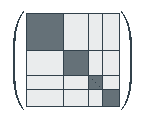
\includegraphics[height=0.8\linewidth]{../repos/hbp-paper/doc/aistats_talk/logo/hbp_logo}
    \href{https://github.com/f-dangel/hbp}{\texttt{github.com/f-dangel/hbp}}
  \end{center}} %
presents Hessian backpropagation (HBP), an extension of gradient backpropagation
to compute layer-wise curvature in sequential feedforward neural networks. Just
like gradient backpropagation recovers the gradient vectors in blocks that
correspond to layers, local curvature, \ie second-order partial derivatives of
the loss \wrt parameters in a layer can be evaluated by backpropagating
Hessians. Its computation is disentangled to the modular level, which allows for
an elegant and extensible implementation in analogy to gradient backpropagation.
We describe the backpropagation operations at the per-layer level, resulting in
an algorithm that computes local curvature in an automated fashion, and at the
same time as the gradient. Adaptations of the exact procedure recover positive
semi-definite block diagonal approximations (BDAs)---\eg of the GGN---and
recently proposed Kronecker-factored curvature approximations
\cite{martens2015optimizing,botev2017practical,wei2018bdapch} of the Hessian,
unifying their computation.

\begin{disclaimer}
  \Cref{chap:hbp} is based on the peer-reviewed conference
  paper with the following co-author contributions:

  \fullcite{dangel2020modular} \cite{dangel2020modular}

  \vspace{-1.75ex}

  \begin{center}
    \begin{tabular}[!h]{lrrrr}
      & \textbf{Ideas} & \textbf{Experiments} & \textbf{Analysis} & \textbf{Writing}
      \\
      \textbf{F.\,Dangel} & 70\,\% & 80\,\% & 70\,\% & 65\,\%
      \\
      S.\,Harmeling & 10\,\%& 10\,\% & 10\,\% & 10\,\%
      \\
      P.\,Hennig & 20\,\% & 10\,\% & 20\,\% & 25\,\%
    \end{tabular}
  \end{center}
\end{disclaimer}

\Cref{chap:backpack} \marginnote{%
  \Cref{chap:backpack}:
  \backpack: an efficient framework built on top of \PyTorch that extends the
  backpropagation algorithm.
  \begin{center}
    \vspace{-2ex} 
\includegraphics[height =
    0.8\linewidth]{../repos/backpack-paper/tex/logo/backpack_logo_github}
    \href{https://github.com/f-dangel/backpack}{\texttt{github.com/f-dangel/backpack}}
  \end{center}} %
further generalizes this idea and presents \backpack, an efficient framework
that extends the gradient backpropagation of \pytorch. The library provides
access to higher-order statistical information about the gradient distribution,
like individual gradients or an estimate of their variance, and structured
curvature information, like the Hessian/\ggn diagonal and block-diagonal
Kronecker-factored curvature approximations. This is achieved with slightly more
flexible implementations of AD functionality and by backpropagating additional
information through the graph. Importantly, most quantities add small overhead
to the gradient, making their exploration for research more attractive.

\begin{disclaimer}
  \Cref{chap:backpack} is based on the peer-reviewed
  conference publication with the following co-author contributions:

  \fullcite{dangel2020backpack} \cite{dangel2020backpack}

  \vspace{-1.75ex}

  \begin{center}
    \begin{tabular}[!h]{lrrrr}
      & \textbf{Ideas} & \textbf{Experiments} & \textbf{Analysis} & \textbf{Writing}
      \\
      \textbf{F.\,Dangel} & 33\,\% & 55\,\% & 45\,\% & 35\,\%
      \\
      F.\,Kunstner & 33\,\%& 45\,\% & 45\,\% & 45\,\%
      \\
      P.\,Hennig & 33\,\% & 0\,\% & 10\,\% & 20\,\%
    \end{tabular}
  \end{center}
\end{disclaimer}

\Cref{chap:cockpit}\marginnote{%
  \Cref{chap:cockpit}: \cockpit: a debugging tool
  for the training of deep neural networks.
  \begin{center}
    \vspace{-5ex} 
\includegraphics[height =
    0.8\linewidth]{../repos/cockpit/docs/source/_static/LogoSquare}
    \href{https://github.com/f-dangel/cockpit}{\texttt{github.com/f-dangel/cockpit}}
  \end{center}} %
introduces \cockpit, a live-monitoring debugging tool that consists of various
instruments which leverage higher-order information, efficiently provided by
\backpack. By providing a deeper look into the inner workings of neural networks
through the lens of this information, \cockpit can help identify bugs in the ML
pipeline, while keeping the computational overhead acceptable. This demonstrates
the utility of higher-order information to assist deep learning practitioners
and researchers to better understand their problems and conduct research.

\begin{disclaimer}
  \Cref{chap:cockpit} is based on the peer-reviewed
  conference paper with the following co-author contributions:

  \fullcite{schneider2021cockpit} \cite{schneider2021cockpit}

  \vspace{-1.75ex}

  \begin{center}
    \begin{tabular}[!h]{lrrrr}
      & \textbf{Ideas} & \textbf{Experiments} & \textbf{Analysis} & \textbf{Writing}
      \\
      F.\,Schneider & 45\,\%& 40\,\% & 40\,\% & 45\,\%
      \\
      \textbf{F.\,Dangel} & 40\,\% & 50\,\% & 40\,\% & 40\,\%
      \\
      P.\,Hennig & 15\,\% & 10\,\% & 20\,\% & 15\,\%
    \end{tabular}
  \end{center}
\end{disclaimer}

\Cref{chap:vivit} \marginnote{%
  \Cref{chap:vivit}: \vivit: efficient computation with the \ggn's low-rank
  structure.
  \begin{center}
    \vspace{-4ex} 
\includegraphics[height =
    0.8\linewidth]{../repos/vivit/docs/rtd/assets/vivit_logo}
    \href{https://github.com/f-dangel/vivit}{\texttt{github.com/f-dangel/vivit}}
  \end{center}}%
presents \vivit, a method that leverages the low-rank structure in the \ggn to
efficiently extract eigenvalues, eigenvectors, per-sample first- and
second-order directional derivatives, and Newton steps. In contrast to other
popular curvature approximations, \vivit is capable of tracking off-diagonal
curvature blocks, offers principled approximations to trade off cost and
accuracy, and allows studying noise in the curvature. Under the hood, \vivit's
quantities are efficiently computed during backpropagation, building on
\backpack's advanced AD functionality. This demonstrates how such functionality
enables investigations of unexplored structure in higher-order information which
may be used to develop novel algorithms and better understand challenges to make
them work in practice, \eg noise.

\begin{disclaimer}
  \Cref{chap:vivit} is based on the peer-reviewed journal paper with the
  following co-author contributions:

  \fullcite{dangel2022vivit} \cite{dangel2022vivit}

  \vspace{-1.75ex}

  \begin{center}
    \begin{tabular}[!h]{lrrrr}
      & \textbf{Ideas} & \textbf{Experiments} & \textbf{Analysis} & \textbf{Writing}
      \\
      \textbf{F.\,Dangel} & 50\,\% & 40\,\% & 40\,\% & 40\,\%
      \\
      L.\,Tatzel & 35\,\%& 50\,\% & 40\,\% & 45\,\%
      \\
      P.\,Hennig & 15\,\% & 10\,\% & 20\,\% & 15\,\%
    \end{tabular}
  \end{center}
\end{disclaimer}

\Cref{part:conclusion} summarizes the findings of this manuscript \wrt the
inital questions from \Cpageref{enum:background::Questions}, as well as their
impact and relation to the latest developments in the field. Finally, the
manuscript identifies future research directions for the presented extended AD
eco-system around \pytorch, and more broadly for the development of future ML
libraries.

%%% Local Variables:
%%% mode: latex
%%% TeX-master: "../thesis"
%%% End:


% ---------------------------------
% BACKGROUND
% ---------------------------------

\pagelayout{wide} % disable margins
\part{Background \& Motivation}\label{part:background}
\pagelayout{margin} % restore margins

\setchapterpreamble[u]{\margintoc}
\chapter{Deep Learning Components}\label{chap:background::Paradigms}
Broadly speaking, ML seeks to find a well-performing algorithm for a given task
from ``experience''. This thesis considers supervised deep learning, where
``experience'' is given through annotated examples in form of a dataset. A datum
$(\vx, \vy)$ consists of \emph{input features} $\vx$ and \emph{targets}, or
\emph{labels}, $\vy$. The algorithm, or \emph{model}, is a deep neural network
(\Cref{sec:background::DeepNeuralNetworks}) that tries to predict $\vy$ from
$\vx$ and is selected by minimizing a performance criterion on the available
data (the empirical risk, \Cref{sec:background::SupervisedLearning}) using
optimization methods which rely on automatically computed derivatives
(\Cref{sec:background::GradientBackpropagation}). This chapter reviews these
components, highlighting their structure \wrt implementation in ML libraries.
For a broader introduction to deep learning, see \eg \cite{goodfellow2016deep}.

\section{Empirical Risk Minimization}\label{sec:background::SupervisedLearning}
``Learning'' is connected to optimization by the risk minimization paradigm. The
idea is to define a performance metric that assesses the quality of the model's
prediction. Then, learning happens by maximizing that performance metric.
Conversely, one can specify a metric for the prediction's error
(also referred to as \emph{risk}), and minimize the latter.


For example, an intuitive way to assess performance for a classification task is
\emph{accuracy}, the ratio of correct and total predictions (the error would be
the ratio of incorrect and total predictions). However, such direct performance
measures are hard to optimize with derivative-based methods\sidenote{\eg the
  accuracy on one datum is either 0 or 1, and hence its derivative vanishes
  everywhere it is defined.} and must be substituted by a surrogate function
that approximates the original performance measure, but is easier to optimize.
In the deep learning terminology, these surrogates are commonly referred to as
\emph{loss functions}. This section expands on risk minimization, its
characteristic properties in deep learning, and its probabilistic
interpretation.

\subsection{Notation \& Mathematical
  Details}\label{sec:background::empiricalRiskMinimization}

\subsubsection{Risk \& Empirical Risk}

Consider supervised learning with the goal to learn the functional relation
between inputs $\vx \in \sX$ and targets $\vy \in \sY$
(\Cref{fig:background::ModelLossFunctionSplit}). The mapping is described by a
model $f_{\vtheta}: \sX \to \sF$ with adjustable parameters $\vtheta \in
\sTheta$ that produces predictions $\vf := f_{\vtheta}(\vx) \in \sF$ for an
input $\vx$. A prediction's error is assessed through a convex loss function
$\ell: \sF \times \sY \to \sR$.

\begin{figure}[tb]
  \centering \tikzexternalenable
  \resizebox{!}{3.5cm}{% Model-loss function split with data flow
\input{figures/background/model_loss_split_command}

\begin{tikzpicture}
  \drawModelLossSplit{$\vx$}{$\vf$}{$\vy$}{$\ell(\vf, \vy)$}
\end{tikzpicture}

%%% Local Variables:
%%% mode: latex
%%% TeX-master: "../../thesis"
%%% End:
}
  \tikzexternaldisable
  \caption{\textbf{Components of supervised learning:} The goal is to infer
    parameters $\vtheta$ of a model $f_{\vtheta}$, that relates inputs $\vx$ to
    predictions $\vf$, by minimizing a loss function $\ell$ between the
    prediction $\vf$ and label $\vy$.}
  \label{fig:background::ModelLossFunctionSplit}
\end{figure}

\emph{Regression} (\Cref{ex:background::Regression}) and \emph{classification}
(\Cref{ex:background::Classification}) are two common tasks that will be used
frequently in later chapters. The remainder of this text sets $\sX = \sR^{M}$
and $\sF = \sR^{C}$, with input and prediction space dimensions $M, C$,
respectively ($C$ corresponds to the number of classes for classification).
Because the discussion focuses on neural networks as model, it sets $\sTheta =
\sR^{D}$ in what follows.

\begin{figure}[!b]
  \begin{example}[\textbf{Least squares regression \& square
      loss}]\label{ex:background::Regression}
    Regression associates features in $\sX = \sR^M$ with targets in $\sY =
    \sR^C$. A prediction in $\sF = \sR^{C}$ compares to its ground truth via the
    mean squared error\sidenote{%
      There exist different conventions for the normalization factor. This text
      adapts the implementation of
      \inlinecode{\href{https://pytorch.org/docs/1.11/generated/torch.nn.MSELoss.html\#torch.nn.MSELoss}{MSELoss}}
      (with \inlinecode{reduction="mean"} mode) in \pytorch for consistency with
      the code presented in later chapters. Normalizing by $\nicefrac{1}{C}$ is
      also close to what the name, mean squared error, suggests.}
    \begin{align}\label{eq:background::squareLoss}
      \ell(\vf, \vy)
      =
      \frac{1}{C} \sum_{c=1}^C (\evy_c - \evf_c)^2
      =
      \frac{1}{C} \lVert \vy - \vf  \rVert_{2}^{2}
    \end{align}
  \end{example}
  \begin{example}[\textbf{$C$-class classification \& softmax cross-entropy
      loss}]\label{ex:background::Classification}
    Classification assigns features in $\sX = \sR^{M}$ to classes in $\sY =
    \left\{ 1, \dots, C \right\}$ using a model to $\sF = \sR^C$. The softmax
    cross-entropy loss\sidenote{%
      Sometimes, the softmax is considered part of the model rather than the
      loss function. This text assigns it to the loss function, in line with the
      \pytorch implementation of
      \inlinecode{\href{https://pytorch.org/docs/1.11/generated/torch.nn.CrossEntropyLoss.html\#torch.nn.CrossEntropyLoss}{CrossEntropyLoss}},
      that combines softmax and cross-entropy, which is numerically more
      stable~\cite[][Chapter 4]{goodfellow2016deep}.}%
    maps the model's prediction to a probability distribution over classes, then
    uses cross-entropy to compare it with the ground truth,
    \begin{align}
      \label{eq:background::softmaxCrossEntropyLoss}
      \ell(\vf, y) = - \log([p(\vf)]_{y})
      =
      - {\log p(\vf)}^\top \onehot(y)
    \end{align}
    where $p(\vf) = \softmax(\vf)$ and $[\onehot(y)]_{c} = \delta_{c,y}$.
  \end{example}
\end{figure}

% \paragraph{Risk minimization:}
Assume that the population of input-target pairs,
\ie the \emph{data-generating process}, follows a distribution $\pdata(\vx,
\vy)$. A model's expected risk under this distribution is defined as
\begin{subequations}
  \begin{align}
    \label{eq:background::expectedRisk}
    \begin{split}
      \gL_{\pdata}(\vtheta)
      &:=
        \E_{\pdata(\vx, \vy)}
        \left[
        \ell(f_{\vtheta}(\vx), \vy)
        \right]
      \\
      &=
        \iint_{\sX,\sY}
        \ell(f_{\vtheta}(\vx), \vy)
        \pdata(\vx, \vy)
        \,\diff\vx\,\diff\vy\,.
    \end{split}
  \end{align}
  The incentive for a model to perform well is to achieve a small expected risk.
  Therefore, training a model is minimizing \Cref{eq:background::expectedRisk},
  \begin{equation}
    \label{eq:background::minimizeExpectedRisk}
    \minimize_{\vtheta} \gL_{\pdata}(\vtheta)\,.
  \end{equation}
\end{subequations}

% \paragraph{Empirical approximation:}
But in practice, \Cref{eq:background::minimizeExpectedRisk} is inaccessible
because the data-generating process $\pdata(\vx, \vy)$ is unknown. Instead, the
problem is approximated through an \iid dataset $\sD = \{ (\vx_n, \vy_n) \in \sX
\times \sY \}_n$ of labeled data collected from $\pdata(\vx,\vy)$. $\pdata(\vx,
\vy)$ is approximated by the empirical distribution
\begin{subequations}\label{eq:background::supervisedLearning}
  \begin{equation}
    \label{eq:background::empiricalDistribution}
    p_{\sD}(\vx, \vy)
    =
    \frac{1}{|\sD|}
    \sum_{(\vx_{n}, \vy_{n}) \in \sD}
    \delta(\vx - \vx_{n}) \delta(\vy - \vy_{n})
  \end{equation}
  implied by $\sD$. The model's empirical risk on $\sD$ follows from
  substituting $\pdata$ with $p_{\sD}$ in \Cref{eq:background::expectedRisk},
  which yields
  \begin{equation}
    \label{eq:background::empiricalRisk}
    \gL_{\sD}(\vtheta)
    :=
    \gL_{p_{\sD}}(\vtheta)
    =
    \frac{1}{|\sD|}
    \sum_{(\vx_{n}, \vy_{n}) \in \sD}
    \ell(f_{\vtheta}(\vx_{n}), \vy_{n})\,.
  \end{equation}
  In practice, learning happens by minimizing an empirical risk,
  \begin{equation}
    \label{eq:background::empiricalRiskMinimization}
    \minimize_{\vtheta} \gL_{\sD}(\vtheta)\,.
  \end{equation}
\end{subequations}

\subsubsection{Challenges for Optimization}

Training a model relies on optimization algorithms which are initialized at some
$\vtheta_{0}\in \sTheta$ and seek to iteratively improve the solution to
\Cref{eq:background::empiricalRiskMinimization}. At an iteration $t$, the
optimizer is given access to information about the objective at $\vtheta_t$,
like derivatives (\Cref{sec:background::GradientBackpropagation}), to deduct a
step $\vtheta_{t+1} \leftarrow \vtheta_t$, potentially using additional
information from past observations. In general, the more local information is
available, the more powerful a single update step can be. But richer information
is often more costly to compute. The large-scale nature of deep learning poses
challenges on the accessible information:
\begin{itemize}

\item \textbf{Big data:} deep learning datasets are often large because more
  data gives better approximations of the true distribution $\pdata$ via
  $p_{\sD}$, and thus better task performance. The simultaneous computation of
  all per-datum losses for $\gL_{\sD}(\vtheta)$ does not fit into memory (for
  many contemporary tasks, it is even infeasible to hold $\sD$ in
  memory\sidenote{%
    \Eg \imagenet~\cite{deng2009imagenet} consists of 1,281,167 training images.
    The Kaggle download requires roughly 166\,GB of memory.%
  }). Still, to obtain $\gL_{\sD}$, one could sequentially compute and reduce
  its summands on data chunks of manageable size. In practice, it is more common
  though to approximate $\gL_{\sD}$ on a randomly drawn small subset, a
  mini-batch, $\sB \subseteq \sD$ with $|\sB| \ll |\sD|$. While this avoids a
  computationally expensive full sweep over the data, subsampling introduces
  \emph{noise} in the loss (\Cref{sec:background::MiniBatching}). This noise is
  inherited by the computed information supplied to the optimizer. Algorithms
  must therefore take into account the stochastic nature of their observations.

\item \textbf{Very large models:} the parameter space dimension $D$ of DNNs
  usually exceeds the (already large) amount of data $|\sD|$, \ie $D \gg |\sD|$.
  It affects the complexity to store and compute information, such as
  derivatives of the loss \wrt $\vtheta$, and makes it more challenging to
  efficiently work with higher-order information\sidenote{%
    For example, interesting quantities for an optimizer are the loss
    landscape's local slope (gradient) and curvature (Hessian,
    \Cref{def:background::Hessian}). While the gradient is cheap to compute and
    store ($D$ elements), holding the $D\times D$ Hessian in memory is
    infeasible.%
  }. Therefore, working with higher-order information relies on implicit schemes
  (\eg matrix-free Hessian-vector products~\cite{pearlmutter1994fast}) or
  light-weight structured approximations (\eg through Kronecker
  products~\cite{martens2015optimizing}). Such approaches are usually technical
  and challenging to implement. They also add significant computational work
  that must be compensated for by an improved update step quality in optimizers.
\end{itemize}
In addition to these computational aspects, there exist other challenges:
\begin{itemize}
\item \textbf{Non-convexity:} although the loss function $\ell$ is convex \wrt
  the model's output $\vf$, convexity does not carry through to the model's
  parameters\sidenote[][-2.5\baselineskip]{Convexity of $\ell$ in $\vf$ is still
    useful to construct PSD approximations to the Hessian, see
    \Cref{sec:background::ggn}.}. This is because DNNs $f_{\vtheta}$ are highly
  non-linear, and therefore generally non-convex, in $\vtheta$. Local minima of
  convex functions are global minima, meaning that local improvement gets us
  closer to a global solution. But non-convex problems like
  \Cref{eq:background::empiricalRiskMinimization} have multiple local minima
  that need not be global. Through local improvements, an optimizer can arrive
  at one of these local minima, but with no path of improvement to a global
  solution. This depends on various aspects, such as the update rule,
  hyperparameters, initialization, \etc.

\item \textbf{Generalization:} learning is not pure optimization. While
  minimizing the empirical risk \Cref{eq:background::empiricalRiskMinimization}
  improves the model's performance on the collected data, the actual goal is to
  obtain good performance on new unseen data, \ie generalize well. To achieve
  generalization, it is crucial to prevent optimization to overfit specifics in
  the data.
  % train-test split
  It is common practice to split the data into three disjoint sets $\Dtrain$,
  $\Dvalid$, and $\Dtest$. The train set's empirical risk
  $\gL_{\Dtrain}(\vtheta)$ is minimized, and the validation loss
  $\gL_{\Dvalid}(\vtheta)$ serves to identify hyperparameters that lead to
  generalization on $\Dvalid$. The held-out examples in the test set $\Dtest$
  are used to assess generalization to new data.
  % data augmentation
  Another way to improve generalization is to use more data during training.
  Data augmentation~\cite{shorten2019survey} allows for cheap generation of new
  examples without collecting new data.
  % regularization
  Sometimes, it may be desirable to penalize model properties by adding a
  regularization term to the objective in
  \Cref{eq:background::empiricalRiskMinimization}.
\end{itemize}

\subsection{Batching \& Noise}\label{sec:background::MiniBatching}

Due to the large-scale nature of $\sD$ and $f_{\vtheta}$ in the empirical risk,
\Cref{eq:background::empiricalRisk} is usually stochastically approximated
through a mini-batch $\sB \subseteq \sD$, and assessed through a mini-batch loss
\begin{equation}
  \label{eq:background::miniBatchRisk}
  \gL_{\sB}(\vtheta)
  =
  \frac{1}{|\sB|}
  \sum_{(\vx_n, \vy_n) \in \sB}
  \ell(f_{\vtheta}(\vx_n), \vy_n)\,.
\end{equation}
In the following, per-sample predictions and losses will often be abbreviated as
$\vf_n := f_{\vtheta}(\vx_n)$ and $\ell_n := \ell(f_{\vtheta}(\vx_n), \vy_n)$.

\subsubsection{Batched Computations}

Evaluation of the mini-batch loss in \Cref{eq:background::miniBatchRisk} can be
parallelized (\Cref{subfig:background::BatchedComputation1}). All mini-batch
features $\{ \vx_n \}$ are mapped to predictions $\{ \vf_n \}$ by the \emph{same
  instructions $f_{\vtheta}$}, and compared in parallel with the labels $\{
\vy_n \}$, resulting in the per-sample losses $\{ \ell_n\}$. Hardware
accelerators can use this structure to achieve significant speed-up of
evaluating the loss, or its derivatives
(\Cref{sec:background::GradientBackpropagation}).

\begin{figure*}[t]
  \centering
  \begin{subfigure}[t]{0.495\linewidth}
    \centering
    \caption{Same instructions, multiple data}
    \label{subfig:background::BatchedComputation1}
    \tikzexternalenable
    \resizebox{!}{3.5cm}{\input{figures/background/model_loss_split_command}

\begin{tikzpicture}
  \foreach \x in {1,2,3} {
    \pgfmathsetmacro{\xshiftcm}{-0.2 * (\x - 1)}
    \pgfmathsetmacro{\yshiftcm}{-0.6 * (\x - 1)}
    \begin{scope}[xshift = \xshiftcm cm, yshift = \yshiftcm cm, opacity = 0.95]
      \drawModelLossSplit{$\vx_{\x}$}{$\vf_{\x}$}{$\vy_{\x}$}{$\ell_{\x}$}
    \end{scope}
   }
\end{tikzpicture}

%%% Local Variables:
%%% mode: latex
%%% TeX-master: "../../thesis"
%%% End:
}
    \tikzexternaldisable
  \end{subfigure}
  \hfill
  \begin{subfigure}[t]{0.495\linewidth}
    \centering
    \caption{Batched operations}
    \label{subfig:background::BatchedComputation2}
    \tikzexternalenable
    \resizebox{!}{3.5cm}{\input{figures/background/model_loss_split_command}

\begin{tikzpicture}
  \drawModelLossSplit{%
    $\left\{\vx_n\right\}$}{%
    $\left\{\vf_n\right\}$}{%
    $\left\{\vy_n\right\}$}{%
    $\left\{\ell_n\right\}$}
\end{tikzpicture}

%%% Local Variables:
%%% mode: latex
%%% TeX-master: "../../thesis"
%%% End:
}
    \tikzexternaldisable
  \end{subfigure}
  \caption{\textbf{Different visualizations of empirical risk computation
      graphs.} \subfigref{subfig:background::BatchedComputation1}, The empirical
    risk is a weighted sum of per-sample losses that are computed independently
    and with the same instructions, allowing for efficient parallelization.
    \subfigref{subfig:background::BatchedComputation2} Many ML libraries
    natively support batched operations for efficiency. In code, this batching
    is often assumed, but not explicitly expressed. The $\vmap$ concept allows
    to make batching explicit: $f_{\vtheta}$ and $\ell$ in
    \subfigref{subfig:background::BatchedComputation2} correspond to vectorized
    versions $\vmap(f)$ and $\vmap(\ell)$ from
    \subfigref{subfig:background::BatchedComputation1}.}
  \label{fig:background::BatchedComputation}
\end{figure*}

This single-instruction-multiple-data structure of the loss is often baked into
ML libraries. Many of their operations natively support batched behavior, \ie
accept stacked inputs and assume one, usually the first, axis to correspond to a
batch axis. The operation is then applied to all slices along the batch axis
(\Cref{subfig:background::BatchedComputation2}).

The concept of \inlinecode{map} in functional
programming~\cite{hughes1989functional} formalizes applying a function to a
collection of inputs, which can be seen as a function transformation. Batched
operations can be understood as transformations of the original operation.
Recently developed ML libraries~\cite{bradbury2018jax,he2021functorch} make
batching explicit by providing a $\inlinecode{vmap}$ interface to automatically
vectorize, \ie parallelize, the application of \inlinecode{map}.

\begin{definition}[\textbf{vmap}]\label{def:background::vmap} Let $f: \sX \to
  \sY, x \mapsto f(x)$ denote a function. The vectorized \inlinecode{map},
  $\vmap(f)$, of $f$ \wrt its argument $x$ is a function that accepts a
  collection of inputs and maps each item by $f$, resulting in a collection of
  outputs,
  \begin{align*}
    \vmap:\quad (\sX \to \sY)
    \to (\sX^{N} \to \sY^{N})
    \quad \forall\,N \in \sN
    \shortintertext{such that}
    \vmap(f)(\{ x_1, x_2, \dots, x_N\})
    =
    \{f(x_1), f(x_2), \dots, f(x_N)\}\,.
  \end{align*}
  Collections are often abbreviated as $\{x_n\} := \{ x_1, x_2, \dots, x_N\}$
  and $\{f(x_n)\} := \{f(x_1), f(x_2), \dots, f(x_N)\}$. Multi-variate functions
  can be mapped \wrt to a subset of arguments.
\end{definition}

Making batching explicit with \inlinecode{map}, the mini-batch loss computation
uses a vectorized model $\vmap(f_{\vtheta})$ \wrt the input features
$\vx$, such that
\begin{subequations}
  \begin{align}
    \vmap(f_{\vtheta})(\{ \vx_n\}) &= \{ \vf_{n}(\vtheta) \}\,.
  \end{align}
  Per-sample losses, which are reduced into the mini-batch loss, are
  \begin{align}
    \{ \ell_n(\vtheta) \}
    &=
      \vmap(\ell)(\{ \vf_{n}(\vtheta) \}, \{ \vy_n \})\,.
  \end{align}
\end{subequations}
Numerically, collections of vectors like $\{\vx_n\}$ \etc are represented as
matrices, and more generally, collections of $r$-dimensional arrays are stacked
into a $(r+1)$-dimensional arrays with an additional batch axis (\eg, $\{ \vx_n
\}$ is a $|\sB| \times M$ matrix). These arrays can then be efficiently
processed in hardware accelerators.

\subsubsection{Noise}

While
%
\marginnote[*-12]{
  \begin{center}
    \tikzexternalenable
    \resizebox{\linewidth}{!}{\input{figures/background/model_loss_split_command_hotfix}

\begin{tikzpicture}
  \pgfmathsetseed{42}
  \foreach \x in {1,2,3,4,5} {
    \pgfmathsetmacro{\xshiftcm}{-0.2 * (\x - 1)}
    \pgfmathsetmacro{\yshiftcm}{-0.6 * (\x - 1)}
    \pgfmathrandominteger{\opacitySwitch}{0}{10}
    \ifthenelse{\opacitySwitch > 6}{%
      \pgfmathsetmacro{\opacity}{0.15}}{%
      \pgfmathsetmacro{\opacity}{0.95}}
    % \node [opacity=\opacity] at (\x, 0) {\opacitySwitch};
    \begin{scope}[xshift = \xshiftcm cm, yshift = \yshiftcm cm, opacity = \opacity]
      \drawModelLossSplit{$\vx_{\x}$}{$\vf_{\x}$}{$\vy_{\x}$}{$\ell_{\x}$}
    \end{scope}
  }
\end{tikzpicture}

%%% Local Variables:
%%% mode: latex
%%% TeX-master: "../../thesis"
%%% End:
}
    \tikzexternaldisable
  \end{center}
  \captionof{figure}{\textbf{Illustration of stochastic sub-sampling:} The
    computation graph of the empirical risk (with five data in this example) is
    only evaluated on a subset of data (two in this example) to save
    computations. While this preserves parallelization, the transparent parts
    are not evaluated, which introduces noise.}\label{fig:background::MiniBatch}
}%
the sum structure in the loss \Cref{eq:background::empiricalRisk} can be
efficiently parallelized, it can also be used for stochastic approximation via
sub-sampling (\Cref{fig:background::MiniBatch}). The mini-batch loss $\gL_\sB$
in \Cref{eq:background::miniBatchRisk} is an estimator of the empirical risk
$\gL_\sD$ implied by the stochastic sampling procedure of $\sB$. Increasing the
batch size makes this estimator more precise but more costly to compute.


% Batch size = 1
To see this cost-accuracy trade-off, consider the loss of a single datum
$\ell_n$ where $n$ is uniformly drawn from $\{1, \dots, |\sD|\}$.
Then, $\ell_n$ is a random variable, implied by the sampling distribution $n \sim
p(n) = \gU(\{1, \dots, |\sD|\})$, and an unbiased estimator of the empirical risk,
\begin{subequations}
  \begin{align}\label{eq:background::unbiasedEstimator}
    \E_{p(n)}[\ell_n(\vtheta)]
    &=
      \sum_{n=1}^{|\sD|} p(n) \ell_n(\vtheta)
      =
      \gL_{\sD}(\vtheta)\,,
  \end{align}
  with variance
  \begin{align}
    \label{eq:background::unbiasedEstimatorVariance}
    \begin{split}
      \sigma^{2}
      :=
      \Var_{p(n)}[\ell_n(\vtheta)]
      &=
        \E_{p(n)}\left[(\ell_n(\vtheta) - \gL_{\sD}(\vtheta))^2\right]
      \\
      &=
        \E_{p(n)}\left[\ell_n(\vtheta)^2\right]
        -
        \gL_{\sD}(\vtheta)^2\,.
    \end{split}
  \end{align}
\end{subequations}
% Batch size B
Next, consider a batch with $\sB|$ randomly drawn samples $\vn = (n_1, \dots,
n_{|\sB|})$ from a joint distribution $p(\vn)$, \ie the mean of $\ell_{n_1},
\dots, \ell_{n_{|\sB|}}$,
\begin{subequations}
  \begin{align}
    \gL_{\vn}(\vtheta)
    &=
      \frac{1}{|\sB|}
      \sum_{i=1}^{|\sB|} \ell_{n_i}(\vtheta)\,.
  \end{align}
  If samples are drawn uniformly \iid ($p(\vn) = \prod_{i=1}^{|\sB|} p(n_i)$
  with $p(n_i) = \gU(\{1, \dots, |\sD|\})$), this estimator is also unbiased,
  \begin{align}
    \label{eq:background::unbiasedBatchEstimator}
    \E_{p(\vn)}[\gL_\vn(\vtheta)]
    =
    \frac{1}{|\sB|}
    \sum_{i=1}^{|\sB|} \E_{p(n_i)}[\ell_{n_i}(\vtheta)]
    =
    \gL_{\sD}(\vtheta)\,,
  \end{align}
  but has smaller variance than the single-sample estimator:
  \begin{align}
    \label{eq:background::varianceBatchEstimator}
    \Var_{p(\vn)}[\gL_{\vn}(\vtheta)]
    =
    \E_{p(\vn)}[\gL_\vn(\vtheta)^2] - \gL_{\sD}(\vtheta)^2
    =
    \frac{\sigma^{2}}{|\sB|}\,.
  \end{align}
  Using more samples, \ie a larger $|\sB|$, decreases the variance, and thereby
  reduces noise in the mini-batch loss.
\end{subequations}
The central limit theorem~\cite{fischer2010history} connects the mini-batch
estimator to a normal distribution. As the mini-batch size $|\sB|$ approaches
infinity, $\gL_{\vn}$ converges to a normal distribution with mean and variance
from
\Cref{eq:background::unbiasedBatchEstimator,eq:background::varianceBatchEstimator}
\begin{align}\label{eq:background::CentralLimitTheorem}
  \lim_{|\sB| \to \infty}:
  \quad
  \gL_{\vn}
  \sim
  \gN(
  \giventhat{
  \gL_{\vn}
  }
  {
  \gL_{\sD},
  \nicefrac{\sigma^{2}}{|\sB|}
  }
  )\,.
\end{align}
While applications rely on finite batch sizes, it is sometimes useful to assume
that this Gaussian distribution holds approximately.

Noise in the mini-batch loss propagates to other quantities, like the mini-batch
gradient $\grad{\vtheta}\gL_{\sB}(\vtheta)$, that are used for applications like
training. Therefore, it represents a fundamental challenge for deep learning
methods. It can be assessed through higher-order statistical moments such as the
variance (the centered second moment, see
\Cref{sec:background::gradientCovariance,cockpit::app:instruments} for
examples). Motivated by the central limit theorem
\Cref{eq:background::CentralLimitTheorem}---if the Gaussian approximation holds
sufficiently well---only second-order statistical moments are required.

Like higher-order derivatives of multi-variate functions, higher-order
statistical moments of multi-variate random variables such as the mini-batch
gradient $\grad{\vtheta}\gL_{\sB}(\vtheta) \in \sR^D$ (first moment) scale
exponentially with dimension $D$ (\eg the $D \times D$ gradient covariance
matrix, \Cref{sec:background::gradientCovariance}). Therefore, they are
challenging to work with using naive approaches.

\subsection{Probabilistic
  Interpretation}\label{sec:background::ProbabilisticInterpretation}

Risk-based supervised learning is often connected to learning the unknown true
distribution $\pdata(\vx, \vy)$ through a model distribution $p_{\vtheta}(\vx,
\vy)$ and data $\sD$, using estimation techniques to finding a good set of
parameters that minimizes a measure of dissimilarity between $\pdata$ and
$p_{\vtheta}$. The following section links the loss function $\ell$ and the
model $f_{\vtheta}$ to probabilistic objects. This will be helpful to identify
additional structure in the risk minimization problem and use it for structural
approximation of higher-order information (\eg the Fisher information matrix,
\Cref{sec:background::naturalGradientDescent}), and to motivate probabilistic
applications (\eg Laplace approximations,
\Cref{sec:background::LaplaceApproximation}).

\subsubsection{Connections to Maximum Likelihood Estimation (MLE)}
The KL-divergence between the true and the model distribution,
\begin{subequations}
  \begin{align}
    \label{eq:background::KLDivergence}
    \begin{split}
      &\KLdiv{\pdata(\vx, \vy)}{p_{\vtheta}(\vx, \vy)}
      \\
      &\quad =
        \E_{\pdata(\vx, \vy)}
        \left[
        \log\pdata(\vx, \vy)
        -
        \log p_{\vtheta}(\vx, \vy)
        \right]\,,
    \end{split}
  \end{align}
  can be used to measure their dissimilarity. Minimizing the above expression
  over $\vtheta$, and dropping parameter-independent terms leads to
  \begin{align}
    \label{eq:background::minimizeNegativeLogProbability}
    \begin{split}
      &\minimize_{\vtheta}
        \KLdiv{\pdata(\vx, \vy)}{p_{\vtheta}(\vx, \vy)}
      \\
      \Leftrightarrow
      &\minimize_{\vtheta}
        \E_{\pdata(\vx, \vy)}
        \left[
        - \log p_{\vtheta}(\vx, \vy)
        \right]\,.
    \end{split}
  \end{align}
  $\pdata(\vx, \vy)$ is inaccessible and therefore empirically approximated
  through data $\sD = \{ (\vx_n, \vy_n) \}_n$. Under the \iid assumption in the
  data, $\pdata$ is replaced with the empirical distribution $p_{\sD}$ from
  \Cref{eq:background::empiricalDistribution} and yields the accessible
  optimization task
  \begin{align}
    \label{eq:background::minimizeEmpiricalNegativeLogProbability}
    \minimize_{\vtheta}
    \frac{1}{|\sD|}
    \sum_{(\vx_{n}, \vy_{n}) \in \sD} - \log p_{\vtheta}(\vx_n, \vy_n)
  \end{align}
  This expression resembles the empirical risk minimization
  \Cref{eq:background::empiricalRiskMinimization} with a specific loss function
  $\ell$ that produces the negative log-probability of a datum $(\vx_n,\vy_n)$.
\end{subequations}

\begin{subequations}
  Supervised learning only processes features $\vx$ to predict labels $\vy$. The
  probabilistic model $p_{\vtheta}(\vx, \vy)$ thus has a more special form, in
  that it only parameterizes the likelihood $\giventhat{\vy}{\vx}$,
  \begin{align}
    \label{eq:background::modelOnlyLikelihood}
    p_{\vtheta}(\vx, \vy) = p_{\vtheta}(\giventhat{\vy}{\vx}) p(\vx)\,.
  \end{align}
  Since only the likelihood contains parameters,
  \Cref{eq:background::minimizeNegativeLogProbability} simplifies to minimizing
  the expected negative log-likelihood
  \begin{align*}
    &\minimize_{\vtheta}
      \E_{\pdata(\vx, \vy)}
      \left[
      - \log p_{\vtheta}(\giventhat{\vy}{\vx}) - \log p(\vx)
      \right]
    \\
    \Leftrightarrow
    &\minimize_{\vtheta}
      \E_{\pdata(\vx, \vy)}
      \left[
      - \log p_{\vtheta}(\giventhat{\vy}{\vx})
      \right]
  \end{align*}
  and with empirical approximation through \iid data as \Cref{eq:background::minimizeEmpiricalNegativeLogProbability},
  \begin{align}
    \label{eq:background::mnimizeEmpiricalNegativeLogLikelihood}
    \minimize_{\vtheta}
    \frac{1}{|\sD|}
    \sum_{(\vx_{n}, \vy_{n}) \in \sD}
    - \log p_{\vtheta}(\giventhat{\vy_n}{\vx_n})\,.
  \end{align}
\end{subequations}
This minimization problem corresponds to MLE\sidenote{%
  \label{side:background::MLE}
  Finding the negative log-likelihood's minimum,
  \Cref{eq:background::mnimizeEmpiricalNegativeLogLikelihood}, is equivalent to
  finding the maximum of the \iid data's likelihood
  \begin{align*}
    p(\giventhat{\sD}{\vtheta})
    =
    \prod_{(\vx_n, \vy_n)\in\sD}
    p_{\vtheta}(\giventhat{\vy_n}{\vx_n})
    p(\vx_n)\,.
  \end{align*}
  The MLE satisfies
  \begin{align*}
    \vtheta_{\text{MLE}}
    &= \argmax p(\giventhat{\sD}{\vtheta})
    \\
    &= \argmax \log p(\giventhat{\sD}{\vtheta})
    \\
    &= \argmin - \log p(\giventhat{\sD}{\vtheta})\,.
  \end{align*}
  Inserting $p(\giventhat{\vtheta}{\sD})$ and dropping parameter-independent
  terms recovers the problem
  \Cref{eq:background::mnimizeEmpiricalNegativeLogLikelihood}.} with a
statistical model $p_{\vtheta}(\giventhat{\vy}{\vx})$. This is a specific form
of empirical risk minimization where the model's prediction $f_{\vtheta}(\vx)$
parameterizes a likelihood $q$ for $\giventhat{\vy}{\vf}$, and a negative
log-likelihood loss function $\ell$, \ie
\begin{subequations}
  \label{eq:background::connectionsMLEandEmpiricalRiskMinimization}
  \begin{align}
    p_{\vtheta}(\giventhat{\vy}{\vx}) &= q(\giventhat{\vy}{f_{\vtheta}(\vx)})\,,
    \\
    \ell(\vf, \vy) &= - \log q(\giventhat{\vy}{\vf})\,.
  \end{align}
\end{subequations}
Both the square loss and softmax cross-entropy loss
(\Cref{ex:background::Regression,ex:background::Classification}) have such a
probabilistic interpretation, see
\Cref{ex:background::probabilisticInterpretationMSELoss,ex:background::probabilisticInterpretationCrossEntropyLoss}.

\begin{example}[\textbf{Probabilistic interpretation of square
    loss}]\label{ex:background::probabilisticInterpretationMSELoss} The square
  loss \Cref{eq:background::squareLoss} is the negative log-likelihood of a
  Gaussian centered around the model's prediction with diagonal constant
  covariance,
  \begin{align*}
    \ell(\vf, \vy) &= -\log q(\giventhat{\vy}{\vf})
    \\
    \text{with}\quad
    q(\giventhat{\vy}{f_{\vtheta}(\vx)}) &= \gN(\giventhat{\vy}{\vmu, \mSigma})
  \end{align*}
  where%
  \sidenote[][-4\baselineskip]{Inserting mean and covariance into the negative
    log-probability yields,
    \begin{align*}
      -& \log \gN(\vy; \vmu, \mSigma)
      \\
       &=
         \nicefrac{1}{2} (\vy - \vmu)^{\top} \mSigma^{-1} (\vy - \vmu)
      \\
       &\phantom{=}
         + \nicefrac{1}{2}
         \left[
         \log\det\mSigma
         + C \log 2\pi
         \right]\,,
    \end{align*}
    \ie the square loss \Cref{eq:background::squareLoss} up to a
    $\vtheta$-independent term which does not affect optimization.}
  %
  $\vmu = f_{\vtheta}(\vx)$ and $\mSigma = \nicefrac{C}{2} \mI$.
\end{example}

\begin{example}[\textbf{Probabilistic interpretation of softmax cross-entropy
    loss}]\label{ex:background::probabilisticInterpretationCrossEntropyLoss}
  The softmax cross-entropy loss \Cref{eq:background::softmaxCrossEntropyLoss}
  is the negative log-likelihood of a multinomial distribution parameterized by
  the softmax probabilities,
  \begin{align*}
    \ell(\vf, y) &= -\log q(\giventhat{y}{\vf})
    \\
    \text{with}\quad
    q(\giventhat{y}{f_{\vtheta}(\vx)}) &= \Cat(y; \vp)
  \end{align*}
  where%
  \sidenote[][-4\baselineskip]{ With $\evp_{c}$ denoting the probability to observe class $y=c$,
    \begin{align*}
      - \log \Cat(y; \vp) = -\log \evp_{y}\,,
    \end{align*}
    which is the softmax cross-entropy loss \Cref{eq:background::softmaxCrossEntropyLoss}.}
  %
  $\vp = \softmax(f_{\vtheta}(\vx))$.
\end{example}

Following the maximum likelihood principle results in the MLE parameter
$\vtheta_{\text{MLE}}$ which satisfies
\Cref{eq:background::mnimizeEmpiricalNegativeLogLikelihood} and gives rise to
the distribution $p_{\vtheta_{\text{MLE}}}(\giventhat{\vy}{\vx}) =
q(\giventhat{\vy}{f_{\vtheta_{\text{MLE}}}(\vx)})$ as an approximation to $\pdata(\giventhat{\vy}{\vx})$.

\subsubsection{Connections to Maximum A Posteriori (MAP) Estimation}
MLE maximizes the likelihood $ p(\giventhat{\sD}{\vtheta})$. In a probabilistic
formulation with a prior $p(\vtheta)$ over the parameters and evidence $p(\sD) =
\int_{\sTheta} p(\giventhat{\sD}{\vtheta}) p(\vtheta)\,\diff \vtheta$ for the
data, one can instead consider the posterior
\begin{align}
  \label{eq:background::BayesRule}
  p(\giventhat{\vtheta}{\sD})
  =
  \frac{
  p(\giventhat{\sD}{\vtheta}) p(\vtheta)
  }{
  p(\sD)
  }\,
\end{align}
which corrects the prior with data observations. Such a posterior is useful to
form probabilistic beliefs over predictions $\vy_{\star}$ for new inputs
$\vx_{\star}$,
\begin{align}
  \label{eq:background::BayesianPrediction}
  \begin{split}
    p(\giventhat{\vy_{\star}}{\vx_{\star}, \sD})
    &=
      \int_{\sTheta} p(\giventhat{\vy_{\star}}{\vx_{\star}, \sD, \vtheta})
      p(\giventhat{\vtheta}{\vx_{\star}, \sD})\,\diff \vtheta
    \\
    &=
      \int_{\sTheta} p(\vy_{\star} | \vx_{\star}, \vtheta)
      p(\giventhat{\vtheta}{\sD})\,\diff \vtheta\,.
  \end{split}
\end{align}
However, this requires integration over the posterior, which itself is almost
always intractable and thus needs to be approximated.

The MAP principle approximates the posterior with a delta distribution around
the posterior mode, \ie the point of maximum posterior density,
\begin{align}
  \label{eq:background::MAP}
  p(\giventhat{\vtheta}{\sD})
  \approx
  \delta(\vtheta - \vtheta_{\text{MAP}})
  \quad\text{where}\quad
  \vtheta_{\text{MAP}}
  =
  \argmax_{\vtheta} p(\giventhat{\vtheta}{\sD})\,.
\end{align}
It is connected to empirical risk minimization with a regularization term that
results from the prior $p(\vtheta)$. To see this, reformulate
\Cref{eq:background::MAP} to minimize the negative log-posterior, expand Baye's
rule (\Cref{eq:background::BayesRule}) and neglect the parameter-independent
evidence term. Then, apply the same assumptions as for MLE\sidenote{%
  Mathematically, they translate into
  \begin{align*}
    \begin{split}
      &p(\giventhat{\sD}{\vtheta})
      \\
      &\quad =
        \prod_{n}
        p(\giventhat{\vx_{n}, \vy_{n}}{\vtheta})
      \\
      &\quad =
        \prod_{n}
        p(\giventhat{\vy_{n}}{\vx_{n}, \vtheta}) p(\giventhat{\vx_{n}}{\vtheta})
      \\
      &\quad =
        \prod_{n}
        p(\giventhat{\vy_{n}}{\vx_n, \vtheta}) p(\vx_{n})\,
    \end{split}
  \end{align*}
  with slightly different notation for $\vtheta$ in comparison to the MLE
  discussion, as it is now treated probabilistically. }, \ie \iid data and
$\vtheta$ only parameterizing the likelihood $\giventhat{\vy}{\vx}$. This yields
\begin{align}
  \label{eq:background::MAPRelationToEmpiricalRiskMinimization}
  \begin{split}
    \vtheta_{\text{MAP}}
    &= \argmin_{\vtheta} -\log p(\giventhat{\vtheta}{\sD})
    \\
    &= \argmin_{\vtheta} -\log p(\giventhat{\sD}{\vtheta}) - \log p(\vtheta)
    \\
    &= \argmin_{\vtheta} \sum_{(\vx_n,\vy_n) \in \sD}
      -\log p(\giventhat{\vy_n}{\vx_n, \vtheta})
      -\log p(\vtheta)
    \\
    &= \argmin_{\vtheta}
      \frac{1}{|\sD|}
      \sum_{(\vx_n,\vy_n) \in \sD}
      -\log p(\giventhat{\vy_n}{\vx_n, \vtheta})
      -\frac{\log p(\vtheta)}{|\sD|}\,.
  \end{split}
\end{align}
In analogy to \Cref{eq:background::connectionsMLEandEmpiricalRiskMinimization},
the first term is an empirical risk
(\Cref{eq:background::mnimizeEmpiricalNegativeLogLikelihood}) with negative
log-likelihood loss of a distribution $q$ for targets given model predictions,
\begin{align}\label{eq:background::connectionsMAPandEmpiricalRiskMinimization}
  p(\giventhat{\vy}{\vx,\vtheta})
  = q(\giventhat{\vy}{f_{\vtheta}(\vx)})
  \quad\text{and}\quad
  \ell(\vf, \vy)
  = - \log q(\giventhat{\vy}{\vf})\,.
\end{align}
However, this risk is extended by a regularization term from the prior,
\begin{align}\label{eq:background::MAPLoss}
  \vtheta_{\text{MAP}}
  =
  \argmin_{\vtheta}
  \gL_\sD(\vtheta) + r(\vtheta)
  \quad
  \text{where}
  \quad
  r(\vtheta) = - \frac{\log p(\vtheta)}{|\sD|}\,.
\end{align}
\Cref{eq:background::MAPRelationToEmpiricalRiskMinimization,eq:background::MAPLoss,eq:background::BayesRule}
connect the posterior with the loss via $ \log p(\giventhat{\sD}{\vtheta}) = -
|\sD| \gL_{\sD}(\vtheta)$ and $\log p(\vtheta) = - |\sD| r(\vtheta)$,
\begin{align}\label{eq:background::RelationPosteriorLossRegularization}
  \begin{split}
    p(\giventhat{\vtheta}{\sD})
    &=
      \frac{
      \exp
      \left[
      \log p(\giventhat{\sD}{\vtheta})
      + \log p(\vtheta)
      \right]
      }{
      p(\sD)
      }
    \\
    &=
      \frac{
      \exp\left\{
      -|\sD| \left[
      \gL_{\sD}(\vtheta) + r(\vtheta)
      \right]
      \right\}
      }{p(\sD)}\,.
  \end{split}
\end{align}
It underlines the aforementioned challenges to track the posterior. The
exponent is non-linear in $\vtheta$, and $p(\sD)$ requires computing an
integral.

\Cref{eq:background::RelationPosteriorLossRegularization} gives rise to
posterior approximations that go beyond a delta distribution. The Laplace
approximation~\cite{laplace1774memoire}
(\Cref{sec:background::LaplaceApproximation}) also starts with the MAP estimate,
but uses a quadratic Taylor expansion of the log-posterior around
$\vtheta_{\text{MAP}}$ to approximate the posterior by a Gaussian. This
quadratic expansion requires higher-order information in form of second-order
derivatives, presented in \Cref{chap:background::HigherOrder}.

%%% Local Variables:
%%% mode: latex
%%% TeX-master: "../thesis"
%%% End:


\section{Neural Networks}\label{sec:background::DeepNeuralNetworks}
The previous section focused on structure in the empirical risk---like its sum
structure, and interpretations of risk-based learning for specific loss
functions---without assumptions about the model $f_{\vtheta}$. This section
introduces structure in the model. While DNNs are generally highly
over-parameterized, they usually rely on relatively simple components and
construction principles.

This manuscript considers sequential feedforward neural networks that consist of
layers. They comprise ``classic'' architectures like multi-layer perceptrons
(MLPs), convolutional neural networks (CNNs), and established architectures like
VGG~\cite{simonyan2015deep}, and ResNets~\cite{he2016deep}. Most of the
discussion in this text also applies to other architectures, but would require
heavier notation.

\subsection{Layer-wise Notation}

\tikzexternalenable
\begin{figure*}[!t]
  \centering \resizebox{\linewidth}{!}{ {\footnotesize
      % basic setting of a fully-connected neural network with data flow for
% forward pass

\begin{tikzpicture}
  % first two layers
  \node (in1)
  [inner sep=0]
  {\tikz \drawMessagesWithArrows{$\vz^{(0)}$}{ }{ }{\hNodeDistance};};
  \node (layer1)
  [anchor=south west, inner sep=0]
  at (in1.south east)
  {\tikz \drawModuleWithParams{$f^{(1)}_{\vtheta^{(1)}}$}{16}{$\vtheta^{(1)}$}{ }{ };};
  \node (out1)
  [inner sep=0, anchor=south west]
  at (layer1.south east)
  {\tikz \drawMessagesWithArrows{$\vz^{(1)}$}{ }{ }{\hNodeDistance};};
  \node (layer2)
  [inner sep=0pt, anchor=south west]
  at (out1.south east)
  {\tikz \drawModuleWithParams{$f^{(2)}_{\vtheta^{(2)}}$}{16}{$\vtheta^{(2)}$}{ }{ };};

  % dots with messages
  \node (in2)
  [inner sep=0, anchor=south west]
  at (layer2.south east)
  {\tikz \drawMessagesWithArrows{$\vz^{(2)}$}{ }{ }{\hNodeDistance};};
  \node (dots)
  [xshift=0.75ex, inner sep=0pt, anchor=west]
  at (in2.east)
  {$\dots$};

  \node (inLast)
  [xshift=0.75ex, inner sep=0pt, anchor=west]
  at (dots.east)
  {\tikz \drawMessagesWithArrows{$\vz^{(L-1)}$}{ }{ }{\hNodeDistance};};

  \node (layerLast)
  [anchor=south west, inner sep=0]
  at (inLast.south east)
  {\tikz \drawModuleWithParams{$f^{(L)}_{\vtheta^{(L)}}$}{16}{$\vtheta^{(L)}$}{ }{ };};
  \node (outLast)
  [inner sep=0, anchor=south west]
  at (layerLast.south east)
  {\tikz \drawMessagesWithArrows{$\vz^{(L)}$}{ }{ }{\hNodeDistance};};
\end{tikzpicture}

%%% Local Variables:
%%% mode: latex
%%% TeX-master: "../../thesis"
%%% End:
}}
  \caption{\textbf{Forward pass of a sequential feedforward neural network
      (\Cref{eq:background::neuralNetwork}).} The computational graph indicates
    the data flow and dependencies of intermediate
    variables.}\label{fig:background::neuralNetwork}
\end{figure*}
\tikzexternaldisable

Sequential feedforward neural networks of depth $L$ consist of \emph{modules},
or \emph{layers}, $f^{(l)}_{\vtheta^{(l)}}, l = 1, \ldots, L$, stacked on top of
each other such that
\begin{subequations}\label{eq:background::neuralNetworkAndModule}
  \begin{align}
    \label{eq:background::neuralNetwork}
    f_{\vtheta}
    =
    f^{(L)}_{\vtheta^{(L)}}
    \circ
    f^{(L-1)}_{\vtheta^{(L-1)}}
    \circ
    \ldots
    \circ
    f^{(1)}_{\vtheta^{(1)}}
  \end{align}
  They map input features $\vx =: \vz^{(0)}$ to predictions $f_{\vtheta}(\vx) =:
  \vz^{(L)}$ via a sequence of intermediate hidden features $\vz^{(1)}, \dots,
  \vz^{(L-1)}$. In a forward pass, a module $f^{(l)}_{\vtheta^{(l)}}$ receives the
  parental output $\vz^{(l-1)} \in \sR^{h^{(l-1)}}$ and applies an operation with
  (potentially empty) parameters $\vtheta^{(l)} \in \sR^{d^{(l)}}$,
  \begin{align}
    \label{eq:background::Module}
    \vz^{(l)}
    =
    f^{(l)}_{\vtheta^{(l)}}(\vz^{(l-1)})\,.
  \end{align}
\end{subequations}
The
output features $\vz^{(l)} \in \sR^{h^{(l)}}$ serve as input to the next layer
$l+1$. This builds up dependencies in form of the computational graph shown in
\Cref{fig:background::neuralNetwork} that maps the leaf nodes $\vz^{(0)}$ and
$\vtheta^{(1)}, \dots, \vtheta^{(L)}$ to the prediction $\vz^{(L)}$. The neural
network parameters are often treated as a single vector $\vtheta \in \sR^{D}$
which results from layer-wise concatenation,%
\marginnote{%
  \begin{definition}[\textbf{Tensor flattening}]\label{def:background::Flattening}
    Let $\tA \in \sR^{n_1 \times n_2 \times \dots, \times n_m}$ denote a tensor
    of rank $m$ with dimensions $n_1, n_2, \dots, n_{m}$.
    The flattened tensor $\vec(\tA) \in \sR^{n_1 n_2 \cdots n_m}$ is a vector
    that concatenates $\tA$'s elements in a
    first-index-varies-fastest fashion,
    \begin{equation}\label{eq:background::Flattening}
      \vec(\tA)
      =
      \begin{pmatrix}
        \etens{A}_{1,1,1,\dots,1}
        \\
        \etens{A}_{2,1,1,\dots,1}
        \\
        \vdots
        \\
        \etens{A}_{n_1,1,1,\dots,1}
        \\
        \etens{A}_{1,2,1,\dots,1}
        \\
        \vdots
        \\
        \etens{A}_{n_1,2,1,\dots,1}
        \\
        \vdots
        \\
        \etens{A}_{n_1, n_2, n_3, \dots, n_m}
      \end{pmatrix}\,.
    \end{equation}
    The matrix case $m=2$ corresponds to column-stacking. Flattening a vector
    $\va$ leaves it unaffected, \ie $\vec(\va) = \va$.
  \end{definition}}%
\begin{align}
  \label{eq:background::neuralNetworkParameters}
  \vtheta
  =
  \begin{pmatrix}
    \vtheta^{(1)}
    \\
    \vtheta^{(2)}
    \\
    \vdots
    \\
    \vtheta^{(L)}
  \end{pmatrix}\,.
\end{align}
To simplify the presentation, \Cref{eq:background::Module} assumes vector-shaped
quantities. However, many neural networks process higher-dimensional data like images,
represented by tensors. Sometimes, the tensor structure is convenient to work
with. One can convert between the tensor and vector view without loss of
generality by introducing conventions for tensor flattening
(\Cref{def:background::Flattening}) and reshaping
(\Cref{def:background::TensorReshape})%
\marginnote{%
  \begin{definition}[\textbf{Vector reshaping}]\label{def:background::TensorReshape}
    Let $\va\in \sR^{n_1 n_2 \cdots n_m}$ be a vector. Reshaping that vector
    into a rank-$m$ tensor of shape $S = (n_1, n_2, \dots, n_m)$ happens by
    filling $\va$'s elements into the tensor in a first-index-varies-fastest
    fashion,
    \begin{subequations}\label{eq:background::TensorReshape}
      \begin{align}
        \tA &= \reshape_{S}(\va)
      \end{align}
      with elements
      \begin{align}
        \begin{split}
          \etA_{1, 1, 1, \dots, 1} &= \eva_1\,,
          \\
          \etA_{2, 1, 1, \dots, 1} &= \eva_2\,,
          \\
                                   &\vdots
          \\
          \etA_{n_1, 1, 1, \dots, 1} &= \eva_{n_1}\,,
          \\
          \etA_{1, 2, 1, \dots, 1} &= \eva_{n_1 + 1}\,,
          \\
                                   &\vdots
          \\
          \etA_{n_1, 2, 1, \dots, 1} &= \eva_{2 n_1}\,,
          \\
                                   &\vdots
          \\
          \hspace{-2ex}\etA_{n_1, n_2, n_3, \dots, n_m} &= \eva_{n_1 n_2 n_3 \cdots n_m}\,.
        \end{split}
      \end{align}
    \end{subequations}
    The matrix case $m=2$ corresponds to column-filling. With tensor flattening
    (\Cref{def:background::Flattening}) this allows to define tensor reshaping:
    A tensor $\tB_1$ of shape $S_1$ is rearranged into any tensor $\tB_2$ of
    compatible shape $S_2$ by first flattening, then reshaping it, \ie $\tB_2 :=
    \reshape_{S_2}(\tB_{1}) := \reshape_{S_2}(\vec \tB_{1})$.
  \end{definition}
  }%
%
; after all, multi-dimensional arrays are represented in a vector format in
memory.

However, there exist different flattening conventions. Implementations often
favor row-major ordering. This manuscript uses (the more common in literature)
column-major order as it allows for elegant generalizations of derivative
concepts for multi-variate functions, like the Jacobian
(\Cref{hbp::def:generalizedJacobian}), the Hessian
(\Cref{hbp::def:generalizedHessian}), and their chain rules
(\Cref{hbp::the:chainRuleJacobians,hbp::the:chainRuleHessians}). To translate
analytical results into implementations, it is crucial to be aware of these
differing conventions.

\subsection{Modularity \& Common
  Operations}\label{sec:background::CommonOperations}

An important strength of deep learning is its \emph{modularity}. ML libraries
provide a large number of operations, or modules, that can be combined in almost
arbitrary ways through function composition, like in
\Cref{eq:background::neuralNetwork}. Training the resulting models with
first-order methods remains simple because their gradient can be automatically
computed via AD (\Cref{sec:background::GradientBackpropagation}). New operations
can easily be added because its implementation is decoupled to the modular
level.

% What is a module?
Modules are vaguely defined. Often, multiple operations that form a logical
processing unit in a neural network are grouped into a single module, \eg an MLP
layer combines affine transformation and elementwise activation (see below). In
extreme cases, even an entire neural network can be considered a single module
that can be used in other neural networks; \eg the neural network in
\Cref{fig:background::ModelLossFunctionSplit} resembles a single layer in
\Cref{fig:background::neuralNetwork} and could act as one layer in a larger
network.

% Which perspective are we choosing?
For theoretical analyses, it is preferable to consider units with a small number
of operations as modules. This, however, is inconvenient for constructing large
architectures, where many operations are grouped into higher-level units. This
text adapts a rather fine-grained view on modules that is close to their
implementation in ML libraries like \pytorch.

A common categorization for modules distinguishes trainable functions with
parameters, and parameter-free operations. \Cref{tab:background::forward} lists
the forward passes of common operations that will be illustrated in the
following presentation of network architectures. To distringuish more clearly
between input and output of an operation, the notation uses the symbols $\vx,
\vz$ for module input and output instead of $\vz^{(l-1)}, \vz^{(l)}$, and
neglects the layer superscript for the parameters, writing $\vtheta$ instead of
$\vtheta^{(l)}$.

\begin{table}[!t]
  \caption{\textbf{Forward pass for common modules used in feedforward
      networks.} Input and output are denoted $\vx, \vz$ rather than $\vz^{(l)},
    \vz^{(l+1)}$ to avoid clutter. $\mI$ is the identity matrix. Bold upper-case
    symbols ($\mW, \mX, \mZ, \dots$) denote matrices and bold upper-case sans
    serif symbols ($\tW, \tX, \tZ, \dots$) denote tensors. See
    \Cref{hbp::sec:examples_fcnn,hbp::sec:examples_loss,hbp::sec:examples_cnn}
    for details, and
    \Cref{tab:background::Jacobians,hbp::table:backpropEquations} for extended
    versions of this table for the backward, and Hessian backward, pass.}
  \label{tab:background::forward}
  \centering
  \begin{footnotesize}
    \begin{tabular}{ll}
      \toprule
      \textbf{OPERATION} & \textbf{FORWARD}
      \\
      \midrule
      % matrix-vector multiplication
      Matrix-vector multiplication & $\vz(\vx, \mW) = \mW\vx$
      \\
      % matrix-matrix multiplication
      Matrix-matrix multiplication & $\mZ(\mX, \mW) = \mW\mX$
      \\
      % addition
      Addition & $\vz(\vx, \vb) = \vx + \vb$
      \\
      % elementwise activation
      Elementwise activation & $\vz(\vx) = \vphi(\vx)$\,,\ \text{s.t.} $z_i(\vx) = \phi(x_i)$
      \\
      \midrule
      % residual unit/skip-connection
      Skip-connection & $\vz(\vx, \vtheta) = \vx + \vs(\vx, \vtheta)$
      \\
      \midrule
      % reshape/view operation
      Reshape/view & $\tZ(\tX)= \mathrm{reshape}(\tX)$
      \\
      % extraction operator
      Index select/map $\pi$ & $\vz(\vx) = \mPi \vx\, ,$ $\emPi_{j,\pi(j)} = 1\,, $
      \\
      % convolution
      Convolution & $\tZ(\tX, \tW) = \tX \star \tW$\,,
      \\
                         & $\mZ(\mW, \llbracket\tX\rrbracket) = \mW \llbracket \tX \rrbracket$\,,
      \\
      \midrule
      % square loss
      Square loss & $\ell(\vf, \vy) = \nicefrac{1}{C} (\vy-\vf)^\top (\vy - \vf)$ \\
      % cross-entropy loss
      Softmax cross-entropy & $\ell(\vf, y) = - \onehot(y)^\top \log\left[\vp(\vf)\right]$
      \\
      \bottomrule
    \end{tabular}
  \end{footnotesize}
\end{table}

\subsubsection{Deep Linear Networks \& Multi-layer Perceptrons (MLPs)}

\emph{Linear layers} process inputs $\vx$ by affine transformation, \ie multiplication
with a weight matrix $\mW$, followed by addition of a bias vector $\vb$,
\begin{align}\label{eq:background::LinearLayer}
  \vz = \mW \vx + \vb
  \qquad
  \text{where}
  \qquad
  \vtheta =
  \begin{pmatrix}
    {(\vec \mW)}^{\top} & {\vb}^{\top}
  \end{pmatrix}^{\top}\,.
\end{align}
They are also referred to as \emph{fully-connected} layers, because each output
$z_i$ depends on all inputs $\vx$ through $\mW_{i,:}$ and $\evb_i$.

\emph{Deep linear networks} %
\marginnote{%
  \begin{example}[\textbf{Deep linear
      network}]\label{ex:background::deepLinearNetwork}
    In notation of \Cref{eq:background::neuralNetworkAndModule}, a deep linear
    network of depth $L$ reads
    \begin{align*}
      \vz^{(l)}
      &=
        \mW^{(l)} \vz^{(\ell-1)} + \vb^{(l)}
        \qquad
        \shortintertext{where}
        \qquad
        \vtheta^{(l)}
      &=
        \begin{pmatrix}
          {\left(\vec \mW^{(l)}\right)}^{\top} & {\vb^{(l)}}^{\top}
        \end{pmatrix}^{\top}\,,
      \\
      l &= 1, \dots, L\,.
    \end{align*}
  \end{example}
}%
(\Cref{ex:background::deepLinearNetwork}) consist of
only linear layers and are of interest for analytical
studies~\cite[\eg][]{saxe2014exact,mulayoff2020unique,bernacchia2018exact} as
they are somewhat tractable. They describe a linear feature map, \ie a linear
function \wrt the input $\vz^{(0)}$, that is non-linear in the parameters.
Therefore, such networks are as expressive as a single linear layer, but highly
overparameterized.

A common technique to turn a deep linear network into a non-linear feature map
is to interlace affine transformations with non-linear
activations~\cite{rosenblatt1958perceptron}. An \emph{activation layer} $\vphi$
acts elementwise on its input, \ie applies the same function $\phi$ to each
input element,
\begin{align*}
  \vz = \vphi(\vx)\qquad \text{such that}\qquad \evz_i = \phi(\evx_i)\,.
\end{align*}
There exist many activations (ReLU, sigmoid, $\tanh$, \etc \cite[Chapter
6]{goodfellow2016deep}), and recent works proposing new choices (\eg squared
ReLU~\citep{so2021searching}).

\emph{Multi-layer perceptrons} %
\marginnote{%
  \begin{example}[\textbf{Multi-layer perceptron (MLP)}]\label{ex:background::MLP}
    In terms of \Cref{eq:background::neuralNetworkAndModule}, an MLP of depth
    $L$ reads
    \begin{align*}
      \vz^{(l)}
      &=
        \vphi^{(l)}\left( \mW^{(l)} \vz^{(\ell-1)} + \vb^{(l)}\right)\,,
        \shortintertext{where}
        \vtheta^{(l)}
      &=
        \begin{pmatrix}
          {\left(\vec \mW^{(l)}\right)}^{\top} & {\vb^{(l)}}^{\top}
        \end{pmatrix}^{\top}\,,
      \\
      l &= 1, \dots, L\,,
      \\
      \vphi^{(L)} &= \mathrm{id}
    \end{align*}
    and $\mathrm{id}$ denotes the identity.
  \end{example}
}%
(MLPs, \Cref{ex:background::MLP}) combine affine transformation and activation
in a layer. Activation functions $\vphi^{(l)}$ may vary between layers, but are
often chosen identically, with no activation in the last layer. One way to
interpret this design is that the mapping $\vz^{(0)} \mapsto \vz^{(L-1)}$ acts
as non-linear feature transformation, and the last layer $\vz^{(L-1)} \mapsto
\vz^{(L)}$ as linear classifier for the learned features.

\subsubsection{Convolutional Neural Networks (CNNs)}

CNNs represent an important neural network architecture revolution and were the
first class of deep neural network to beat ``classical'' methods on the
\imagenet
competition~\cite{deng2009imagenet,krizhevsky2012imagenet,russakovsky2015imagenet}.
Broadly speaking, such networks contain convolutional layers with trainable
parameters.

\paragraph{Convolutional layers:} Convolutions process multi-channel input
features such as images and are parameterized by a kernel that can be imagined
as a filter for patterns like edges, corners, \etc During the convolution
operation, the kernel slides over the input features and produces an output
element by contraction with the overlapping elements of the image. In most
cases, each output channel is also shifted by a bias parameter which will be
neglected in this presentation for simplicity (detailed discussion in
\Cref{hbp::sec:examples_cnn}, example in \Cref{hbp::equ:convolutionExample}).
Because the kernel moves over the image, it can detect patterns irrespective of
their position. The process can be adjusted with various hyperparameters, such
as stride, padding, groups, dilation
(see~\cite{dumoulin2016ConvolutionArithmeticGuide} for a visual guide).

In contrast to the linear layer (\Cref{eq:background::LinearLayer}) where each
output is connected to all inputs via independent rows of the weight matrix, the
parameters in the kernel are shared across all outputs. Therefore, convolutions
usually require less parameters than fully-connected layers.

Nevertheless, both layers are related because convolution is a linear operation
and can therefore be regarded as matrix multiplication. Due to the weight
sharing, this matrix is structured by the kernel elements\sidenote{\Eg, in the
  one-dimensional case, the convolution of two vectors can be computed by
  expanding one into a Toeplitz matrix, and multiplying that onto the second
  vector~\cite{wiki2022toeplitz}.}. Alternatively, one can stack patches---input
elements that overlap with the kernel at each stage---into columns of a matrix,
which yields the unfolded input, denoted by $\llbracket \tX \rrbracket$ in
\Cref{tab:background::forward}. Then, convolution is a matrix-matrix product
between a matrix reshape of the kernel and the unfolded
input~\cite{chellapilla2006HighPerformanceCNN}
(see~\Cref{hbp::subfig:convolutionIllustration3} for an illustration).

\paragraph{Padding \& pooling layers:} Convolutions are often combined with
other modules. \emph{Padding layers} add pixels around the outer dimensions of
an image, which helps to reduce information loss at the image boundaries during
convolution. \emph{Pooling layers} down-sample images by summarizing patches of
pixels and reduce the number of hidden features. Similar to convolution, pooling
considers patches of an input image. Two common summary operations are
per-channel averaging and taking the per-channel maximum. They give rise to
maximum and average pooling.

One can interpret padding and pooling as scatter operations, realized by
multiplication with a sparse, binary matrix $\mPi$ (compare
\Cref{tab:background::forward}:
\begin{itemize}
\item For padding, $\mPi$ does not dependent on the input, but only its shape
  and the hyperparameters. A row is empty if its index corresponds to the padded
  area, and otherwise contains a one at the element's index to be copied from
  the input.

\item For maximum pooling, $\mPi$ depends on the input. Each row contains a one
  at the index of the element with maximum value in the patch.

\item For average pooling, $\mPi$ does not dependent on the input, but only its
  shape and the hyperparameters. Each row contains the inverse patch size at
  indices of the elements in the current patch.
\end{itemize}

\subsubsection{Residual Networks (ResNets)}

The inclusion of skip (or residual) connections~\cite{he2016deep} represents
another revolution in the design of CNNs, and enabled training of deeper
architectures, with 100 or even 1000 layers. This lead to improved performance
of such CNNs on tasks like
\imagenet~\cite{deng2009imagenet,russakovsky2015imagenet}. Skip connections
branch off a hidden feature and feed it back after the residual block $\vs(\vx,
\vtheta)$,
\begin{align*}
  \vz = \vx + \vs(\vx, \vtheta)\,.
\end{align*}
This can be seen as learning a small modification $\vs(\vx, \vtheta)$---a
residual function---for $\vx$; hence the name \emph{residual connection}.

\subsubsection{Closing Remarks \& Sources of Non-linearity}

This short overview of common neural network layers and architectures is, of
course, incomplete. Other famous layers include
dropout~\cite{srivastava2014dropout},
recursive~\cite{hochreither1997lstm,cho2014properties,elman1990finding},
normalization~\cite{ioffe2015batch,wu2019group}, attention
layers~\cite{vaswani2017attention}, \etc

An interesting observation about the operations in
\Cref{tab:background::forward} is that most of them are linear (linear,
convolution, padding, and average pooling layers) or piece-wise linear (maximum
pooling and ReLU activation layer) \wrt both their input and parameters. This
implies that their second- and higher-order derivatives vanish. Non-linearity is
often only introduced by activation layers (elementwise) and loss functions
(after the model's forward pass). While the properties of these components are
not inherited by the entire neural network, they give rise to structure in a
network's higher-order derivatives, see \eg \Cref{chap:hbp}.


%%% Local Variables:
%%% mode: latex
%%% TeX-master: "../thesis"
%%% End:


\section{Automatic
  Differentiation}\label{sec:background::GradientBackpropagation}
Together with empirical risk minimization and neural networks, the last
ingredient in the ML pipeline, \Cref{alg:background::trainingLoop}, is computing
the gradient. Contemporary methods to train neural networks
(\Cref{sec:background::PopularOptimizers}) rely on this quantity. ML libraries
compute it via their built-in automatic differentiation (AD), built around the
famous backpropagation algorithm~\cite{rumelhart1986learning}, described in more
detail here.

\subsection{Foundations}\label{sec:background::ADFoundations}

\subsubsection{An Example \& Path Interpretation}

Given a program that evaluates a function, AD produces a program to evaluate its
derivative. The general idea is to consider the function as composition of
atomic operations (\eg addition, multiplication, \dots) with known derivatives.
To automatically compute the derivatives, one needs to track the dependencies
between intermediate variables and combine their derivatives using the chain
rule.

\tikzexternalenable
\definecolor{autodiffSketchForwardFill}{RGB}{255,255,204}
\definecolor{autodiffSketchBackwardFill}{RGB}{161,218,180}

\tikzset{autodiffSketchForward/.style={
    font=\footnotesize,
    fill=autodiffSketchForwardFill,
    thick,
    rounded corners=1ex,
    draw=black,
    minimum width=3.5ex,
    minimum height=3ex,
  }
}

\tikzset{autodiffSketchBackward/.style={
    font=\footnotesize,
    fill=autodiffSketchBackwardFill,
    thick,
    rounded corners=1ex,
    draw=black,
    minimum width=3.5ex,
    minimum height=3ex,
  }
}

\tikzset{autodiffSketchArrow/.style={
    ->,
    >=stealth,
    ultra thick,
    black,
  }
}

\newcommand{\autodiffSketchDrawNodes}{
  \node [anchor = south west, autodiffSketchForward] (z1)
  at (0, 0) {$z^{(1)}$};
  \node [anchor = south east, autodiffSketchForward] (z2)
  at (\figwidth pt, 0) {$z^{(2)}$};
  \node [anchor = center, autodiffSketchForward] (z3)
  at (0.5*\figwidth pt, 0.25*\figheight pt) {$z^{(3)}$};
  \node [anchor = west, autodiffSketchForward] (z4)
  at (0, 0.575*\figheight pt) {$z^{(4)}$};
  \node [anchor = east, autodiffSketchForward] (z5)
  at (\figwidth pt, 0.425*\figheight pt) {$z^{(5)}$};
  \node [anchor = east, autodiffSketchForward] (z6)
  at (\figwidth pt, 0.75*\figheight pt) {$z^{(6)}$};
  \node [anchor = north, autodiffSketchForward] (z7)
  at (0.5*\figwidth pt, \figheight pt) {$z^{(7)}$};
}

\newcommand{\autodiffSketchConnectNodes}{
  \draw[autodiffSketchArrow] (z1.north) to (z4.south);
  \draw[autodiffSketchArrow] (z2.north west) to (z3.south east);
  \draw[autodiffSketchArrow] (z2.north) to (z5.south);
  \draw[autodiffSketchArrow] (z3.north east) to (z5.south west);
  \draw[autodiffSketchArrow] (z4.north) to (z7.south west);
  \draw[autodiffSketchArrow] (z4.north east) to (z6.south west);
  \draw[autodiffSketchArrow] (z5.north) to (z6.south);
  \draw[autodiffSketchArrow] (z6.north west) to (z7.south east);
}

\newcommand{\autodiffSketchDrawBackwardNodes}{
  \draw[autodiffSketchArrow, draw=none] (z1.north) to
  node [midway, autodiffSketchBackward, xshift=2ex] {$\exp(z^{(1)})$}
  (z4.south);
  \draw[autodiffSketchArrow, draw=none] (z2.north west) to
  node [midway, autodiffSketchBackward] {$\cos(z^{(2)})$}
  (z3.south east);
  \draw[autodiffSketchArrow, draw=none] (z2.north) to
  node [midway, autodiffSketchBackward] {$1$}
  (z5.south);
  \draw[autodiffSketchArrow, draw=none] (z3.north east) to
  node [midway, autodiffSketchBackward] {$1$}
  (z5.south west);
  \draw[autodiffSketchArrow, draw=none] (z4.north)
  to
  node [midway, autodiffSketchBackward] {$1$}
  (z7.south west);
  \draw[autodiffSketchArrow, draw=none] (z4.north east) to
  node [midway, autodiffSketchBackward] {$z^{(5)}$}
  (z6.south west);
  \draw[autodiffSketchArrow, draw=none] (z5.north) to
  node [midway, autodiffSketchBackward] {$z^{(4)}$}
  (z6.south);
  \draw[autodiffSketchArrow, draw=none] (z6.north west) to
  node [midway, autodiffSketchBackward] {$1$}
  (z7.south east);
}

\newcommand{\autodiffSketchDefineSizeClip}{
  \pgfmathsetmacro{\figwidth}{0.95\linewidth}
  \pgfmathsetmacro{\figheight}{1.3\linewidth}
  \clip (0,0) rectangle (\figwidth pt, \figheight pt);
}

\begin{figure}
  \centering
  \begin{subfigure}[t]{0.45\linewidth}
    \centering
    \caption{Function as Python program}
    \label{subfig:background::AutodiffSketch1}
\begin{lstlisting}[language=Python]
from math import exp, sin

def z7(z1: float, z2: float):
    """Example function."""

    # intermediate variables
    z3 = sin(z2)
    z5 = z3 + z2
    z4 = exp(z1)
    z6 = z4 * z5

    # output variable
    z7 = z4 + z6

    return z7
\end{lstlisting}
  \end{subfigure}
  \hfill
  \begin{subfigure}[t]{0.45\linewidth}
    \centering
    \caption{Computation graph}
    \label{subfig:background::AutodiffSketch2}
    \begin{tikzpicture}
      \autodiffSketchDefineSizeClip
      \autodiffSketchDrawNodes
      \autodiffSketchConnectNodes

      \node [font=\footnotesize, anchor=west] at (z4.east) {$\exp(z^{(1)})$};
      \node [font=\footnotesize, anchor=north east] at (z3.south) {$\sin(z^{(2)})$};
      \node [font=\footnotesize, anchor=east] at (z5.west) {$z^{(3)} + z^{(2)}$};
      \node [font=\footnotesize, anchor=east] at (z6.west) {$z^{(4)} \cdot z^{(5)}$};
      \node [font=\footnotesize, anchor=west] at (z7.east) {$z^{(4)} + z^{(6)}$};
    \end{tikzpicture}
  \end{subfigure}

  \vspace{1ex}

  \begin{subfigure}[t]{0.45\linewidth}
    \centering
    \caption{Local derivatives}
    \label{subfig:background::AutodiffSketch3}
    \begin{tikzpicture}
      \autodiffSketchDefineSizeClip
      \autodiffSketchDrawNodes
      \autodiffSketchConnectNodes
      \autodiffSketchDrawBackwardNodes
    \end{tikzpicture}
  \end{subfigure}
  \hfill
  \begin{subfigure}[t]{0.45\linewidth}
    \centering
    \caption{Bauer paths}
    \label{subfig:background::AutodiffSketch4}
    \begin{tikzpicture}
      \autodiffSketchDefineSizeClip

      \begin{scope}[transparency group, opacity=0.2]
        \autodiffSketchDrawNodes
        \autodiffSketchConnectNodes
      \end{scope}
      \begin{scope}[transparency group, opacity=0.66]
        \autodiffSketchDrawBackwardNodes
      \end{scope}

      \begin{pgfonlayer}{background}
        \draw [maincolor, line width = 2.5pt] plot [smooth] coordinates
        {($(z7.east)!0.8!(z7.west)$)
          ($(z4.east)!0.66!(z4.west)$)
          ($(z1.east)!0.66!(z1.west)$)};

        \draw [secondcolor, line width = 2.5pt] plot [smooth] coordinates
        {($(z7.east)!0.6!(z7.west)$)
          ($(z6.east)!0.75!(z6.west)$)
          ($(z4.east)!0.33!(z4.west)$)
          ($(z1.east)!0.33!(z1.west)$)};

        \draw [thirdcolor, line width = 2.5pt] plot [smooth] coordinates
        {($(z7.east)!0.4!(z7.west)$)
          ($(z6.east)!0.5!(z6.west)$)
          ($(z5.east)!0.66!(z5.west)$)
          (z3)
          ($(z2.east)!0.66!(z2.west)$)};

        \draw [darkgraycolor, line width = 2.5pt] plot [smooth] coordinates
        {($(z7.east)!0.2!(z7.west)$)
          ($(z6.east)!0.25!(z6.west)$)
          ($(z5.east)!0.33!(z5.west)$)
          ($(z2.east)!0.33!(z2.west)$)};
      \end{pgfonlayer}
    \end{tikzpicture}
  \end{subfigure}
  \caption{\textbf{Basic AD principles~\cite{oktay2021randomized}.}
    \subfigref{subfig:background::AutodiffSketch1} Example input program
    represented by Python code. The atomic operations combined via
    composition are addition, multiplication, exponential function, and sine.
    The result $z^{(7)}$ is computed from the inputs $z^{(1)}, z^{(2)}$ through
    intermediates $z^{(3)}, z^{(4)}, z^{(5)}, z^{(6)}$,
    \begin{align*}
      z^{(7)}
      &=
        \exp(z^{(1)})
      \\
      &\phantom{=}\,
        + \exp(z^{(1)}) \left( \sin(z^{(2)}) + z^{(2)} \right)\,.
    \end{align*}
    \subfigref{subfig:background::AutodiffSketch2}
    Representation as computation graph to track dependencies between the
    intermediate variables on the level of atomic operations.
    \subfigref{subfig:background::AutodiffSketch3} Computing derivatives relies
    on local derivatives $\nicefrac{\partial z^{(j)}}{\partial z^{(i)}}$ on edges
    $(z^{(i)}, z^{(j)})$, which need to be accumulated according to the chain rule.
    \subfigref{subfig:background::AutodiffSketch4} Interpretation of the chain
    rule as sum over path products. Computing the derivatives of a node \wrt to
    another node in the graph requires summing the path product of local
    derivatives for all paths that connect them. In detail:
    \begin{align*}
      \frac{\partial z^{(7)}}{\partial z^{(1)}}
      &=
        \textcolor{maincolor}{
        \frac{\partial z^{(7)}}{\partial z^{(4)}}
        \frac{\partial z^{(4)}}{\partial z^{(1)}}
        }
        +
        \textcolor{secondcolor}{
        \frac{\partial z^{(7)}}{\partial z^{(6)}}
        \frac{\partial z^{(6)}}{\partial z^{(4)}}
        \frac{\partial z^{(4)}}{\partial z^{(1)}}
        }
      \\
      &=
        \textcolor{maincolor}{
        \exp(z^{(1)})
        }
        +
        \textcolor{secondcolor}{
        z^{(5)}
        \exp(z^{(1)})
        }
      \\
      &=
        \textcolor{maincolor}{
        \exp(z^{(1)})
        }
      \\
      &\phantom{=}\,
        +
        \textcolor{secondcolor}{
        \left( \sin(z^{(2)}) + z^{(2)} \right)
        \exp(z^{(1)})
        }\,,
      \\
      \frac{\partial z^{(7)}}{\partial z^{(2)}}
      &=
        \textcolor{thirdcolor}{
        \frac{\partial z^{(7)}}{\partial z^{(6)}}
        \frac{\partial z^{(6)}}{\partial z^{(5)}}
        \frac{\partial z^{(5)}}{\partial z^{(3)}}
        \frac{\partial z^{(3)}}{\partial z^{(2)}}
        }
      \\
      &\phantom{=}\,
        +
        \textcolor{darkgraycolor}{
        \frac{\partial z^{(7)}}{\partial z^{(6)}}
        \frac{\partial z^{(6)}}{\partial z^{(5)}}
        \frac{\partial z^{(5)}}{\partial z^{(2)}}
        }
      \\
      &=
        \textcolor{thirdcolor}{
        z^{(4)}
        \cos(z^{(2)})
        }
        +
        \textcolor{darkgraycolor}{
        z^{(4)}
        }
      \\
      &=
        \textcolor{thirdcolor}{
        \exp(z^{(1)})
        \cos(z^{(2)})
        }
        +
        \textcolor{darkgraycolor}{
        \exp(z^{(1)})
        }\,.
    \end{align*}}\label{fig:background::AutodiffSketch}
\end{figure}

%%% Local Variables:
%%% mode: latex
%%% TeX-master: "../../thesis"
%%% End:

\tikzexternaldisable

\Cref{fig:background::AutodiffSketch} illustrates the basic principles of AD for
an example from~\cite{oktay2021randomized}. The starting point is a function
defined by code (\Cref{subfig:background::AutodiffSketch1}). Such a function
transforms input to output variables through atomic operations and builds up
intermediate variables along its execution. The relation between these
operations are described by a directed graph $\gG = (\gV, \gE)$ with a set of
nodes $\gV = \{z^{(1)}, z^{(2)}, \dots\}$ and a set of edges $\gE =
\{(z^{(i_1)}, z^{(j_1)}), (z^{(i_2)}, z^{(j_2)}), \dots\}$ where $(z^{(i)},
z^{(j)})$ denotes a directed edge from node $z^{(i)}$ to $z^{(j)}$
(\Cref{subfig:background::AutodiffSketch2}).

To compute derivatives, the local derivatives on edges
(\Cref{subfig:background::AutodiffSketch3}) are combined according to the chain
rule. For $\nicefrac{\partial z^{(j)}}{ \partial z^{(i)}}$ between two variables
in the graph, all paths connecting them need to be considered. A path between
two nodes $z^{(i)}$ and $z^{(j)}$ is a sequence of edges that connect them:
starting from $z^{(i)}$, following the edges in a path leads to $z^{(j)}$. Let
$[z^{(i)} \to z^{(j)}]$ denote the set of paths connecting $z^{(i)}$ to
$z^{(j)}$. Then the derivative is the sum of path products of local derivatives
(\Cref{subfig:background::AutodiffSketch4}),
\begin{align}
  \label{eq:background::BauersFormula}
  \frac{\partial z^{(j)}}{\partial z^{(i)}}
  =
  \sum_{p \in [z^{(i)} \to z^{(j)}]}
  \prod_{(z^{(k)}, z^{(l)}) \in p}
  \frac{\partial z^{(l)}}{\partial z^{(k)}}\,.
\end{align}
The path formulation goes back to~\citet{bauer1974computational}.

\subsubsection{The Jacobian Matrix \& Its Chain Rule}
For the computation graph of a neural network's empirical risk, tracking
dependencies between variables at a scalar level would result in a considerable
book-keeping overhead due to the large number of connections. This can be
circumvented by using vector-valued (or tensor-valued) nodes $ \vz^{(1)},
\vz^{(2)}, \dots$ and tracking edges between vectors (or tensors), see
\Cref{fig:background::neuralNetworkLoss}. However, this requires a
generalization of \Cref{eq:background::BauersFormula} to multi-variate nodes.
The accumulation is efficiently expressed as matrix multiplication by arranging
partial derivatives into \emph{Jacobians}.

\begin{definition}[\textbf{Jacobian}]\label{def:background::JacobianVectorVector}
  Let $\vb:\mathbb{R}^{n} \to \mathbb{R}^{m}, \va \mapsto \vb(\va)$ be a
  differentiable vector-to-vector function. The Jacobian $\jac_{\va} \vb(\va)$
  of $\vb$ \wrt $\va$ is an $m \times n$ matrix with partial derivatives,
  \begin{align}
    \label{eq:background::JacobianVector}
    \jac_{\va} \vb(\va) = \frac{\partial \vb(\va)}{\partial \va^\top}\,,
    \quad\text{with}\quad
    [\jac_{\va} \vb(\va)]_{i,j}
    &=
      \frac{
      \partial \evb_i(\va)
      }{
      \partial \eva_j
      }\,.
  \end{align}
  Matrix- and tensor-valued functions require flattening their arguments into
  vectors\sidenote[][-15em]{\Cref{def:background::JacobianVectorVector} assumes
    vector-valued functions. With the flattening convention
    \Cref{def:background::Flattening}, it generalizes to tensor-valued functions
    as follows:\vspace{1ex}
    \begin{definition}[\textbf{Generalized Jacobian}]\label{hbp::def:generalizedJacobian}
      Let $\mB:\mathbb{R}^{n\times q}\to\mathbb{R}^{m\times p},
      \mA\mapsto\mB(\mA)$ be a differentiable matrix-to-matrix function. The
      Jacobian $\jac_{\mA} \mB(\mA)$ of $\mB$ \wrt $\mA$ is an $mp \times nq$
      matrix
      \begin{subequations}\label{hbp::equ:generalizedJacobian}
        \begin{align}
          \jac_{\mA} \mB(\mA) &= \frac{\partial \vec \mB(\mA)}{\partial (\vec \mA)^\top}
                                \shortintertext{with entries}
                                [\jac_{\mA} \mB(\mA)]_{i,j}
          &=
            \frac{
            \partial \left[ \vec \mB(\mA)\right]_i
            }{
            \partial \left[\vec \mA\right]_j
            }
        \end{align}
      \end{subequations}
      and the flattening operation $\vec$ from \Cref{def:background::Flattening}
      \citep[Chapter 9.4]{magnus1999MatrixDifferentialCalculus}. The analogous
      tensor case $(\mA, \mB) \to (\tA, \tB)$ requires lengthy notation and is
      therefore omitted.
    \end{definition}
    In the context of neural networks, the most common occurrences of
    \Cref{hbp::def:generalizedJacobian} involve vector-to-vector functions $f:
    \mathbb{R}^n \to \mathbb{R}^m, \vx \mapsto f(\vx)$ with
    \begin{align*}
      \jac_{\vx} f(\vx) = \frac{\partial f(\vx)}{\partial \vx^\top}\,.
    \end{align*}
    For instance, $\vx$ can be considered the input or bias vector of a layer
    applying an affine transformation. Other cases involve matrix-to-vector mappings
    $f: \mathbb{R}^{n\times q} \to \mathbb{R}^m, \mX \mapsto f(\mX)$ with
    \begin{align*}
      \jac_{\mX} f(\mX) = \frac{\partial f(\mX)}{\partial (\vec \mX)^\top}\,,
    \end{align*}
    where $\mX$ might correspond to the $\mathbb{R}^{m\times q}$ weight matrix
    of a linear layer. See \Cref{tab:background::Jacobians} for an overview.
  }.
  For a vector-to-scalar function $b(\va)$, \ie $m=1$, the Jacobian has one row
  that contains the gradient, $[\jac_{\va} b(\va)]^{\top} = \grad{\va}b$. The
  gradient will often be denoted by $\vg$. \Eg $\vg_{\pdata}(\vtheta) :=
  \grad{\vtheta} \gL_{\pdata}(\vtheta)$ for the gradient of the population risk
  \Cref{eq:background::expectedRisk}, and $\vg_{\sD}(\vtheta) := \grad{\vtheta}
  \gL_{\sD}(\vtheta)$ for the gradient of the empirical risk
  \Cref{eq:background::empiricalRisk} on a dataset $\sD$ (with $\sD = \Dtrain, \sB$
  for the train loss and the mini-batch gradient).
\end{definition}

In the vector-valued case, one must accumulate Jacobians through matrix
multiplies instead of scalar multiplications to compute derivatives,
\begin{align}\label{eq:background::BauersFormulaVector}
  \jac_{\vz^{(j)}}\vz^{(i)}
  =
  \sum_{p \in [\vz^{(i)} \to \vz^{(j)}]}
  \prod_{(\vz^{(k)}, \vz^{(l)}) \in p}
  \jac_{\vz^{(k)}}\vz^{(l)}(\vz^{(k)})\,.
\end{align}
The product term generalizes the chain rule to vector-valued functions.

\begin{theorem}[\textbf{Jacobian chain
    rule}]\label{def:background::JacobianChainRuleVector} Let $\vb: \mathbb{R}^{n} \to
  \mathbb{R}^{m}, \va \mapsto \vb(\va)$ and $\vc: \mathbb{R}^{m} \to
  \mathbb{R}^{r}, \vb \mapsto \vc(\vb)$ be differentiable vector-to-vector
  functions. Consider their composition $\vd = \vc \circ \vb: \mathbb{R}^{n} \to
  \mathbb{R}^{r}, \va \mapsto \vd(\va) = \vc(\vb(\va))$. The composition's
  Jacobian $\jac_{\va} \vd(\va) \in \sR^{r \times n}$ is related to the composite
  Jacobians via
  \begin{align}
    \label{eq:background::JacobianChainRuleVector}
    \jac_{\va} \vd(\va)=  \left[ \jac_{\vb} \vc(\vb) \right] \jac_{\va} \vb(\va)\,.
  \end{align}
  This can be generalized to tensor-valued functions\sidenote[][1em]{Proper
    arrangement of partial derivatives leads to a generalized Jacobian chain
    rule for matrices/tensors:\vspace{1ex}
    \begin{theorem}[\textbf{Generalized Jacobian chain rule}]
      \label{hbp::the:chainRuleJacobians}
      Let $\mB: \mathbb{R}^{n\times q} \to \mathbb{R}^{m \times p}$ and $\mC:
      \mathbb{R}^{m\times p} \to \mathbb{R}^{r\times s}$ be differentiable
      matrix-to-matrix functions. Let $\mD = \mC \circ \mB: \mathbb{R}^{n\times q}
      \to \mathbb{R}^{r\times s}, \mA \to \mD(\mA) = \mC(\mB(\mA))$ be their
      composition. Then,
      \begin{align}
        \label{hbp::equ:chainRuleJacobians}
        \jac_{\mA} \mD(\mA)=  \left[ \jac_{\mB} \mC(\mB) \right] \jac_{\mA} \mB(\mA)
      \end{align}
      with the generalized Jacobian \Cref{hbp::def:generalizedJacobian}
      \citep[Chapter 5.15]{magnus1999MatrixDifferentialCalculus}. The tensor case
      $(\mD, \mC, \mB, \mA) \to (\tD, \tC, \tB, \tA)$ is analogous.
    \end{theorem}
  }.
\end{theorem}

\subsubsection{Jacobian Accumulation (Automatic Differentiation Modes)}

Given the computation graph $\gG$ of a function to be differentiated,
\Cref{eq:background::BauersFormulaVector} describes the operations that need to
be performed. But there are different schedules for carrying out these
computations, with differing performance: \eg, it is possible to share
accumulated derivative products between paths that share subpaths (like paths
\tikz[baseline=-0.5ex]{\draw[fill=thirdcolor, draw=none] circle (0.75ex);} and
\tikz[baseline=-0.5ex]{\draw[fill=darkgraycolor, draw=none] circle (0.75ex);} in
\Cref{subfig:background::AutodiffSketch4}). And for a single path in the vector
case, the optimal contraction order of the Jacobian matrix chain (one summand of
\Cref{eq:background::BauersFormulaVector}) depends on the dimension of the nodes
(\Cref{eq:background::MatrixChain}). The following Jacobian accumulation
schedules are of specific interest for AD:
\begin{itemize}
\item \textbf{Forward accumulation, or forward mode AD,} starts at the leafs,
  \ie the nodes \wrt which the function is differentiated. Jacobians are
  accumulated in the same order as the function evaluation.
\item \textbf{Reverse accumulation, or reverse mode
    AD~\cite{griewank2012invented,linnainmaa1976taylor},} starts at the root,
  \ie the variable that is differentiated. Jacobians are accumulated from root
  to leaf nodes, traversing the graph backwards. This is often called a
  \emph{backward pass}.
\item \textbf{Optimal Jacobian accumulation} computes derivatives according to
  the optimal schedule which usually traverses the computation graph in a
  nontrivial fashion. For arbitrary computation graphs, finding this schedule is
  NP-hard \cite{naumann2008optimal}.
\end{itemize}
Due to the specific structure of computation graphs in deep learning, reverse
mode AD is often more practical than forward accumulation. This is outlined in
in the following section, that illustrates reverse mode for differentiation of a
neural network's loss \wrt its parameters, leading to the famous backpropagation
algorithm~\cite{rumelhart1986learning}.

\subsection{Gradient Backpropagation}\label{sec:background:GradientBackpropagationInMLLibraries}

Gradient backpropagation~\cite{rumelhart1986learning} enables efficient
differentiation of the training objective in deep learning. It is the central
algorithm of popular ML libraries with built-in AD. This section presents
backpropagation for chain-structured computation graphs (see~\cite[Chapter
6]{goodfellow2016deep} for the general case) like the loss of a sequential
feedforward neural network. Starting from the loss of a single datum, the goal
is to show that ML libraries combine AD and batching to maximize efficiency. But
this limits their functionality to computing the gradient, ignoring \eg the
per-sample structure in the loss. Alleviating this limitation to compute richer
information (\Cref{chap:background::HigherOrder}) using the existing
implementation of gradient backpropagation is a main goal of \Cref{part:papers}
in this thesis.

\tikzexternalenable
\begin{figure*}[t]
  \centering \resizebox{\linewidth}{!}{ {\footnotesize
      % basic setting of a fully-connected neural network with data flow for
% forward pass

\begin{tikzpicture}
  % first two layers
  \node (in1)
  [inner sep=0]
  {\tikz \drawMessagesWithArrows{$\vz^{(0)}$}{ }{ }{\hNodeDistance};};
  \node (layer1)
  [anchor=south west, inner sep=0]
  at (in1.south east)
  {\tikz \drawModuleWithParams{$f^{(1)}_{\vtheta^{(1)}}$}{16}{$\vtheta^{(1)}$}{ }{ };};
  \node (out1)
  [inner sep=0, anchor=south west]
  at (layer1.south east)
  {\tikz \drawMessagesWithArrows{$\vz^{(1)}$}{ }{ }{\hNodeDistance};};
  \node (layer2)
  [inner sep=0pt, anchor=south west]
  at (out1.south east)
  {\tikz \drawModuleWithParams{$f^{(2)}_{\vtheta^{(2)}}$}{16}{$\vtheta^{(2)}$}{ }{ };};

  % dots with messages
  \node (in2)
  [inner sep=0, anchor=south west]
  at (layer2.south east)
  {\tikz \drawMessagesWithArrows{$\vz^{(2)}$}{ }{ }{\hNodeDistance};};
  \node (dots)
  [xshift=0.75ex, inner sep=0pt, anchor=west]
  at (in2.east)
  {$\dots$};

  \node (inLast)
  [xshift=0.75ex, inner sep=0pt, anchor=west]
  at (dots.east)
  {\tikz \drawMessagesWithArrows{$\vz^{(L-1)}$}{ }{ }{\hNodeDistance};};

  \node (layerLast)
  [anchor=south west, inner sep=0]
  at (inLast.south east)
  {\tikz \drawModuleWithParams{$f^{(L)}_{\vtheta^{(L)}}$}{16}{$\vtheta^{(L)}$}{ }{ };};
  \node (outLast)
  [inner sep=0, anchor=south west]
  at (layerLast.south east)
  {\tikz \drawMessagesWithArrows{$\vz^{(L)}$}{ }{ }{\hNodeDistance};};

  % loss layer
  \node (lossLayer)
  [inner sep=0pt, anchor=south west]
  at (outLast.south east)
  {\tikz\drawModuleNoParams{$\ell$}{5};};
  \node (loss)
  [inner sep=0, anchor=south west]
  at (lossLayer.south east)
  {\tikz \drawMessagesWithArrows{$\ell$}{ }{ }{\hNodeDistance};};

  % label
  \node (label)
  [inner sep=0, anchor=south west, rotate=-90, xshift = -96, yshift = -50]
  at (lossLayer.south east)
  {\tikz \drawMessagesWithArrows{$\vy$}{ }{ }{\hNodeDistance};};
\end{tikzpicture}

%%% Local Variables:
%%% mode: latex
%%% TeX-master: "../../thesis"
%%% End:
}}
  \caption{\textbf{Computation graph of a sequential feedforward neural
      network's loss for a single datum from
      \Cref{eq:background::neuralNetworkLoss}.}}\label{fig:background::neuralNetworkLoss}
\end{figure*}
\tikzexternaldisable

\subsubsection{Loss of a Single Datum}
Consider the loss implied by a single datum $(\vx, \vy)$, a loss function
$\ell$, and a neural network $f_{\vtheta}$ depicted in
\Cref{fig:background::neuralNetworkLoss},
\begin{subequations}
  \begin{align}
    \label{eq:background::neuralNetworkLoss}
    \ell(\vtheta)
    =
    \ell(f_{\vtheta}(\vx), \vy)
    \qquad
    \text{with}
    \qquad
    f_{\vtheta}
    =
    f^{(L)}_{\vtheta^{(L)}}
    \circ
    f^{(L-1)}_{\vtheta^{(L-1)}}
    \circ
    \ldots
    \circ
    f^{(1)}_{\vtheta^{(1)}}\,.
  \end{align}
  Its computation graph $\gG = (\gV, \gE)$ has nodes
  \begin{align}
    \gV &=
          \left\{
          \vtheta^{(l)}
          \right\}_{l=1}^L
          \cup
          \left\{
          \vz^{(l)}
          \right\}_{l=0}^L
          \cup
          \left\{
          \vy, \ell
          \right\}
          \shortintertext{and edges}
          \gE &=
                \left\{
                (\vz^{(l-1)}, \vz^{(l)})
                \right\}_{l=1}^L
                \cup
                \left\{
                (\vtheta^{(l)}, \vz^{(l)})
                \right\}_{l=1}^L
                \cup
                \left\{
                (\vz^{(L)}, \ell), (\vy, \ell)
                \right\}\,.
  \end{align}
\end{subequations}
Each edge implies a Jacobian, categorized as one of the following:
\begin{itemize}
\item The \emph{input-output} Jacobian $\jac_{\vz^{(l-1)}}\vz^{(l)}(\vz^{(l-1)})$ of
  a module $l$.
\item The \emph{parameter-output} Jacobian
  $\jac_{\vtheta^{(l)}}\vz^{(l)}(\vtheta^{(l)})$ of a module $l$.
\item The \emph{prediction-loss} Jacobian $\jac_{\vz^{(L)}}\ell(\vz^{(L)})$ has
  one column and will be written as gradient of the loss \wrt the model
  prediction, $\jac_{\vz^{(L)}}\ell(\vz^{(L)}) = [\grad{\vz^{(L)}}
  \ell(\vz^{(L)})]^{\top}$.
\end{itemize}
The goal is to compute \emph{parameter-loss} Jacobians, \ie gradients of the
loss \wrt parameters $\jac_{\vtheta^{(l)}}\ell(\vtheta^{(l)}) =
[\grad{\vtheta^{(l)}} \ell(\vtheta^{(l)})]^{\top}$ for all layers $l=1,\dots,
L$.

First, consider only the gradient $\grad{\vtheta^{(l)}} \ell$ of one parameter
$\vtheta^{(l)}$. \Cref{eq:background::BauersFormulaVector} requires identifying
all paths connecting $\vtheta^{(l)}$ to $\ell$. Due to the computation graph's
chain structure, this is only a single path,
\begin{subequations}
  \begin{gather}
    [\vtheta^{(l)} \to \ell]
    =
    \left\{
      p
    \right\}
    \shortintertext{with}
    p
    =
    \left(
      \left( \vtheta^{(l)}, \vz^{(l)} \right),
      \left( \vz^{(l)}, \vz^{(l+1)} \right),
      \dots
      \left( \vz^{(L-1)}, \vz^{(L)} \right),
      \left( \vz^{(L)}, \ell \right)
    \right)\,.
  \end{gather}
  Plugging this into \Cref{eq:background::BauersFormulaVector} simplifies to
  \begin{align}
    \label{eq:background::ParameterJacobian}
    \underbrace{
    \jac_{\vtheta^{(l)}}\ell(\vtheta)
    }_{
    1 \times d^{(l)}
    }
    =
    \underbrace{
    \left[
    \jac_{\vz^{(L)}}\ell
    \right]
    }_{
    1 \times h^{(L)}
    }
    \underbrace{
    \left[
    \jac_{\vz^{(L-1)}}\vz^{(L)}
    \right]
    }_{
    h^{(L)} \times h^{(L-1)}
    }
    \cdots
    \underbrace{
    \left[
    \jac_{\vz^{(l)}}\vz^{(l+1)}
    \right]
    }_{
    h^{(l+1)} \times h^{(l)}
    }
    \underbrace{
    \left[
    \jac_{\vtheta^{(l)}}\vz^{(l)}
    \right]
    }_{
    h^{(l)} \times d^{(l)}
    }
    \,,
    \intertext{and in gradient notation}
    \label{eq:background::ParameterGradient}
    \underbrace{
    \grad{\vtheta^{(l)}}\ell(\vtheta)
    }_{
    d^{(l)}
    }
    =
    \underbrace{
    \left[
    \jac_{\vtheta^{(l)}}\vz^{(l)}
    \right]^{\top}
    }_{
    d^{(l)}
    \times
    h^{(l)}
    }
    \underbrace{
    \left[
    \jac_{\vz^{(l)}}\vz^{(l+1)}
    \right]^{\top}
    }_{
    h^{(l)}
    \times
    h^{(l+1)}
    }
    \cdots
    \underbrace{
    \left[
    \jac_{\vz^{(L-1)}}\vz^{(L)}
    \right]^{\top}
    }_{
    h^{(L-1)}
    \times
    h^{(L)}
    }
    \underbrace{
    \grad{\vz^{(L)}}\ell
    }_{
    h^{(L)}
    }
    \,.
  \end{align}
\end{subequations}
In comparison to the general formulation
\Cref{eq:background::BauersFormulaVector}, the rather simple graphs of a neural
network's loss yield much simpler expressions
(\Cref{eq:background::ParameterJacobian,eq:background::ParameterGradient}) that
are a result of the Jacobian chain rule
(\Cref{def:background::JacobianChainRuleVector}) applied to the loss
\Cref{eq:background::neuralNetworkLoss}. They also illustrate the impact of
contraction order on performance due to the connection to matrix
chains\sidenote[][-15em]{Assuming no cost to compute a Jacobian, the optimal
  Jacobian contraction of
  \Cref{eq:background::ParameterGradient,eq:background::ParameterJacobian} are
  matrix chain problems that can be solved with dynamic programming: given $n$
  matrices $\mA_1, \mA_2, \dots, \mA_n$, the task is to find the optimal
  contraction schedule of $\mA_1 \mA_2 \cdots \mA_n$. This is crucial for
  performance, as this example from \citet[Chapter 15.2]{cormen2001introduction}
  illustrates:
  \begin{example}[\textbf{Matrix chain contraction}]\label{eq:background::MatrixChain}
    Let $\mA_1 \in \sR^{10 \times 100}, \mA_2 \in \sR^{100 \times 5}, \mA_3 \in
    \sR^{5 \times 50}$. There are two schedules to evaluate the chain $\mA_1
    \mA_2 \mA_3$ (cost for addition neglected for simplicity):
    \begin{itemize}[leftmargin=*]
    \item \textbf{$(\mA_1 \mA_2)\mA_3$:} $\mB_1 = \mA_1 \mA_2 \in \sR^{10 \times
        5}$ costs 100 multiplications per element ($5,000$ in total). $\mB_1
      \mA_3 \in \sR^{10 \times 50}$ costs 5 multiplications per element ($2,500$
      in total).
    \item \textbf{$\mA_1 (\mA_2 \mA_3)$:} $\mB_2 = \mA_2 \mA_3 \in \sR^{100
        \times 50}$ costs 5 multiplications per element ($25,000$ in total).
      $\mA_1 \mB_2 \in \sR^{10 \times 50}$ costs 100 multiplications per element
      ($50,000$ in total).
    \end{itemize}
    The order $(\mA_1 \mA_2) \mA_3$ uses 10x fewer operations ($7,500$ versus
    $75,000$).
  \end{example}
}%
, mentioned in \Cref{sec:background::ADFoundations}.

In forward mode, the matrix chain \Cref{eq:background::ParameterGradient} would
be evaluated from left to right, starting with a $d^{(l)} \times h^{(l)}$
Jacobian that is transformed into $d^{(l)} \times h^{(l')}$ matrices where $l' >
l$. Since the parameter count $d^{(l)}$ in a layer is large in DNNs, these
intermediate matrices are costly to store.

In reverse mode, \Cref{eq:background::ParameterGradient} is evaluated from right
to left, starting with a $h^{(L)}$-dimensional vector that is transformed into
vectors of dimension $h^{(l')}$ with $L > l' \ge l$. These intermediate
accumulations require less memory than forward mode.

Each approach has drawbacks, however. Reverse mode uses a more efficient matrix
multiplication order, but the entire graph must have been evaluated and stored,
or re-computed, to construct the Jacobians. While this is not needed for forward
mode, forward accumulation starts with the Jacobian of an edge $(\vtheta^{(l)},
\vz^{(l)})$ that is not shared with paths for other parameters. Therefore,
intermediate accumulations can not be reused for other gradients. This is
another crucial property of reverse mode, which does allow reuse of intermediate
results: consider the accumulations to obtain the gradient $\grad{\vtheta}\ell$
of all layers,
\begin{align*}
  \setlength{\arraycolsep}{1.4pt} % auto-reverts outside the environment
  \begin{array}{cccrc}
    \grad{\vtheta^{(1)}}\ell
    &
      =
    &
      \left[
      \jac_{\vtheta^{(1)}} \vz^{(1)}
      \right]^{\top}
    &
      \left[
      \jac_{\vz^{(1)}} \vz^{(2)}
      \right]^{\top}
      \left[
      \jac_{\vz^{(2)}} \vz^{(3)}
      \right]^{\top}
      \cdots
      \left[
      \jac_{\vz^{(L-1)}} \vz^{(L)}
      \right]^{\top}
    &
      \grad{\vz^{(L)}} \ell
    \\
    \grad{\vtheta^{(2)}}\ell
    &
      =
    &
      \left[
      \jac_{\vtheta^{(2)}} \vz^{(2)}
      \right]^{\top}
    &
      \left[
      \jac_{\vz^{(2)}} \vz^{(3)}
      \right]^{\top}
      \cdots
      \left[
      \jac_{\vz^{(L-1)}} \vz^{(L)}
      \right]^{\top}
    &
      \grad{\vz^{(L)}} \ell
    \\
    \vdots
    &
      =
    &
      \vdots
    &
      \ddots
      \phantom{
      \left[
      \jac_{\vz^{(L-1)}} \vz^{(L)}
      \right]^{\top}
      }
    &
      \vdots
    \\
    \grad{\vtheta^{(L-1)}}\ell
    &
      =
    &
      \left[
      \jac_{\vtheta^{(L-1)}} \vz^{(L-1)}
      \right]^{\top}
    &
      \left[
      \jac_{\vz^{(L-1)}} \vz^{(L)}
      \right]^{\top}
    &
      \grad{\vz^{(L)}} \ell
    \\
    \grad{\vtheta^{(L)}}\ell
    &
      =
    &
      \left[
      \jac_{\vtheta^{(L)}} \vz^{(L)}
      \right]^{\top}
    &
    %
    &
      \grad{\vz^{(L)}} \ell
  \end{array}
\end{align*}
The paths for any two parameters $\vtheta^{(l_1)}, \vtheta^{(l_2)}$ with $l_2 >
l_1$ share edges
\begin{align*}
  \left( \vz^{(l_2)}, \vz^{(l_2+1)} \right),
  \dots,
  \left( \vz^{(L-1)}, \vz^{(L)} \right),
  \left( \vz^{(L)}, \ell \right)\,.
\end{align*}
Therefore, their matrix chains share the accumulated gradient
\begin{align*}
  \grad{\vz^{(l_2)}}\ell
  =
  \left[
  \jac_{\vz^{(l_2)}}\vz^{(l_2+1)}
  \right]^{\top}
  \left[
  \jac_{\vz^{(l_2+1)}}\vz^{(l_2+2)}
  \right]^{\top}
  \cdots
  \left[
  \jac_{vz^{(L-1)}}\vz^{(L)}
  \right]^{\top}
  \grad{\vz^{(L)}}\ell\,.
\end{align*}
This gradient \wrt hidden features is passed backwards through the graph and
used by a layer, before updating it and passing it to the next. The
interpretation of the described accumulation scheme is therefore known as
gradient backpropagation algorithm \cite{rumelhart1986learning}:%

\begin{definition}[\textbf{Gradient backpropagation for sequential feedforward
    neural networks}]
  \label{def:background::GradientBackpropagation}
  Given the computation graph of a loss $\ell(f_{\vtheta}(\vx), \vy)$ implied by
  a datum $(\vx, \vy)$, a loss function $\ell$, and a sequential feedforward
  neural network $f_{\vtheta}$ from \Cref{eq:background::neuralNetworkLoss},
  gradient backpropagation recovers the gradient vector $\grad{\vtheta}\ell =
  \begin{pmatrix}
    (\grad{\vtheta^{(1)}}\ell)^{\top},
    (\grad{\vtheta^{(2)}}\ell)^{\top},
    \dots,
    (\grad{\vtheta^{(L)}}\ell)^{\top}
  \end{pmatrix}^{\top}
  $ in stages by passing gradients backward through the graph (\Cref{subfig:background::gradientBackpropagation1}):
  \begin{itemize}
  \item Initialize the backpropagated vector with $\grad{\vz^{(L)}}\ell$ at $L$.
  \item For layer $l = L, \dots, 1$
    \begin{enumerate}
    \item Receive the output gradient $\grad{\vz^{(l)}}\ell$.
    \item Recover the parameter gradient $\grad{\vtheta^{(l)}}\ell =
      \left[ \jac_{\vtheta^{(l)}}\vz^{(l)}\right]^{\top}\grad{\vz^{(l)}}\ell$\,.
    \item Compute the input gradient $\grad{\vz^{(l-1)}}\ell = \left[
        \jac_{\vtheta^{(l)}}\vz^{(l)}\right]^{\top}\grad{\vz^{(l)}}\ell$\,.
    \item Free $\grad{\vz^{(l)}}\ell$ and send $\grad{\vz^{(l-1)}}\ell$ to layer
      $l-1$.
    \end{enumerate}
  \end{itemize}
\end{definition}
\Cref{def:background::GradientBackpropagation} is \emph{modular}, as mentioned
earlier in \Cref{sec:background::CommonOperations}: it only relies on local
derivatives. Supporting a new operation only requires specifying its forward
pass and the vector-Jacobian products (VJPs%
\sidenote[][-3.5\baselineskip]{During backpropagation, the transposed Jacobian is
  right-multiplied onto the backpropagated gradient vector
  (\Cref{eq:background::ParameterGradient} from right to left). One can see this
  as left-multiplying the Jacobian to a column vector
  (\Cref{eq:background::ParameterJacobian} from left to right), \ie computing a
  vector-Jacobian product. Forward accumulation instead left-multiplies the
  transposed Jacobian onto a matrix (\Cref{eq:background::ParameterGradient}
  from left to right). One can view this as right-multiplying the Jacobian onto
  the transposed matrix (\Cref{eq:background::ParameterJacobian} from right to
  left). This requires multiple Jacobian-vector products (JVPs), or a
  Jacobian-matrix product (JMP).}) %
with its input-output and parameter-output Jacobians. Given functionality to
create and traverse computation graphs, implementations of backpropagation are
very extensible due to its abstraction to the modular level.

Backpropagation itself performs a VJP with the network's parameter-output
Jacobian $\jac_{\vtheta} \vz^{(L)}$. Choosing the vector to be
$\grad{\vz^{(L)}}\ell$ yields the gradient $\grad{\vtheta} \ell =
[\jac_{\vtheta} \vz^{(L)}]^{\top} \grad{\vz^{(L)}}\ell$. But one can also
compute VJPs $[\jac_{\vtheta} \vz^{(L)}]^{\top} \vv$ with arbitrary vectors
$\vv$. The model's parameter-output Jacobian is crucial for computing
higher-order information (\Cref{chap:background::HigherOrder,part:papers}).

Although backpropagation only requires VJPs, the Jacobian matrix is an
interesting object for analytical studies into its structure, and for efficient
implementation of functionality that goes beyond computing gradients (\eg
matrix-Jacobian products (MJPs)). \Cref{tab:background::Jacobians} contains the
Jacobians of the common operations in neural networks from
\Cref{sec:background::CommonOperations}. These Jacobians are conveniently
obtained using matrix differential
calculus~\cite{magnus1999MatrixDifferentialCalculus}, presented in
\Cref{hbp::sec:matrixDifferentialCalculus}.

\begin{table*}[t]
  \centering
  \caption{\textbf{Jacobians (\Cref{hbp::def:generalizedJacobian}) for common
      modules in feedforward networks.} Input and output are denoted $\vx, \vz$
    rather than $\vz^{(l)}, \vz^{(l+1)}$ to avoid clutter. $\mI$ is the identity
    matrix. Matrices use bold upper-case symbols ($\mW, \mX, \mZ, \dots$),
    tensors use bold upper-case sans serif symbols ($\tW, \tX, \tZ, \dots$).
    Most Jacobians can be elegantly derived with matrix differential calculus,
    see \Cref{hbp::sec:matrixDifferentialCalculus} for
    details.}\label{tab:background::Jacobians}
  \begin{footnotesize}
    \begin{tabular}{llll}
      \toprule
      \textbf{OPERATION} & \textbf{FORWARD} & \textbf{JACOBIAN} (\Cref{hbp::def:generalizedJacobian}) & \textbf{DETAILS}
      \\
      \midrule
      % matrix-vector multiplication
      Matrix-vector multiplication & $\vz(\vx, \mW) = \mW\vx$ & $\jac_{\vx}\vz = \mW$\,,  & \Cref{hbp::subsec:linearLayerBackwardPass}
      \\
                         & & $\jac_{\mW} \vz = \vx^{\top} \otimes \mI$
      \\
      % matrix-matrix multiplication
      Matrix-matrix multiplication & $\mZ(\mX, \mW) = \mW\mX$ & $\jac_{\mX} \mZ = \mI \otimes
                                                                \mW$\,, & \Cref{hbp::subsec:linearLayerBackwardPass}
      \\
                         & & $\jac_{\mW} \mZ = \mX^\top \otimes \mI$
      \\
      % addition
      Addition & $\vz(\vx, \vb) = \vx + \vb$ & $\jac_{\vx}\vz = \jac_{\vb} \vz =\mI $ & \Cref{hbp::subsec:linearLayerBackwardPass}
      \\
      % elementwise activation
      Elementwise activation & $\vz(\vx) = \vphi(\vx)$\,,\ \text{s.t.} & $\jac_{\vx}\vz = \diag[\vphi'(\vx)]$ & \Cref{hbp::subsec:activationBackwardPass}
      \\
                         & $z_i(\vx) = \phi(x_i)$ &
      \\
      \midrule
      % residual unit/skip-connection
      Skip-connection & $\vz(\vx, \vtheta) = \vx + \vs(\vx, \vtheta)$ & $\jac_{\vx}\vz =
                                                                        \mI + \jac_{\vx}\vs$\,, & \Cref{hbp::subsec:skipconnectionBackwardPass}
      \\
                         & & $\jac_{\vtheta}\vz = \jac_{\vtheta} \vs $
      \\
      \midrule
      % reshape/view operation
      Reshape/view & $\tZ(\tX)=
                     \mathrm{reshape}(\tX)$ & $\jac_{\tX}\tZ = \mI$ & \Cref{hbp::subsec:HBPReshape}
      \\
      % extraction operator
      Index select/map $\pi$ & $\vz(\vx) = \mPi \vx\, ,$ $\emPi_{j,\pi(j)} =
                               1 $ & $\jac_{\vx}\vz = \mPi$ %(same as matrix-vector mul.\ with $W$)
                                                                                                      & \Cref{hbp::subsec:HBPIndexSelect}
      \\
      % convolution
      Convolution & $\tZ(\tX, \tW) = \tX
                    \star \tW$\,, & $\jac_{\llbracket \tX \rrbracket}\tZ =
                                    \mI \otimes \mW$\,,
                                                                                                      & \Cref{hbp::subsec:convolutions}
      \\
                         & $\mZ(\mW, \llbracket\tX\rrbracket) = \mW
                           \llbracket \tX \rrbracket$ & $\jac_{\mW} \tZ = \llbracket
                                                        \tX \rrbracket^\top \otimes \mI$
      \\
      \midrule
      % square loss
      Square loss & $\ell(\vf, \vy) = \nicefrac{1}{C}(\vy-\vf)^\top (\vy - \vf)$ & $\jac_{\vf}\ell = 2(\vf - \vy)^{\top}$ & \Cref{hbp::subsec:mselossBackwardPass}
      \\
      % cross-entropy loss
      Softmax cross-entropy & $\ell(\vf, y) = -\onehot(y)^{\top} \log[\vp(\vf)]$ & $\jac_{\vf}\ell = (\vy - \vp(\vf))^{\top}$ & \Cref{hbp::subsec:crossentropylossBackwardPass}
      \\
      \bottomrule
    \end{tabular}
  \end{footnotesize}
\end{table*}

\tikzexternalenable
\begin{figure*}[!t]
  \centering
  \begin{subfigure}[t]{1.0\linewidth}
    \caption{One datum}\label{subfig:background::gradientBackpropagation1}
    \centering\resizebox{\linewidth}{!}{
      {\footnotesize
        \input{figures/background/backward_pass_datum}
      }}
  \end{subfigure}
  \begin{subfigure}[t]{1.0\linewidth}
    \caption{Batched data, arbitrary transformations}\label{subfig:background::gradientBackpropagation2}
    \centering\resizebox{\linewidth}{!}{
      {\footnotesize
        \input{figures/background/backward_pass_batched}
      }}
  \end{subfigure}
  \begin{subfigure}[t]{1.0\linewidth}
    \caption{Batched data, batched instructions}\label{subfig:background::gradientBackpropagation3}
    \centering\resizebox{\linewidth}{!}{
      {\footnotesize
        \input{figures/background/backward_pass_data}
      }}
  \end{subfigure}
  \caption{\textbf{Gradient backpropagation and (un)awareness of per-sample
      structure in many ML libraries.}
    \subfigref{subfig:background::gradientBackpropagation1} Computation graph of
    of a neural network's loss on a single datum $(\vx, \vy)$. Gradients are
    backpropagated through the graph as described by
    \Cref{def:background::GradientBackpropagation} to obtain
    $\grad{\vtheta}\ell$.
    \subfigref{subfig:background::gradientBackpropagation2} To exploit
    parallelism in the computations, multiple data are stacked into matrices
    $(\mX, \mY)$ which are then processed by a sequence of matrix-to-matrix
    functions $F_{\vtheta^{(l)}}^{(l)}$ into a batch of losses $\vell$, and
    reduced into a scalar $\gL$ via mean reduction. AD in popular ML libraries
    like \pytorch tracks variables on the level of batched tensors. Therefore,
    operations are allowed to build up dependencies between data---such that
    $\gL = \nicefrac{1}{|\sB|} \sum_{n} [\vell(\mX, \mY, \vtheta)]_n$ where each
    component of $\vell$ may depend on \emph{all} data (batch
    normalization~\cite{ioffe2015batch} is such a case)---without breaking
    gradient backpropagation. ML libraries implement VJPS for the
    matrix-to-matrix functions $F_{\vtheta^{(l)}}^{(l)}$. This loses structure
    for operations that treat inputs independently along the batch axis.
    \subfigref{subfig:background::gradientBackpropagation3} The empirical risk
    on a mini-batch (\Cref{eq:background::miniBatchRisk} is such a case: all
    operations in the graph process inputs independently and with the same
    instructions along the batch axis. The following connections to the single
    datum case \subfigref{subfig:background::gradientBackpropagation1} hold:
    $F_{\vtheta^{(l)}}^{(l)} \leftrightarrow \vf_{\vtheta^{(l)}}^{(l)} =
    \vmap(f_{\vtheta^{(l)}}^{(l)}), \vell = \vmap(\ell)$ with $\vmap$ from
    \Cref{def:background::vmap}. Due to the more general support of AD in ML
    libraries for graphs of the form
    \subfigref{subfig:background::gradientBackpropagation2}, their VJPs cannot
    be accessed per-sample.}\label{fig:background::gradientBackpropagation}
\end{figure*}

%%% Local Variables:
%%% mode: latex
%%% TeX-master: "../../thesis"
%%% End:

\tikzexternaldisable

\subsubsection{Backpropagation \& Batching}

To see the interplay between AD and batching
(\Cref{sec:background::MiniBatching}), consider differentiation of the
mini-batch loss (\Cref{eq:background::miniBatchRisk}). Popular ML libraries like
\PyTorch construct the computation graph on the level of tensor-valued variables
with an additional batch axis.

\paragraph{General case:} Starting from the previous differentiation of a single
datum loss, the mini-batch scenario follows by the substitutions
\begin{subequations}\label{eq:background::ADBatchedCase}
  \begin{align}\label{eq:background::ADBatchedCaseSubstitutions}
    \begin{split}
      \vx =: \vz^{(0)}
      \quad&\leftrightarrow\quad
             \mX =: \mZ^{(0)} \in \sR^{|\sB| \times h^{(0)}}\,,
      \\
      \vy
      \quad&\leftrightarrow\quad
             \mY \in \sR^{|\sB| \times C}\,,
      \\
      \vz^{(\ell)}
      \quad&\leftrightarrow\quad
             \mZ^{(l)} \in \sR^{|\sB| \times h^{(l)}}\,,
      \\
      \ell
      \quad&\leftrightarrow\quad
             \vell \in  \sR^{|\sB|}\,,
    \end{split}
  \end{align}
  with stacked data $\mX= (\vx_1\, \vx_2\, \dots\, \vx_{|\sB|})$ and $ \mY =
  (\vy_1\, \vy_2\, \dots\, \vy_{|\sB|})$, and assuming matrix-to-matrix layer
  functions. To account for the reduction of per-sample losses $\vell$, the
  graph is extended by
  \begin{align}
    \gL(\ell) = \mean(\ell) = \frac{1}{|\sB|} \sum_{n=1}^{|\sB|} [\vell]_n\,.
  \end{align}
  The computation graph, shown in
  \Cref{subfig:background::gradientBackpropagation2}, is $\gG = (\gE, \gV)$ with
  nodes
  \begin{align}
    \gV &=
          \left\{
          \vtheta^{(l)}
          \right\}_{l=1}^L
          \cup
          \left\{
          \mZ^{(l)}
          \right\}_{l=0}^L
          \cup
          \left\{
          \mY, \vell, \gL
          \right\}
          \shortintertext{and edges}
          \begin{split}
            \gE &=
                  \left\{
                  (\mZ^{(l-1)}, \mZ^{(l)}),
                  \right\}_{l=1}^L
                  \cup
                  \left\{
                  (\vtheta^{(l)}, \mZ^{(l)})
                  \right\}_{l=1}^{L}
            \\
                &\phantom{=}\,
                  \cup
                  \left\{
                  (\mZ^{(L)}, \vell),
                  (\mY, \vell),
                  (\vell, \gL)
                  \right\}\,.
          \end{split}
  \end{align}
\end{subequations}
Gradient backpropagation (\Cref{def:background::GradientBackpropagation})
carries over the mini-batch loss graph \Cref{eq:background::ADBatchedCase} and
efficiently recovers the gradient $\grad{\vtheta}\gL$.

Popular libraries like \pytorch implement the required functionality, VJPs, for
the matrix-to-matrix functions that process inputs with a batch axis (see
\Cref{hbp::def:generalizedJacobian} for the Jacobian's generaliation to matrix
functions). Hence, operations $\mZ^{(l)} \mapsto \mZ^{(l+1)}$ are allowed to
create dependencies across the batch axis without breaking the gradient
computation\sidenote[][-4\baselineskip]{%
  \Eg batch normalization \cite{ioffe2015batch} introduces
  dependencies along the batch dimension by centering and re-scaling the input
  with statistics computed across the batch axis.}%
.

\paragraph{Per-sample structure:} This work focuses on empirical risks that are
averages over \emph{per-sample} losses (recall
\Cref{eq:background::empiricalRisk}),
\begin{align*}
  \gL_{\sB}(\vtheta)
  =
  \frac{1}{|\sB|}
  \sum_{(\vx_n, \vy_n) \in \sB}
  \ell(f_{\vtheta}(\vx_n), \vy_n)\,.
\end{align*}
Hence, all operations act independently, and using the same instructions, along
the batch dimension. All variables in the graph inherit this independence along
their batch axis,
\begin{subequations}\label{eq:background::matrixNotationBatchedVariables}
  \begin{align}
    \mZ^{(l)}
    &=
      \begin{pmatrix}
        \vz_1^{(l)} & \vz_2^{(l)} & \dots & \vz_{|\sB|}^{(l)}
      \end{pmatrix}\,,\qquad l=0,\dots,L\,,
    \\
    \vell
    &=
      \begin{pmatrix}
        \ell(f_{\vtheta}(\vx_1), \vy_1)
        \\
        \ell(f_{\vtheta}(\vx_2), \vy_2)
        \\
        \vdots
        \\
        \ell(f_{\vtheta}(\vx_{|\sB|}), \vy_{|\sB|})
      \end{pmatrix}\,.
  \end{align}
  For all layers $l=1,\dots,L$, this independence across samples implies block-diagonal input-output Jacobians,
  \begin{align}
    \label{eq:background::perSampleStructureHiddenJacobian}
    \jac_{\mZ^{(l-1)}} \mZ^{(l)}
    =
    \begin{pmatrix}
      \jac_{\vz_1^{(l-1)}} \vz_1^{(l)} & 0 & \dots & 0
      \\
      0 & \jac_{\vz_2^{(l-1)}} \vz_2^{(l)} & \ddots & \vdots
      \\
      \vdots &  \ddots & \ddots & 0
      \\
      0 & \dots & 0 & \jac_{\vz_{|\sB|}^{(l-1)}} \vz_{|\sB|}^{(l)},
    \end{pmatrix}
  \end{align}
  and per-sample block structure in the output-parameter Jacobian
  \begin{align}
    \label{eq:background::perSampleStructureParameterJacobian}
    \jac_{\vtheta^{(l)}} \mZ^{(l)}
    =
    \begin{pmatrix}
      \jac_{\vtheta^{(l)}} \vz_1^{(l)}
      &
        \jac_{\vtheta^{(l)}} \vz_2^{(l)}
      &
        \dots
      &
        \jac_{\vtheta^{(l)}} \vz_{|\sB|}^{(l)},
    \end{pmatrix}\,.
  \end{align}
\end{subequations}
Many implementations of backpropagation make it difficult to access this
per-sample structure. They only expose VJPs $\vv \mapsto [\jac_{\mZ^{(l)}}
\mZ^{(l+1)}]^{\top} \vv$ and $\vv \mapsto [\jac_{\vtheta^{(l)}}
\mZ^{(l+1)}]^{\top} \vv$ for
\Cref{eq:background::perSampleStructureHiddenJacobian,eq:background::perSampleStructureParameterJacobian}.
While this allows supporting AD of more general graphs than those of an
empirical risk (\Cref{eq:background::empiricalRisk}, it limits access to only
the \emph{average} gradient
\begin{align}\label{eq:backround::miniBatchGradientNotation}
  \vg_{\sB}(\vtheta) :=
  \grad{\vtheta}\gL_{\sB}(\vtheta) =
  \frac{1}{|\sB|} \sum_{(\vx_n, \vy_n) \in \sB}
  \grad{\vtheta}\ell(f_{\vtheta}(\vx_n), \vy_n)
\end{align}
when differentiating an empirical risk. Computing per-sample gradients is not
more demanding than computing the average gradient---the only difference is
taking the average---but their computation is not supported. More flexible
access to the Jacobians
\Cref{eq:background::perSampleStructureHiddenJacobian,eq:background::perSampleStructureParameterJacobian}
through per-sample VJPs (or MJPs), enables the computation of various
higher-order quantities. Their efficient realization will be the main focus of
\Cref{chap:backpack,chap:hbp,chap:vivit}.

To highlight independence across the batch axis in a computation graph, a set
notation will be preferred over the matrix notation
(\Cref{eq:background::ADBatchedCaseSubstitutions,eq:background::matrixNotationBatchedVariables})
in the following. \Eg the text uses $\{ \vz_n^{(l)} \}_n$, or just $\{
\vz_n^{(l)} \}$, instead of $\mZ^{(l)}$.
\Cref{subfig:background::gradientBackpropagation3} illustrates this set
notation\sidenote[][-10.5\baselineskip]{%
  This notation is closer to recent developments in AD for ML
  libraries~\cite{bradbury2018jax,he2021functorch} that separate batching and AD
  more clearly through vectorization via a $\vmap$ interface
  (\Cref{def:background::vmap}). A different way to arrive at the batched
  computation graph in \Cref{subfig:background::gradientBackpropagation3} is to
  start from the computation graph of a single datum's loss
  $\ell(f_{\vtheta}(\vx), \vy)$ and vectorize it to obtain the set of graphs $
  \{\ell(f_{\vtheta}(\vx_n), \vy_n)\}$, which can be stacked into a single graph
  that produces $\vell$. Appending the reduction node to this graph, one obtains
  the computation graph for the average loss.}.

%%% Local Variables:
%%% mode: latex
%%% TeX-master: "../thesis"
%%% End:


%%% Local Variables:
%%% mode: latex
%%% TeX-master: "../thesis"
%%% End:


\setchapterpreamble[u]{\margintoc}
\chapter{Higher-order Information}\label{chap:background::HigherOrder}
The previous chapter highlighted the important structure of deep neural networks
and the empirical risk used to train them:
\begin{itemize}

\item \textbf{Sum structure \& noise:} Given a model $f_{\vtheta}$, a convex
  loss function $\ell$, and a dataset $\sD$, the empirical risk is an average
  over per-datum losses. Each of these losses is identically computed by feeding
  a datum through the model and the loss function. Batching these computations
  allows to efficiently evaluate them in parallel. Doing so on only a random
  subset of data---a mini-batch---reduces computational cost in exchange for
  noise.

\item \textbf{Probabilistic interpretation:} For specific loss functions, which
  include regression and softmax classification, empirical risk minimization can
  be interpreted as maximum likelihood---or maximum a posteriori---estimation
  where the model parameterizes a likelihood distribution
  $q(\giventhat{\vy}{f_{\vtheta}(\vx)})$.

\item \textbf{Layer-structure \& modularity:} Neural networks consist of layers,
  or modules, which are glued together by function composition. Backpropagation
  abstract the differentiation by the composition of the module-level
  derivatives, which simplifies supporting new operations and hides the
  complexity of AD from practitioners.
\end{itemize}
Popular ML libraries allow for efficient and automated gradient computation, but
combine AD and batching in a way that allows to support more general computation
graphs than the empirical risk. However, the added optimization complicates
efficiently assessing the empirical risk's per-sample structure, and
higher-order information which requires slightly more flexible AD operations,
like matrix-Jacobian products.

This chapter motivates why relying solely on the gradient has limitations,
and---based on structure in the empirical risk---proposes quantities in the form
of higher-order information that go beyond the gradient. It starts by presenting
currently popular deep learning optimization methods
(\Cref{sec:background::PopularOptimizers}) which rely heavily on the average
mini-batch gradient provided through AD in ML libraries. While training
algorithms that use more information than the gradient have been historically
mostly unexplored---because the quantities required are not as optimized and
automated as gradient computations---they have exciting promises.

Second-order methods (\Cref{sec:background::SecondOrderOptimization}) use more
information than just the gradient. They are known to improve over first-order
methods in ``classic'' optimization problems (convex optimization, general
linear models). They incorporate curvature information in form of the Hessian
(\Cref{sec:background::NewtonMethodAndHessian}), or PSD approximations thereof,
such as the generalized Gauss-Newton (\Cref{sec:background::ggn}) and Fisher
information matrix (\Cref{sec:background::naturalGradientDescent}).

While optimization methods for neural networks are one main application in deep
learning, there are other applications to quantities beyond the gradient.
\Cref{sec:background:moreApplications} highlights additional use cases which
underline the relevance of such information beyond optimization.
\Cref{chap:cockpit} presents another use case focused on improving the
training of neural networks.

\section{Popular Deep Learning
  Optimizers}\label{sec:background::PopularOptimizers}
\begin{figure*}[!p]
  \centering
  \begin{minipage}[t]{0.495\linewidth}
    \begin{updaterule}[\textbf{SGD~\cite{robbins1951stochastic}}]\label{opt:background::SGD}
      \begin{align*}
        \vtheta_{t+1} &= \vtheta_t - \eta \vg_{\sB_t}(\vtheta_t)
                        \shortintertext{with}
        &\text{learning rate $\eta \in \sR^+$}
      \end{align*}
    \end{updaterule}
    \vspace{-1.1ex}
    \begin{updaterule}[\textbf{Momentum~\cite{polyak1964some}}]\label{opt:background::Momentum}
      \begin{align*}
        \vtheta_{t+1} &= \vtheta_t - \vv_{t}
                        \shortintertext{where}
                        \vv_t &= \rho \vv_{t-1} + \eta \vg_{\sB_t}(\vtheta_t)
                                \shortintertext{with}
        &\text{learning rate $\eta \in \sR^+$}
        \\
                      &\text{momentum factor $\rho \in [0;1)$}
        \\
                      &\text{initial momentum $\vv_{0} \in \sR^{D}$}
      \end{align*}
    \end{updaterule}
    \vspace{-1.1ex}
    \begin{updaterule}[\textbf{NAG~\cite{nesterov1983method}}]\label{opt:background::NAG}
      \begin{align*}
        \vtheta_{t+1} &= \vtheta_t - \vv_{t}
                        \shortintertext{where}
                        \vv_t &= \rho \vv_{t-1} + \eta \vg_{\sB_t}(\vtheta_t - \rho \vv_{t-1})
                                \shortintertext{with}
        &\text{learning rate $\eta \in \sR^+$}
        \\
                      &\text{momentum factor $\rho \in [0;1)$}
        \\
                      &\text{initial momentum $\vv_{0} \in \sR^{D}$}
      \end{align*}
    \end{updaterule}
    \vspace{-1.1ex}
    \begin{updaterule}[\textbf{AdaGrad~\cite{duchi2011adaptive}}]\label{opt:background::AdaGrad}
      \begin{align*}
        \vtheta_{t+1} &= \vtheta_t - \eta \vg_{\sB_t}(\vtheta_t) \oslash (\vs_{t}^{\circ \nicefrac{1}{2}} + \epsilon \vone)
                        \shortintertext{where}
                        \vs_t &= \vs_{t-1} + (\vg_{\sB_t}(\vtheta_t))^{\circ 2}
                                \shortintertext{with}
        &\text{learning rate $\eta \in \sR^+$}
        \\
                      &\text{divide-by-zero safe guard $\epsilon \in \sR^+$}
        \\
                      &\text{initial $\vs_{0} \in \sR^{D}$}
      \end{align*}
    \end{updaterule}
    \vspace{-1.1ex}
    \begin{updaterule}[\textbf{RMSProp~\cite{tieleman2012lecture}}]\label{opt:background::RMSProp}
      \begin{align*}
        \vtheta_{t+1} &= \vtheta_t - \eta \vg_{\sB_t}(\vtheta_t) \oslash (\vs_{t}^{\circ \nicefrac{1}{2}} + \epsilon \vone)
                        \shortintertext{where}
                        \vs_t &= \rho \vs_{t-1} + (1-\rho) (\vg_{\sB_t}(\vtheta_t))^{\circ 2}
                                \shortintertext{with}
        &\text{learning rate $\eta \in \sR^+$}
        \\
                      &\text{decay rate $\rho \in [0;1)$}
        \\
                      &\text{divide-by-zero safe guard $\epsilon \in \sR^+$}
        \\
                      &\text{initial $\vs_{0} \in \sR^{D}$}
      \end{align*}
    \end{updaterule}
  \end{minipage}
  \hfill
  \begin{minipage}[t]{0.495\linewidth}
    \begin{updaterule}[\textbf{Adadelta~\cite{zeiler2012adadelta}}]\label{opt:background::Adadelta}
      \begin{align*}
        \vtheta_{t+1} &= \vtheta_t - \eta \vDelta_{t}
                        \shortintertext{where}
                        \vDelta_{t} &= (\vd_{t} + \epsilon \vone)^{\circ \nicefrac{1}{2}} \oslash (\vs_{t} + \epsilon \vone)^{\circ \nicefrac{1}{2}} \odot \vg_{\sB_t}(\vtheta_t)
                                      \shortintertext{\quad \ \, where}
        &\vs_t = \rho \vs_{t-1} + (1-\rho) (\vg_{\sB_t}(\vtheta_t))^{\circ 2}
        \\
                      &\vd_t = \rho \vd_{t-1} + (1-\rho) \vDelta_{t-1}^{\circ 2}
                        \shortintertext{with}
                                    &\text{learning rate $\eta \in \sR^+$}
        \\
                      &\text{decay rate $\rho \in [0;1)$}
        \\
                      &\text{divide-by-zero safe guard $\epsilon \in \sR^+$}
        \\
                      &\text{initial $\vs_{0}, \vd_{0}, \vDelta_{0} \in \sR^{D}$}
      \end{align*}
    \end{updaterule}
    \vspace{-1.1ex}
    \begin{updaterule}[\textbf{Adam~\cite{kingma2015adam}}]\label{ex:background::Adam}
      \begin{align*}
        \vtheta_{t+1} &= \vtheta_t - \eta \vmhat_{t}\oslash ( \vvhat_{t}^{\circ \nicefrac{1}{2}} + \epsilon \vone)
                        \shortintertext{where}
                        \vmhat_{t} &= \nicefrac{\vm_{t}}{(1 - \beta_{1}^{t})}
                                     \shortintertext{\quad \ \, where}
        &\vm_{t} = \beta_1 \vm_{t-1} + (1 - \beta_{1}) \vg_{\sB_t}(\vtheta_{t})
        \\
        \vvhat_t &= \nicefrac{\vv_t}{(1 - \beta_2^t)}
                   \shortintertext{\quad \ \, where}
                                   &\vv_t = \beta_2 \vv_{t-1} + (1 - \beta_2) (\vg_{\sB_t}(\vtheta_t))^{\circ 2}
                                     \shortintertext{with}
        &\text{learning rate $\eta \in \sR^+$}
        \\
                      &\text{decay rates $\beta_1, \beta_2 \in [0;1)$}
        \\
                      &\text{divide-by-zero safe guard $\epsilon \in \sR^+$}
        \\
                      &\text{initial $\vm_{0}, \vv_{0}, \in \sR^{D}$}
      \end{align*}
    \end{updaterule}
    \vspace{-1.1ex}
    \begin{updaterule}[\textbf{AMSGrad~\cite{reddi2018on}}]\label{opt:background::AMSGrad}
      \begin{align*}
        \vtheta_{t+1} &= \vtheta_t - \eta \vmhat_{t}\oslash ( \vvhat_{t}^{\circ \nicefrac{1}{2}} + \epsilon \vone)
                        \shortintertext{where}
                        \vmhat_{t} &= \nicefrac{\vm_{t}}{(1 - \beta_{1}^{t})}
                                     \shortintertext{\quad \ \, where}
        &\vm_{t} = \beta_1 \vm_{t-1} + (1 - \beta_{1}) \vg_{\sB_t}(\vtheta_{t})
        \\
        \vvhat_t &= \nicefrac{\vv_t}{(1 - \beta_2^t)}
                   \shortintertext{\quad \ \, where}
                                   &\vv_t = \max( \beta_2 \vv_{t-1} + (1 - \beta_2) (\vg_{\sB_t}(\vtheta_t))^{\circ 2}, \vv_{t-1})
                                     \shortintertext{with}
        &\text{learning rate $\eta \in \sR^+$}
        \\
                      &\text{decay rates $\beta_1, \beta_2 \in [0;1)$}
        \\
                      &\text{divide-by-zero safe guard $\epsilon \in \sR^+$}
        \\
                      &\text{initial $\vm_{0}, \vv_{0}, \in \sR^{D}$}
      \end{align*}
    \end{updaterule}
  \end{minipage}
  \vspace{-1ex}
  \caption{\textbf{Popular deep learning optimizers rely on the average
      mini-batch gradient.} At iteration $t$, they incorporate information in
    form of the mini-batch average gradient $\vg_{\sB_t}$. This is a
    representative subset of popular methods; see \cite{schmidt2021descending}
    for a more complete
    overview.}\label{fig:background::popularDeepLearningOptimizers}
\end{figure*}

%%% Local Variables:
%%% mode: latex
%%% TeX-master: "../../thesis"
%%% End:


\Cref{sec:background::SupervisedLearning} formulates learning as minimizing the
empirical risk, for which an optimization algorithm seeks to find a solution.
Deep learning optimizers are iterative: they start from an initial parameter
$\vtheta_{0}$ and aim to improve the parameters in iterations, leading
to a trajectory $\vtheta_{0}, \vtheta_{1}, \dots$ in parameter space. An
iteration is described by an update rule $\gM: \vtheta_{t} \mapsto
\vtheta_{t+1}$ that relies on internal states of the optimizer from the
observation history $H_t$, local observations at the current iterate
$\vtheta_t$, and hyperparameters $\phi_t$~\cite{choi2020on}. The next iterate
results from a simplified optimization problem where the actual objective is
replaced by a computationally cheap approximation. Often, this direction is
further adapted by outer-loop mechanisms, like line searches, or hyperparameters
that require manual tuning to achieve good performance.

The update quality is influenced by the quality of the local approximation.
Computing exact information about the objective $\gL_{\sD}$ is expensive, but
yields a more accurate local proxy. Due to the large-scale nature of deep
learning, algorithms only rely on stochastic information from a mini-batch
$\sB_t$ in form of the mini-batch loss $\gL_{\sB_t}$
(\Cref{sec:background::MiniBatching}). In addition to locality, noise further
complicates deriving a precise local approximation.

\subsubsection{Stochastic Gradient Descent}
One of the most popular methods, according to
\Cref{fig:background::ArxivMentions}, is stochastic gradient descent (\sgd,
\citep{robbins1951stochastic}). Its update derives from
\begin{subequations}
  \begin{align}
    \gM:\qquad
    \vtheta_{t+1}
    =
    \argmin_{\vtheta} m_{\vtheta_t}(\vtheta)
    =
    \vtheta_t - \eta \vg_{\sB_t}(\vtheta_t)
  \end{align}
  where $m_{\vtheta_t}(\vtheta)$ is a first-order Taylor around the current
  iterate $\vtheta_t$ based on the mini-batch gradient, regularized by a quadratic
  $L_2$ penalty to discourage large steps with a learning rate $\eta$,
  \begin{align}\label{eq:background::SGDLocalApproximation}
    m_{\vtheta_t}(\vtheta)
    =
    \gL_{\sB_t}(\vtheta_t)
    +
    {\vg_{\sB_t}(\vtheta_t)}^{\top}
    (\vtheta - \vtheta_t)
    +
    \frac{1}{2 \eta}
    \lVert \vtheta - \vtheta_t \rVert_2^2
  \end{align}
\end{subequations}
This leads to \Cref{opt:background::SGD}, which updates the parameters with the
scaled negative mini-batch gradient. The negative gradient also corresponds to
the direction of steepest descent, \ie along which the loss decreases most
rapidly around $\vtheta_t$ (see
\Cref{sec:background::naturalGradientDescent,eq:background::negativeGradientSteepestDescent}).

\subsubsection{Momentum Methods (Incorporating Past Knowledge)}

The descent direction in \sgd becomes poorer as the mini-batch gradient is
subject to more noise. Incorporating previous gradient observations can help
reduce noise and find a better descent direction~\cite[][Chapter
8.3]{goodfellow2016deep}. From a physical interpretation, the optimizer builds
up a velocity (referred to as \emph{momentum}) that is adapted with new gradient
observation. Two variations are the heavy ball~\cite{polyak1964some} and
Nesterov~\cite{nesterov1983method} momentum methods
(\Cref{opt:background::Momentum,opt:background::NAG}). Another intuition for
momentum is that it suppresses \sgd's oscillating behavior in the presence of
two directions with differing curvature by averaging out gradients that point in
opposite directions (see \eg central panel of \Cref{cockpit::fig:LINE}).

\subsubsection{Adaptive Methods (Per-parameter Learning Rate)}

Adaptive methods like AdaGrad~\cite{duchi2011adaptive},
RMSProp~\cite{tieleman2012lecture}, Adadelta~\cite{zeiler2012adadelta},
Adam~\cite{kingma2015adam}~\&~AMSGrad~\cite{reddi2018on} keep a learning rate
for each parameter that is adapted over time. This rescaling is driven by the
elementwise square of the mini-batch gradient, $\vg_{\sB_t}(\vtheta_t)^{\odot
  2}$
(\Cref{opt:background::AdaGrad,opt:background::RMSProp,opt:background::Adadelta,ex:background::Adam,opt:background::AMSGrad}).
These algorithms use this quantities in different ways, motivated by
shortcomings of predecessors (\eg too aggressive learning rate
shrinking~\cite{tieleman2012lecture,zeiler2012adadelta} and convergence
problems~\cite{reddi2018on}).

\subsubsection{No Clear Winner \& Mini-batch Gradient as Central Object}

\Cref{fig:background::popularDeepLearningOptimizers} summarizes the update rules
of the above optimization methods. Their update rules to derive $\vtheta_{t+1}$
rely on three ingredients:
\begin{itemize}
\item The history of iterates $\{\vtheta_{t'}\}_{t'=0}^{t}$
\item The history of gradients\sidenote{%
    One mild exception is Nesterov momentum (\Cref{opt:background::NAG}). It
    relies on the ``lookahead'' gradient history rather than the gradient
    history of iterates.}%
  $\{\vg_{\sB_{t'}}(\vtheta_{t'})\}_{t'=0}^{t}$

\item The history of elementwise gradient squares
  $\{\vg_{\sB_{t'}}(\vtheta_{t'})^{\odot 2}\}_{t'=0}^{t}$
  % , which can be derived from the gradient history
\end{itemize}
In summary, the main ingredient in all of these methods is the average
mini-batch gradient (and its elementwise square). Their updates are cheap and
only require computation of average mini-batch gradients, as efficiently
provided by AD in popular ML libraries
(\Cref{sec:background::GradientBackpropagation}):
\begin{align}\label{eq:background::PopularOptimizers}
  \begin{split}
    \gM
    &=
      \gM(
      H_t,
      \phi_t)
    \\
    \text{with}\qquad
    H_t
    &=
      \left\{\vtheta_{t'}\right\}_{t'=0}^{t},
      \cup
      \left\{\vg_{\sB_{t'}}(\vtheta_{t'}) \right\}_{t'=0}^{t},
      \cup
      \left\{\vg_{\sB_{t'}}(\vtheta_{t'})^{\odot 2} \right\}_{t'=0}^{t},
  \end{split}
\end{align}
While the mentioned methods are a representative subset of popular algorithms,
there are more than one hundred algorithms with structurally similar update
rules (see Table 2 in~\cite{schmidt2021descending} and references therein). Some
adaptive methods like Adam and RMSProp contain simpler methods like SGD and
Momentum as special cases~\cite{choi2020on}. Therefore, they should, in
principle, be able to perform better. However, recent work that compares deep
learning optimizers through benchmarks to identify the best-performing method
finds that the currently existing methods perform quite
similarly~\cite{schmidt2021descending}.

One reason why newly developed optimizers of the structure
\Cref{eq:background::PopularOptimizers} seem to not be able to clearly improve
over existing methods could be that their update rules are constrained to using
the average gradient, as it is readily available in software. To overcome these
limitations, it might be helpful to study the potential of methods that leverage
information beyond the gradient. Second-order optimization incorporate curvature
information and represent the state-of-the art in ``classical'' optimization
problems (convex optimization, generalized linear models). Noise-reduction
methods focus on improving the gradient estimator $\vg_{\sB_t}$ by reducing its
variance through per-sample information. The rest of this chapter provides
definitions for the information used by such methods, and provides additional
motivation for them by showcasing applications outside optimization.

%%% Local Variables:
%%% mode: latex
%%% TeX-master: "../thesis"
%%% End:


\section{Second-order
  Optimization}\label{sec:background::SecondOrderOptimization}
Second-order methods iteratively optimize an objective $\gL(\vtheta): \sR^{D}
\to \sR$ using a local quadratic approximation $\gL(\vtheta) \approx
m_{\vtheta_t}(\vtheta)$ around the current point $\vtheta_t$ after $t$
iterations,
\begin{subequations}
  \begin{align}\label{eq:background::localQuadraticApproximation}
    m_{\vtheta_t}(\vtheta)
    =
    a(\vtheta_t)
    +
    {\vb(\vtheta_t)}^{\top}(\vtheta - \vtheta_t)
    +
    \frac{1}{2}
    (\vtheta - \vtheta_t)^{\top}
    \mC(\vtheta_t)
    (\vtheta - \vtheta_t)\,,
  \end{align}
  with an offset $a(\vtheta_t) \in \sR$, a slope vector $\vb(\vtheta_t) \in
  \sR^{D}$, and a curvature matrix $\mC(\vtheta_t) \in \sR^{D \times D}$. As
  described in \Cref{sec:background::PopularOptimizers}, the next iterate
  $\vtheta_{t+1}$ is obtained by minimizing the local approximation. For this
  proxy to possess a minimum, the curvature matrix $\mC(\vtheta_t)$ must be PD.
  Then, \Cref{eq:background::localQuadraticApproximation} is minimized by
  \begin{align}\label{eq:background::SecondOrderUpdateInverseCurvature}
    \vtheta_{t+1}
    =
    \argmin_{\vtheta} m_{\vtheta_t}(\vtheta)
    =
    \vtheta_t - {\mC(\vtheta_t)}^{-1} \vb(\vtheta_t)\,.
  \end{align}
  This update is computationally challenging, because the size of the curvature
  matrix is quadratic in $D$ and generally infeasible to store. Additionally,
  the computational complexity of matrix inversion scales cubically in $D$.
  These problems can somewhat be addressed by approximately solving the linear
  system
  \begin{align}\label{eq:background::SecondOrderMethodsLinearSystem}
    \mC(\vtheta_t) \vtheta_{t+1} = - \vb(\vtheta_t)
  \end{align}
\end{subequations}
for $\vtheta_{t+1}$. This can be done with iterative solvers, such as CG, which
only require matrix-vector products with $\mC(\vtheta_t)$, which can often be
implemented without expanding the matrix representation in memory.

The first-order methods from \Cref{sec:background::PopularOptimizers} circumvent
these issues by using a diagonal---and often quite crude---curvature
approximation that is cheap to store and invert (see~\cite{choi2020on} for an
overview). \Eg, \sgd's local approximation,
\Cref{eq:background::SGDLocalApproximation}, uses $\nicefrac{1}{2\eta}\mI$ as
curvature matrix. The following sections introduce common curvature matrices for
local approximations of empirical risks.

\subsection{Newton's Method \& the Hessian
  Matrix}\label{sec:background::NewtonMethodAndHessian}
The Taylor series provides a meaningful local approximation of an analytic
function. Its expansion up to second-order is
\begin{align}
  \begin{split}
    \gL(\vtheta)
    &=
      \underbrace{
      \gL(\vtheta_t)
      }_{a(\vtheta_t)}
      +
      {
      \underbrace{
      \grad{\vtheta_{t}}\gL(\vtheta_t)
      }_{\vb_{\vtheta_t}}
      }^{\top}
      ( \vtheta - \vtheta_t)
    \\
    &\phantom{= }
      +
      \frac{1}{2}
      {( \vtheta - \vtheta_t)}^{\top}
      \underbrace{
      \gradsquared{\vtheta_t}\gL(\vtheta_t)
      }_{\mC(\vtheta_t)}
      ( \vtheta - \vtheta_t)
      +
      \gO\left( {(\vtheta - \vtheta_t)}^{3} \right)
  \end{split}
\end{align}
where $\gO((\vtheta - \vtheta_t)^{3})$ denotes polynomial terms in the
components of $\vtheta - \vtheta_t$ of cubic order and above. This reveals the
objective's Hessian $\gradsquared{\vtheta_t}\gL(\vtheta_t)$, which collects its
second-order partial derivatives in a matrix
${[\gradsquared{\vtheta_t}\gL(\vtheta_t)]}_{i,j} = \nicefrac{\partial^2
  \gL(\vtheta_t)}{\partial {[\vtheta_t]}_i \partial {[\vtheta_t]}_j}$, as
curvature matrix.

\begin{definition}[\textbf{Hessian}]\label{def:background::Hessian}
  Let $b: \sR^D \to \sR; \va \mapsto b(\va)$ be a differentiable
  vector-to-scalar function. The Hessian $\gradsquared{\va} b \in \sR^{D\times
    D}$ of $b$ \wrt $\va$ is a symmetric matrix containing the second-order
  partial derivatives
  \begin{align}
    \label{eq:background::HessianVectorToScalar}
    \gradsquared{\va}b = \frac{\partial^2 b}{\partial \va \partial \va^{\top}}
    \qquad
    \text{with}
    \qquad
    [\gradsquared{\va}b]_{i,j} = \frac{\partial^2 b}{\partial \eva_i \partial \eva_j}
  \end{align}
  \Cref{hbp::def:generalizedHessian} generalizes this to the matrix/tensor case.
  The Hessian will often be denoted by $\mH$. \Eg $\mH_{\pdata}(\vtheta) :=
  \gradsquared{\vtheta} \gL_{\pdata}(\vtheta)$ for the Hessian of the population
  risk \Cref{eq:background::expectedRisk}, and $\mH_{\sD}(\vtheta) :=
  \gradsquared{\vtheta} \gL_{\sD}(\vtheta)$ for the Hessian of the empirical
  risk \Cref{eq:background::empiricalRisk} on a dataset $\sD$ (with $\sD =
  \Dtrain,\sB$ for the train loss and mini-batch Hessian).
\end{definition}

\marginnote[*-5]{%
  \begin{definition}[\textbf{Generalized
      Hessian}]\label{hbp::def:generalizedHessian}
    Let $\mB: \mathbb{R}^{n\times q} \to \mathbb{R}^{m \times p}$ be a twice
    differentiable matrix function. The \emph{Hessian} $\gradsquared{\mA} \mB(\mA)$
    is an $(mnpq \times nq)$ matrix defined by
    \begin{align}
      \label{hbp::equ:generalizedHessian}
      \begin{split}
        &\gradsquared{\mA} \mB(\mA)
        \\
        &= \jac_{\mA} \left[\jac_{\mA} \mB(\mA)\right]^\top
        \\
        &= \frac{
          \partial
          }{
          \partial (\vec \mA)^\top
          }
          \vec \left\{
          \left[
          \frac{\partial \vec \mB(\mA)}{\partial (\vec
          \mA)^\top}
          \right]^\top
          \right\}
      \end{split}
    \end{align}
    \citep[][Chapter 10.2]{magnus1999MatrixDifferentialCalculus} with
    flattening defined by \Cref{def:background::Flattening}. In
    element-wise notation, this is
    the matrix-stack of all output component Hessians
    \begin{align*}
      \gradsquared{\mA}
      \mB(\mA)
      =
      \begin{pmatrix}
        \gradsquared{\vec \mA} [\vec \mB]_1
        \\
        \gradsquared{\vec \mA} [\vec \mB]_2
        \\
        \vdots
        \\
        \gradsquared{\vec \mA} [\vec \mB]_{np}
      \end{pmatrix}\,,
    \end{align*}
    with the Hessian from \Cref{def:background::Hessian}.
  \end{definition}
  The tensor case is analogous but requires cluttered notation and is therefore
  omitted. Common forms for neural networks include vector-to-vector functions
  $f: \sR^m \to \sR^n, \vx \mapsto f(\vx)$ with
  \begin{align*}
    \gradsquared{\vx} f(\vx)
    =
    \frac{\partial^2 f(\vx)}{\partial \vx^\top \partial \vx}\,,
  \end{align*}
  where $\vx$ can be considered the input or bias vector if a linear layer. In
  details,
  \begin{align}
    \label{hbp::equ:HessianVectorToVector}
    \gradsquared{\vx} f(\vx)
    =
    \begin{pmatrix}
      \gradsquared{\vx} f_1(\vx)
      \\
      \vdots
      \\
      \gradsquared{\vx} f_m(\vx)
    \end{pmatrix}\,.
  \end{align}
  Others are matrix-to-vector mappings $f:\sR^{n\times q}\to \sR^m, \mX
  \to f(\mX)$ with
  \begin{align*}
    \gradsquared{\mX} f(\mX)
    =
    \frac{\partial}{\partial (\vec \mX)^\top}\frac{\partial f(\mX)}{\partial \vec \mX}\,,
  \end{align*}
  \eg with $\mX$ the weight of a linear layer.%
}

Newton's method uses the Hessian as curvature matrix.

\begin{updaterule}[\textbf{Newton's method (simplified)}]\label{opt:background::Newton}
  A Newton step is
  \begin{align}
    \vtheta_{t+1} = \vtheta_t - {\mH_{\sD}(\vtheta_t)}^{-1} \vg_{\sD}(\vtheta_t)
  \end{align}
  with the gradient and Hessian from
  \Cref{def:background::JacobianVectorVector,def:background::Hessian} (practical
  implementations vary and often introduce additional hyperparameters such as a
  learning rate, damping term, mini-batch size, \etc).
\end{updaterule}

Matrix-free multiplication with the Hessian~\cite{pearlmutter1994fast} can been
combined with CG to compute Newton steps via solving the linear system
\Cref{eq:background::SecondOrderMethodsLinearSystem}. This idea is known as
Hessian-free optimization~\cite{martens2010deep}.

While the Taylor expansion motivates using the Hessian as curvature matrix, it
leads to problems for non-convex functions like the empirical risk, as it is in
general indefinite. Therefore
\Cref{eq:background::SecondOrderUpdateInverseCurvature} does not have a
solution. In practice, PSD curvature matrices that are approximations of the
Hessian are popular substitutes for the Hessian to avoid this issue
(\Cref{sec:background::gn,sec:background::ggn,sec:background::naturalGradientDescent}).

\subsection{The Gauss-Newton Method \& Matrix}\label{sec:background::gn}

The Gauss-Newton (GN) method~\cite[chapter 6.3]{bottou2016machine} tackles the
nonlinear least squares regression task (\Cref{ex:background::Regression}) of
fitting a function $f_{\vtheta}$ to data in the form of vector-valued inputs
$\vx_n \in \sR^M$ and scalar-valued outputs $y_n \in \sR$ by minimizing the mean
squared error,
\begin{align}\label{eq:background::nonlinearLeastSquares}
  \minimize_{\vtheta} \gL(\vtheta)\,,
  \quad
  \text{where}
  \quad
  \gL(\vtheta)
  =
  \frac{1}{|\sD|}
  \sum_{(\vx_n, y_n) \in \sD}
  {(
  \underbrace{f_{\vtheta}(\vx_n)}_{:=f_n} - y_n
  )}^{2}\,,
\end{align}
The objective's gradient is
\begin{align}
  \label{eq:background::GradientNonlinearLeastSquares}
  \grad{\vtheta}\gL(\vtheta)
  =
  \frac{2}{|\sD|}
  \sum_{(\vx_n, y_n) \in \sD}
  {(\jac_{\vtheta} f_n)}^{\top}
  \left(
  f_n - y_{n}
  \right)\,,
\end{align}
with the Jacobian $\jac_{\vtheta} f_n \in \sR^{1 \times D}$
(\Cref{def:background::JacobianVectorVector}). The Hessian is
\begin{subequations}\label{eq:background::HessianDecompositionGaussNewtonResidual}
  \begin{align}
    \label{eq:background::HessianNonlinearLeastSquares}
    % \begin{split}
    \gradsquared{\vtheta} \gL(\vtheta)
    &=
      \frac{2}{|\sD|}
      \sum_{(\vx_n, y_n) \in \sD}
      {(\jac_{\vtheta}f_n)}^{\top}
      \jac_{\vtheta}f_n
      % \\
      % &\phantom{= }
          +
          \frac{2}{|\sD|}
          \sum_{(\vx_n, y_n) \in \sD}
          \gradsquared{\vtheta} f_n
          \left(
          f_n - y_n
          \right)\,.
          % \end{split}
          \intertext{The first term is the PSD
          \emph{Gauss-Newton matrix} (up to scaling)}
          \label{eq:background::GaussNewton}
          \mG_{\sD}(\vtheta)
        &=
          \frac{2}{|\sD|}
          \sum_{(\vx_n, y_n) \in \sD}
          {(\jac_{\vtheta}f_n)}^{\top}
          \jac_{\vtheta}f_n\,,
          \intertext{and the second term is the residual matrix}
          \mR_{\sD}(\vtheta)
        &=
          \frac{2}{|\sD|}
          \sum_{(\vx_n, y_n) \in \sD}
          \gradsquared{\vtheta} f_n
          \left(
          f_n - y_n
          \right)\,.
  \end{align}
\end{subequations}
The \emph{Gauss-Newton matrix} approximates the Hessian through first-order
information of the model, ${(\jac_{\vtheta}f_n)}^{\top} = \grad{\vtheta}f_n$,
which is cheap to compute. For vanishing residual terms $\lim_{(f_n - y_n)\to 0}
$ (as the model predictions match the labels), or linear models
($\gradsquared{\vtheta} f_{\vtheta} = \vzero$) it corresponds to the Hessian.

\begin{updaterule}[\textbf{Gauss-Newton method (simplified)}]
  For the nonlinear least squares task \Cref{eq:background::nonlinearLeastSquares}, a Gauss-Newton step is%
  \sidenote{ Stacking Jacobians and residuals,
    \begin{align*}
      \mJ(\vtheta)
      &=
        \begin{pmatrix}
          \jac_{\vtheta}f_1
          \\
          \jac_{\vtheta}f_2
          \\
          \vdots
          \\
          \jac_{\vtheta}f_{|\sD|}
        \end{pmatrix} \in \sR^{|\sD| \times D}\,,
      \\
      \vr(\vtheta)
      &=
        \begin{pmatrix}
          f_1 - y_1
          \\
          f_2 - y_2
          \\
          \vdots
          \\
          f_{|\sD|} - y_{|\sD|}
        \end{pmatrix} \in \sR^{|\sD|}\,,
    \end{align*}
    absorbs the sums into matrix multiplies
    \begin{align*}
      \vtheta_{t+1}
      =
      \vtheta_t
      -
      {\left(
      {\mJ(\vtheta_t)}^{\top}
      \mJ(\vtheta_t)
      \right)}^{-1}
      {\mJ(\vtheta_t)}^{\top}
      \vr(\vtheta_t)
    \end{align*}
    which can be solved through
    \begin{align*}
      {\mJ(\vtheta_t)}^{\top}
      \mJ(\vtheta_t)
      \vx
      =
      -
      {\mJ(\vtheta_t)}^{\top}
      \vr(\vtheta_t)
    \end{align*}
    via JVPs \& VJPs in combination with CG. }
  %
  \begin{align}
    \vtheta_{t+1}
    =
    \vtheta_t
    -
    {\mG_{\sD}(\vtheta_t)}^{-1}
    \grad{\vtheta_t}\gL(\vtheta_t)\,,
  \end{align}
  with the gradient and Gauss-Newton matrix from
  \Cref{def:background::JacobianVectorVector,eq:background::GaussNewton}
  (practical implementations vary and often introduce additional hyperparameters
  such as a learning rate, damping term, mini-batch size, \etc).
\end{updaterule}

% Positive semi-definite Hessian approximations
\subsection{The Generalized Gauss-Newton Matrix}\label{sec:background::ggn}

The \emph{generalized Gauss-Newton (\ggn) matrix} is a PSD approximation to the
Hessian that generalizes the GN through abstraction via empirical risk
minimization (see \Cref{sec:background::empiricalRiskMinimization}). The \ggn
can be understood through different perspectives, and, using the probabilistic
interpretation of the model, is related to the natural gradient method through
its connections to the Fisher (\Cref{sec:background::naturalGradientDescent}) .

\subsubsection{From Gauss-Newton to Generalized Gauss-Newton}

The GN matrix from \Cref{sec:background::ggn} stems from a nonlinear least
squares problem that can be viewed as supervised regression
(\Cref{ex:background::Regression}), \ie mean squared error loss function, with
scalar-valued labels ($C=1$). For the general case of empirical risk
minimization (\Cref{eq:background::empiricalRisk}), the Hessian decomposes due to
the split between model and loss function,%
\begin{subequations}
  \begin{align}
    \ell(\vtheta)
    &=
      \ell(\cdot, \vy) \circ f_{\vtheta}(\vx)
      \intertext{as a result of the Hessian chain rule \Cref{hbp::the:chainRuleHessians}.
      For a single datum $(\vx, \vy)$ with prediction $\vf := f_{\vtheta}(\vx)$, this yields}
      \label{eq:background::chainRuleModelLossFunctionSplit}
      \gradsquared{\vtheta} \ell(\vtheta)
    &=
      (\jac_{\vtheta}\vf)^{\top}
      \left[
      \gradsquared{\vf} \ell(\vf, \vy)
      \right]
      \jac_{\vtheta}\vf
      +
      \sum_{c=1}^{C}
      \left(
      \gradsquared{\vtheta}[\vf]_{c}
      \right)
      \grad{\vf} \ell(\vf, \vy)
  \end{align}
\end{subequations}
\marginnote{%
  The arrangement of partial derivatives in the generalizations of Jacobian
  \Cref{hbp::def:generalizedJacobian} and Hessian
  \Cref{hbp::def:generalizedHessian} implies the following chain rule
  generalization for second-order derivatives:
  \begin{theorem}[\textbf{Chain rule for the generalized
      Hessian}]\label{hbp::the:chainRuleHessians}
    Let $\vb: \mathbb{R}^n \to \mathbb{R}^m$ and $\vc: \mathbb{R}^m \to
    \mathbb{R}^p$ be twice differentiable and $\vd = \vc \circ \vb: \mathbb{R}^n
    \to \mathbb{R}^p, \va \mapsto \vd(\va) = \vc(\vb(\va))$. The relation
    between the Hessian of $\vd$ and the Jacobians and Hessians of the
    constituents $\vc$ and $\vb$ is given by
    \begin{align}
      \label{hbp::equ:chainRuleHessians}
      \begin{split}
        &\gradsquared{\va}
          \vd(\va)
        \\
        &\,\,=
          \left[
          \mI_p \otimes \jac_{\va} \vb(\va)
          \right]^\top
          \left[
          \gradsquared{\vb} \vc(\vb)
          \right]
          \jac_{\va} \vb(\va)
        \\
        &\,\,\phantom{= }
          +
          \left[
          \jac_{\vb} \vc(\vb) \otimes \mI_n
          \right]
          \gradsquared{\va} \vb(\va)
      \end{split}
    \end{align}
    \citep[restricted from][Chapter 6.10]{magnus1999MatrixDifferentialCalculus}.
  \end{theorem}
  The matrix/vector case is analogous. Matrix differential
  calculus~\cite{magnus1999MatrixDifferentialCalculus} is a useful tool to
  easily read off the Hessian from specific expressions, see
  \Cref{hbp::sec:matrixDifferentialCalculus}. For applications of the Hessian
  chain rule, see \Cref{chap:hbp}. }%
The first term carries curvature information of the loss function, while the
second term contains curvature information of the model. Because $\ell(\vf,
\vy)$ is convex in $\vf$, the first term is PSD, whereas the second term is
indefinite in general.

The \ggn is the first term and neglects curvature information of the model. For
the empirical risk \Cref{eq:background::empiricalRisk}, and using the shorthand
$\vf_n := f_{\vtheta}(\vx_n)$, the Hessian is
\begin{subequations}\label{eq:background::HessianDecompositionGGNResidual}
  \begin{align}
    \mH_{\sD}(\vtheta)
    &=
      \frac{1}{|\sD|}
      \sum_{(\vx_n, \vy_n) \in \sD}
      \gradsquared{\vtheta} \ell(\vf_n, \vy_n)
      = \mG_{\sD}(\vtheta) + \sR_{\sD}(\vtheta)
      \shortintertext{with the \emph{generalized Gauss-Newton matrix}}
      \label{eq:background::generalizedGaussNewton}
      \mG_{\sD}(\vtheta)
    &:=
      \frac{1}{|\sD|}
      \sum_{(\vx_n, \vy_n) \in \sD}
      (\jac_{\vtheta}\vf_n)^{\top}
      \left[
      \gradsquared{\vf_n} \ell(\vf_n, \vy_n)
      \right]
      \jac_{\vtheta}\vf_n\,
      \shortintertext{and the \emph{residual matrix}}
      \mR_{\sD}(\vtheta)
    &:=
      \frac{1}{|\sD|}
      \sum_{(\vx_n, \vy_n) \in \sD}
      \sum_{c=1}^C
      \left(
      \gradsquared{\vtheta}[\vf_n]_c
      \right)
      \grad{\vf_n} \ell(\vf_n, \vy_n)\,.
  \end{align}
\end{subequations}
This decomposition reduces to
\Cref{eq:background::HessianDecompositionGaussNewtonResidual} for nonlinear
least squares, where $\gradsquared{\vf}(\vx) \ell(\vf, \vy) = \nicefrac{2}{C}
\mI$ (\Cref{hbp::table:backpropEquations}), $\grad{\vf}\ell(\vf, \vy) =
\nicefrac{2}{C} (\vf - \vy)$ (\Cref{tab:background::Jacobians}), and $C=1$.
Therefore, the \ggn is a generalization of the GN via the chain rule applied to
the model-loss function split.

\subsubsection{From Linearization to Generalized Gauss-Newton}

Alternatively, one can replace the model in $\ell(f_{\vtheta}(\vx), \vy)$ with a
linear Taylor expansion around $\vtheta$,
\begin{align*}
  f_{\vtheta}(\vx)
  \leftrightarrow
  \hat{f}_{\vtheta'}(\vx)
  =
  f_{\vtheta}(\vx)
  +
  \left[\jac_{\vtheta}f_{\vtheta}(\vx)\right] (\vtheta' - \vtheta)\,.
\end{align*}
This eliminates second-order terms in the model, \ie
$\gradsquared{\vtheta'}\hat{f}_{\vtheta'}(\vx) = \vzero$. Application of the
Hessian chain rule to the loss with a linearized model,
\begin{subequations}
  \begin{align}
    \hat{\ell}(\vtheta')
    &=
      \ell(\cdot, \vy) \circ \hat{f}_{\vtheta'}(\vx)\,,
      \shortintertext{
      and using the shorthand $\hat{f}_{\vtheta'}(\vx) :=\vfhat$, yields
      }
      \gradsquared{\vtheta'} \hat{\ell}(\vtheta')
    &=
      \left(\jac_{\vtheta'}\vfhat\right)^{\top}
      \left[
      \gradsquared{\vfhat} \ell(\vfhat, \vy)
      \right]
      \jac_{\vtheta'}\vfhat\,.
      \intertext{At the expansion point where model predictions and Jacobians match, this yields the first term of the decomposition \Cref{eq:background::chainRuleModelLossFunctionSplit}}
      \left.\left(\gradsquared{\vtheta'} \ell(\hat{f}_{\vtheta'}(\vx), \vy)\right)\right|_{\vtheta' = \vtheta}
    &=
      \left(\jac_{\vtheta}\vf\right)^{\top}
      \left[
      \gradsquared{\vf} \ell(\vf, \vy)
      \right]
      \jac_{\vtheta}\vf\,.
      \shortintertext{
      This carries over the empirical risk $\hat{\gL}(\vtheta') = \nicefrac{1}{|\sD|}
      \sum_{(\vx_n,\vy_n) \in \sD} \hat{\ell}(\vtheta')$ under a linearized model, whose Hessian is the \ggn from \Cref{eq:background::generalizedGaussNewton},}
      \left.\left(\gradsquared{\vtheta'} \hat{\gL}(\vtheta')\right)\right|_{\vtheta' = \vtheta}
    &=
      \mG_{\sD}(\vtheta)
  \end{align}
\end{subequations}
Hence, the \ggn is a Hessian approximation that neglects curvature from the
model, and becomes equivalent to the Hessian for linear models.

\subsection{Natural Gradient Descent \& the
  Fisher}\label{sec:background::naturalGradientDescent}

Natural gradient descent~\cite[][NGD]{amari1998natural} uses the Fisher
information matrix as curvature matrix. The natural gradient provides the
direction of steepest in the space of probability distributions described by a
model (\Cref{fig:background::sketchNGDSGDsteepestDescent}, recall the
probabilistic interpretation of certain empirical risks from
\Cref{sec:background::ProbabilisticInterpretation}). The Fisher is connected to
the \ggn from \Cref{sec:background::ggn} and for most models used in modern ML,
is equivalent but provides a probabilistic interpretation.

\subsubsection{Steepest Descent Direction \& Notion of Distance}

\marginnote{%
  \begin{center}
    \tikzexternalenable
    \begin{tikzpicture}
      \pgfmathsetmacro{\figwidth}{\linewidth}
      \pgfmathsetmacro{\figheight}{0.8\linewidth}
      \clip (0, 0) rectangle (\figwidth pt, \figheight pt);
      %
      \node [anchor = north, font=\footnotesize, minimum width=\figwidth pt] (spaceName) at
      (0.5*\figwidth pt, \figheight pt) {Parameter space $\sTheta$};
      %
      \fill (0.3*\figwidth pt, 0.3*\figheight pt) circle (0.4ex) coordinate (theta);
      \node [anchor=north east, font=\footnotesize, inner sep=2pt] at (theta) {$\vtheta$};
      %
      \begin{pgfonlayer}{background}
        \fill [thirdcolor!25] (0, 0) rectangle (spaceName.south east);
        %
        \node [circle, minimum width=7ex, fill=maincolor!25, draw=maincolor, dashed, ultra thick] (ball)
        at (theta) {};
        %
        \node [anchor=north, font=\footnotesize, maincolor]
        at (ball.south) {$\{\vtheta\mathbf{'}\,|\,d(\vtheta, \vtheta\mathbf{'}) \le \epsilon\}$};
        %
        \draw [->, >=stealth, secondcolor, ultra thick]
        (theta) to node [midway, below, sloped, font=\footnotesize] {$-\grad{\vtheta}\gL(\vtheta)$} ++(0.5*\figwidth pt, 0.3*\figheight pt);
      \end{pgfonlayer}
      %
      \node[anchor = north west, ellipse, minimum height=3.5ex, minimum width = 6ex, fill=maincolor!25, draw=maincolor, dashed, ultra thick, xshift=1.5ex, yshift = -1ex] (ellipse)
      at (spaceName.south west) {};
      \node [anchor = west, font=\footnotesize, maincolor] (distance) at (ellipse.east) {$d(\vtheta, \vtheta\mathbf{'}) = \lVert \vtheta - \vtheta\mathbf{'}\rVert_2$};
      %
      \fill ($(ellipse)!0.33!(ellipse.west)-(0,0.4ex)$) circle (0.4ex) coordinate (thetaEllipse);
      \fill ($(ellipse)!0.33!(ellipse.east)-(0,0.4ex)$) circle (0.4ex) coordinate (thetaPrimeEllipse);
      %
      \draw [thick] ($(thetaEllipse)+(0,1ex)$) to ++(0,0.4ex) to ++(0,-0.8ex) to ++(0,0.4ex) to ($(thetaPrimeEllipse)+(0,1ex)$) to ++(0,0.4ex) to ++(0,-0.8ex) to ++(0,0.4ex);
    \end{tikzpicture}%
    \tikzexternaldisable
    \newline
    \vspace{2ex}
    \tikzexternalenable
    \begin{tikzpicture}
      \pgfmathsetmacro{\figwidth}{\linewidth}
      \pgfmathsetmacro{\figheight}{0.8\linewidth}
      \clip (0, 0) rectangle (\figwidth pt, \figheight pt);
      %
      \node [anchor = north, font=\footnotesize, minimum width=\figwidth pt] (spaceName) at
      (0.5*\figwidth pt, \figheight pt) {Distribution space $\{p_{\vtheta}\,|\,\vtheta \in \sTheta\}$};
      %
      \fill (0.3*\figwidth pt, 0.3*\figheight pt) circle (0.4ex) coordinate (theta);
      \node [anchor=north east, font=\footnotesize, inner sep=2pt] at (theta) {$p_{\vtheta}$};
      %
      \begin{pgfonlayer}{background}
        \fill [thirdcolor!25] (0, 0) rectangle (spaceName.south east);
        %
        \node [circle, minimum width=7.5ex, fill=maincolor!25, draw=maincolor, dashed, ultra thick] (ball)
        at (theta) {};
        %
        \node [anchor=north, font=\footnotesize, maincolor]
        at (ball.south) {$\{p_{\vtheta\mathbf{'}}\,|\,d(p_{\vtheta}, p_{\vtheta\mathbf{'}}) \le \epsilon^2\}$};
        %
        \draw [->, >=stealth, secondcolor, ultra thick]
        (theta) to node [midway, above, sloped, font=\footnotesize] {$-\naturalgrad{\vtheta}\gL(p_{\vtheta})$} ++(0.45*\figwidth pt, -0.05*\figheight pt);
      \end{pgfonlayer}
      %
      \node[anchor = north west, ellipse, minimum height=3.5ex, minimum width = 6ex, fill=maincolor!25, draw=maincolor, dashed, ultra thick, xshift=1.5ex, yshift = -1ex] (ellipse)
      at (spaceName.south west) {};
      \node [anchor = west, font=\footnotesize, maincolor] (distance) at (ellipse.east) {$d(p_{\vtheta}, p_{\vtheta\mathbf{'}}) = \lVert \vtheta - \vtheta\mathbf{'}\rVert_{\mF(\vtheta)}$};
      \node [anchor = north west, font=\footnotesize, maincolor] at (distance.south west) {$\phantom{d(p_{\vtheta}, p_{\vtheta\mathbf{'}})} \approx \KLdiv{p_{\vtheta}}{p_{\vtheta\mathbf{'}}}$};
      %
      \fill ($(ellipse)!0.33!(ellipse.west)-(0,0.4ex)$) circle (0.4ex) coordinate (thetaEllipse);
      \fill ($(ellipse)!0.33!(ellipse.east)-(0,0.4ex)$) circle (0.4ex) coordinate (thetaPrimeEllipse);
      %
      \draw [thick] ($(thetaEllipse)+(0,1ex)$) to ++(0,0.4ex) to ++(0,-0.8ex) to ++(0,0.4ex) to ($(thetaPrimeEllipse)+(0,1ex)$) to ++(0,0.4ex) to ++(0,-0.8ex) to ++(0,0.4ex);
    \end{tikzpicture}%
    \tikzexternaldisable
  \end{center}
  \captionof{figure}{\textbf{Gradient descent and natural gradient descent via
      steepest descent.} Gradient descent (\emph{top}) follows the direction of
    steepest descent in Euclidean parameter space. NGD (\emph{bottom}) considers
    the space of distributions, where local distances are measured via a
    quadratic expansion of the KL divergence, which gives rise to the Fisher.
    Details in the text. Figure inspired by
    \cite{martens2014new}.}\label{fig:background::sketchNGDSGDsteepestDescent}
}

\paragraph{Concept (steepest descent direction):} Consider an arbitrary
objective function $\gL: \sTheta \to \sR$ with $\sTheta = \sR^D$. At a location
$\vtheta \in \sTheta$, the steepest descent direction is the direction in which
the objective increases at the fastest rate, \ie per infinitesimally small
distance moved. Formally,
\begin{align}
  \label{eq:background::steepestDirection}
  \Delta \vtheta^{(\text{steepest})}
  =
  \lim_{\epsilon \to 0} \frac{1}{\epsilon}
  \argmin_{\substack{\Delta \vtheta \\ d(\vtheta, \vtheta + \Delta \vtheta) \le \epsilon}}
  \gL(\vtheta + \Delta \vtheta)
\end{align}
and depends on the distance measure $d(\cdot, \cdot)$ between elements in a
small neighborhood around $\vtheta$.

\paragraph{Gradient descent as steepest descent:} Using the Euclidean 2-norm to
measure distances in $\sTheta$ via $d(\vtheta_1, \vtheta_2) = \lVert \vtheta_1 -
\vtheta_2 \rVert_2$, the steepest descent direction points along the negative
gradient $-\grad{\vtheta}\gL(\vtheta)$~\cite[][Chapter 6]{martens2014new}\,,
\begin{align}\label{eq:background::negativeGradientSteepestDescent}
  \lim_{\epsilon \to 0} \frac{1}{\epsilon}
  \argmin_{\Delta \vtheta: \lVert \Delta \vtheta \rVert_2 \le \epsilon}
  \gL(\vtheta + \Delta \vtheta)
  &=
    \frac{
    - \grad{\vtheta}\gL(\vtheta)
    }{
    \lVert \grad{\vtheta}\gL(\vtheta) \rVert_2
    }\,.
\end{align}

\paragraph{Natural gradient as steepest descent:}
\Cref{sec:background::ProbabilisticInterpretation} showed that in many tasks,
such as regression (\Cref{ex:background::Regression}) and softmax cross-entropy
classification (\Cref{ex:background::Classification}), the parameters $\vtheta$
model a probability distribution $p_{\vtheta}(\vz)$ over a random variable $\vz
\in \sOmega$. One could therefore establish a different notion of distance by
comparing probability distributions. The KL divergence is a similarity measure
between densities, but it is not a proper metric; \eg it is not symmetric in its
arguments. The steepest descent direction only requires measuring distances
within an infinitesimal ball though. For this purpose, a metric---described by
the Fisher---can be established through Taylor expansion of the KL divergence.

Starting from the KL divergence between two infinitesimally close
distributions $p_{\vtheta}(\vz), p_{\vtheta + \Delta\vtheta}(\vz)$,
\begin{align}
  \label{eq:background::KLDivergenceTaylor}
  \KLdiv{p_{\vtheta + \Delta \vtheta}}{p_{\vtheta}}
  =
  \int_{\sOmega} p_{\vtheta}(\vz)
  \left[
  \log p_{\vtheta}(\vz) - \log p_{\vtheta + \Delta \vtheta}(\vz)
  \right]
  \diff\vz
\end{align}
the first step is to Taylor-expand the logarithm around $\vtheta$,
\begin{align*}
  \log p_{\vtheta+\Delta \vtheta}(\vz)
  &=
    \log p_{\vtheta}(\vz)
    +
    ({\Delta \vtheta})^{\top} \grad{\vtheta} \log p_{\vtheta}(\vz)
  \\&\phantom{= }
  +
  \frac{1}{2} ({\Delta \vtheta})^{\top} \gradsquared{\vtheta} \log p_{\vtheta}(\vz) (\Delta \vtheta)
  + \gO\left((\Delta\vtheta)^3\right)\,.
\end{align*}
Inserting this into \Cref{eq:background::KLDivergenceTaylor} results in
%
\marginnote{
  \begin{remark}[\textbf{The log-probability's $\vtheta$-gradient vanishes in
      expectation}]\label{note:background::KLTaylorFirstOrderTermVanishes}
    \hspace{-\baselineskip}
    \begin{align*}
      -\int_{\sOmega}
      & p_{\vtheta}(\vz)
        \grad{\vtheta} \log p_{\vtheta}(\vz)
        \,\diff\vz
      \\
      &=
        -\int_{\sOmega} p_{\vtheta}(\vz)
        \frac{\grad{\vtheta}p_{\vtheta}(\vz)}{p_{\vtheta}(\vz)}
        \,\diff\vz
      \\
      &=
        - \grad{\vtheta}
        \left(
        \int_{\sOmega}
        p_{\vtheta}(\vz)
        \,\diff\vz
        \right)
      \\
      &=
        -\grad{\vtheta} 1 = 0
    \end{align*}
  \end{remark}
}
%
\begin{align*}
  \KLdiv{p_{\vtheta}(\vz)}{p_{\vtheta + \Delta \vtheta}(\vz)}
  &=
    - {\Delta \vtheta}^{\top}
    \underbrace{
    \int_{\sOmega} p_{\vtheta}(\vz)
    \grad{\vtheta} \log p_{\vtheta}(\vz)
    \,\diff\vz}_{\text{$=0$, see \Cref{note:background::KLTaylorFirstOrderTermVanishes}}}
  \\
  &\phantom{= }\
    -\frac{1}{2}{\Delta \vtheta}^{\top}
    \left(
    \int_{\sOmega} p_{\vtheta}(\vz)
    \gradsquared{\vtheta} \log p_{\vtheta}(\vz)
    \,\diff\vz
    \right)
    \Delta \vtheta
  \\
  &\phantom{= }\
    + \gO\left({(\Delta\vtheta)}^3\right)
\end{align*}
The Hessian in the second term is expressed as
(\Cref{note:background::KLTaylorHessianDecomposition})
%
\marginnote{
  \begin{remark}[\textbf{Decomposition of the log-probability's
      $\vtheta$-Hessian}]\label{note:background::KLTaylorHessianDecomposition}
    Consider element $(i,j)$ of the Hessian,
    \begin{align*}
      \frac{\partial^{2}\log p_{\vtheta}(\vz)}{\partial \evtheta_i \partial \evtheta_j}
      \hspace{-9ex}
      &
      \\
      &=
        \frac{\partial}{\partial \evtheta_i}
        \left(
        \frac{1}{p_{\vtheta}(\vz)}
        \frac{\partial p_{\vtheta}(\vz)}{\partial \evtheta_j}
        \right)
      \\
      &=
        - \frac{1}{p_{\vtheta}(\vz)^2}
        \frac{\partial p_{\vtheta}(\vz)}{\partial \evtheta_j}
        \frac{\partial p_{\vtheta}(\vz)}{\partial \evtheta_i}
      \\
      &\phantom{= }
        +
        \frac{1}{p_{\vtheta}(\vz)}
        \frac{\partial^2 p_{\vtheta}(\vz)}{\partial \evtheta_i \partial \evtheta_j}
      \\
      &=
        - \frac{\partial \log p_{\vtheta}(\vz)}{\partial \evtheta_j}
        \frac{\partial \log p_{\vtheta}(\vz)}{\partial \evtheta_i}
      \\
      &\phantom{= }
        +
        \frac{1}{p_{\vtheta}(\vz)}
        \frac{\partial^2 p_{\vtheta}(\vz)}{\partial \evtheta_i \partial \evtheta_j}
    \end{align*}
    which, in vector notation, translates into
    \Cref{eq:background::LogProbabilityThetaHessian}.
  \end{remark}
}
%
\begin{align}\label{eq:background::LogProbabilityThetaHessian}
  \gradsquared{\vtheta} \log p_{\vtheta}(\vz)
  =
  -
  \grad{\vtheta} \log p_{\vtheta}(\vz)
  \left(
  \grad{\vtheta} \log p_{\vtheta}(\vz)
  \right)^{\top}
  +
  \frac{1}{p_{\vtheta}(\vz)}
  \gradsquared{\vtheta}p_{\vtheta}(\vz)\,,
\end{align}
whose second term again vanishes in expectation (\Cref{note:background::KLTaylorSecondOrderTermVanishes}).
%
\marginnote{
  \begin{remark}[\textbf{Hessian of the model distribution vanishes in expectation}]\label{note:background::KLTaylorSecondOrderTermVanishes}
    \begin{align*}
      \int_{\sOmega}
      p_{\vtheta}(\vz)
      &
        \frac{1}{p_{\vtheta}(\vz)}
        \gradsquared{\vtheta}p_{\vtheta}(\vz)
        \,\diff\vz
      \\
      &=
        \gradsquared{\vtheta}
        \left(
        \int_{\sOmega}
        p_{\vtheta}(\vz)
        \,\diff\vz
        \right)
      \\&= \gradsquared{\vtheta}1 =  0
    \end{align*}
  \end{remark}
}%
Hence,
\begin{subequations}\label{eq:background::FisherOverview}
  \begin{align}
    \label{eq:background::KLDivergenceLocalFisher}
    \KLdiv{p_{\vtheta}(\vz)}{p_{\vtheta + \Delta \vtheta}(\vz)}
    =
    \frac{1}{2}
    {\Delta \vtheta}^{\top}
    \mF(\vtheta)
    \Delta \vtheta
    + \gO\left({(\Delta\vtheta)}^3\right)
  \end{align}
  with the two equivalent forms of the Fisher
  \begin{align}
    \label{eq:background::FisherHessianForm}
    \mF(\vtheta)
    &=
      - \int_{\sOmega} p_{\vtheta}(\vz)
      \gradsquared{\vtheta} \log p_{\vtheta}(\vz)
      \diff\vz
    \\
    \label{eq:background::FisherGradientForm}
    &= \int_{\sOmega} p_{\vtheta}(\vz)
      (\grad{\vtheta} \log p_{\vtheta}(\vz))
      (\grad{\vtheta} \log p_{\vtheta}(\vz))^{\top}
      \diff\vz
  \end{align}
\end{subequations}
\Cref{eq:background::FisherHessianForm} will be helpful to draw connections to
the Hessian, and \Cref{eq:background::FisherGradientForm} provides links to the
\ggn.

Locally, the KL divergence \Cref{eq:background::KLDivergenceLocalFisher} gives
rise to a metric induced by the Fisher-norm $\lVert \cdot \rVert_{\mF(\vtheta)}$,
\begin{align}
  d(p_{\vtheta}, p_{\vtheta + \Delta\vtheta})
  =
  \lVert \Delta\vtheta \rVert_{\mF(\vtheta)}
  :=
  \sqrt{{(\Delta\vtheta)}^{\top} \mF(\vtheta) \Delta\vtheta }
\end{align}
\citet{ollivier2011information} show that the steepest descent for a function $\gL(p_{\vtheta})$ points along the negative natural gradient $-
\naturalgrad{\vtheta}\gL(p_{\vtheta}) := - {\mF(\vtheta)}^{-1}
\grad{\vtheta}\gL(p_{\vtheta})$,
\begin{align}
  \lim_{\epsilon \to 0}
  \frac{1}{\epsilon}
  \argmin_{
  \substack{
  \Delta \vtheta
  \\
  \lVert \Delta \vtheta\rVert_{\mF(\vtheta)} \le \nicefrac{\epsilon^2}{2}}
  }
  \gL(p_{\vtheta + \Delta\vtheta})
  =
  - \frac{
  \naturalgrad{\vtheta}\gL(p_{\vtheta})
  }{
  \left\lVert
  \naturalgrad{\vtheta}\gL(p_{\vtheta})
  \right\rVert_{{\mF(\vtheta)}^{-1}}
  }\,.
\end{align}

\subsubsection{Natural Gradient Descent \& Fisher in Empirical Risk Minimization}

\Cref{sec:background::ProbabilisticInterpretation} presented connections of
empirical risk minimization to learning $\pdata(\vx, \vy)$ via $p_{\vtheta}(\vx,
\vy) = p_{\vtheta}(\giventhat{\vy}{\vx}) p(\vx) = q(\giventhat{\vy}{\vf}) p(\vx)
$ with a negative log-likelihood loss $-\log q(\giventhat{\vy}{\vf}) = \ell(\vf,
\vy)$ and $f_{\vtheta}(\vx):= \vf$. In these cases, the empirical risk
\Cref{eq:background::empiricalRisk} depends on a probability distribution, and
the distribution space's geometry gives rise to NGD with $\vz = (\vx, \vy)$ in
the Fisher \Cref{eq:background::FisherOverview}. After simplifying the
$\vtheta$-derivatives and grouping dependencies of $\vx$ and $\vy$, the Fisher
reads
\begin{align*}
  &\mF(\vtheta)
    \\
  &\quad =
    \int_{\sX} p(\vx)
    \left(
    - \int_{\sY} p_{\vtheta}(\giventhat{\vy}{\vx})
    \gradsquared{\vtheta} \log p_{\vtheta}(\giventhat{\vy}{\vx})
    \,\diff\vy
    \right)
    \diff\vx
  \\
  &\quad = \int_{\sX}
    p(\vx)
    \left(
    \int_{\sY}
    p_{\vtheta}(\giventhat{\vy}{\vx})
    (\grad{\vtheta} \log p_{\vtheta}(\giventhat{\vy}{\vx}))
    (\grad{\vtheta} \log p_{\vtheta}(\giventhat{\vy}{\vx}))^{\top}
    \,\diff\vy
    \right)
    \diff\vx\,,
\end{align*}
or in short form
\begin{align}
  \label{eq:background::FisherExpectationForms}
  \begin{split}
    \mF(\vtheta)
    &= \E_{\vx \sim p(\vx)}
      \E_{\vy \sim p_{\vtheta}(\giventhat{\vy}{\vx})}
      \left[
      - \gradsquared{\vtheta} \log p_{\vtheta}(\giventhat{\vy}{\vx})
      \right]
    \\
    &=
      \E_{\vx \sim p(\vx)}
      \E_{\vy \sim p_{\vtheta}(\giventhat{\vy}{\vx})}
      \left[
      \grad{\vtheta} \log p_{\vtheta}(\giventhat{\vy}{\vx})
      (\grad{\vtheta} \log p_{\vtheta}(\giventhat{\vy}{\vx}))^{\top}
      \right]
  \end{split}
\end{align}
Next, replace $p(\vx) \leftrightarrow p_{\sD}(\vx)$ by empirical approximation
through data,
\begin{align}\label{eq:background::FisherExpectationDifferentPerspectives}
  \begin{split}
    &\mF_{\sD}(\vtheta)
    \\
    &\quad=
      \frac{1}{|\sD|}
      \sum_{(\vx_n, \_) \in \sD}
      \E_{\vy \sim p_{\vtheta}(\giventhat{\vy}{\vx_n})}
      \left[
      - \gradsquared{\vtheta} \log p_{\vtheta}(\giventhat{\vy}{\vx_n})
      \right]
    \\
    &\quad=
      \frac{1}{|\sD|}
      \sum_{(\vx_n, \_) \in \sD}
      \E_{\vy \sim p_{\vtheta}(\giventhat{\vy}{\vx_n})}
      \left[
      \grad{\vtheta} \log p_{\vtheta}(\giventhat{\vy}{\vx_n})
      (\grad{\vtheta} \log p_{\vtheta}(\giventhat{\vy}{\vx_n}))^{\top}
      \right]
  \end{split}
\end{align}
(note that the Fisher is independent of the labels $\{\vy_n\}$!). Using the
relation between log-likelihood and loss function leads to (with $\vf_n :=
f_{\vtheta}(\vx_n)$)
\begin{align*}
  \mF_{\sD}(\vtheta)
  &=
    \frac{1}{|\sD|}
    \sum_{(\vx_n, \_) \in \sD}
    \E_{\vy \sim q(\giventhat{\vy}{\vf_n})}
    \left[
    \gradsquared{\vtheta} \ell(\vf_n, \vy)
    \right]
  \\
  &=
    \frac{1}{|\sD|}
    \sum_{(\vx_n, \_) \in \sD}
    \E_{\vy \sim q(\giventhat{\vy}{\vf_n})}
    \left[
    \grad{\vtheta} \ell(\vf_n, \vy)
    (\grad{\vtheta} \ell(\vf_n, \vy))^{\top}
    \right]\,.
\end{align*}
The second equality views the Fisher as expected gradient outer product. With
the Jacobian chain rule \Cref{hbp::the:chainRuleJacobians} applied to $\ell
\circ f_{\vtheta}$, one obtains
\begin{align}
  \label{eq:background::FisherSamplingPerspective}
  \begin{split}
    &\mF_{\sD}(\vtheta)
      \\
    &\quad=
      \frac{1}{|\sD|}
      \sum_{(\vx_n, \_) \in \sD}
      \E_{\vy \sim q(\giventhat{\vy}{\vf_n})}
      \left[
      {(\jac_{\vtheta}\vf_n)}^{\top}\grad{\vf_n} \ell(\vf_n, \vy)
      ({(\jac_{\vtheta}\vf_n)}^{\top}\grad{\vf_n} \ell(\vf_n, \vy))^{\top}
      \right]
    \\
    &\quad=
      \frac{1}{|\sD|}
      \sum_{(\vx_n, \_) \in \sD}
      {(\jac_{\vtheta}\vf_n)}^{\top}
      \E_{\vy \sim q(\giventhat{\vy}{\vf_n})}
      \left[
      \grad{\vf_n} \ell(\vf_n, \vy)
      (\grad{\vf_n} \ell(\vf_n, \vy))^{\top}
      \right]
      \jac_{\vtheta}\vf_n
  \end{split}
\end{align}
\Cref{eq:background::FisherSamplingPerspective} offers an interesting
perspective to approximate the Fisher via \mc sampling through computing
gradients of the loss on targets drawn from $q$ and will be used later, \eg
\Cref{chap:backpack,chap:vivit,backpack::app:backpack-extensions}.

The first equality in
\Cref{eq:background::FisherExpectationDifferentPerspectives} views the Fisher as
an expected Hessian under the model's likelihood\sidenote{%
  It is important to stress the expectation over the \emph{model's likelihood}
  $\giventhat{\vy}{\vx}$, and \emph{not} over the empirical data. It may be
  tempting to replace the expectation over $\vy$ with the empirical distribution
  $p_{\sD}(\vy)$. This leads to the empirical Fisher
  (\Cref{sec:background::gradientCovariance}), which is often used instead of
  the Fisher, but has limitations for applications like
  optimization~\cite{kunstner2019limitations}.}%
. However, in general it does not coincide with the Hessian, $\mF_{\sD}(\vtheta)
\neq \mH_{\sD}(\vtheta)$, as $ \E_{\vy \sim q(\giventhat{\vy}{\vf_n})}
[\gradsquared{\vtheta} \ell(\vf_n, \vy) ] \neq \gradsquared{\vtheta} \ell(\vf_n,
\vy_n)$. After applying the Hessian chain rule \Cref{hbp::the:chainRuleHessians}
onto $\ell \circ f_{\vtheta}$,
\begin{align}
  \label{eq:background::FisherGGNPerspective}
  \begin{split}
    \mF_{\sD}(\vtheta)
    &=
      \frac{1}{|\sD|}
      \sum_{(\vx_n, \_) \in \sD}
      {(\jac_{\vtheta}\vf_n)}^{\top}
      \E_{\vy \sim q(\giventhat{\vy}{\vf_n})}
      \left[
      \gradsquared{\vf_n}\ell(\vf_n, \vy)
      \right]
      {\jac_{\vtheta}\vf_n}
    \\
    &\phantom{=} \
      +
      \frac{1}{|\sD|}
      \sum_{(\vx_n, \_) \in \sD}
      \sum_{c=1}^{C}
      \gradsquared{\vtheta}{([\vf_n]_{c})}
      \underbrace{
      \E_{\vy \sim q(\giventhat{\vy}{\vf_n})}
      \left[
      \grad{f_{\vtheta}(\vx_{n})} \ell(\vf_n, \vy)
      \right]
      }_{
      = \vzero\text{, same argument as \Cref{note:background::KLTaylorFirstOrderTermVanishes}}
      }
    \\
    &=
      \frac{1}{|\sD|}
      \sum_{(\vx_n, \_) \in \sD}
      {(\jac_{\vtheta}\vf_n)}^{\top}
      \E_{\vy \sim q(\giventhat{\vy}{\vf_n})}
      \left[
      \gradsquared{\vf_n}\ell(\vf_n, \vy)
      \right]
      {\jac_{\vtheta}\vf_n}\,,
  \end{split}
\end{align}
one can see connections to the \ggn
(\Cref{eq:background::generalizedGaussNewton}).

\subsubsection{Connections Between Fisher \& \ggn}

\marginnote{%
  \begin{updaterule}[\textbf{Natural gradient descent
      (simplified}]\label{opt:background:NGD}%
    For empirical risks with loss functions that have a probabilistic
    interpretation, an NGD step is
    \begin{align*}
      \vtheta_{t+1} = \vtheta_t - {\mF_{\sD}(\vtheta_t)}^{-1} \vg_{\sD}(\vtheta_t)
    \end{align*}
    with the gradient from \Cref{def:background::JacobianVectorVector} and the
    Fisher from \Cref{eq:background::FisherSamplingPerspective} or
    \Cref{eq:background::FisherGGNPerspective} (practical implementations vary and
    often introduce additional hyperparameters such as a learning rate, damping
    term, mini-batch size, \etc).
  \end{updaterule}%
}

The Fisher (\Cref{eq:background::FisherGGNPerspective}) and the \ggn
(\Cref{eq:background::generalizedGaussNewton}) are structurally similar. Both
are identical if the expected Hessian of the loss \wrt the model's prediction
under the model is identical to the empirical Hessian,
\begin{align}
  \gradsquared{\vf_n}\ell(\vf_n, \vy_n)
  =
  \E_{\vy \sim q(\giventhat{\vy}{\vf_n})}
  \left[
  \gradsquared{\vf_n}\ell(\vf_n, \vy)
  \right]
  \,\,
  \implies
  \,\,
  \mG_{\sD} = \mF_{\sD}\,.
\end{align}
For both softmax cross-entropy and square loss, this $\vf$-Hessian is
independent of $\vy$, see \Cref{hbp::table:backpropEquations}. Therefore, the
expectation has no effect, and the above equality is satisfied: for least
squares regression (\Cref{ex:background::Regression}) and softmax cross-entropy
classification (\Cref{ex:background::Regression}), the Fisher equals the
\ggn{}\sidenote{%
  There are more scenarios in which Fisher and \ggn coincide, for instance if
  $q(\giventhat{\vy}{\vf})$ is an exponential family distribution with natural
  parameters $\vf$, see~\cite[][Chapter 9]{martens2014new} for a detailed
  presentation.%
}. %
NGD (\Cref{opt:background:NGD}) for those models is thus equivalent to the \ggn
and can be seen as an approximation of Newton's method
(\Cref{opt:background::Newton}) with the \ggn instead of the Hessian.

\subsection{The Gradient Covariance Matrix}\label{sec:background::gradientCovariance}

The Fisher's form in \Cref{eq:background::FisherSamplingPerspective} reminds of
an uncentered second moment of ``would-be'' gradients sampled from the
likelihood implied by the model~\cite{papyan2020traces}. The uncentered gradient
covariance matrix
\begin{align}\label{eq:background::uncenteredGradientCovariance}
  \begin{split}
    \mK_{\sD}(\vtheta)
    &=
      \E_{(\vx, \vy) \sim p_\sD(\vx, \vy)}
      \left[
      \grad{\vtheta} \ell(f_{\vtheta}(\vx), \vy)
      {(\grad{\vtheta} \ell(f_{\vtheta}(\vx), \vy))}^{\top}
      \right]
    \\
    &=
      \frac{1}{|\sD|}
      \sum_{(\vx_n, \vy_n) \in \sD}
      \grad{\vtheta} \ell(\vf_{n}, \vy_n)
      {(\grad{\vtheta} \ell(\vf_{n}, \vy_n))}^{\top}
  \end{split}
\end{align}
if often referred to as empirical Fisher in some of the ML literature, because
it follows from replacing the expectation over the model's distribution
$q(\giventhat{\vy}{\vf_{n}})$ by the expectation over the empirical data
distribution $p_{\sD}(\vy)$ in the Fisher. However, empirical Fisher and Fisher
are, almost always, \emph{not} identical. The importance to distinguish them has
been expressed in works like~\cite{kunstner2019limitations}
and~\cite{thomas2020interplay}, and it is questionable whether the uncentered
gradient covariance \Cref{eq:background::uncenteredGradientCovariance}
approximates curvature.

However, an alternative perspective to use $\mK_{\sD}$ for optimization is to
make stochastic gradient-based optimization aware of the
noise~\cite{balles2022noise} (sketch in
\Cref{fig:background::gradientVariance}). With the centered gradient covariance
on data $\sD$
\begin{align}
  \label{eq:background::centeredGradientCovariance}
  \begin{split}
    \mSigma_{\sD}(\vtheta)
    &= \Var_{(\vx, \vy) \sim p_\sD(\vx, \vy)}
      \left[
      \grad{\vtheta} \ell(f_{\vtheta}(\vx), \vy)
      \right]
    \\
    &=
      \frac{1}{|\sD|}
      \sum_{(\vx_n, \vy_n) \in \sD}
      \left(
      \grad{\vtheta} \ell(\vf_{n}, \vy_n) - \vg_{\sD}(\vtheta)
      % \grad{\vtheta}\gL_{\sD}(\vtheta)
      \right)
      {\left(
      \grad{\vtheta} \ell(\vf_{n}, \vy_n) - \vg_{\sD}(\vtheta)
      % \grad{\vtheta}\gL_{\sD}(\vtheta)
      \right)}^{\top}
    \\
    &=
      \mK_{\sD}(\vtheta)
      -
      \vg_{\sD}(\vtheta)
      {\vg_{\sD}(\vtheta)}^{\top}\,,
      % \grad{\vtheta}\gL_{\sD}(\vtheta)
      % ({\grad{\vtheta}\gL_{\sD}(\vtheta))}^{\top}\,,
  \end{split}
\end{align}
an update step of the form (usually with $\sD = \sB_t$)%
\begin{align*}
  \vtheta_{t+1}
  =
  \vtheta_{t}
  -
  {\mSigma_{\sD}(\vtheta_t)}^{-1}
  \vg_{\sD}(\vtheta_t)
  % \grad{\vtheta}\gL_{\sD}(\vtheta)
\end{align*}
can be regarded as re-scaling the gradient according to fluctuations: directions
that are subject to stronger noise will be shortened more strongly than
directions of small noise.

\marginnote[*-15]{
  \begin{center}
    \pgfkeys{/pgfplots/BackPACKVarianceAdaptationMNIST/.style={
    width = 1.15\linewidth,
    height = 0.9\linewidth,
    every axis plot/.append style={line width = 1.5pt},
    axis line style = black,
    tick pos = left,
    xtick align = inside,
    ytick align = inside,
    xmajorticks = true,
    ymajorticks = true,
    ylabel near ticks,
    xlabel near ticks,
    xtick style = {black},
    xticklabel style = {font = \footnotesize},
    xlabel style = {font = \footnotesize},
    xlabel = epoch,
    ytick style = {black},
    yticklabel style = {font = \footnotesize},
    ylabel style = {font = \footnotesize},
    title style = {font = \footnotesize},
    grid = major,
    grid style = {dashed},
    legend cell align = left,
    legend style = {
      fill opacity = 0,
      text opacity = 0,
      draw opacity = 0,
      font = \footnotesize,
    },
  }
}


%%% Local Variables:
%%% mode: latex
%%% TeX-master: "../../thesis"
%%% End:

    \captionsetup[sub]{labelformat=parens}
    \begingroup
    \captionsetup{type=figure}
    \begin{subfigure}{\linewidth}
      \caption{Train loss}\label{subfig:background::gradientVariance1}
      \pgfkeys{/pgfplots/zmystyle/.style={
          BackPACKVarianceAdaptationMNIST,
          xlabel = \empty,
          xticklabel style = {opacity = 0},
        }
      }
      \tikzexternalenable
      % This file was created by tikzplotlib v0.9.0.
\begin{tikzpicture}

\definecolor{color0}{rgb}{0.196078431372549,0.254901960784314,0.294117647058824}
\definecolor{color1}{rgb}{0.298039215686275,0.447058823529412,0.690196078431373}

\begin{axis}[
axis line style={white!80!black},
legend cell align={left},
legend style={fill opacity=0.8, draw opacity=1, text opacity=1, draw=white!80!black},
tick pos=left,
x grid style={white!80!black},
xmin=-2.45, xmax=51.45,
xtick style={color=gray},
y grid style={white!80!black},
ymin=0.249514521979369, ymax=2.40035014200669,
ytick style={color=gray},
zmystyle
]
\addplot [color0]
table {%
0 2.3025848865509
1 1.20642179739781
2 0.889125862029883
3 0.747893991378637
4 0.667487844289877
5 0.614401750763257
6 0.576804807094427
7 0.548120393126439
8 0.525748381553553
9 0.507354838955097
10 0.492171342556293
11 0.478937127574897
12 0.467922623035235
13 0.458079994030487
14 0.449501695541235
15 0.44190462797116
16 0.434934877126645
17 0.428464715373821
18 0.423088945639439
19 0.417867049651268
20 0.413054488102595
21 0.408689185976982
22 0.404457137867426
23 0.4006716202849
24 0.397119051218033
25 0.393545066928252
26 0.390257908251041
27 0.387462731049611
28 0.384480674603046
29 0.382126632065345
30 0.379549784729114
31 0.377064033081899
32 0.374713193988188
33 0.372608376389895
34 0.370394869454396
35 0.368313059325401
36 0.366417792172004
37 0.364494079007552
38 0.362671494522156
39 0.361339311645581
40 0.359552466831146
41 0.358262416414726
42 0.356722271060333
43 0.35504524490008
44 0.353712660303482
45 0.351949155216033
46 0.350935108501177
47 0.349531286878464
48 0.348238931099574
49 0.347279777435156
};
\addlegendentry{\ Epoch: 49, loss: 0.347}
\addplot [color1, opacity=0.0, mark=*, mark options={solid}, only marks, forget plot]
table {%
0 2.3025848865509
1 1.20642179739781
2 0.889125862029883
3 0.747893991378637
4 0.667487844289877
5 0.614401750763257
6 0.576804807094427
7 0.548120393126439
8 0.525748381553553
9 0.507354838955097
10 0.492171342556293
11 0.478937127574897
12 0.467922623035235
13 0.458079994030487
14 0.449501695541235
15 0.44190462797116
16 0.434934877126645
17 0.428464715373821
18 0.423088945639439
19 0.417867049651268
20 0.413054488102595
21 0.408689185976982
22 0.404457137867426
23 0.4006716202849
24 0.397119051218033
25 0.393545066928252
26 0.390257908251041
27 0.387462731049611
28 0.384480674603046
29 0.382126632065345
30 0.379549784729114
31 0.377064033081899
32 0.374713193988188
33 0.372608376389895
34 0.370394869454396
35 0.368313059325401
36 0.366417792172004
37 0.364494079007552
38 0.362671494522156
39 0.361339311645581
40 0.359552466831146
41 0.358262416414726
42 0.356722271060333
43 0.35504524490008
44 0.353712660303482
45 0.351949155216033
46 0.350935108501177
47 0.349531286878464
48 0.348238931099574
49 0.347279777435156
};
\end{axis}

\end{tikzpicture}

      \tikzexternaldisable
      \vspace{-4ex}
    \end{subfigure}
    \begin{subfigure}{\linewidth}
      \caption{Gradient signal-to-noise
        ratio}\label{subfig:background::gradientVariance2}
      \pgfkeys{/pgfplots/zmystyle/.style={
          BackPACKVarianceAdaptationMNIST,
        }
      }
      \tikzexternalenable
      \hspace{0.7ex}% This file was created by tikzplotlib v0.9.0.
\begin{tikzpicture}

\definecolor{color0}{rgb}{0.941176470588235,0.341176470588235,0.196078431372549}
\definecolor{color1}{rgb}{0.298039215686275,0.447058823529412,0.690196078431373}

\begin{axis}[
axis line style={white!80!black},
legend cell align={left},
legend style={fill opacity=0.8, draw opacity=1, text opacity=1, draw=white!80!black},
tick pos=left,
x grid style={white!80!black},
xmin=-2.45, xmax=51.45,
xtick style={color=gray},
y grid style={white!80!black},
ymin=0.527287566661835, ymax=12.9704472184181,
ytick style={color=gray},
zmystyle
]
\addplot [color0]
table {%
0 12.4048490524292
1 8.24521160125732
2 5.90012836456299
3 4.67441272735596
4 3.94444513320923
5 3.46416854858398
6 3.12312793731689
7 2.8520622253418
8 2.6461398601532
9 2.47222185134888
10 2.3329963684082
11 2.21363735198975
12 2.11418485641479
13 2.02364683151245
14 1.94681537151337
15 1.87832367420197
16 1.81491911411285
17 1.75786185264587
18 1.71885323524475
19 1.66266596317291
20 1.62263524532318
21 1.58327269554138
22 1.55058157444
23 1.51438057422638
24 1.48520469665527
25 1.45760858058929
26 1.43537366390228
27 1.4016969203949
28 1.38217902183533
29 1.36160790920258
30 1.33999931812286
31 1.32310557365417
32 1.30530798435211
33 1.28276085853577
34 1.27259576320648
35 1.25272440910339
36 1.23673510551453
37 1.2228444814682
38 1.20626890659332
39 1.19294035434723
40 1.18065583705902
41 1.16576743125916
42 1.15505576133728
43 1.14469528198242
44 1.13865959644318
45 1.12845051288605
46 1.11092102527618
47 1.10080456733704
48 1.09288573265076
49 1.09951364994049
};
\addlegendentry{\ Epoch 49, SNR: 01.10}
\addplot [color1, opacity=0.0, mark=*, mark options={solid}, only marks, forget plot]
table {%
0 12.4048490524292
1 8.24521160125732
2 5.90012836456299
3 4.67441272735596
4 3.94444513320923
5 3.46416854858398
6 3.12312793731689
7 2.8520622253418
8 2.6461398601532
9 2.47222185134888
10 2.3329963684082
11 2.21363735198975
12 2.11418485641479
13 2.02364683151245
14 1.94681537151337
15 1.87832367420197
16 1.81491911411285
17 1.75786185264587
18 1.71885323524475
19 1.66266596317291
20 1.62263524532318
21 1.58327269554138
22 1.55058157444
23 1.51438057422638
24 1.48520469665527
25 1.45760858058929
26 1.43537366390228
27 1.4016969203949
28 1.38217902183533
29 1.36160790920258
30 1.33999931812286
31 1.32310557365417
32 1.30530798435211
33 1.28276085853577
34 1.27259576320648
35 1.25272440910339
36 1.23673510551453
37 1.2228444814682
38 1.20626890659332
39 1.19294035434723
40 1.18065583705902
41 1.16576743125916
42 1.15505576133728
43 1.14469528198242
44 1.13865959644318
45 1.12845051288605
46 1.11092102527618
47 1.10080456733704
48 1.09288573265076
49 1.09951364994049
};
\end{axis}

\end{tikzpicture}

      \tikzexternaldisable
    \end{subfigure}
    \endgroup
    \captionof{figure}{\textbf{Illustration of gradient noise during training.}
      Evolution of \subfigref{subfig:background::gradientVariance1} training
      loss and \subfigref{subfig:background::gradientVariance2} gradient
      signal-to-noise ratio (computed with \backpack, \Cref{chap:backpack})
      during training (logistic regression on \mnist). As the loss decreases,
      the gradient noise increases.}\label{fig:background::gradientVariance}
  \end{center}
}

The gradient covariance has also been proposed to adapt the batch size during
training~\cite{balles2017coupling,byrd2012sample,bollapragada2017adaptive,bahamou2019dynamic}
and to stop training before overfitting sets in~\cite{mahsereci2017early}.
Similar ideas of variance-adaptation can be found in currently popular deep
learning optimizers such as Adam (\Cref{ex:background::Adam}), that keep an
exponential average of the squared mini-batch gradient. This shows up in the
diagonal of the gradient covariance (second term)
\begin{align}\label{eq:background::GradientCovarianceDiag}
  \diag(\mSigma_{\sD}(\vtheta))
  =
  \frac{1}{|\sD|}
  \left(
  \sum_{(\vx_n, \vy_n) \in \sD}
  {(\grad{\vtheta} \ell(\vf_n, \vy_n))}^{\odot 2}
  \right)
  -
  {\vg_{\sD}(\vtheta)}^{\odot 2}\,.
  % {(\grad{\vtheta}\gL_{\sD}(\vtheta))}^{\odot 2}\,.
\end{align}
See~\cite{balles2018dissecting} for a precise analysis of the connections.

The empirical Fisher is formed by the gradients that make up the mini-batch
average gradient $\grad{\vtheta}\gL(\vtheta)$, and therefore basically free to
compute on top of the gradient. But the required per-sample gradients are
difficult to access in popular ML libraries because they are not agnostic to
this per-sample structure (see
\Cref{sec:background:GradientBackpropagationInMLLibraries}). This complicates
efficient usage of the gradient covariance matrix for applications like
optimization, where performance is key.

%%% Local Variables:
%%% mode: latex
%%% TeX-master: "../thesis"
%%% End:


\section{Other Applications}\label{sec:background:moreApplications}
So far, this text showed use cases of higher-order information, in the form of
curvature and gradient covariance, for optimization. While optimization is one
main component of deep learning, there exist many other applications that
require access to richer information. The following briefly describes some
applications (mostly) outside the optimization field. Another argument for the
utility of higher-order information to better understand the training of neural
networks is made by \Cref{chap:cockpit}.

\subsection{Bayesian Deep Learning \& Laplace
  Approximations}\label{sec:background::LaplaceApproximation}

\Cref{sec:background::ProbabilisticInterpretation} described the relation
between regularized empirical risk minimization and maximum a posteriori (MAP)
estimation. The MAP estimate $\vtheta_{\text{MAP}}$, can be used to approximate
the Bayesian posterior for the deep model's parameters via
$p(\giventhat{\vtheta}{\sD}) \approx \delta(\vtheta - \vtheta_{\text{MAP}})$.
The Laplace approximation~\cite{laplace1774memoire} extends this posterior
approximation to a multi-variate Gaussian around $\vtheta_{\text{MAP}}$ (see
\Cref{fig:background::LaplaceApproximation} for an illustration).

Let %
\marginnote{%
  \tikzexternalenable%
  \begin{center}
    \pgfkeys{/pgfplots/zmystyle/.style={
    width = 1.3\linewidth,
    height = 0.9\linewidth,
    every axis plot/.append style={line width = 1.5pt},
    ytick=\empty,
    xtick=\empty,
    declare function={
      % normal distribution
      normal(\x,\mu,\sigma)=1 / (\sigma * sqrt(2 * pi)) * exp(-0.5 * ((\x - \mu) / \sigma)^2);
      % function
      f(\x)=0.4 * normal(\x, -0.5, 0.6) + 0.6 * normal(\x, 1.0, 1);
      lnf(\x)=ln(f(\x));
      MAP=-0.32;
      % for finite difference derivatives
      h=0.01;
      % finite difference first-order derivative
      dlnf(\x)=(lnf(\x + h) - lnf(\x)) / h;
      % finite difference second-order derivative
      d2lnf(\x)=(lnf(\x + h) - 2 * lnf(\x) + lnf(\x - h)) / h^2;
      % quadratic Taylor approximation
      quadraticTaylor(\x,\at)=lnf(\at) + dlnf(\at) * (\x - \at) + 1 / 2 * d2lnf(\at) * (x - \at)^2;
      % Laplace normalized
      laplace(\x)=normal(\x,MAP, 1 / sqrt(-d2lnf(MAP)));
    },
    domain=-4:4,
    enlarge x limits=0.02,
    samples=150,
    legend columns = 2,
    legend style = {
      fill opacity = 0.7,
      text opacity = 1,
      font = \footnotesize,
      at = {(1, 1.025)},
      anchor = south east,
    },
  }}
\begin{tikzpicture}
  \begin{axis}[
    zmystyle,
    ymin=-6,
    ]
    \addplot+[mark=none, maincolor] {lnf(x)};
    \addlegendentry{$\log p(\giventhat{\theta}{\sD})$}
    \addplot+[forget plot, mark=none, draw=none] coordinates {(-4, -6) (4, -6)};
    \addplot+[dashed, mark=none, secondcolor, domain={MAP - 1.5}:{MAP + 1.5}] {quadraticTaylor(x, MAP)};
    \addlegendentry{Taylor}
    \addplot[only marks, mark options={draw=secondcolor, fill=secondcolor}, mark size = 1.5] coordinates {({MAP}, {lnf(MAP)})};
    \addplot[dotted, black] coordinates {({MAP}, {lnf(MAP)}) ({MAP}, -6)};
  \end{axis}
\end{tikzpicture}
\noindent
\begin{tikzpicture}
  \begin{axis}[
    zmystyle,
    clip=false,
    ymin=0,
    ]
    \addplot+[name path=f, mark=none, maincolor] {f(x)};
    \addlegendentry{$p(\giventhat{\theta}{\sD})$}
    \addplot+[forget plot, name path=axis, mark=none, draw=none] coordinates {(-4, 0) (4, 0)};
    \addplot [
    thick,
    color=maincolor,
    fill=maincolor,
    fill opacity=0.2,
    forget plot
    ]
    fill between[
    of=f and axis,
    ];

    \addplot+[name path=laplace, mark=none, thirdcolor] {laplace(x)};
    \addlegendentry{Laplace}
    \addplot [
    thick,
    color=thirdcolor,
    fill=thirdcolor,
    fill opacity=0.2
    ]
    fill between[
    of=laplace and axis,
    ];

    \addplot[only marks, mark options={draw=secondcolor, fill=secondcolor}, mark size = 1.5] coordinates {({MAP}, {f(MAP)})};
    \addplot[dotted, black] coordinates {({MAP}, {f(MAP)}) ({MAP}, 0)} node[anchor=north, font=\footnotesize] {$\theta_{\text{MAP}}$};
  \end{axis}
\end{tikzpicture}
%%% Local Variables:
%%% mode: latex
%%% TeX-master: "../../thesis"
%%% End:

  \end{center}
  \tikzexternaldisable%
  \captionof{figure}{\textbf{Conceptual sketch of the Laplace approximation.}
    The goal is to approximate $p(\giventhat{\theta}{\sD})$ with a Gaussian
    around a mode. (\emph{Top}) First, one identifies a mode
    $\theta_{\text{MAP}}$ of the log-posterior $\log
    p(\giventhat{\theta}{\sD})$, then Taylor-expands the latter around it up to
    second order. (\emph{Bottom}) The exponentiated Taylor expansion is
    proportional to a Gaussian. Normalizing it yields the desired Gaussian
    approximation.}\label{fig:background::LaplaceApproximation}
}%
$\gL_{\sD}^{\text{MAP}}(\vtheta) := \gL_\sD(\vtheta) + r(\vtheta)$ denote the
regularized empirical risk from \Cref{eq:background::MAPLoss} that gives rise to
the MAP estimate $\vtheta_{\text{MAP}}$. Its quadratic Taylor expansion around
$\vtheta_{\text{MAP}}$ (assumed to be a stationary point) is
\begin{align*}
  \gL_{\sD}^{\text{MAP}}(\vtheta)
  &=
    \gL_{\sD}^{\text{MAP}}(\vtheta_{\text{MAP}})
    +
    \underbrace{
    {\grad{\vtheta}\gL_{\sD}^{\text{MAP}}(\vtheta_{\text{MAP}})}^{\top}
    }_{= \vzero, \text{stationary point}}
    (\vtheta - \vtheta_{\text{MAP}})
  \\
  &+
    \frac{1}{2}
    {(\vtheta - \vtheta_{\text{MAP}})}^{\top}
    \gradsquared{\vtheta}\gL_{\sD}^{\text{MAP}}(\vtheta_{\text{MAP}})
    (\vtheta - \vtheta_{\text{MAP}})
  \\
  &+
    \gO\left({(\vtheta - \vtheta_{\text{MAP}})}^{3}\right)\,.
\end{align*}
Using up to quadratic term in the posterior
\Cref{eq:background::RelationPosteriorLossRegularization} yields
\begin{align*}
  p(\giventhat{\vtheta}{\sD})
  \approx
  &
    \,\text{const}(\sD, \vtheta_{\text{MAP}})
  \\
  &\phantom{\,\,} \times
    \exp\left[
    - \frac{|\sD|}{2}
    {(\vtheta - \vtheta_{\text{MAP}})}^{\top}
    \gradsquared{\vtheta}\gL_{\sD}^{\text{MAP}}(\vtheta_{\text{MAP}})
    (\vtheta - \vtheta_{\text{MAP}})
    \right]\,,
\end{align*}
which corresponds to a Gaussian
\begin{subequations}
  \begin{align}\label{eq:background::LaplaceApproximation}
    p(\giventhat{\vtheta}{\sD})
    \approx
    \gN(\giventhat{\vtheta}{\vmu, \mSigma})
    &=
      \frac{1}{Z}
      \exp\left[
      -\frac{1}{2}
      {\left(
      \vtheta - \vmu
      \right)}^{\top}
      \mSigma^{-1}
      \left(
      \vtheta - \vmu
      \right)
      \right]
  \end{align}
  with mean, covariance, and normalization constant
  \begin{align}
    \vmu
    &=
      \vtheta_{\text{MAP}}\,,
    \\
    \mSigma
    &=
      {\left(
      |\sD| \gradsquared{\vtheta} \gL_{\sD}^{\text{MAP}}(\vtheta_{\text{MAP}})
      \right)}^{-1}\,,
    \\
    Z
    &=
      {(2\pi)}^{\nicefrac{D}{2}}
      \det{\left[
      {\left(
      |\sD| \gradsquared{\vtheta} \gL_{\sD}^{\text{MAP}}(\vtheta_{\text{MAP}})
      \right)}^{-1}
      \right]}^{\nicefrac{D}{2}}\,.
  \end{align}
\end{subequations}
The Gaussian posterior \Cref{eq:background::LaplaceApproximation} is useful for
Bayesian predictions with neural networks
(\Cref{eq:background::BayesianPrediction}) and various other tasks (\eg model
selection~\cite{immer2021scalable} and continual learning,
see~\cite{daxberger2021laplace} for an overview).

The covariance matrix $\mSigma$ in the Laplace approximation requires the
Hessian $\gradsquared{\vtheta} \gL_{\sD}^{\text{MAP}} = \gradsquared{\vtheta}
\gL_{\sD} + \gradsquared{\vtheta} r$ (specifically, its inverse). While the
regularization term often has a simple Hessian, computing the empirical risk's
Hessian is expensive and suffers from the same issues of the Laplace
approximation being undefined if the Hessian is not PSD. Applications often
replace this Hessian with one of the PSD approximations presented in
\Cref{sec:background::SecondOrderOptimization} because a covariance matrix must
be PSD.

\subsection{Model Compression}

Neural networks are extremely overparameterized. Reducing their parameter count,
also referred to as \emph{pruning}, is important to deploy them on low-resource
devices such as mobile phones and often decreases computational cost of
inference. In general, the goal is to reduce parameters, while keeping the
model's performance (see~\cite{blalock2020state} for a review).

One classic approach for post-training compression of models is the
\emph{Optimal Brain Damage/Surgeon (OBD/OBS)} framework of
\citet{lecun1889optimal,hassibi1992second} that leverages approximate
second-order information and is still used
nowadays\cite{dong2017learning,theis2018faster,zeng2018mlprune,singh2020woodfisher}.
The idea is to identify unimportant weights through a local quadratic Taylor
approximation of the loss. Assuming the model is trained to a stationary point
$\vtheta_{\star}$, the Taylor expansion's first-order term vanishes. A
perturbation $\vdelta := \vtheta - \vtheta_{\star}$ induces the change
$\Delta\gL_{\sD}(\vdelta) := \gL_{\sD}(\vdelta) - \gL_{\sD}(\vtheta_{\star}) $
in the loss,
\begin{align}\label{eq:background::InducedChangePerturbation}
  \Delta\gL_{\sD}(\vdelta)
  =
  % +
  {\underbrace{\left(\grad{\vtheta_{\star}}\gL_{\sD}(\vtheta_{\star})\right)}_{=\vzero, \text{stationary point}}}^{\top}
  \vdelta
  +
  \frac{1}{2}
  {\vdelta}^{\top}
  \mH_{\sD}(\vtheta_{\star})
  \vdelta
  +
  \gO\left( {\vdelta}^3\right)\,.
\end{align}
To simplify the discussion, consider eliminating only a single parameter.
For a fixed direction $i$, the ``best'' perturbation $\vdelta_{\star}(i)$ that eliminates parameter
$[\vtheta_{\star}]_i$ through satisfying the constraint $\vehat_i^{\top}
\vdelta_{\star}(i) = [\vtheta_{\star}]_i$ (with $\vehat_i$ the unit vector in
direction $i$) introduces the smallest increase in the loss. This leads to the
constrained optimization problem %
\marginnote{%
  \begin{remark}[\textbf{Optimal perturbation to prune
      $[\vtheta]_i$}]\label{note:background::OptimalPerturbationPruning} The
    constraint in \Cref{eq:background::InducedChangePerturbation} is
    incorporated via a Lagrange multiplier $\lambda$,
    \begin{align*}
      \Delta\gL_{\sD}(\vdelta, \lambda)
      &=
        \frac{1}{2}
        {\vdelta}^{\top}
        \mH_{\sD}(\vtheta_{\star})
        \vdelta
      \\
      &\phantom{=\,}
        -
        \lambda
        \left(
        \vehat_i^{\top}\vdelta - [\vtheta_{\star}]_i
        \right)\,.
    \end{align*}
    The optimal perturbation follows as
    \begin{align*}
      \grad{\vdelta} \Delta\gL_{\sD}(\vdelta, \lambda)
      &=
        \mH_{\sD}(\vtheta_{\star})
        \vdelta
        +
        \lambda\vehat_i
        \overset{!}{=} \vzero
      \\
      \implies
      \quad
      \vdelta(\lambda)
      &=
        - \lambda {\mH_{\sD}(\vtheta_{\star})}^{-1} \vehat_i\,.
    \end{align*}
    Substituting this into the induced change yields
    \begin{align*}
      \Delta\gL_{\sD}(\lambda)
      &=
        -\frac{1}{2}
        \lambda^{2}
        {[{\mH_{\sD}(\vtheta_{\star})}^{-1}]}_{i,i}
      \\
      &\phantom{=\,}
        +
        \lambda [\vtheta_{\star}]_i
    \end{align*}
    and
    \begin{align*}
      \grad{\lambda}
      \Delta\gL_{\sD}(\lambda)
      &\overset{!}{=} 0
      \\
      \implies
      \quad
      \lambda
      &=
        \frac{[\vtheta_{\star}]_i}{
        {[{\mH_{\sD}(\vtheta_{\star})}^{-1}]}_{i,i}
        }\,.
    \end{align*}
    \Cref{eq:background::OptimalPerturbation,eq:background::PruningStatistics}
    follow by substitution of $\delta_{\star}(i) := \vdelta(\lambda)$.
  \end{remark}
} %
\begin{subequations}
  \begin{align}\label{eq:background::PruningSingleDirection}
    \vdelta_{\star}(i)
    =
    % \min_{i \in \{1,\dots, D\}}
    % \left(
    \argmin_{\substack{\vdelta \\ \vehat_i^{\top}\vdelta - [\vtheta_{\star}]_i = 0}}
    \frac{1}{2}
    {\vdelta}^{\top}
    \mH_{\sD}(\vtheta_{\star})
    \vdelta\,.
    % \right)
  \end{align}
  As described in \Cref{note:background::OptimalPerturbationPruning}, the solution
  to \Cref{eq:background::PruningSingleDirection} is
  \begin{align}\label{eq:background::OptimalPerturbation}
    \vdelta_{\star}(i)
    &=
      -
      \frac{
      [\vtheta_{\star}]_{i} {\mH_{\sD}(\vtheta_{\star})}^{-1} \vehat_i
      }{
      {[{\mH_{\sD}(\vtheta_{\star})}^{-1}]}_{i,i}
      }
      \shortintertext{which induces the change}
      \label{eq:background::PruningStatistics}
      \Delta \gL_{\sD}(\vdelta_{\star}(i))
    &=
      \frac{
      [\vtheta_{\star}]_i^{2}
      }{
      2 {[{\mH_{\sD}(\vtheta_{\star})}^{-1}]}_{i,i}
      }
  \end{align}
\end{subequations}
Among these perturbations, $\{\vdelta_{\star}(i)\}_{i=1}^{D}$, the one
introducing the smallest change in the loss identifies the parameter to
eliminate\sidenote{%
  Considering the removal of multiple parameters becomes prohibitive as the
  search space over indices increases exponentially
  (see~\cite{singh2020woodfisher} for details). It is therefore common to
  consider pruning candidates independently by sorting them according to their
  induced change. }. This requires computing the pruning statistics
\Cref{eq:background::PruningStatistics} for all directions, and therefore
evaluation of the inverse Hessian's diagonal. The perturbation
\Cref{eq:background::OptimalPerturbation} requires multiplication by the inverse
Hessian.

To simplify these computations, the OBD framework~\cite[Equation
(3)]{lecun1889optimal} approximates the Hessian by its diagonal for the induced
change \Cref{eq:background::InducedChangePerturbation}, \ie $\Delta
\gL_{\sD}^{\text{OBD}}(\vdelta) := \nicefrac{1}{2} \vdelta^{\top}
\diag(\mH_{\sD}(\vtheta_{\star})) \vdelta$. By substituting
$\mH_{\sD}(\vtheta_{\star}) \leftrightarrow \diag(\mH_{\sD}(\vtheta_{\star}))$
into the above discussion, one obtains the approximate perturbations
$\vdelta_{\star}^{\text{OBD}}(i) = [\vtheta_{\star}]_i \vehat_i$ and pruning
statistics $ \Delta \gL_{\sD}^{\text{OBD}}(\vdelta_{\star}^{\text{OBD}}(i)) =
\nicefrac{ [\vtheta_{\star}]_i^{2} [\mH_{\sD}(\vtheta_{\star})]_{i,i}}{ 2 } $.
The diagonal approximation removes the need to access elements of the inverse
Hessian.

\subsection{Differential Privacy}

The data used for training deep models sometimes contains sensitive information
about individuals, like medical data, personal images \etc, which is
incorporated into the model during training. Adversaries might be able to
reconstruct such personal data given only black box access to the
model~\cite{fredrikson2015model}. Often though, such adversaries even have
access to details about the training procedure, or explicit access to model
parameters\sidenote[][-2.5\baselineskip]{%
  \Eg distributed training on mobile devices that avoids sending data to a
  central server, but transfers the model to devices, which communicates updates
  to a central model. }. %
Such knowledge can be leveraged to make attacks more
efficient~\cite{shokri2015privacy}. Differential
privacy~\cite[DP]{dwork2014algorithmic} aims at preserving privacy of an
algorithm by injecting noise to limit the influence of individual data.

\begin{figure}[!t]
  \centering
  \begin{subfigure}{0.495\linewidth}
    % trim={<left> <lower> <right> <upper>}, clip
    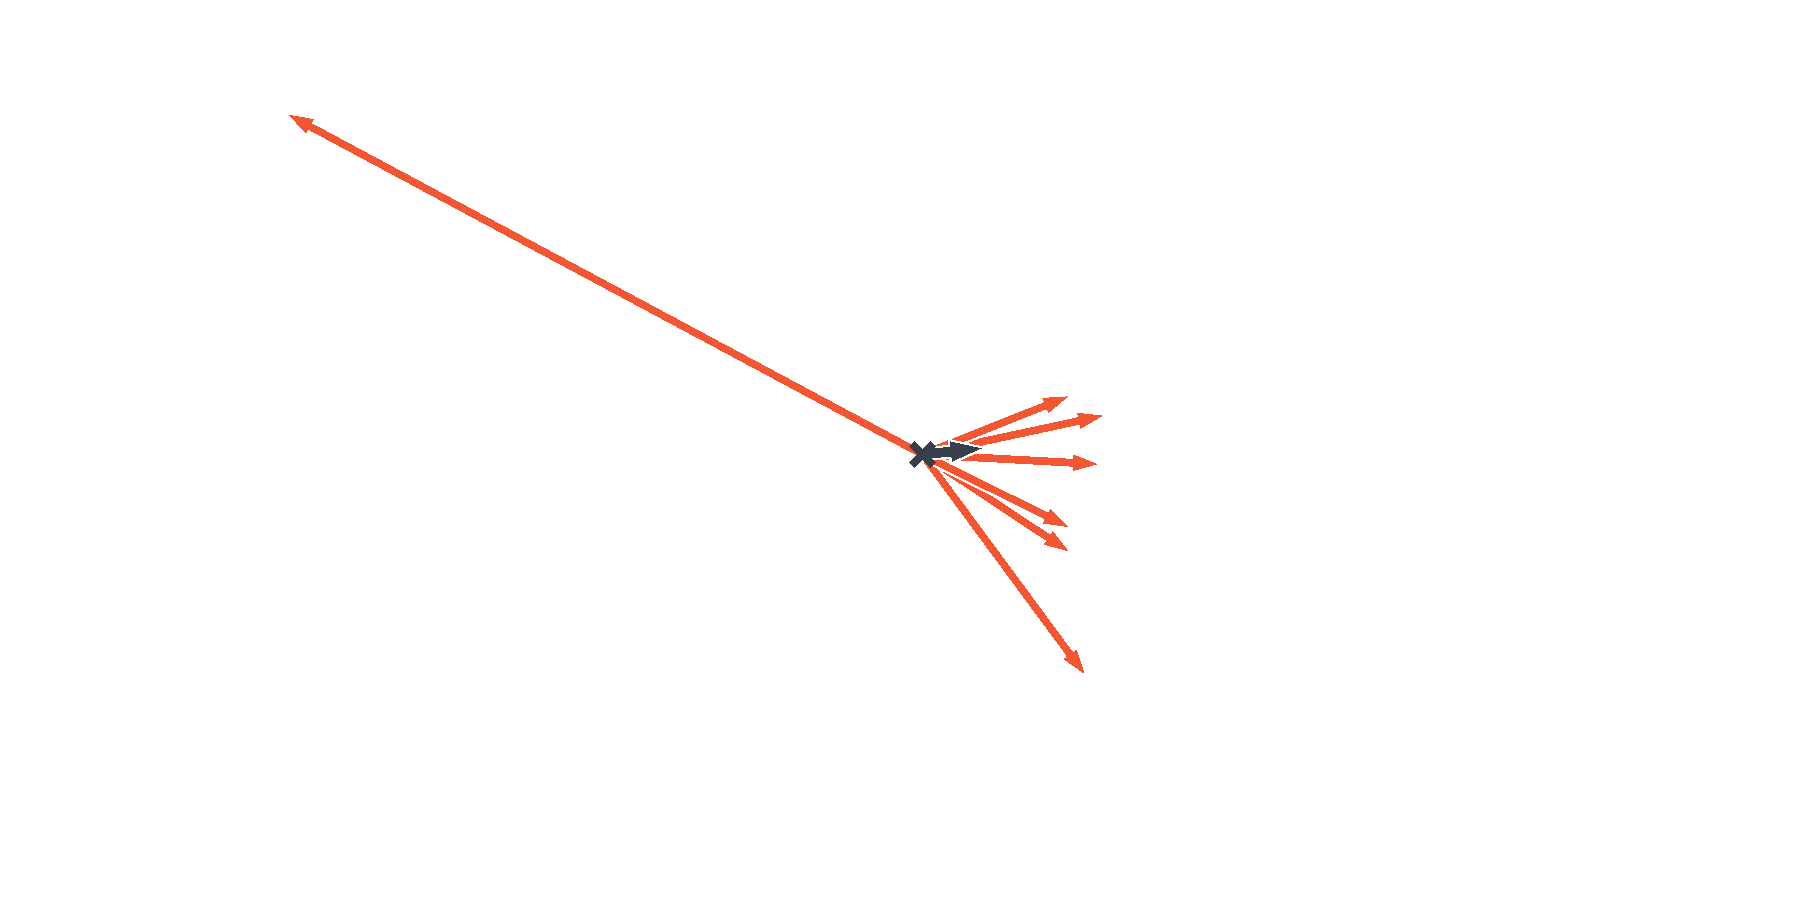
\includegraphics[width=\linewidth, trim={4.8cm 3.8cm 11.3cm 1.9cm}, clip]{../repos/backpack-paper/code/animations/differential-privacy/dp_frame_0}
    \caption{Individual gradients}\label{subfig:background::DifferentialPrivacy1}
  \end{subfigure}
  \begin{subfigure}{0.495\linewidth}
    % trim={<left> <lower> <right> <upper>}, clip
    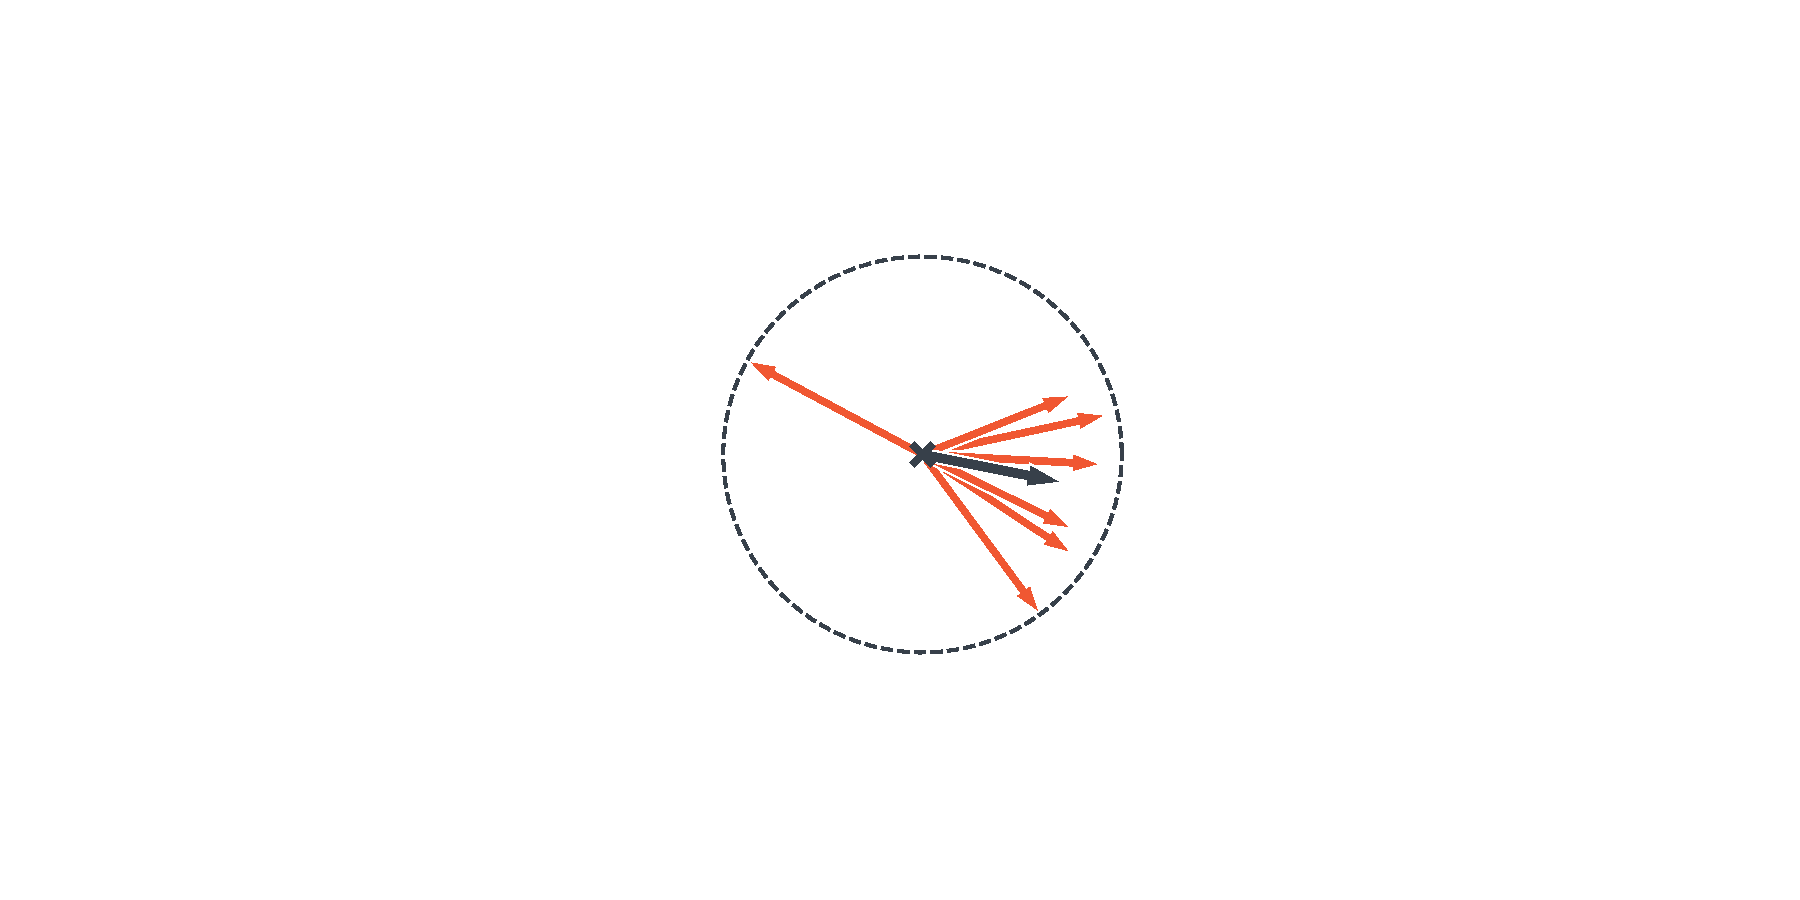
\includegraphics[width=\linewidth, trim={4.8cm 3.8cm 11.3cm 1.9cm}, clip]{../repos/backpack-paper/code/animations/differential-privacy/dp_frame_4}
    \caption{Clipped individual
      gradients}\label{subfig:background::DifferentialPrivacy2}
  \end{subfigure}
  \caption{\textbf{(Sketch) DP-SGD requires access to per-sample gradients.}
    \subfigref{subfig:background::DifferentialPrivacy1} The average gradient
    (black arrow) might be dominated by the per-sample gradients (orange arrows)
    of a small number of data. Adversaries might use this to extract potentially
    sensitive information about that data.
    \subfigref{subfig:background::DifferentialPrivacy2} Clipping per-sample
    gradients before averaging them limits the influence of individual data. The
    dashed circle's radius corresponds to the privacy threshold $C$.
  }\label{fig:background::DifferentialPrivacy}
\end{figure}

One prominent example for deep learning is differentially-private SGD
(DP-SGD)~\cite[Algorithm 1]{abadi2016deep}, which uses a negative average of
processed individual gradients over a mini-batch. To bound the influence of
individual data, per-sample gradients whose norm exceeds a specific threshold
$C$ are clipped back to norm $C$ (\Cref{fig:background::DifferentialPrivacy}),
\begin{align*}
  \vgtilde_n(\vtheta_t)
  =
  \frac{
  \vg_n(\vtheta_t)
  }{
  \max\left(
  1,
  \frac{\lVert \vg_n(\vtheta_t) \rVert_2}{C}
  \right)
  }\,.
\end{align*}
Gaussian noise of scale $\sigma$ is then added to each gradient,
\begin{align*}
  \vghat_n(\vtheta_t)
  =
  \vgtilde_n(\vtheta_t) + \vepsilon_n\,,
  \qquad
  \vepsilon_n \sim \gN(\vzero, {(\sigma C)}^2 \mI)\,.
\end{align*}
DP-SGD performs the update rule of SGD, with $\vg_n$ replaced by
$\vghat_n$,
\begin{align*}
  \vtheta_{t+1}
  =
  \vtheta_t
  -
  \eta_t
  \frac{1}{|\sB|}
  \sum_{(\vx_n,\vy_n) \in \sB}
  \vghat_n(\vtheta_t)\,.
\end{align*}
This requires access to per-sample gradient norms $\{\lVert \vg_n(\vtheta_t)
\rVert_2\}_{n}$.

\subsection{Importance Sampling}

\marginnote[*-22]{
  \begin{center}
    \pgfkeys{/pgfplots/BackPACKImportanceSamplingMNIST/.style={
    xmin = -0.02,
    xmax = 1.02,
    xtick={0, 1},
    xticklabels = {0, max},
    xlabel={$\lVert \nabla_{\vtheta}\ell_{n} \rVert_2$},
    scaled y ticks=real:50000,
    y tick label style={
      /pgf/number format/.cd,
      fixed,
      fixed zerofill,
      precision=2,
      /tikz/.cd
    },
    ytick scale label code/.code={$\cdot |\sD_{\text{train}}|$},
    ylabel = {},
    width = 1.15\linewidth,
    height = 0.9\linewidth,
    every axis plot/.append style={line width = 1.5pt},
    axis line style = black,
    tick pos = left,
    xtick align = inside,
    ytick align = inside,
    xmajorticks = true,
    ymajorticks = true,
    ylabel near ticks,
    xlabel near ticks,
    xticklabel style = {font = \footnotesize},
    xlabel style = {font = \footnotesize},
    yticklabel style = {font = \footnotesize},
    ylabel style = {font = \footnotesize},
    title style = {font = \footnotesize},
    grid = major,
    grid style = {dashed},
    legend cell align = left,
    legend style = {
      fill opacity = 0,
      text opacity = 0,
      draw opacity = 0,
      font = \footnotesize,
    },
  }
}

%%% Local Variables:
%%% mode: latex
%%% TeX-master: "../../thesis"
%%% End:

    \captionsetup[sub]{labelformat=parens}
    \begingroup
    \captionsetup{type=figure}
    \begin{subfigure}{\linewidth}
      \caption{Epoch 0, train accuracy 9.83\%}
      \vspace{-1ex}
      \pgfkeys{/pgfplots/zmystyle/.style={
          BackPACKImportanceSamplingMNIST,
          xlabel = \empty,
          xticklabel style = {opacity = 0},
        }
      }
      \tikzexternalenable
      % This file was created by tikzplotlib v0.9.0.
\begin{tikzpicture}

\definecolor{color0}{rgb}{0.941176470588235,0.341176470588235,0.196078431372549}

\begin{axis}[
axis line style={white!80!black},
legend cell align={left},
legend style={fill opacity=0.8, draw opacity=1, text opacity=1, draw=white!80!black},
tick pos=left,
x grid style={white!80!black},
xmin=0.180960892984677, xmax=1.03900186223882,
xtick style={color=gray},
xtick={0.1,0.2,0.3,0.4,0.5,0.6,0.7,0.8,0.9,1,1.1},
xticklabels={0.1,0.2,0.3,0.4,0.5,0.6,0.7,0.8,0.9,1.0,1.1},
y grid style={white!80!black},
ymin=0, ymax=3290.7,
ytick style={color=gray},
zmystyle
]
\draw[draw=white,fill=color0] (axis cs:0.219962755223502,0) rectangle (axis cs:0.235563500119032,4);
\addlegendimage{ybar,ybar legend,draw=white,fill=color0};
\addlegendentry{\ Epoch: 00, accuracy: 09.83\%}

\draw[draw=white,fill=color0] (axis cs:0.235563500119032,0) rectangle (axis cs:0.251164245014562,7);
\draw[draw=white,fill=color0] (axis cs:0.251164245014562,0) rectangle (axis cs:0.266764989910092,25);
\draw[draw=white,fill=color0] (axis cs:0.266764989910092,0) rectangle (axis cs:0.282365734805622,43);
\draw[draw=white,fill=color0] (axis cs:0.282365734805622,0) rectangle (axis cs:0.297966479701152,79);
\draw[draw=white,fill=color0] (axis cs:0.297966479701152,0) rectangle (axis cs:0.313567224596682,139);
\draw[draw=white,fill=color0] (axis cs:0.313567224596682,0) rectangle (axis cs:0.329167969492212,265);
\draw[draw=white,fill=color0] (axis cs:0.329167969492212,0) rectangle (axis cs:0.344768714387742,394);
\draw[draw=white,fill=color0] (axis cs:0.344768714387742,0) rectangle (axis cs:0.360369459283272,573);
\draw[draw=white,fill=color0] (axis cs:0.360369459283272,0) rectangle (axis cs:0.375970204178802,792);
\draw[draw=white,fill=color0] (axis cs:0.375970204178802,0) rectangle (axis cs:0.391570949074331,1008);
\draw[draw=white,fill=color0] (axis cs:0.391570949074332,0) rectangle (axis cs:0.407171693969862,1279);
\draw[draw=white,fill=color0] (axis cs:0.407171693969862,0) rectangle (axis cs:0.422772438865392,1519);
\draw[draw=white,fill=color0] (axis cs:0.422772438865392,0) rectangle (axis cs:0.438373183760921,1738);
\draw[draw=white,fill=color0] (axis cs:0.438373183760921,0) rectangle (axis cs:0.453973928656451,2090);
\draw[draw=white,fill=color0] (axis cs:0.453973928656451,0) rectangle (axis cs:0.469574673551981,2418);
\draw[draw=white,fill=color0] (axis cs:0.469574673551981,0) rectangle (axis cs:0.485175418447511,2540);
\draw[draw=white,fill=color0] (axis cs:0.485175418447511,0) rectangle (axis cs:0.500776163343041,2808);
\draw[draw=white,fill=color0] (axis cs:0.500776163343041,0) rectangle (axis cs:0.516376908238571,2924);
\draw[draw=white,fill=color0] (axis cs:0.516376908238571,0) rectangle (axis cs:0.531977653134101,3085);
\draw[draw=white,fill=color0] (axis cs:0.531977653134101,0) rectangle (axis cs:0.547578398029631,3063);
\draw[draw=white,fill=color0] (axis cs:0.547578398029631,0) rectangle (axis cs:0.563179142925161,3134);
\draw[draw=white,fill=color0] (axis cs:0.563179142925161,0) rectangle (axis cs:0.578779887820691,2925);
\draw[draw=white,fill=color0] (axis cs:0.578779887820691,0) rectangle (axis cs:0.594380632716221,2761);
\draw[draw=white,fill=color0] (axis cs:0.594380632716221,0) rectangle (axis cs:0.609981377611751,2560);
\draw[draw=white,fill=color0] (axis cs:0.609981377611751,0) rectangle (axis cs:0.625582122507281,2211);
\draw[draw=white,fill=color0] (axis cs:0.625582122507281,0) rectangle (axis cs:0.641182867402811,1927);
\draw[draw=white,fill=color0] (axis cs:0.641182867402811,0) rectangle (axis cs:0.656783612298341,1669);
\draw[draw=white,fill=color0] (axis cs:0.656783612298341,0) rectangle (axis cs:0.672384357193871,1476);
\draw[draw=white,fill=color0] (axis cs:0.672384357193871,0) rectangle (axis cs:0.687985102089401,1118);
\draw[draw=white,fill=color0] (axis cs:0.687985102089401,0) rectangle (axis cs:0.703585846984931,925);
\draw[draw=white,fill=color0] (axis cs:0.703585846984931,0) rectangle (axis cs:0.719186591880461,673);
\draw[draw=white,fill=color0] (axis cs:0.719186591880461,0) rectangle (axis cs:0.734787336775991,511);
\draw[draw=white,fill=color0] (axis cs:0.734787336775991,0) rectangle (axis cs:0.750388081671521,411);
\draw[draw=white,fill=color0] (axis cs:0.750388081671521,0) rectangle (axis cs:0.765988826567051,257);
\draw[draw=white,fill=color0] (axis cs:0.765988826567051,0) rectangle (axis cs:0.781589571462581,174);
\draw[draw=white,fill=color0] (axis cs:0.781589571462581,0) rectangle (axis cs:0.797190316358111,154);
\draw[draw=white,fill=color0] (axis cs:0.797190316358111,0) rectangle (axis cs:0.812791061253641,91);
\draw[draw=white,fill=color0] (axis cs:0.812791061253641,0) rectangle (axis cs:0.828391806149171,54);
\draw[draw=white,fill=color0] (axis cs:0.82839180614917,0) rectangle (axis cs:0.8439925510447,40);
\draw[draw=white,fill=color0] (axis cs:0.8439925510447,0) rectangle (axis cs:0.85959329594023,17);
\draw[draw=white,fill=color0] (axis cs:0.85959329594023,0) rectangle (axis cs:0.87519404083576,20);
\draw[draw=white,fill=color0] (axis cs:0.87519404083576,0) rectangle (axis cs:0.89079478573129,9);
\draw[draw=white,fill=color0] (axis cs:0.89079478573129,0) rectangle (axis cs:0.90639553062682,4);
\draw[draw=white,fill=color0] (axis cs:0.90639553062682,0) rectangle (axis cs:0.92199627552235,2);
\draw[draw=white,fill=color0] (axis cs:0.92199627552235,0) rectangle (axis cs:0.93759702041788,1);
\draw[draw=white,fill=color0] (axis cs:0.93759702041788,0) rectangle (axis cs:0.95319776531341,2);
\draw[draw=white,fill=color0] (axis cs:0.95319776531341,0) rectangle (axis cs:0.96879851020894,0);
\draw[draw=white,fill=color0] (axis cs:0.96879851020894,0) rectangle (axis cs:0.98439925510447,0);
\draw[draw=white,fill=color0] (axis cs:0.98439925510447,0) rectangle (axis cs:1,1);
\end{axis}

\end{tikzpicture}

      \tikzexternaldisable
      \vspace{-6ex}
    \end{subfigure}
    \begin{subfigure}{\linewidth}
      \caption{Epoch 2, train accuracy 83.4\%}
      \vspace{-1ex}
      \pgfkeys{/pgfplots/zmystyle/.style={
          BackPACKImportanceSamplingMNIST,
          xlabel = \empty,
          xticklabel style = {opacity = 0},
        }
      }
      \tikzexternalenable
      % This file was created by tikzplotlib v0.9.0.
\begin{tikzpicture}

\definecolor{color0}{rgb}{0.941176470588235,0.341176470588235,0.196078431372549}

\begin{axis}[
axis line style={white!80!black},
legend cell align={left},
legend style={fill opacity=0.8, draw opacity=1, text opacity=1, draw=white!80!black},
tick pos=left,
x grid style={white!80!black},
xmin=-0.0235874482194031, xmax=1.04874225943902,
xtick style={color=gray},
xtick={-0.2,0,0.2,0.4,0.6,0.8,1,1.2},
xticklabels={−0.2,0.0,0.2,0.4,0.6,0.8,1.0,1.2},
y grid style={white!80!black},
ymin=0, ymax=3099.6,
ytick style={color=gray},
zmystyle
]
\draw[draw=white,fill=color0] (axis cs:0.0251548112196161,0) rectangle (axis cs:0.0446517149952238,90);
\addlegendimage{ybar,ybar legend,draw=white,fill=color0};
\addlegendentry{\ Epoch: 02, accuracy: 83.40\%}

\draw[draw=white,fill=color0] (axis cs:0.0446517149952238,0) rectangle (axis cs:0.0641486187708315,293);
\draw[draw=white,fill=color0] (axis cs:0.0641486187708315,0) rectangle (axis cs:0.0836455225464392,611);
\draw[draw=white,fill=color0] (axis cs:0.0836455225464392,0) rectangle (axis cs:0.103142426322047,1523);
\draw[draw=white,fill=color0] (axis cs:0.103142426322047,0) rectangle (axis cs:0.122639330097655,1968);
\draw[draw=white,fill=color0] (axis cs:0.122639330097655,0) rectangle (axis cs:0.142136233873262,1998);
\draw[draw=white,fill=color0] (axis cs:0.142136233873262,0) rectangle (axis cs:0.16163313764887,1973);
\draw[draw=white,fill=color0] (axis cs:0.16163313764887,0) rectangle (axis cs:0.181130041424478,2001);
\draw[draw=white,fill=color0] (axis cs:0.181130041424478,0) rectangle (axis cs:0.200626945200085,2081);
\draw[draw=white,fill=color0] (axis cs:0.200626945200085,0) rectangle (axis cs:0.220123848975693,2047);
\draw[draw=white,fill=color0] (axis cs:0.220123848975693,0) rectangle (axis cs:0.239620752751301,2217);
\draw[draw=white,fill=color0] (axis cs:0.239620752751301,0) rectangle (axis cs:0.259117656526908,2397);
\draw[draw=white,fill=color0] (axis cs:0.259117656526908,0) rectangle (axis cs:0.278614560302516,2682);
\draw[draw=white,fill=color0] (axis cs:0.278614560302516,0) rectangle (axis cs:0.298111464078124,2769);
\draw[draw=white,fill=color0] (axis cs:0.298111464078124,0) rectangle (axis cs:0.317608367853731,2952);
\draw[draw=white,fill=color0] (axis cs:0.317608367853731,0) rectangle (axis cs:0.337105271629339,2754);
\draw[draw=white,fill=color0] (axis cs:0.337105271629339,0) rectangle (axis cs:0.356602175404947,2654);
\draw[draw=white,fill=color0] (axis cs:0.356602175404947,0) rectangle (axis cs:0.376099079180554,2566);
\draw[draw=white,fill=color0] (axis cs:0.376099079180554,0) rectangle (axis cs:0.395595982956162,2335);
\draw[draw=white,fill=color0] (axis cs:0.395595982956162,0) rectangle (axis cs:0.41509288673177,2063);
\draw[draw=white,fill=color0] (axis cs:0.41509288673177,0) rectangle (axis cs:0.434589790507377,1800);
\draw[draw=white,fill=color0] (axis cs:0.434589790507377,0) rectangle (axis cs:0.454086694282985,1570);
\draw[draw=white,fill=color0] (axis cs:0.454086694282985,0) rectangle (axis cs:0.473583598058593,1361);
\draw[draw=white,fill=color0] (axis cs:0.473583598058593,0) rectangle (axis cs:0.4930805018342,1056);
\draw[draw=white,fill=color0] (axis cs:0.4930805018342,0) rectangle (axis cs:0.512577405609808,891);
\draw[draw=white,fill=color0] (axis cs:0.512577405609808,0) rectangle (axis cs:0.532074309385416,730);
\draw[draw=white,fill=color0] (axis cs:0.532074309385416,0) rectangle (axis cs:0.551571213161023,567);
\draw[draw=white,fill=color0] (axis cs:0.551571213161023,0) rectangle (axis cs:0.571068116936631,437);
\draw[draw=white,fill=color0] (axis cs:0.571068116936631,0) rectangle (axis cs:0.590565020712239,347);
\draw[draw=white,fill=color0] (axis cs:0.590565020712239,0) rectangle (axis cs:0.610061924487846,290);
\draw[draw=white,fill=color0] (axis cs:0.610061924487846,0) rectangle (axis cs:0.629558828263454,207);
\draw[draw=white,fill=color0] (axis cs:0.629558828263454,0) rectangle (axis cs:0.649055732039062,195);
\draw[draw=white,fill=color0] (axis cs:0.649055732039062,0) rectangle (axis cs:0.66855263581467,138);
\draw[draw=white,fill=color0] (axis cs:0.668552635814669,0) rectangle (axis cs:0.688049539590277,106);
\draw[draw=white,fill=color0] (axis cs:0.688049539590277,0) rectangle (axis cs:0.707546443365885,67);
\draw[draw=white,fill=color0] (axis cs:0.707546443365885,0) rectangle (axis cs:0.727043347141493,54);
\draw[draw=white,fill=color0] (axis cs:0.727043347141493,0) rectangle (axis cs:0.7465402509171,35);
\draw[draw=white,fill=color0] (axis cs:0.7465402509171,0) rectangle (axis cs:0.766037154692708,35);
\draw[draw=white,fill=color0] (axis cs:0.766037154692708,0) rectangle (axis cs:0.785534058468316,13);
\draw[draw=white,fill=color0] (axis cs:0.785534058468316,0) rectangle (axis cs:0.805030962243923,16);
\draw[draw=white,fill=color0] (axis cs:0.805030962243923,0) rectangle (axis cs:0.824527866019531,14);
\draw[draw=white,fill=color0] (axis cs:0.824527866019531,0) rectangle (axis cs:0.844024769795139,4);
\draw[draw=white,fill=color0] (axis cs:0.844024769795139,0) rectangle (axis cs:0.863521673570746,5);
\draw[draw=white,fill=color0] (axis cs:0.863521673570746,0) rectangle (axis cs:0.883018577346354,2);
\draw[draw=white,fill=color0] (axis cs:0.883018577346354,0) rectangle (axis cs:0.902515481121962,2);
\draw[draw=white,fill=color0] (axis cs:0.902515481121962,0) rectangle (axis cs:0.922012384897569,1);
\draw[draw=white,fill=color0] (axis cs:0.922012384897569,0) rectangle (axis cs:0.941509288673177,0);
\draw[draw=white,fill=color0] (axis cs:0.941509288673177,0) rectangle (axis cs:0.961006192448785,0);
\draw[draw=white,fill=color0] (axis cs:0.961006192448785,0) rectangle (axis cs:0.980503096224392,2);
\draw[draw=white,fill=color0] (axis cs:0.980503096224392,0) rectangle (axis cs:1,1);
\end{axis}

\end{tikzpicture}

      \tikzexternaldisable
      \vspace{-6ex}
    \end{subfigure}
    \begin{subfigure}{\linewidth}
      \caption{Epoch 49, train accuracy 90.5\%}
      \vspace{-1ex}
      \pgfkeys{/pgfplots/zmystyle/.style={
          BackPACKImportanceSamplingMNIST,
        }
      }
      \tikzexternalenable
      % This file was created by tikzplotlib v0.9.0.
\begin{tikzpicture}

\definecolor{color0}{rgb}{0.941176470588235,0.341176470588235,0.196078431372549}

\begin{axis}[
axis line style={white!80!black},
legend cell align={left},
legend style={fill opacity=0.8, draw opacity=1, text opacity=1, draw=white!80!black},
tick pos=left,
x grid style={white!80!black},
xmin=-0.0499953146370904, xmax=1.04999977688748,
xtick style={color=gray},
xtick={-0.2,0,0.2,0.4,0.6,0.8,1,1.2},
xticklabels={−0.2,0.0,0.2,0.4,0.6,0.8,1.0,1.2},
y grid style={white!80!black},
ymin=0, ymax=20526.45,
ytick style={color=gray},
zmystyle
]
\draw[draw=white,fill=color0] (axis cs:4.46225039008562e-06,0) rectangle (axis cs:0.0200043730053823,19549);
\addlegendimage{ybar,ybar legend,draw=white,fill=color0};
\addlegendentry{\ Epoch: 49, accuracy: 90.49\%}

\draw[draw=white,fill=color0] (axis cs:0.0200043730053823,0) rectangle (axis cs:0.0400042837603745,7018);
\draw[draw=white,fill=color0] (axis cs:0.0400042837603745,0) rectangle (axis cs:0.0600041945153667,4100);
\draw[draw=white,fill=color0] (axis cs:0.0600041945153667,0) rectangle (axis cs:0.0800041052703589,2853);
\draw[draw=white,fill=color0] (axis cs:0.0800041052703589,0) rectangle (axis cs:0.100004016025351,2112);
\draw[draw=white,fill=color0] (axis cs:0.100004016025351,0) rectangle (axis cs:0.120003926780343,1752);
\draw[draw=white,fill=color0] (axis cs:0.120003926780343,0) rectangle (axis cs:0.140003837535335,1514);
\draw[draw=white,fill=color0] (axis cs:0.140003837535335,0) rectangle (axis cs:0.160003748290328,1212);
\draw[draw=white,fill=color0] (axis cs:0.160003748290328,0) rectangle (axis cs:0.18000365904532,1032);
\draw[draw=white,fill=color0] (axis cs:0.18000365904532,0) rectangle (axis cs:0.200003569800312,866);
\draw[draw=white,fill=color0] (axis cs:0.200003569800312,0) rectangle (axis cs:0.220003480555304,810);
\draw[draw=white,fill=color0] (axis cs:0.220003480555304,0) rectangle (axis cs:0.240003391310296,694);
\draw[draw=white,fill=color0] (axis cs:0.240003391310296,0) rectangle (axis cs:0.260003302065289,661);
\draw[draw=white,fill=color0] (axis cs:0.260003302065289,0) rectangle (axis cs:0.280003212820281,594);
\draw[draw=white,fill=color0] (axis cs:0.280003212820281,0) rectangle (axis cs:0.300003123575273,537);
\draw[draw=white,fill=color0] (axis cs:0.300003123575273,0) rectangle (axis cs:0.320003034330265,521);
\draw[draw=white,fill=color0] (axis cs:0.320003034330265,0) rectangle (axis cs:0.340002945085257,462);
\draw[draw=white,fill=color0] (axis cs:0.340002945085257,0) rectangle (axis cs:0.36000285584025,415);
\draw[draw=white,fill=color0] (axis cs:0.36000285584025,0) rectangle (axis cs:0.380002766595242,391);
\draw[draw=white,fill=color0] (axis cs:0.380002766595242,0) rectangle (axis cs:0.400002677350234,384);
\draw[draw=white,fill=color0] (axis cs:0.400002677350234,0) rectangle (axis cs:0.420002588105226,341);
\draw[draw=white,fill=color0] (axis cs:0.420002588105226,0) rectangle (axis cs:0.440002498860218,325);
\draw[draw=white,fill=color0] (axis cs:0.440002498860218,0) rectangle (axis cs:0.460002409615211,271);
\draw[draw=white,fill=color0] (axis cs:0.460002409615211,0) rectangle (axis cs:0.480002320370203,261);
\draw[draw=white,fill=color0] (axis cs:0.480002320370203,0) rectangle (axis cs:0.500002231125195,230);
\draw[draw=white,fill=color0] (axis cs:0.500002231125195,0) rectangle (axis cs:0.520002141880187,188);
\draw[draw=white,fill=color0] (axis cs:0.520002141880187,0) rectangle (axis cs:0.54000205263518,160);
\draw[draw=white,fill=color0] (axis cs:0.54000205263518,0) rectangle (axis cs:0.560001963390172,123);
\draw[draw=white,fill=color0] (axis cs:0.560001963390172,0) rectangle (axis cs:0.580001874145164,129);
\draw[draw=white,fill=color0] (axis cs:0.580001874145164,0) rectangle (axis cs:0.600001784900156,92);
\draw[draw=white,fill=color0] (axis cs:0.600001784900156,0) rectangle (axis cs:0.620001695655148,73);
\draw[draw=white,fill=color0] (axis cs:0.620001695655148,0) rectangle (axis cs:0.64000160641014,67);
\draw[draw=white,fill=color0] (axis cs:0.64000160641014,0) rectangle (axis cs:0.660001517165133,50);
\draw[draw=white,fill=color0] (axis cs:0.660001517165133,0) rectangle (axis cs:0.680001427920125,32);
\draw[draw=white,fill=color0] (axis cs:0.680001427920125,0) rectangle (axis cs:0.700001338675117,26);
\draw[draw=white,fill=color0] (axis cs:0.700001338675117,0) rectangle (axis cs:0.720001249430109,31);
\draw[draw=white,fill=color0] (axis cs:0.720001249430109,0) rectangle (axis cs:0.740001160185101,15);
\draw[draw=white,fill=color0] (axis cs:0.740001160185102,0) rectangle (axis cs:0.760001070940094,9);
\draw[draw=white,fill=color0] (axis cs:0.760001070940094,0) rectangle (axis cs:0.780000981695086,7);
\draw[draw=white,fill=color0] (axis cs:0.780000981695086,0) rectangle (axis cs:0.800000892450078,6);
\draw[draw=white,fill=color0] (axis cs:0.800000892450078,0) rectangle (axis cs:0.82000080320507,1);
\draw[draw=white,fill=color0] (axis cs:0.82000080320507,0) rectangle (axis cs:0.840000713960062,1);
\draw[draw=white,fill=color0] (axis cs:0.840000713960062,0) rectangle (axis cs:0.860000624715055,0);
\draw[draw=white,fill=color0] (axis cs:0.860000624715055,0) rectangle (axis cs:0.880000535470047,2);
\draw[draw=white,fill=color0] (axis cs:0.880000535470047,0) rectangle (axis cs:0.900000446225039,0);
\draw[draw=white,fill=color0] (axis cs:0.900000446225039,0) rectangle (axis cs:0.920000356980031,0);
\draw[draw=white,fill=color0] (axis cs:0.920000356980031,0) rectangle (axis cs:0.940000267735023,2);
\draw[draw=white,fill=color0] (axis cs:0.940000267735023,0) rectangle (axis cs:0.960000178490016,0);
\draw[draw=white,fill=color0] (axis cs:0.960000178490016,0) rectangle (axis cs:0.980000089245008,0);
\draw[draw=white,fill=color0] (axis cs:0.980000089245008,0) rectangle (axis cs:1,1);
\end{axis}

\end{tikzpicture}

      \tikzexternaldisable
      \vspace{-2ex}
    \end{subfigure}
    \endgroup
    \captionof{figure}{\textbf{Importance distribution of samples during
        training.} Importance is measured by individual gradient $L_{2}$ norms,
      computed with \backpack (\Cref{chap:backpack}). As training proceeds and
      more examples are correctly classified and become ``unimportant''.
      Details: logistic regression on \mnist, trained with \sgd, $|\sB| = 128$,
      and learning rate $0.005$.}\label{fig:background::SquaredL2Norms}
  \end{center}
}

A hypothesis about learning in ML is that the model first learns to correctly
predict ``easy'' examples. Only in later phases are the ``difficult'' examples
learned. Using these harder examples more frequently for training might help
speed up the learning procedure. Put differently, some data matter more at
certain stages of training than other, which is quantified through a measure of
importance. Importance sampling realizes this idea of selecting important data
more frequently. It does so by adapting the sampling procedure for mini-batches
to reduce the gradient variance, which beneficially influences the convergence
of stochastic first-order methods like \sgd, and therefore speeds up training. A
common strategy is to weight the importance of samples by the per-sample $L_2$
norm
(\Cref{eq:background::importanceSamplingOptimalDistribution,fig:background::SquaredL2Norms}).

As a starting point to see how the sampling procedure affects optimization,
consider the generalization of uniform sampling from
\Cref{sec:background::MiniBatching} for $|\sB| = 1$. At training iteration $t$,
a sample $n_t\sim p_t(n_t)$ is drawn from a current sampling distribution
$p_t(n_t)$ over $\{1, \dots, |\sD|\}$. \sgd with a learning rate $\eta$ uses the
unbiased gradient estimator\sidenote[][0\baselineskip]{%
  For uniform sampling $p_{t}(n_{t}) = \nicefrac{1}{|\sD|}$, which is the most
  common case in practice, the scaling factor cancels and yields the commonly
  used gradient estimator that would be used by ``normal'' \sgd with $|\sB| =
  1$.%
}
\begin{subequations}
  \begin{align}\label{eq:background::gradientEstimator}
    \vghat_{n_t}(\vtheta_t)
    &:=
      \frac{1}{|\sD| p_t(n_t)}
      \grad{\vtheta_t}\ell_{n_t}(\vtheta_t)
      \shortintertext{with}
      \E_{n_t \sim p_t(n_t)}\left[ \vghat_{n_t}(\vtheta_t) \right]
    &=
      \frac{1}{|\sD|} \sum_{(\vx_n, \vy_n) \in \sD}
      \grad{\vtheta_t} \ell_{n_t}(\vtheta_t)
      = \vg_{\sD}(\vtheta_t)
      \shortintertext{to update the parameters}
      \label{eq:background::gradientDescentSampled}
      \vtheta_{t+1} &= \vtheta_t - \eta \vghat_{n_t}(\vtheta_{t})\,.
  \end{align}
\end{subequations}
Using a non-uniform distribution over stochastic gradients would introduce bias
in the update, so in importance sampling the samples are weighted by their
probability of being selected to undo the bias. The distribution can then be
tuned to minimize the variance of the estimator and improve performance: one can
assess convergence of \Cref{eq:background::gradientDescentSampled} through the
progress towards the minimizer $\vtheta_{\star}$ in terms of squared $L_2$
distance~\cite{wang2017accelerating,katharopoulos2018samples},
\begin{subequations}
  \begin{align}
    \lVert \vtheta_{t} - \vtheta_{\star} \rVert_2^{2}
    -
    \lVert \vtheta_{t+1} - \vtheta_{\star} \rVert_2^{2}\,.
  \end{align}
  In expectation, this measure of convergence depends on the gradient estimator's
  variance (more specifically, its trace),
  \begin{align}
    \begin{split}
      \E_{n_t}
      &\left[
        \lVert \vtheta_{t} - \vtheta_{\star} \rVert_2^2
        -
        \lVert \vtheta_{t+1} - \vtheta_{\star} \rVert_2^2
        \right]
      \\
      &=
        \E_{n_t}\left[
        \lVert \vtheta_{t} - \vtheta_{\star} \rVert_2^{2}
        -
        \lVert \vtheta_{t} - \vtheta_{\star} - \eta \vghat_{n_t}  \rVert_2^{2}
        \right]
      \\
      &=
        \E_{n_t}\left[
        2 \eta \left(
        \vtheta_{t} - \vtheta_{\star}
        \right)^{\top} \vghat_{n_t}
        - \eta^2 \vghat_{n_t}^{\top} \vghat_{n_t}
        \right]
      \\
      &=
        2 \eta \left(
        \vtheta_{t} - \vtheta_{\star}
        \right)^{\top}
        \vg_{\sD}
        -
        \eta^2 \E_{n_t}\left[
        \lVert \vghat_{n_t} \rVert_2^2
        \right]
      \\
      &=
        2 \eta \left(
        \vtheta_{t} - \vtheta_{\star}
        \right)^{\top}
        \vg_{\sD}
        - \eta^2 \lVert \vg_{\sD} \rVert_2^2
        -
        \eta^2 \E_{n_t}\left[
        \lVert \vghat_{n_t} - \vg_{\sD} \rVert_2^2
        \right]
      \\
      &=
        2 \eta \left(
        \vtheta_{t} - \vtheta_{\star}
        \right)^{\top}
        \vg_{\sD}
        - \eta^2 \lVert \vg_{\sD} \rVert_2^2
        -
        \eta^2 \Tr\left\{
        \Var_{n_t}\left[\vghat_{n_t}
        \right]\right\}
    \end{split}
  \end{align}
\end{subequations}
For what follows, the intuition is that sampling affects convergence through the
variance term, and minimizing this term improves convergence. Hence, the goal is
to identify the optimal sampling via
\begin{align}\label{ex:background::findOptimalSamplingDistribution}
  \minimize_{\substack{p_t(n_t) \\ \sum_{n=1}^{|\sD|} p_t(n) = 1}}
  \Tr\left\{
  \Var_{n_t}\left[\vghat_{n_t}
  \right]\right\}
  \quad
  \Leftrightarrow
  \quad
  \minimize_{\substack{p_t(n_t) \\ \sum_{n=1}^{|\sD|} p_t(n) = 1}}
  \E_{n_t}
  \left[
  \lVert
  \vghat_{n_t}
  \rVert_2^2
  \right]
\end{align}
The solution, outlined in \Cref{ex:background::importanceSamplingDerivation}, is
\begin{align}
  \label{eq:background::importanceSamplingOptimalDistribution}
  p_t(n_t)
  =
  \frac{
  \lVert \grad{\vtheta_t}\ell_{n_t}(\vtheta_t) \rVert_2
  }{
  \sum_{n=1}^{|\sD|} \lVert \ell_{n}(\vtheta_t) \rVert_2
  }\,.
\end{align}
%
and
\marginnote[*-31]{%
  \begin{remark}[\textbf{Optimal sampling
      distribution~\cite{needell2014stochastic,zhao2015stochastic}}]\label{ex:background::importanceSamplingDerivation}
    (The iteration index $t$ is suppressed for brevity) To derive
    \Cref{eq:background::importanceSamplingOptimalDistribution}, one
    incorporates the constraint in
    \Cref{ex:background::findOptimalSamplingDistribution} via a Lagrange
    multiplier $\mu \in \sR$, writing $p(n)$ as $|\sD|$-dimensional vector
    $\vp$. Expanding $\vghat$ with \Cref{eq:background::gradientEstimator} leads
    to,
    \begin{align*}
      A(\vp, \mu)
      &:=
        \frac{1}{|\sD|^2}
        \sum_{n=1}^{|\sD|}
        \frac{
        \lVert \grad{\vtheta}\ell_n(\vtheta)\rVert_2^2
        }{
        \evp_n
        }
      \\
      &\phantom{= } \
        +
        \mu
        \left(
        \sum_{n=1}^{|\sD|}
        \evp_n
        -1
        \right)\,.
    \end{align*}
    Setting the $\evp_n$-derivative of that to zero yields
    \begin{align*}
      \grad{\evp_n} A(\vp, \mu)
      &=
        -
        \frac{
        \lVert \grad{\vtheta}\ell_n(\vtheta)\rVert_2^2
        }{
        |\sD|^2
        \evp_n^2
        }
        + \mu
        \overset{!}{=} 0
      \\
      \implies
      \quad
      \evp_n
      &=
        \frac{
        \lVert \grad{\vtheta}\ell_n(\vtheta)\rVert_2
        }{
        \sqrt{\mu}
        }\,,
    \end{align*}
    using that all elements $\evp_n \in (0; 1)$ of $\vp$. Inserting into
    $A$ gives
    \begin{align*}
      A(\mu)
      =
      \frac{2}{|\sD|}
      \sqrt{\mu}
      \sum_{n=1}^{|\sD|}
      \lVert \grad{\vtheta}\ell_n(\vtheta)\rVert_2
      -
      \mu
    \end{align*}
    Setting the $\mu$-derivative to zero yields
    \begin{align*}
      \grad{\mu}A(\mu)
      &=
        \frac{1}{|\sD| \sqrt{\mu}}
        \sum_{n=1}^{|\sD|}
        \lVert \grad{\vtheta}\ell_n(\vtheta)\rVert_2
        - 1
        \overset{!}{=} 0
      \\
      \implies
      \quad
      \sqrt{\mu}
      &=
        \frac{1}{|\sD|}
        \sum_{n=1}^{|\sD|}
        \lVert \grad{\vtheta}\ell_n(\vtheta)\rVert_2
    \end{align*}
    This then leads to
    \begin{align*}
      \evp_n
      =
      \frac{
      \lVert \grad{\vtheta}\ell_n(\vtheta)\rVert_2
      }{
      \sum_{n=1}^{|\sD|}
      \lVert \grad{\vtheta}\ell_n(\vtheta)\rVert_2
      }
    \end{align*}
    which equals \Cref{eq:background::importanceSamplingOptimalDistribution}
    when switching back notation and introducing the iteration count.
  \end{remark}
} %
depends on individual gradient $L_2$ norms in the entire dataset. Samples with
higher importance, \ie gradient norm, are drawn more frequently. Because
computing the sampling distribution requires a sweep over all data, practical
versions further approximate
\Cref{eq:background::importanceSamplingOptimalDistribution}, \eg by relaxing the
optimization through bounds that are easier to compute, or updating the
distribution only every few iterations~\cite{katharopoulos2018samples}.

%%% Local Variables:
%%% mode: latex
%%% TeX-master: "../thesis"
%%% End:


%%% Local Variables:
%%% mode: latex
%%% TeX-master: "../thesis"
%%% End:

% ---------------------------------
% MAIN WORK
% ---------------------------------

\pagelayout{wide} % disable margins
\part{Backpropagation Beyond the Gradient}\label{part:papers}
\pagelayout{margin} % restore margins

\setchapterpreamble[u]{\margintoc}
\chapter{Modular Block-diagonal Curvature Approximations for Feedforward
  Architectures}\label{chap:hbp}
\subsubsection{Abstract}

We propose a modular extension of backpropagation for the computation of
block-diagonal approximations to various curvature matrices of the training
objective (in particular, the Hessian, generalized Gauss-Newton, and
positive-curvature Hessian). The approach reduces the otherwise tedious manual
derivation of these matrices into local modules, and is easy to integrate into
existing machine learning libraries. Moreover, we develop a compact notation
derived from matrix differential calculus. We outline different strategies
applicable to our method. They subsume recently-proposed block-diagonal
approximations as special cases, and are extended to convolutional neural
networks in this work.

\marginnote{
  \begin{center}
    Code and experiments available at the Github repository
    \href{https://github.com/f-dangel/hbp}{\texttt{f-dangel/hbp}}
  \end{center}
  \begin{center}
    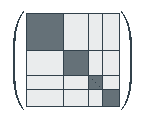
\includegraphics[height=0.8\linewidth]{../repos/hbp-paper/doc/aistats_talk/logo/hbp_logo}
  \end{center}
}

\section{Introduction}
Gradient backpropagation is the central computational operation of contemporary
deep learning. Its modular structure allows easy extension across network
architectures, and thus automatic computation of gradients given the
computational graph of the forward pass \citep[for a review,
see][]{baydin2018automatic}. But optimization using only the first-order
information of the objective's gradient can be unstable and slow, due to
``vanishing'' or ``exploding'' behaviour of the gradient. Incorporating
curvature, second-order methods can avoid such scaling issues and converge in
fewer iterations. Such methods locally approximate the objective function $\gL$ by
a quadratic
\begin{math}
  \gL(\vtheta) + \grad{\vtheta}\gL(\vtheta)^\top (\vtheta_\star - \vtheta)
  + \nicefrac{1}{2} (\vtheta_\star - \vtheta)^\top \mC(\vtheta) (\vtheta_\star - \vtheta)
\end{math}
around the current location $\vtheta$, using the gradient
$\nabla_{\vtheta}\gL(\vtheta) = \nicefrac{\partial \gL(\vtheta)}{\partial
  \vtheta}$ and a positive semi-definite (PSD) curvature matrix
$\mC(\vtheta)$---the Hessian of $\gL$ or approximations thereof. The quadratic
is minimized by
\begin{align}
  \label{hbp::equ:NewtonUpdate}
  \vtheta_\star = \vtheta
  + \Delta \vtheta
  \quad
  \text{with}
  \quad \Delta \vtheta = -\mC(\vtheta)^{-1} \grad{\vtheta}\gL\,.
\end{align}
Computing the update step requires solving the linear system $\mC(\vtheta)
\Delta \vtheta = -\grad{\vtheta}\gL$. To accomplish this task, providing a
matrix-vector multiplication with the curvature matrix $\mC(\vtheta)$ is
sufficient.

\subsubsection{Approaches to Second-order Optimization}

For some curvature matrices, exact multiplication can be performed at the cost
of one backward pass by automatic differentiation
\citep{pearlmutter1994fast,schraudolph2002fast}. This \emph{matrix-free}
formulation can then be leveraged to solve \Cref{hbp::equ:NewtonUpdate} using
iterative solvers such as conjugate gradients~(CG)~\citep{martens2010deep}.
However, since this linear solver can still require multiple iterations, the
increased per-iteration progress of the resulting optimizer might be compensated
by increased computational cost. Recently, a parallel version of Hessian-free
optimization was proposed in~\citep{zhang2017blockdiagonal}, which only
considers the content of Hessian sub-blocks along the diagonal. Reducing the
Hessian to a block diagonal allows for parallelization, tends to lower the
required number of CG iterations, and seems to improve the optimizer's
performance.

\begin{figure*}[t]
  \centering\resizebox{\linewidth}{!}{
    \tikzexternalenable
    {\footnotesize
      % basic setting of a fully-connected neural network with data flow for
% forward pass

\begin{tikzpicture}
  % first two layers
  \node (in1)
  [inner sep=0]
  {\tikz \drawMessagesWithArrows{$\vz^{(0)}$}{ }{ }{\hNodeDistance};};
  \node (layer1)
  [anchor=south west, inner sep=0]
  at (in1.south east)
  {\tikz \drawModuleWithParams{$f^{(1)}_{\vtheta^{(1)}}$}{16}{$\vtheta^{(1)}$}{$\grad{\vtheta^{(1)}}\ell$}{ };};
  \node (out1)
  [inner sep=0, anchor=south west]
  at (layer1.south east)
  {\tikz \drawMessagesWithArrows{$\vz^{(1)}$}{$\grad{\vz^{(1)}}\ell$}{ }{\hNodeDistance};};
  \node (layer2)
  [inner sep=0pt, anchor=south west]
  at (out1.south east)
  {\tikz\drawModuleNoParams{$f^{(2)}$}{5};};

  % third layer and dots
  \node (in2)
  [inner sep=0, anchor=south west]
  at (layer2.south east)
  {\tikz \drawMessagesWithArrows{$\vz^{(2)}$}{$\grad{\vz^{(2)}}\ell$}{ }{\hNodeDistance};};
  \node (layer3)
  [anchor=south west, inner sep=0]
  at (in2.south east)
  {\tikz \drawModuleWithParams{$f^{(3)}_{\vtheta^{(3)}}$}{16}{$\vtheta^{(3)}$}{$\grad{\vtheta^{(3)}}\ell$}{ };};
  \node (out3)
  [inner sep=0, anchor=south west]
  at (layer3.south east)
  {\tikz \drawMessagesWithArrows{$\vz^{(3)}$}{$\grad{\vz^{(3)}}\ell$}{ }{\hNodeDistance};};
  \node (layer4)
  [inner sep=0pt, anchor=south west]
  at (out3.south east)
  {\tikz\drawModuleNoParams{$f^{(4)}$}{5};};

  % last layer after dots
  \node (dots)
  [xshift=2ex, inner sep=0pt, anchor=west]
  at (layer4.east)
  {$\dots$};
  \node (layer5)
  [xshift=12ex, anchor=south west, inner sep=0]
  at (out3.south east)
  {\tikz \drawModuleWithParams{$f^{(L)}_{\vtheta^{(L)}}$}{16}{$\vtheta^{(L)}$}{$\grad{\vtheta^{(L)}}\ell$}{ };};
  \node (out4)
  [inner sep=0, anchor=south west]
  at (layer5.south east)
  {\tikz \drawMessagesWithArrows{$\vz^{(L)}$}{$\grad{\vz^{(L)}}\ell$}{ }{\hNodeDistance};};

  % loss layer
  \node (lossLayer)
  [inner sep=0pt, anchor=south west]
  at (out4.south east)
  {\tikz\drawModuleNoParams{$\ell$}{5};};
  \node (loss)
  [inner sep=0, anchor=south west]
  at (lossLayer.south east)
  {\tikz \drawMessagesWithArrows{$\ell$}{ }{ }{\hNodeDistance};};
\end{tikzpicture}

%%% Local Variables:
%%% mode: latex
%%% TeX-master: "../../thesis"
%%% End:

    }
    \tikzexternaldisable}
  \caption{\textbf{Standard sequential feedforward network architecture.} \Ie the
    repetition of affine transformations parameterized by $ \vtheta^{(l)} =
    ((\vec \mW^{(l)})^{\top}, \vb^{(l)\top})^{\top}$ followed by element-wise
    activations. Arrows from left to right and vice versa indicate the data flow
    during forward pass and gradient backpropagation, respectively.}
  \label{hbp::fig:setting}
\end{figure*}

There have also been attempts to compute parts of the Hessian in an iterative
fashion \citep{mizutani2008secondorder}. Storing these constituents efficiently
often requires an involved manual analysis of the Hessian's structure,
leveraging its outer-product form in many scenarios
\citep{naumov2017HessianInMatrixForm, bakker2018OuterProductStructure}. Recent
works developed different block-diagonal approximations (BDA) of curvature
matrices that provide fast
multiplication~\citep{martens2015optimizing,grosse2016kronecker,botev2017practical,wei2018bdapch}.

These works have repeatedly shown that, empirically, second-order information
can improve the training of deep learning problems. Perhaps the most important
practical hurdle to the adoption of second-order optimizers is that they tend to
be tedious to integrate in existing ML frameworks because they require manual
implementations. As efficient automated implementations have arguably been more
important for the wide-spread use of deep learning than many conceptual
advances, we aim to develop a framework that makes computation of Hessian
approximations about as easy and automated as gradient backpropagation.

\subsubsection{Contribution}

This chapter introduces a modular formalism for the computation of
block-diagonal approximations of Hessian and curvature matrices, to various
block resolutions, for feedforward neural networks. The framework unifies
previous approaches in a form that, similar to gradient backpropagation, reduces
implementation and analysis to local modules. Following the design pattern of
gradient backprop also has the advantage that this formalism can readily be
integrated into existing ML libraries, and flexibly modified for
different block groupings and approximations.

The framework consists of three principal parts:
\begin{enumerate}
\item A modular formulation for \emph{exact} computation of Hessian block
  diagonals of feedforward neural nets. We achieve a clear presentation by
  leveraging the notation of matrix differential
  calculus~\citep{magnus1999MatrixDifferentialCalculus}.
\item Projections onto the positive semi-definite cone by eliminating sources of
  concavity.
\item Backpropagation strategies to obtain (i) exact curvature matrix-vector
  products (with previously inaccessible BDAs of the Hessian) and (ii) further
  approximated multiplication routines that save computations by evaluating the
  matrix representations of intermediate quantities once, at the cost of
  additional memory consumption.
\end{enumerate}
The first two contributions can be understood as an explicit formulation of
well-known tricks for fast multiplication by curvature matrices using automatic
differentiation~\citep{pearlmutter1994fast,schraudolph2002fast}. However, we
also address a new class of curvature matrices, the positive-curvature Hessian
(PCH) introduced in~\cite{wei2018bdapch}. Our solutions to the latter two points
are generalizations of previous works~\citep{botev2017practical,wei2018bdapch}
to the fully modular case, which become accessible due to the first
contribution. They represent additional modifications to make the scheme
computationally tractable and obtain curvature approximations with desirable
properties for optimization.

%%% Local Variables:
%%% mode: latex
%%% TeX-master: "../thesis"
%%% End:


\section{Notation}\label{hbp::sec:basicSetting}
We consider feedforward neural networks $f_{\vtheta}(\vx)$ composed of $L$ modules
$f^{(l)}_{\vtheta^{(l)}}, l = 1, \ldots, L$, which can be represented as a
computational graph mapping the input $\vz^{(0)}=\vx$ to the output $\vz^{(L)}$
(\Cref{hbp::fig:setting}). A module~$f^{(l)}_{\vtheta^{(l)}}$ receives the parental
output~$\vz^{(l-1)}$, applies an operation involving the module
parameters~$\vtheta^{(l)}$, and sends the output $\vz^{(l)}$ to its child. Thus,
$f^{(l)}_{\vtheta^{(l)}}$ is of the form
\begin{math}
  \vz^{(l)} = f^{(l)}_{\vtheta^{(l)}}(\vz^{(l-1)}). %\,.
\end{math}
Typical choices include element-wise nonlinear activation without any parameters
and affine transformations $\vz^{(l)} = \mW^{(l)} \vz^{(l-1)} + \vb^{(l)}$ with
parameters given by the weights $\mW^{(l)}$ and the bias $\vb^{(l)} $. Affine and
activation modules are usually considered as a single conceptual unit, one
\emph{layer} of the network. However, for backpropagation of derivatives it is
simpler to consider them separately as two \emph{modules}.

Given the network output $\vz^{(L)}(\vx, \vtheta^{(1, \dots, L)}) = f_{\vtheta}(\vx)$ of a datum
$\vx$ with label $\vy$, the goal is to minimize the expected risk of the loss
function $\ell(\vz^{(L)}, \vy)$. Under the framework of empirical risk minimization,
the parameters are tuned to optimize the loss on the training set $\sD_{\text{train}}=
\{(\vx_{n},\vy_{n})\}_{n=1}^N$,
\begin{align}
  \label{hbp::equ:objective}
  \min_{\vtheta^{(1,\dots, L)}} \gL_{\sD_{\text{train}}}(\vtheta^{(1,\dots, L)})
  =
  \min_{\vtheta^{(1,\dots, L)}} \frac{1}{|\sD_{\text{train}}|}
  \sum_{n=1}^{N}
  \ell(f_{\vtheta}(\vx_{n}), \vy_{n})\,.
\end{align}
In practice, the objective is typically further approximated stochastically by
drawing a mini-batch $\sB \subset \sD_{\text{train}}$ from the training set. We
will treat both scenarios without further distinction, since the structure
relevant to our purposes is that \Cref{hbp::equ:objective} is an average of
terms depending on individual data points. Quantities for optimization, be it
gradients or second derivatives of the loss \wrt the network parameters, can be
processed in parallel, then averaged.

%%% Local Variables:
%%% mode: latex
%%% TeX-master: "../thesis"
%%% End:


\section{Modular Hessian Backpropagation}\label{hbp::sec:modularApproach}
First-order auto-differentiation for a custom module requires the definition of
only two local operations, \emph{forward} and \emph{backward}, whose outputs are
propagated along the computation graph. This modularity facilitates the
extension of gradient backpropagation by new operations, which can then be used
to build networks by composition. To illustrate the principle, we consider a
single module from the net of \Cref{hbp::fig:setting}, depicted in
\Cref{hbp::fig:sketchModule}, in this section\sidenote[][-3\baselineskip]{To
  simplify the presentation, we drop layer indices, choose distinct variable
  names for input and output ($\vx \leftarrow \vz^{(l-1)}$, $\vz \leftarrow
  \vz^{(l)}$, $\vtheta \leftarrow \vtheta^{(l)}$, $f_{\vtheta} \leftarrow
  f^{(l)}_{\vtheta^{(l)}}$) and focus on a single datum.}. The forward pass
$f_{\vtheta}(\vx)$ maps the input $\vx$ to the output $\vz$ by means of the
module parameters $\vtheta$. All quantities are assumed to be vector-shaped
(tensor-valued quantities can be flattened, see
\Cref{def:background::Flattening}). Optimization requires the gradient of the
loss function \wrt the parameters, $\nicefrac{\partial \ell(\vtheta)}{\partial
  \vtheta} = \nabla_{\vtheta}\ell$. We will use the shorthand%
\marginnote{%
  \centering \resizebox{\linewidth}{!}{ \tikzexternalenable \footnotesize
    % A single module with data flow for forward/backward/HBP pass
\begin{tikzpicture}
  \node (in)
  [inner sep=0]
  {\tikz \drawMessagesWithArrows{$\vx$}{$\grad{\vx}\ell$}{$\gradsquared{\vx}\ell$}{\hNodeDistance};};
  \node (module)
  [anchor=south west, inner sep=0]
  at (in.south east)
  {\tikz \drawModuleWithParams{$f_{\vtheta}$}{16}{$\vtheta$}{$\grad{\vtheta}\ell$}{$\gradsquared{\vtheta}\ell$};};
  \node (out)
  [inner sep=0, anchor=south west]
  at (module.south east)
  {\tikz \drawMessagesWithArrows{$\vz$}{$\grad{\vz}\ell$}{$\gradsquared{\vz}\ell$}{\hNodeDistance};};
\end{tikzpicture}

%%% Local Variables:
%%% mode: latex
%%% TeX-master: "../../thesis"
%%% End:
 \tikzexternaldisable}
  \vspace{0ex}
  \captionof{figure}{\textbf{Forward pass, gradient backpropagation, and Hessian
      backpropagation for a single module.} Arrows from left to right indicate
    the data flow in the forward pass $\vz = f_{\vtheta}(\vx)$, while the
    opposite orientation indicates the gradient backpropagation by
    \Cref{hbp::equ:gradientBackpropagation}. We suggest to extend this by the
    backpropagation of the Hessian as indicated by
    \Cref{hbp::equ:hessianBackPropagation}.}
  \label{hbp::fig:sketchModule}
}
\begin{align}
  \grad{\cdot}\ell = \frac{\partial \ell(\cdot)}{\partial \vec(\cdot)}\,.
\end{align}
During gradient backpropagation the module receives the loss gradient with
respect to its output, $\grad{\vz}\ell$, from its child. The backward operation
computes gradients \wrt the module parameters and input, $\grad{\vtheta}\ell$
and $\grad{\vx} \ell$ from $\grad{\vz}\ell$. Backpropagation continues by
sending the gradient \wrt the module's input to its parent, which proceeds in
the same way (see \Cref{hbp::fig:setting}). By the chain rule, gradients \wrt an
element $x_{i}$ of the module's input can be computed as $\grad{x_{i}}\ell =
\sum_j (\nicefrac{\partial z_j}{\partial x_i}) \grad{z_{j}}\ell$. The vectorized
version is compactly written in terms of the Jacobian matrix $\jac_{\vx}\vz =
\nicefrac{\partial \vz}{\partial \vx^\top}$
(\Cref{def:background::JacobianVectorVector}), which contains all partial
derivatives of $\vz$ \wrt $\vx$. The arrangement of partial derivatives is
$[\jac_{\vx}\vz ]_{j,i} = \nicefrac{\partial z_j}{\partial x_i}$, such that
\begin{align}
  \grad{\vx} \ell &= \left(\jac_{\vx}\vz\right)^\top \grad{\vz} \ell\,.
             \label{hbp::equ:gradientBackpropagation}
\end{align}
Analogously, the parameter gradients are given by $\grad{\theta_i}\ell = \sum_j
(\nicefrac{\partial z_j}{\partial \theta_i}) \grad{z_j}\ell$, or in vectorized form
$\grad{\vtheta}\ell = \left( \jac_{\vtheta} \vz \right)^\top \grad{\vz}\ell$.
This reflects the symmetry of both $\vx$ and $\vtheta$ acting as input to the
module. Implementing gradient backpropagation thus requires multiplications by
(transposed) Jacobians. We can apply the chain rule a second time to obtain
expressions for second-order partial derivatives of the loss $\ell$
\wrt elements of $\vx$ or $\vtheta$,
\begin{align}
  \label{hbp::equ:chainRuleComponentwise}
  \begin{split}
    \!\frac{\partial^2 \ell}{\partial x_i \partial x_j}
    &=
      \frac{\partial}{\partial x_j}\left( \sum_k \frac{\partial z_k}{\partial x_i}
      \grad{z_k}\ell \right)
    \\
    &= \sum_{k, l} \frac{\partial z_k}{\partial x_i} \frac{\partial^2
      \ell}{\partial z_k \partial z_l} \frac{\partial z_l}{\partial x_j} +\sum_k
      \frac{\partial^2 z_k}{\partial x_i \partial x_j} \grad{z_k}\ell\,,
  \end{split}
\end{align}
by means of $\nicefrac{\partial}{\partial x_j} = \sum_l (\nicefrac{\partial
  z_l}{\partial x_j}) \nicefrac{\partial}{\partial z_l}$ and the product rule.
The first term of \Cref{hbp::equ:chainRuleComponentwise} propagates curvature
information of the output further back, while the second term introduces
second-order effects of the module itself. Using the Hessian matrix
$\gradsquared{\vx}\ell = \nicefrac{\partial^2 \ell}{(\partial \vx^\top \partial
  \vx)}$ of a scalar function \wrt a vector-shaped quantity $\vx$
(\Cref{def:background::Hessian}),
\begin{align}
  \gradsquared{\cdot}\ell(\cdot) = \frac{\partial^2 \ell(\cdot)}{\partial
  \vec(\cdot)^\top \partial \vec(\cdot)}\,,
\end{align}
results in the matrix version of \Cref{hbp::equ:chainRuleComponentwise},
\begin{subequations}
  \label{hbp::equ:hessianBackPropagation}
  \begin{align}
    \gradsquared{\vx}\ell
    &=
      \left( \jac_{\vx} z \right )^\top
      \gradsquared{\vz}\ell
      \ \left( \jac_{\vx} z \right)
      +
      \sum_k \left(\gradsquared{\vx}z_k\right) \grad{z_k}\ell\,.
      \vspace{-\baselineskip}
      \intertext{Note that the second-order effect introduced by the module itself via
      $\gradsquared{\vx}\evz_{k}$ vanishes if all components $[f_\vtheta(\vx)]_{k}$ are
      linear in $\vx$. Because the layer parameters $\vtheta$
      can be regarded as inputs to the layer, they are treated in exactly the same way,
      replacing $\vx$ by
      $\vtheta$ in the above expression,}
      \gradsquared{\vtheta}\ell
    &=
      \left( \jac_{\vtheta} z \right )^\top
      \gradsquared{\vz}\ell
      \ \left( \jac_{\vtheta} z \right)
      +
      \sum_k \left(\gradsquared{\vtheta}z_k\right) \grad{z_k}\ell\,.
  \end{align}
\end{subequations}

\begin{figure*}[t]
  \centering \resizebox{\linewidth}{!} {
    \tikzexternalenable
    \footnotesize
    % Hessian backpropagation scheme for a general feedforward network

\begin{tikzpicture}
    % first four layers
    \node (in1)
        [inner sep=0]
        {\tikz \drawMessagesWithArrows{$\vz^{(0)}$}{ }{ }{\hNodeDistance};};
    \node (layer1)
        [anchor=south west, inner sep=0]
        at (in1.south east)
        {\tikz \drawModuleWithParams{$f^{(1)}_{\vtheta^{(1)}}$}{16}{$\vtheta^{(1)}$}{$\grad{\vtheta^{(1)}}\ell$}{$\gradsquared{\vtheta^{(1)}}\ell$};};
    \node (out1)
        [inner sep=0, anchor=south west]
        at (layer1.south east)
         {\tikz \drawMessagesWithArrows{$\vz^{(1)}$}{$\grad{ \vz^{(1)}}\ell$}{$\gradsquared{\vz^{(1)}}\ell$}{\hNodeDistance};};
    \node (layer2)
        [inner sep=0pt, anchor=south west]
        at (out1.south east)
        {\tikz\drawModuleNoParams{$f^{(2)}$}{5};};
    \node (in2)
        [inner sep=0, anchor=south west]
        at (layer2.south east)
        {\tikz \drawMessagesWithArrows{$\vz^{(2)}$}{$\grad{\vz^{(2)}}\ell$}{$\gradsquared{\vz^{(2)}}\ell$}{\hNodeDistance};};
    \node (layer3)
        [anchor=south west, inner sep=0]
        at (in2.south east)
        {\tikz \drawModuleWithParams{$f^{(3)}_{\vtheta^{(3)}}$}{16}{$\vtheta^{(3)}$}{$\grad{\vtheta^{(3)}}\ell$}{$\gradsquared{\vtheta^{(3)}}\ell$};};
    \node (out3)
        [inner sep=0, anchor=south west]
        at (layer3.south east)
        {\tikz \drawMessagesWithArrows{$\vz^{(3)}$}{$\grad{ \vz^{(3)}}\ell$}{$\gradsquared{\vz^{(3)}}\ell$}{\hNodeDistance};};
    \node (layer4)
        [inner sep=0pt, anchor=south west]
        at (out3.south east)
        {\tikz\drawModuleNoParams{$f^{(4)}$}{5};};
    \node (dots)
        [xshift=2ex, inner sep=0pt, anchor=west]
         at (layer4.east) {$\dots$};

    % layer after dots
    \node (layer5)
        [xshift=12ex, anchor=south west, inner sep=0]
        at (out3.south east)
        {\tikz \drawModuleWithParams{$f^{(L)}_{\vtheta^{(L)}}$}{16}{$\vtheta^{(L)}$}{$\grad{\vtheta^{(L)}}\ell$}{$\gradsquared{\vtheta^{(L)}}\ell$};};
    \node (out4)
        [inner sep=0, anchor=south west]
        at (layer5.south east)
        {\tikz \drawMessagesWithArrows{$\vz^{(L)}$}{$\grad{ \vz^{(L)}}\ell$}{$\gradsquared{\vz^{(L)}}\ell$}{\hNodeDistance};};

    % loss layer
    \node (lossLayer) [inner sep=0pt, anchor=south west]
        at (out4.south east)
        {\tikz\drawModuleNoParams{$\ell$}{5};};
    \node (loss)
        [inner sep=0, anchor=south west]
        at (lossLayer.south east)
        {\tikz \drawMessagesWithArrows{$\ell$}{ }{ }{\hNodeDistance};};
\end{tikzpicture}

%%% Local Variables:
%%% mode: latex
%%% TeX-master: "../../thesis"
%%% End:

    \tikzexternaldisable}
  \caption{\textbf{Extension of backpropagation to Hessians.} It yields diagonal blocks of the
    full parameter Hessian. }
  \label{hbp::fig:sketchFCNN}
\end{figure*}

\vspace{-\baselineskip} \Cref{hbp::equ:hessianBackPropagation} is the central
functional expression herein, and will be referred to as the \emph{Hessian
  backpropagation (HBP) equation}. Our suggested extension of gradient
backpropagation is to also send the Hessian $\gradsquared{\vz}\ell$ back through
the graph. To do so, existing modules have to be extended by the HBP equation:
\emph{Given the Hessian $\gradsquared{\vz}\ell$ of the loss \wrt all module
  outputs, an extended module has to extract the Hessians
  $\gradsquared{\vtheta}\ell, \gradsquared{\vx}\ell$ by means of
  \Cref{hbp::equ:hessianBackPropagation}, and forward the Hessian \wrt its input
  $\gradsquared{\vx}\ell$ to the parent module which proceeds likewise.} In this
way, backprop of gradients can be extended to compute curvature information in
modules. This corresponds to BDAs of the Hessian which ignore second-order
derivatives \wrt parameters in different modules. \Cref{hbp::fig:sketchFCNN}
shows the data flow. The computations required in
\Cref{hbp::equ:hessianBackPropagation} depend only on \emph{local quantities}
that are, mostly, already being computed during gradient
backpropagation\sidenote{ By Fa\`a di Bruno's
  formula~\citep{johnson2002FaaDiBruno} higher-order derivatives of function
  compositions are expressed recursively in terms of the composites' lower-order
  derivatives. Recycling these quantities can give significant speedup compared
  to repeatedly applying first-order auto-differentiation, which represents one
  key aspect of our work. }.

Before we proceed, we highlight the following aspects:
\begin{itemize}
\item The BDA of the Hessian need not be PSD. But our scheme can be modified to
  provide PSD curvature matrices by projection onto the positive semi-definite
  cone (see \Cref{hbp::subsec:curvatureMatrices}).

\item Instead of evaluating all matrices during backpropagation, we can define
  matrix-vector products recursively. This yields exact curvature matrix
  multiplications by the block diagonals of the Hessian, the generalized
  Gauss-Newton (\ggn) matrix and the PCH. Multiplications by the first two
  matrices can also be obtained by use of automatic differentiation
  \citep{pearlmutter1994fast,schraudolph2002fast}. We also get access to the PCH
  which, in contrast to the \ggn, considers curvature information introduced by
  the network (see
  \Cref{hbp::subsec:curvatureMatrices}).\sidenote{Implementations of HBP for
    exact matrix-vector products can reuse multiplication by the (transposed)
    Jacobian provided by many ML libraries. The second term
    \Cref{hbp::equ:hessianBackPropagation} needs special treatment though.} For
  standard neural networks, only second derivatives of nonlinear activations
  have to be stored compared to gradient backpropagation.

\item There are approaches \citep{botev2017practical,wei2018bdapch} that
  propagate matrix representations back through the graph to save repeated
  computations in the curvature matrix-vector product. The size of the matrices
  $\gradsquared{\vz^{(l)}}\ell$ passed between layer $l+1$ and $l$ scales
  quadratically in the number of layer $l$'s output features. For convolutional
  layers, the dimension of these quantities exceeds computational budgets. And
  for batched computations, such a matrix has to be backpropagated for every
  datum in the mini-batch. Like previous
  schemes~\citep{botev2017practical,wei2018bdapch}, we introduce additional
  approximations for batch learning in \Cref{hbp::subsec:batchLearning}. A
  connection to existing schemes is drawn in \Cref{hbp::subsec:relation}.
\end{itemize}

HBP is easy to integrate into current ML libraries, so that curvature BDAs
can be provided automatically for novel or existing second-order optimization
methods\sidenote[][-4\baselineskip]{\Eg the matrix-vector products with block-diagonal curvature
  matrices described in this work have been integrated into the \backpack
  library that operates on top of \pytorch and will be presented in
  \Cref{chap:backpack} of this thesis.}. Such methods have repeatedly been
shown to be competitive with first-order
methods~\citep{martens2015optimizing,grosse2016kronecker,botev2017practical,zhang2017blockdiagonal,wei2018bdapch}.

\subsubsection{Relationship to Matrix Differential Calculus}
\label{hbp::sec:MDF}
To some extent, this paper is a re-formulation of earlier results
\citep{martens2015optimizing,botev2017practical,wei2018bdapch} in the framework
of matrix differential calculus \citep{magnus1999MatrixDifferentialCalculus},
leveraged to achieve a new level of modularity. Matrix differential calculus is
a set of notational rules that allow a concise construction of derivatives
without the heavy use of indices. \Cref{hbp::equ:hessianBackPropagation} is a
special case of the matrix chain rule of that framework
(\Cref{def:background::JacobianChainRuleVector,hbp::equ:chainRuleHessians}). A
more detailed discussion of this connection can be found in
\Cref{hbp::sec:matrixDifferentialCalculus} of the Supplements, which also
reviews definitions generalizing the concepts of Jacobian and Hessian in a way
that preserves the chain rule. The elementary building block of our procedure is
a \emph{module} as shown in \Cref{hbp::fig:sketchModule}. Like for gradient
backprop, the operations required for HBP can be tabulated.
\Cref{hbp::table:backpropEquations} provides a selection of common modules. The
derivations, which again leverage the matrix differential calculus framework,
can be found in
\Cref{hbp::sec:examples_fcnn,hbp::sec:examples_loss,hbp::sec:examples_cnn}.

\begin{table*}[t]
  \caption{\textbf{Hessian backpropagation for common modules used in feedforward
    networks.} $\mI$ denotes the identity matrix. We assign matrices to upper-case
    ($\mW, \mX, \dots$) and tensors to upper-case sans serif symbols ($\tW,
    \tX, \dots$).}\label{hbp::table:backpropEquations}
  \centering
  \begin{footnotesize}
    \begin{tabular}{llll}
      \toprule
      \textbf{OPERATION} & \textbf{FORWARD} & \textbf{HBP} (\Cref{hbp::equ:hessianBackPropagation}) & \textbf{DETAILS}
      \\
      \midrule
      % matrix-vector multiplication
      Matrix-vector multiplication & $\vz(\vx, \mW) = \mW\vx$ & $\gradsquared{\vx}\ell = \mW^\top (\gradsquared{\vz}\ell) \mW$\,, & \Cref{hbp::subsec:linearLayerBackwardPass}
      \\
                         & & $\gradsquared{\mW} \ell = \vx \otimes \vx^\top \otimes \gradsquared{\vz}\ell$
      \\[1mm]
      % matrix-matrix multiplication
      Matrix-matrix multiplication & $\mZ(\mX, \mW) = \mW\mX$ & $\gradsquared{\mX} \ell = (\mI \otimes
                                                      \mW)^\top \gradsquared{\mZ} \ell ( \mI \otimes \mW)$\,, & \Cref{hbp::subsec:linearLayerBackwardPass}
      \\[1mm]
                         & & $\gradsquared{\mW} \ell = (\mX^\top \otimes \mI)^\top \gradsquared{\mZ} \ell (\mX^\top \otimes \mI)$
      \\[1mm]
      % addition
      Addition & $\vz(\vx, \vb) = \vx + \vb$ & $\gradsquared{\vx}\ell = \gradsquared{\vb} \ell =\gradsquared{\vz}\ell $ & \Cref{hbp::subsec:linearLayerBackwardPass}
      \\
      % elementwise activation
      Elementwise activation & $\vz(\vx) = \vphi(\vx)$\,,\ \text{s.t.}, & $\gradsquared{\vx}\ell =
                                                     \diag[\vphi'(\vx)]  (\gradsquared{\vz}\ell) \diag[\vphi'(\vx)]$ & \Cref{hbp::subsec:activationBackwardPass}
      \\
                         & $z_i(\vx) = \phi(x_i)$ &  $\phantom{\gradsquared{\vx}\ell =} + \diag[\phi''(\vx) \odot \grad{\vz}\ell]$
      \\
      \midrule
      % residual unit/skip-connection
      Skip-connection & $\vz(\vx, \vtheta) = \vx + \vs(\vx, \vtheta)$ & $\gradsquared{\vx}\ell =
                                                            (\mI + \jac_{\vx}\vs)^\top \gradsquared{\vz}\ell (\mI + \jac_{\vx} \vs)$ & \Cref{hbp::subsec:skipconnectionBackwardPass}
      \\
                         &     & $\phantom{\gradsquared{\vx}\ell =} + \sum_k (\gradsquared{\vx} s_k) \grad{z_k}\ell$\,,
      \\
                         & & $\gradsquared{\vtheta}\ell = (\jac_{\vtheta} \vs)^\top \gradsquared{\vz}\ell (\jac_{\vtheta} \vs)$
      \\
                         & & $\phantom{\gradsquared{\vtheta}\ell } + \sum_k (\gradsquared{\vtheta} s_k) \grad{z_k}\ell$
      \\
      \midrule
      % reshape/view operation
      Reshape/view & $\tZ(\tX)=
                     \mathrm{reshape}(\tX)$ & $\gradsquared{\tZ}\ell = \gradsquared{\tX}\ell$ & \Cref{hbp::subsec:HBPReshape}
      \\
      % extraction operator
      Index select/map $\pi$ & $\vz(\vx) = \mPi \vx\, ,$ $\emPi_{j,\pi(j)} =
                               1\,, $ & $\gradsquared{\vx}\ell = \mPi^\top(\gradsquared{\vz}\ell)\mPi$ %(same as
                               % matrix-vector mul.\ with $W$)
                                                                                                    & \Cref{hbp::subsec:HBPIndexSelect}
      \\
      % convolution
      Convolution & $\tZ(\tX, \tW) = \tX
                    \star \tW$\,, & $\gradsquared{\llbracket \tX \rrbracket}\ell =
                                           (\mI \otimes \mW)^{\top} \gradsquared{\mZ} \ell (\mI \otimes \mW)$
                                                                                                    & \Cref{hbp::subsec:convolutions}
      \\
                         & $\mZ(\mW, \llbracket\tX\rrbracket) = \mW
                           \llbracket \tX \rrbracket$\,, & $\gradsquared{\mW} \ell = (\llbracket
                                                                  \tX \rrbracket^\top \otimes \mI)^\top \gradsquared{\mZ} \ell (\llbracket
                                                                  \tX \rrbracket^\top \otimes \mI)$
      \\
      \midrule
      % square loss
      Square loss & $\ell(\vf, \vy) = \nicefrac{1}{C}(\vy-\vf)^\top (\vy - \vf)$ & $\gradsquared{\vf}\ell = \nicefrac{2}{C} \mI$ & \Cref{hbp::subsec:mselossBackwardPass}
      \\
      % cross-entropy loss
      Softmax cross-entropy & $\ell(\vf, y) = - \onehot(y)^\top \log\left[
                              \vp(\vf)\right]$ & $\gradsquared{\vf}\ell = \diag [\vp(\vf)]- \vp(\vf)
                                             \vp(\vf)^\top$ & \Cref{hbp::subsec:crossentropylossBackwardPass}
      \\
      \bottomrule
    \end{tabular}
  \end{footnotesize}
\end{table*}

%%% Local Variables:
%%% mode: latex
%%% TeX-master: "../thesis"
%%% End:


\subsection{Obtaining Different Curvature Matrices}\label{hbp::subsec:curvatureMatrices}
The HBP equation yields \emph{exact} diagonal blocks
$\gradsquared{\vtheta^{(1)}}\ell, \dots, \gradsquared{\vtheta^{(L)}}\ell$ of the
full parameter Hessian $\gradsquared{\vtheta}\ell$. They can be of interest in
their own right for analysis of the loss function, but are not generally
suitable for second-order optimization in the sense
of~\eqref{hbp::equ:NewtonUpdate}, as they need neither be PSD nor invertible.
For application in optimization, HBP can be modified to yield semi-definite BDAs
of the Hessian. \Cref{hbp::equ:hessianBackPropagation} again provides the
foundation for this adaptation, which is closely related to the concepts of
\KFRA~\citep{botev2017practical}, BDA-PCH~\citep{wei2018bdapch}, and, under
certain conditions, \KFAC \citep{martens2015optimizing}. We draw their
connections by briefly reviewing them here.

\subsubsection{Generalized Gauss-Newton Matrix}

The \ggn emerges as the curvature matrix in the quadratic expansion of the loss
function $\ell(\vz^{(L)}, \vy)$ in the network output $\vz^{(L)}$
(\Cref{sec:background::ggn}). It is also obtained by linearizing the network
output $\vz^{(L)}(\vtheta, \vx)$ in $\vtheta$ before computing the loss
Hessian~\citep{martens2014new}, and reads
(\Cref{eq:background::generalizedGaussNewton})
\begin{align*}
  \mG(\vtheta) =
  \left( \jac_{\vtheta} \vz^{(L)}\right )^\top
  \gradsquared{\vz^{(L)}}\ell
  \left( \jac_{\vtheta} \vz^{(L)}\right )\,.
\end{align*}
For diagonal blocks $\mG(\vtheta^{(l)})$, the Jacobian is unrolled
using its chain rule (\Cref{hbp::the:chainRuleJacobians})
\begin{math}
  \jac_{\vtheta^{(l)}}{\vz^{(L)}} =
  (\jac_{\vz^{(L-1)}} \vz^{(L)})
  (\jac_{\vz^{(L-2)}} \vz^{(L-1)})
  \cdots
  (\jac_{\vz^{(l)}} \vz^{(l+1)})
  (\jac_{\vtheta^{(l)}} \vz^{(l)}).
\end{math}
This shows that the Hessian $\gradsquared{\vz^{(L)}}\ell$ of the loss function
\wrt the network output is propagated back through a layer by multiplication
from left and right with its Jacobian. This is accomplished in HBP by
\emph{ignoring second-order effects introduced by modules}, that is by setting
the Hessian of the module function to zero, therefore neglecting the second term
in \Cref{hbp::equ:hessianBackPropagation}\sidenote{%
  Recall from \Cref{sec:background::DeepNeuralNetworks} that many common neural
  network operations, such as affine transformations, convolutions, padding \&
  pooling, have vanishing second-order derivatives \wrt both their input and
  parameters. Hence, the second term in \Cref{hbp::equ:hessianBackPropagation}
  vanishes exactly for these operations.}. In fact, if all activations in the
network are piecewise linear (\eg ReLUs), the \ggn and Hessian blocks are
equivalent. Moreover, diagonal blocks of the \ggn are PSD if the loss function
is convex (and thus $\gradsquared{\vz^{(L)}}\ell$ is PSD). This is because
blocks are recursively left- and right-multiplied with Jacobians, which does not
alter the definiteness. Hessians of the loss functions listed in
\Cref{hbp::table:backpropEquations} are PSD. The resulting recursive scheme has
been used by \citet{botev2017practical} under the acronym \KFRA to optimize
convex loss functions of fully-connected neural networks with piecewise linear
activation functions.

\subsubsection{Positive-curvature Hessian}

Another concept of positive semi-definite BDAs of the Hessian (that additionally
considers second-order module effects) was studied in \citet{wei2018bdapch} and
named the PCH. It is obtained by modification of terms in the second summand of
\Cref{hbp::equ:hessianBackPropagation} that can introduce concavity during HBP.
This ensures positive semi-definiteness since the first summand is
semi-definite, assuming the loss Hessian $\gradsquared{\vz^{(L)}}\ell$ with
respect to the network output to be positive semi-definite.
\citet{wei2018bdapch} suggest to eliminate negative curvature of a matrix by
computing the eigenvalue decomposition and either discard negative eigenvalues
or cast them to their absolute value. This allows the construction of PSD
curvature matrices even for non-convex loss functions. In the setting
of~\citet{wei2018bdapch}, the PCH can empirically outperform optimization using
the \ggn. In usual feedforward neural networks, the concavity is introduced by
nonlinear element-wise activations, and corresponds to a diagonal matrix
(\Cref{hbp::table:backpropEquations}). Thus, convexity can be maintained during
HBP by either clipping negative values to zero (PCH-clip), or taking their
magnitude in the diagonal concave term (PCH-abs).

\subsubsection{Fisher Information Matrix}

If the network output models a conditional probability density on the labels,
$q(\giventhat{\rvy}{\vz^{(L)}})$, maximum likelihood learning for the
parameterized density $p_\vtheta (\giventhat{\rvy}{\vx}) =
q(\giventhat{\rvy}{\vz^{(L)}(\vx, \vtheta)})$ will correspond to choosing a
negative log-likelihood loss function, \ie $\ell(\vz^{(L)}, \vy) = - \log
q(\giventhat{\vy}{\vz^{(L)}})$
(\Cref{sec:background::ProbabilisticInterpretation}). Common loss functions like
square and cross-entropy loss can be interpreted in this way
(\Cref{ex:background::probabilisticInterpretationMSELoss,ex:background::probabilisticInterpretationCrossEntropyLoss}),
. Natural gradient descent \citep{amari1998natural} uses the Fisher information
matrix
\begin{math}
  \mF(\vtheta)
  =
  \E_{\vy \sim p_\vtheta(\giventhat{\rvy}{\vx})}
  \left[\left(\nicefrac{\partial \log
        p_\theta(\giventhat{\vy}{\vx})}{\partial \vtheta} \right)
    \left(\nicefrac{\partial \log
        p_\theta(\giventhat{\vy}{\vx})}{\partial \vtheta} \right)^\top
  \right]
\end{math}
as a PSD curvature matrix approximating the Hessian. It can be expressed as the
log-predictive density's expected Hessian under $p_{\vtheta}$ itself:
$\mF(\vtheta) = - \E_{\vy \sim p_{\vtheta}(\giventhat{\rvy}{\vz^{(L)}})}\left[
  \gradsquared{\vtheta} \log q(\giventhat{\vy}{\vz^{(L)}}) \right]$, see
\Cref{eq:background::FisherExpectationForms}. Assuming truly \iid samples
$\vx$, the log-likelihood of multiple data decomposes and, after using the chain
rule, results in the approximation
\begin{align*}
  \mF_{\sD_{\text{train}}}(\vtheta)
  &\approx
    \dfrac{1}{|\sD_{\text{train}}|}
    \sum_{(\vx, \vy) \in \sD_{\text{train}}}
    \left( \jac_{\vtheta} \vz^{(L)}\right)^\top
    \mF_{q}(\vz^{(L)})
    \left( \jac_{\vtheta} \vz^{(L)}\right)
\end{align*}
with $\mF_q(\vz^{(L)}) = - \E_{\vy \sim q(\giventhat{\rvy}{\vz^{(L)}})}[
\gradsquared{\vz^{(L)}} \log q(\giventhat{\vy}{\vz^{(L)}})]$, see
\Cref{eq:background::FisherGGNPerspective}. In this form, the computational
scheme for Fisher BDAs resembles the HBP of the \ggn. However, instead of
propagating back the loss Hessian \wrt the network, it uses the negative
log-likelihood's expected Hessian the model's predictive distribution.
\citet{martens2015optimizing} use Monte Carlo sampling to estimate this matrix
in their \KFAC optimizer. Relations between the Fisher and \ggn are discussed in
\citep{pascanu2013revisiting, martens2014new}; for square and cross-entropy
loss, they are equivalent (\Cref{sec:background::naturalGradientDescent}).

%%% Local Variables:
%%% mode: latex
%%% TeX-master: "../thesis"
%%% End:


\subsection{Batch Learning Approximations}\label{hbp::subsec:batchLearning}
In our HBP framework, exact multiplication by the curvature block of a module's
parameter $\vtheta$ requires one backpropagation to this layer. The
multiplication is recursively defined in terms of multiplication by the layer
output Hessian $\gradsquared{\vz}\ell$. If it were possible to have an explicit
representation of this matrix in memory, the recursive computations hidden in
$\gradsquared{\vz}\ell $ could be saved during the solution of the linear system
implied by \Cref{hbp::equ:NewtonUpdate}. Unfortunately, the size of the
backpropagated exact matrices scales quadratically in both the batch
size\sidenote{ If samples are processed independently in every module, these
  matrices have block structure and scale linearly in batch size. Quadratic
  scaling is caused by transformations across different samples, like batch
  normalization. } and the number of layer's output features. However, instead
of propagating back the exact Hessian, a batch-averaged version can be used
instead to circumvent the batch size scaling (originating from
\citet{botev2017practical}). In combination with structural information about
the parameter Hessian, this strategy is used in
\citet{botev2017practical,wei2018bdapch} to further approximate curvature
multiplications, using quantities computed in a single backward pass and then
kept in memory for application of the matrix-vector product. We can embed these
explicit schemes into our modular approach. To do so, we denote averages over a
batch $\sB$ by a bar, for instance
\begin{math}
  \nicefrac{1}{|\sB|} \sum_{(\vx, \vy) \in \sB}
  \gradsquared{\vtheta}\ell(f_{\vtheta}(\vx), \vy) =
  \average{\gradsquared{\vtheta}\ell}.
\end{math}
The modified backward pass of curvature information during HBP for a module
receives a batch average of the Hessian \wrt the output,
$\average{\gradsquared{\vz}\ell }$, which is used to formulate the matrix-vector
product with the batch-averaged parameter Hessian
$\average{\gradsquared{\vtheta} \ell}$. An average of the Hessian \wrt the
module input, $\average{\gradsquared{\vx} \ell}$, is passed back. Existing work
\citep{botev2017practical,wei2018bdapch} differs primarily in the specifics of
how this batch average is computed. In HBP, these approximations can be
formulated compactly within \Cref{hbp::equ:hessianBackPropagation}. Relations to
the cited works are discussed in more detail in \Cref{hbp::subsec:relation}. The
approximations amounting to relations used by \citet{botev2017practical} read
\begin{align}
  \label{hbp::equ:hessians_batch_average}
  \average{\gradsquared{\vx} \ell}
  \approx
  \average{\left(\jac_{\vx} \vz \right)^\top
  \average{\gradsquared{\vz}\ell }
  \left(\jac_{\vx}\vz\right)}
  + \sum_k \average{\left(\gradsquared{\vx} z_k\right)
  \grad{z_k}\ell}\,,
\end{align}
and likewise for $\vtheta$. In case of a linear layer $\vz(\vx) = \mW\vx + \vb$, this
approximation implies the relations $\average{\gradsquared{\mW}\ell} = \average{\vx \otimes
  \vx^\top} \otimes \average{\gradsquared{\vz}\ell }$, $\average{\gradsquared{\vb}\ell} = \average{\gradsquared{\vz}\ell}$, and $\average{\gradsquared{\vx} \ell} = \mW^\top (\average{\gradsquared{\vz}\ell }) \mW$. Multiplication
by this weight Hessian approximation with a vector $\vv$ is achieved by storing
$\average{ \vx \otimes \vx^\top}$, $\average{\gradsquared{\vz}\ell }$ and performing the required
contractions $\vv\mapsto (\average{\vx \otimes \vx^\top} \otimes \average{\gradsquared{\vz}\ell }) \vv
$. Note that this approach is not restricted to curvature matrix-vector
multiplication routines only. Kronecker structure in the approximation gives
rise to optimization methods relying on direct inversion.

A cheaper approximation, used in~\citet{wei2018bdapch},
\begin{align}
  \label{hbp::equ:hessians_batch_average_approximation}
  \average{\gradsquared{\vx} \ell}
  &\approx
    \average{\left(\jac_{\vx}\vz\right)}^\top
    \average{\gradsquared{\vz}\ell }\ \,
    \average{\left(\jac_{\vx}\vz\right)}
    + \sum_k \average{\left(\gradsquared{\vx}z_k\right) \grad{z_{k}}\ell}\,,
\end{align}
leads to the modified relation $\average{\gradsquared{\mW}\ell} = \average{\vx} \otimes
\average{\vx}^\top \otimes \average{\gradsquared{\vz}\ell }$ for a linear layer. As this
approximation is of the same rank as $\average{\gradsquared{\vz}\ell }$, which is typically
small, CG requires only a few iterations during optimization. It avoids large
memory requirements for layers with numerous inputs, since it requires
$\average{\vx}$ be stored instead of $\average{\vx\otimes \vx^\top}$.

Transformations that are linear in the module parameters (\eg linear and
convolutional layers), possess constant Jacobians \wrt the module input for each
sample (see \Cref{hbp::table:backpropEquations}). Hence, in a network consisting
of only these layers, both
\Cref{hbp::equ:hessians_batch_average,hbp::equ:hessians_batch_average_approximation}
yield the same backpropagated Hessians $\average{\gradsquared{\vx} \ell}$. This
still leaves the degree of freedom for choosing the approximation scheme in the
analogous equations for $\vtheta$.

\subsubsection{Remark}

Both strategies for obtaining curvature matrix BDAs (implicit exact
matrix-vector multiplications and explicit propagation of approximated
curvature) are compatible. Regarding the connection to cited works, we note that
the maximally modular structure of our framework changes the nature of these
approximations and allows a more flexible formulation and
implementation\sidenote{The \backpack library described in
  \Cref{chap:backpack} uses the insights of this section to implement
  block-diagonal curvature approximations as extensions of gradient
  backpropagation on the modular level.}.

%%% Local Variables:
%%% mode: latex
%%% TeX-master: "../thesis"
%%% End:


\section{Experiments \& Implementation}\label{hbp::sec:experiments}
We illustrate the usefulness of incorporating curvature information with the two
outlined strategies by experiments with a fully-connected and a convolutional
neural network (CNN) on the CIFAR-10 dataset~\citep{krizhevsky2009learning}.
Following the guidelines of \citet{schneider2019deepobs}, the training loss is
estimated on a random subset of the training set of equal size as the test set.
Each experiment is performed for 10 different random seeds and we show the mean
values with shaded intervals of one standard deviation. For the loss function we
use softmax cross-entropy. Details on the model architectures and
hyperparameters are given in \Cref{hbp::sec:experimentalDetails}.

\subsubsection{Training Procedure \& Update Rule}

In comparison to a first-order optimization procedure, the training loop with
HBP has to be extended by a single backward pass to backpropagate the
batch-averaged or exact loss Hessian. This yields matrix-vector products with a
curvature estimate $\mC^{(l)}$ for each parameter block $\vtheta^{(l)}$ of the
network. Parameter updates $\Delta \vtheta^{(l)}$ are obtained by applying CG to
solve the linear system\sidenote{We use the same update rule as
  \citet{wei2018bdapch} since we extend some of the results shown within this
  work.}
\begin{align}
  \label{hbp::equ:linearSystemCG}
  \left[ \alpha \mI + (1 - \alpha) \mC^{(l)} \right]  \Delta
  \vtheta^{(l)} = - \grad{\vtheta^{(l)}}\gL\,,
\end{align}
where $\alpha$ acts as a step size limitation to improve robustness against
noise. The CG routine terminates if the ratio of residual and gradient norm
falls below a certain threshold or the maximum number of iterations has been
reached. The solution returned by CG is scaled by a learning rate $\eta$, and
parameters are updated by the relation $\vtheta^{(l)} \leftarrow \vtheta^{(l)} +
\eta \Delta \vtheta^{(l)}.$

\subsubsection{FCNN, Batch Approximations \& Sub-Blocking}

The flexibility of HBP is illustrated by extending the results in
\citet{wei2018bdapch}. Investigations are performed on a fully-connected
network with sigmoid activations. Solid lines in \Cref{hbp::fig:experiment_fcnn} show
the performance of the Newton-style optimizer and momentum SGD in terms of the
training loss and test accuracy. The second-order method is capable to escape
the initial plateau in fewer iterations.

\begin{figure*}[!t]
  \centering
  \footnotesize
  % Training loss plot
  \begin{minipage}{0.495\linewidth}
    \centering
    \vspace*{-2.5ex}
    \setlength{\figwidth}{1.08\linewidth}
    \setlength{\figheight}{0.66\figwidth}
    \HBPresetPGFStyle
    \pgfkeys{/pgfplots/mystyle/.style={
        HBPoriginal,
        HBPnolegend
      }}
    \tikzexternalenable
    % This file was created by matplotlib2tikz v0.6.18.
\begin{tikzpicture}

\definecolor{color0}{rgb}{0.992156862745098,0.552941176470588,0.235294117647059}
\definecolor{color1}{rgb}{0.145098039215686,0.203921568627451,0.580392156862745}
\definecolor{color2}{rgb}{0.172549019607843,0.498039215686275,0.72156862745098}
\definecolor{color3}{rgb}{0.254901960784314,0.713725490196078,0.768627450980392}
\definecolor{color4}{rgb}{0.631372549019608,0.854901960784314,0.705882352941177}

\begin{axis}[
legend entries={{SGD},{CG, 1 block},{CG, 2 blocks},{CG, 4 blocks},{CG, 16 blocks}},
mystyle,
xlabel={epoch},
ylabel={train loss},
]
\path [fill=color0, fill opacity=0.3] (axis cs:0.01,2.54317214872145)
--(axis cs:0.01,2.39882847879626)
--(axis cs:1.01,2.30348839782789)
--(axis cs:2.01,2.30331217311491)
--(axis cs:3.01,2.3029025927186)
--(axis cs:4.01,2.30301421188523)
--(axis cs:5.01,2.30328564846041)
--(axis cs:6.01,2.30334975130509)
--(axis cs:7.01,2.30286028717551)
--(axis cs:8.01,2.30293278232221)
--(axis cs:9.01,2.30264731951139)
--(axis cs:10.01,2.30295595932157)
--(axis cs:11.01,2.30256323563344)
--(axis cs:12.01,2.30243374117198)
--(axis cs:13.01,2.3014497037263)
--(axis cs:14.01,2.29481262160477)
--(axis cs:15.01,2.21049104807494)
--(axis cs:16.01,2.18877811822273)
--(axis cs:17.01,2.11124136486688)
--(axis cs:18.01,2.088377889577)
--(axis cs:19.01,2.05529997868461)
--(axis cs:20.01,2.0229186630953)
--(axis cs:21.01,1.98131421132887)
--(axis cs:22.01,1.96282338190553)
--(axis cs:23.01,1.93194423063215)
--(axis cs:24.01,1.90251394588063)
--(axis cs:25.01,1.88922406645334)
--(axis cs:26.01,1.86743810896969)
--(axis cs:27.01,1.84438390483626)
--(axis cs:28.01,1.80804013883678)
--(axis cs:29.01,1.78232339670054)
--(axis cs:30.01,1.7642061388381)
--(axis cs:31.01,1.73296786847089)
--(axis cs:32.01,1.69412150470745)
--(axis cs:33.01,1.68106423083563)
--(axis cs:34.01,1.64221221107838)
--(axis cs:35.01,1.62337624717532)
--(axis cs:36.01,1.58860271784545)
--(axis cs:37.01,1.54976056546183)
--(axis cs:38.01,1.50719533887683)
--(axis cs:39.01,1.48237853669963)
--(axis cs:40.01,1.44336276819618)
--(axis cs:41.01,1.45729883875825)
--(axis cs:42.01,1.42544581159961)
--(axis cs:43.01,1.39889723107742)
--(axis cs:44.01,1.38544960680521)
--(axis cs:45.01,1.33057942881312)
--(axis cs:46.01,1.3032368356627)
--(axis cs:47.01,1.28867705814696)
--(axis cs:48.01,1.25250898634065)
--(axis cs:49.01,1.25069612571721)
--(axis cs:50.01,1.22020368774258)
--(axis cs:51.01,1.16527596509677)
--(axis cs:52.01,1.17025891109965)
--(axis cs:53.01,1.1595995816892)
--(axis cs:54.01,1.11194059850759)
--(axis cs:55.01,1.0761617882332)
--(axis cs:56.01,1.04978594846519)
--(axis cs:57.01,1.02181724044443)
--(axis cs:58.01,0.977928857129121)
--(axis cs:59.01,0.945473965487616)
--(axis cs:60.01,0.906547826533894)
--(axis cs:61.01,0.896880893260961)
--(axis cs:62.01,0.859533904186641)
--(axis cs:63.01,0.867643881856716)
--(axis cs:64.01,0.83673387576959)
--(axis cs:65.01,0.805213776168316)
--(axis cs:66.01,0.804636278008493)
--(axis cs:67.01,0.745670880650515)
--(axis cs:68.01,0.708700998386799)
--(axis cs:69.01,0.726903886164335)
--(axis cs:70.01,0.708589721333477)
--(axis cs:71.01,0.673863544107887)
--(axis cs:72.01,0.670099091173459)
--(axis cs:73.01,0.633600317643435)
--(axis cs:74.01,0.651283788725638)
--(axis cs:75.01,0.636040857112294)
--(axis cs:76.01,0.60146113215567)
--(axis cs:77.01,0.568493162190917)
--(axis cs:78.01,0.560809207751571)
--(axis cs:79.01,0.580443844456536)
--(axis cs:80.01,0.539907689380584)
--(axis cs:81.01,0.541631647561702)
--(axis cs:82.01,0.576118889137667)
--(axis cs:83.01,0.531765387256209)
--(axis cs:84.01,0.507512146379376)
--(axis cs:85.01,0.488047739566929)
--(axis cs:86.01,0.469794476974596)
--(axis cs:87.01,0.470302334670089)
--(axis cs:88.01,0.481403561095781)
--(axis cs:89.01,0.442082054551614)
--(axis cs:90.01,0.441980313447493)
--(axis cs:91.01,0.446842464677947)
--(axis cs:92.01,0.44088085085965)
--(axis cs:93.01,0.412373081020836)
--(axis cs:94.01,0.408187947074304)
--(axis cs:95.01,0.398084620551339)
--(axis cs:96.01,0.404458593404636)
--(axis cs:97.01,0.35962683883893)
--(axis cs:98.01,0.358499681014316)
--(axis cs:99.01,0.337508702721714)
--(axis cs:99.01,0.540625643286587)
--(axis cs:99.01,0.540625643286587)
--(axis cs:98.01,0.526438624602063)
--(axis cs:97.01,0.590279885852461)
--(axis cs:96.01,0.604554248773709)
--(axis cs:95.01,0.628273453398475)
--(axis cs:94.01,0.656649264296164)
--(axis cs:93.01,0.644127389617439)
--(axis cs:92.01,0.631975569418899)
--(axis cs:91.01,0.702168092258317)
--(axis cs:90.01,0.713670463177187)
--(axis cs:89.01,0.738659523788917)
--(axis cs:88.01,0.756798408766203)
--(axis cs:87.01,0.786755659934022)
--(axis cs:86.01,0.767686848890195)
--(axis cs:85.01,0.760726049838894)
--(axis cs:84.01,0.786260932539081)
--(axis cs:83.01,0.801000239651139)
--(axis cs:82.01,0.826084551528532)
--(axis cs:81.01,0.881002238775578)
--(axis cs:80.01,0.872173325729432)
--(axis cs:79.01,0.91006974254145)
--(axis cs:78.01,0.947792314694108)
--(axis cs:77.01,0.939913238489625)
--(axis cs:76.01,1.00035289944528)
--(axis cs:75.01,0.971586630070323)
--(axis cs:74.01,1.00315769906352)
--(axis cs:73.01,1.0455542453067)
--(axis cs:72.01,1.08262494838114)
--(axis cs:71.01,1.10992446935036)
--(axis cs:70.01,1.16826282678893)
--(axis cs:69.01,1.1277282530416)
--(axis cs:68.01,1.18680510942036)
--(axis cs:67.01,1.194730363513)
--(axis cs:66.01,1.24299449696633)
--(axis cs:65.01,1.28002587265065)
--(axis cs:64.01,1.25559621046164)
--(axis cs:63.01,1.28485124009916)
--(axis cs:62.01,1.36152944744452)
--(axis cs:61.01,1.36763667628097)
--(axis cs:60.01,1.3902469694561)
--(axis cs:59.01,1.40308523527609)
--(axis cs:58.01,1.42178211994836)
--(axis cs:57.01,1.44808790949225)
--(axis cs:56.01,1.46691949300972)
--(axis cs:55.01,1.5296353356758)
--(axis cs:54.01,1.53434324262553)
--(axis cs:53.01,1.59149716761653)
--(axis cs:52.01,1.58919977382161)
--(axis cs:51.01,1.57532900774258)
--(axis cs:50.01,1.61712441246189)
--(axis cs:49.01,1.68036437919612)
--(axis cs:48.01,1.67001093591582)
--(axis cs:47.01,1.69922522552156)
--(axis cs:46.01,1.72399461918655)
--(axis cs:45.01,1.73858155713354)
--(axis cs:44.01,1.75919076737845)
--(axis cs:43.01,1.76364115431381)
--(axis cs:42.01,1.79520431295026)
--(axis cs:41.01,1.86067131791137)
--(axis cs:40.01,1.92773029038995)
--(axis cs:39.01,1.9341264901177)
--(axis cs:38.01,1.96509272131147)
--(axis cs:37.01,1.97027317553548)
--(axis cs:36.01,1.98396994260071)
--(axis cs:35.01,2.00347497772397)
--(axis cs:34.01,2.01890996795299)
--(axis cs:33.01,2.03078507717829)
--(axis cs:32.01,2.04260749729145)
--(axis cs:31.01,2.06547399458911)
--(axis cs:30.01,2.07596243263406)
--(axis cs:29.01,2.09099639604695)
--(axis cs:28.01,2.09969096506032)
--(axis cs:27.01,2.10623891601792)
--(axis cs:26.01,2.11592973942661)
--(axis cs:25.01,2.13859232453787)
--(axis cs:24.01,2.18814014118602)
--(axis cs:23.01,2.22154333250109)
--(axis cs:22.01,2.27596214723113)
--(axis cs:21.01,2.28017770723498)
--(axis cs:20.01,2.30378784172648)
--(axis cs:19.01,2.33150016741829)
--(axis cs:18.01,2.35037228208438)
--(axis cs:17.01,2.34802148303351)
--(axis cs:16.01,2.35485806074761)
--(axis cs:15.01,2.35021699788453)
--(axis cs:14.01,2.30694581078353)
--(axis cs:13.01,2.30371682688283)
--(axis cs:12.01,2.30348533384023)
--(axis cs:11.01,2.30379400504344)
--(axis cs:10.01,2.30413179588167)
--(axis cs:9.01,2.30429809980013)
--(axis cs:8.01,2.30450354084368)
--(axis cs:7.01,2.30492975379434)
--(axis cs:6.01,2.30467069737961)
--(axis cs:5.01,2.30509347713468)
--(axis cs:4.01,2.30537921882461)
--(axis cs:3.01,2.30513378232718)
--(axis cs:2.01,2.30450294948946)
--(axis cs:1.01,2.30529274917528)
--(axis cs:0.01,2.54317214872145)
--cycle;

\path [fill=color1, fill opacity=0.3] (axis cs:0.01,2.42752864879908)
--(axis cs:0.01,2.35397893863379)
--(axis cs:1.01,2.30304851591035)
--(axis cs:2.01,2.30259760091674)
--(axis cs:3.01,2.29808699077024)
--(axis cs:4.01,2.05046063142924)
--(axis cs:5.01,1.99576828247891)
--(axis cs:6.01,1.94548312088662)
--(axis cs:7.01,1.88863156393367)
--(axis cs:8.01,1.89172211796666)
--(axis cs:9.01,1.80838086716888)
--(axis cs:10.01,1.73987905408516)
--(axis cs:11.01,1.66808337654556)
--(axis cs:12.01,1.63116365536452)
--(axis cs:13.01,1.58152687397682)
--(axis cs:14.01,1.5104812334795)
--(axis cs:15.01,1.49205202885717)
--(axis cs:16.01,1.39253377631003)
--(axis cs:17.01,1.38309780199068)
--(axis cs:18.01,1.37039158889096)
--(axis cs:19.01,1.31791440127469)
--(axis cs:20.01,1.2466677724915)
--(axis cs:21.01,1.18713873769363)
--(axis cs:22.01,1.22528425236079)
--(axis cs:23.01,1.16999155395613)
--(axis cs:24.01,1.09979103085112)
--(axis cs:25.01,1.04386540239358)
--(axis cs:26.01,0.987548548065577)
--(axis cs:27.01,0.959132971637017)
--(axis cs:28.01,0.970914565515422)
--(axis cs:29.01,0.959576609668576)
--(axis cs:30.01,0.93628631342452)
--(axis cs:31.01,0.86658650082126)
--(axis cs:32.01,0.805835254990226)
--(axis cs:33.01,0.817620800535287)
--(axis cs:34.01,0.813581353943788)
--(axis cs:35.01,0.742770611486334)
--(axis cs:36.01,0.699863338487084)
--(axis cs:37.01,0.704449075824156)
--(axis cs:38.01,0.646949357908465)
--(axis cs:39.01,0.647140214875826)
--(axis cs:40.01,0.631112011229828)
--(axis cs:41.01,0.646422656984571)
--(axis cs:42.01,0.628657831319073)
--(axis cs:43.01,0.534527121152617)
--(axis cs:44.01,0.580681925973811)
--(axis cs:45.01,0.553806167176329)
--(axis cs:46.01,0.541561368903602)
--(axis cs:47.01,0.526128003647343)
--(axis cs:48.01,0.488164325942564)
--(axis cs:49.01,0.474112489967052)
--(axis cs:50.01,0.420102137981794)
--(axis cs:51.01,0.454171229503468)
--(axis cs:52.01,0.428473332455632)
--(axis cs:53.01,0.447130133633633)
--(axis cs:54.01,0.442637158341864)
--(axis cs:55.01,0.428910988989355)
--(axis cs:56.01,0.389912470795175)
--(axis cs:57.01,0.41843983958076)
--(axis cs:58.01,0.359802223619974)
--(axis cs:59.01,0.377746450325394)
--(axis cs:60.01,0.351647349587157)
--(axis cs:61.01,0.358320530028978)
--(axis cs:62.01,0.356953584904344)
--(axis cs:63.01,0.321661018947233)
--(axis cs:64.01,0.322214908869849)
--(axis cs:65.01,0.314197853718897)
--(axis cs:66.01,0.290905371057446)
--(axis cs:67.01,0.295086592466969)
--(axis cs:68.01,0.30443838548741)
--(axis cs:69.01,0.283531547197976)
--(axis cs:70.01,0.285917115548701)
--(axis cs:71.01,0.28283510562431)
--(axis cs:72.01,0.270595734907716)
--(axis cs:73.01,0.297168033872094)
--(axis cs:74.01,0.260907814374538)
--(axis cs:75.01,0.241186714210097)
--(axis cs:76.01,0.240256979599212)
--(axis cs:77.01,0.247562004922442)
--(axis cs:78.01,0.238190848337416)
--(axis cs:79.01,0.216556858235967)
--(axis cs:80.01,0.212993160668681)
--(axis cs:81.01,0.210784193610972)
--(axis cs:82.01,0.147436872762217)
--(axis cs:83.01,0.219273610106959)
--(axis cs:84.01,0.210787750685656)
--(axis cs:85.01,0.196615979958037)
--(axis cs:86.01,0.182874004868474)
--(axis cs:87.01,0.194199810919794)
--(axis cs:88.01,0.194200148647698)
--(axis cs:89.01,0.198510871093807)
--(axis cs:90.01,0.202910694368318)
--(axis cs:91.01,0.180885834321697)
--(axis cs:92.01,0.165211771772314)
--(axis cs:93.01,0.168661085483702)
--(axis cs:94.01,0.166465510207672)
--(axis cs:95.01,0.162402469866831)
--(axis cs:96.01,0.162930885955788)
--(axis cs:97.01,0.165219216140665)
--(axis cs:98.01,0.144823950752293)
--(axis cs:99.01,0.150400077405396)
--(axis cs:99.01,0.204636085924682)
--(axis cs:99.01,0.204636085924682)
--(axis cs:98.01,0.190764111057247)
--(axis cs:97.01,0.215877707210623)
--(axis cs:96.01,0.219157799079918)
--(axis cs:95.01,0.210252209550779)
--(axis cs:94.01,0.226966755312424)
--(axis cs:93.01,0.228797584059564)
--(axis cs:92.01,0.240065626456331)
--(axis cs:91.01,0.216485597863476)
--(axis cs:90.01,0.251514360420272)
--(axis cs:89.01,0.256535371381702)
--(axis cs:88.01,0.222621691757766)
--(axis cs:87.01,0.244842238726583)
--(axis cs:86.01,0.273560718866381)
--(axis cs:85.01,0.2669212004657)
--(axis cs:84.01,0.239526529705083)
--(axis cs:83.01,0.257236846097456)
--(axis cs:82.01,0.348477592426763)
--(axis cs:81.01,0.324848032260114)
--(axis cs:80.01,0.280979513343503)
--(axis cs:79.01,0.295488939469684)
--(axis cs:78.01,0.286378466380831)
--(axis cs:77.01,0.334700138570257)
--(axis cs:76.01,0.372650108203675)
--(axis cs:75.01,0.317170143089708)
--(axis cs:74.01,0.323194595703511)
--(axis cs:73.01,0.342269856180701)
--(axis cs:72.01,0.353603822396666)
--(axis cs:71.01,0.349107762608418)
--(axis cs:70.01,0.387735384365469)
--(axis cs:69.01,0.351877879491172)
--(axis cs:68.01,0.398175105332521)
--(axis cs:67.01,0.381627047030788)
--(axis cs:66.01,0.387842336547916)
--(axis cs:65.01,0.433594402159552)
--(axis cs:64.01,0.47390760633172)
--(axis cs:63.01,0.458728659531008)
--(axis cs:62.01,0.410145342593519)
--(axis cs:61.01,0.517628524927458)
--(axis cs:60.01,0.499042967566774)
--(axis cs:59.01,0.474342233518219)
--(axis cs:58.01,0.629226730885946)
--(axis cs:57.01,0.492032064697042)
--(axis cs:56.01,0.522575429461936)
--(axis cs:55.01,0.571839147386072)
--(axis cs:54.01,0.567338984303018)
--(axis cs:53.01,0.565034459109287)
--(axis cs:52.01,0.585049340197566)
--(axis cs:51.01,0.585796951152965)
--(axis cs:50.01,0.669339268745044)
--(axis cs:49.01,0.646663012953098)
--(axis cs:48.01,0.641125801811647)
--(axis cs:47.01,0.62765408987759)
--(axis cs:46.01,0.633736016550576)
--(axis cs:45.01,0.687348896929659)
--(axis cs:44.01,0.710583478250585)
--(axis cs:43.01,0.73191018286731)
--(axis cs:42.01,0.732082925669453)
--(axis cs:41.01,0.804585615186449)
--(axis cs:40.01,0.861838642800018)
--(axis cs:39.01,0.896979190870634)
--(axis cs:38.01,0.944870917875074)
--(axis cs:37.01,0.874845128887758)
--(axis cs:36.01,0.948730158789222)
--(axis cs:35.01,0.897549355783563)
--(axis cs:34.01,0.878723698336638)
--(axis cs:33.01,1.0080321564273)
--(axis cs:32.01,1.03341882625901)
--(axis cs:31.01,0.985509556116911)
--(axis cs:30.01,1.08232036124665)
--(axis cs:29.01,1.09306201643006)
--(axis cs:28.01,1.10603100161562)
--(axis cs:27.01,1.17588752282404)
--(axis cs:26.01,1.23520131698951)
--(axis cs:25.01,1.16620282346701)
--(axis cs:24.01,1.28159744265962)
--(axis cs:23.01,1.2766469348134)
--(axis cs:22.01,1.33942789058355)
--(axis cs:21.01,1.40159631822983)
--(axis cs:20.01,1.37554370764918)
--(axis cs:19.01,1.47087346436404)
--(axis cs:18.01,1.53474909714419)
--(axis cs:17.01,1.55248240392667)
--(axis cs:16.01,1.5913307218284)
--(axis cs:15.01,1.66057856253535)
--(axis cs:14.01,1.66116598141002)
--(axis cs:13.01,1.73020050677575)
--(axis cs:12.01,1.8286867512822)
--(axis cs:11.01,1.84812083755051)
--(axis cs:10.01,1.89307756994591)
--(axis cs:9.01,1.98351042158844)
--(axis cs:8.01,2.00468775122738)
--(axis cs:7.01,2.10626704141301)
--(axis cs:6.01,2.13572303393669)
--(axis cs:5.01,2.20732128852024)
--(axis cs:4.01,2.30327462476583)
--(axis cs:3.01,2.30596417004214)
--(axis cs:2.01,2.30426475336182)
--(axis cs:1.01,2.30501637399749)
--(axis cs:0.01,2.42752864879908)
--cycle;

\path [fill=color2, fill opacity=0.3] (axis cs:0.01,2.4068167152825)
--(axis cs:0.01,2.34877153010935)
--(axis cs:1.01,2.30306839038701)
--(axis cs:2.01,2.30272158868621)
--(axis cs:3.01,2.29250381626668)
--(axis cs:4.01,2.05104846335829)
--(axis cs:5.01,2.0002535152479)
--(axis cs:6.01,1.96622614602873)
--(axis cs:7.01,1.9141322827718)
--(axis cs:8.01,1.90426653606843)
--(axis cs:9.01,1.84030534129235)
--(axis cs:10.01,1.78284673419944)
--(axis cs:11.01,1.71817872802276)
--(axis cs:12.01,1.70940824028953)
--(axis cs:13.01,1.62589804994658)
--(axis cs:14.01,1.59761758109466)
--(axis cs:15.01,1.53973332079335)
--(axis cs:16.01,1.49899023124516)
--(axis cs:17.01,1.45785864533911)
--(axis cs:18.01,1.37334415822447)
--(axis cs:19.01,1.36111865367667)
--(axis cs:20.01,1.2713688276108)
--(axis cs:21.01,1.32298976983445)
--(axis cs:22.01,1.21967257933921)
--(axis cs:23.01,1.27343966086172)
--(axis cs:24.01,1.18027418893109)
--(axis cs:25.01,1.13749346864055)
--(axis cs:26.01,1.10811688213526)
--(axis cs:27.01,1.06613760900129)
--(axis cs:28.01,1.10215221175673)
--(axis cs:29.01,1.0548037847773)
--(axis cs:30.01,0.992967352744289)
--(axis cs:31.01,0.942940779821695)
--(axis cs:32.01,0.962244617600642)
--(axis cs:33.01,0.971413791749493)
--(axis cs:34.01,0.841376640882467)
--(axis cs:35.01,0.83094960858169)
--(axis cs:36.01,0.786417141826244)
--(axis cs:37.01,0.776913218620357)
--(axis cs:38.01,0.784907688708736)
--(axis cs:39.01,0.773639846781829)
--(axis cs:40.01,0.686823349006896)
--(axis cs:41.01,0.698997335963661)
--(axis cs:42.01,0.702400870173692)
--(axis cs:43.01,0.679814002161011)
--(axis cs:44.01,0.649592965061472)
--(axis cs:45.01,0.609463045184409)
--(axis cs:46.01,0.622081584415394)
--(axis cs:47.01,0.59940888914693)
--(axis cs:48.01,0.550159190262838)
--(axis cs:49.01,0.572788276417153)
--(axis cs:50.01,0.574307088181094)
--(axis cs:51.01,0.463124909868228)
--(axis cs:52.01,0.534788396250881)
--(axis cs:53.01,0.529162642315241)
--(axis cs:54.01,0.496347307720468)
--(axis cs:55.01,0.477346593151687)
--(axis cs:56.01,0.440301311488143)
--(axis cs:57.01,0.486232396916611)
--(axis cs:58.01,0.434250327690667)
--(axis cs:59.01,0.47434657659166)
--(axis cs:60.01,0.44906563237235)
--(axis cs:61.01,0.433003661762061)
--(axis cs:62.01,0.418671879217818)
--(axis cs:63.01,0.40666066143215)
--(axis cs:64.01,0.380438606122268)
--(axis cs:65.01,0.404412305715802)
--(axis cs:66.01,0.339690613975973)
--(axis cs:67.01,0.361551891687028)
--(axis cs:68.01,0.340988615359259)
--(axis cs:69.01,0.3283684862194)
--(axis cs:70.01,0.31392048285123)
--(axis cs:71.01,0.308186606623663)
--(axis cs:72.01,0.307653165794537)
--(axis cs:73.01,0.309567144554847)
--(axis cs:74.01,0.291972783906639)
--(axis cs:75.01,0.278118741640509)
--(axis cs:76.01,0.262575508505109)
--(axis cs:77.01,0.296386770728269)
--(axis cs:78.01,0.271159266401354)
--(axis cs:79.01,0.278059561113709)
--(axis cs:80.01,0.253580330480923)
--(axis cs:81.01,0.26450113143675)
--(axis cs:82.01,0.244988141959915)
--(axis cs:83.01,0.214274082159219)
--(axis cs:84.01,0.221714401298116)
--(axis cs:85.01,0.224880495715726)
--(axis cs:86.01,0.233916676240441)
--(axis cs:87.01,0.222367363275677)
--(axis cs:88.01,0.229576242768103)
--(axis cs:89.01,0.188308189192209)
--(axis cs:90.01,0.204655431631946)
--(axis cs:91.01,0.210578392901987)
--(axis cs:92.01,0.201750501314725)
--(axis cs:93.01,0.183245165313108)
--(axis cs:94.01,0.181248663211796)
--(axis cs:95.01,0.179117114444825)
--(axis cs:96.01,0.204387604134833)
--(axis cs:97.01,0.193806356761932)
--(axis cs:98.01,0.192305229383844)
--(axis cs:99.01,0.169008534790173)
--(axis cs:99.01,0.232922822593555)
--(axis cs:99.01,0.232922822593555)
--(axis cs:98.01,0.255830152553183)
--(axis cs:97.01,0.263416352297783)
--(axis cs:96.01,0.245427743655885)
--(axis cs:95.01,0.267339866260437)
--(axis cs:94.01,0.257999424790409)
--(axis cs:93.01,0.300289537345545)
--(axis cs:92.01,0.275764281233225)
--(axis cs:91.01,0.259685228309065)
--(axis cs:90.01,0.312835128184414)
--(axis cs:89.01,0.381735517701712)
--(axis cs:88.01,0.338893552816575)
--(axis cs:87.01,0.291932279764027)
--(axis cs:86.01,0.320158365172866)
--(axis cs:85.01,0.305919966053378)
--(axis cs:84.01,0.338158893532207)
--(axis cs:83.01,0.382931589508833)
--(axis cs:82.01,0.332745359832039)
--(axis cs:81.01,0.333983158209399)
--(axis cs:80.01,0.335183469782482)
--(axis cs:79.01,0.393819199939376)
--(axis cs:78.01,0.362171233724531)
--(axis cs:77.01,0.397473247525057)
--(axis cs:76.01,0.387738527506587)
--(axis cs:75.01,0.421956115832864)
--(axis cs:74.01,0.410689439670861)
--(axis cs:73.01,0.426030090409523)
--(axis cs:72.01,0.419457237981631)
--(axis cs:71.01,0.461523952029214)
--(axis cs:70.01,0.434901264451779)
--(axis cs:69.01,0.472632156557089)
--(axis cs:68.01,0.449857982789087)
--(axis cs:67.01,0.472686816332228)
--(axis cs:66.01,0.522619044551401)
--(axis cs:65.01,0.476445328828571)
--(axis cs:64.01,0.502255638262497)
--(axis cs:63.01,0.538729336526987)
--(axis cs:62.01,0.560681649997041)
--(axis cs:61.01,0.55654641615313)
--(axis cs:60.01,0.571935086698085)
--(axis cs:59.01,0.549961306194137)
--(axis cs:58.01,0.60399176801818)
--(axis cs:57.01,0.621250960274475)
--(axis cs:56.01,0.686361675982484)
--(axis cs:55.01,0.672578036774994)
--(axis cs:54.01,0.626582044801428)
--(axis cs:53.01,0.672904774591116)
--(axis cs:52.01,0.67842793237003)
--(axis cs:51.01,0.798060563335431)
--(axis cs:50.01,0.687816019729062)
--(axis cs:49.01,0.753695867316825)
--(axis cs:48.01,0.863221516047434)
--(axis cs:47.01,0.825254511503094)
--(axis cs:46.01,0.791329126873058)
--(axis cs:45.01,0.796002915318215)
--(axis cs:44.01,0.811452419345572)
--(axis cs:43.01,0.85441746985437)
--(axis cs:42.01,0.845412366539717)
--(axis cs:41.01,0.84642660088021)
--(axis cs:40.01,1.14482722996878)
--(axis cs:39.01,0.925575636883638)
--(axis cs:38.01,0.959502849964665)
--(axis cs:37.01,1.09428742634958)
--(axis cs:36.01,1.03103351268044)
--(axis cs:35.01,1.0424054224318)
--(axis cs:34.01,1.11300320378306)
--(axis cs:33.01,1.21332645359276)
--(axis cs:32.01,1.11000714335898)
--(axis cs:31.01,1.1181208885743)
--(axis cs:30.01,1.2069922949112)
--(axis cs:29.01,1.31415025384269)
--(axis cs:28.01,1.25202016106126)
--(axis cs:27.01,1.28067585516345)
--(axis cs:26.01,1.2263523408872)
--(axis cs:25.01,1.36410283911396)
--(axis cs:24.01,1.44322231966723)
--(axis cs:23.01,1.42297321240641)
--(axis cs:22.01,1.45390503925972)
--(axis cs:21.01,1.50775576029403)
--(axis cs:20.01,1.67717305204313)
--(axis cs:19.01,1.54312095318063)
--(axis cs:18.01,1.73252518267214)
--(axis cs:17.01,1.59935940561761)
--(axis cs:16.01,1.66660913875759)
--(axis cs:15.01,1.7445465978773)
--(axis cs:14.01,1.74819152096375)
--(axis cs:13.01,1.78409991395875)
--(axis cs:12.01,1.84164919379251)
--(axis cs:11.01,1.89000870903473)
--(axis cs:10.01,1.90937240394601)
--(axis cs:9.01,1.98669696946052)
--(axis cs:8.01,2.02273398654509)
--(axis cs:7.01,2.12501077886608)
--(axis cs:6.01,2.14614827890565)
--(axis cs:5.01,2.21717707633535)
--(axis cs:4.01,2.28630686424791)
--(axis cs:3.01,2.3089480098289)
--(axis cs:2.01,2.3043467592447)
--(axis cs:1.01,2.30540500591426)
--(axis cs:0.01,2.4068167152825)
--cycle;

\path [fill=color3, fill opacity=0.3] (axis cs:0.01,2.39986030742635)
--(axis cs:0.01,2.34874441936503)
--(axis cs:1.01,2.30315382087632)
--(axis cs:2.01,2.30280845565233)
--(axis cs:3.01,2.2987051270585)
--(axis cs:4.01,2.0712823434896)
--(axis cs:5.01,2.0194311220967)
--(axis cs:6.01,1.98172868347327)
--(axis cs:7.01,1.93341592346308)
--(axis cs:8.01,1.95968257438946)
--(axis cs:9.01,1.94183396502132)
--(axis cs:10.01,1.86294406891756)
--(axis cs:11.01,1.82772876545868)
--(axis cs:12.01,1.7939501021902)
--(axis cs:13.01,1.77216785690308)
--(axis cs:14.01,1.70988268284137)
--(axis cs:15.01,1.64584189657921)
--(axis cs:16.01,1.60456602888622)
--(axis cs:17.01,1.58785106196883)
--(axis cs:18.01,1.5344771934558)
--(axis cs:19.01,1.51109649480878)
--(axis cs:20.01,1.44070247857244)
--(axis cs:21.01,1.48720587133816)
--(axis cs:22.01,1.40200965106413)
--(axis cs:23.01,1.39030496485305)
--(axis cs:24.01,1.34728069178368)
--(axis cs:25.01,1.26691272916735)
--(axis cs:26.01,1.27171811773666)
--(axis cs:27.01,1.24864932891121)
--(axis cs:28.01,1.17396121135421)
--(axis cs:29.01,1.172233051505)
--(axis cs:30.01,1.1453183610513)
--(axis cs:31.01,1.14297463027845)
--(axis cs:32.01,1.10343672104792)
--(axis cs:33.01,1.1052991502575)
--(axis cs:34.01,1.09223917063534)
--(axis cs:35.01,0.997212016247683)
--(axis cs:36.01,0.963102131507771)
--(axis cs:37.01,0.996363827224854)
--(axis cs:38.01,0.92649890117501)
--(axis cs:39.01,0.88316340478188)
--(axis cs:40.01,0.896738587879661)
--(axis cs:41.01,0.872711473486195)
--(axis cs:42.01,0.930330712529118)
--(axis cs:43.01,0.835358046031782)
--(axis cs:44.01,0.863020030078863)
--(axis cs:45.01,0.803768223809449)
--(axis cs:46.01,0.750590607930858)
--(axis cs:47.01,0.808225629753394)
--(axis cs:48.01,0.742369436870404)
--(axis cs:49.01,0.74523100519119)
--(axis cs:50.01,0.704313942420642)
--(axis cs:51.01,0.708304437897656)
--(axis cs:52.01,0.717864709115328)
--(axis cs:53.01,0.629514942668644)
--(axis cs:54.01,0.738305794228184)
--(axis cs:55.01,0.695578364862894)
--(axis cs:56.01,0.628684834978819)
--(axis cs:57.01,0.630047907197623)
--(axis cs:58.01,0.563413403948746)
--(axis cs:59.01,0.56938341231065)
--(axis cs:60.01,0.641025246642175)
--(axis cs:61.01,0.609649187720515)
--(axis cs:62.01,0.608186633074501)
--(axis cs:63.01,0.584848768863124)
--(axis cs:64.01,0.517919552064833)
--(axis cs:65.01,0.507080263812438)
--(axis cs:66.01,0.547949067874674)
--(axis cs:67.01,0.528217274613476)
--(axis cs:68.01,0.512269328424895)
--(axis cs:69.01,0.489935604544365)
--(axis cs:70.01,0.506459171513325)
--(axis cs:71.01,0.465518744557486)
--(axis cs:72.01,0.47511354593857)
--(axis cs:73.01,0.44551975277642)
--(axis cs:74.01,0.437451020960891)
--(axis cs:75.01,0.468533518138029)
--(axis cs:76.01,0.403611023342068)
--(axis cs:77.01,0.406373603349666)
--(axis cs:78.01,0.432678421480172)
--(axis cs:79.01,0.393592874726077)
--(axis cs:80.01,0.388022385056398)
--(axis cs:81.01,0.406654671144316)
--(axis cs:82.01,0.384020942229388)
--(axis cs:83.01,0.361395847232727)
--(axis cs:84.01,0.342250753956057)
--(axis cs:85.01,0.368700923580166)
--(axis cs:86.01,0.361013672906765)
--(axis cs:87.01,0.336152541533479)
--(axis cs:88.01,0.36862626080036)
--(axis cs:89.01,0.368271656045765)
--(axis cs:90.01,0.3292780202573)
--(axis cs:91.01,0.335314227259168)
--(axis cs:92.01,0.302320855550759)
--(axis cs:93.01,0.307841336207924)
--(axis cs:94.01,0.303517978724562)
--(axis cs:95.01,0.301213060164238)
--(axis cs:96.01,0.285896288794736)
--(axis cs:97.01,0.296416909874595)
--(axis cs:98.01,0.267458207430305)
--(axis cs:99.01,0.275498482745822)
--(axis cs:99.01,0.455759936410252)
--(axis cs:99.01,0.455759936410252)
--(axis cs:98.01,0.501776104150353)
--(axis cs:97.01,0.538801865397775)
--(axis cs:96.01,0.484398574190875)
--(axis cs:95.01,0.503489490008568)
--(axis cs:94.01,0.516642040673174)
--(axis cs:93.01,0.532830507082405)
--(axis cs:92.01,0.532723576135642)
--(axis cs:91.01,0.528379129254809)
--(axis cs:90.01,0.522295107250863)
--(axis cs:89.01,0.554900782098919)
--(axis cs:88.01,0.582371306376459)
--(axis cs:87.01,0.582415413960448)
--(axis cs:86.01,0.555153407495609)
--(axis cs:85.01,0.596381954294208)
--(axis cs:84.01,0.541345606727384)
--(axis cs:83.01,0.549016583530518)
--(axis cs:82.01,0.627409327250363)
--(axis cs:81.01,0.644450661230256)
--(axis cs:80.01,0.637751921002486)
--(axis cs:79.01,0.622096987048368)
--(axis cs:78.01,0.643971172826774)
--(axis cs:77.01,0.632627944940587)
--(axis cs:76.01,0.683665042007511)
--(axis cs:75.01,0.666779200014971)
--(axis cs:74.01,0.674465211148179)
--(axis cs:73.01,0.727404801571572)
--(axis cs:72.01,0.680122585014265)
--(axis cs:71.01,0.711582182080163)
--(axis cs:70.01,0.732945322057003)
--(axis cs:69.01,0.767091252593315)
--(axis cs:68.01,0.74501895468477)
--(axis cs:67.01,0.804001932673358)
--(axis cs:66.01,0.746514954046484)
--(axis cs:65.01,0.759357016365632)
--(axis cs:64.01,0.840705895685259)
--(axis cs:63.01,0.798560147133428)
--(axis cs:62.01,0.85414393476226)
--(axis cs:61.01,0.824118297898077)
--(axis cs:60.01,0.906420527436194)
--(axis cs:59.01,0.828998726895282)
--(axis cs:58.01,0.81712932733635)
--(axis cs:57.01,0.886149941122384)
--(axis cs:56.01,0.870994623162508)
--(axis cs:55.01,0.879405553803946)
--(axis cs:54.01,0.92175526715411)
--(axis cs:53.01,1.15811467359188)
--(axis cs:52.01,0.980968267702757)
--(axis cs:51.01,0.934043493964222)
--(axis cs:50.01,0.942207566273053)
--(axis cs:49.01,0.947065034866946)
--(axis cs:48.01,0.97557153736513)
--(axis cs:47.01,0.99613747792788)
--(axis cs:46.01,1.01738950271444)
--(axis cs:45.01,1.03792518944815)
--(axis cs:44.01,1.06178025859835)
--(axis cs:43.01,1.12212265875261)
--(axis cs:42.01,1.06184623744876)
--(axis cs:41.01,1.20319684169554)
--(axis cs:40.01,1.20990651938963)
--(axis cs:39.01,1.12841434447044)
--(axis cs:38.01,1.22408829994346)
--(axis cs:37.01,1.26400362587344)
--(axis cs:36.01,1.28292599377833)
--(axis cs:35.01,1.24186115298373)
--(axis cs:34.01,1.24496142331302)
--(axis cs:33.01,1.28103190729102)
--(axis cs:32.01,1.26391349963231)
--(axis cs:31.01,1.45292702587237)
--(axis cs:30.01,1.37894766735293)
--(axis cs:29.01,1.420038681779)
--(axis cs:28.01,1.33862602600388)
--(axis cs:27.01,1.45100196007499)
--(axis cs:26.01,1.42358243749253)
--(axis cs:25.01,1.50751141843855)
--(axis cs:24.01,1.61988480218147)
--(axis cs:23.01,1.62694542996811)
--(axis cs:22.01,1.63614502251223)
--(axis cs:21.01,1.69827136159489)
--(axis cs:20.01,1.70783143790095)
--(axis cs:19.01,1.8098332232088)
--(axis cs:18.01,1.76174806823243)
--(axis cs:17.01,1.80412219509599)
--(axis cs:16.01,1.81766540688953)
--(axis cs:15.01,1.86062897439247)
--(axis cs:14.01,1.8796759900636)
--(axis cs:13.01,1.89240950801849)
--(axis cs:12.01,1.93026192440587)
--(axis cs:11.01,1.96164367869415)
--(axis cs:10.01,2.0059982633502)
--(axis cs:9.01,2.0254024107874)
--(axis cs:8.01,2.03479150283528)
--(axis cs:7.01,2.13357213939551)
--(axis cs:6.01,2.15444947624048)
--(axis cs:5.01,2.22095131084093)
--(axis cs:4.01,2.28818840541177)
--(axis cs:3.01,2.30650837201071)
--(axis cs:2.01,2.30449907379713)
--(axis cs:1.01,2.30545227920607)
--(axis cs:0.01,2.39986030742635)
--cycle;

\path [fill=color4, fill opacity=0.3] (axis cs:0.01,2.39052901546135)
--(axis cs:0.01,2.34633617122994)
--(axis cs:1.01,2.30316299418068)
--(axis cs:2.01,2.30280527975545)
--(axis cs:3.01,2.30067101046947)
--(axis cs:4.01,2.13247138773332)
--(axis cs:5.01,2.02944139480971)
--(axis cs:6.01,1.98347630970867)
--(axis cs:7.01,1.95783060089011)
--(axis cs:8.01,1.97921483115194)
--(axis cs:9.01,1.95103332101724)
--(axis cs:10.01,1.93392786186286)
--(axis cs:11.01,1.88158895498399)
--(axis cs:12.01,1.88965830167817)
--(axis cs:13.01,1.82915175864117)
--(axis cs:14.01,1.79602096521553)
--(axis cs:15.01,1.77293188574747)
--(axis cs:16.01,1.72806583956305)
--(axis cs:17.01,1.73248497196819)
--(axis cs:18.01,1.68858056989786)
--(axis cs:19.01,1.65456199057396)
--(axis cs:20.01,1.62187675956714)
--(axis cs:21.01,1.6290980922846)
--(axis cs:22.01,1.57396131409889)
--(axis cs:23.01,1.57819318857789)
--(axis cs:24.01,1.53372643730116)
--(axis cs:25.01,1.51029805090099)
--(axis cs:26.01,1.52503546224916)
--(axis cs:27.01,1.4466686648754)
--(axis cs:28.01,1.4336897090692)
--(axis cs:29.01,1.42004821293101)
--(axis cs:30.01,1.39093302032932)
--(axis cs:31.01,1.36781337879347)
--(axis cs:32.01,1.28310776720512)
--(axis cs:33.01,1.34295473840167)
--(axis cs:34.01,1.26645457585554)
--(axis cs:35.01,1.30334936019806)
--(axis cs:36.01,1.23233434328466)
--(axis cs:37.01,1.26267247931659)
--(axis cs:38.01,1.26349436983903)
--(axis cs:39.01,1.23886149429627)
--(axis cs:40.01,1.18339715793132)
--(axis cs:41.01,1.21478602145678)
--(axis cs:42.01,1.1453050784478)
--(axis cs:43.01,1.13765292321025)
--(axis cs:44.01,1.22292628541958)
--(axis cs:45.01,1.09799637152374)
--(axis cs:46.01,1.06469016946348)
--(axis cs:47.01,1.09297809803979)
--(axis cs:48.01,1.08147317257952)
--(axis cs:49.01,1.01464917790909)
--(axis cs:50.01,1.04413636363483)
--(axis cs:51.01,1.05558510787378)
--(axis cs:52.01,1.0260485053851)
--(axis cs:53.01,1.11633932888005)
--(axis cs:54.01,1.00439409649734)
--(axis cs:55.01,1.05008373721151)
--(axis cs:56.01,0.96906124317251)
--(axis cs:57.01,0.957688113307089)
--(axis cs:58.01,0.971883155222006)
--(axis cs:59.01,0.947474362224476)
--(axis cs:60.01,0.817937102989829)
--(axis cs:61.01,0.95386609815849)
--(axis cs:62.01,0.89616590987214)
--(axis cs:63.01,0.919423027088548)
--(axis cs:64.01,0.870364139909773)
--(axis cs:65.01,0.889513784329799)
--(axis cs:66.01,0.836635834809656)
--(axis cs:67.01,0.845849930265681)
--(axis cs:68.01,0.873423509485006)
--(axis cs:69.01,0.827395604259509)
--(axis cs:70.01,0.866199301529845)
--(axis cs:71.01,0.807174295576659)
--(axis cs:72.01,0.795046252716265)
--(axis cs:73.01,0.78047748241366)
--(axis cs:74.01,0.771354572345287)
--(axis cs:75.01,0.768916162975239)
--(axis cs:76.01,0.788560064974544)
--(axis cs:77.01,0.737050403535902)
--(axis cs:78.01,0.801113518317613)
--(axis cs:79.01,0.730425929721163)
--(axis cs:80.01,0.759356545200556)
--(axis cs:81.01,0.717273778226718)
--(axis cs:82.01,0.692493893458865)
--(axis cs:83.01,0.712191062648517)
--(axis cs:84.01,0.689139960397702)
--(axis cs:85.01,0.675588589165709)
--(axis cs:86.01,0.666850078777445)
--(axis cs:87.01,0.662954071977134)
--(axis cs:88.01,0.66738305277309)
--(axis cs:89.01,0.64312734359894)
--(axis cs:90.01,0.657448551537174)
--(axis cs:91.01,0.659703716580765)
--(axis cs:92.01,0.640782438006295)
--(axis cs:93.01,0.655288725079067)
--(axis cs:94.01,0.617733782112239)
--(axis cs:95.01,0.57856849587384)
--(axis cs:96.01,0.587485467584152)
--(axis cs:97.01,0.584049942552982)
--(axis cs:98.01,0.563987714879636)
--(axis cs:99.01,0.595528073875445)
--(axis cs:99.01,0.897318367393475)
--(axis cs:99.01,0.897318367393475)
--(axis cs:98.01,0.906610237724658)
--(axis cs:97.01,0.935282710731091)
--(axis cs:96.01,0.944193024246674)
--(axis cs:95.01,0.962015692825882)
--(axis cs:94.01,0.963604218185308)
--(axis cs:93.01,0.942482573806279)
--(axis cs:92.01,0.96007947495948)
--(axis cs:91.01,0.978557291681869)
--(axis cs:90.01,1.0130605901464)
--(axis cs:89.01,0.98767087703552)
--(axis cs:88.01,0.996806119017987)
--(axis cs:87.01,0.960885473272805)
--(axis cs:86.01,1.00923709802233)
--(axis cs:85.01,1.04133855178545)
--(axis cs:84.01,1.04597321928598)
--(axis cs:83.01,1.01849315814235)
--(axis cs:82.01,1.01773627822159)
--(axis cs:81.01,1.10787089416708)
--(axis cs:80.01,1.05155619503)
--(axis cs:79.01,1.08101450235052)
--(axis cs:78.01,1.06006896869334)
--(axis cs:77.01,1.06726560455507)
--(axis cs:76.01,1.08878984814573)
--(axis cs:75.01,1.13632248925407)
--(axis cs:74.01,1.08175921006057)
--(axis cs:73.01,1.11806316938459)
--(axis cs:72.01,1.12885399390391)
--(axis cs:71.01,1.08267033657208)
--(axis cs:70.01,1.11171977634339)
--(axis cs:69.01,1.07883665739821)
--(axis cs:68.01,1.15208059083772)
--(axis cs:67.01,1.16768380500959)
--(axis cs:66.01,1.30109322584022)
--(axis cs:65.01,1.16887818010578)
--(axis cs:64.01,1.17122750437734)
--(axis cs:63.01,1.17150967592964)
--(axis cs:62.01,1.34690956820479)
--(axis cs:61.01,1.33746845937477)
--(axis cs:60.01,1.49237450055631)
--(axis cs:59.01,1.19582140269862)
--(axis cs:58.01,1.24407019484513)
--(axis cs:57.01,1.20655197277156)
--(axis cs:56.01,1.24552029407419)
--(axis cs:55.01,1.22314947382899)
--(axis cs:54.01,1.22302172743912)
--(axis cs:53.01,1.27995719612147)
--(axis cs:52.01,1.28736205093128)
--(axis cs:51.01,1.23594293825736)
--(axis cs:50.01,1.30431793295407)
--(axis cs:49.01,1.36359379160384)
--(axis cs:48.01,1.2852628222363)
--(axis cs:47.01,1.3378894666384)
--(axis cs:46.01,1.37860287748781)
--(axis cs:45.01,1.36108350203812)
--(axis cs:44.01,1.34473037466038)
--(axis cs:43.01,1.34183745230855)
--(axis cs:42.01,1.33030558305885)
--(axis cs:41.01,1.39571367050641)
--(axis cs:40.01,1.41914581463338)
--(axis cs:39.01,1.41883961654358)
--(axis cs:38.01,1.42664325490157)
--(axis cs:37.01,1.59789890511335)
--(axis cs:36.01,1.49435592523188)
--(axis cs:35.01,1.46306721332642)
--(axis cs:34.01,1.62918327013751)
--(axis cs:33.01,1.51545571539472)
--(axis cs:32.01,1.76116308202279)
--(axis cs:31.01,1.60438634731127)
--(axis cs:30.01,1.6233218357803)
--(axis cs:29.01,1.61362590797201)
--(axis cs:28.01,1.60602124178224)
--(axis cs:27.01,1.63500176244699)
--(axis cs:26.01,1.62228521360075)
--(axis cs:25.01,1.6214908227715)
--(axis cs:24.01,1.77224787929582)
--(axis cs:23.01,1.67997100266814)
--(axis cs:22.01,1.73456446276421)
--(axis cs:21.01,1.79328357103784)
--(axis cs:20.01,1.79270678039563)
--(axis cs:19.01,1.80217548005287)
--(axis cs:18.01,1.82026304277304)
--(axis cs:17.01,1.87587040713642)
--(axis cs:16.01,1.86188836976465)
--(axis cs:15.01,1.86489989754721)
--(axis cs:14.01,1.91050514734093)
--(axis cs:13.01,1.92387913754566)
--(axis cs:12.01,1.98076286951018)
--(axis cs:11.01,2.00602789396162)
--(axis cs:10.01,2.02110684711389)
--(axis cs:9.01,2.02642856538871)
--(axis cs:8.01,2.06171226902964)
--(axis cs:7.01,2.14262802108865)
--(axis cs:6.01,2.15320019251911)
--(axis cs:5.01,2.22215667724229)
--(axis cs:4.01,2.3108042546617)
--(axis cs:3.01,2.30597176029774)
--(axis cs:2.01,2.3046281823875)
--(axis cs:1.01,2.30568433782006)
--(axis cs:0.01,2.39052901546135)
--cycle;

\addplot [, color0]
table [row sep=\\]{%
0.01	2.47100031375885 \\
1.01	2.30439057350159 \\
2.01	2.30390756130218 \\
3.01	2.30401818752289 \\
4.01	2.30419671535492 \\
5.01	2.30418956279755 \\
6.01	2.30401022434235 \\
7.01	2.30389502048492 \\
8.01	2.30371816158295 \\
9.01	2.30347270965576 \\
10.01	2.30354387760162 \\
11.01	2.30317862033844 \\
12.01	2.3029595375061 \\
13.01	2.30258326530457 \\
14.01	2.30087921619415 \\
15.01	2.28035402297974 \\
16.01	2.27181808948517 \\
17.01	2.2296314239502 \\
18.01	2.21937508583069 \\
19.01	2.19340007305145 \\
20.01	2.16335325241089 \\
21.01	2.13074595928192 \\
22.01	2.11939276456833 \\
23.01	2.07674378156662 \\
24.01	2.04532704353333 \\
25.01	2.01390819549561 \\
26.01	1.99168392419815 \\
27.01	1.97531141042709 \\
28.01	1.95386555194855 \\
29.01	1.93665989637375 \\
30.01	1.92008428573608 \\
31.01	1.89922093153 \\
32.01	1.86836450099945 \\
33.01	1.85592465400696 \\
34.01	1.83056108951569 \\
35.01	1.81342561244965 \\
36.01	1.78628633022308 \\
37.01	1.76001687049866 \\
38.01	1.73614403009415 \\
39.01	1.70825251340866 \\
40.01	1.68554652929306 \\
41.01	1.65898507833481 \\
42.01	1.61032506227493 \\
43.01	1.58126919269562 \\
44.01	1.57232018709183 \\
45.01	1.53458049297333 \\
46.01	1.51361572742462 \\
47.01	1.49395114183426 \\
48.01	1.46125996112823 \\
49.01	1.46553025245667 \\
50.01	1.41866405010223 \\
51.01	1.37030248641968 \\
52.01	1.37972934246063 \\
53.01	1.37554837465286 \\
54.01	1.32314192056656 \\
55.01	1.3028985619545 \\
56.01	1.25835272073746 \\
57.01	1.23495257496834 \\
58.01	1.19985548853874 \\
59.01	1.17427960038185 \\
60.01	1.148397397995 \\
61.01	1.13225878477097 \\
62.01	1.11053167581558 \\
63.01	1.07624756097794 \\
64.01	1.04616504311562 \\
65.01	1.04261982440948 \\
66.01	1.02381538748741 \\
67.01	0.970200622081757 \\
68.01	0.94775305390358 \\
69.01	0.927316069602966 \\
70.01	0.938426274061203 \\
71.01	0.891894006729126 \\
72.01	0.876362019777298 \\
73.01	0.839577281475067 \\
74.01	0.827220743894577 \\
75.01	0.803813743591309 \\
76.01	0.800907015800476 \\
77.01	0.754203200340271 \\
78.01	0.754300761222839 \\
79.01	0.745256793498993 \\
80.01	0.706040507555008 \\
81.01	0.71131694316864 \\
82.01	0.701101720333099 \\
83.01	0.666382813453674 \\
84.01	0.646886539459228 \\
85.01	0.624386894702911 \\
86.01	0.618740662932396 \\
87.01	0.628528997302055 \\
88.01	0.619100984930992 \\
89.01	0.590370789170265 \\
90.01	0.57782538831234 \\
91.01	0.574505278468132 \\
92.01	0.536428210139275 \\
93.01	0.528250235319138 \\
94.01	0.532418605685234 \\
95.01	0.513179036974907 \\
96.01	0.504506421089172 \\
97.01	0.474953362345696 \\
98.01	0.442469152808189 \\
99.01	0.43906717300415 \\
};
\addplot [, color1]
table [row sep=\\]{%
0.01	2.39075379371643 \\
1.01	2.30403244495392 \\
2.01	2.30343117713928 \\
3.01	2.30202558040619 \\
4.01	2.17686762809753 \\
5.01	2.10154478549957 \\
6.01	2.04060307741165 \\
7.01	1.99744930267334 \\
8.01	1.94820493459702 \\
9.01	1.89594564437866 \\
10.01	1.81647831201553 \\
11.01	1.75810210704803 \\
12.01	1.72992520332336 \\
13.01	1.65586369037628 \\
14.01	1.58582360744476 \\
15.01	1.57631529569626 \\
16.01	1.49193224906921 \\
17.01	1.46779010295868 \\
18.01	1.45257034301758 \\
19.01	1.39439393281937 \\
20.01	1.31110574007034 \\
21.01	1.29436752796173 \\
22.01	1.28235607147217 \\
23.01	1.22331924438477 \\
24.01	1.19069423675537 \\
25.01	1.1050341129303 \\
26.01	1.11137493252754 \\
27.01	1.06751024723053 \\
28.01	1.03847278356552 \\
29.01	1.02631931304932 \\
30.01	1.00930333733559 \\
31.01	0.926048028469086 \\
32.01	0.919627040624618 \\
33.01	0.912826478481293 \\
34.01	0.846152526140213 \\
35.01	0.820159983634949 \\
36.01	0.824296748638153 \\
37.01	0.789647102355957 \\
38.01	0.795910137891769 \\
39.01	0.77205970287323 \\
40.01	0.746475327014923 \\
41.01	0.72550413608551 \\
42.01	0.680370378494263 \\
43.01	0.633218652009964 \\
44.01	0.645632702112198 \\
45.01	0.620577532052994 \\
46.01	0.587648692727089 \\
47.01	0.576891046762466 \\
48.01	0.564645063877106 \\
49.01	0.560387751460075 \\
50.01	0.544720703363419 \\
51.01	0.519984090328217 \\
52.01	0.506761336326599 \\
53.01	0.50608229637146 \\
54.01	0.504988071322441 \\
55.01	0.500375068187714 \\
56.01	0.456243950128555 \\
57.01	0.455235952138901 \\
58.01	0.49451447725296 \\
59.01	0.426044341921806 \\
60.01	0.425345158576965 \\
61.01	0.437974527478218 \\
62.01	0.383549463748932 \\
63.01	0.390194839239121 \\
64.01	0.398061257600784 \\
65.01	0.373896127939224 \\
66.01	0.339373853802681 \\
67.01	0.338356819748878 \\
68.01	0.351306745409966 \\
69.01	0.317704713344574 \\
70.01	0.336826249957085 \\
71.01	0.315971434116364 \\
72.01	0.312099778652191 \\
73.01	0.319718945026398 \\
74.01	0.292051205039024 \\
75.01	0.279178428649902 \\
76.01	0.306453543901444 \\
77.01	0.291131071746349 \\
78.01	0.262284657359123 \\
79.01	0.256022898852825 \\
80.01	0.246986337006092 \\
81.01	0.267816112935543 \\
82.01	0.24795723259449 \\
83.01	0.238255228102207 \\
84.01	0.22515714019537 \\
85.01	0.231768590211868 \\
86.01	0.228217361867428 \\
87.01	0.219521024823189 \\
88.01	0.208410920202732 \\
89.01	0.227523121237755 \\
90.01	0.227212527394295 \\
91.01	0.198685716092587 \\
92.01	0.202638699114323 \\
93.01	0.198729334771633 \\
94.01	0.196716132760048 \\
95.01	0.186327339708805 \\
96.01	0.191044342517853 \\
97.01	0.190548461675644 \\
98.01	0.16779403090477 \\
99.01	0.177518081665039 \\
};
\addplot [, color2, dashed]
table [row sep=\\]{%
0.01	2.37779412269592 \\
1.01	2.30423669815063 \\
2.01	2.30353417396545 \\
3.01	2.30072591304779 \\
4.01	2.1686776638031 \\
5.01	2.10871529579163 \\
6.01	2.05618721246719 \\
7.01	2.01957153081894 \\
8.01	1.96350026130676 \\
9.01	1.91350115537643 \\
10.01	1.84610956907272 \\
11.01	1.80409371852875 \\
12.01	1.77552871704102 \\
13.01	1.70499898195267 \\
14.01	1.67290455102921 \\
15.01	1.64213995933533 \\
16.01	1.58279968500137 \\
17.01	1.52860902547836 \\
18.01	1.5529346704483 \\
19.01	1.45211980342865 \\
20.01	1.47427093982697 \\
21.01	1.41537276506424 \\
22.01	1.33678880929947 \\
23.01	1.34820643663406 \\
24.01	1.31174825429916 \\
25.01	1.25079815387726 \\
26.01	1.16723461151123 \\
27.01	1.17340673208237 \\
28.01	1.177086186409 \\
29.01	1.18447701931 \\
30.01	1.09997982382774 \\
31.01	1.030530834198 \\
32.01	1.03612588047981 \\
33.01	1.09237012267113 \\
34.01	0.977189922332764 \\
35.01	0.936677515506744 \\
36.01	0.908725327253342 \\
37.01	0.93560032248497 \\
38.01	0.8722052693367 \\
39.01	0.849607741832733 \\
40.01	0.915825289487839 \\
41.01	0.772711968421936 \\
42.01	0.773906618356705 \\
43.01	0.76711573600769 \\
44.01	0.730522692203522 \\
45.01	0.702732980251312 \\
46.01	0.706705355644226 \\
47.01	0.712331700325012 \\
48.01	0.706690353155136 \\
49.01	0.663242071866989 \\
50.01	0.631061553955078 \\
51.01	0.63059273660183 \\
52.01	0.606608164310455 \\
53.01	0.601033708453178 \\
54.01	0.561464676260948 \\
55.01	0.574962314963341 \\
56.01	0.563331493735313 \\
57.01	0.553741678595543 \\
58.01	0.519121047854423 \\
59.01	0.512153941392899 \\
60.01	0.510500359535217 \\
61.01	0.494775038957596 \\
62.01	0.489676764607429 \\
63.01	0.472694998979569 \\
64.01	0.441347122192383 \\
65.01	0.440428817272186 \\
66.01	0.431154829263687 \\
67.01	0.417119354009628 \\
68.01	0.395423299074173 \\
69.01	0.400500321388245 \\
70.01	0.374410873651504 \\
71.01	0.384855279326439 \\
72.01	0.363555201888084 \\
73.01	0.367798617482185 \\
74.01	0.35133111178875 \\
75.01	0.350037428736687 \\
76.01	0.325157018005848 \\
77.01	0.346930009126663 \\
78.01	0.316665250062942 \\
79.01	0.335939380526543 \\
80.01	0.294381900131702 \\
81.01	0.299242144823074 \\
82.01	0.288866750895977 \\
83.01	0.298602835834026 \\
84.01	0.279936647415161 \\
85.01	0.265400230884552 \\
86.01	0.277037520706654 \\
87.01	0.257149821519852 \\
88.01	0.284234897792339 \\
89.01	0.285021853446961 \\
90.01	0.25874527990818 \\
91.01	0.235131810605526 \\
92.01	0.238757391273975 \\
93.01	0.241767351329327 \\
94.01	0.219624044001102 \\
95.01	0.223228490352631 \\
96.01	0.224907673895359 \\
97.01	0.228611354529858 \\
98.01	0.224067690968513 \\
99.01	0.200965678691864 \\
};
\addplot [, color3, dash pattern=on 1pt off 3pt on 3pt off 3pt]
table [row sep=\\]{%
0.01	2.37430236339569 \\
1.01	2.3043030500412 \\
2.01	2.30365376472473 \\
3.01	2.30260674953461 \\
4.01	2.17973537445068 \\
5.01	2.12019121646881 \\
6.01	2.06808907985687 \\
7.01	2.03349403142929 \\
8.01	1.99723703861237 \\
9.01	1.98361818790436 \\
10.01	1.93447116613388 \\
11.01	1.89468622207642 \\
12.01	1.86210601329803 \\
13.01	1.83228868246078 \\
14.01	1.79477933645248 \\
15.01	1.75323543548584 \\
16.01	1.71111571788788 \\
17.01	1.69598662853241 \\
18.01	1.64811263084412 \\
19.01	1.66046485900879 \\
20.01	1.57426695823669 \\
21.01	1.59273861646652 \\
22.01	1.51907733678818 \\
23.01	1.50862519741058 \\
24.01	1.48358274698257 \\
25.01	1.38721207380295 \\
26.01	1.34765027761459 \\
27.01	1.3498256444931 \\
28.01	1.25629361867905 \\
29.01	1.296135866642 \\
30.01	1.26213301420212 \\
31.01	1.29795082807541 \\
32.01	1.18367511034012 \\
33.01	1.19316552877426 \\
34.01	1.16860029697418 \\
35.01	1.11953658461571 \\
36.01	1.12301406264305 \\
37.01	1.13018372654915 \\
38.01	1.07529360055923 \\
39.01	1.00578887462616 \\
40.01	1.05332255363464 \\
41.01	1.03795415759087 \\
42.01	0.996088474988937 \\
43.01	0.978740352392197 \\
44.01	0.962400144338608 \\
45.01	0.920846706628799 \\
46.01	0.883990055322647 \\
47.01	0.902181553840637 \\
48.01	0.858970487117767 \\
49.01	0.846148020029068 \\
50.01	0.823260754346848 \\
51.01	0.821173965930939 \\
52.01	0.849416488409042 \\
53.01	0.893814808130264 \\
54.01	0.830030530691147 \\
55.01	0.78749195933342 \\
56.01	0.749839729070663 \\
57.01	0.758098924160004 \\
58.01	0.690271365642548 \\
59.01	0.699191069602966 \\
60.01	0.773722887039185 \\
61.01	0.716883742809296 \\
62.01	0.731165283918381 \\
63.01	0.691704457998276 \\
64.01	0.679312723875046 \\
65.01	0.633218640089035 \\
66.01	0.647232010960579 \\
67.01	0.666109603643417 \\
68.01	0.628644141554833 \\
69.01	0.62851342856884 \\
70.01	0.619702246785164 \\
71.01	0.588550463318825 \\
72.01	0.577618065476418 \\
73.01	0.586462277173996 \\
74.01	0.555958116054535 \\
75.01	0.5676563590765 \\
76.01	0.543638032674789 \\
77.01	0.519500774145126 \\
78.01	0.538324797153473 \\
79.01	0.507844930887222 \\
80.01	0.512887153029442 \\
81.01	0.525552666187286 \\
82.01	0.505715134739876 \\
83.01	0.455206215381622 \\
84.01	0.441798180341721 \\
85.01	0.482541438937187 \\
86.01	0.458083540201187 \\
87.01	0.459283977746964 \\
88.01	0.475498783588409 \\
89.01	0.461586219072342 \\
90.01	0.425786563754082 \\
91.01	0.431846678256989 \\
92.01	0.417522215843201 \\
93.01	0.420335921645164 \\
94.01	0.410080009698868 \\
95.01	0.402351275086403 \\
96.01	0.385147431492806 \\
97.01	0.417609387636185 \\
98.01	0.384617155790329 \\
99.01	0.365629209578037 \\
};
\addplot [, color4, dotted]
table [row sep=\\]{%
0.01	2.36843259334564 \\
1.01	2.30442366600037 \\
2.01	2.30371673107147 \\
3.01	2.30332138538361 \\
4.01	2.22163782119751 \\
5.01	2.125799036026 \\
6.01	2.06833825111389 \\
7.01	2.05022931098938 \\
8.01	2.02046355009079 \\
9.01	1.98873094320297 \\
10.01	1.97751735448837 \\
11.01	1.94380842447281 \\
12.01	1.93521058559418 \\
13.01	1.87651544809341 \\
14.01	1.85326305627823 \\
15.01	1.81891589164734 \\
16.01	1.79497710466385 \\
17.01	1.80417768955231 \\
18.01	1.75442180633545 \\
19.01	1.72836873531342 \\
20.01	1.70729176998138 \\
21.01	1.71119083166122 \\
22.01	1.65426288843155 \\
23.01	1.62908209562302 \\
24.01	1.65298715829849 \\
25.01	1.56589443683624 \\
26.01	1.57366033792496 \\
27.01	1.54083521366119 \\
28.01	1.51985547542572 \\
29.01	1.51683706045151 \\
30.01	1.50712742805481 \\
31.01	1.48609986305237 \\
32.01	1.52213542461395 \\
33.01	1.42920522689819 \\
34.01	1.44781892299652 \\
35.01	1.38320828676224 \\
36.01	1.36334513425827 \\
37.01	1.43028569221497 \\
38.01	1.3450688123703 \\
39.01	1.32885055541992 \\
40.01	1.30127148628235 \\
41.01	1.3052498459816 \\
42.01	1.23780533075333 \\
43.01	1.2397451877594 \\
44.01	1.28382833003998 \\
45.01	1.22953993678093 \\
46.01	1.22164652347565 \\
47.01	1.2154337823391 \\
48.01	1.18336799740791 \\
49.01	1.18912148475647 \\
50.01	1.17422714829445 \\
51.01	1.14576402306557 \\
52.01	1.15670527815819 \\
53.01	1.19814826250076 \\
54.01	1.11370791196823 \\
55.01	1.13661660552025 \\
56.01	1.10729076862335 \\
57.01	1.08212004303932 \\
58.01	1.10797667503357 \\
59.01	1.07164788246155 \\
60.01	1.15515580177307 \\
61.01	1.14566727876663 \\
62.01	1.12153773903847 \\
63.01	1.04546635150909 \\
64.01	1.02079582214355 \\
65.01	1.02919598221779 \\
66.01	1.06886453032494 \\
67.01	1.00676686763763 \\
68.01	1.01275205016136 \\
69.01	0.953116130828857 \\
70.01	0.988959538936615 \\
71.01	0.944922316074371 \\
72.01	0.961950123310089 \\
73.01	0.949270325899124 \\
74.01	0.926556891202927 \\
75.01	0.952619326114654 \\
76.01	0.938674956560135 \\
77.01	0.902158004045486 \\
78.01	0.930591243505478 \\
79.01	0.905720216035843 \\
80.01	0.90545637011528 \\
81.01	0.912572336196899 \\
82.01	0.855115085840225 \\
83.01	0.865342110395432 \\
84.01	0.867556589841843 \\
85.01	0.858463570475578 \\
86.01	0.838043588399887 \\
87.01	0.81191977262497 \\
88.01	0.832094585895538 \\
89.01	0.81539911031723 \\
90.01	0.835254570841789 \\
91.01	0.819130504131317 \\
92.01	0.800430956482887 \\
93.01	0.798885649442673 \\
94.01	0.790669000148773 \\
95.01	0.770292094349861 \\
96.01	0.765839245915413 \\
97.01	0.759666326642036 \\
98.01	0.735298976302147 \\
99.01	0.74642322063446 \\
};
\end{axis}

\end{tikzpicture}
    \tikzexternaldisable
  \end{minipage}
  \hfill
  \begin{minipage}{0.495\linewidth}
    \centering
    \setlength{\figwidth}{1.08\linewidth}
    \setlength{\figheight}{0.66\figwidth}
    \HBPresetPGFStyle
    \pgfkeys{/pgfplots/mystyle/.style={
        HBPoriginal,
        legend pos = south east,
      }}
    \tikzexternalenable
    % This file was created by matplotlib2tikz v0.6.18.
\begin{tikzpicture}

\definecolor{color0}{rgb}{0.992156862745098,0.552941176470588,0.235294117647059}
\definecolor{color1}{rgb}{0.145098039215686,0.203921568627451,0.580392156862745}
\definecolor{color2}{rgb}{0.172549019607843,0.498039215686275,0.72156862745098}
\definecolor{color3}{rgb}{0.254901960784314,0.713725490196078,0.768627450980392}
\definecolor{color4}{rgb}{0.631372549019608,0.854901960784314,0.705882352941177}

\begin{axis}[
legend entries={{SGD},{CG, 1 block},{CG, 2 blocks},{CG, 4 blocks},{CG, 16 blocks}},
mystyle,
xlabel={epoch},
ylabel={test acc},
]
\path [fill=color0, fill opacity=0.3] (axis cs:0.01,0.100000001490116)
--(axis cs:0.01,0.100000001490116)
--(axis cs:1.01,0.100000001490116)
--(axis cs:2.01,0.100000001490116)
--(axis cs:3.01,0.100000001490116)
--(axis cs:4.01,0.100000001490116)
--(axis cs:5.01,0.100000001490116)
--(axis cs:6.01,0.100000001490116)
--(axis cs:7.01,0.100000001490116)
--(axis cs:8.01,0.100000001490116)
--(axis cs:9.01,0.0992864506716382)
--(axis cs:10.01,0.0971025503199301)
--(axis cs:11.01,0.0958484289909149)
--(axis cs:12.01,0.100000001490116)
--(axis cs:13.01,0.0958066887967125)
--(axis cs:14.01,0.0878263800135829)
--(axis cs:15.01,0.0812748023897)
--(axis cs:16.01,0.085712429969514)
--(axis cs:17.01,0.0940409452733872)
--(axis cs:18.01,0.0949352580072319)
--(axis cs:19.01,0.10187142105636)
--(axis cs:20.01,0.105134299664948)
--(axis cs:21.01,0.109470215001405)
--(axis cs:22.01,0.126015180992142)
--(axis cs:23.01,0.135962179891782)
--(axis cs:24.01,0.152413999060421)
--(axis cs:25.01,0.158704040662792)
--(axis cs:26.01,0.16466020398449)
--(axis cs:27.01,0.166391083489823)
--(axis cs:28.01,0.169010960641463)
--(axis cs:29.01,0.17021374919714)
--(axis cs:30.01,0.171698359000728)
--(axis cs:31.01,0.1767005460738)
--(axis cs:32.01,0.18009841109687)
--(axis cs:33.01,0.182375371630325)
--(axis cs:34.01,0.182725643149095)
--(axis cs:35.01,0.189225531088436)
--(axis cs:36.01,0.19252734106073)
--(axis cs:37.01,0.195431924353862)
--(axis cs:38.01,0.198001658104629)
--(axis cs:39.01,0.2014093448606)
--(axis cs:40.01,0.208003036782969)
--(axis cs:41.01,0.231931305158093)
--(axis cs:42.01,0.245639951074742)
--(axis cs:43.01,0.247405858127373)
--(axis cs:44.01,0.249237477240557)
--(axis cs:45.01,0.256033480478078)
--(axis cs:46.01,0.253418559566421)
--(axis cs:47.01,0.259130081633765)
--(axis cs:48.01,0.26213843916531)
--(axis cs:49.01,0.264754930735027)
--(axis cs:50.01,0.27147330688683)
--(axis cs:51.01,0.274004925493589)
--(axis cs:52.01,0.275625902104597)
--(axis cs:53.01,0.28034328183937)
--(axis cs:54.01,0.292494404436223)
--(axis cs:55.01,0.296082294570172)
--(axis cs:56.01,0.30134869135337)
--(axis cs:57.01,0.30844116223353)
--(axis cs:58.01,0.316836068823384)
--(axis cs:59.01,0.312568727606024)
--(axis cs:60.01,0.312027593487903)
--(axis cs:61.01,0.320479932403529)
--(axis cs:62.01,0.319592458070873)
--(axis cs:63.01,0.330039666248249)
--(axis cs:64.01,0.33084122081551)
--(axis cs:65.01,0.3320109701914)
--(axis cs:66.01,0.331637362386754)
--(axis cs:67.01,0.339836116667316)
--(axis cs:68.01,0.338555173235452)
--(axis cs:69.01,0.350990291044294)
--(axis cs:70.01,0.344797410273572)
--(axis cs:71.01,0.357769599858622)
--(axis cs:72.01,0.352873367788804)
--(axis cs:73.01,0.36134723673344)
--(axis cs:74.01,0.367896578764095)
--(axis cs:75.01,0.370120161182296)
--(axis cs:76.01,0.36515902798511)
--(axis cs:77.01,0.371700722130655)
--(axis cs:78.01,0.377429345758343)
--(axis cs:79.01,0.378366928237608)
--(axis cs:80.01,0.38344526698525)
--(axis cs:81.01,0.381057151574927)
--(axis cs:82.01,0.388943011871543)
--(axis cs:83.01,0.384737330124495)
--(axis cs:84.01,0.387818457247035)
--(axis cs:85.01,0.38712433721386)
--(axis cs:86.01,0.390235306979325)
--(axis cs:87.01,0.394546054541717)
--(axis cs:88.01,0.391331657711896)
--(axis cs:89.01,0.39628758341438)
--(axis cs:90.01,0.392358094979804)
--(axis cs:91.01,0.389194404100803)
--(axis cs:92.01,0.391225742115486)
--(axis cs:93.01,0.390998917794791)
--(axis cs:94.01,0.398956450914559)
--(axis cs:95.01,0.391159400574403)
--(axis cs:96.01,0.395311198293442)
--(axis cs:97.01,0.390740258883154)
--(axis cs:98.01,0.401742446932894)
--(axis cs:99.01,0.398289030585539)
--(axis cs:99.01,0.412570965494859)
--(axis cs:99.01,0.412570965494859)
--(axis cs:98.01,0.411097561802763)
--(axis cs:97.01,0.414619730521524)
--(axis cs:96.01,0.41124879950357)
--(axis cs:95.01,0.412480595477385)
--(axis cs:94.01,0.413343551660362)
--(axis cs:93.01,0.409141081594857)
--(axis cs:92.01,0.410874260650169)
--(axis cs:91.01,0.411265606666181)
--(axis cs:90.01,0.411041902969796)
--(axis cs:89.01,0.407392425235446)
--(axis cs:88.01,0.402588334735003)
--(axis cs:87.01,0.408373947203507)
--(axis cs:86.01,0.40934469485173)
--(axis cs:85.01,0.406715665799751)
--(axis cs:84.01,0.40716154420255)
--(axis cs:83.01,0.405762661054017)
--(axis cs:82.01,0.403376977332864)
--(axis cs:81.01,0.401722846012277)
--(axis cs:80.01,0.406534739232707)
--(axis cs:79.01,0.403373063665697)
--(axis cs:78.01,0.408450659601307)
--(axis cs:77.01,0.409639274922492)
--(axis cs:76.01,0.400460971185193)
--(axis cs:75.01,0.403699845665086)
--(axis cs:74.01,0.404343416238651)
--(axis cs:73.01,0.401272765297886)
--(axis cs:72.01,0.398666625497329)
--(axis cs:71.01,0.405570390518805)
--(axis cs:70.01,0.401642595028857)
--(axis cs:69.01,0.396569703414859)
--(axis cs:68.01,0.407264830512488)
--(axis cs:67.01,0.403663883571103)
--(axis cs:66.01,0.397182633731791)
--(axis cs:65.01,0.396949013395865)
--(axis cs:64.01,0.392298780481487)
--(axis cs:63.01,0.3906603295079)
--(axis cs:62.01,0.395807540355564)
--(axis cs:61.01,0.387060073041952)
--(axis cs:60.01,0.391632399922208)
--(axis cs:59.01,0.390471276170527)
--(axis cs:58.01,0.383263923928691)
--(axis cs:57.01,0.378898841018499)
--(axis cs:56.01,0.378311301103066)
--(axis cs:55.01,0.374097704304492)
--(axis cs:54.01,0.36862559306515)
--(axis cs:53.01,0.365476715948105)
--(axis cs:52.01,0.36657409400918)
--(axis cs:51.01,0.36555507957519)
--(axis cs:50.01,0.358846690781437)
--(axis cs:49.01,0.351925071477497)
--(axis cs:48.01,0.348901551021381)
--(axis cs:47.01,0.346069916983407)
--(axis cs:46.01,0.340681441887933)
--(axis cs:45.01,0.336946510957926)
--(axis cs:44.01,0.326602510156637)
--(axis cs:43.01,0.328414149792892)
--(axis cs:42.01,0.328520040666438)
--(axis cs:41.01,0.323988684785412)
--(axis cs:40.01,0.332296961440813)
--(axis cs:39.01,0.326710661760284)
--(axis cs:38.01,0.323398345030575)
--(axis cs:37.01,0.315748078633522)
--(axis cs:36.01,0.309132661707309)
--(axis cs:35.01,0.302694476676857)
--(axis cs:34.01,0.290054353544039)
--(axis cs:33.01,0.290464626078472)
--(axis cs:32.01,0.288361589954556)
--(axis cs:31.01,0.274019455683345)
--(axis cs:30.01,0.267561648440315)
--(axis cs:29.01,0.264886253389702)
--(axis cs:28.01,0.255049039837759)
--(axis cs:27.01,0.243128915239406)
--(axis cs:26.01,0.240619794496784)
--(axis cs:25.01,0.233495959921334)
--(axis cs:24.01,0.225826003631325)
--(axis cs:23.01,0.226457824714465)
--(axis cs:22.01,0.213904818249687)
--(axis cs:21.01,0.207789786598384)
--(axis cs:20.01,0.204305702180411)
--(axis cs:19.01,0.187868581098944)
--(axis cs:18.01,0.18218474062663)
--(axis cs:17.01,0.177879054743302)
--(axis cs:16.01,0.152847574562823)
--(axis cs:15.01,0.137225200828951)
--(axis cs:14.01,0.123433621347787)
--(axis cs:13.01,0.115313313175009)
--(axis cs:12.01,0.100000001490116)
--(axis cs:11.01,0.10799157342665)
--(axis cs:10.01,0.10557745183299)
--(axis cs:9.01,0.10137355155996)
--(axis cs:8.01,0.100000001490116)
--(axis cs:7.01,0.100000001490116)
--(axis cs:6.01,0.100000001490116)
--(axis cs:5.01,0.100000001490116)
--(axis cs:4.01,0.100000001490116)
--(axis cs:3.01,0.100000001490116)
--(axis cs:2.01,0.100000001490116)
--(axis cs:1.01,0.100000001490116)
--(axis cs:0.01,0.100000001490116)
--cycle;

\path [fill=color1, fill opacity=0.3] (axis cs:0.01,0.100000001490116)
--(axis cs:0.01,0.100000001490116)
--(axis cs:1.01,0.100000001490116)
--(axis cs:2.01,0.100000001490116)
--(axis cs:3.01,0.094413035796932)
--(axis cs:4.01,0.111901383681437)
--(axis cs:5.01,0.15063705429619)
--(axis cs:6.01,0.161695170620957)
--(axis cs:7.01,0.172425443296967)
--(axis cs:8.01,0.207414029928965)
--(axis cs:9.01,0.218011000274623)
--(axis cs:10.01,0.256847842448526)
--(axis cs:11.01,0.27504492838266)
--(axis cs:12.01,0.282687747705416)
--(axis cs:13.01,0.319705144245269)
--(axis cs:14.01,0.348831606671422)
--(axis cs:15.01,0.357053964516887)
--(axis cs:16.01,0.379798023926622)
--(axis cs:17.01,0.38761174732802)
--(axis cs:18.01,0.39355690151148)
--(axis cs:19.01,0.401843677752501)
--(axis cs:20.01,0.418375817119025)
--(axis cs:21.01,0.413651395755892)
--(axis cs:22.01,0.421907979139804)
--(axis cs:23.01,0.437002408127068)
--(axis cs:24.01,0.430686318597459)
--(axis cs:25.01,0.450178302345665)
--(axis cs:26.01,0.431176709238033)
--(axis cs:27.01,0.441930407284326)
--(axis cs:28.01,0.449086174354598)
--(axis cs:29.01,0.443194587816147)
--(axis cs:30.01,0.440447026042366)
--(axis cs:31.01,0.456369074954487)
--(axis cs:32.01,0.446016790289771)
--(axis cs:33.01,0.448808850338322)
--(axis cs:34.01,0.46253793599735)
--(axis cs:35.01,0.45943244730156)
--(axis cs:36.01,0.45518014172523)
--(axis cs:37.01,0.453806435605705)
--(axis cs:38.01,0.455027297672893)
--(axis cs:39.01,0.455767517136548)
--(axis cs:40.01,0.454806954443612)
--(axis cs:41.01,0.457287361158531)
--(axis cs:42.01,0.469245068571912)
--(axis cs:43.01,0.470742491948646)
--(axis cs:44.01,0.459692065061096)
--(axis cs:45.01,0.464506113195894)
--(axis cs:46.01,0.469484305381001)
--(axis cs:47.01,0.46591582939565)
--(axis cs:48.01,0.470454598297525)
--(axis cs:49.01,0.465224692959008)
--(axis cs:50.01,0.458043701189423)
--(axis cs:51.01,0.468110862587407)
--(axis cs:52.01,0.469160750383196)
--(axis cs:53.01,0.470521921462313)
--(axis cs:54.01,0.46973453753914)
--(axis cs:55.01,0.459558144070162)
--(axis cs:56.01,0.469758048229301)
--(axis cs:57.01,0.467383364598056)
--(axis cs:58.01,0.452928183625584)
--(axis cs:59.01,0.473216766221283)
--(axis cs:60.01,0.476734488515914)
--(axis cs:61.01,0.463160322318689)
--(axis cs:62.01,0.476687561690615)
--(axis cs:63.01,0.473552744444528)
--(axis cs:64.01,0.473834672690355)
--(axis cs:65.01,0.468318890047848)
--(axis cs:66.01,0.474909545799304)
--(axis cs:67.01,0.477942146731955)
--(axis cs:68.01,0.473891474533199)
--(axis cs:69.01,0.475801423031414)
--(axis cs:70.01,0.474276832804838)
--(axis cs:71.01,0.474931281991307)
--(axis cs:72.01,0.478687120970886)
--(axis cs:73.01,0.471061719730809)
--(axis cs:74.01,0.478896067225193)
--(axis cs:75.01,0.477577301888533)
--(axis cs:76.01,0.469943797803175)
--(axis cs:77.01,0.475366639093599)
--(axis cs:78.01,0.477811965273123)
--(axis cs:79.01,0.479059069281788)
--(axis cs:80.01,0.477028346931335)
--(axis cs:81.01,0.469746290264854)
--(axis cs:82.01,0.471812516170739)
--(axis cs:83.01,0.479230915331422)
--(axis cs:84.01,0.481044029255875)
--(axis cs:85.01,0.473616153572799)
--(axis cs:86.01,0.477220789098444)
--(axis cs:87.01,0.477783392894336)
--(axis cs:88.01,0.479779759804897)
--(axis cs:89.01,0.478439183622635)
--(axis cs:90.01,0.474797657512749)
--(axis cs:91.01,0.478380451391436)
--(axis cs:92.01,0.480059861122498)
--(axis cs:93.01,0.47482285233115)
--(axis cs:94.01,0.475150445683288)
--(axis cs:95.01,0.477111363789524)
--(axis cs:96.01,0.480811263778618)
--(axis cs:97.01,0.478787282934994)
--(axis cs:98.01,0.48008318720635)
--(axis cs:99.01,0.48104928123662)
--(axis cs:99.01,0.489710718515424)
--(axis cs:99.01,0.489710718515424)
--(axis cs:98.01,0.495936809198298)
--(axis cs:97.01,0.489312710532337)
--(axis cs:96.01,0.491348735830376)
--(axis cs:95.01,0.490548640111004)
--(axis cs:94.01,0.489309557692719)
--(axis cs:93.01,0.495117142480862)
--(axis cs:92.01,0.491820139707199)
--(axis cs:91.01,0.490159543563627)
--(axis cs:90.01,0.490122344709312)
--(axis cs:89.01,0.487540815681183)
--(axis cs:88.01,0.491940238316365)
--(axis cs:87.01,0.493256599676541)
--(axis cs:86.01,0.486799212789831)
--(axis cs:85.01,0.490743851090669)
--(axis cs:84.01,0.490795976857178)
--(axis cs:83.01,0.491229082322539)
--(axis cs:82.01,0.49480748204589)
--(axis cs:81.01,0.487333704413644)
--(axis cs:80.01,0.490471642339829)
--(axis cs:79.01,0.491760928505687)
--(axis cs:78.01,0.489288029147882)
--(axis cs:77.01,0.486933357520857)
--(axis cs:76.01,0.487456208252656)
--(axis cs:75.01,0.491342696518831)
--(axis cs:74.01,0.490583934701229)
--(axis cs:73.01,0.48995827309756)
--(axis cs:72.01,0.491172866526444)
--(axis cs:71.01,0.48904870729893)
--(axis cs:70.01,0.488743164076647)
--(axis cs:69.01,0.491118577283298)
--(axis cs:68.01,0.488108525943638)
--(axis cs:67.01,0.490757856892007)
--(axis cs:66.01,0.489510444978665)
--(axis cs:65.01,0.492701108740986)
--(axis cs:64.01,0.489025327443159)
--(axis cs:63.01,0.484907258693061)
--(axis cs:62.01,0.484132439673139)
--(axis cs:61.01,0.487979682077749)
--(axis cs:60.01,0.487965501041352)
--(axis cs:59.01,0.49014322747493)
--(axis cs:58.01,0.486731811215038)
--(axis cs:57.01,0.486636634906034)
--(axis cs:56.01,0.488701948947823)
--(axis cs:55.01,0.486881849311338)
--(axis cs:54.01,0.487965464654311)
--(axis cs:53.01,0.485458075457319)
--(axis cs:52.01,0.488859239345732)
--(axis cs:51.01,0.488409140492961)
--(axis cs:50.01,0.494356297713851)
--(axis cs:49.01,0.488675304513755)
--(axis cs:48.01,0.494305395255636)
--(axis cs:47.01,0.487564169908168)
--(axis cs:46.01,0.490615695715724)
--(axis cs:45.01,0.487913889026168)
--(axis cs:44.01,0.488007940708633)
--(axis cs:43.01,0.491837509405572)
--(axis cs:42.01,0.486574931599749)
--(axis cs:41.01,0.484912631975014)
--(axis cs:40.01,0.487713044106803)
--(axis cs:39.01,0.492212481452014)
--(axis cs:38.01,0.487632694306706)
--(axis cs:37.01,0.485953563907921)
--(axis cs:36.01,0.48523985405953)
--(axis cs:35.01,0.487107550752945)
--(axis cs:34.01,0.480502053474085)
--(axis cs:33.01,0.48107114286198)
--(axis cs:32.01,0.484303216319192)
--(axis cs:31.01,0.48345092259457)
--(axis cs:30.01,0.469872969837761)
--(axis cs:29.01,0.471025411497207)
--(axis cs:28.01,0.476533821239427)
--(axis cs:27.01,0.47460959553855)
--(axis cs:26.01,0.483543295558949)
--(axis cs:25.01,0.468761693420021)
--(axis cs:24.01,0.468433690348006)
--(axis cs:23.01,0.458577597518684)
--(axis cs:22.01,0.452152025809765)
--(axis cs:21.01,0.462928604167814)
--(axis cs:20.01,0.449684181631662)
--(axis cs:19.01,0.442736328846925)
--(axis cs:18.01,0.433503100577067)
--(axis cs:17.01,0.438468247112059)
--(axis cs:16.01,0.432081968558424)
--(axis cs:15.01,0.403186035969487)
--(axis cs:14.01,0.402828394606501)
--(axis cs:13.01,0.379234858672974)
--(axis cs:12.01,0.366352256905599)
--(axis cs:11.01,0.355695070434784)
--(axis cs:10.01,0.328812153226561)
--(axis cs:9.01,0.297849002958333)
--(axis cs:8.01,0.269525973108488)
--(axis cs:7.01,0.254114557439746)
--(axis cs:6.01,0.23374483414503)
--(axis cs:5.01,0.219702951757258)
--(axis cs:4.01,0.195198615805963)
--(axis cs:3.01,0.136626965118595)
--(axis cs:2.01,0.100000001490116)
--(axis cs:1.01,0.100000001490116)
--(axis cs:0.01,0.100000001490116)
--cycle;

\path [fill=color2, fill opacity=0.3] (axis cs:0.01,0.100151361877476)
--(axis cs:0.01,0.0997086402229921)
--(axis cs:1.01,0.100000001490116)
--(axis cs:2.01,0.0904427351626984)
--(axis cs:3.01,0.0936044701464929)
--(axis cs:4.01,0.107709413841835)
--(axis cs:5.01,0.148621836777719)
--(axis cs:6.01,0.158300329803644)
--(axis cs:7.01,0.170556090444784)
--(axis cs:8.01,0.20465771130611)
--(axis cs:9.01,0.220215962464434)
--(axis cs:10.01,0.25784756101211)
--(axis cs:11.01,0.264400323327444)
--(axis cs:12.01,0.290692936656162)
--(axis cs:13.01,0.318783636074367)
--(axis cs:14.01,0.324974356739324)
--(axis cs:15.01,0.330580577503996)
--(axis cs:16.01,0.355706360620083)
--(axis cs:17.01,0.373855806453835)
--(axis cs:18.01,0.325178581564847)
--(axis cs:19.01,0.389268822760197)
--(axis cs:20.01,0.380377060922477)
--(axis cs:21.01,0.399792015254374)
--(axis cs:22.01,0.405066914651858)
--(axis cs:23.01,0.41642738816885)
--(axis cs:24.01,0.408546413095633)
--(axis cs:25.01,0.419797153172252)
--(axis cs:26.01,0.443115985023947)
--(axis cs:27.01,0.434523848601987)
--(axis cs:28.01,0.431681448030931)
--(axis cs:29.01,0.417787128938762)
--(axis cs:30.01,0.434478281424229)
--(axis cs:31.01,0.449080393607053)
--(axis cs:32.01,0.445739006109598)
--(axis cs:33.01,0.426225927768814)
--(axis cs:34.01,0.439076264568476)
--(axis cs:35.01,0.448345622673535)
--(axis cs:36.01,0.448225236504677)
--(axis cs:37.01,0.433141199611878)
--(axis cs:38.01,0.452184879946388)
--(axis cs:39.01,0.454688138645897)
--(axis cs:40.01,0.423882408130265)
--(axis cs:41.01,0.46191103600665)
--(axis cs:42.01,0.46103075345673)
--(axis cs:43.01,0.457239096415134)
--(axis cs:44.01,0.456073511467739)
--(axis cs:45.01,0.459936058747976)
--(axis cs:46.01,0.45711568893267)
--(axis cs:47.01,0.449159921485298)
--(axis cs:48.01,0.447215804068437)
--(axis cs:49.01,0.454463688731771)
--(axis cs:50.01,0.455632152332363)
--(axis cs:51.01,0.449944092056863)
--(axis cs:52.01,0.461155198674381)
--(axis cs:53.01,0.46194100188299)
--(axis cs:54.01,0.462583021048654)
--(axis cs:55.01,0.457054835569701)
--(axis cs:56.01,0.457167400038111)
--(axis cs:57.01,0.457934317394138)
--(axis cs:58.01,0.458984803779718)
--(axis cs:59.01,0.464652504606353)
--(axis cs:60.01,0.464923105786005)
--(axis cs:61.01,0.462141123224552)
--(axis cs:62.01,0.457292830339065)
--(axis cs:63.01,0.459606693557842)
--(axis cs:64.01,0.465800792977238)
--(axis cs:65.01,0.466128158997273)
--(axis cs:66.01,0.4613465842628)
--(axis cs:67.01,0.472835437837962)
--(axis cs:68.01,0.464806595628936)
--(axis cs:69.01,0.468879471991329)
--(axis cs:70.01,0.466113615739335)
--(axis cs:71.01,0.467262440528511)
--(axis cs:72.01,0.467321498414656)
--(axis cs:73.01,0.467373953309902)
--(axis cs:74.01,0.464143246759144)
--(axis cs:75.01,0.46336404974518)
--(axis cs:76.01,0.468918558539091)
--(axis cs:77.01,0.462470893483128)
--(axis cs:78.01,0.470180231274869)
--(axis cs:79.01,0.46576977445648)
--(axis cs:80.01,0.475312049742906)
--(axis cs:81.01,0.468336620827087)
--(axis cs:82.01,0.47065350940346)
--(axis cs:83.01,0.466101144630396)
--(axis cs:84.01,0.465449689155519)
--(axis cs:85.01,0.465690519630296)
--(axis cs:86.01,0.468536987295687)
--(axis cs:87.01,0.475572048979648)
--(axis cs:88.01,0.466612936788298)
--(axis cs:89.01,0.462552353460023)
--(axis cs:90.01,0.462592487132331)
--(axis cs:91.01,0.47402267658527)
--(axis cs:92.01,0.473896644600046)
--(axis cs:93.01,0.463691676991053)
--(axis cs:94.01,0.469839673439307)
--(axis cs:95.01,0.474078721772091)
--(axis cs:96.01,0.470816118381954)
--(axis cs:97.01,0.465936026943744)
--(axis cs:98.01,0.472041714809504)
--(axis cs:99.01,0.470549458907324)
--(axis cs:99.01,0.48461053903274)
--(axis cs:99.01,0.48461053903274)
--(axis cs:98.01,0.481578289844427)
--(axis cs:97.01,0.480643977748334)
--(axis cs:96.01,0.483743881322407)
--(axis cs:95.01,0.483861278523548)
--(axis cs:94.01,0.483780331214624)
--(axis cs:93.01,0.488788323266439)
--(axis cs:92.01,0.479763354770529)
--(axis cs:91.01,0.480817321898387)
--(axis cs:90.01,0.480947513783196)
--(axis cs:89.01,0.486247650068572)
--(axis cs:88.01,0.484527073568606)
--(axis cs:87.01,0.482347953957669)
--(axis cs:86.01,0.480923006543577)
--(axis cs:85.01,0.481469485939162)
--(axis cs:84.01,0.479910309785902)
--(axis cs:83.01,0.488218845050848)
--(axis cs:82.01,0.485726488326795)
--(axis cs:81.01,0.478463378648392)
--(axis cs:80.01,0.485787944439681)
--(axis cs:79.01,0.482790236930391)
--(axis cs:78.01,0.48111976986954)
--(axis cs:77.01,0.476929099936519)
--(axis cs:76.01,0.485661438523593)
--(axis cs:75.01,0.486175951408766)
--(axis cs:74.01,0.484496748100552)
--(axis cs:73.01,0.482446052583805)
--(axis cs:72.01,0.481798504570344)
--(axis cs:71.01,0.483597553167702)
--(axis cs:70.01,0.484866379988205)
--(axis cs:69.01,0.482560534503193)
--(axis cs:68.01,0.483433404380601)
--(axis cs:67.01,0.483364559825536)
--(axis cs:66.01,0.484953421649981)
--(axis cs:65.01,0.479211842585826)
--(axis cs:64.01,0.481239210560893)
--(axis cs:63.01,0.481193305679219)
--(axis cs:62.01,0.478767169126877)
--(axis cs:61.01,0.486378875564282)
--(axis cs:60.01,0.475176890542348)
--(axis cs:59.01,0.4832874933051)
--(axis cs:58.01,0.481195199863317)
--(axis cs:57.01,0.480225690797924)
--(axis cs:56.01,0.485012601697576)
--(axis cs:55.01,0.481305164086976)
--(axis cs:54.01,0.485916980381857)
--(axis cs:53.01,0.48323899103121)
--(axis cs:52.01,0.486964799303829)
--(axis cs:51.01,0.48785591004122)
--(axis cs:50.01,0.480507854448261)
--(axis cs:49.01,0.47937630593719)
--(axis cs:48.01,0.484744194539199)
--(axis cs:47.01,0.480220078152306)
--(axis cs:46.01,0.480664309846626)
--(axis cs:45.01,0.486423933279307)
--(axis cs:44.01,0.476106481923298)
--(axis cs:43.01,0.481900901544003)
--(axis cs:42.01,0.476669238007885)
--(axis cs:41.01,0.481068961389819)
--(axis cs:40.01,0.483137588512801)
--(axis cs:39.01,0.475491862612953)
--(axis cs:38.01,0.479735106063209)
--(axis cs:37.01,0.481958796716476)
--(axis cs:36.01,0.480294775397178)
--(axis cs:35.01,0.478254374608493)
--(axis cs:34.01,0.478303734592291)
--(axis cs:33.01,0.460714068712128)
--(axis cs:32.01,0.470760990075705)
--(axis cs:31.01,0.473399611418811)
--(axis cs:30.01,0.468641705825146)
--(axis cs:29.01,0.464652871833715)
--(axis cs:28.01,0.459038543891448)
--(axis cs:27.01,0.474836154869387)
--(axis cs:26.01,0.459324020516901)
--(axis cs:25.01,0.460462849440816)
--(axis cs:24.01,0.452353589622339)
--(axis cs:23.01,0.445832607768497)
--(axis cs:22.01,0.455993090774549)
--(axis cs:21.01,0.440827983915929)
--(axis cs:20.01,0.441702937332299)
--(axis cs:19.01,0.434431176095394)
--(axis cs:18.01,0.441121414215144)
--(axis cs:17.01,0.417524193660606)
--(axis cs:16.01,0.410893640238224)
--(axis cs:15.01,0.401099422324343)
--(axis cs:14.01,0.387405647189814)
--(axis cs:13.01,0.377556352634129)
--(axis cs:12.01,0.346167058470562)
--(axis cs:11.01,0.346159676615335)
--(axis cs:10.01,0.317272441019216)
--(axis cs:9.01,0.29222403353967)
--(axis cs:8.01,0.2718622846217)
--(axis cs:7.01,0.256903916924734)
--(axis cs:6.01,0.22797967189628)
--(axis cs:5.01,0.214138166133372)
--(axis cs:4.01,0.195010586007961)
--(axis cs:3.01,0.125675532864734)
--(axis cs:2.01,0.118397266956843)
--(axis cs:1.01,0.100000001490116)
--(axis cs:0.01,0.100151361877476)
--cycle;

\path [fill=color3, fill opacity=0.3] (axis cs:0.01,0.100000001490116)
--(axis cs:0.01,0.100000001490116)
--(axis cs:1.01,0.100000001490116)
--(axis cs:2.01,0.0951745270299132)
--(axis cs:3.01,0.0909666880606342)
--(axis cs:4.01,0.108422253213759)
--(axis cs:5.01,0.144604180622644)
--(axis cs:6.01,0.154898809967307)
--(axis cs:7.01,0.164627465272902)
--(axis cs:8.01,0.196431793685823)
--(axis cs:9.01,0.203214270064604)
--(axis cs:10.01,0.213189786293974)
--(axis cs:11.01,0.22797162010896)
--(axis cs:12.01,0.23929267058424)
--(axis cs:13.01,0.254783172916237)
--(axis cs:14.01,0.260066598008406)
--(axis cs:15.01,0.280576776429478)
--(axis cs:16.01,0.295010088509227)
--(axis cs:17.01,0.294105946492508)
--(axis cs:18.01,0.315657556352969)
--(axis cs:19.01,0.308953967970256)
--(axis cs:20.01,0.332616252065261)
--(axis cs:21.01,0.338790181313561)
--(axis cs:22.01,0.350804201573741)
--(axis cs:23.01,0.363965680570476)
--(axis cs:24.01,0.368006291136223)
--(axis cs:25.01,0.393214934747926)
--(axis cs:26.01,0.404653486695107)
--(axis cs:27.01,0.405437348026776)
--(axis cs:28.01,0.424384751022999)
--(axis cs:29.01,0.399907242729601)
--(axis cs:30.01,0.408595532539)
--(axis cs:31.01,0.390124945660043)
--(axis cs:32.01,0.428523105605313)
--(axis cs:33.01,0.422690552925041)
--(axis cs:34.01,0.427416965366289)
--(axis cs:35.01,0.430816336813927)
--(axis cs:36.01,0.418806955517573)
--(axis cs:37.01,0.409439103681818)
--(axis cs:38.01,0.426607954475467)
--(axis cs:39.01,0.440989605862418)
--(axis cs:40.01,0.424137920149911)
--(axis cs:41.01,0.417537198075087)
--(axis cs:42.01,0.434157907345382)
--(axis cs:43.01,0.429294959877227)
--(axis cs:44.01,0.431058961133426)
--(axis cs:45.01,0.438451402845454)
--(axis cs:46.01,0.446979351800515)
--(axis cs:47.01,0.441156720079705)
--(axis cs:48.01,0.443558313192736)
--(axis cs:49.01,0.448161206645591)
--(axis cs:50.01,0.436873036171135)
--(axis cs:51.01,0.442198036088388)
--(axis cs:52.01,0.440021448971304)
--(axis cs:53.01,0.417970056284934)
--(axis cs:54.01,0.43679133946474)
--(axis cs:55.01,0.439071167178565)
--(axis cs:56.01,0.452018909832166)
--(axis cs:57.01,0.442153035778775)
--(axis cs:58.01,0.462528789111819)
--(axis cs:59.01,0.450368668858819)
--(axis cs:60.01,0.435388770143665)
--(axis cs:61.01,0.450355118158494)
--(axis cs:62.01,0.437875943866638)
--(axis cs:63.01,0.449268926384752)
--(axis cs:64.01,0.44674464567439)
--(axis cs:65.01,0.456549412303624)
--(axis cs:66.01,0.449677926117987)
--(axis cs:67.01,0.442471459470134)
--(axis cs:68.01,0.455722601607792)
--(axis cs:69.01,0.447920306043432)
--(axis cs:70.01,0.453655741973151)
--(axis cs:71.01,0.457133905571185)
--(axis cs:72.01,0.450712340317089)
--(axis cs:73.01,0.45478081229773)
--(axis cs:74.01,0.454274854797278)
--(axis cs:75.01,0.454910759255559)
--(axis cs:76.01,0.45536838829212)
--(axis cs:77.01,0.46000185440294)
--(axis cs:78.01,0.452323505238987)
--(axis cs:79.01,0.464204120800319)
--(axis cs:80.01,0.4565514686736)
--(axis cs:81.01,0.454226156798003)
--(axis cs:82.01,0.453621570545156)
--(axis cs:83.01,0.467096935297643)
--(axis cs:84.01,0.46497570468692)
--(axis cs:85.01,0.455039502052399)
--(axis cs:86.01,0.464997285179751)
--(axis cs:87.01,0.459710042959915)
--(axis cs:88.01,0.462402468086796)
--(axis cs:89.01,0.455866574169423)
--(axis cs:90.01,0.462509123070744)
--(axis cs:91.01,0.459477166660361)
--(axis cs:92.01,0.461408658013597)
--(axis cs:93.01,0.458711579814935)
--(axis cs:94.01,0.465323444171734)
--(axis cs:95.01,0.462083856341103)
--(axis cs:96.01,0.46352064505817)
--(axis cs:97.01,0.457723052290927)
--(axis cs:98.01,0.463261554412402)
--(axis cs:99.01,0.466399992210917)
--(axis cs:99.01,0.477060013310857)
--(axis cs:99.01,0.477060013310857)
--(axis cs:98.01,0.474458452291929)
--(axis cs:97.01,0.473816948147763)
--(axis cs:96.01,0.480199367845043)
--(axis cs:95.01,0.478876139643928)
--(axis cs:94.01,0.473396555618457)
--(axis cs:93.01,0.474788412078833)
--(axis cs:92.01,0.477771340622649)
--(axis cs:91.01,0.478982831708856)
--(axis cs:90.01,0.478010871426555)
--(axis cs:89.01,0.476673419355128)
--(axis cs:88.01,0.471577531932277)
--(axis cs:87.01,0.475089961999192)
--(axis cs:86.01,0.477482718654019)
--(axis cs:85.01,0.471960496040252)
--(axis cs:84.01,0.477904293997009)
--(axis cs:83.01,0.477683056805933)
--(axis cs:82.01,0.476838429492991)
--(axis cs:81.01,0.471933856877687)
--(axis cs:80.01,0.477848523553955)
--(axis cs:79.01,0.476255881622014)
--(axis cs:78.01,0.472056499166989)
--(axis cs:77.01,0.472598149077971)
--(axis cs:76.01,0.478011613491251)
--(axis cs:75.01,0.472449238970607)
--(axis cs:74.01,0.479665150505151)
--(axis cs:73.01,0.469519190754028)
--(axis cs:72.01,0.472427672900837)
--(axis cs:71.01,0.474546088296689)
--(axis cs:70.01,0.468604262308847)
--(axis cs:69.01,0.474119691534235)
--(axis cs:68.01,0.474157403513439)
--(axis cs:67.01,0.474468544163365)
--(axis cs:66.01,0.470942080204873)
--(axis cs:65.01,0.472390579885783)
--(axis cs:64.01,0.473595349948245)
--(axis cs:63.01,0.468891077038939)
--(axis cs:62.01,0.466824055227372)
--(axis cs:61.01,0.470524889585342)
--(axis cs:60.01,0.463831225593411)
--(axis cs:59.01,0.474091330940909)
--(axis cs:58.01,0.477331209114347)
--(axis cs:57.01,0.471386963944659)
--(axis cs:56.01,0.469981098989321)
--(axis cs:55.01,0.472608833841867)
--(axis cs:54.01,0.463288661889478)
--(axis cs:53.01,0.471149944315881)
--(axis cs:52.01,0.466558540223566)
--(axis cs:51.01,0.471481963024695)
--(axis cs:50.01,0.468086958383385)
--(axis cs:49.01,0.47079880435981)
--(axis cs:48.01,0.474261687455762)
--(axis cs:47.01,0.466783280215934)
--(axis cs:46.01,0.471980647283958)
--(axis cs:45.01,0.463948602018285)
--(axis cs:44.01,0.460681039114529)
--(axis cs:43.01,0.462145038272645)
--(axis cs:42.01,0.454882091901215)
--(axis cs:41.01,0.471522798529832)
--(axis cs:40.01,0.461222076407324)
--(axis cs:39.01,0.469830389540871)
--(axis cs:38.01,0.460732048776563)
--(axis cs:37.01,0.457560897987112)
--(axis cs:36.01,0.464133044778066)
--(axis cs:35.01,0.459223667439461)
--(axis cs:34.01,0.459843030571058)
--(axis cs:33.01,0.452609449173042)
--(axis cs:32.01,0.451916897074512)
--(axis cs:31.01,0.453055061082435)
--(axis cs:30.01,0.452824473020921)
--(axis cs:29.01,0.454132760093275)
--(axis cs:28.01,0.45243525296336)
--(axis cs:27.01,0.442802651982761)
--(axis cs:26.01,0.437586519036476)
--(axis cs:25.01,0.443485069591292)
--(axis cs:24.01,0.423953709855598)
--(axis cs:23.01,0.423634318142064)
--(axis cs:22.01,0.424975796728719)
--(axis cs:21.01,0.401369819010689)
--(axis cs:20.01,0.413183742403428)
--(axis cs:19.01,0.402626037317868)
--(axis cs:18.01,0.403202446999196)
--(axis cs:17.01,0.379694051075623)
--(axis cs:16.01,0.375469900542592)
--(axis cs:15.01,0.362143231466945)
--(axis cs:14.01,0.34347339635061)
--(axis cs:13.01,0.329316823173698)
--(axis cs:12.01,0.310487325691662)
--(axis cs:11.01,0.298948379609706)
--(axis cs:10.01,0.271310210606585)
--(axis cs:9.01,0.249325737169016)
--(axis cs:8.01,0.242488203529448)
--(axis cs:7.01,0.237892537151815)
--(axis cs:6.01,0.217461191537114)
--(axis cs:5.01,0.201515823733263)
--(axis cs:4.01,0.19093774787343)
--(axis cs:3.01,0.125313316321499)
--(axis cs:2.01,0.112245474894125)
--(axis cs:1.01,0.100000001490116)
--(axis cs:0.01,0.100000001490116)
--cycle;

\path [fill=color4, fill opacity=0.3] (axis cs:0.01,0.100000001490116)
--(axis cs:0.01,0.100000001490116)
--(axis cs:1.01,0.100000001490116)
--(axis cs:2.01,0.0982618783608321)
--(axis cs:3.01,0.0946171036015852)
--(axis cs:4.01,0.106025531317672)
--(axis cs:5.01,0.142448962062632)
--(axis cs:6.01,0.155464022312621)
--(axis cs:7.01,0.159542924944752)
--(axis cs:8.01,0.189977338412684)
--(axis cs:9.01,0.203184523883632)
--(axis cs:10.01,0.20164572511196)
--(axis cs:11.01,0.20822039732808)
--(axis cs:12.01,0.221294277376026)
--(axis cs:13.01,0.246062286153811)
--(axis cs:14.01,0.247536267231189)
--(axis cs:15.01,0.261466278785161)
--(axis cs:16.01,0.262133415244237)
--(axis cs:17.01,0.271373794668107)
--(axis cs:18.01,0.291498235625653)
--(axis cs:19.01,0.303045537365579)
--(axis cs:20.01,0.306215274759505)
--(axis cs:21.01,0.306790641116097)
--(axis cs:22.01,0.322274893343633)
--(axis cs:23.01,0.344351562322216)
--(axis cs:24.01,0.340966183771031)
--(axis cs:25.01,0.360273844667909)
--(axis cs:26.01,0.361676287150589)
--(axis cs:27.01,0.371985471417001)
--(axis cs:28.01,0.373968017350333)
--(axis cs:29.01,0.357642203912352)
--(axis cs:30.01,0.364758084844431)
--(axis cs:31.01,0.364346765505446)
--(axis cs:32.01,0.351997264997772)
--(axis cs:33.01,0.376858247125268)
--(axis cs:34.01,0.376997688367662)
--(axis cs:35.01,0.395847488237012)
--(axis cs:36.01,0.385920785601533)
--(axis cs:37.01,0.361432816066966)
--(axis cs:38.01,0.398620085378244)
--(axis cs:39.01,0.400149542024127)
--(axis cs:40.01,0.406253793221105)
--(axis cs:41.01,0.405933094170853)
--(axis cs:42.01,0.415916917233122)
--(axis cs:43.01,0.412111435089666)
--(axis cs:44.01,0.410177288489307)
--(axis cs:45.01,0.406347515243465)
--(axis cs:46.01,0.410432366445568)
--(axis cs:47.01,0.413106394615914)
--(axis cs:48.01,0.424197106516282)
--(axis cs:49.01,0.396321509577389)
--(axis cs:50.01,0.413946864073462)
--(axis cs:51.01,0.420239945099548)
--(axis cs:52.01,0.415575986411184)
--(axis cs:53.01,0.417756116489617)
--(axis cs:54.01,0.425636787682525)
--(axis cs:55.01,0.419104497054989)
--(axis cs:56.01,0.426451779392042)
--(axis cs:57.01,0.428539742142622)
--(axis cs:58.01,0.412899513060481)
--(axis cs:59.01,0.424316106165185)
--(axis cs:60.01,0.402252902251942)
--(axis cs:61.01,0.404843861665421)
--(axis cs:62.01,0.401295898680365)
--(axis cs:63.01,0.432880528053065)
--(axis cs:64.01,0.425563236789787)
--(axis cs:65.01,0.432210390631577)
--(axis cs:66.01,0.414404726892835)
--(axis cs:67.01,0.424464984874287)
--(axis cs:68.01,0.435314854763909)
--(axis cs:69.01,0.445844978769605)
--(axis cs:70.01,0.437569427711999)
--(axis cs:71.01,0.437877753937383)
--(axis cs:72.01,0.432478128891117)
--(axis cs:73.01,0.436904561197074)
--(axis cs:74.01,0.436994834600854)
--(axis cs:75.01,0.424884763369926)
--(axis cs:76.01,0.436895605260397)
--(axis cs:77.01,0.439472989784529)
--(axis cs:78.01,0.440673909101316)
--(axis cs:79.01,0.438554791145805)
--(axis cs:80.01,0.436470511290942)
--(axis cs:81.01,0.431267885795479)
--(axis cs:82.01,0.451717910714947)
--(axis cs:83.01,0.443165764590952)
--(axis cs:84.01,0.44063137994917)
--(axis cs:85.01,0.438276464190293)
--(axis cs:86.01,0.446644794182909)
--(axis cs:87.01,0.453611760773482)
--(axis cs:88.01,0.444349714905608)
--(axis cs:89.01,0.452750781123924)
--(axis cs:90.01,0.444020861943994)
--(axis cs:91.01,0.451463853740895)
--(axis cs:92.01,0.446416983104808)
--(axis cs:93.01,0.447215858009894)
--(axis cs:94.01,0.444791160693178)
--(axis cs:95.01,0.447759553218458)
--(axis cs:96.01,0.449955470882777)
--(axis cs:97.01,0.446345181092096)
--(axis cs:98.01,0.450636200049647)
--(axis cs:99.01,0.4581241542263)
--(axis cs:99.01,0.470195854290012)
--(axis cs:99.01,0.470195854290012)
--(axis cs:98.01,0.472483803889028)
--(axis cs:97.01,0.470634817258047)
--(axis cs:96.01,0.475664524711248)
--(axis cs:95.01,0.469260445808794)
--(axis cs:94.01,0.471208841929426)
--(axis cs:93.01,0.46878414461271)
--(axis cs:92.01,0.470723011993306)
--(axis cs:91.01,0.46569615063647)
--(axis cs:90.01,0.470419144073691)
--(axis cs:89.01,0.471869227344704)
--(axis cs:88.01,0.474310288041246)
--(axis cs:87.01,0.472068238816438)
--(axis cs:86.01,0.467795211834776)
--(axis cs:85.01,0.471443533454131)
--(axis cs:84.01,0.463148615492266)
--(axis cs:83.01,0.461634233215597)
--(axis cs:82.01,0.468302091411747)
--(axis cs:81.01,0.471032114395256)
--(axis cs:80.01,0.464309492971982)
--(axis cs:79.01,0.45992520696592)
--(axis cs:78.01,0.465646090593508)
--(axis cs:77.01,0.469327010167788)
--(axis cs:76.01,0.465704397028422)
--(axis cs:75.01,0.467815235247246)
--(axis cs:74.01,0.463185165465904)
--(axis cs:73.01,0.467995435322015)
--(axis cs:72.01,0.466061861295574)
--(axis cs:71.01,0.469262250697474)
--(axis cs:70.01,0.45353056766268)
--(axis cs:69.01,0.462035023490603)
--(axis cs:68.01,0.453425142384605)
--(axis cs:67.01,0.465075007935008)
--(axis cs:66.01,0.465175276130312)
--(axis cs:65.01,0.460309601958373)
--(axis cs:64.01,0.464116767330086)
--(axis cs:63.01,0.452679483810644)
--(axis cs:62.01,0.460924114461267)
--(axis cs:61.01,0.455496137533493)
--(axis cs:60.01,0.465787099140422)
--(axis cs:59.01,0.461563893234)
--(axis cs:58.01,0.454020487254232)
--(axis cs:57.01,0.456420253603991)
--(axis cs:56.01,0.458948211881838)
--(axis cs:55.01,0.450195504804676)
--(axis cs:54.01,0.454943208426483)
--(axis cs:53.01,0.442583888669761)
--(axis cs:52.01,0.452084011528879)
--(axis cs:51.01,0.45044005329828)
--(axis cs:50.01,0.454253145987802)
--(axis cs:49.01,0.461478485368137)
--(axis cs:48.01,0.449482883060058)
--(axis cs:47.01,0.450853603276465)
--(axis cs:46.01,0.45544763414571)
--(axis cs:45.01,0.449872467857426)
--(axis cs:44.01,0.428862704796826)
--(axis cs:43.01,0.445248564328593)
--(axis cs:42.01,0.452543082328187)
--(axis cs:41.01,0.438106906267837)
--(axis cs:40.01,0.445646212119471)
--(axis cs:39.01,0.433150452444562)
--(axis cs:38.01,0.432299907545493)
--(axis cs:37.01,0.436287181100621)
--(axis cs:36.01,0.443899209563339)
--(axis cs:35.01,0.426272516655337)
--(axis cs:34.01,0.428842309162322)
--(axis cs:33.01,0.423641752397895)
--(axis cs:32.01,0.430002740247437)
--(axis cs:31.01,0.434433222783433)
--(axis cs:30.01,0.41476192610375)
--(axis cs:29.01,0.406957792892839)
--(axis cs:28.01,0.411511981238229)
--(axis cs:27.01,0.402874529193351)
--(axis cs:26.01,0.384943712258133)
--(axis cs:25.01,0.395826154283049)
--(axis cs:24.01,0.379393821130855)
--(axis cs:23.01,0.380148432194157)
--(axis cs:22.01,0.388765108763987)
--(axis cs:21.01,0.362729349566505)
--(axis cs:20.01,0.37030472712877)
--(axis cs:19.01,0.348094455109931)
--(axis cs:18.01,0.344221767025562)
--(axis cs:17.01,0.322126202590079)
--(axis cs:16.01,0.324606586791857)
--(axis cs:15.01,0.307333723551341)
--(axis cs:14.01,0.301203723360813)
--(axis cs:13.01,0.285137711509687)
--(axis cs:12.01,0.267465720111042)
--(axis cs:11.01,0.277799595500289)
--(axis cs:10.01,0.252554271478655)
--(axis cs:9.01,0.234975481328198)
--(axis cs:8.01,0.220042664310056)
--(axis cs:7.01,0.225617078657753)
--(axis cs:6.01,0.218635972883244)
--(axis cs:5.01,0.195751036375726)
--(axis cs:4.01,0.174214470956842)
--(axis cs:3.01,0.11402289960276)
--(axis cs:2.01,0.103378124068653)
--(axis cs:1.01,0.100000001490116)
--(axis cs:0.01,0.100000001490116)
--cycle;

\addplot [, color0]
table [row sep=\\]{%
0.01	0.100000001490116 \\
1.01	0.100000001490116 \\
2.01	0.100000001490116 \\
3.01	0.100000001490116 \\
4.01	0.100000001490116 \\
5.01	0.100000001490116 \\
6.01	0.100000001490116 \\
7.01	0.100000001490116 \\
8.01	0.100000001490116 \\
9.01	0.100330001115799 \\
10.01	0.10134000107646 \\
11.01	0.101920001208782 \\
12.01	0.100000001490116 \\
13.01	0.105560000985861 \\
14.01	0.105630000680685 \\
15.01	0.109250001609325 \\
16.01	0.119280002266169 \\
17.01	0.135960000008345 \\
18.01	0.138559999316931 \\
19.01	0.144870001077652 \\
20.01	0.15472000092268 \\
21.01	0.158630000799894 \\
22.01	0.169959999620914 \\
23.01	0.181210002303123 \\
24.01	0.189120001345873 \\
25.01	0.196100000292063 \\
26.01	0.202639999240637 \\
27.01	0.204759999364614 \\
28.01	0.212030000239611 \\
29.01	0.217550001293421 \\
30.01	0.219630003720522 \\
31.01	0.225360000878572 \\
32.01	0.234230000525713 \\
33.01	0.236419998854399 \\
34.01	0.236389998346567 \\
35.01	0.245960003882646 \\
36.01	0.25083000138402 \\
37.01	0.255590001493692 \\
38.01	0.260700001567602 \\
39.01	0.264060003310442 \\
40.01	0.270149999111891 \\
41.01	0.277959994971752 \\
42.01	0.28707999587059 \\
43.01	0.287910003960133 \\
44.01	0.287919993698597 \\
45.01	0.296489995718002 \\
46.01	0.297050000727177 \\
47.01	0.302599999308586 \\
48.01	0.305519995093346 \\
49.01	0.308340001106262 \\
50.01	0.315159998834133 \\
51.01	0.319780002534389 \\
52.01	0.321099998056889 \\
53.01	0.322909998893738 \\
54.01	0.330559998750687 \\
55.01	0.335089999437332 \\
56.01	0.339829996228218 \\
57.01	0.343670001626015 \\
58.01	0.350049996376038 \\
59.01	0.351520001888275 \\
60.01	0.351829996705055 \\
61.01	0.35377000272274 \\
62.01	0.357699999213219 \\
63.01	0.360349997878075 \\
64.01	0.361570000648499 \\
65.01	0.364479991793632 \\
66.01	0.364409998059273 \\
67.01	0.371750000119209 \\
68.01	0.37291000187397 \\
69.01	0.373779997229576 \\
70.01	0.373220002651215 \\
71.01	0.381669995188713 \\
72.01	0.375769996643066 \\
73.01	0.381310001015663 \\
74.01	0.386119997501373 \\
75.01	0.386910003423691 \\
76.01	0.382809999585152 \\
77.01	0.390669998526573 \\
78.01	0.392940002679825 \\
79.01	0.390869995951653 \\
80.01	0.394990003108978 \\
81.01	0.391389998793602 \\
82.01	0.396159994602203 \\
83.01	0.395249995589256 \\
84.01	0.397490000724793 \\
85.01	0.396920001506805 \\
86.01	0.399790000915527 \\
87.01	0.401460000872612 \\
88.01	0.39695999622345 \\
89.01	0.401840004324913 \\
90.01	0.4016999989748 \\
91.01	0.400230005383492 \\
92.01	0.401050001382828 \\
93.01	0.400069999694824 \\
94.01	0.40615000128746 \\
95.01	0.401819998025894 \\
96.01	0.403279998898506 \\
97.01	0.402679994702339 \\
98.01	0.406420004367828 \\
99.01	0.405429998040199 \\
};
\addplot [, color1]
table [row sep=\\]{%
0.01	0.100000001490116 \\
1.01	0.100000001490116 \\
2.01	0.100000001490116 \\
3.01	0.115520000457764 \\
4.01	0.1535499997437 \\
5.01	0.185170003026724 \\
6.01	0.197720002382994 \\
7.01	0.213270000368357 \\
8.01	0.238470001518726 \\
9.01	0.257930001616478 \\
10.01	0.292829997837543 \\
11.01	0.315369999408722 \\
12.01	0.324520002305508 \\
13.01	0.349470001459122 \\
14.01	0.375830000638962 \\
15.01	0.380120000243187 \\
16.01	0.405939996242523 \\
17.01	0.413039997220039 \\
18.01	0.413530001044273 \\
19.01	0.422290003299713 \\
20.01	0.434029999375343 \\
21.01	0.438289999961853 \\
22.01	0.437030002474785 \\
23.01	0.447790002822876 \\
24.01	0.449560004472732 \\
25.01	0.459469997882843 \\
26.01	0.457360002398491 \\
27.01	0.458270001411438 \\
28.01	0.462809997797012 \\
29.01	0.457109999656677 \\
30.01	0.455159997940063 \\
31.01	0.469909998774528 \\
32.01	0.465160003304481 \\
33.01	0.464939996600151 \\
34.01	0.471519994735718 \\
35.01	0.473269999027252 \\
36.01	0.47020999789238 \\
37.01	0.469879999756813 \\
38.01	0.4713299959898 \\
39.01	0.473989999294281 \\
40.01	0.471259999275208 \\
41.01	0.471099996566772 \\
42.01	0.477910000085831 \\
43.01	0.481290000677109 \\
44.01	0.473850002884865 \\
45.01	0.476210001111031 \\
46.01	0.480050000548363 \\
47.01	0.476739999651909 \\
48.01	0.482379996776581 \\
49.01	0.476949998736382 \\
50.01	0.476199999451637 \\
51.01	0.478260001540184 \\
52.01	0.479009994864464 \\
53.01	0.477989998459816 \\
54.01	0.478850001096725 \\
55.01	0.47321999669075 \\
56.01	0.479229998588562 \\
57.01	0.477009999752045 \\
58.01	0.469829997420311 \\
59.01	0.481679996848106 \\
60.01	0.482349994778633 \\
61.01	0.475570002198219 \\
62.01	0.480410000681877 \\
63.01	0.479230001568794 \\
64.01	0.481430000066757 \\
65.01	0.480509999394417 \\
66.01	0.482209995388985 \\
67.01	0.484350001811981 \\
68.01	0.481000000238419 \\
69.01	0.483460000157356 \\
70.01	0.481509998440742 \\
71.01	0.481989994645119 \\
72.01	0.484929993748665 \\
73.01	0.480509996414185 \\
74.01	0.484740000963211 \\
75.01	0.484459999203682 \\
76.01	0.478700003027916 \\
77.01	0.481149998307228 \\
78.01	0.483549997210503 \\
79.01	0.485409998893738 \\
80.01	0.483749994635582 \\
81.01	0.478539997339249 \\
82.01	0.483309999108315 \\
83.01	0.485229998826981 \\
84.01	0.485920003056526 \\
85.01	0.482180002331734 \\
86.01	0.482010000944138 \\
87.01	0.485519996285439 \\
88.01	0.485859999060631 \\
89.01	0.482989999651909 \\
90.01	0.482460001111031 \\
91.01	0.484269997477531 \\
92.01	0.485940000414848 \\
93.01	0.484969997406006 \\
94.01	0.482230001688004 \\
95.01	0.483830001950264 \\
96.01	0.486079999804497 \\
97.01	0.484049996733665 \\
98.01	0.488009998202324 \\
99.01	0.485379999876022 \\
};
\addplot [, color2, dashed]
table [row sep=\\]{%
0.01	0.0999300010502338 \\
1.01	0.100000001490116 \\
2.01	0.104420001059771 \\
3.01	0.109640001505613 \\
4.01	0.151359999924898 \\
5.01	0.181380001455545 \\
6.01	0.193140000849962 \\
7.01	0.213730003684759 \\
8.01	0.238259997963905 \\
9.01	0.256219998002052 \\
10.01	0.287560001015663 \\
11.01	0.30527999997139 \\
12.01	0.318429997563362 \\
13.01	0.348169994354248 \\
14.01	0.356190001964569 \\
15.01	0.365839999914169 \\
16.01	0.383300000429154 \\
17.01	0.39569000005722 \\
18.01	0.383149997889996 \\
19.01	0.411849999427795 \\
20.01	0.411039999127388 \\
21.01	0.420309999585152 \\
22.01	0.430530002713203 \\
23.01	0.431129997968674 \\
24.01	0.430450001358986 \\
25.01	0.440130001306534 \\
26.01	0.451220002770424 \\
27.01	0.454680001735687 \\
28.01	0.445359995961189 \\
29.01	0.441220000386238 \\
30.01	0.451559993624687 \\
31.01	0.461240002512932 \\
32.01	0.458249998092651 \\
33.01	0.443469998240471 \\
34.01	0.458689999580383 \\
35.01	0.463299998641014 \\
36.01	0.464260005950928 \\
37.01	0.457549998164177 \\
38.01	0.465959993004799 \\
39.01	0.465090000629425 \\
40.01	0.453509998321533 \\
41.01	0.471489998698235 \\
42.01	0.468849995732307 \\
43.01	0.469569998979569 \\
44.01	0.466089996695518 \\
45.01	0.473179996013641 \\
46.01	0.468889999389648 \\
47.01	0.464689999818802 \\
48.01	0.465979999303818 \\
49.01	0.46691999733448 \\
50.01	0.468070003390312 \\
51.01	0.468900001049042 \\
52.01	0.474059998989105 \\
53.01	0.4725899964571 \\
54.01	0.474250000715256 \\
55.01	0.469179999828339 \\
56.01	0.471090000867844 \\
57.01	0.469080004096031 \\
58.01	0.470090001821518 \\
59.01	0.473969998955727 \\
60.01	0.470049998164177 \\
61.01	0.474259999394417 \\
62.01	0.468029999732971 \\
63.01	0.47039999961853 \\
64.01	0.473520001769066 \\
65.01	0.47267000079155 \\
66.01	0.47315000295639 \\
67.01	0.478099998831749 \\
68.01	0.474120000004768 \\
69.01	0.475720003247261 \\
70.01	0.47548999786377 \\
71.01	0.475429996848106 \\
72.01	0.4745600014925 \\
73.01	0.474910002946854 \\
74.01	0.474319997429848 \\
75.01	0.474770000576973 \\
76.01	0.477289998531342 \\
77.01	0.469699996709824 \\
78.01	0.475650000572205 \\
79.01	0.474280005693436 \\
80.01	0.480549997091293 \\
81.01	0.47339999973774 \\
82.01	0.478189998865128 \\
83.01	0.477159994840622 \\
84.01	0.472679999470711 \\
85.01	0.473580002784729 \\
86.01	0.474729996919632 \\
87.01	0.478960001468659 \\
88.01	0.475570005178452 \\
89.01	0.474400001764297 \\
90.01	0.471770000457764 \\
91.01	0.477419999241829 \\
92.01	0.476829999685287 \\
93.01	0.476240000128746 \\
94.01	0.476810002326965 \\
95.01	0.478970000147819 \\
96.01	0.477279999852181 \\
97.01	0.473290002346039 \\
98.01	0.476810002326965 \\
99.01	0.477579998970032 \\
};
\addplot [, color3, dash pattern=on 1pt off 3pt on 3pt off 3pt]
table [row sep=\\]{%
0.01	0.100000001490116 \\
1.01	0.100000001490116 \\
2.01	0.103710000962019 \\
3.01	0.108140002191067 \\
4.01	0.149680000543594 \\
5.01	0.173060002177954 \\
6.01	0.186180000752211 \\
7.01	0.201260001212358 \\
8.01	0.219459998607635 \\
9.01	0.22627000361681 \\
10.01	0.242249998450279 \\
11.01	0.263459999859333 \\
12.01	0.274889998137951 \\
13.01	0.292049998044968 \\
14.01	0.301769997179508 \\
15.01	0.321360003948212 \\
16.01	0.335239994525909 \\
17.01	0.336899998784065 \\
18.01	0.359430001676083 \\
19.01	0.355790002644062 \\
20.01	0.372899997234345 \\
21.01	0.370080000162125 \\
22.01	0.38788999915123 \\
23.01	0.39379999935627 \\
24.01	0.395980000495911 \\
25.01	0.418350002169609 \\
26.01	0.421120002865791 \\
27.01	0.424120000004768 \\
28.01	0.438410001993179 \\
29.01	0.427020001411438 \\
30.01	0.430710002779961 \\
31.01	0.421590003371239 \\
32.01	0.440220001339912 \\
33.01	0.437650001049042 \\
34.01	0.443629997968674 \\
35.01	0.445020002126694 \\
36.01	0.44147000014782 \\
37.01	0.433500000834465 \\
38.01	0.443670001626015 \\
39.01	0.455409997701645 \\
40.01	0.442679998278618 \\
41.01	0.44452999830246 \\
42.01	0.444519999623299 \\
43.01	0.445719999074936 \\
44.01	0.445870000123978 \\
45.01	0.451200002431869 \\
46.01	0.459479999542236 \\
47.01	0.45397000014782 \\
48.01	0.458910000324249 \\
49.01	0.459480005502701 \\
50.01	0.45247999727726 \\
51.01	0.456839999556541 \\
52.01	0.453289994597435 \\
53.01	0.444560000300407 \\
54.01	0.450040000677109 \\
55.01	0.455840000510216 \\
56.01	0.461000004410744 \\
57.01	0.456769999861717 \\
58.01	0.469929999113083 \\
59.01	0.462229999899864 \\
60.01	0.449609997868538 \\
61.01	0.460440003871918 \\
62.01	0.452349999547005 \\
63.01	0.459080001711845 \\
64.01	0.460169997811318 \\
65.01	0.464469996094704 \\
66.01	0.46031000316143 \\
67.01	0.45847000181675 \\
68.01	0.464940002560616 \\
69.01	0.461019998788834 \\
70.01	0.461130002140999 \\
71.01	0.465839996933937 \\
72.01	0.461570006608963 \\
73.01	0.462150001525879 \\
74.01	0.466970002651215 \\
75.01	0.463679999113083 \\
76.01	0.466690000891685 \\
77.01	0.466300001740456 \\
78.01	0.462190002202988 \\
79.01	0.470230001211166 \\
80.01	0.467199996113777 \\
81.01	0.463080006837845 \\
82.01	0.465230000019073 \\
83.01	0.472389996051788 \\
84.01	0.471439999341965 \\
85.01	0.463499999046326 \\
86.01	0.471240001916885 \\
87.01	0.467400002479553 \\
88.01	0.466990000009537 \\
89.01	0.466269996762276 \\
90.01	0.47025999724865 \\
91.01	0.469229999184609 \\
92.01	0.469589999318123 \\
93.01	0.466749995946884 \\
94.01	0.469359999895096 \\
95.01	0.470479997992516 \\
96.01	0.471860006451607 \\
97.01	0.465770000219345 \\
98.01	0.468860003352165 \\
99.01	0.471730002760887 \\
};
\addplot [, color4, dotted]
table [row sep=\\]{%
0.01	0.100000001490116 \\
1.01	0.100000001490116 \\
2.01	0.100820001214743 \\
3.01	0.104320001602173 \\
4.01	0.140120001137257 \\
5.01	0.169099999219179 \\
6.01	0.187049997597933 \\
7.01	0.192580001801252 \\
8.01	0.20501000136137 \\
9.01	0.219080002605915 \\
10.01	0.227099998295307 \\
11.01	0.243009996414185 \\
12.01	0.244379998743534 \\
13.01	0.265599998831749 \\
14.01	0.274369995296001 \\
15.01	0.284400001168251 \\
16.01	0.293370001018047 \\
17.01	0.296749998629093 \\
18.01	0.317860001325607 \\
19.01	0.325569996237755 \\
20.01	0.338260000944138 \\
21.01	0.334759995341301 \\
22.01	0.35552000105381 \\
23.01	0.362249997258186 \\
24.01	0.360180002450943 \\
25.01	0.378049999475479 \\
26.01	0.373309999704361 \\
27.01	0.387430000305176 \\
28.01	0.392739999294281 \\
29.01	0.382299998402595 \\
30.01	0.389760005474091 \\
31.01	0.39938999414444 \\
32.01	0.391000002622604 \\
33.01	0.400249999761581 \\
34.01	0.402919998764992 \\
35.01	0.411060002446175 \\
36.01	0.414909997582436 \\
37.01	0.398859998583794 \\
38.01	0.415459996461868 \\
39.01	0.416649997234344 \\
40.01	0.425950002670288 \\
41.01	0.422020000219345 \\
42.01	0.434229999780655 \\
43.01	0.428679999709129 \\
44.01	0.419519996643066 \\
45.01	0.428109991550446 \\
46.01	0.432940000295639 \\
47.01	0.43197999894619 \\
48.01	0.43683999478817 \\
49.01	0.428899997472763 \\
50.01	0.434100005030632 \\
51.01	0.435339999198914 \\
52.01	0.433829998970032 \\
53.01	0.430170002579689 \\
54.01	0.440289998054504 \\
55.01	0.434650000929833 \\
56.01	0.44269999563694 \\
57.01	0.442479997873306 \\
58.01	0.433460000157356 \\
59.01	0.442939999699593 \\
60.01	0.434020000696182 \\
61.01	0.430169999599457 \\
62.01	0.431110006570816 \\
63.01	0.442780005931854 \\
64.01	0.444840002059937 \\
65.01	0.446259996294975 \\
66.01	0.439790001511574 \\
67.01	0.444769996404648 \\
68.01	0.444369998574257 \\
69.01	0.453940001130104 \\
70.01	0.44554999768734 \\
71.01	0.453570002317429 \\
72.01	0.449269995093346 \\
73.01	0.452449998259544 \\
74.01	0.450090000033379 \\
75.01	0.446349999308586 \\
76.01	0.451300001144409 \\
77.01	0.454399999976158 \\
78.01	0.453159999847412 \\
79.01	0.449239999055862 \\
80.01	0.450390002131462 \\
81.01	0.451150000095367 \\
82.01	0.460010001063347 \\
83.01	0.452399998903275 \\
84.01	0.451889997720718 \\
85.01	0.454859998822212 \\
86.01	0.457220003008843 \\
87.01	0.46283999979496 \\
88.01	0.459330001473427 \\
89.01	0.462310004234314 \\
90.01	0.457220003008843 \\
91.01	0.458580002188683 \\
92.01	0.458569997549057 \\
93.01	0.458000001311302 \\
94.01	0.458000001311302 \\
95.01	0.458509999513626 \\
96.01	0.462809997797012 \\
97.01	0.458489999175072 \\
98.01	0.461560001969337 \\
99.01	0.464160004258156 \\
};
\end{axis}

\end{tikzpicture}
    \tikzexternaldisable
  \end{minipage}
  \vspace{-3ex}
  \caption{\textbf{SGD and different Newton-style optimizers based on the
      PCH-abs with batch approximations.} The same fully-connected neural
    network of~\citep{wei2018bdapch} was used to generate the solid baseline
    results. Our modular approach allows further splitting the parameter blocks
    into sub-blocks that can independently be optimized in parallel (dashed
    lines).}
  \label{hbp::fig:experiment_fcnn}
\end{figure*}

\begin{figure*}[!t]
  \centering
  \begin{subfigure}[t]{0.495\linewidth}
    \centering
    \footnotesize
    % Training loss plot
    \setlength{\figwidth}{1.08\linewidth}
    \setlength{\figheight}{0.66\figwidth}
    \HBPresetPGFStyle
    % modify style: do not show legend
    \pgfkeys{/pgfplots/mystyle/.style={
        HBPoriginal,
        HBPnox,
        HBPnolegend,
      }}
    \caption{}\label{hbp::subfig:experiment_cnn1}
    \vspace{-2ex}
    \tikzexternalenable
    % This file was created by matplotlib2tikz v0.6.18.
\begin{tikzpicture}

\definecolor{color0}{rgb}{0.992156862745098,0.552941176470588,0.235294117647059}
\definecolor{color1}{rgb}{0.741176470588235,0,0.149019607843137}
\definecolor{color2}{rgb}{0.874509803921569,0.396078431372549,0.690196078431373}
\definecolor{color3}{rgb}{0.145098039215686,0.203921568627451,0.580392156862745}
\definecolor{color4}{rgb}{0.172549019607843,0.498039215686275,0.72156862745098}
\definecolor{color5}{rgb}{0.254901960784314,0.713725490196078,0.768627450980392}
\definecolor{color6}{rgb}{0.631372549019608,0.854901960784314,0.705882352941177}

\begin{axis}[
legend entries={{SGD},{Adam},{KFAC},{PCH-abs},{PCH-clip},{GGN, $\alpha_1$},{GGN, $\alpha_2$}},
mystyle,
xlabel={epoch},
ylabel={train loss},
]
\path [fill=color0, fill opacity=0.3] (axis cs:0.002,2.35873490047425)
--(axis cs:0.002,2.32805966663391)
--(axis cs:0.252,2.30281602487773)
--(axis cs:0.502,2.30254221030175)
--(axis cs:0.752,2.30258946261969)
--(axis cs:1.002,2.30276994571003)
--(axis cs:1.252,2.30269258743958)
--(axis cs:1.502,2.30260907757832)
--(axis cs:1.752,2.30270566462903)
--(axis cs:2.002,2.30272220925276)
--(axis cs:2.252,2.30256622570112)
--(axis cs:2.502,2.30273498626424)
--(axis cs:2.752,2.30280882230017)
--(axis cs:3.002,2.30269030041085)
--(axis cs:3.252,2.30267900033434)
--(axis cs:3.502,2.30279638744741)
--(axis cs:3.752,2.30272762315674)
--(axis cs:4.002,2.30255124219763)
--(axis cs:4.252,2.30281170622502)
--(axis cs:4.502,2.30280934029532)
--(axis cs:4.752,2.30266793314635)
--(axis cs:5.002,2.3026651079296)
--(axis cs:5.252,2.30251004751708)
--(axis cs:5.502,2.30270163720663)
--(axis cs:5.752,2.30260326297673)
--(axis cs:6.002,2.30264671110346)
--(axis cs:6.252,2.30266190626142)
--(axis cs:6.502,2.3026183826258)
--(axis cs:6.752,2.30255545486611)
--(axis cs:7.002,2.30259758245843)
--(axis cs:7.252,2.30256140279755)
--(axis cs:7.502,2.30249373853282)
--(axis cs:7.752,2.30269503408882)
--(axis cs:8.002,2.30275388359602)
--(axis cs:8.252,2.3026358299423)
--(axis cs:8.502,2.3026566361197)
--(axis cs:8.752,2.30259681414608)
--(axis cs:9.002,2.30256636503242)
--(axis cs:9.252,2.30271986668616)
--(axis cs:9.502,2.30273994879048)
--(axis cs:9.752,2.30273025968879)
--(axis cs:10.002,2.30262272825138)
--(axis cs:10.252,2.30286804157403)
--(axis cs:10.502,2.30262147437472)
--(axis cs:10.752,2.30284419618969)
--(axis cs:11.002,2.30266705134169)
--(axis cs:11.252,2.30260221455205)
--(axis cs:11.502,2.30261880026687)
--(axis cs:11.752,2.3025767484376)
--(axis cs:12.002,2.30264526152649)
--(axis cs:12.252,2.30256276115997)
--(axis cs:12.502,2.30245485756161)
--(axis cs:12.752,2.30260110038347)
--(axis cs:13.002,2.3026982335487)
--(axis cs:13.252,2.30263634086455)
--(axis cs:13.502,2.30271341646034)
--(axis cs:13.752,2.30256534549271)
--(axis cs:14.002,2.3025903001289)
--(axis cs:14.252,2.30256093032704)
--(axis cs:14.502,2.30257041464106)
--(axis cs:14.752,2.30260959072984)
--(axis cs:15.002,2.30250569405039)
--(axis cs:15.252,2.30268709937581)
--(axis cs:15.502,2.30257412697667)
--(axis cs:15.752,2.30255847268604)
--(axis cs:16.002,2.30262052757834)
--(axis cs:16.252,2.30273834523305)
--(axis cs:16.502,2.3026827110942)
--(axis cs:16.752,2.30259574621736)
--(axis cs:17.002,2.30251634274024)
--(axis cs:17.252,2.30266544248159)
--(axis cs:17.502,2.3025930170695)
--(axis cs:17.752,2.30262846899224)
--(axis cs:18.002,2.30258119852665)
--(axis cs:18.252,2.30263025639354)
--(axis cs:18.502,2.30263701933862)
--(axis cs:18.752,2.30278224200101)
--(axis cs:19.002,2.30262728869264)
--(axis cs:19.252,2.30249980721036)
--(axis cs:19.502,2.30276300221619)
--(axis cs:19.752,2.30262411033911)
--(axis cs:19.752,2.30321442687708)
--(axis cs:19.752,2.30321442687708)
--(axis cs:19.502,2.30313075274292)
--(axis cs:19.252,2.30296231475314)
--(axis cs:19.002,2.30301865399535)
--(axis cs:18.752,2.30303622037082)
--(axis cs:18.502,2.30301178437232)
--(axis cs:18.252,2.30307629229725)
--(axis cs:18.002,2.30338889806149)
--(axis cs:17.752,2.30302543687629)
--(axis cs:17.502,2.30298597768147)
--(axis cs:17.252,2.30314562891429)
--(axis cs:17.002,2.30329406108361)
--(axis cs:16.752,2.30326010018767)
--(axis cs:16.502,2.30321137765091)
--(axis cs:16.252,2.30333779993907)
--(axis cs:16.002,2.3031126763096)
--(axis cs:15.752,2.30319628424145)
--(axis cs:15.502,2.30310633872157)
--(axis cs:15.252,2.30323793610087)
--(axis cs:15.002,2.30302003799002)
--(axis cs:14.752,2.30322761134231)
--(axis cs:14.502,2.30337932100042)
--(axis cs:14.252,2.30302326194896)
--(axis cs:14.002,2.30310823769764)
--(axis cs:13.752,2.30322860744918)
--(axis cs:13.502,2.30312307035607)
--(axis cs:13.252,2.30312099098359)
--(axis cs:13.002,2.30316734033436)
--(axis cs:12.752,2.30296897751265)
--(axis cs:12.502,2.3029672100806)
--(axis cs:12.252,2.30311179175751)
--(axis cs:12.002,2.30319866394958)
--(axis cs:11.752,2.30317505209951)
--(axis cs:11.502,2.30323947800767)
--(axis cs:11.252,2.30305679347408)
--(axis cs:11.002,2.30304235837205)
--(axis cs:10.752,2.30335735715503)
--(axis cs:10.502,2.3030938958035)
--(axis cs:10.252,2.30342716258857)
--(axis cs:10.002,2.30307967195614)
--(axis cs:9.752,2.30315586587579)
--(axis cs:9.502,2.30308995767315)
--(axis cs:9.252,2.30345221812219)
--(axis cs:9.002,2.30317198869683)
--(axis cs:8.752,2.30322818089481)
--(axis cs:8.502,2.30319262993254)
--(axis cs:8.252,2.30318215559237)
--(axis cs:8.002,2.30316547751848)
--(axis cs:7.752,2.30307998841789)
--(axis cs:7.502,2.3030142551653)
--(axis cs:7.252,2.30304381799712)
--(axis cs:7.002,2.30356281983954)
--(axis cs:6.752,2.3032301057418)
--(axis cs:6.502,2.30309055025079)
--(axis cs:6.252,2.30328916452411)
--(axis cs:6.002,2.30310775972173)
--(axis cs:5.752,2.30313737957088)
--(axis cs:5.502,2.30316670233195)
--(axis cs:5.252,2.30307967606995)
--(axis cs:5.002,2.30302603892099)
--(axis cs:4.752,2.30332862790407)
--(axis cs:4.502,2.30345978087473)
--(axis cs:4.252,2.30332142098751)
--(axis cs:4.002,2.30295784822595)
--(axis cs:3.752,2.30326216680603)
--(axis cs:3.502,2.3034391643867)
--(axis cs:3.252,2.30331937269728)
--(axis cs:3.002,2.30311023288383)
--(axis cs:2.752,2.30323647150781)
--(axis cs:2.502,2.30327196983622)
--(axis cs:2.252,2.30342847568438)
--(axis cs:2.002,2.30338392897661)
--(axis cs:1.752,2.30330677509876)
--(axis cs:1.502,2.30314801585124)
--(axis cs:1.252,2.3035772489862)
--(axis cs:1.002,2.30320487156597)
--(axis cs:0.752,2.30315828480158)
--(axis cs:0.502,2.30356321267189)
--(axis cs:0.252,2.30335677518636)
--(axis cs:0.002,2.35873490047425)
--cycle;

\path [fill=color1, fill opacity=0.3] (axis cs:0.002,2.33338249881173)
--(axis cs:0.002,2.31838098805045)
--(axis cs:0.252,2.30448051274991)
--(axis cs:0.502,2.0363631054785)
--(axis cs:0.752,1.87935650796378)
--(axis cs:1.002,1.82733663547457)
--(axis cs:1.252,1.78842611176473)
--(axis cs:1.502,1.80210473768664)
--(axis cs:1.752,1.77608516081899)
--(axis cs:2.002,1.75310870506174)
--(axis cs:2.252,1.72186922631855)
--(axis cs:2.502,1.66844051516236)
--(axis cs:2.752,1.6286307979444)
--(axis cs:3.002,1.59332529430359)
--(axis cs:3.252,1.53905749196154)
--(axis cs:3.502,1.52736160695995)
--(axis cs:3.752,1.4958853248735)
--(axis cs:4.002,1.47318502497294)
--(axis cs:4.252,1.44650853299835)
--(axis cs:4.502,1.41355993048222)
--(axis cs:4.752,1.4054310046765)
--(axis cs:5.002,1.34896024147544)
--(axis cs:5.252,1.3296296435548)
--(axis cs:5.502,1.31670046307819)
--(axis cs:5.752,1.29256272573196)
--(axis cs:6.002,1.27603179486398)
--(axis cs:6.252,1.25135879514777)
--(axis cs:6.502,1.23575578797274)
--(axis cs:6.752,1.21694739613071)
--(axis cs:7.002,1.18029961465)
--(axis cs:7.252,1.16185870883388)
--(axis cs:7.502,1.12999721171305)
--(axis cs:7.752,1.12494750320409)
--(axis cs:8.002,1.1059976904457)
--(axis cs:8.252,1.07289159860375)
--(axis cs:8.502,1.05554106674052)
--(axis cs:8.752,1.04774584321891)
--(axis cs:9.002,1.02697802386522)
--(axis cs:9.252,1.01127273871827)
--(axis cs:9.502,0.976309937795813)
--(axis cs:9.752,0.972729044873759)
--(axis cs:10.002,0.938622921535831)
--(axis cs:10.252,0.904877617352267)
--(axis cs:10.502,0.889106769853876)
--(axis cs:10.752,0.861800526937435)
--(axis cs:11.002,0.852495285328564)
--(axis cs:11.252,0.81588193491561)
--(axis cs:11.502,0.796773954489135)
--(axis cs:11.752,0.786595207004824)
--(axis cs:12.002,0.754376108802577)
--(axis cs:12.252,0.730474248053218)
--(axis cs:12.502,0.717553620651239)
--(axis cs:12.752,0.694248725598497)
--(axis cs:13.002,0.663209978666774)
--(axis cs:13.252,0.65554866103579)
--(axis cs:13.502,0.632299408720222)
--(axis cs:13.752,0.617363173523226)
--(axis cs:14.002,0.571295432552058)
--(axis cs:14.252,0.557025765740393)
--(axis cs:14.502,0.540504145551728)
--(axis cs:14.752,0.518644343807409)
--(axis cs:15.002,0.507896057137553)
--(axis cs:15.252,0.470972739821332)
--(axis cs:15.502,0.458781634939829)
--(axis cs:15.752,0.432373670660133)
--(axis cs:16.002,0.410196404736235)
--(axis cs:16.252,0.389793340102987)
--(axis cs:16.502,0.369155600312362)
--(axis cs:16.752,0.353557418112899)
--(axis cs:17.002,0.33956444843558)
--(axis cs:17.252,0.306803376331913)
--(axis cs:17.502,0.296750565066717)
--(axis cs:17.752,0.286793362174442)
--(axis cs:18.002,0.263590753019974)
--(axis cs:18.252,0.247252024147871)
--(axis cs:18.502,0.231756273724795)
--(axis cs:18.752,0.217226812023731)
--(axis cs:19.002,0.215716338434166)
--(axis cs:19.252,0.189228326438948)
--(axis cs:19.502,0.177171543498784)
--(axis cs:19.752,0.169350937357532)
--(axis cs:19.752,0.443292080262316)
--(axis cs:19.752,0.443292080262316)
--(axis cs:19.502,0.456067058185786)
--(axis cs:19.252,0.466017777116016)
--(axis cs:19.002,0.497760426721626)
--(axis cs:18.752,0.513507859628587)
--(axis cs:18.502,0.520589738271474)
--(axis cs:18.252,0.53757407870495)
--(axis cs:18.002,0.572853985487296)
--(axis cs:17.752,0.593829388346264)
--(axis cs:17.502,0.601125259503939)
--(axis cs:17.252,0.615161900863063)
--(axis cs:17.002,0.649218484918798)
--(axis cs:16.752,0.652377377624367)
--(axis cs:16.502,0.679818266984811)
--(axis cs:16.252,0.690548180802508)
--(axis cs:16.002,0.718756915051744)
--(axis cs:15.752,0.73623727766407)
--(axis cs:15.502,0.755669356213888)
--(axis cs:15.252,0.773819673890216)
--(axis cs:15.002,0.795829709998067)
--(axis cs:14.752,0.823175085590174)
--(axis cs:14.502,0.822358626197768)
--(axis cs:14.252,0.843188089764596)
--(axis cs:14.002,0.865044637218755)
--(axis cs:13.752,0.893733786782942)
--(axis cs:13.502,0.889849713041099)
--(axis cs:13.252,0.916246468740211)
--(axis cs:13.002,0.941233189973362)
--(axis cs:12.752,0.944629989439802)
--(axis cs:12.502,0.96589068858338)
--(axis cs:12.252,0.987574479459142)
--(axis cs:12.002,0.995676307522038)
--(axis cs:11.752,1.01037226364108)
--(axis cs:11.502,1.03753431215058)
--(axis cs:11.252,1.06303111001389)
--(axis cs:11.002,1.07591735476619)
--(axis cs:10.752,1.08387414280515)
--(axis cs:10.502,1.0972795173585)
--(axis cs:10.252,1.12882525683139)
--(axis cs:10.002,1.13843581097378)
--(axis cs:9.752,1.1440797510552)
--(axis cs:9.502,1.16649638954717)
--(axis cs:9.252,1.18420565292907)
--(axis cs:9.002,1.20663876929045)
--(axis cs:8.752,1.21526281089868)
--(axis cs:8.502,1.23078326740407)
--(axis cs:8.252,1.2549381080651)
--(axis cs:8.002,1.2759741933281)
--(axis cs:7.752,1.29179722965266)
--(axis cs:7.502,1.30189270375326)
--(axis cs:7.252,1.31676999809819)
--(axis cs:7.002,1.34075539233089)
--(axis cs:6.752,1.3639759227322)
--(axis cs:6.502,1.37892860304899)
--(axis cs:6.252,1.39997386934198)
--(axis cs:6.002,1.41206050841209)
--(axis cs:5.752,1.42998513918198)
--(axis cs:5.502,1.46676427862866)
--(axis cs:5.252,1.4580508869933)
--(axis cs:5.002,1.49077457507577)
--(axis cs:4.752,1.51804912456544)
--(axis cs:4.502,1.55057588323085)
--(axis cs:4.252,1.55772568559906)
--(axis cs:4.002,1.61175950932882)
--(axis cs:3.752,1.64135239084763)
--(axis cs:3.502,1.66530346929585)
--(axis cs:3.252,1.691636515912)
--(axis cs:3.002,1.7212958442691)
--(axis cs:2.752,1.73986566773858)
--(axis cs:2.502,1.75990192258178)
--(axis cs:2.252,1.78398368753796)
--(axis cs:2.002,1.8550346960842)
--(axis cs:1.752,1.87074806824595)
--(axis cs:1.502,1.9219016290431)
--(axis cs:1.252,2.06613402503031)
--(axis cs:1.002,2.16302641403257)
--(axis cs:0.752,2.22824337034738)
--(axis cs:0.502,2.29105894118288)
--(axis cs:0.252,2.30838288484836)
--(axis cs:0.002,2.33338249881173)
--cycle;

\path [fill=color2, fill opacity=0.3] (axis cs:0.01,2.34889565335035)
--(axis cs:0.01,2.32324451579332)
--(axis cs:0.26,2.30531675309556)
--(axis cs:0.51,2.30432359381585)
--(axis cs:0.76,2.3050110879642)
--(axis cs:1.01,2.30478558390038)
--(axis cs:1.26,2.30357008452796)
--(axis cs:1.51,2.30320705449759)
--(axis cs:1.76,2.30352730746425)
--(axis cs:2.01,2.30350225753782)
--(axis cs:2.26,2.30307435027636)
--(axis cs:2.51,2.3037651562315)
--(axis cs:2.76,2.30291908341253)
--(axis cs:3.01,2.30305756957327)
--(axis cs:3.26,2.30333971462955)
--(axis cs:3.51,2.30405446949769)
--(axis cs:3.76,2.30284617750636)
--(axis cs:4.01,2.30330542665688)
--(axis cs:4.26,2.30429852250913)
--(axis cs:4.51,2.30353636042507)
--(axis cs:4.76,2.20630922898193)
--(axis cs:5.01,2.14865087034431)
--(axis cs:5.26,2.04256820626988)
--(axis cs:5.51,1.905199908369)
--(axis cs:5.76,1.80436105028068)
--(axis cs:6.01,1.73869388785026)
--(axis cs:6.26,1.59622693459314)
--(axis cs:6.51,1.52277853291923)
--(axis cs:6.76,1.42756751431584)
--(axis cs:7.01,1.3725794588358)
--(axis cs:7.26,1.26990006053484)
--(axis cs:7.51,1.22050740884015)
--(axis cs:7.76,1.15190479628096)
--(axis cs:8.01,1.10726832667526)
--(axis cs:8.26,1.02145491548967)
--(axis cs:8.51,0.981674632624253)
--(axis cs:8.76,0.922593247299348)
--(axis cs:9.01,0.891933430927337)
--(axis cs:9.26,0.821326004973213)
--(axis cs:9.51,0.766890944395267)
--(axis cs:9.76,0.758599172762054)
--(axis cs:10.01,0.711256149981919)
--(axis cs:10.26,0.624718383415085)
--(axis cs:10.51,0.599739203579365)
--(axis cs:10.76,0.562163512838064)
--(axis cs:11.01,0.540320330317744)
--(axis cs:11.26,0.456683797843799)
--(axis cs:11.51,0.43021695206216)
--(axis cs:11.76,0.40444225976326)
--(axis cs:12.01,0.376432552149754)
--(axis cs:12.26,0.314783312753074)
--(axis cs:12.51,0.301845846254451)
--(axis cs:12.76,0.27493407034689)
--(axis cs:13.01,0.25053492422637)
--(axis cs:13.26,0.219844880468077)
--(axis cs:13.51,0.206430372314416)
--(axis cs:13.76,0.190446991524477)
--(axis cs:14.01,0.169968438105109)
--(axis cs:14.26,0.164708491595676)
--(axis cs:14.51,0.15435674055035)
--(axis cs:14.76,0.151318840941552)
--(axis cs:15.01,0.139901443280804)
--(axis cs:15.26,0.136868922846199)
--(axis cs:15.51,0.135006007346381)
--(axis cs:15.76,0.129541567733729)
--(axis cs:16.01,0.115673150960353)
--(axis cs:16.26,0.123063757614346)
--(axis cs:16.51,0.128687543549127)
--(axis cs:16.76,0.127137255493053)
--(axis cs:17.01,0.107238213380388)
--(axis cs:17.26,0.119343070585588)
--(axis cs:17.51,0.121883481841916)
--(axis cs:17.76,0.11569199336471)
--(axis cs:18.01,0.106563102643852)
--(axis cs:18.26,0.115781576428374)
--(axis cs:18.51,0.117318585801908)
--(axis cs:18.76,0.113565078959474)
--(axis cs:19.01,0.107629772115362)
--(axis cs:19.26,0.114616576009222)
--(axis cs:19.51,0.116391910944953)
--(axis cs:19.76,0.113223282048398)
--(axis cs:19.76,0.138746706595725)
--(axis cs:19.76,0.138746706595725)
--(axis cs:19.51,0.141812635625825)
--(axis cs:19.26,0.134189881212286)
--(axis cs:19.01,0.13398292900263)
--(axis cs:18.76,0.136260610237112)
--(axis cs:18.51,0.138541812907866)
--(axis cs:18.26,0.139703561868707)
--(axis cs:18.01,0.132224843461152)
--(axis cs:17.76,0.141268154254537)
--(axis cs:17.51,0.142620812255508)
--(axis cs:17.26,0.13837819407477)
--(axis cs:17.01,0.139626491407343)
--(axis cs:16.76,0.148035180744282)
--(axis cs:16.51,0.155589028320723)
--(axis cs:16.26,0.154152433975486)
--(axis cs:16.01,0.154173739906403)
--(axis cs:15.76,0.169172977635419)
--(axis cs:15.51,0.177479991522561)
--(axis cs:15.26,0.176720468266129)
--(axis cs:15.01,0.186994896374119)
--(axis cs:14.76,0.205092181006308)
--(axis cs:14.51,0.215110896392514)
--(axis cs:14.26,0.226783186761448)
--(axis cs:14.01,0.25167766217756)
--(axis cs:13.76,0.275793715515356)
--(axis cs:13.51,0.296010664386786)
--(axis cs:13.26,0.309195268386179)
--(axis cs:13.01,0.365828014058504)
--(axis cs:12.76,0.38592169380373)
--(axis cs:12.51,0.402520062845128)
--(axis cs:12.26,0.434059397503503)
--(axis cs:12.01,0.506291434952754)
--(axis cs:11.76,0.537302836681823)
--(axis cs:11.51,0.555987231039494)
--(axis cs:11.26,0.585989241592541)
--(axis cs:11.01,0.682063150946371)
--(axis cs:10.76,0.701254547703089)
--(axis cs:10.51,0.720405735843243)
--(axis cs:10.26,0.768139656917709)
--(axis cs:10.01,0.847838684345779)
--(axis cs:9.76,0.88132153875528)
--(axis cs:9.51,0.916003571595944)
--(axis cs:9.26,0.957869267949303)
--(axis cs:9.01,1.04323632548517)
--(axis cs:8.76,1.09802358209595)
--(axis cs:8.51,1.13778143207683)
--(axis cs:8.26,1.19808886340666)
--(axis cs:8.01,1.31614437779252)
--(axis cs:7.76,1.39238917954911)
--(axis cs:7.51,1.46127624346545)
--(axis cs:7.26,1.58355641281569)
--(axis cs:7.01,1.63774408948116)
--(axis cs:6.76,1.74447228060603)
--(axis cs:6.51,1.88174095350808)
--(axis cs:6.26,2.06009366114814)
--(axis cs:6.01,2.10831689153054)
--(axis cs:5.76,2.18145726427163)
--(axis cs:5.51,2.29093282306868)
--(axis cs:5.26,2.35232815794215)
--(axis cs:5.01,2.36905178067956)
--(axis cs:4.76,2.35638508216004)
--(axis cs:4.51,2.30618477566807)
--(axis cs:4.26,2.30694324728152)
--(axis cs:4.01,2.30439825910362)
--(axis cs:3.76,2.30616656930456)
--(axis cs:3.51,2.30596201953124)
--(axis cs:3.26,2.3054024747778)
--(axis cs:3.01,2.30472574799264)
--(axis cs:2.76,2.30533911627924)
--(axis cs:2.51,2.30542053941669)
--(axis cs:2.26,2.30555034645521)
--(axis cs:2.01,2.3053218048096)
--(axis cs:1.76,2.30566353802525)
--(axis cs:1.51,2.30445781671823)
--(axis cs:1.26,2.30582208160973)
--(axis cs:1.01,2.31066661031348)
--(axis cs:0.76,2.30689381926236)
--(axis cs:0.51,2.30824778870674)
--(axis cs:0.26,2.30885537176711)
--(axis cs:0.01,2.34889565335035)
--cycle;

\path [fill=color3, fill opacity=0.3] (axis cs:0.02,2.31350109622399)
--(axis cs:0.02,2.30522267773231)
--(axis cs:0.26,2.30329998519133)
--(axis cs:0.5,2.30331399205564)
--(axis cs:0.74,2.30333506058282)
--(axis cs:0.98,2.30344691266399)
--(axis cs:1.02,2.3033544349002)
--(axis cs:1.26,2.30350823194915)
--(axis cs:1.5,2.30287237613187)
--(axis cs:1.74,2.18040144039847)
--(axis cs:1.98,2.07640615050349)
--(axis cs:2.02,2.05956303151873)
--(axis cs:2.26,1.97216962588629)
--(axis cs:2.5,1.87827152846709)
--(axis cs:2.74,1.76883461320677)
--(axis cs:2.98,1.6601722245243)
--(axis cs:3.02,1.66112195216739)
--(axis cs:3.26,1.55951018390096)
--(axis cs:3.5,1.47338070852581)
--(axis cs:3.74,1.41263732915431)
--(axis cs:3.98,1.35357183248503)
--(axis cs:4.02,1.3459535131425)
--(axis cs:4.26,1.28116510595305)
--(axis cs:4.5,1.24211491903221)
--(axis cs:4.74,1.18856149460026)
--(axis cs:4.98,1.1989814646032)
--(axis cs:5.02,1.19496072714239)
--(axis cs:5.26,1.17357288164727)
--(axis cs:5.5,1.16249183522813)
--(axis cs:5.74,1.14160742167599)
--(axis cs:5.98,1.11355812111954)
--(axis cs:6.02,1.10518030647454)
--(axis cs:6.26,1.0965230926071)
--(axis cs:6.5,1.06839756297622)
--(axis cs:6.74,1.03964954059026)
--(axis cs:6.98,1.021700072204)
--(axis cs:7.02,1.01643559920929)
--(axis cs:7.26,0.995268985866607)
--(axis cs:7.5,0.976320490623745)
--(axis cs:7.74,0.95046085509722)
--(axis cs:7.98,0.933528245186719)
--(axis cs:8.02,0.918933890186027)
--(axis cs:8.26,0.90378943390012)
--(axis cs:8.5,0.886225259903794)
--(axis cs:8.74,0.859546870244323)
--(axis cs:8.98,0.843684651781043)
--(axis cs:9.02,0.839348540440709)
--(axis cs:9.26,0.815543956563604)
--(axis cs:9.5,0.806618373504311)
--(axis cs:9.74,0.765714905121599)
--(axis cs:9.98,0.77035947342505)
--(axis cs:10.02,0.762882261852619)
--(axis cs:10.26,0.733697252677803)
--(axis cs:10.5,0.727517891434994)
--(axis cs:10.74,0.713068643023132)
--(axis cs:10.98,0.68787132079688)
--(axis cs:11.02,0.698225286887502)
--(axis cs:11.26,0.66793199788286)
--(axis cs:11.5,0.663515124129991)
--(axis cs:11.74,0.640879854735075)
--(axis cs:11.98,0.633883846557329)
--(axis cs:12.02,0.621410956210246)
--(axis cs:12.26,0.604993741733614)
--(axis cs:12.5,0.59830835748023)
--(axis cs:12.74,0.577809281148957)
--(axis cs:12.98,0.57048477057312)
--(axis cs:13.02,0.564172631761182)
--(axis cs:13.26,0.543021550973866)
--(axis cs:13.5,0.538652399122253)
--(axis cs:13.74,0.518476611572275)
--(axis cs:13.98,0.509652705206536)
--(axis cs:14.02,0.502902037417048)
--(axis cs:14.26,0.48551212664707)
--(axis cs:14.5,0.4735261279972)
--(axis cs:14.74,0.472231924002341)
--(axis cs:14.98,0.454320306607534)
--(axis cs:15.02,0.456649222455637)
--(axis cs:15.26,0.432159901018415)
--(axis cs:15.5,0.423350820837329)
--(axis cs:15.74,0.41546127491552)
--(axis cs:15.98,0.396766014609216)
--(axis cs:16.02,0.395304181893025)
--(axis cs:16.26,0.37523036475109)
--(axis cs:16.5,0.37004526497138)
--(axis cs:16.74,0.357629470238671)
--(axis cs:16.98,0.350426396309213)
--(axis cs:17.02,0.342577452156594)
--(axis cs:17.26,0.332158205932917)
--(axis cs:17.5,0.321935952180361)
--(axis cs:17.74,0.318295084580942)
--(axis cs:17.98,0.311182887800885)
--(axis cs:18.02,0.30470092749114)
--(axis cs:18.26,0.291059623042968)
--(axis cs:18.5,0.283814313904787)
--(axis cs:18.74,0.274056399000327)
--(axis cs:18.98,0.273965618485059)
--(axis cs:19.02,0.261472519468054)
--(axis cs:19.26,0.253022037575163)
--(axis cs:19.5,0.243185446976866)
--(axis cs:19.74,0.233631146057989)
--(axis cs:19.98,0.235293186921376)
--(axis cs:19.98,0.372149004321795)
--(axis cs:19.98,0.372149004321795)
--(axis cs:19.74,0.389819183841798)
--(axis cs:19.5,0.388675047636781)
--(axis cs:19.26,0.40581262247809)
--(axis cs:19.02,0.418256861735598)
--(axis cs:18.98,0.423095705634509)
--(axis cs:18.74,0.434634810554345)
--(axis cs:18.5,0.443938204749082)
--(axis cs:18.26,0.455591898282144)
--(axis cs:18.02,0.46843914533143)
--(axis cs:17.98,0.4737156495965)
--(axis cs:17.74,0.492143140092329)
--(axis cs:17.5,0.497371178394819)
--(axis cs:17.26,0.5078394253785)
--(axis cs:17.02,0.520368557479331)
--(axis cs:16.98,0.527926877559348)
--(axis cs:16.74,0.534595831027046)
--(axis cs:16.5,0.552024886596079)
--(axis cs:16.26,0.571638805914651)
--(axis cs:16.02,0.579730198066081)
--(axis cs:15.98,0.59149724670899)
--(axis cs:15.74,0.598754414982017)
--(axis cs:15.5,0.612101247014692)
--(axis cs:15.26,0.627277832870211)
--(axis cs:15.02,0.64307986251293)
--(axis cs:14.98,0.639695345333765)
--(axis cs:14.74,0.668517137105294)
--(axis cs:14.5,0.67647027784272)
--(axis cs:14.26,0.697613410986825)
--(axis cs:14.02,0.712196349585897)
--(axis cs:13.98,0.708915142999031)
--(axis cs:13.74,0.730580860179892)
--(axis cs:13.5,0.743938145101533)
--(axis cs:13.26,0.750281604925182)
--(axis cs:13.02,0.781792902687442)
--(axis cs:12.98,0.77171715971138)
--(axis cs:12.74,0.804699264965011)
--(axis cs:12.5,0.807704511400996)
--(axis cs:12.26,0.837219376342711)
--(axis cs:12.02,0.85105138795937)
--(axis cs:11.98,0.850849234306624)
--(axis cs:11.74,0.866256215993227)
--(axis cs:11.5,0.889180484009047)
--(axis cs:11.26,0.897006857288344)
--(axis cs:11.02,0.926595839573528)
--(axis cs:10.98,0.927524105953303)
--(axis cs:10.74,0.946126410554291)
--(axis cs:10.5,0.968901121111545)
--(axis cs:10.26,0.979099530769462)
--(axis cs:10.02,1.00922624530375)
--(axis cs:9.98,1.0073294709147)
--(axis cs:9.74,1.03639763846132)
--(axis cs:9.5,1.06282155025896)
--(axis cs:9.26,1.07486714620815)
--(axis cs:9.02,1.09441958890805)
--(axis cs:8.98,1.10232691533474)
--(axis cs:8.74,1.11875879143399)
--(axis cs:8.5,1.13910758435356)
--(axis cs:8.26,1.18295054727435)
--(axis cs:8.02,1.20081107822828)
--(axis cs:7.98,1.1998082392455)
--(axis cs:7.74,1.22700734940107)
--(axis cs:7.5,1.25720576307651)
--(axis cs:7.26,1.28626553094476)
--(axis cs:7.02,1.31345812094071)
--(axis cs:6.98,1.32520357378828)
--(axis cs:6.74,1.35116265375712)
--(axis cs:6.5,1.37293356132951)
--(axis cs:6.26,1.40914695419924)
--(axis cs:6.02,1.45623441215339)
--(axis cs:5.98,1.47033846815964)
--(axis cs:5.74,1.51089013214939)
--(axis cs:5.5,1.59482623232253)
--(axis cs:5.26,1.70782999234565)
--(axis cs:5.02,1.8030490499267)
--(axis cs:4.98,1.8088011853907)
--(axis cs:4.74,2.00861050342372)
--(axis cs:4.5,2.05461693445289)
--(axis cs:4.26,2.14908103261964)
--(axis cs:4.02,2.18215937519368)
--(axis cs:3.98,2.19017204015749)
--(axis cs:3.74,2.24733836645574)
--(axis cs:3.5,2.25833034532246)
--(axis cs:3.26,2.28019428196512)
--(axis cs:3.02,2.34525743759549)
--(axis cs:2.98,2.34835731935235)
--(axis cs:2.74,2.39749446069918)
--(axis cs:2.5,2.42559669376954)
--(axis cs:2.26,2.4321936963717)
--(axis cs:2.02,2.39954517809125)
--(axis cs:1.98,2.39750351365056)
--(axis cs:1.74,2.36870038913033)
--(axis cs:1.5,2.30532922298922)
--(axis cs:1.26,2.30517149179047)
--(axis cs:1.02,2.30522453314789)
--(axis cs:0.98,2.30554294596333)
--(axis cs:0.74,2.30545366813117)
--(axis cs:0.5,2.30512430903079)
--(axis cs:0.26,2.3052121779709)
--(axis cs:0.02,2.31350109622399)
--cycle;

\path [fill=color4, fill opacity=0.3] (axis cs:0.02,2.32426482212243)
--(axis cs:0.02,2.31020058620276)
--(axis cs:0.26,2.30283598057647)
--(axis cs:0.5,2.30097303725464)
--(axis cs:0.74,1.97244484776802)
--(axis cs:0.98,1.62907966176799)
--(axis cs:1.02,1.5896385295905)
--(axis cs:1.26,1.40511350606899)
--(axis cs:1.5,1.31557669085974)
--(axis cs:1.74,1.28314087446624)
--(axis cs:1.98,1.2442501655347)
--(axis cs:2.02,1.25134283427543)
--(axis cs:2.26,1.19790074797329)
--(axis cs:2.5,1.15402966088948)
--(axis cs:2.74,1.1231016148304)
--(axis cs:2.98,1.08396317141876)
--(axis cs:3.02,1.08403276531941)
--(axis cs:3.26,1.04166909618163)
--(axis cs:3.5,1.01396827582175)
--(axis cs:3.74,0.993350786350162)
--(axis cs:3.98,0.967349804705853)
--(axis cs:4.02,0.959025043752667)
--(axis cs:4.26,0.931388355971701)
--(axis cs:4.5,0.918163665827292)
--(axis cs:4.74,0.893917774635647)
--(axis cs:4.98,0.882650047130537)
--(axis cs:5.02,0.878110204464244)
--(axis cs:5.26,0.85555577783126)
--(axis cs:5.5,0.844362364809361)
--(axis cs:5.74,0.825001641049866)
--(axis cs:5.98,0.808713546309254)
--(axis cs:6.02,0.797535105845144)
--(axis cs:6.26,0.78533584309145)
--(axis cs:6.5,0.771521155446172)
--(axis cs:6.74,0.762537592985842)
--(axis cs:6.98,0.748004421462805)
--(axis cs:7.02,0.751583747450457)
--(axis cs:7.26,0.728892902296214)
--(axis cs:7.5,0.723703850329003)
--(axis cs:7.74,0.710764746851615)
--(axis cs:7.98,0.70492766246959)
--(axis cs:8.02,0.694052951726774)
--(axis cs:8.26,0.685093118996325)
--(axis cs:8.5,0.673662120308652)
--(axis cs:8.74,0.67229021783955)
--(axis cs:8.98,0.659992805060568)
--(axis cs:9.02,0.656885372271323)
--(axis cs:9.26,0.648498483281405)
--(axis cs:9.5,0.643241342818117)
--(axis cs:9.74,0.626265314807044)
--(axis cs:9.98,0.620207110562238)
--(axis cs:10.02,0.618373021660961)
--(axis cs:10.26,0.605264990901348)
--(axis cs:10.5,0.607234074037922)
--(axis cs:10.74,0.599563446248799)
--(axis cs:10.98,0.589778777707464)
--(axis cs:11.02,0.587424037678686)
--(axis cs:11.26,0.574649678547271)
--(axis cs:11.5,0.576230989775891)
--(axis cs:11.74,0.565149431870194)
--(axis cs:11.98,0.563797322132504)
--(axis cs:12.02,0.55559789246774)
--(axis cs:12.26,0.553404117744004)
--(axis cs:12.5,0.542366501855599)
--(axis cs:12.74,0.537803191335873)
--(axis cs:12.98,0.526024155018054)
--(axis cs:13.02,0.533087534921386)
--(axis cs:13.26,0.521320231031552)
--(axis cs:13.5,0.517717578423031)
--(axis cs:13.74,0.516448642853191)
--(axis cs:13.98,0.51329144853016)
--(axis cs:14.02,0.510228692486808)
--(axis cs:14.26,0.495360067310289)
--(axis cs:14.5,0.492658106630803)
--(axis cs:14.74,0.497322369919094)
--(axis cs:14.98,0.481910356458441)
--(axis cs:15.02,0.48523310086063)
--(axis cs:15.26,0.472759064070936)
--(axis cs:15.5,0.459631559470333)
--(axis cs:15.74,0.471891515799512)
--(axis cs:15.98,0.468227600809201)
--(axis cs:16.02,0.461038133404652)
--(axis cs:16.26,0.447495744244722)
--(axis cs:16.5,0.454140083051553)
--(axis cs:16.74,0.443380621381734)
--(axis cs:16.98,0.444013176271326)
--(axis cs:17.02,0.44336912881969)
--(axis cs:17.26,0.422675920531591)
--(axis cs:17.5,0.422663591949371)
--(axis cs:17.74,0.415684590937082)
--(axis cs:17.98,0.422145472999773)
--(axis cs:18.02,0.420231226348814)
--(axis cs:18.26,0.407012787167024)
--(axis cs:18.5,0.395013450330425)
--(axis cs:18.74,0.410963947580846)
--(axis cs:18.98,0.40992819371351)
--(axis cs:19.02,0.398935252118781)
--(axis cs:19.26,0.387101579968895)
--(axis cs:19.5,0.387616780892023)
--(axis cs:19.74,0.386937045101849)
--(axis cs:19.98,0.376751406297189)
--(axis cs:19.98,0.429595796957511)
--(axis cs:19.98,0.429595796957511)
--(axis cs:19.74,0.423712326045307)
--(axis cs:19.5,0.426632460460059)
--(axis cs:19.26,0.426662461693321)
--(axis cs:19.02,0.442512750934884)
--(axis cs:18.98,0.450837585304892)
--(axis cs:18.74,0.44593534965655)
--(axis cs:18.5,0.443415744358372)
--(axis cs:18.26,0.435934159453917)
--(axis cs:18.02,0.452282866573397)
--(axis cs:17.98,0.455086297754088)
--(axis cs:17.74,0.462243207095679)
--(axis cs:17.5,0.461589540393922)
--(axis cs:17.26,0.465543239309946)
--(axis cs:17.02,0.470543316487088)
--(axis cs:16.98,0.48091003506481)
--(axis cs:16.74,0.490047701887157)
--(axis cs:16.5,0.482251270555625)
--(axis cs:16.26,0.484927108271452)
--(axis cs:16.02,0.493984112240871)
--(axis cs:15.98,0.50231402540578)
--(axis cs:15.74,0.502183217457781)
--(axis cs:15.5,0.508966418883167)
--(axis cs:15.26,0.511861435539965)
--(axis cs:15.02,0.526919183523144)
--(axis cs:14.98,0.522330794159158)
--(axis cs:14.74,0.540570335283009)
--(axis cs:14.5,0.54031299536848)
--(axis cs:14.26,0.530457499799773)
--(axis cs:14.02,0.546581448122934)
--(axis cs:13.98,0.541665440622367)
--(axis cs:13.74,0.553326032516071)
--(axis cs:13.5,0.56079301594495)
--(axis cs:13.26,0.562671010423526)
--(axis cs:13.02,0.576390426141999)
--(axis cs:12.98,0.582493646743573)
--(axis cs:12.74,0.581993311254307)
--(axis cs:12.5,0.584033313226951)
--(axis cs:12.26,0.593596123535598)
--(axis cs:12.02,0.596589168842074)
--(axis cs:11.98,0.603876504085147)
--(axis cs:11.74,0.604835218741683)
--(axis cs:11.5,0.61678133121944)
--(axis cs:11.26,0.617699636142365)
--(axis cs:11.02,0.633748235480341)
--(axis cs:10.98,0.633800688635462)
--(axis cs:10.74,0.629543981348247)
--(axis cs:10.5,0.649659811097728)
--(axis cs:10.26,0.655877692127827)
--(axis cs:10.02,0.665703311384999)
--(axis cs:9.98,0.669079836688129)
--(axis cs:9.74,0.671578534851922)
--(axis cs:9.5,0.684209039891387)
--(axis cs:9.26,0.69500070037338)
--(axis cs:9.02,0.699072278866983)
--(axis cs:8.98,0.71034744686204)
--(axis cs:8.74,0.713653659857441)
--(axis cs:8.5,0.733663612399325)
--(axis cs:8.26,0.734917578845319)
--(axis cs:8.02,0.744875771608492)
--(axis cs:7.98,0.749261876486098)
--(axis cs:7.74,0.761633033566781)
--(axis cs:7.5,0.773960017144599)
--(axis cs:7.26,0.781743272382588)
--(axis cs:7.02,0.795243544991865)
--(axis cs:6.98,0.806254580745905)
--(axis cs:6.74,0.809739333054807)
--(axis cs:6.5,0.829186458975673)
--(axis cs:6.26,0.844479747290173)
--(axis cs:6.02,0.849335137704203)
--(axis cs:5.98,0.856465348687389)
--(axis cs:5.74,0.865585998758789)
--(axis cs:5.5,0.898741389711055)
--(axis cs:5.26,0.916182405667123)
--(axis cs:5.02,0.93543350862856)
--(axis cs:4.98,0.932405239753771)
--(axis cs:4.74,0.959369862598087)
--(axis cs:4.5,0.987434903089029)
--(axis cs:4.26,1.01599501204359)
--(axis cs:4.02,1.03253005096627)
--(axis cs:3.98,1.04613064401699)
--(axis cs:3.74,1.07624558768472)
--(axis cs:3.5,1.09808457013314)
--(axis cs:3.26,1.14201823311066)
--(axis cs:3.02,1.17561500937694)
--(axis cs:2.98,1.18528259617463)
--(axis cs:2.74,1.23278801548729)
--(axis cs:2.5,1.29523584299389)
--(axis cs:2.26,1.34047763375583)
--(axis cs:2.02,1.42335525627785)
--(axis cs:1.98,1.44960264055661)
--(axis cs:1.74,1.60885925237244)
--(axis cs:1.5,1.86487439232355)
--(axis cs:1.26,2.16895074869175)
--(axis cs:1.02,2.25173605842219)
--(axis cs:0.98,2.29445747335622)
--(axis cs:0.74,2.35735292082481)
--(axis cs:0.5,2.30480284355896)
--(axis cs:0.26,2.30367880709748)
--(axis cs:0.02,2.32426482212243)
--cycle;

\path [fill=color5, fill opacity=0.3] (axis cs:0.02,2.31868030697486)
--(axis cs:0.02,2.30773742526391)
--(axis cs:0.26,2.3031443624943)
--(axis cs:0.5,2.30250743634906)
--(axis cs:0.74,2.16116950149791)
--(axis cs:0.98,1.91850220081517)
--(axis cs:1.02,1.8833862082911)
--(axis cs:1.26,1.63254710995022)
--(axis cs:1.5,1.28383879431751)
--(axis cs:1.74,1.02224487797124)
--(axis cs:1.98,0.845261068108131)
--(axis cs:2.02,0.814756393698661)
--(axis cs:2.26,0.727492819789648)
--(axis cs:2.5,0.712687007218302)
--(axis cs:2.74,0.742426065333387)
--(axis cs:2.98,0.732639358945227)
--(axis cs:3.02,0.706703738678759)
--(axis cs:3.26,0.703860069732727)
--(axis cs:3.5,0.713074127537954)
--(axis cs:3.74,0.708364595008389)
--(axis cs:3.98,0.706907184997959)
--(axis cs:4.02,0.666545317567902)
--(axis cs:4.26,0.643177416603242)
--(axis cs:4.5,0.656095989626965)
--(axis cs:4.74,0.646337419780436)
--(axis cs:4.98,0.636764041701738)
--(axis cs:5.02,0.617341672702337)
--(axis cs:5.26,0.58362341027006)
--(axis cs:5.5,0.603770926075578)
--(axis cs:5.74,0.588089335419457)
--(axis cs:5.98,0.605625392597514)
--(axis cs:6.02,0.570180274898047)
--(axis cs:6.26,0.552154704374011)
--(axis cs:6.5,0.557566112085481)
--(axis cs:6.74,0.573261863546271)
--(axis cs:6.98,0.57372641330047)
--(axis cs:7.02,0.54398814539728)
--(axis cs:7.26,0.519234770360187)
--(axis cs:7.5,0.531472666472175)
--(axis cs:7.74,0.53205903355564)
--(axis cs:7.98,0.528711649103961)
--(axis cs:8.02,0.503692803550988)
--(axis cs:8.26,0.468871192157091)
--(axis cs:8.5,0.481082312184362)
--(axis cs:8.74,0.484917505008652)
--(axis cs:8.98,0.483614038593468)
--(axis cs:9.02,0.455724323372538)
--(axis cs:9.26,0.435243912787837)
--(axis cs:9.5,0.454719554785518)
--(axis cs:9.74,0.466286837871554)
--(axis cs:9.98,0.477303227416771)
--(axis cs:10.02,0.452977875822171)
--(axis cs:10.26,0.432204566097134)
--(axis cs:10.5,0.426890513265346)
--(axis cs:10.74,0.440008246414365)
--(axis cs:10.98,0.444354343494159)
--(axis cs:11.02,0.424894418315728)
--(axis cs:11.26,0.401529818283752)
--(axis cs:11.5,0.414056214031137)
--(axis cs:11.74,0.434540292993636)
--(axis cs:11.98,0.434052836402536)
--(axis cs:12.02,0.415260221062338)
--(axis cs:12.26,0.402949337235692)
--(axis cs:12.5,0.404167733856554)
--(axis cs:12.74,0.39090553618363)
--(axis cs:12.98,0.416310699301837)
--(axis cs:13.02,0.403444359294209)
--(axis cs:13.26,0.374307363410846)
--(axis cs:13.5,0.380191234401616)
--(axis cs:13.74,0.393481695458247)
--(axis cs:13.98,0.412273928553447)
--(axis cs:14.02,0.389231319047581)
--(axis cs:14.26,0.360644762368737)
--(axis cs:14.5,0.39090058494813)
--(axis cs:14.74,0.385958252183576)
--(axis cs:14.98,0.387974310560147)
--(axis cs:15.02,0.372702712598017)
--(axis cs:15.26,0.356883681836018)
--(axis cs:15.5,0.383462239935589)
--(axis cs:15.74,0.373431116461135)
--(axis cs:15.98,0.391496773326006)
--(axis cs:16.02,0.376005085485516)
--(axis cs:16.26,0.344681110474798)
--(axis cs:16.5,0.353970485227051)
--(axis cs:16.74,0.377377614534796)
--(axis cs:16.98,0.356418403394293)
--(axis cs:17.02,0.343493578361045)
--(axis cs:17.26,0.330271108385136)
--(axis cs:17.5,0.346840096450328)
--(axis cs:17.74,0.350217447581556)
--(axis cs:17.98,0.343160516981985)
--(axis cs:18.02,0.344317812144448)
--(axis cs:18.26,0.307595445209483)
--(axis cs:18.5,0.327393821277977)
--(axis cs:18.74,0.340363799482228)
--(axis cs:18.98,0.356137202141793)
--(axis cs:19.02,0.332297511933301)
--(axis cs:19.26,0.321409799489639)
--(axis cs:19.5,0.337816390483236)
--(axis cs:19.74,0.356524436253105)
--(axis cs:19.98,0.358370232368793)
--(axis cs:19.98,0.422355550740872)
--(axis cs:19.98,0.422355550740872)
--(axis cs:19.74,0.419803257209267)
--(axis cs:19.5,0.408236756832743)
--(axis cs:19.26,0.394693015184738)
--(axis cs:19.02,0.409779928090121)
--(axis cs:18.98,0.427753808142631)
--(axis cs:18.74,0.430286205858348)
--(axis cs:18.5,0.402129473886132)
--(axis cs:18.26,0.392902104562779)
--(axis cs:18.02,0.42019175249369)
--(axis cs:17.98,0.441655241484735)
--(axis cs:17.74,0.445603080687258)
--(axis cs:17.5,0.422829072737217)
--(axis cs:17.26,0.403358434204051)
--(axis cs:17.02,0.417468109203805)
--(axis cs:16.98,0.429999951116968)
--(axis cs:16.74,0.425454798184931)
--(axis cs:16.5,0.42218717406517)
--(axis cs:16.26,0.41803641667631)
--(axis cs:16.02,0.428708646518649)
--(axis cs:15.98,0.458565239346418)
--(axis cs:15.74,0.432837384820604)
--(axis cs:15.5,0.415864489838886)
--(axis cs:15.26,0.423994563994518)
--(axis cs:15.02,0.429004418072531)
--(axis cs:14.98,0.443283616857609)
--(axis cs:14.74,0.437359293468814)
--(axis cs:14.5,0.423887011516027)
--(axis cs:14.26,0.418342132715644)
--(axis cs:14.02,0.447558461807598)
--(axis cs:13.98,0.453311893313543)
--(axis cs:13.74,0.463243872121022)
--(axis cs:13.5,0.440403839298335)
--(axis cs:13.26,0.436471761087521)
--(axis cs:13.02,0.454482444533077)
--(axis cs:12.98,0.471838508528592)
--(axis cs:12.74,0.48694149755546)
--(axis cs:12.5,0.455499358705168)
--(axis cs:12.26,0.454220183619258)
--(axis cs:12.02,0.465998433532083)
--(axis cs:11.98,0.484703118101477)
--(axis cs:11.74,0.487848379835039)
--(axis cs:11.5,0.498769698206031)
--(axis cs:11.26,0.463340634597108)
--(axis cs:11.02,0.50445165435807)
--(axis cs:10.98,0.505909222284573)
--(axis cs:10.74,0.497376233823595)
--(axis cs:10.5,0.509033754503514)
--(axis cs:10.26,0.478886755609638)
--(axis cs:10.02,0.498153688556567)
--(axis cs:9.98,0.519499114521247)
--(axis cs:9.74,0.51341408509445)
--(axis cs:9.5,0.524909586306782)
--(axis cs:9.26,0.510058847813207)
--(axis cs:9.02,0.526128255744283)
--(axis cs:8.98,0.543020350568596)
--(axis cs:8.74,0.546736566799209)
--(axis cs:8.5,0.548698063773127)
--(axis cs:8.26,0.541211869299589)
--(axis cs:8.02,0.5498850248563)
--(axis cs:7.98,0.579546240643658)
--(axis cs:7.74,0.581481365518915)
--(axis cs:7.5,0.579886441022179)
--(axis cs:7.26,0.576187473711773)
--(axis cs:7.02,0.596241401626493)
--(axis cs:6.98,0.627673819014593)
--(axis cs:6.74,0.613861983461481)
--(axis cs:6.5,0.614392548993926)
--(axis cs:6.26,0.617750362116162)
--(axis cs:6.02,0.636944351738458)
--(axis cs:5.98,0.66452381451766)
--(axis cs:5.74,0.658925282500465)
--(axis cs:5.5,0.677015314025283)
--(axis cs:5.26,0.656717907383596)
--(axis cs:5.02,0.677603829578852)
--(axis cs:4.98,0.711343045910414)
--(axis cs:4.74,0.72026134130126)
--(axis cs:4.5,0.728158525544086)
--(axis cs:4.26,0.737333628852691)
--(axis cs:4.02,0.755348362527771)
--(axis cs:3.98,0.787030533870297)
--(axis cs:3.74,0.818648051189883)
--(axis cs:3.5,0.858497294085276)
--(axis cs:3.26,0.88452036239618)
--(axis cs:3.02,0.954013402949506)
--(axis cs:2.98,0.987205053858423)
--(axis cs:2.74,1.11251434909532)
--(axis cs:2.5,1.31117229101092)
--(axis cs:2.26,1.51999516629815)
--(axis cs:2.02,1.75320268842796)
--(axis cs:1.98,1.78930762314553)
--(axis cs:1.74,1.99391410812037)
--(axis cs:1.5,2.22969954243634)
--(axis cs:1.26,2.36857906020816)
--(axis cs:1.02,2.39368073773856)
--(axis cs:0.98,2.40960875633052)
--(axis cs:0.74,2.36626177196247)
--(axis cs:0.5,2.30488196604047)
--(axis cs:0.26,2.30460557647054)
--(axis cs:0.02,2.31868030697486)
--cycle;

\path [fill=color6, fill opacity=0.3] (axis cs:0.02,2.32195064124953)
--(axis cs:0.02,2.309369072343)
--(axis cs:0.26,2.30301629448004)
--(axis cs:0.5,2.30306209323013)
--(axis cs:0.74,2.30320962067139)
--(axis cs:0.98,2.30320876088987)
--(axis cs:1.02,2.30305661377421)
--(axis cs:1.26,2.30324774658654)
--(axis cs:1.5,2.30278322292522)
--(axis cs:1.74,2.3031923769837)
--(axis cs:1.98,2.30290817137401)
--(axis cs:2.02,2.30298998919869)
--(axis cs:2.26,2.24717214557623)
--(axis cs:2.5,2.16189746754048)
--(axis cs:2.74,2.10207363389288)
--(axis cs:2.98,2.02317568274161)
--(axis cs:3.02,2.0171506579907)
--(axis cs:3.26,1.94339137380354)
--(axis cs:3.5,1.81379620567235)
--(axis cs:3.74,1.69823029091292)
--(axis cs:3.98,1.55896051538996)
--(axis cs:4.02,1.54022915929846)
--(axis cs:4.26,1.39500573183672)
--(axis cs:4.5,1.26295874061218)
--(axis cs:4.74,1.13084898529239)
--(axis cs:4.98,1.04020024235983)
--(axis cs:5.02,1.01638642382211)
--(axis cs:5.26,0.931374303699809)
--(axis cs:5.5,0.880442700561901)
--(axis cs:5.74,0.817743543386065)
--(axis cs:5.98,0.753618620643407)
--(axis cs:6.02,0.731323856796201)
--(axis cs:6.26,0.68790403933398)
--(axis cs:6.5,0.647148532447709)
--(axis cs:6.74,0.609095002979629)
--(axis cs:6.98,0.566617217256264)
--(axis cs:7.02,0.55794393501389)
--(axis cs:7.26,0.522738782042971)
--(axis cs:7.5,0.51283210606346)
--(axis cs:7.74,0.483199475150163)
--(axis cs:7.98,0.487516828849117)
--(axis cs:8.02,0.468021589731893)
--(axis cs:8.26,0.441630257491308)
--(axis cs:8.5,0.436635722433952)
--(axis cs:8.74,0.438058010115881)
--(axis cs:8.98,0.427101246233892)
--(axis cs:9.02,0.41744830224821)
--(axis cs:9.26,0.377202000885471)
--(axis cs:9.5,0.377341977783975)
--(axis cs:9.74,0.367895172726677)
--(axis cs:9.98,0.358594409960903)
--(axis cs:10.02,0.339334655121554)
--(axis cs:10.26,0.30731718141593)
--(axis cs:10.5,0.298051231784475)
--(axis cs:10.74,0.311793294913676)
--(axis cs:10.98,0.303532588028807)
--(axis cs:11.02,0.286113761213327)
--(axis cs:11.26,0.252146997359323)
--(axis cs:11.5,0.247734705635547)
--(axis cs:11.74,0.245517341260579)
--(axis cs:11.98,0.245288195439261)
--(axis cs:12.02,0.228181581408074)
--(axis cs:12.26,0.20410388792502)
--(axis cs:12.5,0.19392361349751)
--(axis cs:12.74,0.188853693603264)
--(axis cs:12.98,0.194839957033501)
--(axis cs:13.02,0.182880577570174)
--(axis cs:13.26,0.167894575484035)
--(axis cs:13.5,0.156085506433306)
--(axis cs:13.74,0.156282133693167)
--(axis cs:13.98,0.147477980359103)
--(axis cs:14.02,0.146985122241222)
--(axis cs:14.26,0.142771249952625)
--(axis cs:14.5,0.139199683919432)
--(axis cs:14.74,0.139080418004042)
--(axis cs:14.98,0.14517619060811)
--(axis cs:15.02,0.13759173300617)
--(axis cs:15.26,0.117674078535081)
--(axis cs:15.5,0.116837060177149)
--(axis cs:15.74,0.109587468761586)
--(axis cs:15.98,0.111780208800081)
--(axis cs:16.02,0.100312134474091)
--(axis cs:16.26,0.0983554431735514)
--(axis cs:16.5,0.0942362516319942)
--(axis cs:16.74,0.0933441146235066)
--(axis cs:16.98,0.0910638842237811)
--(axis cs:17.02,0.0871197309258791)
--(axis cs:17.26,0.0783275484568567)
--(axis cs:17.5,0.0747150867325512)
--(axis cs:17.74,0.0744352745108095)
--(axis cs:17.98,0.0788894830147501)
--(axis cs:18.02,0.0759295522480428)
--(axis cs:18.26,0.0681112081513993)
--(axis cs:18.5,0.0603071147798989)
--(axis cs:18.74,0.0579622845189745)
--(axis cs:18.98,0.0565596957050703)
--(axis cs:19.02,0.0544575744774573)
--(axis cs:19.26,0.049679221229589)
--(axis cs:19.5,0.0445035961138969)
--(axis cs:19.74,-0.0771881671052844)
--(axis cs:19.98,-0.0551217984018651)
--(axis cs:19.98,0.3821611385403)
--(axis cs:19.98,0.3821611385403)
--(axis cs:19.74,0.433105597774354)
--(axis cs:19.5,0.155857859863066)
--(axis cs:19.26,0.162707954628432)
--(axis cs:19.02,0.19454303593371)
--(axis cs:18.98,0.194268752232895)
--(axis cs:18.74,0.199686006919843)
--(axis cs:18.5,0.196611969709447)
--(axis cs:18.26,0.19313068084854)
--(axis cs:18.02,0.22851297266193)
--(axis cs:17.98,0.241465202917648)
--(axis cs:17.74,0.242250150234273)
--(axis cs:17.5,0.241667325134829)
--(axis cs:17.26,0.244297625916532)
--(axis cs:17.02,0.271930012488046)
--(axis cs:16.98,0.28680858058206)
--(axis cs:16.74,0.295817403592626)
--(axis cs:16.5,0.293920268198233)
--(axis cs:16.26,0.307291107481814)
--(axis cs:16.02,0.368715955466457)
--(axis cs:15.98,0.347404995109793)
--(axis cs:15.74,0.340230793696262)
--(axis cs:15.5,0.354690508818804)
--(axis cs:15.26,0.360044238973616)
--(axis cs:15.02,0.386414653095076)
--(axis cs:14.98,0.402369158989821)
--(axis cs:14.74,0.473680535601133)
--(axis cs:14.5,0.390759465739248)
--(axis cs:14.26,0.385745595452477)
--(axis cs:14.02,0.423511779628552)
--(axis cs:13.98,0.442608078913186)
--(axis cs:13.74,0.441922854548029)
--(axis cs:13.5,0.448961993700208)
--(axis cs:13.26,0.449514045827153)
--(axis cs:13.02,0.492170441025522)
--(axis cs:12.98,0.500337031806602)
--(axis cs:12.74,0.520840790272964)
--(axis cs:12.5,0.525152173569903)
--(axis cs:12.26,0.538170622935423)
--(axis cs:12.02,0.560298676579902)
--(axis cs:11.98,0.583843643240052)
--(axis cs:11.74,0.599792130823467)
--(axis cs:11.5,0.62098922627306)
--(axis cs:11.26,0.635551104638052)
--(axis cs:11.02,0.663567729446386)
--(axis cs:10.98,0.669932246661287)
--(axis cs:10.74,0.69706021808872)
--(axis cs:10.5,0.728462392406809)
--(axis cs:10.26,0.749746064357385)
--(axis cs:10.02,0.784252345248471)
--(axis cs:9.98,0.791715176564061)
--(axis cs:9.74,0.83875380884452)
--(axis cs:9.5,0.875134273341361)
--(axis cs:9.26,0.922621891231075)
--(axis cs:9.02,0.973517183324605)
--(axis cs:8.98,0.99309485781579)
--(axis cs:8.74,1.05715781115029)
--(axis cs:8.5,1.16062000819502)
--(axis cs:8.26,1.25068220364646)
--(axis cs:8.02,1.3553477702382)
--(axis cs:7.98,1.38041593186637)
--(axis cs:7.74,1.52425275053496)
--(axis cs:7.5,1.65476580171814)
--(axis cs:7.26,1.7799995745473)
--(axis cs:7.02,1.95390203513992)
--(axis cs:6.98,1.99093175868825)
--(axis cs:6.74,2.05780774179042)
--(axis cs:6.5,2.13201506656657)
--(axis cs:6.26,2.2524686184419)
--(axis cs:6.02,2.27673789790732)
--(axis cs:5.98,2.28241700052282)
--(axis cs:5.74,2.31305925488511)
--(axis cs:5.5,2.35073973161278)
--(axis cs:5.26,2.35390835583083)
--(axis cs:5.02,2.3576153175872)
--(axis cs:4.98,2.35586668555002)
--(axis cs:4.74,2.36164178314023)
--(axis cs:4.5,2.37371305284866)
--(axis cs:4.26,2.37832618449552)
--(axis cs:4.02,2.38864850431391)
--(axis cs:3.98,2.39038879262396)
--(axis cs:3.74,2.43061826179094)
--(axis cs:3.5,2.44700687393276)
--(axis cs:3.26,2.49002637560137)
--(axis cs:3.02,2.45221155323672)
--(axis cs:2.98,2.44907704381326)
--(axis cs:2.74,2.40787521578516)
--(axis cs:2.5,2.37784936530711)
--(axis cs:2.26,2.33311225917841)
--(axis cs:2.02,2.30432588490104)
--(axis cs:1.98,2.30403605584462)
--(axis cs:1.74,2.30457444201654)
--(axis cs:1.5,2.3047412197475)
--(axis cs:1.26,2.30455197417762)
--(axis cs:1.02,2.30463424506673)
--(axis cs:0.98,2.30491497072329)
--(axis cs:0.74,2.30472576026428)
--(axis cs:0.5,2.30454875233567)
--(axis cs:0.26,2.30421675300531)
--(axis cs:0.02,2.32195064124953)
--cycle;

\addplot [, color0]
table [row sep=\\]{%
0.002	2.34339728355408 \\
0.252	2.30308640003204 \\
0.502	2.30305271148682 \\
0.752	2.30287387371063 \\
1.002	2.302987408638 \\
1.252	2.30313491821289 \\
1.502	2.30287854671478 \\
1.752	2.30300621986389 \\
2.002	2.30305306911468 \\
2.252	2.30299735069275 \\
2.502	2.30300347805023 \\
2.752	2.30302264690399 \\
3.002	2.30290026664734 \\
3.252	2.30299918651581 \\
3.502	2.30311777591705 \\
3.752	2.30299489498138 \\
4.002	2.30275454521179 \\
4.252	2.30306656360626 \\
4.502	2.30313456058502 \\
4.752	2.30299828052521 \\
5.002	2.30284557342529 \\
5.252	2.30279486179352 \\
5.502	2.30293416976929 \\
5.752	2.3028703212738 \\
6.002	2.3028772354126 \\
6.252	2.30297553539276 \\
6.502	2.30285446643829 \\
6.752	2.30289278030396 \\
7.002	2.30308020114899 \\
7.252	2.30280261039734 \\
7.502	2.30275399684906 \\
7.752	2.30288751125336 \\
8.002	2.30295968055725 \\
8.252	2.30290899276733 \\
8.502	2.30292463302612 \\
8.752	2.30291249752045 \\
9.002	2.30286917686462 \\
9.252	2.30308604240417 \\
9.502	2.30291495323181 \\
9.752	2.30294306278229 \\
10.002	2.30285120010376 \\
10.252	2.3031476020813 \\
10.502	2.30285768508911 \\
10.752	2.30310077667236 \\
11.002	2.30285470485687 \\
11.252	2.30282950401306 \\
11.502	2.30292913913727 \\
11.752	2.30287590026855 \\
12.002	2.30292196273804 \\
12.252	2.30283727645874 \\
12.502	2.30271103382111 \\
12.752	2.30278503894806 \\
13.002	2.30293278694153 \\
13.252	2.30287866592407 \\
13.502	2.3029182434082 \\
13.752	2.30289697647095 \\
14.002	2.30284926891327 \\
14.252	2.302792096138 \\
14.502	2.30297486782074 \\
14.752	2.30291860103607 \\
15.002	2.3027628660202 \\
15.252	2.30296251773834 \\
15.502	2.30284023284912 \\
15.752	2.30287737846375 \\
16.002	2.30286660194397 \\
16.252	2.30303807258606 \\
16.502	2.30294704437256 \\
16.752	2.30292792320252 \\
17.002	2.30290520191193 \\
17.252	2.30290553569794 \\
17.502	2.30278949737549 \\
17.752	2.30282695293427 \\
18.002	2.30298504829407 \\
18.252	2.3028532743454 \\
18.502	2.30282440185547 \\
18.752	2.30290923118591 \\
19.002	2.30282297134399 \\
19.252	2.30273106098175 \\
19.502	2.30294687747955 \\
19.752	2.30291926860809 \\
};
\addplot [, color1]
table [row sep=\\]{%
0.002	2.32588174343109 \\
0.252	2.30643169879913 \\
0.502	2.16371102333069 \\
0.752	2.05379993915558 \\
1.002	1.99518152475357 \\
1.252	1.92728006839752 \\
1.502	1.86200318336487 \\
1.752	1.82341661453247 \\
2.002	1.80407170057297 \\
2.252	1.75292645692825 \\
2.502	1.71417121887207 \\
2.752	1.68424823284149 \\
3.002	1.65731056928635 \\
3.252	1.61534700393677 \\
3.502	1.5963325381279 \\
3.752	1.56861885786056 \\
4.002	1.54247226715088 \\
4.252	1.50211710929871 \\
4.502	1.48206790685654 \\
4.752	1.46174006462097 \\
5.002	1.4198674082756 \\
5.252	1.39384026527405 \\
5.502	1.39173237085342 \\
5.752	1.36127393245697 \\
6.002	1.34404615163803 \\
6.252	1.32566633224487 \\
6.502	1.30734219551086 \\
6.752	1.29046165943146 \\
7.002	1.26052750349045 \\
7.252	1.23931435346603 \\
7.502	1.21594495773315 \\
7.752	1.20837236642838 \\
8.002	1.1909859418869 \\
8.252	1.16391485333443 \\
8.502	1.1431621670723 \\
8.752	1.13150432705879 \\
9.002	1.11680839657784 \\
9.252	1.09773919582367 \\
9.502	1.07140316367149 \\
9.752	1.05840439796448 \\
10.002	1.03852936625481 \\
10.252	1.01685143709183 \\
10.502	0.993193143606186 \\
10.752	0.972837334871292 \\
11.002	0.964206320047378 \\
11.252	0.939456522464752 \\
11.502	0.917154133319855 \\
11.752	0.898483735322952 \\
12.002	0.875026208162308 \\
12.252	0.85902436375618 \\
12.502	0.84172215461731 \\
12.752	0.81943935751915 \\
13.002	0.802221584320068 \\
13.252	0.785897564888 \\
13.502	0.761074560880661 \\
13.752	0.755548480153084 \\
14.002	0.718170034885407 \\
14.252	0.700106927752495 \\
14.502	0.681431385874748 \\
14.752	0.670909714698791 \\
15.002	0.65186288356781 \\
15.252	0.622396206855774 \\
15.502	0.607225495576859 \\
15.752	0.584305474162102 \\
16.002	0.56447665989399 \\
16.252	0.540170760452747 \\
16.502	0.524486933648586 \\
16.752	0.502967397868633 \\
17.002	0.494391466677189 \\
17.252	0.460982638597488 \\
17.502	0.448937912285328 \\
17.752	0.440311375260353 \\
18.002	0.418222369253635 \\
18.252	0.392413051426411 \\
18.502	0.376173005998135 \\
18.752	0.365367335826159 \\
19.002	0.356738382577896 \\
19.252	0.327623051777482 \\
19.502	0.316619300842285 \\
19.752	0.306321508809924 \\
};
\addplot [, color2]
table [row sep=\\]{%
0.01	2.33607008457184 \\
0.26	2.30708606243134 \\
0.51	2.30628569126129 \\
0.76	2.30595245361328 \\
1.01	2.30772609710693 \\
1.26	2.30469608306885 \\
1.51	2.30383243560791 \\
1.76	2.30459542274475 \\
2.01	2.30441203117371 \\
2.26	2.30431234836578 \\
2.51	2.3045928478241 \\
2.76	2.30412909984589 \\
3.01	2.30389165878296 \\
3.26	2.30437109470367 \\
3.51	2.30500824451447 \\
3.76	2.30450637340546 \\
4.01	2.30385184288025 \\
4.26	2.30562088489533 \\
4.51	2.30486056804657 \\
4.76	2.28134715557098 \\
5.01	2.25885132551193 \\
5.26	2.19744818210602 \\
5.51	2.09806636571884 \\
5.76	1.99290915727615 \\
6.01	1.9235053896904 \\
6.26	1.82816029787064 \\
6.51	1.70225974321365 \\
6.76	1.58601989746094 \\
7.01	1.50516177415848 \\
7.26	1.42672823667526 \\
7.51	1.3408918261528 \\
7.76	1.27214698791504 \\
8.01	1.21170635223389 \\
8.26	1.10977188944817 \\
8.51	1.05972803235054 \\
8.76	1.01030841469765 \\
9.01	0.967584878206253 \\
9.26	0.889597636461258 \\
9.51	0.841447257995605 \\
9.76	0.819960355758667 \\
10.01	0.779547417163849 \\
10.26	0.696429020166397 \\
10.51	0.660072469711304 \\
10.76	0.631709030270576 \\
11.01	0.611191740632057 \\
11.26	0.52133651971817 \\
11.51	0.493102091550827 \\
11.76	0.470872548222542 \\
12.01	0.441361993551254 \\
12.26	0.374421355128288 \\
12.51	0.352182954549789 \\
12.76	0.33042788207531 \\
13.01	0.308181469142437 \\
13.26	0.264520074427128 \\
13.51	0.251220518350601 \\
13.76	0.233120353519917 \\
14.01	0.210823050141335 \\
14.26	0.195745839178562 \\
14.51	0.184733818471432 \\
14.76	0.17820551097393 \\
15.01	0.163448169827461 \\
15.26	0.156794695556164 \\
15.51	0.156242999434471 \\
15.76	0.149357272684574 \\
16.01	0.134923445433378 \\
16.26	0.138608095794916 \\
16.51	0.142138285934925 \\
16.76	0.137586218118668 \\
17.01	0.123432352393866 \\
17.26	0.128860632330179 \\
17.51	0.132252147048712 \\
17.76	0.128480073809624 \\
18.01	0.119393973052502 \\
18.26	0.12774256914854 \\
18.51	0.127930199354887 \\
18.76	0.124912844598293 \\
19.01	0.120806350558996 \\
19.26	0.124403228610754 \\
19.51	0.129102273285389 \\
19.76	0.125984994322062 \\
};
\addplot [, color3]
table [row sep=\\]{%
0.02	2.30936188697815 \\
0.26	2.30425608158112 \\
0.5	2.30421915054321 \\
0.74	2.30439436435699 \\
0.98	2.30449492931366 \\
1.02	2.30428948402405 \\
1.26	2.30433986186981 \\
1.5	2.30410079956055 \\
1.74	2.2745509147644 \\
1.98	2.23695483207703 \\
2.02	2.22955410480499 \\
2.26	2.202181661129 \\
2.5	2.15193411111832 \\
2.74	2.08316453695297 \\
2.98	2.00426477193832 \\
3.02	2.00318969488144 \\
3.26	1.91985223293304 \\
3.5	1.86585552692413 \\
3.74	1.82998784780502 \\
3.98	1.77187193632126 \\
4.02	1.76405644416809 \\
4.26	1.71512306928635 \\
4.5	1.64836592674255 \\
4.74	1.59858599901199 \\
4.98	1.50389132499695 \\
5.02	1.49900488853455 \\
5.26	1.44070143699646 \\
5.5	1.37865903377533 \\
5.74	1.32624877691269 \\
5.98	1.29194829463959 \\
6.02	1.28070735931396 \\
6.26	1.25283502340317 \\
6.5	1.22066556215286 \\
6.74	1.19540609717369 \\
6.98	1.17345182299614 \\
7.02	1.164946860075 \\
7.26	1.14076725840569 \\
7.5	1.11676312685013 \\
7.74	1.08873410224915 \\
7.98	1.06666824221611 \\
8.02	1.05987248420715 \\
8.26	1.04336999058723 \\
8.5	1.01266642212868 \\
8.74	0.989152830839157 \\
8.98	0.973005783557892 \\
9.02	0.966884064674378 \\
9.26	0.94520555138588 \\
9.5	0.934719961881638 \\
9.74	0.901056271791458 \\
9.98	0.888844472169876 \\
10.02	0.886054253578186 \\
10.26	0.856398391723633 \\
10.5	0.84820950627327 \\
10.74	0.829597526788712 \\
10.98	0.807697713375092 \\
11.02	0.812410563230515 \\
11.26	0.782469427585602 \\
11.5	0.776347804069519 \\
11.74	0.753568035364151 \\
11.98	0.742366540431976 \\
12.02	0.736231172084808 \\
12.26	0.721106559038162 \\
12.5	0.703006434440613 \\
12.74	0.691254273056984 \\
12.98	0.67110096514225 \\
13.02	0.672982767224312 \\
13.26	0.646651577949524 \\
13.5	0.641295272111893 \\
13.74	0.624528735876083 \\
13.98	0.609283924102783 \\
14.02	0.607549193501473 \\
14.26	0.591562768816948 \\
14.5	0.57499820291996 \\
14.74	0.570374530553818 \\
14.98	0.54700782597065 \\
15.02	0.549864542484283 \\
15.26	0.529718866944313 \\
15.5	0.51772603392601 \\
15.74	0.507107844948769 \\
15.98	0.494131630659103 \\
16.02	0.487517189979553 \\
16.26	0.47343458533287 \\
16.5	0.46103507578373 \\
16.74	0.446112650632858 \\
16.98	0.43917663693428 \\
17.02	0.431473004817963 \\
17.26	0.419998815655708 \\
17.5	0.40965356528759 \\
17.74	0.405219112336636 \\
17.98	0.392449268698692 \\
18.02	0.386570036411285 \\
18.26	0.373325760662556 \\
18.5	0.363876259326935 \\
18.74	0.354345604777336 \\
18.98	0.348530662059784 \\
19.02	0.339864690601826 \\
19.26	0.329417330026627 \\
19.5	0.315930247306824 \\
19.74	0.311725164949894 \\
19.98	0.303721095621586 \\
};
\addplot [, color4, dashed]
table [row sep=\\]{%
0.02	2.3172327041626 \\
0.26	2.30325739383697 \\
0.5	2.3028879404068 \\
0.74	2.16489888429642 \\
0.98	1.9617685675621 \\
1.02	1.92068729400635 \\
1.26	1.78703212738037 \\
1.5	1.59022554159164 \\
1.74	1.44600006341934 \\
1.98	1.34692640304565 \\
2.02	1.33734904527664 \\
2.26	1.26918919086456 \\
2.5	1.22463275194168 \\
2.74	1.17794481515884 \\
2.98	1.13462288379669 \\
3.02	1.12982388734817 \\
3.26	1.09184366464615 \\
3.5	1.05602642297745 \\
3.74	1.03479818701744 \\
3.98	1.00674022436142 \\
4.02	0.995777547359467 \\
4.26	0.973691684007645 \\
4.5	0.95279928445816 \\
4.74	0.926643818616867 \\
4.98	0.907527643442154 \\
5.02	0.906771856546402 \\
5.26	0.885869091749191 \\
5.5	0.871551877260208 \\
5.74	0.845293819904327 \\
5.98	0.832589447498322 \\
6.02	0.823435121774673 \\
6.26	0.814907795190811 \\
6.5	0.800353807210922 \\
6.74	0.786138463020325 \\
6.98	0.777129501104355 \\
7.02	0.773413646221161 \\
7.26	0.755318087339401 \\
7.5	0.748831933736801 \\
7.74	0.736198890209198 \\
7.98	0.727094769477844 \\
8.02	0.719464361667633 \\
8.26	0.710005348920822 \\
8.5	0.703662866353989 \\
8.74	0.692971938848496 \\
8.98	0.685170125961304 \\
9.02	0.677978825569153 \\
9.26	0.671749591827393 \\
9.5	0.663725191354752 \\
9.74	0.648921924829483 \\
9.98	0.644643473625183 \\
10.02	0.64203816652298 \\
10.26	0.630571341514587 \\
10.5	0.628446942567825 \\
10.74	0.614553713798523 \\
10.98	0.611789733171463 \\
11.02	0.610586136579514 \\
11.26	0.596174657344818 \\
11.5	0.596506160497665 \\
11.74	0.584992325305939 \\
11.98	0.583836913108826 \\
12.02	0.576093530654907 \\
12.26	0.573500120639801 \\
12.5	0.563199907541275 \\
12.74	0.55989825129509 \\
12.98	0.554258900880814 \\
13.02	0.554738980531692 \\
13.26	0.541995620727539 \\
13.5	0.53925529718399 \\
13.74	0.534887337684631 \\
13.98	0.527478444576263 \\
14.02	0.528405070304871 \\
14.26	0.512908783555031 \\
14.5	0.516485550999641 \\
14.74	0.518946352601051 \\
14.98	0.5021205753088 \\
15.02	0.506076142191887 \\
15.26	0.492310249805451 \\
15.5	0.48429898917675 \\
15.74	0.487037366628647 \\
15.98	0.485270813107491 \\
16.02	0.477511122822762 \\
16.26	0.466211426258087 \\
16.5	0.468195676803589 \\
16.74	0.466714161634445 \\
16.98	0.462461605668068 \\
17.02	0.456956222653389 \\
17.26	0.444109579920769 \\
17.5	0.442126566171646 \\
17.74	0.43896389901638 \\
17.98	0.43861588537693 \\
18.02	0.436257046461105 \\
18.26	0.421473473310471 \\
18.5	0.419214597344398 \\
18.74	0.428449648618698 \\
18.98	0.430382889509201 \\
19.02	0.420724001526833 \\
19.26	0.406882020831108 \\
19.5	0.407124620676041 \\
19.74	0.405324685573578 \\
19.98	0.40317360162735 \\
};
\addplot [, color5, dash pattern=on 1pt off 3pt on 3pt off 3pt]
table [row sep=\\]{%
0.02	2.31320886611938 \\
0.26	2.30387496948242 \\
0.5	2.30369470119476 \\
0.74	2.26371563673019 \\
0.98	2.16405547857285 \\
1.02	2.13853347301483 \\
1.26	2.00056308507919 \\
1.5	1.75676916837692 \\
1.74	1.50807949304581 \\
1.98	1.31728434562683 \\
2.02	1.28397954106331 \\
2.26	1.1237439930439 \\
2.5	1.01192964911461 \\
2.74	0.927470207214356 \\
2.98	0.859922206401825 \\
3.02	0.830358570814133 \\
3.26	0.794190216064453 \\
3.5	0.785785710811615 \\
3.74	0.763506323099136 \\
3.98	0.746968859434128 \\
4.02	0.710946840047836 \\
4.26	0.690255522727966 \\
4.5	0.692127257585526 \\
4.74	0.683299380540848 \\
4.98	0.674053543806076 \\
5.02	0.647472751140594 \\
5.26	0.620170658826828 \\
5.5	0.64039312005043 \\
5.74	0.623507308959961 \\
5.98	0.635074603557587 \\
6.02	0.603562313318253 \\
6.26	0.584952533245087 \\
6.5	0.585979330539703 \\
6.74	0.593561923503876 \\
6.98	0.600700116157532 \\
7.02	0.570114773511887 \\
7.26	0.54771112203598 \\
7.5	0.555679553747177 \\
7.74	0.556770199537277 \\
7.98	0.55412894487381 \\
8.02	0.526788914203644 \\
8.26	0.50504153072834 \\
8.5	0.514890187978745 \\
8.74	0.515827035903931 \\
8.98	0.513317194581032 \\
9.02	0.490926289558411 \\
9.26	0.472651380300522 \\
9.5	0.48981457054615 \\
9.74	0.489850461483002 \\
9.98	0.498401170969009 \\
10.02	0.475565782189369 \\
10.26	0.455545660853386 \\
10.5	0.46796213388443 \\
10.74	0.46869224011898 \\
10.98	0.475131782889366 \\
11.02	0.464673036336899 \\
11.26	0.43243522644043 \\
11.5	0.456412956118584 \\
11.74	0.461194336414337 \\
11.98	0.459377977252007 \\
12.02	0.440629327297211 \\
12.26	0.428584760427475 \\
12.5	0.429833546280861 \\
12.74	0.438923516869545 \\
12.98	0.444074603915215 \\
13.02	0.428963401913643 \\
13.26	0.405389562249184 \\
13.5	0.410297536849976 \\
13.74	0.428362783789635 \\
13.98	0.432792910933495 \\
14.02	0.418394890427589 \\
14.26	0.389493447542191 \\
14.5	0.407393798232079 \\
14.74	0.411658772826195 \\
14.98	0.415628963708878 \\
15.02	0.400853565335274 \\
15.26	0.390439122915268 \\
15.5	0.399663364887238 \\
15.74	0.403134250640869 \\
15.98	0.425031006336212 \\
16.02	0.402356866002083 \\
16.26	0.381358763575554 \\
16.5	0.388078829646111 \\
16.74	0.401416206359863 \\
16.98	0.39320917725563 \\
17.02	0.380480843782425 \\
17.26	0.366814771294594 \\
17.5	0.384834584593773 \\
17.74	0.397910264134407 \\
17.98	0.39240787923336 \\
18.02	0.382254782319069 \\
18.26	0.350248774886131 \\
18.5	0.364761647582054 \\
18.74	0.385325002670288 \\
18.98	0.391945505142212 \\
19.02	0.371038720011711 \\
19.26	0.358051407337189 \\
19.5	0.37302657365799 \\
19.74	0.388163846731186 \\
19.98	0.390362891554833 \\
};
\addplot [, color6, dotted]
table [row sep=\\]{%
0.02	2.31565985679626 \\
0.26	2.30361652374268 \\
0.5	2.3038054227829 \\
0.74	2.30396769046783 \\
0.98	2.30406186580658 \\
1.02	2.30384542942047 \\
1.26	2.30389986038208 \\
1.5	2.30376222133636 \\
1.74	2.30388340950012 \\
1.98	2.30347211360931 \\
2.02	2.30365793704987 \\
2.26	2.29014220237732 \\
2.5	2.2698734164238 \\
2.74	2.25497442483902 \\
2.98	2.23612636327744 \\
3.02	2.23468110561371 \\
3.26	2.21670887470245 \\
3.5	2.13040153980255 \\
3.74	2.06442427635193 \\
3.98	1.97467465400696 \\
4.02	1.96443883180618 \\
4.26	1.88666595816612 \\
4.5	1.81833589673042 \\
4.74	1.74624538421631 \\
4.98	1.69803346395493 \\
5.02	1.68700087070465 \\
5.26	1.64264132976532 \\
5.5	1.61559121608734 \\
5.74	1.56540139913559 \\
5.98	1.51801781058311 \\
6.02	1.50403087735176 \\
6.26	1.47018632888794 \\
6.5	1.38958179950714 \\
6.74	1.33345137238502 \\
6.98	1.27877448797226 \\
7.02	1.2559229850769 \\
7.26	1.15136917829514 \\
7.5	1.0837989538908 \\
7.74	1.00372611284256 \\
7.98	0.933966380357742 \\
8.02	0.911684679985046 \\
8.26	0.846156230568886 \\
8.5	0.798627865314484 \\
8.74	0.747607910633087 \\
8.98	0.710098052024841 \\
9.02	0.695482742786407 \\
9.26	0.649911946058273 \\
9.5	0.626238125562668 \\
9.74	0.603324490785599 \\
9.98	0.575154793262482 \\
10.02	0.561793500185013 \\
10.26	0.528531622886658 \\
10.5	0.513256812095642 \\
10.74	0.504426756501198 \\
10.98	0.486732417345047 \\
11.02	0.474840745329857 \\
11.26	0.443849050998688 \\
11.5	0.434361965954304 \\
11.74	0.422654736042023 \\
11.98	0.414565919339657 \\
12.02	0.394240128993988 \\
12.26	0.371137255430222 \\
12.5	0.359537893533707 \\
12.74	0.354847241938114 \\
12.98	0.347588494420052 \\
13.02	0.337525509297848 \\
13.26	0.308704310655594 \\
13.5	0.302523750066757 \\
13.74	0.299102494120598 \\
13.98	0.295043029636145 \\
14.02	0.285248450934887 \\
14.26	0.264258422702551 \\
14.5	0.26497957482934 \\
14.74	0.306380476802588 \\
14.98	0.273772674798965 \\
15.02	0.262003193050623 \\
15.26	0.238859158754349 \\
15.5	0.235763784497976 \\
15.74	0.224909131228924 \\
15.98	0.229592601954937 \\
16.02	0.234514044970274 \\
16.26	0.202823275327682 \\
16.5	0.194078259915113 \\
16.74	0.194580759108067 \\
16.98	0.188936232402921 \\
17.02	0.179524871706963 \\
17.26	0.161312587186694 \\
17.5	0.15819120593369 \\
17.74	0.158342712372541 \\
17.98	0.160177342966199 \\
18.02	0.152221262454987 \\
18.26	0.130620944499969 \\
18.5	0.128459542244673 \\
18.74	0.128824145719409 \\
18.98	0.125414223968983 \\
19.02	0.124500305205584 \\
19.26	0.10619358792901 \\
19.5	0.100180727988482 \\
19.74	0.177958715334535 \\
19.98	0.163519670069218 \\
};
\end{axis}

\end{tikzpicture}
    \tikzexternaldisable
    \vspace{-7ex}
    % Test accuracy plot
    \HBPresetPGFStyle
    % modify style: show legend on lower right
    \pgfkeys{/pgfplots/mystyle/.style={
        HBPoriginal,
        legend pos = south east,
      }}
    \tikzexternalenable
    \hspace*{-0.23cm}% This file was created by matplotlib2tikz v0.6.18.
\begin{tikzpicture}

\definecolor{color0}{rgb}{0.992156862745098,0.552941176470588,0.235294117647059}
\definecolor{color1}{rgb}{0.741176470588235,0,0.149019607843137}
\definecolor{color2}{rgb}{0.874509803921569,0.396078431372549,0.690196078431373}
\definecolor{color3}{rgb}{0.145098039215686,0.203921568627451,0.580392156862745}
\definecolor{color4}{rgb}{0.172549019607843,0.498039215686275,0.72156862745098}
\definecolor{color5}{rgb}{0.254901960784314,0.713725490196078,0.768627450980392}
\definecolor{color6}{rgb}{0.631372549019608,0.854901960784314,0.705882352941177}

\begin{axis}[
legend entries={{SGD},{Adam},{KFAC},{PCH-abs},{PCH-clip},{GGN, $\alpha_1$},{GGN, $\alpha_2$}},
mystyle,
xlabel={epoch},
ylabel={test acc},
]
\path [fill=color0, fill opacity=0.3] (axis cs:0.002,0.100000001490116)
--(axis cs:0.002,0.100000001490116)
--(axis cs:0.252,0.100000001490116)
--(axis cs:0.502,0.100000001490116)
--(axis cs:0.752,0.100000001490116)
--(axis cs:1.002,0.100000001490116)
--(axis cs:1.252,0.100000001490116)
--(axis cs:1.502,0.100000001490116)
--(axis cs:1.752,0.100000001490116)
--(axis cs:2.002,0.100000001490116)
--(axis cs:2.252,0.100000001490116)
--(axis cs:2.502,0.100000001490116)
--(axis cs:2.752,0.100000001490116)
--(axis cs:3.002,0.100000001490116)
--(axis cs:3.252,0.100000001490116)
--(axis cs:3.502,0.100000001490116)
--(axis cs:3.752,0.100000001490116)
--(axis cs:4.002,0.100000001490116)
--(axis cs:4.252,0.100000001490116)
--(axis cs:4.502,0.100000001490116)
--(axis cs:4.752,0.100000001490116)
--(axis cs:5.002,0.100000001490116)
--(axis cs:5.252,0.100000001490116)
--(axis cs:5.502,0.100000001490116)
--(axis cs:5.752,0.100000001490116)
--(axis cs:6.002,0.100000001490116)
--(axis cs:6.252,0.100000001490116)
--(axis cs:6.502,0.100000001490116)
--(axis cs:6.752,0.100000001490116)
--(axis cs:7.002,0.100000001490116)
--(axis cs:7.252,0.100000001490116)
--(axis cs:7.502,0.100000001490116)
--(axis cs:7.752,0.100000001490116)
--(axis cs:8.002,0.100000001490116)
--(axis cs:8.252,0.100000001490116)
--(axis cs:8.502,0.100000001490116)
--(axis cs:8.752,0.100000001490116)
--(axis cs:9.002,0.100000001490116)
--(axis cs:9.252,0.100000001490116)
--(axis cs:9.502,0.100000001490116)
--(axis cs:9.752,0.100000001490116)
--(axis cs:10.002,0.100000001490116)
--(axis cs:10.252,0.100000001490116)
--(axis cs:10.502,0.100000001490116)
--(axis cs:10.752,0.100000001490116)
--(axis cs:11.002,0.100000001490116)
--(axis cs:11.252,0.100000001490116)
--(axis cs:11.502,0.100000001490116)
--(axis cs:11.752,0.100000001490116)
--(axis cs:12.002,0.100000001490116)
--(axis cs:12.252,0.100000001490116)
--(axis cs:12.502,0.100000001490116)
--(axis cs:12.752,0.100000001490116)
--(axis cs:13.002,0.100000001490116)
--(axis cs:13.252,0.100000001490116)
--(axis cs:13.502,0.100000001490116)
--(axis cs:13.752,0.100000001490116)
--(axis cs:14.002,0.100000001490116)
--(axis cs:14.252,0.100000001490116)
--(axis cs:14.502,0.100000001490116)
--(axis cs:14.752,0.100000001490116)
--(axis cs:15.002,0.100000001490116)
--(axis cs:15.252,0.100000001490116)
--(axis cs:15.502,0.100000001490116)
--(axis cs:15.752,0.100000001490116)
--(axis cs:16.002,0.100000001490116)
--(axis cs:16.252,0.100000001490116)
--(axis cs:16.502,0.100000001490116)
--(axis cs:16.752,0.0995675466927087)
--(axis cs:17.002,0.100000001490116)
--(axis cs:17.252,0.100000001490116)
--(axis cs:17.502,0.100000001490116)
--(axis cs:17.752,0.100000001490116)
--(axis cs:18.002,0.100000001490116)
--(axis cs:18.252,0.100000001490116)
--(axis cs:18.502,0.100000001490116)
--(axis cs:18.752,0.100000001490116)
--(axis cs:19.002,0.100000001490116)
--(axis cs:19.252,0.100000001490116)
--(axis cs:19.502,0.100000001490116)
--(axis cs:19.752,0.100000001490116)
--(axis cs:19.752,0.100000001490116)
--(axis cs:19.752,0.100000001490116)
--(axis cs:19.502,0.100000001490116)
--(axis cs:19.252,0.100000001490116)
--(axis cs:19.002,0.100000001490116)
--(axis cs:18.752,0.100000001490116)
--(axis cs:18.502,0.100000001490116)
--(axis cs:18.252,0.100000001490116)
--(axis cs:18.002,0.100000001490116)
--(axis cs:17.752,0.100000001490116)
--(axis cs:17.502,0.100000001490116)
--(axis cs:17.252,0.100000001490116)
--(axis cs:17.002,0.100000001490116)
--(axis cs:16.752,0.100832455608031)
--(axis cs:16.502,0.100000001490116)
--(axis cs:16.252,0.100000001490116)
--(axis cs:16.002,0.100000001490116)
--(axis cs:15.752,0.100000001490116)
--(axis cs:15.502,0.100000001490116)
--(axis cs:15.252,0.100000001490116)
--(axis cs:15.002,0.100000001490116)
--(axis cs:14.752,0.100000001490116)
--(axis cs:14.502,0.100000001490116)
--(axis cs:14.252,0.100000001490116)
--(axis cs:14.002,0.100000001490116)
--(axis cs:13.752,0.100000001490116)
--(axis cs:13.502,0.100000001490116)
--(axis cs:13.252,0.100000001490116)
--(axis cs:13.002,0.100000001490116)
--(axis cs:12.752,0.100000001490116)
--(axis cs:12.502,0.100000001490116)
--(axis cs:12.252,0.100000001490116)
--(axis cs:12.002,0.100000001490116)
--(axis cs:11.752,0.100000001490116)
--(axis cs:11.502,0.100000001490116)
--(axis cs:11.252,0.100000001490116)
--(axis cs:11.002,0.100000001490116)
--(axis cs:10.752,0.100000001490116)
--(axis cs:10.502,0.100000001490116)
--(axis cs:10.252,0.100000001490116)
--(axis cs:10.002,0.100000001490116)
--(axis cs:9.752,0.100000001490116)
--(axis cs:9.502,0.100000001490116)
--(axis cs:9.252,0.100000001490116)
--(axis cs:9.002,0.100000001490116)
--(axis cs:8.752,0.100000001490116)
--(axis cs:8.502,0.100000001490116)
--(axis cs:8.252,0.100000001490116)
--(axis cs:8.002,0.100000001490116)
--(axis cs:7.752,0.100000001490116)
--(axis cs:7.502,0.100000001490116)
--(axis cs:7.252,0.100000001490116)
--(axis cs:7.002,0.100000001490116)
--(axis cs:6.752,0.100000001490116)
--(axis cs:6.502,0.100000001490116)
--(axis cs:6.252,0.100000001490116)
--(axis cs:6.002,0.100000001490116)
--(axis cs:5.752,0.100000001490116)
--(axis cs:5.502,0.100000001490116)
--(axis cs:5.252,0.100000001490116)
--(axis cs:5.002,0.100000001490116)
--(axis cs:4.752,0.100000001490116)
--(axis cs:4.502,0.100000001490116)
--(axis cs:4.252,0.100000001490116)
--(axis cs:4.002,0.100000001490116)
--(axis cs:3.752,0.100000001490116)
--(axis cs:3.502,0.100000001490116)
--(axis cs:3.252,0.100000001490116)
--(axis cs:3.002,0.100000001490116)
--(axis cs:2.752,0.100000001490116)
--(axis cs:2.502,0.100000001490116)
--(axis cs:2.252,0.100000001490116)
--(axis cs:2.002,0.100000001490116)
--(axis cs:1.752,0.100000001490116)
--(axis cs:1.502,0.100000001490116)
--(axis cs:1.252,0.100000001490116)
--(axis cs:1.002,0.100000001490116)
--(axis cs:0.752,0.100000001490116)
--(axis cs:0.502,0.100000001490116)
--(axis cs:0.252,0.100000001490116)
--(axis cs:0.002,0.100000001490116)
--cycle;

\path [fill=color1, fill opacity=0.3] (axis cs:0.002,0.100000001490116)
--(axis cs:0.002,0.100000001490116)
--(axis cs:0.252,0.0950885144415742)
--(axis cs:0.502,0.108457834050608)
--(axis cs:0.752,0.140620459498975)
--(axis cs:1.002,0.173269516608396)
--(axis cs:1.252,0.220315677119982)
--(axis cs:1.502,0.302502668233264)
--(axis cs:1.752,0.320443646037015)
--(axis cs:2.002,0.330374503076859)
--(axis cs:2.252,0.352215198373975)
--(axis cs:2.502,0.366715343780477)
--(axis cs:2.752,0.371707794943411)
--(axis cs:3.002,0.382755195542941)
--(axis cs:3.252,0.393147138987853)
--(axis cs:3.502,0.397615033353216)
--(axis cs:3.752,0.409146229597162)
--(axis cs:4.002,0.417814738891783)
--(axis cs:4.252,0.43185750837501)
--(axis cs:4.502,0.435441644819522)
--(axis cs:4.752,0.444899176464442)
--(axis cs:5.002,0.454670523286355)
--(axis cs:5.252,0.459297806019377)
--(axis cs:5.502,0.463278666047201)
--(axis cs:5.752,0.470964298021448)
--(axis cs:6.002,0.480208281544328)
--(axis cs:6.252,0.479695130260612)
--(axis cs:6.502,0.486029149979294)
--(axis cs:6.752,0.493493110571334)
--(axis cs:7.002,0.49850886847145)
--(axis cs:7.252,0.506381586422045)
--(axis cs:7.502,0.508532193099967)
--(axis cs:7.752,0.513025639823485)
--(axis cs:8.002,0.514935027247262)
--(axis cs:8.252,0.519472448745022)
--(axis cs:8.502,0.523946192460139)
--(axis cs:8.752,0.528076712679742)
--(axis cs:9.002,0.53102389378836)
--(axis cs:9.252,0.538048946252337)
--(axis cs:9.502,0.539239475240455)
--(axis cs:9.752,0.544905082153215)
--(axis cs:10.002,0.54550732473836)
--(axis cs:10.252,0.54615923767521)
--(axis cs:10.502,0.548692498256317)
--(axis cs:10.752,0.553067484247695)
--(axis cs:11.002,0.55737386205601)
--(axis cs:11.252,0.553830155929402)
--(axis cs:11.502,0.565332773313501)
--(axis cs:11.752,0.566561116580394)
--(axis cs:12.002,0.569389401404966)
--(axis cs:12.252,0.568449266917256)
--(axis cs:12.502,0.573096310169542)
--(axis cs:12.752,0.576693682594495)
--(axis cs:13.002,0.578570032734751)
--(axis cs:13.252,0.577019540219292)
--(axis cs:13.502,0.579801813640478)
--(axis cs:13.752,0.577262054136721)
--(axis cs:14.002,0.582325850375268)
--(axis cs:14.252,0.582110515531466)
--(axis cs:14.502,0.582796052054746)
--(axis cs:14.752,0.582883739267885)
--(axis cs:15.002,0.585569719003989)
--(axis cs:15.252,0.587195589372299)
--(axis cs:15.502,0.586391194987862)
--(axis cs:15.752,0.588638215999241)
--(axis cs:16.002,0.588791929671168)
--(axis cs:16.252,0.59128594431385)
--(axis cs:16.502,0.587305406240365)
--(axis cs:16.752,0.593726612892449)
--(axis cs:17.002,0.590597930126085)
--(axis cs:17.252,0.593238318478178)
--(axis cs:17.502,0.593488944315116)
--(axis cs:17.752,0.593238042171917)
--(axis cs:18.002,0.591178509035597)
--(axis cs:18.252,0.591170065898199)
--(axis cs:18.502,0.590673509116113)
--(axis cs:18.752,0.588940857406377)
--(axis cs:19.002,0.586697000148626)
--(axis cs:19.252,0.590217886422628)
--(axis cs:19.502,0.588408125090729)
--(axis cs:19.752,0.590144580813068)
--(axis cs:19.752,0.623415428189617)
--(axis cs:19.752,0.623415428189617)
--(axis cs:19.502,0.62383189136969)
--(axis cs:19.252,0.621422113920695)
--(axis cs:19.002,0.62240298402038)
--(axis cs:18.752,0.625019122604609)
--(axis cs:18.502,0.62446648788935)
--(axis cs:18.252,0.624689955216151)
--(axis cs:18.002,0.624661484918108)
--(axis cs:17.752,0.622901953879871)
--(axis cs:17.502,0.623551058030923)
--(axis cs:17.252,0.627281712974001)
--(axis cs:17.002,0.626362070865736)
--(axis cs:16.752,0.625033400687873)
--(axis cs:16.502,0.62437461266146)
--(axis cs:16.252,0.624694037108574)
--(axis cs:16.002,0.622248054555059)
--(axis cs:15.752,0.623361772556667)
--(axis cs:15.502,0.622368804287345)
--(axis cs:15.252,0.625184426477768)
--(axis cs:15.002,0.622070297074959)
--(axis cs:14.752,0.621616244519652)
--(axis cs:14.502,0.620883950634615)
--(axis cs:14.252,0.621509501043394)
--(axis cs:14.002,0.62261414682093)
--(axis cs:13.752,0.618117942163023)
--(axis cs:13.502,0.618538197002527)
--(axis cs:13.252,0.616580446810738)
--(axis cs:13.002,0.618129968028188)
--(axis cs:12.752,0.612786312179369)
--(axis cs:12.502,0.61064367386595)
--(axis cs:12.252,0.611210731499645)
--(axis cs:12.002,0.612430597813021)
--(axis cs:11.752,0.606198893185231)
--(axis cs:11.502,0.604827222242377)
--(axis cs:11.252,0.608749845424816)
--(axis cs:11.002,0.600066144676931)
--(axis cs:10.752,0.601132533204545)
--(axis cs:10.502,0.596707501362213)
--(axis cs:10.252,0.593580752559165)
--(axis cs:10.002,0.588312684493208)
--(axis cs:9.752,0.586354919506179)
--(axis cs:9.502,0.586900523195519)
--(axis cs:9.252,0.578791058668623)
--(axis cs:9.002,0.575396110579468)
--(axis cs:8.752,0.570223279404761)
--(axis cs:8.502,0.572333810133855)
--(axis cs:8.252,0.567967541298618)
--(axis cs:8.002,0.561664987916159)
--(axis cs:7.752,0.557194347807359)
--(axis cs:7.502,0.555007794702539)
--(axis cs:7.252,0.547538420329969)
--(axis cs:7.002,0.544651128991776)
--(axis cs:6.752,0.536906879510453)
--(axis cs:6.502,0.531150857716858)
--(axis cs:6.252,0.528144871322488)
--(axis cs:6.002,0.522851719590545)
--(axis cs:5.752,0.515695699680197)
--(axis cs:5.502,0.50818133661355)
--(axis cs:5.252,0.505822193627763)
--(axis cs:5.002,0.500589479326712)
--(axis cs:4.752,0.48430081714594)
--(axis cs:4.502,0.482338361112332)
--(axis cs:4.252,0.471522492216268)
--(axis cs:4.002,0.462945257283983)
--(axis cs:3.752,0.454873772291113)
--(axis cs:3.502,0.444264954363458)
--(axis cs:3.252,0.441272856558488)
--(axis cs:3.002,0.421944803551068)
--(axis cs:2.752,0.406832214316766)
--(axis cs:2.502,0.396604655199092)
--(axis cs:2.252,0.377784796857653)
--(axis cs:2.002,0.371545493661575)
--(axis cs:1.752,0.359716351903049)
--(axis cs:1.502,0.351857334046018)
--(axis cs:1.252,0.36326431761812)
--(axis cs:1.002,0.348110481717906)
--(axis cs:0.752,0.323759541032699)
--(axis cs:0.502,0.259442164971876)
--(axis cs:0.252,0.102551488822376)
--(axis cs:0.002,0.100000001490116)
--cycle;

\path [fill=color2, fill opacity=0.3] (axis cs:0.01,0.100000001490116)
--(axis cs:0.01,0.100000001490116)
--(axis cs:0.26,0.100000001490116)
--(axis cs:0.51,0.100000001490116)
--(axis cs:0.76,0.100000001490116)
--(axis cs:1.01,0.100000001490116)
--(axis cs:1.26,0.100000001490116)
--(axis cs:1.51,0.100000001490116)
--(axis cs:1.76,0.100000001490116)
--(axis cs:2.01,0.100000001490116)
--(axis cs:2.26,0.100000001490116)
--(axis cs:2.51,0.100000001490116)
--(axis cs:2.76,0.100000001490116)
--(axis cs:3.01,0.100000001490116)
--(axis cs:3.26,0.100000001490116)
--(axis cs:3.51,0.100000001490116)
--(axis cs:3.76,0.100000001490116)
--(axis cs:4.01,0.100000001490116)
--(axis cs:4.26,0.100000001490116)
--(axis cs:4.51,0.100000001490116)
--(axis cs:4.76,0.0714363149989481)
--(axis cs:5.01,0.0759475344821685)
--(axis cs:5.26,0.0778840884687545)
--(axis cs:5.51,0.111287281938417)
--(axis cs:5.76,0.160618134491763)
--(axis cs:6.01,0.199984910896758)
--(axis cs:6.26,0.22889902966645)
--(axis cs:6.51,0.311173101615475)
--(axis cs:6.76,0.368544551157233)
--(axis cs:7.01,0.40283105302664)
--(axis cs:7.26,0.427506907896693)
--(axis cs:7.51,0.456610597842183)
--(axis cs:7.76,0.481444921970345)
--(axis cs:8.01,0.512282508103819)
--(axis cs:8.26,0.541208493600293)
--(axis cs:8.51,0.558639683851316)
--(axis cs:8.76,0.568415511654667)
--(axis cs:9.01,0.585820656013177)
--(axis cs:9.26,0.600180725609103)
--(axis cs:9.51,0.609041566137798)
--(axis cs:9.76,0.612603631190526)
--(axis cs:10.01,0.623514656887005)
--(axis cs:10.26,0.631074180386794)
--(axis cs:10.51,0.628713220480557)
--(axis cs:10.76,0.633960579150212)
--(axis cs:11.01,0.637668800458528)
--(axis cs:11.26,0.64072061015312)
--(axis cs:11.51,0.639342732865819)
--(axis cs:11.76,0.638350673826348)
--(axis cs:12.01,0.643375561972071)
--(axis cs:12.26,0.639622405733955)
--(axis cs:12.51,0.638929635707467)
--(axis cs:12.76,0.638355393364702)
--(axis cs:13.01,0.642655011498288)
--(axis cs:13.26,0.640629718242944)
--(axis cs:13.51,0.637462332398298)
--(axis cs:13.76,0.637535564175074)
--(axis cs:14.01,0.636148306745612)
--(axis cs:14.26,0.639566537842455)
--(axis cs:14.51,0.638997135443072)
--(axis cs:14.76,0.636697963107531)
--(axis cs:15.01,0.634642230382173)
--(axis cs:15.26,0.637694342932464)
--(axis cs:15.51,0.636379175966144)
--(axis cs:15.76,0.637081251356032)
--(axis cs:16.01,0.636945418999451)
--(axis cs:16.26,0.63768460372884)
--(axis cs:16.51,0.633560598542262)
--(axis cs:16.76,0.635363254908304)
--(axis cs:17.01,0.6330747321145)
--(axis cs:17.26,0.637166056222182)
--(axis cs:17.51,0.632514574486057)
--(axis cs:17.76,0.632636260881188)
--(axis cs:18.01,0.634870909608931)
--(axis cs:18.26,0.636492415570723)
--(axis cs:18.51,0.635388293229286)
--(axis cs:18.76,0.633495312591966)
--(axis cs:19.01,0.633271297659309)
--(axis cs:19.26,0.636167911883273)
--(axis cs:19.51,0.636861336910341)
--(axis cs:19.76,0.63394539252678)
--(axis cs:19.76,0.668614591203536)
--(axis cs:19.76,0.668614591203536)
--(axis cs:19.51,0.671618675506499)
--(axis cs:19.26,0.670952089432798)
--(axis cs:19.01,0.671468690190881)
--(axis cs:18.76,0.672464675048415)
--(axis cs:18.51,0.671231696642693)
--(axis cs:18.26,0.673187593317522)
--(axis cs:18.01,0.671029103837877)
--(axis cs:17.76,0.67254376421952)
--(axis cs:17.51,0.670005438369473)
--(axis cs:17.26,0.671353950911302)
--(axis cs:17.01,0.668825261305147)
--(axis cs:16.76,0.669356741544028)
--(axis cs:16.51,0.670599412272405)
--(axis cs:16.26,0.672935382328442)
--(axis cs:16.01,0.671974571063263)
--(axis cs:15.76,0.669478740480516)
--(axis cs:15.51,0.672060829813122)
--(axis cs:15.26,0.673385647931336)
--(axis cs:15.01,0.671077765116484)
--(axis cs:14.76,0.672282048832471)
--(axis cs:14.51,0.671082868295331)
--(axis cs:14.26,0.67659346152812)
--(axis cs:14.01,0.673951700311578)
--(axis cs:13.76,0.673404451140936)
--(axis cs:13.51,0.672097680419085)
--(axis cs:13.26,0.674290266097724)
--(axis cs:13.01,0.67666497579877)
--(axis cs:12.76,0.677124600455489)
--(axis cs:12.51,0.674150365169914)
--(axis cs:12.26,0.676637586388695)
--(axis cs:12.01,0.677424432496618)
--(axis cs:11.76,0.672629312364447)
--(axis cs:11.51,0.672017256777278)
--(axis cs:11.26,0.673559375274737)
--(axis cs:11.01,0.669151198759459)
--(axis cs:10.76,0.66829941440295)
--(axis cs:10.51,0.664446788903599)
--(axis cs:10.26,0.65854580185579)
--(axis cs:10.01,0.653085370197345)
--(axis cs:9.76,0.649616358109248)
--(axis cs:9.51,0.645958417172901)
--(axis cs:9.26,0.6355992989194)
--(axis cs:9.01,0.627179355430915)
--(axis cs:8.76,0.618224464846798)
--(axis cs:8.51,0.604700312486575)
--(axis cs:8.26,0.591951489557819)
--(axis cs:8.01,0.572737497599154)
--(axis cs:7.76,0.558075073480628)
--(axis cs:7.51,0.538749395138774)
--(axis cs:7.26,0.527453092618291)
--(axis cs:7.01,0.494708950034655)
--(axis cs:6.76,0.476495436406854)
--(axis cs:6.51,0.444446901131107)
--(axis cs:6.26,0.428360979979966)
--(axis cs:6.01,0.38373508025076)
--(axis cs:5.76,0.352401862389722)
--(axis cs:5.51,0.303252722791807)
--(axis cs:5.26,0.242495916771686)
--(axis cs:5.01,0.173552467484785)
--(axis cs:4.76,0.154983686686671)
--(axis cs:4.51,0.100000001490116)
--(axis cs:4.26,0.100000001490116)
--(axis cs:4.01,0.100000001490116)
--(axis cs:3.76,0.100000001490116)
--(axis cs:3.51,0.100000001490116)
--(axis cs:3.26,0.100000001490116)
--(axis cs:3.01,0.100000001490116)
--(axis cs:2.76,0.100000001490116)
--(axis cs:2.51,0.100000001490116)
--(axis cs:2.26,0.100000001490116)
--(axis cs:2.01,0.100000001490116)
--(axis cs:1.76,0.100000001490116)
--(axis cs:1.51,0.100000001490116)
--(axis cs:1.26,0.100000001490116)
--(axis cs:1.01,0.100000001490116)
--(axis cs:0.76,0.100000001490116)
--(axis cs:0.51,0.100000001490116)
--(axis cs:0.26,0.100000001490116)
--(axis cs:0.01,0.100000001490116)
--cycle;

\path [fill=color3, fill opacity=0.3] (axis cs:0.02,0.100000001490116)
--(axis cs:0.02,0.100000001490116)
--(axis cs:0.26,0.100000001490116)
--(axis cs:0.5,0.100000001490116)
--(axis cs:0.74,0.100000001490116)
--(axis cs:0.98,0.100000001490116)
--(axis cs:1.02,0.100000001490116)
--(axis cs:1.26,0.100000001490116)
--(axis cs:1.5,0.100000001490116)
--(axis cs:1.74,0.061511460079956)
--(axis cs:1.98,0.0534289819051579)
--(axis cs:2.02,0.0519106675958901)
--(axis cs:2.26,0.0406695923870011)
--(axis cs:2.5,0.0453146981403078)
--(axis cs:2.74,0.0618944210813051)
--(axis cs:2.98,0.085074600953897)
--(axis cs:3.02,0.0853748633140224)
--(axis cs:3.26,0.116980899828779)
--(axis cs:3.5,0.123041014405272)
--(axis cs:3.74,0.126395116683194)
--(axis cs:3.98,0.157366193486804)
--(axis cs:4.02,0.159315109497446)
--(axis cs:4.26,0.179391087769521)
--(axis cs:4.5,0.217528893226739)
--(axis cs:4.74,0.231279042469928)
--(axis cs:4.98,0.342383451307225)
--(axis cs:5.02,0.345202714600076)
--(axis cs:5.26,0.375524427515792)
--(axis cs:5.5,0.424805403589772)
--(axis cs:5.74,0.445611385805448)
--(axis cs:5.98,0.463754437963576)
--(axis cs:6.02,0.46667955274505)
--(axis cs:6.26,0.484973545394452)
--(axis cs:6.5,0.49518892299988)
--(axis cs:6.74,0.503374520021486)
--(axis cs:6.98,0.513828247916462)
--(axis cs:7.02,0.516209439057067)
--(axis cs:7.26,0.523704342573329)
--(axis cs:7.5,0.533219740653783)
--(axis cs:7.74,0.541639490899413)
--(axis cs:7.98,0.550448205010434)
--(axis cs:8.02,0.550740304637304)
--(axis cs:8.26,0.557537005875597)
--(axis cs:8.5,0.567895612302374)
--(axis cs:8.74,0.573694699305196)
--(axis cs:8.98,0.582679906945911)
--(axis cs:9.02,0.584775868732712)
--(axis cs:9.26,0.589609618061546)
--(axis cs:9.5,0.59504415636365)
--(axis cs:9.74,0.600515334948971)
--(axis cs:9.98,0.61032511885883)
--(axis cs:10.02,0.609766058375273)
--(axis cs:10.26,0.615507237133632)
--(axis cs:10.5,0.624281262654484)
--(axis cs:10.74,0.62440082222275)
--(axis cs:10.98,0.631874326800877)
--(axis cs:11.02,0.631710715866296)
--(axis cs:11.26,0.63544325111292)
--(axis cs:11.5,0.63649067733392)
--(axis cs:11.74,0.644354939155934)
--(axis cs:11.98,0.64691651954697)
--(axis cs:12.02,0.646880288090292)
--(axis cs:12.26,0.648066559864978)
--(axis cs:12.5,0.651520781940553)
--(axis cs:12.74,0.656027973402067)
--(axis cs:12.98,0.661001364891014)
--(axis cs:13.02,0.658430997759673)
--(axis cs:13.26,0.662271735143214)
--(axis cs:13.5,0.661693881590289)
--(axis cs:13.74,0.662254788708613)
--(axis cs:13.98,0.665766469151706)
--(axis cs:14.02,0.667326605546661)
--(axis cs:14.26,0.66661852158496)
--(axis cs:14.5,0.669902205592832)
--(axis cs:14.74,0.668652242386962)
--(axis cs:14.98,0.67098971818486)
--(axis cs:15.02,0.672003682964842)
--(axis cs:15.26,0.670821768248135)
--(axis cs:15.5,0.671788371490282)
--(axis cs:15.74,0.671102458704759)
--(axis cs:15.98,0.67391256788432)
--(axis cs:16.02,0.676436349483752)
--(axis cs:16.26,0.672476414834074)
--(axis cs:16.5,0.672379252198854)
--(axis cs:16.74,0.673123030769068)
--(axis cs:16.98,0.678252403928955)
--(axis cs:17.02,0.676100358062821)
--(axis cs:17.26,0.674970766093563)
--(axis cs:17.5,0.673941729064172)
--(axis cs:17.74,0.672812676481083)
--(axis cs:17.98,0.675702416558156)
--(axis cs:18.02,0.675419869489708)
--(axis cs:18.26,0.676140444466963)
--(axis cs:18.5,0.671832461183851)
--(axis cs:18.74,0.672721756099102)
--(axis cs:18.98,0.674319419973188)
--(axis cs:19.02,0.673929898527606)
--(axis cs:19.26,0.673965965209768)
--(axis cs:19.5,0.673776320085512)
--(axis cs:19.74,0.673437556020323)
--(axis cs:19.98,0.671015414315351)
--(axis cs:19.98,0.687624588888994)
--(axis cs:19.98,0.687624588888994)
--(axis cs:19.74,0.684582451589998)
--(axis cs:19.5,0.68630369557382)
--(axis cs:19.26,0.687174047531321)
--(axis cs:19.02,0.688190098020093)
--(axis cs:18.98,0.68820057142467)
--(axis cs:18.74,0.685878252388599)
--(axis cs:18.5,0.688747530156786)
--(axis cs:18.26,0.688699550440416)
--(axis cs:18.02,0.688600132398567)
--(axis cs:17.98,0.689317572455516)
--(axis cs:17.74,0.688607323118374)
--(axis cs:17.5,0.684218277935798)
--(axis cs:17.26,0.687469235871007)
--(axis cs:17.02,0.688499644702834)
--(axis cs:16.98,0.686847610280792)
--(axis cs:16.74,0.688716978920263)
--(axis cs:16.5,0.685400751348814)
--(axis cs:16.26,0.685763593520113)
--(axis cs:16.02,0.68514365282414)
--(axis cs:15.98,0.684327416628009)
--(axis cs:15.74,0.685177546273421)
--(axis cs:15.5,0.684211634708601)
--(axis cs:15.26,0.68243824819321)
--(axis cs:15.02,0.684816328174073)
--(axis cs:14.98,0.683730278267471)
--(axis cs:14.74,0.682227772509431)
--(axis cs:14.5,0.683137798183718)
--(axis cs:14.26,0.681521479712037)
--(axis cs:14.02,0.680513393652252)
--(axis cs:13.98,0.681693538515835)
--(axis cs:13.74,0.681725213694647)
--(axis cs:13.5,0.677086092393476)
--(axis cs:13.26,0.677968254614324)
--(axis cs:13.02,0.677028985589174)
--(axis cs:12.98,0.679558618362465)
--(axis cs:12.74,0.677432035695986)
--(axis cs:12.5,0.674999208026793)
--(axis cs:12.26,0.676173457072278)
--(axis cs:12.02,0.67441970590156)
--(axis cs:11.98,0.672723461246029)
--(axis cs:11.74,0.671725035018565)
--(axis cs:11.5,0.669169320129306)
--(axis cs:11.26,0.672376747151392)
--(axis cs:11.02,0.667829303169043)
--(axis cs:10.98,0.667365642452664)
--(axis cs:10.74,0.665679176747282)
--(axis cs:10.5,0.663258755904019)
--(axis cs:10.26,0.662332769217839)
--(axis cs:10.02,0.659613950799074)
--(axis cs:9.98,0.659894886653408)
--(axis cs:9.74,0.659964663639591)
--(axis cs:9.5,0.652435842701749)
--(axis cs:9.26,0.648530368930336)
--(axis cs:9.02,0.646844109218338)
--(axis cs:8.98,0.647340079683575)
--(axis cs:8.74,0.640365309220652)
--(axis cs:8.5,0.6379043845505)
--(axis cs:8.26,0.633902992274274)
--(axis cs:8.02,0.628579696964869)
--(axis cs:7.98,0.626451788409213)
--(axis cs:7.74,0.623920528116853)
--(axis cs:7.5,0.618060245250911)
--(axis cs:7.26,0.609155650407629)
--(axis cs:7.02,0.603930553180024)
--(axis cs:6.98,0.600251757967709)
--(axis cs:6.74,0.600465485376311)
--(axis cs:6.5,0.590791075111844)
--(axis cs:6.26,0.582826445974796)
--(axis cs:6.02,0.575560441065604)
--(axis cs:5.98,0.576645578344255)
--(axis cs:5.74,0.568308617370287)
--(axis cs:5.5,0.561054586530162)
--(axis cs:5.26,0.561975560563279)
--(axis cs:5.02,0.553277277551185)
--(axis cs:4.98,0.551476549064708)
--(axis cs:4.74,0.568120962274602)
--(axis cs:4.5,0.549611098891142)
--(axis cs:4.26,0.532108913184153)
--(axis cs:4.02,0.514364890509707)
--(axis cs:3.98,0.509693801747208)
--(axis cs:3.74,0.488284887436679)
--(axis cs:3.5,0.468518991736391)
--(axis cs:3.26,0.439079110366)
--(axis cs:3.02,0.399925142658363)
--(axis cs:2.98,0.396145401518504)
--(axis cs:2.74,0.347525583405732)
--(axis cs:2.5,0.300445306082085)
--(axis cs:2.26,0.257870409720619)
--(axis cs:2.02,0.226109332861874)
--(axis cs:1.98,0.218531023258989)
--(axis cs:1.74,0.174088542030048)
--(axis cs:1.5,0.100000001490116)
--(axis cs:1.26,0.100000001490116)
--(axis cs:1.02,0.100000001490116)
--(axis cs:0.98,0.100000001490116)
--(axis cs:0.74,0.100000001490116)
--(axis cs:0.5,0.100000001490116)
--(axis cs:0.26,0.100000001490116)
--(axis cs:0.02,0.100000001490116)
--cycle;

\path [fill=color4, fill opacity=0.3] (axis cs:0.02,0.100000001490116)
--(axis cs:0.02,0.100000001490116)
--(axis cs:0.26,0.100000001490116)
--(axis cs:0.5,0.0881290975662569)
--(axis cs:0.74,0.0729541994629895)
--(axis cs:0.98,0.121964811294349)
--(axis cs:1.02,0.136237792887834)
--(axis cs:1.26,0.164880132223937)
--(axis cs:1.5,0.325203747950918)
--(axis cs:1.74,0.422221437486823)
--(axis cs:1.98,0.477107932857288)
--(axis cs:2.02,0.485209986124913)
--(axis cs:2.26,0.507314889394266)
--(axis cs:2.5,0.524507360506983)
--(axis cs:2.74,0.541550060808239)
--(axis cs:2.98,0.555941895332214)
--(axis cs:3.02,0.556628738143226)
--(axis cs:3.26,0.570685001805105)
--(axis cs:3.5,0.58288548522957)
--(axis cs:3.74,0.591080047629597)
--(axis cs:3.98,0.598916926965475)
--(axis cs:4.02,0.599509084954374)
--(axis cs:4.26,0.608323298441534)
--(axis cs:4.5,0.617342025561638)
--(axis cs:4.74,0.623465028981632)
--(axis cs:4.98,0.630091800681707)
--(axis cs:5.02,0.631787273718742)
--(axis cs:5.26,0.635372362413932)
--(axis cs:5.5,0.63661421402646)
--(axis cs:5.74,0.64425441756789)
--(axis cs:5.98,0.646397737921609)
--(axis cs:6.02,0.647478305828278)
--(axis cs:6.26,0.650402213493548)
--(axis cs:6.5,0.653673235356159)
--(axis cs:6.74,0.655899492590207)
--(axis cs:6.98,0.65839320332982)
--(axis cs:7.02,0.657773330949726)
--(axis cs:7.26,0.660730785469336)
--(axis cs:7.5,0.663969578664164)
--(axis cs:7.74,0.667532582002215)
--(axis cs:7.98,0.669705228406014)
--(axis cs:8.02,0.66861967124943)
--(axis cs:8.26,0.67078712133418)
--(axis cs:8.5,0.671713846894108)
--(axis cs:8.74,0.672707241048555)
--(axis cs:8.98,0.677256205418483)
--(axis cs:9.02,0.677096290466965)
--(axis cs:9.26,0.674653805085367)
--(axis cs:9.5,0.677630518206968)
--(axis cs:9.74,0.682834353365263)
--(axis cs:9.98,0.680995088566501)
--(axis cs:10.02,0.68266224247528)
--(axis cs:10.26,0.680882780038267)
--(axis cs:10.5,0.679663219171897)
--(axis cs:10.74,0.683544944632916)
--(axis cs:10.98,0.684514035601393)
--(axis cs:11.02,0.684898587926001)
--(axis cs:11.26,0.686208699851861)
--(axis cs:11.5,0.685412219522773)
--(axis cs:11.74,0.685167979809244)
--(axis cs:11.98,0.684927129209148)
--(axis cs:12.02,0.685552505833014)
--(axis cs:12.26,0.686296010478262)
--(axis cs:12.5,0.686227702757728)
--(axis cs:12.74,0.688019524407451)
--(axis cs:12.98,0.689238602565604)
--(axis cs:13.02,0.690548736306641)
--(axis cs:13.26,0.688332804632893)
--(axis cs:13.5,0.687995332425462)
--(axis cs:13.74,0.689277426386197)
--(axis cs:13.98,0.689409190738133)
--(axis cs:14.02,0.690352759226663)
--(axis cs:14.26,0.691724128739855)
--(axis cs:14.5,0.690697281909305)
--(axis cs:14.74,0.692348245960693)
--(axis cs:14.98,0.691827790823623)
--(axis cs:15.02,0.691960660583239)
--(axis cs:15.26,0.689702961148424)
--(axis cs:15.5,0.691062013387387)
--(axis cs:15.74,0.691006349277518)
--(axis cs:15.98,0.689899919350671)
--(axis cs:16.02,0.692570244260447)
--(axis cs:16.26,0.69384426240765)
--(axis cs:16.5,0.690581820458423)
--(axis cs:16.74,0.688309942290707)
--(axis cs:16.98,0.692098491282488)
--(axis cs:17.02,0.691419138183785)
--(axis cs:17.26,0.693472658863172)
--(axis cs:17.5,0.691848436622805)
--(axis cs:17.74,0.692581264643633)
--(axis cs:17.98,0.691469404091486)
--(axis cs:18.02,0.69293043720476)
--(axis cs:18.26,0.694402174244496)
--(axis cs:18.5,0.691200798210933)
--(axis cs:18.74,0.690403328262031)
--(axis cs:18.98,0.688805836537598)
--(axis cs:19.02,0.691056874836922)
--(axis cs:19.26,0.694517435631791)
--(axis cs:19.5,0.692149451772009)
--(axis cs:19.74,0.691787326239055)
--(axis cs:19.98,0.691923973041771)
--(axis cs:19.98,0.701596024554969)
--(axis cs:19.98,0.701596024554969)
--(axis cs:19.74,0.702452671624714)
--(axis cs:19.5,0.703370543917383)
--(axis cs:19.26,0.703502581515274)
--(axis cs:19.02,0.702303131972312)
--(axis cs:18.98,0.701694172522308)
--(axis cs:18.74,0.700936677135766)
--(axis cs:18.5,0.701739210429356)
--(axis cs:18.26,0.704977830161479)
--(axis cs:18.02,0.702929579141218)
--(axis cs:17.98,0.703070583949438)
--(axis cs:17.74,0.70525873455528)
--(axis cs:17.5,0.703231557578854)
--(axis cs:17.26,0.705527354011431)
--(axis cs:17.02,0.706260882148551)
--(axis cs:16.98,0.704681522755597)
--(axis cs:16.74,0.704230047657565)
--(axis cs:16.5,0.702798189669598)
--(axis cs:16.26,0.706555756284367)
--(axis cs:16.02,0.703489757589681)
--(axis cs:15.98,0.701160099188758)
--(axis cs:15.74,0.700853647041299)
--(axis cs:15.5,0.703917976141269)
--(axis cs:15.26,0.699477043448286)
--(axis cs:15.02,0.700619336002607)
--(axis cs:14.98,0.70129220000203)
--(axis cs:14.74,0.697991748469849)
--(axis cs:14.5,0.699062711643857)
--(axis cs:14.26,0.703615872843245)
--(axis cs:14.02,0.701587250367301)
--(axis cs:13.98,0.701350825703213)
--(axis cs:13.74,0.699582572793643)
--(axis cs:13.5,0.699544662291182)
--(axis cs:13.26,0.699247184800395)
--(axis cs:13.02,0.700191252974059)
--(axis cs:12.98,0.699781387401742)
--(axis cs:12.74,0.699480475592549)
--(axis cs:12.5,0.697512305119622)
--(axis cs:12.26,0.699024009243723)
--(axis cs:12.02,0.698927505630151)
--(axis cs:11.98,0.697252882063282)
--(axis cs:11.74,0.698752022174399)
--(axis cs:11.5,0.696527787687005)
--(axis cs:11.26,0.696871281952034)
--(axis cs:11.02,0.696201411024957)
--(axis cs:10.98,0.696465967278704)
--(axis cs:10.74,0.694675065170856)
--(axis cs:10.5,0.692556772512063)
--(axis cs:10.26,0.692137213266939)
--(axis cs:10.02,0.695177751955262)
--(axis cs:9.98,0.694564920913021)
--(axis cs:9.74,0.691265652261416)
--(axis cs:9.5,0.68980947898923)
--(axis cs:9.26,0.689486204794699)
--(axis cs:9.02,0.686863725306808)
--(axis cs:8.98,0.686643788478002)
--(axis cs:8.74,0.683992738256713)
--(axis cs:8.5,0.685566169051326)
--(axis cs:8.26,0.683272884807483)
--(axis cs:8.02,0.682480320548971)
--(axis cs:7.98,0.683254750174461)
--(axis cs:7.74,0.682007401270337)
--(axis cs:7.5,0.678890428621908)
--(axis cs:7.26,0.676609223743158)
--(axis cs:7.02,0.675046679235516)
--(axis cs:6.98,0.675446797299605)
--(axis cs:6.74,0.672540494115573)
--(axis cs:6.5,0.669926770747356)
--(axis cs:6.26,0.66735777719859)
--(axis cs:6.02,0.663641715514954)
--(axis cs:5.98,0.662602265416251)
--(axis cs:5.74,0.658685581535656)
--(axis cs:5.5,0.652785779393187)
--(axis cs:5.26,0.650047638139199)
--(axis cs:5.02,0.646232714818092)
--(axis cs:4.98,0.647928199776056)
--(axis cs:4.74,0.64077496172958)
--(axis cs:4.5,0.635597985462837)
--(axis cs:4.26,0.633736707223292)
--(axis cs:4.02,0.62553090976227)
--(axis cs:3.98,0.624823078527689)
--(axis cs:3.74,0.616099939800975)
--(axis cs:3.5,0.607754511299055)
--(axis cs:3.26,0.600134995982371)
--(axis cs:3.02,0.589851249954919)
--(axis cs:2.98,0.589838119659546)
--(axis cs:2.74,0.577229932249013)
--(axis cs:2.5,0.563052661370306)
--(axis cs:2.26,0.549325127638358)
--(axis cs:2.02,0.537430021609386)
--(axis cs:1.98,0.537892064758526)
--(axis cs:1.74,0.528158554044549)
--(axis cs:1.5,0.524196250833147)
--(axis cs:1.26,0.505839865360883)
--(axis cs:1.02,0.443002205870005)
--(axis cs:0.98,0.424095189065663)
--(axis cs:0.74,0.292865800112625)
--(axis cs:0.5,0.122850905015816)
--(axis cs:0.26,0.100000001490116)
--(axis cs:0.02,0.100000001490116)
--cycle;

\path [fill=color5, fill opacity=0.3] (axis cs:0.02,0.100000001490116)
--(axis cs:0.02,0.100000001490116)
--(axis cs:0.26,0.100000001490116)
--(axis cs:0.5,0.100000001490116)
--(axis cs:0.74,0.0633359878186697)
--(axis cs:0.98,0.0559302735144196)
--(axis cs:1.02,0.0625546546088926)
--(axis cs:1.26,0.0853046776580914)
--(axis cs:1.5,0.149544113883039)
--(axis cs:1.74,0.265206838948414)
--(axis cs:1.98,0.325486303564918)
--(axis cs:2.02,0.345673281981366)
--(axis cs:2.26,0.431929776562527)
--(axis cs:2.5,0.514131510043629)
--(axis cs:2.74,0.580619358129113)
--(axis cs:2.98,0.623031540972729)
--(axis cs:3.02,0.631685919229471)
--(axis cs:3.26,0.647134994888349)
--(axis cs:3.5,0.655119198505059)
--(axis cs:3.74,0.669100523633583)
--(axis cs:3.98,0.677463674069926)
--(axis cs:4.02,0.686828904649698)
--(axis cs:4.26,0.687450013251667)
--(axis cs:4.5,0.686911521308805)
--(axis cs:4.74,0.686524348385744)
--(axis cs:4.98,0.691760966584707)
--(axis cs:5.02,0.70051134817593)
--(axis cs:5.26,0.700368964580563)
--(axis cs:5.5,0.69202371377604)
--(axis cs:5.74,0.697108155387868)
--(axis cs:5.98,0.697444566765889)
--(axis cs:6.02,0.705592147351107)
--(axis cs:6.26,0.70573703055094)
--(axis cs:6.5,0.703746201006238)
--(axis cs:6.74,0.699810420176789)
--(axis cs:6.98,0.705526744585013)
--(axis cs:7.02,0.709367623316213)
--(axis cs:7.26,0.711965039621448)
--(axis cs:7.5,0.70854498745454)
--(axis cs:7.74,0.706149642098611)
--(axis cs:7.98,0.709667803451735)
--(axis cs:8.02,0.712024881563231)
--(axis cs:8.26,0.715303191966403)
--(axis cs:8.5,0.712382012402699)
--(axis cs:8.74,0.714989477719496)
--(axis cs:8.98,0.715920112875364)
--(axis cs:9.02,0.718289218211676)
--(axis cs:9.26,0.715406669112492)
--(axis cs:9.5,0.711296466518694)
--(axis cs:9.74,0.711311602905376)
--(axis cs:9.98,0.713109661189764)
--(axis cs:10.02,0.718421627056857)
--(axis cs:10.26,0.718796749618685)
--(axis cs:10.5,0.714223843579544)
--(axis cs:10.74,0.715857643999019)
--(axis cs:10.98,0.716147663763852)
--(axis cs:11.02,0.72022571916401)
--(axis cs:11.26,0.72097197786584)
--(axis cs:11.5,0.716440601080777)
--(axis cs:11.74,0.715434006408605)
--(axis cs:11.98,0.715100322555323)
--(axis cs:12.02,0.719919961874384)
--(axis cs:12.26,0.71718517189737)
--(axis cs:12.5,0.719417776746469)
--(axis cs:12.74,0.717482250433499)
--(axis cs:12.98,0.718773461892222)
--(axis cs:13.02,0.721898720889048)
--(axis cs:13.26,0.719382903175811)
--(axis cs:13.5,0.718651824983816)
--(axis cs:13.74,0.715021895353884)
--(axis cs:13.98,0.715906080044059)
--(axis cs:14.02,0.719099430950829)
--(axis cs:14.26,0.724755233690391)
--(axis cs:14.5,0.721312928396648)
--(axis cs:14.74,0.718012560323593)
--(axis cs:14.98,0.719831548749988)
--(axis cs:15.02,0.72147997573667)
--(axis cs:15.26,0.721596031313711)
--(axis cs:15.5,0.71901612602483)
--(axis cs:15.74,0.718300429501118)
--(axis cs:15.98,0.715232747413494)
--(axis cs:16.02,0.721797296919394)
--(axis cs:16.26,0.722784022045451)
--(axis cs:16.5,0.718243982592953)
--(axis cs:16.74,0.716909852400033)
--(axis cs:16.98,0.717804610462122)
--(axis cs:17.02,0.719125568575362)
--(axis cs:17.26,0.72235416904384)
--(axis cs:17.5,0.717158799318619)
--(axis cs:17.74,0.719340296593087)
--(axis cs:17.98,0.719520180041119)
--(axis cs:18.02,0.720983311170528)
--(axis cs:18.26,0.724660122463885)
--(axis cs:18.5,0.722540460875824)
--(axis cs:18.74,0.716786895164976)
--(axis cs:18.98,0.71961652117931)
--(axis cs:19.02,0.723393957220027)
--(axis cs:19.26,0.721117686790585)
--(axis cs:19.5,0.721187010993144)
--(axis cs:19.74,0.720001885187215)
--(axis cs:19.98,0.718535209820602)
--(axis cs:19.98,0.7308047879478)
--(axis cs:19.98,0.7308047879478)
--(axis cs:19.74,0.727738109338695)
--(axis cs:19.5,0.73131298662267)
--(axis cs:19.26,0.735942304569125)
--(axis cs:19.02,0.733766050733617)
--(axis cs:18.98,0.731123470485577)
--(axis cs:18.74,0.730613126388064)
--(axis cs:18.5,0.729579533287689)
--(axis cs:18.26,0.734319877555189)
--(axis cs:18.02,0.731076696878483)
--(axis cs:17.98,0.72989983100243)
--(axis cs:17.74,0.728559712562186)
--(axis cs:17.5,0.732361204477005)
--(axis cs:17.26,0.734645824280439)
--(axis cs:17.02,0.731174433522721)
--(axis cs:16.98,0.732075393467017)
--(axis cs:16.74,0.729830155000479)
--(axis cs:16.5,0.728555999001133)
--(axis cs:16.26,0.732495971965474)
--(axis cs:16.02,0.728482725701761)
--(axis cs:15.98,0.724767262123249)
--(axis cs:15.74,0.731559583030162)
--(axis cs:15.5,0.730343875062358)
--(axis cs:15.26,0.729683978432841)
--(axis cs:15.02,0.730840027772852)
--(axis cs:14.98,0.72764846223634)
--(axis cs:14.74,0.728307436987045)
--(axis cs:14.5,0.7284470675407)
--(axis cs:14.26,0.732764774396767)
--(axis cs:14.02,0.733160574523262)
--(axis cs:13.98,0.728893927299233)
--(axis cs:13.74,0.73053811889401)
--(axis cs:13.5,0.730968183484812)
--(axis cs:13.26,0.733717086715241)
--(axis cs:13.02,0.728821279377981)
--(axis cs:12.98,0.727446518824483)
--(axis cs:12.74,0.729377741116947)
--(axis cs:12.5,0.726662216501516)
--(axis cs:12.26,0.729414824192565)
--(axis cs:12.02,0.730080038125616)
--(axis cs:11.98,0.726119686771612)
--(axis cs:11.74,0.72624599580392)
--(axis cs:11.5,0.726839392453311)
--(axis cs:11.26,0.731588041627263)
--(axis cs:11.02,0.730394276430015)
--(axis cs:10.98,0.725892338582187)
--(axis cs:10.74,0.726682345949254)
--(axis cs:10.5,0.728216141695724)
--(axis cs:10.26,0.72872323224243)
--(axis cs:10.02,0.726978360640744)
--(axis cs:9.98,0.724130355270655)
--(axis cs:9.74,0.724508380576985)
--(axis cs:9.5,0.724603518317884)
--(axis cs:9.26,0.732733332184506)
--(axis cs:9.02,0.729430796837305)
--(axis cs:8.98,0.725679899903872)
--(axis cs:8.74,0.72345051137047)
--(axis cs:8.5,0.722338003123119)
--(axis cs:8.26,0.72593680875839)
--(axis cs:8.02,0.72683510569568)
--(axis cs:7.98,0.71659220297603)
--(axis cs:7.74,0.721190352808768)
--(axis cs:7.5,0.716095024332874)
--(axis cs:7.26,0.724234971155072)
--(axis cs:7.02,0.72151237489088)
--(axis cs:6.98,0.71531324460032)
--(axis cs:6.74,0.715109576084807)
--(axis cs:6.5,0.7175737963044)
--(axis cs:6.26,0.716442966416376)
--(axis cs:6.02,0.717467840670743)
--(axis cs:5.98,0.71245545478715)
--(axis cs:5.74,0.715571850639353)
--(axis cs:5.5,0.712896268180442)
--(axis cs:5.26,0.715651035400363)
--(axis cs:5.02,0.714288640093876)
--(axis cs:4.98,0.709259023859476)
--(axis cs:4.74,0.708155639044828)
--(axis cs:4.5,0.705808486587618)
--(axis cs:4.26,0.708009972481366)
--(axis cs:4.02,0.707471103170431)
--(axis cs:3.98,0.697876310823873)
--(axis cs:3.74,0.700979482489006)
--(axis cs:3.5,0.695840793903693)
--(axis cs:3.26,0.696105003929096)
--(axis cs:3.02,0.707914107378042)
--(axis cs:2.98,0.700028458970051)
--(axis cs:2.74,0.696280641250999)
--(axis cs:2.5,0.710608488535396)
--(axis cs:2.26,0.712250220285579)
--(axis cs:2.02,0.693226713405234)
--(axis cs:1.98,0.682793683114636)
--(axis cs:1.74,0.62415316720517)
--(axis cs:1.5,0.53633588402603)
--(axis cs:1.26,0.411255326695432)
--(axis cs:1.02,0.312465348709894)
--(axis cs:0.98,0.290649731177658)
--(axis cs:0.74,0.192624014722872)
--(axis cs:0.5,0.100000001490116)
--(axis cs:0.26,0.100000001490116)
--(axis cs:0.02,0.100000001490116)
--cycle;

\path [fill=color6, fill opacity=0.3] (axis cs:0.02,0.100000001490116)
--(axis cs:0.02,0.100000001490116)
--(axis cs:0.26,0.100000001490116)
--(axis cs:0.5,0.100000001490116)
--(axis cs:0.74,0.100000001490116)
--(axis cs:0.98,0.100000001490116)
--(axis cs:1.02,0.100000001490116)
--(axis cs:1.26,0.100000001490116)
--(axis cs:1.5,0.100000001490116)
--(axis cs:1.74,0.100000001490116)
--(axis cs:1.98,0.098210222810746)
--(axis cs:2.02,0.100000001490116)
--(axis cs:2.26,0.0800854238352765)
--(axis cs:2.5,0.0585923841561217)
--(axis cs:2.74,0.0482999422565777)
--(axis cs:2.98,0.0316936522597728)
--(axis cs:3.02,0.0304530383357332)
--(axis cs:3.26,0.0182442830895536)
--(axis cs:3.5,0.0468920391664855)
--(axis cs:3.74,0.0518525814051317)
--(axis cs:3.98,0.072203545938161)
--(axis cs:4.02,0.0732384265515659)
--(axis cs:4.26,0.0767888327331909)
--(axis cs:4.5,0.0778900696013547)
--(axis cs:4.74,0.0802401111118999)
--(axis cs:4.98,0.0814746265596357)
--(axis cs:5.02,0.0817193416585449)
--(axis cs:5.26,0.0828298395469885)
--(axis cs:5.5,0.0833851574551295)
--(axis cs:5.74,0.106909697074176)
--(axis cs:5.98,0.11733374902916)
--(axis cs:6.02,0.118130843669378)
--(axis cs:6.26,0.126448318949104)
--(axis cs:6.5,0.189946871743904)
--(axis cs:6.74,0.216455513984267)
--(axis cs:6.98,0.258802421235837)
--(axis cs:7.02,0.265437374461257)
--(axis cs:7.26,0.348065790006129)
--(axis cs:7.5,0.394354240863822)
--(axis cs:7.74,0.439573642921225)
--(axis cs:7.98,0.493877878614393)
--(axis cs:8.02,0.500619570267222)
--(axis cs:8.26,0.536256480256503)
--(axis cs:8.5,0.566360041282035)
--(axis cs:8.74,0.5964017542883)
--(axis cs:8.98,0.623007598063003)
--(axis cs:9.02,0.62506339670149)
--(axis cs:9.26,0.638851624764981)
--(axis cs:9.5,0.654741550617141)
--(axis cs:9.74,0.667098905531183)
--(axis cs:9.98,0.67832704106317)
--(axis cs:10.02,0.6801122644592)
--(axis cs:10.26,0.683607976609079)
--(axis cs:10.5,0.689104174023414)
--(axis cs:10.74,0.69495092049622)
--(axis cs:10.98,0.704544129732396)
--(axis cs:11.02,0.706093067641025)
--(axis cs:11.26,0.706019263240125)
--(axis cs:11.5,0.710155802818402)
--(axis cs:11.74,0.712499020006935)
--(axis cs:11.98,0.715626877832729)
--(axis cs:12.02,0.719014539387391)
--(axis cs:12.26,0.718778243603655)
--(axis cs:12.5,0.717308553244753)
--(axis cs:12.74,0.719676802791113)
--(axis cs:12.98,0.72202160464983)
--(axis cs:13.02,0.727086534421103)
--(axis cs:13.26,0.724965950118774)
--(axis cs:13.5,0.724870252948571)
--(axis cs:13.74,0.726999073540707)
--(axis cs:13.98,0.724318281698766)
--(axis cs:14.02,0.729817061958175)
--(axis cs:14.26,0.730960856784133)
--(axis cs:14.5,0.729302648251995)
--(axis cs:14.74,0.709074185202299)
--(axis cs:14.98,0.720985753970775)
--(axis cs:15.02,0.72424866806905)
--(axis cs:15.26,0.727735847624032)
--(axis cs:15.5,0.724838604171335)
--(axis cs:15.74,0.728445980212606)
--(axis cs:15.98,0.72614868328813)
--(axis cs:16.02,0.715459916853561)
--(axis cs:16.26,0.730426182210481)
--(axis cs:16.5,0.732271706978631)
--(axis cs:16.74,0.731068121593286)
--(axis cs:16.98,0.729990437816757)
--(axis cs:17.02,0.733414108182186)
--(axis cs:17.26,0.735315366172943)
--(axis cs:17.5,0.734630191783865)
--(axis cs:17.74,0.733059901976808)
--(axis cs:17.98,0.735176690294459)
--(axis cs:18.02,0.734836487751079)
--(axis cs:18.26,0.738752274553393)
--(axis cs:18.5,0.738171753890027)
--(axis cs:18.74,0.738005557797159)
--(axis cs:18.98,0.734627333799147)
--(axis cs:19.02,0.73435478100717)
--(axis cs:19.26,0.738822122530424)
--(axis cs:19.5,0.738737472179503)
--(axis cs:19.74,0.704837350176359)
--(axis cs:19.98,0.717449192289166)
--(axis cs:19.98,0.755250819441028)
--(axis cs:19.98,0.755250819441028)
--(axis cs:19.74,0.762122650815462)
--(axis cs:19.5,0.745602551814943)
--(axis cs:19.26,0.745777861161745)
--(axis cs:19.02,0.744505227709414)
--(axis cs:18.98,0.744352659067369)
--(axis cs:18.74,0.743394431330954)
--(axis cs:18.5,0.744588246338855)
--(axis cs:18.26,0.742487735708143)
--(axis cs:18.02,0.743603498954701)
--(axis cs:17.98,0.742443327234076)
--(axis cs:17.74,0.743780093407408)
--(axis cs:17.5,0.745029794712106)
--(axis cs:17.26,0.744844643688049)
--(axis cs:17.02,0.745305913065678)
--(axis cs:16.98,0.744889554191452)
--(axis cs:16.74,0.744971884090613)
--(axis cs:16.5,0.744808304389167)
--(axis cs:16.26,0.745413826048339)
--(axis cs:16.02,0.750220086312638)
--(axis cs:15.98,0.744671326420275)
--(axis cs:15.74,0.744314005711161)
--(axis cs:15.5,0.743381391327322)
--(axis cs:15.26,0.74330415090731)
--(axis cs:15.02,0.743131331091716)
--(axis cs:14.98,0.74103423790392)
--(axis cs:14.74,0.749445798089327)
--(axis cs:14.5,0.742057355696217)
--(axis cs:14.26,0.743119157444688)
--(axis cs:14.02,0.742182952823777)
--(axis cs:13.98,0.74242170662826)
--(axis cs:13.74,0.740440911734562)
--(axis cs:13.5,0.743109750408363)
--(axis cs:13.26,0.740594068897491)
--(axis cs:13.02,0.73993345268522)
--(axis cs:12.98,0.740418409235668)
--(axis cs:12.74,0.742423202358729)
--(axis cs:12.5,0.741191450569944)
--(axis cs:12.26,0.741961762366346)
--(axis cs:12.02,0.739545450541809)
--(axis cs:11.98,0.734273129415196)
--(axis cs:11.74,0.735280969235619)
--(axis cs:11.5,0.738984185603992)
--(axis cs:11.26,0.740980727699969)
--(axis cs:11.02,0.737686925416226)
--(axis cs:10.98,0.733995875951503)
--(axis cs:10.74,0.734109061803584)
--(axis cs:10.5,0.738575829619622)
--(axis cs:10.26,0.73991201621929)
--(axis cs:10.02,0.738767733271055)
--(axis cs:9.98,0.736852974500795)
--(axis cs:9.74,0.734261117490515)
--(axis cs:9.5,0.733258448906022)
--(axis cs:9.26,0.737608379087864)
--(axis cs:9.02,0.734796618213976)
--(axis cs:8.98,0.734792408803452)
--(axis cs:8.74,0.734158250422852)
--(axis cs:8.5,0.738379964449547)
--(axis cs:8.26,0.741343539913709)
--(axis cs:8.02,0.74208042834995)
--(axis cs:7.98,0.741322127155336)
--(axis cs:7.74,0.743066367197259)
--(axis cs:7.5,0.738445754081703)
--(axis cs:7.26,0.739874217442067)
--(axis cs:7.02,0.743142635178006)
--(axis cs:6.98,0.744017580306731)
--(axis cs:6.74,0.72938446626037)
--(axis cs:6.5,0.71797311331202)
--(axis cs:6.26,0.705271699437737)
--(axis cs:6.02,0.693789161413706)
--(axis cs:5.98,0.693946257141113)
--(axis cs:5.74,0.673070300799131)
--(axis cs:5.5,0.652294851969557)
--(axis cs:5.26,0.631070155839612)
--(axis cs:5.02,0.613240675843763)
--(axis cs:4.98,0.608205367129425)
--(axis cs:4.74,0.577939882815579)
--(axis cs:4.5,0.530409932317915)
--(axis cs:4.26,0.48701116394087)
--(axis cs:4.02,0.436381573870435)
--(axis cs:3.98,0.430536463190886)
--(axis cs:3.74,0.372247412300618)
--(axis cs:3.5,0.324727966202701)
--(axis cs:3.26,0.257375719955052)
--(axis cs:3.02,0.233906964837618)
--(axis cs:2.98,0.231486348820263)
--(axis cs:2.74,0.19952006107413)
--(axis cs:2.5,0.179707618955241)
--(axis cs:2.26,0.138334579519273)
--(axis cs:2.02,0.100000001490116)
--(axis cs:1.98,0.100929780512809)
--(axis cs:1.74,0.100000001490116)
--(axis cs:1.5,0.100000001490116)
--(axis cs:1.26,0.100000001490116)
--(axis cs:1.02,0.100000001490116)
--(axis cs:0.98,0.100000001490116)
--(axis cs:0.74,0.100000001490116)
--(axis cs:0.5,0.100000001490116)
--(axis cs:0.26,0.100000001490116)
--(axis cs:0.02,0.100000001490116)
--cycle;

\addplot [, color0]
table [row sep=\\]{%
0.002	0.100000001490116 \\
0.252	0.100000001490116 \\
0.502	0.100000001490116 \\
0.752	0.100000001490116 \\
1.002	0.100000001490116 \\
1.252	0.100000001490116 \\
1.502	0.100000001490116 \\
1.752	0.100000001490116 \\
2.002	0.100000001490116 \\
2.252	0.100000001490116 \\
2.502	0.100000001490116 \\
2.752	0.100000001490116 \\
3.002	0.100000001490116 \\
3.252	0.100000001490116 \\
3.502	0.100000001490116 \\
3.752	0.100000001490116 \\
4.002	0.100000001490116 \\
4.252	0.100000001490116 \\
4.502	0.100000001490116 \\
4.752	0.100000001490116 \\
5.002	0.100000001490116 \\
5.252	0.100000001490116 \\
5.502	0.100000001490116 \\
5.752	0.100000001490116 \\
6.002	0.100000001490116 \\
6.252	0.100000001490116 \\
6.502	0.100000001490116 \\
6.752	0.100000001490116 \\
7.002	0.100000001490116 \\
7.252	0.100000001490116 \\
7.502	0.100000001490116 \\
7.752	0.100000001490116 \\
8.002	0.100000001490116 \\
8.252	0.100000001490116 \\
8.502	0.100000001490116 \\
8.752	0.100000001490116 \\
9.002	0.100000001490116 \\
9.252	0.100000001490116 \\
9.502	0.100000001490116 \\
9.752	0.100000001490116 \\
10.002	0.100000001490116 \\
10.252	0.100000001490116 \\
10.502	0.100000001490116 \\
10.752	0.100000001490116 \\
11.002	0.100000001490116 \\
11.252	0.100000001490116 \\
11.502	0.100000001490116 \\
11.752	0.100000001490116 \\
12.002	0.100000001490116 \\
12.252	0.100000001490116 \\
12.502	0.100000001490116 \\
12.752	0.100000001490116 \\
13.002	0.100000001490116 \\
13.252	0.100000001490116 \\
13.502	0.100000001490116 \\
13.752	0.100000001490116 \\
14.002	0.100000001490116 \\
14.252	0.100000001490116 \\
14.502	0.100000001490116 \\
14.752	0.100000001490116 \\
15.002	0.100000001490116 \\
15.252	0.100000001490116 \\
15.502	0.100000001490116 \\
15.752	0.100000001490116 \\
16.002	0.100000001490116 \\
16.252	0.100000001490116 \\
16.502	0.100000001490116 \\
16.752	0.10020000115037 \\
17.002	0.100000001490116 \\
17.252	0.100000001490116 \\
17.502	0.100000001490116 \\
17.752	0.100000001490116 \\
18.002	0.100000001490116 \\
18.252	0.100000001490116 \\
18.502	0.100000001490116 \\
18.752	0.100000001490116 \\
19.002	0.100000001490116 \\
19.252	0.100000001490116 \\
19.502	0.100000001490116 \\
19.752	0.100000001490116 \\
};
\addplot [, color1]
table [row sep=\\]{%
0.002	0.100000001490116 \\
0.252	0.0988200016319752 \\
0.502	0.183949999511242 \\
0.752	0.232190000265837 \\
1.002	0.260689999163151 \\
1.252	0.291789997369051 \\
1.502	0.327180001139641 \\
1.752	0.340079998970032 \\
2.002	0.350959998369217 \\
2.252	0.364999997615814 \\
2.502	0.381659999489784 \\
2.752	0.389270004630089 \\
3.002	0.402349999547005 \\
3.252	0.417209997773171 \\
3.502	0.420939993858337 \\
3.752	0.432010000944138 \\
4.002	0.440379998087883 \\
4.252	0.451690000295639 \\
4.502	0.458890002965927 \\
4.752	0.464599996805191 \\
5.002	0.477630001306534 \\
5.252	0.48255999982357 \\
5.502	0.485730001330376 \\
5.752	0.493329998850823 \\
6.002	0.501530000567436 \\
6.252	0.50392000079155 \\
6.502	0.508590003848076 \\
6.752	0.515199995040894 \\
7.002	0.521579998731613 \\
7.252	0.526960003376007 \\
7.502	0.531769993901253 \\
7.752	0.535109993815422 \\
8.002	0.538300007581711 \\
8.252	0.54371999502182 \\
8.502	0.548140001296997 \\
8.752	0.549149996042252 \\
9.002	0.553210002183914 \\
9.252	0.55842000246048 \\
9.502	0.563069999217987 \\
9.752	0.565630000829697 \\
10.002	0.566910004615784 \\
10.252	0.569869995117188 \\
10.502	0.572699999809265 \\
10.752	0.57710000872612 \\
11.002	0.57872000336647 \\
11.252	0.581290000677109 \\
11.502	0.585079997777939 \\
11.752	0.586380004882812 \\
12.002	0.590909999608993 \\
12.252	0.58982999920845 \\
12.502	0.591869992017746 \\
12.752	0.594739997386932 \\
13.002	0.59835000038147 \\
13.252	0.596799993515015 \\
13.502	0.599170005321503 \\
13.752	0.597689998149872 \\
14.002	0.602469998598099 \\
14.252	0.60181000828743 \\
14.502	0.601840001344681 \\
14.752	0.602249991893768 \\
15.002	0.603820008039474 \\
15.252	0.606190007925034 \\
15.502	0.604379999637604 \\
15.752	0.605999994277954 \\
16.002	0.605519992113113 \\
16.252	0.607989990711212 \\
16.502	0.605840009450912 \\
16.752	0.609380006790161 \\
17.002	0.608480000495911 \\
17.252	0.610260015726089 \\
17.502	0.608520001173019 \\
17.752	0.608069998025894 \\
18.002	0.607919996976852 \\
18.252	0.607930010557175 \\
18.502	0.607569998502731 \\
18.752	0.606979990005493 \\
19.002	0.604549992084503 \\
19.252	0.605820000171661 \\
19.502	0.606120008230209 \\
19.752	0.606780004501343 \\
};
\addplot [, color2]
table [row sep=\\]{%
0.01	0.100000001490116 \\
0.26	0.100000001490116 \\
0.51	0.100000001490116 \\
0.76	0.100000001490116 \\
1.01	0.100000001490116 \\
1.26	0.100000001490116 \\
1.51	0.100000001490116 \\
1.76	0.100000001490116 \\
2.01	0.100000001490116 \\
2.26	0.100000001490116 \\
2.51	0.100000001490116 \\
2.76	0.100000001490116 \\
3.01	0.100000001490116 \\
3.26	0.100000001490116 \\
3.51	0.100000001490116 \\
3.76	0.100000001490116 \\
4.01	0.100000001490116 \\
4.26	0.100000001490116 \\
4.51	0.100000001490116 \\
4.76	0.11321000084281 \\
5.01	0.124750000983477 \\
5.26	0.16019000262022 \\
5.51	0.207270002365112 \\
5.76	0.256509998440743 \\
6.01	0.291859995573759 \\
6.26	0.328630004823208 \\
6.51	0.377810001373291 \\
6.76	0.422519993782043 \\
7.01	0.448770001530647 \\
7.26	0.477480000257492 \\
7.51	0.497679996490479 \\
7.76	0.519759997725487 \\
8.01	0.542510002851486 \\
8.26	0.566579991579056 \\
8.51	0.581669998168945 \\
8.76	0.593319988250732 \\
9.01	0.606500005722046 \\
9.26	0.617890012264252 \\
9.51	0.62749999165535 \\
9.76	0.631109994649887 \\
10.01	0.638300013542175 \\
10.26	0.644809991121292 \\
10.51	0.646580004692078 \\
10.76	0.651129996776581 \\
11.01	0.653409999608993 \\
11.26	0.657139992713928 \\
11.51	0.655679994821548 \\
11.76	0.655489993095398 \\
12.01	0.660399997234345 \\
12.26	0.658129996061325 \\
12.51	0.65654000043869 \\
12.76	0.657739996910095 \\
13.01	0.659659993648529 \\
13.26	0.657459992170334 \\
13.51	0.654780006408691 \\
13.76	0.655470007658005 \\
14.01	0.655050003528595 \\
14.26	0.658079999685288 \\
14.51	0.655040001869202 \\
14.76	0.654490005970001 \\
15.01	0.652859997749329 \\
15.26	0.6555399954319 \\
15.51	0.654220002889633 \\
15.76	0.653279995918274 \\
16.01	0.654459995031357 \\
16.26	0.655309993028641 \\
16.51	0.652080005407333 \\
16.76	0.652359998226166 \\
17.01	0.650949996709824 \\
17.26	0.654260003566742 \\
17.51	0.651260006427765 \\
17.76	0.652590012550354 \\
18.01	0.652950006723404 \\
18.26	0.654840004444122 \\
18.51	0.653309994935989 \\
18.76	0.65297999382019 \\
19.01	0.652369993925095 \\
19.26	0.653560000658035 \\
19.51	0.65424000620842 \\
19.76	0.651279991865158 \\
};
\addplot [, color3]
table [row sep=\\]{%
0.02	0.100000001490116 \\
0.26	0.100000001490116 \\
0.5	0.100000001490116 \\
0.74	0.100000001490116 \\
0.98	0.100000001490116 \\
1.02	0.100000001490116 \\
1.26	0.100000001490116 \\
1.5	0.100000001490116 \\
1.74	0.117800001055002 \\
1.98	0.135980002582073 \\
2.02	0.139010000228882 \\
2.26	0.14927000105381 \\
2.5	0.172880002111197 \\
2.74	0.204710002243519 \\
2.98	0.2406100012362 \\
3.02	0.242650002986193 \\
3.26	0.278030005097389 \\
3.5	0.295780003070831 \\
3.74	0.307340002059937 \\
3.98	0.333529997617006 \\
4.02	0.336840000003576 \\
4.26	0.355750000476837 \\
4.5	0.383569996058941 \\
4.74	0.399700002372265 \\
4.98	0.446930000185967 \\
5.02	0.44923999607563 \\
5.26	0.468749994039535 \\
5.5	0.492929995059967 \\
5.74	0.506960001587868 \\
5.98	0.520200008153915 \\
6.02	0.521119996905327 \\
6.26	0.533899995684624 \\
6.5	0.542989999055862 \\
6.74	0.551920002698898 \\
6.98	0.557040002942085 \\
7.02	0.560069996118546 \\
7.26	0.566429996490479 \\
7.5	0.575639992952347 \\
7.74	0.582780009508133 \\
7.98	0.588449996709824 \\
8.02	0.589660000801086 \\
8.26	0.595719999074936 \\
8.5	0.602899998426437 \\
8.74	0.607030004262924 \\
8.98	0.615009993314743 \\
9.02	0.615809988975525 \\
9.26	0.619069993495941 \\
9.5	0.6237399995327 \\
9.74	0.630239999294281 \\
9.98	0.635110002756119 \\
10.02	0.634690004587174 \\
10.26	0.638920003175735 \\
10.5	0.643770009279251 \\
10.74	0.645039999485016 \\
10.98	0.64961998462677 \\
11.02	0.64977000951767 \\
11.26	0.653909999132156 \\
11.5	0.652829998731613 \\
11.74	0.65803998708725 \\
11.98	0.6598199903965 \\
12.02	0.660649996995926 \\
12.26	0.662120008468628 \\
12.5	0.663259994983673 \\
12.74	0.666730004549027 \\
12.98	0.670279991626739 \\
13.02	0.667729991674423 \\
13.26	0.670119994878769 \\
13.5	0.669389986991882 \\
13.74	0.67199000120163 \\
13.98	0.673730003833771 \\
14.02	0.673919999599457 \\
14.26	0.674070000648499 \\
14.5	0.676520001888275 \\
14.74	0.675440007448196 \\
14.98	0.677359998226166 \\
15.02	0.678410005569458 \\
15.26	0.676630008220673 \\
15.5	0.678000003099442 \\
15.74	0.67814000248909 \\
15.98	0.679119992256165 \\
16.02	0.680790001153946 \\
16.26	0.679120004177094 \\
16.5	0.678890001773834 \\
16.74	0.680920004844666 \\
16.98	0.682550007104874 \\
17.02	0.682300001382828 \\
17.26	0.681220000982285 \\
17.5	0.679080003499985 \\
17.74	0.680709999799728 \\
17.98	0.682509994506836 \\
18.02	0.682010000944138 \\
18.26	0.68241999745369 \\
18.5	0.680289995670319 \\
18.74	0.679300004243851 \\
18.98	0.681259995698929 \\
19.02	0.681059998273849 \\
19.26	0.680570006370544 \\
19.5	0.680040007829666 \\
19.74	0.679010003805161 \\
19.98	0.679320001602173 \\
};
\addplot [, color4, dashed]
table [row sep=\\]{%
0.02	0.100000001490116 \\
0.26	0.100000001490116 \\
0.5	0.105490001291037 \\
0.74	0.182909999787807 \\
0.98	0.273030000180006 \\
1.02	0.28961999937892 \\
1.26	0.33535999879241 \\
1.5	0.424699999392033 \\
1.74	0.475189995765686 \\
1.98	0.507499998807907 \\
2.02	0.511320003867149 \\
2.26	0.528320008516312 \\
2.5	0.543780010938644 \\
2.74	0.559389996528626 \\
2.98	0.57289000749588 \\
3.02	0.573239994049072 \\
3.26	0.585409998893738 \\
3.5	0.595319998264313 \\
3.74	0.603589993715286 \\
3.98	0.611870002746582 \\
4.02	0.612519997358322 \\
4.26	0.621030002832413 \\
4.5	0.626470005512238 \\
4.74	0.632119995355606 \\
4.98	0.639010000228882 \\
5.02	0.639009994268417 \\
5.26	0.642710000276566 \\
5.5	0.644699996709824 \\
5.74	0.651469999551773 \\
5.98	0.65450000166893 \\
6.02	0.655560010671616 \\
6.26	0.658879995346069 \\
6.5	0.661800003051758 \\
6.74	0.66421999335289 \\
6.98	0.666920000314713 \\
7.02	0.666410005092621 \\
7.26	0.668670004606247 \\
7.5	0.671430003643036 \\
7.74	0.674769991636276 \\
7.98	0.676479989290237 \\
8.02	0.6755499958992 \\
8.26	0.677030003070831 \\
8.5	0.678640007972717 \\
8.74	0.678349989652634 \\
8.98	0.681949996948242 \\
9.02	0.681980007886887 \\
9.26	0.682070004940033 \\
9.5	0.683719998598099 \\
9.74	0.687050002813339 \\
9.98	0.687780004739761 \\
10.02	0.688919997215271 \\
10.26	0.686509996652603 \\
10.5	0.68610999584198 \\
10.74	0.689110004901886 \\
10.98	0.690490001440048 \\
11.02	0.690549999475479 \\
11.26	0.691539990901947 \\
11.5	0.690970003604889 \\
11.74	0.691960000991821 \\
11.98	0.691090005636215 \\
12.02	0.692240005731583 \\
12.26	0.692660009860992 \\
12.5	0.691870003938675 \\
12.74	0.69375 \\
12.98	0.694509994983673 \\
13.02	0.69536999464035 \\
13.26	0.693789994716644 \\
13.5	0.693769997358322 \\
13.74	0.69442999958992 \\
13.98	0.695380008220673 \\
14.02	0.695970004796982 \\
14.26	0.69767000079155 \\
14.5	0.694879996776581 \\
14.74	0.695169997215271 \\
14.98	0.696559995412827 \\
15.02	0.696289998292923 \\
15.26	0.694590002298355 \\
15.5	0.697489994764328 \\
15.74	0.695929998159409 \\
15.98	0.695530009269714 \\
16.02	0.698030000925064 \\
16.26	0.700200009346008 \\
16.5	0.696690005064011 \\
16.74	0.696269994974136 \\
16.98	0.698390007019043 \\
17.02	0.698840010166168 \\
17.26	0.699500006437302 \\
17.5	0.69753999710083 \\
17.74	0.698919999599457 \\
17.98	0.697269994020462 \\
18.02	0.697930008172989 \\
18.26	0.699690002202988 \\
18.5	0.696470004320145 \\
18.74	0.695670002698898 \\
18.98	0.695250004529953 \\
19.02	0.696680003404617 \\
19.26	0.699010008573532 \\
19.5	0.697759997844696 \\
19.74	0.697119998931885 \\
19.98	0.69675999879837 \\
};
\addplot [, color5, dash pattern=on 1pt off 3pt on 3pt off 3pt]
table [row sep=\\]{%
0.02	0.100000001490116 \\
0.26	0.100000001490116 \\
0.5	0.100000001490116 \\
0.74	0.127980001270771 \\
0.98	0.173290002346039 \\
1.02	0.187510001659393 \\
1.26	0.248280002176762 \\
1.5	0.342939998954534 \\
1.74	0.444680003076792 \\
1.98	0.504139993339777 \\
2.02	0.5194499976933 \\
2.26	0.572089998424053 \\
2.5	0.612369999289513 \\
2.74	0.638449999690056 \\
2.98	0.66152999997139 \\
3.02	0.669800013303757 \\
3.26	0.671619999408722 \\
3.5	0.675479996204376 \\
3.74	0.685040003061295 \\
3.98	0.687669992446899 \\
4.02	0.697150003910065 \\
4.26	0.697729992866516 \\
4.5	0.696360003948212 \\
4.74	0.697339993715286 \\
4.98	0.700509995222092 \\
5.02	0.707399994134903 \\
5.26	0.708009999990463 \\
5.5	0.702459990978241 \\
5.74	0.706340003013611 \\
5.98	0.70495001077652 \\
6.02	0.711529994010925 \\
6.26	0.711089998483658 \\
6.5	0.710659998655319 \\
6.74	0.707459998130798 \\
6.98	0.710419994592667 \\
7.02	0.715439999103546 \\
7.26	0.71810000538826 \\
7.5	0.712320005893707 \\
7.74	0.71366999745369 \\
7.98	0.713130003213882 \\
8.02	0.719429993629456 \\
8.26	0.720620000362396 \\
8.5	0.717360007762909 \\
8.74	0.719219994544983 \\
8.98	0.720800006389618 \\
9.02	0.72386000752449 \\
9.26	0.724070000648499 \\
9.5	0.717949992418289 \\
9.74	0.71790999174118 \\
9.98	0.718620008230209 \\
10.02	0.722699993848801 \\
10.26	0.723759990930557 \\
10.5	0.721219992637634 \\
10.74	0.721269994974136 \\
10.98	0.721020001173019 \\
11.02	0.725309997797012 \\
11.26	0.726280009746551 \\
11.5	0.721639996767044 \\
11.74	0.720840001106262 \\
11.98	0.720610004663467 \\
12.02	0.725 \\
12.26	0.723299998044968 \\
12.5	0.723039996623993 \\
12.74	0.723429995775223 \\
12.98	0.723109990358353 \\
13.02	0.725360000133514 \\
13.26	0.726549994945526 \\
13.5	0.724810004234314 \\
13.74	0.722780007123947 \\
13.98	0.722400003671646 \\
14.02	0.726130002737045 \\
14.26	0.728760004043579 \\
14.5	0.724879997968674 \\
14.74	0.723159998655319 \\
14.98	0.723740005493164 \\
15.02	0.726160001754761 \\
15.26	0.725640004873276 \\
15.5	0.724680000543594 \\
15.74	0.72493000626564 \\
15.98	0.720000004768372 \\
16.02	0.725140011310577 \\
16.26	0.727639997005463 \\
16.5	0.723399990797043 \\
16.74	0.723370003700256 \\
16.98	0.724940001964569 \\
17.02	0.725150001049042 \\
17.26	0.72849999666214 \\
17.5	0.724760001897812 \\
17.74	0.723950004577637 \\
17.98	0.724710005521774 \\
18.02	0.726030004024506 \\
18.26	0.729490000009537 \\
18.5	0.726059997081757 \\
18.74	0.72370001077652 \\
18.98	0.725369995832443 \\
19.02	0.728580003976822 \\
19.26	0.728529995679855 \\
19.5	0.726249998807907 \\
19.74	0.723869997262955 \\
19.98	0.724669998884201 \\
};
\addplot [, color6, dotted]
table [row sep=\\]{%
0.02	0.100000001490116 \\
0.26	0.100000001490116 \\
0.5	0.100000001490116 \\
0.74	0.100000001490116 \\
0.98	0.100000001490116 \\
1.02	0.100000001490116 \\
1.26	0.100000001490116 \\
1.5	0.100000001490116 \\
1.74	0.100000001490116 \\
1.98	0.0995700016617775 \\
2.02	0.100000001490116 \\
2.26	0.109210001677275 \\
2.5	0.119150001555681 \\
2.74	0.123910001665354 \\
2.98	0.131590000540018 \\
3.02	0.132180001586676 \\
3.26	0.137810001522303 \\
3.5	0.185810002684593 \\
3.74	0.212049996852875 \\
3.98	0.251370004564524 \\
4.02	0.254810000211 \\
4.26	0.28189999833703 \\
4.5	0.304150000959635 \\
4.74	0.329089996963739 \\
4.98	0.34483999684453 \\
5.02	0.347480008751154 \\
5.26	0.3569499976933 \\
5.5	0.367840004712343 \\
5.74	0.389989998936653 \\
5.98	0.405640003085136 \\
6.02	0.405960002541542 \\
6.26	0.41586000919342 \\
6.5	0.453959992527962 \\
6.74	0.472919990122318 \\
6.98	0.501410000771284 \\
7.02	0.504290004819632 \\
7.26	0.543970003724098 \\
7.5	0.566399997472763 \\
7.74	0.591320005059242 \\
7.98	0.617600002884865 \\
8.02	0.621349999308586 \\
8.26	0.638800010085106 \\
8.5	0.652370002865791 \\
8.74	0.665280002355576 \\
8.98	0.678900003433228 \\
9.02	0.679930007457733 \\
9.26	0.688230001926422 \\
9.5	0.693999999761581 \\
9.74	0.700680011510849 \\
9.98	0.707590007781982 \\
10.02	0.709439998865128 \\
10.26	0.711759996414185 \\
10.5	0.713840001821518 \\
10.74	0.714529991149902 \\
10.98	0.719270002841949 \\
11.02	0.721889996528626 \\
11.26	0.723499995470047 \\
11.5	0.724569994211197 \\
11.74	0.723889994621277 \\
11.98	0.724950003623962 \\
12.02	0.7292799949646 \\
12.26	0.730370002985001 \\
12.5	0.729250001907349 \\
12.74	0.731050002574921 \\
12.98	0.731220006942749 \\
13.02	0.733509993553162 \\
13.26	0.732780009508133 \\
13.5	0.733990001678467 \\
13.74	0.733719992637634 \\
13.98	0.733369994163513 \\
14.02	0.736000007390976 \\
14.26	0.73704000711441 \\
14.5	0.735680001974106 \\
14.74	0.729259991645813 \\
14.98	0.731009995937347 \\
15.02	0.733689999580383 \\
15.26	0.735519999265671 \\
15.5	0.734109997749329 \\
15.74	0.736379992961884 \\
15.98	0.735410004854202 \\
16.02	0.732840001583099 \\
16.26	0.73792000412941 \\
16.5	0.738540005683899 \\
16.74	0.738020002841949 \\
16.98	0.737439996004105 \\
17.02	0.739360010623932 \\
17.26	0.740080004930496 \\
17.5	0.739829993247986 \\
17.74	0.738419997692108 \\
17.98	0.738810008764267 \\
18.02	0.73921999335289 \\
18.26	0.740620005130768 \\
18.5	0.741380000114441 \\
18.74	0.740699994564056 \\
18.98	0.739489996433258 \\
19.02	0.739430004358292 \\
19.26	0.742299991846085 \\
19.5	0.742170011997223 \\
19.74	0.733480000495911 \\
19.98	0.736350005865097 \\
};
\end{axis}

\end{tikzpicture}
    \tikzexternaldisable
  \end{subfigure}
  \hfill
  \begin{subfigure}[t]{0.495\linewidth}
    \centering
    \footnotesize
    \setlength{\figwidth}{1.08\linewidth}
    \setlength{\figheight}{0.66\figwidth}
    \caption{}\label{hbp::subfig:experiment_cnn2}
    \vspace{-2ex}
    \HBPresetPGFStyle
    % modify style: do not show legend
    \pgfkeys{/pgfplots/mystyle/.style={
        HBPoriginal,
        HBPnolegend,
        HBPnox,
        xmin = 0, xmax = 370,
      }}
      \tikzexternalenable
      % This file was created by matplotlib2tikz v0.6.18.
\begin{tikzpicture}

\definecolor{color0}{rgb}{0.741176470588235,0,0.149019607843137}
\definecolor{color1}{rgb}{0.874509803921569,0.396078431372549,0.690196078431373}
\definecolor{color2}{rgb}{0.254901960784314,0.713725490196078,0.768627450980392}

\begin{axis}[
legend entries={{Adam},{KFAC},{GGN, $\alpha_1$}},
mystyle,
xlabel={wall [s]},
ylabel={train loss},
]
\addplot [, color0]
table [row sep=\\]{%
0.000158071517944336	2.31720900535583 \\
4.42590641975403	2.30584025382996 \\
8.84495210647583	2.30597567558289 \\
13.327223777771	2.30430698394775 \\
17.8345341682434	2.3035089969635 \\
22.2623727321625	2.30310845375061 \\
26.642463684082	2.00859594345093 \\
31.0311334133148	1.92513465881348 \\
35.4101867675781	1.89579665660858 \\
39.7833678722382	1.80625092983246 \\
44.162693977356	1.77134215831757 \\
48.5376644134521	1.74317967891693 \\
52.9202780723572	1.71756422519684 \\
57.3038425445557	1.69992482662201 \\
61.7156705856323	1.67263388633728 \\
66.1012029647827	1.64295017719269 \\
70.4903869628906	1.6062685251236 \\
74.8785583972931	1.56492829322815 \\
79.2595658302307	1.52292478084564 \\
83.6475284099579	1.47135972976685 \\
88.0431575775146	1.44805419445038 \\
92.429493188858	1.42468643188477 \\
96.8017761707306	1.41392850875854 \\
101.180366277695	1.35911774635315 \\
105.548048734665	1.33793890476227 \\
109.895075321198	1.33288884162903 \\
114.250647544861	1.30116832256317 \\
118.618942499161	1.32459282875061 \\
122.956257343292	1.2914514541626 \\
127.299634695053	1.24153006076813 \\
131.6425178051	1.23224008083344 \\
135.975355625153	1.23491811752319 \\
140.314876079559	1.22350645065308 \\
144.653290748596	1.16985154151917 \\
149.00195813179	1.17660677433014 \\
153.344059944153	1.15614497661591 \\
157.689119100571	1.17091751098633 \\
162.026437044144	1.13064074516296 \\
166.356169939041	1.12911248207092 \\
170.692806959152	1.09075605869293 \\
175.035641908646	1.07964527606964 \\
179.435719966888	1.07214343547821 \\
183.923323154449	1.0436327457428 \\
188.52570605278	1.01651775836945 \\
192.913788795471	1.0340324640274 \\
197.303364515305	0.971629738807678 \\
201.675871372223	0.944687902927399 \\
206.051473617554	0.968728125095367 \\
210.431665182114	0.93842363357544 \\
214.76654458046	0.912695348262787 \\
219.097117185593	0.920417487621307 \\
223.436789989471	0.916414082050324 \\
227.77580165863	0.885959267616272 \\
232.112684965134	0.857195794582367 \\
236.509989261627	0.815014183521271 \\
240.854406833649	0.795357882976532 \\
245.202365875244	0.802713751792908 \\
249.543031692505	0.783179879188538 \\
253.914370298386	0.76746940612793 \\
258.252980709076	0.807212114334106 \\
262.592828512192	0.744728267192841 \\
266.927200555801	0.706262946128845 \\
271.272145271301	0.708677470684052 \\
275.62066078186	0.687853753566742 \\
279.964197397232	0.681559264659882 \\
284.309538841248	0.633702516555786 \\
288.649228811264	0.638067305088043 \\
293.001752853394	0.639200389385223 \\
297.348550796509	0.594517588615417 \\
301.695742845535	0.575584709644318 \\
306.085215568543	0.581383645534515 \\
310.463232517242	0.540293157100677 \\
314.861741304398	0.516624927520752 \\
319.241932868957	0.506030917167664 \\
323.653394937515	0.478540897369385 \\
328.070781230927	0.463369846343994 \\
332.499194383621	0.462547153234482 \\
336.93009519577	0.427779078483582 \\
341.37912774086	0.428782433271408 \\
345.81571149826	0.402831107378006 \\
};
\addplot [, color0, forget plot]
table [row sep=\\]{%
0.000165700912475586	2.32762885093689 \\
4.46186709403992	2.30854940414429 \\
8.90632915496826	2.11632466316223 \\
13.3565318584442	1.97860682010651 \\
17.8022902011871	1.90890407562256 \\
22.2473313808441	1.86153531074524 \\
26.6937091350555	1.84098041057587 \\
31.1379928588867	1.81250202655792 \\
35.5847907066345	1.79013228416443 \\
40.0355865955353	1.74977779388428 \\
44.4787454605103	1.73545432090759 \\
48.9152553081513	1.7153160572052 \\
53.3560149669647	1.71178686618805 \\
57.7943043708801	1.69119036197662 \\
62.2395174503326	1.68629539012909 \\
66.6856632232666	1.66886782646179 \\
71.1298720836639	1.64824712276459 \\
75.5736103057861	1.61019003391266 \\
80.015656709671	1.64482545852661 \\
84.4567861557007	1.60062348842621 \\
89.0118308067322	1.59592878818512 \\
93.5694968700409	1.52409672737122 \\
98.0122249126434	1.56443476676941 \\
102.468666791916	1.50905799865723 \\
106.936944961548	1.48244404792786 \\
111.382517814636	1.4803067445755 \\
115.821558475494	1.48263156414032 \\
120.261415243149	1.43153142929077 \\
124.706127166748	1.40814507007599 \\
129.14586687088	1.37447988986969 \\
133.585146188736	1.36650609970093 \\
138.025601387024	1.35434627532959 \\
142.464842796326	1.34229242801666 \\
146.851896286011	1.30663454532623 \\
151.21465086937	1.28210508823395 \\
155.568823337555	1.25411021709442 \\
159.931221485138	1.26063871383667 \\
164.29670715332	1.23320937156677 \\
168.657289505005	1.21409463882446 \\
173.014765501022	1.18935990333557 \\
177.376363277435	1.21339070796967 \\
181.731679916382	1.18829333782196 \\
186.203602075577	1.15638709068298 \\
190.570235729218	1.12896680831909 \\
194.935421228409	1.13325703144073 \\
199.293973684311	1.16073727607727 \\
203.652269601822	1.10309851169586 \\
208.004533052444	1.06003057956696 \\
212.369980812073	1.04840397834778 \\
216.729939222336	1.06382727622986 \\
221.093972682953	1.02613949775696 \\
225.451447248459	1.00439512729645 \\
229.821732282639	1.00318169593811 \\
234.183664798737	0.96895569562912 \\
238.542107105255	0.958413124084473 \\
242.898070335388	0.966107606887817 \\
247.265439033508	0.909798681735992 \\
251.627842664719	0.903092384338379 \\
255.995656490326	0.886007726192474 \\
260.35844039917	0.881420969963074 \\
264.729867219925	0.856020569801331 \\
269.094657897949	0.856100678443909 \\
273.458138465881	0.802945911884308 \\
277.825147151947	0.809445261955261 \\
282.196554422378	0.81385612487793 \\
286.567782878876	0.758011698722839 \\
290.936550140381	0.753787159919739 \\
295.325224399567	0.721901476383209 \\
299.694036483765	0.737140834331512 \\
304.099272251129	0.694060742855072 \\
308.50185585022	0.675228357315063 \\
312.912046670914	0.695052921772003 \\
317.321147203445	0.667973518371582 \\
321.730873346329	0.609450161457062 \\
326.142451524734	0.611025154590607 \\
330.675951957703	0.60343873500824 \\
335.092563152313	0.586143970489502 \\
339.509264707565	0.559596836566925 \\
343.960051298141	0.554043650627136 \\
348.414535999298	0.530586659908295 \\
};
\addplot [, color0, forget plot]
table [row sep=\\]{%
0.000156402587890625	2.33560848236084 \\
4.4907603263855	2.30727076530456 \\
9.4379096031189	2.30341100692749 \\
14.1914103031158	2.30394077301025 \\
18.7254948616028	2.30344462394714 \\
23.1938922405243	1.97823309898376 \\
27.6437375545502	1.89281332492828 \\
32.1301794052124	1.85433852672577 \\
36.8382387161255	1.86408185958862 \\
41.4097208976746	1.76829206943512 \\
45.8967843055725	1.70944547653198 \\
50.512891292572	1.70253896713257 \\
55.115385055542	1.64523649215698 \\
59.6138412952423	1.61831700801849 \\
64.0263686180115	1.60216200351715 \\
68.5059926509857	1.55943989753723 \\
73.1287026405335	1.56158745288849 \\
78.0051112174988	1.48999357223511 \\
82.5549628734589	1.48543083667755 \\
86.8955264091492	1.44770348072052 \\
91.2394857406616	1.43076479434967 \\
95.766147851944	1.39409732818604 \\
100.143531084061	1.41883218288422 \\
104.567893028259	1.40831804275513 \\
108.960858106613	1.37298762798309 \\
113.343485116959	1.34213042259216 \\
117.725745439529	1.35812032222748 \\
122.100926399231	1.32261335849762 \\
126.488016605377	1.2998811006546 \\
130.868817090988	1.30252325534821 \\
135.320283412933	1.28678035736084 \\
139.696954727173	1.25584328174591 \\
144.108903169632	1.23318815231323 \\
148.482092142105	1.21120941638947 \\
152.856228351593	1.21707773208618 \\
157.228766679764	1.22508311271667 \\
161.607480287552	1.1659334897995 \\
166.103713750839	1.16572332382202 \\
170.483316421509	1.1520334482193 \\
174.861380815506	1.13104116916656 \\
179.247372865677	1.10102069377899 \\
183.626077413559	1.09480357170105 \\
188.131839752197	1.07577228546143 \\
192.632105350494	1.0816125869751 \\
197.066733598709	1.03979682922363 \\
201.45293545723	1.0173773765564 \\
205.840098619461	1.03809130191803 \\
210.222790956497	1.0011351108551 \\
214.603672981262	0.995622634887695 \\
218.994151592255	0.958588778972626 \\
223.378028154373	0.948197662830353 \\
227.837853193283	0.920879364013672 \\
232.243851184845	0.927397608757019 \\
236.655193567276	0.906189918518066 \\
241.070380210876	0.89199435710907 \\
245.48247885704	0.875654220581055 \\
249.955661773682	0.883717119693756 \\
254.535573720932	0.825379431247711 \\
258.931999206543	0.798776745796204 \\
263.291538953781	0.780138194561005 \\
267.640390634537	0.790230453014374 \\
271.981225728989	0.76900726556778 \\
276.398604154587	0.749869406223297 \\
280.758487462997	0.728557825088501 \\
285.141272783279	0.693974554538727 \\
289.482939720154	0.687611758708954 \\
293.821079730988	0.680415272712708 \\
298.149848937988	0.627747714519501 \\
302.485096693039	0.643012642860413 \\
306.841222047806	0.60157322883606 \\
311.197699546814	0.59276819229126 \\
315.563305616379	0.587799787521362 \\
319.905199527741	0.588966310024261 \\
324.235714435577	0.552381277084351 \\
328.679031610489	0.510295689105988 \\
333.288480758667	0.516116321086884 \\
338.055721759796	0.517404496669769 \\
342.650238990784	0.449888586997986 \\
347.402777194977	0.432535260915756 \\
351.951282024384	0.461293041706085 \\
};
\addplot [, color0, forget plot]
table [row sep=\\]{%
0.000159978866577148	2.31667327880859 \\
4.66160917282104	2.30937695503235 \\
9.30538749694824	2.30165457725525 \\
13.9939155578613	1.98830354213715 \\
18.7011034488678	1.93493187427521 \\
23.2945778369904	1.90952348709106 \\
27.9829082489014	1.87233054637909 \\
32.6820015907288	1.81732153892517 \\
37.3077495098114	1.7965784072876 \\
41.8963716030121	1.73013818264008 \\
46.5995581150055	1.66911637783051 \\
51.3355739116669	1.61311495304108 \\
56.0196611881256	1.56497776508331 \\
60.7149002552032	1.52476823329926 \\
65.3899195194244	1.52277684211731 \\
70.1144292354584	1.48784852027893 \\
74.7241909503937	1.45992136001587 \\
79.4138784408569	1.43110501766205 \\
84.1087727546692	1.40629518032074 \\
88.6063778400421	1.41057538986206 \\
93.0969128608704	1.34424436092377 \\
97.5698471069336	1.28408360481262 \\
102.042605638504	1.27497100830078 \\
106.528558731079	1.2486799955368 \\
110.96249127388	1.21919345855713 \\
115.356618881226	1.18419420719147 \\
119.756810665131	1.21902978420258 \\
124.159265995026	1.13700735569 \\
128.558169364929	1.08617174625397 \\
132.956062316895	1.07328200340271 \\
137.358598232269	1.03356635570526 \\
141.79455447197	1.02259397506714 \\
146.18852186203	1.00966882705688 \\
150.57968211174	0.957559764385223 \\
154.964461803436	0.953875541687012 \\
159.351011514664	0.949729740619659 \\
163.726335763931	0.926176846027374 \\
168.165471792221	0.913973331451416 \\
172.57806634903	0.858561098575592 \\
176.965458869934	0.859540581703186 \\
181.34916639328	0.815880537033081 \\
185.745864391327	0.76353257894516 \\
190.153635025024	0.752016067504883 \\
194.54771232605	0.715398609638214 \\
198.965008497238	0.706133902072906 \\
203.374596834183	0.671211838722229 \\
207.851094245911	0.648044109344482 \\
212.264583110809	0.645176708698273 \\
216.65455198288	0.605189085006714 \\
221.042376756668	0.56988114118576 \\
225.429839134216	0.564698278903961 \\
229.875391960144	0.541899859905243 \\
234.256258964539	0.480212569236755 \\
238.650155305862	0.484520971775055 \\
243.061986684799	0.481099247932434 \\
247.46413731575	0.438080757856369 \\
251.876601457596	0.391946375370026 \\
256.284646511078	0.369697719812393 \\
260.769824028015	0.361873835325241 \\
265.27988910675	0.324896156787872 \\
269.929698228836	0.335309565067291 \\
274.621871709824	0.290940701961517 \\
279.305617809296	0.271665573120117 \\
283.994358062744	0.256850391626358 \\
288.69312119484	0.253225564956665 \\
293.307588815689	0.207646086812019 \\
297.98872923851	0.197013333439827 \\
302.634806156158	0.182462945580482 \\
307.392027378082	0.170256540179253 \\
312.038893938065	0.13907390832901 \\
316.701807022095	0.135722294449806 \\
321.237202882767	0.125252813100815 \\
325.917739152908	0.113572791218758 \\
330.576115131378	0.0973659604787826 \\
335.165319919586	0.0881240516901016 \\
339.699018478394	0.0744378045201302 \\
344.097799301147	0.0973497331142426 \\
348.535182237625	0.0572255589067936 \\
352.933653831482	0.0514067858457565 \\
357.3202688694	0.0482017807662487 \\
};
\addplot [, color0, forget plot]
table [row sep=\\]{%
0.000157594680786133	2.33412766456604 \\
4.38343405723572	2.30857276916504 \\
8.77649974822998	2.01363277435303 \\
13.2335712909698	1.9152911901474 \\
17.7100327014923	1.88194787502289 \\
22.1441712379456	1.86475908756256 \\
26.58145403862	1.82249307632446 \\
31.0311298370361	1.80811274051666 \\
35.4675936698914	1.76607131958008 \\
39.9014754295349	1.74899804592133 \\
44.378568649292	1.73969101905823 \\
48.8573997020721	1.70061004161835 \\
53.2950654029846	1.68071174621582 \\
57.7408242225647	1.65095067024231 \\
62.1859450340271	1.58828401565552 \\
66.6238400936127	1.57287263870239 \\
71.0712580680847	1.53719019889832 \\
75.507488489151	1.49486494064331 \\
79.982011795044	1.47637629508972 \\
84.4285678863526	1.45068907737732 \\
88.858158826828	1.40239000320435 \\
93.3261680603027	1.38823699951172 \\
97.7719585895538	1.39493155479431 \\
102.213318824768	1.34620332717896 \\
106.71490073204	1.33634877204895 \\
111.140422105789	1.34403693675995 \\
115.5483481884	1.28910970687866 \\
119.962388753891	1.29264557361603 \\
124.368450641632	1.25800228118896 \\
128.762619972229	1.23766589164734 \\
133.154006958008	1.20494389533997 \\
137.581430435181	1.18351435661316 \\
141.990957260132	1.18057358264923 \\
146.382596969604	1.18160033226013 \\
151.04728102684	1.13887500762939 \\
155.73987197876	1.12347197532654 \\
160.377469778061	1.10979688167572 \\
164.972666501999	1.0673109292984 \\
169.663276433945	1.05751216411591 \\
174.340176343918	1.04149568080902 \\
178.956024169922	1.03450763225555 \\
183.536565065384	1.02032077312469 \\
188.149219274521	0.975124418735504 \\
192.743470191956	0.948879957199097 \\
197.332625389099	0.978314340114594 \\
201.723003387451	0.929863691329956 \\
206.11404299736	0.908524692058563 \\
210.5025639534	0.87872588634491 \\
214.891857624054	0.865141272544861 \\
219.285035848618	0.846677660942078 \\
223.690908908844	0.816878259181976 \\
228.113411664963	0.812724649906158 \\
232.515015125275	0.788708448410034 \\
236.973271131516	0.767387986183167 \\
241.620703220367	0.730949759483337 \\
246.346179246902	0.764168441295624 \\
251.054943323135	0.685888946056366 \\
255.771411180496	0.665306508541107 \\
260.481920003891	0.65528404712677 \\
265.152762174606	0.647789299488068 \\
269.819734811783	0.620058357715607 \\
274.318908929825	0.58986896276474 \\
278.805629968643	0.567412495613098 \\
283.289721727371	0.531414031982422 \\
287.812817811966	0.524212300777435 \\
292.298437833786	0.514604270458221 \\
296.782369852066	0.485144644975662 \\
301.26674413681	0.458683282136917 \\
305.759707927704	0.441598415374756 \\
310.252614021301	0.401415914297104 \\
314.737248659134	0.383375316858292 \\
319.223545074463	0.389988780021667 \\
323.662304162979	0.357289522886276 \\
328.121361494064	0.349803179502487 \\
332.565513849258	0.31690526008606 \\
336.99752664566	0.318017452955246 \\
341.445692777634	0.319838523864746 \\
345.89355134964	0.287015914916992 \\
350.286977767944	0.262225866317749 \\
354.684566736221	0.255638331174851 \\
};
\addplot [, color0, forget plot]
table [row sep=\\]{%
0.000156641006469727	2.32206988334656 \\
4.39309859275818	2.30505156517029 \\
8.80629587173462	2.04529070854187 \\
13.2172317504883	1.93100786209106 \\
17.6486175060272	1.88809382915497 \\
22.1157925128937	1.84460234642029 \\
26.5448703765869	1.82936584949493 \\
30.9849441051483	1.77588725090027 \\
35.4125533103943	1.77566349506378 \\
39.8509657382965	1.74057304859161 \\
44.2850964069366	1.7211080789566 \\
48.7472653388977	1.6992164850235 \\
53.1892554759979	1.68298017978668 \\
57.8132054805756	1.59855389595032 \\
62.4528110027313	1.59185290336609 \\
67.0726675987244	1.5536230802536 \\
71.706175327301	1.53274714946747 \\
76.3210685253143	1.49619197845459 \\
80.9048297405243	1.49238216876984 \\
85.4914710521698	1.47533893585205 \\
90.1278805732727	1.42667591571808 \\
94.8429636955261	1.42325270175934 \\
99.5441234111786	1.40139508247375 \\
104.200211763382	1.38815295696259 \\
108.8433573246	1.35853385925293 \\
113.54061126709	1.35550177097321 \\
118.24729514122	1.31141674518585 \\
122.916781187057	1.30391407012939 \\
127.593478679657	1.27422845363617 \\
132.232416391373	1.26199460029602 \\
136.872934579849	1.25523483753204 \\
141.280170440674	1.23397731781006 \\
145.687081336975	1.21338248252869 \\
150.082193136215	1.24438369274139 \\
154.479567289352	1.18313598632812 \\
158.899318218231	1.16909539699554 \\
163.301606655121	1.15087521076202 \\
167.737422704697	1.14530456066132 \\
172.142428636551	1.11126244068146 \\
176.546131849289	1.08157551288605 \\
180.941056966782	1.07057476043701 \\
185.3269739151	1.0615770816803 \\
189.722039699554	1.02286779880524 \\
194.107442378998	1.01328766345978 \\
198.548154115677	0.999520063400269 \\
203.049195051193	0.993947684764862 \\
207.399335384369	0.946490585803986 \\
211.745726108551	0.936353921890259 \\
216.092223644257	0.90689492225647 \\
220.448979854584	0.903300762176514 \\
224.801956415176	0.896000683307648 \\
229.228281736374	0.856742680072784 \\
233.576592683792	0.831324875354767 \\
237.919681787491	0.841204762458801 \\
242.265875816345	0.818760991096497 \\
246.612375736237	0.777442097663879 \\
250.969320058823	0.771785616874695 \\
255.332376480103	0.764011919498444 \\
259.811335086823	0.722143530845642 \\
264.265237569809	0.736436605453491 \\
268.710044384003	0.684677958488464 \\
273.158715486526	0.673918664455414 \\
277.588588476181	0.650599658489227 \\
282.030876159668	0.640015542507172 \\
286.395191907883	0.616355001926422 \\
290.861644029617	0.593612432479858 \\
295.268236398697	0.579935789108276 \\
299.662191390991	0.553405702114105 \\
304.059562921524	0.533897459506989 \\
308.445474147797	0.520814299583435 \\
312.832895994186	0.492365330457687 \\
317.300791025162	0.457530796527863 \\
321.696083545685	0.461003333330154 \\
326.089681386948	0.415458023548126 \\
330.507178544998	0.409332454204559 \\
334.91330242157	0.40034407377243 \\
339.401786088943	0.379624605178833 \\
343.825407505035	0.377630144357681 \\
348.40500998497	0.365636855363846 \\
352.838148355484	0.324191510677338 \\
};
\addplot [, color0, forget plot]
table [row sep=\\]{%
0.00016021728515625	2.32709002494812 \\
4.43174457550049	2.30491089820862 \\
8.86063122749329	2.30516147613525 \\
13.287825345993	2.3043966293335 \\
17.7231922149658	2.02908253669739 \\
22.2537369728088	1.9357134103775 \\
26.8206753730774	1.89541387557983 \\
31.5035498142242	1.87314307689667 \\
36.1239542961121	1.86113023757935 \\
40.6509974002838	1.79988408088684 \\
45.1748864650726	1.78568243980408 \\
49.7851796150208	1.77632677555084 \\
54.3399131298065	1.75340759754181 \\
58.7905690670013	1.73563122749329 \\
63.2488167285919	1.69858527183533 \\
67.691166639328	1.68114912509918 \\
72.1391334533691	1.63751471042633 \\
76.5867211818695	1.54763567447662 \\
81.0898566246033	1.49827671051025 \\
85.5405983924866	1.48751962184906 \\
89.9813251495361	1.43341708183289 \\
94.4381062984467	1.43104481697083 \\
98.8993842601776	1.40226471424103 \\
103.343327283859	1.34508264064789 \\
107.819763898849	1.38521778583527 \\
112.491937875748	1.32449626922607 \\
116.907855272293	1.28177773952484 \\
121.304233551025	1.26908838748932 \\
125.705475330353	1.26650619506836 \\
130.102296113968	1.26111137866974 \\
134.503498792648	1.21915078163147 \\
138.900749206543	1.21897554397583 \\
143.361400842667	1.2305771112442 \\
147.756918907166	1.15673410892487 \\
152.155170917511	1.13657438755035 \\
156.553573846817	1.11290609836578 \\
160.949945688248	1.11960470676422 \\
165.336700677872	1.12310671806335 \\
169.802991628647	1.04530465602875 \\
174.210685253143	1.07042741775513 \\
178.626594543457	1.02610397338867 \\
183.02457857132	0.982834219932556 \\
187.415405511856	0.976536154747009 \\
191.809206008911	0.976276218891144 \\
196.200504779816	0.9473637342453 \\
200.644965648651	0.913280844688416 \\
205.067354679108	0.911776065826416 \\
209.456558227539	0.877636432647705 \\
213.855978250504	0.835711002349854 \\
218.256932258606	0.807834565639496 \\
222.650012969971	0.798458874225616 \\
227.045206546783	0.764849364757538 \\
231.558757781982	0.779044926166534 \\
235.969745635986	0.748044013977051 \\
240.36895275116	0.707238018512726 \\
244.76678609848	0.680257081985474 \\
249.161430597305	0.650184690952301 \\
253.55322933197	0.662318468093872 \\
257.967024087906	0.618654131889343 \\
262.390539169311	0.606376469135284 \\
266.755584478378	0.575889587402344 \\
271.099406719208	0.584909856319427 \\
275.438164710999	0.524553775787354 \\
279.789890766144	0.514652788639069 \\
284.162417173386	0.461602628231049 \\
288.505417585373	0.485162764787674 \\
292.90700674057	0.434251457452774 \\
297.256944894791	0.424774557352066 \\
301.613260746002	0.425991177558899 \\
305.962153434753	0.368460446596146 \\
310.307293176651	0.350151270627975 \\
314.647130966186	0.358889222145081 \\
318.995231866836	0.330486655235291 \\
323.384321689606	0.290305942296982 \\
327.739563465118	0.275805026292801 \\
332.085775613785	0.260059058666229 \\
336.442189216614	0.254887253046036 \\
340.792723894119	0.238763809204102 \\
345.139517784119	0.216894820332527 \\
349.576861858368	0.212713196873665 \\
};
\addplot [, color0, forget plot]
table [row sep=\\]{%
0.000154972076416016	2.31948184967041 \\
4.35641694068909	2.30325984954834 \\
8.71966981887817	2.03135967254639 \\
13.0740549564362	1.91579735279083 \\
17.4363687038422	1.90448451042175 \\
21.7893674373627	1.85595715045929 \\
26.3067655563354	1.81117105484009 \\
30.6678106784821	1.79634535312653 \\
35.018669128418	1.77639961242676 \\
39.3626906871796	1.74261176586151 \\
43.7182686328888	1.69127643108368 \\
48.0664901733398	1.63707304000854 \\
52.4175219535828	1.63655591011047 \\
56.830723285675	1.55821263790131 \\
61.1908662319183	1.56063878536224 \\
65.5415639877319	1.49215865135193 \\
69.906013250351	1.48052310943604 \\
74.2611646652222	1.46665799617767 \\
78.6079468727112	1.43165850639343 \\
82.9579570293427	1.39656913280487 \\
87.4170682430267	1.36777710914612 \\
91.769889831543	1.34780395030975 \\
96.1176187992096	1.35687661170959 \\
100.471094369888	1.32121026515961 \\
104.824091911316	1.30418050289154 \\
109.175801515579	1.27437424659729 \\
113.527648210526	1.27069091796875 \\
117.948732614517	1.25925958156586 \\
122.306355237961	1.26315343379974 \\
126.657987594604	1.2197117805481 \\
131.010409116745	1.18530142307281 \\
135.365656137466	1.21309161186218 \\
139.715186595917	1.14669585227966 \\
144.066978931427	1.12254643440247 \\
148.46653008461	1.08766067028046 \\
152.826022148132	1.08696258068085 \\
157.180987119675	1.05563604831696 \\
161.526536226273	1.04696404933929 \\
165.871074676514	1.02126157283783 \\
170.221762895584	1.0188707113266 \\
174.570181846619	1.01826226711273 \\
179.046261787415	0.96502161026001 \\
183.481974601746	0.97028261423111 \\
187.914279699326	0.938238263130188 \\
192.347383975983	0.920802175998688 \\
196.779492139816	0.891538977622986 \\
201.218957662582	0.845653474330902 \\
205.718433618546	0.849232256412506 \\
210.163953304291	0.811485171318054 \\
214.612387180328	0.821670055389404 \\
219.044797897339	0.806384801864624 \\
223.488904953003	0.766466200351715 \\
227.924759864807	0.779759168624878 \\
232.353934764862	0.735094308853149 \\
236.852517127991	0.719865739345551 \\
241.315808534622	0.771290719509125 \\
245.759226560593	0.655931115150452 \\
250.206763505936	0.662337899208069 \\
254.652131795883	0.633452773094177 \\
259.107001543045	0.630681455135345 \\
263.546302556992	0.587913691997528 \\
268.058699846268	0.558987617492676 \\
272.502992391586	0.596097886562347 \\
276.944049596786	0.523522913455963 \\
281.358844518661	0.50114107131958 \\
285.749933958054	0.489169627428055 \\
290.145463943481	0.462800562381744 \\
294.54888176918	0.452062129974365 \\
299.031702041626	0.417797088623047 \\
303.44127702713	0.437721103429794 \\
307.840173482895	0.393347173929214 \\
312.204872369766	0.387288749217987 \\
316.567454814911	0.362677335739136 \\
320.941777467728	0.34439092874527 \\
325.300241947174	0.319299459457397 \\
329.713455200195	0.307483851909637 \\
334.076627731323	0.287928223609924 \\
338.424168586731	0.260006695985794 \\
342.778370141983	0.266203552484512 \\
347.1356112957	0.236507996916771 \\
};
\addplot [, color0, forget plot]
table [row sep=\\]{%
0.000153064727783203	2.3224618434906 \\
4.44401955604553	2.30539727210999 \\
8.89836406707764	2.15436172485352 \\
13.2843592166901	1.95784330368042 \\
17.6786880493164	1.90586423873901 \\
22.0706777572632	1.8586927652359 \\
26.456650018692	1.82429814338684 \\
30.84534907341	1.77680087089539 \\
35.344967842102	1.77303314208984 \\
39.7854437828064	1.70403456687927 \\
44.2225897312164	1.6407458782196 \\
48.6601762771606	1.64138603210449 \\
53.0888533592224	1.56140410900116 \\
57.5181879997253	1.539027094841 \\
61.952663898468	1.52031350135803 \\
66.4994039535522	1.53139758110046 \\
70.8993446826935	1.47490990161896 \\
75.2970609664917	1.45680487155914 \\
79.6876895427704	1.42073404788971 \\
84.0803003311157	1.43391084671021 \\
88.4712789058685	1.36259257793427 \\
92.8340866565704	1.34433698654175 \\
97.3387889862061	1.33603250980377 \\
101.786362409592	1.30951642990112 \\
106.236841917038	1.29466116428375 \\
110.683420419693	1.28643202781677 \\
115.121097803116	1.25618290901184 \\
119.557376861572	1.25716650485992 \\
124.040503263474	1.20660412311554 \\
128.437346696854	1.18684613704681 \\
132.789640188217	1.16464531421661 \\
137.138160467148	1.15889167785645 \\
141.485030889511	1.14368104934692 \\
145.839565992355	1.14081692695618 \\
150.185595273972	1.0949022769928 \\
154.590934991837	1.09075903892517 \\
158.987425088882	1.05434262752533 \\
163.418253421783	1.04341161251068 \\
167.872089147568	1.04304432868958 \\
172.330236911774	1.0365617275238 \\
176.775222063065	0.988761246204376 \\
181.215437412262	0.964185893535614 \\
185.738728523254	0.957659184932709 \\
190.194618463516	0.919334888458252 \\
194.636058330536	0.910655558109283 \\
199.08211684227	0.885135293006897 \\
203.531499862671	0.881563246250153 \\
207.97407913208	0.853674292564392 \\
212.420419931412	0.833914935588837 \\
216.936199426651	0.807164669036865 \\
221.387866735458	0.782254457473755 \\
225.838611602783	0.769768595695496 \\
230.296481370926	0.731964111328125 \\
234.813267946243	0.748912751674652 \\
239.262140989304	0.708819329738617 \\
243.724874734879	0.699020981788635 \\
248.154498100281	0.67004382610321 \\
252.541649103165	0.647243320941925 \\
256.8934674263	0.635380983352661 \\
261.258096456528	0.612681448459625 \\
265.640933036804	0.613264799118042 \\
270.0026948452	0.558756530284882 \\
274.425986051559	0.54431289434433 \\
278.780118703842	0.532377302646637 \\
283.134409189224	0.497865587472916 \\
287.490018367767	0.467565715312958 \\
291.841179609299	0.468531161546707 \\
296.204474925995	0.45118710398674 \\
300.572015047073	0.441353529691696 \\
305.047384977341	0.382791578769684 \\
309.393836736679	0.412580907344818 \\
313.741507530212	0.38724410533905 \\
318.091710090637	0.350255608558655 \\
322.448191642761	0.351408094167709 \\
326.839986085892	0.336267501115799 \\
331.237157344818	0.301581919193268 \\
335.687830209732	0.287643730640411 \\
340.04209280014	0.269337594509125 \\
344.388219356537	0.252785921096802 \\
348.738837718964	0.265260100364685 \\
};
\addplot [, color0, forget plot]
table [row sep=\\]{%
0.000154495239257812	2.33646655082703 \\
4.36163067817688	2.30608725547791 \\
8.71486926078796	2.05993795394897 \\
13.233293056488	1.93850493431091 \\
17.5815670490265	1.89155268669128 \\
21.9274752140045	1.860675573349 \\
26.2797305583954	1.82256960868835 \\
30.6304337978363	1.79458010196686 \\
34.9853291511536	1.74182999134064 \\
39.3387160301208	1.73870408535004 \\
43.7559344768524	1.67785000801086 \\
48.1078402996063	1.61372029781342 \\
52.4611811637878	1.61848080158234 \\
56.8108212947845	1.53689408302307 \\
61.1567852497101	1.51978278160095 \\
65.5108141899109	1.49588108062744 \\
69.8704199790955	1.48581314086914 \\
74.352087020874	1.46279871463776 \\
78.791469335556	1.44177508354187 \\
83.2205908298492	1.44311094284058 \\
87.6445007324219	1.38682925701141 \\
92.0730774402618	1.37676310539246 \\
96.4995625019074	1.35365676879883 \\
100.965514183044	1.37739992141724 \\
105.437860965729	1.34895539283752 \\
109.869909524918	1.33230185508728 \\
114.301173210144	1.30329394340515 \\
118.748258113861	1.30679750442505 \\
123.180469751358	1.25113117694855 \\
127.612542629242	1.2339985370636 \\
132.183704853058	1.21108043193817 \\
136.596695899963	1.20757150650024 \\
140.995960235596	1.18629348278046 \\
145.394575119019	1.14781177043915 \\
149.782825231552	1.16080820560455 \\
154.173026561737	1.14678013324738 \\
158.56697845459	1.15416193008423 \\
163.026931285858	1.10774731636047 \\
167.421133518219	1.08184480667114 \\
171.81550693512	1.06441521644592 \\
176.206160783768	1.03714656829834 \\
180.599500894547	1.05580186843872 \\
184.99750328064	1.0016530752182 \\
189.395146846771	0.989860594272614 \\
193.847047328949	0.972187101840973 \\
198.208554029465	0.959842503070831 \\
202.564160585403	0.943611443042755 \\
206.91941857338	0.914144039154053 \\
211.268095254898	0.909475445747376 \\
215.628223419189	0.89860337972641 \\
219.985571146011	0.857791543006897 \\
224.446010351181	0.84025365114212 \\
228.852673768997	0.814663171768188 \\
233.304448604584	0.801469445228577 \\
237.73376750946	0.778590857982635 \\
242.16221165657	0.788105010986328 \\
246.594835519791	0.759690225124359 \\
251.079508781433	0.71850174665451 \\
255.51961016655	0.73527067899704 \\
259.95383143425	0.681464433670044 \\
264.3926653862	0.71053558588028 \\
268.827765464783	0.63520884513855 \\
273.258576393127	0.656119883060455 \\
277.68839430809	0.618364930152893 \\
282.181770563126	0.600974500179291 \\
286.621297836304	0.564620733261108 \\
291.055275201797	0.544922649860382 \\
295.482825517654	0.518248677253723 \\
299.913237094879	0.538349390029907 \\
304.348071575165	0.488330453634262 \\
308.779983997345	0.472456634044647 \\
313.262003183365	0.473773419857025 \\
317.721678256988	0.433373689651489 \\
322.151011943817	0.407536029815674 \\
326.565401792526	0.416134566068649 \\
330.968470335007	0.408824294805527 \\
335.371991634369	0.374016135931015 \\
339.767551660538	0.34898629784584 \\
344.237079143524	0.335677862167358 \\
348.650663137436	0.325991362333298 \\
};
\addplot [, color1]
table [row sep=\\]{%
0.000253438949584961	2.33230829238892 \\
4.48314023017883	2.30951166152954 \\
8.99568557739258	2.30719423294067 \\
13.4394533634186	2.30557250976562 \\
18.0892624855041	2.30345940589905 \\
22.5015721321106	2.3048357963562 \\
26.9027602672577	2.30417346954346 \\
31.2500262260437	2.30496072769165 \\
35.8198781013489	2.30482602119446 \\
40.3149337768555	2.3066201210022 \\
44.8515756130219	2.30532145500183 \\
49.3029255867004	2.30655717849731 \\
54.1990489959717	2.30353832244873 \\
58.8519358634949	2.30383706092834 \\
63.5544278621674	2.30400347709656 \\
68.2577369213104	2.30501222610474 \\
73.0370500087738	2.30391073226929 \\
77.5406949520111	2.30666208267212 \\
82.0179789066315	2.3037588596344 \\
86.4670655727386	2.30631279945374 \\
91.090913772583	2.30306625366211 \\
95.4881072044373	2.15424847602844 \\
99.9860260486603	1.99929249286652 \\
104.397601604462	1.89509356021881 \\
109.055169820786	1.8015239238739 \\
113.65726518631	1.7391802072525 \\
118.467294454575	1.64460611343384 \\
123.029713392258	1.55435335636139 \\
127.953783988953	1.49956488609314 \\
132.670482158661	1.41340613365173 \\
137.203400850296	1.35505819320679 \\
141.689294099808	1.29189872741699 \\
146.270844697952	1.21810698509216 \\
150.587959527969	1.14471006393433 \\
155.052562236786	1.09915101528168 \\
159.449073314667	1.0456235408783 \\
164.025109052658	1.02071535587311 \\
168.367173194885	0.929680228233337 \\
172.7317507267	0.886553883552551 \\
177.170142412186	0.868155777454376 \\
181.73907828331	0.80536675453186 \\
186.088492870331	0.733567476272583 \\
190.443577528	0.693199157714844 \\
194.79169011116	0.668059587478638 \\
199.559205293655	0.654033780097961 \\
203.976742506027	0.566839396953583 \\
208.384183883667	0.511381983757019 \\
212.772891283035	0.510172545909882 \\
217.364848852158	0.452597260475159 \\
221.774924755096	0.422011286020279 \\
226.181766033173	0.37818643450737 \\
230.558884143829	0.366410166025162 \\
235.165786743164	0.337237983942032 \\
239.655527353287	0.292717128992081 \\
244.03710103035	0.259944021701813 \\
248.372549772263	0.263263374567032 \\
253.022257804871	0.227445915341377 \\
257.347205877304	0.197766274213791 \\
261.71845459938	0.197933718562126 \\
266.056487083435	0.198343798518181 \\
270.595340013504	0.169001013040543 \\
274.896446704865	0.163489624857903 \\
279.276293039322	0.176674276590347 \\
283.666550159454	0.162498205900192 \\
288.268857479095	0.154784798622131 \\
292.66464972496	0.143288671970367 \\
297.081516742706	0.153579697012901 \\
301.40419626236	0.145885333418846 \\
305.953412771225	0.133453741669655 \\
310.289655447006	0.136423617601395 \\
314.690763950348	0.147505357861519 \\
319.065473794937	0.150933787226677 \\
323.626310348511	0.136249154806137 \\
328.048089265823	0.132673665881157 \\
332.378944635391	0.134126886725426 \\
336.72178530693	0.134699806571007 \\
341.329648494721	0.12450172752142 \\
345.671908855438	0.132927075028419 \\
350.046776771545	0.142489477992058 \\
354.417526006699	0.141918435692787 \\
};
\addplot [, color1, forget plot]
table [row sep=\\]{%
0.000161647796630859	2.34810566902161 \\
4.43442940711975	2.30911612510681 \\
8.90034699440002	2.30959272384644 \\
13.3328959941864	2.30675053596497 \\
17.9738512039185	2.30701160430908 \\
22.3979842662811	2.30410385131836 \\
26.879664182663	2.30327367782593 \\
31.4510102272034	2.30439758300781 \\
36.1962497234345	2.30369329452515 \\
40.7880356311798	2.30480170249939 \\
45.4235627651215	2.30416774749756 \\
49.9846339225769	2.30427575111389 \\
54.7098853588104	2.30587697029114 \\
59.3180992603302	2.30436563491821 \\
63.8295037746429	2.30633807182312 \\
68.3170709609985	2.30287504196167 \\
73.0544965267181	2.3040988445282 \\
77.5487608909607	2.30766749382019 \\
82.1391568183899	2.30508661270142 \\
86.6241276264191	2.30463457107544 \\
91.3360409736633	2.30280423164368 \\
95.8279387950897	2.3050856590271 \\
100.379403829575	2.30071353912354 \\
104.926215171814	1.99059402942657 \\
109.687787771225	1.95048213005066 \\
114.30654501915	1.85567450523376 \\
118.974363565445	1.77288782596588 \\
123.537345647812	1.6707706451416 \\
128.252217054367	1.52449524402618 \\
132.682186365128	1.52274000644684 \\
137.103363990784	1.40291488170624 \\
141.525402784348	1.35837078094482 \\
146.180221796036	1.30235111713409 \\
150.765348911285	1.21475529670715 \\
155.169099569321	1.12963461875916 \\
159.646103143692	1.11505043506622 \\
164.409953355789	1.07337594032288 \\
168.891926288605	0.989989161491394 \\
173.297205686569	0.952528476715088 \\
177.761011123657	0.884268462657928 \\
182.515263557434	0.845058381557465 \\
186.943518638611	0.774438500404358 \\
191.386218070984	0.745262324810028 \\
195.847867965698	0.736074984073639 \\
200.478742599487	0.714980006217957 \\
205.04557466507	0.598128139972687 \\
209.481805086136	0.563596248626709 \\
213.908888816833	0.535858035087585 \\
218.51908826828	0.505323827266693 \\
223.052717685699	0.439077794551849 \\
227.480574607849	0.411471307277679 \\
231.955357313156	0.395313680171967 \\
236.611635684967	0.362684160470963 \\
241.068440198898	0.315047264099121 \\
245.573204278946	0.297435641288757 \\
250.017604112625	0.270411849021912 \\
254.729964971542	0.250412166118622 \\
259.150498628616	0.220593631267548 \\
263.684115171432	0.216192677617073 \\
268.28388261795	0.210312947630882 \\
273.273829221725	0.180355206131935 \\
277.806108474731	0.173426300287247 \\
282.309497356415	0.168907731771469 \\
286.786453008652	0.165256157517433 \\
291.451271295547	0.155039876699448 \\
295.959926128387	0.155442297458649 \\
300.463623046875	0.1478231549263 \\
304.956797599793	0.136263504624367 \\
309.581731319427	0.131226167082787 \\
314.027759313583	0.143904522061348 \\
318.467879533768	0.146034479141235 \\
322.843719244003	0.131075456738472 \\
327.516678571701	0.120233632624149 \\
332.051428794861	0.133623972535133 \\
336.594461202621	0.136386379599571 \\
341.220234394073	0.144038289785385 \\
346.073853254318	0.136975958943367 \\
350.61494064331	0.129046097397804 \\
355.120942354202	0.134789541363716 \\
359.583067893982	0.131713822484016 \\
};
\addplot [, color1, forget plot]
table [row sep=\\]{%
0.000158309936523438	2.34357190132141 \\
4.40584135055542	2.30569553375244 \\
9.14346837997436	2.30714750289917 \\
13.5592305660248	2.30768370628357 \\
18.4561977386475	2.30745339393616 \\
23.0499248504639	2.30449199676514 \\
27.545551776886	2.30431866645813 \\
32.146143913269	2.30386853218079 \\
36.9029397964478	2.30348825454712 \\
41.3558435440064	2.30353736877441 \\
45.8355872631073	2.30529093742371 \\
50.2798218727112	2.30275893211365 \\
54.9522578716278	2.303542137146 \\
59.3898937702179	2.3054404258728 \\
63.8272721767426	2.30536317825317 \\
68.2883772850036	2.30675196647644 \\
72.9257011413574	2.30432868003845 \\
77.3615393638611	2.30551481246948 \\
81.7982316017151	2.3037416934967 \\
86.2601509094238	2.3072395324707 \\
90.904905796051	2.30432367324829 \\
95.3507785797119	2.30836987495422 \\
99.8123841285706	2.31333923339844 \\
104.232249736786	2.30269813537598 \\
108.86575627327	2.12104272842407 \\
113.387525320053	2.02451825141907 \\
117.827201128006	1.90295839309692 \\
122.270095586777	1.80602490901947 \\
126.920544624329	1.64075303077698 \\
131.343348503113	1.55281162261963 \\
135.81524682045	1.44400799274445 \\
140.265691280365	1.35724484920502 \\
144.987542390823	1.28897988796234 \\
149.399529695511	1.15277469158173 \\
153.860000133514	1.11897385120392 \\
158.335393190384	1.05787479877472 \\
162.994642734528	1.00247526168823 \\
167.436891317368	0.927337348461151 \\
171.910007238388	0.895833313465118 \\
176.400638580322	0.841581642627716 \\
181.02407503128	0.81951367855072 \\
185.454480171204	0.768394589424133 \\
189.894814491272	0.697190940380096 \\
194.339445114136	0.678784668445587 \\
198.999937057495	0.657046556472778 \\
203.489476442337	0.577389895915985 \\
207.959279060364	0.56967705488205 \\
212.396330118179	0.528550684452057 \\
217.019720315933	0.489501893520355 \\
221.452293872833	0.428304821252823 \\
225.887680768967	0.398813813924789 \\
230.311969518661	0.375673234462738 \\
235.042106866837	0.372443854808807 \\
239.435772180557	0.300289124250412 \\
243.826786994934	0.304270207881927 \\
248.24525809288	0.26742348074913 \\
252.860613584518	0.248859748244286 \\
257.265754938126	0.205784499645233 \\
261.679215431213	0.202611103653908 \\
266.105350971222	0.184704601764679 \\
270.729575634003	0.164913058280945 \\
275.106661081314	0.163873463869095 \\
279.498862028122	0.163829803466797 \\
283.898337125778	0.155876904726028 \\
288.500880479813	0.140696957707405 \\
292.981132745743	0.128900304436684 \\
297.391717195511	0.131813913583755 \\
301.768518447876	0.113793447613716 \\
306.37421631813	0.10709024220705 \\
310.769599914551	0.12394817918539 \\
315.197316169739	0.135931983590126 \\
319.586270809174	0.115243121981621 \\
324.286774158478	0.110377937555313 \\
328.678653717041	0.117974780499935 \\
333.137242794037	0.118189305067062 \\
337.505982398987	0.118394702672958 \\
342.110849618912	0.114576950669289 \\
346.515401363373	0.106227122247219 \\
350.909096002579	0.129516273736954 \\
355.346459388733	0.125377386808395 \\
};
\addplot [, color1, forget plot]
table [row sep=\\]{%
0.000162363052368164	2.32921624183655 \\
4.39065051078796	2.30636954307556 \\
8.80033469200134	2.30517387390137 \\
13.1798920631409	2.30624985694885 \\
17.7809209823608	2.30540633201599 \\
22.1748642921448	2.30323219299316 \\
26.7397289276123	2.30356097221375 \\
31.1843314170837	2.30309748649597 \\
35.8161480426788	2.30352306365967 \\
40.27179479599	2.30322027206421 \\
44.7547369003296	2.30442667007446 \\
49.1839804649353	2.3048198223114 \\
53.877183675766	2.3029477596283 \\
58.3019008636475	2.3048152923584 \\
62.7959017753601	2.3043065071106 \\
67.236528635025	2.30380129814148 \\
71.8776562213898	2.30366110801697 \\
76.3936867713928	2.30670094490051 \\
80.8450150489807	2.30460572242737 \\
85.3308615684509	2.30505895614624 \\
89.9626269340515	2.30517101287842 \\
94.4053974151611	2.30418682098389 \\
98.8563022613525	2.05842351913452 \\
103.290836334229	1.98698425292969 \\
107.967494010925	1.91941177845001 \\
112.417381763458	1.81518888473511 \\
116.911649703979	1.77976286411285 \\
121.344497919083	1.55540466308594 \\
125.998552083969	1.46140575408936 \\
130.436383247376	1.38515949249268 \\
134.885926485062	1.3559741973877 \\
139.310302495956	1.27430033683777 \\
144.030956983566	1.20145618915558 \\
148.44242143631	1.08756947517395 \\
152.957762718201	1.03772127628326 \\
157.388962745667	0.983295321464539 \\
162.050791740417	0.941337943077087 \\
166.494585752487	0.865389168262482 \\
170.951261043549	0.793834626674652 \\
175.409385681152	0.775275051593781 \\
180.040289640427	0.723072409629822 \\
184.49741268158	0.628507971763611 \\
188.956971883774	0.615619122982025 \\
193.387233972549	0.574540376663208 \\
198.064861297607	0.545933246612549 \\
202.489892721176	0.440531432628632 \\
206.982634782791	0.430514216423035 \\
211.404042243958	0.398273169994354 \\
216.066713809967	0.38747975230217 \\
220.49947476387	0.313734024763107 \\
224.933357715607	0.295892417430878 \\
229.371685028076	0.266221225261688 \\
234.119562864304	0.23848469555378 \\
238.563208818436	0.208197742700577 \\
243.037316322327	0.203464299440384 \\
247.457706212997	0.197014033794403 \\
252.117629289627	0.152784079313278 \\
256.554790258408	0.171331688761711 \\
261.014615535736	0.153337672352791 \\
265.499342441559	0.140813857316971 \\
270.166889667511	0.140388578176498 \\
274.608023166656	0.144717216491699 \\
279.085074663162	0.136229991912842 \\
283.536196470261	0.128157958388329 \\
288.212784767151	0.109914436936378 \\
292.720035552979	0.122805491089821 \\
297.270434141159	0.144743695855141 \\
301.705524682999	0.136543571949005 \\
306.355867624283	0.104740507900715 \\
310.801605224609	0.113721422851086 \\
315.258627176285	0.132564499974251 \\
319.704068899155	0.116621255874634 \\
324.42394900322	0.105495169758797 \\
328.861887693405	0.125523805618286 \\
333.343309164047	0.126226812601089 \\
337.77055644989	0.109175510704517 \\
342.429976701736	0.117163449525833 \\
346.873025894165	0.117798537015915 \\
351.31769657135	0.112693801522255 \\
355.791126489639	0.115711994469166 \\
};
\addplot [, color1, forget plot]
table [row sep=\\]{%
0.000166654586791992	2.34737873077393 \\
4.42612266540527	2.3092987537384 \\
8.88589930534363	2.30616855621338 \\
13.3552527427673	2.30621027946472 \\
17.983330488205	2.30557870864868 \\
22.4288737773895	2.30370450019836 \\
26.9264452457428	2.30310916900635 \\
31.3605265617371	2.30391883850098 \\
35.9882140159607	2.30509686470032 \\
40.4041299819946	2.30273914337158 \\
44.867910861969	2.30514144897461 \\
49.3024704456329	2.304527759552 \\
53.9806778430939	2.30389189720154 \\
58.4434974193573	2.3047206401825 \\
62.9073939323425	2.30596494674683 \\
67.3476853370667	2.30639505386353 \\
71.947705745697	2.30260586738586 \\
76.3825690746307	2.30564498901367 \\
80.8433966636658	2.30765318870544 \\
85.3371057510376	2.30378222465515 \\
89.9696161746979	2.30637741088867 \\
94.4078161716461	2.30458426475525 \\
98.8756051063538	2.30480551719666 \\
103.347479581833	2.30531144142151 \\
107.981127500534	2.30444407463074 \\
112.433963298798	2.34809541702271 \\
116.908231496811	2.00289630889893 \\
121.337413311005	1.84677815437317 \\
125.978666543961	1.71844851970673 \\
130.394852161407	1.7218816280365 \\
134.855260372162	1.53386306762695 \\
139.289245128632	1.4448379278183 \\
144.016463756561	1.36841571331024 \\
148.427281141281	1.20766854286194 \\
152.845378637314	1.15070986747742 \\
157.241689682007	1.11181640625 \\
161.849741458893	1.03118300437927 \\
166.247447013855	0.947594285011292 \\
170.663041830063	0.882219254970551 \\
175.06969833374	0.876846313476562 \\
179.672960758209	0.857384145259857 \\
184.06437587738	0.746059596538544 \\
188.485280036926	0.685436546802521 \\
192.911804199219	0.64183121919632 \\
197.528625488281	0.658930242061615 \\
201.938886880875	0.547717928886414 \\
206.391911506653	0.5250363945961 \\
210.78568148613	0.491051107645035 \\
215.40345954895	0.478867471218109 \\
219.784609079361	0.401192188262939 \\
224.217256784439	0.363628894090653 \\
228.597255945206	0.332884460687637 \\
233.236098527908	0.317423969507217 \\
237.652487516403	0.273304909467697 \\
242.059307098389	0.250071257352829 \\
246.427792310715	0.234543308615685 \\
251.035591363907	0.195221900939941 \\
255.424511194229	0.187110915780067 \\
259.821364879608	0.168602585792542 \\
264.24204158783	0.158458769321442 \\
268.874499082565	0.155132368206978 \\
273.268640041351	0.149359807372093 \\
277.684581518173	0.146663069725037 \\
282.112255334854	0.129817306995392 \\
286.735857963562	0.122088834643364 \\
291.118297576904	0.127030476927757 \\
295.588785171509	0.127395212650299 \\
299.971636533737	0.131844595074654 \\
304.591590642929	0.12193238735199 \\
308.95797252655	0.12808358669281 \\
313.388294696808	0.120192348957062 \\
317.745394945145	0.121685579419136 \\
322.435761928558	0.106868244707584 \\
326.873201370239	0.119479112327099 \\
331.296159744263	0.107896350324154 \\
335.70113158226	0.112472057342529 \\
340.315168619156	0.104287870228291 \\
344.702572822571	0.112059690058231 \\
349.128148794174	0.108623698353767 \\
353.608585834503	0.104633763432503 \\
};
\addplot [, color1, forget plot]
table [row sep=\\]{%
0.000160932540893555	2.32510900497436 \\
4.38721799850464	2.30776286125183 \\
8.84221148490906	2.30334663391113 \\
13.2378442287445	2.30572581291199 \\
17.8297369480133	2.30587339401245 \\
22.1924428939819	2.30715656280518 \\
26.7608199119568	2.30354690551758 \\
31.1568174362183	2.30328035354614 \\
35.7418117523193	2.30496144294739 \\
40.117479801178	2.30325818061829 \\
44.5170986652374	2.30503869056702 \\
48.9124591350555	2.30349564552307 \\
53.525675535202	2.30410718917847 \\
57.9653582572937	2.30398941040039 \\
62.3804514408112	2.30580592155456 \\
66.7893579006195	2.3035888671875 \\
71.3723037242889	2.30465221405029 \\
75.7600090503693	2.30348539352417 \\
80.1579549312592	2.30526208877563 \\
84.5750288963318	2.06780624389648 \\
89.1707565784454	1.96177637577057 \\
93.5365955829621	1.88827586174011 \\
97.9863545894623	1.80093657970428 \\
102.393557071686	1.73291325569153 \\
107.009989976883	1.6364449262619 \\
111.395932674408	1.47704923152924 \\
115.902614116669	1.38328158855438 \\
120.283533096313	1.2983660697937 \\
124.848809957504	1.2111736536026 \\
129.243266582489	1.12127983570099 \\
133.664949178696	1.08070504665375 \\
138.055325269699	1.00580990314484 \\
142.652424573898	0.982498526573181 \\
147.078494310379	0.900647222995758 \\
151.491087675095	0.885907590389252 \\
155.880444288254	0.810157716274261 \\
160.482541799545	0.810692071914673 \\
164.880813121796	0.736995697021484 \\
169.269639492035	0.693519532680511 \\
173.75014090538	0.689785361289978 \\
178.423303604126	0.635161876678467 \\
182.919200897217	0.560174167156219 \\
187.470740556717	0.540140807628632 \\
191.837601661682	0.49764296412468 \\
196.534827709198	0.486017554998398 \\
201.03065943718	0.423212110996246 \\
205.741000890732	0.397912293672562 \\
210.266857862473	0.370725989341736 \\
214.92293548584	0.347953051328659 \\
219.326880455017	0.292420744895935 \\
223.770340681076	0.279596000909805 \\
228.299182653427	0.261553227901459 \\
232.953786611557	0.242425858974457 \\
237.469717264175	0.204690471291542 \\
241.944187641144	0.208580762147903 \\
246.408457994461	0.187205463647842 \\
251.155200242996	0.182175606489182 \\
255.664812088013	0.163313999772072 \\
260.118089199066	0.166580691933632 \\
264.630195856094	0.167759165167809 \\
269.302208423615	0.146540224552155 \\
273.970774173737	0.133272290229797 \\
278.533279657364	0.130822256207466 \\
283.003779649734	0.135191038250923 \\
287.673702955246	0.121248431503773 \\
292.118100643158	0.131975203752518 \\
296.704389095306	0.127654433250427 \\
301.169348239899	0.143081441521645 \\
305.989628791809	0.133205100893974 \\
310.375955581665	0.128329545259476 \\
315.12717628479	0.120491042733192 \\
319.873556852341	0.116758152842522 \\
324.770743846893	0.110546089708805 \\
329.379955291748	0.119814306497574 \\
333.915291547775	0.133875578641891 \\
338.392038822174	0.130339115858078 \\
343.09635591507	0.120885640382767 \\
347.633019924164	0.122577197849751 \\
352.280228376388	0.125180572271347 \\
356.90287899971	0.115047886967659 \\
};
\addplot [, color1, forget plot]
table [row sep=\\]{%
0.000163555145263672	2.30865812301636 \\
4.54455041885376	2.30445432662964 \\
9.15286111831665	2.3037211894989 \\
13.6952955722809	2.3060667514801 \\
18.5340754985809	2.31043314933777 \\
23.1865296363831	2.30524635314941 \\
27.856593132019	2.30327582359314 \\
32.3295583724976	2.30520272254944 \\
37.0481894016266	2.30309510231018 \\
41.4415163993835	2.30547451972961 \\
45.862003326416	2.30326008796692 \\
50.2601091861725	2.3032603263855 \\
54.864673614502	2.30439424514771 \\
59.218629360199	2.3050742149353 \\
63.6559464931488	2.30475878715515 \\
68.0578284263611	2.30339503288269 \\
72.638599395752	2.30409240722656 \\
77.0535204410553	2.30412936210632 \\
81.4756419658661	2.30388879776001 \\
85.9280478954315	2.30440187454224 \\
90.5626864433289	2.30407857894897 \\
95.0402815341949	2.09939384460449 \\
99.5171146392822	1.96370458602905 \\
104.138601303101	1.90115213394165 \\
108.893154144287	1.875368475914 \\
113.451910495758	1.72617423534393 \\
118.044669151306	1.57417583465576 \\
122.643273591995	1.51506173610687 \\
127.349899530411	1.49453365802765 \\
131.872720003128	1.37300527095795 \\
136.393379688263	1.31396639347076 \\
140.86448431015	1.22350406646729 \\
145.563000440598	1.22360718250275 \\
150.009759426117	1.09736549854279 \\
154.46205496788	1.08299744129181 \\
158.915285348892	1.01397180557251 \\
163.595187187195	0.9479940533638 \\
168.039418935776	0.881168723106384 \\
172.615993261337	0.794675648212433 \\
177.073771715164	0.806155145168304 \\
181.741235256195	0.742306649684906 \\
186.279477119446	0.66472727060318 \\
190.753358840942	0.672807216644287 \\
195.205455541611	0.603860437870026 \\
199.877143383026	0.571423888206482 \\
204.343665122986	0.467748433351517 \\
208.825042963028	0.459323137998581 \\
213.272593021393	0.425416201353073 \\
217.929981708527	0.386791527271271 \\
222.376158952713	0.319714963436127 \\
226.847538232803	0.319397926330566 \\
231.322031974792	0.290033757686615 \\
236.114745616913	0.272957503795624 \\
240.603957414627	0.22984316945076 \\
245.09356045723	0.221476390957832 \\
249.580476284027	0.193323910236359 \\
254.318316698074	0.176442056894302 \\
258.765032529831	0.180086717009544 \\
263.269228935242	0.162256389856339 \\
267.750078678131	0.157885551452637 \\
272.449377775192	0.158489868044853 \\
276.916856050491	0.147128835320473 \\
281.362190485001	0.145817786455154 \\
285.802411317825	0.129332080483437 \\
290.50306391716	0.119756013154984 \\
294.995506763458	0.12378267198801 \\
299.486626148224	0.139993101358414 \\
303.935352802277	0.138574972748756 \\
308.617853164673	0.115489698946476 \\
313.07602763176	0.127401411533356 \\
317.524135828018	0.125706478953362 \\
321.998353242874	0.121291875839233 \\
326.730834007263	0.120439372956753 \\
331.190334796906	0.134152367711067 \\
335.651369094849	0.127780809998512 \\
340.108374357224	0.129623845219612 \\
344.843137264252	0.1168167963624 \\
349.312552452087	0.126635298132896 \\
353.841965198517	0.122938245534897 \\
358.363556146622	0.125776737928391 \\
};
\addplot [, color1, forget plot]
table [row sep=\\]{%
0.000166654586791992	2.33476543426514 \\
4.46291041374207	2.305579662323 \\
8.92293691635132	2.30841422080994 \\
13.3734357357025	2.30422592163086 \\
18.0246965885162	2.31217646598816 \\
22.5193698406219	2.30458426475525 \\
26.997088432312	2.30448007583618 \\
31.4460101127625	2.30558180809021 \\
36.0972244739533	2.30527067184448 \\
40.6117014884949	2.30421495437622 \\
45.1147210597992	2.30422925949097 \\
49.6232440471649	2.30282735824585 \\
54.3024082183838	2.30333733558655 \\
58.7853846549988	2.30308175086975 \\
63.2467646598816	2.30512285232544 \\
67.7153906822205	2.3033447265625 \\
72.3552734851837	2.30375075340271 \\
76.8562650680542	2.30446672439575 \\
81.3987047672272	2.30419635772705 \\
85.7660140991211	2.30402493476868 \\
90.3660202026367	2.30513453483582 \\
94.8557443618774	2.30526113510132 \\
99.3794233798981	2.30612897872925 \\
103.843000888824	2.05603766441345 \\
108.498901844025	1.9471937417984 \\
112.968362092972	1.85497546195984 \\
117.478372812271	1.72850203514099 \\
121.969381332397	1.59028828144073 \\
126.640050172806	1.55808556079865 \\
131.088201761246	1.42643356323242 \\
135.581950187683	1.35963320732117 \\
140.070992231369	1.30406582355499 \\
144.733089208603	1.20249783992767 \\
149.207747936249	1.11305320262909 \\
153.651091098785	1.00905334949493 \\
158.07621884346	0.957193613052368 \\
162.7388048172	0.923861384391785 \\
167.199843406677	0.859236598014832 \\
171.714814424515	0.787129044532776 \\
176.151369810104	0.76497757434845 \\
180.859729528427	0.745323419570923 \\
185.609728574753	0.632253527641296 \\
190.301451921463	0.600655913352966 \\
194.773881435394	0.577554047107697 \\
199.596519947052	0.543563485145569 \\
204.133360862732	0.479256361722946 \\
208.703546762466	0.420952588319778 \\
213.274155378342	0.398249506950378 \\
218.009165287018	0.363872587680817 \\
222.528461933136	0.308292359113693 \\
227.061708927155	0.296241849660873 \\
231.750611782074	0.267245054244995 \\
236.516086101532	0.23505961894989 \\
241.013874053955	0.218766927719116 \\
245.529848337173	0.183923915028572 \\
249.948576688766	0.170773386955261 \\
254.644529819489	0.167993173003197 \\
259.083351135254	0.154257848858833 \\
263.56342959404	0.140959516167641 \\
267.999903202057	0.148314297199249 \\
272.731043577194	0.129682719707489 \\
277.177509784698	0.130778938531876 \\
281.657113075256	0.131702408194542 \\
286.092113733292	0.139168858528137 \\
290.799406290054	0.116519540548325 \\
295.21845459938	0.135754272341728 \\
299.663122177124	0.127032309770584 \\
304.074428319931	0.132482811808586 \\
308.738768577576	0.100334659218788 \\
313.178474903107	0.11551920324564 \\
317.641881465912	0.120714016258717 \\
322.069879055023	0.126323938369751 \\
326.717747926712	0.11094531416893 \\
331.120517492294	0.119604080915451 \\
335.581965208054	0.117108687758446 \\
339.990366458893	0.112321607768536 \\
344.665560007095	0.102830111980438 \\
349.068928956985	0.127960443496704 \\
353.5465259552	0.138629868626595 \\
357.916116714478	0.118959069252014 \\
};
\addplot [, color1, forget plot]
table [row sep=\\]{%
0.00016021728515625	2.34953212738037 \\
4.40942978858948	2.30706906318665 \\
8.88480663299561	2.30532908439636 \\
13.2732241153717	2.30607724189758 \\
17.9433736801147	2.31202220916748 \\
22.3138270378113	2.30566310882568 \\
26.7487018108368	2.30500817298889 \\
31.2273738384247	2.30644750595093 \\
35.8809583187103	2.30578112602234 \\
40.3546576499939	2.3054313659668 \\
44.8624756336212	2.30564904212952 \\
49.2514476776123	2.30344438552856 \\
53.830317735672	2.30411434173584 \\
58.2534694671631	2.30254101753235 \\
62.772198677063	2.30518078804016 \\
67.2124834060669	2.30706667900085 \\
71.9275937080383	2.30354022979736 \\
76.4324114322662	2.30664968490601 \\
80.9450390338898	2.30386161804199 \\
85.3973772525787	2.30543446540833 \\
90.1389532089233	2.19195747375488 \\
94.6331355571747	2.00021648406982 \\
99.1722321510315	1.89907515048981 \\
103.692842006683	1.80533742904663 \\
108.414501667023	1.7752810716629 \\
112.916681289673	1.65415096282959 \\
117.399345159531	1.54100131988525 \\
121.755407571793	1.4836231470108 \\
126.325797557831	1.45729291439056 \\
130.70419883728	1.32170474529266 \\
135.07608127594	1.24651706218719 \\
139.507423877716	1.16957318782806 \\
144.186265945435	1.13241291046143 \\
148.607587575912	1.06391429901123 \\
153.011625289917	1.00889182090759 \\
157.403865337372	0.984580636024475 \\
162.057230710983	0.914295792579651 \\
166.457156181335	0.865193963050842 \\
170.927021503449	0.845102667808533 \\
175.347139835358	0.836698412895203 \\
180.000920534134	0.791551232337952 \\
184.386246919632	0.707243800163269 \\
188.863659858704	0.644588947296143 \\
193.260339975357	0.64477527141571 \\
197.963759899139	0.624595463275909 \\
202.406908512115	0.520401120185852 \\
206.834272623062	0.495712369680405 \\
211.237317323685	0.496327251195908 \\
215.923647880554	0.466208279132843 \\
220.347673416138	0.38076514005661 \\
224.764566659927	0.36796373128891 \\
229.177840709686	0.344569981098175 \\
233.813284873962	0.317286014556885 \\
238.214250564575	0.284988135099411 \\
242.600602626801	0.279953330755234 \\
247.020365953445	0.254288643598557 \\
251.653369188309	0.235438480973244 \\
256.029594182968	0.221509218215942 \\
260.518335819244	0.20499937236309 \\
265.004336118698	0.201396092772484 \\
269.704846143723	0.177240371704102 \\
274.128428220749	0.164979785680771 \\
278.591064453125	0.167490214109421 \\
283.038509845734	0.161865204572678 \\
287.72475028038	0.145027667284012 \\
292.17557644844	0.145823240280151 \\
296.607514858246	0.159149810671806 \\
301.081168651581	0.146725505590439 \\
305.758774518967	0.136760994791985 \\
310.189925193787	0.133971273899078 \\
314.677208662033	0.132678508758545 \\
319.101288557053	0.139626517891884 \\
323.755575656891	0.132098913192749 \\
328.187263250351	0.118480399250984 \\
332.605441808701	0.141425237059593 \\
336.997106790543	0.131074756383896 \\
341.597477197647	0.124527886509895 \\
345.996423482895	0.131192490458488 \\
350.460045576096	0.126939162611961 \\
354.892443418503	0.144552633166313 \\
};
\addplot [, color1, forget plot]
table [row sep=\\]{%
0.000159263610839844	2.34205532073975 \\
4.40090155601501	2.30600309371948 \\
8.80701684951782	2.30676889419556 \\
13.1962866783142	2.30496191978455 \\
17.8663411140442	2.30784630775452 \\
22.3339858055115	2.30394220352173 \\
26.7557179927826	2.3035774230957 \\
31.168735742569	2.30519866943359 \\
35.7565631866455	2.30438446998596 \\
40.1806156635284	2.30382585525513 \\
44.6161477565765	2.30340313911438 \\
49.0634610652924	2.30532383918762 \\
53.7847340106964	2.30316638946533 \\
58.1792511940002	2.3058454990387 \\
62.6692097187042	2.30323791503906 \\
67.1021161079407	2.30283284187317 \\
71.7589907646179	2.30387759208679 \\
76.1716527938843	2.30528736114502 \\
80.6089842319488	2.30655074119568 \\
85.0342664718628	2.30477595329285 \\
89.6281435489655	2.30382370948792 \\
94.0054421424866	2.30485939979553 \\
98.4165878295898	2.03424406051636 \\
103.002238273621	1.95296967029572 \\
107.883610963821	1.9038610458374 \\
112.460078716278	1.78659582138062 \\
117.110337734222	1.69252514839172 \\
121.522683858871	1.5395280122757 \\
126.198728561401	1.48586452007294 \\
130.834542512894	1.42886006832123 \\
135.335970401764	1.31627821922302 \\
139.92755317688	1.29186427593231 \\
144.70044875145	1.19673717021942 \\
149.249888420105	1.1152606010437 \\
153.841889858246	1.07423949241638 \\
158.475209712982	1.02351987361908 \\
163.270339250565	1.00991797447205 \\
167.798300743103	0.893391191959381 \\
172.31269288063	0.883076131343842 \\
176.784031867981	0.855859816074371 \\
181.460156679153	0.830735623836517 \\
185.923582315445	0.748923301696777 \\
190.425647735596	0.705823719501495 \\
194.896369695663	0.693966746330261 \\
199.638244628906	0.655393183231354 \\
204.308035850525	0.592140376567841 \\
208.932921171188	0.556914627552032 \\
213.521564722061	0.55410099029541 \\
218.335609436035	0.535024285316467 \\
222.866201877594	0.43870022892952 \\
227.39140868187	0.41063717007637 \\
232.013548851013	0.404374033212662 \\
236.785054445267	0.385811030864716 \\
241.374560594559	0.317355871200562 \\
245.924238681793	0.30308535695076 \\
250.409342765808	0.292956084012985 \\
255.089232444763	0.271457374095917 \\
259.616475820541	0.25570359826088 \\
264.234561443329	0.233864456415176 \\
268.722328186035	0.214066028594971 \\
273.451040029526	0.212738290429115 \\
277.927505254745	0.196920692920685 \\
282.484622716904	0.194292455911636 \\
287.071022510529	0.186409011483192 \\
291.731750249863	0.164157897233963 \\
296.207329750061	0.171278327703476 \\
300.675191402435	0.162197530269623 \\
305.158871412277	0.150666996836662 \\
310.00853061676	0.150090023875237 \\
314.466954708099	0.137303560972214 \\
319.044551610947	0.140702754259109 \\
323.621335983276	0.145241051912308 \\
328.486094474793	0.140685901045799 \\
333.098648786545	0.156099200248718 \\
337.674626350403	0.136285945773125 \\
342.158933401108	0.126988753676414 \\
346.919686794281	0.145497113466263 \\
351.570741415024	0.137608334422112 \\
356.164942026138	0.14922209084034 \\
360.669174671173	0.136158213019371 \\
};
\addplot [, color2, dash pattern=on 1pt off 3pt on 3pt off 3pt]
table [row sep=\\]{%
0.000158786773681641	2.31625461578369 \\
7.27952671051025	2.30302739143372 \\
14.5756280422211	2.30348539352417 \\
22.0657591819763	2.22420024871826 \\
32.6587195396423	1.85096549987793 \\
37.1886851787567	1.83056700229645 \\
54.8065993785858	1.53723335266113 \\
87.9772555828094	1.14800083637238 \\
134.356908321381	0.992379784584045 \\
183.600149154663	0.908791184425354 \\
193.113979578018	0.902981698513031 \\
246.374054193497	0.855231583118439 \\
295.054499149323	0.810653805732727 \\
353.235259771347	0.839424073696136 \\
408.11917924881	0.777448356151581 \\
420.571195840836	0.754725575447083 \\
481.321275472641	0.715510547161102 \\
546.261808872223	0.709739804267883 \\
605.879776239395	0.734456598758698 \\
684.485399723053	0.748188972473145 \\
696.268976211548	0.685407340526581 \\
765.347684383392	0.672400593757629 \\
838.938896179199	0.673173367977142 \\
907.079465389252	0.639790117740631 \\
974.903317689896	0.644784569740295 \\
989.366953372955	0.626908898353577 \\
1059.29991602898	0.595696985721588 \\
1133.67696881294	0.584677338600159 \\
1195.72551393509	0.598222613334656 \\
1264.98956346512	0.600755333900452 \\
1281.104626894	0.558775424957275 \\
1354.76876497269	0.576220750808716 \\
1421.13423919678	0.580667078495026 \\
1494.18343281746	0.57362973690033 \\
1566.99625658989	0.596156597137451 \\
1577.01577806473	0.551779448986053 \\
1655.69743800163	0.549782812595367 \\
1733.88832426071	0.573662340641022 \\
1814.3367099762	0.581733286380768 \\
1897.0369451046	0.572487413883209 \\
1907.88480830193	0.540949702262878 \\
1989.44446921349	0.563195466995239 \\
2065.62743854523	0.557341992855072 \\
2145.41190838814	0.55988347530365 \\
2214.93717908859	0.551596760749817 \\
2227.57977628708	0.552348017692566 \\
2295.36832284927	0.490294605493545 \\
2367.7307612896	0.53447413444519 \\
2450.09719777107	0.51874965429306 \\
2516.74622797966	0.501491546630859 \\
2535.14046907425	0.477779865264893 \\
2606.47447943687	0.456900775432587 \\
2680.87470531464	0.499926507472992 \\
2775.85813331604	0.521655917167664 \\
2838.9490776062	0.49702775478363 \\
2851.18897914886	0.465307146310806 \\
2927.06100535393	0.45983099937439 \\
3004.8433637619	0.501043796539307 \\
3081.31817483902	0.477164596319199 \\
3162.49514508247	0.46657058596611 \\
3175.67629265785	0.449005961418152 \\
3244.53867268562	0.46278315782547 \\
3318.88872480393	0.441794991493225 \\
3389.15640521049	0.44390943646431 \\
3466.06149363518	0.457980751991272 \\
3477.36891579628	0.430953621864319 \\
3549.97496247292	0.411790788173675 \\
3617.76520609856	0.401103228330612 \\
3685.84228253365	0.411109447479248 \\
3761.03148984909	0.422898590564728 \\
3775.81586027145	0.40928590297699 \\
3864.45099878311	0.418228417634964 \\
3935.53143000603	0.406832545995712 \\
4003.02599930763	0.446503341197967 \\
4068.30625033379	0.421209096908569 \\
4082.44524669647	0.412196040153503 \\
4148.96194720268	0.395480215549469 \\
4218.15177583695	0.395166456699371 \\
4292.65782499313	0.39411848783493 \\
4369.77142715454	0.433851689100266 \\
4382.88194179535	0.408174008131027 \\
4452.4105758667	0.383593291044235 \\
4523.06786179542	0.364125818014145 \\
4595.31483197212	0.387252479791641 \\
4671.114995718	0.364529132843018 \\
4685.05838513374	0.355668067932129 \\
4754.23214745521	0.368708610534668 \\
4817.60645198822	0.380274325609207 \\
4890.94123983383	0.394705593585968 \\
4966.47206401825	0.369443297386169 \\
4979.92504262924	0.361858546733856 \\
5040.56868577003	0.369907855987549 \\
5112.76611638069	0.348196148872375 \\
5178.53591632843	0.379223853349686 \\
5246.37067103386	0.373210549354553 \\
5260.14393258095	0.353023827075958 \\
5331.97325181961	0.373889803886414 \\
5397.32504749298	0.367728054523468 \\
5466.93990254402	0.380780249834061 \\
5535.68188977241	0.362398773431778 \\
};
\addplot [, color2, dash pattern=on 1pt off 3pt on 3pt off 3pt, forget plot]
table [row sep=\\]{%
0.000163078308105469	2.31245684623718 \\
7.25298476219177	2.30474495887756 \\
14.4639694690704	2.30268001556396 \\
21.7391510009766	2.30493760108948 \\
28.9198403358459	2.30289220809936 \\
32.2787499427795	2.30431413650513 \\
39.5245251655579	2.30397629737854 \\
48.4229383468628	1.97630667686462 \\
62.5958404541016	1.6415638923645 \\
86.852032661438	1.31127154827118 \\
95.7216243743896	1.24163949489594 \\
142.425912618637	1.00280797481537 \\
189.894519805908	0.96179723739624 \\
236.006886720657	0.881004512310028 \\
284.177971839905	0.829867303371429 \\
294.449727296829	0.78473687171936 \\
354.963096380234	0.780772149562836 \\
418.713282585144	0.818741858005524 \\
474.386692285538	0.724277436733246 \\
534.572161197662	0.709300518035889 \\
547.473992586136	0.710567474365234 \\
601.293183088303	0.664595067501068 \\
660.768502235413	0.649893701076508 \\
719.02687048912	0.666485786437988 \\
773.366596221924	0.656996130943298 \\
782.053791999817	0.604178428649902 \\
833.185180425644	0.591491043567657 \\
899.60011267662	0.626905202865601 \\
974.67959523201	0.582502126693726 \\
1051.84404206276	0.635359048843384 \\
1065.91798686981	0.599868535995483 \\
1133.79660320282	0.584149837493896 \\
1212.32140517235	0.601807415485382 \\
1279.12076497078	0.564441919326782 \\
1345.90483570099	0.576558470726013 \\
1362.77982878685	0.549417495727539 \\
1430.59991955757	0.527147829532623 \\
1503.72259140015	0.56565797328949 \\
1566.69494342804	0.544018983840942 \\
1630.80730080605	0.543705523014069 \\
1646.62583637238	0.540863275527954 \\
1711.45793151855	0.484754800796509 \\
1788.30491781235	0.491922229528427 \\
1851.75378656387	0.528878808021545 \\
1924.34886407852	0.534722089767456 \\
1943.06595349312	0.506701648235321 \\
2008.42709040642	0.473073601722717 \\
2075.81225514412	0.498463183641434 \\
2144.26632547379	0.502841413021088 \\
2210.80784130096	0.479366928339005 \\
2223.5283331871	0.458791047334671 \\
2291.96877765655	0.466970950365066 \\
2370.85485482216	0.495024651288986 \\
2450.5183699131	0.484027564525604 \\
2521.37575030327	0.486180305480957 \\
2535.06503415108	0.502158105373383 \\
2608.71997928619	0.451612442731857 \\
2674.33130502701	0.471935153007507 \\
2750.01798343658	0.463267326354981 \\
2816.18062710762	0.459429323673248 \\
2827.29641342163	0.445383638143539 \\
2896.43941402435	0.421351313591003 \\
2959.61279940605	0.418709427118301 \\
3034.06369829178	0.441219180822372 \\
3101.43075156212	0.433306664228439 \\
3117.65259051323	0.419196546077728 \\
3179.83144879341	0.414889633655548 \\
3249.745033741	0.426220238208771 \\
3324.25272130966	0.420632213354111 \\
3393.79443764687	0.445451140403748 \\
3406.42489981651	0.409771114587784 \\
3465.87004637718	0.380143642425537 \\
3533.10749745369	0.423568695783615 \\
3592.87937831879	0.373598396778107 \\
3665.48889565468	0.412763327360153 \\
3680.69407987595	0.403589397668839 \\
3749.04964709282	0.375546485185623 \\
3811.78491735458	0.427274525165558 \\
3885.35544323921	0.385403901338577 \\
3957.99938464165	0.392943650484085 \\
3970.8813791275	0.397197037935257 \\
4038.59015512466	0.370472908020019 \\
4105.71364092827	0.380896031856537 \\
4171.0797586441	0.397613286972046 \\
4239.90811276436	0.3851398229599 \\
4257.18587636948	0.380989700555801 \\
4318.05709838867	0.350000649690628 \\
4392.59170198441	0.36080265045166 \\
4480.90095901489	0.46365025639534 \\
4547.96133756638	0.444889068603516 \\
4559.9515786171	0.409251898527145 \\
4628.06408214569	0.385121792554855 \\
4695.43645906448	0.393105238676071 \\
4763.66745209694	0.395797401666641 \\
4836.90586066246	0.403995215892792 \\
4850.3649392128	0.382336616516113 \\
4915.70803427696	0.349679559469223 \\
4977.26650476456	0.382511854171753 \\
5054.5313975811	0.377899885177612 \\
5135.15256690979	0.408863335847855 \\
};
\addplot [, color2, dash pattern=on 1pt off 3pt on 3pt off 3pt, forget plot]
table [row sep=\\]{%
0.000163793563842773	2.32081198692322 \\
7.18771648406982	2.30442023277283 \\
14.3910708427429	2.30327963829041 \\
21.615983247757	2.3036162853241 \\
29.0427191257477	2.30421781539917 \\
32.5406224727631	2.30324673652649 \\
40.0016105175018	2.30410194396973 \\
47.439160823822	2.30533862113953 \\
56.1060121059418	1.98304438591003 \\
71.0400564670563	1.71307611465454 \\
77.482501745224	1.67239272594452 \\
110.979175329208	1.26004457473755 \\
156.230931043625	1.03516209125519 \\
203.794677019119	0.922415316104889 \\
261.920422077179	0.876109838485718 \\
274.633231163025	0.855949699878693 \\
340.29415678978	0.800103843212128 \\
395.838822364807	0.807798504829407 \\
453.720388650894	0.782640874385834 \\
511.482000112534	0.757686495780945 \\
525.100983858109	0.730631411075592 \\
594.459362030029	0.719018638134003 \\
661.605090856552	0.728120446205139 \\
731.571632146835	0.736909210681915 \\
795.893531560898	0.712915301322937 \\
806.137475967407	0.682290494441986 \\
869.116422891617	0.67405891418457 \\
947.044066429138	0.657599449157715 \\
1023.77856445312	0.684771239757538 \\
1105.48263645172	0.684828102588654 \\
1116.1959798336	0.667479693889618 \\
1188.90541791916	0.630792856216431 \\
1252.65821647644	0.620856881141663 \\
1333.18326187134	0.619441747665405 \\
1407.49763131142	0.627260506153107 \\
1423.86057686806	0.594683110713959 \\
1496.51721572876	0.593866586685181 \\
1567.84537410736	0.598050117492676 \\
1640.22299575806	0.607412159442902 \\
1719.09524559975	0.587008774280548 \\
1731.36765956879	0.554726183414459 \\
1804.70657753944	0.547735869884491 \\
1884.08085608482	0.549876749515533 \\
1960.76102113724	0.539358854293823 \\
2029.14883351326	0.547578632831573 \\
2041.72943902016	0.515794336795807 \\
2109.84754896164	0.51211279630661 \\
2177.01790761948	0.489895641803742 \\
2244.37756705284	0.482479095458984 \\
2326.81046152115	0.539210617542267 \\
2340.65066504478	0.514566540718079 \\
2403.99331426621	0.459858149290085 \\
2470.28700184822	0.473765581846237 \\
2539.933334589	0.483687192201614 \\
2611.10252332687	0.51189112663269 \\
2624.96294999123	0.506878256797791 \\
2691.53588247299	0.467230021953583 \\
2765.76763296127	0.470598667860031 \\
2843.93986749649	0.491281360387802 \\
2920.28556132317	0.479811578989029 \\
2935.60529232025	0.458596915006638 \\
3002.59235429764	0.461165249347687 \\
3086.73899626732	0.466250836849213 \\
3162.11608743668	0.490483194589615 \\
3229.13360118866	0.452586263418198 \\
3244.62636685371	0.459805518388748 \\
3313.00402283669	0.403484165668488 \\
3379.70019173622	0.43863981962204 \\
3456.44215226173	0.437968134880066 \\
3529.41405701637	0.441582411527634 \\
3548.13746666908	0.445871591567993 \\
3614.12524247169	0.412616670131683 \\
3694.10883426666	0.423718154430389 \\
3770.02305006981	0.432199954986572 \\
3840.97695970535	0.441411912441254 \\
3855.90409874916	0.413950979709625 \\
3924.05306816101	0.390754014253616 \\
4006.24047017097	0.416030377149582 \\
4080.04921269417	0.444194287061691 \\
4158.35868024826	0.46719679236412 \\
4173.56485271454	0.423947274684906 \\
4240.60826659203	0.419981449842453 \\
4315.50723147392	0.427533984184265 \\
4391.1668150425	0.403276801109314 \\
4460.82503652573	0.397512465715408 \\
4477.81723809242	0.395670294761658 \\
4549.22812104225	0.36553281545639 \\
4626.16775846481	0.409358382225037 \\
4707.76378917694	0.432242184877396 \\
4781.5980656147	0.403259456157684 \\
4799.59307408333	0.404597997665405 \\
4864.64306020737	0.35984867811203 \\
4935.55676865578	0.374997854232788 \\
5023.69743800163	0.449365854263306 \\
5111.16434288025	0.425738990306854 \\
5123.83698439598	0.428449004888535 \\
5201.55673599243	0.404707580804825 \\
5287.33468675613	0.420692384243011 \\
5364.50017023087	0.431369692087174 \\
5438.92253994942	0.442319840192795 \\
};
\addplot [, color2, dash pattern=on 1pt off 3pt on 3pt off 3pt, forget plot]
table [row sep=\\]{%
0.000163793563842773	2.30970120429993 \\
7.30579853057861	2.30414938926697 \\
14.6378710269928	2.3044753074646 \\
22.2036557197571	2.30336689949036 \\
29.7131867408752	2.30463910102844 \\
33.1439614295959	2.30556559562683 \\
41.6426124572754	2.03670406341553 \\
55.4661002159119	1.73318588733673 \\
76.6478216648102	1.38158679008484 \\
107.436765193939	1.14524281024933 \\
116.683425188065	1.11529016494751 \\
154.528540611267	1.00015985965729 \\
200.306255102158	0.921130120754242 \\
256.958939790726	0.877257108688354 \\
301.133440494537	0.85538524389267 \\
312.27997970581	0.798748016357422 \\
366.745442390442	0.755963385105133 \\
425.064526081085	0.770725786685944 \\
485.969570398331	0.75325608253479 \\
548.783092975617	0.759124517440796 \\
556.633759021759	0.697141230106354 \\
611.731530189514	0.664064824581146 \\
678.605077505112	0.671588897705078 \\
746.695093154907	0.671570658683777 \\
811.538403749466	0.65445601940155 \\
826.438118457794	0.635292053222656 \\
888.714142084122	0.618475675582886 \\
960.460893154144	0.660221993923187 \\
1033.91382956505	0.62123042345047 \\
1101.41227459908	0.617857336997986 \\
1110.97277736664	0.577588021755219 \\
1166.51445436478	0.551715195178986 \\
1235.94015598297	0.554811179637909 \\
1308.07325363159	0.597030699253082 \\
1389.17960810661	0.616322159767151 \\
1401.91678881645	0.590561211109161 \\
1469.75382399559	0.581512749195099 \\
1548.82924556732	0.575060606002808 \\
1622.09913229942	0.544605851173401 \\
1701.51935458183	0.558154046535492 \\
1712.59261775017	0.52801924943924 \\
1777.56435918808	0.500601291656494 \\
1845.29998588562	0.499860614538193 \\
1917.9762737751	0.489157885313034 \\
1983.18551778793	0.49380823969841 \\
2001.07162189484	0.46677365899086 \\
2066.45403337479	0.453044474124909 \\
2137.210927248	0.453937262296677 \\
2204.66443109512	0.486707836389542 \\
2273.52275633812	0.459254384040833 \\
2284.93163609505	0.454791307449341 \\
2351.23568701744	0.439460813999176 \\
2426.76391291618	0.445762246847153 \\
2495.67637991905	0.454863965511322 \\
2564.21588110924	0.432236433029175 \\
2574.63848471642	0.413613468408585 \\
2643.7092385292	0.410359978675842 \\
2704.12935876846	0.398022562265396 \\
2765.59118056297	0.405187398195267 \\
2837.6492638588	0.432044208049774 \\
2850.5371491909	0.415204852819443 \\
2914.02765250206	0.394818097352982 \\
2983.12117791176	0.409095227718353 \\
3043.84407997131	0.3554447889328 \\
3114.54357552528	0.390517204999924 \\
3130.89081454277	0.383542537689209 \\
3189.23411297798	0.352283418178558 \\
3262.03800439835	0.385713070631027 \\
3329.43059706688	0.399322688579559 \\
3405.51144099236	0.399202167987823 \\
3421.9286801815	0.374432057142258 \\
3486.5673532486	0.374340981245041 \\
3560.00091934204	0.374257892370224 \\
3629.97076797485	0.374143242835999 \\
3707.13015723229	0.394835919141769 \\
3722.26300549507	0.384317815303802 \\
3794.87847399712	0.357337206602097 \\
3864.04078054428	0.388376504182816 \\
3938.80342650414	0.383701086044312 \\
4016.75388479233	0.379846662282944 \\
4031.47951745987	0.365816831588745 \\
4097.48236370087	0.308545291423798 \\
4180.44132852554	0.364677995443344 \\
4255.70145344734	0.391209721565247 \\
4331.89596748352	0.370034426450729 \\
4343.90354681015	0.360019445419312 \\
4403.69232463837	0.331090033054352 \\
4475.53734636307	0.381147444248199 \\
4540.42804002762	0.340467542409897 \\
4607.12056469917	0.375883340835571 \\
4618.7368979454	0.335845857858658 \\
4688.35682201385	0.33104681968689 \\
4748.4816493988	0.334328860044479 \\
4818.04630708695	0.347634762525559 \\
4895.19387435913	0.333277374505997 \\
4910.0411965847	0.322933077812195 \\
4971.99428963661	0.293867737054825 \\
5038.72501754761	0.353936731815338 \\
5100.79295825958	0.379341721534729 \\
5182.81098008156	0.376566767692566 \\
};
\addplot [, color2, dash pattern=on 1pt off 3pt on 3pt off 3pt, forget plot]
table [row sep=\\]{%
0.000169277191162109	2.31961107254028 \\
7.56932783126831	2.30326080322266 \\
14.9019050598145	2.30345344543457 \\
22.3710718154907	2.30334258079529 \\
29.9225308895111	2.30622839927673 \\
33.3885817527771	2.30329346656799 \\
40.9116535186768	2.28740215301514 \\
51.2238826751709	1.89503383636475 \\
72.5287353992462	1.39854097366333 \\
106.880544900894	1.12450194358826 \\
116.694750785828	1.06627464294434 \\
160.372022390366	0.993453502655029 \\
208.428528785706	0.913125157356262 \\
264.608580827713	0.904467463493347 \\
321.744653701782	0.797153472900391 \\
330.988862514496	0.789888620376587 \\
388.227540493011	0.775747418403625 \\
455.092753171921	0.773767411708832 \\
520.726263999939	0.796434164047241 \\
575.466585159302	0.759411513805389 \\
586.587126255035	0.692325055599213 \\
649.683356285095	0.689988613128662 \\
709.37665605545	0.697179913520813 \\
768.433696269989	0.668926000595093 \\
842.104959487915	0.670047044754028 \\
853.125462293625	0.675497174263 \\
915.014899730682	0.637327313423157 \\
972.569905042648	0.623540937900543 \\
1046.52172803879	0.609073281288147 \\
1110.34615135193	0.604484975337982 \\
1123.59133791924	0.597355246543884 \\
1180.88428282738	0.558595895767212 \\
1255.55119037628	0.603902518749237 \\
1328.84227156639	0.597297012805939 \\
1393.95732998848	0.582480907440186 \\
1405.59394311905	0.562648713588715 \\
1469.03841590881	0.543428361415863 \\
1534.92024707794	0.540176808834076 \\
1589.65858817101	0.543479204177856 \\
1654.02059340477	0.515111207962036 \\
1668.14890003204	0.501940786838531 \\
1730.01055669785	0.489890903234482 \\
1791.17077088356	0.474153697490692 \\
1856.43386411667	0.511640965938568 \\
1923.19564175606	0.531384468078613 \\
1937.07354950905	0.489464491605759 \\
2012.90536022186	0.484619170427322 \\
2089.41730165482	0.507261276245117 \\
2168.82917571068	0.519954025745392 \\
2246.03375697136	0.500860929489136 \\
2259.21535539627	0.482106566429138 \\
2326.22887229919	0.454968690872192 \\
2388.76100945473	0.464008778333664 \\
2451.2650077343	0.425755769014359 \\
2517.89338755608	0.475622326135635 \\
2530.73637151718	0.454528152942658 \\
2593.16257119179	0.437135487794876 \\
2664.15823221207	0.45916286110878 \\
2732.54330873489	0.480788588523865 \\
2811.27069377899	0.466266840696335 \\
2824.1026673317	0.447080194950104 \\
2907.72098016739	0.435734629631042 \\
2973.33943939209	0.444104820489883 \\
3040.32753491402	0.483711332082748 \\
3115.96618270874	0.473581612110138 \\
3128.01266145706	0.450743108987808 \\
3186.30112981796	0.43424779176712 \\
3252.30040836334	0.41347473859787 \\
3314.02966356278	0.414371609687805 \\
3374.79863262177	0.429646164178848 \\
3387.52208447456	0.424553483724594 \\
3440.51733160019	0.351616322994232 \\
3510.74544548988	0.393465638160706 \\
3582.43700122833	0.40068194270134 \\
3648.90261507034	0.423246771097183 \\
3662.00304722786	0.424615949392319 \\
3722.52269434929	0.393155217170715 \\
3782.95664358139	0.40423658490181 \\
3853.97743606567	0.379721462726593 \\
3924.53046560287	0.444088250398636 \\
3937.98708415031	0.423552364110947 \\
4002.80788826942	0.417606681585312 \\
4067.6952393055	0.394810289144516 \\
4126.9792637825	0.384135067462921 \\
4198.02405667305	0.408705353736877 \\
4211.19543361664	0.393682211637497 \\
4276.31108975411	0.377805888652802 \\
4346.73854279518	0.396728992462158 \\
4427.1149353981	0.399851202964783 \\
4490.82150053978	0.402911514043808 \\
4503.65510392189	0.384058147668839 \\
4573.75047731399	0.342064529657364 \\
4643.22234988213	0.392672926187515 \\
4707.16186642647	0.422475665807724 \\
4767.31830048561	0.376439988613129 \\
4779.75951242447	0.359469294548035 \\
4838.93628978729	0.319244563579559 \\
4902.1492023468	0.352942615747452 \\
4966.75194573402	0.383625328540802 \\
5024.08027076721	0.363338589668274 \\
};
\addplot [, color2, dash pattern=on 1pt off 3pt on 3pt off 3pt, forget plot]
table [row sep=\\]{%
0.000177860260009766	2.30644512176514 \\
7.42053699493408	2.30319404602051 \\
14.9003872871399	2.30113363265991 \\
23.8623187541962	1.98073971271515 \\
39.5946488380432	1.61054503917694 \\
44.099152803421	1.57972681522369 \\
70.4061095714569	1.31616652011871 \\
108.982172489166	1.114377617836 \\
156.075819015503	0.969697713851929 \\
208.732120990753	0.910598993301392 \\
218.726762533188	0.894336760044098 \\
273.849798440933	0.835172295570374 \\
331.449136972427	0.857625842094421 \\
380.247488021851	0.79236102104187 \\
446.211939811707	0.786626160144806 \\
453.669672966003	0.769044160842896 \\
520.573540687561	0.74967759847641 \\
591.383292198181	0.736974954605103 \\
644.220024824143	0.723256230354309 \\
722.020581245422	0.7217156291008 \\
733.674660682678	0.682792484760284 \\
815.166162490845	0.657429993152618 \\
894.99458527565	0.684925258159637 \\
967.863582849503	0.718344867229462 \\
1031.40324664116	0.689526617527008 \\
1043.25905632973	0.647494912147522 \\
1106.24552512169	0.587062299251556 \\
1177.45987582207	0.636456608772278 \\
1247.36275219917	0.620719492435455 \\
1323.33658885956	0.648306667804718 \\
1334.81750392914	0.602152705192566 \\
1405.87753653526	0.596533238887787 \\
1477.75331616402	0.59201854467392 \\
1559.26672267914	0.613030016422272 \\
1638.04951715469	0.619626760482788 \\
1651.86608576775	0.600634396076202 \\
1722.0524930954	0.572877645492554 \\
1799.84884858131	0.560914516448975 \\
1870.9433324337	0.548186123371124 \\
1943.82655310631	0.563500463962555 \\
1957.88117551804	0.534789264202118 \\
2030.19699215889	0.525703072547913 \\
2111.67025279999	0.538841366767883 \\
2194.80252861977	0.537094295024872 \\
2271.28080224991	0.519615888595581 \\
2283.55447340012	0.517980098724365 \\
2347.68867635727	0.49648916721344 \\
2418.54092311859	0.503034889698029 \\
2505.78918147087	0.511796951293945 \\
2577.03010392189	0.508215248584747 \\
2590.49499249458	0.500193238258362 \\
2679.34313130379	0.485778987407684 \\
2754.81011486054	0.52265739440918 \\
2822.84432983398	0.483821243047714 \\
2899.11155796051	0.473194718360901 \\
2916.71714949608	0.461820185184479 \\
2987.16363716125	0.447208076715469 \\
3068.23038458824	0.50629073381424 \\
3142.68928384781	0.463056802749634 \\
3218.95252799988	0.493736624717712 \\
3230.93281793594	0.473886877298355 \\
3291.78466153145	0.43440368771553 \\
3359.61716198921	0.428121566772461 \\
3428.96580457687	0.460931569337845 \\
3500.71985077858	0.463335633277893 \\
3512.08964562416	0.440844029188156 \\
3592.07162714005	0.428352236747742 \\
3659.58952784538	0.409191697835922 \\
3739.96031999588	0.505867063999176 \\
3818.74245667458	0.453164607286453 \\
3834.3662519455	0.455779075622559 \\
3904.58654499054	0.400784939527512 \\
3979.4172141552	0.42764413356781 \\
4060.4050450325	0.424116998910904 \\
4145.94437074661	0.443847924470901 \\
4160.50061011314	0.41925248503685 \\
4231.30150294304	0.454939633607864 \\
4312.29240894318	0.419318348169327 \\
4392.34040021896	0.457942545413971 \\
4469.27142882347	0.457528114318848 \\
4488.3703994751	0.433774083852768 \\
4565.35727763176	0.40549236536026 \\
4641.43816375732	0.407613039016724 \\
4719.74507474899	0.449503570795059 \\
4808.19248199463	0.431526839733124 \\
4822.45775318146	0.418580561876297 \\
4898.09434819221	0.392335325479507 \\
4980.20114970207	0.442025363445282 \\
5061.54345393181	0.440513670444489 \\
5140.28459858894	0.46405166387558 \\
5151.52776312828	0.441225588321686 \\
5218.53867268562	0.41538479924202 \\
5283.25598978996	0.419303745031357 \\
5367.01988649368	0.42627739906311 \\
5445.02130818367	0.456485748291016 \\
5456.444480896	0.432855039834976 \\
5517.86669158936	0.39269295334816 \\
5597.49231171608	0.425682157278061 \\
5674.02084898949	0.428003549575806 \\
5749.33078527451	0.41606205701828 \\
};
\addplot [, color2, dash pattern=on 1pt off 3pt on 3pt off 3pt, forget plot]
table [row sep=\\]{%
0.000167131423950195	2.3037281036377 \\
7.39408278465271	2.30416536331177 \\
14.7346205711365	2.30462861061096 \\
22.1025667190552	2.30416870117188 \\
29.2478401660919	2.30423927307129 \\
32.6483476161957	2.3034508228302 \\
39.7806947231293	2.30362224578857 \\
46.9455795288086	2.30362939834595 \\
54.5875885486603	2.13351368904114 \\
67.0811824798584	1.80802690982819 \\
71.4844233989716	1.73277473449707 \\
96.5631055831909	1.3448292016983 \\
139.589817047119	1.08764719963074 \\
185.150346279144	0.969311356544495 \\
233.460530281067	0.90585196018219 \\
241.867081403732	0.879443645477295 \\
294.186425209045	0.843602955341339 \\
350.334107637405	0.815800726413727 \\
411.548505783081	0.794367492198944 \\
468.554635763168	0.750419497489929 \\
481.546899080276	0.740062296390533 \\
545.072093248367	0.728441596031189 \\
614.32482624054	0.723340809345245 \\
675.955768108368	0.678111135959625 \\
745.305853128433	0.690266788005829 \\
752.84743142128	0.659567952156067 \\
825.401607990265	0.653923988342285 \\
902.15616607666	0.665898501873016 \\
978.369215488434	0.665491819381714 \\
1058.88963031769	0.68195515871048 \\
1074.13901209831	0.64055460691452 \\
1147.07217407227	0.64375776052475 \\
1210.45022296906	0.586325883865356 \\
1281.79512643814	0.590329825878143 \\
1355.94779253006	0.629758179187775 \\
1366.89719891548	0.610406160354614 \\
1428.24728989601	0.536105751991272 \\
1497.27069735527	0.549518048763275 \\
1577.47562265396	0.559337735176086 \\
1648.10254096985	0.584585130214691 \\
1660.74121212959	0.556135356426239 \\
1724.16552257538	0.526819586753845 \\
1793.42966389656	0.549977004528046 \\
1861.31153702736	0.541596233844757 \\
1930.55056071281	0.496180415153503 \\
1946.4148876667	0.493579268455505 \\
2012.04347491264	0.528182446956635 \\
2088.46437525749	0.523382246494293 \\
2160.99988722801	0.485736101865768 \\
2220.34839034081	0.509038090705872 \\
2235.47856092453	0.48625111579895 \\
2304.54858279228	0.460189461708069 \\
2364.33317255974	0.447032302618027 \\
2431.92930150032	0.466062843799591 \\
2502.35728883743	0.480473905801773 \\
2514.3702352047	0.470929026603699 \\
2574.1203660965	0.383179545402527 \\
2655.43628883362	0.471028506755829 \\
2733.37047433853	0.443174988031387 \\
2812.75228834152	0.437556147575378 \\
2827.18363380432	0.423368483781815 \\
2894.93610262871	0.409397035837174 \\
2960.78710412979	0.414807885885239 \\
3035.45824456215	0.422827810049057 \\
3111.29091310501	0.44131326675415 \\
3124.99916124344	0.430061221122742 \\
3185.72386956215	0.387781977653503 \\
3262.05926322937	0.40643972158432 \\
3328.73867154121	0.447576999664307 \\
3407.30767893791	0.459743022918701 \\
3424.88299775124	0.441997587680817 \\
3498.06652712822	0.410067915916443 \\
3571.83520698547	0.415384143590927 \\
3630.0652577877	0.388578414916992 \\
3707.14268088341	0.429035425186157 \\
3721.35142421722	0.399395704269409 \\
3794.81011962891	0.376315206289291 \\
3860.56568241119	0.385350227355957 \\
3930.00927352905	0.387852251529694 \\
4005.45870494843	0.402835726737976 \\
4015.46564912796	0.375675857067108 \\
4080.39869022369	0.36920440196991 \\
4152.78170681	0.43145614862442 \\
4221.77161598206	0.399860560894013 \\
4303.58099961281	0.379534780979156 \\
4317.84870004654	0.381504237651825 \\
4383.96645927429	0.354056775569916 \\
4450.60292625427	0.340832591056824 \\
4519.20548701286	0.395174443721771 \\
4579.36625266075	0.36947426199913 \\
4593.40575528145	0.348984390497208 \\
4650.61153244972	0.302501022815704 \\
4716.63082027435	0.347790658473969 \\
4791.86329221726	0.367761313915253 \\
4864.90583491325	0.365904450416565 \\
4877.99656128883	0.338992267847061 \\
4940.76212048531	0.31661656498909 \\
5007.74179553986	0.350956588983536 \\
5073.46038675308	0.392672747373581 \\
5158.67068505287	0.394729554653168 \\
};
\addplot [, color2, dash pattern=on 1pt off 3pt on 3pt off 3pt, forget plot]
table [row sep=\\]{%
0.000165224075317383	2.31250405311584 \\
7.65093851089478	2.30389332771301 \\
15.2226767539978	2.30535411834717 \\
22.7649192810059	2.30551242828369 \\
31.0136542320251	2.0767674446106 \\
34.9735434055328	2.01728558540344 \\
48.179102897644	1.74450886249542 \\
70.8446311950684	1.39518415927887 \\
106.053108453751	1.15754306316376 \\
152.623490095139	0.984486222267151 \\
165.464224100113	0.955047369003296 \\
221.435286998749	0.89511638879776 \\
274.349618434906	0.850885033607483 \\
333.555182695389	0.846719563007355 \\
386.60740685463	0.779952347278595 \\
395.184788227081	0.739976167678833 \\
456.956231832504	0.755129039287567 \\
517.199611902237	0.73482882976532 \\
594.196034908295	0.727720320224762 \\
654.194628238678	0.727642178535461 \\
666.124025583267	0.674777507781982 \\
730.871565341949	0.665163397789001 \\
799.685102939606	0.681271612644196 \\
865.930853366852	0.65941846370697 \\
935.737374544144	0.643148720264435 \\
945.16514468193	0.621202230453491 \\
998.800010442734	0.583951890468597 \\
1060.52083945274	0.582820415496826 \\
1120.41961503029	0.580209970474243 \\
1188.18041968346	0.619527995586395 \\
1204.24538373947	0.578534305095673 \\
1274.1832048893	0.544159233570099 \\
1333.03880953789	0.539447486400604 \\
1412.00309658051	0.569233536720276 \\
1497.34729218483	0.544575810432434 \\
1511.88293552399	0.540827810764313 \\
1582.83917737007	0.504952847957611 \\
1644.29132199287	0.515242099761963 \\
1709.570571661	0.515625774860382 \\
1787.79702401161	0.516237676143646 \\
1798.0110578537	0.486360907554627 \\
1854.66741347313	0.446759819984436 \\
1924.59914731979	0.502492249011993 \\
2000.36013126373	0.492978096008301 \\
2082.72842502594	0.494354069232941 \\
2097.65716409683	0.46225705742836 \\
2162.82327127457	0.424764633178711 \\
2231.20956134796	0.465524256229401 \\
2303.69011640549	0.451575428247452 \\
2381.72166776657	0.505513668060303 \\
2393.13140487671	0.467974632978439 \\
2472.29352593422	0.471723258495331 \\
2542.0633161068	0.474567443132401 \\
2603.85897326469	0.43212890625 \\
2704.30205392837	0.509109616279602 \\
2724.88171076775	0.519672513008118 \\
2801.59279584885	0.455866783857346 \\
2870.34458136558	0.459153443574905 \\
2940.26752710342	0.487589240074158 \\
3008.02744293213	0.450839459896088 \\
3024.13025975227	0.454249322414398 \\
3097.16717720032	0.433798879384995 \\
3173.67224597931	0.429640114307404 \\
3243.85650515556	0.460600525140762 \\
3317.28083515167	0.452957928180695 \\
3327.77347540855	0.439203590154648 \\
3407.53600072861	0.440459936857224 \\
3487.93476462364	0.447481542825699 \\
3559.31786179542	0.437943011522293 \\
3636.39889454842	0.432673096656799 \\
3650.17076992989	0.402537792921066 \\
3722.15746569633	0.417022824287415 \\
3784.75316309929	0.406773418188095 \\
3856.92260026932	0.420403718948364 \\
3931.84845519066	0.408408284187317 \\
3943.14329910278	0.375641047954559 \\
4017.42995643616	0.385717332363129 \\
4097.56768774986	0.391187518835068 \\
4170.53568291664	0.42989644408226 \\
4246.34349894524	0.413021832704544 \\
4265.16621875763	0.398938208818436 \\
4336.74569940567	0.394013017416 \\
4409.03859686852	0.383423805236816 \\
4497.67678332329	0.438521295785904 \\
4581.97576475143	0.473166465759277 \\
4595.98117017746	0.444844365119934 \\
4683.41434526443	0.419997453689575 \\
4766.69578385353	0.427006781101227 \\
4848.78565096855	0.428430795669556 \\
4926.62132811546	0.410929203033447 \\
4939.4030714035	0.410101294517517 \\
5009.86326622963	0.358488798141479 \\
5086.21868848801	0.400739848613739 \\
5158.19175863266	0.383472770452499 \\
5227.27275776863	0.423297554254532 \\
5240.03949141502	0.380136072635651 \\
5315.28914308548	0.377009958028793 \\
5393.78911375999	0.404111951589584 \\
5464.43830275536	0.402997136116028 \\
5530.51839661598	0.403146624565125 \\
};
\addplot [, color2, dash pattern=on 1pt off 3pt on 3pt off 3pt, forget plot]
table [row sep=\\]{%
0.00016331672668457	2.31392502784729 \\
7.33876299858093	2.3029420375824 \\
14.6614153385162	2.30413222312927 \\
22.0732624530792	2.30376625061035 \\
29.5369312763214	2.27660059928894 \\
33.1579196453094	2.13437366485596 \\
44.6278290748596	1.86678040027618 \\
69.9715225696564	1.39315688610077 \\
110.15376996994	1.11971294879913 \\
153.560962438583	0.963322281837463 \\
162.692326307297	0.955874264240265 \\
214.374489545822	0.905373990535736 \\
257.932517766953	0.854440093040466 \\
302.934989690781	0.809541940689087 \\
357.713866233826	0.791345536708832 \\
367.648311138153	0.771066546440125 \\
425.220658779144	0.735027372837067 \\
494.748269081116	0.728492558002472 \\
560.330821752548	0.707110166549683 \\
619.984485387802	0.694988667964935 \\
634.856768846512	0.675462126731873 \\
706.487294435501	0.641877353191376 \\
774.985121965408	0.649872779846191 \\
844.025175333023	0.648158550262451 \\
912.347516059876	0.627794623374939 \\
929.397732973099	0.625670850276947 \\
1001.33331418037	0.587059259414673 \\
1076.49592375755	0.672512233257294 \\
1140.07258749008	0.613804817199707 \\
1214.19645047188	0.618172168731689 \\
1231.33797025681	0.582212090492249 \\
1302.76398992538	0.567179620265961 \\
1375.44205570221	0.556480944156647 \\
1454.53453707695	0.589828014373779 \\
1544.16906762123	0.596451818943024 \\
1553.79322504997	0.556700229644775 \\
1624.88998436928	0.516515731811523 \\
1700.4329097271	0.549246430397034 \\
1779.53452682495	0.561673879623413 \\
1842.59870862961	0.561820030212402 \\
1858.1143386364	0.514154493808746 \\
1924.15710258484	0.499695122241974 \\
2014.95036363602	0.522723317146301 \\
2079.18553757668	0.49921715259552 \\
2152.87962651253	0.509144306182861 \\
2165.11132574081	0.478298455476761 \\
2231.41910171509	0.453668266534805 \\
2302.60056328773	0.505142569541931 \\
2370.74859118462	0.479754835367203 \\
2450.83930921555	0.495345234870911 \\
2462.86186408997	0.47675895690918 \\
2532.7239613533	0.46119150519371 \\
2612.4171602726	0.484510123729706 \\
2686.85519480705	0.48372745513916 \\
2774.37997460365	0.469749987125397 \\
2791.30681538582	0.459580302238464 \\
2853.0925951004	0.430079996585846 \\
2921.55724668503	0.457575589418411 \\
2992.09006643295	0.465095609426498 \\
3070.24452066422	0.490611672401428 \\
3086.18924164772	0.453135251998901 \\
3151.60694742203	0.44538539648056 \\
3223.94248008728	0.46399712562561 \\
3294.51036453247	0.473085999488831 \\
3373.42573451996	0.471309274435043 \\
3384.15622091293	0.447386056184769 \\
3449.59646940231	0.424832165241242 \\
3519.6642575264	0.431798011064529 \\
3594.63012003899	0.4348064661026 \\
3663.87059831619	0.443369954824448 \\
3679.02245879173	0.444644182920456 \\
3742.92665672302	0.395676076412201 \\
3806.70362257958	0.407289415597916 \\
3884.68437671661	0.43147674202919 \\
3954.56042671204	0.432141572237015 \\
3970.15804815292	0.436103463172913 \\
4041.54296875	0.434395849704742 \\
4106.54923391342	0.390387445688248 \\
4173.23755025864	0.395802110433578 \\
4252.77553510666	0.468855440616608 \\
4264.99136948586	0.43136990070343 \\
4333.65932822227	0.409911274909973 \\
4398.2088341713	0.408761531114578 \\
4464.54875874519	0.387952506542206 \\
4533.29567718506	0.37460395693779 \\
4544.08756923675	0.364158600568771 \\
4613.01127243042	0.410784631967545 \\
4683.53166127205	0.393044114112854 \\
4755.82045555115	0.378494709730148 \\
4838.86734390259	0.400287002325058 \\
4851.22888994217	0.402518272399902 \\
4923.16656041145	0.372482627630234 \\
4993.22503638268	0.338162183761597 \\
5067.18593454361	0.391407996416092 \\
5143.27706313133	0.388720184564591 \\
5156.46102952957	0.387194573879242 \\
5223.45417833328	0.374126344919205 \\
5298.57706999779	0.35832405090332 \\
5369.73925971985	0.387895494699478 \\
5448.63321352005	0.404387235641479 \\
};
\addplot [, color2, dash pattern=on 1pt off 3pt on 3pt off 3pt, forget plot]
table [row sep=\\]{%
0.000170707702636719	2.31665062904358 \\
7.51815938949585	2.3049521446228 \\
14.8296723365784	2.30432462692261 \\
22.599684715271	2.30350565910339 \\
30.2604215145111	2.30345940589905 \\
33.6980886459351	2.30351090431213 \\
41.3982691764831	2.30513501167297 \\
49.1480228900909	2.30347776412964 \\
56.5949923992157	2.30321168899536 \\
63.9981684684753	2.30352544784546 \\
67.517064332962	2.30318355560303 \\
75.4085314273834	2.14525055885315 \\
89.0667276382446	1.82682991027832 \\
115.234459161758	1.43219971656799 \\
151.282348155975	1.19948184490204 \\
160.886702060699	1.16000640392303 \\
208.41465139389	1.03036785125732 \\
263.995011329651	0.96098667383194 \\
325.306391716003	0.891543865203857 \\
378.099719285965	0.841210603713989 \\
386.738321065903	0.820301473140717 \\
454.014637470245	0.79957515001297 \\
516.920050859451	0.761905789375305 \\
582.057284593582	0.745279014110565 \\
642.368659496307	0.75059962272644 \\
652.758088827133	0.696624517440796 \\
715.288987398148	0.67265921831131 \\
772.384625911713	0.693298518657684 \\
827.531779766083	0.659047305583954 \\
878.8024559021	0.639499247074127 \\
892.638962745667	0.631102502346039 \\
945.45662856102	0.59642094373703 \\
1012.59361147881	0.62347537279129 \\
1082.50239419937	0.621356725692749 \\
1151.12979030609	0.617809951305389 \\
1161.53761744499	0.543489158153534 \\
1225.12410831451	0.550920903682709 \\
1282.89553713799	0.529266595840454 \\
1356.26275587082	0.561628997325897 \\
1421.49129152298	0.538679182529449 \\
1431.45784878731	0.509949922561646 \\
1487.98083233833	0.465259373188019 \\
1553.82105612755	0.461712658405304 \\
1611.1811375618	0.458464592695236 \\
1665.5008289814	0.454787075519562 \\
1673.79512119293	0.426065862178802 \\
1736.77460169792	0.410264641046524 \\
1797.18055415154	0.417030245065689 \\
1869.84661340714	0.458909273147583 \\
1936.55293178558	0.485715061426163 \\
1945.16338586807	0.43644455075264 \\
1998.30150270462	0.398414015769958 \\
2047.89690566063	0.372366309165955 \\
2115.26977920532	0.451191544532776 \\
2185.05346870422	0.415831655263901 \\
2195.71574258804	0.392243206501007 \\
2253.79005265236	0.381848931312561 \\
2312.2913544178	0.369318246841431 \\
2382.90586996078	0.435337454080582 \\
2441.98970723152	0.416913330554962 \\
2453.81150722504	0.386381775140762 \\
2517.83123230934	0.387010157108307 \\
2584.2286465168	0.38181346654892 \\
2645.24824786186	0.357021331787109 \\
2710.59018683434	0.403857439756393 \\
2721.0343542099	0.387897789478302 \\
2782.4692773819	0.355773508548737 \\
2850.41321015358	0.342913299798965 \\
2914.96291279793	0.374030202627182 \\
2986.6123714447	0.400197952985764 \\
2998.8425014019	0.375076115131378 \\
3062.21376681328	0.334436684846878 \\
3129.23044371605	0.395003944635391 \\
3201.49633908272	0.424884974956513 \\
3261.27556991577	0.349389404058456 \\
3273.6742067337	0.339472770690918 \\
3336.17904567719	0.340750068426132 \\
3406.92495918274	0.37930566072464 \\
3470.99634122849	0.372709929943085 \\
3530.15756607056	0.390141904354095 \\
3544.19892120361	0.365123093128204 \\
3615.0988047123	0.334766954183578 \\
3680.91141104698	0.31748965382576 \\
3747.10683822632	0.374836772680283 \\
3811.84897780418	0.347338527441025 \\
3821.19887018204	0.309690952301025 \\
3875.25826692581	0.297835528850555 \\
3930.49495100975	0.317125201225281 \\
3987.60959148407	0.305572241544724 \\
4047.45927262306	0.282949984073639 \\
4068.42187094688	0.324105829000473 \\
4127.10539770126	0.265640825033188 \\
4191.35868692398	0.298319011926651 \\
4253.10113620758	0.289833009243011 \\
4327.35446214676	0.372384995222092 \\
4340.21077013016	0.324997425079346 \\
4401.82631587982	0.378679007291794 \\
4473.30431079865	0.313379347324371 \\
4546.0837521553	0.317052662372589 \\
4619.11824512482	0.331816136837006 \\
};
\end{axis}

\end{tikzpicture}
      \tikzexternaldisable
    \vspace{-6.8ex}
    \HBPresetPGFStyle
    % modify style: show legend on lower right
    \pgfkeys{/pgfplots/mystyle/.style={
        HBPoriginal,
        xmin = 0, xmax = 370,
        legend pos = south east,
      }}
      \tikzexternalenable
      \hspace*{-0.23cm}% This file was created by matplotlib2tikz v0.6.18.
\begin{tikzpicture}

\definecolor{color0}{rgb}{0.741176470588235,0,0.149019607843137}
\definecolor{color1}{rgb}{0.874509803921569,0.396078431372549,0.690196078431373}
\definecolor{color2}{rgb}{0.254901960784314,0.713725490196078,0.768627450980392}

\begin{axis}[
legend entries={{Adam},{KFAC},{GGN, $\alpha_1$}},
mystyle,
xlabel={wall [s]},
ylabel={test acc},
]
\addplot [, color0]
table [row sep=\\]{%
0.000132083892822266	0.100000001490116 \\
4.42588376998901	0.100000001490116 \\
8.84492993354798	0.100000001490116 \\
13.3272004127502	0.100000001490116 \\
17.834507226944	0.100000001490116 \\
22.2623507976532	0.100000001490116 \\
26.6424417495728	0.26690000295639 \\
31.0311102867126	0.296999990940094 \\
35.4101638793945	0.309399992227554 \\
39.7833452224732	0.346199989318848 \\
44.1626703739166	0.369199991226196 \\
48.5376420021057	0.3682000041008 \\
52.920254945755	0.38740000128746 \\
57.3038198947906	0.388399988412857 \\
61.7156250476837	0.400099992752075 \\
66.101179599762	0.412499994039536 \\
70.490364074707	0.424400001764297 \\
74.8785254955292	0.444400012493134 \\
79.2595434188843	0.451700001955032 \\
83.6475057601929	0.466199994087219 \\
88.0431346893311	0.473800003528595 \\
92.4294707775116	0.472299993038177 \\
96.8017539978027	0.488900005817413 \\
101.180343866348	0.495299994945526 \\
105.548025608063	0.509199976921082 \\
109.895049095154	0.512499988079071 \\
114.250624656677	0.510599970817566 \\
118.618920326233	0.509599983692169 \\
122.956234693527	0.519800007343292 \\
127.299612283707	0.535399973392487 \\
131.642495155335	0.52539998292923 \\
135.975333213806	0.536899983882904 \\
140.314853668213	0.53710001707077 \\
144.653267860413	0.544200003147125 \\
149.001935482025	0.545899987220764 \\
153.344037294388	0.548600018024445 \\
157.689096450806	0.541000008583069 \\
162.02641415596	0.56139999628067 \\
166.356146812439	0.557900011539459 \\
170.69278383255	0.569500029087067 \\
175.035619497299	0.578800022602081 \\
179.435688734055	0.572899997234344 \\
183.923288106918	0.577899992465973 \\
188.525683403015	0.584999978542328 \\
192.913765907288	0.572700023651123 \\
197.303341627121	0.598599970340729 \\
201.675848960876	0.594799995422363 \\
206.051451206207	0.588299989700317 \\
210.431642055511	0.59170001745224 \\
214.766516208649	0.598699986934662 \\
219.097095251083	0.592100024223328 \\
223.436767816544	0.601899981498718 \\
227.775778770447	0.604099988937378 \\
232.112661838531	0.603299975395203 \\
236.509966850281	0.616400003433228 \\
240.854383945465	0.616199970245361 \\
245.202343463898	0.614700019359589 \\
249.543009757996	0.620500028133392 \\
253.914348363876	0.619400024414062 \\
258.252958774567	0.602299988269806 \\
262.592806339264	0.616800010204315 \\
266.927175045013	0.627300024032593 \\
271.272122859955	0.620899975299835 \\
275.620638132095	0.621200025081635 \\
279.964174509048	0.618099987506866 \\
284.309515953064	0.624000012874603 \\
288.649206876755	0.623300015926361 \\
293.001730442047	0.61870002746582 \\
297.348528623581	0.629999995231628 \\
301.695719718933	0.627600014209747 \\
306.085192918778	0.622500002384186 \\
310.46320939064	0.62389999628067 \\
314.861717939377	0.625899970531464 \\
319.241910219193	0.629100024700165 \\
323.653371810913	0.628600001335144 \\
328.070758104324	0.626299977302551 \\
332.499171257019	0.624199986457825 \\
336.930072069168	0.627099990844727 \\
341.379104852676	0.626600027084351 \\
345.815688371658	0.627600014209747 \\
};
\addplot [, color0, forget plot]
table [row sep=\\]{%
0.000138044357299805	0.100000001490116 \\
4.46184349060059	0.100000001490116 \\
8.90630555152893	0.221699997782707 \\
13.3565084934235	0.279799997806549 \\
17.8022665977478	0.305400013923645 \\
22.2473073005676	0.32600000500679 \\
26.6936857700348	0.350800007581711 \\
31.1379687786102	0.351500004529953 \\
35.5847663879395	0.355300009250641 \\
40.0355625152588	0.36829999089241 \\
44.4787211418152	0.379700005054474 \\
48.9152314662933	0.377900004386902 \\
53.3559904098511	0.387199997901917 \\
57.7942802906036	0.392899990081787 \\
62.2394936084747	0.393799990415573 \\
66.685638666153	0.399500012397766 \\
71.1298480033875	0.40149998664856 \\
75.5735859870911	0.408199995756149 \\
80.0156328678131	0.403899997472763 \\
84.4567615985871	0.41499999165535 \\
89.011798620224	0.420700013637543 \\
93.5694725513458	0.433999985456467 \\
98.0122013092041	0.431199997663498 \\
102.468643665314	0.444000005722046 \\
106.93692111969	0.456000000238419 \\
111.382493495941	0.457599997520447 \\
115.821534633636	0.455900013446808 \\
120.261390924454	0.479900002479553 \\
124.70610332489	0.481000006198883 \\
129.145843505859	0.493600010871887 \\
133.585122346878	0.492300003767014 \\
138.025577783585	0.494500011205673 \\
142.464818716049	0.496399998664856 \\
146.851872682571	0.514900028705597 \\
151.214627027512	0.512199997901917 \\
155.568799495697	0.526799976825714 \\
159.93119764328	0.521399974822998 \\
164.296683311462	0.533100008964539 \\
168.657265424728	0.533399999141693 \\
173.014741659164	0.541100025177002 \\
177.376339673996	0.532899975776672 \\
181.731648206711	0.540000021457672 \\
186.203570604324	0.537800014019012 \\
190.570212602615	0.552100002765656 \\
194.935398101807	0.548699975013733 \\
199.293950796127	0.531899988651276 \\
203.652245521545	0.555899977684021 \\
208.004509925842	0.564000010490417 \\
212.369957208633	0.563300013542175 \\
216.729915380478	0.557200014591217 \\
221.093949556351	0.566699981689453 \\
225.451423883438	0.575299978256226 \\
229.821708202362	0.572200000286102 \\
234.183640480042	0.580699980258942 \\
238.542083501816	0.572499990463257 \\
242.89804649353	0.574899971485138 \\
247.265415430069	0.586600005626678 \\
251.627819061279	0.587199985980988 \\
255.995632886887	0.585500001907349 \\
260.358417749405	0.587199985980988 \\
264.729843378067	0.589600026607513 \\
269.094634532928	0.590699970722198 \\
273.458114385605	0.593500018119812 \\
277.825123548508	0.594299972057343 \\
282.196531295776	0.593200027942657 \\
286.567759990692	0.602199971675873 \\
290.936526536941	0.59799998998642 \\
295.325195789337	0.606100022792816 \\
299.694012880325	0.601100027561188 \\
304.099248170853	0.606500029563904 \\
308.50183224678	0.603200018405914 \\
312.912023067474	0.59579998254776 \\
317.321123600006	0.600000023841858 \\
321.730850219727	0.598200023174286 \\
326.142427921295	0.604900002479553 \\
330.675928354263	0.609499990940094 \\
335.092539310455	0.609399974346161 \\
339.509239912033	0.598100006580353 \\
343.960026741028	0.602800011634827 \\
348.414511442184	0.609899997711182 \\
};
\addplot [, color0, forget plot]
table [row sep=\\]{%
0.000130414962768555	0.100000001490116 \\
4.49072861671448	0.100000001490116 \\
9.43788695335388	0.100000001490116 \\
14.1913869380951	0.100000001490116 \\
18.7254719734192	0.100000001490116 \\
23.1938698291779	0.255100011825562 \\
27.6437153816223	0.321000009775162 \\
32.1301562786102	0.322899997234344 \\
36.8382153511047	0.338200002908707 \\
41.4096977710724	0.353399991989136 \\
45.8967607021332	0.372200012207031 \\
50.5128509998321	0.38850000500679 \\
55.1153612136841	0.403200000524521 \\
59.6138179302216	0.420899987220764 \\
64.0263459682465	0.411799997091293 \\
68.5059685707092	0.441000014543533 \\
73.1286792755127	0.437299996614456 \\
78.0050876140595	0.450800001621246 \\
82.5549402236938	0.45890000462532 \\
86.8955035209656	0.463499993085861 \\
91.2394623756409	0.47350001335144 \\
95.766125202179	0.480300009250641 \\
100.143508195877	0.482300013303757 \\
104.567870140076	0.483700007200241 \\
108.960834980011	0.494500011205673 \\
113.343461751938	0.497599989175797 \\
117.725721597672	0.49099999666214 \\
122.100902557373	0.49669998884201 \\
126.487993717194	0.507200002670288 \\
130.868794441223	0.513899981975555 \\
135.32026052475	0.515200018882751 \\
139.696931838989	0.522899985313416 \\
144.108879804611	0.527599990367889 \\
148.482069253922	0.528599977493286 \\
152.856205224991	0.52700001001358 \\
157.228743553162	0.528199970722198 \\
161.60745716095	0.540700018405914 \\
166.103686571121	0.543099999427795 \\
170.483293294907	0.54119998216629 \\
174.861357688904	0.549300014972687 \\
179.247345924377	0.549499988555908 \\
183.626046419144	0.55129998922348 \\
188.131803750992	0.55019998550415 \\
192.632082700729	0.54610002040863 \\
197.066710948944	0.558099985122681 \\
201.45291185379	0.565500020980835 \\
205.84007525444	0.565500020980835 \\
210.222766399384	0.562200009822845 \\
214.603650093079	0.570999979972839 \\
218.994128227234	0.569700002670288 \\
223.378005504608	0.575800001621246 \\
227.837829828262	0.575699985027313 \\
232.243827342987	0.578199982643127 \\
236.655169725418	0.570100009441376 \\
241.070356845856	0.570900022983551 \\
245.48245549202	0.579100012779236 \\
249.955638647079	0.57370001077652 \\
254.535551548004	0.577400028705597 \\
258.931976318359	0.577099978923798 \\
263.291516065598	0.583899974822998 \\
267.640368700027	0.57669997215271 \\
271.981203079224	0.584200024604797 \\
276.398581027985	0.576499998569489 \\
280.758463859558	0.576799988746643 \\
285.141249895096	0.586399972438812 \\
289.482917070389	0.581300020217896 \\
293.821057319641	0.571600019931793 \\
298.149826288223	0.587599992752075 \\
302.485073328018	0.579999983310699 \\
306.841198444367	0.585200011730194 \\
311.197676181793	0.585900008678436 \\
315.563282728195	0.587499976158142 \\
319.905177116394	0.583299994468689 \\
324.235691308975	0.581700026988983 \\
328.679008483887	0.582499980926514 \\
333.288456916809	0.576300024986267 \\
338.055691003799	0.568599998950958 \\
342.6502161026	0.583100020885468 \\
347.402754306793	0.583199977874756 \\
351.951258420944	0.578000009059906 \\
};
\addplot [, color0, forget plot]
table [row sep=\\]{%
0.000133752822875977	0.100000001490116 \\
4.66158628463745	0.100000001490116 \\
9.30536437034607	0.100000001490116 \\
13.9938926696777	0.278600007295609 \\
18.7010807991028	0.281599998474121 \\
23.2945551872253	0.29789999127388 \\
27.9828844070435	0.317499995231628 \\
32.6819784641266	0.337999999523163 \\
37.3077263832092	0.350300014019012 \\
41.8963487148285	0.371300011873245 \\
46.5995345115662	0.391400009393692 \\
51.3355464935303	0.402200013399124 \\
56.0196375846863	0.430400013923645 \\
60.7148764133453	0.444000005722046 \\
65.3898961544037	0.451499998569489 \\
70.114405632019	0.453599989414215 \\
74.7241678237915	0.468300014734268 \\
79.4138550758362	0.481900006532669 \\
84.108749628067	0.48879998922348 \\
88.6063547134399	0.486999988555908 \\
93.096889257431	0.506399989128113 \\
97.56982421875	0.518100023269653 \\
102.042582511902	0.519900023937225 \\
106.528534889221	0.532500028610229 \\
110.962468147278	0.539600014686584 \\
115.356595516205	0.550800025463104 \\
119.75678730011	0.539200007915497 \\
124.159243106842	0.559099972248077 \\
128.558146715164	0.572799980640411 \\
132.956038951874	0.573099970817566 \\
137.358575344086	0.582899987697601 \\
141.794531822205	0.581900000572205 \\
146.188499450684	0.590200006961823 \\
150.579659223557	0.598999977111816 \\
154.964439153671	0.59909999370575 \\
159.350988388062	0.596800029277802 \\
163.726312875748	0.603900015354156 \\
168.165448904037	0.606500029563904 \\
172.578043222427	0.616100013256073 \\
176.96543598175	0.615700006484985 \\
181.349143981934	0.612900018692017 \\
185.74583029747	0.62279999256134 \\
190.153612375259	0.625800013542175 \\
194.547689437866	0.630800008773804 \\
198.964985847473	0.628000020980835 \\
203.374574184418	0.634299993515015 \\
207.851070642471	0.626699984073639 \\
212.264559984207	0.62830001115799 \\
216.654528856277	0.634899973869324 \\
221.042354345322	0.629700005054474 \\
225.429816246033	0.63239997625351 \\
229.875368833542	0.632200002670288 \\
234.256235599518	0.642799973487854 \\
238.650132656097	0.637799978256226 \\
243.061963319778	0.628400027751923 \\
247.464113712311	0.638000011444092 \\
251.876579046249	0.639699995517731 \\
256.284623384476	0.637000024318695 \\
260.769800901413	0.633700013160706 \\
265.279865980148	0.646499991416931 \\
269.92967581749	0.635500013828278 \\
274.621841907501	0.637700021266937 \\
279.305593967438	0.63289999961853 \\
283.994334459305	0.634199976921082 \\
288.693098068237	0.627399981021881 \\
293.307565927505	0.637399971485138 \\
297.988705873489	0.633300006389618 \\
302.634774684906	0.636300027370453 \\
307.392004013061	0.634999990463257 \\
312.038870096207	0.634500026702881 \\
316.70178437233	0.629899978637695 \\
321.237180233002	0.632700026035309 \\
325.91771531105	0.630599975585938 \\
330.576092720032	0.634100019931793 \\
335.165297269821	0.63129997253418 \\
339.698995828628	0.632799983024597 \\
344.097776889801	0.623199999332428 \\
348.535159111023	0.628099977970123 \\
352.93363070488	0.631500005722046 \\
357.320245742798	0.626800000667572 \\
};
\addplot [, color0, forget plot]
table [row sep=\\]{%
0.000131130218505859	0.100000001490116 \\
4.3834114074707	0.100000001490116 \\
8.77647757530212	0.262199997901917 \\
13.2335486412048	0.292699992656708 \\
17.7100102901459	0.310799986124039 \\
22.1441485881805	0.32379999756813 \\
26.5814311504364	0.342000007629394 \\
31.031106710434	0.349299997091293 \\
35.467570066452	0.359499990940094 \\
39.9014525413513	0.370700001716614 \\
44.3785457611084	0.371199995279312 \\
48.85737657547	0.387800008058548 \\
53.2950420379639	0.404199987649918 \\
57.7408010959625	0.414600014686584 \\
62.1859223842621	0.427799999713898 \\
66.6238164901733	0.43419998884201 \\
71.071234703064	0.443500012159347 \\
75.5074660778046	0.456000000238419 \\
79.9819889068603	0.462300002574921 \\
84.4285445213318	0.473199993371964 \\
88.858136177063	0.478799998760223 \\
93.3261442184448	0.491200000047684 \\
97.7719354629517	0.486400008201599 \\
102.213295698166	0.492399990558624 \\
106.714877843857	0.499500006437302 \\
111.140398740768	0.498600006103516 \\
115.548325061798	0.514900028705597 \\
119.962366580963	0.519500017166138 \\
124.368427753448	0.517599999904633 \\
128.762597084045	0.522800028324127 \\
133.153984308243	0.536199986934662 \\
137.581407785416	0.537000000476837 \\
141.990934610367	0.540499985218048 \\
146.382573366165	0.535799980163574 \\
151.047257423401	0.549300014972687 \\
155.739814758301	0.547599971294403 \\
160.377446651459	0.557799994945526 \\
164.972643613815	0.565199971199036 \\
169.663253068924	0.569000005722046 \\
174.340152740479	0.564400017261505 \\
178.95600104332	0.568499982357025 \\
183.536533594131	0.570900022983551 \\
188.149196863174	0.578100025653839 \\
192.743447542191	0.583500027656555 \\
197.332602500916	0.582499980926514 \\
201.722980976105	0.582000017166138 \\
206.114020109177	0.589600026607513 \\
210.502540588379	0.589900016784668 \\
214.891834974289	0.600600004196167 \\
219.285013198853	0.593500018119812 \\
223.69088602066	0.596599996089935 \\
228.113388299942	0.597100019454956 \\
232.51499247551	0.60290002822876 \\
236.973248243332	0.597199976444244 \\
241.620680093765	0.602800011634827 \\
246.346121549606	0.593500018119812 \\
251.054920434952	0.609399974346161 \\
255.771374940872	0.61269998550415 \\
260.481897115707	0.611699998378754 \\
265.152739048004	0.611299991607666 \\
269.819712162018	0.611699998378754 \\
274.31888628006	0.616100013256073 \\
278.805606126785	0.615599989891052 \\
283.289698362351	0.614000022411346 \\
287.812794446945	0.610499978065491 \\
292.298414468765	0.612299978733063 \\
296.782346248627	0.613499999046326 \\
301.266720056534	0.616400003433228 \\
305.759684324264	0.616599977016449 \\
310.252589941025	0.622200012207031 \\
314.737225294113	0.619300007820129 \\
319.223521947861	0.611199975013733 \\
323.66228055954	0.61760002374649 \\
328.121338605881	0.610700011253357 \\
332.565490961075	0.610199987888336 \\
336.997503757477	0.612800002098083 \\
341.445669651031	0.605700016021729 \\
345.893528461456	0.611899971961975 \\
350.286954879761	0.613300025463104 \\
354.684543848038	0.608500003814697 \\
};
\addplot [, color0, forget plot]
table [row sep=\\]{%
0.000130653381347656	0.100000001490116 \\
4.39307641983032	0.100000001490116 \\
8.80627298355103	0.259499996900559 \\
13.2172093391418	0.303900003433228 \\
17.6485848426819	0.324699997901917 \\
22.1157698631287	0.333200007677078 \\
26.5448472499847	0.340499997138977 \\
30.9849209785461	0.350300014019012 \\
35.4125306606293	0.36719998717308 \\
39.8509428501129	0.364699989557266 \\
44.2850732803345	0.378199994564056 \\
48.7472424507141	0.3817999958992 \\
53.1892325878143	0.384999990463257 \\
57.8131823539734	0.410600006580353 \\
62.4527878761292	0.419299989938736 \\
67.0726447105408	0.432900011539459 \\
71.7061519622803	0.442099988460541 \\
76.3210451602936	0.451200008392334 \\
80.9048070907593	0.446900010108948 \\
85.4914481639862	0.455599993467331 \\
90.1278579235077	0.470899999141693 \\
94.8429400920868	0.462999999523163 \\
99.5440998077393	0.475600004196167 \\
104.200188398361	0.482300013303757 \\
108.843334197998	0.491600006818771 \\
113.540558099747	0.486000001430511 \\
118.247272491455	0.499799996614456 \\
122.916744947433	0.502699971199036 \\
127.593456029892	0.512000024318695 \\
132.232393264771	0.51529997587204 \\
136.872911214828	0.518299996852875 \\
141.28014755249	0.522499978542328 \\
145.68705868721	0.527100026607513 \\
150.082169532776	0.517000019550323 \\
154.47954416275	0.533900022506714 \\
158.899295091629	0.530600011348724 \\
163.3015832901	0.544200003147125 \\
167.737399578094	0.542699992656708 \\
172.142405033112	0.549099981784821 \\
176.546105861664	0.55460000038147 \\
180.941034078598	0.554300010204315 \\
185.326943159103	0.550499975681305 \\
189.722017526627	0.560199975967407 \\
194.107419490814	0.563199996948242 \\
198.54813170433	0.566900014877319 \\
203.04917216301	0.556100010871887 \\
207.399312496185	0.574599981307983 \\
211.745703458786	0.569700002670288 \\
216.092200756073	0.574100017547607 \\
220.448957204819	0.57889997959137 \\
224.801933050156	0.578199982643127 \\
229.228259325027	0.577600002288818 \\
233.57656955719	0.588100016117096 \\
237.919658899307	0.579200029373169 \\
242.265852928162	0.585399985313416 \\
246.612352371216	0.588500022888184 \\
250.969297647476	0.583599984645844 \\
255.332353830338	0.586600005626678 \\
259.811311721802	0.584999978542328 \\
264.265213727951	0.584299981594086 \\
268.710020542145	0.58950001001358 \\
273.158692121506	0.589800000190735 \\
277.588564872742	0.590200006961823 \\
282.03085231781	0.593299984931946 \\
286.395168542862	0.589600026607513 \\
290.861620903015	0.597800016403198 \\
295.268213510513	0.588699996471405 \\
299.662168025971	0.59469997882843 \\
304.059539556503	0.594399988651276 \\
308.445451021195	0.59280002117157 \\
312.832872629166	0.593999981880188 \\
317.30076789856	0.605300009250641 \\
321.696060657501	0.590699970722198 \\
326.089657783508	0.596599996089935 \\
330.507155418396	0.590900003910065 \\
334.913279533386	0.588299989700317 \\
339.401762723923	0.590399980545044 \\
343.825383901596	0.591899991035461 \\
348.404986143112	0.585900008678436 \\
352.838124752045	0.587700009346008 \\
};
\addplot [, color0, forget plot]
table [row sep=\\]{%
0.000133037567138672	0.100000001490116 \\
4.43172121047974	0.100000001490116 \\
8.86060833930969	0.100000001490116 \\
13.2878022193909	0.100000001490116 \\
17.7231693267822	0.248199999332428 \\
22.2537140846252	0.30019998550415 \\
26.8206527233124	0.313499987125397 \\
31.5035264492035	0.324499994516373 \\
36.1239302158356	0.325800001621246 \\
40.6509737968445	0.34400001168251 \\
45.1748631000519	0.357899993658066 \\
49.78515625	0.360500007867813 \\
54.3398900032043	0.370099991559982 \\
58.790545463562	0.379799991846085 \\
63.2487931251526	0.383599996566773 \\
67.6911435127258	0.393500000238419 \\
72.1391096115112	0.41049998998642 \\
76.5866978168487	0.436899989843368 \\
81.0898327827454	0.457199990749359 \\
85.5405750274658	0.464399993419647 \\
89.981302022934	0.479999989271164 \\
94.4380834102631	0.478799998760223 \\
98.8993611335754	0.488099992275238 \\
103.343303442001	0.495900005102158 \\
107.819740533829	0.496800005435944 \\
112.49191403389	0.509199976921082 \\
116.907832384109	0.52130001783371 \\
121.304210424423	0.529799997806549 \\
125.705451965332	0.527999997138977 \\
130.102272748947	0.521700024604797 \\
134.50347495079	0.53549998998642 \\
138.900726556778	0.540499985218048 \\
143.361377477646	0.539200007915497 \\
147.756895542145	0.553699970245361 \\
152.155147314072	0.559599995613098 \\
156.553549766541	0.560400009155273 \\
160.949922561646	0.550700008869171 \\
165.336677312851	0.559000015258789 \\
169.802968740463	0.573800027370453 \\
174.210661649704	0.568099975585938 \\
178.626571416855	0.568700015544891 \\
183.024546861649	0.584999978542328 \\
187.415382385254	0.583400011062622 \\
191.80918264389	0.585600018501282 \\
196.200480937958	0.583700001239777 \\
200.64494228363	0.593400001525879 \\
205.067331075668	0.593200027942657 \\
209.456535100937	0.59689998626709 \\
213.855954885483	0.598699986934662 \\
218.256908893585	0.60479998588562 \\
222.64998960495	0.605799973011017 \\
227.045182943344	0.607200026512146 \\
231.558734416962	0.607500016689301 \\
235.969722032547	0.612800002098083 \\
240.368929386139	0.615199983119965 \\
244.766761779785	0.615499973297119 \\
249.161407470703	0.614600002765656 \\
253.553207159042	0.614000022411346 \\
257.967000484466	0.614300012588501 \\
262.390516757965	0.613699972629547 \\
266.755553007126	0.61870002746582 \\
271.099383831024	0.610000014305115 \\
275.438142061233	0.618799984455109 \\
279.789867162704	0.616199970245361 \\
284.162393569946	0.624899983406067 \\
288.505394697189	0.611599981784821 \\
292.906984090805	0.615800023078918 \\
297.256921291351	0.615299999713898 \\
301.6132376194	0.614000022411346 \\
305.962111473083	0.622500002384186 \\
310.307270526886	0.613699972629547 \\
314.647108078003	0.612800002098083 \\
318.995209693909	0.619400024414062 \\
323.384299278259	0.616100013256073 \\
327.73954129219	0.619300007820129 \\
332.085752725601	0.617399990558624 \\
336.442166805267	0.612399995326996 \\
340.792701005936	0.61080002784729 \\
345.139494180679	0.616400003433228 \\
349.576825857162	0.614400029182434 \\
};
\addplot [, color0, forget plot]
table [row sep=\\]{%
0.000129461288452148	0.100000001490116 \\
4.35639429092407	0.0882000029087067 \\
8.7196478843689	0.2533999979496 \\
13.0740330219269	0.29789999127388 \\
17.4363460540772	0.314200013875961 \\
21.7893414497375	0.331099987030029 \\
26.3067429065704	0.347600013017654 \\
30.6677877902985	0.355599999427795 \\
35.0186457633972	0.368800014257431 \\
39.3626680374145	0.374500006437302 \\
43.7182457447052	0.393799990415573 \\
48.0664672851562	0.404700011014938 \\
52.4174988269806	0.414299994707107 \\
56.8306999206543	0.437799990177155 \\
61.1908438205719	0.431699991226196 \\
65.5415403842926	0.46000000834465 \\
69.9059903621674	0.465700000524521 \\
74.26114153862	0.464399993419647 \\
78.6079232692718	0.484100013971329 \\
82.9579341411591	0.481200009584427 \\
87.4170451164246	0.4932000041008 \\
91.7698669433594	0.503899991512299 \\
96.1175956726074	0.497399985790253 \\
100.471071243286	0.507799983024597 \\
104.824069499969	0.513199985027313 \\
109.175778150558	0.51800000667572 \\
113.527625083923	0.521600008010864 \\
117.948709726334	0.528400003910065 \\
122.306332826614	0.525699973106384 \\
126.657965183258	0.535700023174286 \\
131.010386705399	0.54339998960495 \\
135.365633487701	0.540199995040894 \\
139.715163946152	0.552200019359589 \\
144.066955804825	0.559700012207031 \\
148.466507673264	0.566200017929077 \\
152.825999736786	0.562799990177155 \\
157.18096446991	0.571799993515015 \\
161.526513576508	0.565500020980835 \\
165.871051311493	0.581200003623962 \\
170.221740245819	0.576399981975555 \\
174.570158481598	0.577899992465973 \\
179.046230792999	0.581499993801117 \\
183.481951951981	0.580999970436096 \\
187.914257049561	0.586000025272369 \\
192.34736084938	0.584800004959106 \\
196.779468536377	0.589900016784668 \\
201.218934774399	0.59579998254776 \\
205.718409776688	0.599399983882904 \\
210.16392993927	0.606599986553192 \\
214.612363576889	0.6007000207901 \\
219.044774770737	0.598100006580353 \\
223.488881587982	0.605499982833862 \\
227.924736261368	0.597299993038177 \\
232.353910923004	0.606599986553192 \\
236.852494001389	0.608900010585785 \\
241.315784215927	0.593200027942657 \\
245.75920343399	0.610700011253357 \\
250.206740617752	0.606199979782104 \\
254.652108669281	0.605400025844574 \\
259.106978178024	0.607100009918213 \\
263.546279430389	0.610199987888336 \\
268.058677434921	0.613099992275238 \\
272.502969264984	0.598100006580353 \\
276.944025993347	0.60970002412796 \\
281.358821630478	0.616199970245361 \\
285.749910831451	0.616599977016449 \\
290.145440340042	0.611999988555908 \\
294.548858642578	0.616699993610382 \\
299.031679391861	0.616800010204315 \\
303.441252946854	0.610000014305115 \\
307.84015083313	0.618600010871887 \\
312.204848766327	0.616400003433228 \\
316.567431688309	0.610599994659424 \\
320.941753864288	0.616599977016449 \\
325.300218582153	0.615100026130676 \\
329.713431596756	0.613699972629547 \\
334.076599836349	0.615499973297119 \\
338.42414522171	0.60970002412796 \\
342.778346776962	0.612299978733063 \\
347.135588169098	0.614600002765656 \\
};
\addplot [, color0, forget plot]
table [row sep=\\]{%
0.000127077102661133	0.100000001490116 \\
4.44399738311768	0.100000001490116 \\
8.89833831787109	0.187999993562698 \\
13.284336566925	0.280800014734268 \\
17.6786651611328	0.308499991893768 \\
22.0706551074982	0.320899993181229 \\
26.456627368927	0.335500001907349 \\
30.845326423645	0.353199988603592 \\
35.3449444770813	0.361799985170364 \\
39.7854206562042	0.380299985408783 \\
44.2225663661957	0.406300008296967 \\
48.6601533889771	0.408899992704391 \\
53.0888228416443	0.425500005483627 \\
57.5181651115417	0.441700011491776 \\
61.9526410102844	0.445199996232987 \\
66.4993808269501	0.442499995231628 \\
70.8993217945099	0.459600001573563 \\
75.297037601471	0.468199998140335 \\
79.6876666545868	0.471700012683868 \\
84.0802772045135	0.465499997138977 \\
88.4712564945221	0.495299994945526 \\
92.8340635299683	0.496100008487701 \\
97.3387656211853	0.493499994277954 \\
101.786333560944	0.502699971199036 \\
106.236818313599	0.515500009059906 \\
110.683396577835	0.515600025653839 \\
115.121073722839	0.51690000295639 \\
119.557354211807	0.521000027656555 \\
124.040479660034	0.533200025558472 \\
128.437324047089	0.534600019454956 \\
132.789617300034	0.536499977111816 \\
137.138137578964	0.546599984169006 \\
141.485007762909	0.539200007915497 \\
145.839543104172	0.546599984169006 \\
150.185572385788	0.554899990558624 \\
154.590911865234	0.551599979400635 \\
158.987401485443	0.556299984455109 \\
163.418229818344	0.562600016593933 \\
167.872066020966	0.561299979686737 \\
172.330213308334	0.566699981689453 \\
176.775199174881	0.569400012493134 \\
181.215405702591	0.57039999961853 \\
185.738704681396	0.575399994850159 \\
190.19459438324	0.578299999237061 \\
194.636034965515	0.587400019168854 \\
199.082093477249	0.588699996471405 \\
203.531476736069	0.580299973487854 \\
207.974055767059	0.589200019836426 \\
212.420396327972	0.596300005912781 \\
216.936175823212	0.596599996089935 \\
221.3878428936	0.594799995422363 \\
225.838587760925	0.592899978160858 \\
230.296454906464	0.605000019073486 \\
234.813244342804	0.596300005912781 \\
239.262117624283	0.603799998760223 \\
243.724851131439	0.601899981498718 \\
248.154475212097	0.608699977397919 \\
252.541625976562	0.59850001335144 \\
256.893445014954	0.606599986553192 \\
261.258073091507	0.601100027561188 \\
265.640909910202	0.604600012302399 \\
270.002671957016	0.611800014972687 \\
274.425963163376	0.610700011253357 \\
278.78009557724	0.612100005149841 \\
283.134386062622	0.607699990272522 \\
287.48999619484	0.609499990940094 \\
291.841156482696	0.612600028514862 \\
296.204451799393	0.615400016307831 \\
300.571991920471	0.610300004482269 \\
305.047361373901	0.612800002098083 \\
309.393814563751	0.609200000762939 \\
313.74148607254	0.607999980449677 \\
318.091686964035	0.614300012588501 \\
322.448168754578	0.606500029563904 \\
326.839962720871	0.606500029563904 \\
331.237134218216	0.605799973011017 \\
335.687807559967	0.611299991607666 \\
340.042069673538	0.610899984836578 \\
344.388196229935	0.607900023460388 \\
348.738814353943	0.611199975013733 \\
};
\addplot [, color0, forget plot]
table [row sep=\\]{%
0.000128507614135742	0.100000001490116 \\
4.36160850524902	0.100000001490116 \\
8.71484708786011	0.254700005054474 \\
13.2332708835602	0.288199990987778 \\
17.5815446376801	0.313499987125397 \\
21.9274528026581	0.329699993133545 \\
26.2797079086304	0.336499989032745 \\
30.6304111480713	0.358500003814697 \\
34.9853060245514	0.373299986124039 \\
39.3386936187744	0.376599997282028 \\
43.7559115886688	0.396699994802475 \\
48.1078176498413	0.412200003862381 \\
52.4611580371857	0.416200011968613 \\
56.8107974529266	0.441399991512299 \\
61.1567623615265	0.444599986076355 \\
65.5107905864716	0.450399994850159 \\
69.8703968524933	0.450899988412857 \\
74.3520636558533	0.454899996519089 \\
78.7914462089539	0.46340000629425 \\
83.2205669879913	0.474400013685226 \\
87.6444771289825	0.483700007200241 \\
92.0730481147766	0.487899988889694 \\
96.499538898468	0.493999987840653 \\
100.965489387512	0.49669998884201 \\
105.437838077545	0.499399989843368 \\
109.86988568306	0.49329999089241 \\
114.301149606705	0.514699995517731 \\
118.748235225677	0.505299985408783 \\
123.180446624756	0.518499970436096 \\
127.612519741058	0.523500025272369 \\
132.183682203293	0.532000005245209 \\
136.59667301178	0.52810001373291 \\
140.995935678482	0.533500015735626 \\
145.394551992416	0.537699997425079 \\
149.78280210495	0.53329998254776 \\
154.173003435135	0.538100004196167 \\
158.566955566406	0.544300019741058 \\
163.026908159256	0.545099973678589 \\
167.421110391617	0.547699987888336 \\
171.815483808517	0.550499975681305 \\
176.206137418747	0.55620002746582 \\
180.599469661713	0.553399980068207 \\
184.997480630875	0.557200014591217 \\
189.395124435425	0.560400009155273 \\
193.847023963928	0.574400007724762 \\
198.208531618118	0.572499990463257 \\
202.564137935638	0.574400007724762 \\
206.919395446777	0.575900018215179 \\
211.268072366714	0.571900010108948 \\
215.628200054169	0.568499982357025 \\
219.985548496246	0.578199982643127 \\
224.44598698616	0.582000017166138 \\
228.852650403976	0.585399985313416 \\
233.304425954819	0.583999991416931 \\
237.733744621277	0.587400019168854 \\
242.162187576294	0.576099991798401 \\
246.594812393188	0.583000004291534 \\
251.07948589325	0.578000009059906 \\
255.519586801529	0.579699993133545 \\
259.953808069229	0.585099995136261 \\
264.392642498016	0.58490002155304 \\
268.827742099762	0.581200003623962 \\
273.258553504944	0.586600005626678 \\
277.688371181488	0.588199973106384 \\
282.181746959686	0.581200003623962 \\
286.621273756027	0.587199985980988 \\
291.055251836777	0.589600026607513 \\
295.482801914215	0.586600005626678 \\
299.91321349144	0.586600005626678 \\
304.348047733307	0.588500022888184 \\
308.77996134758	0.588900029659271 \\
313.261980056763	0.587100028991699 \\
317.721654653549	0.5867999792099 \\
322.150989055634	0.589699983596802 \\
326.565378665924	0.586399972438812 \\
330.968447446823	0.586899995803833 \\
335.371968746185	0.584800004959106 \\
339.767528772354	0.586600005626678 \\
344.237050771713	0.581300020217896 \\
348.650639772415	0.589100003242493 \\
};
\addplot [, color1]
table [row sep=\\]{%
0.000208854675292969	0.100000001490116 \\
4.48311638832092	0.100000001490116 \\
8.99566268920898	0.100000001490116 \\
13.4394299983978	0.100000001490116 \\
18.0892395973206	0.100000001490116 \\
22.5015487670898	0.100000001490116 \\
26.9027371406555	0.100000001490116 \\
31.2500021457672	0.100000001490116 \\
35.8198549747467	0.100000001490116 \\
40.3149099349976	0.100000001490116 \\
44.8515520095825	0.100000001490116 \\
49.3029012680054	0.100000001490116 \\
54.1990249156952	0.100000001490116 \\
58.8519115447998	0.100000001490116 \\
63.554404258728	0.100000001490116 \\
68.2577121257782	0.100000001490116 \\
73.0370264053345	0.100000001490116 \\
77.5406713485718	0.100000001490116 \\
82.0179550647736	0.100000001490116 \\
86.4670419692993	0.100000001490116 \\
91.0908896923065	0.100000001490116 \\
95.4880833625794	0.18860000371933 \\
99.9860026836395	0.268999993801117 \\
104.397578001022	0.304399996995926 \\
109.055141448975	0.344599992036819 \\
113.657240867615	0.370000004768372 \\
118.467270851135	0.39300000667572 \\
123.029688596725	0.428600013256073 \\
127.953760385513	0.454299986362457 \\
132.670458316803	0.475899994373321 \\
137.203377008438	0.48309999704361 \\
141.689270496368	0.513800024986267 \\
146.270820856094	0.530900001525879 \\
150.58793592453	0.551599979400635 \\
155.052538871765	0.567200005054474 \\
159.449049472809	0.571699976921082 \\
164.025085687637	0.588800013065338 \\
168.367142915726	0.601999998092651 \\
172.73172712326	0.604300022125244 \\
177.170118808746	0.61379998922348 \\
181.739053964615	0.629700005054474 \\
186.088460922241	0.630599975585938 \\
190.443554162979	0.624000012874603 \\
194.791666030884	0.637499988079071 \\
199.559181213379	0.633800029754639 \\
203.976718664169	0.640100002288818 \\
208.384160041809	0.631399989128113 \\
212.772867441177	0.631099998950958 \\
217.364825248718	0.645500004291534 \\
221.774900913239	0.635800004005432 \\
226.181741714478	0.632799983024597 \\
230.558860301971	0.638999998569489 \\
235.165763378143	0.641600012779236 \\
239.655503511429	0.637499988079071 \\
244.037077665329	0.635999977588654 \\
248.372525453568	0.634100019931793 \\
253.02223443985	0.631099998950958 \\
257.347181558609	0.641099989414215 \\
261.718430757523	0.642099976539612 \\
266.056463241577	0.634599983692169 \\
270.595316171646	0.633300006389618 \\
274.896422863007	0.63129997253418 \\
279.276269674301	0.629400014877319 \\
283.666526079178	0.630200028419495 \\
288.268834352493	0.631900012493134 \\
292.664591312408	0.637399971485138 \\
297.081492900848	0.626800000667572 \\
301.404172182083	0.630699992179871 \\
305.953388690948	0.626699984073639 \\
310.289632320404	0.629499971866608 \\
314.69074010849	0.628400027751923 \\
319.065450191498	0.631200015544891 \\
323.626287460327	0.630200028419495 \\
328.048065900803	0.633700013160706 \\
332.37892127037	0.634500026702881 \\
336.721760988236	0.632300019264221 \\
341.329625368118	0.628700017929077 \\
345.67188501358	0.638599991798401 \\
350.046753168106	0.634899973869324 \\
354.417501688004	0.624499976634979 \\
};
\addplot [, color1, forget plot]
table [row sep=\\]{%
0.000135660171508789	0.100000001490116 \\
4.43440699577332	0.100000001490116 \\
8.90032529830933	0.100000001490116 \\
13.3328738212585	0.100000001490116 \\
17.9738283157349	0.100000001490116 \\
22.3979616165161	0.100000001490116 \\
26.8796420097351	0.100000001490116 \\
31.4509875774384	0.100000001490116 \\
36.1962246894836	0.100000001490116 \\
40.7880125045776	0.100000001490116 \\
45.4235398769379	0.100000001490116 \\
49.9846105575562	0.100000001490116 \\
54.7098631858826	0.100000001490116 \\
59.3180773258209	0.100000001490116 \\
63.8294813632965	0.100000001490116 \\
68.3170475959778	0.100000001490116 \\
73.0544743537903	0.100000001490116 \\
77.5487375259399	0.100000001490116 \\
82.13911485672	0.100000001490116 \\
86.6241049766541	0.100000001490116 \\
91.3360180854797	0.100000001490116 \\
95.8279132843018	0.100000001490116 \\
100.379377841949	0.113099999725819 \\
104.926192045212	0.264200001955032 \\
109.687764406204	0.279100000858307 \\
114.30652141571	0.333600014448166 \\
118.974340438843	0.360500007867813 \\
123.537321567535	0.405000001192093 \\
128.252194643021	0.439999997615814 \\
132.682163715363	0.450700014829636 \\
137.103341341019	0.47749999165535 \\
141.525379657745	0.490700006484985 \\
146.180198907852	0.511500000953674 \\
150.765326499939	0.534099996089935 \\
155.169077396393	0.55129998922348 \\
159.64608001709	0.559099972248077 \\
164.409930706024	0.570200026035309 \\
168.891903162003	0.585300028324127 \\
173.297183036804	0.600099980831146 \\
177.760987997055	0.60479998588562 \\
182.51524066925	0.616699993610382 \\
186.943485975266	0.623099982738495 \\
191.386196136475	0.622099995613098 \\
195.847845554352	0.622900009155273 \\
200.478720903397	0.625699996948242 \\
205.045552253723	0.634599983692169 \\
209.481782436371	0.638199985027313 \\
213.908866405487	0.638899981975555 \\
218.519065856934	0.645799994468689 \\
223.05269408226	0.639900028705597 \\
227.480518817902	0.637600004673004 \\
231.955334186554	0.634199976921082 \\
236.611593484879	0.643400013446808 \\
241.068417310715	0.645900011062622 \\
245.573181629181	0.636300027370453 \\
250.017580509186	0.643700003623962 \\
254.729942798615	0.64190000295639 \\
259.150476455689	0.649800002574921 \\
263.684092998505	0.637000024318695 \\
268.283860206604	0.638700008392334 \\
273.273784637451	0.635599970817566 \\
277.806084871292	0.641600012779236 \\
282.30947470665	0.640799999237061 \\
286.786430358887	0.64190000295639 \\
291.451247930527	0.641600012779236 \\
295.959902524948	0.64139997959137 \\
300.46360039711	0.633400022983551 \\
304.956774711609	0.640999972820282 \\
309.581707954407	0.635900020599365 \\
314.027736663818	0.640200018882751 \\
318.467856645584	0.634500026702881 \\
322.843696594238	0.629800021648407 \\
327.516656160355	0.64300000667572 \\
332.051405906677	0.639299988746643 \\
336.594439029694	0.639100015163422 \\
341.220210313797	0.634299993515015 \\
346.073798418045	0.635599970817566 \\
350.614917516708	0.634700000286102 \\
355.120919466019	0.633000016212463 \\
359.58304476738	0.634700000286102 \\
};
\addplot [, color1, forget plot]
table [row sep=\\]{%
0.000132322311401367	0.100000001490116 \\
4.40581822395325	0.100000001490116 \\
9.14344596862793	0.100000001490116 \\
13.5592076778412	0.100000001490116 \\
18.4561750888824	0.100000001490116 \\
23.0498883724213	0.100000001490116 \\
27.5455293655396	0.100000001490116 \\
32.1461200714111	0.100000001490116 \\
36.9029166698456	0.100000001490116 \\
41.355819940567	0.100000001490116 \\
45.8355641365051	0.100000001490116 \\
50.2797985076904	0.100000001490116 \\
54.9522347450256	0.100000001490116 \\
59.3898704051971	0.100000001490116 \\
63.8272488117218	0.100000001490116 \\
68.2883539199829	0.100000001490116 \\
72.925669670105	0.100000001490116 \\
77.3615164756775	0.100000001490116 \\
81.7982091903687	0.100000001490116 \\
86.2601277828217	0.100000001490116 \\
90.9048798084259	0.100000001490116 \\
95.3507554531097	0.100000001490116 \\
99.8123617172241	0.100000001490116 \\
104.232226371765	0.100000001490116 \\
108.865732908249	0.18019999563694 \\
113.387501716614	0.217199996113777 \\
117.827178478241	0.292800009250641 \\
122.270071983337	0.34349998831749 \\
126.920521974564	0.409000009298325 \\
131.343325614929	0.442400008440018 \\
135.815224885941	0.474799990653992 \\
140.265662193298	0.49329999089241 \\
144.987519741058	0.52700001001358 \\
149.399506568909	0.557799994945526 \\
153.859977245331	0.571200013160706 \\
158.335369348526	0.593299984931946 \\
162.994620084763	0.612800002098083 \\
167.43686747551	0.623000025749207 \\
171.909984350204	0.633499979972839 \\
176.400614738464	0.653299987316132 \\
181.024051904678	0.643400013446808 \\
185.454447507858	0.659300029277802 \\
189.894792079926	0.666800022125244 \\
194.339421033859	0.660000026226044 \\
198.999914646149	0.666700005531311 \\
203.489453792572	0.678799986839294 \\
207.959255456924	0.674499988555908 \\
212.396306753159	0.679499983787537 \\
217.019696712494	0.681500017642975 \\
221.452270269394	0.685899972915649 \\
225.887655735016	0.678200006484985 \\
230.311946153641	0.686100006103516 \\
235.042083263397	0.680400013923645 \\
239.435749769211	0.68529999256134 \\
243.826763868332	0.675999999046326 \\
248.245234966278	0.680199980735779 \\
252.860590696335	0.674700021743774 \\
257.265732526779	0.683399975299835 \\
261.679193019867	0.680499970912933 \\
266.105328559875	0.680999994277954 \\
270.729552745819	0.678699970245361 \\
275.106635332108	0.679799973964691 \\
279.498839616776	0.676900029182434 \\
283.898313760757	0.674000024795532 \\
288.500857114792	0.679499983787537 \\
292.981109380722	0.679899990558624 \\
297.391694784164	0.676400005817413 \\
301.76849603653	0.678099989891052 \\
306.37419295311	0.676500022411346 \\
310.769576787949	0.675400018692017 \\
315.197293758392	0.675400018692017 \\
319.586248159409	0.675999999046326 \\
324.286751031876	0.674499988555908 \\
328.678630590439	0.682200014591217 \\
333.137219429016	0.681699991226196 \\
337.505958795547	0.67960000038147 \\
342.110826730728	0.677299976348877 \\
346.515377998352	0.679099977016449 \\
350.909072637558	0.678200006484985 \\
355.346436023712	0.674099981784821 \\
};
\addplot [, color1, forget plot]
table [row sep=\\]{%
0.000136613845825195	0.100000001490116 \\
4.39062833786011	0.100000001490116 \\
8.80031275749206	0.100000001490116 \\
13.179869890213	0.100000001490116 \\
17.7808983325958	0.100000001490116 \\
22.1748421192169	0.100000001490116 \\
26.7397062778473	0.100000001490116 \\
31.184308052063	0.100000001490116 \\
35.8161246776581	0.100000001490116 \\
40.2717711925507	0.100000001490116 \\
44.7547135353088	0.100000001490116 \\
49.1839573383331	0.100000001490116 \\
53.8771603107452	0.100000001490116 \\
58.3018782138825	0.100000001490116 \\
62.7958791255951	0.100000001490116 \\
67.2365050315857	0.100000001490116 \\
71.877632856369	0.100000001490116 \\
76.3936638832092	0.100000001490116 \\
80.8449919223786	0.100000001490116 \\
85.3308386802673	0.100000001490116 \\
89.9626045227051	0.100000001490116 \\
94.4053740501404	0.100000001490116 \\
98.8562791347504	0.230700001120567 \\
103.290813207626	0.260600000619888 \\
107.967471837997	0.302199989557266 \\
112.417358398438	0.34060001373291 \\
116.911626577377	0.359800010919571 \\
121.344474315643	0.430999994277954 \\
125.998529434204	0.463899999856949 \\
130.436360120773	0.490299999713898 \\
134.885903835297	0.491100013256073 \\
139.31028008461	0.518599987030029 \\
144.030932188034	0.550999999046326 \\
148.442398548126	0.568099975585938 \\
152.957740783691	0.5867999792099 \\
157.388939857483	0.602299988269806 \\
162.050768852234	0.616800010204315 \\
166.494561672211	0.620500028133392 \\
170.951238155365	0.626699984073639 \\
175.409361600876	0.630599975585938 \\
180.040266990662	0.639900028705597 \\
184.49738073349	0.64819997549057 \\
188.956949472427	0.646799981594086 \\
193.387211322784	0.648699998855591 \\
198.064838647842	0.651199996471405 \\
202.489869594574	0.656599998474121 \\
206.982597351074	0.657999992370605 \\
211.404019594193	0.65420001745224 \\
216.066691160202	0.65200001001358 \\
220.499451637268	0.646799981594086 \\
224.93333530426	0.641300022602081 \\
229.371661901474	0.647599995136261 \\
234.119540214539	0.651199996471405 \\
238.563185214996	0.64709997177124 \\
243.037290334702	0.642799973487854 \\
247.45768237114	0.644200026988983 \\
252.117606401443	0.649999976158142 \\
256.554764032364	0.64410001039505 \\
261.014592647552	0.645900011062622 \\
265.499319791794	0.643999993801117 \\
270.16686630249	0.642300009727478 \\
274.608000516892	0.644999980926514 \\
279.08505153656	0.647700011730194 \\
283.536173343658	0.647300004959106 \\
288.212762355804	0.645399987697601 \\
292.719993114471	0.645099997520447 \\
297.270411491394	0.643299996852875 \\
301.705501079559	0.638100028038025 \\
306.355844497681	0.649100005626678 \\
310.801582098007	0.646899998188019 \\
315.25860452652	0.64300000667572 \\
319.704045534134	0.641300022602081 \\
324.423911571503	0.64300000667572 \\
328.861864566803	0.647300004959106 \\
333.343286752701	0.643999993801117 \\
337.770524740219	0.648299992084503 \\
342.429952859878	0.648599982261658 \\
346.873002767563	0.648500025272369 \\
351.317673444748	0.651000022888184 \\
355.7911028862	0.653900027275085 \\
};
\addplot [, color1, forget plot]
table [row sep=\\]{%
0.000139713287353516	0.100000001490116 \\
4.42609977722168	0.100000001490116 \\
8.88587713241577	0.100000001490116 \\
13.3552296161652	0.100000001490116 \\
17.9833083152771	0.100000001490116 \\
22.4288501739502	0.100000001490116 \\
26.9264230728149	0.100000001490116 \\
31.3605029582977	0.100000001490116 \\
35.9881889820099	0.100000001490116 \\
40.4041068553924	0.100000001490116 \\
44.867888212204	0.100000001490116 \\
49.3024475574493	0.100000001490116 \\
53.9806549549103	0.100000001490116 \\
58.4434742927551	0.100000001490116 \\
62.9073715209961	0.100000001490116 \\
67.3476626873016	0.100000001490116 \\
71.9476828575134	0.100000001490116 \\
76.3825461864471	0.100000001490116 \\
80.8433735370636	0.100000001490116 \\
85.3370821475983	0.100000001490116 \\
89.9695930480957	0.100000001490116 \\
94.4077930450439	0.100000001490116 \\
98.8755819797516	0.100000001490116 \\
103.347455739975	0.100000001490116 \\
107.981105089188	0.100000001490116 \\
112.433939933777	0.108300000429153 \\
116.908207893372	0.255499988794327 \\
121.337390422821	0.335399985313416 \\
125.978643894196	0.373400002717972 \\
130.394829273224	0.382699996232987 \\
134.855237722397	0.424400001764297 \\
139.289222717285	0.458400011062622 \\
144.016441106796	0.495999991893768 \\
148.427255630493	0.548200011253357 \\
152.845355510712	0.561900019645691 \\
157.241666555405	0.566200017929077 \\
161.849718809128	0.595700025558472 \\
166.247423887253	0.617200016975403 \\
170.663018941879	0.633599996566772 \\
175.069675445557	0.633800029754639 \\
179.672935009003	0.643100023269653 \\
184.064343929291	0.65090000629425 \\
188.485257148743	0.660899996757507 \\
192.911780834198	0.668900012969971 \\
197.528599977493	0.670700013637543 \\
201.938864469528	0.676999986171722 \\
206.391889095306	0.673500001430511 \\
210.78565788269	0.677999973297119 \\
215.403436899185	0.682200014591217 \\
219.78458571434	0.681400001049042 \\
224.217234134674	0.685000002384186 \\
228.597233295441	0.686900019645691 \\
233.236075639725	0.690400004386902 \\
237.652465105057	0.679799973964691 \\
242.059284448624	0.678900003433228 \\
246.427769184113	0.681500017642975 \\
251.035569190979	0.689400017261505 \\
255.424488782883	0.682099997997284 \\
259.821341276169	0.678200006484985 \\
264.242019176483	0.680400013923645 \\
268.8744764328	0.678900003433228 \\
273.268616914749	0.679000020027161 \\
277.684559345245	0.680899977684021 \\
282.112231492996	0.679099977016449 \\
286.73583483696	0.676199972629547 \\
291.118274450302	0.683499991893768 \\
295.588762998581	0.680400013923645 \\
299.971613168716	0.675499975681305 \\
304.591567516327	0.676199972629547 \\
308.957949399948	0.682900011539459 \\
313.388272285461	0.682099997997284 \\
317.745372056961	0.684800028800964 \\
322.435713768005	0.68010002374649 \\
326.873178720474	0.677200019359589 \\
331.296137809753	0.676999986171722 \\
335.701107978821	0.674799978733063 \\
340.315145730972	0.679000020027161 \\
344.702549695969	0.682399988174438 \\
349.128126144409	0.67739999294281 \\
353.608562469482	0.670199990272522 \\
};
\addplot [, color1, forget plot]
table [row sep=\\]{%
0.000134468078613281	0.100000001490116 \\
4.38719511032104	0.100000001490116 \\
8.84218883514404	0.100000001490116 \\
13.2378218173981	0.100000001490116 \\
17.8297140598297	0.100000001490116 \\
22.1924200057983	0.100000001490116 \\
26.7607975006104	0.100000001490116 \\
31.1567935943604	0.100000001490116 \\
35.7417895793915	0.100000001490116 \\
40.117457151413	0.100000001490116 \\
44.5170757770538	0.100000001490116 \\
48.912436246872	0.100000001490116 \\
53.5256526470184	0.100000001490116 \\
57.9653353691101	0.100000001490116 \\
62.3804290294647	0.100000001490116 \\
66.7893350124359	0.100000001490116 \\
71.3722808361053	0.100000001490116 \\
75.7599859237671	0.100000001490116 \\
80.1579320430756	0.100000001490116 \\
84.575005531311	0.232099995017052 \\
89.1707332134247	0.251500010490417 \\
93.5365726947784	0.299800008535385 \\
97.9863317012787	0.359600007534027 \\
102.393534898758	0.382699996232987 \\
107.009967088699	0.419299989938736 \\
111.395901203156	0.466300010681152 \\
115.902591943741	0.48089998960495 \\
120.28351020813	0.521799981594086 \\
124.848787784576	0.551800012588501 \\
129.243243694305	0.580999970436096 \\
133.664926290512	0.581700026988983 \\
138.055302381516	0.598200023174286 \\
142.652401208878	0.602500021457672 \\
147.07847070694	0.625299990177155 \\
151.491065263748	0.629599988460541 \\
155.880421638489	0.642499983310699 \\
160.48251914978	0.644900023937225 \\
164.880789995193	0.652100026607513 \\
169.269617080688	0.663500010967255 \\
173.750117540359	0.660199999809265 \\
178.423280477524	0.666400015354156 \\
182.919145345688	0.662500023841858 \\
187.47071814537	0.667100012302399 \\
191.837578296661	0.678699970245361 \\
196.534804821014	0.671700000762939 \\
201.030636310577	0.673200011253357 \\
205.74097776413	0.667500019073486 \\
210.266834497452	0.662000000476837 \\
214.922913074493	0.670700013637543 \\
219.326856851578	0.672599971294403 \\
223.770317792892	0.666700005531311 \\
228.299159049988	0.666000008583069 \\
232.953764438629	0.670499980449677 \\
237.46969461441	0.670499980449677 \\
241.944164991379	0.671500027179718 \\
246.408434867859	0.66949999332428 \\
251.155178070068	0.669300019741058 \\
255.664789438248	0.672900021076202 \\
260.118066310883	0.658500015735626 \\
264.630169630051	0.667200028896332 \\
269.302185297012	0.662400007247925 \\
273.970750331879	0.664099991321564 \\
278.533257246017	0.667500019073486 \\
283.003756999969	0.66509997844696 \\
287.673680782318	0.666800022125244 \\
292.118077993393	0.665700018405914 \\
296.704366445541	0.664200007915497 \\
301.169325351715	0.662000000476837 \\
305.989606380463	0.664499998092651 \\
310.375932693481	0.66540002822876 \\
315.127153635025	0.660799980163574 \\
319.87353348732	0.666800022125244 \\
324.770722150803	0.666999995708466 \\
329.379931926727	0.672100007534027 \\
333.915268659592	0.670199990272522 \\
338.392015218735	0.675400018692017 \\
343.096330165863	0.66509997844696 \\
347.632996320724	0.664099991321564 \\
352.280205965042	0.666599988937378 \\
356.902854919434	0.667599976062775 \\
};
\addplot [, color1, forget plot]
table [row sep=\\]{%
0.000136852264404297	0.100000001490116 \\
4.54452753067017	0.100000001490116 \\
9.15283799171448	0.100000001490116 \\
13.6952724456787	0.100000001490116 \\
18.5340523719788	0.100000001490116 \\
23.1865067481995	0.100000001490116 \\
27.8565604686737	0.100000001490116 \\
32.3295361995697	0.100000001490116 \\
37.0481667518616	0.100000001490116 \\
41.4414942264557	0.100000001490116 \\
45.861980676651	0.100000001490116 \\
50.2600872516632	0.100000001490116 \\
54.8646514415741	0.100000001490116 \\
59.218606710434	0.100000001490116 \\
63.655924320221	0.100000001490116 \\
68.0578060150146	0.100000001490116 \\
72.6385769844055	0.100000001490116 \\
77.0534982681274	0.100000001490116 \\
81.4756197929382	0.100000001490116 \\
85.9280211925507	0.100000001490116 \\
90.5626628398895	0.147499993443489 \\
95.0402579307556	0.244800001382828 \\
99.5170910358429	0.267300009727478 \\
104.138578414917	0.313400000333786 \\
108.893131017685	0.331099987030029 \\
113.451886415482	0.375499993562698 \\
118.044636726379	0.426499992609024 \\
122.643250226974	0.449499994516373 \\
127.349876642227	0.448300004005432 \\
131.872697353363	0.48649999499321 \\
136.393356561661	0.50629997253418 \\
140.864460706711	0.531199991703033 \\
145.562977552414	0.536199986934662 \\
150.009736537933	0.562399983406067 \\
154.462031841278	0.568899989128113 \\
158.915261507034	0.584299981594086 \\
163.595164060593	0.601599991321564 \\
168.039395809174	0.607999980449677 \\
172.615969896317	0.630599975585938 \\
177.073748111725	0.628099977970123 \\
181.741212368011	0.632000029087067 \\
186.279444694519	0.637399971485138 \\
190.753335237503	0.633700013160706 \\
195.205431461334	0.64819997549057 \\
199.877120494843	0.648500025272369 \\
204.343641757965	0.645699977874756 \\
208.825019359589	0.643700003623962 \\
213.272570371628	0.645799994468689 \\
217.929958343506	0.644999980926514 \\
222.376135349274	0.642599999904633 \\
226.847514867783	0.651199996471405 \\
231.322009325027	0.64709997177124 \\
236.114722251892	0.647499978542328 \\
240.603934049606	0.64819997549057 \\
245.093536376953	0.638100028038025 \\
249.580452680588	0.640200018882751 \\
254.318293094635	0.640799999237061 \\
258.765009403229	0.641600012779236 \\
263.269205093384	0.64190000295639 \\
267.750055551529	0.646600008010864 \\
272.449354887009	0.638400018215179 \\
276.916832447052	0.6492999792099 \\
281.362166643143	0.642300009727478 \\
285.802388191223	0.640399992465973 \\
290.503041028976	0.643599987030029 \\
294.995483636856	0.640399992465973 \\
299.486603021622	0.640799999237061 \\
303.935328960419	0.640799999237061 \\
308.617829799652	0.635299980640411 \\
313.07600402832	0.646499991416931 \\
317.52411365509	0.636500000953674 \\
321.998330116272	0.640999972820282 \\
326.730811357498	0.636799991130829 \\
331.190311670303	0.640100002288818 \\
335.651346445084	0.637399971485138 \\
340.108351230621	0.635399997234344 \\
344.843113899231	0.637199997901917 \\
349.312528848648	0.638199985027313 \\
353.841941356659	0.641600012779236 \\
358.363533496857	0.641300022602081 \\
};
\addplot [, color1, forget plot]
table [row sep=\\]{%
0.000133991241455078	0.100000001490116 \\
4.46288776397705	0.100000001490116 \\
8.92291426658631	0.100000001490116 \\
13.3734133243561	0.100000001490116 \\
18.0246737003326	0.100000001490116 \\
22.5193467140198	0.100000001490116 \\
26.9970667362213	0.100000001490116 \\
31.4459865093231	0.100000001490116 \\
36.0972015857696	0.100000001490116 \\
40.6116786003113	0.100000001490116 \\
45.1146981716156	0.100000001490116 \\
49.6232206821442	0.100000001490116 \\
54.302384853363	0.100000001490116 \\
58.785361289978	0.100000001490116 \\
63.2467422485352	0.100000001490116 \\
67.7153673171997	0.100000001490116 \\
72.3552508354187	0.100000001490116 \\
76.8562421798706	0.100000001490116 \\
81.3986821174622	0.100000001490116 \\
85.7659909725189	0.100000001490116 \\
90.3659965991974	0.100000001490116 \\
94.8557209968567	0.100000001490116 \\
99.3794000148773	0.100000001490116 \\
103.842978000641	0.210199996829033 \\
108.49887919426	0.287099987268448 \\
112.968339204788	0.323100000619888 \\
117.478349685669	0.374099999666214 \\
121.969357967377	0.417699992656708 \\
126.640027523041	0.426499992609024 \\
131.088178634644	0.480800002813339 \\
135.581927299499	0.493900001049042 \\
140.070969343185	0.519599974155426 \\
144.733066320419	0.544799983501434 \\
149.207725048065	0.564300000667572 \\
153.651068687439	0.597299993038177 \\
158.076195240021	0.611100018024445 \\
162.738781929016	0.620000004768372 \\
167.199821233749	0.628199994564056 \\
171.714791059494	0.64190000295639 \\
176.151346921921	0.649100005626678 \\
180.859706640244	0.651000022888184 \\
185.609697341919	0.655099987983704 \\
190.301429510117	0.660600006580353 \\
194.773858785629	0.661700010299683 \\
199.596497297287	0.66509997844696 \\
204.133336782455	0.66210001707077 \\
208.703523874283	0.667599976062775 \\
213.274132490158	0.668699979782104 \\
218.009129047394	0.676599979400635 \\
222.528438806534	0.666800022125244 \\
227.061685323715	0.666899979114532 \\
231.750588655472	0.668299973011017 \\
236.516060352325	0.663699984550476 \\
241.013850688934	0.662500023841858 \\
245.529824972153	0.666000008583069 \\
249.948552370071	0.665199995040894 \\
254.644503355026	0.661199986934662 \\
259.083328962326	0.666000008583069 \\
263.563406944275	0.664600014686584 \\
267.999879837036	0.661800026893616 \\
272.731020450592	0.663500010967255 \\
277.177486419678	0.669600009918213 \\
281.657089233398	0.662299990653992 \\
286.092090845108	0.657899975776672 \\
290.799383401871	0.666700005531311 \\
295.21843123436	0.664699971675873 \\
299.663099527359	0.663399994373322 \\
304.074405908585	0.66430002450943 \\
308.738744974136	0.65939998626709 \\
313.178451061249	0.659900009632111 \\
317.641858816147	0.658399999141693 \\
322.06985616684	0.665000021457672 \\
326.717725515366	0.661800026893616 \\
331.120494365692	0.66430002450943 \\
335.581942796707	0.661499977111816 \\
339.990343570709	0.663999974727631 \\
344.665537595749	0.66210001707077 \\
349.068905830383	0.65530002117157 \\
353.546503067017	0.663600027561188 \\
357.91609454155	0.662199974060059 \\
};
\addplot [, color1, forget plot]
table [row sep=\\]{%
0.000134706497192383	0.100000001490116 \\
4.40940737724304	0.100000001490116 \\
8.88478422164917	0.100000001490116 \\
13.2732019424438	0.100000001490116 \\
17.9433512687683	0.100000001490116 \\
22.3138046264648	0.100000001490116 \\
26.7486796379089	0.100000001490116 \\
31.2273504734039	0.100000001490116 \\
35.8809359073639	0.100000001490116 \\
40.3546347618103	0.100000001490116 \\
44.8624532222748	0.100000001490116 \\
49.2514243125915	0.100000001490116 \\
53.8302953243256	0.100000001490116 \\
58.2534456253052	0.100000001490116 \\
62.7721762657165	0.100000001490116 \\
67.2124602794647	0.100000001490116 \\
71.9275696277618	0.100000001490116 \\
76.4323880672455	0.100000001490116 \\
80.945015668869	0.100000001490116 \\
85.3973543643951	0.100000001490116 \\
90.1389298439026	0.148499995470047 \\
94.6331124305725	0.268700003623962 \\
99.1722095012665	0.292400002479553 \\
103.692818641663	0.355399996042252 \\
108.414478778839	0.366400003433227 \\
112.916658163071	0.39860001206398 \\
117.399323225021	0.437000006437302 \\
121.755385398865	0.456999987363815 \\
126.325775146484	0.46340000629425 \\
130.704176425934	0.500400006771088 \\
135.076058387756	0.534099996089935 \\
139.507401227951	0.55919998884201 \\
144.186242818832	0.57260000705719 \\
148.607565402985	0.591300010681152 \\
153.011601686478	0.601899981498718 \\
157.403841972351	0.610899984836578 \\
162.057207584381	0.618799984455109 \\
166.457132816315	0.627499997615814 \\
170.926998853683	0.627099990844727 \\
175.347116708755	0.625899970531464 \\
180.00089764595	0.641799986362457 \\
184.38621544838	0.651799976825714 \\
188.863637208939	0.654600024223328 \\
193.260316848755	0.653199970722198 \\
197.963737487793	0.656799972057343 \\
202.406885623932	0.663699984550476 \\
206.83424949646	0.664699971675873 \\
211.237294912338	0.660099983215332 \\
215.923624753952	0.66729998588562 \\
220.347650051117	0.66619998216629 \\
224.764544248581	0.659600019454956 \\
229.177818059921	0.664099991321564 \\
233.81326174736	0.664399981498718 \\
238.214227437973	0.659099996089935 \\
242.600580215454	0.658800005912781 \\
247.020342350006	0.659200012683868 \\
251.653346061707	0.657700002193451 \\
256.029571056366	0.667599976062775 \\
260.518312692642	0.661899983882904 \\
265.00431394577	0.657000005245209 \\
269.704823732376	0.66159999370575 \\
274.128405094147	0.66210001707077 \\
278.591040611267	0.659799993038177 \\
283.038486480713	0.65829998254776 \\
287.724726200104	0.659799993038177 \\
292.17555308342	0.658399999141693 \\
296.607492446899	0.654799997806549 \\
301.08114528656	0.655600011348724 \\
305.758751630783	0.651300013065338 \\
310.189902067184	0.657999992370605 \\
314.677185535431	0.660099983215332 \\
319.101265668869	0.657000005245209 \\
323.75555229187	0.660799980163574 \\
328.18723988533	0.657899975776672 \\
332.605418920517	0.650799989700317 \\
336.997082948685	0.654999971389771 \\
341.597453832626	0.660899996757507 \\
345.996400117874	0.657500028610229 \\
350.460022926331	0.660199999809265 \\
354.892419815063	0.65149998664856 \\
};
\addplot [, color1, forget plot]
table [row sep=\\]{%
0.000133037567138672	0.100000001490116 \\
4.40087866783142	0.100000001490116 \\
8.80699419975281	0.100000001490116 \\
13.196263551712	0.100000001490116 \\
17.8663187026978	0.100000001490116 \\
22.333963394165	0.100000001490116 \\
26.755690574646	0.100000001490116 \\
31.1687138080597	0.100000001490116 \\
35.7565405368805	0.100000001490116 \\
40.1805930137634	0.100000001490116 \\
44.6161253452301	0.100000001490116 \\
49.0634181499481	0.100000001490116 \\
53.7847111225128	0.100000001490116 \\
58.1792285442352	0.100000001490116 \\
62.669187784195	0.100000001490116 \\
67.1020929813385	0.100000001490116 \\
71.7589673995972	0.100000001490116 \\
76.1716296672821	0.100000001490116 \\
80.6089618206024	0.100000001490116 \\
85.0342435836792	0.100000001490116 \\
89.6281206607819	0.100000001490116 \\
94.0054190158844	0.100000001490116 \\
98.4165651798248	0.240600004792213 \\
103.002214670181	0.274199992418289 \\
107.883588075638	0.308600008487701 \\
112.460055351257	0.353100001811981 \\
117.11031460762	0.398000001907349 \\
121.522660732269	0.435699999332428 \\
126.198705196381	0.457100003957748 \\
130.834502220154	0.484100013971329 \\
135.335947751999	0.509899973869324 \\
139.927529335022	0.514599978923798 \\
144.700426340103	0.552600026130676 \\
149.249866008759	0.562699973583221 \\
153.841867208481	0.580600023269653 \\
158.475186347961	0.591799974441528 \\
163.270315885544	0.595399975776672 \\
167.798277139664	0.615100026130676 \\
172.312670230865	0.613699972629547 \\
176.78400850296	0.611500024795532 \\
181.460134267807	0.619000017642975 \\
185.923550367355	0.629199981689453 \\
190.425624608994	0.629199981689453 \\
194.896347045898	0.631500005722046 \\
199.638221979141	0.643899977207184 \\
204.30801320076	0.639599978923798 \\
208.93289732933	0.637700021266937 \\
213.52154135704	0.636600017547607 \\
218.335586071014	0.637399971485138 \\
222.866178750992	0.643299996852875 \\
227.391386032104	0.646099984645844 \\
232.013524770737	0.638100028038025 \\
236.785031318665	0.643499970436096 \\
241.374537467957	0.638700008392334 \\
245.924202919006	0.643400013446808 \\
250.409319877625	0.636900007724762 \\
255.089210271835	0.634400010108948 \\
259.616452455521	0.632200002670288 \\
264.234539031982	0.639800012111664 \\
268.722305059433	0.633599996566772 \\
273.451017379761	0.633899986743927 \\
277.927483081818	0.633599996566772 \\
282.484599590302	0.634599983692169 \\
287.070999622345	0.638599991798401 \\
291.731725692749	0.633099973201752 \\
296.207307338715	0.636600017547607 \\
300.675168275833	0.63730001449585 \\
305.158848524094	0.637499988079071 \\
310.008507966995	0.634599983692169 \\
314.466931581497	0.637899994850159 \\
319.0445291996	0.633400022983551 \\
323.621313333511	0.633000016212463 \\
328.486071586609	0.632300019264221 \\
333.098625421524	0.634299993515015 \\
337.674589633942	0.636900007724762 \\
342.158910036087	0.630699992179871 \\
346.91966342926	0.629199981689453 \\
351.570718050003	0.637199997901917 \\
356.164919376373	0.635900020599365 \\
360.66915178299	0.632799983024597 \\
};
\addplot [, color2, dash pattern=on 1pt off 3pt on 3pt off 3pt]
table [row sep=\\]{%
0.00013279914855957	0.100000001490116 \\
7.27950501441956	0.100000001490116 \\
14.5756056308746	0.100000001490116 \\
22.0657367706299	0.183799996972084 \\
32.6586971282959	0.330900013446808 \\
37.1886620521545	0.346500009298325 \\
54.806577205658	0.44539999961853 \\
87.9772334098816	0.569599986076355 \\
134.356885671616	0.620100021362305 \\
183.600127220154	0.649399995803833 \\
193.113953828812	0.647599995136261 \\
246.374031305313	0.66159999370575 \\
295.054476737976	0.673600018024445 \\
353.235237360001	0.669900000095367 \\
408.119157075882	0.68419998884201 \\
420.571174144745	0.696300029754639 \\
481.321251869202	0.695800006389618 \\
546.261786222458	0.690699994564056 \\
605.879754066467	0.685899972915649 \\
684.485376358032	0.6807000041008 \\
696.268952846527	0.706700026988983 \\
765.347660779953	0.700699985027313 \\
838.938872814178	0.700600028038025 \\
907.079443216324	0.710900008678436 \\
974.903291940689	0.709299981594086 \\
989.366930484772	0.70550000667572 \\
1059.29989290237	0.714299976825714 \\
1133.67694568634	0.712499976158142 \\
1195.72549152374	0.714100003242493 \\
1264.98954033852	0.713100016117096 \\
1281.1046037674	0.718500018119812 \\
1354.76874160767	0.705999970436096 \\
1421.13421607018	0.713500022888184 \\
1494.18340969086	0.712599992752075 \\
1566.99623441696	0.711899995803833 \\
1577.0157558918	0.71340000629425 \\
1655.69741439819	0.712199985980988 \\
1733.88830089569	0.709800004959106 \\
1814.33668684959	0.712199985980988 \\
1897.03692150116	0.71560001373291 \\
1907.88478517532	0.728900015354156 \\
1989.44443845749	0.715499997138977 \\
2065.62741494179	0.715200006961823 \\
2145.41188526154	0.716899991035461 \\
2214.93715643883	0.721000015735626 \\
2227.57975292206	0.717400014400482 \\
2295.36829972267	0.725399971008301 \\
2367.73073840141	0.717199981212616 \\
2450.09717464447	0.717700004577637 \\
2516.74620485306	0.727199971675873 \\
2535.14044594765	0.725499987602234 \\
2606.47445631027	0.727199971675873 \\
2680.8746817112	0.716099977493286 \\
2775.8581097126	0.713599979877472 \\
2838.94905471802	0.719399988651276 \\
2851.18895506859	0.725799977779388 \\
2927.06098294258	0.726100027561188 \\
3004.84334111214	0.723100006580353 \\
3081.318151474	0.726999998092651 \\
3162.49512195587	0.726400017738342 \\
3175.67626976967	0.729499995708466 \\
3244.53864908218	0.726599991321564 \\
3318.88870191574	0.725600004196167 \\
3389.15637636185	0.730099976062775 \\
3466.06147050858	0.733200013637543 \\
3477.36889266968	0.731100022792816 \\
3549.97493886948	0.738499999046326 \\
3617.76518321037	0.740599989891052 \\
3685.84225916862	0.733399987220764 \\
3761.03146600723	0.736599981784821 \\
3775.81583738327	0.739799976348877 \\
3864.45097565651	0.731500029563904 \\
3935.53140687943	0.724900007247925 \\
4003.02597618103	0.726000010967255 \\
4068.30622696877	0.72409999370575 \\
4082.44522309303	0.732599973678589 \\
4148.96192455292	0.734099984169006 \\
4218.15175294876	0.736599981784821 \\
4292.65780138969	0.732100009918213 \\
4369.77140426636	0.720000028610229 \\
4382.88191914558	0.727800011634827 \\
4452.41055345535	0.730099976062775 \\
4523.06783986092	0.731899976730347 \\
4595.31480884552	0.729700028896332 \\
4671.11497330666	0.732800006866455 \\
4685.05836176872	0.732800006866455 \\
4754.23212409019	0.73580002784729 \\
4817.60642957687	0.733500003814697 \\
4890.94121694565	0.730300009250641 \\
4966.47204113007	0.729300022125244 \\
4979.92501997948	0.728900015354156 \\
5040.56866264343	0.732699990272522 \\
5112.76609349251	0.73309999704361 \\
5178.53589296341	0.731100022792816 \\
5246.37064862251	0.73360002040863 \\
5260.1439101696	0.736500024795532 \\
5331.97322845459	0.726499974727631 \\
5397.32502484322	0.731899976730347 \\
5466.93987941742	0.73089998960495 \\
5535.68186736107	0.732100009918213 \\
};
\addplot [, color2, dash pattern=on 1pt off 3pt on 3pt off 3pt, forget plot]
table [row sep=\\]{%
0.000135898590087891	0.100000001490116 \\
7.25296235084534	0.100000001490116 \\
14.4639475345612	0.100000001490116 \\
21.7391285896301	0.100000001490116 \\
28.9198181629181	0.100000001490116 \\
32.2787268161774	0.100000001490116 \\
39.5245027542114	0.100000001490116 \\
48.4229161739349	0.287200003862381 \\
62.5958087444305	0.411300003528595 \\
86.8520102500916	0.522000014781952 \\
95.7216012477875	0.546400010585785 \\
142.425880432129	0.614799976348877 \\
189.894496917725	0.632000029087067 \\
236.006863594055	0.652400016784668 \\
284.177948951721	0.680999994277954 \\
294.449704170227	0.686500012874603 \\
354.963063716888	0.676900029182434 \\
418.713259220123	0.671299993991852 \\
474.386669635773	0.704699993133545 \\
534.572138309479	0.695999979972839 \\
547.473969221115	0.703199982643127 \\
601.293160438538	0.697399973869324 \\
660.76846909523	0.708700001239777 \\
719.0268471241	0.702099978923798 \\
773.366573572159	0.711700022220612 \\
782.053768634796	0.719200015068054 \\
833.185157299042	0.715499997138977 \\
899.600089550018	0.70440000295639 \\
974.67956161499	0.722299993038177 \\
1051.84401869774	0.710300028324127 \\
1065.91796350479	0.71289998292923 \\
1133.79658007622	0.719399988651276 \\
1212.32138180733	0.710900008678436 \\
1279.12074184418	0.720000028610229 \\
1345.90481281281	0.715699970722198 \\
1362.77980566025	0.724200010299683 \\
1430.59989690781	0.72790002822876 \\
1503.72256827354	0.714200019836426 \\
1566.69492030144	0.720899999141693 \\
1630.80727744102	0.708999991416931 \\
1646.62581324577	0.714999973773956 \\
1711.4579000473	0.725799977779388 \\
1788.30489516258	0.724500000476837 \\
1851.75376319885	0.716499984264374 \\
1924.34884142876	0.720099985599518 \\
1943.06593060493	0.718200027942657 \\
2008.42706775665	0.729399979114532 \\
2075.81223249435	0.720499992370605 \\
2144.2663025856	0.722800016403198 \\
2210.80781841278	0.7257000207901 \\
2223.52831053734	0.724900007247925 \\
2291.9687538147	0.725399971008301 \\
2370.85483241081	0.720600008964539 \\
2450.51834750176	0.719900012016296 \\
2521.3757276535	0.719299972057343 \\
2535.06501030922	0.720000028610229 \\
2608.71995615959	0.724399983882904 \\
2674.33128213882	0.722699999809265 \\
2750.01796030998	0.72409999370575 \\
2816.18060445786	0.725199997425079 \\
2827.29639053345	0.729600012302399 \\
2896.43939137459	0.737100005149841 \\
2959.61277723312	0.724799990653992 \\
3034.06367516518	0.726599991321564 \\
3101.43072867393	0.722899973392487 \\
3117.65256762505	0.727199971675873 \\
3179.83142638206	0.724300026893616 \\
3249.74501132965	0.724500000476837 \\
3324.25269913673	0.72979998588562 \\
3393.7944149971	0.72790002822876 \\
3406.42487764359	0.730799973011017 \\
3465.870023489	0.730400025844574 \\
3533.10747098923	0.728299975395203 \\
3592.87935519218	0.731800019741058 \\
3665.48887372017	0.728100001811981 \\
3680.69405722618	0.728200018405914 \\
3749.04962468147	0.728200018405914 \\
3811.78489518166	0.720600008964539 \\
3885.35542011261	0.726999998092651 \\
3957.9993622303	0.721700012683868 \\
3970.8813560009	0.728299975395203 \\
4038.59013271332	0.728999972343445 \\
4105.71361780167	0.725499987602234 \\
4171.07973575592	0.732900023460388 \\
4239.90809059143	0.735000014305115 \\
4257.18585419655	0.731299996376038 \\
4318.05707573891	0.730000019073486 \\
4392.5916788578	0.730599999427795 \\
4480.90093612671	0.717999994754791 \\
4547.96131467819	0.723599970340729 \\
4559.95155572891	0.726199984550476 \\
4628.06405901909	0.735499978065491 \\
4695.43643641472	0.724399983882904 \\
4763.66742897034	0.726400017738342 \\
4836.90583825111	0.724699974060059 \\
4850.3649160862	0.72979998588562 \\
4915.70801234245	0.729200005531311 \\
4977.26648187637	0.729399979114532 \\
5054.53137421608	0.725799977779388 \\
5135.15254449844	0.726599991321564 \\
};
\addplot [, color2, dash pattern=on 1pt off 3pt on 3pt off 3pt, forget plot]
table [row sep=\\]{%
0.0001373291015625	0.100000001490116 \\
7.18769359588623	0.100000001490116 \\
14.3910489082336	0.100000001490116 \\
21.6159613132477	0.100000001490116 \\
29.0426971912384	0.100000001490116 \\
32.5406000614166	0.100000001490116 \\
40.001588344574	0.100000001490116 \\
47.4391384124756	0.100000001490116 \\
56.105988740921	0.28099998831749 \\
71.0400331020355	0.392699986696243 \\
77.4824781417847	0.418199986219406 \\
110.979151964188	0.54339998960495 \\
156.230906248093	0.608299970626831 \\
203.794653892517	0.639999985694885 \\
261.92039847374	0.658399999141693 \\
274.633207082748	0.664499998092651 \\
340.29413318634	0.677699983119965 \\
395.838798284531	0.674899995326996 \\
453.720364570618	0.687699973583221 \\
511.481976509094	0.688499987125397 \\
525.100960254669	0.694700002670288 \\
594.459339380264	0.695599973201752 \\
661.605067491531	0.688000023365021 \\
731.571608781815	0.684000015258789 \\
795.893508672714	0.693300008773804 \\
806.137452840805	0.709100008010864 \\
869.116400003433	0.698899984359741 \\
947.044043302536	0.69760000705719 \\
1023.7785410881	0.692700028419495 \\
1105.48261213303	0.697700023651123 \\
1116.195956707	0.707799971103668 \\
1188.90539479256	0.70880001783371 \\
1252.65819334984	0.704299986362457 \\
1333.18323850632	0.699400007724762 \\
1407.49760770798	0.713299989700317 \\
1423.86055326462	0.711099982261658 \\
1496.51719260216	0.711600005626678 \\
1567.8453476429	0.705299973487854 \\
1640.22297120094	0.698499977588654 \\
1719.0952231884	0.70880001783371 \\
1731.3676366806	0.709699988365173 \\
1804.7065448761	0.717400014400482 \\
1884.08083224297	0.710300028324127 \\
1960.76099729538	0.719399988651276 \\
2029.14880895615	0.721499979496002 \\
2041.72941589355	0.728500008583069 \\
2109.84752559662	0.72790002822876 \\
2177.01788449287	0.72189998626709 \\
2244.3775434494	0.722299993038177 \\
2326.81043720245	0.711199998855591 \\
2340.65064144134	0.723100006580353 \\
2403.99329066277	0.72979998588562 \\
2470.28697800636	0.725399971008301 \\
2539.93330717087	0.721300005912781 \\
2611.10249996185	0.715699970722198 \\
2624.96292567253	0.72350001335144 \\
2691.53585934639	0.724500000476837 \\
2765.76760983467	0.718100011348724 \\
2843.93984389305	0.71780002117157 \\
2920.28553748131	0.720000028610229 \\
2935.60526895523	0.71969997882843 \\
3002.59232997894	0.718800008296967 \\
3086.73896455765	0.719500005245209 \\
3162.11606407166	0.717299997806549 \\
3229.13357782364	0.722899973392487 \\
3244.62634325028	0.725000023841858 \\
3313.00399875641	0.725399971008301 \\
3379.70016789436	0.718500018119812 \\
3456.44212770462	0.718299984931946 \\
3529.41403412819	0.72409999370575 \\
3548.13744354248	0.723699986934662 \\
3614.12521886826	0.721800029277802 \\
3694.10881137848	0.725899994373322 \\
3770.02302646637	0.724699974060059 \\
3840.97693610191	0.722599983215332 \\
3855.90406155586	0.721700012683868 \\
3924.05304408073	0.725000023841858 \\
4006.24044656754	0.71780002117157 \\
4080.04918885231	0.717700004577637 \\
4158.35865688324	0.72189998626709 \\
4173.56482958794	0.723900020122528 \\
4240.6082406044	0.727999985218048 \\
4315.5072081089	0.727299988269806 \\
4391.16679239273	0.719099998474121 \\
4460.82501292229	0.726199984550476 \\
4477.81721425057	0.72460001707077 \\
4549.22809743881	0.734399974346161 \\
4626.16773462295	0.720700025558472 \\
4707.7637655735	0.720700025558472 \\
4781.59804177284	0.725199997425079 \\
4799.59305047989	0.723399996757507 \\
4864.64303708076	0.724399983882904 \\
4935.55674505234	0.728799998760223 \\
5023.69741439819	0.713800013065338 \\
5111.16431951523	0.715799987316132 \\
5123.83696126938	0.720700025558472 \\
5201.55671262741	0.726300001144409 \\
5287.33466410637	0.724799990653992 \\
5364.50013160706	0.717400014400482 \\
5438.92251706123	0.712000012397766 \\
};
\addplot [, color2, dash pattern=on 1pt off 3pt on 3pt off 3pt, forget plot]
table [row sep=\\]{%
0.000136613845825195	0.100000001490116 \\
7.30577611923218	0.100000001490116 \\
14.6378483772278	0.100000001490116 \\
22.2036328315735	0.100000001490116 \\
29.7131640911102	0.100000001490116 \\
33.1439387798309	0.100000001490116 \\
41.6425893306732	0.279599994421005 \\
55.4660770893097	0.38289999961853 \\
76.6477994918823	0.49779999256134 \\
107.4367415905	0.572200000286102 \\
116.6834025383	0.582000017166138 \\
154.528516769409	0.613399982452393 \\
200.306231975555	0.641300022602081 \\
256.958916664124	0.659200012683868 \\
301.133416414261	0.66100001335144 \\
312.279955625534	0.67629998922348 \\
366.745419502258	0.675599992275238 \\
425.064502716065	0.679499983787537 \\
485.969547271729	0.689000010490417 \\
548.783069133758	0.682500004768372 \\
556.633735895157	0.697700023651123 \\
611.731505155563	0.700299978256226 \\
678.605053663254	0.704800009727478 \\
746.695069551468	0.702199995517731 \\
811.538379907608	0.70770001411438 \\
826.438095331192	0.710399985313416 \\
888.714119195938	0.710300028324127 \\
960.460865736008	0.697099983692169 \\
1033.91380572319	0.702099978923798 \\
1101.41225099564	0.711899995803833 \\
1110.97275352478	0.714999973773956 \\
1166.51443099976	0.716199994087219 \\
1235.94013261795	0.711199998855591 \\
1308.07323026657	0.700699985027313 \\
1389.17958474159	0.70550000667572 \\
1401.91676592827	0.711600005626678 \\
1469.75380086899	0.709399998188019 \\
1548.8292183876	0.712400019168854 \\
1622.09910869598	0.723800003528595 \\
1701.51933169365	0.712800025939941 \\
1712.59259128571	0.72189998626709 \\
1777.5643286705	0.720300018787384 \\
1845.2999625206	0.722100019454956 \\
1917.97625112534	0.719799995422363 \\
1983.18549370766	0.72299998998642 \\
2001.07159852982	0.730300009250641 \\
2066.45401000977	0.726400017738342 \\
2137.2109041214	0.721199989318848 \\
2204.66440749168	0.716600000858307 \\
2273.52273344994	0.722299993038177 \\
2284.93161273003	0.721499979496002 \\
2351.23566436768	0.722299993038177 \\
2426.76388955116	0.720300018787384 \\
2495.67635655403	0.717499971389771 \\
2564.21585822105	0.720499992370605 \\
2574.63846087456	0.726999998092651 \\
2643.70921516419	0.72460001707077 \\
2704.12933516502	0.726199984550476 \\
2765.59115624428	0.728799998760223 \\
2837.64924049377	0.721099972724915 \\
2850.53712558746	0.730000019073486 \\
2914.02762889862	0.725399971008301 \\
2983.1211540699	0.724200010299683 \\
3043.84405660629	0.725799977779388 \\
3114.54355144501	0.721800029277802 \\
3130.89079093933	0.730199992656708 \\
3189.23408865929	0.730000019073486 \\
3262.03798007965	0.72460001707077 \\
3329.4305729866	0.724300026893616 \\
3405.51141738892	0.721800029277802 \\
3421.92865657806	0.732200026512146 \\
3486.56732964516	0.726899981498718 \\
3560.00089430809	0.730400025844574 \\
3629.97074484825	0.72299998998642 \\
3707.13013458252	0.724200010299683 \\
3722.26298236847	0.726199984550476 \\
3794.87845039368	0.727299988269806 \\
3864.04075717926	0.724300026893616 \\
3938.80340266228	0.729499995708466 \\
4016.75386166573	0.723800003528595 \\
4031.47949337959	0.72790002822876 \\
4097.48234009743	0.732200026512146 \\
4180.4413049221	0.722699999809265 \\
4255.7014298439	0.713699996471405 \\
4331.89594388008	0.720600008964539 \\
4343.90352296829	0.723299980163574 \\
4403.69230079651	0.72869998216629 \\
4475.53732275963	0.723399996757507 \\
4540.42801570892	0.725300014019012 \\
4607.12054157257	0.724200010299683 \\
4618.73686718941	0.729200005531311 \\
4688.35679841042	0.72759997844696 \\
4748.48162555695	0.726000010967255 \\
4818.04628276825	0.728399991989136 \\
4895.19385051727	0.73360002040863 \\
4910.04117250443	0.732599973678589 \\
4971.99426555633	0.738600015640259 \\
5038.72499370575	0.72299998998642 \\
5100.79293417931	0.724699974060059 \\
5182.8109562397	0.72189998626709 \\
};
\addplot [, color2, dash pattern=on 1pt off 3pt on 3pt off 3pt, forget plot]
table [row sep=\\]{%
0.000141143798828125	0.100000001490116 \\
7.5693039894104	0.100000001490116 \\
14.9018821716309	0.100000001490116 \\
22.3710479736328	0.100000001490116 \\
29.9225072860718	0.100000001490116 \\
33.3885579109192	0.100000001490116 \\
40.9116299152374	0.133900001645088 \\
51.223858833313	0.317499995231628 \\
72.528710603714	0.497200012207031 \\
106.880521297455	0.58050000667572 \\
116.69472694397	0.606400012969971 \\
160.371998071671	0.619899988174438 \\
208.428504705429	0.645699977874756 \\
264.608557224274	0.647599995136261 \\
321.744629859924	0.681699991226196 \\
330.988838434219	0.684700012207031 \\
388.227516412735	0.674899995326996 \\
455.09272146225	0.67849999666214 \\
520.7262403965	0.673699975013733 \\
575.466543674469	0.681999981403351 \\
586.587102890015	0.698599994182587 \\
649.683332920074	0.703800022602081 \\
709.376632928848	0.692099988460541 \\
768.433673381805	0.702899992465973 \\
842.104935884476	0.695999979972839 \\
853.125439167023	0.702600002288818 \\
915.014877080917	0.704999983310699 \\
972.569881439209	0.707799971103668 \\
1046.5217051506	0.704800009727478 \\
1110.34612202644	0.708199977874756 \\
1123.59131407738	0.705299973487854 \\
1180.88425922394	0.710099995136261 \\
1255.55116701126	0.709100008010864 \\
1328.84224796295	0.707899987697601 \\
1393.9573071003	0.708199977874756 \\
1405.59391975403	0.715699970722198 \\
1469.03839230537	0.718200027942657 \\
1534.92022395134	0.71069997549057 \\
1589.6585650444	0.713299989700317 \\
1654.02057003975	0.715099990367889 \\
1668.14887666702	0.725600004196167 \\
1730.01052570343	0.722100019454956 \\
1791.17074680328	0.721000015735626 \\
1856.43384051323	0.719399988651276 \\
1923.1956179142	0.712999999523163 \\
1937.07352638245	0.718800008296967 \\
2012.90533685684	0.717400014400482 \\
2089.41727781296	0.715699970722198 \\
2168.82915234566	0.707300007343292 \\
2246.03373408318	0.713100016117096 \\
2259.21533250809	0.718800008296967 \\
2326.22884941101	0.72299998998642 \\
2388.76098632812	0.716099977493286 \\
2451.26498436928	0.729399979114532 \\
2517.89336395264	0.722000002861023 \\
2530.73634719849	0.730099976062775 \\
2593.16254806519	0.724200010299683 \\
2664.15820813179	0.717499971389771 \\
2732.54328465462	0.715300023555756 \\
2811.27067017555	0.713599979877472 \\
2824.10264348984	0.722899973392487 \\
2907.72095656395	0.722100019454956 \\
2973.33941531181	0.72189998626709 \\
3040.32751107216	0.721300005912781 \\
3115.96615839005	0.721599996089935 \\
3128.01263833046	0.724900007247925 \\
3186.30110549927	0.722899973392487 \\
3252.30038547516	0.724900007247925 \\
3314.02964019775	0.722299993038177 \\
3374.79860901833	0.715300023555756 \\
3387.52206087112	0.718999981880188 \\
3440.51730799675	0.734499990940094 \\
3510.74542140961	0.722800016403198 \\
3582.43697786331	0.722599983215332 \\
3648.90259170532	0.719500005245209 \\
3662.00302386284	0.716600000858307 \\
3722.52267122269	0.720600008964539 \\
3782.95661973953	0.721300005912781 \\
3853.97741293907	0.725000023841858 \\
3924.53044199943	0.715699970722198 \\
3937.98706030846	0.722500026226044 \\
4002.80786514282	0.72079998254776 \\
4067.69521594048	0.719399988651276 \\
4126.97924017906	0.721199989318848 \\
4198.02403306961	0.726000010967255 \\
4211.1954100132	0.721199989318848 \\
4276.31106281281	0.720099985599518 \\
4346.73851919174	0.722699999809265 \\
4427.11491179466	0.72759997844696 \\
4490.82147717476	0.723900020122528 \\
4503.65508031845	0.731100022792816 \\
4573.75045275688	0.728900015354156 \\
4643.22232604027	0.726199984550476 \\
4707.16184210777	0.71560001373291 \\
4767.31827688217	0.725099980831146 \\
4779.75948786735	0.725399971008301 \\
4838.93626594544	0.728999972343445 \\
4902.14917898178	0.721700012683868 \\
4966.75192213058	0.724200010299683 \\
5024.08024692535	0.725799977779388 \\
};
\addplot [, color2, dash pattern=on 1pt off 3pt on 3pt off 3pt, forget plot]
table [row sep=\\]{%
0.000149965286254883	0.100000001490116 \\
7.42051410675049	0.100000001490116 \\
14.9003636837006	0.100000001490116 \\
23.8622944355011	0.296000003814697 \\
39.5946249961853	0.423500001430511 \\
44.0991289615631	0.435499995946884 \\
70.406085729599	0.525300025939941 \\
108.982148885727	0.578299999237061 \\
156.075795173645	0.629000008106232 \\
208.732088804245	0.640999972820282 \\
218.726738452911	0.648000001907349 \\
273.849774837494	0.663800001144409 \\
331.449113130569	0.662199974060059 \\
380.247464179993	0.676599979400635 \\
446.211915493011	0.677699983119965 \\
453.669648885727	0.68529999256134 \\
520.57351398468	0.673799991607666 \\
591.383268594742	0.684499979019165 \\
644.220001459122	0.687300026416779 \\
722.020557880402	0.693000018596649 \\
733.67463684082	0.702300012111664 \\
815.166138648987	0.702400028705597 \\
894.994560956955	0.695299983024597 \\
967.86355805397	0.680199980735779 \\
1031.40322351456	0.694599986076355 \\
1043.25903248787	0.702099978923798 \\
1106.24550127983	0.705600023269653 \\
1177.45985245705	0.698199987411499 \\
1247.36272835732	0.699100017547607 \\
1323.33656597137	0.696200013160706 \\
1334.81747984886	0.704299986362457 \\
1405.87751293182	0.707400023937225 \\
1477.75329208374	0.696699976921082 \\
1559.26669931412	0.695100009441376 \\
1638.04949355125	0.700900018215179 \\
1651.86606168747	0.705200016498566 \\
1722.05246925354	0.714900016784668 \\
1799.84882450104	0.712599992752075 \\
1870.94330883026	0.71340000629425 \\
1943.82652950287	0.709299981594086 \\
1957.88115239143	0.70550000667572 \\
2030.19696092606	0.709699988365173 \\
2111.67022871971	0.710200011730194 \\
2194.80250477791	0.710600018501282 \\
2271.28077816963	0.712400019168854 \\
2283.55444979668	0.716400027275085 \\
2347.68865323067	0.713299989700317 \\
2418.54089951515	0.704599976539612 \\
2505.78915739059	0.704999983310699 \\
2577.03008031845	0.712800025939941 \\
2590.49496889114	0.713299989700317 \\
2679.34310793877	0.719600021839142 \\
2754.81009078026	0.708500027656555 \\
2822.84430646896	0.719399988651276 \\
2899.11153483391	0.719900012016296 \\
2916.7171254158	0.721300005912781 \\
2987.16361379623	0.717299997806549 \\
3068.23036122322	0.712800025939941 \\
3142.68926024437	0.719099998474121 \\
3218.95250463486	0.712000012397766 \\
3230.93279409409	0.718400001525879 \\
3291.78463792801	0.716899991035461 \\
3359.61713862419	0.719500005245209 \\
3428.96578121185	0.712599992752075 \\
3500.71982693672	0.717599987983704 \\
3512.08962225914	0.721300005912781 \\
3592.07160329819	0.71560001373291 \\
3659.58950424194	0.722100019454956 \\
3739.96029639244	0.704900026321411 \\
3818.74243307114	0.719500005245209 \\
3834.36622881889	0.716600000858307 \\
3904.58652210236	0.729600012302399 \\
3979.41719079018	0.721099972724915 \\
4060.4050219059	0.718400001525879 \\
4145.94434738159	0.719500005245209 \\
4160.50058650971	0.726199984550476 \\
4231.30147981644	0.720200002193451 \\
4312.29238533974	0.71969997882843 \\
4392.34037637711	0.714200019836426 \\
4469.27140569687	0.713500022888184 \\
4488.37037587166	0.720700025558472 \\
4565.35725450516	0.72079998254776 \\
4641.43814015388	0.716099977493286 \\
4719.74505114555	0.7185999751091 \\
4808.19245815277	0.717199981212616 \\
4822.45772957802	0.722100019454956 \\
4898.09432458878	0.717599987983704 \\
4980.20112586021	0.707899987697601 \\
5061.54342985153	0.716400027275085 \\
5140.28457474709	0.711700022220612 \\
5151.52773976326	0.713599979877472 \\
5218.53864908218	0.720099985599518 \\
5283.25596618652	0.718999981880188 \\
5367.01986384392	0.714399993419647 \\
5445.02127742767	0.718400001525879 \\
5456.44445776939	0.722500026226044 \\
5517.8666677475	0.724300026893616 \\
5597.49228930473	0.718100011348724 \\
5674.02082514763	0.718800008296967 \\
5749.33076167107	0.718800008296967 \\
};
\addplot [, color2, dash pattern=on 1pt off 3pt on 3pt off 3pt, forget plot]
table [row sep=\\]{%
0.000139474868774414	0.100000001490116 \\
7.39405941963196	0.100000001490116 \\
14.7345974445343	0.100000001490116 \\
22.1025440692902	0.100000001490116 \\
29.2478170394897	0.100000001490116 \\
32.6483240127564	0.100000001490116 \\
39.7806713581085	0.100000001490116 \\
46.9455561637878	0.100000001490116 \\
54.5875654220581	0.252700001001358 \\
67.0811588764191	0.329199999570847 \\
71.4843995571137	0.389699995517731 \\
96.5630824565888	0.512199997901917 \\
139.589793682098	0.591600000858307 \\
185.150323629379	0.635200023651123 \\
233.46050620079	0.649399995803833 \\
241.867058515549	0.661800026893616 \\
294.18640255928	0.657800018787384 \\
350.334076166153	0.675400018692017 \\
411.54848241806	0.680800020694733 \\
468.554612874985	0.691500008106232 \\
481.546875953674	0.691200017929077 \\
545.072070360184	0.698800027370453 \\
614.3248026371	0.692600011825562 \\
675.955744504929	0.692200005054474 \\
745.30583024025	0.697399973869324 \\
752.847407579422	0.708199977874756 \\
825.401584863663	0.700900018215179 \\
902.156142473221	0.706200003623962 \\
978.369191646576	0.707000017166138 \\
1058.88960671425	0.693599998950958 \\
1074.13898825645	0.710200011730194 \\
1147.07215046883	0.704699993133545 \\
1210.45020008087	0.718800008296967 \\
1281.79510259628	0.71340000629425 \\
1355.94776916504	0.711300015449524 \\
1366.89717555046	0.710900008678436 \\
1428.24726653099	0.72079998254776 \\
1497.27067351341	0.718200027942657 \\
1577.47559165955	0.719600021839142 \\
1648.10251712799	0.711099982261658 \\
1660.74118852615	0.719099998474121 \\
1724.16549110413	0.7257000207901 \\
1793.4296400547	0.719200015068054 \\
1861.3115131855	0.722599983215332 \\
1930.55053329468	0.728600025177002 \\
1946.41486358643	0.725499987602234 \\
2012.04345107079	0.706700026988983 \\
2088.46435165405	0.718200027942657 \\
2160.99986338615	0.720499992370605 \\
2220.34836602211	0.719600021839142 \\
2235.47853684425	0.724699974060059 \\
2304.54855918884	0.726499974727631 \\
2364.33314919472	0.728399991989136 \\
2431.92927765846	0.729700028896332 \\
2502.35726499557	0.728600025177002 \\
2514.37021040916	0.730400025844574 \\
2574.12034201622	0.737600028514862 \\
2655.4362654686	0.727100014686584 \\
2733.37045049667	0.727199971675873 \\
2812.7522649765	0.728900015354156 \\
2827.18361020088	0.731500029563904 \\
2894.93607902527	0.727299988269806 \\
2960.78708028793	0.727299988269806 \\
3035.45822072029	0.728600025177002 \\
3111.29088830948	0.725499987602234 \\
3124.99913740158	0.724200010299683 \\
3185.72384572029	0.734499990940094 \\
3262.05923318863	0.724699974060059 \\
3328.73864746094	0.725000023841858 \\
3407.30763554573	0.721099972724915 \\
3424.8829741478	0.7257000207901 \\
3498.0665037632	0.732400000095367 \\
3571.83518409729	0.728999972343445 \\
3630.06523489952	0.721199989318848 \\
3707.14265751839	0.723800003528595 \\
3721.35140061378	0.728600025177002 \\
3794.81009578705	0.726499974727631 \\
3860.56565856934	0.729900002479553 \\
3930.00924968719	0.728799998760223 \\
4005.4586815834	0.729700028896332 \\
4015.4656252861	0.730700016021729 \\
4080.39866614342	0.734899997711182 \\
4152.78168320656	0.717400014400482 \\
4221.77159285545	0.731000006198883 \\
4303.58097648621	0.73089998960495 \\
4317.84867620468	0.730099976062775 \\
4383.9664349556	0.732200026512146 \\
4450.602902174	0.732800006866455 \\
4519.20546364784	0.72189998626709 \\
4579.36622881889	0.725000023841858 \\
4593.40573191643	0.727999985218048 \\
4650.61150932312	0.73470002412796 \\
4716.63079667091	0.726599991321564 \\
4791.86326909065	0.725199997425079 \\
4864.90581154823	0.729300022125244 \\
4877.99651861191	0.73470002412796 \\
4940.7620973587	0.738399982452393 \\
5007.74177217484	0.73309999704361 \\
5073.46036314964	0.722299993038177 \\
5158.67066168785	0.726100027561188 \\
};
\addplot [, color2, dash pattern=on 1pt off 3pt on 3pt off 3pt, forget plot]
table [row sep=\\]{%
0.000137805938720703	0.100000001490116 \\
7.65089297294617	0.100000001490116 \\
15.2226543426514	0.100000001490116 \\
22.7648963928223	0.100000001490116 \\
31.0136313438416	0.232700005173683 \\
34.9735200405121	0.26690000295639 \\
48.179080247879	0.372000008821487 \\
70.8446080684662	0.497000008821487 \\
106.053084850311	0.579200029373169 \\
152.623466253281	0.628099977970123 \\
165.464200973511	0.629499971866608 \\
221.435263633728	0.644900023937225 \\
274.349594593048	0.666899979114532 \\
333.555158853531	0.656499981880188 \\
386.607383012772	0.685100018978119 \\
395.184764385223	0.690900027751923 \\
456.956208467484	0.681999981403351 \\
517.199588060379	0.689400017261505 \\
594.196007728577	0.691100001335144 \\
654.194605112076	0.692399978637695 \\
666.124001502991	0.703700006008148 \\
730.871541976929	0.702499985694885 \\
799.685079574585	0.697899997234344 \\
865.930830001831	0.708999991416931 \\
935.737351417542	0.703499972820282 \\
945.165121555328	0.714100003242493 \\
998.799986839294	0.720899999141693 \\
1060.52081537247	0.722599983215332 \\
1120.41959190369	0.716099977493286 \\
1188.18039631844	0.701600015163422 \\
1204.24536037445	0.71340000629425 \\
1274.1831817627	0.718299984931946 \\
1333.03878593445	0.719900012016296 \\
1412.00307297707	0.712499976158142 \\
1497.34726881981	0.717599987983704 \\
1511.88291168213	0.721400022506714 \\
1582.83915448189	0.718200027942657 \\
1644.29129886627	0.70990002155304 \\
1709.57054805756	0.718299984931946 \\
1787.79699993134	0.715499997138977 \\
1798.01103425026	0.725799977779388 \\
1854.66738152504	0.725899994373322 \\
1924.59912323952	0.717400014400482 \\
2000.36010766029	0.718500018119812 \\
2082.72840070724	0.721400022506714 \\
2097.65714025497	0.725099980831146 \\
2162.82324743271	0.730499982833862 \\
2231.20953774452	0.717999994754791 \\
2303.69009256363	0.722199976444244 \\
2381.72164392471	0.71560001373291 \\
2393.13138079643	0.724300026893616 \\
2472.29350209236	0.712499976158142 \\
2542.06329298019	0.719799995422363 \\
2603.85894966125	0.726000010967255 \\
2704.30201721191	0.712700009346008 \\
2724.88168597221	0.715699970722198 \\
2801.59277200699	0.7257000207901 \\
2870.34455752373	0.719299972057343 \\
2940.26750302315	0.714200019836426 \\
3008.02741885185	0.723100006580353 \\
3024.13023543358	0.718299984931946 \\
3097.16715359688	0.721199989318848 \\
3173.67222213745	0.728500008583069 \\
3243.85648083687	0.722400009632111 \\
3317.28081154823	0.718699991703033 \\
3327.77345180511	0.720499992370605 \\
3407.53597688675	0.716899991035461 \\
3487.9347410202	0.719299972057343 \\
3559.31783843041	0.720000028610229 \\
3636.39887118339	0.71670001745224 \\
3650.17074680328	0.725000023841858 \\
3722.15744233131	0.724300026893616 \\
3784.75313925743	0.723299980163574 \\
3856.92257666588	0.7257000207901 \\
3931.8484313488	0.721000015735626 \\
3943.14327526093	0.730199992656708 \\
4017.42993283272	0.727100014686584 \\
4097.56765627861	0.724900007247925 \\
4170.5356593132	0.715699970722198 \\
4246.34346747398	0.719799995422363 \\
4265.16619491577	0.722400009632111 \\
4336.74567604065	0.726100027561188 \\
4409.03857398033	0.726000010967255 \\
4497.67675971985	0.717100024223328 \\
4581.97573757172	0.711600005626678 \\
4595.98114657402	0.712100028991699 \\
4683.41432142258	0.727299988269806 \\
4766.69576001167	0.722699999809265 \\
4848.78562736511	0.724500000476837 \\
4926.62130498886	0.726700007915497 \\
4939.40304756165	0.723100006580353 \\
5009.86324262619	0.727500021457672 \\
5086.21866488457	0.724900007247925 \\
5158.19173502922	0.728600025177002 \\
5227.27273416519	0.725399971008301 \\
5240.03946757317	0.730499982833862 \\
5315.28911972046	0.735499978065491 \\
5393.78909111023	0.721599996089935 \\
5464.43827939034	0.722599983215332 \\
5530.51837325096	0.732699990272522 \\
};
\addplot [, color2, dash pattern=on 1pt off 3pt on 3pt off 3pt, forget plot]
table [row sep=\\]{%
0.000136375427246094	0.100000001490116 \\
7.33874011039734	0.100000001490116 \\
14.6613929271698	0.100000001490116 \\
22.0732283592224	0.100000001490116 \\
29.5369076728821	0.145799994468689 \\
33.1578965187073	0.226199999451637 \\
44.627806186676	0.326599985361099 \\
69.9714987277985	0.496899992227554 \\
110.153746366501	0.578499972820282 \\
153.560938596725	0.626299977302551 \\
162.692301988602	0.626699984073639 \\
214.374465942383	0.647800028324127 \\
257.932493925095	0.659300029277802 \\
302.934966087341	0.668900012969971 \\
357.713843107224	0.679000020027161 \\
367.648287534714	0.685800015926361 \\
425.220635175705	0.693000018596649 \\
494.748245477676	0.68970000743866 \\
560.330797672272	0.702400028705597 \\
619.984461784363	0.703499972820282 \\
634.856723308563	0.702499985694885 \\
706.487270832062	0.705999970436096 \\
774.985098361969	0.706200003623962 \\
844.025151729584	0.703499972820282 \\
912.347492218018	0.707300007343292 \\
929.397709131241	0.708599984645844 \\
1001.33329129219	0.710799992084503 \\
1076.49590086937	0.689300000667572 \\
1140.07256412506	0.708500027656555 \\
1214.19642686844	0.713900029659271 \\
1231.33794736862	0.722100019454956 \\
1302.76396632195	0.713299989700317 \\
1375.44203186035	0.715099990367889 \\
1454.53451323509	0.709399998188019 \\
1544.16904497147	0.708400011062622 \\
1553.79320168495	0.718699991703033 \\
1624.889960289	0.722299993038177 \\
1700.43288755417	0.712700009346008 \\
1779.53450298309	0.710399985313416 \\
1842.59868478775	0.7189000248909 \\
1858.11431527138	0.722599983215332 \\
1924.15707111359	0.719399988651276 \\
2014.95033979416	0.713199973106384 \\
2079.1855134964	0.72189998626709 \\
2152.87960267067	0.722699999809265 \\
2165.11130261421	0.729300022125244 \\
2231.41907811165	0.731299996376038 \\
2302.60054016113	0.712100028991699 \\
2370.74856734276	0.721099972724915 \\
2450.83928561211	0.721000015735626 \\
2462.86184048653	0.72189998626709 \\
2532.72393751144	0.72350001335144 \\
2612.41713690758	0.723599970340729 \\
2686.8551709652	0.719299972057343 \\
2774.37995195389	0.726000010967255 \\
2791.30679154396	0.73089998960495 \\
2853.09257173538	0.726599991321564 \\
2921.55722284317	0.719500005245209 \\
2992.09004354477	0.717999994754791 \\
3070.24449729919	0.716300010681152 \\
3086.18921852112	0.723900020122528 \\
3151.60692453384	0.720700025558472 \\
3223.94245672226	0.717499971389771 \\
3294.51034164429	0.718999981880188 \\
3373.42571020126	0.721499979496002 \\
3384.15619754791	0.726199984550476 \\
3449.59644532204	0.72979998588562 \\
3519.66423416138	0.721800029277802 \\
3594.63009691238	0.722100019454956 \\
3663.87057542801	0.725199997425079 \\
3679.02243614197	0.728900015354156 \\
3742.92663359642	0.730799973011017 \\
3806.70359921455	0.723900020122528 \\
3884.68435406685	0.7257000207901 \\
3954.56040334702	0.722400009632111 \\
3970.15802454948	0.722699999809265 \\
4041.54294538498	0.723200023174286 \\
4106.5492105484	0.72869998216629 \\
4173.23752307892	0.727800011634827 \\
4252.7755112648	0.719200015068054 \\
4264.99134302139	0.725099980831146 \\
4333.65930461883	0.723100006580353 \\
4398.20881056786	0.71969997882843 \\
4464.5487215519	0.726000010967255 \\
4533.2956533432	0.72460001707077 \\
4544.08754587174	0.727100014686584 \\
4613.01124835014	0.724799990653992 \\
4683.53163766861	0.72299998998642 \\
4755.82043147087	0.725899994373322 \\
4838.86732006073	0.726199984550476 \\
4851.22886633873	0.728600025177002 \\
4923.16653585434	0.730300009250641 \\
4993.22501349449	0.7257000207901 \\
5067.18591094017	0.721700012683868 \\
5143.27704024315	0.722899973392487 \\
5156.46100616455	0.725300014019012 \\
5223.45415472984	0.722500026226044 \\
5298.57704639435	0.729600012302399 \\
5369.73923587799	0.726000010967255 \\
5448.63319039345	0.727400004863739 \\
};
\addplot [, color2, dash pattern=on 1pt off 3pt on 3pt off 3pt, forget plot]
table [row sep=\\]{%
0.000143051147460938	0.100000001490116 \\
7.51813578605652	0.100000001490116 \\
14.8296494483948	0.100000001490116 \\
22.5996625423431	0.100000001490116 \\
30.2603979110718	0.100000001490116 \\
33.6980652809143	0.100000001490116 \\
41.3982453346253	0.100000001490116 \\
49.1479995250702	0.100000001490116 \\
56.5949692726135	0.100000001490116 \\
63.9981458187103	0.100000001490116 \\
67.5170407295227	0.100000001490116 \\
75.4085078239441	0.199100002646446 \\
89.0667040348053	0.342799991369247 \\
115.234436035156	0.478199988603592 \\
151.282325267792	0.557799994945526 \\
160.886663198471	0.565900027751923 \\
208.414628267288	0.608699977397919 \\
263.994988441467	0.620899975299835 \\
325.306368589401	0.647800028324127 \\
378.099696397781	0.666599988937378 \\
386.738297224045	0.670899987220764 \\
454.014614582062	0.669799983501434 \\
516.920027256012	0.67739999294281 \\
582.057260990143	0.68639999628067 \\
642.368636369705	0.684300005435944 \\
652.75806593895	0.694199979305267 \\
715.288964033127	0.697899997234344 \\
772.384602308273	0.688899993896484 \\
827.531756639481	0.696699976921082 \\
878.802432775497	0.703000009059906 \\
892.638939380646	0.705799996852875 \\
945.456605195999	0.706700026988983 \\
1012.59358787537	0.707099974155426 \\
1082.50237131119	0.703599989414215 \\
1151.12976670265	0.711399972438812 \\
1161.53759360313	0.722199976444244 \\
1225.12408447266	0.725499987602234 \\
1282.89551305771	0.717400014400482 \\
1356.26273202896	0.706300020217896 \\
1421.49126791954	0.715200006961823 \\
1431.45782470703	0.720200002193451 \\
1487.98080182076	0.724399983882904 \\
1553.82103300095	0.720499992370605 \\
1611.18111395836	0.726599991321564 \\
1665.50080513954	0.724300026893616 \\
1673.79509782791	0.729099988937378 \\
1736.7745783329	0.732400000095367 \\
1797.18052983284	0.730099976062775 \\
1869.84658956528	0.723599970340729 \\
1936.5529088974	0.717700004577637 \\
1945.16336202621	0.728999972343445 \\
1998.30147910118	0.727800011634827 \\
2047.89688181877	0.733399987220764 \\
2115.26975512505	0.716600000858307 \\
2185.05344462395	0.726100027561188 \\
2195.71571803093	0.728399991989136 \\
2253.79002928734	0.731800019741058 \\
2312.29133105278	0.730099976062775 \\
2382.90584611893	0.716899991035461 \\
2441.98967146874	0.719500005245209 \\
2453.81148266792	0.726199984550476 \\
2517.83120846748	0.716899991035461 \\
2584.22862267494	0.721599996089935 \\
2645.24822449684	0.730599999427795 \\
2710.5901632309	0.725399971008301 \\
2721.03433084488	0.72299998998642 \\
2782.46925354004	0.72759997844696 \\
2850.41318702698	0.727100014686584 \\
2914.96288919449	0.727699995040894 \\
2986.61234760284	0.715799987316132 \\
2998.8424782753	0.719600021839142 \\
3062.213742733	0.725399971008301 \\
3129.23042011261	0.719200015068054 \\
3201.49631547928	0.712499976158142 \\
3261.27554631233	0.732200026512146 \\
3273.67418336868	0.728600025177002 \\
3336.17902183533	0.724200010299683 \\
3406.92493534088	0.72299998998642 \\
3470.99631762505	0.731500029563904 \\
3530.15754270554	0.714699983596802 \\
3544.19889736176	0.722100019454956 \\
3615.09878087044	0.731400012969971 \\
3680.91138744354	0.727999985218048 \\
3747.10681462288	0.724399983882904 \\
3811.84893918037	0.724500000476837 \\
3821.19884681702	0.726899981498718 \\
3875.25824356079	0.734099984169006 \\
3930.49492764473	0.730300009250641 \\
3987.60956764221	0.728900015354156 \\
4047.45924925804	0.731299996376038 \\
4068.4218480587	0.728200018405914 \\
4127.10537433624	0.733200013637543 \\
4191.3586628437	0.725899994373322 \\
4253.10111308098	0.731800019741058 \\
4327.35440397263	0.724900007247925 \\
4340.21074676514	0.727800011634827 \\
4401.82629275322	0.714999973773956 \\
4473.30428743362	0.729300022125244 \\
4546.08372831345	0.726000010967255 \\
4619.1182217598	0.723299980163574 \\
};
\end{axis}

\end{tikzpicture}
      \tikzexternaldisable
      \HBPresetPGFStyle
  \end{subfigure}
  \vspace{2ex}
  \caption{\textbf{\SGD, Adam, \KFAC, and Newton-style methods with different
      exact curvature matrix-vector products (HBP).} The architecture is a CNN
    with sigmoid activations (see \Cref{hbp::sec:experimentalDetails}).
    \subfigref{hbp::subfig:experiment_cnn1} Comparison of train and test loss
    over iterations. SGD cannot train the net.
    \subfigref{hbp::subfig:experiment_cnn2} Wall-clock time comparison (on an
    RTX 2080 Ti GPU; same colors realize different random
    seeds).}\label{hbp::fig:experiment_cnn}
\end{figure*}

The modularity of HBP allows for additional parallelism by splitting the linear
system \Cref{hbp::equ:linearSystemCG} into smaller sub-blocks
(\Cref{fig:hbp::subblocking}, which then also need fewer iterations of CG. Doing
so only requires a minor modification of the parameter Hessian computation by
\Cref{hbp::equ:hessianBackPropagation}. Consequently, we split weights and bias
terms row-wise into a specified number of sub-blocks\marginnote{
  \begin{center}
    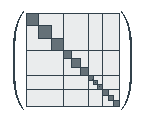
\includegraphics[height = 0.8\linewidth]{../repos/hbp-paper/doc/aistats_talk/logo/hbp_logo_splitting}
  \end{center}
  \vspace{-2ex}
  \captionof{figure}{\textbf{Illustration of sub-blocking.} Here, each diagonal
    block is split into three blocks of equal size.}\label{fig:hbp::subblocking}
}. \Cref{hbp::fig:experiment_fcnn} shows performance curves. In the initial
phase, the BDA can be split into a larger number of sub-blocks without suffering
from a loss in performance. The reduced curvature information is still
sufficient to escape the initial plateau. However, larger blocks have to be
considered in later stages to further reduce the loss efficiently.

The fact that this switch in modularity is necessary is an argument in favor of
the HBP's flexibility to efficiently realize such switches: for this experiment,
the splitting for each block was artificially chosen to illustrate this
flexibility. In principle, the splitting could be decided individually for each
parameter block, and even changed at run time.

\subsubsection{CNN, Matrix-free Exact Curvature Multiplication}

For convolutions, the large number of hidden features prohibits backpropagating
a curvature matrix batch average. Instead, we use exact curvature matrix-vector
products provided within HBP. The CNN possesses sigmoid activations and cannot
be trained by SGD (\Cref{hbp::subfig:experiment_cnn1}). For comparison with
another second-order method, we experiment with a public KFAC
implementation~\citep[see \Cref{hbp::sec:experimentalDetails} for
details]{martens2015optimizing,grosse2016kronecker}.

The matrix-free second-order methods progress fast in the initial stage of the
optimization. However, progress in later phases stagnates. This may be caused by
the limited sophistication of the update rule~\eqref{hbp::equ:linearSystemCG}: if a
small value for $\alpha$ is chosen, the optimizer will perform well in the
beginning (GGN, $\alpha_1$). As the gradients become smaller, and hence more
noisy, the step size limitation is too optimistic, which leads to a slow-down in
optimization progress. A more conservative step size limitation improves the
overall performance at the cost of fewer initial progress (GGN, $\alpha_2$). In
the training phase where damping is ``effective'', our illustrative methods, and
KFAC, exhibit better progress per iteration on the objective than the
first-order competitor Adam, underlining the usefulness of curvature even if
only computed block-wise.

For an impression on performance in terms of run time,
\Cref{hbp::subfig:experiment_cnn2} compares the wall-clock time of one
matrix-free method and the baselines. The HBP-based optimizer can compete with
existing methods and offers potential for further improvements, like
sub-blocking and parallelized CG. Despite the more adaptive nature of
second-order methods, their full power seems to still require adaptive damping,
to account for the quality of the local quadratic approximation and restrict the
update if necessary. The importance of these techniques to properly adapt the
Newton direction has been emphasized in previous works
\citep{martens2010deep,martens2015optimizing, botev2017practical} that aim to
develop fully fletched second-order optimizers. Such adaptation, however, is
beyond the scope of this text.

%%% Local Variables:
%%% mode: latex
%%% TeX-master: "../thesis"
%%% End:


\section{Conclusion}
We have outlined a procedure to compute block-diagonal approximations of
different curvature matrices for feedforward neural networks by a scheme that
can be realized on top of gradient backpropagation. In contrast to other
recently proposed methods, our implementation is aligned with the design of
current machine learning frameworks and can flexibly compute Hessian sub-blocks
to different levels of refinement. Its modular formulation facilitates
closed-form analysis of Hessian diagonal blocks, and unifies previous approaches
\citep{botev2017practical,wei2018bdapch}.

Within our framework we presented two strategies: (i) obtaining exact curvature
matrix-vector products that have not been accessible before by
auto-differentiation (PCH), and (ii) backpropagation of further approximated
matrix representations to save computations during training. As for gradient
backpropagation, the Hessian backpropagation for different operations can be
derived independently of the underlying graph. The extended modules can then be
used as a drop-in replacement for existing modules to construct deep neural
networks. Internally, backprop is extended by an additional Hessian backward
pass through the graph to compute curvature information. It can be performed in
parallel to, and reuse the quantities computed in, gradient backpropagation.

%%% Local Variables:
%%% mode: latex
%%% TeX-master: "../thesis"
%%% End:


\section*{Acknowledgments}
The authors would like to thank Frederik Kunstner, Matthias Werner, Frank
Schneider, and Agustinus Kristiadi for their constructive feedback on the
manuscript, and gratefully acknowledge financial support by the European
Research Council through ERC StG Action 757275 / PANAMA; the DFG Cluster of
Excellence “Machine Learning - New Perspectives for Science”, EXC 2064/1,
project number 390727645; the German Federal Ministry of Education and Research
(BMBF) through the T\"ubingen AI Center (FKZ: 01IS18039A); and funds from the
Ministry of Science, Research and Arts of the State of Baden-W\"urttemberg.
F.\,D.\,is grateful to the International Max Planck Research School for
Intelligent Systems (IMPRS-IS) for support.

%%% Local Variables:
%%% mode: latex
%%% TeX-master: "../thesis"
%%% End:


\setchapterpreamble[u]{\margintoc}
\chapter{BackPACK: Packing More into Backprop}\label{chap:backpack}
\subsubsection{Abstract}

Automatic differentiation frameworks are optimized for exactly one thing:
computing the average mini-batch gradient. Yet, other quantities such as the
variance of the mini-batch gradients or many approximations to the Hessian can,
\emph{in theory}, be computed efficiently, and at the same time as the gradient.
While these quantities are of great interest to researchers and practitioners,
current deep-learning software does not support their automatic calculation.
Manually implementing them is burdensome, inefficient if done na\"ively, and the
resulting code is rarely shared. This hampers progress in deep learning, and
unnecessarily narrows research to focus on gradient descent and its variants; it
also complicates replication studies and comparisons between newly developed
methods that require those quantities, to the point of impossibility. To address
this problem, we introduce \BackPACK, an efficient framework built on top of
\PyTorch, that extends the backpropagation algorithm to extract additional
information from first- and second-order derivatives. Its capabilities are
illustrated by benchmark reports for computing additional quantities on deep
neural networks, and an example application by testing several recent curvature
approximations for optimization.

\marginnote{%
  \begin{center}
    Code and experiments available at the Github repositories
    \href{https://github.com/f-dangel/backpack}{\texttt{f-dangel/backpack}},
    \href{https://github.com/f-dangel/backpack-experiments}{\texttt{f-dangel/backpack-experiments}}
  \end{center}
  \begin{center}
    
\includegraphics[height = 0.8\linewidth]{../repos/backpack-paper/tex/logo/backpack_logo_github.pdf}
  \end{center}
}%

\section{Introduction}
The success of deep learning and the applications it fuels can be traced to the
popularization of automatic differentiation frameworks. Packages like
\TensorFlow~\citep{abadi2016tensorflow}, \Chainer~\citep{tokui2015chainer},
\MXNet~\citep{chen2015mxnet}, and \PyTorch~\citep{paszke2019pytorch} provide
efficient implementations of parallel, GPU-based gradient computations to a wide
range of users, with elegant syntactic sugar.

However, this specialization also has its shortcomings: it assumes the user only
wants to compute gradients or, more precisely, the average of gradients across a
mini-batch of examples. Other quantities can also be computed with AD at a
comparable cost or minimal overhead to the gradient backpropagation pass; for
example, approximate second-order information or the variance of gradients
within the batch. These quantities are valuable to understand the geometry of
deep neural networks, for the identification of free parameters, and to push the
development of more efficient optimization algorithms. But researchers who want
to investigate their use face a chicken-and-egg problem: AD tools required to go
beyond standard gradient methods are not available, but there is no incentive
for their implementation in existing deep-learning software as long as no large
portion of the users need it.

Second-order methods for deep learning have been continuously investigated for
decades \citep[\eg][]{becker1988improving,amari1998natural,bordes2009sgdqn,
  martens2015optimizing}. But still, the standard optimizers used in deep
learning remain some variant of stochastic gradient descent (\SGD); more complex
methods have not found wide-spread, practical use. This is in stark contrast to
domains like convex optimization and generalized linear models, where
second-order methods are the default. There may of course be good scientific
reasons for this difference; maybe second-order methods do not work well in the
(non-convex, stochastic) setting of deep learning. And the computational cost
associated with the high dimensionality of deep models may offset their
benefits. Whether these are the case remains somewhat unclear though, because a
much more direct road-block is that these methods are so complex to implement
that few practitioners ever try them out.

Recent approximate second-order methods such as \KFAC
\citep{martens2015optimizing} show promising results, even on hard deep learning
problems \citep{tsuji2019performance}. Their approach, based on the earlier work
of \citet{schraudolph2002fast}, uses the structure of the network to compute
approximate second-order information in a way that is similar to gradient
backpropagation. This work sparked a new line of research to improve the
second-order approximation \citep{grosse2016kronecker, botev2017practical,
  martens2018kronecker, george2018fast}. However, all of these methods require
low-level applications of automatic differentiation to compute quantities other
than the averaged gradient. It is a daunting task to implement them from
scratch. Unless users spend significant time familiarizing themselves with the
internals of their software tools, the resulting implementation is often
inefficient, which also puts the original usability advantage of those packages
into question. Even motivated researchers trying to develop new methods, who
need not be expert software developers, face this problem. They often end up
with methods that cannot compete in run time, not necessarily because the method
is inherently bad, but because the implementation is not efficient. New methods
are also frequently not compared to their predecessors and competitors because
they are so hard to reproduce. Authors do not want to represent the competition
in an unfair light caused by a bad implementation.

Another example is offered by a recent string of research to adapt to the
\emph{stochasticity} induced by mini-batch sampling. An empirical estimate of
the (marginal) variance of the gradients within the batch has been found to be
theoretically and practically useful for adapting hyperparameters like learning
rates \citep{mahsereci2017probabilistic} and batch sizes
\citep{balles2017coupling}, or regularize first-order optimization
\citep{leroux2007topmoumoute, balles2018dissecting, katharopoulos2018samples}.
To get such a variance estimate, one simply has to square, then sum, the
individual gradients after the backpropagation, but before they are aggregated
to form the average gradient. Doing so should have negligible cost \emph{in
  principle}, but is programmatically challenging in the standard packages.

Members of the community have repeatedly asked for such features\sidenote{See
  \eg the Github issues
  \href{https://github.com/pytorch/pytorch/issues/1407}{\nolinkurl{github.com/pytorch/pytorch/issues/1407}},
  \href{https://github.com/pytorch/pytorch/issues/7786}{\nolinkurl{7786}},
  \href{https://github.com/pytorch/pytorch/issues/8897}{\nolinkurl{8897}} and
  forum discussions
  \href{https://discuss.pytorch.org/t/1433}{\nolinkurl{discuss.pytorch.org/t/1433}},
  \href{https://discuss.pytorch.org/t/8405}{\nolinkurl{8405}},
  \href{https://discuss.pytorch.org/t/15270}{\nolinkurl{15270}},
  \href{https://discuss.pytorch.org/t/17204}{\nolinkurl{17204}},
  \href{https://discuss.pytorch.org/t/19350}{\nolinkurl{19350}},
  \href{https://discuss.pytorch.org/t/24955}{\nolinkurl{24955}}. } %
but the established AD frameworks have yet to address such requests, as their
focus has been---rightly---on improving their technical backbone. Features like
those outlined above are not generally defined for arbitrary functions, but
rather emerge from the specific structure of machine learning applications.
General AD frameworks can not be expected to serve such specialist needs. This
does not mean, however, that it is impossible to efficiently realize such
features within these frameworks: in essence, backpropagation is a technique to
compute multiplications with Jacobians. Methods to extract second-order
information \citep{mizutani2008secondorder} or individual gradients from a
mini-batch \citep{goodfellow2015efficient} have been known to a small group of
specialists; they are just rarely discussed or implemented.

\subsection{Our Contribution}
To address this need for a specialized framework focused on machine learning, we
propose a framework for the implementation of generalized backpropagation to
compute additional quantities. The structure is based on the conceptual work of
\citet{dangel2020modular} for modular backpropagation. This framework can be
built on top of existing graph-based backpropagation modules; we provide an
implementation on top of \PyTorch, coined \BackPACK, available at
~\\[-1.75em]
\begin{center}
  \url{https://f-dangel.github.io/backpack/}.
\end{center}
~\\[-1.75em]
The initial release supports efficient computation of individual gradients from
a mini-batch, their $L_2$ norm, an estimate of the variance, as well as diagonal
and Kronecker factorizations of the generalized Gauss-Newton (\GGN) matrix
(see~\Cref{backpack::tab:features_backpack} for a feature overview). The library
was designed to be minimally verbose to the user, easy to use
(see~\Cref{fig:backpack-code-sample}), and to have low overhead (see
\Cref{backpack::sec:benchmark}). While other researchers are aiming to improve
the flexibility of AD systems \citep{innes2018flux, innes2018zygote,
  bradbury2018jax}, our goal with this package is to provide access to
quantities that are only byproducts of the backpropagation pass, rather than
gradients themselves.

\begin{figure*}[t]
  \centering
  \hfill
  \begin{minipage}[t]{.48\linewidth}
    \textbf{\!Computing the gradient with \pytorchtitle\ldots}\\[1em]
    \footnotesize
    \texttt{%
      X, y~~~~~= load\_mnist\_data()\\
      model~~~~= Linear(784, 10)\\
      lossfunc~= CrossEntropyLoss()\\
      ~\\
      loss~~~~~= lossfunc(model(X), y)\\
      ~\\
      loss.backward()\\
      ~\\
      for param in model.parameters():~\\
      \null\hspace{2.5em}print(param.grad)
    }
  \end{minipage}\hspace{-0.5em}\vline\hfill
  \begin{minipage}[t]{.48\linewidth}
    \textbf{\!\ldots and the variance with \backpacktitle}\\[1em]
    \footnotesize
    \texttt{%
      X, y~~~~~= load\_mnist\_data()\\
      model~~~~= \textbf{\color{maincolor} extend(}Linear(784, 10)\textbf{\color{maincolor})}\\
      lossfunc~= \textbf{\color{maincolor} extend(}CrossEntropyLoss()\textbf{\color{maincolor})}\\
      ~\\
      loss~~~~~= lossfunc(model(X), y)\\
      \textbf{\color{maincolor} with backpack(Variance()):}\\
      \null\hspace{2.5em}loss.backward()\\
      ~\\
      for param in model.parameters():~\\
      \null\hspace{2.5em}print(param.grad)\\
      \textbf{\color{maincolor} \null\hspace{2.5em}print(param.var)}
    }
  \end{minipage}
  \vspace{-2ex}
  \captionof{lstlisting}{ \textbf{\BackPACK integrates with \PyTorch to
      seamlessly extract more information from the backward pass.} Instead of
    the variance (or alongside it, in the same pass), \BackPACK can compute
    individual gradients in the mini-batch, their $L_2$ norm and
    2\textsuperscript{nd} moment. It can also compute curvature approximations
    like diagonal or Kronecker factorizations of the \GGN such as \KFAC, \KFLR
    \& \KFRA. }
  \label{fig:backpack-code-sample}
\end{figure*}

%%% Local Variables:
%%% mode: latex
%%% TeX-master: "../../thesis"
%%% End:


To illustrate the capabilities of \BackPACK, we use it to implement
preconditioned gradient descent optimizers with diagonal approximations of the
\GGN and recent Kronecker factorizations \KFAC \citep{martens2015optimizing},
\KFLR, and \KFRA \citep{botev2017practical}. Our results show that the curvature
approximations based on Monte Carlo (\MC) estimates of the \GGN, the approach
used by \KFAC, give similar progress per iteration to their more accurate
counterparts, but being much cheaper to compute. While the naïve update rule we
implement does not surpass first-order baselines such as \SGD with momentum and
Adam \citep{kingma2015adam}, its implementation with various curvature
approximations is made straightforward.

%%% Local Variables:
%%% mode: latex
%%% TeX-master: "../thesis"
%%% End:


\section{Theory \& Implementation}\label{backpack::sec:theory-and-implementation}
We will distinguish between quantities that can be computed from information
already present during a traditional backward pass (which we suggestively call
\emph{first-order extensions}), and quantities that need additional information
(termed \emph{second-order extensions}). The former group contains additional
statistics such as the variance of the gradients within the mini-batch or the
$L_2$ norm of the gradient for each sample. Those can be computed with
minimal overhead during the backprop pass. The latter class contains
approximations of second-order information, like the diagonal or Kronecker
factorization of the generalized Gauss-Newton (\GGN) matrix, which require the
propagation of additional information through the graph. We will present those
two classes separately:

\begin{figure*}[!h]
  \centering
  \begin{minipage}[t]{0.495\linewidth}
    \begin{center}
      \textbf{First-order extensions}\\
      Extract more from the standard backward pass.~\\[-.75em]
      \begin{itemize}
      \item Individual gradients from a mini-batch
      \item $L_2$ norm of the individual gradients
      \item Diagonal covariance and 2\textsuperscript{nd} moment
      \end{itemize}
    \end{center}
  \end{minipage}
  \hfill
  \begin{minipage}[t]{0.495\linewidth}
    \begin{center}
      \textbf{Second-order extensions}\\
      Propagate new information along the graph.~\\[-.75em]
      \begin{itemize}
      \item Diagonal of the \GGN%
        and the Hessian
      \item \KFAC%
        \citep{martens2015optimizing}
      \item \KFRA%
        and \KFLR%
        \citep{botev2017practical}
      \end{itemize}
    \end{center}
  \end{minipage}
\end{figure*}

These quantities are only defined, or reasonable to compute, for a subset of
models: the concept of individual gradients for each sample in a mini-batch or
the estimate of the variance requires the loss for each sample to be
independent. While such functions are common in machine learning, not all neural
networks fit into this category. \Eg if the network uses batch normalization
\citep{ioffe2015batch}, the individual gradients in a mini-batch are correlated.
Then, the variance is not meaningful anymore, and computing the individual
contribution of a sample to the mini-batch gradient or the \GGN%
becomes prohibitive. For those reasons, and to limit the scope of the project
for version 1.0, \BackPACK%
currently restricts the type of models it accepts. The supported models are
traditional feedforward networks that can be expressed as a \emph{sequence of
  modules}, for example a sequence of convolutional, pooling, linear and
activation layers. Recurrent networks like \LSTM%
\!\!s \citep{hochreither1997lstm} or residual networks \citep{he2016deep} are
not yet supported, but the framework can be extended to cover them\sidenote{%
  \BackPACK has been continuously developed since the initial release.
  Noteworthy added features include:
  \begin{itemize}
  \item New extensions: per-sample Hessian/GGN diagonal (version 1.3),
    matrix-free multiplication with block-diagonal curvature matrices from
    \Cref{chap:hbp} (version 1.2), and \ggn low-rank factors (versions 1.4, 1.5),
    see \Cref{chap:vivit}.
  \item Broader support of modules and hyperparameters, especially basic support
    for residual and recurrent networks (version 1.4).
  \end{itemize}
}.

We assume a sequential model $f_{\vtheta}: \times \sX \rightarrow \sF$
and a dataset of $N$ samples $(\vx_n, \vy_n) \in \sX \times \sY$ with
$n=1,\dots, N$. The model maps each sample $\vx_n$ to a prediction
$f_{\vtheta}(\vx_n)$ using some parameters $\vtheta \in \sTheta$. The
predictions are evaluated with a loss function $\ell : \sF \times \sY
\rightarrow \R$, for example the softmax cross-entropy
(\Cref{eq:background::supervisedLearning}), which compares them to the ground
truth $\vy_n$. This leads to the objective function $\mathcal{L}: \sTheta
\rightarrow \R$,
\begin{equation}
  \label{backpack::eq:objective}
  \Loss(\vtheta)
  =
  \frac{1}{N} \sum_{n=1}^N \ell(f_{\vtheta}(\vx_n), \vy_n)\equationPunctuation{.}
\end{equation}
As a shorthand, we will use $\ell_n(\vtheta) = \ell(f_{\vtheta}(\vx_n), \vy_n)$
for the loss and $\vf_n(\vtheta) = f_{\vtheta}(\vx_n)$ for the model output of
individual samples. Our goal is to provide more information about the
derivatives of ${\{\ell_n(\vtheta)\}}_{n=1}^{N}$ \wrt the parameters
$\vtheta$ of the model $f_{\vtheta}$.

\subsection{Primer on Backpropagation}

ML libraries with integrated automatic differentiation use the
modular structure of $\vf_n(\vtheta)$ to compute derivatives
(see~\cite{baydin2018automatic} for an overview). If $f_{\vtheta}$ is a sequence
of $L$ transformations, it can be expressed as
\begin{equation}
  \vf_n(\vtheta)
  =
  \left(
    f^{(L)}_{\vtheta^{(L)}} \circ \ldots \circ f^{(1)}_{\vtheta^{(1)}}
  \right)(\vx_n)\equationPunctuation{,}
\end{equation}
where $f^{(l)}_{\vtheta^{(l)}}$ is the $l$th transformation with parameters
$\vtheta^{(l)}$, such that $\vtheta = ( \vtheta^{(1)\top}, \ldots, \vtheta^{(L)\top} )^{\top}$.
The loss function can also be seen as another transformation, appended to the
network. Let $\vz_n^{(l-1)}, \vz_n^{(l)}$ denote the input and output of the
operation $f^{(l)}_{\vtheta^{(l)}}$ for sample $n$, such that $\vz_n^{(0)}$ is
the original data and $\vz_n^{(1)}, \ldots, \vz_n^{(L)}$
represent the transformed output of each layer, leading to the computation graph\\[-.5em]
\[
  \textstyle \vz_n^{(0)}
  \stackrel{f^{(1)}_{\vtheta^{(1)}}(\vz_n^{(0)})}{\verylongrightarrow}
  \vz_n^{(1)}
  \stackrel{f^{(2)}_{\vtheta^{(2)}}(\vz_n^{(1)})}{\verylongrightarrow} \ldots
  \stackrel{f^{(L)}_{\vtheta^{(L)}}(\vz_n^{(L-1)})}{\verylongrightarrow}
  \vz_n^{(L)} \stackrel{\ell(\vz_n^{(L)}, \vy_n)}{\verylongrightarrow}
  \ell_n(\vtheta)\equationPunctuation{.}
\]
To compute the gradient of $\ell_n$ \wrt $\vtheta^{(l)}$, one unrolls the chain rule,
\begin{equation}
  \begin{split}
    \grad{\vtheta^{(l)}} \ell_n(\vtheta)
    &=
      {\left(\jac_{\vtheta^{(l)}}
      \vz_n^{(l)}\right)}^\top
      {\left(\jac_{\vz_n^{(l)}} \vz_n^{(l+1)}\right)}^\top
      \cdots
      {\left(\jac_{\vz_n^{(L-1)}} \vz_n^{(L)}\right)}^\top
      \grad{\vz_n^{(L)}}\ell_n(\vtheta)
    \\
    &=
      {\left(\jac_{\vtheta^{(l)}} \vz_n^{(l)}\right)}^\top
      \grad{\vz^{(l)}}\ell_n(\vtheta)\equationPunctuation{,}
  \end{split}\label{backpack::eq:backprop_gradient}
\end{equation}
where $\jac_{\va} \vb$ is the Jacobian of $\vb$ \wrt $\va$, ${[\jac_{\va}
  \vb]}_{i,j} = \partial {[\vb]}_i / \partial {[\va]}_j$ (see
\Cref{def:background::JacobianVectorVector}). A similar expression exists for
the module inputs $\vz_n^{(l-1)}$: $ \grad{\vz_n^{(l-1)}}\ell_n(\vtheta) =
(\jac_{\vz_n^{(l-1)}} \vz_n^{(l)})^\top \grad{\vz_n^{(l)}}\ell_n(\vtheta). $
This recursive structure makes it possible to extract the gradient by
propagating the gradient of the loss. In the backpropagation algorithm, a module
$l$ receives the loss gradient \wrt its output,
$\grad{\vz_n^{(l)}}\ell_n(\vtheta)$. It then extracts the gradient with respect
to its parameters and inputs, $\grad{\vtheta^{(l)}}\ell_n(\vtheta)$ and
$\grad{\vz_n^{(l-1)}}\ell_n(\vtheta)$, according to
\Cref{backpack::eq:backprop_gradient}. The gradient \wrt its input is sent
further down the graph. This process, illustrated in
\Cref{backpack::fig:backprop-gradient}, is repeated for each transformation
until all gradients are computed. To implement backpropagation, each module only
needs to know how to multiply with its Jacobians.

\begin{figure}[!t]
  \centering
  \tikzexternalenable%
  \begin{tikzpicture}
  \definecolor{lightGray}{HTML}{b3b3b3}
  \pgfmathsetmacro{\figureWidthPt}{\linewidth}

  \node (im) [inner sep=0pt] {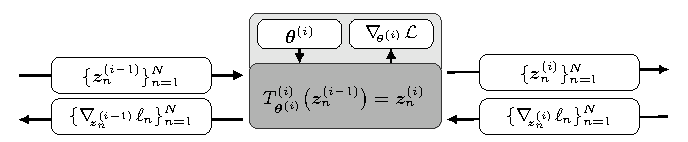
\includegraphics[width=\figureWidthPt pt]{../repos/backpack-paper/tex/paper/figs/backprop-modules/vanilla_backprop.pdf}};

  \newcommand{\relativeCoordinate}[2]{($(im.south west)!#1!(im.south east)+(im.south west)!#2!(im.north west)-(im.south west)$)}

  % bottom left
  \node [rectangle, fill=white, draw=none, inner sep=0pt, minimum height =
  0.04*\figureWidthPt pt, minimum width = 0.18*\figureWidthPt pt, anchor=center]
  at \relativeCoordinate{0.19}{0.18} {$\{ \grad{\vz_n^{(l-1)}}\ell_n \}_n$};

  % top left
  \node [rectangle, fill=white, draw=none, inner sep=0pt, minimum height =
  0.04*\figureWidthPt pt, minimum width = 0.18*\figureWidthPt pt, anchor=center]
  at \relativeCoordinate{0.19}{0.47} {$\{ \vz_n^{(l-1)}\}_n$};

  % bottom right
  \node [rectangle, fill=white, draw=none, inner sep=0pt, minimum height =
  0.04*\figureWidthPt pt, minimum width = 0.18*\figureWidthPt pt, anchor=center]
  at \relativeCoordinate{0.81}{0.18} {$\{ \grad{\vz_n^{(l)}}\ell_n \}_n$};

  % top right
  \node [rectangle, fill=white, draw=none, inner sep=0pt, minimum height =
  0.04*\figureWidthPt pt, minimum width = 0.18*\figureWidthPt pt, anchor=center]
  at \relativeCoordinate{0.81}{0.49} {$\{ \vz_n^{(l)}\}_n$};

  % center left
  \node [rectangle, fill=white, draw=none, inner sep=0pt, minimum height =
  0.035*\figureWidthPt pt, minimum width = 0.1*\figureWidthPt pt, anchor=center]
  at \relativeCoordinate{0.435}{0.76} {$\vtheta^{(l)}$};

  % center right
  \node [rectangle, fill=white, draw=none, inner sep=0pt, minimum height =
  0.035*\figureWidthPt pt, minimum width = 0.1*\figureWidthPt pt, anchor=center]
  at \relativeCoordinate{0.5685}{0.76} {$\grad{\vtheta^{(l)}}\gL$};

  % module
  \node [rectangle, fill=lightGray, draw=none, inner sep=0pt, minimum height =
  0.07*\figureWidthPt pt, minimum width = 0.25*\figureWidthPt pt, anchor=center]
  at \relativeCoordinate{0.5}{0.33} {$f_{\vtheta^{(l)}}^{(l)}$};
\end{tikzpicture}
%%% Local Variables:
%%% mode: latex
%%% TeX-master: "../../thesis"
%%% End:

  \tikzexternaldisable%
  \caption{\textbf{Schematic representation of the standard backpropagation
      pass} for module $l$ with $N$
    samples.}\label{backpack::fig:backprop-gradient}
\end{figure}

For second-order quantities, we rely on the work of
\citet{mizutani2008secondorder} and \citet{dangel2020modular}, who showed that a
scheme similar to \Cref{backpack::eq:backprop_gradient} exists for the
\emph{block diagonal} of the Hessian. A block \wrt the parameters of
a module, $\gradsquared{\vtheta^{(l)}}\ell_n(\vtheta)$, can be obtained by the
recursion
\begin{equation}
  \begin{split}
    \gradsquared{\vtheta^{(l)}}\ell_n(\vtheta)
    &=
    {\left(\jac_{\vtheta^{(l)}} \vz_n^{(l)}\right)}^\top
    \gradsquared{\vz_n^{(l)}}\ell_n(\vtheta)
    \left(\jac_{\vtheta^{(l)}} \vz_n^{(l)}\right)
    \\
    &\phantom{=}\
    + \sum_j
    \left(\gradsquared{\vtheta^{(l)}} {\left[\vz_n^{(l)}\right]}_j\right)
    {\left[ \grad{\vz_n^{(l)}}\ell_n(\vtheta) \right]}_j\equationPunctuation{.}
  \end{split}
  \label{backpack::eq:backprop_hessian}
\end{equation}
A similar relation holds for the module's output Hessian
$\gradsquared{\vz_n^{(l)}} \ell_n(\vtheta)$.

Both backpropagations of
\Cref{backpack::eq:backprop_gradient,backpack::eq:backprop_hessian} hinge on the
multiplication by Jacobians to both vectors and matrices. However, the design of
AD limits the application of Jacobians to vectors only. This prohibits the
exploitation of vectorization in the matrix case, which is needed for
second-order information. The lacking flexibility of Jacobians is one motivation
for our work. Since all quantities needed to compute statistics of the
derivatives are already computed during the backward pass, another motivation is
to provide access to them at minor overhead.

\subsection{First-order Extensions}
As the principal first-order extension, consider computing the \emph{per-sample}
gradients in a batch of size $N$. These individual gradients are implicitly
computed during a traditional backward pass because the batch gradient is their
sum, but they are not directly accessible. The naïve way to compute $N$
individual gradients is to do $N$ separate forward and backward passes, This
(inefficiently) replaces every matrix-matrix multiplication by $N$ matrix-vector
multiplications. \BackPACK batches computations to obtain large efficiency
gains, as illustrated by
\Cref{backpack::fig:bench-individual-gradients}\sidenote{%
  The latest developments in ML libraries have lead to more efficient
  alternatives than the for-loop. \pytorch 1.11.0 (released on March 10, 2022)
  introduced an \inlinecode{is\_grads\_batched} argument in the API of
  the
  \href{https://pytorch.org/docs/1.11/generated/torch.autograd.grad.html}{\inlinecode{grad}}
  function of
  its \href{https://pytorch.org/docs/1.11/autograd.html}{\inlinecode{autograd}}
  library, which allows to compute multiple VJPs in parallel. This reflects the
  importance of the feature.}.

\begin{figure}
  \centering
  \pgfkeys{/pgfplots/BackPACKBenchBarplot/.style={
    width=1.02\linewidth,
    height=0.5\linewidth,
    grid=major,
    grid style = {dashed},
    every axis plot/.append style={line width = 1.5pt},
    tick pos = left,
    xtick align = outside,
    ytick align = inside,
    xmajorticks = true,
    ymajorticks = true,
    ylabel near ticks,
    xlabel near ticks,
    xticklabel style = {font = \footnotesize},
    xlabel style = {font = \footnotesize},
    axis line style = {black},
    yticklabel style = {font = \footnotesize},
    ylabel style = {font = \footnotesize},
    title style = {font = \footnotesize, inner ysep = 0ex},
    grid = major,
    grid style = {dashed},
    legend cell align = left,
    legend style = {
      fill opacity = 0.7,
      text opacity = 1,
      font = \footnotesize,
      legend columns = 4,
      legend cell align={left},
      legend image post style={opacity = 1, yscale = 1.1, line width=-1pt},
      column sep=0.25cm,
    },
  }
}

%%% Local Variables:
%%% mode: latex
%%% TeX-master: "../../thesis"
%%% End:

  \pgfkeys{/pgfplots/zmystyle/.style={
      BackPACKBenchBarplot
    }
  }
  \tikzexternalenable%
  % This file was created by tikzplotlib v0.9.7.
\begin{tikzpicture}

\definecolor{color0}{rgb}{0.211764705882353,0.294117647058824,0.603921568627451}
\definecolor{color1}{rgb}{0.431372549019608,0.650980392156863,0.803921568627451}
\definecolor{color2}{rgb}{0.76078431372549,0.894117647058824,0.937254901960784}

\begin{axis}[
legend cell align={left},
legend style={fill opacity=0.8, draw opacity=1, text opacity=1, draw=white!80!black},
tick align=outside,
tick pos=left,
title={Batch gradients},
x grid style={white!69.0196078431373!black},
xmin=-0.5125, xmax=2.5125,
xtick style={color=black},
xtick={0,1,2},
xticklabels={For-loop,BackPACK,Gradient
(Ref.)},
y grid style={white!69.0196078431373!black},
ylabel={Time [ms]},
ymin=0, ymax=715.401721642411,
ytick style={color=black},
zmystyle
]
\draw[draw=none,fill=white!20!black] (axis cs:1.625,0) rectangle (axis cs:1.875,22.247069500736);
\draw[draw=none,fill=color0] (axis cs:-0.375,0) rectangle (axis cs:-0.125,190.67248400097);
\addlegendimage{ybar,ybar legend,draw=none,fill=color0};
\addlegendentry{Batch size 64}

\draw[draw=none,fill=color0] (axis cs:0.625,0) rectangle (axis cs:0.875,30.771913996432);
\draw[draw=none,fill=white!40!black] (axis cs:1.875,0) rectangle (axis cs:2.125,40.6486490028328);
\draw[draw=none,fill=color1] (axis cs:-0.125,0) rectangle (axis cs:0.125,367.899422002665);
\addlegendimage{ybar,ybar legend,draw=none,fill=color1};
\addlegendentry{                 128}

\draw[draw=none,fill=color1] (axis cs:0.875,0) rectangle (axis cs:1.125,57.7847249951446);
\draw[draw=none,fill=color2] (axis cs:0.125,0) rectangle (axis cs:0.375,681.334972992772);
\addlegendimage{ybar,ybar legend,draw=none,fill=color2};
\addlegendentry{                 256}

\draw[draw=none,fill=color2] (axis cs:1.125,0) rectangle (axis cs:1.375,96.5649990030215);
\draw[draw=none,fill=white!60!black] (axis cs:2.125,0) rectangle (axis cs:2.375,79.2037880019052);
\addplot [semithick, white!20!black, opacity=0.4, forget plot]
table {%
-0.5125 22.247069500736
2.5125 22.247069500736
};
\addplot [semithick, white!40!black, opacity=0.4, forget plot]
table {%
-0.5125 40.6486490028329
2.5125 40.6486490028329
};
\addplot [semithick, white!60!black, opacity=0.4, forget plot]
table {%
-0.5125 79.2037880019052
2.5125 79.2037880019052
};
\end{axis}

\end{tikzpicture}

  \tikzexternaldisable%
  \caption{\textbf{Computing individual gradients in a batch using a for-loop
      (\ie one individual forward and backward pass per sample) or using
      vectorized operations with \BackPACK.} The plot shows computation time,
    comparing to a traditional gradient computation, on the \CIFARTENNET%
    network (see \Cref{backpack::sec:experiments}) for the \CIFARTEN%
    dataset \citep{schneider2019deepobs}.
  }\label{backpack::fig:bench-individual-gradients}
\end{figure}

As the quantities necessary to compute the individual gradients are already
propagated through the computation graph, we can reuse them by inserting code in
the standard backward pass. With access to this information, before it is
cleared for memory efficiency, \BackPACK%
computes the Jacobian-multiplications
for each sample
\begin{equation}
  {\left\{
      \grad{\vtheta^{(l)}} \ell_n(\vtheta)
    \right\}}_{n=1}^N
  =
  {\left\{
      {\left(\jac_{\vtheta^{(l)}} \vz^{(l)}_n\right)}^\top \grad{\vz_n^{(l)}} \ell_n(\vtheta)
    \right\}}_{n=1}^N\equationPunctuation{,}
\end{equation}
without summing the result---see \Cref{backpack::fig:first-order-extraction} for
a schematic representation. This duplicates some of the computation performed by
the backpropagation, as the Jacobian is applied twice (once by \PyTorch%
and \BackPACK%
with and without summation over the samples, respectively). However, the
associated overhead is small compared to the for-loop approach: the major
computational cost arises from the propagation of information required for each
layer, rather than the formation of the gradient \emph{within} each layer.

This scheme for individual gradient computation is the basis for all first-order
extensions. In this direct form, however, it is expensive in memory: if the
model is $D$-dimensional, storing $\gO(ND)$ elements is prohibitive for large
batches. For the variance, 2\textsuperscript{nd} moment and $L_2$ norm,
\BackPACK%
takes advantage of the Jacobian's structure to directly compute them without
forming the individual gradient, reducing memory overhead. See
\Cref{backpack::app:first-order-extensions} for details.

\begin{figure}[!t]
  \centering
  \tikzexternalenable%
  \begin{tikzpicture}
  \definecolor{lightBlue}{HTML}{d1e5f0}
  \definecolor{lightGray}{HTML}{b3b3b3}
  \pgfmathsetmacro{\figureWidthPt}{\linewidth}

  \node (im) [inner sep=0pt] {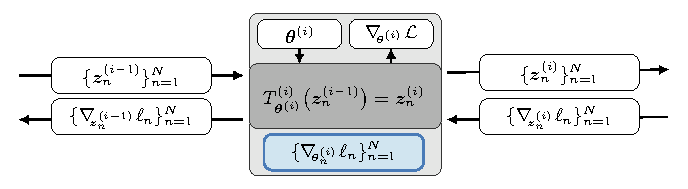
\includegraphics[width=\figureWidthPt pt]{../repos/backpack-paper/tex/paper/figs/backprop-modules/indiv_grad.pdf}};

  \newcommand{\relativeCoordinate}[2]{($(im.south west)!#1!(im.south east)+(im.south west)!#2!(im.north west)-(im.south west)$)}

  % bottom left
  \node [rectangle, fill=white, draw=none, inner sep=0pt, minimum height =
  0.04*\figureWidthPt pt, minimum width = 0.18*\figureWidthPt pt, anchor=center]
  at \relativeCoordinate{0.19}{0.385} {$\{ \grad{\vz_n^{(l-1)}}\ell_n \}_n$};

  % top left
  \node [rectangle, fill=white, draw=none, inner sep=0pt, minimum height =
  0.04*\figureWidthPt pt, minimum width = 0.18*\figureWidthPt pt, anchor=center]
  at \relativeCoordinate{0.19}{0.6} {$\{ \vz_n^{(l-1)}\}_n$};

  % bottom right
  \node [rectangle, fill=white, draw=none, inner sep=0pt, minimum height =
  0.04*\figureWidthPt pt, minimum width = 0.18*\figureWidthPt pt, anchor=center]
  at \relativeCoordinate{0.81}{0.385} {$\{ \grad{\vz_n^{(l)}}\ell_n \}_n$};

  % top right
  \node [rectangle, fill=white, draw=none, inner sep=0pt, minimum height =
  0.04*\figureWidthPt pt, minimum width = 0.18*\figureWidthPt pt, anchor=center]
  at \relativeCoordinate{0.81}{0.615} {$\{ \vz_n^{(l)}\}_n$};

  % center left
  \node [rectangle, fill=white, draw=none, inner sep=0pt, minimum height =
  0.03*\figureWidthPt pt, minimum width = 0.1*\figureWidthPt pt, anchor=center]
  at \relativeCoordinate{0.435}{0.82} {$\vtheta^{(l)}$};

  % center right
  \node [rectangle, fill=white, draw=none, inner sep=0pt, minimum height =
  0.03*\figureWidthPt pt, minimum width = 0.1*\figureWidthPt pt, anchor=center]
  at \relativeCoordinate{0.5685}{0.82} {$\grad{\vtheta^{(l)}}\gL$};

  % module
  \node [rectangle, fill=lightGray, draw=none, inner sep=0pt, minimum height =
  0.05*\figureWidthPt pt, minimum width = 0.25*\figureWidthPt pt, anchor=center]
  at \relativeCoordinate{0.5}{0.49} {$f_{\vtheta^{(l)}}^{(l)}$};

  % center bottom
  \node [rectangle, fill=lightBlue, draw=none, inner sep=0pt, minimum height =
  0.04*\figureWidthPt pt, minimum width = 0.2*\figureWidthPt pt, anchor=center]
  at \relativeCoordinate{0.5}{0.195} {$\{ \grad{\vtheta^{(l)}} \ell_n\}_n$};
\end{tikzpicture}
%%% Local Variables:
%%% mode: latex
%%% TeX-master: "../../thesis"
%%% End:

  \tikzexternaldisable%
  \caption{\textbf{Schematic representation of the individual gradients'
      extraction in addition to the standard backward pass} at the $l$th module
      for $N$ samples.}\label{backpack::fig:first-order-extraction}
\end{figure}

\subsection{Second-order Extensions}\label{backpack::sec:backpack-second-order}
Second-order extensions require propagation of more information through the
graph. %
\marginnote[*-20]{
  \begin{example}[\textbf{Symmetric decomposition of the softmax cross-entropy loss
    Hessian~\cite{papyan2019measurements}}]\label{ex:backpack::symmetricDecompositionCE}
  Consider the softmax cross-entropy loss
  (\Cref{eq:background::softmaxCrossEntropyLoss}) Hessian from Table
  \Cref{hbp::table:backpropEquations}. Its symmetric decomposition $\mS \in
  \sR^{C\times C}$ is
    \begin{align}
      \label{eq:backpack::sqrtCrossEntropyLoss}
      \begin{split}
        \mS
        &=
          \left(
          \mI - \vp\,\vone^{\top}
          \right)
          \diag\left( \sqrt{\vp} \right)
        \\
        &=
          \diag\left( \sqrt{\vp} \right)
          -
          \vp \sqrt{\vp}^{\top}\,,
      \end{split}
    \end{align}
    where $\sqrt{\vp(\vf)} = {\vp(\vf)}^{\odot \nicefrac{1}{2}}$. It satisfies
    $\gradsquared{\vf}\ell(\vf, \vy) = \mS \mS^{\top}$,
    \begin{align*}
      \mS \mS^{\top}
      &=
        \left[
        \diag\left( \sqrt{\vp} \right)
        -
        \vp \sqrt{\vp}^{\top}\,
        \right]
      \\
      &\phantom{= \ }
        \left[
        \diag\left( \sqrt{\vp} \right)
        -
        \sqrt{\vp} \vp^{\top}\,
        \right]
      \\
      &=
        \diag\left( \vp \right)
        - 2 \vp \vp^{\top}
        + \vp \sqrt{\vp}^{\top}
        \sqrt{\vp} \vp^{\top}
      \\
      &=
        \diag\left( \vp \right)
        - \vp \vp^{\top}\,,
    \end{align*}
    using that $\vp$'s elements sum to one, \ie $\sqrt{\vp}^{\top}\sqrt{\vp} =
    1$. This is the expression from \Cref{hbp::table:backpropEquations}.
  \end{example}
}%
As an example, we will focus on the \GGN matrix
\citep{schraudolph2002fast}. It is guaranteed to be PSD and is a reasonable
approximation of the Hessian near the minimum, which motivates its use in
approximate second-order methods. For popular loss functions, it coincides with
the Fisher information matrix used in natural gradient methods
\citep{amari1998natural}; for a more in depth discussion of the equivalence, see
\Cref{sec:background::naturalGradientDescent} and the reviews of
\citet{martens2014new} and \citet{kunstner2019limitations}. For an objective
function that can be written as the composition of a loss function $\ell$ and a
model $f_{\vtheta}$, such as \Cref{backpack::eq:objective}, the \GGN%
of $\nicefrac{1}{N} \sum_n \ell(f_{\vtheta}(\vx_n), \vy_n)$ is
\begin{equation}
  \label{backpack::eq:main-ggn}
  \mG(\vtheta) =
  \frac{1}{N} \sum_n
  {\left(\jac_\vtheta \vf_n \right)}^\top
  \gradsquared{\vf_n} \ell(\vf_n, \vy_n) \:
  \left(\jac_\vtheta \vf_n\right)\equationPunctuation{.}
\end{equation}
\marginnote[*-10]{%
  \begin{example}[\textbf{\mc approximation of the softmax-cross entropy loss
    Hessian}]\label{ex:backpack::symmetricMCDecompositionCE} Consider the softmax
  cross-entropy loss (\Cref{eq:background::softmaxCrossEntropyLoss}) Hessian
  from \Cref{hbp::table:backpropEquations}. An \mc approximation of the
  symmetric decomposition (\Cref{eq:backpack::sqrtCrossEntropyLoss}) is
  constructed by the vectors
    \begin{align}
      \label{equ:backpack::sqrtMCVectorsCrossEntropyLoss}
      \vstilde = \vytilde(c) - \vp(\vf)
    \end{align}
    with $\vytilde(c) = \onehot(c)$ and $c$ drawn from a categorical
    distribution implied by the softmax-probabilities, $c \sim \Cat(c;
    \vp(\vf))$. The random vector $\vytilde$ satisfies $\E_{c}\left[ \vytilde
    \right] = \vp(\vf)$ and $\E_{c}\left[ \vytilde \vytilde^{\top} \right] =
    \diag[\vp(\vf)]$. With these properties, we can show
    $\E_{\vstilde}\left[\vstilde\vstilde^{\top}\right] = \gradsquared{\vf}\ell$,
    \ie%
    the expected outer product of
    \Cref{equ:backpack::sqrtMCVectorsCrossEntropyLoss} is the Hessian,
    \begin{align*}
      \E_{\vstilde} \left[\vstilde \vstilde^{\top}\right]
      &=
        \E_{c}[ \vytilde \vytilde^{\top} ]
        - \E_{c}[ \vytilde]  \vp^{\top}
      \\
      &\phantom{= \,}
        -  \vp \E_{c}[\vytilde^{\top} ]
        + \vp \vp^{\top}
      % \\
      % &=
      %   \diag(\vp) - 2 \vp \vp^{\top} + \vp\vp^{\top}
      \\
      &=
        \diag(\vp) - \vp \vp^{\top}\,.
    \end{align*}
    Instead of using the $C \times C$ matrix square root $\mS$, we can draw $M <
    C$ samples $c_1, \dots, c_M$ and stack their $\vstilde$-vectors into a
    smaller $C \times M $ matrix
    \begin{align}
      \mStilde
      =
      \frac{1}{\sqrt{M}}
      \begin{pmatrix}
        \vstilde(c_1)\  \dots\  \vstilde(c_M)
      \end{pmatrix}
    \end{align}
    that approximates \Cref{eq:backpack::sqrtCrossEntropyLoss},
    \begin{align*}
      \mStilde \mStilde^{\top}
      &=
        \frac{1}{M}
        \sum_{i=1}^{M}
        \vstilde(c_i)
        {\vstilde(c_i)}^{\top}
      \\
      &\approx \E_{\vstilde}\left[ \vstilde \vstilde^{\top}\right]
        = \mS \mS^{\top}\,,
    \end{align*}
    using less memory. From the connection between Fisher and Hessian,
    \Cref{equ:backpack::sqrtMCVectorsCrossEntropyLoss} are `would-be gradients'
    under targets sampled from the model's likelihood, \ie%
    $\vstilde^{\top} = \jac_{\vf}\ell(\vf, \vytilde)$ with $\vytilde \sim
    q(\giventhat{\cdot}{\vf})$ and the Jacobian from
    \Cref{tab:background::Jacobians}.
  \end{example}
}%
The full matrix is too large to compute and store. Current approaches focus on
its diagonal blocks, where each block corresponds to a layer in the network.
Every block itself is further approximated, for example using a Kronecker
factorization. The approach used by \BackPACK%
for their computation is a refinement of the \emph{Hessian Backpropagation
  equations} of \citet{dangel2020modular}. It relies on two insights: firstly,
the computational bottleneck in the \ggn's computation is the multiplication
with the Jacobian of the network, $\jac_\vtheta \vf_n$, while the network output
Hessian is easy to compute for most popular loss functions. Secondly, it is not
necessary to compute and store each of the $N$ $D \times D$ matrices for a
network with $D$ parameters, as \Cref{backpack::eq:main-ggn} is a quadratic
expression. Given a symmetric factorization $\mS_n$ of the Hessian,
$\mS_n\mS_n^\top = \gradsquared{\vf_n} \ell(\vf_n, \vy_n)$ (\eg
\Cref{ex:backpack::symmetricDecompositionCE}), it is sufficient to compute
${(\jac_\vtheta \vf_n)}^\top \mS_n$ and square the result. A network output is
typically small compared to its inner layers; networks on \CIFARHUN%
need $C=100$ class outputs but could use convolutional layers with more than
100,000 parameters.

The factorization leads to a $D \times C$ matrix, which makes it possible to
efficiently compute \GGN%
block diagonals. Also, the computation is very similar to that of a gradient,
which computes ${(\jac_\vtheta \vf_n)}^\top \grad{\vf_n} \ell_n$. A module
$f^{(l)}_{\vtheta^{(l)}}$ receives the symmetric factorization of the \GGN%
\wrt its output, $\vz^{(l)}_n$, and multiplies it with the Jacobians
\wrt the parameters $\vtheta^{(l)}$ and inputs $\vz^{(l-1)}_n$ to
produce a symmetric factorization of the \GGN%
\wrt the parameters and inputs, as shown in
\Cref{backpack::fig:second-order-pass}.

\begin{figure}[!t]
  \centering
  \tikzexternalenable%
  \begin{tikzpicture}
  \definecolor{lightBlue}{HTML}{d1e5f0}
  \definecolor{lightGray}{HTML}{b3b3b3}
  \pgfmathsetmacro{\figureWidthPt}{\linewidth}

  \node (im) [inner sep=0pt] {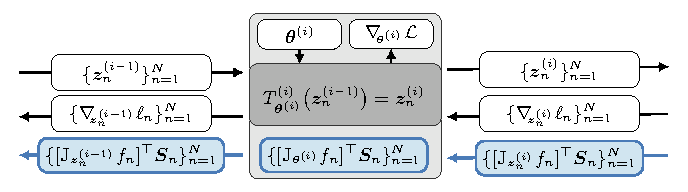
\includegraphics[width=\figureWidthPt pt]{../repos/backpack-paper/tex/paper/figs/backprop-modules/second_order.pdf}};

  \newcommand{\relativeCoordinate}[2]{($(im.south west)!#1!(im.south east)+(im.south west)!#2!(im.north west)-(im.south west)$)}

  % bottom left
  \node [rectangle, fill=lightBlue, draw=none, inner sep=0pt, minimum height =
  0.04*\figureWidthPt pt, minimum width = 0.245*\figureWidthPt pt, anchor=center]
  at \relativeCoordinate{0.19}{0.195} {$\{ {(\jac_{\vz_n^{(l-1)}} \vf_n)}^{\top} \mS_n \}_n$};

  % center left
  \node [rectangle, fill=white, draw=none, inner sep=0pt, minimum height =
  0.04*\figureWidthPt pt, minimum width = 0.18*\figureWidthPt pt, anchor=center]
  at \relativeCoordinate{0.19}{0.41} {$\{ \grad{\vz_n^{(l-1)}}\ell_n \}_n$};

  % top left
  \node [rectangle, fill=white, draw=none, inner sep=0pt, minimum height =
  0.04*\figureWidthPt pt, minimum width = 0.18*\figureWidthPt pt, anchor=center]
  at \relativeCoordinate{0.19}{0.625} {$\{ \vz_n^{(l-1)}\}_n$};

  % bottom right
  \node [rectangle, fill=lightBlue, draw=none, inner sep=0pt, minimum height =
  0.04*\figureWidthPt pt, minimum width = 0.225*\figureWidthPt pt, anchor=center]
  at \relativeCoordinate{0.814}{0.18} {$\{ {(\jac_{\vz_n^{(l)}} \vf_n)}^{\top} \mS_n \}_n$};

  % center right
  \node [rectangle, fill=white, draw=none, inner sep=0pt, minimum height =
  0.04*\figureWidthPt pt, minimum width = 0.18*\figureWidthPt pt, anchor=center]
  at \relativeCoordinate{0.81}{0.41} {$\{ \grad{\vz_n^{(l)}}\ell_n \}_n$};

  % top right
  \node [rectangle, fill=white, draw=none, inner sep=0pt, minimum height =
  0.04*\figureWidthPt pt, minimum width = 0.18*\figureWidthPt pt, anchor=center]
  at \relativeCoordinate{0.81}{0.64} {$\{ \vz_n^{(l)}\}_n$};

  % center left
  \node [rectangle, fill=white, draw=none, inner sep=0pt, minimum height =
  0.03*\figureWidthPt pt, minimum width = 0.1*\figureWidthPt pt, anchor=center]
  at \relativeCoordinate{0.435}{0.82} {$\vtheta^{(l)}$};

  % center right
  \node [rectangle, fill=white, draw=none, inner sep=0pt, minimum height =
  0.03*\figureWidthPt pt, minimum width = 0.1*\figureWidthPt pt, anchor=center]
  at \relativeCoordinate{0.5685}{0.82} {$\grad{\vtheta^{(l)}}\gL$};

  % module
  \node [rectangle, fill=lightGray, draw=none, inner sep=0pt, minimum height =
  0.05*\figureWidthPt pt, minimum width = 0.25*\figureWidthPt pt, anchor=center]
  at \relativeCoordinate{0.5}{0.49} {$\vf_{\vtheta^{(l)}}^{(l)}$};

  % center bottom
  \node [rectangle, fill=lightBlue, draw=none, inner sep=0pt, minimum height =
  0.04*\figureWidthPt pt, minimum width = 0.22*\figureWidthPt pt, anchor=center]
  at \relativeCoordinate{0.5}{0.195} {$\{ {(\jac_{\vtheta^{(l)}} \vf_n)}^{\top} \mS_n \}_n$};
\end{tikzpicture}
%%% Local Variables:
%%% mode: latex
%%% TeX-master: "../../thesis"
%%% End:

  \tikzexternaldisable%
  \caption{\textbf{Schematic of the additional backward pass} to compute a
    symmetric factorization of the \GGN,
    \begin{align*}
      \mG(\vtheta) = \frac{1}{N} \sum_n {\left(\jac_{\vtheta} \vf_n\right)}^\top \mS_n \mS_n^\top
      \left(\jac_{\vtheta} \vf_n\right)
    \end{align*}
    alongside the gradient at the $l$th module, for $N$ samples.
  }\label{backpack::fig:second-order-pass}
\end{figure}

This propagation serves as the basis of the second-order extensions. If the full
symmetric factorization is not wanted, for memory reasons, it is possible to
extract more specific information such as the diagonal. If $\mB$ is the
symmetric factorization for a \GGN%
block, the diagonal can be computed as $[\diag(\mB\mB^\top)]_{i} =
{[\mB\mB^\top]}_{i,i} = \sum_j {[\mB]}_{i,j}^2$.

This framework can be used to extract the main Kronecker factorizations of the
\GGN, \KFAC%
and \KFLR, which we extend to convolution using the approach of
\citet{grosse2016kronecker}. The important difference between the two methods is
the initial matrix factorization $\mS_n$. Using a full symmetric factorization
of the initial Hessian, $\mS_n\mS_n^\top = \gradsquared{\vf_n}\ell_n$, yields
the \KFLR%
approximation. \KFAC%
uses an \MC approximation by sampling a vector $\vs_n$ such that
$\mathbb{E}_{\vs_n}[\vs_n\vs_n^\top] = \gradsquared{\vf_n} \ell_n$ (see
\Cref{ex:backpack::symmetricMCDecompositionCE}). \KFLR%
is therefore more precise but more expensive than \KFAC, especially for networks
with high-dimensional outputs, which is reflected in our benchmark on \CIFARHUN%
in \Cref{backpack::sec:benchmark}. The technical details on how Kronecker
factors are extracted and information is propagated for second-order \BackPACK%
extensions are documented in \Cref{backpack::app:second-order-extensions}.

%%% Local Variables:
%%% mode: latex
%%% TeX-master: "../thesis"
%%% End:


\section{Evaluation \& Benchmarks}\label{backpack::sec:benchmark}
We benchmark the overhead of \BackPACK %
on \CIFARTEN and \CIFARHUN, using the \CIFARTENNET network and the \ALLCNNC
network of \citet{springenberg2015striving} provided by \DeepOBS
\citep{schneider2019deepobs}\sidenote{\CIFARTENNET is a sequence of three
  convolutions and three dense linear layers with 895,210 parameters. \ALLCNNC
  is a sequence of nine convolutions with 1,387,108 parameters.}.
\Cref{backpack::fig:benchmark-all} shows the results.

For first-order extensions, the computation of individual gradients from a
mini-batch adds noticeable overhead due to the additional memory requirements to
store them. But more specific quantities such as the $L_2$ norm,
2\textsuperscript{nd} moment and variance can be extracted efficiently.
Regarding second-order extensions, the \ggn computation can be expensive for
nets with large outputs like \CIFAR{100}, regardless of the approximation being
diagonal of Kronecker-factored. Thankfully, the \MC approximation used by \KFAC,
which we also implement for a diagonal approximation, can be computed at minimal
overhead---much less than two backward passes. This last point is encouraging,
as our optimization experiment in \Cref{backpack::sec:experiments} suggest that
this approximation is reasonably accurate.

%%% Local Variables:
%%% mode: latex
%%% TeX-master: "../thesis"
%%% End:


\section{Experiments}\label{backpack::sec:experiments}
To illustrate the utility of \BackPACK, we implement preconditioned gradient
descent optimizers using diagonal and Kronecker approximations of the \GGN. To
our knowledge, and despite their apparent simplicity, results using diagonal
approximations or the naïve damping update rule we chose have not been reported
in publications so far. However, this section is not meant to introduce a
bona-fide new optimizer. Our goal is to show that \BackPACK can enable research
of this kind. The update rule we implement uses a curvature matrix
$\mC(\vtheta_t^{(l)})$, which could be a diagonal or Kronecker factorization of
the \GGN blocks, and a damping parameter $\lambda$ to precondition the gradient:
\begin{equation}
  \label{backpack::eq:update_rule}
  \vtheta_{t+1}^{(l)}
  =
  \vtheta_t^{(l)} - \eta \left(\mC(\vtheta_t^{(l)}) + \lambda \mI\right)^{-1}
  \grad{\vtheta_t^{(l)}}\Loss(\vtheta_t^{(l)})\equationPunctuation{,}
  \qquad l = 1,\dots, L\equationPunctuation{.}
\end{equation}
We run the update rule with the following approximations of the generalized
Gauss-Newton: the exact diagonal (\DiagGGN) and an \MC estimate (\DiagGGNMC),
and the Kronecker factorizations \KFAC \citep{martens2015optimizing}, \KFLR and
\KFRA\sidenote{ \KFRA was not originally designed for convolutions; we extend it
  using the Kronecker factorization of \citet{grosse2016kronecker}. While it can
  be computed for small networks on \MNIST, which we report in
  \Cref{backpack::app:additional-results}, the approximate backward pass of
  \KFRA does not seem to scale to large convolution layers. }
\citep{botev2017practical}.%
The inversion required by the update rule is straightforward for the diagonal
curvature. For the Kronecker-factored quantities, we use the approximation
introduced by \cite{martens2015optimizing} (see
\Cref{backpack::app:update_rule_details}).

\begin{figure*}[!t]
  \centering
  \pgfkeys{/pgfplots/BackPACKBenchBarplot/.style={
    width=1.02\linewidth,
    height=0.5\linewidth,
    grid=major,
    grid style = {dashed},
    every axis plot/.append style={line width = 1.5pt},
    tick pos = left,
    xtick align = outside,
    ytick align = inside,
    xmajorticks = true,
    ymajorticks = true,
    ylabel near ticks,
    xlabel near ticks,
    xticklabel style = {font = \footnotesize},
    xlabel style = {font = \footnotesize},
    axis line style = {black},
    yticklabel style = {font = \footnotesize},
    ylabel style = {font = \footnotesize},
    title style = {font = \footnotesize, inner ysep = 0ex},
    grid = major,
    grid style = {dashed},
    legend cell align = left,
    legend style = {
      fill opacity = 0.7,
      text opacity = 1,
      font = \footnotesize,
      legend columns = 4,
      legend cell align={left},
      legend image post style={opacity = 1, yscale = 1.1, line width=-1pt},
      column sep=0.25cm,
    },
  }
}

%%% Local Variables:
%%% mode: latex
%%% TeX-master: "../../thesis"
%%% End:

  \begin{subfigure}[t]{1.0\linewidth}
    \centering
    \caption{\threecthreed, \cifarten}\label{backpack::subfig:benchmark-all1}
    \vspace{-1ex}
    \pgfkeys{/pgfplots/zmystyle/.style={
        BackPACKBenchBarplot,
        height = 0.35\linewidth,
        title = \empty,
      }
    }
    \tikzexternalenable
    % This file was created by tikzplotlib v0.9.7.
\begin{tikzpicture}

\definecolor{color0}{rgb}{0.211764705882353,0.294117647058824,0.603921568627451}
\definecolor{color1}{rgb}{0.431372549019608,0.650980392156863,0.803921568627451}
\definecolor{color2}{rgb}{0.76078431372549,0.894117647058824,0.937254901960784}

\begin{axis}[
legend cell align={left},
legend columns=4,
legend style={fill opacity=0.8, draw opacity=1, text opacity=1, at={(0.03,0.97)}, anchor=north west, draw=white!80!black},
tick align=outside,
tick pos=left,
title={3C3D on CIFAR10},
x grid style={white!69.0196078431373!black},
xmin=-0.5, xmax=7.5,
xtick style={color=black},
xtick={0,1,2,3,4,5,6,7},
xticklabels={
Grad (ref.),2nd Moment,
Batch L2,DiagGGN-MC,
KFAC,Indiv. Grad,
KFLR,DiagGGN},
y grid style={white!69.0196078431373!black},
ylabel={Time [ms]},
ymin=0, ymax=50,
ytick style={color=black},
zmystyle
]
\draw[draw=none,fill=white!20!black] (axis cs:-0.375,0) rectangle (axis cs:-0.125,15.0664545000154);
\draw[draw=none,fill=color0] (axis cs:0.625,0) rectangle (axis cs:0.875,14.395405000073);
\addlegendimage{ybar,ybar legend,draw=none,fill=color0};
\addlegendentry{Batch = 32}

\draw[draw=none,fill=color0] (axis cs:1.625,0) rectangle (axis cs:1.875,15.2878979999969);
\draw[draw=none,fill=color0] (axis cs:2.625,0) rectangle (axis cs:2.875,19.3677970000863);
\draw[draw=none,fill=color0] (axis cs:3.625,0) rectangle (axis cs:3.875,16.8086539999877);
\draw[draw=none,fill=color0] (axis cs:4.625,0) rectangle (axis cs:4.875,15.2265290000742);
\draw[draw=none,fill=color0] (axis cs:5.625,0) rectangle (axis cs:5.875,21.8555310000283);
\draw[draw=none,fill=color0] (axis cs:6.625,0) rectangle (axis cs:6.875,22.4338249999505);
\draw[draw=none,fill=white!40!black] (axis cs:-0.125,0) rectangle (axis cs:0.125,20.5737690000092);
\draw[draw=none,fill=color1] (axis cs:0.875,0) rectangle (axis cs:1.125,20.6966069999908);
\addlegendimage{ybar,ybar legend,draw=none,fill=color1};
\addlegendentry{48}

\draw[draw=none,fill=color1] (axis cs:1.875,0) rectangle (axis cs:2.125,20.9739174999868);
\draw[draw=none,fill=color1] (axis cs:2.875,0) rectangle (axis cs:3.125,25.4147299999659);
\draw[draw=none,fill=color1] (axis cs:3.875,0) rectangle (axis cs:4.125,22.383585);
\draw[draw=none,fill=color1] (axis cs:4.875,0) rectangle (axis cs:5.125,20.8398080000052);
\draw[draw=none,fill=color1] (axis cs:5.875,0) rectangle (axis cs:6.125,30.4188420000173);
\draw[draw=none,fill=color1] (axis cs:6.875,0) rectangle (axis cs:7.125,33.1303219999199);
\draw[draw=none,fill=white!60!black] (axis cs:0.125,0) rectangle (axis cs:0.375,26.3089910000645);
\draw[draw=none,fill=color2] (axis cs:1.125,0) rectangle (axis cs:1.375,26.2560775000225);
\addlegendimage{ybar,ybar legend,draw=none,fill=color2};
\addlegendentry{64}

\draw[draw=none,fill=color2] (axis cs:2.125,0) rectangle (axis cs:2.375,28.7451689999898);
\draw[draw=none,fill=color2] (axis cs:3.125,0) rectangle (axis cs:3.375,32.0420350000177);
\draw[draw=none,fill=color2] (axis cs:4.125,0) rectangle (axis cs:4.375,28.0495179999889);
\draw[draw=none,fill=color2] (axis cs:5.125,0) rectangle (axis cs:5.375,30.8939720000581);
\draw[draw=none,fill=color2] (axis cs:6.125,0) rectangle (axis cs:6.375,37.0278835000022);
\draw[draw=none,fill=color2] (axis cs:7.125,0) rectangle (axis cs:7.375,47.5826415000711);
\addplot [semithick, white!20!black, opacity=0.4, forget plot]
table {%
-0.5 15.0664545000154
7.5 15.0664545000154
};
\addplot [semithick, white!40!black, opacity=0.4, forget plot]
table {%
-0.5 20.5737690000092
7.5 20.5737690000092
};
\addplot [semithick, white!60!black, opacity=0.4, forget plot]
table {%
-0.5 26.3089910000645
7.5 26.3089910000645
};
\end{axis}

\end{tikzpicture}

    \tikzexternaldisable
  \end{subfigure}
  \begin{subfigure}[t]{1.0\linewidth}
    \centering
    \caption{\allcnnc, \cifarhun}\label{backpack::subfig:benchmark-all2}
    \vspace{-1ex}
    \pgfkeys{/pgfplots/zmystyle/.style={
        BackPACKBenchBarplot,
        height = 0.35\linewidth,
        ylabel = {Time [ms]},
        title = \empty,
      }
    }
    \tikzexternalenable
    \hspace{-1ex}% This file was created by tikzplotlib v0.9.7.
\begin{tikzpicture}

\definecolor{color0}{rgb}{0.211764705882353,0.294117647058824,0.603921568627451}
\definecolor{color1}{rgb}{0.431372549019608,0.650980392156863,0.803921568627451}
\definecolor{color2}{rgb}{0.76078431372549,0.894117647058824,0.937254901960784}

\begin{axis}[
legend cell align={left},
legend columns=4,
legend style={fill opacity=0.8, draw opacity=1, text opacity=1, at={(0.03,0.97)}, anchor=north west, draw=white!80!black},
tick align=outside,
tick pos=left,
title={All-CNN-C on CIFAR100},
x grid style={white!69.0196078431373!black},
xmin=-0.5, xmax=5.5,
xtick style={color=black},
xtick={0,1,2,3,4,5},
xticklabels={
Grad (ref.),2nd Moment,
Batch L2,DiagGGN-MC,
KFAC,Indiv. Grad},
y grid style={white!69.0196078431373!black},
ymin=0, ymax=113.550937500011,
ytick style={color=black},
zmystyle
]
\draw[draw=none,fill=white!20!black] (axis cs:-0.375,0) rectangle (axis cs:-0.125,17.0513680000113);
\draw[draw=none,fill=color0] (axis cs:0.625,0) rectangle (axis cs:0.875,23.2273660000146);
\addlegendimage{ybar,ybar legend,draw=none,fill=color0};
\addlegendentry{Batch = 32}

\draw[draw=none,fill=color0] (axis cs:1.625,0) rectangle (axis cs:1.875,29.9791224999808);
\draw[draw=none,fill=color0] (axis cs:2.625,0) rectangle (axis cs:2.875,27.1620119999625);
\draw[draw=none,fill=color0] (axis cs:3.625,0) rectangle (axis cs:3.875,38.6299799999961);
\draw[draw=none,fill=color0] (axis cs:4.625,0) rectangle (axis cs:4.875,55.4445244999897);
\draw[draw=none,fill=white!40!black] (axis cs:-0.125,0) rectangle (axis cs:0.125,23.4135965000064);
\draw[draw=none,fill=color1] (axis cs:0.875,0) rectangle (axis cs:1.125,32.411140000022);
\addlegendimage{ybar,ybar legend,draw=none,fill=color1};
\addlegendentry{48}

\draw[draw=none,fill=color1] (axis cs:1.875,0) rectangle (axis cs:2.125,39.3030079999335);
\draw[draw=none,fill=color1] (axis cs:2.875,0) rectangle (axis cs:3.125,38.0351860000019);
\draw[draw=none,fill=color1] (axis cs:3.875,0) rectangle (axis cs:4.125,53.98943900002);
\draw[draw=none,fill=color1] (axis cs:4.875,0) rectangle (axis cs:5.125,81.7799224999476);
\draw[draw=none,fill=white!60!black] (axis cs:0.125,0) rectangle (axis cs:0.375,30.1599859999442);
\draw[draw=none,fill=color2] (axis cs:1.125,0) rectangle (axis cs:1.375,41.9460425000011);
\addlegendimage{ybar,ybar legend,draw=none,fill=color2};
\addlegendentry{64}

\draw[draw=none,fill=color2] (axis cs:2.125,0) rectangle (axis cs:2.375,49.1684415000009);
\draw[draw=none,fill=color2] (axis cs:3.125,0) rectangle (axis cs:3.375,48.6743639999077);
\draw[draw=none,fill=color2] (axis cs:4.125,0) rectangle (axis cs:4.375,69.9318230000472);
\draw[draw=none,fill=color2] (axis cs:5.125,0) rectangle (axis cs:5.375,108.143750000011);
\addplot [semithick, white!20!black, opacity=0.4, forget plot]
table {%
-0.5 17.0513680000113
5.5 17.0513680000113
};
\addplot [semithick, white!40!black, opacity=0.4, forget plot]
table {%
-0.5 23.4135965000064
5.5 23.4135965000064
};
\addplot [semithick, white!60!black, opacity=0.4, forget plot]
table {%
-0.5 30.1599859999442
5.5 30.1599859999442
};
\end{axis}

\end{tikzpicture}

    \tikzexternaldisable
  \end{subfigure}
  \caption{ \textbf{Overhead benchmark for computing the gradient \emph{and}
      first- or second-order extensions on real networks, compared to just the
      gradient.} Most quantities add little overhead. \KFLR and \DiagGGN
    propagate 100$\times$ more information than \KFAC and \DiagGGNMC on
    \CIFAR{100} and are two orders of magnitude slower. We report benchmarks on
    those, and the Hessian's diagonal, in \Cref{backpack::app:benchmark}. }
  \label{backpack::fig:benchmark-all}
\end{figure*}


\begin{figure*}[!t]
  \centering
  \begin{subfigure}[t]{1.0\linewidth}
    \centering
    \caption{}\label{backpack::subfig:cifar1}
    \vspace{-5.5ex}
    \begin{center}\textbf{\footnotesize \CIFARTEN : \CIFARTENNET}\end{center}
    \tikzexternalenable
    \plotDifferentCurvatures{cifar10}{3c3d}{const}{final}{valid}{accuracies}
    \tikzexternaldisable
  \end{subfigure}
  \vspace{-2ex}
  \begin{subfigure}[t]{1.0\linewidth}
    \centering
    \caption{}\label{backpack::subfig:cifar2}
    \vspace{-5.5ex}
    \begin{center}\textbf{\footnotesize \CIFARHUN : \ALLCNNC}\end{center}
    \tikzexternalenable
    \plotDifferentCurvatures{cifar100}{allcnnc}{const}{final}{valid}{accuracies}
    \tikzexternaldisable
  \end{subfigure}
  \caption{\textbf{Median performance with shaded quartiles of the \DeepOBS
      benchmark} for \subfigref{backpack::subfig:cifar1} \CIFARTENNET (895,210
    parameters) on \CIFARTEN and \subfigref{backpack::subfig:cifar1} \ALLCNNC
    (1,387,108 parameters) on \CIFARHUN. Solid lines show \DeepOBS' baselines of
    momentum \SGD and Adam.}
  \label{backpack::fig:cifar}
\end{figure*}

These curvature estimates are tested for the training of deep neural networks by
running the corresponding optimizers on the main test problems of the
benchmarking suite \DeepOBS\sidenote{%
  \href{https://deepobs.github.io/}{\texttt{deepobs.github.io}}. We cannot run
  \BackPACK on all test problems in this benchmark due to the limitations
  outlined in \Cref{backpack::sec:theory-and-implementation}. Despite this
  limitation, we still run on models spanning a representative range of image
  classification problems. } \citep{schneider2019deepobs}. We use the setup
(batch size, number of training epochs) of \DeepOBS' baselines, and tune the
learning rate $\eta$ and damping parameter $\lambda$ with a grid search for
each optimizer (details in \Cref{backpack::app:grid-search}). The best
hyperparameter settings is chosen according to the final accuracy on a
validation set. We report the median and quartiles of the performance for ten
random seeds.

\Cref{backpack::subfig:cifar1} shows the results for the \CIFARTENNET network
trained on \CIFAR{10}. The optimizers that leverage Kronecker-factored curvature
approximations beat the baseline performance in terms of per-iteration progress
on the training loss, training and test accuracy. Using the same
hyperparameters, there is little difference between \KFAC and \KFLR, or \DiagGGN
and \DiagGGNMC. Given that the quantities based on \MC-sampling are considerably
cheaper, this experiment suggests it being an important technique to reduce
the computational burden of curvature proxies.

\Cref{backpack::subfig:cifar2} shows benchmarks for the \ALLCNNC network trained
on \CIFAR{100}. Due to the high-dimensional output, the curvatures using a full
matrix propagation rather than an \MC sample cannot be run on this problem due
to memory issues. Both \DiagGGNMC and \KFAC can compete with the baselines in
terms of progress per iteration. As the update rule we implemented is simplistic
on purpose, this is promising for future applications of second-order methods
that can more efficiently use the additional information given by curvature
approximations.

%%% Local Variables:
%%% mode: latex
%%% TeX-master: "../thesis"
%%% End:


\section{Conclusion}
\begin{table}[!t]
  \centering
  \caption{\textbf{Overview of the features supported in the first release of
      \BackPACK.}}\label{backpack::tab:features_backpack}
  \begin{footnotesize}
    \begin{tabular}{llll}
      \toprule
      &
        \textbf{Feature}
      &
        \textbf{Details}
      \\
      \midrule
      &
        Individual gradients
      &
        $\frac{1}{N} \grad{\vtheta^{(l)}}\ell_n(\vtheta), \quad n=1,\dots, N$
      &
      \\
      &
        Batch variance
      &
        $\frac{1}{N}\sum_{n=1}^{N}
        \left[\grad{\vtheta^{(l)}}\ell_n(\vtheta)\right]_j^2 -
        \left[\grad{\vtheta^{(l)}}\gL (\vtheta) \right]_j^2$
      &
      \\
      &
        2\textsuperscript{nd} moment
      &
        $\frac{1}{N} \sum_{n=1}^{N}\left[\grad{\vtheta^{(l)}}\ell_n(\vtheta)\right]_j^2, \quad j = 1,\dots,d^{(l)}$.
      &
      \\
      &
        Indiv. gradient $L_2$ norm
      &
        $\left\lVert \frac{1}{N}  \grad{\vtheta^{(l)}}\ell_n(\vtheta) \right\rVert_2^2,\quad n=1,\dots,N$
      &
      \\
      &
        \DiagGGN
      &
        $\diag\left(\mG(\vtheta^{(l)})\right)$
      &
      \\
      &
        \DiagGGNMC
      &
        $\diag\left(\mGtilde(\vtheta^{(l)})\right)$
      &
      \\
      &
        Hessian diagonal
      &
        $\diag\left(\gradsquared{\vtheta}\gL(\vtheta) \right)$
      &
      \\
      &
        \KFAC
      &
        $\mGtilde^{(l)}(\vtheta^{(l)}) \approx \mA^{(l)} \otimes \mB^{(l)}_\text{\KFAC}$
      &
      \\
      &
        \KFLR
      &
        $\mG^{(l)}(\vtheta^{(l)}) \approx \mA^{(l)} \otimes \mB^{(l)}_\text{\KFLR}$
      &
      \\
      &
        \KFRA
      &
        $\mG^{(l)}(\vtheta^{(l)}) \approx \mA^{(l)} \otimes \mB^{(l)}_\text{\KFRA}$
      &
      \\
      \bottomrule
    \end{tabular}
  \end{footnotesize}
\end{table}

Machine learning's coming-of-age has been accompanied, and in part driven, by a
maturing of the software ecosystem. This has drastically simplified the lives of
developers and researchers alike, but has also crystallized parts of the
algorithmic landscape. This has dampened research in cutting-edge areas that are
far from mature, like second-order optimization for deep neural networks. To
ensure that good ideas can bear fruit, researchers must be able to compute new
quantities without an overwhelming software development burden. To support
research and development in optimization for deep learning, we have introduced
\BackPACK, an efficient implementation in \PyTorch of recent conceptual advances
and extensions to backpropagation (\Cref{backpack::tab:features_backpack} lists
all features). \BackPACK enriches the syntax of AD packages to offer additional
observables to optimizers beyond the batch-averaged gradient. Our experiments
demonstrate that \BackPACK's implementation offers drastic efficiency gains over
the kind of na\"ive implementation within reach of the typical researcher. As a
demonstrative example, we ``invented'' a few optimization routines that, without
\BackPACK, would require demanding implementation work and can now be tested
with ease. We hope that studies like this allow \BackPACK to help mature the ML
software ecosystem further.

\section*{Acknowledgments}

We would like to thank Aaron Bahde, Ludwig Bald, and Frank Schneider for their help
with \DeepOBS and Lukas Balles, Simon Bartels, Filip de Roos, Tim Fischer,
Nicolas Kr\"amer, Agustinus Kristiadi, Frank Schneider, Jonathan Wenger, and
Matthias Werner for constructive feedback.


The authors gratefully acknowledge financial support by the European Research Council through ERC StG Action 757275 / PANAMA; the DFG Cluster of Excellence “Machine Learning - New Perspectives for Science”, EXC 2064/1, project number 390727645; the German Federal Ministry of Education and Research (BMBF) through the T\"ubingen AI Center (FKZ: 01IS18039A); and funds from the Ministry of Science, Research and Arts of the State of Baden-W\"urttemberg. F.\ D.\ is grateful to the International Max Planck Research School for Intelligent Systems (IMPRS-IS) for support.

%%% Local Variables:
%%% mode: latex
%%% TeX-master: "../thesis"
%%% End:


%%% Local Variables:
%%% mode: latex
%%% TeX-master: "../thesis"
%%% End:


\setchapterpreamble[u]{\margintoc}
\chapter{Cockpit: A Practical Debugging Tool for the Training of Deep
  Neural Networks}\label{chap:cockpit}
\subsubsection{Abstract}

When engineers train deep learning models, they are very much ``flying blind''.
Commonly used methods for real-time training diagnostics, such as monitoring the
train/test loss, are limited. Assessing a net's training process solely through
these performance indicators is akin to debugging software without access to
internal states through a debugger. To address this, we present \cockpit, a
collection of instruments that enable a closer look into the inner workings of a
learning machine, and a more informative and meaningful status report for
practitioners. It facilitates the identification of learning phases and failure
modes, like ill-chosen hyperparameters. The instruments leverage novel
higher-order information about the gradient distribution and curvature, which
has only recently become efficiently accessible. We believe that such a
debugging tool, which we open-source for \pytorch, is valuable in
troubleshooting the training process. By revealing new insights, it also more
generally contributes to explainability and interpretability of deep nets.

\marginnote{%
  \begin{center}
    Code and experiments available at the Github repositories
    \href{https://github.com/f-dangel/cockpit}{\texttt{f-dangel/cockpit}},
    \href{https://github.com/f-dangel/cockpit-experiments}{\texttt{f-dangel/cockpit-experiments}}
  \end{center}
  \begin{center}
    
\includegraphics[height = 0.8\linewidth]{../repos/cockpit/docs/source/_static/LogoSquare}
  \end{center}
}

\section{Introduction \& Motivation}\label{cockpit::sec:intro}
Deep learning represents a new programming paradigm: instead of deterministic
programs, users design models and ``simply'' train them with data. In this
metaphor, deep learning is a meta-programming form, where \emph{coding} is
replaced by \emph{training}. Here, we ponder the question how we can provide
more insight into this process by building a \emph{debugger} specifically
designed for deep learning.

Debuggers are crucial for traditional software development. When things fail,
they provide access to the internal workings of the code, allowing a look ``into
the box''. This is much more efficient than re-running the program with
different inputs. And yet, deep learning is arguably closer to the latter. If
the attempt to train a deep net fails, a machine learning engineer faces various
options: should they change the training hyperparameters (how?); the optimizer
(to which one?); the model (how?); or just re-run with a different seed? Machine
learning toolboxes provide scant help to guide these decisions.

Of course, traditional debuggers can be applied to deep learning. They will give
access to every single weight of a neural net, or the individual pixels of its
training data. But this rarely yields insights towards successful training.
Extracting meaningful information requires a statistical approach and
distillation of the bewildering complexity into a manageable summary. Tools like
\tensorboard \citep{abadi2016tensorflow} or \wandb \citep{biewald2020experiment} were built in part
to streamline this visualization. Yet, the quantities that are widely monitored
(mainly train/test loss \& accuracy), provide only scant explanation for
relative differences between multiple training runs, because \emph{they do not
  show the network's internal state}. \Cref{cockpit::fig:LINE} illustrates how such
established learning curves can describe the \emph{current} state of the model
-- whether it is performing well or not -- while failing to inform about
training state and dynamics. They tell the user \emph{that} things are going
well or badly, but not \emph{why}. The situation is similar to flying a plane by
sight, without instruments to provide feedback. It is not surprising, then, that
achieving state-of-the-art performance in deep learning requires expert
intuition, or plain trial \& error.

\begin{figure*}[!t]
  \centering
  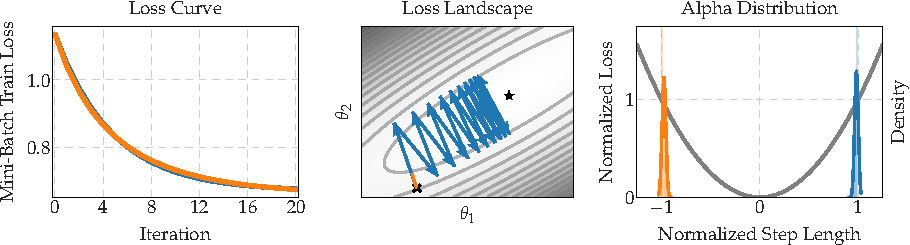
\includegraphics{../repos/cockpit-paper/fig/02_LINE/output/LINE_thesis-wide}
  \caption{\textbf{Illustrative example: learning curves do not tell the whole
      story}. Two different optimization runs
    (\textcolor{sns_orange}{\textbf{---}}/\textcolor{sns_blue}{\textbf{---}})
    can lead to virtually the same loss curve (\textit{left}). However, the
    actual optimization trajectories (\textit{middle}), exhibit vastly different
    behaviors. In practice, the trajectories are intractably large and cannot be
    visualized directly. Recommendable actions for both scenarios
    (\textcolor{sns_orange}{increase}/\textcolor{sns_blue}{decrease} the
    learning rate) cannot be inferred from the loss curve. The
    $\alpha$-distribution, one \cockpit instrument (\textit{right}), not only
    clearly distinguishes the two scenarios, but also allows for taking
    decisions how the learning rate should be adapted. See
    \Cref{cockpit::sec:alpha_exp} for further details.}\label{cockpit::fig:LINE}
\end{figure*}

\begin{figure*}[!t]
  \centering
  % trim={<left> <lower> <right> <upper>}, clip
  \Cshadowbox{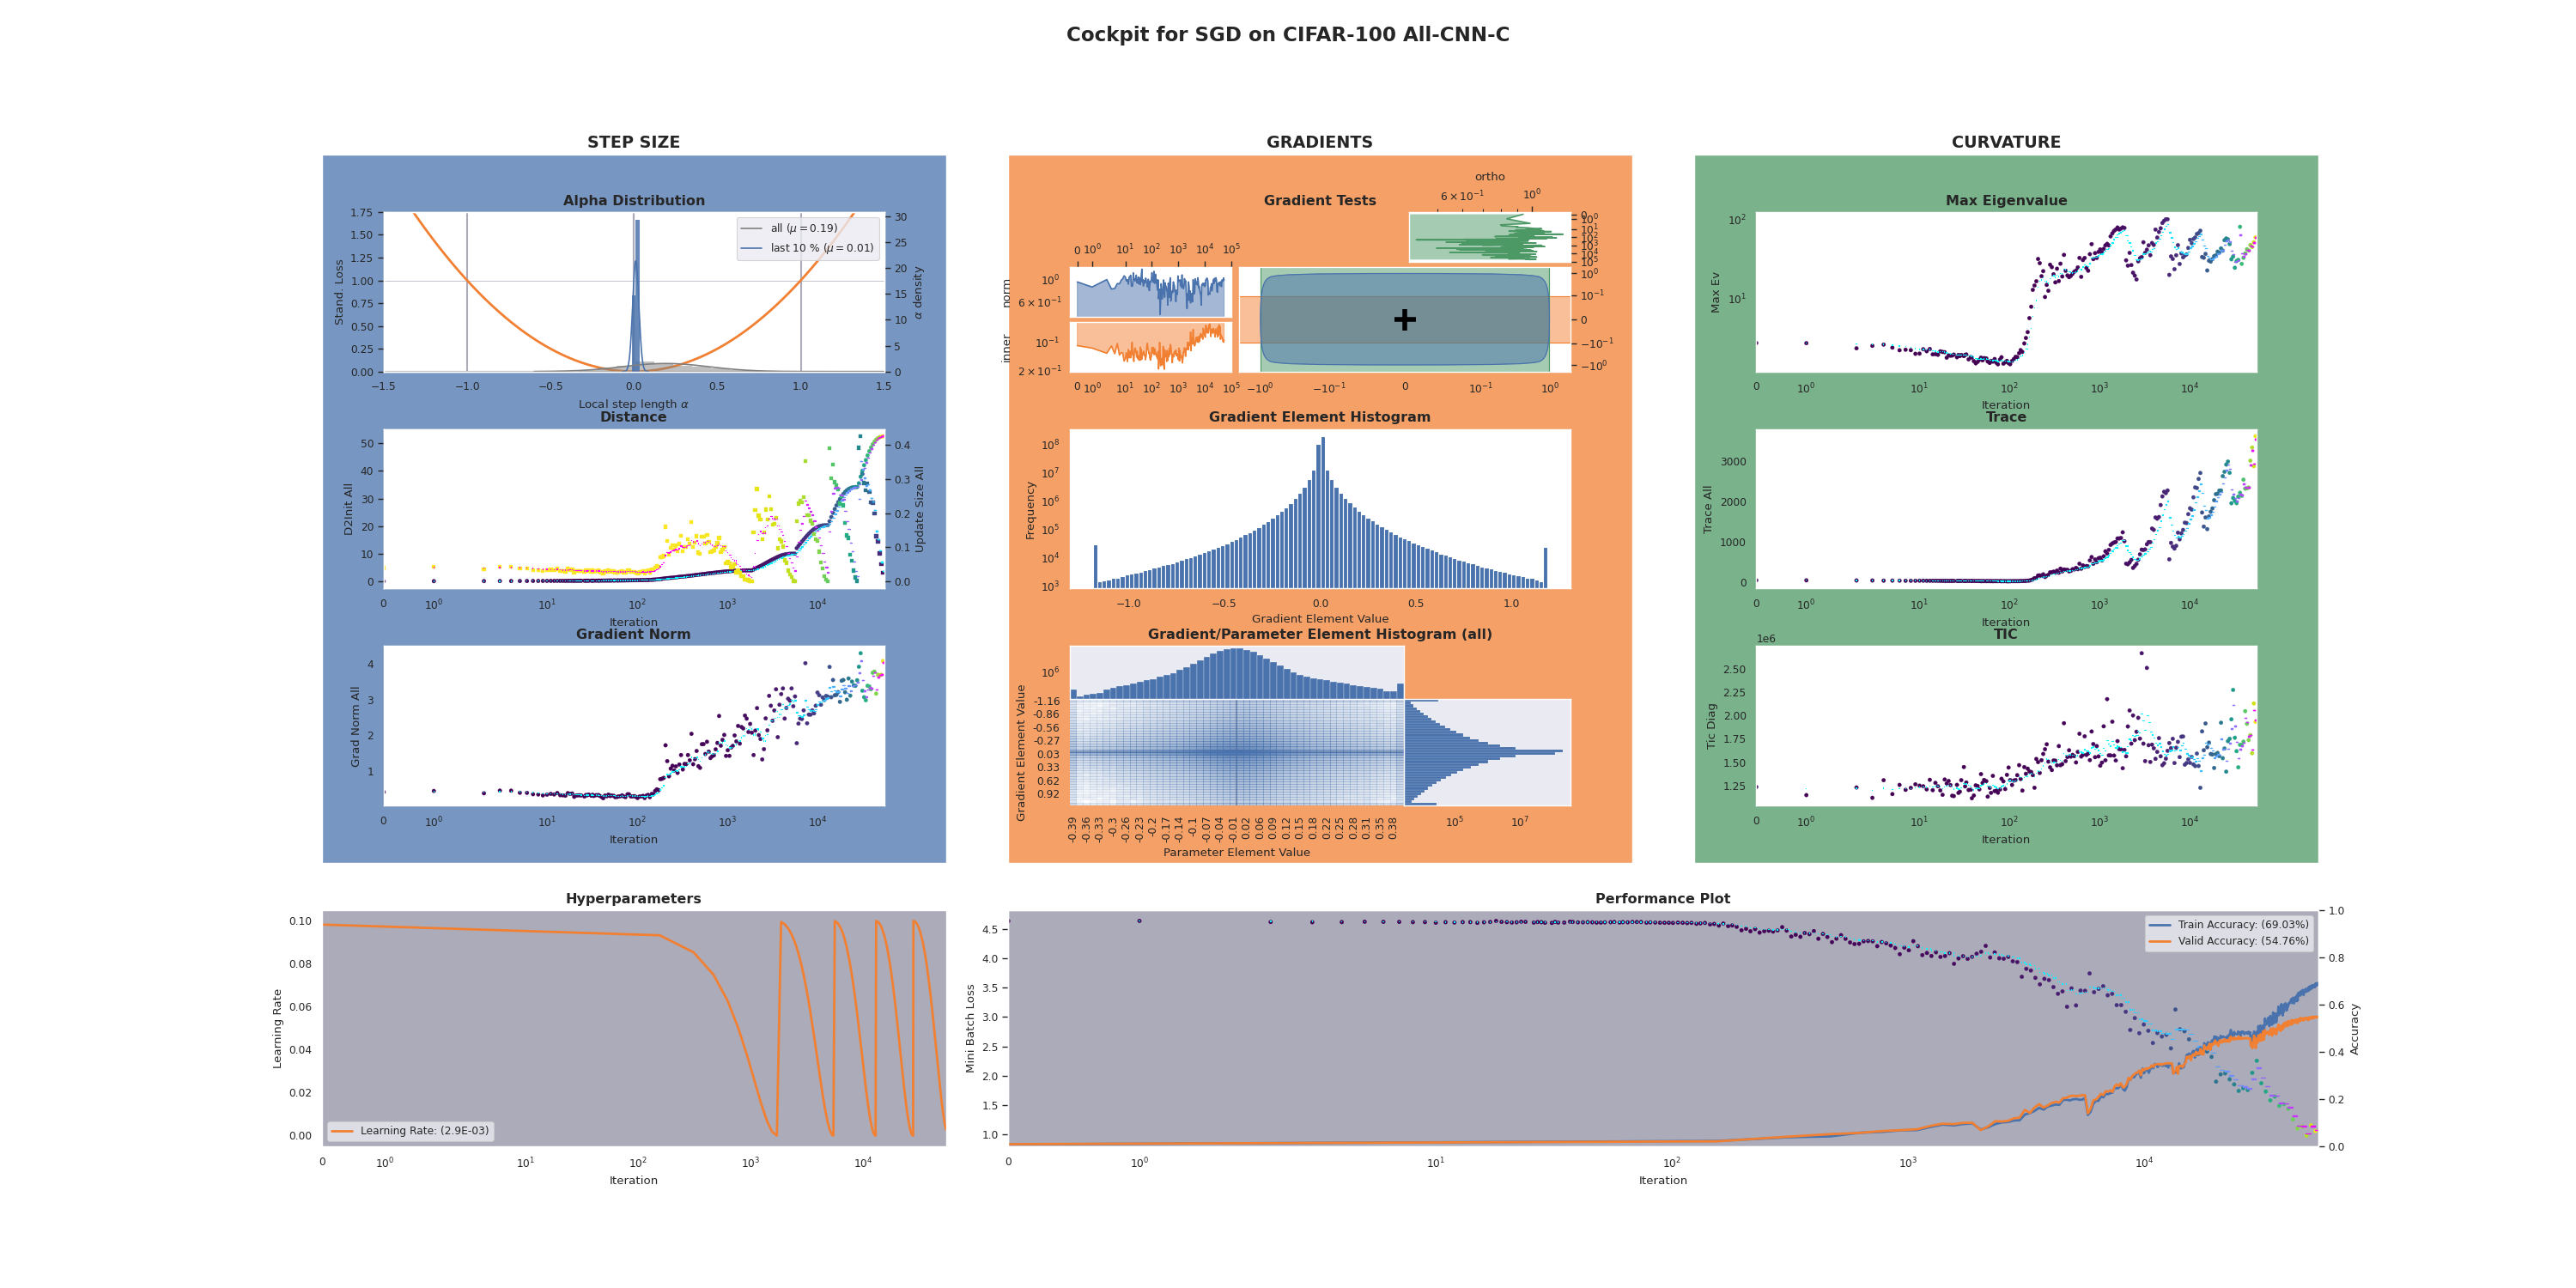
\includegraphics[width=0.97\linewidth, trim={7cm 2.5cm 5cm
      0.5cm}, clip]{../repos/cockpit-paper/tex/fig/10_showcase/cifar100_allcnnc_log.png}}
  \vspace{0.5ex}
  \caption{\textbf{Screenshot of \cockpittitle's full view} while training the
    \allcnnc \citep{springenberg2015striving} on \cifarhun with \sgd using a cyclical
    learning rate schedule. This figure and its labels are not meant to be
    legible, but rather give an impression of \cockpit's user experience. Gray
    panels (bottom row) show the information currently tracked by most
    practitioners. The individual instruments are discussed in
    \Cref{cockpit::sec:instruments}, and observations are described in
    \Cref{cockpit::sec:showcase}. An animated version can be found in the accompanying
    Github repository.}
  \label{cockpit::fig:showcase}
\end{figure*}

We aim to enrich the deep learning pipeline with a visual and statistical
debugging tool that uses newly proposed observables as well as several
established ones (\Cref{cockpit::sec:instruments}). We leverage and augment recent
extensions to AD (\ie \backpack \citep{dangel2020backpack} for
\pytorch \citep{paszke2019pytorch}) to efficiently access second-order statistical (\eg
gradient variances) and geometric (\eg Hessian) information. We show how these
quantities can aid the deep learning engineer in tasks, like learning rate
selection, as well as detecting common bugs with data processing or model
architectures (\Cref{cockpit::sec:experiments}).

Concretely, we introduce \cockpit, a flexible and efficient framework for
online-monitoring these observables during training in carefully designed plots
we call ``instruments'' (\Cref{cockpit::fig:showcase}). To practical, such
visualization must have a manageable computational overhead. We show that
\cockpit scales well to real-world deep learning problems (see
\Cref{cockpit::fig:showcase} and \Cref{cockpit::sec:showcase}). We also provide
three different configurations of varying computational complexity and
demonstrate that their instruments keep the computational cost \textit{well
  below} a factor of $2$ in run time (\Cref{cockpit::sec:benchmark}). It is
available as open-source code, extendable, and seamlessly integrates into
existing \pytorch training loops (\Cref{cockpit::app:code_example}).

%%% Local Variables:
%%% mode: latex
%%% TeX-master: "../thesis"
%%% End:


\section{\cockpittitle's Instruments}\label{cockpit::sec:instruments}
\subsubsection{Setting}

We consider supervised regression/classification with labeled data $(\vx, \vy)
\in \sX \times \sY$ generated by a distribution $\pdata(\vx, \vy)$. The training
set $\sD = \{ (\vx_n, \vy_n)\}_{n=1}^N$ consists of $N$ \iid samples from
$\pdata$ and the deep model $f_{\vtheta}: \sX \rightarrow \sF$ maps inputs
$\vx_n$ to predictions $f_{\vtheta}(\vx_n)$ by parameters $\vtheta \in \sTheta
:= \sR^D$. This prediction is evaluated by a loss function $\ell : \sF \times
\sY \rightarrow \R$ which compares to the label $\vy_n$. The goal is minimizing
an inaccessible expected risk $\gL_{\pdata}(\vtheta) = \int
\ell(f_{\vtheta}(\vx), \vy) \ \rd \pdata(\vx, \vy)$ by empirical approximation
through $\gL_{\sD}(\vtheta) = \nicefrac{1}{N} \sum_{n=1}^N
\ell(f_{\vtheta}(\vx_n), \vy_n) := \nicefrac{1}{N} \sum_{n=1}^N
\ell_n(\vtheta)$, which in practice is stochastically sub-sampled on
mini-batches $\sB \subset \sD$,
\begin{align}
  \label{cockpit::eq:mini-batch-loss}
  \gL_{\sB}(\vtheta) = \frac{1}{|\sB|} \sum_{(\vx_n,\vy_n) \in\sB} \ell_n(\vtheta)\,.
\end{align}
As is standard practice, we use first- and second-order information of the
mini-batch loss, described by its gradient $\vg_{\sB}(\vtheta)$ and Hessian
$\mH_{\sB}(\vtheta)$,
\begin{align}
  \vg_{\sB}(\vtheta)
  =
  \frac{1}{|\sB|} \sum_{(\vx_n, \vy_n) \in \sB}
  \grad{\vtheta}\ell_n(\vtheta)\, ,
  \quad
  \mH_{\sB}(\vtheta)
  =
  \frac{1}{|\sB|} \sum_{(\vx_n, \vy_n) \in \sB}
  \gradsquared{\vtheta} \ell_n(\vtheta)\,.
\end{align}

\subsubsection{Design Choices}

To minimize computational and design overhead, we restrict the metrics to
quantities that require no additional model evaluations. This means that, at
training step $t \to t + 1$ with mini-batches $\sB_t, \sB_{t+1}$ and parameters
$\vtheta_t, \vtheta_{t+1}$, we access information about the mini-batch losses
$\gL_{\sB_t}(\vtheta_t)$ and $\gL_{\sB_{t+1}}(\vtheta_{t+1})$, but no
cross-terms that require additional forward passes.

\subsubsection{Key Point}

$\gL_{\sB}(\vtheta), \vg_{\sB}(\vtheta)$, and $\mH_{\sB}(\vtheta)$ are just
expected values of a \textit{distribution} over the batch. Only recently, this
distribution has begun to attract attention \citep{faghri2020study} as its
computation has become more accessible \citep{bradbury2018jax,
  dangel2020backpack}. Contemporary optimizers leverage only the \emph{mean}
gradient and neglect higher moments. One core point of our work is making
extensive use of these distribution properties, trying to visualize them in
various ways. This distinguishes \cockpit from being ``just a collection of
plots'' that could be built in tools like \tensorboard. Leveraging these
distributional quantities, we create instruments and show how they can help
adapt hyperparameters (\Cref{cockpit::sec:adapting_hyperparameters}), analyze
the loss landscape (\Cref{cockpit::sec:curvature}), and track network dynamics
(\Cref{cockpit::sec:network_dynamics}). Instruments can sometimes be built from
already-computed information or are efficient variants of previously proposed
observables. To keep the presentation concise, we highlight the instruments
shown in \Cref{cockpit::fig:showcase} and listed in
\Cref{cockpit::tab:overview-quantities}. \Cref{cockpit::app:instruments} defines
them formally and contains more extensions, such as the mean \gsnr
\citep{liu2020understanding}, the early stopping \citep{mahsereci2017early} and
\cabs \citep{balles2017coupling} criterion, which can all be used in \cockpit.

{\def\arraystretch{1.2}
  \begin{table*}
    \caption{\textbf{Overview of \cockpittitle quantities}. They range from
      cheap byproducts, to nonlinear transformations of first-order information
      and Hessian-based measures. Some quantities have already been proposed,
      others are first to be considered in this work. They are categorized into
      configurations \textit{economy $\subseteq$ business $\subseteq$ full} based on their
      run time overhead (see \Cref{cockpit::sec:benchmark} for a detailed evaluation).}
    \label{cockpit::tab:overview-quantities}
    \begin{center}
      \footnotesize
      \begin{tabularx}{\linewidth}{lXcr}
        \toprule
        \textbf{Name}       & \textbf{Short Description}                                                                                           & \textbf{Config}   & \textbf{Pos.\,in Fig.\,\ref{cockpit::fig:showcase}}  \\
        \midrule
        \inlinecode{Alpha}      & Normalized step size on a noisy quadratic interpolation between $\vtheta_t$, $\vtheta_{t+1}$            & \textit{economy}  & top \textcolor{sns_blue}{left}        \\
        \inlinecode{Distance}   & Distance from initialization $\lVert \vtheta_{t} -  \vtheta_{0}  \rVert_2$                                           & \textit{economy}  & middle \textcolor{sns_blue}{left}     \\
        \inlinecode{UpdateSize} & Update size $\lVert \vtheta_{t + 1} - \vtheta_{t} \rVert_2$                                                          & \textit{economy}  & middle \textcolor{sns_blue}{left}     \\
        \inlinecode{GradNorm}   & Mini-batch gradient norm $\lVert \vg_{\sB}(\vtheta) \rVert_2$                                                        & \textit{economy}  & bottom \textcolor{sns_blue}{left}     \\
        \inlinecode{NormTest}   & Normalized fluctuations of residual norms ${\lVert  \vg_{\sB} - \vg_n \rVert_2}$, proposed in \citep{byrd2012sample}   & \textit{economy}  & top \textcolor{sns_orange}{center}    \\
        \inlinecode{InnerTest}  & Normalized fluctuations of $\vg_n$'s parallel to $\vg_{\sB}$, proposed in \citep{bollapragada2017adaptive} & \textit{economy}  & top \textcolor{sns_orange}{center}    \\
        \inlinecode{OrthoTest}  & Like  \inlinecode{InnerTest} but using the orthogonal components, proposed in \citep{bollapragada2017adaptive}                 & \textit{economy}  & top \textcolor{sns_orange}{center}    \\
        \inlinecode{GradHist1d} & Histogram of individual gradient elements, $\{[\vg_n]_j\}_{(\vx_{n},
                              \vy_{n}) \in \sB}^{j=1,\dots,D}$                           & \textit{economy}  & middle \textcolor{sns_orange}{center} \\
        \inlinecode{TICDiag}    & Relation of (diagonal) curvature and gradient noise, inspired by \citep{thomas2020interplay}                             & \textit{business} & bottom \textcolor{sns_green}{right}   \\
        \inlinecode{HessTrace}  & Exact or approximate Hessian trace, $\Tr(\mH_{\sB}(\vtheta))$, inspired by \citep{yao2020pyhessian}                           & \textit{business} & middle \textcolor{sns_green}{right}   \\
        \inlinecode{HessMaxEV}  & Maximum Hessian eigenvalue, $\lambda_{\text{max}}(\mH_{\sB}(\vtheta))$, inspired by \citep{yao2020pyhessian}                  & \textit{full}     & top \textcolor{sns_green}{right}      \\
        \inlinecode{GradHist2d} & Histogram of weights \& per-sample gradients, $\{
                              (\evtheta_j,[\vg_n]_j)\}_{(\vx_{n},
                              \vy_{n}) \in \sB}^{j=1,\dots,D}$  & \textit{full}     & bottom \textcolor{sns_orange}{center} \\
        \bottomrule
      \end{tabularx}
    \end{center}
  \end{table*}
}

%%% Local Variables:
%%% mode: latex
%%% TeX-master: "../../thesis"
%%% End:


\subsection{Adapting Hyperparameters}\label{cockpit::sec:adapting_hyperparameters}
One big challenge in deep learning is setting the hyperparameters correctly,
which is currently mostly done by trial \& error through parameter searches. We
aim to augment this process with instruments that inform the user about the
effect that the chosen parameters have on the current training process.

\subsubsection{\robustInlinecode{Alpha}: Are We Crossing the Valley?}

Using individual loss and gradient observations at the start and end point of
each iteration, we build a noise-informed uni-variate quadratic approximation
along the step direction (\ie the loss as a function of the step size), and
assess to which point on this parabola our optimizer moves. We standardize this
value $\alpha$ such that stepping to the valley-floor is assigned $\alpha=0$,
the starting point is at $\alpha=-1$ and updates to the point exactly opposite
of the starting point have $\alpha=1$ (see \Cref{cockpit::app:alpha} for a more
detailed visual and mathematical description of $\alpha$).
\Cref{cockpit::fig:LINE} illustrates the scenarios $\alpha=\pm1$ and how
monitoring the $\alpha$-distribution (right panel) can help distinguish between
two training runs with similar performance but distinct failure sources. By
default, this \cockpit instrument shows the $\alpha$-distribution for the last
10\,\% of training and the entire training process (top left plot in
\Cref{cockpit::fig:showcase}). In \Cref{cockpit::sec:alpha_exp} we show
empirically that, \emph{counter-intuitively}, it is generally \emph{not} a good
idea to choose the step size such that $\alpha$ is close to zero.

\subsubsection{Distances: Are We Making Progress?}

Another way to discern the trajectories in \Cref{cockpit::fig:LINE} is by
measuring the $L_2$ \textit{distance from initialization}
\citep{nagarajan2019generalization} and the \textit{update size}
\citep{agrawal2020investigating,frankle2020early} in parameter space. Both are
shown together in one \cockpit instrument (see also center-left plot in
\Cref{cockpit::fig:showcase}) and are far larger for the blue line in
\Cref{cockpit::fig:LINE}. These distance metrics are also able to disentangle
phases for the blue path. Using the same step size, it will continue to ``jump
back and forth'' between the loss valley's walls but at some point cease to make
progress. During this ``surfing of the walls'', the \textit{distance from
  initialization} increases, ultimately though, it will stagnate, with the
\textit{update size} remaining non-zero, indicating diffusion. While the initial
``surfing the wall''-phase benefits training (see
\Cref{cockpit::sec:alpha_exp}), achieving stationarity may require adaptation
once the optimizer reaches that diffusion.

\subsubsection{Gradient Norm: How Steep Is the Wall?}

The \textit{update size} will show that the orange trajectory is stuck. But why?
Such slow-down can result from both a bad learning rate and from loss landscape
plateaus. The \textit{gradient norm} (bottom left panel in
\Cref{cockpit::fig:showcase}) distinguishes these two causes.

\subsubsection{Gradient Tests: How Noisy Is the Batch?}

The batch size trades off gradient accuracy versus computational cost. Recently,
adaptive sampling strategies based on testing geometric constraints between mean
and individual gradients have been proposed
\citep{byrd2012sample,bollapragada2017adaptive}. The \textit{norm},
\textit{inner product}, and \textit{orthogonality tests} use a standardized
radius and two band widths (parallel and orthogonal to the gradient mean) that
indicate how strongly individual gradients scatter around the mean. The original
works use these values to adapt batch sizes. Instead, \cockpit combines all
three tests into a single gauge (top middle plot of
\Cref{cockpit::fig:showcase}) using the standardized noise radius and band
widths for visualization. These noise signals can be used to guide batch size
adaptation on- and offline, or to probe the influence of gradient alignment on
training speed \citep{sankararaman2020impact} and generalization
\citep{chatterjee2020coherent,chatterjee2020making,liu2020understanding}.

\subsection{Hessian Properties for Local Loss Geometry}\label{cockpit::sec:curvature}
An intuition for the local loss landscape helps in many ways. It can help
diagnose whether training is stuck, to adapt the step size, and explain
stability or regularization \citep{ginsburg2020regularization,jastrzebski2020break}. The key
challenge is the large number of weights: low-dimensional projections of
surfaces can behave unintuitively \citep{mulayoff2020unique}, but tracking the extreme
or average behaviors may help in debugging, especially if first-order metrics
fail.

\subsubsection{Hessian Eigenvalues: A Gorge or a Lake?}

In convex optimization, the maximum Hessian eigenvalue crucially determines the
appropriate step size \citep{schmidt2014convergence}. Many works have studied
the Hessian spectrum in machine learning
\citep[\eg][]{ghorbani2019investigation,ginsburg2020regularization,mulayoff2020unique,sagun2017eigenvalues,sagun2018empirical,yao2020pyhessian}.
In short: curvature matters. Established \citep{pearlmutter1994fast} and recent
autodiff frameworks \citep{dangel2020backpack} can compute Hessian properties
without requiring the full matrix. \cockpit leverages this to provide the
\textit{Hessian's largest eigenvalue} and \textit{trace} (right top and middle
plots in \Cref{cockpit::fig:showcase}). The former resembles the loss surface's
sharpest valley and can thus hint at training instabilities
\citep{jastrzebski2020break}. The \textit{trace} describes a notion of ``average
curvature'', since the eigenvalues $\lambda_i$ relate to it by $\sum_i \lambda_i
= \Tr(\mH_{\sB}(\vtheta))$, which might correlate with generalization
\citep{jastrzebski2021catastrophic}.

\subsubsection{TIC: How Do Curvature \& Gradient Noise Interact?}

There is an ongoing debate about curvature's link to generalization
\citep[\eg][]{dinh2017sharp,hochreiter1997flat,keskar2017large}. The
\emph{Takeuchi Information Criterion (TIC)}
\citep{takeuchi1976distribution,thomas2020interplay} estimates the
generalization gap by a ratio between Hessian and non-central second gradient
moment. It also provides intuition for changes in the objective function implied
by gradient noise. Inspired by \cite{thomas2020interplay}, \cockpit provides mini-batch TIC estimates (bottom
right plot of \Cref{cockpit::fig:showcase}).

\subsection{Visualizing Internal Network Dynamics}\label{cockpit::sec:network_dynamics}
Histograms are a natural visual compression of the high-dimensional $|\sB|
\times D$ individual gradient values. They give insights into the gradient
\emph{distribution} and hence offer a more detailed view of the learning signal.
Together with the parameter associated to each individual gradient, the entire
model status and dynamics can be visualized in a single plot and be monitored
during training. This provides a more fine-grained view of training compared to
tracking parameters and gradient norms \citep{frankle2020early}.

\subsubsection{Gradient \& Parameter Histograms: What Is Happening in Our Net?}

\cockpit offers a uni-variate \textit{histogram of the gradient elements}, \ie
the numbers
$\{[\vg_n( \vtheta )]_j\}_{(\vx_{n}, \vy_{n})\in \sB}^{j=1,\dots,D}$.
Additionally, a combined \textit{histogram of parameter-gradient pairs}
$\{([\vtheta]_j, [\vg_n( \vtheta )]_j\}_{(\vx_{n}, \vy_{n})\in \sB}^{j=1,\dots,D}$
provides a two-dimensional look into the network's gradient and parameter values
in a mini-batch. \Cref{cockpit::sec:misscaled_data_exp} shows an example
use-case of the gradient histogram; \Cref{cockpit::sec:vanishing_gradient_exp}
makes the case for the layer-wise variants of the instruments.

%%% Local Variables:
%%% mode: latex
%%% TeX-master: "../thesis"
%%% End:


\section{Experiments}\label{cockpit::sec:experiments}
The diverse information provided by \cockpit can help users and researchers in
many ways, some of which, just like for a traditional debugger, only become
apparent in practical use. In this section, we present a few motivating
examples, selecting specific instruments and scenarios in which they are
practically useful. Specifically, we show that \cockpit can help the user
discern between, and thus fix, common training bugs
(\Cref{cockpit::sec:misscaled_data_exp,cockpit::sec:vanishing_gradient_exp}) that are otherwise
hard to distinguish as they lead to the same failure: bad training. We
demonstrate that \cockpit can guide practitioners to choose efficient
hyperparameters \emph{within a single training run}
(\Cref{cockpit::sec:vanishing_gradient_exp,cockpit::sec:alpha_exp}). Finally, we highlight that
\cockpit's instruments can provide research insights about the optimization
process (\Cref{cockpit::sec:alpha_exp}). Our empirical findings are demonstrated on
problems from the \deepobs \citep{schneider2019deepobs} benchmark collection.

\subsection{Incorrectly Scaled Data}\label{cockpit::sec:misscaled_data_exp}
One prominent source of bugs is the data pipeline. To pick a relatively simple
example: for standard optimizers to work at their usual learning rates, network
inputs must be standardized (\ie~between zero and one, or have zero mean and
unit variance \citep[\eg][]{bengio2012neural}). If the user forgets to do this,
optimizer performance is likely to degrade. It can be difficult to identify the
source of this problem as it does not cause obvious failures, \texttt{NaN} or
\texttt{Inf} gradients, \etc. We now construct a semi-realistic example, to show
how using \cockpit can help diagnose this problem upon observing slow training
performance.

By default\sidenote{See the documentation, available at
  \href{https://www.cs.toronto.edu/~kriz/cifar.html}{\texttt{cs.toronto.edu/\textasciitilde
      kriz/cifar.html}}}, the popular image datasets \cifartenhun
\citep{krizhevsky2009learning} are provided as \numpy \citep{harris2020array}
arrays that consist of integers in the interval $[0,255]$. This \emph{raw} data,
instead of the widely used version with floats in $[0,1]$, changes the data
scale and thus the gradients by a factor of $255$. Therefore, the optimizer's
optimal learning rate is scaled as well. In other words, the default parameters
of popular optimization methods may not work well anymore, or good
hyperparameters may take extreme values. Even if the user directly inspects the
training images, this may not be apparent
(\Cref{cockpit::fig:data-pre-processing}). But the gradient histogram instrument
of \cockpit, which has a deliberate default plotting range around $[-1,1]$ to
highlight such problems, immediately and prominently shows that there is an
issue.

\begin{figure}
%	 pgfplots style "prerocessingexperimentdefault"
		\pgfkeys{/pgfplots/preprocessingexperimentdefault/.style={
				width=\linewidth,
				height=1.4\linewidth,
				every axis plot/.append style={line width = 1.2pt},
				tick pos = left,
				xmajorticks = true,
				ymajorticks = true,
				ylabel near ticks,
				xlabel near ticks,
				xtick align = inside,
				ytick align = inside,
				legend cell align = left,
				legend columns = 1,
				legend pos = south east,
				legend style = {
					fill opacity = 0.9,
					text opacity = 1,
					font = \small,
				},
				xticklabel style = {font = \small, inner xsep = -5ex},
				xlabel style = {font = \small},
				axis line style = {black},
				yticklabel style = {font = \small, inner ysep = -4ex},
				ylabel style = {font = \small},
				title style = {font = \small, inner ysep = -3ex},
				grid = major,
				grid style = {dashed}
			}
		}
	
	\centering
	\begin{subfigure}[t]{0.46\textwidth}
		\begin{minipage}{.49\textwidth}
			\Cshadowbox{
\includegraphics[width = .35\textwidth]{fig/06_preprocessing/fig_samples/cifar10raw_3c3d_sample_00.png}}
			\Cshadowbox{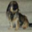
\includegraphics[width = .35\textwidth]{fig/06_preprocessing/fig_samples/cifar10raw_3c3d_sample_01.png}}
	
			\Cshadowbox{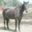
\includegraphics[width = .35\textwidth]{fig/06_preprocessing/fig_samples/cifar10raw_3c3d_sample_02.png}}
			\Cshadowbox{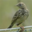
\includegraphics[width = .35\textwidth]{fig/06_preprocessing/fig_samples/cifar10raw_3c3d_sample_03.png}}
		\end{minipage}
		\begin{minipage}{.49\textwidth}
			\centering
			%			 customize "zmystyle" as you wish
			\pgfkeys{/pgfplots/zmystyle/.style={preprocessingexperimentdefault,
					ylabel={Gradient Element}
			}}
			\vspace{1.4\baselineskip}
			\input{fig/06_preprocessing/fig_histograms/cifar10raw_3c3d.tex}
		\end{minipage}
		\caption{Normalized Data}
		\label{fig:data-pre-processing_norm}
	\end{subfigure}
	\hfill
	\begin{subfigure}[t]{0.46\textwidth}
		\begin{minipage}{.49\textwidth}
			\Cshadowbox{
\includegraphics[width = .35\textwidth]{fig/06_preprocessing/fig_samples/cifar10scale255_3c3d_sample_00.png}}
			\Cshadowbox{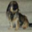
\includegraphics[width = .35\textwidth]{fig/06_preprocessing/fig_samples/cifar10scale255_3c3d_sample_01.png}}
			
			\Cshadowbox{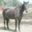
\includegraphics[width = .35\textwidth]{fig/06_preprocessing/fig_samples/cifar10scale255_3c3d_sample_02.png}}
			\Cshadowbox{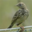
\includegraphics[width = .35\textwidth]{fig/06_preprocessing/fig_samples/cifar10scale255_3c3d_sample_03.png}}
		\end{minipage}
		\begin{minipage}{.49\textwidth}
			\centering
%			 customize "zmystyle" as you wish
			\pgfkeys{/pgfplots/zmystyle/.style={preprocessingexperimentdefault,
					ylabel={Gradient Element}
			}}
			\vspace{1.4\baselineskip}
			\input{fig/06_preprocessing/fig_histograms/cifar10scale255_3c3d.tex}
		\end{minipage}
		\caption{Raw Data}
		\label{fig:data-pre-processing_raw}
	\end{subfigure}
	\caption{\textbf{Same inputs, different gradients; Catching data 
	    bugs with \cockpittitle.} (a) \emph{normalized} ($[0, 1]$) and (b)
    	\emph{raw} $([0, 255])$ images look identical in auto-scaled
	    front-ends like \matplotlib's \texttt{imshow}. The gradient distribution on
	    the \threecthreed model, however, is crucially affected by this
	    scaling.}
	\label{fig:data-pre-processing}
\end{figure}

%%% Local Variables:
%%% mode: latex
%%% TeX-master: "../cockpit_paper"
%%% End:


Of course, this particular data is only a placeholder for real practical data
sets. While this problem may not frequently arise in the highly pre-processed,
packaged \cifarten, it is not a rare problem for practitioners who work with
their personal datasets. This is particularly likely in domains outside
standard computer vision, \eg when working with mixed-type data without obvious
natural scales.

\subsection{Vanishing Gradients}\label{cockpit::sec:vanishing_gradient_exp}

The model itself can be a source of training bugs. As before, such problems
mostly arise with novel datasets, where well-working architectures are unknown.
The following example shows how even small (in terms of code) model
modifications may severely harm the training.

\Cref{cockpit::fig:layerwise-experiment_net} shows the distribution of gradient values of
two different network architectures in blue and orange. Although the blue model
trains considerably better than the orange one, their gradient distributions
look quite similar. The difference becomes evident when inspecting the histogram
\emph{layer-wise}. We can see that multiple layers have a degenerated gradient
distribution with many elements being practically zero (see
\Cref{cockpit::fig:layerwise-experiment_layers}, bottom row). Since the fully connected
layers close to the output have far more parameters (a typical pattern of
convolutional networks), they dominate the network-wide histogram. This obscures
that a major part of the model is effectively unable to train.

\begin{figure}
%	 pgfplots style "layerwiseexperimentdefault"
	  \pgfkeys{/pgfplots/layerwiseexperimentdefault/.style={
	      width=\linewidth,
	      height=0.13\textheight,
	      every axis plot/.append style={line width = 1.2pt},
	      tick pos = left,
	      xmajorticks = true,
	      ymajorticks = true,
	      ylabel near ticks,
	      xlabel near ticks,
	      xtick align = inside,
	      ytick align = inside,
	      ytick={-1,0,1},
	      legend cell align = left,
	      legend columns = 1,
	      legend pos = south east,
	      legend style = {
	        fill opacity = 0.9,
	        text opacity = 1,
	        font = \small,
	      },
	      xticklabel style = {font = \small, inner xsep = -5ex},
	      xlabel style = {font = \small},
	      axis line style = {black},
	      yticklabel style = {font = \small, inner ysep = -4ex},
	      ylabel style = {font = \small},
	      title style = {font = \small, inner ysep = -3ex},
	      grid = major,
	      grid style = {dashed}
	    }
	  }
	
	\centering
	\begin{subfigure}[t]{0.4\textwidth}
%		 customize "zmystyle" as you wish
		\pgfkeys{/pgfplots/zmystyle/.style={layerwiseexperimentdefault,
		   title = {Network}, ylabel=Gradient\\Element, ylabel style={align=left}, xticklabels = {}
		 }}
		\input{fig/09_layerwise/net-grad-margin-cifar10_3c3d.tex}
		
		\vspace{-0.1cm}
%		customize "zmystyle" as you wish
		\pgfkeys{/pgfplots/zmystyle/.style={layerwiseexperimentdefault,
		   ylabel=Gradient\\Element, ylabel style={align=left}
		 }}
		\input{fig/09_layerwise/net-grad-margin-cifar10_3c3dsig.tex}
		\caption{Network Histogram}
		\label{fig:layerwise-experiment_net}
	\end{subfigure}
	\hfill
	\begin{subfigure}[t]{0.57\textwidth}
		    \pgfkeys{/pgfplots/layerwiseexperimentdefaultparameters/.style={
		        layerwiseexperimentdefault,
		        ylabel={},
		        ylabel style = {inner ysep = -4ex},
		        yticklabels={},
		        width=0.45\textwidth,
		      }
		    }
		    \hfill%
		    \pgfkeys{/pgfplots/zmystyle/.style={layerwiseexperimentdefaultparameters,
		        title={Parameter 0}, xticklabels = {},}}%
		    \input{fig/09_layerwise/param-0-grad-margin-cifar10_3c3d.tex}
		    \hfill
		    \pgfkeys{/pgfplots/zmystyle/.style={layerwiseexperimentdefaultparameters,
		        title={Parameter 4}, xticklabels = {},}}%
		    \input{fig/09_layerwise/param-4-grad-margin-cifar10_3c3d.tex}
		    \pgfkeys{/pgfplots/zmystyle/.style={layerwiseexperimentdefaultparameters,
		        title={Parameter 10}, xticklabels = {},}}%
		    \hfill
		    \input{fig/09_layerwise/param-10-grad-margin-cifar10_3c3d.tex}
		    \hfill
		
		    \vspace{-0.1cm}\hspace{-0.25\baselineskip}\hfill
		    \pgfkeys{/pgfplots/zmystyle/.style={layerwiseexperimentdefaultparameters}}
		    \input{fig/09_layerwise/param-0-grad-margin-cifar10_3c3dsig.tex}
		    \hfill
		    \input{fig/09_layerwise/param-4-grad-margin-cifar10_3c3dsig.tex}
		    \hfill
		    \input{fig/09_layerwise/param-10-grad-margin-cifar10_3c3dsig.tex}
		    \hfill
		\caption{Layer-wise Histograms}
		\label{fig:layerwise-experiment_layers}
	\end{subfigure}
	\caption{\textbf{Gradient distributions of two similar architectures on the 
		same problem}. (a) Distribution of individual gradient elements 
		summarized over the entire network. Both seem similar.
		(b) Layer-wise histograms for a subset of layers. Parameter 0 is the layer 
		closest to the network's input, parameter 10 closest to its output. 
		Only the layer-wise view reveals that there are several degenerated gradient 
		distributions for the orange network making training unnecessary hard.}
	\label{fig:layerwise-experiment}
\end{figure}


%%% Local Variables:
%%% mode: latex
%%% TeX-master: "../cockpit_paper"
%%% End:


Both the blue and orange networks follow \deepobs's \threecthreed architecture.
The only difference is the non-linearity: the blue net uses standard ReLU
activations, while the orange one has sigmoid activations. Here, the layer-wise
histogram instrument of \cockpit~highlights which part of the architecture makes
training unnecessarily hard. Accessing information layer-wise is also essential
due to the strong overparameterization in deep models where training can happen
in small subspaces \citep{gurari2018gradient}. Again, this is hard to do with
common monitoring tools, such as the loss curve.

\subsection{Tuning Learning Rates}
\label{cockpit::sec:alpha_exp}
Once the architecture is defined, the optimizer's learning rate is the most
important hyperparameter to tune. Getting it right requires extensive
hyperparameter searches at high resource costs. \cockpit's instruments can
provide intuition and information to streamline this process: in contrast to the
raw learning rate, the curvature-standardized step size $\alpha$-quantity (see
\Cref{cockpit::sec:adapting_hyperparameters}) has a natural scale.

\begin{figure*}
	\begin{center}
		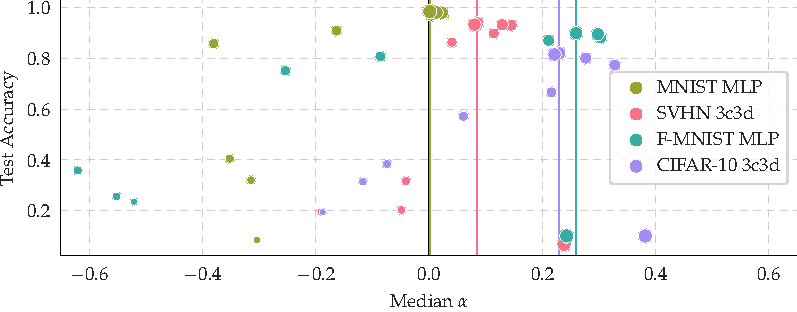
\includegraphics[width=\linewidth]{../repos/cockpit-paper/fig/07_learning_rate_selection/output/median_alpha_vs_performance_thesis-wide}
	\end{center}
  \vspace{-2ex}
	\caption{\textbf{Test accuracy as a function of standardized step size
      $\alpha$}. For four \deepobs problems (see \Cref{cockpit::app:benchmarks}), final
    test accuracy is shown versus the median $\alpha$-value over the entire
    training. Marker size indicates the magnitude of the raw learning rate,
    marker color identifies tasks (see legend). For each problem, the
    best-performing setting is highlighted by a vertical colored line.}
	\label{cockpit::fig:alpha_exp}
\end{figure*}

Across multiple optimization problems, we observe, perhaps surprisingly, that
the best runs and indeed all good runs have a median $\alpha>0$
(\Cref{cockpit::fig:alpha_exp}). This illustrates a fundamental difference between
stochastic optimization, as is typical for machine learning, and classic
deterministic optimization. Instead of locally stepping ``to the valley floor''
(optimal in the deterministic case), stochastic optimizers should
\emph{overshoot} the valley somewhat. This need to ``surf the walls'' has been
hypothesized before \citep[e.g.][]{wu2018understanding,xing2018walk} as a property of neural
network training. Frequently, learning rates are adapted during training, which
fits with our observation about positive $\alpha$-values: ``overshooting''
allows fast early progression towards areas of lower loss, but it does not yield
convergence in the end. Real-time visualizations of the training state, as
offered by \cockpit, can augment these fine-tuning processes.

\Cref{cockpit::fig:alpha_exp} also indicates a major challenge preventing simple
automated tuning solutions: the optimal $\alpha$-value is problem-dependent, and
simpler problems, such as a multi-layer perceptron (\mlp) on \mnist
\citep{lecun1998gradient}, behave much more similar to classic optimization problems.
Algorithmic research on small problems can thus produce misleading conclusions.
The figure also shows that the $\alpha$-gauge is not sufficient by itself:
extreme overshooting with a too-large learning rate leads to poor performance,
which however can be prevented by taking additional instruments into account.
This makes the case for the cockpit metaphor of increasing interpretability from
several instruments in conjunction. By combining the $\alpha$-instrument with
other gauges that capture the local geometry or network dynamics, the user can
better identify good choices of the learning rate and other hyperparameters.

%%% Local Variables:
%%% mode: latex
%%% TeX-master: "../thesis"
%%% End:


\section{Showcase}\label{cockpit::sec:showcase}
Having introduced the tool, we can now return to \Cref{cockpit::fig:showcase}
for a closer look. The figure shows a snapshot from training the \allcnnc
\citep{springenberg2015striving} on \cifarhun using \sgd with a cyclic learning
rate schedule (bottom left panel). Diagonal curvature instruments are configured
to use an MC approximation to save run time (here, $C=100$, compare
\Cref{cockpit::sec:benchmark}).

A glance at all panels shows that the learning rate schedule is reflected in the
metrics. However, the instruments also provide insights into the early phase of
training (first $\sim100$ iterations), where the learning rate is still
unaffected by the schedule: there, the loss plateaus and the optimizer takes
relatively small steps (compared to later, as can be seen in the small gradient
norms, and small distance from initialization). Based on these low-cost
instruments, one may thus at first suspect that training was poorly initialized;
but training indeed succeeds after iteration 100! Viewing \cockpit entirely
though, it becomes clear that optimization in these first steps is not stuck at
all: while loss, gradient norms, and distance in parameter space remain almost
constant, curvature changes, which expresses itself in a clear downward trend of
the maximum Hessian eigenvalue (top right panel).

The importance of early training phases has recently been hypothesized
\citep{frankle2020early}, suggesting a logarithmic timeline. Not only does our
showcase support this hypothesis, but it also provides an explanation from the
curvature-based metrics, which in this particular case are the only meaningful
feedback in the first few training steps. It also suggests monitoring training
at log-spaced intervals. \cockpit provides the flexibility to do so, indeed,
\Cref{cockpit::fig:showcase} has been created with log-scheduled tracking events.

As a final note, we recognize that the approach taken here promotes an amount of
\emph{manual} work (monitoring metrics, deliberately intervening, \etc) that may
seem ironic and at odds with the paradigm of automation that is at the heart of
machine learning. However, we argue that this might be what is needed at this
point in the evolution of the field. Deep learning has been driven notably by
scaling compute resources \citep{thompson2020computational}, and fully automated
one-shot training may still be some way out. To develop better training methods,
researchers, not just users, need \emph{algorithmic} interpretability and
explainability: direct insights and intuition about the processes taking place
``inside'' neural nets. To highlight how \cockpit might provide this, we
contrast in \Cref{cockpit::app:convex-problems} the view of two convex \deepobs
problems (noisy quadratic \& logistic regression on \mnist). In both cases, the
instruments behave differently compared to the deep learning problem in
\Cref{cockpit::fig:showcase}. In particular, the gradient norm increases (left
column, bottom panel) during training, and individual gradients become less
scattered (center column, top panel). This is diametrically opposed to the
convex problems and shows that deep learning differs even qualitatively from
well-understood optimization problems.

%%% Local Variables:
%%% mode: latex
%%% TeX-master: "../thesis"
%%% End:


\section{Benchmark}\label{cockpit::sec:benchmark}
\Cref{cockpit::sec:experiments} made a case for \cockpit as an effective debugging and
tuning tool. To make the library useful in practice, it must also have limited
computational cost. We now show that it is possible to compute all quantities at
reasonable overhead. The user can control the absolute cost along two
dimensions, by reducing the number of instruments, or by reducing their update
frequency.

All benchmark results show \sgd without momentum. \cockpit's quantities,
however, work for generic optimizers and can mostly be used identically without
increased costs. One current exception is \inlinecode{Alpha} which can be
computed more efficiently given the update rule.\sidenote{This is currently
  implemented for vanilla \sgd. Otherwise, \cockpit falls back to a less
  efficient scheme.}

\subsubsection{Complexity Analysis}

Computing more information adds computational overhead, of course. However,
recent work \citep{dangel2020backpack} has shown that first-order information,
like distributional statistics on the batch gradients, can be computed on top of
the mean gradient at little extra cost. Similar savings apply for most
quantities in \Cref{cockpit::tab:overview-quantities}, as they are
\mbox{(non-)linear} transformations of individual gradients. A subset of
\cockpit's quantities also uses second-order information from the Hessian
diagonal. For ReLU networks on a classification task with $C$ classes, the
additional work is proportional to $C$ gradient backpropagations (\ie $C=10$ for
\cifarten, $C=100$ for \cifarhun). Parallel processing can, to some extent,
process these extra backpropagations in parallel without significant overhead.
If this is no longer possible, we can fall back to a Monte Carlo (MC) sampling
approximation, which reduces the number of extra backprop passes to the number
of samples (1 by default).\sidenote{An MC-sampled approximation of the
  Hessian/generalized Gauss-Newton has been used in \Cref{cockpit::fig:showcase}
  to reduce the prohibitively large number of extra backprops on \cifarhun
  ($C=100$).}

While parallelization is possible for the gradient instruments, computing the
maximum Hessian eigenvalue is inherently sequential. Similar to
\citet{yao2020pyhessian}, we use matrix-free Hessian-vector products by
automatic differentiation \citep{pearlmutter1994fast}, where each product's
costs are proportional to one gradient computation. Regardless of the underlying
iterative eigensolver, multiple such products must be queried to compute the
spectral norm (the number depends on the spectral gap to the second-largest
eigenvalue).

\subsubsection{Run Time Benchmark}

\Cref{cockpit::fig:benchmark-instruments} shows the wall-clock computational
overhead for individual instruments (details in
\Cref{cockpit::app:benchmarks}).\sidenote{To improve readability, we exclude
  \inlinecode{HessMaxEV} here, because its overhead is large compared to other
  quantities. Surprisingly, we also observed significant cost for the 2D
  histogram on GPU. It is caused by an implementation bottleneck for histogram
  shapes observed in deep models. We thus also omit \inlinecode{GradHist2d}
  here, as we expect it to be eliminated with future implementations (see
  \Cref{cockpit::app:run-time-benchmarks} for a detailed analysis and further
  benchmarks). Both quantities, however, are part of the benchmark shown in
  \Cref{cockpit::fig:benchmark_heatmap}.} As expected, byproducts are virtually
free, and quantities that rely solely on first-order information add little
overhead (at most roughly 25\,\% on this problem). Thanks to parallelization,
the ten extra backward passes required for Hessian quantities reduce to less
than 100\,\% overhead. Individual overheads also do not simply add up when
multiple quantities are tracked, because quantities relying on the same
information share computations.

\begin{figure*}
  \centering
  \begin{subfigure}[t]{0.6\linewidth}
    \centering
    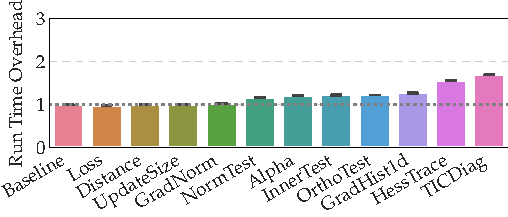
\includegraphics[width=\linewidth]{../repos/cockpit-paper/fig/01_benchmark/output/fig_individual/benchmark_cifar10_3c3d_cuda_thesis-wide}
    \caption{Overhead \cockpit instruments}
    \label{cockpit::fig:benchmark-instruments}
  \end{subfigure}
  \hfill
  \begin{subfigure}[t]{0.35\linewidth}
    \centering
    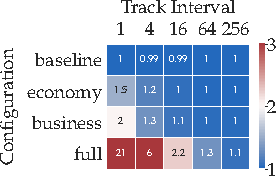
\includegraphics[width=\linewidth]{../repos/cockpit-paper/fig/01_benchmark/output/fig_grid/benchmark_cifar10_3c3d_cuda_thesis-wide}
    \caption{Overhead \cockpit configurations}
    \label{cockpit::fig:benchmark_heatmap}
  \end{subfigure}
  \caption{\textbf{Run time overhead for individual \cockpittitle instruments
      and configurations} as shown on \cifarten \threecthreed on a GPU.
    \subfigref{cockpit::fig:benchmark-instruments} The run time overheads for
    individual instruments are shown as multiples of the \emph{baseline} (no
    tracking). Most instruments add little overhead. This plot shows the
    overhead in one iteration, determined by averaging over multiple iterations
    and random seeds. \subfigref{cockpit::fig:benchmark_heatmap} Overhead for
    different \cockpit configurations. Adjusting the tracking interval and
    re-using the computation shared by multiple instruments can make the
    overhead orders of magnitude smaller. Blue fields mark settings that allow
    tracking without doubling the training time.}
  \label{cockpit::fig:benchmark}
\end{figure*}

To allow a rough cost control, \cockpit currently offers three configurations,
called \inlinecode{``economy''}, \inlinecode{``business''}, and
\inlinecode{``full''}, in increasing order of cost
(\Cref{cockpit::tab:overview-quantities}). As a basic guideline, we consider a
factor of two to be an acceptable limit for the increase in training time and
benchmark the configurations' run times for different tracking intervals.
\Cref{cockpit::fig:benchmark_heatmap} shows a run time matrix for the \cifarten
\threecthreed problem, where settings that meet this limit are set in blue (more
problems including \imagenet are shown in \Cref{cockpit::app:benchmarks}).
Speedups due to shared computations are easy to read off: summing all the
individual overheads shown in \Cref{cockpit::fig:benchmark-instruments} would
result in a total overhead larger than 200\,\%, while the joint overhead
(\textit{business}) reduces to 140\,\%. The \textit{economy} configuration can
easily be tracked at every step of this problem and stay well below our
threshold of doubling the execution time. \cockpit's full view, shown in
\Cref{cockpit::fig:showcase}, can be updated every $64$-th iteration without a
major increase in training time (this corresponds to about five updates per
epoch). Finally, tracking any configuration about once per epoch---which is
common in practice---adds overhead close to zero (rightmost column).

This good performance is largely due to the efficiency of the \backpack package
\citep{dangel2020backpack}, which we leverage with custom and optimized modification,
that compacts information layer-wise and then discards unneeded buffers. Using
layer-wise information (\Cref{cockpit::sec:vanishing_gradient_exp}) scales better to
large networks, where storing the entire model's individual gradients all at
once becomes increasingly expensive (see \Cref{cockpit::app:benchmarks}). To the best of
our knowledge, many of the quantities in \Cref{cockpit::tab:overview-quantities},
especially those relying on individual gradients, have only been explored on
rather small problems. With \cockpit they can now be accessed at a reasonable
rate for deep learning models outside the toy problem category.

%%% Local Variables:
%%% mode: latex
%%% TeX-master: "../thesis"
%%% End:


\section{Conclusion}\label{cockpit::sec:conclusion}
Contemporary machine learning, in particular deep learning, remains a craft and
an art. High dimensionality, stochasticity, and non-convexity require constant
tracking and tuning, often resulting in a painful process of trial and error.
When things fail, popular performance measures, like the training loss, do not
provide enough information by themselves. These metrics only tell \emph{whether}
the model is learning, but not \emph{why}. Alternatively, traditional debugging
tools can provide access to individual weights and data. However, in models
whose power only arises from possessing myriad weights, this approach is
hopeless, like looking for the proverbial needle in a haystack.

To mitigate this, we proposed \cockpit, a practical visual debugging tool for
deep learning. It offers instruments to monitor the network's internal dynamics
during training, in real-time. In its presentation, we focused on two crucial
factors affecting user experience: Firstly, such a debugger must provide
meaningful insights. To demonstrate \cockpit's utility, we showed how it can
identify bugs where traditional tools fail. Secondly, it must come at a feasible
computational cost. Although \cockpit uses rich second-order information,
efficient computation keeps the necessary run time overhead cheap. The
open-source \pytorch package can be added to many existing training loops.

Obviously, such a tool is never complete. Just like there is no perfect
universal debugger, the list of current instruments is naturally incomplete.
Further practical experience with the tool, for example in the form of a future
larger user study, could provide additional evidence for its utility. However,
our analysis shows that \cockpit provides useful tools and extracts valuable
information presently not accessible to the user. We believe that this improves
algorithmic interpretability -- helping practitioners understand how to make
their models work -- but may also inspire new research. The code is designed
flexibly, deliberately separating the computation and visualization. New
instruments can be added easily and also be shown by the user's preferred
visualization tool, \eg \tensorboard. Of course, instead of just showing the
data, the same information can be used by novel algorithms directly,
side-stepping the human in the loop.

%%% Local Variables:
%%% mode: latex
%%% TeX-master: "../thesis"
%%% End:


\section*{Acknowledgments}
The authors gratefully acknowledge financial support by the European Research
Council through ERC StG Action 757275 / PANAMA; the DFG Cluster of Excellence
“Machine Learning - New Perspectives for Science”, EXC 2064/1, project number
390727645; the German Federal Ministry of Education and Research (BMBF) through
the Tübingen AI Center (FKZ: 01IS18039A); and funds from the Cyber Valley
Initiative of the Ministry for Science, Research and Arts of the State of
Baden-Württemberg. Moreover, the authors thank the International Max Planck
Research School for Intelligent Systems (IMPRS-IS) for supporting Felix Dangel
and Frank Schneider. Further, we are grateful to Agustinus Kristiadi, Alexandra
Gessner, Christian Fröhlich, Filip de Roos, Jonathan Wenger, Julia Grosse, Lukas
Tatzel, Marius Hobbhahn, and Nicholas Krämer for providing feedback to the
manuscript.

%%% Local Variables:
%%% mode: latex
%%% TeX-master: "../thesis"
%%% End:


\setchapterpreamble[u]{\margintoc}
\chapter[ViViT: Curvature Access Through the \ggn's Low-rank Structure]{ViViT:
  Curvature Access Through the Generalized Gauss-Newton's Low-rank
  Structure}\label{chap:vivit}
\subsubsection{Abstract}

Curvature in form of the Hessian or its generalized Gauss-Newton (\ggn)
approximation is valuable for algorithms that rely on a local model for the loss
to train, compress, or explain deep networks.
% What has been done
Existing methods based on implicit multiplication via automatic differentiation
or Kronecker-factored block diagonal approximations do not consider noise in the
mini-batch.
% What we do
We present \vivit, a curvature model that leverages the \ggn's low-rank
structure without further approximations. It allows for efficient computation of
eigenvalues, eigenvectors, as well as per-sample first- and second-order
directional derivatives.
% Computation
The representation is computed in parallel with gradients in one backward pass
and offers a fine-grained cost-accuracy trade-off, which allows it to scale.
% Experiments
We demonstrate this by conducting performance benchmarks and substantiate
\vivit's usefulness by studying the impact of noise on the \ggn's structural
properties during neural network training.

\marginnote{%
  \begin{center}
    Code and experiments available at the Github repositories
    \href{https://github.com/f-dangel/vivit}{\texttt{f-dangel/vivit}},
    \href{https://github.com/f-dangel/vivit-experiments}{\texttt{f-dangel/vivit-experiments}}
  \end{center}
  \begin{center}
    
\includegraphics[height =
    0.8\linewidth]{../repos/vivit/docs/rtd/assets/vivit_logo}
  \end{center}
}

\section{Introduction \& Motivation}\label{vivit::sec:introduction}
% Global view and the need for better local models
% - Why access higher-order statistical/derivative information
% - Current algorithms are based on gradients, their potential is exhausted
The large number of trainable parameters in deep neural networks imposes
computational constraints on the information that can be made available to
optimization algorithms. Standard machine learning libraries
\citep{abadi2016tensorflow, paszke2019pytorch} mainly provide access to
first-order information in the form of \emph{average} mini-batch gradients. This
is a limitation that complicates the development of novel methods that may
outperform the state-of-the-art: They must use the same objects to remain easy
to implement and use, and to rely on the highly optimized code of those
libraries. There is evidence that this has led to stagnation in the performance
of first-order optimizers \citep{schmidt2021descending}. Here, we thus study how
to provide efficient access to richer information, namely higher-order
derivatives and their distribution across the mini-batch.

\begin{figure}[!tb]
  \centering
  \begin{subfigure}{0.55\linewidth}
    \centering
    \caption{}
    \label{subfig:visual_abstract_1}
  \vspace{-1.3\baselineskip}
  \begin{minipage}[t]{0.33\linewidth}
    \centering
    % load "spectrumdefault{left, center, right}" styles
    \input{fig/spectrum_default_style_main.tex}
    % customize "zmystyle" as you wish
    \pgfkeys{/pgfplots/zmystyle/.style={spectrumdefaultleft,
        title={mb, exact}}}
    \input{fig/visual_abstract/cifar10_3c3d_cpu_one_group_full_batch_exact.tex}
  \end{minipage}
  \hspace{1.9ex}
  \begin{minipage}[t]{0.33\linewidth}
    \centering
    % load "spectrumdefault{left, center, right}" styles
    \input{fig/spectrum_default_style_main.tex}
    % customize "zmystyle" as you wish
    \pgfkeys{/pgfplots/zmystyle/.style={spectrumdefaultcenter,
        title={sub, exact}}}
    \input{fig/visual_abstract/cifar10_3c3d_cpu_one_group_frac_batch_exact.tex}
  \end{minipage}
  \hspace{-3.5ex}
  \begin{minipage}[t]{0.33\linewidth}
    \centering
    % load "spectrumdefault{left, center, right}" styles
    \input{fig/spectrum_default_style_main.tex}
    % customize "zmystyle" as you wish
    \pgfkeys{/pgfplots/zmystyle/.style={spectrumdefaultright,
        title={mb, mc}}}
    \input{fig/visual_abstract/cifar10_3c3d_cpu_one_group_full_batch_mc.tex}
  \end{minipage}
  \end{subfigure}
  \hfill
  \begin{subfigure}{0.44\linewidth}
    \centering
    \vspace{-4.7ex}
    \caption{}
    \label{subfig:visual_abstract_2}
    \vspace{-0.8\baselineskip}
    \input{fig/vivit_quantities.tex}
    \vspace{-0.5\baselineskip}
  \end{subfigure}

  \vspace{-3.0ex}

  \caption{
  \textbf{Overview of \vivittitle's quantities:}
\textbf{(a)} \ggn eigenvalue distribution of \deepobs' \threecthreed architecture on
\cifarten \cite{schneider2019deepobs}
% ($D = 895,210$, $C = 10$)
for settings with different costs on a mini-batch of size $N = 128$.
From left to right: Exact \ggn,
% on the mini-batch,
exact GGN on a mini-batch fraction,
% ($\nicefrac{1}{8}$, as in \cite{zhang2017blockdiagonal}),
\mc approximation of the \ggn.
% on the mini-batch.
%
\textbf{(b)} Pictorial illustration: Loss function $\textcolor{oo_rot}{\gL}$
from \Cref{eq:objective-function} and quadratic model $\textcolor{oo_blau}{q}$
around $\vtheta_t \in \mathbb{R}^2$ from \Cref{eq:quadratic_model} (both
represented by their contour lines). The low-rank structure provides efficient
access to the \ggn{}'s eigenvectors $\{\textcolor{oo_gelb}{\ve_k}\}$, along
which $\textcolor{oo_blau}{q}$ decouples into one-dimensional parabolas
characterized by the directional derivatives $\textcolor{oo_blau}{\gamma_k},
\textcolor{oo_blau}{\lambda_k}$ and per-sample contributions
$\textcolor{oo_gruen}{\gamma_{nk}}, \textcolor{oo_gruen}{\lambda_{nk}}$
(\Cref{eq:gammas-lambdas}). $\textcolor{oo_gelb}{\mathcal{E}}$ is the \ggn{}'s
top-$1$ eigenspace.}
  \label{fig:visual_abstract}
\end{figure}

%%% Local Variables:
%%% mode: latex
%%% TeX-master: "../main"
%%% End:


% The GGN/Fisher as a practical Hessian approximation
Recent advances in AD \citep{bradbury2018jax, dangel2020backpack} have made such
information more readily accessible through leveraging algebraic structure in
the differentiated loss. We use and extend this functionality to efficiently
access curvature in form of the Hessian's generalized Gauss-Newton (\ggn)
approximation. It offers practical advantages over the Hessian and is
established for training \citep{martens2010deep, martens2015optimizing},
compressing \citep{singh2020woodfisher}, or adding uncertainty to
\citep{ritter2018scalable, ritter2018online, kristiadi2020being} neural
networks.
% It has also been used to investigate the generalization of neural networks
% \citep{jastrzebski2021catastrophic, thomas2020interplay}
It is also linked theoretically to the natural gradient method
\citep{amari1998natural} via the Fisher information matrix \citep[Section
9.2]{martens2014new}.

% Implicit versus explicit
Traditional ways to access curvature fall into two categories. Firstly, repeated
automatic differentiation allows for matrix-free exact multiplication with the
Hessian \citep{pearlmutter1994fast} and \ggn \citep{schraudolph2002fast}.
Iterative linear and eigensolvers can leverage such functionality to compute
Newton steps \citep{martens2010deep, zhang2017blockdiagonal,
  gargiani2020promise} and spectral properties \citep{sagun2017eigenvalues,
  sagun2018empirical, adams2018estimating, ghorbani2019investigation,
  papyan2019spectrum, yao2020pyhessian, granziol2021deep} on arbitrary
architectures thanks to the generality of AD. However, repeated matrix-vector
products are potentially detrimental to performance.

% K-FAC as example for cheap
Secondly, \kfac (Kronecker-factored approximate curvature)
\citep{martens2015optimizing, grosse2016kronecker, botev2017practical,
  martens2018kronecker} constructs an explicit light-weight
representation of the \ggn based on its algebraic Kronecker structure.
% Explain the benefits
The computations are streamlined via gradient backpropagation and the resulting
matrices are cheap to store and invert. This allows \kfac to scale: It has been
used successfully with large mini-batches~\citep{osawa2019large}. One reason for
this efficiency is that \kfac only approximates the \ggn's block diagonal,
neglecting interactions across layers.
% Explain the downsides
Such terms could be useful, however, for applications like uncertainty
quantification with Laplace approximations \citep{ritter2018scalable,
  ritter2018online, kristiadi2020being, daxberger2021laplace} that currently
rely on \kfac. Moreover, due to its specific design for optimization, the
Kronecker representation does not become more accurate with more data. It
remains a simplification, exact only under assumptions unlikely to be met in
practice \citep{martens2015optimizing}. This might be a downside for
applications that depend on a precise curvature proxy.

% Desiderata
Here, we propose \vivit (inspired by $\mV\mV^\top$ in
\Cref{vivit::eq:ggn-factorization}), a curvature model that leverages the \ggn's
low-rank structure. Like \kfac, its representation is computed in parallel with
gradients. But it allows a cost-accuracy trade-off, ranging from the
\emph{exact} \ggn to an approximation that costs a single gradient computation.
Our contributions are:
\begin{itemize}
  % General: Data space versus parameter space
\item We highlight the \ggn's low-rank structure, and the structural limit
  for the inherent curvature information contained in a mini-batch.
  % : Rather than in parameter Gram
  % space, it is best viewed in a significantly smaller Gram space spanned by
  % the data and prediction space size. This expresses a structural limitation
  % how much curvature is contained in a mini-batch.

  % Describe computation
\item We present how to compute various \ggn properties efficiently by
  exploiting this structure (\Cref{vivit::fig:visual_abstract}): The exact eigenvalues,
  eigenvectors, and per-sample directional derivatives. In contrast to other
  methods, these quantities allow modeling curvature noise.

  % Efficient implementation
\item We introduce approximations that allow a flexible trade-off between
  computational cost and accuracy. We also provide a fully-featured efficient
  implementation in \pytorch \citep{paszke2019pytorch} on top of \backpack
  \citep{dangel2020backpack}.

  % Empirical study
\item We empirically demonstrate scalability and efficiency of leveraging the
  \ggn's low-rank structure through benchmarks on different deep neural network
  architectures. Finally, we use \vivit's quantities to study the \ggn, and how
  it is affected by noise, during training.
\end{itemize}

The main focus is demonstrating that many interesting curvature
properties, including uncertainty, can be computed efficiently. Practical
applications of this curvature uncertainty are discussed in
\Cref{vivit::sec:use_cases}.

%%% Local Variables:
%%% mode: latex
%%% TeX-master: "../thesis"
%%% End:


\section{Notation \& Method}\label{vivit::sec:method}
% Introduce constants D (number of parameters), N (mini-batch size), C (classes)
Consider a model $f_{\vtheta}: \sX \rightarrow \sY$ and a dataset
$\{(\vx_n, \vy_n) \in \sX \times \sY\}_{n=1}^N$. For simplicity we use $N$ for
both the mini-batch and training set size. The network, parameterized by
$\vtheta \in \sTheta$, maps a sample $\vx_n$ to a prediction $f_{\vtheta}(\vx_n)
\in \sF$. Predictions are scored by a convex loss function $\ell : \sF \times
\sY \rightarrow \R$ (\eg cross-entropy or square loss), which compares to the
ground truth $\vy_n$. The training objective $\mathcal{L}: \sTheta \rightarrow
\R$ is the empirical risk
\begin{equation}
  \label{vivit::eq:objective-function}
  \gL(\vtheta) = \frac{1}{N} \sum_{n=1}^N \ell(f_{\vtheta}(\vx_n), \vy_n)\,.
\end{equation}
We use $\ell_n(\vtheta) = \ell(f_{\vtheta}(\vx_n), \vy_n)$ and $\vf_n(\vtheta) =
f_{\vtheta}(\vx_n)$ for per-sample losses and predictions. For gradients, we
write $\vg_n(\vtheta) = \grad{\vtheta}\ell_n(\vtheta)$ and $\vg(\vtheta) =
\grad{\vtheta} \gL(\vtheta)$, suppressing $\vtheta$ if unambiguous. We also
set $\sTheta = \sR^D$ and $\sF = \sR^C$ with $D,C$ the model parameter and
prediction space dimension, respectively. For classification, $C$ is the number
of classes.

\subsubsection{Hessian \& \ggn}

Two-fold chain rule application to the split $\ell \circ f$ decomposes the
Hessian of \Cref{vivit::eq:objective-function} into two parts
$\gradsquared{\vtheta} \gL(\vtheta) = \mG(\vtheta) + \mR(\vtheta) \in
\sR^{D\times D}$; the positive semi-definite \ggn
\begin{equation}
  \label{vivit::eq:ggn}
  \mG(\vtheta)
  =
  \frac{1}{N}
  \sum_{n=1}^N
  % \underbrace{
  \left(
    \jac_{\vtheta} \vf_n%(\vtheta)
  \right)^\top
  % }_{D\times C}
  %   \underbrace{
  % \big(
  \nabla_{\vf_n}^2\ell_n%(\vtheta)
  % \big)
  % }_{C \times C}
  %   \underbrace{
  \left(
    \jac_{\vtheta} \vf_n%(\vtheta)
  \right)
  % }_{C\times D}
  =
  \frac{1}{N}
  \sum_{n=1}^N
  \mG_n(\vtheta)
\end{equation}
and a residual $\mR%(\vtheta)
= \nicefrac{1}{N}\sum_{n=1}^N\sum_{c=1}^C (\gradsquared{\vtheta}
[\vf_n%(\vtheta)
]_c) [\grad{\vf_n}\ell_n%(\vtheta)
]_c$. Here, we use the Jacobian $\jac_{\va} \vb$ that contains partial
derivatives of $\vb$ \wrt $\va$, $[\jac_{\va} \vb]_{i,j} = \partial \evb_i /
\partial \eva_j$ (\Cref{def:background::JacobianVectorVector}. As the residual
may alter the Hessian's definiteness---undesirable in many applications---we
focus on the \ggn. \Cref{vivit::subsec:approx_quality} provides empirical
evidence that the curvature's top eigenspace is largely unaffected by this
simplification.

\subsubsection{Low-rank Structure}

By basic inequalities, \Cref{vivit::eq:ggn} has $\rank(\mG) \le NC$.\sidenote{We
  assume the overparameterized deep learning setting ($NC < D$) and suppress the
  trivial rank bound $D$.} To make this explicit, we factorize the positive
semi-definite Hessian $\gradsquared{\vf_n}\ell_n%(\vtheta)
= \sum_{c=1}^C \vs_{n,c} \vs_{n,c}^\top$, where $\vs_{n,c} \in \sR^C$ and denote
its backpropagated version by $\vv_{n,c} = (\jac_{\vtheta} \vf_n)^\top \vs_{n,c}
\in \sR^D$. Absorbing sums into matrix multiplications, we arrive at the \ggn's
outer product representation that lies at the heart of the \vivit concept,
\begin{equation}
  \label{vivit::eq:ggn-factorization}
  \mG
  =
  \frac{1}{N}
  \sum_{n=1}^{N}
  \sum_{c=1}^{C}
  \vv_{n,c} \vv_{n,c}^\top
  =
  \mV \mV^\top
\end{equation}
with $\mV = \nicefrac{1}{\sqrt{N}}
\begin{pmatrix}
  \vv_{1,1} &  \vv_{1,2} & \dots & \vv_{N,C}
\end{pmatrix}
% \begin{pmatrix}
%   \vv_{11} & \vv_{12} & \dots & \vv_{NC}
% \end{pmatrix}
\in \sR^{D\times NC}\,$. $\mV$ allows for \emph{exact} computations with the
explicit \ggn matrix, at linear rather than quadratic memory cost in $D$. We
first formulate the extraction of relevant \ggn properties from this
factorization, before addressing how to further approximate $\mV$ to reduce
memory and computation costs.

\subsection{Computing the Full \ggn Eigenspectrum}
\label{vivit::sec:computing-full-ggn-eigenspectrum}

Each \ggn eigenvalue $\lambda \in \sR$ is a root of the characteristic
polynomial $\det(\mG - \lambda \mI_D)$ with identity matrix $\mI_D \in
\sR^{D\times D}$. Leveraging the factorization of \Cref{vivit::eq:ggn-factorization}
and the matrix determinant lemma, the $D$-dimensional eigenproblem reduces to
that of the much smaller Gram matrix $\mGtilde = \mV^\top \mV \in \sR^{NC \times
  NC}$ which contains pairwise scalar products of $\vv_{n,c}$ (see
\Cref{vivit::sec:relation-ggn-gram-eigenvalues}),
\begin{align}
  \det(\mG - \lambda \mI_D) = 0
  \quad
  \Leftrightarrow
  \quad
  \det(\mGtilde - \lambda \mI_{NC}) = 0\,.
  \label{vivit::eq:ggn-eigenvalues}
\end{align}
With at least $D-NC$ trivial solutions,
% that represent vanishing eigenvalues,
the \ggn curvature is zero along most directions in parameter space. Nontrivial
solutions that give rise to curved directions are fully-contained in the Gram
matrix, and hence \textit{much} cheaper to compute.

Despite various Hessian spectral studies which rely on iterative eigensolvers
and implicit matrix multiplication \citep{sagun2017eigenvalues,
  sagun2018empirical, adams2018estimating, ghorbani2019investigation,
  papyan2019spectrum, yao2020pyhessian, granziol2021deep}, we are not aware of
works that efficiently extract the \textit{exact} \ggn spectrum from its Gram
matrix. In contrast to those techniques, this matrix can be computed in parallel
with gradients in a single backward pass, which results in less sequential
overhead. We demonstrate in \Cref{vivit::subsec:scalability} that exploiting the
low-rank structure for computing the leading eigenpairs is superior to a power
iteration based on matrix-free multiplication in terms of run time.

Eigenvalues themselves can help identify reasonable hyperparameters, like
learning rates \citep{lecun1993automatic}. But we can also reconstruct the
associated eigenvectors. These are directions along which curvature information
is contained in the mini-batch. Let $\tilde{\sS}_+ = \{(\lambda_k,
\vetilde_k)\:|\: \lambda_k \neq 0, \mGtilde \vetilde_k = \lambda_k \vetilde_k
\}_{k=1}^K$ denote the nontrivial Gram spectrum\sidenote{In the following, we
  assume ordered eigenvalues, \ie $\lambda_{1} \ge \lambda_{2} \ge \ldots \ge
  \lambda_{K}$, for convenience.} with orthonormal eigenvectors $\vetilde_j^\top
\vetilde_k = \delta_{j,k}$ ($\delta$ represents the Kronecker delta and $K =
\mathrm{rank}(\mG)$). Then, the transformed vectors $\ve_k =
\nicefrac{1}{\sqrt{\lambda_k}} \mV \vetilde_k$ $(k=1, ..., K)$ are orthonormal
eigenvectors of $\mG$ associated to eigenvalues $\lambda_k$ (see
\Cref{vivit::sec:relation-ggn-gram-eigenvectors}), \ie for all $(\lambda_k,
\vetilde_k) \in \tilde{\sS}_+$
\begin{equation}
  \label{vivit::eq:ggn-eigenvectors}
  \mGtilde \vetilde_k = \lambda_k \vetilde_k
  \; \implies \;
  \mG \ve_k = \lambda_k \ve_k \,.
\end{equation}
The eigenspectrum also provides access to the \ggn's pseudo-inverse based on
$\mV$ and $\tilde{\sS}_+$, required by \eg second-order methods.\sidenote[][-\baselineskip]{
  \Cref{vivit::sec:implicit-multiplication-inverse} describes implicit
  multiplication with $\mG^{-1}$.}

\subsection{Computing Directional Derivatives}
\label{vivit::sec:comp-direct-deriv}

Various algorithms rely on a local quadratic approximation of the loss
landscape. For instance, optimization methods adapt their parameters by stepping
into the minimum of the local proxy. Curvature, in the form of the Hessian or
\ggn, allows to build a quadratic model given by the Taylor expansion. Let
$m_{\vtheta_t}$ denote the quadratic model for the loss around position
$\vtheta_t \in \sTheta$ that uses curvature represented by the \ggn,
\begin{equation}
  m_{\vtheta_t}(\vtheta)
  = \text{const}
  + (\vtheta - \vtheta_t)^\top \vg(\vtheta_t)
  + \frac{1}{2} (\vtheta - \vtheta_t)^\top \mG(\vtheta_t) (\vtheta - \vtheta_t)\,.
  \label{vivit::eq:quadratic_model}
\end{equation}
At its base point $\vtheta_t$, the shape of $m_{\vtheta_t}$ along an arbitrary normalized
direction $\ve \in \sTheta$ (\ie $\lVert \ve \rVert_2 = 1$) is determined by the
local gradient and curvature. Specifically, the projection of
\Cref{vivit::eq:quadratic_model} onto $\ve$
% , given by $q(\vtheta_t + s \ve)$ with $s\in \sR$,
gives rise to the (scalar) first-and second-order directional derivatives
\begin{subequations}
  \label{vivit::eq:directional-derivatives}
  \begin{alignat}{4}
    \gamma_{\ve}
    &= \ve^\top \nabla_{\vtheta} m_{\vtheta_t}(\vtheta_t)
    &&= \ve^\top \vg(\vtheta_t) &&\in \sR\,,
    \\
    \label{vivit::eq:directional-derivatives-lambda}
    \lambda_{\ve}
    &= \ve^\top \nabla_{\vtheta}^2 m_{\vtheta_t}(\vtheta_t) \, \ve
    &&= \ve^\top \mG(\vtheta_t) \, \ve &&\in \sR\,.
  \end{alignat}
\end{subequations}
As $\mG$'s characteristic directions are its eigenvectors, they form a natural
basis for the quadratic model. Denoting $\gamma_k = \gamma_{\ve_k}$ and
$\lambda_k = \lambda_{\ve_k}$ the directional gradient and curvature along
eigenvector $\ve_k$, we see from \Cref{vivit::eq:directional-derivatives-lambda} that
the directional curvature indeed coincides with the \ggn's eigenvalue.

Analogous to the gradient and \ggn, the directional derivatives $\gamma_k$ and
$\lambda_k$ inherit the sum structure of the loss function from
\Cref{vivit::eq:objective-function}, \ie they decompose into contributions from
individual samples. Let $\gamma_{n,k}$ and $\lambda_{n,k}$ denote these first- and
second-order derivatives contributions of sample $\vx_n$ in direction $k$, \ie
\begin{subequations}
  \label{vivit::eq:gammas-lambdas}
  \begin{align}
    \label{vivit::eq:gammas}
    \gamma_{n,k}
    &= \ve_k^\top \vg_n
      = \frac{\vetilde_k^\top \mV^\top \vg_n}{\sqrt{\lambda_k}}\,,
    \\
    \label{vivit::eq:lambdas}
    \lambda_{n,k}
    &= \ve_k^\top \mG_n \ve_k
    % = \frac{\vetilde_k^\top \mV^\top \mV_n \mV_n^\top \mV \vetilde_k}{\lambda_k}
      = \frac{\lVert \mV_n^\top \mV \vetilde_k \rVert^2_2}{\lambda_k}\,,
  \end{align}
\end{subequations}
where $\mV_n \in \sR^{D \times C}$ is
% the \vivit factor of $\mG_n$ corresponding to
a scaled sub-matrix of $\mV$ with fixed sample index. Note that directional
derivatives can be evaluated efficiently with the Gram matrix eigenvectors
% $\{\vetilde_k\}_{k=1}^K$
without explicit access to the associated directions in parameter space.

In \Cref{vivit::eq:directional-derivatives}, gradient $\vg$ and curvature $\mG$ are
sums over $\vg_n$ and $\mG_n$, respectively, from which follows the relationship
between directional derivatives and per-sample contributions $\gamma_k =
\nicefrac{1}{N}\sum_{n=1}^N\gamma_{n,k}$ and $\lambda_k = \nicefrac{1}{N}
\sum_{n=1}^N\lambda_{n,k}$. \Cref{vivit::subfig:visual-abstract2} shows a pictorial view of
the quantities provided by \vivit.

Access to per-sample directional gradients $\gamma_{n,k}$ and curvatures
$\lambda_{n,k}$ along $\mG$'s natural directions is a distinct feature of
\vivit. They provide geometric information about the local loss landscape
\emph{as well as} about the model's directional curvature stochasticity over the
mini-batch.
\subsection{Computational Complexity}
\label{vivit::sec:method-complexity}
So far, we have formulated the computation of the \ggn{}'s eigenvalues
(\Cref{vivit::eq:ggn-eigenvalues}), eigenvectors
(\Cref{vivit::eq:ggn-eigenvectors}), and per-sample directional derivatives
(\Cref{vivit::eq:gammas-lambdas}). Now, we analyze their computational complexity in
more detail to identify critical performance factors. Those limitations can
effectively be addressed with approximations that allow the costs to be
decreased in a fine-grained fashion. We substantiate our theoretical analysis
with empirical performance measurements in \Cref{vivit::subsec:scalability}.

\subsubsection{Relation to Gradient Computation}
Machine learning libraries are optimized to backpropagate signals
$\nicefrac{1}{N} \grad{\vf_n} \ell_n$ and accumulate the result into the
mini-batch gradient $\vg = \nicefrac{1}{N} \sum_{n=1}^N[\jac_{\vtheta} \vf_n
]^\top \grad{\vf_n} \ell_n$. Each column $\vv_{n,c}$ of $\mV$ also involves
applying the Jacobian, but to a different vector $\vs_{n,c}$ from the loss
Hessian's symmetric factorization. For popular loss functions, like square and
cross-entropy loss, this factorization is analytically known and available at
negligible overhead. Hence, computing $\mV$ basically costs $C$ gradient
computations as it involves $NC$ backpropagations, while the gradient requires
$N$. However, the practical overhead is expected to be smaller: computations can
re-use information from \backpack's vectorized Jacobians and enjoy additional
speedup on parallel processors like GPUs.

\subsubsection{Stage-wise Discarding $\mV$}

$\mV$'s columns correspond to backpropagated vectors. During
backpropagation, sub-matrices of $\mV$, associated to parameters in the current
layer, become available once at a time and can be discarded immediately after
their use. This allows for memory savings without any approximations.

One example is the Gram matrix $\mGtilde$ formed by pairwise scalar products of
$\{\vv_{n,c}\}_{n=1,c=1}^{N, C}$ in $\gO((NC)^2D)$ operations. The spectral
decomposition $\tilde{\sS}_+$ has additional cost of $\gO((NC)^3)$. Similarly,
the terms for the directional derivatives in \Cref{vivit::eq:gammas-lambdas} can be
built up stage-wise: first-order derivatives $\{\gamma_{n,k}\}_{n=1,k=1}^{N,K}$
require the vectors $\{ \mV^\top \vg_n \in \sR^{NC} \}_{n=1}^N$ that cost
$\gO(N^2CD)$ operations. Second-order derivatives are basically for free, as $\{
\mV_n^\top \mV \in \sR^{C\times NC} \}_{n=1}^N$ is available from $\mGtilde$.

\subsubsection{\ggn Eigenvectors}

Transforming an eigenvector $\vetilde_k$ of the Gram matrix to the \ggn
eigenvector $\ve_k$ through application of $\mV$
(\Cref{vivit::eq:ggn-eigenvectors}) costs $\gO(NCD)$ operations. However,
repeated application of $\mV$ can be avoided for sums of the form $\sum_k
(\nicefrac{c_k}{\sqrt{\lambda_k}}) \ve_k $ with arbitrary weights $c_k \in \sR$.
The summation can be performed in the Gram space at negligible overhead, and
only the resulting vector $\sum_k c_k \vetilde_k$ needs to be transformed. For a
practical example -- computing damped Newton steps -- see
\Cref{vivit::sec:performance-experiments}.


\subsection{Approximations \& Implementation}
\label{vivit::sec:approximations}

Although the \ggn's representation by $\mV$ has linear memory cost in $D$, it
requires memory equivalent to $NC$ model copies.\sidenote{Our implementation
  uses a more memory-efficient approach that avoids expanding $\mV$ for linear
  layers by leveraging structure in their Jacobian (see
  \Cref{vivit::sec:optimized-gram-matrix}).} Of course, this is infeasible for
many networks and datasets, \eg \imagenet ($C=1000$). So far, our formulation
was concerned with \emph{exact} computations. We now present approximations that
allow $N$, $C$ and $D$ in the above cost analysis to be replaced by smaller
numbers, enabling \vivit to trade-off accuracy and performance.


\subsubsection{\mc approximation \& Curvature Sub-sampling}

To reduce the scaling in $C$, we can approximate the factorization
$\nabla^2_{\vf_n}\ell_n(\vtheta) = \sum_{c=1}^C \vs_{n,c} \vs_{n,c}^\top$ by a
smaller set of vectors. One principled approach is to draw \mc samples
$\{\vstilde_{n,m}\}$ with $\E_m[ \vstilde_{n,m} \vstilde_{n,m}^\top] =
\gradsquared{\vf_n}\ell_n(\vtheta)$ as in \cite{dangel2020backpack} or
\Cref{ex:backpack::symmetricMCDecompositionCE}. This reduces the scaling of
backpropagated vectors from $C$ to the number of \mc samples $M$ ($=1$ in the
following if not specified). A common independent approximation to
reduce the scaling in $N$ is computing curvature on a mini-batch subset
\citep{byrd2011use, zhang2017blockdiagonal}.

\subsubsection{Parameter Groups (Block-diagonal Approximation)}

Some applications, \eg computing Newton steps, require $\mV$ to be kept in
memory for performing the transformation from Gram space into the parameter
space. Still, we can reduce costs by using the \ggn's diagonal blocks
$\{\mG^{(l)}\}_{l=1}^L$ of each layer, rather than the full matrix $\mG$. Such
blocks are available during backpropagation and can thus be used and discarded
step by step. In addition to the previously described approximations for
reducing the costs in $N$ and $C$, this technique tackles scaling in $D$.

\subsubsection{Implementation Details}
\backpack's functionality allows us to efficiently compute individual gradients
and $\mV$ in a single backward pass, using either an exact or \mc-factorization
of the loss Hessian. To reduce memory consumption, we extend its implementation
with a protocol to support mini-batch sub-sampling and parameter groups. By
hooks into the package's extensions, we can discard buffers as soon as possible
during backpropagation, effectively implementing all discussed approximations
and optimizations.

In \Cref{vivit::sec:experiments}, we specifically address how the above approximations
affect run time and memory requirements, and study their impact on structural
properties of the \ggn.

%%% Local Variables:
%%% mode: latex
%%% TeX-master: "../thesis"
%%% End:


\section{Experiments}\label{vivit::sec:experiments}
For the practical use of the \vivit{} concept, it is essential that (i) the
computations are efficient and (ii) that we gain an understanding of how
sub-sampling noise and the approximations introduced in
\Cref{vivit::sec:approximations} alter the structural properties of the \ggn{}. In the
following, we therefore empirically investigate \vivit{}'s scalability and
approximation properties in the context of deep learning. The insights from this
analysis substantiate \vivit{}'s value as a monitoring tool for deep learning
optimization.

\subsubsection{Experimental Setting}

Architectures include three deep CNNs from \deepobs \cite{schneider2019deepobs}
(\twoctwod on \fmnist{}, \threecthreed on \cifarten and \allcnnc on \cifarhun),
as well as ResNets from \citet{he2016deep} on \cifarten based on
\citet{idelbayev2018proper}---all architectures use cross-entropy loss. Based on
the approximations presented in \Cref{vivit::sec:approximations}, we distinguish
the following cases:
\begin{itemize}
\item \textbf{mb, exact:} Exact \ggn with all mini-batch samples. Backpropagates
  $NC$ vectors.
\item \textbf{mb, mc:} \mc-approximated \ggn with all mini-batch samples.
  Backpropagates $N M$ vectors with $M$ the number of \mc{}-samples.
\item \textbf{sub, exact:} Exact \ggn on a subset of mini-batch samples
  ($\floor{\nicefrac{N}{8}}$ as in \cite{zhang2017blockdiagonal}).
  Backpropagates $\floor{\nicefrac{N}{8}} C$ vectors.
\item \textbf{sub, mc:} \mc-approximated \ggn on a subset of mini-batch samples.
  Backpropagates $\floor{\nicefrac{N}{8}} M$ vectors with $M$ the number of
  \mc{}-samples.
\end{itemize}

\subsection{Scalability}\label{vivit::subsec:scalability}
We now complement the theoretical computational complexity analysis from
\Cref{vivit::sec:method-complexity} with empirical studies. Results were generated on a
workstation with an Intel Core i7-8700K CPU (32\,GB) and one NVIDIA GeForce RTX
2080 Ti GPU (11\,GB). We use $M=1$ in the following.
% Furthermore, we set the number of \mc
% samples to $M=1$ in the following.


\input{figures/vivit/performance_cifar10_3c3d_cuda_main}


\subsubsection{Memory Performance}

% Describe computation
We consider two tasks:
\begin{enumerate}
\item \textbf{Computing eigenvalues:} The nontrivial eigenvalues
  $\{\lambda_{k}\,|\, (\lambda_{k}, \vetilde_{k}) \in \tilde{\sS}_+\}$ are
  obtained by forming and eigen-decomposing the Gram matrix $\mGtilde$, allowing
  stage-wise discarding of $\mV$ (see
  \Cref{vivit::sec:computing-full-ggn-eigenspectrum,vivit::sec:method-complexity}).
  \label{vivit::item:task-eigenvalues}

\item \textbf{Computing the top eigenpair:} For $(\lambda_{1}, \ve_{1})$, we
  compute the Gram matrix spectrum $\tilde{\sS}_{+}$, extract its top eigenpair
  $(\lambda_{1}, \vetilde_{1})$, and transform it into parameter space by
  \Cref{vivit::eq:ggn-eigenvectors}, \ie $(\lambda_{1}, \ve_{1} =
  \nicefrac{1}{\sqrt{\lambda_{1}}} \mV \vetilde_{1} )$. This requires more
  memory than task~\ref{vivit::item:task-eigenvalues} as $\mV$ must be stored.
  \label{vivit::item:task-eigenvectors}
\end{enumerate}
As a comprehensive memory performance measure, we use the largest batch size
before our system runs out of memory---we call this the \emph{critical batch size}
$N_{\text{crit}}$.

% Describe and explain results
\Cref{vivit::subfig:performance-cifar10-3c3d-cuda_main1} tabularizes the critical batch
sizes on GPU for the \threecthreed architecture on \cifarten. As expected,
computing eigenpairs requires more memory and leads to consistently smaller
critical batch sizes in comparison to computing only eigenvalues. Yet, they all
exceed the traditional batch size used for training ($N=128$, see
\cite{schneider2019deepobs}), even when using the exact \ggn. With \vivit{}'s
approximations, the memory overhead can be reduced to significantly increase the
applicable batch size.

We report similar results for more architectures, a block-diagonal approximation
(as in \citet{zhang2017blockdiagonal}), and on CPU in
\Cref{vivit::sec:performance-experiments}, where we also benchmark a third
task---computing damped Newton steps.

% Describe procedure
\subsubsection{Run Time Performance}

Next, we consider computing the $k$ leading eigenvectors and eigenvalues of a
matrix. A power iteration that computes eigenpairs iteratively via matrix-vector
products serves as a reference. For a fixed value of $k$, we repeat both
approaches $20$ times and report the shortest time.

% Describe computation
For the power iteration, we adapt the implementation from the \pyhessian library
\cite{yao2020pyhessian} and replace its Hessian-vector product by a matrix-free
\ggn-vector product \cite{schraudolph2002fast} through \pytorch's AD. We use the
same default hyperparameters for the termination criterion.
%
Similar to task~\ref{vivit::item:task-eigenvalues}, our method obtains the top-$k$
eigenpairs\sidenote{In contrast to the power iteration that is restricted to
  dominating eigenpairs, our approach allows choosing arbitrary eigenpairs.}
% $\{(\lambda_{1}, \ve_{1}), (\lambda_{2}, \ve_{2}), \ldots, (\lambda_{k},\ve_{k})\}$
by computing $\tilde{\sS}_{+}$, extracting its leading eigenpairs
% $\{(\lambda_{1}, \vetilde_{1}), (\lambda_{2},
% \vetilde_{2}), \ldots, (\lambda_{k}, \vetilde_{k})\}$,
and transforming the eigenvectors $\vetilde_{1}, \vetilde_{2}, \ldots,
\vetilde_{k}$ into parameter space by application of $\mV$ (see
\Cref{vivit::eq:ggn-eigenvectors}).

\begin{figure}
  \centering
  \input{figures/vivit/eigspace_default_style}
  \pgfkeys{/pgfplots/zmystyle/.style={
      eigspacedefault
    }}
  \tikzexternalenable
  \input{../repos/vivit-paper/fig/exp13_full_batch_monitoring/results/plots/eigspace_ggn_vs_hessian/cifar10_3c3d_sgd_eigenspace}
  \tikzexternaldisable

  \caption{ \textbf{Full-batch \ggn versus full-batch Hessian:} Overlap between the
    top-$C$ eigenspaces of the full-batch \ggn and full-batch Hessian during
    training of the \threecthreed network on \cifarten with \sgd{}. }
  \label{vivit::fig:approx_GGN_Hessian}
\end{figure}

% Describe and explain results
\Cref{vivit::subfig:performance-cifar10-3c3d-cuda_main2} shows the GPU run time
for the \threecthreed architecture on \cifarten, using a mini-batch of size
$N=128$. Without any approximations to the \ggn, our method already outperforms
the power iteration for $k>1$ and increases \textit{much} slower in run time as
more leading eigenpairs are requested. This means that, relative to the
transformation of each eigenvector from the Gram space into the parameter space
through $\mV$, the run time mainly results from computing $\mV,\mGtilde$, and
eigendecomposing the latter. This is consistent with the computational
complexity of those operations in $NC$ (compare
\Cref{vivit::sec:method-complexity}) and allows for efficient extraction of a
large number of eigenpairs. The run time curves of the approximations confirm
this behavior by featuring the same flat profile. Additionally, they require
significantly less time than the exact mini-batch computation. Results for more
network architectures, a block-diagonal approximation and on CPU are reported in
\Cref{vivit::sec:performance-experiments}.

%%% Local Variables:
%%% mode: latex
%%% TeX-master: "../thesis"
%%% End:


\subsection{Approximation Quality}\label{vivit::subsec:approx_quality}
% Hessian --> GGN
\vivit is based on the Hessian's generalized Gauss-Newton approximation (see
\Cref{vivit::eq:ggn}).
% full-batch GGN --> mini-batch GGN
In practice, the \ggn is only computed on a mini-batch which yields a
statistical estimator for the \textit{full-batch} \ggn (\ie the \ggn evaluated
on the entire training set).
% mini-batch GGN --> approximations
Additionally, we introduce curvature sub-sampling and an \mc approximation (see
\Cref{vivit::sec:approximations}), \ie further approximations that alter the
curvature's structural properties.
% Summary of section
In this section, we compare quantities at different stages within this hierarchy
of approximations. We use the test problems from above and train the networks
with both \sgd and \adam{} (details in \Cref{vivit::sec:training_of_nns}).

% ---------------------------
\subsubsection{\ggn Versus Hessian}

First, we empirically study the relationship between the \ggn and the Hessian in
the deep learning context. To capture \textit{solely} the effect of neglecting
the residual $\mR$ (see \Cref{vivit::eq:ggn}), we consider the noise-free case and
compute $\mH$ and $\mG$ on the entire training set.

We characterize both curvature matrices by their top-$C$ eigenspace: the space
spanned by the eigenvectors to the $C$
% (the number of classes)
largest eigenvalues. This is a $C$-dimensional subspace of the parameter space
$\Theta$, on which the loss function is subject to particularly strong
curvature. The \textit{overlap} between these spaces serves as the comparison
metric.
% Definition of eigenspace
Let $\{ \ve_c^\mU \}_{c=1}^C$ the set of orthonormal eigenvectors to the $C$
largest eigenvalues of some symmetric matrix $\mU$ and $\mathcal{E}^\mU =
\vecspan (\ve_1^\mU, ..., \ve_C^\mU)$.
% the corresponding top-$C$ eigenspace.
% Definition overlap
The projection onto this subspace $\mathcal{E}^\mU$ is given by the projection
matrix $\mP^\mU = (\ve_1^\mU, ..., \ve_C^\mU) (\ve_1^\mU, ..., \ve_C^\mU)^\top$.
As in \citet{gurari2018gradient}, we define the overlap between two top-$C$
eigenspaces $\mathcal{E}^\mU$ and $\mathcal{E}^\mV$ of the matrices $\mU$ and
$\mV$ by \vspace{-2mm}
\begin{equation}
  \text{overlap}(\mathcal{E}^\mU, \mathcal{E}^\mV)
  = \frac{\Tr{}(\mP^\mU \mP^\mV)}
  {\sqrt{\Tr{}(\mP^\mU) \Tr{}(\mP^\mV)}}
  \in [0, 1]\, .
  \label{vivit::eq:overlap_eigenspaces}
\end{equation}
If $\text{overlap}(\mathcal{E}^\mU, \mathcal{E}^\mV) = 0$, then
$\mathcal{E}^\mU$ and $\mathcal{E}^\mV$ are orthogonal to each other; if the
overlap is $1$, the subspaces are identical.

\Cref{vivit::fig:approx_GGN_Hessian} shows the overlap between the full-batch \ggn and
Hessian during training of the \threecthreed network on \cifarten with \sgd{}.
Except for a short phase at the beginning of the optimization procedure (note
the log scale for the epoch-axis), a strong agreement ($\text{overlap} \geq
0.85$) between the top-$C$ eigenspaces is observed. We make similar observations
with the other test problems (see \Cref{vivit::sec:ggn_vs_hessian}), yet to a slightly
lesser extent for \cifarhun{}. Consequently, we identify the \ggn as an
interesting object, since it consistently shares relevant structure with the
Hessian matrix.


% ---------------------------
\subsubsection{Eigenspace Under Noise \& Approximations}

\begin{figure}[t]
  \centering
  % \textbf{\cifarten \threecthreed \sgd}\\[1mm]
  \input{figures/vivit/eigspace_default_style}
  \pgfkeys{/pgfplots/zmystyle/.style={
      eigspacedefault,
    }}
  \tikzexternalenable
  \input{../repos/vivit-paper/fig/exp13_full_batch_monitoring/results/plots/eigspace_vivit_vs_fb/cifar10_3c3d_sgd_plot_bs}
  \tikzexternaldisable

  \caption{ \textbf{Mini-batch \ggn versus full-batch \ggn{}:} Overlap between the
    top-$C$ eigenspaces of the mini-batch \ggn and full-batch \ggn during training
    of the \threecthreed network on \cifarten with \sgd{}. For each mini-batch
    size, $5$ different mini-batches are drawn. }\label{vivit::fig:approx_eigenspace_bs}
\end{figure}

% Mini-batch GGN versus full-batch GGN
%
\vivit uses mini-batching to compute a statistical estimator of the full-batch
\ggn{}. This approximation alters the top-$C$ eigenspace, as shown in
\Cref{vivit::fig:approx_eigenspace_bs}: with decreasing mini-batch size, the
approximation carries less and less structure of its full-batch counterpart, as
indicated by dropping overlaps. In addition, at constant batch size, a decrease
in approximation quality can be observed over the course of training. This might
be a valuable insight for the design of second-order optimization methods, where
this structural decay could lead to performance degradation over the course of
the optimization, which has to be compensated for by a growing batch-size (\eg
\citet{martens2010deep} reports that the optimal batch size grows during
training).


% ViViT versus full-batch GGN
%

\begin{figure}[t]
  \centering
  % \textbf{\cifarten \threecthreed \sgd}\\[1mm]
  \input{figures/vivit/eigspace_default_style}
  \pgfkeys{/pgfplots/zmystyle/.style={
      eigspacedefault,
    }}
  \tikzexternalenable
  \input{../repos/vivit-paper/fig/exp13_full_batch_monitoring/results/plots/eigspace_vivit_vs_fb/cifar10_3c3d_sgd_plot_mc_sub}
  \tikzexternaldisable

  \caption{ \textbf{Approximations versus full-batch \ggn{}:} Overlap between the
    top-$C$ eigenspaces of the mini-batch \ggn{}, \vivit{}'s approximations and
    the full-batch \ggn during training of the \threecthreed network on \cifarten
    with \sgd{}. Each approximation is evaluated on $5$ mini-batches.
  } \label{vivit::fig:approx_eigenspace_vivit}
\end{figure}

To allow for a fine-grained cost-accuracy trade-off, \vivit introduces
% curvature sub-sampling and an MC approximation as
\textit{further} approximations to the mini-batch \ggn{} (see
\Cref{vivit::sec:approximations}). \Cref{vivit::fig:approx_eigenspace_vivit}
shows the overlap between these \ggn approximations and the full-batch
\ggn{}\sidenote{ A comparison with the mini-batch \ggn as ground truth can be
  found in \Cref{vivit::sec:eigenspace_noise} }. The order of the approximations
is as expected: with increasing computational effort, the approximations improve
and, despite the greatly reduced computational effort compared to the exact
mini-batch \ggn{}, significant structure of the top-$C$ eigenspace is preserved.
Details and results for the other test problems are reported in
\Cref{vivit::sec:eigenspace_noise}.

So far, our analysis is based on the top-$C$ eigenspace of the curvature
matrices. We extend it by studying the effect of noise and approximations on the
curvature \textit{magnitude} along the top-$C$ directions in
\Cref{vivit::sec:curvature_noise}.

%%% Local Variables:
%%% mode: latex
%%% TeX-master: "../thesis"
%%% End:


\subsection{Per-sample Directional Derivatives}\label{vivit::subsec:directional_derivatives}
\begin{figure}
  \centering
  % \textbf{\cifarten \threecthreed \sgd}\\[1mm]
  \input{figures/vivit/gammas_lambdas_default_style}
  \pgfkeys{/pgfplots/zmystyle/.style={
      gammaslambdasdefault
    }}
  \tikzexternalenable
  \input{../repos/vivit-paper/fig/exp13_full_batch_monitoring/results/plots/gammas_lambdas/cifar10_3c3d_sgd_lambdas}
  \tikzexternaldisable
  \caption{ \textbf{Directional curvature SNRs:} Curvature SNRs along each of
    the mini-batch \ggn{}'s top-$C$ eigenvectors during training of the
    \threecthreed network on \cifarten with \sgd{}. At fixed epoch, the SNR for
    the most curved direction is shown in
    {\protect\tikz{\protect\draw[white,fill={light_red},line width=0mm] (0,0)
        circle (.8ex);}} and the SNR for the direction with the smallest
    curvature is shown in {\protect\tikz{\protect\draw [white,fill=black] (0,0)
        circle (.8ex);}}. } \label{vivit::fig:directional_derivatives}
\end{figure}

A unique feature of \vivit{}'s quantities is that they provide a notion of
\textit{curvature uncertainty} through \textit{per-sample} first- and
second-order directional derivatives (\Cref{vivit::eq:gammas-lambdas}). To
quantify noise in these derivatives, we compute their signal-to-noise ratios
(SNRs). For each direction $\ve_k$, the SNR is given by the squared empirical
mean divided by the empirical variance of the $N$ mini-batch samples
$\{\gamma_{n,k}\}_{n=1}^N$ and $\{\lambda_{n,k}\}_{n=1}^N$, respectively.

\Cref{vivit::fig:directional_derivatives} shows curvature SNRs during training
the \threecthreed network on \cifarten with \sgd. The curvature signal along the
top-$C$ eigenvectors decreases from $\text{SNR} > 1$ by two orders of magnitude.
In comparison, the directional gradients do not exhibit such a pattern (see
\Cref{vivit::sec:directional_derivatives}). Results for the other test cases can
be found in \Cref{vivit::sec:directional_derivatives}.

In this section, we have given a glimpse of the \textit{very rich} quantities
that can be efficiently computed under \vivit's concept. In
\Cref{vivit::sec:use_cases}, we discuss their practical use---curvature
uncertainty in particular.

%%% Local Variables:
%%% mode: latex
%%% TeX-master: "../thesis"
%%% End:


%%% Local Variables:
%%% mode: latex
%%% TeX-master: "../thesis"
%%% End:


\section{Related Work} \label{vivit::sec:related}
\subsubsection{\ggn Spectrum \& Low-rank Structure}

Other works point out the \ggn's low-rank structure. \citet{botev2017practical}
present the rank bound ($NC$) and propose an alternative to \kfac based on
backpropagating a decomposition of the loss Hessian.
\citet{papyan2019measurements} presents the factorization in
\Cref{vivit::eq:ggn-factorization} and studies the eigenvalue spectrum's
hierarchy for cross-entropy loss. In this setting, the \ggn further decomposes
into summands, some of which are then analyzed through similar Gram matrices.
These can be obtained as contractions of $\mGtilde$, but our approach goes
beyond them as it does not neglect terms. We are not aware of works that obtain
the exact spectrum \emph{and} leverage a highly-efficient fully-parallel
implementation. This may be because, until recently \citep{bradbury2018jax,
  dangel2020backpack}, vectorized Jacobians required to perform those operations
efficiently were not available.

\subsubsection{Efficient Operations with Low-rank Matrices in Deep Learning}

\citet{chen2021fast} use \Cref{vivit::eq:ggn-factorization} for element-wise
evaluation of the \ggn in FCNNs. They also present a variant based on \mc
sampling. This element-wise evaluation is then used to construct hierarchical
matrix approximations of the \ggn. \vivit instead leverages the global low-rank
structure that also enables efficient eigendecomposition.

Another prominent low-rank matrix in deep learning is the un-centered gradient
covariance (sometimes called empirical Fisher). \citet{singh2020woodfisher}
describe implicit multiplication with its inverse and apply it for neural
network compression, assuming the empirical Fisher as a Hessian proxy. However,
this assumption has limitations, specifically for optimization
\citep{kunstner2019limitations}. In principle though, the low-rank structure
also permits the application of our methods from \Cref{vivit::sec:method}.

%%% Local Variables:
%%% mode: latex
%%% TeX-master: "../thesis"
%%% End:


\section{Use Cases}\label{vivit::sec:use_cases}
Aiming to provide a well-founded, theoretical and empirical evaluation, we have
consciously focused on studying the approximation quality of \vivit's
quantities, as well as on demonstrating the efficiency of their computation. We
believe it is interesting in itself that the low-rank structure provides access
to quantities that would otherwise be costly. Still, we want to briefly address
possible use cases---their full development and assessment, however, will amount
to separate paper(s):
\begin{itemize}
\item \textbf{Monitoring tool:} Our computationally efficient curvature model
  provides geometric \textit{and} stochastic information about the local loss
  landscape and can be used by tools like \cockpit \citep{schneider2021cockpit}
  to debug optimizers or to gain insights into the optimization problem itself
  (as in \Cref{vivit::subsec:approx_quality,vivit::subsec:directional_derivatives}).

\item \textbf{Second-order optimization:} The quantities provided by \vivit{},
  in particular the first- and second-order directional derivatives, can be used
  to build a stochastic quadratic model of the loss function and perform
  Newton-like parameter updates. In contrast to existing second-order methods,
  \textit{per-sample} quantities contain information about the reliability of
  that quadratic model. This offers a new dimension for improving second-order
  methods through statistics on the mini-batch \textit{distribution} of the
  directional derivatives (\eg for variance-adapted step sizes), potentially
  increasing the method's performance and stability.
\end{itemize}

%%% Local Variables:
%%% mode: latex
%%% TeX-master: "../thesis"
%%% End:


\section{Conclusion}\label{vivit::sec:conclusion}
We have presented \vivit, a curvature model based on the low-rank structure of
the Hessian's generalized Gauss-Newton (\ggn) approximation. This structure
allows for efficient extraction of \textit{exact} curvature properties, such as
the \ggn{}'s full eigenvalue spectrum and directional gradients and curvatures
along the associated eigenvectors. \vivit's quantities scale by approximations
that allow for a fine-grained cost-accuracy trade-off. In contrast to
alternatives, these quantities offer a notion of curvature uncertainty across
the mini-batch in the form of directional derivatives.

We empirically demonstrated the efficiency of leveraging the \ggn's low-rank
structure and substantiated its usefulness by studying characteristics of
curvature noise on various deep learning architectures.

% We find that they pose challenges to the stability of second-order methods,
% and showed, in a simplistic toy model, how \vivit can provide quantities to
% improve their stability.

The low-rank representation is efficiently computed in parallel with gradients
during a single backward pass. As it mainly relies on vectorized Jacobians, it
is general enough to be integrated into existing machine learning libraries in
the future. For now, we provide an efficient open-source implementation in
\pytorch \cite{paszke2019pytorch} by extending the existing \backpack
\cite{dangel2020backpack} library.

%%% Local Variables:
%%% mode: latex
%%% TeX-master: "../thesis"
%%% End:


%%% Local Variables:
%%% mode: latex
%%% TeX-master: "../thesis"
%%% End:


% ---------------------------------
% CONCLUSION
% ---------------------------------

\pagelayout{wide} % disable margins
\part{Conclusion \& Future Directions}\label{part:conclusion}
\pagelayout{margin} % restore margins

\setchapterpreamble[u]{\margintoc}
\chapter{Conclusion \& Future Directions}\label{chap:conclusion}
Contemporary deep learning is powered by methods that solely rely on the
gradient. This is reflected in popular machine learning libraries which
prioritize its computation. However, it narrows research to focus on
gradient-based algorithms that are not agnostic to the empirical risk's
stochasticity and geometry beyond first order. To advance the field, we need to
explore the potential of higher-order information beyond the gradient. One main
hindrance to further explore its utility has been that it is complicated to
implement, which makes it difficult for practitioners to try it out. Therefore,
one major goal of this work was to ease experimentation with higher-order
information by making it as conveniently accessible as the gradient. This thesis
demonstrates that rich information beyond the gradient is \emph{affordable}, can
be made \emph{readily available} in existing machine learning libraries, and is
\emph{useful} to enable novel approaches for advancing deep learning:

\subsubsection{\ref{enum:background::Q1} \emph{Which information beyond the
    gradient is efficiently accessible?}}

\Cref{fig:conclusion::higher_order_information} provides an overview of the
higher-order information made accessible in this work: per-sample
gradients---whose empirical mean is the mini-batch gradient---can be explicitly
computed, or reduced into higher-order statistics like the gradient variance.
Light-weight structural approximations through diagonal and Kronecker matrices
enable the computation of per-layer second-order derivatives in the Hessian or
generalized Gauss-Newton. The generalized Gauss-Newton's outer product structure
allows to go beyond per-layer terms, even to compute with the full matrix, and
to access curvature noise.

\begin{figure}[!b]
  \centering
  \tikzexternalenable%
  % NOTE Cannot externalize. There is a node that contains another tikzpicture.
  % This requires a fix via savebox which is not picked up by externalize
  \tikzexternaldisable%
  % NOTE tikzpicture in node of another tikzpicture: how to screen of from
% inheriting style? (https://tex.stackexchange.com/a/23419)
\newsavebox\mybox
\begin{lrbox}{\mybox}
  % NOTE tikzpicture in node of another tikzpicture: how to screen of from
% inheriting style? (https://tex.stackexchange.com/a/23419)
\newsavebox\mybox
\begin{lrbox}{\mybox}
  \input{figures/background/higher_order_information}
\end{lrbox}

\begin{tikzpicture}
  % NOTE without the savebox solution, the inner sep would be inherited by the
  % sub-tikzpicture
  \node[inner sep=0pt] (higherOrder) {
    \usebox\mybox
  };

  \draw [draw=none, font=\footnotesize] (higherOrder.south west) to node [midway, above, yshift=0.065\linewidth, xshift=0.075\linewidth, anchor=south] (FirstOrder) {$\{ \lVert \grad{\vtheta}\ell_n \rVert_2\}, \, \sum_n (\grad{\vtheta}\ell_n)^{\odot 2}$} (higherOrder.north east);

  \draw [draw=none, font=\footnotesize] (higherOrder.south west) to node [midway, anchor=center, align=center, xshift = -0.0775\linewidth, yshift = 0.0275\linewidth] (DiagonalCurvature) {$\diag(\gradsquared{\vtheta}\gL),$\\ $\diag(\mG), \, \diag(\mG^{(\text{MC})})$} (higherOrder.north east);

  \draw [draw=none, font=\footnotesize] (higherOrder.south west) to node [midway, below, yshift=-0.05\linewidth, xshift=-0.14\linewidth, yshift = 0.0375\linewidth, anchor=north, align = center] (KroneckerCurvature) {$\{\mathrm{KFAC}(\gradsquared{\vtheta^{(l)}}\gL)\},$ \\ $\{\mathrm{KFLR}(\gradsquared{\vtheta^{(l)}}\gL)\}, \, \{\mathrm{KFRA}(\gradsquared{\vtheta^{(l)}}\gL)\}$} (higherOrder.north east);

  \node [anchor = north west, align=left, font=\footnotesize, yshift=0.0275\linewidth, xshift=-0.065\linewidth] (ViViTCurvature) at (DiagonalCurvature.east) {$\hspace{0.13\linewidth}\eig(\mG),$ \\ $\hspace{0.09\linewidth}\mG^{-1}\vv,$ \\ $\{\gamma_{n,k}, \lambda_{n,k}\}$};
\end{tikzpicture}

%%% Local Variables:
%%% mode: latex
%%% TeX-master: "../../thesis"
%%% End:

\end{lrbox}

\begin{tikzpicture}
  % NOTE without the savebox solution, the inner sep would be inherited by the
  % sub-tikzpicture
  \node[inner sep=0pt] (higherOrder) {
    \usebox\mybox
  };

  \draw [draw=none, font=\footnotesize] (higherOrder.south west) to node [midway, above, yshift=0.065\linewidth, xshift=0.075\linewidth, anchor=south] (FirstOrder) {$\{ \lVert \grad{\vtheta}\ell_n \rVert_2\}, \, \sum_n (\grad{\vtheta}\ell_n)^{\odot 2}$} (higherOrder.north east);

  \draw [draw=none, font=\footnotesize] (higherOrder.south west) to node [midway, anchor=center, align=center, xshift = -0.0775\linewidth, yshift = 0.0275\linewidth] (DiagonalCurvature) {$\diag(\gradsquared{\vtheta}\gL),$\\ $\diag(\mG), \, \diag(\mG^{(\text{MC})})$} (higherOrder.north east);

  \draw [draw=none, font=\footnotesize] (higherOrder.south west) to node [midway, below, yshift=-0.05\linewidth, xshift=-0.14\linewidth, yshift = 0.0375\linewidth, anchor=north, align = center] (KroneckerCurvature) {$\{\mathrm{KFAC}(\gradsquared{\vtheta^{(l)}}\gL)\},$ \\ $\{\mathrm{KFLR}(\gradsquared{\vtheta^{(l)}}\gL)\}, \, \{\mathrm{KFRA}(\gradsquared{\vtheta^{(l)}}\gL)\}$} (higherOrder.north east);

  \node [anchor = north west, align=left, font=\footnotesize, yshift=0.0275\linewidth, xshift=-0.065\linewidth] (ViViTCurvature) at (DiagonalCurvature.east) {$\hspace{0.13\linewidth}\eig(\mG),$ \\ $\hspace{0.09\linewidth}\mG^{-1}\vv,$ \\ $\{\gamma_{n,k}, \lambda_{n,k}\}$};
\end{tikzpicture}

%%% Local Variables:
%%% mode: latex
%%% TeX-master: "../../thesis"
%%% End:

  \tikzexternaldisable%
  \caption{\textbf{Higher-order information made available by this work (extends
      \Cref{fig:background::higher_order_information}).} Quantities are roughly
    mapped onto the landscape spanned by the stochasticity and geometry of the
    loss. They can be categorized as (i) gradient statistics, (ii) diagonal
    curvature approximations, (iii) Kronecker-factored curvature approximations,
    and (iv) noise-aware curvature from the generalized Gauss-Newton's low-rank
    structure.}\label{fig:conclusion::higher_order_information}
\end{figure}

\subsubsection{\ref{enum:background::Q2} \emph{How to compute this
    information---conveniently, automatically, and efficiently---re-using the
    existing backpropagation implementation of ML frameworks?}}

All quantities presented in this thesis are phrased as extensions of a
standard backward pass.

Therefore, they can be computed \emph{efficiently} and at the same time as the
gradient (\Cref{fig:conclusion::extensionStandardBackwardPass}). Gradient
statistics share most computations with the gradient, and can recycle
information from the standard backward pass. Approximate second-order
derivatives require sending additional information through the computation
graph. In runtime, the additional work is often significantly reduced through
hardware parallelism.

\begin{figure*}[!t]
  \centering
  \tikzexternalenable%
  \resizebox{\linewidth}{!}{%
    % basic setting of a fully-connected neural network with data flow for
% forward pass

\begin{tikzpicture}
  % first two layers
  % \node (in1)
  % [inner sep=0]
  % {\tikz \drawMessagesWithArrows{$\{\vz_{n}^{(0)}\}$}{ }{ }{\hNodeDistance};};
  % \node (layer1)
  % [anchor=south west, inner sep=0]
  % at (in1.south east)
  % {\tikz \drawModuleWithParams{$\vf^{(1)}_{\vtheta^{(1)}}$}{16}{$\vtheta^{(1)}$}{$\grad{\vtheta^{(1)}}\gL$}{ };};
  \node (out1)
  [inner sep=0, anchor=south west]
  % at (layer1.south east)
  {\tikz \drawMessagesWithArrows{\scalebox{0.8}{$\{\vz_{n}^{(0)}\}$}}{ }{ }{\hNodeDistance};};
  \node (layer2)
  [inner sep=0pt, anchor=south west]
  at (out1.south east)
  {\tikz \drawModuleWithParams{$\vf^{(1)}_{\vtheta^{(1)}}$}{16}{$\vtheta^{(1)}$}{$\grad{\vtheta^{(1)}}\gL$}{ 
\includegraphics[width=3.7ex]{../repos/backpack-paper/tex/logo/backpack_logo_github} };};

  % dots with messages
  \node (in2)
  [inner sep=0, anchor=south west]
  at (layer2.south east)
  {\tikz \drawMessagesWithArrows{\scalebox{0.8}{$\{\vz_{n}^{(2)}\}$}}{\scalebox{0.75}{$\{\grad{\vz_{n}^{(2)}}\gL\}$}}{ 
\includegraphics[width=3.7ex]{../repos/backpack-paper/tex/logo/backpack_logo_github} }{\hNodeDistance};};
  \node (dots)
  [xshift=0.75ex, inner sep=0pt, anchor=west]
  at (in2.east)
  {$\dots$};

  \node (inLast)
  [xshift=0.75ex, inner sep=0pt, anchor=west]
  at (dots.east)
  {\tikz \drawMessagesWithArrows{\,\scalebox{0.8}{$\{\vz_{n}^{(L-1)}\}$}\,}{\,\scalebox{0.75}{$\{\grad{\vz_{n}^{(L-1)}}\gL\}$}\,}{ 
\includegraphics[width=3.7ex]{../repos/backpack-paper/tex/logo/backpack_logo_github} }{\hNodeDistance};};

  \node (layerLast)
  [anchor=south west, inner sep=0]
  at (inLast.south east)
  {\tikz \drawModuleWithParams{$\vf^{(L)}_{\vtheta^{(L)}}$}{16}{$\vtheta^{(L)}$}{$\grad{\vtheta^{(L)}}\gL$}{ 
\includegraphics[width=3.7ex]{../repos/backpack-paper/tex/logo/backpack_logo_github} };};
  \node (outLast)
  [inner sep=0, anchor=south west]
  at (layerLast.south east)
  {\tikz \drawMessagesWithArrows{\scalebox{0.8}{$\{\vz_{n}^{(L)}\}$}}{\scalebox{0.75}{$\{\grad{\vz_{n}^{(L)}}\gL\}$}}{ 
\includegraphics[width=3.7ex]{../repos/backpack-paper/tex/logo/backpack_logo_github} }{\hNodeDistance};};

  % loss layer
  \node (lossLayer)
  [inner sep=0pt, anchor=south west]
  at (outLast.south east)
  {\tikz\drawModuleNoParams{$\vell$}{5};};
  \node (losses)
  [inner sep=0, anchor=south west]
  at (lossLayer.south east)
  {\tikz \drawMessagesWithArrows{\scalebox{1.0}{$\{\ell_n\}$}}{\scalebox{1.0}{$\{\grad{\ell_n}\gL\}$}}{ 
\includegraphics[width=3.7ex]{../repos/backpack-paper/tex/logo/backpack_logo_github} }{\hNodeDistance};};

  % label
  \node (label)
  [inner sep=0, anchor=south west, rotate=-90, xshift = -119, yshift = -63]
  at (lossLayer.south east)
  {\tikz \drawMessagesWithArrows{\scalebox{1.0}{$\{\vy_n\}$}}{ }{ }{\hNodeDistance};};

  % Reduction layer
  \node (reductionLayer)
  [inner sep=0pt, anchor=south west]
  at (losses.south east)
  {\tikz\drawModuleNoParams{$\gL$}{5};};
  \node (reducedLoss)
  [inner sep=0, anchor=south west]
  at (reductionLayer.south east)
  {\tikz \drawMessagesWithArrows{$\gL$}{ }{ }{\hNodeDistance};};

\end{tikzpicture}

%%% Local Variables:
%%% mode: latex
%%% TeX-master: "../../thesis"
%%% End:

  }%
  \tikzexternaldisable%
  \caption{\textbf{All information in
      \Cref{fig:conclusion::higher_order_information} is an extension of the
      standard backward pass for the gradient.} Forward
    ({\protect\tikz[baseline=-0.5ex]{\protect\draw[fill=forwardFill, draw=black,
        line width = 0.02mm] circle (0.75ex);}}) and backward
    ({\protect\tikz[baseline=-0.5ex]{\protect\draw[fill=backwardGradientFill,
        draw=none] circle (0.75ex);}}) pass are implemented by machine learning
    libraries. Minimal invasion by adding an extended backward pass
    ({\protect\tikz[baseline=-0.5ex]{\protect\draw[fill=backwardHessianFill,
        draw=none] circle (0.75ex);}}) allows to compute various other
    quantities. The specifics
    ({\protect\tikz[baseline=-0.75ex]{\protect\node[inner sep=0pt, draw=none]
        {
\includegraphics[width=2.5ex]{../repos/backpack-paper/tex/logo/backpack_logo_github}};})}
    on what and how to backpropagate depend on the
    quantity of interest.}\label{fig:conclusion::extensionStandardBackwardPass}
\end{figure*}

\marginnote{
  \begin{center}
    \tikzexternalenable%
    \resizebox{\linewidth}{!}{%
      \begin{tikzpicture}
  \node
  [inner sep=0, anchor=south west]
  (input)
  {\tikz \drawMessagesWithArrows{\,\scalebox{0.8}{$\{\vz_{n}^{(l-1)}\}$}\,}{\,\scalebox{0.75}{$\{\grad{\vz_{n}^{(l-1)}}\gL\}$}\,}{ 
\includegraphics[width=3.7ex]{../repos/backpack-paper/tex/logo/backpack_logo_github} }{\hNodeDistance};};
  \node (layerLast)
  [anchor=south west, inner sep=0]
  at (input.south east)
  {\tikz \drawModuleWithParams{$\vf^{(l)}_{\vtheta^{(l)}}$}{16}{$\vtheta^{(l)}$}{$\grad{\vtheta^{(l)}}\gL$}{ 
\includegraphics[width=3.7ex]{../repos/backpack-paper/tex/logo/backpack_logo_github} };};
  \node (outLast)
  [inner sep=0, anchor=south west]
  at (layerLast.south east)
  {\tikz \drawMessagesWithArrows{\scalebox{0.8}{$\{\vz_{n}^{(l)}\}$}}{\scalebox{0.75}{$\{\grad{\vz_{n}^{(l)}}\gL\}$}}{ 
\includegraphics[width=3.7ex]{../repos/backpack-paper/tex/logo/backpack_logo_github} }{\hNodeDistance};};
\end{tikzpicture}

%%% Local Variables:
%%% mode: latex
%%% TeX-master: "../../thesis"
%%% End:

    }%
    \tikzexternaldisable%
  \end{center}
  \captionof{figure}{\textbf{Modularity is crucial for automation and
      extensibility.} Given a functioning backpropagation procedure, the
    extended backward pass in
    \Cref{fig:conclusion::extensionStandardBackwardPass} reduces to specifying a
    set of rules for each module and each quantity. This simplifies adding new
    operations, while preserving automatic
    computation.}\label{fig:conclusion::Modularity}
}

Their formulations vary in what, and how, objects are being backpropagated
through layers, and how the target quantities are extracted for each parameter.
As these rules are defined on a per-module basis
(\Cref{fig:conclusion::Modularity}), the approach is extensible and guarantees
\emph{automatic} computation.

From an implementation perspective, this is achieved through light-weight
extension of an existing gradient backpropagation implementation without
implementing a new framework. This enables easy integration into existing
machine learning libraries, and makes it \emph{convenient} for practitioners to
extend their code at minimal overhead.

\subsubsection{\ref{enum:background::Q3} \emph{How to use this information to
    advance gradient-based deep learning?}}

In addition to second-order optimization, various deep learning methods require
higher-order information: Laplace
approximations~\cite[\eg\!][]{daxberger2021laplace}, model compression
(pruning)~\cite[\eg\!][]{singh2020woodfisher}, differential
privacy~\cite[\eg\!][]{abadi2016deep}, importance
sampling~\cite[\eg\!][]{katharopoulos2018samples}, variance
adaptation~\cite[\eg\!][]{balles2022noise}, parameter
initialization~\cite[\eg\!][]{skorski2021revisiting}, batch size
adaptation~\cite[\eg\!][]{balles2017coupling}, \etc Some of them were briefly
outlined in this thesis to motivate the demand that this information be more
readily available. Easier access to this information enables more efficient and
creative research in these areas and helps establish the resulting methods
through user-friendly implementations.

As a use case, this thesis focused on enabling a deeper look into the inner
workings of neural networks during training through the lens of higher-order
information. This allows to identify common failure modes, which makes training
less painful, and thereby highlights the utility of higher-order information for
deep learning.

Going further, this work also underlines the unexplored nature of higher-order
information: the developed extended automatic differentiation functionality
enables novel efficient computational schemes that address shortcomings in
existing approaches. This allows to build more powerful local approximations of
the loss landscape which are agnostic to noise, curvature, and even noise in the
curvature. Such works help to identify important techniques to reduce run time,
make algorithms that rely on such information more competitive with
gradient-based methods, and shape the development of future machine learning
frameworks.

\section{Summary \& Impact}

\subsubsection{Extending Backpropagation to the Hessian}

Gradient backpropagation is efficient, automated, and extensible.
\Cref{chap:hbp} presented how---for sequential feedforward architectures---this
carries over to second-order derivatives: just like backpropagation recovers the
layer-wise gradients, Hessian backpropagation recovers the per-layer Hessians.
It fully aligns the computation of local Hessians with gradients and unifies the
view on block-diagonal curvature approximations like the block-diagonal
generalized Gauss-Newton~\cite{schraudolph2002fast},
Fisher~\cite{amari1998natural}, and its Kronecker-factorized
approximations~\cite{martens2015optimizing,grosse2016kronecker,botev2017practical,wei2018bdapch}.

\subsubsection{Packing More into Backprop}

The \backpack library, presented in \Cref{chap:backpack}, provides efficient
access to various deep learning quantities through implementing the insights on
extended backpropagation for the Hessian on top of PyTorch. During a standard
backward pass that computes the average gradient, it extracts (i) per-sample
gradients and gradient statistics, and (ii) approximate second-order derivatives
in the form of diagonal and Kronecker-factorized curvature. This often adds only
little overhead. \backpack easily integrates into existing code and simplifies
experimentation with the above quantities: it powers other libraries for
Bayesian applications with Laplace
approximations~\cite{daxberger2021laplace,immer2021improving},
out-of-distribution generalization~\cite{gulrajani2021in,rame2022fishr}, and
differential privacy \cite{yousefpour2021opacus}, as well as the follow-up works
in this thesis (\cockpit~\cite{schneider2021cockpit},
\vivit~\cite{dangel2022vivit}). More than two years after its release, the
library is still actively used, with
\href{https://pypistats.org/packages/backpack-for-pytorch}{multiple hundred
  downloads per week} at the time of writing (July 2022).

\subsubsection{Enabling a Closer Look Into Neural Nets}
Higher-order information as provided by BackPACK is valuable to guide neural
network training. Common methods for real-time training diagnostics, such as
monitoring the loss, are limited because they only indicate whether a model is
training, but not why. The \cockpit library, presented in \Cref{chap:cockpit},
enables a closer look into neural networks during training. The live-monitoring
tool visualizes established, recently proposed
\cite{mahsereci2017early,balles2017coupling,byrd2012sample,bollapragada2017adaptive,yao2020pyhessian,thomas2020interplay,liu2020understanding},
and novel summary statistics that are efficiently computed by BackPACK. It
allows to identify common bugs in the machine learning pipeline, such as
improper data pre-processing or vanishing gradients, but also to guide learning
rate selection, and to study implicit
regularization~\cite{mulayoff2020unique,ginsburg2020regularization}. This
showcases the potential of higher-order information to assist practitioners.

\subsubsection{Enabling Novel Ways to Compute with Curvature}

BackPACK's extended automatic differentiation functionality enables algorithmic
advances to tackle limitations of existing curvature proxies: diagonal or
Kronecker-factorized curvatures are (i) not agnostic to noise in the mini-batch,
(ii) strict approximations that do not become exact in any limit, and (iii)
restricted to the block diagonal. \vivit's quantities, presented in
\Cref{chap:vivit}, address this through the generalized Gauss-Newton's low-rank
structure, which allows for exact computation with the full---rather than
block-diagonal---matrix, and principled approximations to reduce cost in
exchange for less accuracy. \vivit enables efficient computation of spectral
properties, as well as directional gradients and curvatures on a per-sample
basis that quantify noise. Monitoring this noise through signal-to-noise ratios
helps understand its characteristics in deep learning~\cite{faghri2020study} and
to identify challenges for optimization and generalization from the interplay
between noise and curvature~\cite{thomas2020interplay}.

\section{Future Work}

Deep learning needs more than just the gradient. To leverage the full potential
of higher-order information, we need to (i) build more---and refine
existing---tools to (ii) study and better understand algorithmic challenges in
deep learning, and (iii) amplify the practicality of such next-generation
algorithms through user-friendly and highly-efficient implementations like
gradient-based methods.

\subsubsection{Extending Cockpit}

\Cref{chap:cockpit} demonstrated \cockpit's utility for identifying common bugs
in the machine learning pipeline. These failures were deliberately designed on
well-known, standardized machine learning problems, to illustrate \cockpit's
purpose. Since they were implicitly tuned over many years to work well with
currently popular methods, they rarely exhibit failure modes. \cockpit will be
even more useful for debugging unknown, non-standardized problems that have
\emph{not} undergone such tuning, and are therefore extremely likely to exhibit
failures. We want to establish \cockpit as a tool for practitioners facing such
problems and are looking forward to its first success stories ``in the wild''.

\cockpit also provides functionality for scientific analyses of neural networks.
Training such models is often wasteful in computation, \eg using large grid
searches whose computations are effectively discarded after identifying one
well-performing set of hyperparameters. \cockpit's summary statistics are
condensed and could be stored for a large number of training trajectories
corresponding to different hyperparameter settings. These trajectories could be
collected into a dataset that could serve for the analysis of optimization
algorithms to understand their implicit bias, to study properties of neural
networks that generalize well, or for meta-learning optimization strategies.

To further improve the meaningfulness and interpretability of \cockpit's
instruments, its control over parts of the network could be made more
customizable: currently, most quantities can be computed either on all
parameters, or per parameter. For very large networks, it will be more practical
to group parameters, and to compute and visualize \cockpit's instruments per
parameter group.

\subsubsection{Noise-aware Second-order Methods}

Newton steps are powerful, but their stability is strongly affected by noise:
one corrupted step might undo all previous progress. Improving their stability
is thus one key challenge to make them work in the mini-batch setting. To do
that, we need to quantify noise in the mini-batch. But popular curvature proxies
used in second-order methods are not noise-agnostic. Therefore, we need
curvature approximations that give access to noise, \eg through per-sample
information as provided through \vivit. Such information could be used to
develop noise-aware stabilizing mechanisms for Newton steps, like damping.

\subsubsection{Optimizing Run Time \& Advancing Automatic Differentiation}

In contrast to gradient-based methods, the run time performance of higher-order
methods can still be significantly improved: \eg BackPACK outperforms naive
implementations (like for-loops) and achieves practical overheads. But it relies
on PyTorch's Python API, which is sometimes not flexible enough, and therefore
realizes some functionality through less efficient workarounds. Recent advances
in automatic differentiation, like JAX~\cite{bradbury2018jax} and
functorch~\cite{he2021functorch}, rely on function transformation to achieve a
clean separation of automatic differentiation and batching, and allow for more
efficient implementations through just-in-time compilation.

Often, performance improvements are achieved through leveraging linear algebra,
like properties of the Kronecker product~\cite{loan2000ubiquitous} and matrix
decompositions~\cite[\eg\!][]{dangel2020backpack,dangel2022vivit}. Recent work
suggests that there is potential for further improvements, as a number of these
optimizations are not yet realized~\cite{sankaran2022benchmarking}. Therefore,
one direction would be to improve the automated optimization of operations in
second-order methods in these libraries. This would further reduce the overhead
of second-order methods stemming from poor implementation, and make these
performance gains widely available to the machine learning community.

%%% Local Variables:
%%% mode: latex
%%% TeX-master: "../thesis"
%%% End:


% ---------------------------------
% APPENDIX
% ---------------------------------

\appendix % number chapters with letters from here on

\pagelayout{wide} % No margins
\part{Appendix}\label{part:appendix}
\pagelayout{margin} % Restore margins

\setchapterpreamble[u]{\margintoc}
\chapter{Additional Material for Chapter \ref{chap:hbp}}
Here, we provide additional details and derivations for Hessian
backpropagation (HBP).

\Cref{hbp::sec:matrixDifferentialCalculus} relates the HBP
\Cref{hbp::equ:hessianBackPropagation} to the chain rule for matrix derivatives
\citep{magnus1999MatrixDifferentialCalculus}. It relies on the clean definitions
of generalized Jacobian and Hessian matrices for multi-variate functions
(\Cref{hbp::equ:generalizedJacobian,hbp::equ:generalizedHessian}), and their
chain rules (\Cref{hbp::the:chainRuleJacobians,hbp::the:chainRuleHessians}).

With matrix derivatives, the HBP equation for a variety of module functions can
be derived elegantly.
\Cref{hbp::sec:examples_fcnn,hbp::sec:examples_loss,hbp::sec:examples_cnn}
contain the HBP derivations for all operations in
\Cref{hbp::table:backpropEquations}. We split the considered operations into
different categories to achieve a cleaner structure.
\Cref{hbp::sec:examples_fcnn} contains details on operations used for the
construction of fully-connected neural networks (FCNNs) and skip-connections.
\Cref{hbp::subsec:relation} illustrates the analytic composition of multiple
modules by combining the backward passes of a nonlinear elementwise activation
function and an affine transformation. This yields the recursive schemes of
\citet{botev2017practical} and \citet{wei2018bdapch}, the latter of which has
been used in the experiment of \Cref{hbp::sec:experiments}. The analysis of the
Hessian for common loss functions is provided in \Cref{hbp::sec:examples_loss}.
Operations occurring in convolutional neural networks (CNNs) are subject of
\Cref{hbp::sec:examples_cnn}.

\Cref{hbp::sec:experimentalDetails} provides details on model architectures, training
procedures used in the experiments of \Cref{hbp::sec:experiments}, and an additional
experiment on a modified test problem of the DeepOBS benchmark library
\citep{schneider2019deepobs}.

\section{Matrix Derivatives}\label{hbp::sec:matrixDifferentialCalculus}
Index notation for higher-order derivatives of multi-variate matrix functions
can become heavy
\citep{mizutani2008secondorder,naumov2017HessianInMatrixForm,wei2018bdapch,bakker2018OuterProductStructure}.
We tackle this by embedding our approach in the notation of matrix differential
calculus, which
\begin{enumerate}
\item yields notation consistent with established literature on matrix
  derivatives \citep{magnus1999MatrixDifferentialCalculus} and clarifies the
  origin of the symbols $\jac$ and $\gradsquared{}$, used extensively in the
  main text
  (\Cref{hbp::equ:generalizedJacobian,hbp::equ:generalizedHessian})\sidenote{%
    \citet{magnus1999MatrixDifferentialCalculus} use $\D \mB(\mA),\He \mB(\mA)$
    for the Jacobian $\jac_{\mA}\mB$ and Hessian $\gradsquared{\mA}\mB$ of
    matrix variables $\mA, \mB$.%
  }.

\item allows for using a multi-dimensional generalization of the chain rule
  (\Cref{hbp::the:chainRuleJacobians,hbp::the:chainRuleHessians}).

\item lets us extract first- and second-order derivatives from differentials
  using the identification rules of \citet{magnus1999MatrixDifferentialCalculus}
  without bothering to deal with index notation.
\end{enumerate}
With these techniques it is easy to see how structure, like Kronecker products,
appears in the derivatives.

\subsubsection{Preliminaries \& Notation}

\Cref{hbp::equ:generalizedJacobian,hbp::equ:generalizedHessian,hbp::the:chainRuleJacobians,hbp::the:chainRuleHessians}
represent a collection of results from the book of
\citet{magnus1999MatrixDifferentialCalculus}. They generalize the concept of
first- and second-order derivatives to multi-variate matrix functions in terms
of the Jacobian and Hessian matrix. While there exist multiple ways to arrange
the partial derivatives, the presented definitions allows for a multi-variate
generalization of the chain rule.

We denote matrix, vector, and scalar functions by $\mF$, $\vf$, and $\phi$,
respectively. Matrix (vector) arguments are written as $\mX$ ($\vx$).
Vectorization ($\vec$, \Cref{def:background::Flattening}) applies
column-stacking, such that for matrices $\mA, \mB, \mC$,
\begin{align}
  \label{hbp::equ:vectorization}
  \vec(\mA\mB\mC) = \left( \mC^\top \otimes \mA \right) \vec(\mB)\,.
\end{align}
We assign vectors to bold lower-case ($\vx, \vtheta, \dots$), matrices to bold
upper-case ($\mW, \mX, \dots$), and tensors to bold upper-case sans serif
symbols ($\tW, \tX, \dots$). $\odot$ means elementwise multiplication (Hadamard
product).

\subsubsection{Remark on Vectorization}

The generalized Jacobian and Hessian from
\cite{magnus1999MatrixDifferentialCalculus} rely on vectorization of matrices.
Convolutional neural networks usually act on tensors and we incorporate these by
assuming them to be flattened such that the first index varies fastest. For a
matrix (tensor of order two), this is consistent with column-stacking. \Eg, the
vectorized version of the tensor $\tA \in \mathbb{R}^{n_1 \times n_2 \times
  n_3}$ with $n_1, n_2,n_3 \in \mathbb{N}$ is $\vec \tA = (\etA_{1,1,1},
\etA_{2,1,1},\dots, \etA_{n_1,1,1}, \etA_{1, 2, 1}, \dots, \etA_{n_1, n_2,
  n_3})^\top$. To formulate the generalized Jacobian or Hessian for tensor
operations, its action on a vector or matrix view of the original tensor is
considered. Consequently, all operations can be reduced to vector-valued
functions, which we consider in the following.

The vectorization scheme is not unique. Most of the linear algebra literature
assumes column-stacking. However, when it comes to implementations, a lot of
programming languages store tensors in row-major order, corresponding to
row-stacking vectorization (last index varies fastest). Thus, special attention
has to be paid in implementations.

\subsection{Relation to the Modular Approach}
\label{hbp::subsec:RelationMDCModularApproach}

\Cref{hbp::the:chainRuleHessians} can directly be applied to the graph $\ell
\circ f^{(L)}_{\vtheta^{(L)}} \circ f^{(L - 1)}_{\vtheta^{(L-1)}} \circ \ldots
\circ f^{(1)}_{\vtheta^{(1)}}$ of the sequential feedforward net under
investigation. For any module function $f^{(l)}_{\vtheta^{(l)}}$, the loss can
be expressed as a composition of two functions by squashing preceding modules in
the graph into a single function $f^{(l - 1)}_{\vtheta^{(l-1)}} \circ \ldots
\circ f^{(1)}_{\vtheta^{(1)}}$, and likewise composing the module itself and all
subsequent functions, \ie $\ell \circ f^{(L)}_{\vtheta^{(L)}} \circ \ldots \circ
f^{(l)}_{\vtheta^{(l)}}$.

The analysis can therefore be reduced to the module shown in
\Cref{hbp::fig:sketchModule} receiving an input $\vx \in \mathbb{R}^n$ that is used to
compute the output $\vz \in \mathbb{R}^m$. The scalar loss is then expressed as a
mapping $\ell(\vz(\vx), \vy): \mathbb{R}^n \to \mathbb{R}^p$ with $p = 1$. Suppressing
the label $\vy$ , \Cref{hbp::equ:chainRuleHessians} implies
\begin{align}
  \label{hbp::equ:chainRuleVectorFunctionsApplied}
  \begin{split}
    \gradsquared{\vx}\ell
    &=
      \left( \mI_p \otimes \jac_{\vx} \vz \right)^\top
      \left( \gradsquared{\vz}\ell \right)
      \jac_{\vx} \vz
      +
      \left(\jac_{\vz} \ell \otimes \mI_n\right) \gradsquared{\vx} \vz
    \\
    &=
      \left(\jac_{\vx} \vz \right)^\top
      \left( \gradsquared{\vz}\ell \right)
      \jac_{\vx} \vz
      +
      \left(\jac_{\vz} \ell \otimes \mI_n\right) \gradsquared{\vx} \vz\,.
  \end{split}
\end{align}
The HBP \Cref{hbp::equ:hessianBackPropagation}, which contains Hessians of
elements of $\vz$, is obtained by substituting the form
\Cref{hbp::equ:HessianVectorToVector} into
\Cref{hbp::equ:chainRuleVectorFunctionsApplied}.

%%% Local Variables:
%%% mode: latex
%%% TeX-master: "../thesis"
%%% End:


\section{HBP for FCNNs}\label{hbp::sec:examples_fcnn}
\subsection{Linear Layer (Matrix-vector Multiplication, Matrix-Matrix
  Multiplication, Addition)}\label{hbp::subsec:linearLayerBackwardPass}

Consider the function $\vf$ of a module applying an affine transformation to a
vector. Apart from the input $\vx$, additional parameters of the module are given
by the weight matrix $\mW$ and the bias term $\vb$,
\begin{align*}
  \vf:\quad \mathbb{R}^n \times \mathbb{R}^{m\times n} \times \mathbb{R}^m &\to \mathbb{R}^m
  \\
  (\vx, \mW, \vb) &\mapsto \vz = \mW \vx + \vb\,.
\end{align*}
To compute the Jacobians \wrt each variable, we use the differentials
\begin{align*}
  \diff \vz(\vx) &= \mW\diff \vx\,,
  \\
  \diff \vz(\vb) &= \diff \vb\,,
  \\
  \diff \vz(\mW) &= (\diff \mW) \vx
                   \ \implies\ \diff \vec \vz(\mW) = \left( \vx^\top \otimes \mI_m\right) \vec (\diff \mW)\,,
\end{align*}
using \Cref{hbp::equ:vectorization} to establish the implication in the
last line. With the \emph{first identification tables} provided in
\citet[Chapter 9.6]{magnus1999MatrixDifferentialCalculus}, the Jacobians can be
read off from the differentials as
\begin{math}
  \jac_{\vx} \vz = \mW\,,
  \jac_{\vb} \vz = \mI_m\,,
  \jac_{\mW} \vz = \vx^\top \otimes \mI_m\,.
\end{math}
All second module derivatives $\gradsquared{\vx}\vz$, $\gradsquared{\mW}\vz$,
and $\gradsquared{\vb}\vz$ vanish since $\vf$ is linear in all inputs. Inserting
the Jacobians into \Cref{hbp::equ:hessianBackPropagation} results in
\begin{subequations}
  \label{hbp::equ:linearHessianBackpropagation}
  \begin{alignat}{2}
    \gradsquared{\vx}\ell
    &=
      \mW^\top \left(\gradsquared{\vz}\ell\right) \mW\,,
    \\
    \gradsquared{\vb}\ell
    &=
      \gradsquared{\vz}\ell\,,
      \label{hbp::equ:biasHessianAddition}
    \\
    \begin{split}
      \gradsquared{\mW}\ell
      &=
        \left( \vx^\top \otimes \mI_m \right)^\top \left(\gradsquared{\vz}\ell\right) \left( x^\top
        \otimes \mI_m\right)
      \\
      &= \vx \vx^\top \otimes \gradsquared{\vz}\ell = \vx \otimes \vx^\top
        \otimes \gradsquared{\vz}\ell\,.
    \end{split}
  \end{alignat}
\end{subequations}
The HBP relations for matrix-vector multiplication and addition listed in
\Cref{hbp::table:backpropEquations} are special cases of
\Cref{hbp::equ:linearHessianBackpropagation}. HBP for matrix-matrix multiplication is
derived in a completely analogous fashion.

\subsection{Elementwise Activation}\label{hbp::subsec:activationBackwardPass}

Next, consider the elementwise application of a nonlinear function $\phi$,
\begin{align*}
  \vphi:\quad\mathbb{R}^m &\to \mathbb{R}^m
  \\
  \vx &\mapsto \vz=\vphi(\vx) \quad \text{such that}\quad  [\vphi(\vx)]_k = \phi([\vx]_k)\,,
\end{align*}
For the matrix differential \wrt $\vx$, this implies
\begin{align*}
  \diff \vphi(\vx) = \vphi'(\vx) \odot \diff \vx = \diag\left[\vphi'(\vx)\right] \diff \vx\,,
\end{align*}
where $\vphi'$ means elementwise application of $\phi'$, and consequently, the
Jacobian is a diagonal matrix
\begin{math}
  \jac_{\vx} \vphi(\vx) = \diag\left[\vphi'(\vx)\right]\,.
\end{math}
For the Hessian, note that the function value $\phi_{k}(\vx) := [\vphi(\vx)]_k$
only depends on $x_k := [\vx]_k$ and thus
\begin{math}
  \gradsquared{\vx} \phi_k = \phi''(x_k) \vehat_k \vehat_k^\top\,,
\end{math}
with the one-hot unit vector $\vehat_k \in \mathbb{R}^m$ in coordinate direction
$k$. Inserting all quantities into \Cref{hbp::equ:hessianBackPropagation}
yields
\begin{align}
  \label{hbp::equ:nonlinearHessianBackpropagation}
  \begin{split}
    \gradsquared{\vx}\ell
    &=
      \diag\left[\vphi'(\vx)\right]
      \left(\gradsquared{\vz}\ell\right)
      \diag\left[\vphi'(\vx)\right]
      +
      \sum_k \phi''(x_k) \vehat_k \vehat_k^\top \left(\grad{z_k}\ell\right)
    \\
    &=
      \diag\left[\vphi'(\vx)\right]
      \left(\gradsquared{\vz}\ell\right)
      \diag\left[\vphi'(\vx)\right]
      +
      \diag\left[\vphi''(\vx) \odot \grad{\vz}\ell \right]\,,
  \end{split}
\end{align}
where $\vphi''$ means elementwise application of $\phi''$.

\subsection{Skip-connection}\label{hbp::subsec:skipconnectionBackwardPass}
Residual learning \cite{he2016deep} uses skip-connection units to
facilitate the training of DNNs. In its simplest form, the
mapping $\vf: \mathbb{R}^m \to \mathbb{R}^m$ reads
\begin{align*}
  \vz(\vx,\vtheta) = \vx + \vs(\vx, \vtheta)\,,
\end{align*}
with a potentially nonlinear operation $(\vx,\vtheta) \mapsto \vs$. The input
and parameter Jacobians are given by $\jac_{\vz} \vz(x) = \mI_m +
\jac_{\vx}\vs(\vx)$ and $\jac_{\vtheta}\vz(\vtheta) = \jac_{\vtheta}
\vs(\vtheta)$. Using \Cref{hbp::equ:hessianBackPropagation}, one finds
\begin{align*}
  \gradsquared{\vx}\ell
  &=
    \left[ \mI_m + \jac_{\vx} \vs(\vx)\right]^\top
    \left(\gradsquared{\vz}\ell\right)
    \left[ \mI_m + \jac_{\vx} \vs(\vx) \right]
    +
    \sum_k \left[ \gradsquared{\vx} s_k(\vx)\right] \left(\grad{z_k}\ell\right)\,,
  \\
  \gradsquared{\vtheta}\ell
  &=
    \left[\jac_{\vtheta} \vs(\vtheta)\right]^\top
    \left(\gradsquared{\vz}\ell\right)
    \left[\jac_{\vtheta} \vs(\vtheta) \right]
    +
    \sum_k \left[\gradsquared{\vtheta} s_k(\vtheta)\right] \left(\grad{z_k}\ell\right)\,.
\end{align*}

%%% Local Variables:
%%% mode: latex
%%% TeX-master: "../thesis"
%%% End:


\subsection{Relation to Recursive Schemes in Previous Work}\label{hbp::subsec:relation}
The modular decomposition of curvature backpropagation facilitates the analysis
of modules composed of multiple operations. Now, we analyze the composition of
two modules. This yields the recursive schemes presented by
\citet{botev2017practical} (KFRA) and \citet{wei2018bdapch} (BDA-PCH).

\begin{figure}[t]
  \centering
  \begin{subfigure}[t]{\linewidth}
    \centering
    \tikzexternalenable
    \resizebox{!}{3.25cm}{\footnotesize% KFRA composition before

\begin{tikzpicture}
    % first layers
    \node (in1)
        [inner sep=0]
        {\tikz \drawMessagesWithArrows{$\vx$}{$\grad{\vx}\ell$}{$\gradsquared{\vx}\ell$}{\hNodeDistance};};
    \node (activation)
        [anchor=south west, inner sep=0]
        at (in1.south east)
        {\tikz\drawModuleNoParams{$\vphi$}{5};};
    \node (out)
        [inner sep=0, anchor=south west]
        at (activation.south east)
        {\tikz \drawMessagesWithArrows{$\vy$}{$\grad{\vy}\ell$}{$\gradsquared{\vy}\ell$}{\hNodeDistance};};
    \node (layer1)
        [anchor=south west, inner sep=0]
         at (out.south east)
         {\tikz \drawModuleWithParams{$\vz = \mW \vy$}{16}{\hspace{1.5ex}$ \mW$\hspace{1.5ex} }{\,$\grad{\mW}\ell$\,\,}{$\gradsquared{\mW}\ell$};};
    \node (layer2)
        [inner sep=0pt, anchor=south west]
        at (layer1.south east)
        {\tikz\drawModuleWithParams{$+ \vb$}{16}{$\vb$}{$\grad{\vb}\ell$}{$\gradsquared{\vb}\ell$};};
    \node (out2)
        [inner sep=0, anchor=south west]
        at (layer2.south east)
        {\tikz \drawMessagesWithArrows{$\vz$}{$\grad{\vz}\ell$}{$\gradsquared{\vz}\ell$}{\hNodeDistance};};
\end{tikzpicture}

%%% Local Variables:
%%% mode: latex
%%% TeX-master: "../../thesis"
%%% End:
}
    \tikzexternaldisable
    \caption{Activation and linear layer as two separate modules}
    \label{hbp::subfig:composition1}
  \end{subfigure}

  \begin{subfigure}{\linewidth}
    \centering
    \tikzexternalenable
    \hspace{0.14\linewidth}\resizebox{!}{3.25cm}{\footnotesize% KFRA composition after

\begin{tikzpicture}
    % first layers
    \node (in1)
        [inner sep=0]
        {\tikz \drawMessagesWithArrows{$\vx$}{$\grad{\vx}\ell$}{$\gradsquared{\vx}\ell$}{\hNodeDistance};};
    \node (activation)
        [anchor=south west, inner sep=0]
        at (in1.south east)
        {\tikz\drawModuleNoParams{$\vphi$}{5};};
    \node (layer1)
        [anchor=south west, inner sep=0]
         at (activation.south east)
         {\tikz \drawModuleWithParams{$\vz = \mW\vy$}{16}{\hspace{1.5ex}$ \mW$\hspace{1.5ex} }{\,$\grad{\mW}\ell$\,\,}{$\gradsquared{\mW}\ell$};};
    \node (layer2)
        [inner sep=0pt, anchor=south west]
        at (layer1.south east)
        {\tikz\drawModuleWithParams{$+ \vb$}{16}{$\vb$}{$\grad{\vb}\ell$}{$\gradsquared{\vb}\ell$};};
    \node (out2)
        [inner sep=0, anchor=south west]
        at (layer2.south east)
        {\tikz \drawMessagesWithArrows{$\vz$}{$\grad{\vz}\ell$}{$\gradsquared{\vz}\ell$}{\hNodeDistance};};
\end{tikzpicture}
%%% Local Variables:
%%% mode: latex
%%% TeX-master: "../../thesis"
%%% End:
}
    \tikzexternaldisable
    \caption{Activation and linear layer fused into a single module}
    \label{hbp::subfig:composition2}
  \end{subfigure}
  \caption{\textbf{The sequence of elementwise activation $\vphi$ and linear
      layer can be interpreted as two modules, or a single one.}
    \subfigref{hbp::subfig:composition1} Both operations are analyzed separately
    to derive the HBP. \subfigref{hbp::subfig:composition2} Backpropagation of
    $\gradsquared{\vz}\ell$ is expressed in terms of $\gradsquared{\vx}\ell$
    without intermediate message.}
  \label{hbp::fig:composition}
\end{figure}

\subsubsection{Analytic Composition of Multiple Modules}
Consider the module $\vg = \vf \circ \vphi, \vx \mapsto \vy := \vphi(\vx)
\mapsto \vz = \vf(\vy(\vx))$. Assume $\vphi$ to act elementwise on the input,
followed by a linear layer $\vf: \vz(\vy) = \mW\vy + \vb$
(\Cref{hbp::subfig:composition1}). Analytic elimination of the intermediate
backward pass recovers the backward pass of the fused module that consists of
both operations (\Cref{hbp::subfig:composition2}). The first Hessian backward
pass through the linear module $\vf$
(\Cref{hbp::equ:linearHessianBackpropagation}) implies
\begin{subequations}\label{hbp::equ:compositionCurvatureBackpropagation}
  \begin{alignat}{2}
    \nonumber \gradsquared{\vy}\ell
    &=
      \mW^\top
      \left(\gradsquared{\vz}\ell\right)
      \mW\,,
    \\
    \gradsquared{\mW}\ell
    &=
      \vy \otimes \vy^\top \otimes \gradsquared{\vz}\ell
      =
      \vphi(\vx) \otimes \vphi(\vx)^\top \otimes \gradsquared{\vz}\ell\,,
      \label{hbp::equ:compositionWeightHessian}
    \\
    \gradsquared{\vb}\ell
    &=
      \gradsquared{\vz}\ell\,.
      \label{hbp::equ:compositionBiasHessian}
  \end{alignat}
  Further backpropagation through $\vphi$ with
  \Cref{hbp::equ:nonlinearHessianBackpropagation} results in
  \begin{align}
    \begin{split}
      \gradsquared{\vx}\ell
      &=
        \diag\left[\vphi'(\vx)\right]
        \left(\gradsquared{\vy}\ell\right)
        \diag\left[\vphi'(\vx)\right]
        +
        \diag\left[\vphi''(\vx) \odot (\grad{\vy}\ell) \right]
      \\
      &=
        \diag\left[\vphi'(\vx)\right]
        \left[\mW^\top \left(\gradsquared{\vz}\ell \right) \mW \right]
        \diag\left[\vphi'(\vx)\right]
      \\
      &\phantom{=}\,
        +
        \diag\left[\vphi''(\vx) \odot \mW^\top (\grad{\vz}\ell) \right]
      \\
      &=
        \left\{ \mW \diag\left[\vphi'(\vx)\right] \right\}^\top
        \left(\gradsquared{\vz}\ell\right)
        \left\{ \mW \diag\left[\vphi'(\vx)\right] \right\}
      \\
      &\phantom{=}\,
        +
        \diag\left[\vphi''(\vx) \odot \mW^\top (\grad{\vz}\ell) \right]\,.
    \end{split}
        \label{hbp::equ:compositionInputHessian}
  \end{align}
\end{subequations}
We use invariance of a diagonal matrix under transposition and $\grad{\vy}\ell =
\mW^\top (\grad{\vz}\ell)$ for the backpropagated gradient for the last
equality. The Jacobian $\jac_{\vx} \vg(\vx)$ of the module shown in
\Cref{hbp::subfig:composition2} is $\jac_{\vx}\vg(\vx) = \mW \diag [ \vphi(x) ]
= [ \mW^\top \odot \vphi'(\vx) ]^\top$ (broadcasting $\vphi'(\vx))$. In summary,
HBP for the composite layer $\vz(\vx) = \mW \vphi(\vx)+ \vb$ is given
by~\Cref{hbp::equ:compositionCurvatureBackpropagation}.

\subsubsection{Obtaining the Relations of KFRA and BDA-PCH}

The derivations for the composite module given above are closely related to the
recursive schemes of \citet{botev2017practical,wei2018bdapch}. Their relations
are obtained from a straightforward conversion of the HBP
rules~\eqref{hbp::equ:compositionCurvatureBackpropagation}. Consider a sequence
of a linear layer $f_{\vtheta^{(1)}}^{(1)}$ and multiple composite modules
$f_{\vtheta^{(2)}}^{(2)}, \dots, f_{\vtheta^{(L)}}^{(L)}$ as shown in
\Cref{hbp::fig:groupedScheme}.

According to \Cref{hbp::equ:compositionBiasHessian} both the linear layer and
the composite $f_{\vtheta^{(l)}}^{(l)}$ identify the gradient (Hessian) \wrt
their outputs, $\grad{\vz^{(l)}} \ell$ ($\gradsquared{\vz^{(l)}}\ell$), as the
gradient (Hessian) \wrt their bias term, $\grad{\vb^{(l)}}\ell$ ($\gradsquared{
  \vb^{(l)}}\ell$). Introducing layer indices for all quantities, one finds the
recursion
\begin{subequations}
  \label{hbp::equ:kfraAndBdapch}
  \begin{alignat}{2}
    \gradsquared{\vb^{(l)}}\ell
    &=
      \gradsquared{\vz^{(l)}}\ell \,,
    \\
    \gradsquared{\mW^{(l)}}\ell
    &=
      \vphi(\vz^{(l-1)}) \otimes \vphi(\vz^{(l-1)})^\top \otimes \gradsquared{\vb^{(l)}}\ell \,,
    \\
    \intertext{for $l = L-1, \ldots, 1$, and}
    \begin{split}
      \gradsquared{\vz^{(l-1)}}\ell
      &=
        \left\{ \mW^{(l)} \diag\left[\vphi'(\vz^{(l-1)})\right] \right\}^\top
        \gradsquared{\vb^{(l)}}\ell
        \left\{ \mW^{(l)} \diag\left[\vphi'(\vz^{(l - 1)})\right] \right\}
      \\
      &\phantom{=}\,
        +
        \diag\left[\vphi''(\vz^{(l - 1)}) \odot \mW^{(l)\top} \grad{\vb^{(l)}}\ell  \right]
      \\
      &=
        \left\{ \mW^{(l)\top} \odot \vphi'(\vz^{(l-1)}) \right\}
        \gradsquared{\vb^{(l)}}\ell
        \left\{ \mW^{(l)\top} \odot \vphi'(\vz^{(l-1)}) \right\}^\top
      \\
      &\phantom{=}\,
        +
        \diag\left[\vphi''(\vz^{(l-1)}) \odot \mW^{(l)\top} \grad{\vb^{(l)}}\ell  \right]
    \end{split}
  \end{alignat}
\end{subequations}
for $l = L - 1, \ldots, 2$. It is initialized with the loss function's gradient
(Hessian) $\grad{\vz^{(L)}}\ell$ ($\gradsquared{\vz^{(L)}}\ell$).

\begin{figure*}[t]
  \tikzexternalenable
  \centering \resizebox{!}{3.25cm}{% HBP scheme for KFRA and BDA-PCH

\begin{tikzpicture}
    % first layers
    \node (in1)
        [inner sep=0]
        {\tikz \drawMessagesWithArrows{$\vz^{(0)}$}{ }{ }{\hNodeDistance};};
    \node (layer1)
        [anchor=south west, inner sep=0]
         at (in1.south east)
         {\tikz \drawModuleWithParams{$f^{(1)}_{\vtheta^{(1)}}$}{16}{$\vtheta^{(1)}$}{$\grad{\vtheta^{(1)}}\ell$}{$\gradsquared{\vtheta^{(1)}}\ell$};};
    \node (out1)
        [inner sep=0, anchor=south west]
        at (layer1.south east)
        {\tikz \drawMessagesWithArrows{$\vz^{(1)}$}{$\grad{\vz^{(1)}}\ell$}{$\gradsquared{\vz^{(1)}}\ell$}{\hNodeDistance};};
    \node (layer2)
        [inner sep=0pt, anchor=south west]
        at (out1.south east)
        {\tikz\drawModuleNoParams{$\vphi$}{5};};
    \node (layer3)
        [anchor=south west, inner sep=0]
        at (layer2.south east)
        {\tikz \drawModuleWithParams{$f^{(2)}_{\vtheta^{(2)}}$}{16}{$\vtheta^{(2)}$}{$\grad{\vtheta^{(2)}}\ell$}{$\gradsquared{\vtheta^{(2)}}\ell$};};
    \node (out3)
        [inner sep=0, anchor=south west]
        at (layer3.south east)
        {\tikz \drawMessagesWithArrows{$\vz^{(2)}$}{$\grad{\vz^{(2)}}\ell$}{$\gradsquared{\vz^{(2)}}\ell$}{\hNodeDistance};};
    \node (dots) [xshift=1.5ex, inner sep=0pt, anchor=west] at (out3.east) {$\dots$};

    % layers after dot
    \node (layer4)
        [xshift=7ex, inner sep=0pt, anchor=south west]
        at (out3.south east)
        {\tikz\drawModuleNoParams{$\vphi$}{5};};
    \node (layer5)
        [anchor=south west, inner sep=0]
        at (layer4.south east)
        {\tikz \drawModuleWithParams{$f^{(L)}_{\vtheta^{(L)}}$}{16}{$\vtheta^{(L)}$}{$\grad{\vtheta^{(L)}}\ell$}{$\gradsquared{\vtheta^{(L)}}\ell$};};
    \node (out4)
        [inner sep=0, anchor=south west]
        at (layer5.south east)
        {\tikz \drawMessagesWithArrows{$\vz^{(L)}$}{$\grad{\vz^{(L)}}\ell$}{$\gradsquared{\vz^{(L)}}\ell$}{\hNodeDistance};};

    % loss layer
    \node (lossLayer)
        [inner sep=0pt, anchor=south west]
        at (out4.south east)
        {\tikz\drawModuleNoParams{$\ell$}{5};};
    \node (loss)
        [inner sep=0, anchor=south west]
        at (lossLayer.south east)
        {\tikz \drawMessagesWithArrows{$\ell$}{ }{ }{\hNodeDistance};};
\end{tikzpicture}
%%% Local Variables:
%%% mode: latex
%%% TeX-master: "../../thesis"
%%% End:
}
  \tikzexternaldisable
  \caption{\textbf{Grouping scheme for the recursive Hessian computation
      proposed by KFRA and BDA-PCH.} The backward messages between the linear
    layer and the preceding nonlinear activation are analytically
    fused.}\label{hbp::fig:groupedScheme}
\end{figure*}

\Cref{hbp::equ:kfraAndBdapch} are equivalent to the expressions provided in
\cite{botev2017practical, wei2018bdapch}. Their emergence from compositions of
HBP equations of simple operations represents one key insight of
\Cref{chap:hbp}. Both works use the batch average strategy presented in
\Cref{hbp::subsec:batchLearning} to obtain curvature estimates.

%%% Local Variables:
%%% mode: latex
%%% TeX-master: "../thesis"
%%% End:


\section{HBP for Loss Functions}\label{hbp::sec:examples_loss}
\subsection{Square Loss}\label{hbp::subsec:mselossBackwardPass}
Square loss of the model prediction $\vf \in \mathbb{R}^C$ and the true label $\vy
\in \mathbb{R}^C$ is computed by (\Cref{eq:background::squareLoss})
\begin{align*}
  \ell(\vf, \vy) = \frac{1}{C} (\vy - \vf)^\top (\vy - \vf)\,.
\end{align*}
Differentiating
\begin{equation*}
  \diff \ell(\vf)
  =
  \frac{1}{C}\left[
    - (\diff \vf)^\top \left( \vy - \vf \right)
    -
    \left( \vy - \vf \right)^\top \diff\vf
  \right]
  =
  -\frac{2}{C}
  \left(\vy - \vf\right)^\top \diff\vf
\end{equation*}
once more yields
\begin{align}
  \nonumber
  \diff^2 \ell(\vf)
  &=
    \frac{2}{C}
    (\diff \vf)^\top \diff \vf
    =
    \frac{2}{C}
    (\diff\vf)^\top \mI_C (\diff \vf)\,.
    \intertext{The Hessian is extracted with the \emph{second identification
    tables} from \citet[Chapter 10.4]{magnus1999MatrixDifferentialCalculus}
    and reproduces the expected result}
    \gradsquared{\vf}\ell(\vf)
  &=
    \frac{2}{C} \mI_C\,.
\end{align}

\subsection{Softmax Cross-entropy Loss}\label{hbp::subsec:crossentropylossBackwardPass}

The computation of cross-entropy from logits
(\Cref{eq:background::softmaxCrossEntropyLoss}) is composed of two operations.
First, the neural network outputs are transformed into log-probabilities by the
softmax function. Then, the cross-entropy with the distribution implied by the
label is computed.

\subsubsection{Log-softmax}

The output's elements $\vf\in \mathbb{R}^C$ of a neural
network are assigned to log-probabilities $\vz(\vf) = \log p(\vf) \in
\mathbb{R}^C$ by means of the softmax function $p(\vf) =
\nicefrac{\exp(\vf)}{\sum_{i} \exp(\evf_i)}$. Consequently,
\begin{align*}
  \vz(\vf) =  \vf - \log \left[\sum_i \exp(\evf_i)\right]\,,
\end{align*}
and the Jacobian reads $\jac_{\vf} \vz(\vf) = \mI_C - {\mathbf{1}}_C
p(\vf)^\top$ with ${\mathbf{1}}_C \in \mathbb{R}^C$ denoting a vector of ones.
The log-probability Hessians \wrt $\vf$ are given by
\begin{align*}
  \gradsquared{\vf} [\vz(\vf)]_k = -\diag\left[p(\vf)\right] + p(\vf)
  p(\vf)^\top\,.
\end{align*}

\subsubsection{Cross-entropy}
The negative log-probabilities are used for the cross-entropy with the
probability distribution of the label $y\in \{1, \dots, c\}$,
\begin{align*}
  \ell(\vz, y) = - \onehot(y)^\top \vz\,.
\end{align*}
Since $\ell$ is linear in the log-probabilities $\vz$, \ie
$\gradsquared{\vz}\ell(\vz) = \vzero$, the HBP is
\begin{align*}
  \begin{split}
    \gradsquared{\vf}\ell(\vf)
    &=
      \left[\jac_{\vf} \vz(\vf)\right]^\top
      \gradsquared{\vz}\ell(\vz)
      \left[\jac_{\vf} \vz(\vf)\right]
      +
      \sum_k \gradsquared{\vf} [\vz(\vf)]_k \frac{\partial \ell(\vz)}{\partial [\vz]_k}
    \\
    &=
      \left\{ -\diag\left[p(\vf)\right] + p(\vf) p(\vf)^\top \right\}
      \sum_k [-\onehot(y)]_k
    \\
    &=
      \diag\left[p(\vf)\right] - p(\vf) p(\vf)^\top\,.
  \end{split}
\end{align*}

%%% Local Variables:
%%% mode: latex
%%% TeX-master: "../thesis"
%%% End:


\section{HBP for CNNs}\label{hbp::sec:examples_cnn}
The recursive approaches in \cite{botev2017practical,wei2018bdapch} tackle the
computation of curvature blocks for FCNNs. To the best of our knowledge, an
extension to CNNs has not been achieved so far. One reason might be that
convolutions come with heavy notation that is difficult to deal with in index
notation.

\citet{martens2015optimizing} provide a procedure for computing a Kronecker-factored
approximation of the Fisher for convolutions (KFC). This scheme relies on the
property of the Fisher to describe the covariance of the log-likelihood's
gradients under the model's distribution. Curvature information is thus encoded
in the expectation value, and not by backpropagation of second-order
derivatives.

To derive the HBP for convolutions, we use that an efficient implementation of
the forward pass is decomposed into multiple operations (see
\Cref{hbp::fig:compositionConvolution}), which can be considered independently
by means of our modular approach (see \Cref{hbp::fig:convolutionSubmodules} for
details). Our analysis starts by considering the backpropagation of curvature
through operations that occur frequently in CNNs. This includes the reshape
(\Cref{hbp::subsec:HBPReshape}) and extraction operation
(\Cref{hbp::subsec:HBPIndexSelect}). In \Cref{hbp::subsec:convolutions} we
outline the modular decomposition and curvature backpropagation of convolution
in two dimensions. The approach carries over to other dimensions.

All operations under consideration in this section are linear. Hence the second
terms in \Cref{hbp::equ:hessianBackPropagation} vanish. Again, we use the
framework of matrix differential calculus
\citep{magnus1999MatrixDifferentialCalculus} to avoid index notation.

\subsection{Reshape/View}\label{hbp::subsec:HBPReshape}
The reshape operation reinterprets a tensor $\tX \in \mathbb{R}^{n_1 \times
  \dots \times n_x}$ as another tensor $\tZ\in \mathbb{Z}^{m_1 \times \dots
  \times m_z}$ (\Cref{def:background::TensorReshape})
\begin{align*}
  \tZ(\tX) = \mathrm{reshape}(\tX)\,,
\end{align*}
which possesses the same number of elements, \ie $\prod_i n_i = \prod_i m_i$.
One example is given by the $\vec$ operation from
\Cref{def:background::Flattening}. It corresponds to a reshape into a tensor of
order one. As the arrangement of elements remains unaffected, $\vec \tZ = \vec
\tX$, and reshaping corresponds to the identity map on the vectorized input.
Consequently, one finds (remember that $\gradsquared{\tX}\ell$ is a shorthand
notation for $\gradsquared{\vec \tX}\ell$)
\begin{align*}
  \gradsquared{\tX}\ell = \gradsquared{\tZ}\ell \,.
\end{align*}

\subsection{Index Select/Map}\label{hbp::subsec:HBPIndexSelect}
Selecting elements of a tensor can be phrased as matrix-vector multiplication of
a binary matrix $\mPi$ and the vectorized tensor. The mapping is described by an
index map $\pi$. Element $j$ of the output $\vz\in \mathbb{R}^m$ is selected as
element $\pi(j)$ from the input $\vx\in \mathbb{R}^n$. Only elements $[\mPi]_{j,
  \pi(j)}$ in the selection matrix $\mPi\in \mathbb{R}^{m\times n}$ are one,
while all other entries vanish. Consequently, index selection can be expressed
as
\begin{align*}
  [\vz]_j = [\vx]_{\pi(j)} \quad \Leftrightarrow\quad \vz(\vx) = \mPi \vx \quad \text{with} \quad [\mPi]_{j,\pi(j)} = 1\,.
\end{align*}
The HBP is equivalent to the linear layer discussed in
\Cref{hbp::subsec:linearLayerBackwardPass},
\begin{align*}
  \gradsquared{\vz}\ell = \mPi^\top (\gradsquared{\vx}\ell) \mPi\,.
\end{align*}
Applications include max-pooling and the \inlinecode{im2col}/\inlinecode{unfold}
operation (see \Cref{hbp::subsec:convolutions}). Average-pooling represents a
weighted sum of index selections and can be treated analogously.

\subsection{Convolution}\label{hbp::subsec:convolutions}
The convolution operation acts on local patches of a multi-channel input of
sequences, images, or volumes. In the following, we restrict the discussion to
two-dimensional convolution. \Cref{hbp::subfig:convolutionIllustration1}
illustrates the setting. A collection of filter maps, the \emph{kernel} $\tW$,
is slid over the spatial coordinates of the input tensor $\tX$. In each step,
the kernel is contracted with the current area of overlap (the \emph{patch}).

\tikzset{external/export next=false} % externalization does not correctly fill
% out the matrix background in subfigure (c)
\begin{figure}
  \centering
  \begin{subfigure}[t]{1.0\linewidth}
    \caption{}
    \label{hbp::subfig:convolutionIllustration1}
    \vspace{-4ex}
    \tikz{
      \node (sketch) {
        \resizebox{\textwidth}{!}{
            \begin{tikzpicture}
    \node [font=\Large] (inTensor) {\drawInputTensor};
    \node [yshift = -225, font=\Large] (inTensorExpanded) at (inTensor) {\drawInputTensorExpanded};

    \node [xshift = 100](convolutionSign) at (inTensor) {$\star$};

    \node [xshift = 80, yshift = 25, scale = 0.7, font=\Large] (inKernel1) at (convolutionSign) {\drawKernelOne};
    \node [xshift = 80, yshift = -25, scale = 0.7, font=\Large] (inKernel2) at (convolutionSign) {\drawKernelTwo};

    \coordinate [xshift=180] (kernelExpandedCenter) at (inTensorExpanded);
    \node [yshift = 75, scale = 0.7, font=\Large] (kernelOneExpanded) at (kernelExpandedCenter) {\drawKernelOneExpanded};
    \node [yshift = -75, scale = 0.7, font=\Large] (kernelTwoExpanded) at (kernelExpandedCenter) {\drawKernelTwoExpanded};

    \node [xshift = 170] (equalSign) at (convolutionSign) {$=$};

    \node [xshift = 80, font=\Large] (outTensor) at (equalSign) {\drawOutputTensor};
    \node [yshift = -225, font=\Large] (outTensorExpanded) at (outTensor) {\drawOutputTensorExpanded};

    \foreach \i/\j in {0.15/0.15, 0.5/0.5, 0.85/0.85}{
      \foreach \name in {kernelOneExpanded}{
        \draw [-latex, thick, out=0, in=180]
        ($($(inTensorExpanded.north east)!\i!(inTensorExpanded.south east)$)+(0.2,0)$)
        to
        ($(\name.north west)!\j!(\name.south west)$);
      }
    }

    \foreach \i/\j in {0.15/0.18, 0.5/0.24, 0.85/0.3}{
      \foreach \name in {outTensorExpanded}{
        \draw [-latex, thick, out=0, in=180]
        ($($(kernelOneExpanded.north east)!\i!(kernelOneExpanded.south east)$)+(0.2,0)$)
        to
        ($(\name.north west)!\j!(\name.south west)$);
      }
    }

    \node[yshift=-235] (inputMatrix) at (inTensorExpanded) {\drawInputMatrix};
    \node[yshift=-235, xshift=180] (kernelMatrix) at (inTensorExpanded) {\drawKernelMatrix};
    \node[yshift=-460] (equalSignMM) at (equalSign) {$=$};
    \node[xshift=80] (outMatrix) at (equalSignMM) {\drawOutputMatrix};
\end{tikzpicture}

        }
      };
    }
  \end{subfigure}

  \vspace{-0.43\textheight}

  \begin{subfigure}[t]{1.0\linewidth}
    \caption{}
    \label{hbp::subfig:convolutionIllustration2}
  \end{subfigure}

  \vspace{0.43\textheight}

  \vspace{-0.17\textheight}

  \begin{subfigure}[t]{1.0\linewidth}
    \caption{}
    \label{hbp::subfig:convolutionIllustration3}
  \end{subfigure}

  \vspace{0.13\textheight}

  \caption{\textbf{Two-dimensional convolution $\tY = \tX \star \tW$ without
      bias term.} \subfigref{hbp::subfig:convolutionIllustration1} The input
    $\tX$ consists of $C_\text{in} = 3$ channels (different colors) of $(3\times
    3)$ images. Filter maps of size $(2\times 2)$ are provided by the kernel
    $\tW$ for the generation of $C_\text{out} = 2$ output channels. Patch and
    kernel volumes that are contracted in the first step of the convolution are
    highlighted. Assuming no padding and a stride of one results in four
    patches. New features $\tY$ consist of $C_\text{out} = 2$ channels of
    $(2\times 2)$ images. \subfigref{hbp::subfig:convolutionIllustration2}
    Detailed view. All tensors are unrolled along the first axis.
    \subfigref{hbp::subfig:convolutionIllustration3} Convolution as matrix
    multiplication. From left to right, the matrices $\llbracket
    \tX\rrbracket^\top, \mW^\top,$ and $\mY^\top$ are shown.}
  \label{hbp::fig:convolutionIllustration}
\end{figure}

Both the sliding process as well as the structure of the patch area can be
controlled by hyperparameters of the operation (kernel size, stride, dilation).
Moreover, it is common practice to extend the input tensor, for instance by
zero-padding \citep[for an introduction to the arithmetics of convolutions,
see][]{dumoulin2016ConvolutionArithmeticGuide}. The approach presented here is
not limited to a certain choice of convolution hyperparameters.

\subsubsection{Forward Pass \& Notation}
We now introduce the quantities involved in the process along with their
dimensions. For a summary, see \Cref{hbp::table:convolution Quantities}. A
forward pass of convolution proceeds as follows (see
\Cref{hbp::subfig:convolutionIllustration2} for an example):

\begin{itemize}
\item The input $\tX$, a tensor of order three, stores a collection of
  two-dimensional data. Its components $\tX_{c_\text{in}, x_1, x_2}$ are
  referenced by indices for the channel $c_{\text{in}}$ and the spatial location
  $(x_1,x_2)$. $C_{\text{in}}, X_1, X_2$ denote input channels, width \& height
  of the image, respectively.

\item The kernel $\tW$ is a tensor of order four with shape $(C_{\text{out}},
  C_{\text{in}}, K_1, K_2)$. Kernel width $K_1$ and height $K_2$ determine the
  patch size $P= K_1 K_2$ for each channel. New features are obtained by
  contracting the patch and kernel. This is repeated for a collection of
  $C_{\text{out}}$ output channels stored along the first axis of $\tW$.

\item Each output channel $c_\text{out}$ is shifted by a bias
  $b_{c_\text{out}}$, stored in the $C_\text{out}$-dimensional vector $\vb$.

\item The output $\tY = \tX \star \tW$ with components $[\tY]_{c_\text{out},
    y_1, y_2}$ is of the same structure as the input. We denote the spatial
  dimensions of $\tY$ by $Y_1, Y_2$, respectively. Hence $\tY$ is of dimension
  ($C_\text{out}, Y_1, Y_2$).
\end{itemize}

\marginnote{
  \begin{center}
    \tikzexternalenable
    \resizebox{\linewidth}{!}{\tikzstyle{inputNode} = [ellipse, fill=foregroundChannel, rounded corners=1ex,
draw=black, drop shadow=black]
\tikzstyle{kernelNode} = [ellipse, fill=centerChannel, rounded corners=1ex, draw=black, drop shadow=black]
\tikzstyle{outputNode} = [ellipse, fill=foregroundOutput, rounded corners=1ex, draw=black, drop shadow=black]
\tikzstyle{opNode} = [rectangle, fill=gray!50!white, rounded corners=1ex, draw=black, drop shadow=black]
 \begin{tikzpicture}
  \node [inputNode] (input) {input};
  \node [opNode, right of=input, node distance=2cm, align=center] (im2col) {im2col /\\ unfold};
  \node [opNode, right of=im2col, node distance=2cm, align=center] (mm) {matmul};
  \node [opNode, below of=mm, node distance=1.2cm, align=center] (col2im) {col2im /\\ reshape};
  \node [outputNode, below of=col2im, node distance=1.2cm] (output) {output};
  \node [opNode, above of=mm, node distance=1cm] (kernelReshape) {reshape};
  \node [kernelNode, left of=kernelReshape, node distance=2cm] (kernel) {kernel};
  \node [opNode, left of=col2im, node distance=2cm] (expand) {copy};
  \node [kernelNode, left of=expand, node distance=2cm] (bias) {bias};
  \draw [-latex, thick] (input.east) to (im2col);
  \draw [-latex, thick] (im2col.east) to (mm.west);
  \draw [-latex, thick] (mm.south) to (col2im.north);
  \draw [-latex, thick] (col2im.south) to (output.north);
  \draw [-latex, thick] (kernel.east) to (kernelReshape.west);
  \draw [-latex, thick] (kernelReshape.south) to (mm.north);
  \draw [-latex, thick] (bias.east) to (expand.west);
  \draw [-latex, thick] (expand.north east) to (mm.south west);
\end{tikzpicture}
}
    \tikzexternaldisable
  \end{center}
  \captionof{figure}{\textbf{Decomposition of the convolution operation's
      forward pass.}}
  \label{hbp::fig:compositionConvolution}
}

\paragraph{Example (index notation):}
A special case where input and output have the same spatial
dimensions~\citep{grosse2016kronecker} uses a stride of one, kernel widths $K_1
= K_2 = 2 K + 1$, $(K\in \mathbb{N})$, and padding $K$. Elements of the filter
$[\tW]_{c_{\text{out}}, c_{\text{in}}, :, :}$ are addressed with the index set
$\{-K, \dots, 0, \dots, K\} \times \{-K, \dots, 0, \dots, K\}$:
\begin{align}
  [\tY]_{c_\text{out}, y_1, y_2} = \sum\limits_{k_1 = -K}^{K}
  \sum\limits_{k_2 = -K}^{K} [\tX]_{c_\text{in}, x_1 + k_1, x_2 + k_2}
  [\tW]_{c_\text{out}, c_{\text{in}}, k_1, k_2} + [b]_{c_\text{out}}\,.
  \label{hbp::equ:convolutionExample}
\end{align}
Elements of $\tX$ addressed out of bounds evaluate to zero. Arbitrary
convolutions come with even heavier notation.

\subsubsection{Convolution as Matrix Multiplication}

Evaluating convolutions by sums of the form \Cref{hbp::equ:convolutionExample}
leads to poor memory locality~\citep{grosse2016kronecker}. For improved
performance, the computation is mapped to a matrix
multiplication~\citep{chellapilla2006HighPerformanceCNN}. To do so, patches of
the input $\tX$ are extracted and flattened into columns of a matrix. The patch
extraction is indicated by the operator $\llbracket \cdot \rrbracket$ and the
resulting matrix $\llbracket \tX \rrbracket$ is of dimension $(C_\text{in} K_1
K_2\times P)$ (see left part of \Cref{hbp::subfig:convolutionIllustration3}
showing $\llbracket \tX\rrbracket^\top$). In other words, elements contracted
with the kernel are stored along the first axis of $\llbracket \tX \rrbracket$.
$\llbracket \cdot \rrbracket$ is also referred to as \inlinecode{im2col} or
\inlinecode{unfold} operation\sidenote{Our definition of the \inlinecode{unfold}
  operator slightly differs from~\cite{grosse2016kronecker}, where flattened
  patches are stacked rowwise. This lets us achieve an analogous form to a
  linear layer. Conversion is achieved by transposition.}, and accounts for
padding.

\begin{table}[t]
  \centering
  \caption{\textbf{Important quantities for the convolution operation.} The
    number of patches equals the product of the outputs' spatial dimensions,
    \ie~$P = Y_1 Y_2$.}
  \label{hbp::table:convolution Quantities}
  \begin{footnotesize}
    \begin{tabular}{rrr}
      \toprule
      Tensor     & Dimensionality     & Description \\
      \midrule
      $\tX$ & $(C_\text{in}, X_1, X_2)$ & Input \\
      $\tW$ & $(C_\text{out}, C_\text{in}, K_1, K_2)$ & Kernel\\
      $\tY$ & $(C_\text{out}, Y_1, Y_2)$ & Output \\
      $\llbracket \tX \rrbracket$ & $(C_\text{in} K_1 K_2, P)$ & Expanded input\\
      $\mW$ & $(C_\text{out}, C_\text{in} K_1 K_2)$ & Matricized kernel\\
      $\mY$ & $(C_\text{out}, P)$ & Matricized output\\
      $\vb$ & $C_\text{out}$ & Bias vector\\
      $\mB$ & $(C_\text{out}, P)$ & Bias matrix\\
      \bottomrule
    \end{tabular}
  \end{footnotesize}
\end{table}

The kernel tensor $\tW$ is reshaped into a $(C_\text{out} \times C_\text{in} K_1
K_2)$ matrix $\mW$, and elements of the bias vector $vb$ are copied columnwise
into a $(C_\text{out} \times P)$ matrix
% $B$. More formally,
\begin{math}
  \mB = \vb {\mathbf{1}}^\top_P\,,
\end{math}
where ${\mathbf{1}}_P$ is a $P$-dimensional vector of ones. Patchwise
contractions are carried out by matrix multiplication and yield a matrix $\mY$
of shape $(C_\text{out}, P)$ with $P = Y_1 Y_2$,
\begin{align}
  \label{hbp::eq:convolutionMatrixMultiplication}
  \mY = \mW \llbracket \tX\rrbracket + \mB
\end{align}
(\Cref{hbp::subfig:convolutionIllustration3} shows $\mW^\top, \llbracket \tX
\rrbracket^\top$, and $\mY$ from left to right). Reshaping $\mY$ into a
$(C_\text{out}, Y_1, Y_2)$ tensor, referred to as \inlinecode{col2im}, yields
$\tY$. \Cref{hbp::fig:compositionConvolution} summarizes the outlined
decomposition of the forward pass.

\subsection{HBP for Convolution}\label{hbp::subsec:hbpConvolutions}
We now compose the HBP for convolution, proceeding from right to left with the
operations depicted in \Cref{hbp::fig:convolutionSubmodules}, by analyzing the
backpropagation of curvature for each module, adopting the figure's notation.

\subsubsection{Reshape/\robustInlinecode{col2im}}

The \inlinecode{col2im} operation takes a matrix $\mY \in
\mathbb{R}^{C_\text{out} \times Y_1 Y_2}$ and reshapes it into the tensor $\tY
\in \mathbb{R}^{C_\text{out} \times Y_1 \times Y_2}$. According to
\Cref{hbp::subsec:HBPReshape},
\begin{math}
  \gradsquared{\mY}\ell = \gradsquared{\tY}\ell. %\,.
\end{math}

\subsubsection{Bias Hessian}

Forward pass $\mY = \mZ + \mB$ and \Cref{hbp::equ:biasHessianAddition} imply
\begin{math}
  \gradsquared{\mY}\ell = \gradsquared{\mB}\ell = \gradsquared{\mZ}\ell. %\,.
\end{math}
To obtain the Hessian \wrt $\vb$ from $\gradsquared{\mB}\ell$, consider the
columnwise copy operation $\mB(\vb) = \vb \, {\mathbf{1}}_P^\top$, whose matrix
differential is $\diff \mB(\vb) = (\diff \vb)\, {\mathbf{1}}_P^\top$.
Vectorization yields $\diff \vec \mB(\vb) = ({\mathbf{1}}_P \otimes
\mI_{C_\text{out}}) \diff \vb$. Hence, the Jacobian is $\jac_{\vb} \mB(\vb) =
{\mathbf{1}}_{P} \otimes \mI_{C_\text{out}}$, and
\Cref{hbp::equ:hessianBackPropagation} yields
\begin{align*}
  \gradsquared{\vb}\ell
  =
  \left( {\mathbf{1}}_P \otimes \mI_{C_\text{out}} \right)^\top
  \gradsquared{\mB}\ell
  \left({\mathbf{1}}_P \otimes \mI_{C_\text{out}} \right)\,.
\end{align*}
This performs a linewise and columnwise summation over $\gradsquared{\mB}\ell$,
summing entities that correspond to copies of the same entry of $\vb$ in the
matrix $\mB$. It can also be regarded as a reshape of $\gradsquared{\mB}\ell$
into a $(C_\text{out}, P, C_\text{out}, P)$ tensor, which is then contracted
over the second and fourth axis.

\begin{figure*}[t]
  \centering \resizebox{!}{3.25cm}{
    \tikzexternalenable
    \footnotesize
    % HBP for convolutional layer decomposed into submodules
\begin{tikzpicture}
    % first four layers
    \node (in1)
        [inner sep=0]
        {\tikz \drawMessagesWithArrows{$ \tensor{X} $}{ }{ $\HeCal \tensor{X} $}{\hNodeDistance};};
    \node (layer1)
        [anchor=south west, inner sep=0]
        at (in1.south east)
        {\tikz \drawModuleNoParams{unfold}{10};};
    \node (out1)
        [inner sep=0, anchor=south west]
        at (layer1.south east)
         {\tikz \drawMessagesWithArrows{$ \llbracket \tensor{X} \rrbracket$}{ }{ $\HeCal \llbracket \tensor{X}\rrbracket $}{\hNodeDistance};};
    \node (layer2)
        [inner sep=0pt, anchor=south west]
        at (out1.south east)
        {\tikz\drawModuleWithParams{matmul}{16}{$\tensor{W}$}{ }{ $\HeCal  \tensor{W} $};};
    \node (out2)
        [inner sep=0, anchor=south west]
        at (layer2.south east)
        {\tikz \drawMessagesWithArrows{$Z$}{ }{ $\HeCal Z $}{\hNodeDistance};};
    \node (layer3)
        [inner sep=0pt, anchor=south west]
        at (out2.south east)
        {\tikz\drawModuleWithParams{add}{16}{$b$}{ }{ $\HeCal b $};};
    \node (out3)
        [inner sep=0, anchor=south west]
        at (layer3.south east)
        {\tikz \drawMessagesWithArrows{$Y$}{ }{ $\HeCal Y $}{\hNodeDistance};};
    \node (layer4)
        [anchor=south west, inner sep=0]
        at (out3.south east)
        {\tikz \drawModuleNoParams{col2im}{10};};
    \node (out4)
        [inner sep=0, anchor=south west]
        at (layer4.south east)
        {\tikz \drawMessagesWithArrows{$\tensor{Y}$}{ }{$\HeCal \tensor{Y} $}{\hNodeDistance};};
\end{tikzpicture}

    \tikzexternaldisable
  }
  \caption{\textbf{Decomposition of convolution with notation for the study of
      curvature backpropagation.}}
  \label{hbp::fig:convolutionSubmodules}
\end{figure*}

\subsubsection{Weight Hessian}

HBP for the matrix-matrix multiplication $\mZ(\mW, \llbracket \tX \rrbracket) =
\mW \llbracket \tX \rrbracket$ was discussed in
\Cref{hbp::subsec:linearLayerBackwardPass}. The Jacobians are given by
$\jac_{\llbracket \tX \rrbracket} \mZ(\llbracket \tX \rrbracket) = \mI_P \otimes
\mW$ and $\jac_{\mW} \mZ(\mW) = \llbracket \tX \rrbracket^\top \otimes \mI_S$
with the patch size $ S = C_\text{in} K_1 K_2$. Hence, HBP for the weight matrix
\& unfolded input are
\begin{align*}
  \gradsquared{\llbracket \tX \rrbracket}\ell
  &=
    \left( \mI_P \otimes \mW \right)^\top
    \gradsquared{\mZ}\ell
    \left( \mI_P \otimes \mW \right)\,,
  \\
  \gradsquared{\mW}\ell
  &=
    \left( \llbracket \tX\rrbracket^\top \otimes \mI_S \right)^\top
    \gradsquared{\mZ}\ell
    \left( \llbracket \tX \rrbracket^\top \otimes \mI_S \right).
\end{align*}
From what has been said about the reshape operation in
\Cref{hbp::subsec:HBPReshape}, it follows that $\gradsquared{\tW}\ell =
\gradsquared{\mW}\ell$.

\subsubsection{Im2col/Unfold}

The patch extraction operation $\llbracket \cdot \rrbracket$ copies all patch
elements into the column of a matrix. It thus represents a selection of
elements by an index map which is hard to express in notation. Numerically, it
is obtained by calling \inlinecode{im2col} on a $(C_{\text{in}}, X_1, X_2)$
index tensor whose entries correspond to the indices. The resulting tensor
contains all information about the index map. HBP follows the relation of
\Cref{hbp::subsec:HBPIndexSelect}.

\subsubsection{Discussion}
Although convolution can be understood as a matrix multiplication, the parameter
Hessian is not identical to that of the linear layer discussed in
\Cref{hbp::subsec:linearLayerBackwardPass}. The difference is due to the
parameter sharing of the convolution. In the case of a linear layer $\vz = \mW
\vx + \vb$, the Hessian of the weight matrix for a single sample possesses
Kronecker structure
\citep{botev2017practical,wei2018bdapch,bakker2018OuterProductStructure},
\ie~$\gradsquared{\mW}\ell = \vx \otimes \vx^\top \otimes
\gradsquared{\vz}\ell$. For convolutional layers, however, it has been argued
by~\cite{bakker2018OuterProductStructure} that block diagonals of the Hessian do
not inherit the same structure. Rephrasing the forward
pass~\eqref{hbp::eq:convolutionMatrixMultiplication} in terms of vectorized
quantities, we find
\begin{align*}
  \label{hbp::eq:convolutionMatrixMultiplicationCircular}
  \vec \mY
  =
  \left( I_P \otimes \mW \right)
  \vec \llbracket \tX \rrbracket
  +
  \vec \mB\,.
\end{align*}
In this perspective, convolution corresponds to a fully-connected linear layer,
with the additional constraints that the weight and bias matrix be circular.
Defining $\mWhat := \mI_P \otimes \mW$, one then finds the Hessian
$\gradsquared{\mWhat}\ell$ to possess Kronecker structure. Parameterization with
a kernel tensor encodes the circularity constraint in weight sharing.

For the kernel Hessian $\gradsquared{\mW}\ell$ to possess Kronecker structure,
the output Hessian $\gradsquared{\mZ}\ell$ must be assumed to factorize into a
Kronecker product of $S\times S$ and $C_\text{out} \times C_\text{out}$
matrices. These assumptions are somewhat in parallel with the approximations
introduced in \cite{grosse2016kronecker} to obtain KFC.

%%% Local Variables:
%%% mode: latex
%%% TeX-master: "../thesis"
%%% End:


\section{Experimental Details}\label{hbp::sec:experimentalDetails}
\subsubsection{Fully-connected Neural Network}
The same model as in~\cite{wei2018bdapch} (see
\Cref{hbp::subtable:modelArchitectures1}) is used to extend the experiment
performed therein. The weights of each linear layer are initialized with the
Xavier method of~\citet{glorot2010XavierInit}. Bias terms are intialized to
zero. Backpropagation of the Hessian uses approximation
\Cref{hbp::equ:hessians_batch_average_approximation} of
\Cref{hbp::equ:kfraAndBdapch} to compute the curvature blocks
$\average{\gradsquared{\mW^{(l)}}\ell}$ and
$\average{\gradsquared{\vb^{(l)}}\ell }$.

\begin{table*}[t]
  \caption{\textbf{Model architectures under consideration.} We use
    \robustInlinecode{Conv2d(in\_channels, out\_channels, kernel\_size,
      padding)}, \robustInlinecode{ZeroPad2d(padding\_left, padding\_right,
      padding\_top, padding\_bottom)}, \robustInlinecode{Linear(in\_features,
      out\_features)}, and \robustInlinecode{MaxPool2d(kernel\_size, stride)} as
    patterns to describe module hyperparameters. Convolution strides are always
    one. \subfigref{hbp::subtable:modelArchitectures1} FCNN used to extend the
    experiment in~\citet{wei2018bdapch} (3\,846\,810 parameters).
    \subfigref{hbp::subtable:modelArchitectures2} CNN architecture (1\,099\,226
    parameters). \subfigref{hbp::subtable:modelArchitectures3} DeepOBS 3c3d test
    problem with three convolutional and three dense layers (895\,210
    parameters). ReLU activation functions are replaced by sigmoids.}
  \label{hbp::table:modelArchitectures}
  \begin{subfigure}[t]{0.30\linewidth}
    \centering
    \caption{FCNN
      (\Cref{hbp::fig:experiment_fcnn})}\label{hbp::subtable:modelArchitectures1}
    \begin{footnotesize}
      \begin{tabular}[t]{lll}
        \toprule
        \# & Module
        \\
        \midrule
        1 & \inlinecode{Flatten()}
        \\
        2 & \inlinecode{Linear(3072, 1024)}
        \\
        3 & \inlinecode{Sigmoid()}
        \\
        4 & \inlinecode{Linear(1024, 512)}
        \\
        5 & \inlinecode{Sigmoid()}
        \\
        6 & \inlinecode{Linear(512, 256)}
        \\
        7 & \inlinecode{Sigmoid()}
        \\
        8 & \inlinecode{Linear(256, 128)}
        \\
        9 & \inlinecode{Sigmoid()}
        \\
        10 & \inlinecode{Linear(128, 64)}
        \\
        11 & \inlinecode{Sigmoid()}
        \\
        12 & \inlinecode{Linear(64, 32)}
        \\
        13 & \inlinecode{Sigmoid()}
        \\
        14 & \inlinecode{Linear(32, 16)}
        \\
        15 & \inlinecode{Sigmoid()}
        \\
        16 & \inlinecode{Linear(16, 10)}
        \\
        \bottomrule
      \end{tabular}
    \end{footnotesize}
  \end{subfigure}
  \hfill
  \begin{subfigure}[t]{0.30\linewidth}
    \centering
    \caption{CNN
      (\Cref{hbp::fig:experiment_cnn})}\label{hbp::subtable:modelArchitectures2}
    \begin{footnotesize}
      \begin{tabular}[t]{lll}
        \toprule
        \# & Module
        \\
        \midrule
        1 & \inlinecode{Conv2d(3, 16, 3, 1)}
        \\
        2 & \inlinecode{Sigmoid()}
        \\
        3 & \inlinecode{Conv2d(16, 16, 3, 1)}
        \\
        4 & \inlinecode{Sigmoid()}
        \\
        5 & \inlinecode{MaxPool2d(2, 2)}
        \\
        6 & \inlinecode{Conv2d(16, 32, 3, 1)}
        \\
        7 & \inlinecode{Sigmoid()}
        \\
        8 & \inlinecode{Conv2d(32, 32, 3, 1)}
        \\
        9 & \inlinecode{Sigmoid()}
        \\
        10 & \inlinecode{MaxPool2d(2, 2)}
        \\
        11 & \inlinecode{Flatten()}
        \\
        12 & \inlinecode{Linear(2048, 512)}
        \\
        13 & \inlinecode{Sigmoid()}
        \\
        14 & \inlinecode{Linear(512, 64)}
        \\
        15 & \inlinecode{Sigmoid()}
        \\
        16 & \inlinecode{Linear(64, 10)}
        \\
        \bottomrule
      \end{tabular}
    \end{footnotesize}
  \end{subfigure}
  \hfill
  \begin{subfigure}[t]{0.36\linewidth}
    \centering
    \caption{\DeepOBS \threecthreed
      (\Cref{hbp::fig:experiment_c3d3})}\label{hbp::subtable:modelArchitectures3}
    \begin{footnotesize}
      \begin{tabular}[t]{lll}
        \toprule
        \# & Module
        \\
        \midrule
        1 & \inlinecode{Conv2d(3, 64, 5, 0)}
        \\
        2 & \inlinecode{Sigmoid()}
        \\
        3 & \inlinecode{ZeroPad2d(0, 1, 0, 1)}
        \\
        4 & \inlinecode{MaxPool2d(3, 2)}
        \\
        5 & \inlinecode{Conv2d(64, 96, 3, 0)}
        \\
        6 & \inlinecode{Sigmoid()}
        \\
        7 & \inlinecode{ZeroPad2d(0, 1, 0, 1)}
        \\
        8 & \inlinecode{MaxPool2d(3, 2)}
        \\
        9 & \inlinecode{ZeroPad2d(1, 1, 1, 1)}
        \\
        10 & \inlinecode{Conv2d(96, 128, 3, 0)}
        \\
        11 & \inlinecode{Sigmoid()}
        \\
        12 & \inlinecode{ZeroPad2d(0, 1, 0, 1)}
        \\
        13 & \inlinecode{MaxPool2d(3, 2)}
        \\
        14 & \inlinecode{Flatten()}
        \\
        15 & \inlinecode{Linear(1152, 512)}
        \\
        16 & \inlinecode{Sigmoid()}
        \\
        17 & \inlinecode{Linear(512, 256)}
        \\
        18 & \inlinecode{Sigmoid()}
        \\
        19 & \inlinecode{Linear(256, 10)}
        \\
        \bottomrule
      \end{tabular}
    \end{footnotesize}
  \end{subfigure}
\end{table*}

Hyperparameters are chosen as follows to obtain consistent results with the
original work: all runs shown in \Cref{hbp::fig:experiment_fcnn} use a batch
size of $|\sB| = 500$. For SGD, the learning rate is assigned to $\eta = 0.1$
with momentum $\rho=0.9$. Block-splitting experiments with the second-order
method use the PCH-abs. All runs were performed with a learning rate $\eta =
0.1$ and a regularization strength of $\alpha = 0.02$. For the convergence
criterion of CG, the maximum number of iterations is restricted to $n_\text{CG}
= 50$; convergence is reached at a relative tolerance $\epsilon_{\text{CG}} =
0.1$.

\subsubsection{Convolutional Neural Net}

The CNN architecture shown in \Cref{hbp::subtable:modelArchitectures2} is
trained on a hyperparameter grid. Runs with smallest final training loss are
selected to rerun on different random seeds. The curves in
\Cref{hbp::subfig:experiment_cnn2} represent mean values and standard deviations
for ten different realizations over the random seed. All layer parameters were
initialized with \pytorch's default.

For the first-order methods (SGD, Adam), we considered batch sizes $|\sB| \in
\left\{100, 200, 500\right\}$. For SGD, momentum $\rho$ was tuned over the set
$\left\{0, 0.45, 0.9\right\}$. Although we varied the learning rate over a large
range of values $\eta \in \left\{ 10^{-3}, 10^{-2}, 0.1,1, 10 \right\}$, losses
kept plateauing and did not decrease. In particular, the loss even increased for
the large learning rates. For Adam, we only vary the learning rate $\eta \in
\left\{ 10^{-4}, 10^{-3}, 10^{-2}, 0.1,1, 10 \right\}$.

As second-order methods scale better to large batch sizes, we used $|\sB| \in
\left\{200, 500, 1000\right\}$ for them. The CG convergence parameters were set
to $n_\text{CG} = 200$ and $\epsilon_{\text{CG}} = 0.1$. For all curvature
matrices, we varied the learning rates over $\eta \in \left\{ 0.05, 0.1,0.2
\right\}$ and $\alpha \in \left\{10^{-4}, 10^{-3}, 10^{-2} \right\}$.

To compare with another second-order method, we experimented with a public
PyTorch implementation of the KFAC optimizer
\citep{martens2015optimizing,grosse2016kronecker}
(\href{https://github.com/alecwangcq/KFAC-Pytorch}{\texttt{github.com/alecwangcq/KFAC-Pytorch}}).
All hyperparameters were kept at their default setting. The learning rate was
varied over $\eta \in \left\{ 10^{-4}, 10^{-3}, 10^{-2}, 0.1,1, 10 \right\}$.

The hyperparameters of results shown in \Cref{hbp::fig:experiment_cnn} read as
follows:
\begin{itemize}
\item SGD ($|\sB|= 100, \eta = 10^{-3}, \rho=0.9$). The particular choice of
  these hyperparameters is artificial. This run is representative for SGD, which
  does not achieve any progress at all.

\item Adam ($|\sB|=100, \eta = 10^{-3}$)

\item KFAC ($|\sB|=500, \eta = 0.1$)

\item PCH-abs ($|\sB|=1000, \eta = 0.2, \alpha = 10^{-3}$),\\ PCH-clip
  ($|\sB|=1000, \eta = 0.1, \alpha = 10^{-4}$)

\item GGN, $\alpha_1$ ($|\sB|=1000, \eta = 0.1, \alpha = 10^{-4}$). This run
  does not yield the minimum training loss on the grid; it is shown to
  illustrate that the second-order method can escape the flat regions in early
  stages.

\item GGN, $\alpha_2$ ($|\sB|=1000, \eta = 0.1, \alpha = 10^{-3}$). Compared to
  $\alpha_1$, the second-order method requires more iterations to escape the
  initial plateau, caused by the larger regularization strength. However, this
  leads to improved robustness against noise in later training stages.
\end{itemize}

\paragraph{Additional experiment:} Another experiment conducted with HBP
considers the 3c3d architecture (\Cref{hbp::subtable:modelArchitectures3}) of
DeepOBS \citep{schneider2019deepobs} on CIFAR-10. ReLU activations are replaced
by sigmoids to make the problem more challenging. The hyperparameter grid is
chosen identically to the CNN experiment above, and results are summarized in
\Cref{hbp::fig:experiment_c3d3}. In particular, the hyperparameter settings for
each competitor are:
\begin{itemize}
\item SGD ($|\sB|= 100, \eta = 1, \rho =0$)
\item Adam ($|\sB|=100, \eta = 10^{-3}$)
\item PCH-abs ($|\sB|=500, \eta = 0.1, \alpha = 10^{-3}$),\\ PCH-clip ($|\sB|=500, \eta = 0.1, \alpha = 10^{-2}$)
\item GGN ($|\sB|=500, \eta = 0.05, \alpha = 10^{-3}$)
\end{itemize}

\begin{figure*}
  \centering
  \footnotesize

  \begin{minipage}{0.49\linewidth}
    \setlength{\figwidth}{1.08\linewidth}
    \setlength{\figheight}{0.66\figwidth}
    % Training loss plot
    \HBPresetPGFStyle
    % modify style: do not show legend
    \pgfkeys{/pgfplots/mystyle/.style={
        HBPoriginal,
        HBPnolegend,
        ymax = 2.4,
      }}
    \vspace{-\baselineskip}
    \tikzexternalenable
    % This file was created by matplotlib2tikz v0.6.18.
\begin{tikzpicture}

\definecolor{color0}{rgb}{0.992156862745098,0.552941176470588,0.235294117647059}
\definecolor{color1}{rgb}{0.741176470588235,0,0.149019607843137}
\definecolor{color2}{rgb}{0.145098039215686,0.203921568627451,0.580392156862745}
\definecolor{color3}{rgb}{0.172549019607843,0.498039215686275,0.72156862745098}
\definecolor{color4}{rgb}{0.254901960784314,0.713725490196078,0.768627450980392}

\begin{axis}[
legend entries={{SGD},{Adam},{PCH-abs},{PCH-clip},{GGN}},
mystyle,
xlabel={epoch},
ylabel={train loss},
]
\path [draw=white, fill=color0, opacity=0.3] (axis cs:0.002,8.15762960790896)
--(axis cs:0.002,5.5575114977429)
--(axis cs:0.252,2.30409309216702)
--(axis cs:0.502,2.3038114755644)
--(axis cs:0.752,2.30304209723446)
--(axis cs:1.002,2.30399714267121)
--(axis cs:1.252,2.30440756057284)
--(axis cs:1.502,2.30369602970501)
--(axis cs:1.752,2.30334128255162)
--(axis cs:2.002,2.30357982830532)
--(axis cs:2.252,2.30429105403193)
--(axis cs:2.502,2.30325331208264)
--(axis cs:2.752,2.30322751321083)
--(axis cs:3.002,2.3032031308766)
--(axis cs:3.252,2.30282290329259)
--(axis cs:3.502,2.30318961619533)
--(axis cs:3.752,2.30374926394854)
--(axis cs:4.002,2.30373804471363)
--(axis cs:4.252,2.30342043690537)
--(axis cs:4.502,2.30362684762452)
--(axis cs:4.752,2.30327155702092)
--(axis cs:5.002,2.30377897017975)
--(axis cs:5.252,2.30351530913657)
--(axis cs:5.502,2.3045367971634)
--(axis cs:5.752,2.30334715448246)
--(axis cs:6.002,2.30358166211224)
--(axis cs:6.252,2.30356041294715)
--(axis cs:6.502,2.30399872444559)
--(axis cs:6.752,2.30388654941263)
--(axis cs:7.002,2.30333841538665)
--(axis cs:7.252,2.29459622347869)
--(axis cs:7.502,2.2272709798023)
--(axis cs:7.752,2.21272307397359)
--(axis cs:8.002,2.18925271788205)
--(axis cs:8.252,2.154298301839)
--(axis cs:8.502,2.13634919653915)
--(axis cs:8.752,2.0987016183287)
--(axis cs:9.002,2.11651199416443)
--(axis cs:9.252,2.09122497999338)
--(axis cs:9.502,2.03994849285969)
--(axis cs:9.752,2.02201711329634)
--(axis cs:10.002,1.96194344403655)
--(axis cs:10.252,1.92860769848005)
--(axis cs:10.502,1.95003610479243)
--(axis cs:10.752,1.88440995633866)
--(axis cs:11.002,1.87581333990853)
--(axis cs:11.252,1.81721419278799)
--(axis cs:11.502,1.81045030855925)
--(axis cs:11.752,1.82512818251279)
--(axis cs:12.002,1.7583517513787)
--(axis cs:12.252,1.73944890399724)
--(axis cs:12.502,1.71333690319563)
--(axis cs:12.752,1.70647316790894)
--(axis cs:13.002,1.76456137687486)
--(axis cs:13.252,1.66240169381766)
--(axis cs:13.502,1.65099786588028)
--(axis cs:13.752,1.57560420475556)
--(axis cs:14.002,1.61205606721348)
--(axis cs:14.252,1.5512887512783)
--(axis cs:14.502,1.54068952733425)
--(axis cs:14.752,1.48748894398232)
--(axis cs:15.002,1.46995796858256)
--(axis cs:15.252,1.44449177170314)
--(axis cs:15.502,1.46204705651049)
--(axis cs:15.752,1.43486894703923)
--(axis cs:16.002,1.39960691743015)
--(axis cs:16.252,1.39077461976234)
--(axis cs:16.502,1.33251335508841)
--(axis cs:16.752,1.33289032941156)
--(axis cs:17.002,1.26047451418704)
--(axis cs:17.252,1.28194587584963)
--(axis cs:17.502,1.22866761178562)
--(axis cs:17.752,1.20431648723635)
--(axis cs:18.002,1.20944652042478)
--(axis cs:18.252,1.1522138242729)
--(axis cs:18.502,1.14899507178684)
--(axis cs:18.752,1.12517361462391)
--(axis cs:19.002,1.0906751777914)
--(axis cs:19.252,1.08456533396758)
--(axis cs:19.502,1.04485206247723)
--(axis cs:19.752,1.04141477139645)
--(axis cs:19.752,2.12477519718952)
--(axis cs:19.752,2.12477519718952)
--(axis cs:19.502,2.12468221543872)
--(axis cs:19.252,2.15259558712923)
--(axis cs:19.002,2.18545435406896)
--(axis cs:18.752,2.23669464766705)
--(axis cs:18.502,2.25935077057461)
--(axis cs:18.252,2.26619869422839)
--(axis cs:18.002,2.26413143196017)
--(axis cs:17.752,2.2735850191876)
--(axis cs:17.502,2.27338867693355)
--(axis cs:17.252,2.30153655651579)
--(axis cs:17.002,2.29453501778775)
--(axis cs:16.752,2.30724328989692)
--(axis cs:16.502,2.32168345563394)
--(axis cs:16.252,2.3420711634713)
--(axis cs:16.002,2.35511970705868)
--(axis cs:15.752,2.3651138152975)
--(axis cs:15.502,2.35687720362897)
--(axis cs:15.252,2.36204208945713)
--(axis cs:15.002,2.36960180104787)
--(axis cs:14.752,2.36845385367851)
--(axis cs:14.502,2.37682811087223)
--(axis cs:14.252,2.38198439725838)
--(axis cs:14.002,2.38179595209652)
--(axis cs:13.752,2.39808594741272)
--(axis cs:13.502,2.39010542563126)
--(axis cs:13.252,2.39827979231211)
--(axis cs:13.002,2.37454840152938)
--(axis cs:12.752,2.38378104351684)
--(axis cs:12.502,2.38613640632128)
--(axis cs:12.252,2.38423314193935)
--(axis cs:12.002,2.38510780710824)
--(axis cs:11.752,2.37974652375553)
--(axis cs:11.502,2.38085878586976)
--(axis cs:11.252,2.37818568762125)
--(axis cs:11.002,2.36978719357688)
--(axis cs:10.752,2.36843435346817)
--(axis cs:10.502,2.35685192716711)
--(axis cs:10.252,2.3663236655794)
--(axis cs:10.002,2.35815033075898)
--(axis cs:9.752,2.37628022042101)
--(axis cs:9.502,2.37174784579388)
--(axis cs:9.252,2.37414896524283)
--(axis cs:9.002,2.36990498944)
--(axis cs:8.752,2.3806085127443)
--(axis cs:8.502,2.3648198174379)
--(axis cs:8.252,2.36145410904967)
--(axis cs:8.002,2.36134351930057)
--(axis cs:7.752,2.35294503210551)
--(axis cs:7.502,2.34511681087763)
--(axis cs:7.252,2.31031219517671)
--(axis cs:7.002,2.30616928839448)
--(axis cs:6.752,2.30673037296591)
--(axis cs:6.502,2.30574472762656)
--(axis cs:6.252,2.30537074702599)
--(axis cs:6.002,2.30678244120502)
--(axis cs:5.752,2.30640411771908)
--(axis cs:5.502,2.30600983941802)
--(axis cs:5.252,2.3052368938511)
--(axis cs:5.002,2.30553675896148)
--(axis cs:4.752,2.3067425001385)
--(axis cs:4.502,2.30562198126342)
--(axis cs:4.252,2.30713893122817)
--(axis cs:4.002,2.30633399584424)
--(axis cs:3.752,2.30675598316755)
--(axis cs:3.502,2.30645632267796)
--(axis cs:3.252,2.30665819297511)
--(axis cs:3.002,2.3063885916118)
--(axis cs:2.752,2.30616889677758)
--(axis cs:2.502,2.30646043303454)
--(axis cs:2.252,2.30602226612798)
--(axis cs:2.002,2.30623615069858)
--(axis cs:1.752,2.30581360941615)
--(axis cs:1.502,2.30925658412555)
--(axis cs:1.252,2.306418550267)
--(axis cs:1.002,2.30544795239105)
--(axis cs:0.752,2.30640666947391)
--(axis cs:0.502,2.30626948184832)
--(axis cs:0.252,2.30619819811618)
--(axis cs:0.002,8.15762960790896)
--cycle;

\path [draw=white, fill=color1, opacity=0.3] (axis cs:0.002,2.470506631226)
--(axis cs:0.002,2.35757449975545)
--(axis cs:0.252,2.02883793108422)
--(axis cs:0.502,1.89097750705442)
--(axis cs:0.752,1.74897300899535)
--(axis cs:1.002,1.66978791403059)
--(axis cs:1.252,1.60024181679835)
--(axis cs:1.502,1.53610550876088)
--(axis cs:1.752,1.51046336246094)
--(axis cs:2.002,1.44044785480512)
--(axis cs:2.252,1.39811806184802)
--(axis cs:2.502,1.35772812178482)
--(axis cs:2.752,1.31326129557783)
--(axis cs:3.002,1.30069222767492)
--(axis cs:3.252,1.27130267351396)
--(axis cs:3.502,1.20776406294676)
--(axis cs:3.752,1.2077326947851)
--(axis cs:4.002,1.17260368064337)
--(axis cs:4.252,1.16676732679873)
--(axis cs:4.502,1.13035606112567)
--(axis cs:4.752,1.09809590051946)
--(axis cs:5.002,1.06814399676262)
--(axis cs:5.252,1.05178986705887)
--(axis cs:5.502,1.02951338339733)
--(axis cs:5.752,0.983511222191722)
--(axis cs:6.002,0.993046961707462)
--(axis cs:6.252,0.951836287545286)
--(axis cs:6.502,0.938169661403322)
--(axis cs:6.752,0.932861821155138)
--(axis cs:7.002,0.911029911598996)
--(axis cs:7.252,0.912512533532453)
--(axis cs:7.502,0.871362094066718)
--(axis cs:7.752,0.859362802511021)
--(axis cs:8.002,0.848189429894962)
--(axis cs:8.252,0.819200837020108)
--(axis cs:8.502,0.824010130884221)
--(axis cs:8.752,0.795082662024887)
--(axis cs:9.002,0.78479767218421)
--(axis cs:9.252,0.778987095831397)
--(axis cs:9.502,0.754557503711785)
--(axis cs:9.752,0.734226292443927)
--(axis cs:10.002,0.727234316006789)
--(axis cs:10.252,0.707230748999139)
--(axis cs:10.502,0.70364062331079)
--(axis cs:10.752,0.678814612700526)
--(axis cs:11.002,0.670705875015134)
--(axis cs:11.252,0.65800602585091)
--(axis cs:11.502,0.633060542464016)
--(axis cs:11.752,0.62042069487785)
--(axis cs:12.002,0.617659116498238)
--(axis cs:12.252,0.600654201387805)
--(axis cs:12.502,0.5883377311103)
--(axis cs:12.752,0.572769855421711)
--(axis cs:13.002,0.567022737290037)
--(axis cs:13.252,0.542753690664287)
--(axis cs:13.502,0.555230382563349)
--(axis cs:13.752,0.548669286506749)
--(axis cs:14.002,0.516820214299796)
--(axis cs:14.252,0.503388209376112)
--(axis cs:14.502,0.486285530510702)
--(axis cs:14.752,0.486881280900194)
--(axis cs:15.002,0.469143529852424)
--(axis cs:15.252,0.452580479755395)
--(axis cs:15.502,0.443796890268023)
--(axis cs:15.752,0.430844037880073)
--(axis cs:16.002,0.415833732548367)
--(axis cs:16.252,0.416216006853336)
--(axis cs:16.502,0.396660424678131)
--(axis cs:16.752,0.391725154504218)
--(axis cs:17.002,0.391931663813888)
--(axis cs:17.252,0.359511275134318)
--(axis cs:17.502,0.361077733649265)
--(axis cs:17.752,0.334022148634243)
--(axis cs:18.002,0.333892690554084)
--(axis cs:18.252,0.310381026806926)
--(axis cs:18.502,0.321024240801285)
--(axis cs:18.752,0.303700535809651)
--(axis cs:19.002,0.285663896115288)
--(axis cs:19.252,0.259399754306376)
--(axis cs:19.502,0.266864997274766)
--(axis cs:19.752,0.252764687195486)
--(axis cs:19.752,0.314383250221544)
--(axis cs:19.752,0.314383250221544)
--(axis cs:19.502,0.320356666915527)
--(axis cs:19.252,0.321181165674626)
--(axis cs:19.002,0.332230705706612)
--(axis cs:18.752,0.342677111113414)
--(axis cs:18.502,0.363188700130035)
--(axis cs:18.252,0.384757338223363)
--(axis cs:18.002,0.394110608682213)
--(axis cs:17.752,0.381266687129688)
--(axis cs:17.502,0.416276178942669)
--(axis cs:17.252,0.425160007633932)
--(axis cs:17.002,0.445569778618516)
--(axis cs:16.752,0.440104673519693)
--(axis cs:16.502,0.447634826691346)
--(axis cs:16.252,0.468330380342251)
--(axis cs:16.002,0.486052933272709)
--(axis cs:15.752,0.500010723720422)
--(axis cs:15.502,0.527106750717466)
--(axis cs:15.252,0.508300962076194)
--(axis cs:15.002,0.518753049651589)
--(axis cs:14.752,0.542128228186415)
--(axis cs:14.502,0.541346473511897)
--(axis cs:14.252,0.557853310075029)
--(axis cs:14.002,0.557887949438455)
--(axis cs:13.752,0.601819912654781)
--(axis cs:13.502,0.599789937852148)
--(axis cs:13.252,0.592877799089436)
--(axis cs:13.002,0.639227310393679)
--(axis cs:12.752,0.627210653859447)
--(axis cs:12.502,0.674182749045644)
--(axis cs:12.252,0.664826698422986)
--(axis cs:12.002,0.675608824976677)
--(axis cs:11.752,0.694999479720844)
--(axis cs:11.502,0.69422963488126)
--(axis cs:11.252,0.72396179288612)
--(axis cs:11.002,0.747296694660311)
--(axis cs:10.752,0.76304926984113)
--(axis cs:10.502,0.757002191325441)
--(axis cs:10.252,0.757017359864692)
--(axis cs:10.002,0.778495192393174)
--(axis cs:9.752,0.824850743936841)
--(axis cs:9.502,0.800627814281379)
--(axis cs:9.252,0.831001903535363)
--(axis cs:9.002,0.823972495643396)
--(axis cs:8.752,0.879334464153854)
--(axis cs:8.502,0.870598426340053)
--(axis cs:8.252,0.933432996865085)
--(axis cs:8.002,0.910200496061764)
--(axis cs:7.752,0.92600437640591)
--(axis cs:7.502,0.957819839336297)
--(axis cs:7.252,0.955292577875781)
--(axis cs:7.002,0.996062099375888)
--(axis cs:6.752,1.00952420999568)
--(axis cs:6.502,0.995886584877348)
--(axis cs:6.252,1.0297891382703)
--(axis cs:6.002,1.07579786928238)
--(axis cs:5.752,1.10743192356023)
--(axis cs:5.502,1.09075844239308)
--(axis cs:5.252,1.10671244941605)
--(axis cs:5.002,1.13164376301827)
--(axis cs:4.752,1.1684080295724)
--(axis cs:4.502,1.19325522217663)
--(axis cs:4.252,1.20591946462126)
--(axis cs:4.002,1.25525989338464)
--(axis cs:3.752,1.25173988993932)
--(axis cs:3.502,1.30394071572451)
--(axis cs:3.252,1.31024084359877)
--(axis cs:3.002,1.3550175396667)
--(axis cs:2.752,1.39301707623309)
--(axis cs:2.502,1.42481389233719)
--(axis cs:2.252,1.4496372510716)
--(axis cs:2.002,1.55710876007068)
--(axis cs:1.752,1.56052858280578)
--(axis cs:1.502,1.60000913624339)
--(axis cs:1.252,1.6405370585526)
--(axis cs:1.002,1.72329437089678)
--(axis cs:0.752,1.85070774852723)
--(axis cs:0.502,1.95777148681918)
--(axis cs:0.252,2.06755694158118)
--(axis cs:0.002,2.470506631226)
--cycle;

\path [draw=white, fill=color2, opacity=0.3] (axis cs:0.01,2.36699213977356)
--(axis cs:0.01,2.32974014286499)
--(axis cs:0.26,1.88857511433894)
--(axis cs:0.51,1.43810072104175)
--(axis cs:0.76,1.18758121654715)
--(axis cs:1.01,1.01086577760814)
--(axis cs:1.26,0.903539590241144)
--(axis cs:1.51,0.820212008624459)
--(axis cs:1.76,0.767308023717379)
--(axis cs:2.01,0.710734501092641)
--(axis cs:2.26,0.674478844552644)
--(axis cs:2.51,0.636835038253833)
--(axis cs:2.76,0.606462426294632)
--(axis cs:3.01,0.578500179831332)
--(axis cs:3.26,0.556600811108852)
--(axis cs:3.51,0.529689546015215)
--(axis cs:3.76,0.51265884183655)
--(axis cs:4.01,0.485941678750965)
--(axis cs:4.26,0.465835846966729)
--(axis cs:4.51,0.456419127476761)
--(axis cs:4.76,0.434248650000529)
--(axis cs:5.01,0.419526117913102)
--(axis cs:5.26,0.403514645673378)
--(axis cs:5.51,0.38676630607104)
--(axis cs:5.76,0.376382391896361)
--(axis cs:6.01,0.363181285676362)
--(axis cs:6.26,0.344115899799312)
--(axis cs:6.51,0.34266968703148)
--(axis cs:6.76,0.333010231584814)
--(axis cs:7.01,0.313323478631516)
--(axis cs:7.26,0.308193316558873)
--(axis cs:7.51,0.298858650791685)
--(axis cs:7.76,0.2876018803812)
--(axis cs:8.01,0.281025052862875)
--(axis cs:8.26,0.268365707961545)
--(axis cs:8.51,0.266525018730959)
--(axis cs:8.76,0.253356191232333)
--(axis cs:9.01,0.247892486231579)
--(axis cs:9.26,0.239986402699679)
--(axis cs:9.51,0.235512944605488)
--(axis cs:9.76,0.230265231156031)
--(axis cs:10.01,0.216390447619823)
--(axis cs:10.26,0.213720718138521)
--(axis cs:10.51,0.208555934986069)
--(axis cs:10.76,0.200553404956521)
--(axis cs:11.01,0.199577167699623)
--(axis cs:11.26,0.185364453003112)
--(axis cs:11.51,0.183797774333774)
--(axis cs:11.76,0.186510289048533)
--(axis cs:12.01,0.170990366880288)
--(axis cs:12.26,0.168774909519314)
--(axis cs:12.51,0.166293144135468)
--(axis cs:12.76,0.162967474678033)
--(axis cs:13.01,0.15434830913617)
--(axis cs:13.26,0.153772829614279)
--(axis cs:13.51,0.14889131246126)
--(axis cs:13.76,0.146817694988236)
--(axis cs:14.01,0.137684735536961)
--(axis cs:14.26,0.137584427252886)
--(axis cs:14.51,0.133767967521919)
--(axis cs:14.76,0.135247051644261)
--(axis cs:15.01,0.129248404548642)
--(axis cs:15.26,0.123000068069088)
--(axis cs:15.51,0.118453923101373)
--(axis cs:15.76,0.121924861623944)
--(axis cs:16.01,0.114872227341547)
--(axis cs:16.26,0.114883381955662)
--(axis cs:16.51,0.109067076978667)
--(axis cs:16.76,0.110810197280142)
--(axis cs:17.01,0.107972657278671)
--(axis cs:17.26,0.10386405057774)
--(axis cs:17.51,0.100930505045612)
--(axis cs:17.76,0.102437410105814)
--(axis cs:18.01,0.0966001022486557)
--(axis cs:18.26,0.0921575302266323)
--(axis cs:18.51,0.0893164008484624)
--(axis cs:18.76,0.0917734485814347)
--(axis cs:19.01,0.0879304590442929)
--(axis cs:19.26,0.0836715993448958)
--(axis cs:19.51,0.0823102992313432)
--(axis cs:19.76,0.0844818713675453)
--(axis cs:19.76,0.0970092726339386)
--(axis cs:19.76,0.0970092726339386)
--(axis cs:19.51,0.0983364168269111)
--(axis cs:19.26,0.0965822282269731)
--(axis cs:19.01,0.100644126274272)
--(axis cs:18.76,0.102660465543531)
--(axis cs:18.51,0.101170174814627)
--(axis cs:18.26,0.106438363156394)
--(axis cs:18.01,0.106803544995321)
--(axis cs:17.76,0.111475397299181)
--(axis cs:17.51,0.110821769586842)
--(axis cs:17.26,0.113190684546372)
--(axis cs:17.01,0.117558168276654)
--(axis cs:16.76,0.123825476183202)
--(axis cs:16.51,0.121455917718427)
--(axis cs:16.26,0.124012102849445)
--(axis cs:16.01,0.128967607288942)
--(axis cs:15.76,0.133719310806094)
--(axis cs:15.51,0.138581518595271)
--(axis cs:15.26,0.139077334999454)
--(axis cs:15.01,0.141053543939117)
--(axis cs:14.76,0.151122027707165)
--(axis cs:14.51,0.149372393787133)
--(axis cs:14.26,0.149953952177885)
--(axis cs:14.01,0.154154110073658)
--(axis cs:13.76,0.165179596457496)
--(axis cs:13.51,0.163290655035612)
--(axis cs:13.26,0.16254269913614)
--(axis cs:13.01,0.170309804581863)
--(axis cs:12.76,0.183516378781325)
--(axis cs:12.51,0.18331263372422)
--(axis cs:12.26,0.184247078753353)
--(axis cs:12.01,0.18861796146215)
--(axis cs:11.76,0.20247319605412)
--(axis cs:11.51,0.195078637581052)
--(axis cs:11.26,0.204653455808458)
--(axis cs:11.01,0.217252811720085)
--(axis cs:10.76,0.217310780615149)
--(axis cs:10.51,0.223440851608322)
--(axis cs:10.26,0.228690886385138)
--(axis cs:10.01,0.236003194448086)
--(axis cs:9.76,0.246571095562299)
--(axis cs:9.51,0.250413421246868)
--(axis cs:9.26,0.260000242879659)
--(axis cs:9.01,0.266427449209438)
--(axis cs:8.76,0.271448257849088)
--(axis cs:8.51,0.289429515084425)
--(axis cs:8.26,0.290185752542987)
--(axis cs:8.01,0.297014873427637)
--(axis cs:7.76,0.304451854874995)
--(axis cs:7.51,0.318472746741731)
--(axis cs:7.26,0.330074301858867)
--(axis cs:7.01,0.339609797068099)
--(axis cs:6.76,0.348657775788996)
--(axis cs:6.51,0.355529340745239)
--(axis cs:6.26,0.374134464265858)
--(axis cs:6.01,0.384435887518524)
--(axis cs:5.76,0.401972509179002)
--(axis cs:5.51,0.409184470267537)
--(axis cs:5.26,0.426866956375496)
--(axis cs:5.01,0.441326862700606)
--(axis cs:4.76,0.460003465487524)
--(axis cs:4.51,0.479790080296448)
--(axis cs:4.26,0.492733280354515)
--(axis cs:4.01,0.509398602973965)
--(axis cs:3.76,0.535270540487669)
--(axis cs:3.51,0.558899728868056)
--(axis cs:3.26,0.576104758158421)
--(axis cs:3.01,0.603603203709775)
--(axis cs:2.76,0.635233383069686)
--(axis cs:2.51,0.663432658126782)
--(axis cs:2.26,0.704551120848052)
--(axis cs:2.01,0.749677011759074)
--(axis cs:1.76,0.80772027656796)
--(axis cs:1.51,0.868272981972312)
--(axis cs:1.26,0.948186023829749)
--(axis cs:1.01,1.07712617528798)
--(axis cs:0.76,1.25333665683542)
--(axis cs:0.51,1.49746990044873)
--(axis cs:0.26,1.94855197516149)
--(axis cs:0.01,2.36699213977356)
--cycle;

\path [draw=white, fill=color3, opacity=0.3] (axis cs:0.01,2.37599376174964)
--(axis cs:0.01,2.33553287055932)
--(axis cs:0.26,2.30365207833696)
--(axis cs:0.51,2.30187024415745)
--(axis cs:0.76,2.06162494663876)
--(axis cs:1.01,1.92541129158857)
--(axis cs:1.26,1.75662449149994)
--(axis cs:1.51,1.63009100427716)
--(axis cs:1.76,1.52248657166245)
--(axis cs:2.01,1.40978536705831)
--(axis cs:2.26,1.31914728829227)
--(axis cs:2.51,1.22760441475215)
--(axis cs:2.76,1.14378934202889)
--(axis cs:3.01,1.08177568293806)
--(axis cs:3.26,1.02279473498375)
--(axis cs:3.51,0.97063559834235)
--(axis cs:3.76,0.919493671668144)
--(axis cs:4.01,0.86706482933162)
--(axis cs:4.26,0.828845671845318)
--(axis cs:4.51,0.799230497224259)
--(axis cs:4.76,0.758889047731282)
--(axis cs:5.01,0.725570132612012)
--(axis cs:5.26,0.693522551636795)
--(axis cs:5.51,0.667918632285724)
--(axis cs:5.76,0.647011244923086)
--(axis cs:6.01,0.632168146637108)
--(axis cs:6.26,0.610853617304019)
--(axis cs:6.51,0.59253950312946)
--(axis cs:6.76,0.573794074987382)
--(axis cs:7.01,0.565444837028575)
--(axis cs:7.26,0.547916398336351)
--(axis cs:7.51,0.525476876285573)
--(axis cs:7.76,0.517199710238877)
--(axis cs:8.01,0.504450440699622)
--(axis cs:8.26,0.491319744557969)
--(axis cs:8.51,0.481720203256068)
--(axis cs:8.76,0.466253267021852)
--(axis cs:9.01,0.451612099969894)
--(axis cs:9.26,0.442853841755525)
--(axis cs:9.51,0.431502206610197)
--(axis cs:9.76,0.425834913733839)
--(axis cs:10.01,0.409294142847798)
--(axis cs:10.26,0.40168574687931)
--(axis cs:10.51,0.390271037942722)
--(axis cs:10.76,0.384653999384686)
--(axis cs:11.01,0.381043324992139)
--(axis cs:11.26,0.369190313943012)
--(axis cs:11.51,0.357075328624734)
--(axis cs:11.76,0.3500641640574)
--(axis cs:12.01,0.341064309274063)
--(axis cs:12.26,0.33519516102224)
--(axis cs:12.51,0.333623041604572)
--(axis cs:12.76,0.319974816142579)
--(axis cs:13.01,0.311459874363233)
--(axis cs:13.26,0.304410338414354)
--(axis cs:13.51,0.299582611367955)
--(axis cs:13.76,0.301450559375219)
--(axis cs:14.01,0.289216443123651)
--(axis cs:14.26,0.277503687566916)
--(axis cs:14.51,0.275217279572451)
--(axis cs:14.76,0.27182764321534)
--(axis cs:15.01,0.268355498441509)
--(axis cs:15.26,0.259863282156486)
--(axis cs:15.51,0.255974357657783)
--(axis cs:15.76,0.250873337452187)
--(axis cs:16.01,0.247156928866777)
--(axis cs:16.26,0.237601575536243)
--(axis cs:16.51,0.239431534739687)
--(axis cs:16.76,0.232167205757234)
--(axis cs:17.01,0.22731234678611)
--(axis cs:17.26,0.222088588584049)
--(axis cs:17.51,0.212551490738866)
--(axis cs:17.76,0.212168359860712)
--(axis cs:18.01,0.210153934043274)
--(axis cs:18.26,0.206906754397724)
--(axis cs:18.51,0.198358951145907)
--(axis cs:18.76,0.200737037278237)
--(axis cs:19.01,0.189135099968741)
--(axis cs:19.26,0.184406759534893)
--(axis cs:19.51,0.188366706279489)
--(axis cs:19.76,0.185744090244176)
--(axis cs:19.76,0.198600556090472)
--(axis cs:19.76,0.198600556090472)
--(axis cs:19.51,0.20820701608303)
--(axis cs:19.26,0.204078484381618)
--(axis cs:19.01,0.213445200004746)
--(axis cs:18.76,0.211244646691261)
--(axis cs:18.51,0.223437138264875)
--(axis cs:18.26,0.225928991413738)
--(axis cs:18.01,0.227936765867843)
--(axis cs:17.76,0.235930037394232)
--(axis cs:17.51,0.235354762002947)
--(axis cs:17.26,0.236973245632069)
--(axis cs:17.01,0.248816481739433)
--(axis cs:16.76,0.25577936118212)
--(axis cs:16.51,0.256578646568106)
--(axis cs:16.26,0.259653213339337)
--(axis cs:16.01,0.266080240518179)
--(axis cs:15.76,0.26995331817411)
--(axis cs:15.51,0.2784176594683)
--(axis cs:15.26,0.281136368798714)
--(axis cs:15.01,0.281889238229939)
--(axis cs:14.76,0.290599269569236)
--(axis cs:14.51,0.293053272585905)
--(axis cs:14.26,0.303967380100091)
--(axis cs:14.01,0.311240080771612)
--(axis cs:13.76,0.319295022013255)
--(axis cs:13.51,0.327452189876781)
--(axis cs:13.26,0.322752732025939)
--(axis cs:13.01,0.331440145520877)
--(axis cs:12.76,0.341411798895339)
--(axis cs:12.51,0.357160649801678)
--(axis cs:12.26,0.361329512678092)
--(axis cs:12.01,0.36351009687294)
--(axis cs:11.76,0.377064073428486)
--(axis cs:11.51,0.383554684125892)
--(axis cs:11.26,0.389729246966259)
--(axis cs:11.01,0.400634988024752)
--(axis cs:10.76,0.407473705235675)
--(axis cs:10.51,0.416886353367016)
--(axis cs:10.26,0.426577178268701)
--(axis cs:10.01,0.433039764041164)
--(axis cs:9.76,0.44865833949721)
--(axis cs:9.51,0.451815257979876)
--(axis cs:9.26,0.464654531504973)
--(axis cs:9.01,0.473926499521225)
--(axis cs:8.76,0.48412034681253)
--(axis cs:8.51,0.505281388664785)
--(axis cs:8.26,0.511611653595336)
--(axis cs:8.01,0.528281598990396)
--(axis cs:7.76,0.539232191216048)
--(axis cs:7.51,0.55798471829603)
--(axis cs:7.26,0.57379625053221)
--(axis cs:7.01,0.580319740360188)
--(axis cs:6.76,0.599394527936965)
--(axis cs:6.51,0.620936737505459)
--(axis cs:6.26,0.642991394883939)
--(axis cs:6.01,0.657429972621772)
--(axis cs:5.76,0.688262378543405)
--(axis cs:5.51,0.710156848175396)
--(axis cs:5.26,0.736440321822067)
--(axis cs:5.01,0.758559892297961)
--(axis cs:4.76,0.798770709406016)
--(axis cs:4.51,0.830996687071396)
--(axis cs:4.26,0.867447205351947)
--(axis cs:4.01,0.910038570898788)
--(axis cs:3.76,0.967774776207833)
--(axis cs:3.51,1.01115443166024)
--(axis cs:3.26,1.0702522163102)
--(axis cs:3.01,1.13302977703813)
--(axis cs:2.76,1.20554697217247)
--(axis cs:2.51,1.28909327811895)
--(axis cs:2.26,1.385522044212)
--(axis cs:2.01,1.47078866858622)
--(axis cs:1.76,1.59101149619338)
--(axis cs:1.51,1.71752120981128)
--(axis cs:1.26,1.86033055038544)
--(axis cs:1.01,2.00210469199297)
--(axis cs:0.76,2.25336719508488)
--(axis cs:0.51,2.30502548872219)
--(axis cs:0.26,2.30498711424421)
--(axis cs:0.01,2.37599376174964)
--cycle;

\path [draw=white, fill=color4, opacity=0.3] (axis cs:0.01,2.40240061830944)
--(axis cs:0.01,2.34963442731434)
--(axis cs:0.26,2.12084202106922)
--(axis cs:0.51,1.68342093080893)
--(axis cs:0.76,1.34386847620727)
--(axis cs:1.01,1.13284235366308)
--(axis cs:1.26,0.983553697784973)
--(axis cs:1.51,0.883890117421757)
--(axis cs:1.76,0.810269477528126)
--(axis cs:2.01,0.750588585501047)
--(axis cs:2.26,0.7076543459643)
--(axis cs:2.51,0.670146178538274)
--(axis cs:2.76,0.647042547917607)
--(axis cs:3.01,0.619247359808136)
--(axis cs:3.26,0.581418418957777)
--(axis cs:3.51,0.569164904803001)
--(axis cs:3.76,0.558972358995922)
--(axis cs:4.01,0.532218142987255)
--(axis cs:4.26,0.504491473520845)
--(axis cs:4.51,0.491132863683409)
--(axis cs:4.76,0.489153441673517)
--(axis cs:5.01,0.470685272377593)
--(axis cs:5.26,0.433092826842803)
--(axis cs:5.51,0.433095271747016)
--(axis cs:5.76,0.420908435863079)
--(axis cs:6.01,0.412813291996213)
--(axis cs:6.26,0.378110387276166)
--(axis cs:6.51,0.374894759656075)
--(axis cs:6.76,0.369719659290834)
--(axis cs:7.01,0.360616364374997)
--(axis cs:7.26,0.328520595397607)
--(axis cs:7.51,0.331058543684549)
--(axis cs:7.76,0.311108937036979)
--(axis cs:8.01,0.315120212748998)
--(axis cs:8.26,0.28484449629336)
--(axis cs:8.51,0.284062081332746)
--(axis cs:8.76,0.274975843880046)
--(axis cs:9.01,0.278497254241997)
--(axis cs:9.26,0.250160575863029)
--(axis cs:9.51,0.243754094760091)
--(axis cs:9.76,0.244133994444705)
--(axis cs:10.01,0.238838429820833)
--(axis cs:10.26,0.212735117700372)
--(axis cs:10.51,0.2125430651684)
--(axis cs:10.76,0.185904346842549)
--(axis cs:11.01,0.194535541845862)
--(axis cs:11.26,0.173624111381191)
--(axis cs:11.51,0.169639866819592)
--(axis cs:11.76,0.170515372513711)
--(axis cs:12.01,0.135329023124423)
--(axis cs:12.26,0.139056325523232)
--(axis cs:12.51,0.14130959433529)
--(axis cs:12.76,0.14148587808614)
--(axis cs:13.01,0.135360093873011)
--(axis cs:13.26,0.135169135375424)
--(axis cs:13.51,0.132604398584847)
--(axis cs:13.76,0.138336852183668)
--(axis cs:14.01,0.134225148277075)
--(axis cs:14.26,0.129857781215406)
--(axis cs:14.51,0.124140572987987)
--(axis cs:14.76,0.120813596987651)
--(axis cs:15.01,0.117269235348578)
--(axis cs:15.26,0.118269371699329)
--(axis cs:15.51,0.111086871327627)
--(axis cs:15.76,0.110821217485497)
--(axis cs:16.01,0.0744792628711576)
--(axis cs:16.26,0.0778872120780338)
--(axis cs:16.51,0.0798775997159398)
--(axis cs:16.76,0.0792456835754755)
--(axis cs:17.01,0.0889636108657087)
--(axis cs:17.26,0.0857507613121151)
--(axis cs:17.51,0.070802548403166)
--(axis cs:17.76,0.0802666233440225)
--(axis cs:18.01,0.0818773953897655)
--(axis cs:18.26,0.0800181706128358)
--(axis cs:18.51,0.0836153695601876)
--(axis cs:18.76,0.0844514612737971)
--(axis cs:19.01,0.0796419958261946)
--(axis cs:19.26,0.0828825110530382)
--(axis cs:19.51,0.0815493441699702)
--(axis cs:19.76,0.081617576719308)
--(axis cs:19.76,0.0993230513324498)
--(axis cs:19.76,0.0993230513324498)
--(axis cs:19.51,0.103736545932416)
--(axis cs:19.26,0.102813229527521)
--(axis cs:19.01,0.109337007007172)
--(axis cs:18.76,0.111132734578483)
--(axis cs:18.51,0.117165808914239)
--(axis cs:18.26,0.126034424764133)
--(axis cs:18.01,0.132858453811914)
--(axis cs:17.76,0.143335316930216)
--(axis cs:17.51,0.165690522020437)
--(axis cs:17.26,0.14148987414254)
--(axis cs:17.01,0.154840590618018)
--(axis cs:16.76,0.173060643648302)
--(axis cs:16.51,0.183187739908942)
--(axis cs:16.26,0.194865145941318)
--(axis cs:16.01,0.207930178599942)
--(axis cs:15.76,0.154472061804703)
--(axis cs:15.51,0.159602543113959)
--(axis cs:15.26,0.157298575628762)
--(axis cs:15.01,0.175871786975984)
--(axis cs:14.76,0.172163870191647)
--(axis cs:14.51,0.170951616323995)
--(axis cs:14.26,0.17661296458652)
--(axis cs:14.01,0.19868219165346)
--(axis cs:13.76,0.218634042153033)
--(axis cs:13.51,0.203601656102653)
--(axis cs:13.26,0.205097315864162)
--(axis cs:13.01,0.236258156139387)
--(axis cs:12.76,0.24415571167464)
--(axis cs:12.51,0.264685843167571)
--(axis cs:12.26,0.270310049684669)
--(axis cs:12.01,0.325483777998243)
--(axis cs:11.76,0.252502984643996)
--(axis cs:11.51,0.221868757138041)
--(axis cs:11.26,0.234071295294148)
--(axis cs:11.01,0.261020588563379)
--(axis cs:10.76,0.289532462816456)
--(axis cs:10.51,0.228183522007923)
--(axis cs:10.26,0.238443391296592)
--(axis cs:10.01,0.250478972422781)
--(axis cs:9.76,0.261018707886838)
--(axis cs:9.51,0.269259777744143)
--(axis cs:9.26,0.272888966444825)
--(axis cs:9.01,0.308515352617211)
--(axis cs:8.76,0.307886014726292)
--(axis cs:8.51,0.319126159195361)
--(axis cs:8.26,0.321227053360647)
--(axis cs:8.01,0.350637127443796)
--(axis cs:7.76,0.374020693528664)
--(axis cs:7.51,0.349200487372808)
--(axis cs:7.26,0.369243938360556)
--(axis cs:7.01,0.382077125414966)
--(axis cs:6.76,0.394294972218946)
--(axis cs:6.51,0.408268513678428)
--(axis cs:6.26,0.40810581808234)
--(axis cs:6.01,0.429085894376544)
--(axis cs:5.76,0.448108235317646)
--(axis cs:5.51,0.454696367819406)
--(axis cs:5.26,0.464470702171785)
--(axis cs:5.01,0.49085906847133)
--(axis cs:4.76,0.508131924384833)
--(axis cs:4.51,0.519431773500734)
--(axis cs:4.26,0.525950132523924)
--(axis cs:4.01,0.551674965380665)
--(axis cs:3.76,0.585797548001759)
--(axis cs:3.51,0.592941978722848)
--(axis cs:3.26,0.60204701416295)
--(axis cs:3.01,0.638230328981232)
--(axis cs:2.76,0.662206936621425)
--(axis cs:2.51,0.69086566037469)
--(axis cs:2.26,0.726066481138361)
--(axis cs:2.01,0.774333308572439)
--(axis cs:1.76,0.841660818892925)
--(axis cs:1.51,0.921051262602199)
--(axis cs:1.26,1.03527521876471)
--(axis cs:1.01,1.20798172585047)
--(axis cs:0.76,1.44680981034516)
--(axis cs:0.51,1.81444999127969)
--(axis cs:0.26,2.27987838450939)
--(axis cs:0.01,2.40240061830944)
--cycle;

\addplot [, color0]
table [row sep=\\]{%
0.002	6.85757055282593 \\
0.252	2.3051456451416 \\
0.502	2.30504047870636 \\
0.752	2.30472438335419 \\
1.002	2.30472254753113 \\
1.252	2.30541305541992 \\
1.502	2.30647630691528 \\
1.752	2.30457744598389 \\
2.002	2.30490798950195 \\
2.252	2.30515666007996 \\
2.502	2.30485687255859 \\
2.752	2.3046982049942 \\
3.002	2.3047958612442 \\
3.252	2.30474054813385 \\
3.502	2.30482296943665 \\
3.752	2.30525262355804 \\
4.002	2.30503602027893 \\
4.252	2.30527968406677 \\
4.502	2.30462441444397 \\
4.752	2.30500702857971 \\
5.002	2.30465786457062 \\
5.252	2.30437610149384 \\
5.502	2.30527331829071 \\
5.752	2.30487563610077 \\
6.002	2.30518205165863 \\
6.252	2.30446557998657 \\
6.502	2.30487172603607 \\
6.752	2.30530846118927 \\
7.002	2.30475385189056 \\
7.252	2.3024542093277 \\
7.502	2.28619389533997 \\
7.752	2.28283405303955 \\
8.002	2.27529811859131 \\
8.252	2.25787620544434 \\
8.502	2.25058450698853 \\
8.752	2.2396550655365 \\
9.002	2.24320849180222 \\
9.252	2.2326869726181 \\
9.502	2.20584816932678 \\
9.752	2.19914866685867 \\
10.002	2.16004688739777 \\
10.252	2.14746568202972 \\
10.502	2.15344401597977 \\
10.752	2.12642215490341 \\
11.002	2.12280026674271 \\
11.252	2.09769994020462 \\
11.502	2.09565454721451 \\
11.752	2.10243735313416 \\
12.002	2.07172977924347 \\
12.252	2.06184102296829 \\
12.502	2.04973665475845 \\
12.752	2.04512710571289 \\
13.002	2.06955488920212 \\
13.252	2.03034074306488 \\
13.502	2.02055164575577 \\
13.752	1.98684507608414 \\
14.002	1.996926009655 \\
14.252	1.96663657426834 \\
14.502	1.95875881910324 \\
14.752	1.92797139883041 \\
15.002	1.91977988481522 \\
15.252	1.90326693058014 \\
15.502	1.90946213006973 \\
15.752	1.89999138116837 \\
16.002	1.87736331224442 \\
16.252	1.86642289161682 \\
16.502	1.82709840536118 \\
16.752	1.82006680965424 \\
17.002	1.7775047659874 \\
17.252	1.79174121618271 \\
17.502	1.75102814435959 \\
17.752	1.73895075321198 \\
18.002	1.73678897619247 \\
18.252	1.70920625925064 \\
18.502	1.70417292118073 \\
18.752	1.68093413114548 \\
19.002	1.63806476593018 \\
19.252	1.6185804605484 \\
19.502	1.58476713895798 \\
19.752	1.58309498429298 \\
};
\addplot [, color1]
table [row sep=\\]{%
0.002	2.41404056549072 \\
0.252	2.0481974363327 \\
0.502	1.9243744969368 \\
0.752	1.79984037876129 \\
1.002	1.69654114246368 \\
1.252	1.62038943767548 \\
1.502	1.56805732250214 \\
1.752	1.53549597263336 \\
2.002	1.4987783074379 \\
2.252	1.42387765645981 \\
2.502	1.391271007061 \\
2.752	1.35313918590546 \\
3.002	1.32785488367081 \\
3.252	1.29077175855637 \\
3.502	1.25585238933563 \\
3.752	1.22973629236221 \\
4.002	1.21393178701401 \\
4.252	1.18634339570999 \\
4.502	1.16180564165115 \\
4.752	1.13325196504593 \\
5.002	1.09989387989044 \\
5.252	1.07925115823746 \\
5.502	1.0601359128952 \\
5.752	1.04547157287598 \\
6.002	1.03442241549492 \\
6.252	0.990812712907791 \\
6.502	0.967028123140335 \\
6.752	0.971193015575409 \\
7.002	0.953546005487442 \\
7.252	0.933902555704117 \\
7.502	0.914590966701508 \\
7.752	0.892683589458466 \\
8.002	0.879194962978363 \\
8.252	0.876316916942596 \\
8.502	0.847304278612137 \\
8.752	0.837208563089371 \\
9.002	0.804385083913803 \\
9.252	0.80499449968338 \\
9.502	0.777592658996582 \\
9.752	0.779538518190384 \\
10.002	0.752864754199982 \\
10.252	0.732124054431915 \\
10.502	0.730321407318115 \\
10.752	0.720931941270828 \\
11.002	0.709001284837723 \\
11.252	0.690983909368515 \\
11.502	0.663645088672638 \\
11.752	0.657710087299347 \\
12.002	0.646633970737457 \\
12.252	0.632740449905395 \\
12.502	0.631260240077972 \\
12.752	0.599990254640579 \\
13.002	0.603125023841858 \\
13.252	0.567815744876862 \\
13.502	0.577510160207748 \\
13.752	0.575244599580765 \\
14.002	0.537354081869125 \\
14.252	0.530620759725571 \\
14.502	0.513816002011299 \\
14.752	0.514504754543304 \\
15.002	0.493948289752007 \\
15.252	0.480440720915794 \\
15.502	0.485451820492744 \\
15.752	0.465427380800247 \\
16.002	0.450943332910538 \\
16.252	0.442273193597794 \\
16.502	0.422147625684738 \\
16.752	0.415914914011955 \\
17.002	0.418750721216202 \\
17.252	0.392335641384125 \\
17.502	0.388676956295967 \\
17.752	0.357644417881966 \\
18.002	0.364001649618149 \\
18.252	0.347569182515144 \\
18.502	0.34210647046566 \\
18.752	0.323188823461533 \\
19.002	0.30894730091095 \\
19.252	0.290290459990501 \\
19.502	0.293610832095146 \\
19.752	0.283573968708515 \\
};
\addplot [, color2]
table [row sep=\\]{%
0.01	2.34836614131927 \\
0.26	1.91856354475021 \\
0.51	1.46778531074524 \\
0.76	1.22045893669128 \\
1.01	1.04399597644806 \\
1.26	0.925862807035446 \\
1.51	0.844242495298386 \\
1.76	0.78751415014267 \\
2.01	0.730205756425857 \\
2.26	0.689514982700348 \\
2.51	0.650133848190308 \\
2.76	0.620847904682159 \\
3.01	0.591051691770554 \\
3.26	0.566352784633636 \\
3.51	0.544294637441635 \\
3.76	0.523964691162109 \\
4.01	0.497670140862465 \\
4.26	0.479284563660622 \\
4.51	0.468104603886604 \\
4.76	0.447126057744026 \\
5.01	0.430426490306854 \\
5.26	0.415190801024437 \\
5.51	0.397975388169289 \\
5.76	0.389177450537682 \\
6.01	0.373808586597443 \\
6.26	0.359125182032585 \\
6.51	0.349099513888359 \\
6.76	0.340834003686905 \\
7.01	0.326466637849808 \\
7.26	0.31913380920887 \\
7.51	0.308665698766708 \\
7.76	0.296026867628098 \\
8.01	0.289019963145256 \\
8.26	0.279275730252266 \\
8.51	0.277977266907692 \\
8.76	0.26240222454071 \\
9.01	0.257159967720509 \\
9.26	0.249993322789669 \\
9.51	0.242963182926178 \\
9.76	0.238418163359165 \\
10.01	0.226196821033955 \\
10.26	0.221205802261829 \\
10.51	0.215998393297195 \\
10.76	0.208932092785835 \\
11.01	0.208414989709854 \\
11.26	0.195008954405785 \\
11.51	0.189438205957413 \\
11.76	0.194491742551327 \\
12.01	0.179804164171219 \\
12.26	0.176510994136333 \\
12.51	0.174802888929844 \\
12.76	0.173241926729679 \\
13.01	0.162329056859016 \\
13.26	0.15815776437521 \\
13.51	0.156090983748436 \\
13.76	0.155998645722866 \\
14.01	0.145919422805309 \\
14.26	0.143769189715385 \\
14.51	0.141570180654526 \\
14.76	0.143184539675713 \\
15.01	0.135150974243879 \\
15.26	0.131038701534271 \\
15.51	0.128517720848322 \\
15.76	0.127822086215019 \\
16.01	0.121919917315245 \\
16.26	0.119447742402554 \\
16.51	0.115261497348547 \\
16.76	0.117317836731672 \\
17.01	0.112765412777662 \\
17.26	0.108527367562056 \\
17.51	0.105876137316227 \\
17.76	0.106956403702497 \\
18.01	0.101701823621988 \\
18.26	0.0992979466915131 \\
18.51	0.0952432878315449 \\
18.76	0.0972169570624828 \\
19.01	0.0942872926592827 \\
19.26	0.0901269137859344 \\
19.51	0.0903233580291271 \\
19.76	0.090745572000742 \\
};
\addplot [, color3, dashed]
table [row sep=\\]{%
0.01	2.35576331615448 \\
0.26	2.30431959629059 \\
0.51	2.30344786643982 \\
0.76	2.15749607086182 \\
1.01	1.96375799179077 \\
1.26	1.80847752094269 \\
1.51	1.67380610704422 \\
1.76	1.55674903392792 \\
2.01	1.44028701782227 \\
2.26	1.35233466625214 \\
2.51	1.25834884643555 \\
2.76	1.17466815710068 \\
3.01	1.1074027299881 \\
3.26	1.04652347564697 \\
3.51	0.990895015001297 \\
3.76	0.943634223937988 \\
4.01	0.888551700115204 \\
4.26	0.848146438598633 \\
4.51	0.815113592147827 \\
4.76	0.778829878568649 \\
5.01	0.742065012454987 \\
5.26	0.714981436729431 \\
5.51	0.68903774023056 \\
5.76	0.667636811733246 \\
6.01	0.64479905962944 \\
6.26	0.626922506093979 \\
6.51	0.606738120317459 \\
6.76	0.586594301462174 \\
7.01	0.572882288694382 \\
7.26	0.56085632443428 \\
7.51	0.541730797290802 \\
7.76	0.528215950727463 \\
8.01	0.516366019845009 \\
8.26	0.501465699076653 \\
8.51	0.493500795960426 \\
8.76	0.475186806917191 \\
9.01	0.46276929974556 \\
9.26	0.453754186630249 \\
9.51	0.441658732295036 \\
9.76	0.437246626615524 \\
10.01	0.421166953444481 \\
10.26	0.414131462574005 \\
10.51	0.403578695654869 \\
10.76	0.396063852310181 \\
11.01	0.390839156508446 \\
11.26	0.379459780454636 \\
11.51	0.370315006375313 \\
11.76	0.363564118742943 \\
12.01	0.352287203073502 \\
12.26	0.348262336850166 \\
12.51	0.345391845703125 \\
12.76	0.330693307518959 \\
13.01	0.321450009942055 \\
13.26	0.313581535220146 \\
13.51	0.313517400622368 \\
13.76	0.310372790694237 \\
14.01	0.300228261947632 \\
14.26	0.290735533833504 \\
14.51	0.284135276079178 \\
14.76	0.281213456392288 \\
15.01	0.275122368335724 \\
15.26	0.2704998254776 \\
15.51	0.267196008563042 \\
15.76	0.260413327813149 \\
16.01	0.256618584692478 \\
16.26	0.24862739443779 \\
16.51	0.248005090653896 \\
16.76	0.243973283469677 \\
17.01	0.238064414262772 \\
17.26	0.229530917108059 \\
17.51	0.223953126370907 \\
17.76	0.224049198627472 \\
18.01	0.219045349955559 \\
18.26	0.216417872905731 \\
18.51	0.210898044705391 \\
18.76	0.205990841984749 \\
19.01	0.201290149986744 \\
19.26	0.194242621958256 \\
19.51	0.198286861181259 \\
19.76	0.192172323167324 \\
};
\addplot [, color4, dash pattern=on 1pt off 3pt on 3pt off 3pt]
table [row sep=\\]{%
0.01	2.37601752281189 \\
0.26	2.20036020278931 \\
0.51	1.74893546104431 \\
0.76	1.39533914327621 \\
1.01	1.17041203975677 \\
1.26	1.00941445827484 \\
1.51	0.902470690011978 \\
1.76	0.825965148210525 \\
2.01	0.762460947036743 \\
2.26	0.716860413551331 \\
2.51	0.680505919456482 \\
2.76	0.654624742269516 \\
3.01	0.628738844394684 \\
3.26	0.591732716560364 \\
3.51	0.581053441762924 \\
3.76	0.57238495349884 \\
4.01	0.54194655418396 \\
4.26	0.515220803022385 \\
4.51	0.505282318592072 \\
4.76	0.498642683029175 \\
5.01	0.480772170424461 \\
5.26	0.448781764507294 \\
5.51	0.443895819783211 \\
5.76	0.434508335590363 \\
6.01	0.420949593186378 \\
6.26	0.393108102679253 \\
6.51	0.391581636667252 \\
6.76	0.38200731575489 \\
7.01	0.371346744894981 \\
7.26	0.348882266879082 \\
7.51	0.340129515528679 \\
7.76	0.342564815282822 \\
8.01	0.332878670096397 \\
8.26	0.303035774827004 \\
8.51	0.301594120264053 \\
8.76	0.291430929303169 \\
9.01	0.293506303429604 \\
9.26	0.261524771153927 \\
9.51	0.256506936252117 \\
9.76	0.252576351165771 \\
10.01	0.244658701121807 \\
10.26	0.225589254498482 \\
10.51	0.220363293588161 \\
10.76	0.237718404829502 \\
11.01	0.22777806520462 \\
11.26	0.203847703337669 \\
11.51	0.195754311978817 \\
11.76	0.211509178578854 \\
12.01	0.230406400561333 \\
12.26	0.20468318760395 \\
12.51	0.20299771875143 \\
12.76	0.19282079488039 \\
13.01	0.185809125006199 \\
13.26	0.170133225619793 \\
13.51	0.16810302734375 \\
13.76	0.17848544716835 \\
14.01	0.166453669965267 \\
14.26	0.153235372900963 \\
14.51	0.147546094655991 \\
14.76	0.146488733589649 \\
15.01	0.146570511162281 \\
15.26	0.137783973664045 \\
15.51	0.135344707220793 \\
15.76	0.1326466396451 \\
16.01	0.14120472073555 \\
16.26	0.136376179009676 \\
16.51	0.131532669812441 \\
16.76	0.126153163611889 \\
17.01	0.121902100741863 \\
17.26	0.113620317727327 \\
17.51	0.118246535211802 \\
17.76	0.111800970137119 \\
18.01	0.10736792460084 \\
18.26	0.103026297688484 \\
18.51	0.100390589237213 \\
18.76	0.0977920979261398 \\
19.01	0.0944895014166832 \\
19.26	0.0928478702902794 \\
19.51	0.0926429450511932 \\
19.76	0.0904703140258789 \\
};
\end{axis}

\end{tikzpicture}
    \tikzexternaldisable
  \end{minipage}
  \hfill
  \begin{minipage}{0.49\linewidth}
    \centering
    \setlength{\figwidth}{1.08\linewidth}
    \setlength{\figheight}{0.66\figwidth}
    % Test accuracy plot
    \HBPresetPGFStyle
    % modify style: show legend on lower right
    \pgfkeys{/pgfplots/mystyle/.style={
        HBPoriginal,
        ymin=0.1,
        legend pos = south east,
      }}
    \tikzexternalenable
    % This file was created by matplotlib2tikz v0.6.18.
\begin{tikzpicture}

\definecolor{color0}{rgb}{0.992156862745098,0.552941176470588,0.235294117647059}
\definecolor{color1}{rgb}{0.741176470588235,0,0.149019607843137}
\definecolor{color2}{rgb}{0.145098039215686,0.203921568627451,0.580392156862745}
\definecolor{color3}{rgb}{0.172549019607843,0.498039215686275,0.72156862745098}
\definecolor{color4}{rgb}{0.254901960784314,0.713725490196078,0.768627450980392}

\begin{axis}[
legend entries={{SGD},{Adam},{PCH-abs},{PCH-clip},{GGN}},
mystyle,
xlabel={epoch},
ylabel={test acc},
]
\path [draw=white, fill=color0, opacity=0.3] (axis cs:0.002,0.100000001490116)
--(axis cs:0.002,0.100000001490116)
--(axis cs:0.252,0.100000001490116)
--(axis cs:0.502,0.100000001490116)
--(axis cs:0.752,0.100000001490116)
--(axis cs:1.002,0.100000001490116)
--(axis cs:1.252,0.100000001490116)
--(axis cs:1.502,0.100000001490116)
--(axis cs:1.752,0.100000001490116)
--(axis cs:2.002,0.100000001490116)
--(axis cs:2.252,0.100000001490116)
--(axis cs:2.502,0.100000001490116)
--(axis cs:2.752,0.100000001490116)
--(axis cs:3.002,0.100000001490116)
--(axis cs:3.252,0.100000001490116)
--(axis cs:3.502,0.100000001490116)
--(axis cs:3.752,0.100000001490116)
--(axis cs:4.002,0.100000001490116)
--(axis cs:4.252,0.100000001490116)
--(axis cs:4.502,0.0999135105306346)
--(axis cs:4.752,0.100000001490116)
--(axis cs:5.002,0.100000001490116)
--(axis cs:5.252,0.100000001490116)
--(axis cs:5.502,0.0981685993295657)
--(axis cs:5.752,0.100000001490116)
--(axis cs:6.002,0.100000001490116)
--(axis cs:6.252,0.100000001490116)
--(axis cs:6.502,0.100000001490116)
--(axis cs:6.752,0.0978860678416025)
--(axis cs:7.002,0.100000001490116)
--(axis cs:7.252,0.0892636123851167)
--(axis cs:7.502,0.0815773949001103)
--(axis cs:7.752,0.0845701366176757)
--(axis cs:8.002,0.0751905073891284)
--(axis cs:8.252,0.0724689404358537)
--(axis cs:8.502,0.0730496278990181)
--(axis cs:8.752,0.0667495322682451)
--(axis cs:9.002,0.0692214381971412)
--(axis cs:9.252,0.0655222123051677)
--(axis cs:9.502,0.0686128881692949)
--(axis cs:9.752,0.0671187591258603)
--(axis cs:10.002,0.0756372899084608)
--(axis cs:10.252,0.0730604108920516)
--(axis cs:10.502,0.0765594122949661)
--(axis cs:10.752,0.074683232719535)
--(axis cs:11.002,0.0717558122615111)
--(axis cs:11.252,0.0673059347985902)
--(axis cs:11.502,0.0692389887925196)
--(axis cs:11.752,0.0685311718103293)
--(axis cs:12.002,0.0659241200283013)
--(axis cs:12.252,0.0651261462327637)
--(axis cs:12.502,0.0642267128271787)
--(axis cs:12.752,0.0655582271715739)
--(axis cs:13.002,0.0718240830606737)
--(axis cs:13.252,0.0608310611053148)
--(axis cs:13.502,0.0684514588915451)
--(axis cs:13.752,0.0644474557833202)
--(axis cs:14.002,0.0702582045729933)
--(axis cs:14.252,0.0624717273985783)
--(axis cs:14.502,0.0736921816680606)
--(axis cs:14.752,0.075669341068932)
--(axis cs:15.002,0.0764810510460309)
--(axis cs:15.252,0.0783990176834137)
--(axis cs:15.502,0.0797153364346104)
--(axis cs:15.752,0.0768251379288659)
--(axis cs:16.002,0.0793252951389533)
--(axis cs:16.252,0.0887629133718383)
--(axis cs:16.502,0.0945848878975896)
--(axis cs:16.752,0.10400816414262)
--(axis cs:17.002,0.109295316281497)
--(axis cs:17.252,0.11140514838066)
--(axis cs:17.502,0.117289473557271)
--(axis cs:17.752,0.117702586074348)
--(axis cs:18.002,0.119547862339322)
--(axis cs:18.252,0.120511509181887)
--(axis cs:18.502,0.122500230078517)
--(axis cs:18.752,0.141886847334903)
--(axis cs:19.002,0.152694002428013)
--(axis cs:19.252,0.164230188902636)
--(axis cs:19.502,0.18007083570101)
--(axis cs:19.752,0.18155649547833)
--(axis cs:19.752,0.610523489663425)
--(axis cs:19.752,0.610523489663425)
--(axis cs:19.502,0.609049167880037)
--(axis cs:19.252,0.592249819461088)
--(axis cs:19.002,0.594545995554966)
--(axis cs:18.752,0.581773144883114)
--(axis cs:18.502,0.570379768605413)
--(axis cs:18.252,0.568968487082094)
--(axis cs:18.002,0.550812142562564)
--(axis cs:17.752,0.547577422241692)
--(axis cs:17.502,0.546430532193385)
--(axis cs:17.252,0.525254843360521)
--(axis cs:17.002,0.533424691614926)
--(axis cs:16.752,0.50585184183215)
--(axis cs:16.502,0.503315116787335)
--(axis cs:16.252,0.486057083581172)
--(axis cs:16.002,0.480554706704022)
--(axis cs:15.752,0.462974862261869)
--(axis cs:15.502,0.455004656739466)
--(axis cs:15.252,0.46238097823486)
--(axis cs:15.002,0.445378947954995)
--(axis cs:14.752,0.449370667058757)
--(axis cs:14.502,0.428447814324123)
--(axis cs:14.252,0.418868276360091)
--(axis cs:14.002,0.398721799320382)
--(axis cs:13.752,0.410732542793321)
--(axis cs:13.502,0.386808539251174)
--(axis cs:13.252,0.377888941665109)
--(axis cs:13.002,0.353615922897407)
--(axis cs:12.752,0.362861777077045)
--(axis cs:12.502,0.365513289924172)
--(axis cs:12.252,0.35357385292085)
--(axis cs:12.002,0.347235879223064)
--(axis cs:11.752,0.321928827631771)
--(axis cs:11.502,0.324921015167613)
--(axis cs:11.252,0.321194073188432)
--(axis cs:11.002,0.298484187628816)
--(axis cs:10.752,0.302856761103039)
--(axis cs:10.502,0.265980589574236)
--(axis cs:10.252,0.273539591158348)
--(axis cs:10.002,0.255202713581987)
--(axis cs:9.752,0.233801243036596)
--(axis cs:9.502,0.222587114858621)
--(axis cs:9.252,0.210297791144749)
--(axis cs:9.002,0.185778562994952)
--(axis cs:8.752,0.190210472299855)
--(axis cs:8.502,0.175450373531493)
--(axis cs:8.252,0.176031060994658)
--(axis cs:8.002,0.155509493731439)
--(axis cs:7.752,0.132529866744026)
--(axis cs:7.502,0.135462608936045)
--(axis cs:7.252,0.121116390471138)
--(axis cs:7.002,0.100000001490116)
--(axis cs:6.752,0.104553934719013)
--(axis cs:6.502,0.100000001490116)
--(axis cs:6.252,0.100000001490116)
--(axis cs:6.002,0.100000001490116)
--(axis cs:5.752,0.100000001490116)
--(axis cs:5.502,0.100951403655435)
--(axis cs:5.252,0.100000001490116)
--(axis cs:5.002,0.100000001490116)
--(axis cs:4.752,0.100000001490116)
--(axis cs:4.502,0.100166492313699)
--(axis cs:4.252,0.100000001490116)
--(axis cs:4.002,0.100000001490116)
--(axis cs:3.752,0.100000001490116)
--(axis cs:3.502,0.100000001490116)
--(axis cs:3.252,0.100000001490116)
--(axis cs:3.002,0.100000001490116)
--(axis cs:2.752,0.100000001490116)
--(axis cs:2.502,0.100000001490116)
--(axis cs:2.252,0.100000001490116)
--(axis cs:2.002,0.100000001490116)
--(axis cs:1.752,0.100000001490116)
--(axis cs:1.502,0.100000001490116)
--(axis cs:1.252,0.100000001490116)
--(axis cs:1.002,0.100000001490116)
--(axis cs:0.752,0.100000001490116)
--(axis cs:0.502,0.100000001490116)
--(axis cs:0.252,0.100000001490116)
--(axis cs:0.002,0.100000001490116)
--cycle;

\path [draw=white, fill=color1, opacity=0.3] (axis cs:0.002,0.100000001490116)
--(axis cs:0.002,0.100000001490116)
--(axis cs:0.252,0.210901740945397)
--(axis cs:0.502,0.273698574664893)
--(axis cs:0.752,0.320314492251709)
--(axis cs:1.002,0.373893180182346)
--(axis cs:1.252,0.393318266195911)
--(axis cs:1.502,0.411263603040927)
--(axis cs:1.752,0.423665205128021)
--(axis cs:2.002,0.436879104050083)
--(axis cs:2.252,0.47119395014546)
--(axis cs:2.502,0.477805981720476)
--(axis cs:2.752,0.4866442531608)
--(axis cs:3.002,0.503983751307384)
--(axis cs:3.252,0.517773700951912)
--(axis cs:3.502,0.515113311482864)
--(axis cs:3.752,0.538388514152059)
--(axis cs:4.002,0.532065272703209)
--(axis cs:4.252,0.55310492954414)
--(axis cs:4.502,0.555973123020354)
--(axis cs:4.752,0.565047590019122)
--(axis cs:5.002,0.576847973587051)
--(axis cs:5.252,0.583938016677124)
--(axis cs:5.502,0.591970178369443)
--(axis cs:5.752,0.586870763457673)
--(axis cs:6.002,0.589583378767362)
--(axis cs:6.252,0.606516032129761)
--(axis cs:6.502,0.616202774260937)
--(axis cs:6.752,0.611840444055273)
--(axis cs:7.002,0.616742196546125)
--(axis cs:7.252,0.626025432794976)
--(axis cs:7.502,0.629902896465474)
--(axis cs:7.752,0.638070403594162)
--(axis cs:8.002,0.639362554181445)
--(axis cs:8.252,0.633137349672335)
--(axis cs:8.502,0.651327790519931)
--(axis cs:8.752,0.646354377031384)
--(axis cs:9.002,0.663505777491371)
--(axis cs:9.252,0.659070312928351)
--(axis cs:9.502,0.6684752152385)
--(axis cs:9.752,0.659885411704825)
--(axis cs:10.002,0.667878340631236)
--(axis cs:10.252,0.676990994069605)
--(axis cs:10.502,0.676090665846701)
--(axis cs:10.752,0.672186544273622)
--(axis cs:11.002,0.67745341975898)
--(axis cs:11.252,0.678898958645558)
--(axis cs:11.502,0.685888270377198)
--(axis cs:11.752,0.687133480917541)
--(axis cs:12.002,0.692726069287105)
--(axis cs:12.252,0.690766424047622)
--(axis cs:12.502,0.68791772515585)
--(axis cs:12.752,0.702178901498366)
--(axis cs:13.002,0.699264241855694)
--(axis cs:13.252,0.705045303518812)
--(axis cs:13.502,0.701630769432322)
--(axis cs:13.752,0.700687955659255)
--(axis cs:14.002,0.711288023943135)
--(axis cs:14.252,0.708324133643633)
--(axis cs:14.502,0.707305946166079)
--(axis cs:14.752,0.708411263291638)
--(axis cs:15.002,0.71604430517778)
--(axis cs:15.252,0.711127119249976)
--(axis cs:15.502,0.708814118418406)
--(axis cs:15.752,0.713323726941774)
--(axis cs:16.002,0.712751984063219)
--(axis cs:16.252,0.718176045933759)
--(axis cs:16.502,0.719678668887507)
--(axis cs:16.752,0.71731346729294)
--(axis cs:17.002,0.715455012943961)
--(axis cs:17.252,0.71249921228777)
--(axis cs:17.502,0.715683795918074)
--(axis cs:17.752,0.72236201521449)
--(axis cs:18.002,0.718893455281389)
--(axis cs:18.252,0.720753172911583)
--(axis cs:18.502,0.722192691623078)
--(axis cs:18.752,0.723100821348571)
--(axis cs:19.002,0.724517615440067)
--(axis cs:19.252,0.723074184937257)
--(axis cs:19.502,0.718158024849314)
--(axis cs:19.752,0.723457827677433)
--(axis cs:19.752,0.736042199025448)
--(axis cs:19.752,0.736042199025448)
--(axis cs:19.502,0.738901978431326)
--(axis cs:19.252,0.739805830435973)
--(axis cs:19.002,0.739662389156643)
--(axis cs:18.752,0.735639162686921)
--(axis cs:18.502,0.734487284363403)
--(axis cs:18.252,0.737466820202888)
--(axis cs:18.002,0.733026541457045)
--(axis cs:17.752,0.73669799807973)
--(axis cs:17.502,0.730896208774004)
--(axis cs:17.252,0.733520771003856)
--(axis cs:17.002,0.726984996173166)
--(axis cs:16.752,0.732786525459135)
--(axis cs:16.502,0.732521302788366)
--(axis cs:16.252,0.728183969935381)
--(axis cs:16.002,0.730868006285597)
--(axis cs:15.752,0.728256282518675)
--(axis cs:15.502,0.727825881924917)
--(axis cs:15.252,0.726872868352258)
--(axis cs:15.002,0.724315692571548)
--(axis cs:14.752,0.725708736117084)
--(axis cs:14.502,0.72637406367584)
--(axis cs:14.252,0.72333585094499)
--(axis cs:14.002,0.720171987062266)
--(axis cs:13.752,0.712852038103715)
--(axis cs:13.502,0.716589226066335)
--(axis cs:13.252,0.718334701840837)
--(axis cs:13.002,0.709555755454945)
--(axis cs:12.752,0.712621110613298)
--(axis cs:12.502,0.713482268740634)
--(axis cs:12.252,0.71363356698784)
--(axis cs:12.002,0.708373922511296)
--(axis cs:11.752,0.708146522630127)
--(axis cs:11.502,0.704971750737151)
--(axis cs:11.252,0.699761052645946)
--(axis cs:11.002,0.697666564390953)
--(axis cs:10.752,0.696273455287688)
--(axis cs:10.502,0.692669335812692)
--(axis cs:10.252,0.692789009954901)
--(axis cs:10.002,0.687941671461355)
--(axis cs:9.752,0.684974593673899)
--(axis cs:9.502,0.681404812532496)
--(axis cs:9.252,0.674229693461267)
--(axis cs:9.002,0.67663423143502)
--(axis cs:8.752,0.672305619955005)
--(axis cs:8.502,0.667012212970517)
--(axis cs:8.252,0.666962666921598)
--(axis cs:8.002,0.656697447668683)
--(axis cs:7.752,0.657069600563858)
--(axis cs:7.502,0.653537109313792)
--(axis cs:7.252,0.640774577409339)
--(axis cs:7.002,0.644277796282245)
--(axis cs:6.752,0.640279562029169)
--(axis cs:6.502,0.638157222057881)
--(axis cs:6.252,0.635023958772186)
--(axis cs:6.002,0.624856621289859)
--(axis cs:5.752,0.620989241444213)
--(axis cs:5.502,0.610569813963015)
--(axis cs:5.252,0.601221988415497)
--(axis cs:5.002,0.599212035415635)
--(axis cs:4.752,0.586932416675671)
--(axis cs:4.502,0.581606878333864)
--(axis cs:4.252,0.563495095156025)
--(axis cs:4.002,0.565834724531136)
--(axis cs:3.752,0.553271484741679)
--(axis cs:3.502,0.555466688202423)
--(axis cs:3.252,0.531986306906364)
--(axis cs:3.002,0.521236243476017)
--(axis cs:2.752,0.516735753390942)
--(axis cs:2.502,0.498654016171904)
--(axis cs:2.252,0.482366050512575)
--(axis cs:2.002,0.467320895520763)
--(axis cs:1.752,0.447994794957809)
--(axis cs:1.502,0.431196397474057)
--(axis cs:1.252,0.40804173298393)
--(axis cs:1.002,0.38918681473457)
--(axis cs:0.752,0.358265511725113)
--(axis cs:0.502,0.30660142266482)
--(axis cs:0.252,0.246358262740555)
--(axis cs:0.002,0.100000001490116)
--cycle;

\path [draw=white, fill=color2, opacity=0.3] (axis cs:0.01,0.100000001490116)
--(axis cs:0.01,0.100000001490116)
--(axis cs:0.26,0.27773133285456)
--(axis cs:0.51,0.448526288323671)
--(axis cs:0.76,0.53990648608281)
--(axis cs:1.01,0.605474585910646)
--(axis cs:1.26,0.648743353816249)
--(axis cs:1.51,0.676642764496457)
--(axis cs:1.76,0.694198008266957)
--(axis cs:2.01,0.709357113341105)
--(axis cs:2.26,0.722241699587659)
--(axis cs:2.51,0.727412707833917)
--(axis cs:2.76,0.735275794847441)
--(axis cs:3.01,0.739546597610106)
--(axis cs:3.26,0.74646312881642)
--(axis cs:3.51,0.748385027225861)
--(axis cs:3.76,0.75671830567305)
--(axis cs:4.01,0.75719978890656)
--(axis cs:4.26,0.75934490055761)
--(axis cs:4.51,0.760409501562246)
--(axis cs:4.76,0.763515175112501)
--(axis cs:5.01,0.767598669191345)
--(axis cs:5.26,0.764877930411277)
--(axis cs:5.51,0.76563111913318)
--(axis cs:5.76,0.766535507815889)
--(axis cs:6.01,0.767354465586348)
--(axis cs:6.26,0.769324311937506)
--(axis cs:6.51,0.769652444733372)
--(axis cs:6.76,0.769113554186928)
--(axis cs:7.01,0.769671984824641)
--(axis cs:7.26,0.769701606554246)
--(axis cs:7.51,0.77024022171953)
--(axis cs:7.76,0.770034215133161)
--(axis cs:8.01,0.771412106983199)
--(axis cs:8.26,0.770769260084389)
--(axis cs:8.51,0.768632755964286)
--(axis cs:8.76,0.770571556350054)
--(axis cs:9.01,0.771223031615339)
--(axis cs:9.26,0.771333744735487)
--(axis cs:9.51,0.772535021769186)
--(axis cs:9.76,0.769511155803491)
--(axis cs:10.01,0.770705567463388)
--(axis cs:10.26,0.771361630401248)
--(axis cs:10.51,0.771391363985562)
--(axis cs:10.76,0.771261664565552)
--(axis cs:11.01,0.772144416843252)
--(axis cs:11.26,0.771245095751496)
--(axis cs:11.51,0.770154887228972)
--(axis cs:11.76,0.769343817063719)
--(axis cs:12.01,0.770814881705033)
--(axis cs:12.26,0.773044785643695)
--(axis cs:12.51,0.770003770049302)
--(axis cs:12.76,0.769670636921468)
--(axis cs:13.01,0.770719934668345)
--(axis cs:13.26,0.77266280443742)
--(axis cs:13.51,0.770283438349673)
--(axis cs:13.76,0.768855481175092)
--(axis cs:14.01,0.769180121397605)
--(axis cs:14.26,0.770499571179865)
--(axis cs:14.51,0.771309041437028)
--(axis cs:14.76,0.768479841748537)
--(axis cs:15.01,0.768888699442753)
--(axis cs:15.26,0.769556562098597)
--(axis cs:15.51,0.77040733723366)
--(axis cs:15.76,0.769179707412537)
--(axis cs:16.01,0.768018600141334)
--(axis cs:16.26,0.77038170445672)
--(axis cs:16.51,0.770374393483201)
--(axis cs:16.76,0.768513206140041)
--(axis cs:17.01,0.769853845092436)
--(axis cs:17.26,0.76866441672694)
--(axis cs:17.51,0.769130600822717)
--(axis cs:17.76,0.768492689818343)
--(axis cs:18.01,0.769668638723037)
--(axis cs:18.26,0.77021948918162)
--(axis cs:18.51,0.769509081355928)
--(axis cs:18.76,0.767971662152256)
--(axis cs:19.01,0.769280083498144)
--(axis cs:19.26,0.769385044220832)
--(axis cs:19.51,0.770244769663517)
--(axis cs:19.76,0.767741434649409)
--(axis cs:19.76,0.77455856315714)
--(axis cs:19.76,0.77455856315714)
--(axis cs:19.51,0.775455220132168)
--(axis cs:19.26,0.774754948969934)
--(axis cs:19.01,0.773539905229426)
--(axis cs:18.76,0.774128314387356)
--(axis cs:18.51,0.774610896595122)
--(axis cs:18.26,0.775460521137136)
--(axis cs:18.01,0.775211358053544)
--(axis cs:17.76,0.774967297822038)
--(axis cs:17.51,0.774029384719581)
--(axis cs:17.26,0.775495579782612)
--(axis cs:17.01,0.774626168754915)
--(axis cs:16.76,0.774006792410374)
--(axis cs:16.51,0.77708561418434)
--(axis cs:16.26,0.776398309581366)
--(axis cs:16.01,0.774661389196587)
--(axis cs:15.76,0.774020284767334)
--(axis cs:15.51,0.776212674095991)
--(axis cs:15.26,0.777003439274694)
--(axis cs:15.01,0.775791311829677)
--(axis cs:14.76,0.774040180643736)
--(axis cs:14.51,0.776210940424087)
--(axis cs:14.26,0.775700430059911)
--(axis cs:14.01,0.775919888043771)
--(axis cs:13.76,0.774844534369799)
--(axis cs:13.51,0.775536547516874)
--(axis cs:13.26,0.77715717761443)
--(axis cs:13.01,0.776840065751272)
--(axis cs:12.76,0.774909357757029)
--(axis cs:12.51,0.777076222245009)
--(axis cs:12.26,0.777855196808697)
--(axis cs:12.01,0.778185107327712)
--(axis cs:11.76,0.774096179178804)
--(axis cs:11.51,0.777725118607515)
--(axis cs:11.26,0.777314915635375)
--(axis cs:11.01,0.777655597652598)
--(axis cs:10.76,0.777658346954834)
--(axis cs:10.51,0.776668624036289)
--(axis cs:10.26,0.778938359775907)
--(axis cs:10.01,0.777494419948111)
--(axis cs:9.76,0.776448853294562)
--(axis cs:9.51,0.778424970639567)
--(axis cs:9.26,0.777846274166338)
--(axis cs:9.01,0.779056967163958)
--(axis cs:8.76,0.777328440884291)
--(axis cs:8.51,0.775327243120186)
--(axis cs:8.26,0.777230765664817)
--(axis cs:8.01,0.776647904880509)
--(axis cs:7.76,0.776885786373644)
--(axis cs:7.51,0.775579764147017)
--(axis cs:7.26,0.776878386216903)
--(axis cs:7.01,0.776848009911076)
--(axis cs:6.76,0.776126430802239)
--(axis cs:6.51,0.775307553397427)
--(axis cs:6.26,0.77487569120962)
--(axis cs:6.01,0.775525533097581)
--(axis cs:5.76,0.772644472938963)
--(axis cs:5.51,0.772448881744201)
--(axis cs:5.26,0.770462068787636)
--(axis cs:5.01,0.772361321786896)
--(axis cs:4.76,0.767864834538683)
--(axis cs:4.51,0.765310486783855)
--(axis cs:4.26,0.765095113804725)
--(axis cs:4.01,0.764260207793726)
--(axis cs:3.76,0.760461684141708)
--(axis cs:3.51,0.757834991637817)
--(axis cs:3.26,0.753276863802141)
--(axis cs:3.01,0.750373410572419)
--(axis cs:2.76,0.744064198152589)
--(axis cs:2.51,0.738627295465796)
--(axis cs:2.26,0.729838311780139)
--(axis cs:2.01,0.720542901059377)
--(axis cs:1.76,0.706421999247996)
--(axis cs:1.51,0.690597223353732)
--(axis cs:1.26,0.663136650589727)
--(axis cs:1.01,0.626525419334562)
--(axis cs:0.76,0.56559352059291)
--(axis cs:0.51,0.46625372642967)
--(axis cs:0.26,0.303288664742181)
--(axis cs:0.01,0.100000001490116)
--cycle;

\path [draw=white, fill=color3, opacity=0.3] (axis cs:0.01,0.100000001490116)
--(axis cs:0.01,0.100000001490116)
--(axis cs:0.26,0.0956970686035555)
--(axis cs:0.51,0.0885020706874143)
--(axis cs:0.76,0.143134487698432)
--(axis cs:1.01,0.259293834491925)
--(axis cs:1.26,0.312563731620839)
--(axis cs:1.51,0.371136780353167)
--(axis cs:1.76,0.410575320454171)
--(axis cs:2.01,0.451912662567)
--(axis cs:2.26,0.484558507177029)
--(axis cs:2.51,0.524830644703665)
--(axis cs:2.76,0.554162586509955)
--(axis cs:3.01,0.580894091878799)
--(axis cs:3.26,0.601377256530064)
--(axis cs:3.51,0.621520662917818)
--(axis cs:3.76,0.641807855371775)
--(axis cs:4.01,0.658952313334299)
--(axis cs:4.26,0.672989290486272)
--(axis cs:4.51,0.686371019931315)
--(axis cs:4.76,0.696676130614684)
--(axis cs:5.01,0.702864013005697)
--(axis cs:5.26,0.707709961452162)
--(axis cs:5.51,0.715165331480877)
--(axis cs:5.76,0.720203375925305)
--(axis cs:6.01,0.727289588845615)
--(axis cs:6.26,0.729885735636767)
--(axis cs:6.51,0.7336459327602)
--(axis cs:6.76,0.737983762644117)
--(axis cs:7.01,0.73926618042689)
--(axis cs:7.26,0.740564535748472)
--(axis cs:7.51,0.744892621634123)
--(axis cs:7.76,0.748645077188084)
--(axis cs:8.01,0.750739935065224)
--(axis cs:8.26,0.749545363873383)
--(axis cs:8.51,0.75447479877463)
--(axis cs:8.76,0.755850943115515)
--(axis cs:9.01,0.758844396476319)
--(axis cs:9.26,0.758294976678344)
--(axis cs:9.51,0.760251649628274)
--(axis cs:9.76,0.758108099622883)
--(axis cs:10.01,0.760021970805328)
--(axis cs:10.26,0.760839139173707)
--(axis cs:10.51,0.762621215019501)
--(axis cs:10.76,0.760388746568886)
--(axis cs:11.01,0.762611564791191)
--(axis cs:11.26,0.763849225336281)
--(axis cs:11.51,0.764387290251501)
--(axis cs:11.76,0.763219667099601)
--(axis cs:12.01,0.766636960896811)
--(axis cs:12.26,0.764833479387459)
--(axis cs:12.51,0.764814520974747)
--(axis cs:12.76,0.765295134739052)
--(axis cs:13.01,0.767854463707034)
--(axis cs:13.26,0.768734556145079)
--(axis cs:13.51,0.766912495719002)
--(axis cs:13.76,0.767776735733967)
--(axis cs:14.01,0.764810350132499)
--(axis cs:14.26,0.767939248527986)
--(axis cs:14.51,0.768132840692782)
--(axis cs:14.76,0.769737066297665)
--(axis cs:15.01,0.768048686889004)
--(axis cs:15.26,0.767370632533483)
--(axis cs:15.51,0.76804508486469)
--(axis cs:15.76,0.768680976566864)
--(axis cs:16.01,0.76878673517966)
--(axis cs:16.26,0.769878249963327)
--(axis cs:16.51,0.768157029771455)
--(axis cs:16.76,0.767911756561356)
--(axis cs:17.01,0.769261463822906)
--(axis cs:17.26,0.770345117289906)
--(axis cs:17.51,0.768762951558256)
--(axis cs:17.76,0.768245672797325)
--(axis cs:18.01,0.768518165781413)
--(axis cs:18.26,0.767352125942973)
--(axis cs:18.51,0.767267734955483)
--(axis cs:18.76,0.769266942043049)
--(axis cs:19.01,0.768141216284101)
--(axis cs:19.26,0.770639546894357)
--(axis cs:19.51,0.767950406144146)
--(axis cs:19.76,0.770514366506283)
--(axis cs:19.76,0.774425640226658)
--(axis cs:19.76,0.774425640226658)
--(axis cs:19.51,0.774949607779499)
--(axis cs:19.26,0.77562045238085)
--(axis cs:19.01,0.776098769658739)
--(axis cs:18.76,0.777013048630016)
--(axis cs:18.51,0.77449225669033)
--(axis cs:18.26,0.775907876193257)
--(axis cs:18.01,0.775041838452901)
--(axis cs:17.76,0.77505432405555)
--(axis cs:17.51,0.776057047182894)
--(axis cs:17.26,0.776334892075176)
--(axis cs:17.01,0.774438539801056)
--(axis cs:16.76,0.773288249446792)
--(axis cs:16.51,0.776562964296691)
--(axis cs:16.26,0.775201732317404)
--(axis cs:16.01,0.77351325070596)
--(axis cs:15.76,0.773619021239685)
--(axis cs:15.51,0.774994916527674)
--(axis cs:15.26,0.775469347591945)
--(axis cs:15.01,0.775071327778507)
--(axis cs:14.76,0.774122940034733)
--(axis cs:14.51,0.775527168214536)
--(axis cs:14.26,0.775720760379332)
--(axis cs:14.01,0.77502964477488)
--(axis cs:13.76,0.772803286601085)
--(axis cs:13.51,0.772307503594353)
--(axis cs:13.26,0.775065440230958)
--(axis cs:13.01,0.775025523055967)
--(axis cs:12.76,0.773524857803215)
--(axis cs:12.51,0.77082548032225)
--(axis cs:12.26,0.772046525018516)
--(axis cs:12.01,0.772383029070535)
--(axis cs:11.76,0.771340321875924)
--(axis cs:11.51,0.769312722909204)
--(axis cs:11.26,0.770250782674583)
--(axis cs:11.01,0.770048454606545)
--(axis cs:10.76,0.767411253145012)
--(axis cs:10.51,0.770218774642669)
--(axis cs:10.26,0.76850088958911)
--(axis cs:10.01,0.767138029995758)
--(axis cs:9.76,0.766551903562389)
--(axis cs:9.51,0.76458835958422)
--(axis cs:9.26,0.764465009245423)
--(axis cs:9.01,0.763555613155791)
--(axis cs:8.76,0.762289039107996)
--(axis cs:8.51,0.759985216522306)
--(axis cs:8.26,0.758174629717926)
--(axis cs:8.01,0.756760093545005)
--(axis cs:7.76,0.7559349198746)
--(axis cs:7.51,0.753227388265017)
--(axis cs:7.26,0.75165546070386)
--(axis cs:7.01,0.747293806641287)
--(axis cs:6.76,0.746356237508471)
--(axis cs:6.51,0.743794066820183)
--(axis cs:6.26,0.736234257096235)
--(axis cs:6.01,0.737530426584835)
--(axis cs:5.76,0.730396616349933)
--(axis cs:5.51,0.727634653927906)
--(axis cs:5.26,0.717530030689561)
--(axis cs:5.01,0.713915993879832)
--(axis cs:4.76,0.706023852505281)
--(axis cs:4.51,0.696708973793508)
--(axis cs:4.26,0.685670704115931)
--(axis cs:4.01,0.673907679646658)
--(axis cs:3.76,0.659192143674551)
--(axis cs:3.51,0.639199315891539)
--(axis cs:3.26,0.621062735897762)
--(axis cs:3.01,0.599305912698838)
--(axis cs:2.76,0.573997389495599)
--(axis cs:2.51,0.546769339465342)
--(axis cs:2.26,0.511861494806614)
--(axis cs:2.01,0.475827333151003)
--(axis cs:1.76,0.433664677409598)
--(axis cs:1.51,0.394843218950651)
--(axis cs:1.26,0.350536266614864)
--(axis cs:1.01,0.285046168044849)
--(axis cs:0.76,0.244965513517503)
--(axis cs:0.51,0.131377932049631)
--(axis cs:0.26,0.108282934693773)
--(axis cs:0.01,0.100000001490116)
--cycle;

\path [draw=white, fill=color4, opacity=0.3] (axis cs:0.01,0.100000001490116)
--(axis cs:0.01,0.100000001490116)
--(axis cs:0.26,0.153370320816462)
--(axis cs:0.51,0.348642033247212)
--(axis cs:0.76,0.469961916645781)
--(axis cs:1.01,0.561831202133071)
--(axis cs:1.26,0.619711722160963)
--(axis cs:1.51,0.659492604931096)
--(axis cs:1.76,0.683731179007438)
--(axis cs:2.01,0.701850851254803)
--(axis cs:2.26,0.711019753538625)
--(axis cs:2.51,0.720651603094563)
--(axis cs:2.76,0.72653561979008)
--(axis cs:3.01,0.732619900123202)
--(axis cs:3.26,0.740428631537493)
--(axis cs:3.51,0.740298267179334)
--(axis cs:3.76,0.740649762708614)
--(axis cs:4.01,0.747805865860788)
--(axis cs:4.26,0.747339811440758)
--(axis cs:4.51,0.74873422280364)
--(axis cs:4.76,0.752653255320423)
--(axis cs:5.01,0.753281106192487)
--(axis cs:5.26,0.754450044359999)
--(axis cs:5.51,0.759223118806347)
--(axis cs:5.76,0.758100828720073)
--(axis cs:6.01,0.762808867144601)
--(axis cs:6.26,0.760809257389597)
--(axis cs:6.51,0.760157301654655)
--(axis cs:6.76,0.761701635843436)
--(axis cs:7.01,0.763549110264656)
--(axis cs:7.26,0.766685763933253)
--(axis cs:7.51,0.765844250102989)
--(axis cs:7.76,0.761498707349524)
--(axis cs:8.01,0.765196496230003)
--(axis cs:8.26,0.766584354312115)
--(axis cs:8.51,0.770302937537586)
--(axis cs:8.76,0.768230471429888)
--(axis cs:9.01,0.767464763406538)
--(axis cs:9.26,0.774359065918548)
--(axis cs:9.51,0.771861201632745)
--(axis cs:9.76,0.77276710835717)
--(axis cs:10.01,0.773855410419844)
--(axis cs:10.26,0.773079709522326)
--(axis cs:10.51,0.774165034871641)
--(axis cs:10.76,0.767541975567759)
--(axis cs:11.01,0.771744163628646)
--(axis cs:11.26,0.774219367618164)
--(axis cs:11.51,0.776269118784656)
--(axis cs:11.76,0.769979456554505)
--(axis cs:12.01,0.760521960303543)
--(axis cs:12.26,0.77009172464892)
--(axis cs:12.51,0.768067885795034)
--(axis cs:12.76,0.77312994873242)
--(axis cs:13.01,0.772373331780757)
--(axis cs:13.26,0.776025022700394)
--(axis cs:13.51,0.775793825727983)
--(axis cs:13.76,0.772404423045442)
--(axis cs:14.01,0.77417647417655)
--(axis cs:14.26,0.776371980691637)
--(axis cs:14.51,0.775960980888116)
--(axis cs:14.76,0.777679072488395)
--(axis cs:15.01,0.775452732116576)
--(axis cs:15.26,0.778392355557575)
--(axis cs:15.51,0.777976696108691)
--(axis cs:15.76,0.77920059541921)
--(axis cs:16.01,0.77203763157026)
--(axis cs:16.26,0.774316094532906)
--(axis cs:16.51,0.774380480084511)
--(axis cs:16.76,0.776222854404095)
--(axis cs:17.01,0.777905098654842)
--(axis cs:17.26,0.777894023244936)
--(axis cs:17.51,0.774857293665751)
--(axis cs:17.76,0.776878863263394)
--(axis cs:18.01,0.779148222867709)
--(axis cs:18.26,0.778333732345531)
--(axis cs:18.51,0.777733930558353)
--(axis cs:18.76,0.779093143617908)
--(axis cs:19.01,0.77812443842609)
--(axis cs:19.26,0.779130291833204)
--(axis cs:19.51,0.777955423406959)
--(axis cs:19.76,0.778820695922849)
--(axis cs:19.76,0.782259294940951)
--(axis cs:19.76,0.782259294940951)
--(axis cs:19.51,0.782144559808372)
--(axis cs:19.26,0.78250969658919)
--(axis cs:19.01,0.783795572617458)
--(axis cs:18.76,0.782666864717206)
--(axis cs:18.51,0.782426062613339)
--(axis cs:18.26,0.783166268608143)
--(axis cs:18.01,0.782331786688108)
--(axis cs:17.76,0.783221131872867)
--(axis cs:17.51,0.784782696663992)
--(axis cs:17.26,0.783645984346311)
--(axis cs:17.01,0.783174904129887)
--(axis cs:16.76,0.78261714622533)
--(axis cs:16.51,0.785219515528587)
--(axis cs:16.26,0.784783925398887)
--(axis cs:16.01,0.783502381743033)
--(axis cs:15.76,0.782499414880472)
--(axis cs:15.51,0.782843299294599)
--(axis cs:15.26,0.782507641199932)
--(axis cs:15.01,0.782807267635469)
--(axis cs:14.76,0.783200920950326)
--(axis cs:14.51,0.781839002136481)
--(axis cs:14.26,0.782428013300214)
--(axis cs:14.01,0.781683544553614)
--(axis cs:13.76,0.781235573006346)
--(axis cs:13.51,0.782946170228438)
--(axis cs:13.26,0.783114968106185)
--(axis cs:13.01,0.783366667036687)
--(axis cs:12.76,0.78341005170627)
--(axis cs:12.51,0.783732138714396)
--(axis cs:12.26,0.784228265032324)
--(axis cs:12.01,0.78511804337764)
--(axis cs:11.76,0.783320554603485)
--(axis cs:11.51,0.783310885430584)
--(axis cs:11.26,0.782580640201965)
--(axis cs:11.01,0.781895808581284)
--(axis cs:10.76,0.78219802897173)
--(axis cs:10.51,0.781054937261996)
--(axis cs:10.26,0.782420297153395)
--(axis cs:10.01,0.77806458631859)
--(axis cs:9.76,0.779492885195991)
--(axis cs:9.51,0.778838795315497)
--(axis cs:9.26,0.779560940833466)
--(axis cs:9.01,0.776215236898637)
--(axis cs:8.76,0.775549533548292)
--(axis cs:8.51,0.774577083080852)
--(axis cs:8.26,0.776795655815907)
--(axis cs:8.01,0.773563510197762)
--(axis cs:7.76,0.775281292383447)
--(axis cs:7.51,0.771975743392952)
--(axis cs:7.26,0.774214239976812)
--(axis cs:7.01,0.77295087876809)
--(axis cs:6.76,0.768158359998544)
--(axis cs:6.51,0.767542717228097)
--(axis cs:6.26,0.771030733226247)
--(axis cs:6.01,0.768191127133353)
--(axis cs:5.76,0.763959196018239)
--(axis cs:5.51,0.765416892981068)
--(axis cs:5.26,0.766109969887895)
--(axis cs:5.01,0.762458883088213)
--(axis cs:4.76,0.759126756333477)
--(axis cs:4.51,0.757825769032908)
--(axis cs:4.26,0.755940184477516)
--(axis cs:4.01,0.755394152545126)
--(axis cs:3.76,0.748610255163243)
--(axis cs:3.51,0.745681730932391)
--(axis cs:3.26,0.744591374165479)
--(axis cs:3.01,0.741960113628781)
--(axis cs:2.76,0.733184395735738)
--(axis cs:2.51,0.728288399823681)
--(axis cs:2.26,0.717580247796519)
--(axis cs:2.01,0.706589142603535)
--(axis cs:1.76,0.693068809739205)
--(axis cs:1.51,0.669527394572994)
--(axis cs:1.26,0.63662825701079)
--(axis cs:1.01,0.587688789741624)
--(axis cs:0.76,0.510638088742479)
--(axis cs:0.51,0.397177964540263)
--(axis cs:0.26,0.239549680034693)
--(axis cs:0.01,0.100000001490116)
--cycle;

\addplot [, color0]
table [row sep=\\]{%
0.002	0.100000001490116 \\
0.252	0.100000001490116 \\
0.502	0.100000001490116 \\
0.752	0.100000001490116 \\
1.002	0.100000001490116 \\
1.252	0.100000001490116 \\
1.502	0.100000001490116 \\
1.752	0.100000001490116 \\
2.002	0.100000001490116 \\
2.252	0.100000001490116 \\
2.502	0.100000001490116 \\
2.752	0.100000001490116 \\
3.002	0.100000001490116 \\
3.252	0.100000001490116 \\
3.502	0.100000001490116 \\
3.752	0.100000001490116 \\
4.002	0.100000001490116 \\
4.252	0.100000001490116 \\
4.502	0.100040001422167 \\
4.752	0.100000001490116 \\
5.002	0.100000001490116 \\
5.252	0.100000001490116 \\
5.502	0.0995600014925003 \\
5.752	0.100000001490116 \\
6.002	0.100000001490116 \\
6.252	0.100000001490116 \\
6.502	0.100000001490116 \\
6.752	0.101220001280308 \\
7.002	0.100000001490116 \\
7.252	0.105190001428127 \\
7.502	0.108520001918077 \\
7.752	0.108550001680851 \\
8.002	0.115350000560284 \\
8.252	0.124250000715256 \\
8.502	0.124250000715256 \\
8.752	0.12848000228405 \\
9.002	0.127500000596046 \\
9.252	0.137910001724958 \\
9.502	0.145600001513958 \\
9.752	0.150460001081228 \\
10.002	0.165420001745224 \\
10.252	0.1733000010252 \\
10.502	0.171270000934601 \\
10.752	0.188769996911287 \\
11.002	0.185119999945164 \\
11.252	0.194250003993511 \\
11.502	0.197080001980066 \\
11.752	0.19522999972105 \\
12.002	0.206579999625683 \\
12.252	0.209349999576807 \\
12.502	0.214870001375675 \\
12.752	0.21421000212431 \\
13.002	0.21272000297904 \\
13.252	0.219360001385212 \\
13.502	0.22762999907136 \\
13.752	0.237589999288321 \\
14.002	0.234490001946688 \\
14.252	0.240670001879334 \\
14.502	0.251069997996092 \\
14.752	0.262520004063845 \\
15.002	0.260929999500513 \\
15.252	0.270389997959137 \\
15.502	0.267359996587038 \\
15.752	0.269900000095367 \\
16.002	0.279940000921488 \\
16.252	0.287409998476505 \\
16.502	0.298950002342462 \\
16.752	0.304930002987385 \\
17.002	0.321360003948212 \\
17.252	0.31832999587059 \\
17.502	0.331860002875328 \\
17.752	0.33264000415802 \\
18.002	0.335180002450943 \\
18.252	0.34473999813199 \\
18.502	0.346439999341965 \\
18.752	0.361829996109009 \\
19.002	0.373619998991489 \\
19.252	0.378240004181862 \\
19.502	0.394560001790523 \\
19.752	0.396039992570877 \\
};
\addplot [, color1]
table [row sep=\\]{%
0.002	0.100000001490116 \\
0.252	0.228630001842976 \\
0.502	0.290149998664856 \\
0.752	0.339290001988411 \\
1.002	0.381539997458458 \\
1.252	0.40067999958992 \\
1.502	0.421230000257492 \\
1.752	0.435830000042915 \\
2.002	0.452099999785423 \\
2.252	0.476780000329018 \\
2.502	0.48822999894619 \\
2.752	0.501690003275871 \\
3.002	0.512609997391701 \\
3.252	0.524880003929138 \\
3.502	0.535289999842644 \\
3.752	0.545829999446869 \\
4.002	0.548949998617172 \\
4.252	0.558300012350082 \\
4.502	0.568790000677109 \\
4.752	0.575990003347397 \\
5.002	0.588030004501343 \\
5.252	0.59258000254631 \\
5.502	0.601269996166229 \\
5.752	0.603930002450943 \\
6.002	0.60722000002861 \\
6.252	0.620769995450974 \\
6.502	0.627179998159409 \\
6.752	0.626060003042221 \\
7.002	0.630509996414185 \\
7.252	0.633400005102158 \\
7.502	0.641720002889633 \\
7.752	0.64757000207901 \\
8.002	0.648030000925064 \\
8.252	0.650050008296967 \\
8.502	0.659170001745224 \\
8.752	0.659329998493195 \\
9.002	0.670070004463196 \\
9.252	0.666650003194809 \\
9.502	0.674940013885498 \\
9.752	0.672430002689362 \\
10.002	0.677910006046295 \\
10.252	0.684890002012253 \\
10.502	0.684380000829697 \\
10.752	0.684229999780655 \\
11.002	0.687559992074966 \\
11.252	0.689330005645752 \\
11.502	0.695430010557175 \\
11.752	0.697640001773834 \\
12.002	0.7005499958992 \\
12.252	0.702199995517731 \\
12.502	0.700699996948242 \\
12.752	0.707400006055832 \\
13.002	0.704409998655319 \\
13.252	0.711690002679825 \\
13.502	0.709109997749329 \\
13.752	0.706769996881485 \\
14.002	0.715730005502701 \\
14.252	0.715829992294312 \\
14.502	0.716840004920959 \\
14.752	0.717059999704361 \\
15.002	0.720179998874664 \\
15.252	0.718999993801117 \\
15.502	0.718320000171661 \\
15.752	0.720790004730225 \\
16.002	0.721809995174408 \\
16.252	0.72318000793457 \\
16.502	0.726099985837936 \\
16.752	0.725049996376038 \\
17.002	0.721220004558563 \\
17.252	0.723009991645813 \\
17.502	0.723290002346039 \\
17.752	0.72953000664711 \\
18.002	0.725959998369217 \\
18.252	0.729109996557236 \\
18.502	0.72833998799324 \\
18.752	0.729369992017746 \\
19.002	0.732090002298355 \\
19.252	0.731440007686615 \\
19.502	0.72853000164032 \\
19.752	0.72975001335144 \\
};
\addplot [, color2]
table [row sep=\\]{%
0.01	0.100000001490116 \\
0.26	0.29050999879837 \\
0.51	0.457390007376671 \\
0.76	0.55275000333786 \\
1.01	0.616000002622604 \\
1.26	0.655940002202988 \\
1.51	0.683619993925095 \\
1.76	0.700310003757477 \\
2.01	0.714950007200241 \\
2.26	0.726040005683899 \\
2.51	0.733020001649857 \\
2.76	0.739669996500015 \\
3.01	0.744960004091263 \\
3.26	0.74986999630928 \\
3.51	0.753110009431839 \\
3.76	0.758589994907379 \\
4.01	0.760729998350143 \\
4.26	0.762220007181168 \\
4.51	0.76285999417305 \\
4.76	0.765690004825592 \\
5.01	0.76997999548912 \\
5.26	0.767669999599457 \\
5.51	0.76904000043869 \\
5.76	0.769589990377426 \\
6.01	0.771439999341965 \\
6.26	0.772100001573563 \\
6.51	0.772479999065399 \\
6.76	0.772619992494583 \\
7.01	0.773259997367859 \\
7.26	0.773289996385574 \\
7.51	0.772909992933273 \\
7.76	0.773460000753403 \\
8.01	0.774030005931854 \\
8.26	0.774000012874603 \\
8.51	0.771979999542236 \\
8.76	0.773949998617172 \\
9.01	0.775139999389648 \\
9.26	0.774590009450912 \\
9.51	0.775479996204376 \\
9.76	0.772980004549026 \\
10.01	0.77409999370575 \\
10.26	0.775149995088577 \\
10.51	0.774029994010925 \\
10.76	0.774460005760193 \\
11.01	0.774900007247925 \\
11.26	0.774280005693436 \\
11.51	0.773940002918243 \\
11.76	0.771719998121262 \\
12.01	0.774499994516373 \\
12.26	0.775449991226196 \\
12.51	0.773539996147156 \\
12.76	0.772289997339249 \\
13.01	0.773780000209808 \\
13.26	0.774909991025925 \\
13.51	0.772909992933273 \\
13.76	0.771850007772446 \\
14.01	0.772550004720688 \\
14.26	0.773100000619888 \\
14.51	0.773759990930557 \\
14.76	0.771260011196137 \\
15.01	0.772340005636215 \\
15.26	0.773280000686645 \\
15.51	0.773310005664825 \\
15.76	0.771599996089935 \\
16.01	0.771339994668961 \\
16.26	0.773390007019043 \\
16.51	0.773730003833771 \\
16.76	0.771259999275207 \\
17.01	0.772240006923676 \\
17.26	0.772079998254776 \\
17.51	0.771579992771149 \\
17.76	0.77172999382019 \\
18.01	0.77243999838829 \\
18.26	0.772840005159378 \\
18.51	0.772059988975525 \\
18.76	0.771049988269806 \\
19.01	0.771409994363785 \\
19.26	0.772069996595383 \\
19.51	0.772849994897842 \\
19.76	0.771149998903275 \\
};
\addplot [, color3, dashed]
table [row sep=\\]{%
0.01	0.100000001490116 \\
0.26	0.101990001648664 \\
0.51	0.109940001368523 \\
0.76	0.194050000607967 \\
1.01	0.272170001268387 \\
1.26	0.331549999117851 \\
1.51	0.382989999651909 \\
1.76	0.422119998931885 \\
2.01	0.463869997859001 \\
2.26	0.498210000991821 \\
2.51	0.535799992084503 \\
2.76	0.564079988002777 \\
3.01	0.590100002288818 \\
3.26	0.611219996213913 \\
3.51	0.630359989404678 \\
3.76	0.650499999523163 \\
4.01	0.666429996490479 \\
4.26	0.679329997301102 \\
4.51	0.691539996862412 \\
4.76	0.701349991559982 \\
5.01	0.708390003442764 \\
5.26	0.712619996070862 \\
5.51	0.721399992704391 \\
5.76	0.725299996137619 \\
6.01	0.732410007715225 \\
6.26	0.733059996366501 \\
6.51	0.738719999790192 \\
6.76	0.742170000076294 \\
7.01	0.743279993534088 \\
7.26	0.746109998226166 \\
7.51	0.74906000494957 \\
7.76	0.752289998531342 \\
8.01	0.753750014305115 \\
8.26	0.753859996795654 \\
8.51	0.757230007648468 \\
8.76	0.759069991111755 \\
9.01	0.761200004816055 \\
9.26	0.761379992961884 \\
9.51	0.762420004606247 \\
9.76	0.762330001592636 \\
10.01	0.763580000400543 \\
10.26	0.764670014381409 \\
10.51	0.766419994831085 \\
10.76	0.763899999856949 \\
11.01	0.766330009698868 \\
11.26	0.767050004005432 \\
11.51	0.766850006580353 \\
11.76	0.767279994487762 \\
12.01	0.769509994983673 \\
12.26	0.768440002202988 \\
12.51	0.767820000648499 \\
12.76	0.769409996271133 \\
13.01	0.7714399933815 \\
13.26	0.771899998188019 \\
13.51	0.769609999656677 \\
13.76	0.770290011167526 \\
14.01	0.76991999745369 \\
14.26	0.771830004453659 \\
14.51	0.771830004453659 \\
14.76	0.771930003166199 \\
15.01	0.771560007333756 \\
15.26	0.771419990062714 \\
15.51	0.771520000696182 \\
15.76	0.771149998903275 \\
16.01	0.77114999294281 \\
16.26	0.772539991140366 \\
16.51	0.772359997034073 \\
16.76	0.770600003004074 \\
17.01	0.771850001811981 \\
17.26	0.773340004682541 \\
17.51	0.772409999370575 \\
17.76	0.771649998426437 \\
18.01	0.771780002117157 \\
18.26	0.771630001068115 \\
18.51	0.770879995822906 \\
18.76	0.773139995336533 \\
19.01	0.77211999297142 \\
19.26	0.773129999637604 \\
19.51	0.771450006961823 \\
19.76	0.77247000336647 \\
};
\addplot [, color4, dash pattern=on 1pt off 3pt on 3pt off 3pt]
table [row sep=\\]{%
0.01	0.100000001490116 \\
0.26	0.196460000425577 \\
0.51	0.372909998893738 \\
0.76	0.49030000269413 \\
1.01	0.574759995937347 \\
1.26	0.628169989585876 \\
1.51	0.664509999752045 \\
1.76	0.688399994373322 \\
2.01	0.704219996929169 \\
2.26	0.714300000667572 \\
2.51	0.724470001459122 \\
2.76	0.729860007762909 \\
3.01	0.737290006875992 \\
3.26	0.742510002851486 \\
3.51	0.742989999055862 \\
3.76	0.744630008935928 \\
4.01	0.751600009202957 \\
4.26	0.751639997959137 \\
4.51	0.753279995918274 \\
4.76	0.75589000582695 \\
5.01	0.75786999464035 \\
5.26	0.760280007123947 \\
5.51	0.762320005893707 \\
5.76	0.761030012369156 \\
6.01	0.765499997138977 \\
6.26	0.765919995307922 \\
6.51	0.763850009441376 \\
6.76	0.76492999792099 \\
7.01	0.768249994516373 \\
7.26	0.770450001955032 \\
7.51	0.768909996747971 \\
7.76	0.768389999866486 \\
8.01	0.769380003213882 \\
8.26	0.771690005064011 \\
8.51	0.772440010309219 \\
8.76	0.77189000248909 \\
9.01	0.771840000152588 \\
9.26	0.776960003376007 \\
9.51	0.775349998474121 \\
9.76	0.776129996776581 \\
10.01	0.775959998369217 \\
10.26	0.77775000333786 \\
10.51	0.777609986066818 \\
10.76	0.774870002269745 \\
11.01	0.776819986104965 \\
11.26	0.778400003910065 \\
11.51	0.77979000210762 \\
11.76	0.776650005578995 \\
12.01	0.772820001840591 \\
12.26	0.777159994840622 \\
12.51	0.775900012254715 \\
12.76	0.778270000219345 \\
13.01	0.777869999408722 \\
13.26	0.77956999540329 \\
13.51	0.77936999797821 \\
13.76	0.776819998025894 \\
14.01	0.777930009365082 \\
14.26	0.779399996995926 \\
14.51	0.778899991512299 \\
14.76	0.78043999671936 \\
15.01	0.779129999876022 \\
15.26	0.780449998378754 \\
15.51	0.780409997701645 \\
15.76	0.780850005149841 \\
16.01	0.777770006656647 \\
16.26	0.779550009965897 \\
16.51	0.779799997806549 \\
16.76	0.779420000314712 \\
17.01	0.780540001392364 \\
17.26	0.780770003795624 \\
17.51	0.779819995164871 \\
17.76	0.780049997568131 \\
18.01	0.780740004777908 \\
18.26	0.780750000476837 \\
18.51	0.780079996585846 \\
18.76	0.780880004167557 \\
19.01	0.780960005521774 \\
19.26	0.780819994211197 \\
19.51	0.780049991607666 \\
19.76	0.7805399954319 \\
};
\end{axis}

\end{tikzpicture}
    \tikzexternaldisable
  \end{minipage}
  \HBPresetPGFStyle
  \vspace{-2ex}
  \caption{\textbf{Comparison of SGD, Adam, and Newton-style methods with
      different exact curvature matrix-vector products (HBP)}. The architecture
    is the DeepOBS 3c3d network \citep{schneider2019deepobs} with sigmoid
    activations (\Cref{hbp::subtable:modelArchitectures3}).}
  \label{hbp::fig:experiment_c3d3}
\end{figure*}

%%% Local Variables:
%%% mode: latex
%%% TeX-master: "../thesis"
%%% End:


%%% Local Variables:
%%% mode: latex
%%% TeX-master: "../thesis"
%%% End:


\setchapterpreamble[u]{\margintoc}
\chapter{Additional Material for Chapter \ref{chap:backpack}}
\section{\backpacktitle Extensions}\label{backpack::app:backpack-extensions}
This section provides technical details on \backpack's quantities.

\subsubsection{Notation}

Consider an arbitrary module $f^{(l)}_{\vtheta^{(l)}}$ of a network $l=1,\dots,
L$, parameterized by $\vtheta^{(l)}$. It transforms the output of its parent
layer for sample $n$, $\vz^{(l-1)}_n$, to its output $\vz^{(l)}_n$, \ie
\begin{equation}
  \vz^{(l)}_n = f^{(l)}_{\vtheta^{(l)}}(\vz^{(l-1)}_n)\equationPunctuation{,}\qquad n=1,\dots, N\equationPunctuation{,}
\end{equation}
where $N$ is the number of samples. In particular, $\vz^{(0)}_n = \vx_n$ and
$\vz^{(L)}_n(\vtheta) = \vf_n$, where $f_{\vtheta}$ is the
transformation of the whole network. The dimension of the hidden layer $l$'s
output $\vz^{(l)}_n$ is written $h^{(l)}$ and $\vtheta^{(l)}$ is of dimension
$d^{(l)}$. The dimension of the network output, the prediction $\vz^{(L)}$, is
$h^{(L)} = C$. For classification, $C$ corresponds to the number of classes.

All quantities are assumed to be vector-shaped. For image-processing
transformations that usually act on tensor-shaped inputs, we can reduce to the
vector scenario by vectorizing all quantities
(\Cref{def:background::Flattening}); this discussion does not rely on a specific
flattening scheme. However, for an efficient implementation, vectorization
should match the layout of the memory of the underlying arrays.

\subsubsection{Jacobian}

The Jacobian (\Cref{def:background::JacobianVectorVector})
$\jac_{\va}\vb$ of a vector $\vb \in \R^B$ \wrt another vector $\va
\in \R^A$ is a $[B \times A]$ matrix of partial derivatives, $\left[\jac_\va
  \vb\right]_{i,j} = \partial \left[\vb\right]_i / \partial \left[\va\right]_j$.

\subsection{First-order Quantities}
\label{backpack::app:first-order-extensions}
The basis for the extraction of additional information about first-order
derivatives is \Cref{backpack::eq:backprop_gradient}, which we state
again for multiple samples,
\begin{align*}
  \begin{split}
    \nabla_{\vtheta^{(l)}}\mathcal{L} (\vtheta)
    =
    \frac{1}{N} \sum_{n=1}^{N}
    \nabla_{\vtheta^{(l)}}\ell_n(\vtheta)
    =
    \frac{1}{N} \sum_{n=1}^{N}
    \left(\jac_{\vtheta^{(l)}} \vz^{(l)}_n\right)^\top
    \left(\nabla_{\vz^{(l)}_n}\ell_n(\vtheta)\right)\equationPunctuation{.}
  \end{split}
\end{align*}
During the backpropagation step of module $l$, we have access to
$\nabla_{\vz^{(l)}_n}\ell(\vtheta)$, $n=1,\dots, N$. To extract more quantities
involving the gradient, we use additional information about the transformation
$f^{(l)}_{\vtheta^{(l)}}$ in our custom implementation of Jacobian
$\jac_{\vtheta^{(l)}} \vz^{(l)}_n$ and transposed Jacobian
$(\jac_{\vtheta^{(l)}} \vz^{(l)}_n)^\top$.

\subsubsection{Individual Gradients}

The contribution of each sample to the overall gradient, $\nicefrac{1}{N}
\nabla_{\vtheta^{(l)}}\ell_n(\vtheta)$, is computed by application of the
transposed Jacobian,
\begin{align}
  \frac{1}{N} \nabla_{\vtheta^{(l)}}\ell_n(\vtheta)
  =
  \frac{1}{N}
  \left(\jac_{\vtheta^{(l)}} \vz^{(l)}_n\right)^\top
  \left(\nabla_{\vz^{(l)}_n}\ell_n(\vtheta)\right)\equationPunctuation{,} \qquad n=1,\dots,N\equationPunctuation{.}
  \label{backpack::equ:individual_gradients}
\end{align}
For each parameter $\vtheta^{(l)}$ the individual gradients are of size $[N \times d^{(l)}]$.

\subsubsection{Individual Gradient $L_2$ Norm}

The quantity $\lVert \nicefrac{1}{N}
\nabla_{\vtheta^{(l)}}\ell_n(\vtheta)\rVert_2^2$, for $n=1, ..., N$, could be
extracted from the individual gradients
(\Cref{backpack::equ:individual_gradients}) as
\begin{align*}
  \begin{split}
    &\left\lVert \frac{1}{N}  \nabla_{\vtheta^{(l)}}\ell_n(\vtheta) \right\rVert_2^2
    \\
    &\quad=
      \left[\frac{1}{N} \left(\jac_{\vtheta^{(l)}} \vz^{(l)}_n\right)^\top
      \left(\nabla_{\vz^{(l)}_n}\ell_n(\vtheta)\right)\right]^\top
      \left[
      \frac{1}{N} \left(\jac_{\vtheta^{(l)}} \vz^{(l)}_n\right)^\top
      \left(\nabla_{\vz^{(l)}_n}\ell_n(\vtheta)\right)
      \right]\equationPunctuation{,}
  \end{split}
\end{align*}
which is an $N$-dimensional object per parameter $\vtheta^{(l)}$. However, this
is memory inefficient as the individual gradients are $[N \times d^{(l)}]$.
\BackPACK circumvents this by using the Jacobian's structure whenever possible.

For a specific example, take a linear layer with parameters $\vtheta$ as an $[A
\times B]$ matrix. The layer transforms the inputs $\{\vz^{(l-1)}_n\}_{n=1}^N$,
an $[N \times A]$ matrix which we will now refer to as $\mA$. During the
backward pass, it receives the gradient of the individual losses \wrt its
output, $\{\nicefrac{1}{N} \nabla_{\vz^{(l)}_n} \ell_n\}_{n=1}^N$, as an $[N
\times B]$ matrix which we will refer to as $\mB$. The overall gradient, an $[A
\times B]$ matrix, can be computed as $\mA^\top \mB$, and the individual
gradients are a set of $N$ $[A \times B]$ matrices, $\{[\mA]_{n,:}
[\mB]_{n,:}^\top\}_{n=1}^{N}$. We want to avoid storing that information. To
reduce the memory requirement, note that the individual gradient norm can be
written as
\[
  \left\lVert\frac{1}{N}\nabla_\vtheta \ell_n\right\rVert^2 = \sum_i \sum_j
  ([\mA]_{n,i} [\mB]_{n,j})^2\equationPunctuation{,}
\]
and that the summation can be done independently for each matrix, as $\sum_i
\sum_j ([\mA]_{n,i} [\mB]_{n,j})^2 = (\sum_i [\mA]_{n,i})^2 (\sum_j [\mB]_{n,j}^2)$.
Therefore, we can square each matrix (element-wise) and sum over non-batch
dimensions. This yields vectors $\va, \vb$ of $N$ elements, where $[\va]_n =
\sum_i [\mA]_{n,i}^2$. The individual gradients' $L_2$ norm is then given by $\va
\odot \vb$.

\subsubsection{Second moment}

The gradient second moment (or more specifically, the diagonal of the second
moment) is the sum of the squared elements of the individual gradients in a
mini-batch, \ie
\begin{align}
  \frac{1}{N} \sum_{n=1}^{N}\left[\nabla_{\vtheta^{(l)}}\ell_n(\vtheta)\right]_j^2\equationPunctuation{,} \qquad j = 1,\dots,d^{(l)}\equationPunctuation{.}
  \label{backpack::equ:second_moment}
\end{align}
It can be used to evaluate the variance of individual elements of the gradient
(see below). The second moment is of dimension $d^{(l)}$, like the layer
parameter $\vtheta^{(l)}$. Similarly to the $L_2$ norm, it can be computed from
individual gradients, but is more efficiently computed implicitly.

Revisiting the linear layer example from the individual $L_2$ norm computation,
the second moment of the parameters $\vtheta[i,j]$ is given by $\sum_n
([\mA]_{n,i}[\mB]_{n,j})^2$, which can be directly computed by taking the
element-wise square of $\mA$ and $\mB$, $\mA^{\odot 2}, \mB^{\odot 2}$, and
computing $(\mA^{\odot 2})^\top \mB^{\odot 2}$.

\subsubsection{Variance}

Gradient variances over a mini-batch (or more precisely, the covariance
diagonal) are computed from the second moment and the gradient,
\begin{align}
  \frac{1}{N}\sum_{n=1}^{N}
  \left[\nabla_{\vtheta^{(l)}}\ell_n(\vtheta)\right]_j^2 -
  \left[\nabla_{\vtheta^{(l)}}\mathcal{L} (\vtheta) \right]_j^2\equationPunctuation{,} \qquad j = 1,\dots,d^{(l)}\equationPunctuation{.}
  \label{backpack::equ:variance}
\end{align}
The element-wise gradient variance is of same dimension as the layer parameter
$\vtheta^{(l)}$, \ie $d^{(l)}$.

\subsection{Second-order Quantities Based on the \ggn}
\label{backpack::app:second-order-extensions}

\subsubsection{Backpropagation for the \ggn's Block Diagonal}

The computation of quantities that originate from approximations of the
Hessian require an additional backward pass (see \cite{dangel2020modular}). Most
curvature approximations supported by \BackPACK rely on the generalized
Gauss-Newton (\GGN) matrix \citep{schraudolph2002fast} from
\Cref{eq:background::generalizedGaussNewton}
\begin{align}
  \mG(\vtheta) =
  \dfrac{1}{N}\sum_{n=1}^N
  \left(\jac_{\vtheta} \vf_n\right)^\top
  \nabla_{\vf_n}^2 \ell(\vf_n, \vy_n)
  \left(\jac_{\vtheta} \vf_n\right)\equationPunctuation{.}
  \label{backpack::equ:generalized_gauss_newton}
\end{align}
One interpretation of the \GGN is that it corresponds to the empirical risk
Hessian when the model is replaced with its first-order Taylor expansion, \ie by
linearizing the network and ignoring second-order effects. Hence, the effect of
module curvature in the recursive scheme of \Cref{backpack::eq:backprop_hessian}
can be ignored to obtain the simpler expression
\begin{align}
  \begin{split}
    \mG(\vtheta^{(l)})
    &=
      \dfrac{1}{N}\sum_{n=1}^N
      \left(\jac_{\vtheta^{(l)}} \vf_n\right)^\top
      \nabla_{\vf_n}^2 \ell(\vf_n, \vy_n)
      \left(\jac_{\vtheta^{(l)}} \vf_n\right)
    \\
    &=
      \dfrac{1}{N} \sum_{n=1}^N
      \left(\jac_{\vtheta^{(l)}} \vz^{(l)}_n\right)^\top
      \mG(\vz^{(l)}_n)
      \left(\jac_{\vtheta^{(l)}} \vz^{(l)}_n\right)
  \end{split}
      \label{backpack::equ:block_gauss_newton}
\end{align}
for the exact block diagonal of the full \GGN. In analogy to
$\mG({\vtheta^{(l)}})$ we have introduced the $[d^{(l)} \times
d^{(l)}]$-dimensional quantity
\[
  \mG(\vz^{(l)}_n)
  =
  \left(\jac_{\vz^{(l)}_n} \vf_n\right)^\top
  \nabla_{\vf_n}^2 \ell(\vf_n, \vy_n)
  \left(\jac_{\vz^{(l)}_n} \vf_n\right)
\]
that needs to be backpropagated following \Cref{backpack::eq:backprop_hessian}
as
\begin{subequations}\label{backpack::equ:backprop_ggn}
  \begin{alignat}{2}
    \mG(\vz^{(l-1)}_n)
    &=
      \left(\jac_{\vz_n^{(l-1)}} \vz^{(l)}_n\right)^\top
      \mG(\vz^{(l)}_n)
      \left(\jac_{\vz^{(l-1)}_n} \vz^{(l)}_n\right)\equationPunctuation{,}
      \qquad l = 1,\dots, L\equationPunctuation{,}
      \intertext{initialized with the loss Hessian \wrt to the network prediction, \ie}
      \mG(\vz^{(L)}_n)
    &=
      \nabla_{\vf_n}^2 \ell(\vf_n, \vy_n)\equationPunctuation{.}
  \end{alignat}
\end{subequations}
Although this scheme is exact, it is computationally infeasible as it requires
backpropagation of $N$ $[h^{(l)} \times h^{(l)}]$ matrices between layer $l+1$
and $l$. Even for small $N$, this is impossible for nets with large
convolutions.

As an example, the first layer of the \ALLCNNC network outputs $29 \times 29$
images with 96 channels, which already gives $h^{(l)} = $ 80,736, which leads to
half a Gigabyte per sample. Moreover, storing all the $[d^{(l)} \times
d^{(l)}]$-dimensional blocks $\mG(\vtheta^{(l)})$ is not possible. \BackPACK
implements different approximation strategies, developed by
\citet{martens2015optimizing} and \citet{botev2017practical} that address both
of these complexity issues from different perspectives.

\subsubsection{Symmetric Factorization Scheme}

One way to improve the memory footprint of the backpropagated matrices in the
case where the model prediction's dimension $C$ (the number of classes in an
image classification task) is small compared to all hidden features $h^{(l)}$ is
to propagate a symmetric factorization of the \GGN instead. It relies on the
observation that if the loss function itself is convex, even though its
composition with the network might not be, its Hessian \wrt the network output
can be decomposed as (\eg \Cref{ex:backpack::symmetricDecompositionCE})
\begin{align}
  \nabla_{\vf_n}^2 \ell(\vf_n, \vy_n)
  = \mS(\vz^{(L)}_n) \mS(\vz^{(L)}_n)^\top
  \label{backpack::equ:loss_hessian_sqrt}
\end{align}
with the $[C\times C]$-dimensional matrix factorization of the loss Hessian,
$\mS(\vz^{(L)}_n)$, for sample $n$. Consequently, the \GGN in
\Cref{backpack::equ:generalized_gauss_newton} reduces to an outer product,
\begin{align}
  \mG(\vtheta)
  =
  \dfrac{1}{N}
  \sum_{n=1}^N
  \left[\left(\jac_{\vtheta} \vf_n\right)^\top \mS(\vz^{(L)}_n)\right]
  \left[\left(\jac_{\vtheta} \vf_n\right)^\top \mS(\vz^{(L)}_n)\right]^\top\equationPunctuation{.}
\end{align}
The analogue for diagonal blocks follows from
\Cref{backpack::equ:block_gauss_newton} and reads
\begin{align}
  \mG(\vtheta^{(l)})
  =
  \dfrac{1}{N}
  \sum_{n=1}^N
  \left[\left(\jac_{\vtheta^{(l)}} \vz^{(l)}_n\right)^\top \mS(\vz^{(l)}_n) \right]
  \left[\left(\jac_{\vtheta^{(l)}} \vz^{(l)}_n\right)^\top \mS(\vz^{(l)}_n) \right]^\top\equationPunctuation{,}
  \label{backpack::equ:block_gauss_newton_sqrt}
\end{align}
where we defined the $[h^{(l)}\times C]$-dimensional matrix square root
$\mS(\vz^{(l)}_n) := (\jac_{\vz^{(l)}_n} \vf_n)^\top \mS(\vz^{(L)}_n) $. Instead
of having layer $l$ backpropagate $N$ objects of shape $[h^{(l)} \times
h^{(l)}]$ according to \Cref{backpack::equ:backprop_ggn}, we instead
backpropagate the matrix square root via
\begin{align}
  \mS(\vz^{(l-1)}_n)
  &=
    \left(\jac_{\vz_n^{(l-1)}} \vz^{(l)}_n\right)^\top \mS(\vz^{(l)}_n) \equationPunctuation{,}
    \qquad l = 1,\dots, L\equationPunctuation{,}
    \label{backpack::equ:backprop_matrix_sqrt}
\end{align}
starting with \Cref{backpack::equ:loss_hessian_sqrt}. This reduces the backpropagated matrix of layer $l$ to $[h^{(l)} \times C]$ for each sample.

\subsubsection{Diagonal Curvature Approximations}

\paragraph{Diagonal of the \GGN (\DiagGGN):} The factorization trick for the
loss Hessian reduces the size of the backpropagated quantities, but does not
address the intractable size of the \GGN diagonal blocks $\mG(\vtheta^{(l)})$.
In \BackPACK, we can extract $\diag(\mG(\vtheta^{(l)}))$ given the
backpropagated quantities $\mS(\vz^{(l)}_n),\ l = 1, \dots, N$, without building
up the matrix representation of \Cref{backpack::equ:block_gauss_newton_sqrt}. In
particular, we compute
\begin{align}
  \begin{split}
    &\diag\left[\mG(\vtheta^{(l)})\right]
    \\
    &\quad=
      \dfrac{1}{N}
      \sum_{n=1}^N
      \diag \left\{
      \left[
      \left(\jac_{\vtheta^{(l)}} \vz^{(l)}_n\right)^\top \mS(\vz^{(l)}_n)
      \right]
      \left[
      \left(\jac_{\vtheta^{(l)}} \vz^{(l)}_n\right)^\top \mS(\vz^{(l)}_n)
      \right]^\top\right\}\equationPunctuation{.}
  \end{split}\label{backpack::equ:block_diag_ggn}
\end{align}

\paragraph{Diagonal of the \GGN with \MC-sampled loss Hessian (\DiagGGNMC):}
We use the same backpropagation strategy of
\Cref{backpack::equ:backprop_matrix_sqrt}, replacing the symmetric factorization
of \Cref{backpack::equ:loss_hessian_sqrt} with an approximation by a smaller
matrix $\mStilde(\vz^{(L)}_n)$ of size $[C \times \tilde{C}]$ and $\tilde{C}<C$
(\eg \Cref{ex:backpack::symmetricMCDecompositionCE}),
\begin{align}
  \nabla_{\vf_n}^2 \ell(\vf_n, \vy_n)
  \approx
  \mStilde(\vz^{(L)}_n)
  \left(\mStilde(\vz^{(L)}_n)\right)^\top\equationPunctuation{.}
  \label{backpack::equ:loss_hessian_mc_sqrt}
\end{align}
This further reduces the size of backpropagated curvature quantities.
\citet{martens2015optimizing} introduced such a sampling scheme with \KFAC based
on the connection between the \GGN and the Fisher. Most loss functions used in
machine learning have a probabilistic interpretation as negative log-likelihood
of a probabilistic model (see
\Cref{sec:background::ProbabilisticInterpretation}). The squared error of
regression is equivalent to a Gaussian noise assumption and the cross-entropy is
linked to the categorical distribution. In this case, the loss Hessian \wrt the
network output is equal, in expectation, to the outer products of gradients
\emph{if the target is sampled according to a particular distribution},
$q(\giventhat{\vy}{\vf})$, defined by the network output. Sampling targets
$\vyhat \sim q(\giventhat{\vy}{\vf})$ for a datum $(\vx, \vy)$ with $\vf :=
f_{\vtheta}(\vx)$, we have
\begin{equation}
  \mathbb{E}_{\vyhat \sim q(\giventhat{\cdot}{\vf})}
  \left[
    \left(
      \nabla_\vf \ell(\vf, \hat{\vy})
    \right)
    \left(
      \nabla_\vf \ell(\vf, \hat{\vy})
    \right)^\top
  \right]
  = \nabla^2_\vf \ell(\vf, \vy)\equationPunctuation{.}
\end{equation}
Sampling one such gradient leads to a rank-1 \MC approximation of the loss
Hessian. With the substitution $\mS \leftrightarrow \mStilde$, we compute an \MC
approximation of the \GGN diagonal in \BackPACK as
\begin{align}
  \begin{split}
    &\diag\left[\mG(\vtheta^{(l)})\right]
    \\
    &\quad\approx
      \dfrac{1}{N}
      \sum_{n=1}^N
      \diag \left\{
      \left[
      \left(\jac_{\vtheta^{(l)}} \vz^{(l)}_n\right)^\top \mStilde(\vz^{(l)}_n)
      \right]
      \left[\left(\jac_{\vtheta^{(l)}} \vz^{(l)}_n\right)^\top \mStilde(\vz^{(l)}_n)
      \right]^\top
      \right\}\equationPunctuation{.}
  \end{split}\label{backpack::equ:block_diag_ggn_mc}
\end{align}

\subsubsection{Kronecker-factored Curvature Approximations}
A different approach to reduce memory complexity of the \GGN blocks
$\mG(\vtheta^{(l)})$, apart from diagonal curvature approximations, is
representing them as Kronecker products (\KFAC for linear
\cite{martens2015optimizing} and convolutional layers \cite{grosse2016kronecker}
\KFLR and \KFRA for linear layers by \cite{botev2017practical}),
\begin{align}
  \mG(\vtheta^{(l)}) \approx \mA^{(l)} \otimes \mB^{(l)}\equationPunctuation{.}
\end{align}
For both linear and convolutional layers, the first Kronecker factor $\mA^{(l)}$
is obtained from the inputs $\vz_n^{(l-1)}$ to layer $l$. Instead of repeating
the technical details of the aforementioned references, we will focus on how
they differ in (i) the backpropagated quantities and (ii) the backpropagation
strategy. As a result, we will be able to extend \KFLR and \KFRA to
CNNs\sidenote{We keep the \PyTorch convention that
  weights and bias are treated as separate parameters. For the bias terms, we
  can store the full matrix representation of the \GGN. This factor reappears in
  the Kronecker factorization of the \GGN \wrt the weights.}.

\paragraph{\KFAC \& \KFLR:}
\KFAC uses an \MC-sampled estimate of the loss Hessian with a square root
factorization $\mStilde(\vz^{(L)}_n)$ like in
\Cref{backpack::equ:loss_hessian_mc_sqrt}. The backpropagation is equivalent to
the computation of the \GGN diagonal. For the weights of a linear
layer $l$, the second Kronecker term is
\begin{align*}
  \mB^{(l)}_\text{KFAC}
  =
  \dfrac{1}{N}
  \sum_{n=1}^N
  \mStilde(\vz^{(l)}_n)
  \left(\mStilde(\vz^{(l)}_n)\right)^\top\equationPunctuation{,}
\end{align*}
which at the same time corresponds to the \GGN of the layer's
bias\sidenote{\label{backpack::remark:convolution}In the case of convolutions,
  one has to sum over the spatial indices of a single channel of $\vz_n^{(l)}$
  as the bias is added to an entire channel, see \cite{grosse2016kronecker} for
  details.}.

In contrast to \KFAC, \KFLR backpropagates the exact square root factorization
$\mS(\vz^{(L)}_n)$, \ie for the weights of a linear
layer$^{\ref{backpack::remark:convolution}}$ (details in
\cite{botev2017practical})
\begin{align*}
  \mB^{(l)}_\text{\KFLR}
  =
  \dfrac{1}{N}
  \sum_{n=1}^N
  \mS(\vz^{(l)}_n)
  \left(\mS(\vz^{(l)}_n)\right)^\top\equationPunctuation{.}
\end{align*}

\paragraph{\KFRA:} The backpropagation strategy for \KFRA eliminates the scaling
of the backpropagated curvature quantities with the batch size $N$ in
\Cref{backpack::equ:backprop_ggn}. Instead of layer $l$ receiving the $N$ exact
$[h^{(l)} \times h^{(l)}]$ matrices $\mG(\vz_n^{(l)}),\ n=1,\dots, N$, only a
single averaged object, denoted $\mGoverline^{(l)}$, is used as an
approximation. In particular, the recursion changes to
\begin{subequations}
  \begin{alignat}{2}
    \mGoverline^{(l-1)}
    &=
      \frac{1}{N}
      \sum_{n=1}^{N}
      \left(\jac_{\vz_n^{(l-1)}} \vz^{(l)}_n\right)^\top
      \mGoverline^{(l)}
      \left(\jac_{\vz^{(l-1)}_n} \vz^{(l)}_n\right)\equationPunctuation{,}
      \qquad l = 1,\dots, L\equationPunctuation{,}
      \intertext{and is initialized with the batch-averaged loss Hessian}
      \mGoverline^{(L)}
    &=
      \frac{1}{N}
      \sum_{n=1}^{N}
      \nabla_{\vf_n}^2 \ell(\vf_n, \vy_n)\equationPunctuation{.}
  \end{alignat}\label{backpack::equ:backprop_kfra}
\end{subequations}
For a linear layer, \KFRA uses$^{\ref{backpack::remark:convolution}}$ (see
\cite{botev2017practical} for more details)
\begin{align*}
  \mB^{(l)}_\text{KFRA} = \mGoverline^{(l)}\,.
\end{align*}

\subsection{The Exact Hessian Diagonal}\label{backpack::app:diagonal-hessian}

For neural networks consisting only of piecewise linear activation functions,
computing the diagonal of the Hessian is equivalent to computing the \GGN
diagonal. This is because for these activations the second term in the Hessian
backpropagation recursion (\Cref{backpack::eq:backprop_hessian}) vanishes.

However, for activation functions with non-vanishing second derivative, these
residual terms have to be accounted for in the backpropagation. The Hessian
backpropagation for module $l$ reads
\begin{subequations}
  \begin{alignat}{2}
    \nabla_{\vtheta^{(l)}}^2\ell(\vtheta)
    &=
      \left(\jac_{\vtheta^{(l)}} \vz_n^{(l)}\right)^\top
      \nabla_{\vz_n^{(l)}}^2\ell(\vtheta)
      \left(\jac_{\vtheta^{(l)}} \vz_n^{(l)}\right)
      +
      \mR_n^{(l)}(\vtheta^{(l)})\equationPunctuation{,}
    \\
    \nabla_{\vz_n^{(l-1)}}^2\ell(\vtheta)
    &=
      \left(\jac_{\vz_n^{(l-1)}} \vz_n^{(l)}\right)^\top
      \nabla_{\vz_n^{(l)}}^2\ell(\vtheta)
      \left(\jac_{\vz_n^{(l-1)}} \vz_n^{(l)}\right)
      +
      \mR_n^{(l)}(\vz_n^{(l-1)})\equationPunctuation{,}
  \end{alignat}
\end{subequations}
for $n=1,\dots,N$. Those $[h^{(l)} \times h^{(l)}]$ residuals are
\begin{align*}
  \mR_n^{(l)}(\vtheta^{(l)})
  &=
    \sum_j
    \left(\nabla_{\vtheta^{(l)}}^2 [\vz_n^{(l)}]_j\right)
    \left[\nabla_{\vz_n^{(l)}}\ell(\vtheta) \right]_j\equationPunctuation{,}
  \\
  \mR_n^{(l)}(\vz_n^{(l-1)})
  &=
    \sum_j
    \left(\nabla_{\vz_n^{(l-1)}}^2 [\vz_n^{(l)}]_j\right)
    \left[ \nabla_{\vz_n^{(l)}}\ell(\vtheta) \right]_j\equationPunctuation{.}
\end{align*}
Common parameterized layers (linear and convolution) have
$\mR_n^{(l)}(\vtheta^{(l)}) = \vzero$. For elementwise activations,
$\mR_n^{(l)}(\vz_n^{(l-1)})$ are diagonal matrices.

Storing these quantities becomes very memory-intensive for high-dimensional
nonlinear activation layers. In \BackPACK, this complexity is reduced by
application of the aforementioned matrix square root factorization trick. To do
so, we divide the symmetric factorization of $\mR_n^{(l)}(\vz_n^{(l-1)})$ into
the positive- and negative-definite terms
\begin{align}
  \begin{split}
    &\mR_n^{(l)}(\vz_n^{(l-1)})
    \\
    &\quad=
      \mP_n^{(l)}(\vz_n^{(l-1)})
      \left(\mP_n^{(l)}(\vz_n^{(l-1)})\right)^\top
      -
      \mN_n^{(l)}(\vz_n^{(l-1)})
      \left(\mN_n^{(l)}(\vz_n^{(l-1)})\right)^\top\equationPunctuation{.}
  \end{split}
\end{align}
$\mP_n^{(l)}(\vz_n^{(l-1)}), \mN_n^{(l)}(\vz_n^{(l-1)})$ represent the
matrix square root of $\mR_n^{(l)}(\vz_n^{(l-1)})$ projected on its positive and
negative eigenspace, respectively.

This composition allows for the extension of the \GGN backpropagation: in
addition to $\mS(\vz^{(l)}_n)$, the residual decompositions
$\mP_n^{(l)}(\vz_n^{(l-1)}), \mN_n^{(l)}(\vz_n^{(l-1)})$ also have to be
backpropagated according to \Cref{backpack::equ:backprop_matrix_sqrt}. All
diagonals are extracted from the backpropagated matrix square roots (see
\Cref{backpack::equ:block_diag_ggn}). Diagonals from decompositions in the
negative residual eigenspace have to be weighted by a factor of $-1$ before
summation.

In terms of complexity, one backpropagation for $\mR_n^{(l)}(\vz^{(l-1)})$
changes the dimensionality as follows
\begin{align*}
  \mR_n^{(l)}(\vz^{(l-1)}):
  &\quad
    [h^{(l)} \times h^{(l)}]
    \to
    [h^{(l-1)} \times h^{(l-1)}]
    \to
    [h^{(l-2)} \times h^{(l-2)}]
    \to \dots\equationPunctuation{.}
    \intertext{With the square root factorization, one instead obtains}
    \mP_n^{(l)}(\vz_n^{(l-1)}):
  &\quad
    [h^{(l)}\times h^{(l)}]
    \to
    [h^{(l-1)}\times h^{(l)}]
    \to
    [h^{(l-2)}\times h^{(l)}] \to \dots\equationPunctuation{,}
  \\
  \mN_n^{(l)}(\vz_n^{(l-1)}):
  &\quad
    [h^{(l)} \times h^{(l)}]
    \to
    [h^{(l-1)}\times h^{(l)}]
    \to
    [h^{(l-2)}\times h^{(l)}] \to \dots\equationPunctuation{.}
\end{align*}
Roughly speaking, this is more efficient if the hidden dimension of a nonlinear
activation layer deceeds the net's largest hidden dimension.

\subsubsection{Algorithm}

Consider one backpropagation step of module $l$. Assume
$\mR_n^{(l)}(\vtheta^{(l)}) = \vzero$, \ie a linear, convolution, or
non-parameterized layer. Then the following computations are performed in the
protocol for the diagonal Hessian:
\begin{itemize}
\item Receive the following from the child module $l+1$ (for
  $n=1,\dots, N$):
  \begin{align*}
    \begin{split}
      \sPhi =\Big\{\,
      & \mS(\vz^{(l)}_n)\equationPunctuation{,}
      \\
      &\mP_n^{(l+1)}(\vz_n^{(l)})\equationPunctuation{,}
      \\
      &\mN_n^{(l+1)}(\vz_n^{(l)})\equationPunctuation{,}
      \\
      &(\jac_{\vz_n^{(l)}} \vz_n^{(l+1)})^\top
        \mP_n^{(l+2)}(\vz_n^{(l+1)})\equationPunctuation{,}
      \\
      &(\jac_{\vz_n^{(l)}}
        \vz_n^{(l+1)})^\top\mN_n^{(l+2)}(\vz_n^{(l+1)})\equationPunctuation{,}
      \\
      & \dots
      \\
      &(\jac_{\vz_n^{(l)}} \vz_n^{(l+1)})^\top (\jac_{\vz_n^{(l+1)}}
        \vz_n^{(l+2)})^\top \dots (\jac_{\vz_n^{(L-3)}} \vz_n^{(L-2)})^\top
        \mP_n^{(L-1)}(\vz_n^{(L-2)})\equationPunctuation{,}
      \\
      &(\jac_{\vz_n^{(l)}} \vz_n^{(l+1)})^\top (\jac_{\vz_n^{(l+1)}}
        \vz_n^{(l+2)})^\top \dots (\jac_{\vz_n^{(L-3)}} \vz_n^{(L-2)})^\top
        \mN_n^{(L-1)}(\vz_n^{(L-2)})\ \Big\}
    \end{split}\label{backpack::equ:received_quantities_diagH}
  \end{align*}
\item Extract the parameter Hessian diagonal $\diag (
    \nabla_{\vtheta^{(l)}}^2\mathcal{L}(\vtheta) )$
  \begin{itemize}
  \item For each quantity $\mA \in \sPhi$ extract the diagonal from the square
    root factorization and sum over the samples, \ie compute
    \begin{align*}
      \dfrac{1}{N}
      \sum_{n=1}^N
      \diag \left\{
      \left[
      \left(\jac_{\vtheta^{(l)}}\vz_n^{(l)}\right)^\top\mA_n
      \right]
      \left[
      \left(\jac_{\vtheta^{(l)}}\vz_n^{(l)}\right)^\top\mA_n
      \right]^\top
      \right\}\equationPunctuation{.}
    \end{align*}
    Multiply the expression by $-1$ if $\mA$ stems from backpropagation of a
    residual's negative eigenspace's factorization.
  \item Sum all expressions to obtain the block Hessian's diagonal
    $\diag (\nabla_{\vtheta^{(l)}}^2\mathcal{L}(\vtheta))$
  \end{itemize}

\item Backpropagate the received quantities to the parent module $l-1$
  \begin{itemize}
  \item For each quantity $\mA_n \in \sPhi$, apply
    $(\jac_{\vz_n^{(l-1)}}\vz_n^{(l)})^\top \mA_n$
  \item Append $\mP_n^{(l+1)}(\vz_n^{(l)})$ and $\mN_n^{(l+1)}(\vz_n^{(l)})$ to
    $\sPhi$
  \end{itemize}
\end{itemize}

%%% Local Variables:
%%% mode: latex
%%% TeX-master: "../thesis"
%%% End:


\section{Benchmark Details}\label{backpack::app:benchmark}
\paragraph{\KFAC versus \KFLR:}
As the \KFLR of \citet{botev2017practical} is orders of magnitude more expensive
to compute than the \KFAC of \citet{martens2015optimizing} on \CIFAR{100}, it
was not included in the main plot. This is not an implementation error; it
follows from the definition of those methods. To approximate the \GGN,
$\mG(\vtheta) = \nicefrac{1}{N} \sum_n [\jac_{\vtheta} \vf_n]^\top
\nabla_{\vf_n}^2 \: \ell_n \: [\jac_{\vtheta} \vf_n]$, \KFAC uses a rank-1
approximation for each of the inner Hessian $\nabla_{\vf_n}^2 \: \ell_n \approx
\vs_n\vs_n^\top$, and needs to propagate a \emph{vector} through the computation
graph for each sample. \KFLR uses the complete inner Hessian instead. For
\CIFAR{100}, the network has 100 output nodes---one for each class---and the
inner Hessians are $[100 \times 100]$ matrices. \KFLR needs to propagate a
\emph{matrix} through the computation graph for each sample, which is
$100\times$ more expensive as shown in \Cref{backpack::fig:apx-bench}.

\begin{figure*}[!htbp]
  \centering
  \pgfkeys{/pgfplots/BackPACKBenchBarplot/.style={
    width=1.02\linewidth,
    height=0.5\linewidth,
    grid=major,
    grid style = {dashed},
    every axis plot/.append style={line width = 1.5pt},
    tick pos = left,
    xtick align = outside,
    ytick align = inside,
    xmajorticks = true,
    ymajorticks = true,
    ylabel near ticks,
    xlabel near ticks,
    xticklabel style = {font = \footnotesize},
    xlabel style = {font = \footnotesize},
    axis line style = {black},
    yticklabel style = {font = \footnotesize},
    ylabel style = {font = \footnotesize},
    title style = {font = \footnotesize, inner ysep = 0ex},
    grid = major,
    grid style = {dashed},
    legend cell align = left,
    legend style = {
      fill opacity = 0.7,
      text opacity = 1,
      font = \footnotesize,
      legend columns = 4,
      legend cell align={left},
      legend image post style={opacity = 1, yscale = 1.1, line width=-1pt},
      column sep=0.25cm,
    },
  }
}

%%% Local Variables:
%%% mode: latex
%%% TeX-master: "../../thesis"
%%% End:

  \pgfkeys{/pgfplots/zmystyle/.style={
      BackPACKBenchBarplot,
      title={\cifarhun on \allcnnc, $B=16$},
    }
  }
  \tikzexternalenable
  % This file was created by tikzplotlib v0.9.7.
\begin{tikzpicture}

\begin{axis}[
tick align=outside,
tick pos=left,
title={CIFAR100 on All-CNN-C, B=16},
x grid style={white!69.0196078431373!black},
xmin=-0.5, xmax=8.5,
xtick style={color=black},
xtick={0,1,2,3,4,5,6,7,8},
xticklabels={
Grad (ref.),2nd Moment,
Batch L2,DiagGGN-MC,
KFAC,Indiv. Grad,
Variance,KFLR,
DiagGGN},
y grid style={white!69.0196078431373!black},
ylabel={Time [ms]},
ymajorgrids,
ymin=0, ymax=396.199168879476,
ytick style={color=black},
zmystyle
]
\draw[draw=none,fill=white!80!black] (axis cs:-0.25,0) rectangle (axis cs:0.25,10.6404150000117);
\draw[draw=none,fill=white!80!black] (axis cs:0.75,0) rectangle (axis cs:1.25,15.614299000049);
\draw[draw=none,fill=white!80!black] (axis cs:1.75,0) rectangle (axis cs:2.25,20.5042349999189);
\draw[draw=none,fill=white!80!black] (axis cs:2.75,0) rectangle (axis cs:3.25,16.9321719999971);
\draw[draw=none,fill=white!80!black] (axis cs:3.75,0) rectangle (axis cs:4.25,21.9831315000079);
\draw[draw=none,fill=white!80!black] (axis cs:4.75,0) rectangle (axis cs:5.25,29.4275924999852);
\draw[draw=none,fill=white!80!black] (axis cs:5.75,0) rectangle (axis cs:6.25,33.0175950000466);
\draw[draw=none,fill=white!80!black] (axis cs:6.75,0) rectangle (axis cs:7.25,245.259722000014);
\draw[draw=none,fill=white!80!black] (axis cs:7.75,0) rectangle (axis cs:8.25,374.177160499983);
\path [draw=black]
(axis cs:0,10.5087382099845)
--(axis cs:0,10.768611370035);

\path [draw=black]
(axis cs:1,13.7685239999882)
--(axis cs:1,17.4527360000866);

\path [draw=black]
(axis cs:2,20.4103945925041)
--(axis cs:2,20.5949782223442);

\path [draw=black]
(axis cs:3,16.7874805750074)
--(axis cs:3,17.0743782749895);

\path [draw=black]
(axis cs:4,21.8817708700126)
--(axis cs:4,22.0835303899983);

\path [draw=black]
(axis cs:5,29.2194357674305)
--(axis cs:5,29.6297776975223);

\path [draw=black]
(axis cs:6,32.7443037674664)
--(axis cs:6,33.2814666976208);

\path [draw=black]
(axis cs:7,242.111124464981)
--(axis cs:7,248.373806605052);

\path [draw=black]
(axis cs:8,370.971561069995)
--(axis cs:8,377.332541789978);

\addplot [semithick, black, mark=-, mark size=4, mark options={solid}, only marks]
table {%
0 10.5087382099845
1 13.7685239999882
2 20.4103945925041
3 16.7874805750074
4 21.8817708700126
5 29.2194357674305
6 32.7443037674664
7 242.111124464981
8 370.971561069995
};
\addplot [semithick, black, mark=-, mark size=4, mark options={solid}, only marks]
table {%
0 10.768611370035
1 17.4527360000866
2 20.5949782223442
3 17.0743782749895
4 22.0835303899983
5 29.6297776975223
6 33.2814666976208
7 248.373806605052
8 377.332541789978
};
\end{axis}

\end{tikzpicture}

  \tikzexternaldisable
  \vspace{-2ex}
  \caption{ \textbf{\KFLR and \DiagGGN are more expensive to run on large
      networks.} The gradient takes less than 20\,ms to compute, but \KFLR and
    \DiagGGN are approximately $100\times$ more expensive. }
  \label{backpack::fig:apx-bench}
\end{figure*}

\begin{figure}[!htbp]
  \vspace{0ex}
  \centering
  \pgfkeys{/pgfplots/BackPACKBenchBarplot/.style={
    width=1.02\linewidth,
    height=0.5\linewidth,
    grid=major,
    grid style = {dashed},
    every axis plot/.append style={line width = 1.5pt},
    tick pos = left,
    xtick align = outside,
    ytick align = inside,
    xmajorticks = true,
    ymajorticks = true,
    ylabel near ticks,
    xlabel near ticks,
    xticklabel style = {font = \footnotesize},
    xlabel style = {font = \footnotesize},
    axis line style = {black},
    yticklabel style = {font = \footnotesize},
    ylabel style = {font = \footnotesize},
    title style = {font = \footnotesize, inner ysep = 0ex},
    grid = major,
    grid style = {dashed},
    legend cell align = left,
    legend style = {
      fill opacity = 0.7,
      text opacity = 1,
      font = \footnotesize,
      legend columns = 4,
      legend cell align={left},
      legend image post style={opacity = 1, yscale = 1.1, line width=-1pt},
      column sep=0.25cm,
    },
  }
}

%%% Local Variables:
%%% mode: latex
%%% TeX-master: "../../thesis"
%%% End:

  \pgfkeys{/pgfplots/zmystyle/.style={
      BackPACKBenchBarplot,
      x grid style = {opacity = 0},
      log origin=infty,
      legend pos = north west,
      title = {\threecthreed with one sigmoid on \cifarten},
    }
  }
  \tikzexternalenable
  % This file was created by tikzplotlib v0.9.7.
\begin{tikzpicture}

\begin{axis}[
title={CIFAR10 on 3C3D with one sigmoid},
xtick={0,1,2},
xticklabels={Grad (ref.),Diag GGN,Diag Hessian},
y grid style={white!69.0196078431373!black},
ylabel={Time [ms]},
ymajorgrids,
ymin=3.99888415189711, ymax=773.295775089618,
ymode=log,
zmystyle
]
\draw[draw=none,fill=white!20!black] (axis cs:-0.4,0) rectangle (axis cs:-0.2,5.19836299997678);
\addlegendimage{ybar,ybar legend,draw=none,fill=white!20!black};
\addlegendentry{Batch = 4}

\draw[draw=none,fill=white!20!black] (axis cs:0.6,0) rectangle (axis cs:0.8,9.20453499998075);
\draw[draw=none,fill=white!20!black] (axis cs:1.6,0) rectangle (axis cs:1.8,70.5987415000209);
\draw[draw=none,fill=white!40!black] (axis cs:-0.2,0) rectangle (axis cs:0,6.37467400002834);
\addlegendimage{ybar,ybar legend,draw=none,fill=white!40!black};
\addlegendentry{8}

\draw[draw=none,fill=white!40!black] (axis cs:0.8,0) rectangle (axis cs:1,9.94495199995526);
\draw[draw=none,fill=white!40!black] (axis cs:1.8,0) rectangle (axis cs:2,144.046141499985);
\draw[draw=none,fill=white!60!black] (axis cs:-1.38777878078145e-17,0) rectangle (axis cs:0.2,8.76269899998761);
\addlegendimage{ybar,ybar legend,draw=none,fill=white!60!black};
\addlegendentry{16}

\draw[draw=none,fill=white!60!black] (axis cs:1,0) rectangle (axis cs:1.2,13.868441999989);
\draw[draw=none,fill=white!60!black] (axis cs:2,0) rectangle (axis cs:2.2,290.797718500016);
\draw[draw=none,fill=white!80!black] (axis cs:0.2,0) rectangle (axis cs:0.4,13.6071079999738);
\addlegendimage{ybar,ybar legend,draw=none,fill=white!80!black};
\addlegendentry{32}

\draw[draw=none,fill=white!80!black] (axis cs:1.2,0) rectangle (axis cs:1.4,22.2690985000327);
\draw[draw=none,fill=white!80!black] (axis cs:2.2,0) rectangle (axis cs:2.4,588.104477500053);
\path [draw=black]
(axis cs:-0.3,5.08003149998785)
--(axis cs:-0.3,5.30290307998712);

\path [draw=black]
(axis cs:0.7,8.38988006499164)
--(axis cs:0.7,10.0149758049491);

\path [draw=black]
(axis cs:1.7,69.3483818374409)
--(axis cs:1.7,71.8489714875898);

\path [draw=black]
(axis cs:-0.1,6.27996298500591)
--(axis cs:-0.1,6.45955552502585);

\path [draw=black]
(axis cs:0.9,9.86659800000382)
--(axis cs:0.9,10.0217379999441);

\path [draw=black]
(axis cs:1.9,141.949676097554)
--(axis cs:1.9,146.125926707425);

\path [draw=black]
(axis cs:0.1,8.61271881245642)
--(axis cs:0.1,8.90320556249407);

\path [draw=black]
(axis cs:1.1,13.7110157599773)
--(axis cs:1.1,14.0249727199762);

\path [draw=black]
(axis cs:2.1,283.103387470028)
--(axis cs:2.1,298.482772590013);

\path [draw=black]
(axis cs:0.3,13.4293697050612)
--(axis cs:0.3,13.7667368849156);

\path [draw=black]
(axis cs:1.3,22.0949469275433)
--(axis cs:1.3,22.4351402175375);

\path [draw=black]
(axis cs:2.3,567.014260947444)
--(axis cs:2.3,608.720678157656);

\addplot [semithick, black, mark=-, mark size=4, mark options={solid}, only marks]
table {%
-0.3 5.08003149998785
0.7 8.38988006499164
1.7 69.3483818374409
};
\addplot [semithick, black, mark=-, mark size=4, mark options={solid}, only marks]
table {%
-0.3 5.30290307998712
0.7 10.0149758049491
1.7 71.8489714875898
};
\addplot [semithick, black, mark=-, mark size=4, mark options={solid}, only marks]
table {%
-0.1 6.27996298500591
0.9 9.86659800000382
1.9 141.949676097554
};
\addplot [semithick, black, mark=-, mark size=4, mark options={solid}, only marks]
table {%
-0.1 6.45955552502585
0.9 10.0217379999441
1.9 146.125926707425
};
\addplot [semithick, black, mark=-, mark size=4, mark options={solid}, only marks]
table {%
0.1 8.61271881245642
1.1 13.7110157599773
2.1 283.103387470028
};
\addplot [semithick, black, mark=-, mark size=4, mark options={solid}, only marks]
table {%
0.1 8.90320556249407
1.1 14.0249727199762
2.1 298.482772590013
};
\addplot [semithick, black, mark=-, mark size=4, mark options={solid}, only marks]
table {%
0.3 13.4293697050612
1.3 22.0949469275433
2.3 567.014260947444
};
\addplot [semithick, black, mark=-, mark size=4, mark options={solid}, only marks]
table {%
0.3 13.7667368849156
1.3 22.4351402175375
2.3 608.720678157656
};
\end{axis}

\end{tikzpicture}

  \tikzexternaldisable
  \caption{ \textbf{Diagonal of the Hessian versus the \GGN.} If the network
    contains a single sigmoid activation function, the diagonal of the Hessian
    is an order of magnitude more computationally intensive than the diagonal of
    the \GGN. }
  \label{backpack::fig:apx-diagh}
\end{figure}

\paragraph{\GGN diagonal versus Hessian diagonal:}
Most nets used in deep learning use ReLU activations. ReLU functions have no
\emph{curvature} as they are piecewise linear. Because of this, the diagonal of
the \GGN is equivalent to the diagonal of the Hessian \citep{martens2014new}.
However, for networks that use non piecewise linear activation functions like
sigmoids or tanh, computing the Hessian diagonal can be much more expensive than
the \GGN diagonal. To illustrate this, we modify the smaller net used in our
benchmarks to include a single sigmoid activation function before the last
classification layer. The results in \Cref{backpack::fig:apx-diagh} show that
the Hessian diagonal computation is already an order of magnitude more expensive
than for the \GGN.


%%% Local Variables:
%%% mode: latex
%%% TeX-master: "../thesis"
%%% End:


\section{Experimental Details}\label{backpack::app:experiments}
\subsection{Protocol}
The optimizer experiments are performed according to the protocol suggested by
\DeepOBS:
\begin{itemize}
\item Train the neural network with the investigated optimizer and vary its
  hyperparameters on a specified grid. This training is performed for a single
  random seed only.
\item \DeepOBS evaluates metrics during the training procedure. From all runs of
  the grid search, it selects the best run automatically. The results shown in
  this work were obtained with the default strategy, favoring highest final
  accuracy on the validation set.
\item For a better understanding of the optimizer performance with respect to
  randomized routines in the training process, \DeepOBS reruns the best
  hyperparameter setting for ten different random seeds. The results show mean
  values over these repeated runs, with standard deviations as uncertainty
  indicators.
\item Along with the benchmarked optimizers, we show the \DeepOBS base line
  performances for Adam and momentum \SGD (Momentum). They are provided by
  \DeepOBS.
\end{itemize}
The optimizers built upon \BackPACK's curvature estimates were benchmarked on
\DeepOBS's image classification problems from
\Cref{backpack::tab:deepobs_problems}.

\begin{table*}[!bthp]
  \caption{\textbf{Image classification test problems considered from the
      \DeepOBS library \citep{schneider2019deepobs}.}}
  \label{backpack::tab:deepobs_problems}
  ~\\[-.5em]
  \centering
  \begin{footnotesize}
    \begin{tabular}{lllr}
      \toprule
      \textbf{Codename}        & \textbf{Description}                                           & \textbf{Dataset}   & \textbf{\# Parameters} \\
      \midrule
      \MNISTNET     & Linear model                                              & \MNIST         &     7,850         \\
      \FMNISTNET       & 2 convolutional and 2 dense linear layers                 & \FMNIST & 3,274,634         \\
      \CIFARTENNET       & 3 convolutional and 3 dense linear layers                 & \CIFAR{10}      &   895,210         \\
      \ALLCNNC    & 9 convolutional layers \citep{springenberg2015striving}   & \CIFAR{100}     & 1,387,108         \\
      \bottomrule
    \end{tabular}
  \end{footnotesize}
\end{table*}

\subsection{Grid Search \& Best Hyperparameter
  Setting}\label{backpack::app:grid-search}

Both the learning rate $\eta$ and damping $\lambda$ are tuned over the grid
\begin{align*}
  \eta \in \left\{10^{-4}, 10^{-3}, 10^{-2}, 10^{-1}, 1 \right\}\equationPunctuation{,} \quad \lambda \in \left\{10^{-4}, 10^{-3}, 10^{-2}, 10^{-1}, 1, 10 \right\}\equationPunctuation{.}
\end{align*}
We use the same batch size ($N=128$ for all problems, except $N=256$ for
\ALLCNNC on \CIFAR{100}) as the base lines and the optimizers run for the
identical number of epochs.

The best hyperparameter settings are summarized in
\Cref{backpack::table:best_runs_hyperparameters}.

\begin{table*}
  \centering
  \caption{\textbf{Best hyperparameter settings for optimizers and baselines
      shown in this work.} In the Momentum
    %	and Nesterov
    baselines, the momentum was fixed to $0.9$. Parameters for computation of
    the running averages in Adam use the default values $(\beta_1, \beta_2) =
    (0.9, 0.999)$. The symbols\ \cmark\ and\ \xmark \ denote whether the
    hyperparameter setting is an interior point of the grid or not,
    respectively.}
  \label{backpack::table:best_runs_hyperparameters}
  \vspace{1ex}

  \begin{footnotesize}
    \begin{tabular}{c|ccc|ccc|ccc|ccc}
      \toprule
      \multirow{2}{*}{\textbf{Curvature}} &
                                            \multicolumn{3}{c}{\inlinecode{mnist\_logreg}} &
                                                                                         \multicolumn{3}{c}{\inlinecode{fmnist\_2c2d}} &
                                                                                                                                     \multicolumn{3}{c}{\inlinecode{cifar10\_3c3d}} &
                                                                                                                                                                                  \multicolumn{3}{c}{\inlinecode{cifar100\_allcnnc}}
      \\
                                          & $\eta$ & $\lambda$ & $\mathrm{int}$
                                                                                                                                                                                & $\eta$ & $\lambda$ & $\mathrm{int}$
                                                               & $\eta$ & $\lambda$ & $\mathrm{int}$
                                                                                                                                                                                                     & $\eta$ & $\lambda$ & $\mathrm{int}$
      \\
      \midrule
      \multirow{1}{*}{\DiagGGN}
                                          & $10^{-3}$ & $10^{-3}$ & \cmark
                                                                                                                                                                                & $10^{-4}$ & $10^{-4}$ & \xmark
                                                               & $10^{-3}$ & $10^{-2}$ & \cmark
                                                                                                                                                                                                     & - & - & -
      \\
      \multirow{1}{*}{\DiagGGNMC}
                                          & $10^{-3}$ & $10^{-3}$ & \cmark
                                                                                                                                                                                & $10^{-4}$ & $10^{-4}$ & \xmark
                                                               & $10^{-3}$ & $10^{-2}$ & \cmark
                                                                                                                                                                                                     & $10^{-3}$ & $10^{-3}$ & \cmark
      \\
      \multirow{1}{*}{\KFAC}
                                          & $10^{-2}$ & $10^{-2}$ & \cmark
                                                                                                                                                                                & $10^{-3}$ & $10^{-3}$ & \cmark
                                                               & $1$ & $10$ & \xmark
                                                                                                                                                                                                     & $1$ & $1$ & \cmark
      \\
      \multirow{1}{*}{\KFLR}
                                          & $10^{-2}$ & $10^{-2}$ & \cmark
                                                                                                                                                                                & $10^{-2}$ & $10^{-3}$ & \cmark
                                                               & $1$ & $10$ & \xmark
                                                                                                                                                                                                     & - & - & -
      \\
      \multirow{1}{*}{\KFRA}
                                          & $10^{-2}$ & $10^{-2}$ & \cmark
                                                                                                                                                                                & - & - & -
                                                               & - & - & -
                                                                                                                                                                                                     & - & - & -
      \\
      \midrule
      \textbf{Baseline}
                                          & \multicolumn{3}{c}{$\eta$}
                                                                                       & \multicolumn{3}{c}{$\eta$}
                                                                                                                                   & \multicolumn{3}{c}{$\eta$}
                                                                                                                                                                                & \multicolumn{3}{c}{$\eta$}
      \\
      \midrule
      Momentum
                                          & \multicolumn{3}{c}{$\approx 2.07 \cdot 10^{-2}$}
                                                                                       & \multicolumn{3}{c}{$\approx 2.07 \cdot 10^{-2}$}
                                                                                                                                   & \multicolumn{3}{c}{$\approx 3.79 \cdot 10^{-3}$}
                                                                                                                                                                                & \multicolumn{3}{c}{$\approx 4.83 \cdot 10^{-1}$}
      \\
      Adam
                                          & \multicolumn{3}{c}{$\approx 2.98 \cdot 10^{-4}$}
                                                                                       & \multicolumn{3}{c}{$\approx 1.27 \cdot 10^{-4}$}
                                                                                                                                   & \multicolumn{3}{c}{$\approx 2.98 \cdot 10^{-4}$}
                                                                                                                                                                                & \multicolumn{3}{c}{$\approx 6.95 \cdot 10^{-4}$}
      \\
      \bottomrule
    \end{tabular}
  \end{footnotesize}
\end{table*}

\subsection{Update rule}\label{backpack::app:update_rule_details}

We use a simple update rule with a constant damping parameter $\lambda$.
Consider the parameters $\vtheta$ of a single module in a neural network with
$L_2$-regularization of strength $\delta$. Let $\mC(\vtheta_t)$ denote the
curvature matrix and $\nabla_{\vtheta_t}\mathcal{L}(\vtheta_t)$ the gradient at
step $t$. One iteration applies
\begin{equation}
  \vtheta_{t+1}
  \leftarrow
  \vtheta_{t}
  +
  \left[
    \mC(\vtheta_t) + (\lambda + \delta) \mI
  \right]^{-1}
  \left[
    \nabla_{\theta_t}\mathcal{L}(\vtheta_t) + \delta \vtheta_{t}
  \right]\equationPunctuation{.}
\end{equation}
The inverse cannot be computed exactly (in reasonable time) for the
Kronecker-factored curvatures \KFAC, \KFLR, and \KFRA. We use the scheme of
\cite{martens2015optimizing} to approximately invert $\mC(\vtheta_{t}) +
(\lambda + \delta) \mI$ if $\mC(\vtheta_{t})$ is Kronecker-factored;
$\mC(\vtheta_{t}) = \mA(\vtheta_{t}) \otimes \mB(\vtheta_{t})$. It replaces the
expression $(\lambda + \delta) \mI$ by diagonal terms added to each Kronecker
factor. In summary, this replaces
\begin{align}
  \begin{split}
    &\left[
      \mA(\vtheta_{t}) \otimes \mB(\vtheta_{t}) + (\lambda + \delta) \mI
      \right]^{-1}
    \\ \text{by}
    \quad&
           \left[
           \mA(\vtheta_{t}) + \pi_t \sqrt{\lambda + \delta} \mI
           \right]^{-1}
           \otimes
           \left[
           \mB(\vtheta_{t}) + \frac{1}{\pi_t} \sqrt{\lambda + \delta} \mI
           \right]^{-1}\,.
  \end{split}
\end{align}
A principled choice for the parameter $\pi_t$ is $ \pi_t = \sqrt{ \nicefrac{
    \lVert \mA(\vtheta_t) \otimes \mI_B \lVert }{ \lVert \mI_A \otimes
    \mB(\vtheta_{t}) \rVert } } $ for any matrix norm $\lVert \cdot \rVert$. We
follow \cite{martens2015optimizing} and choose the trace norm,
\begin{equation}
  \pi_t = \sqrt{\dfrac{\Tr(\mA(\vtheta_{t})) \dim(\mB)}{\dim(\mA) \otimes \Tr(\mB(\vtheta_{t}))}}\equationPunctuation{.}
\end{equation}

\subsection{Additional results}\label{backpack::app:additional-results}

This section presents the results for \MNIST using a logistic regression in
\Cref{backpack::fig:app-mnist} and \FMNIST using the \FMNISTNET network,
composed of two convolutional and two linear layers, in
\Cref{backpack::fig:app-fmnist}.

\begin{figure*}[!hp]
  \centering
  \begin{subfigure}[t]{1.0\linewidth}
    \centering
    \tikzexternalenable
    \plotDifferentCurvatures{mnist}{logreg}{const}{final}{valid}{accuracies}
    \tikzexternaldisable
    \caption{\MNISTNET (7,850 parameters) on \MNIST}\label{backpack::fig:app-mnist}
  \end{subfigure}
  \begin{subfigure}[t]{1.0\linewidth}
    \centering
    \tikzexternalenable
    \plotDifferentCurvatures{fmnist}{2c2d}{const}{final}{valid}{accuracies}
    \tikzexternaldisable
    \caption{\FMNISTNET (3,274,634 parameters) on \FMNIST}\label{backpack::fig:app-fmnist}
  \end{subfigure}
  \caption{%
    \textbf{Additional results.} Median performance with shaded quartiles of the
    best hyperparameter settings chosen by \DeepOBS. Solid lines show well-tuned
    baselines of momentum \SGD and Adam that are provided by \DeepOBS. }
\end{figure*}

%%% Local Variables:
%%% mode: latex
%%% TeX-master: "../thesis"
%%% End:


\section{\backpacktitle Cheat Sheet}\label{backpack::app:cheat-sheet}
\begin{itemize}
\item Assumptions
  \begin{itemize}
  \item Sequential feedforward network
    \[
      \textstyle \vz_n^{(0)}
      \stackrel{f^{(1)}_{\vtheta^{(1)}}(\vz_n^{(0)})}{\verylongrightarrow}
      \vz_n^{(1)}
      \stackrel{f^{(2)}_{\vtheta^{(2)}}(\vz_n^{(1)})}{\verylongrightarrow}
      \ldots
      \stackrel{f^{(L)}_{\vtheta^{(L)}}(\vz_n^{(L-1)})}{\verylongrightarrow}
      \vz^{(L)} \stackrel{\ell(\vz_n^{(L)}, \vy)}{\verylongrightarrow}
      \ell(\vtheta)
    \]
  \item $d^{(l)}:$ Dimension of parameter $\vtheta^{(l)}$
  \item Empirical risk
    \begin{equation*}
      \Loss(\vtheta) = \frac{1}{N} \sum_{n=1}^N \ell(f_{\vtheta}(\vx_n), \vy_n)
    \end{equation*}
  \end{itemize}
\item Shorthands
  \begin{align*}
    \ell_n(\vtheta)
    &:=
      \ell(f_{\vtheta}(\vx_n), \vy_n)\equationPunctuation{,}
      \qquad
      n = 1,\dots, N\equationPunctuation{,}
    \\
    \vf_n
    &:=
      f_{\vtheta}(\vx_n) = \vz_n^{(L)}(\vtheta)\equationPunctuation{,}
      \qquad n = 1,\dots, N
  \end{align*}
\item Generalized Gauss-Newton matrix
  \begin{align*}
    \mG(\vtheta)
    =
    \dfrac{1}{N}
    \sum_{n=1}^N
    \left(\jac_{\vtheta} \vf_n\right)^\top
    \nabla_{\vf_n}^2 \ell_n(\vtheta)
    \left(\jac_{\vtheta} \vf_n\right)
  \end{align*}
\item Approximative \GGN via \MC sampling
  \begin{align*}
    \mGtilde(\vtheta)
    =
    \dfrac{1}{N}
    \sum_{n=1}^N
    \left(\jac_{\vtheta} \vf_n\right)^\top
    \left[
    \left(
    \nabla_{\vf_n} \ell(\vf_n, \vyhat)
    \right)
    \left(
    \nabla_{\vf_n} \ell(\vf_n, \vyhat_n)
    \right)^\top
    \right]_{\vyhat_n \sim q(\giventhat{\cdot}{\vf_n})}
    \left(\jac_{\vtheta} \vf_n\right)
  \end{align*}
\end{itemize}

\begin{table*}[!hbtp]
  \centering
  \caption{\textbf{Overview of the features supported in the first release of
      \BackPACK.} The quantities are computed separately for all module
    parameters, \ie $l =1,\dots, L$.}
  \vspace{1ex}
  \begin{footnotesize}
    \begin{tabular}{llll}
      \toprule
      & \textbf{Feature} & \textbf{Details}
      \\
      \midrule
      & Individual gradients
                         & $\frac{1}{N} \nabla_{\vtheta^{(l)}}\ell_n(\vtheta), \quad n=1,\dots, N$
      &
      \\
      & Batch variance
                         & $\frac{1}{N}\sum_{n=1}^{N}
                           \left[\nabla_{\vtheta^{(l)}}\ell_n(\vtheta)\right]_j^2 -
                           \left[\nabla_{\vtheta^{(l)}}\mathcal{L} (\vtheta) \right]_j^2 , \qquad j = 1,\dots,d^{(l)}$
      &
      \\
      & 2\textsuperscript{nd} moment
                         & $\frac{1}{N} \sum_{n=1}^{N}\left[\nabla_{\vtheta^{(l)}}\ell_n(\vtheta)\right]_j^2, \quad j = 1,\dots,d^{(l)}$.
      &
      \\
      & Individual gradient $L_2$ norms
                         & $\left\lVert \frac{1}{N}  \nabla_{\vtheta^{(l)}}\ell_n(\vtheta) \right\rVert_2^2,\quad n=1,\dots,N$
      &
      \\
      & \DiagGGN
                         & $\diag\left(\mG(\vtheta^{(l)})\right)$
      &
      \\
      & \DiagGGNMC
                         & $\diag\left(\mGtilde(\vtheta^{(l)})\right)$
      &
      \\
      & Hessian diagonal
                         & $\diag\left(\nabla_{\vtheta^{(l)}}^2\mathcal{L}(\vtheta) \right)$
      &
      \\
      & \KFAC
                         & $\mGtilde(\vtheta^{(l)}) \approx \mA^{(l)} \otimes \mB^{(l)}_\text{\KFAC}$
      &
      \\
      & \KFLR
                         & $\mG(\vtheta^{(l)}) \approx \mA^{(l)} \otimes \mB^{(l)}_\text{\KFLR}$
      &
      \\
      & \KFRA
                         & $\mG(\vtheta^{(l)}) \approx \mA^{(l)} \otimes \mB^{(l)}_\text{\KFRA}$
      &
      \\
      \bottomrule
    \end{tabular}
  \end{footnotesize}
\end{table*}

%%% Local Variables:
%%% mode: latex
%%% TeX-master: "../thesis"
%%% End:


%%% Local Variables:
%%% mode: latex
%%% TeX-master: "../thesis"
%%% End:


\setchapterpreamble[u]{\margintoc}
\chapter{Additional Material for Chapter \ref{chap:cockpit}}
\section{Code Example}\label{cockpit::app:code_example}
One design principle of \cockpit is its easy integration with conventional
\pytorch training loops. \Cref{fig:cockpit::Codeblock} shows a working example
of a standard training loop with \cockpit. More examples and tutorials are
described in the documentation. \cockpit's syntax is inspired by \backpack: it
can be used interchangeably with the library responsible for most back-end
computations. Changes to the code are straightforward:

\lstinputlisting[ language=Python,
caption={\textbf{Complete training loop with
    \cockpittitle in \pytorch.} Line changes are highlighted in blue
  (\textcolor{maincolor!25}{\ding{122}}).},
label=fig:cockpit::Codeblock,
linebackgroundcolor={\ifnum\value{lstnumber}=5\color{maincolor!25}\fi\ifnum\value{lstnumber}=6\color{maincolor!25}\fi\ifnum\value{lstnumber}=7\color{maincolor!25}\fi\ifnum\value{lstnumber}=10\color{maincolor!25}\fi\ifnum\value{lstnumber}=11\color{maincolor!25}\fi\ifnum\value{lstnumber}=12\color{maincolor!25}\fi\ifnum\value{lstnumber}=15\color{maincolor!25}\fi\ifnum\value{lstnumber}=16\color{maincolor!25}\fi\ifnum\value{lstnumber}=26\color{maincolor!25}\fi\ifnum\value{lstnumber}=27\color{maincolor!25}\fi\ifnum\value{lstnumber}=28\color{maincolor!25}\fi\ifnum\value{lstnumber}=29\color{maincolor!25}\fi\ifnum\value{lstnumber}=30\color{maincolor!25}\fi\ifnum\value{lstnumber}=31\color{maincolor!25}\fi\ifnum\value{lstnumber}=32\color{maincolor!25}\fi\ifnum\value{lstnumber}=33\color{maincolor!25}\fi\ifnum\value{lstnumber}=34\color{maincolor!25}\fi\ifnum\value{lstnumber}=35\color{maincolor!25}\fi\ifnum\value{lstnumber}=36\color{maincolor!25}\fi\ifnum\value{lstnumber}=37\color{maincolor!25}\fi\ifnum\value{lstnumber}=45\color{maincolor!25}\fi\ifnum\value{lstnumber}=46\color{maincolor!25}\fi},
]{../repos/cockpit-paper/tex/appendix/example_code.py}

\begin{itemize}
\item \textbf{Importing} (\textit{Lines 5, 6} and \textit{7}): besides importing
  \cockpit we also need to import \backpack which is required for extending
  (parts of) the model (see next step).
\item \textbf{Extending} (\textit{Lines 10} and \textit{11}): when defining the
  model and the loss function, we need to \emph{extend} both of them using
  \backpack. This is as trivial as wrapping them in the \inlinecode{extend()}
  function provided by \backpack and lets \backpack know that additional
  quantities (such as the individual gradients) should be computed for them.
  Note, that while applying \backpack is easy, it currently does not support all
  possible model architectures and layer types. Specifically, \emph{batch norm}
  layers are not supported since using them results in ill-defined individual
  gradients.
\item \textbf{Individual losses} (\textit{Line 12}): for the \inlinecode{Alpha}
  quantity, \cockpit also requires the individual loss values (to estimate the
  variance of the loss estimate). This can be computed cheaply but is not
  usually part of a conventional training loop. Creating this loss is done
  analogously to creating any other loss, with the only exception of setting
  \inlinecode{reduction="none"}. Since we don't differentiate this loss, we don't
  need to extend it.
\item \textbf{Cockpit configuration} (\textit{Line 15} and \textit{16}):
  Initializing the \cockpit requires passing them (extended) model parameters as
  well as a list of quantities that should be tracked.
  \Cref{cockpit::tab:overview-quantities} provides an overview of all possible
  quantities. In this example, we use one of the pre-defined configurations
  offered by \cockpit. Separately, we initialize the plotting part of \cockpit.
  We deliberately detached the visualization from the tracking to allow greater
  flexibility.
\item \textbf{Quantity computation} (\textit{Line 26} to \textit{37}):
  Performing the training is very similar to a regular training loop, with the
  only difference being that the backward pass should be surrounded by the
  \cockpit context (\inlinecode{with cockpit():}). Additionally to the
  \inlinecode{global\_step} we also pass a few additional information to the
  \cockpit that are computed anyway and can be re-used, such as the batch size,
  the individual losses, or the optimizer itself. After the backward pass (when
  the context is left) all \cockpit quantities are automatically computed.
\item \textbf{Logging \& visualizing} (\textit{Line 45} and \textit{46}): at any
  point during training---here at the end---we can write all quantities to a log
  file. We can use this log file, or alternatively the \cockpit directly, to
  visualize all quantities in a status screen similar to
  \Cref{cockpit::fig:showcase}.
\end{itemize}

%%% Local Variables:
%%% mode: latex
%%% TeX-master: "../thesis"
%%% End:


\section{Instrument Overview}\label{cockpit::app:cockpit_features}
\Cref{cockpit::tab:feature-table} lists all quantities available in the first
public release of \cockpit. If necessary, we provide references to their
mathematical definition. This table contains additional quantities, compared to
\Cref{cockpit::tab:overview-quantities} in the main text. To improve the
presentation of this work, we decided to not describe every quantity available
in \cockpit in the main part and instead focus on the investigated metrics.
Custom quantities can be added easily without having to understand the
inner-workings.

{\def\arraystretch{1.2}
  \begin{table*}[!tbh]
    \caption{\textbf{Overview of all \cockpittitle quantities} with a short
      description and, if necessary, a reference to mathematical definition.}
    \label{cockpit::tab:feature-table}
    \begin{center}
      \footnotesize
      \begin{tabularx}{\linewidth}{ lXc }
        \toprule
        \textbf{Name}          & \textbf{Description}                                                                                                         & \textbf{Math}                               \\ \midrule
        \inlinecode{Loss}          & Mini-batch training loss at current iteration, $\gL_{\sB}(\vtheta)$                                                          & (\ref{cockpit::eq:mini-batch-loss})                  \\
        \inlinecode{Parameters}    & Parameter values $\vtheta_{t}$ at the current iteration                                                                      & -                                           \\
        \inlinecode{Distance}      & $L_2$ distance from initialization $\lVert \vtheta_{t} -  \vtheta_{0} \rVert_2$                                              & -                                           \\
        \inlinecode{UpdateSize}    & Update size of the current iteration $\lVert \vtheta_{t + 1} -  \vtheta_{t} \rVert_2$                                        & \multicolumn{1}{l}{}                        \\
        \inlinecode{GradNorm}      & Mini-batch gradient norm $\lVert \vg_{\sB}(\vtheta) \rVert_2$                                                                & -                                           \\
        \inlinecode{Time}          & Time of the current iteration  (\eg used in benchmark of \Cref{cockpit::app:benchmarks})                                      & -                                           \\
        \inlinecode{Alpha}         & Normalized step on a noisy quadratic interpolation between two iterates $\vtheta_t, \vtheta_{t+1}$                           & (\ref{cockpit::eq:alpha-feature-table})              \\
        \inlinecode{CABS}          & Adaptive batch size for \sgd, optimizes expected objective gain per cost, from \citep{balles2017coupling}                    & (\ref{cockpit::eq:cabs-feature-table})               \\
        \inlinecode{EarlyStopping} & Evidence-based early stopping criterion for \sgd,  proposed in \citep{mahsereci2017early}                                 & (\ref{cockpit::eq:early-stopping-feature-table})     \\
        \inlinecode{GradHist1d}    & Histogram of individual gradient elements, $\{ [\vg_n(\vtheta)]_j \}_{n\in \sB}^{j = 1, \dots, D}$                             & (\ref{cockpit::eq:app-grad-hist-1d})                 \\
        \inlinecode{GradHist2d}    & Histogram of weights and individual gradient elements, $\{ ( [\vtheta]_j, [\vg_n(\vtheta)]_j ) \}_{n\in \sB}^{ j = 1, \dots, D}$ & (\ref{cockpit::eq:app-grad-hist-2d})                 \\
        \inlinecode{NormTest}      & Normalized fluctuations of the residual norms $\lVert  \vg_{\sB} - \vg_n \rVert$,  proposed in \citep{byrd2012sample}      & (\ref{cockpit::eq:norm-test-feature-table})          \\
        \inlinecode{InnerTest}     & Normalized fluctuations of $\vg_n$'s parallel components along $\vg_{\sB}$,  proposed in \citep{bollapragada2017adaptive}    & (\ref{cockpit::eq:inner-product-test-feature-table}) \\
        \inlinecode{OrthoTest}     & Normalized fluctuations of $\vg_n$'s orthogonal components along $\vg_{\sB}$,  proposed in \citep{bollapragada2017adaptive}  & (\ref{cockpit::eq:orthogonality-test-feature-table}) \\
        \inlinecode{HessMaxEV}     & Maximum Hessian eigenvalue, $ \lambda_{\text{max}}(\mH_{\sB}(\vtheta))$, inspired by \citep{yao2020pyhessian}                         & (\ref{cockpit::eq:hess-max-ev-feature-table})        \\
        \inlinecode{HessTrace}     & Exact or approximate Hessian trace, $\Tr(\mH_{\sB}(\vtheta))$, inspired by \citep{yao2020pyhessian}                                   & -                                           \\
        \inlinecode{TICDiag}       & Relation between (diagonal) curvature and gradient noise,  inspired by \citep{thomas2020interplay}                            & (\ref{cockpit::eq:tic-diag-feature-table})           \\
        \inlinecode{TICTrace}      & Relation between curvature and gradient noise trace,  inspired by \citep{thomas2020interplay}                                 & (\ref{cockpit::eq:tic-trace-feature-table})          \\
        \inlinecode{MeanGSNR}      & Average gradient signal-to-noise ratio (GSNR), inspired by \citep{liu2020understanding}                                                   & (\ref{cockpit::eq:mean-gsnr-feature-table})          \\ \bottomrule
      \end{tabularx}
    \end{center}
  \end{table*}
}

%%% Local Variables:
%%% mode: latex
%%% TeX-master: "../thesis"
%%% End:


\section{Mathematical Details}\label{cockpit::app:instruments}
Here, we provide the mathematical background for each instrument in
\Cref{cockpit::tab:feature-table}. This complements the more informal
description presented in \Cref{cockpit::sec:instruments}, which focused more on
the expressiveness of the individual quantities. We start by setting up the
necessary notation in addition to the one introduced in
\Cref{cockpit::sec:instruments}. See
\Cref{sec:background::SupervisedLearning,sec:background::SecondOrderOptimization}
for more details.

%%% Local Variables:
%%% mode: latex
%%% TeX-master: "../thesis"
%%% End:

\subsection{Additional Notation}\label{cockpit::app:notation}

\subsubsection{Population Properties}

The population risk $\gL_{\pdata}(\vtheta) \in \sR$ and its variance
$\Lambda(\vtheta) \in \sR$ are given by
\begin{subequations}
  \begin{align}
    \begin{split}\label{cockpit::eq:population-risk}
      \gL_{\pdata}(\vtheta)
      &= \E_{(\vx, \vy)\sim \pdata}\left[
        \ell(f_{\vtheta}(\vx), \vy)
        \right]
      \\
      &= \int \ell(f_{\vtheta}(\vx), \vy) \pdata(\vx, \vy)\diff\vx\diff\vy\,,
      \\
    \end{split}
    \\
    \begin{split}\label{cockpit::eq:population-risk-variance}
      \Lambda_{\pdata}(\vtheta)
      &=
        \Var_{(\vx, \vy)\sim \pdata}\left[
        \ell(f_{\vtheta}(\vx), \vy)
        \right]
      \\
      &= \int \left(
        \ell(f_{\vtheta}(\vx), \vy) - \gL_{\pdata}(\vtheta)
        \right)^2
        \pdata(\vx, \vy) \diff\vx\diff\vy\,,
    \end{split}
  \end{align}
\end{subequations}
and its gradient $\vg_{\pdata}(\vtheta) \in \sR^{D}$ and variance
$\mSigma_{\pdata}(\vtheta) \in \sR^{D\times D}$ are
\begin{subequations}
  \begin{align}
    \begin{split}\label{cockpit::eq:population-gradient}
      \vg_{\pdata}(\vtheta)
      &= \E_{(\vx, \vy)\sim \pdata}\left[
        \nabla_\vtheta
        \ell(f_{\vtheta}(\vx), \vy)
        \right]
      \\
      &= \int \nabla_\vtheta\ell(f(\vtheta, \vx), \vy)
        \pdata(\vx, \vy)\diff\vx\diff\vy\,,
    \end{split}
    \\
    \begin{split}\label{cockpit::eq:population-gradient-variance}
      \mSigma_{\pdata}(\vtheta)
      &=
        \Var_{(\vx, \vy)\sim \pdata}\left[
        \nabla_\vtheta \ell(f_{\vtheta}(\vx), \vy)
        \right]
      \\
      &=
        \int \left(
        \nabla_\vtheta\ell(f_{\vtheta}(\vx), \vy) - \vg_{\pdata}(\vtheta)
        \right)
      \\
      &\qquad
        \left( \nabla_\vtheta\ell(f_{\vtheta}(\vx), \vy) - \vg_{\pdata}(\vtheta) \right)^\top
        \pdata(\vx, \vy) \diff\vx\diff\vy\,.
    \end{split}
  \end{align}
\end{subequations}

\subsubsection{Empirical Approximations}

Let $\sD$ denote a set of samples drawn \iid from $\pdata$, \ie $\sD = \{
(\vx_n, \vy_n) \}_{n=1}^{|\sD|}$. With a slight abuse of notation ($n\in \sD$
instead of $(\vx_n,\vy_n) \in \sD$) the empirical risk approximated with $\sD$
is
\begin{subequations}
  \begin{equation}
    \label{cockpit::eq:empirical-risk-approximation}
    \gL_{\sD}(\vtheta)
    = \frac{1}{|\sD|} \sum_{n \in \sD}  \ell_n(\vtheta)
  \end{equation}
  (later, $\sD$ will represent either a mini-batch $\gB$, or the train set
  $\Dtrain$). The empirical risk gradient $\vg_{\sD}(\vtheta) \in \sR^{D}$ on
  $\sD$ is
  \begin{equation}
    \label{cockpit::eq:empirical-risk-gradient-approximation}
    \vg_{\sD}(\vtheta)
    = \nabla_{\vtheta}\gL_{\sD}(\vtheta)
    = \frac{1}{|\sD|} \sum_{n \in \sD}  \nabla_{\vtheta}\ell_n(\vtheta)
    = \frac{1}{|\sD|} \sum_{n \in \sD}  \vg_n(\vtheta)\,,
  \end{equation}
\end{subequations}
with individual gradients $\vg_n(\vtheta) := \nabla_{\vtheta}\ell_n(\vtheta) \in
\sR^D$ from a sample $n$. Population risk and gradient variances
$\Lambda_{\pdata}(\vtheta), \mSigma_{\pdata}(\vtheta)$ can be empirically
estimated on $\sD$ with the sample variances $\hat{\Lambda}_\sD(\vtheta) \in
\sR, \hat{\mSigma}_\sD(\vtheta) \in \sR^{D\times D}$,
\begin{subequations}
  \label{cockpit::equ:population-risk-gradient}
  \begin{align}
    \label{cockpit::eq:population-risk-variance-estimator}
    \Lambda_{\pdata}(\vtheta)
    &\approx \frac{1}{|S| - 1} \sum_{n\in\sD} \left(
      \ell_n(\vtheta) - \gL_{\sD}(\vtheta)
      \right)^2
      := \hat{\Lambda}_\sD(\vtheta)\,,
    \\
    \begin{split}\label{cockpit::eq:population-risk-gradient-variance-estimator}
      \mSigma_{\pdata}(\vtheta)
      &\approx
        \frac{1}{|\sD| - 1}
        \sum_{n\in\sD} \left(
        \vg_n(\vtheta) - \vg_{\sD}(\vtheta)
        \right) \left(
        \vg_n(\vtheta) - \vg_{\sD}(\vtheta)
        \right)^\top
        := \hat{\mSigma}_\sD(\vtheta)
      \\
      &\approx
        \frac{1}{{|\sD| - 1}}
        \left[ \left(
        \sum_{n\in\sD} \vg_n(\vtheta) \vg_n(\vtheta)^\top \right)
        -
        |\sD| \vg_\sD(\vtheta) \vg_\sD(\vtheta)^\top
        \right]\,.
    \end{split}
  \end{align}
\end{subequations}
Often, gradient elements are assumed independent and hence their variance is
diagonal ($^{\odot 2}$ denotes element-wise square),
\begin{align}
  \label{cockpit::eq:cheat-sheet-risk-gradient-diagonal-variance-estimator}
  \diag\left[\mSigma_P(\vtheta)\right]
  &\approx \frac{1}{|S| - 1} \sum_{n\in\sD}
    \left(
    \vg_n(\vtheta) - \vg_{\sD}(\vtheta)
    \right)^{\odot 2}
    = \diag\left[\hat{\mSigma}_\sD(\vtheta)\right] \in \sR^D\,.
\end{align}

\subsubsection{Slicing}

To avoid confusion between $\vtheta_t$ (parameter at iteration $t$) and
$\evtheta_j$ ($j$-th parameter entry), we denote the latter as $[\vtheta]_j$.

%%% Local Variables:
%%% mode: latex
%%% TeX-master: "../thesis"
%%% End:

\subsection{Normalized Step Length
  (\robustInlinecode{Alpha})}\label{cockpit::app:alpha}

\begin{figure*}
  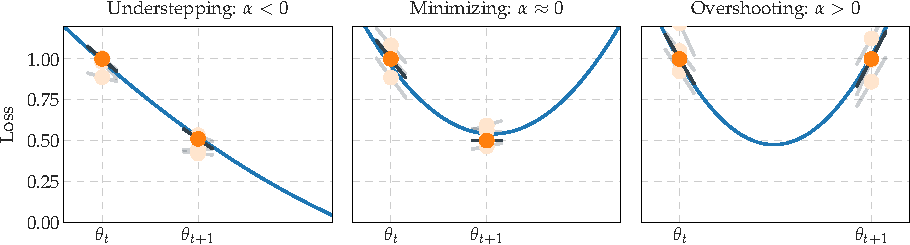
\includegraphics[width =
  \linewidth]{../repos/cockpit-paper/fig/12_alpha_explanation/output/alpha_explanation_thesis-wide}
  \caption{\textbf{Motivational sketch for the $\alpha$ quantity.} In each
    iteration of the optimizer we observe the loss function at two positions
    $\vtheta_{t}$ and $\vtheta_{t+1}$ (shown in
    \textcolor{sns_orange}{\ding{108}}). The black lines
    (\textcolor{TUdark}{\textbf{---}}) show the observed slope at this position,
    which we can get from projecting the gradients onto the current step
    direction $\vtheta_{t+1} - \vtheta_{t}$. Note, that all four observations
    (two loss and two slope values) are noisy, due to being computed on a
    mini-batch. With access to the individual losses and gradients (some samples
    shown in
    \textcolor{sns_orange_light}{\ding{108}}/\textcolor{TUgray}{\textbf{---}}),
    we can estimate their noise level and build a noise-informed quadratic fit
    (\textcolor{sns_blue}{\textbf{---}}). Using this fit, we determine whether
    the optimizer minimizes the local uni-variate loss (\textit{middle plot}), or
    whether we understep (\textit{left plot}) or overshoot (\textit{right plot})
    the minimum.}
  \label{cockpit::fig:alpha_explanation}
\end{figure*}

\subsubsection{Motivation}

The goal of the $\alpha$-quantity is to estimate and quantify the effect that a
selected learning rate has on the optimizer's steps. Consider the optimizer's
step at training iteration $t$. This parameter update from $\vtheta_{t}$ to
$\vtheta_{t+1}$ happens in a one-dimensional space, defined by the update
direction $\vtheta_{t+1} - \vtheta_{t}=\vs_t$. The update direction depends on
the update rule of the optimizer, \eg for \sgd with learning rate $\eta$ it is
simply $\vs_t =- \eta \vg_{\sB_t}(\vtheta_{t})$.

We build a noise-informed uni-variate quadratic approximation along this update
step ($\vtheta_{t} \to \vtheta_{t+1}$) based on the two noisy loss function
observations at $\vtheta_{t}$ and $\vtheta_{t+1}$ and the two noisy slope
observation at these two points. Examining this quadratic fit, we are able to
determine where on this parabola our optimizer steps. Standardizing this, we
express a step to the minimum of the loss in the update direction as $\alpha=0$.
Analogously, steps that end short of this minimum result in $\alpha<0$, and a
step over the minimum in $\alpha>0$. These three different scenarios are
illustrated in \Cref{cockpit::fig:alpha_explanation} also showing the underlying
observations that would lead to them. \Cref{cockpit::fig:LINE} shows the distribution of
$\alpha$-values for two very different optimization trajectories.

\subsubsection{Noisy Observations}

In order to build an approximation for the loss function in the update
direction, we leverage the four observations of the function (and its
derivative) that are available in each iteration. Due to the stochasticity of
deep learning optimization, we also take into account the noise-level of all
observations by estimating them. The first two observations are the mini-batch
training losses $\mathcal{L}_{\sB_t}(\vtheta_t),
\mathcal{L}_{\sB_{t+1}}(\vtheta_{t+1})$ at point $\vtheta_{t}$ and
$\vtheta_{t+1}$, which are computed in every standard training loop. The
mini-batch losses are averages over individual losses,
\begin{align*}
  \mathcal{L}_{\sB_t}(\vtheta_t)
  &=
    \E_{\sB_t}\left[ \ell(\vtheta_t) \right] = \frac{1}{|\sB_t|} \sum_{n \in \sB_t}
    \ell_n(\vtheta_t) \,,
  \\
  \mathcal{L}_{\sB_{t+1}}(\vtheta_{t+1})
  &=
    \E_{\sB_{t+1}}\left[ \ell(\vtheta_{t+1}) \right] = \frac{1}{|\sB_{t+1}|} \sum_{n \in \sB_{t+1}}
    \ell_n(\vtheta_{t+1})\,,
\end{align*}
and using these individual losses, we can also compute the variances to estimate
the noise-level of our loss observation,
\begin{align*}
  \Var_{\sB_{t}} \left[ \ell(\vtheta_t) \right]
  =&
     \left( \frac{1}{|\sB_t|} \sum_{n \in \sB_t} \ell_n(\vtheta_t)^2 \right)
     -
     \left( \frac{1}{|\sB_t|} \sum_{n \in \sB_t} \ell_n(\vtheta_t) \right)^2 \, ,
  \\
  \Var_{\sB_{t+1}} \left[ \ell(\vtheta_{t+1}) \right]
  =&
     \left( \frac{1}{|\sB_{t+1}|} \sum_{n \in \sB_{t+1}} \ell_n(\vtheta_{t+1})^2 \right)
     -
     \left( \frac{1}{|\sB_{t+1}|} \sum_{n \in \sB_{t+1}} \ell_n(\vtheta_{t+1}) \right)^2 \, .
\end{align*}
Similarly, we proceed with the slope in the update direction. To compute the
slope of the loss function in the direction of the optimizer's update $\vs_t$,
we project the current gradient along this update direction
\begin{align*}
  \E_{\sB_t} \left[\frac{\vs_t^\top \vg(\vtheta_t)}{\lVert \vs_t
  \rVert^2}\right]
  =&
     \frac{1}{|\sB_{t}|} \sum_{n\in \sB_t} \frac{\vs_t^\top \vg_n(\vtheta_t)}{\lVert
     \vs_t \rVert^2} \, ,
  \\
  \E_{\sB_{t+1}} \left[\frac{\vs_t^\top \vg(\vtheta_{t+1})}{\lVert \vs_t
  \rVert^2}\right]
  =&
     \frac{1}{|\sB_{t+1}|} \sum_{n\in \sB_{t+1}} \frac{\vs_t^\top \vg_n(\vtheta_{t+1})}{\lVert
     \vs_t \rVert^2} \, .
\end{align*}
Just like before, we can also compute the variance of this slope, by leveraging
individual gradients,
\begin{align*}
  &\Var_{\sB_t} \left[\frac{\vs_t^\top \vg(\vtheta_t)}{\lVert \vs_t
  \rVert^2}\right]
    \\
  &\quad=
     \frac{1}{|\sB_t|} \sum_{n\in B_t} \left( \frac{\vs_t^\top \vg_n(\vtheta_t)}{\lVert
     \vs_t \rVert^2} \right)^2
     -  \left( \frac{1}{|\sB_t|} \sum_{n\in \sB_t} \frac{\vs_t^\top
     \vg_n(\vtheta_t)}{\lVert \vs_t \rVert^2} \right)^2 \, ,
  \\
  &\Var_{\sB_{t+1}} \left[\frac{\vs_t^\top \vg(\vtheta_{t+1})}{\lVert \vs_t
  \rVert^2}\right]
    \\
  &\quad=
     \frac{1}{|\sB_{t+1}|} \sum_{n\in \sB_{t+1}} \left( \frac{\vs_t^\top \vg_n(\vtheta_{t+1})}{\lVert
     \vs_t \rVert^2} \right)^2
     -  \left( \frac{1}{|\sB_{t+1}|} \sum_{n\in \sB_{t+1}} \frac{\vs_t^\top
     \vg_n(\vtheta_{t+1})}{\lVert \vs_t \rVert^2} \right)^2 \, .
\end{align*}

\subsubsection{Quadratic Fit \& Normalization}

Using our (noisy) observations, we are now ready to build an approximation for
the loss as a function of the step size, which we will denote as $f(\tau)$. We
assume a quadratic function for $f$, which follows recent reports for the loss
landscape of neural networks \citep{xing2018walk}, \ie a function $f(\tau) = w_0
+ w_1 \tau + w_2 \tau^2$ parameterized by $\vw \in \R^3$. We further assume a
Gaussian likelihood of the form
\begin{align}
  \label{cockpit::eq:alpha_likelihood}
  p\left(\giventhat{\tilde{\vf}}{\vw, \mPhi}\right)
  =
  \mathcal{N}\left(\giventhat{\tilde{\vf}}{ \mPhi^\top \vw, \mLambda}\right)
\end{align}
for observations $\tilde{\vf}$ of the loss and its slope. The observation matrix
$\mPhi$ and the noise matrix of the observations $\mLambda$ are
\begin{align*}
  \mPhi = \begin{pmatrix}
    1 & 1 & 0 & 0 \\
    \tau_1 & \tau_2  & 1 & 1 \\
    \tau_1^2 & \tau_2^2 & 2\tau_1 &  2\tau_2
  \end{pmatrix}\,,
                                    \qquad \qquad
                                    \mLambda = \begin{pmatrix}
                                      \sigma_{\tilde{f}_1} & 0 & 0 & 0 \\ 0 & \sigma_{\tilde{f}_2} & 0 & 0  \\ 0
                                      & 0 & \sigma_{\tilde{f}'_1} & 0 \\ 0 & 0 & 0 & \sigma_{\tilde{f}'_2}
                                    \end{pmatrix} \, ,
\end{align*}
where $\tau$ denotes the position and $\sigma$ denotes the noise-level estimate
of the observation. The maximum likelihood solution of
\Cref{cockpit::eq:alpha_likelihood} for the parameters of our quadratic fit is given by
\begin{align}
  \label{cockpit::eq:alpha-feature-table}
  \vw = \left(\mPhi \mLambda^{-1}\mPhi^\top\right)^{-1}\mPhi \mLambda^{-1}
  \tilde{\vf} \, .
\end{align}
Once we have the quadratic fit of the uni-variate loss along the update
direction, we normalize the scales such that the resulting $\alpha$ expresses
the effective step taken by the optimizer sketched in
\Cref{cockpit::fig:alpha_explanation}.

\subsubsection{Usage}

The $\alpha$-quantity is related to recent line search approaches
\cite{mahsereci2017probabilistic,vaswani2019painless}. However, instead of searching for an
acceptable step by repeated attempts, we instead report the effect of the
current step size selection. This could, for example, be used to disentangle the
two optimization runs in \Cref{cockpit::fig:LINE}. Additionally, this information could
also be used to automatically adapt the learning rate during the training
process. But, as discussed in \Cref{cockpit::sec:alpha_exp}, it isn't trivial what the
``correct'' decision is, as it might depend on the optimization problem, the
training phase, and other factors. Having this $\alpha$-quantity can, however,
provide more insight into what kind of steps are used in well-tuned runs with
traditional optimizers such as \sgd.

%%% Local Variables:
%%% mode: latex
%%% TeX-master: "../thesis"
%%% End:

\subsection{\cabs Criterion: Coupling Adaptive Batch Sizes with Learning Rates
  (\robustInlinecode{CABS})}\label{cockpit::app:cabs}

The \cabs criterion, proposed by \citet{balles2017coupling}, can be used to adapt the
mini-batch size during training with \sgd. It relies on the gradient noise and
approximately optimizes the objective's expected gain per cost. The adaptation
rule is (with learning rate $\eta$)
\begin{equation}
  \label{cockpit::eq:cabs-theoretical}
  |\sB| \leftarrow \eta \frac{\Tr(\mSigma_{\pdata}(\vtheta))}{\gL_{{\pdata}}(\vtheta)}\,,
\end{equation}
and the practical implementation approximates $ \gL_{{\pdata}}(\vtheta) \approx
\gL_{\sB}(\vtheta)$and $\Tr(\mSigma_{\pdata}(\vtheta)) \approx
\nicefrac{(|\sB|-1)}{|\sB|} \Tr(\hat{\mSigma}_\sB(\vtheta))$ (compare equations
(10, 22) and first paragraph of Section 4 in \citep{balles2017coupling}). This
yields the quantity computed in \cockpit's \inlinecode{CABS} instrument,
\begin{align}
  \label{cockpit::eq:cabs-feature-table}
  |\sB| &\leftarrow \eta \frac{
          \frac{1}{|\sB|}
          \sum_{j=1}^D \sum_{n\in\sB}
          \left[
          \vg_n(\vtheta) - \vg_{\sB}(\vtheta)
          \right]_j^2
          }{
          \gL_{\sB}(\vtheta)
          }\,.
\end{align}

\subsubsection{Usage}

The \cabs criterion suggests a batch size which is optimal
under certain assumptions. This suggestion can support practitioners in the
batch size selection for their deep learning task.

%%% Local Variables:
%%% mode: latex
%%% TeX-master: "../thesis"
%%% End:

\subsection{Early-stopping Criterion for SGD
  (\robustInlinecode{EarlyStopping})}\label{cockpit::app:early-stopping}

The empirical risk $\gL_{\sD}(\vtheta)$, and the mini-batch loss
$\gL_{\sB}(\vtheta)$ are only estimators of the target objective
$\gL_{\pdata}(\vtheta)$. \citet{mahsereci2017early} motivate
$p(\giventhat{\vg_{\sB,\sD}(\vtheta)}{\vg_{\pdata}(\vtheta) = \vzero})$ as a measure for
detecting noise in the finite datasets $\sB, \sD$ due to sampling from $\pdata$.
They propose an evidence-based (EB) criterion for early stopping the training
procedure based on mini-batch statistics, and model $p(\vg_{\sB}(\vtheta))$ with
a sampled diagonal variance approximation (compare
\Cref{cockpit::eq:cheat-sheet-risk-gradient-diagonal-variance-estimator}),
\begin{equation}
  p(\vg_{\sB}(\vtheta))
  \approx \prod_{j=1}^D  \gN\left(
    \giventhat{
      \vg_{\sB}(\vtheta)
    }{
      \left[\vg_{\pdata}(\vtheta)\right]_j,
      \frac{\left[ \hat{\mSigma}_\sB(\vtheta)\right]_{j,j}}{|\sB|}
    }
  \right)\,.
\end{equation}
Their \sgd stopping criterion is
\begin{subequations}
  \begin{align}
    \frac{2}{D} \left[ \log p(\vg_{\sB}(\vtheta))
    - \E_{\vg_{\sB}(\vtheta) \sim p(\vg_{\sB}(\vtheta))} \left[ \log p(\vg_{\sB}(\vtheta))\right]
    \right]
    &> 0\,,
      \intertext{and translates into}
      1 - \frac{|\sB|}{D} \sum_{d=1}^D \frac{
      \left[ \vg_{\sB}(\vtheta)\right]_d^2
      }{
      \left[ \hat{\mSigma}_\sB(\vtheta)\right]_{d,d}
      }
    &> 0\,,
    \\
    1 - \frac{|\sB|}{D} \sum_{d=1}^D \frac{
    \left[ \vg_{\sB}(\vtheta)\right]_d^2
    }{
    \frac{1}{|\sB| - 1}
    \sum_{n\in \sB}
    \left[
    \vg_n(\vtheta) - \vg_{\sB}(\vtheta)
    \right]_d^2
    }
    &> 0\,,
    \\
    \label{cockpit::eq:early-stopping-feature-table}
    1 - \frac{|\sB| (|\sB| - 1)}{D} \sum_{d=1}^D \frac{
    \left[ \vg_{\sB}(\vtheta)\right]_d^2
    }{
    \left(
    \sum_{n\in \sB}
    \left[
    \vg_n(\vtheta)
    \right]_d^2
    \right)
    - |\sB|
    \left[
    \vg_{\sB}(\vtheta)
    \right]_d^2
    }
    &> 0\,.
  \end{align}
\end{subequations}
\cockpit's \inlinecode{EarlyStopping} quantity computes the left side of
\Cref{cockpit::eq:early-stopping-feature-table}.

\subsubsection{Usage}

\cockpit's \inlinecode{EarlyStopping} quantity can inform practitioners that
training is about to be completed and the model might be at risk of overfitting.

%%% Local Variables:
%%% mode: latex
%%% TeX-master: "../thesis"
%%% End:

\subsection{Individual Gradient Element Histograms (\robustInlinecode{GradHist1d},
  \robustInlinecode{GradHist2d})}
For the $|\sB| \times D$ individual gradient elements, \cockpit's
\inlinecode{GradHist1d} instrument displays a histogram of
\begin{equation}
  \label{cockpit::eq:app-grad-hist-1d}
  \left\{
    [\vg_n(\vtheta)]_d
  \right\}_{n\in\sB,d=1,\dots, D}\,.
\end{equation}
\cockpit's \inlinecode{GradHist2d} instrument displays a two-dimensional histogram
of the $|\sB| \times D$ tuples
\begin{equation}
  \label{cockpit::eq:app-grad-hist-2d}
  \left\{
    \left(
      [\vtheta]_d,
      [\vg_n(\vtheta)]_d
    \right)
  \right\}_{n\in\sB,d=1,\dots, D}\,
\end{equation}
and the marginalized one-dimensional histograms over the parameter and gradient
axes.

\subsubsection{Usage}

\Cref{cockpit::sec:misscaled_data_exp,cockpit::sec:vanishing_gradient_exp}
provide use cases (identifying data pre-processing issues and vanishing
gradients) for both the gradient histogram as well as its layer-wise extension.

%%% Local Variables:
%%% mode: latex
%%% TeX-master: "../thesis"
%%% End:

\subsection{Gradient Tests (\robustInlinecode{NormTest},
  \robustInlinecode{InnerTest},
  \robustInlinecode{OrthoTest})}\label{cockpit::app:gradient_tests}

\citet{bollapragada2017adaptive} and \citet{byrd2012sample} propose batch size adaptation
schemes based on the gradient noise. They formulate geometric constraints
between population and mini-batch gradient and accessible approximations that
can be probed to decide whether the mini-batch size should be increased. Because
mini-batches are \iid from $\pdata$, it holds that
\begin{subequations}
  \label{cockpit::eq:iid-sampling-expectation}
  \begin{align}
    \E\left[\vg_{\sB}(\vtheta) \right]
    &=
      \vg_{\pdata}(\vtheta),
    \\
    \E\left[ \vg_{\sB}(\vtheta)^\top \vg_{\pdata}(\vtheta)  \right]
    &=
      \lVert \vg_{\pdata}(\vtheta)  \rVert^2.
  \end{align}
\end{subequations}

The above works propose enforcing other weaker similarity in expectation during
optimization. These geometric constraints reduce to basic vector geometry (see
\Cref{cockpit::subfig:gradient-test-sketch1} for an overview of the relevant
vectors). We recall their formulation here for consistency and derive the
practical versions, which can be computed from training observables and are used
in \cockpit (consult \Cref{cockpit::subfig:gradient-test-sketch2} for the
visualization).

\begin{figure*}[ht]
  \centering
  \begin{subfigure}[t]{0.59\linewidth}
    \centering
    \tikzexternalenable
    \begin{tikzpicture}[rotate=5, >=latex, very thick, xscale = 1., yscale =
      1.25]

      % node style
      \tikzset{my label style/.style={fill=white, fill opacity=0.5, text
          opacity=1, font=\footnotesize}}


      % expected risk gradient
      \draw[->, ultra thick] (0,0) to node [midway, anchor=north west, my label
      style] {$\vg_{\pdata}$} (7,0);

      % mini-batch gradient
      \draw[->] (0,0) to node [midway, anchor=south east, my label style]
      {$\vg_{\sB}$} (6,3);
      \draw[->, >=latex] (0,0) -- (6,3);

      % right angle
      % \draw (6,0) rectangle ++(-0.15,0.15);

      % residual
      \draw[->, sns_blue] (7,0) to node [midway, right, anchor=south west, my label
      style] {$\vg_{\sB} - \vg_{\pdata}$} (6,3);

      % projection
      \draw[->, sns_orange] (0,0) to node [midway, above, anchor=south east, my label
      style] {$\mathrm{proj}_{\vg_{\pdata}}\left(\vg_{\sB}\right)$} (6,0);

      % orthogonal residual
      \draw[->, sns_green] (6,0) to node [midway, left, anchor=north east, my label
      style] {$\vg_{\sB} - \mathrm{proj}_{\vg_{\pdata}}\left(\vg_{\sB}\right)$} (6,3);
    \end{tikzpicture}
    \tikzexternaldisable
    \caption{Relevant vectors}
    \label{cockpit::subfig:gradient-test-sketch1}
  \end{subfigure}
  \begin{subfigure}[t]{0.39\linewidth}
    \centering
    \tikzexternalenable
    \begin{tikzpicture}[>=latex, very thick, xscale = 2, yscale = 2]
      \clip (-1,0) rectangle (1,2);

      % expected risk gradient
      % \draw[->, ultra thick] (0,0) to (0,1);
      % target indicator
      \draw[ultra thick] (0,0.9) to (0,1.1);
      \draw[ultra thick] (-0.1,1) to (0.1,1);

      % norm test
      \pgfmathsetmacro{\normTestRadius}{0.5}
      \filldraw [fill=sns_blue, opacity=0.4] (0,1) circle (\normTestRadius);

      % inner product test
      \pgfmathsetmacro{\innerProductWidth}{0.2}
      \filldraw [fill=sns_orange, opacity=0.4] (-2,1 - \innerProductWidth) rectangle
      (2,1 + \innerProductWidth);

      % orthogonality test
      \pgfmathsetmacro{\orthogonalityTestWidth}{0.3}
      \filldraw [fill=sns_green, opacity=0.4] (-\orthogonalityTestWidth, 0) rectangle
      (\orthogonalityTestWidth, 2);

      % norm test label
      \draw[ultra thick, <->, sns_blue] (0,1) to ++(45:\normTestRadius) node [above, right] {\footnotesize $\theta_{\text{norm}}$};

      % inner product test label
      \draw[ultra thick, <->, sns_orange] (-0.75, 1 - \innerProductWidth) to ++(0, 2 *\innerProductWidth) node [above] {\footnotesize $2 \theta_{\text{inner}}$};

      % orthogonality test label
      \draw[ultra thick, <->, sns_green] (-\orthogonalityTestWidth0, 0.2) to ++(2 *\orthogonalityTestWidth, 0.) node [right] {\footnotesize $2 \nu_{\text{ortho}}$};

      % acute angle test
      % \pgfmathsetmacro{\acuteAngle}{30}
      % \pgfmathsetmacro{\initAngle}{90 - \acuteAngle}
      % \pgfmathsetmacro{\endAngle}{90 + \acuteAngle}
      % \pgfmathsetmacro{\acuteAngleRadius}{3}

      % \filldraw [fill=black, opacity=0.2] (0,0) --
      % (\initAngle:\acuteAngleRadius) arc
      % (\initAngle:\endAngle:\acuteAngleRadius) -- cycle;
    \end{tikzpicture}
    \tikzexternaldisable
    \caption{\cockpit's gradient test visualization.}
    \label{cockpit::subfig:gradient-test-sketch2}
  \end{subfigure}
  \caption{\textbf{Conceptual sketch for gradient tests.}
    \subfigref{cockpit::subfig:gradient-test-sketch1} Relevant vectors to
    formulate the geometric constraints between population and mini-batch
    gradient probed by the gradient tests.
    \subfigref{cockpit::subfig:gradient-test-sketch2} Gradient test
    visualization in \cockpit.}
  \label{cockpit::fig:gradient-tests-sketch}
\end{figure*}

\subsubsection{Usage}

All three gradient tests describe the noise level of the gradients.
\citet{bollapragada2017adaptive} and \citet{byrd2012sample} adapt the batch size
so that the proposed geometric constraints are fulfilled. Practitioners can use
the combined gradient test plot, \ie top center plot in
\Cref{cockpit::fig:showcase}, to monitor gradient noise during training and
adjust hyperparameters such as the batch size.


\subsubsection{Norm Test (\robustInlinecode{NormTest})}\label{cockpit::app:norm-test}
The norm test \citep{byrd2012sample} constrains the residual norm $\lVert
\vg_{\sB}(\vtheta) - \vg_{\pdata}(\vtheta) \rVert$, rescaled by $\lVert
\vg_{\pdata}(\vtheta) \rVert$. This gives rise to a standardized ball of radius
$\theta_{\text{norm}} \in (0, \infty)$ around the population gradient, where the
mini-batch gradient should reside. \citet{byrd2012sample} set
$\theta_{\text{norm}} = 0.9$ in their experiments and increase the batch size if
(in the practical version, see below) the following constraint is not fulfilled
\begin{subequations}
  \begin{align}
    \label{cockpit::eq:norm-test-constraint}
    \E\left[ \frac{ \left\lVert \vg_{\sB}(\vtheta) - \vg_{\pdata}(\vtheta)
    \right\rVert^2 }{\left\lVert \vg_{\pdata}(\vtheta) \right\rVert^2} \right]
    \le
    \theta_{\text{norm}}^2\,.
  \end{align}
  Instead of taking the expectation over mini-batches, \citet{byrd2012sample} note
  that the above will be satisfied if
  \begin{equation}
    \label{cockpit::eq:norm-test-individual}
    \frac{1}{|\sB|} \E\left[ \frac{ \left\lVert \vg_n(\vtheta) - \vg_{\pdata}(\vtheta)
        \right\rVert^2 }{\left\lVert \vg_{\pdata}(\vtheta) \right\rVert^2} \right]
    \le \theta_{\text{norm}}^2\,.
  \end{equation}
\end{subequations}
They propose a practical form of this test,
\begin{subequations}
  \begin{equation}
    \label{cockpit::eq:norm-test-practical-proposed}
    \frac{1}{|\sB| (|\sB| - 1)} \frac{\sum_{n \in \sB} \left\lVert \vg_n(\vtheta) -
        \vg_{\sB}(\vtheta) \right\rVert^2}{\left\lVert
        \vg_{\sB}(\vtheta)\right\rVert^2} \le \theta_{\text{norm}}^2\,,
  \end{equation}
  which can be computed from mini-batch statistics. Rearranging
  \begin{align}
    \sum_{n \in \sB} \left\lVert \vg_n(\vtheta) - \vg_{\sB}(\vtheta) \right\rVert^2
    &= \left( \sum_{n \in \sB} \left\lVert \vg_n(\vtheta) \right\rVert^2 \right) - |\sB|
      \left\lVert \vg_{\sB}(\vtheta) \right\rVert^2\,,
  \end{align}
  we arrive at
  \begin{align}
    \label{cockpit::eq:norm-test-feature-table}
    \frac{1}{|\sB| (|\sB| - 1)} \left[ \frac{ \sum_{n \in \sB} \left\lVert
    \vg_n(\vtheta) \right\rVert^2 }{\left\lVert
    \vg_{\sB}(\vtheta)\right\rVert^2} - |\sB| \right] &\le
                                                        \theta_{\text{norm}}^2
  \end{align}
\end{subequations}
that leverages the norm of both the mini-batch and the individual gradients,
which can be aggregated over parameters during a backward pass. \cockpit's
\inlinecode{NormTest} corresponds to the maximum radius $\theta_{\text{norm}}$
for which the above inequality holds.

\subsubsection{Inner Product Test
  (\robustInlinecode{InnerTest})}\label{cockpit::app:inner-product-test}
The inner product test \citep{bollapragada2017adaptive} constrains the
projection of $\vg_{\sB}(\vtheta)$ onto $\vg_{\pdata}(\vtheta)$ (compare
\Cref{cockpit::subfig:gradient-test-sketch1}),
\begin{align}
  \label{cockpit::eq:inner-product-projection}
  \mathrm{proj}_{\vg_{\pdata}(\vtheta)}\left(\vg_{\sB}(\vtheta)\right)
  :=
  \frac{\vg_{\sB}(\vtheta)^\top \vg_{\pdata}(\vtheta)}{\left\lVert
  \vg_{\pdata}(\vtheta) \right\rVert^2} \vg_{\pdata}(\vtheta)\,,
\end{align}
rescaled by $\lVert \vg_{\pdata}(\vtheta) \rVert$. This restricts the mini-batch
gradient to reside in a standardized band of relative width
$\theta_{\text{inner}}\in (0, \infty)$ around the population risk gradient.
\citet{bollapragada2017adaptive} use $\theta_{\text{inner}} = 0.9$ (in the practical
version, see below) to adapt the batch size if the parallel component's variance
does not satisfy the condition
\begin{subequations}
  \begin{align}
    \label{cockpit::eq:inner-product-test}
    \Var\left( \frac{\vg_{\sB}(\vtheta)^\top \vg_{\pdata}(\vtheta)}{\left\lVert
    \vg_{\pdata}(\vtheta) \right\rVert^2} \right)
    &= \E\left[ \left( \frac{\vg_{\sB}(\vtheta)^\top \vg_{\pdata}(\vtheta)}{\left\lVert
      \vg_{\pdata}(\vtheta) \right\rVert^2}  -1 \right)^2 \right]
      \le \theta_{\text{inner}}^2
  \end{align}
  (note that by \Cref{cockpit::eq:iid-sampling-expectation} we have $\E[
    \nicefrac{\vg_{\sB}(\vtheta)^\top \vg_{\pdata}(\vtheta)}{\left\lVert \vg_{\pdata}(\vtheta)
      \right\rVert^2} ] = 1 $). \citet{bollapragada2017adaptive} bound
  \Cref{cockpit::eq:inner-product-test} by the individual gradient variance,
  \begin{align}
    \label{cockpit::eq:inner-product-test-individual}
    \begin{split}
      &\frac{1}{|\sB|}\Var\left( \frac{\vg_n(\vtheta)^\top \vg_{\pdata}(\vtheta)}{\left\lVert
      \vg_{\pdata}(\vtheta) \right\rVert^2}\right)
      \\
      &\qquad =
      \frac{1}{|\sB|} \E \left[ \left( \frac{\vg_n(\vtheta)^\top \vg_{\pdata}(\vtheta) }{\left\lVert
      \vg_{\pdata}(\vtheta) \right\rVert^2} - 1    \right)^2  \right] \le \theta_{\text{inner}}^2\,.
    \end{split}
  \end{align}
\end{subequations}
They then propose a practical form of \Cref{cockpit::eq:inner-product-test-individual},
which uses the mini-batch sample variance,
\begin{subequations}
  \begin{align}
    \label{cockpit::eq:inner-product-test-practical}
    \begin{split}
    &\frac{1}{|\sB|} \Var\left( \frac{\vg_n(\vtheta)^\top \vg_{\sB}(\vtheta)}{\left\lVert
    \vg_{\sB}(\vtheta)\right\rVert^2}\right)
      \\
      &\qquad
    = \frac{1}{|\sB| (|\sB| - 1)}\left[  \sum_{n\in \sB}  \left( \frac{\vg_n(\vtheta)^\top \vg_{\sB}(\vtheta)}{\left\lVert
    \vg_{\sB}(\vtheta)\right\rVert^2} - 1    \right)^2  \right]
    \le \theta_{\text{inner}}^2\,.
    \end{split}
  \end{align}
  Expanding
  \begin{align}
    \label{cockpit::eq:inner-product-test-practical-rewrite}
    \sum_{n\in \sB}  \left( \frac{\vg_n(\vtheta)^\top \vg_{\sB}(\vtheta)}{\left\lVert
    \vg_{\sB}(\vtheta)\right\rVert^2} - 1    \right)^2
    &=
      \frac{\sum_{n\in \sB}  \left( \vg_n(\vtheta)^\top \vg_{\sB}(\vtheta)\right)^2}{\left\lVert
      \vg_{\sB}(\vtheta)\right\rVert^4} - |\sB|
  \end{align}
  and inserting \Cref{cockpit::eq:inner-product-test-practical-rewrite} into
  \Cref{cockpit::eq:inner-product-test-practical} yields
  \begin{align}
    \label{cockpit::eq:inner-product-test-feature-table}
    \frac{1}{|\sB| (|\sB| - 1)}
    \left[   \frac{\sum_{n\in \sB}  \left( \vg_n(\vtheta)^\top \vg_{\sB}(\vtheta)\right)^2}{\left\lVert
    \vg_{\sB}(\vtheta)\right\rVert^4} - |\sB|\right]
    &\le \theta_{\text{inner}}^2\,.
  \end{align}
\end{subequations}
It relies on pairwise scalar products between individual gradients, which can be
aggregated over layers during backpropagation. \cockpit's \inlinecode{InnerTest}
quantity computes the maximum band width $\theta_{\text{inner}}$ that satisfies
\Cref{cockpit::eq:inner-product-test-feature-table}.

\subsubsection{Orthogonality Test (\robustInlinecode{OrthoTest})}\label{cockpit::app:orthogonality-test}
In contrast to the inner product test (\Cref{cockpit::app:inner-product-test})
which constrains the projection (\Cref{cockpit::eq:inner-product-projection}),
the orthogonality test \citep{bollapragada2017adaptive} constrains the
orthogonal part (see \Cref{cockpit::fig:gradient-tests-sketch} (a))
\begin{align}
  \label{cockpit::eq:orthogonality-projection}
  \vg_{\sB}(\vtheta)
  -
  \mathrm{proj}_{\vg_{\pdata}(\vtheta)}\left(\vg_{\sB}(\vtheta)\right)\,,
\end{align}
rescaled by $\lVert \vg_{\pdata}(\vtheta) \rVert$. This restricts the mini-batch
gradient to a standardized band of relative width $\nu_{\text{ortho}} \in (0,
\infty)$ parallel to the population gradient. \citet{bollapragada2017adaptive} use $\nu
= \tan(80^{\circ}) \approx 5.84$ (in the practical version, see below) to adapt
the batch size if the following condition is violated,
\begin{subequations}
  \begin{align}
    \label{cockpit::eq:orthogonality-test-constraint}
    \E\left[
    \left\lVert
    \frac{
    \vg_{\sB}(\vtheta)
    -
    \mathrm{proj}_{\vg_{\pdata}(\vtheta)}\left(\vg_{\sB}(\vtheta)\right)
    }{
    \lVert \vg_{\pdata}(\vtheta) \rVert
    }
    \right\rVert^2
    \right]
    \le \nu^2_{\text{ortho}}\,.
  \end{align}
  Expanding the norm, and inserting \Cref{cockpit::eq:inner-product-projection}, this
  simplifies to
  \begin{align}
    \begin{split}
      \E \left[ \left\lVert \frac{ \vg_{\sB}(\vtheta) }{ \lVert \vg_{\pdata}(\vtheta)
      \rVert } - \frac{ \vg_{\sB}(\vtheta)^\top \vg_{\pdata}(\vtheta) }{ \lVert
      \vg_{\pdata}(\vtheta) \rVert^2 } \frac{ \vg_{\pdata}(\vtheta) }{ \lVert
      \vg_{\pdata}(\vtheta) \rVert} \right\rVert^2 \right] &\le
                                                        \nu^2_{\text{ortho}}\,,
      \\
      \E\left[ \frac{ \lVert \vg_{\sB}(\vtheta) \rVert^2 }{ \lVert
      \vg_{\pdata}(\vtheta) \rVert^2 } - \frac{ \left( \vg_{\sB}(\vtheta)^\top
      \vg_{\pdata}(\vtheta) \right)^2 }{ \lVert \vg_{\pdata}(\vtheta) \rVert^4 }
      \right] &\le \nu^2_{\text{ortho}}\,.
    \end{split}
  \end{align}
  \citet{bollapragada2017adaptive} bound this inequality with individual gradients,
  \begin{align}
    \frac{1}{|\sB|}
    \E \left[
    \left\lVert
    \frac{
    \vg_n(\vtheta)
    }{
    \lVert
    \vg_{\pdata}(\vtheta)
    \rVert^2
    }
    -
    \frac{
    \vg_n(\vtheta)^\top
    \vg_{\pdata}(\vtheta)
    }{
    \lVert
    \vg_{\pdata}(\vtheta)
    \rVert^2
    }
    \frac{
    \vg_{\pdata}(\vtheta)
    }{
    \left\lVert
    \vg_{\pdata}(\vtheta)
    \right\rVert}
    \right\rVert^2
    \right]
    &\le \nu^2_{\text{ortho}}\,.
  \end{align}
\end{subequations}
They propose the practical form
\begin{subequations}
  \begin{align}
    \frac{1}{|\sB|(|\sB|-1)}
    \E\left[
    \left\lVert
    \frac{
    \vg_n(\vtheta)
    }{
    \lVert
    \vg_{\sB}(\vtheta)
    \rVert
    }
    -
    \frac{
    \vg_n(\vtheta)^\top
    \vg_{\sB}(\vtheta)
    }{
    \lVert
    \vg_{\sB}(\vtheta)
    \rVert^2
    }
    \frac{
    \vg_{\sB}(\vtheta)
    }{
    \left\lVert
    \vg_{\sB}(\vtheta)
    \right\rVert}
    \right\rVert^2
    \right]
    &\le \nu^2_{\text{ortho}}\,,
  \end{align}
  which simplifies to
  \begin{align}
    \label{cockpit::eq:orthogonality-test-feature-table}
    \frac{1}{|\sB| (|\sB| - 1)}
    \sum_{n \in \sB }
    \left(
    \frac{
    \lVert
    \vg_n(\vtheta)
    \rVert^2
    }{
    \lVert
    \vg_{\sB}(\vtheta)
    \rVert^2
    }
    -
    \frac{
    \left(
    \vg_n(\vtheta)^\top
    \vg_{\sB}(\vtheta)
    \right)^2
    }{
    \lVert
    \vg_{\sB}(\vtheta)
    \rVert^4
    }
    \right)
    &\le \nu^2_{\text{ortho}}\,.
  \end{align}
\end{subequations}
It relies on pairwise scalar products between individual gradients which can be
aggregated over layers during a backward pass. \cockpit's \inlinecode{OrthoTest}
quantity computes the maximum band width $\nu_{\text{ortho}}$ which satisfies
\Cref{cockpit::eq:orthogonality-test-feature-table}.

\subsubsection{Relation to Acute Angle Test}

Recently, a novel ``acute angle test'' was proposed by
\citet{bahamou2019dynamic}. While the theoretical constraint between
$\vg_{\sB}(\vtheta)$ and $\vg_{\pdata}(\vtheta)$ differs from the orthogonality
test, the practical versions coincide. Hence, we do not incorporate the acute
angle here.

%%% Local Variables:
%%% mode: latex
%%% TeX-master: "../thesis"
%%% End:

\subsection{Hessian Maximum Eigenvalue
  (\robustInlinecode{HessMaxEV})}\label{cockpit::app:max-ev}

The Hessian's maximum eigenvalue $\lambda_{\text{max}}(\mH_{\sB}(\vtheta))$ is
computed with an iterative eigensolver from Hessian-vector products through
\pytorch's automatic differentiation \citep{pearlmutter1994fast}. Like
\citet{yao2020pyhessian}, we employ power iterations with similar
\href{https://github.com/amirgholami/PyHessian/blob/0f7e0f63a0f132998608013351ba19955fc9d861/pyhessian/hessian.py#L111-L158}{default
  stopping parameters} (stop after at most 100 iterations, or if the iterate
does converged with a relative and absolute tolerance of $10^{-3}, 10^{-6}$,
respectively) to compute $\lambda_{\text{max}}(\mH_{\sB}(\vtheta))$ through the
\inlinecode{HessMaxEV} quantity in \cockpit.

In principle, more sophisticated eigensolvers (for example Arnoldi's method)
could be applied to converge in fewer iterations or compute eigenvalues other
than the leading ones. \citet{warsa2004krylov} empirically demonstrate that the
FLOP ratio between power iteration and implicitly restarted Arnoldi method can
reach values larger than $100$. While we can use such a beneficial method on a
CPU through
\href{https://docs.scipy.org/doc/scipy/reference/generated/scipy.sparse.linalg.eigsh.html} {\texttt{scipy.sparse.linalg.eigsh}}
we are restricted to the GPU-compatible power iteration for GPU training. We
expect that extending the support of popular machine learning libraries like
\pytorch for such iterative eigensolvers on GPUs can help to save computation
time.

\begin{equation}
  \label{cockpit::eq:hess-max-ev-feature-table}
  \lambda_{\text{max}}(\mH_{\sB}(\vtheta))
  =
  \max_{\lVert \vv \rVert_2 = 1} \lVert \mH_{\sB}(\vtheta)\vv \rVert_2
  =
  \max_{\vv \in \sR^D} \frac{\vv^\top \mH_{\sB}(\vtheta) \vv}{\vv^\top \vv}.
\end{equation}

\subsubsection{Usage}

The Hessian's maximum eigenvalue describes the loss surface's sharpest direction
and thus provides an understanding of the current loss landscape. Additionally,
in convex optimization, the largest Hessian eigenvalue crucially determines the
appropriate step size \citep{schmidt2014convergence}. In
\Cref{cockpit::sec:showcase}, we can observe that although training seems stuck
in the very first few iterations progress is visible when looking at the maximum
Hessian eigenvalue.


%%% Local Variables:
%%% mode: latex
%%% TeX-master: "../thesis"
%%% End:

\subsection{Hessian Trace
  (\robustInlinecode{HessTrace})}\label{cockpit::app:hessian-trace}

In comparison to \citet{yao2020pyhessian}, who leverage Hessian-vector products
\citep{pearlmutter1994fast} to estimate the Hessian trace, we compute the exact
value $\Tr(\mH_{\sB}(\vtheta))$ with the \inlinecode{HessTrace} quantity in
\cockpit by aggregating the output of \backpack's
\href{https://docs.backpack.pt/en/master/extensions.html#backpack.extensions.DiagHessian}{\inlinecode{DiagHessian}}
extension, which computes the diagonal entries of $\mH_{\sB}(\vtheta)$.
Alternatively, the trace can also be estimated with the \ggn matrix, or an
MC-sampled approximation thereof.

\subsubsection{Usage}

The Hessian trace equals the sum of the eigenvalues and thus provides a notion
of ``average curvature'' of the current loss landscape. It has long been
theorized and discussed that curvature and generalization performance may be
linked \cite[\eg]{hochreiter1997flat}.

%%% Local Variables:
%%% mode: latex
%%% TeX-master: "../thesis"
%%% End:

\subsection{Takeuchi Information Criterion (\robustInlinecode{TICDiag},
  \robustInlinecode{TICTrace})}\label{cockpit::app:tic}

Recent work by \citet{thomas2020interplay} suggests that optimizer convergence
speed and generalization is mainly influenced by curvature and gradient noise;
and hence their interaction is crucial to understand the generalization and
optimization behavior of deep neural networks. They reinvestigate the Takeuchi
Information criterion \citep{takeuchi1976distribution}, an estimator for the
generalization gap in overparameterized maximum likelihood estimation. At a
local minimum $\vtheta_\star$, the generalization gap is estimated by the TIC
\begin{equation}
  \label{cockpit::eq:tic-theory}
  \frac{1}{|\sD|}
  \Tr
  \left(
    \mH_{\pdata}(\vtheta_\star)^{-1}
    \mK_{\pdata}(\vtheta_\star)
  \right)\,,
\end{equation}
where $\mH_{\pdata}(\vtheta_\star)$ is the population Hessian and
$\mK_{\pdata}(\vtheta_\star)$ is the gradient's uncentered second moment,
\begin{equation*}
  \mK_{\pdata}(\vtheta_\star)
  = \int
  \nabla_{\vtheta_{\star}}\ell(f_{\vtheta_{\star}}( \vx), \vy)
  \left(
    \nabla_{\vtheta_{\star}}\ell(f_{\vtheta_{\star}}( \vx), \vy)
  \right)^\top \pdata(\vx, \vy)
  \diff\vx\diff\vy.
\end{equation*}
Both matrices are inaccessible in practice. In their experiments,
\citet{thomas2020interplay} propose the approximation
$\nicefrac{\Tr(\mK)}{\Tr(\mH)}$ for $\Tr(\mH^{-1} \mK)$. They also replace the
Hessian by the Fisher as it is easier to compute. With these practical
simplifications, they investigate the TIC of trained neural networks where the
curvature and noise matrix are evaluated on a large dataset.

The TIC provided in \cockpit differs from this setting, since by design we want
to observe quantities during training, while avoiding additional model
predictions. Also, \backpack provides access to the Hessian; hence we don't need
to use the Fisher. We propose the following two approximations of the TIC from a
mini-batch:
\begin{itemize}
\item \inlinecode{TICTrace}: uses the approximation of \citet{thomas2020interplay} which
  replaces the matrix-product trace by the product of traces,
  \begin{align}
    \label{cockpit::eq:tic-trace-feature-table}
    \frac{
    \Tr\left(
    \mK_{\sB}(\vtheta)
    \right)
    }{
    \Tr\left(
    \mH_{\sB}(\vtheta)
    \right)
    }
    =
    \frac{
    \frac{1}{|\sB|}
    \sum_{n\in\sB}
    \lVert
    \vg_{n}(\vtheta)
    \rVert^2
    }{
    \Tr\left(
    \mH_{\sB}(\vtheta)
    \right)
    }\,.
  \end{align}
\item \inlinecode{TICDiag}: uses a diagonal approximation of the Hessian, which
  is cheap to invert,
  \begin{align}
    \label{cockpit::eq:tic-diag-feature-table}
    \begin{split}
      &\Tr\left(
        \diag\left(
        \mH_{\sB}(\vtheta)
        \right)^{-1}
        \mK_{\sB}(\vtheta)
        \right)
      \\
      &\qquad
        =
        \frac{1}{|\sB|}
        \sum_{d=1}^D
        \left[
        \mH_\sB(\vtheta)
        \right]_{d,d}^{-1}
        \left[
        \sum_{n\in\sB}
        \vg_{n}(\vtheta)^{\odot 2}
        \right]_{d}\,.
    \end{split}
  \end{align}
\end{itemize}

\subsubsection{Usage}

The TIC is a proxy for the generalization gap, see \citet{thomas2020interplay}.

%%% Local Variables:
%%% mode: latex
%%% TeX-master: "../thesis"
%%% End:

\subsection{Gradient Signal-to-noise Ratio (\robustInlinecode{MeanGSNR})}
\label{cockpit::app:mean-gsnr}
The gradient signal-to-noise ratio $\mathrm{GSNR}(\left[ \vtheta \right]_d) \in
\sR$ for a single parameter $\left[ \vtheta \right]_d$ is defined as
\begin{align}
  \label{cockpit::eq:gsnr-definition}
  \mathrm{GSNR}(\left[ \vtheta \right]_d)
  =
  \frac{
  \E_{(\vx, \vy)\sim P}\left[
  \left[
  \nabla_\vtheta\ell(f_{\vtheta}(\vx), \vy)
  \right]_d
  \right]^2
  }{
  \Var_{(\vx, \vy)\sim P}\left[
  \left[
  \nabla_\vtheta \ell(f_{\vtheta}(\vx), \vy)
  \right]_d
  \right]
  }
  =
  \frac{
  \left[
  \vg_{P}(\vtheta)
  \right]^2_d
  }{
  \left[
  \mSigma_P(\vtheta)
  \right]_{d,d}
  }\,.
\end{align}
\begin{subequations}
  \citet{liu2020understanding} use it to explain generalization properties of models
  in the early training phase. We apply their estimation to mini-batches,
  \begin{align}
    \label{cockpit::eq:gsnr-mini-batch}
    \mathrm{GSNR}(\left[ \vtheta \right]_d)
    &\approx
      \frac{
      \left[
      \vg_{\sB}(\vtheta)
      \right]_d^2
      }{
      \frac{|\sB| - 1}{|\sB|}
      \left[
      \hat{\mSigma}_{\sB}(\vtheta)
      \right]_{d,d}
      }
      =
      \frac{
      \left[
      \vg_{\sB}(\vtheta)
      \right]_d^2
      }{
      \frac{1}{|\sB|}
      \left(
      \sum_{n\in \sB}
      \left[
      \vg_n(\vtheta)
      \right]_d^2
      \right)
      -
      \left[
      \vg_{\sB}(\vtheta)
      \right]_d^2
      }\,.
  \end{align}
  Inspired by \citet{liu2020understanding}, \cockpit's \inlinecode{MeanGSNR} computes the average
  GSNR over all parameters,
  \begin{equation}
    \label{cockpit::eq:mean-gsnr-feature-table}
    \frac{1}{D}\sum_{j=1}^D \mathrm{GSNR}(\left[ \vtheta \right]_j)\,.
  \end{equation}
\end{subequations}

\subsubsection{Usage}

The \gsnr describes the gradient noise level which is
influenced, among other things, by the batch size. Using the \gsnr, perhaps in
combination with the gradient tests or the \cabs criterion could provide
practitioners a clearer picture of suitable batch sizes for their particular
problem. As shown by \citet{liu2020understanding}, the \gsnr is also linked to generalization
of neural networks.

%%% Local Variables:
%%% mode: latex
%%% TeX-master: "../thesis"
%%% End:


\section{Additional Experiments}\label{cockpit::app:experiments}
In this section, we present additional experiments and use cases that showcase
\cockpit's utility. \Cref{cockpit::app:misscaled_data_exp_imagenet} shows that
\cockpit is able to scale to larger datasets by running the experiment with
incorrectly scaled data (see \Cref{cockpit::sec:misscaled_data_exp}) on
\imagenet instead of \cifarten. \Cref{cockpit::app:implicit_regularization_exp}
provides another concrete use case similar to \Cref{cockpit::fig:LINE}:
detecting regularization during training.

\subsection{Incorrectly Scaled Data for
  ImageNet}\label{cockpit::app:misscaled_data_exp_imagenet}

We repeat the experiment of \Cref{cockpit::sec:misscaled_data_exp} on the \imagenet
\citep{deng2009imagenet} dataset instead of \cifarten. We also use a larger neural
network model, switching from \threecthreed to \vgg \citep{simonyan2015deep}. This
demonstrates that \cockpit is able to scale to both larger models and datasets.
The input size of the images is almost fifty times larger ($224 \times 224$
instead of $32 \times 32$). The model size increased by roughly a factor of 150
(\vgg for \imagenet has roughly 138 million parameters, \threecthreed has less
than a million).

Similar to the example in the main text, the gradients are affected by the
scaling introduced via the input images, albeit less drastically (see
\Cref{cockpit::fig:data-pre-processing_imagenet}). Due to the gradient scaling,
default optimization hyperparameters might not work well anymore for the model
using the raw data.

\begin{figure*}[!t]
  \centering
  \begin{subfigure}[t]{0.46\linewidth}
    \begin{minipage}{.49\linewidth}
      \Cshadowbox{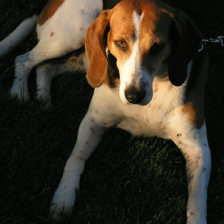
\includegraphics[width =
        .35\linewidth]{../repos/cockpit-paper/tex/fig/06_preprocessing/fig_samples/imagenetraw_vgg16_sample_00.png}}
      \Cshadowbox{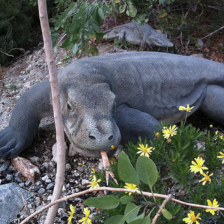
\includegraphics[width =
        .35\linewidth]{../repos/cockpit-paper/tex/fig/06_preprocessing/fig_samples/imagenetraw_vgg16_sample_01.png}}

      \Cshadowbox{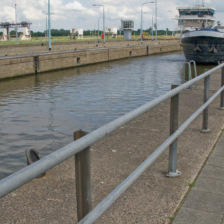
\includegraphics[width =
        .35\linewidth]{../repos/cockpit-paper/tex/fig/06_preprocessing/fig_samples/imagenetraw_vgg16_sample_02.png}}
      \Cshadowbox{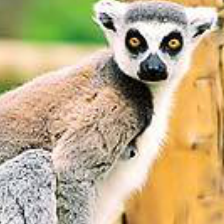
\includegraphics[width =
        .35\linewidth]{../repos/cockpit-paper/tex/fig/06_preprocessing/fig_samples/imagenetraw_vgg16_sample_03.png}}
    \end{minipage}
    \begin{minipage}{.49\linewidth}
      \input{figures/cockpit/06_preprocessing/default_style}
      \centering
      % customize "zmystyle" as you wish
      \pgfkeys{/pgfplots/zmystyle/.style={preprocessingexperimentdefault,
          ylabel={Gradient Element}
        }}
      \vspace{1.4\baselineskip}
      \tikzexternalenable
      \input{../repos/cockpit-paper/tex/fig/06_preprocessing/fig_histograms/imagenetraw_vgg16.tex}
      \tikzexternaldisable
    \end{minipage}
    \vspace{-2ex}
    \caption{Normalized Data}
    \label{cockpit::fig:data-pre-processing_norm_imagenet}
  \end{subfigure}
  \hfill
  \begin{subfigure}[t]{0.46\linewidth}
    \begin{minipage}{.49\linewidth}
      \Cshadowbox{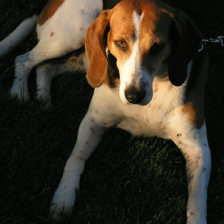
\includegraphics[width =
        .35\linewidth]{../repos/cockpit-paper/tex/fig/06_preprocessing/fig_samples/imagenetscale255_vgg16_sample_00.png}}
      \Cshadowbox{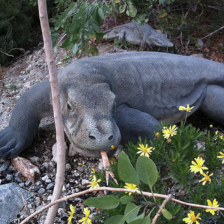
\includegraphics[width =
        .35\linewidth]{../repos/cockpit-paper/tex/fig/06_preprocessing/fig_samples/imagenetscale255_vgg16_sample_01.png}}

      \Cshadowbox{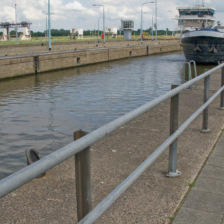
\includegraphics[width =
        .35\linewidth]{../repos/cockpit-paper/tex/fig/06_preprocessing/fig_samples/imagenetscale255_vgg16_sample_02.png}}
      \Cshadowbox{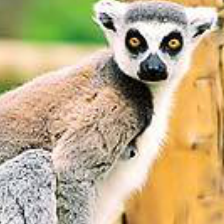
\includegraphics[width =
        .35\linewidth]{../repos/cockpit-paper/tex/fig/06_preprocessing/fig_samples/imagenetscale255_vgg16_sample_03.png}}
    \end{minipage}
    \begin{minipage}{.49\linewidth}
      \centering
      \input{figures/cockpit/06_preprocessing/default_style}
      % customize "zmystyle" as you wish
      \pgfkeys{/pgfplots/zmystyle/.style={preprocessingexperimentdefault,
          ylabel={Gradient Element}
        }}
      \vspace{1.4\baselineskip}
      \tikzexternalenable
      \input{../repos/cockpit-paper/tex/fig/06_preprocessing/fig_histograms/imagenetscale255_vgg16.tex}
      \tikzexternaldisable
    \end{minipage}
    \vspace{-2ex}
    \caption{Raw Data}
    \label{cockpit::fig:data-pre-processing_raw_imagenet}
  \end{subfigure}
  \caption{\textbf{Same inputs, different gradients on ImageNet.} This is
    structurally the same plot as \Cref{cockpit::fig:data-pre-processing}, but
    using \imagenet and \vgg.
    \subfigref{cockpit::fig:data-pre-processing_norm_imagenet} \emph{normalized}
    ($[0, 1]$) and \subfigref{cockpit::fig:data-pre-processing_raw_imagenet}
    \emph{raw} $([0, 255])$ images look identical in auto-scaled front-ends like
    \matplotlib's \robustInlinecode{imshow}. The gradient distribution on the \vgg model,
    however, is affected by this scaling.}
  \label{cockpit::fig:data-pre-processing_imagenet}
\end{figure*}

%%% Local Variables:
%%% mode: latex
%%% TeX-master: "../../../thesis"
%%% End:


%%% Local Variables:
%%% mode: latex
%%% TeX-master: "../thesis"
%%% End:

\subsection{Detecting Implicit Regularization of The
  Optimizer}\label{cockpit::app:implicit_regularization_exp}

In non-convex optimization, optimizers can converge to local minima with
different properties. Here, we illustrate this by investigating the effect of
sub-sampling noise on a simple task from
\cite{mulayoff2020unique,ginsburg2020regularization}.

We generate synthetic data $\sD = \{(x_n, y_n) \in \sR \times \sR
\}_{n=1}^{N=100}$ for a regression task with $x \sim \gN(\giventhat{x}{0, 1})$
with noisy observations $y = 1.4 x + \epsilon$ where $\epsilon \sim
\gN(\giventhat{\epsilon}{0,1})$. The model is a scalar net with parameters
$\vtheta = \begin{pmatrix} w_1 & w_2 \end{pmatrix}^\top \in \sR^2$, initialized
at $\vtheta_0 = \begin{pmatrix} 0.1 & 1.7 \end{pmatrix}^\top$, that produces
predictions $f_{\vtheta}(x) = w_2 w_1 x$. We seek to minimize the mean squared
error
\begin{equation*}
  \gL_\sD(\vtheta) = \frac{1}{N} \sum_{n=1}^{N} \left( f_{\vtheta}(x_n) - y_n \right)^2
\end{equation*}
and compare \sgd ($|\sB|=95$) with \gd ($|\sB|= N =100$) at a learning rate of
$0.1$ (see \Cref{cockpit::fig:implicit-regularization}).

We observe that the loss of both \sgd and \gd is almost identical. Using a noisy
gradient regularizes the Hessian's maximum eigenvalue though. It decreases in
later stages where the loss curve suggests that training has converged. This
regularization effect constitutes an important phenomenon that cannot be
observed by monitoring only the loss.

\pgfkeys{/pgfplots/regularizationdefault/.style={
    width=1.05\linewidth,
    height=0.8\linewidth,
    every axis plot/.append style={line width = 1.5pt},
    every axis background/.style={fill=white},
    ymajorticks=true,
    xmajorticks=true,
    tick pos = left,
    ylabel near ticks,
    xlabel near ticks,
    xtick align = inside,
    ytick align = inside,
    legend cell align = left,
    legend columns = 1,
    legend pos = north east,
    legend style = {
      fill opacity = 0.7,
      text opacity = 1,
      font = \footnotesize,
    },
    colorbar style = {font = \footnotesize},
    title style = {font = \footnotesize, inner ysep = 0ex},
    xticklabel style = {font = \footnotesize, inner xsep = 0ex},
    xlabel style = {font = \footnotesize},
    axis line style = {black},
    yticklabel style = {font = \footnotesize, inner ysep = -4ex},
    ylabel style = {font = \footnotesize},
    grid = major,
    grid style = {dashed}
  }
}

\begin{figure}[!th]
  \centering
	\begin{subfigure}[t]{0.495\textwidth}
    \centering
		\pgfkeys{/pgfplots/zmystyle/.style={regularizationdefault, ymin=0.6, ymax=1.1}}
    \tikzexternalenable
		% This file was created by tikzplotlib v0.9.7.
\begin{tikzpicture}

\definecolor{color0}{rgb}{0.12156862745098,0.466666666666667,0.705882352941177}
\definecolor{color1}{rgb}{1,0.498039215686275,0.0549019607843137}

\begin{axis}[
axis line style={white},
legend style={fill opacity=0.8, draw opacity=1, text opacity=1, draw=white!80!black},
log basis x={10},
tick align=outside,
xlabel={Iteration},
xmajorticks=false,
xmin=0.563970595937194, xmax=167345.603972783,
xmode=log,
xtick style={color=white!15!black},
ylabel={Mini-Batch Loss},
ymajorticks=false,
ymin=0.614918631315231, ymax=1.72726913094521,
zmystyle
]
\addplot [, color0]
table {%
0 1.65519058704376
1 1.01682019233704
2 0.780193150043488
3 0.775982201099396
4 0.737731337547302
5 0.771629452705383
6 0.738641858100891
7 0.745266854763031
8 0.772922933101654
9 0.748066663742065
10 0.77786260843277
11 0.769368886947632
12 0.775993466377258
13 0.769854426383972
14 0.780099034309387
15 0.732372939586639
16 0.76972508430481
17 0.77314555644989
18 0.787652790546417
19 0.731954038143158
20 0.753742933273315
21 0.760406374931335
22 0.772047460079193
24 0.752689599990845
25 0.768256425857544
27 0.772502541542053
28 0.745130240917206
30 0.73753297328949
32 0.775065541267395
34 0.7575803399086
36 0.748904526233673
38 0.78914475440979
40 0.774977564811707
42 0.770744025707245
45 0.771463930606842
48 0.724553644657135
51 0.750621318817139
54 0.786653280258179
57 0.740645587444305
60 0.780794203281403
64 0.765990436077118
68 0.772936582565308
72 0.764917433261871
76 0.75068473815918
81 0.763052582740784
86 0.766409575939178
91 0.779118478298187
96 0.779287576675415
102 0.694868266582489
108 0.753131628036499
114 0.745236694812775
121 0.769624173641205
128 0.733922481536865
136 0.763625741004944
144 0.771767735481262
153 0.778103351593018
162 0.76782751083374
172 0.770959913730621
182 0.778098523616791
193 0.747863173484802
204 0.767393231391907
217 0.747031450271606
230 0.761284053325653
243 0.788995981216431
258 0.78480863571167
273 0.725325763225555
289 0.788911044597626
307 0.757820010185242
325 0.701482534408569
344 0.786840677261353
365 0.75093948841095
387 0.793320834636688
410 0.733399331569672
434 0.790173828601837
460 0.789791882038116
488 0.772913932800293
517 0.747723639011383
547 0.767966389656067
580 0.769767463207245
615 0.777678191661835
651 0.732484042644501
690 0.765304982662201
731 0.779313802719116
775 0.752284646034241
821 0.751649916172028
870 0.763818562030792
922 0.763033270835876
977 0.76042252779007
1035 0.794110774993896
1096 0.770817458629608
1162 0.719465613365173
1231 0.773622274398804
1304 0.777041494846344
1382 0.752636194229126
1464 0.746034681797028
1552 0.756577551364899
1644 0.710349500179291
1742 0.788471639156342
1846 0.749858379364014
1956 0.751055300235748
2072 0.77653980255127
2196 0.743179202079773
2327 0.777839779853821
2465 0.765402734279633
2612 0.784416019916534
2768 0.675363481044769
2933 0.767980337142944
3107 0.77206939458847
3292 0.761081337928772
3489 0.780567407608032
3696 0.759546518325806
3917 0.772010743618011
4150 0.731160163879395
4397 0.778384268283844
4659 0.792823255062103
4937 0.780224800109863
5231 0.716187834739685
5542 0.732295513153076
5872 0.757798075675964
6222 0.783280313014984
6593 0.774591028690338
6985 0.76332038640976
7401 0.73084568977356
7842 0.744604051113129
8309 0.77698802947998
8804 0.770139813423157
9329 0.7605100274086
9884 0.745865881443024
10473 0.772988736629486
11097 0.784264206886292
11758 0.73901504278183
12458 0.665480017662048
13200 0.74626225233078
13987 0.765305399894714
14820 0.788454294204712
15702 0.783531785011292
16638 0.790920555591583
17629 0.723659753799438
18679 0.79127299785614
19791 0.776141047477722
20970 0.772833287715912
22219 0.73369562625885
23542 0.771220922470093
24945 0.785363912582397
26430 0.72164660692215
28005 0.788875877857208
29673 0.772274553775787
31440 0.764169812202454
33312 0.723604738712311
35297 0.758412897586823
37399 0.769568562507629
39626 0.782877564430237
41987 0.774317562580109
44487 0.74730920791626
47137 0.759216368198395
49945 0.75877833366394
52919 0.77678370475769
56071 0.770803034305573
59411 0.757794678211212
62949 0.775205314159393
66699 0.787786245346069
70671 0.761527419090271
74881 0.740764439105988
79340 0.766364872455597
84066 0.771571159362793
89073 0.774646580219269
94378 0.766631364822388
};
\addlegendentry{SGD}
\addplot [, color1]
table {%
0 1.67670774459839
1 1.00288474559784
2 0.814482688903809
3 0.769742786884308
4 0.761073589324951
5 0.759601593017578
6 0.759367525577545
7 0.759331345558167
8 0.759325861930847
9 0.759325087070465
10 0.759324848651886
11 0.759324848651886
12 0.759324908256531
13 0.759324848651886
14 0.759324848651886
15 0.759324848651886
16 0.759324848651886
17 0.759324848651886
18 0.759324908256531
19 0.759324848651886
20 0.759324848651886
21 0.759324848651886
22 0.759324848651886
24 0.759324789047241
25 0.759324848651886
27 0.759324848651886
28 0.759324848651886
30 0.759324848651886
32 0.759324848651886
34 0.759324848651886
36 0.759324908256531
38 0.759324848651886
40 0.759324848651886
42 0.759324848651886
45 0.759324908256531
48 0.759324848651886
51 0.759324848651886
54 0.759324848651886
57 0.759324848651886
60 0.759324848651886
64 0.759324848651886
68 0.759324848651886
72 0.759324848651886
76 0.759324848651886
81 0.759324908256531
86 0.759324789047241
91 0.759324848651886
96 0.759324908256531
102 0.759324848651886
108 0.759324848651886
114 0.759324908256531
121 0.759324848651886
128 0.759324848651886
136 0.759324789047241
144 0.759324908256531
153 0.759324848651886
162 0.759324848651886
172 0.759324908256531
182 0.759324908256531
193 0.759324848651886
204 0.759324908256531
217 0.759324908256531
230 0.759324908256531
243 0.759324848651886
258 0.759324848651886
273 0.759324908256531
289 0.759324848651886
307 0.759324848651886
325 0.759324848651886
344 0.759324789047241
365 0.759324848651886
387 0.759324848651886
410 0.759324908256531
434 0.759324848651886
460 0.759324848651886
488 0.759324848651886
517 0.759324848651886
547 0.759324848651886
580 0.759324908256531
615 0.759324908256531
651 0.759324848651886
690 0.759324848651886
731 0.759324848651886
775 0.759324789047241
821 0.759324848651886
870 0.759324848651886
922 0.759324848651886
977 0.759324848651886
1035 0.759324908256531
1096 0.759324908256531
1162 0.759324789047241
1231 0.759324848651886
1304 0.759324848651886
1382 0.759324848651886
1464 0.759324848651886
1552 0.759324848651886
1644 0.759324848651886
1742 0.759324908256531
1846 0.759324848651886
1956 0.759324908256531
2072 0.759324908256531
2196 0.759324908256531
2327 0.759324789047241
2465 0.759324908256531
2612 0.759324848651886
2768 0.759324848651886
2933 0.759324848651886
3107 0.759324848651886
3292 0.759324908256531
3489 0.759324908256531
3696 0.759324908256531
3917 0.759324848651886
4150 0.759324848651886
4397 0.759324848651886
4659 0.759324848651886
4937 0.759324848651886
5231 0.759324848651886
5542 0.759324848651886
5872 0.759324908256531
6222 0.759324908256531
6593 0.759324848651886
6985 0.759324908256531
7401 0.759324908256531
7842 0.759324848651886
8309 0.759324848651886
8804 0.759324908256531
9329 0.759324848651886
9884 0.759324908256531
10473 0.759324848651886
11097 0.759324908256531
11758 0.759324848651886
12458 0.759324848651886
13200 0.759324848651886
13987 0.759324908256531
14820 0.759324908256531
15702 0.759324848651886
16638 0.759324848651886
17629 0.759324848651886
18679 0.759324908256531
19791 0.759324908256531
20970 0.759324848651886
22219 0.759324848651886
23542 0.759324848651886
24945 0.759324848651886
26430 0.759324908256531
28005 0.759324848651886
29673 0.759324848651886
31440 0.759324789047241
33312 0.759324848651886
35297 0.759324848651886
37399 0.759324789047241
39626 0.759324908256531
41987 0.759324848651886
44487 0.759324848651886
47137 0.759324848651886
49945 0.759324848651886
52919 0.759324848651886
56071 0.759324848651886
59411 0.759324908256531
62949 0.759324789047241
66699 0.759324848651886
70671 0.759324848651886
74881 0.759324848651886
79340 0.759324848651886
84066 0.759324848651886
89073 0.759324848651886
94378 0.759324908256531
};
\addlegendentry{GD}
\end{axis}

\end{tikzpicture}

    \tikzexternaldisable
	\end{subfigure}
	\hfill
	\begin{subfigure}[t]{0.495\textwidth}
    \centering
		\pgfkeys{/pgfplots/zmystyle/.style={regularizationdefault,
        legend style = {
          opacity = 0,
          fill opacity = 0,
          text opacity = 0,
        },
        ylabel = {Max.\,Hessian eigenvalue}
      }}
    \tikzexternalenable
		% This file was created by tikzplotlib v0.9.7.
\begin{tikzpicture}

\definecolor{color0}{rgb}{0.12156862745098,0.466666666666667,0.705882352941177}
\definecolor{color1}{rgb}{1,0.498039215686275,0.0549019607843137}

\begin{axis}[
axis line style={white},
legend style={fill opacity=0.8, draw opacity=1, text opacity=1, draw=white!80!black},
log basis x={10},
tick align=outside,
xlabel={Iteration},
xmajorticks=false,
xmin=0.563970595937194, xmax=167345.603972783,
xmode=log,
xtick style={color=white!15!black},
ylabel={Maximum Hessian eigenvalue},
ymajorticks=false,
ymin=3.85510742664337, ymax=6.68519914150238,
zmystyle
]
\addplot [, color0]
table {%
0 5.01858520507812
1 4.91631031036377
2 5.16143560409546
3 5.60115337371826
4 5.79127502441406
5 6.0561056137085
6 6.26061916351318
7 6.19245529174805
8 6.1329493522644
9 6.05357074737549
10 5.97355842590332
11 6.05519437789917
12 6.31369209289551
13 6.22404289245605
14 6.33904695510864
15 5.68460321426392
16 6.16733026504517
17 6.17319679260254
18 6.14776849746704
19 6.2695107460022
20 6.03493785858154
21 6.15226316452026
22 6.19907712936401
24 5.59337615966797
25 6.36163806915283
27 6.35177993774414
28 6.22747230529785
30 5.91255331039429
32 6.19828081130981
34 6.39521312713623
36 6.0371265411377
38 6.43193244934082
40 6.14503479003906
42 6.25523281097412
45 6.05292510986328
48 5.67981719970703
51 6.36472225189209
54 6.06869220733643
57 6.18863964080811
60 5.93778562545776
64 6.12580823898315
68 6.18363857269287
72 6.01109552383423
76 6.02523136138916
81 6.21799850463867
86 6.18191480636597
91 6.55655860900879
96 6.31975746154785
102 6.05267763137817
108 6.0778636932373
114 6.01467657089233
121 6.24698925018311
128 6.04640293121338
136 6.24112749099731
144 6.31688690185547
153 6.28657817840576
162 6.13792037963867
172 5.65208387374878
182 6.30600261688232
193 5.98742771148682
204 5.71659326553345
217 5.84029388427734
230 6.0068564414978
243 6.3081259727478
258 6.39043521881104
273 6.14346885681152
289 6.18961191177368
307 6.13053369522095
325 6.17688846588135
344 5.90940189361572
365 5.89127063751221
387 5.98564434051514
410 6.25674438476562
434 5.93166160583496
460 6.01510143280029
488 6.29282379150391
517 6.3133373260498
547 5.89875364303589
580 5.78323602676392
615 6.22842979431152
651 6.12653160095215
690 6.13379669189453
731 6.08839702606201
775 6.19680023193359
821 6.05588006973267
870 6.21298170089722
922 6.0586724281311
977 5.70560264587402
1035 6.05281639099121
1096 6.12884950637817
1162 5.72979116439819
1231 5.75020885467529
1304 5.78489637374878
1382 6.24677515029907
1464 5.72618103027344
1552 6.16928005218506
1644 5.99916076660156
1742 6.31236791610718
1846 5.42526912689209
1956 6.01460218429565
2072 6.17887306213379
2196 5.93650770187378
2327 6.21088695526123
2465 5.92963600158691
2612 5.98927402496338
2768 6.04936790466309
2933 5.9457950592041
3107 6.15447568893433
3292 6.04442024230957
3489 5.88113212585449
3696 6.0181360244751
3917 5.82596063613892
4150 5.97462749481201
4397 5.84421348571777
4659 5.84129619598389
4937 5.80539751052856
5231 6.00247669219971
5542 5.8760838508606
5872 5.92244338989258
6222 5.69848346710205
6593 5.64358997344971
6985 5.6120719909668
7401 5.73087453842163
7842 5.67744302749634
8309 5.43394136428833
8804 5.7706823348999
9329 5.68305492401123
9884 5.22680282592773
10473 5.09199523925781
11097 5.7391529083252
11758 5.49506330490112
12458 5.29003858566284
13200 5.21850109100342
13987 5.15451717376709
14820 5.25626420974731
15702 5.2664647102356
16638 5.09290647506714
17629 5.06191682815552
18679 5.22023582458496
19791 4.99110126495361
20970 5.13607454299927
22219 4.82361221313477
23542 4.96726989746094
24945 4.517502784729
26430 4.89909362792969
28005 4.69721984863281
29673 4.44070720672607
31440 4.71606779098511
33312 4.43321752548218
35297 4.52913951873779
37399 4.35525035858154
39626 4.48494052886963
41987 4.43455600738525
44487 4.4298300743103
47137 4.41794347763062
49945 4.16174602508545
52919 4.41815376281738
56071 4.30182790756226
59411 4.18179321289062
62949 4.38689374923706
66699 4.22925329208374
70671 4.26896953582764
74881 4.2410717010498
79340 4.02750778198242
84066 3.98374795913696
89073 4.10416793823242
94378 4.25959587097168
};
\addlegendentry{SGD}
\addplot [, color1]
table {%
0 5.19412231445312
1 4.89158582687378
2 5.36561346054077
3 5.75625705718994
4 5.95861196517944
5 6.04718065261841
6 6.08332633972168
7 6.09766292572021
8 6.10328483581543
9 6.10547971725464
10 6.10633707046509
11 6.10666942596436
12 6.10679912567139
13 6.106849193573
14 6.10686922073364
15 6.10687732696533
16 6.10687875747681
17 6.1068811416626
18 6.1068811416626
19 6.10688161849976
20 6.10688161849976
21 6.10688161849976
22 6.10688161849976
24 6.10688161849976
25 6.1068811416626
27 6.10688209533691
28 6.1068811416626
30 6.10688161849976
32 6.10688161849976
34 6.10688161849976
36 6.10688161849976
38 6.10688161849976
40 6.1068811416626
42 6.10688161849976
45 6.10688161849976
48 6.10688257217407
51 6.10688209533691
54 6.10688161849976
57 6.10688209533691
60 6.10688161849976
64 6.10688209533691
68 6.1068811416626
72 6.10688161849976
76 6.10688161849976
81 6.10688257217407
86 6.10688161849976
91 6.1068811416626
96 6.10688209533691
102 6.10688257217407
108 6.10688161849976
114 6.10688209533691
121 6.1068811416626
128 6.10688257217407
136 6.10688161849976
144 6.10688209533691
153 6.10688161849976
162 6.10688209533691
172 6.10688161849976
182 6.10688161849976
193 6.1068811416626
204 6.10688161849976
217 6.10688257217407
230 6.1068811416626
243 6.10688209533691
258 6.1068811416626
273 6.1068811416626
289 6.10688161849976
307 6.10688161849976
325 6.1068811416626
344 6.10688161849976
365 6.10688161849976
387 6.10688161849976
410 6.10688209533691
434 6.10688161849976
460 6.10688161849976
488 6.1068811416626
517 6.10688161849976
547 6.10688161849976
580 6.10688209533691
615 6.10688161849976
651 6.1068811416626
690 6.1068811416626
731 6.1068811416626
775 6.1068811416626
821 6.1068811416626
870 6.10688209533691
922 6.10688161849976
977 6.10688161849976
1035 6.10688161849976
1096 6.10688161849976
1162 6.10688161849976
1231 6.1068811416626
1304 6.10688209533691
1382 6.10688161849976
1464 6.10688161849976
1552 6.1068811416626
1644 6.1068811416626
1742 6.10688161849976
1846 6.10688209533691
1956 6.10688161849976
2072 6.1068811416626
2196 6.10688161849976
2327 6.1068811416626
2465 6.10688161849976
2612 6.10688161849976
2768 6.10688161849976
2933 6.10688209533691
3107 6.10688257217407
3292 6.10688161849976
3489 6.10688257217407
3696 6.10688161849976
3917 6.1068811416626
4150 6.10688209533691
4397 6.1068811416626
4659 6.10688161849976
4937 6.10688209533691
5231 6.10688161849976
5542 6.1068811416626
5872 6.10688161849976
6222 6.10688209533691
6593 6.1068811416626
6985 6.10688161849976
7401 6.10688209533691
7842 6.10688161849976
8309 6.10688209533691
8804 6.10688161849976
9329 6.10688161849976
9884 6.1068811416626
10473 6.1068811416626
11097 6.10688161849976
11758 6.10688161849976
12458 6.10688161849976
13200 6.1068811416626
13987 6.1068811416626
14820 6.1068811416626
15702 6.10688161849976
16638 6.10688161849976
17629 6.10688161849976
18679 6.10688161849976
19791 6.1068811416626
20970 6.1068811416626
22219 6.1068811416626
23542 6.10688209533691
24945 6.10688161849976
26430 6.10688209533691
28005 6.10688209533691
29673 6.1068811416626
31440 6.10688161849976
33312 6.10688209533691
35297 6.10688161849976
37399 6.10688161849976
39626 6.10688209533691
41987 6.10688161849976
44487 6.10688161849976
47137 6.10688161849976
49945 6.1068811416626
52919 6.10688209533691
56071 6.10688209533691
59411 6.10688161849976
62949 6.10688161849976
66699 6.10688161849976
70671 6.10688161849976
74881 6.10688161849976
79340 6.10688161849976
84066 6.10688161849976
89073 6.1068811416626
94378 6.10688161849976
};
\addlegendentry{GD}
\end{axis}

\end{tikzpicture}

    \tikzexternaldisable
	\end{subfigure}
  \vspace{1ex}
  \begin{subfigure}{1.0\linewidth}
    \centering
		\pgfkeys{/pgfplots/zmystyle/.style={regularizationdefault,
        width = 0.91\linewidth,
        height = 0.6695*0.91*\linewidth,
        legend style = {
          opacity = 0,
          fill opacity = 0,
          text opacity = 0,
        },
        xmajorticks=true,
        ymajorticks=true,
      }}
    \tikzexternalenable
    % This file was created by tikzplotlib v0.9.7.
\begin{tikzpicture}

\definecolor{color0}{rgb}{0.12156862745098,0.466666666666667,0.705882352941177}
\definecolor{color1}{rgb}{1,0.498039215686275,0.0549019607843137}

\begin{axis}[
axis line style={white},
colorbar,
colormap={mymap}{[1pt]
  rgb(0pt)=(1,1,0.850980392156863);
  rgb(1pt)=(0.929411764705882,0.972549019607843,0.694117647058824);
  rgb(2pt)=(0.780392156862745,0.913725490196078,0.705882352941177);
  rgb(3pt)=(0.498039215686275,0.803921568627451,0.733333333333333);
  rgb(4pt)=(0.254901960784314,0.713725490196078,0.768627450980392);
  rgb(5pt)=(0.113725490196078,0.568627450980392,0.752941176470588);
  rgb(6pt)=(0.133333333333333,0.368627450980392,0.658823529411765);
  rgb(7pt)=(0.145098039215686,0.203921568627451,0.580392156862745);
  rgb(8pt)=(0.0313725490196078,0.113725490196078,0.345098039215686)
},
legend style={fill opacity=0.8, draw opacity=1, text opacity=1, draw=white!80!black},
point meta max=33.3554496765137,
point meta min=0.759324848651886,
tick align=outside,
title={Loss landscape},
xlabel={\(\displaystyle \theta_1\)},
xmajorticks=false,
xmin=-1, xmax=2.5,
xtick style={color=white!15!black},
ylabel={\(\displaystyle \theta_2\)},
ymajorticks=false,
ymin=-0.5, ymax=3,
zmystyle
]
\addplot graphics [,xmin=-1, xmax=2.5, ymin=-0.5, ymax=3] {Trajectory-000.png};
\addplot [, color0]
table {%
0.100000001490116 1.70000004768372
0.390511572360992 1.7170889377594
0.546473205089569 1.75255870819092
0.601417779922485 1.76969122886658
0.639493048191071 1.78263092041016
0.645879983901978 1.78492212295532
0.667922377586365 1.79289829730988
0.669110357761383 1.79334080219269
0.682194948196411 1.79822278022766
0.674466907978058 1.79529094696045
0.663153052330017 1.79104053974152
0.673606514930725 1.79491102695465
0.675003290176392 1.79543519020081
0.678699016571045 1.79682457447052
0.685095965862274 1.79924082756042
0.687204122543335 1.80004358291626
0.691844761371613 1.80181527137756
0.671525537967682 1.79401326179504
0.675070106983185 1.79534006118774
0.67482715845108 1.79524874687195
0.678539335727692 1.79664409160614
0.685560762882233 1.7992959022522
0.67389988899231 1.79485297203064
0.677536308765411 1.79621696472168
0.700529396533966 1.80489003658295
0.682436764240265 1.79790055751801
0.681613385677338 1.7975879907608
0.677117347717285 1.79583013057709
0.692475318908691 1.80160808563232
0.680085301399231 1.79686343669891
0.690684139728546 1.80087828636169
0.689901888370514 1.80054640769958
0.68423718214035 1.79837930202484
0.682424306869507 1.79768741130829
0.675705194473267 1.79513609409332
0.675473153591156 1.79498684406281
0.698002457618713 1.80348515510559
0.677664995193481 1.79566705226898
0.671689748764038 1.79340803623199
0.670520484447479 1.79295492172241
0.678237795829773 1.79584860801697
0.672419190406799 1.79344725608826
0.685892820358276 1.79848670959473
0.680178642272949 1.7962874174118
0.685978591442108 1.79844427108765
0.694296002388 1.80159783363342
0.711118221282959 1.80797255039215
0.675868630409241 1.79425501823425
0.684127986431122 1.79733657836914
0.679848849773407 1.79566979408264
0.669373571872711 1.79165542125702
0.679888606071472 1.79551303386688
0.662135541439056 1.78879928588867
0.686899542808533 1.79779970645905
0.682054400444031 1.79579043388367
0.672400176525116 1.7919909954071
0.680885851383209 1.79514026641846
0.667153120040894 1.78990614414215
0.679344117641449 1.79442346096039
0.673126935958862 1.79201233386993
0.670550942420959 1.79096555709839
0.69197142124176 1.79880881309509
0.672725915908813 1.79119396209717
0.676092565059662 1.79214191436768
0.688663899898529 1.79669153690338
0.681666493415833 1.79389941692352
0.677907943725586 1.79229915142059
0.673436224460602 1.79007911682129
0.68997323513031 1.79620814323425
0.667576611042023 1.78752589225769
0.682157278060913 1.79277646541595
0.679268181324005 1.79123222827911
0.681079208850861 1.79162502288818
0.677574813365936 1.78988242149353
0.67927086353302 1.79004609584808
0.697462141513824 1.79662251472473
0.69139176607132 1.79365348815918
0.687649428844452 1.79169237613678
0.682355523109436 1.78918492794037
0.675151944160461 1.78578960895538
0.67628139257431 1.78551888465881
0.675973236560822 1.78479135036469
0.665274679660797 1.77992808818817
0.678472220897675 1.78403651714325
0.689973175525665 1.78784000873566
0.681166648864746 1.78333806991577
0.691523969173431 1.78662049770355
0.698261976242065 1.78783130645752
0.690599858760834 1.78375256061554
0.680019974708557 1.77813601493835
0.688908398151398 1.78057253360748
0.698104679584503 1.78271543979645
0.67931067943573 1.77420496940613
0.684651434421539 1.77530860900879
0.693451106548309 1.77726054191589
0.689227163791656 1.77445876598358
0.680094182491302 1.76916575431824
0.696024477481842 1.77381980419159
0.676648080348969 1.76468467712402
0.681325316429138 1.7649313211441
0.68862909078598 1.76631033420563
0.693156957626343 1.76604175567627
0.700364649295807 1.76705718040466
0.7011958360672 1.76529848575592
0.687162697315216 1.75772929191589
0.703916668891907 1.76169896125793
0.689925253391266 1.75330626964569
0.70111882686615 1.75461566448212
0.695941746234894 1.74926269054413
0.699183106422424 1.74723780155182
0.696930766105652 1.74242079257965
0.710143327713013 1.74268937110901
0.698858141899109 1.73455560207367
0.709864377975464 1.73439800739288
0.704060018062592 1.72810399532318
0.698992013931274 1.72063815593719
0.712297260761261 1.72095036506653
0.717435717582703 1.7179012298584
0.712529122829437 1.71006381511688
0.719913721084595 1.70747792720795
0.719109177589417 1.70160639286041
0.719201445579529 1.69564807415009
0.726583480834961 1.69265925884247
0.724139869213104 1.68445897102356
0.719537675380707 1.67515122890472
0.74134373664856 1.67590343952179
0.740000069141388 1.66538965702057
0.730468451976776 1.65302991867065
0.740104854106903 1.64824032783508
0.76548433303833 1.65183210372925
0.744733691215515 1.63146710395813
0.746873617172241 1.62325477600098
0.753918051719666 1.61548483371735
0.765423655509949 1.61043667793274
0.773338854312897 1.60266101360321
0.773339629173279 1.59142887592316
0.76962685585022 1.57759571075439
0.778478145599365 1.56945598125458
0.793064177036285 1.56236958503723
0.792321801185608 1.54660928249359
0.79296088218689 1.53167915344238
0.792017102241516 1.51534283161163
0.815773010253906 1.51425313949585
0.818939983844757 1.50040066242218
0.82924497127533 1.48936939239502
0.819665551185608 1.46620404720306
0.837881088256836 1.45742213726044
0.848906576633453 1.44540286064148
0.84745717048645 1.42533433437347
0.871433675289154 1.42067611217499
0.862388014793396 1.39525926113129
0.880145847797394 1.38803493976593
0.897489786148071 1.3785206079483
0.903302729129791 1.36190438270569
0.913372099399567 1.34719264507294
0.916217088699341 1.32893395423889
0.953232765197754 1.33372986316681
0.942984879016876 1.3056834936142
0.944588005542755 1.28611779212952
0.962793827056885 1.27936899662018
0.963907539844513 1.2592408657074
0.999159157276154 1.26485371589661
1.00393545627594 1.24771106243134
0.999233841896057 1.22480249404907
1.00601613521576 1.21015644073486
1.01214456558228 1.1964567899704
1.02476096153259 1.18976318836212
};
\addlegendentry{SGD}
\addplot [, color1]
table {%
0.100000001490116 1.70000004768372
0.396201580762863 1.71742367744446
0.5503870844841 1.7529935836792
0.625281095504761 1.77650809288025
0.658266365528107 1.78811800479889
0.671868860721588 1.79312551021576
0.677294850349426 1.79515862464905
0.679428040981293 1.79596340656281
0.680261731147766 1.79627883434296
0.680586755275726 1.79640197753906
0.680713355541229 1.79644989967346
0.680762708187103 1.79646861553192
0.680781900882721 1.79647588729858
0.680789351463318 1.79647874832153
0.680792272090912 1.79647982120514
0.680793404579163 1.7964802980423
0.680793821811676 1.79648041725159
0.68079400062561 1.79648053646088
0.680794060230255 1.79648053646088
0.6807941198349 1.79648053646088
0.6807941198349 1.79648053646088
0.6807941198349 1.79648053646088
0.6807941198349 1.79648053646088
0.6807941198349 1.79648053646088
0.6807941198349 1.79648053646088
0.6807941198349 1.79648053646088
0.6807941198349 1.79648053646088
0.6807941198349 1.79648053646088
0.6807941198349 1.79648053646088
0.6807941198349 1.79648053646088
0.6807941198349 1.79648053646088
0.6807941198349 1.79648053646088
0.6807941198349 1.79648053646088
0.6807941198349 1.79648053646088
0.6807941198349 1.79648053646088
0.6807941198349 1.79648053646088
0.6807941198349 1.79648053646088
0.6807941198349 1.79648053646088
0.6807941198349 1.79648053646088
0.6807941198349 1.79648053646088
0.6807941198349 1.79648053646088
0.6807941198349 1.79648053646088
0.6807941198349 1.79648053646088
0.6807941198349 1.79648053646088
0.6807941198349 1.79648053646088
0.6807941198349 1.79648053646088
0.6807941198349 1.79648053646088
0.6807941198349 1.79648053646088
0.6807941198349 1.79648053646088
0.6807941198349 1.79648053646088
0.6807941198349 1.79648053646088
0.6807941198349 1.79648053646088
0.6807941198349 1.79648053646088
0.6807941198349 1.79648053646088
0.6807941198349 1.79648053646088
0.6807941198349 1.79648053646088
0.6807941198349 1.79648053646088
0.6807941198349 1.79648053646088
0.6807941198349 1.79648053646088
0.6807941198349 1.79648053646088
0.6807941198349 1.79648053646088
0.6807941198349 1.79648053646088
0.6807941198349 1.79648053646088
0.6807941198349 1.79648053646088
0.6807941198349 1.79648053646088
0.6807941198349 1.79648053646088
0.6807941198349 1.79648053646088
0.6807941198349 1.79648053646088
0.6807941198349 1.79648053646088
0.6807941198349 1.79648053646088
0.6807941198349 1.79648053646088
0.6807941198349 1.79648053646088
0.6807941198349 1.79648053646088
0.6807941198349 1.79648053646088
0.6807941198349 1.79648053646088
0.6807941198349 1.79648053646088
0.6807941198349 1.79648053646088
0.6807941198349 1.79648053646088
0.6807941198349 1.79648053646088
0.6807941198349 1.79648053646088
0.6807941198349 1.79648053646088
0.6807941198349 1.79648053646088
0.6807941198349 1.79648053646088
0.6807941198349 1.79648053646088
0.6807941198349 1.79648053646088
0.6807941198349 1.79648053646088
0.6807941198349 1.79648053646088
0.6807941198349 1.79648053646088
0.6807941198349 1.79648053646088
0.6807941198349 1.79648053646088
0.6807941198349 1.79648053646088
0.6807941198349 1.79648053646088
0.6807941198349 1.79648053646088
0.6807941198349 1.79648053646088
0.6807941198349 1.79648053646088
0.6807941198349 1.79648053646088
0.6807941198349 1.79648053646088
0.6807941198349 1.79648053646088
0.6807941198349 1.79648053646088
0.6807941198349 1.79648053646088
0.6807941198349 1.79648053646088
0.6807941198349 1.79648053646088
0.6807941198349 1.79648053646088
0.6807941198349 1.79648053646088
0.6807941198349 1.79648053646088
0.6807941198349 1.79648053646088
0.6807941198349 1.79648053646088
0.6807941198349 1.79648053646088
0.6807941198349 1.79648053646088
0.6807941198349 1.79648053646088
0.6807941198349 1.79648053646088
0.6807941198349 1.79648053646088
0.6807941198349 1.79648053646088
0.6807941198349 1.79648053646088
0.6807941198349 1.79648053646088
0.6807941198349 1.79648053646088
0.6807941198349 1.79648053646088
0.6807941198349 1.79648053646088
0.6807941198349 1.79648053646088
0.6807941198349 1.79648053646088
0.6807941198349 1.79648053646088
0.6807941198349 1.79648053646088
0.6807941198349 1.79648053646088
0.6807941198349 1.79648053646088
0.6807941198349 1.79648053646088
0.6807941198349 1.79648053646088
0.6807941198349 1.79648053646088
0.6807941198349 1.79648053646088
0.6807941198349 1.79648053646088
0.6807941198349 1.79648053646088
0.6807941198349 1.79648053646088
0.6807941198349 1.79648053646088
0.6807941198349 1.79648053646088
0.6807941198349 1.79648053646088
0.6807941198349 1.79648053646088
0.6807941198349 1.79648053646088
0.6807941198349 1.79648053646088
0.6807941198349 1.79648053646088
0.6807941198349 1.79648053646088
0.6807941198349 1.79648053646088
0.6807941198349 1.79648053646088
0.6807941198349 1.79648053646088
0.6807941198349 1.79648053646088
0.6807941198349 1.79648053646088
0.6807941198349 1.79648053646088
0.6807941198349 1.79648053646088
0.6807941198349 1.79648053646088
0.6807941198349 1.79648053646088
0.6807941198349 1.79648053646088
0.6807941198349 1.79648053646088
0.6807941198349 1.79648053646088
0.6807941198349 1.79648053646088
0.6807941198349 1.79648053646088
0.6807941198349 1.79648053646088
0.6807941198349 1.79648053646088
0.6807941198349 1.79648053646088
0.6807941198349 1.79648053646088
0.6807941198349 1.79648053646088
0.6807941198349 1.79648053646088
0.6807941198349 1.79648053646088
0.6807941198349 1.79648053646088
0.6807941198349 1.79648053646088
0.6807941198349 1.79648053646088
0.6807941198349 1.79648053646088
0.6807941198349 1.79648053646088
0.6807941198349 1.79648053646088
0.6807941198349 1.79648053646088
};
\addlegendentry{GD}
\end{axis}

\end{tikzpicture}

    \tikzexternaldisable
  \end{subfigure}
  \caption{\textbf{Observing implicit regularization of the optimizer with
      \cockpittitle} through a comparison of \sgd and \gd on a synthetic problem
    inspired by \cite{mulayoff2020unique, ginsburg2020regularization} (details
    in the text). \textit{Top left:} The mini-batch loss of both optimizers
    looks similar. \textit{Top right:} Noise due to mini-batching regularizes
    the Hessian's maximum eigenvalue in stages where the loss suggests that
    training has converged. \textit{Bottom:} Optimization trajectories in
    parameter space. SGD is attracted to the flattest minimum.}
	  \label{cockpit::fig:implicit-regularization}
\end{figure}

%%% Local Variables:
%%% mode: latex
%%% TeX-master: "../thesis"
%%% End:


\section{Implementation Details \& Additional
  Benchmarks}\label{cockpit::app:benchmarks}
In this section, we provide more details about our implementation
(\Cref{cockpit::app:hooks_benchmarks}) to access the desired quantities with as
little overhead as possible. Additionally, we present more benchmarks for
individual instruments (\Cref{cockpit::app:benchmark-instruments}) and \cockpit
configurations (\Cref{cockpit::app:benchmark-configuration}). These are similar
but extended versions of the ones presented in
\Cref{cockpit::fig:benchmark-instruments,cockpit::fig:benchmark_heatmap} in the
main text. Lastly, we benchmark different implementations of computing the
two-dimensional gradient histogram (\Cref{cockpit::app:histograms}), identifying
a computational bottleneck for its current GPU implementation.

\subsubsection{Hardware Details}

We conducted benchmarks on the following setup:
\begin{itemize}
\item \textbf{CPU:} Intel Core i7-8700K CPU @ 3.70\,GHz × 12 (32\,GB)
\item \textbf{GPU:} NVIDIA GeForce RTX 2080 Ti (11\,GB)
\end{itemize}

\subsubsection{Test Problem Details}

The experiments in this paper rely mostly on optimization problems provided by
the \deepobs benchmark suite \citep{schneider2019deepobs}. If not stated
otherwise, we use the default training details suggested by \deepobs, that are
summarized below. For more details see the original paper.
\begin{itemize}
\item \textbf{Quadratic Deep:} A stochastic quadratic problem with an
  eigenspectrum similar to what has been reported for neural nets. Default batch
  size $128$, default number of epochs $100$.
\item \textbf{\mnist Log. Reg.:} Multinomial logistic regression on \mnist
  \citep{lecun1998gradient}. Default batch size $128$, default number of epochs $50$.
\item \textbf{\mnist \mlp:} Multi-layer perceptron on \mnist.
  Default batch size $128$, default number of epochs $100$.
\item \textbf{\fmnist \mlp:} Multi-layer perceptron on \fmnist
  \citep{xiao2017fashion}. Default batch size $128$, default number of epochs $100$.
\item \textbf{\fmnist \twoctwod:} A two convolutional and two dense layered
  neural network on \fmnist. Default batch size $128$, default number of epochs
  $100$.
\item \textbf{\cifarten \threecthreed:} A three convolutional and three dense
  layered neural network on \cifarten \citep{krizhevsky2009learning}. Default batch size
  $128$, default number of epochs $100$.
\item \textbf{\cifarhun \allcnnc:} All Convolutional Neural Network C (\allcnnc
  \citep{springenberg2015striving}) on \cifarhun \citep{krizhevsky2009learning}. Default batch
  size $256$, default number of epochs $350$.
\item \textbf{\svhn \threecthreed:} A three convolutional and three dense
  layered neural network on \svhn \citep{netzer2011reading}. Default batch size $128$,
  default number of epochs $100$.
\end{itemize}

\subsection{Hooks \& Memory Benchmarks}\label{cockpit::app:hooks_benchmarks}

To improve memory consumption, we compact information during the backward pass
by adding hooks to the neural network's layers. These are executed after
\backpack extensions and have access to the quantities computed therein. They
compress information to what is requested by a quantity and free the memory
occupied by \backpack buffers. Such savings primarily depend on the parameter
distribution over layers, and are bigger for more balanced architectures
(compare \Cref{cockpit::fig:memory-benchmark}).


\subsubsection{Example}

Say, we want to compute a histogram over the $|\sB| \times D$ individual
gradient elements of a network. Suppose that $|\sB| = 128$ and the model is
\deepobs's \cifarten \threecthreed test problem with $895,210$ parameters. Given
that every parameter is stored in single precision, the model requires $895,210
\times 4\,\text{Bytes} \approx 3.41\,\text{MB}$.
% computation performed with https://www.gbmb.org/bytes-to-mb, MB in binary
Storing the individual gradients will require $128 \times 895,210 \times
4\,\text{Bytes} \approx 437\,\text{MB}$ (for larger networks this quickly
exceeds the available memory as the individual gradients occupy $|\sB|$ times
the model size). If instead, the layer-wise individual gradients are condensed
into histograms of negligible size and immediately freed afterwards during
backpropagation, the maximum memory overhead reduces to storing the individual
gradients of the largest layer. For our example, the largest layer has
$589,824$ parameters, and the associated individual gradients will require $128
\times 589,824\times 4\,\text{Bytes} \approx 288\,\text{MB}$, saving roughly
$149\,\text{MB}$ of RAM. In practice, we observe these expected savings, see
\Cref{cockpit::fig:memory-benchmark-cifar10}.

\pgfkeys{/pgfplots/memorybenchmarkdefault/.style={
    enlarge x limits=-0.05,
    width=1.0\linewidth,
    height=0.45\linewidth,
    every axis plot/.append style={line width = 1.5pt},
    ymin=0,
    tick pos = left,
    ylabel near ticks,
    xlabel near ticks,
    xtick align = inside,
    ytick align = inside,
    legend cell align = left,
    legend columns = 1,
    legend pos = south east,
    legend style = {
      fill opacity = 0.7,
      text opacity = 1,
      font = \footnotesize,
    },
    xticklabel style = {font = \footnotesize, inner xsep = -5ex},
    xlabel style = {font = \footnotesize},
    axis line style = {black},
    yticklabel style = {font = \footnotesize, inner ysep = 0ex},
    ylabel style = {font = \footnotesize},
    title style = {font = \footnotesize, inner ysep = -3ex},
    grid = major,
    grid style = {dashed}
  }
}

\captionsetup[subfigure]{justification=justified,singlelinecheck=false}

\begin{figure}[!bt]
  \centering
  \begin{subfigure}[t]{0.99\textwidth}
    \pgfkeys{/pgfplots/zmystyle/.style={ memorybenchmarkdefault, xlabel = {},
        legend pos = north west}}
    \caption{\fmnist \twoctwod}
    \tikzexternalenable
    % This file was created by tikzplotlib v0.9.8.
\begin{tikzpicture}

\definecolor{color0}{rgb}{0.894117647058824,0.101960784313725,0.109803921568627}
\definecolor{color1}{rgb}{0.301960784313725,0.686274509803922,0.290196078431373}
\definecolor{color2}{rgb}{0.215686274509804,0.494117647058824,0.72156862745098}

\begin{axis}[
axis line style={white!80!black},
legend style={
  fill opacity=0.8,
  draw opacity=1,
  text opacity=1,
  at={(0.5,0.09)},
  anchor=south,
  draw=white!80!black
},
tick pos=left,
xlabel={Time [s]},
xmin=-0.08, xmax=1.68,
xtick style={color=gray},
ylabel={Memory [MB]},
ymin=101.97587418374, ymax=3915.72539214146,
zmystyle
]
\path [draw=color0, fill=color0, opacity=0.4]
(axis cs:0,3742.3731413252)
--(axis cs:0,3707.8409211748)
--(axis cs:1.6,3707.8409211748)
--(axis cs:1.6,3742.3731413252)
--(axis cs:1.6,3742.3731413252)
--(axis cs:0,3742.3731413252)
--cycle;

\path [draw=color1, fill=color1, opacity=0.4]
(axis cs:0,3676.40934791577)
--(axis cs:0,3665.15862083423)
--(axis cs:1.6,3665.15862083423)
--(axis cs:1.6,3676.40934791577)
--(axis cs:1.6,3676.40934791577)
--(axis cs:0,3676.40934791577)
--cycle;

\path [draw=color2, fill=color2, opacity=0.4]
(axis cs:0,586.554612878292)
--(axis cs:0,539.237574621708)
--(axis cs:1.6,539.237574621708)
--(axis cs:1.6,586.554612878292)
--(axis cs:1.6,586.554612878292)
--(axis cs:0,586.554612878292)
--cycle;

\addplot [, color0, dotted, forget plot]
table {%
0 275.95703125
0.01 276.16015625
0.02 297.875
0.03 332.80078125
0.04 364.51171875
0.05 371.203125
0.06 371.203125
0.07 382.01953125
0.08 390.52734375
0.09 401.46484375
0.1 415.46484375
0.11 427.34765625
0.12 464.16796875
0.13 479.6796875
0.14 483.93359375
0.15 490.1796875
0.16 496.1796875
0.17 500.1796875
0.18 488.2109375
0.19 502.6484375
0.2 420.02734375
0.21 420.54296875
0.22 420.54296875
0.23 427.94140625
0.24 434.12890625
0.25 436.33984375
0.26 436.33984375
0.27 436.33984375
0.28 436.33984375
0.29 436.33984375
0.3 436.78515625
0.31 440.265625
0.32 489.015625
0.33 526.80078125
0.34 698.76171875
0.35 893.41015625
0.36 1089.08984375
0.37 1286.05859375
0.38 1481.73828125
0.39 1678.19140625
0.4 1875.41796875
0.41 2072.12890625
0.42 2120.44921875
0.43 2122.8515625
0.44 2128.0234375
0.45 2165.72265625
0.46 2173.41015625
0.47 2173.66796875
0.48 2165.0078125
0.49 2300.1015625
0.5 2435.7109375
0.51 2571.3203125
0.52 2706.4140625
0.53 2841.765625
0.54 2977.890625
0.55 3114.53125
0.56 3250.65625
0.57 3386.5234375
0.58 3522.6484375
0.59 3658.2578125
0.6 3717.5546875
0.61 3717.5546875
0.62 3717.5546875
0.63 3717.5546875
0.64 3717.5546875
0.65 3717.5546875
0.66 3717.5546875
0.67 3717.5546875
0.68 3717.5546875
0.69 3717.5546875
0.7 3717.5546875
0.71 3717.5546875
0.72 3717.5546875
0.73 3717.5546875
0.74 3717.5546875
0.75 3717.5546875
0.76 3717.5546875
0.77 3717.5546875
0.78 3717.5546875
0.79 3717.5546875
0.8 3717.5546875
0.81 3717.5546875
0.82 3717.5546875
0.83 3717.5546875
0.84 3717.5546875
0.85 3717.5546875
0.86 3717.5546875
0.87 3717.5546875
0.88 3717.5546875
0.89 3717.5546875
0.9 3717.5546875
0.91 3717.5546875
0.92 3717.5546875
0.93 3717.5546875
0.94 3717.5546875
0.95 3717.5546875
0.96 3717.5546875
0.97 3717.5546875
0.98 3717.5546875
0.99 3717.5546875
1 3717.5546875
1.01 3717.5546875
1.02 3717.5546875
1.03 3717.5546875
1.04 3717.5546875
1.05 3717.5546875
1.06 3717.5546875
1.07 3717.5546875
1.08 3717.5546875
1.09 3717.5546875
1.1 3717.5546875
1.11 3717.5546875
1.12 3717.5546875
1.13 3717.5546875
1.14 3717.5546875
1.15 3717.5546875
1.16 3717.5546875
1.17 3717.5546875
1.18 3717.5546875
1.19 3717.5546875
1.2 3717.5546875
1.21 3717.5546875
1.22 3717.5546875
1.23 3717.5546875
1.24 3717.5546875
1.25 3717.5546875
1.26 3717.5546875
1.27 3717.5546875
1.28 3717.5546875
1.29 3717.5546875
1.3 3717.5546875
1.31 3717.5546875
1.32 3717.5546875
1.33 3717.5546875
1.34 3717.5546875
1.35 3717.5546875
1.36 3717.5546875
1.37 3717.5546875
1.38 3717.5546875
1.39 3717.5546875
1.4 3717.5546875
1.41 3717.5546875
1.42 3717.5546875
1.43 3717.5546875
1.44 3717.5546875
1.45 3255.71875
1.46 2732.7734375
1.47 2240.296875
1.48 1808.77734375
1.49 1387.71875
1.5 975.35546875
1.51 581.71875
1.52 581.7578125
};
\addplot [, color0, dotted, forget plot]
table {%
0 275.47265625
0.01 275.68359375
0.02 296.27734375
0.03 331.19140625
0.04 367.28515625
0.05 370.5625
0.06 374.46875
0.07 386.453125
0.08 395.5
0.09 408.9140625
0.1 420.93359375
0.11 436.796875
0.12 503.8046875
0.13 480.84375
0.14 486.84375
0.15 492.84375
0.16 498.84375
0.17 478.80859375
0.18 498.40234375
0.19 419.5703125
0.2 419.9765625
0.21 419.9765625
0.22 421.18359375
0.23 433.04296875
0.24 435.1015625
0.25 435.76953125
0.26 435.76953125
0.27 435.76953125
0.28 435.76953125
0.29 435.76953125
0.3 436.36328125
0.31 471.87109375
0.32 503.52734375
0.33 602.63671875
0.34 799.08984375
0.35 996.05859375
0.36 1193.54296875
0.37 1391.54296875
0.38 1589.02734375
0.39 1787.80078125
0.4 1986.31640625
0.41 2120.86328125
0.42 2120.86328125
0.43 2123.8046875
0.44 2142.62109375
0.45 2162.30859375
0.46 2186.90625
0.47 2186.90625
0.48 2249.71875
0.49 2385.84375
0.5 2520.9375
0.51 2656.8046875
0.52 2792.15625
0.53 2927.25
0.54 3063.375
0.55 3199.2421875
0.56 3335.8828125
0.57 3471.75
0.58 3607.6171875
0.59 3731.109375
0.6 3731.109375
0.61 3731.109375
0.62 3731.109375
0.63 3731.109375
0.64 3731.109375
0.65 3731.109375
0.66 3731.109375
0.67 3731.109375
0.68 3731.109375
0.69 3731.109375
0.7 3731.109375
0.71 3731.109375
0.72 3731.109375
0.73 3731.109375
0.74 3731.109375
0.75 3731.109375
0.76 3731.109375
0.77 3731.109375
0.78 3731.109375
0.79 3731.109375
0.8 3731.109375
0.81 3731.109375
0.82 3731.109375
0.83 3731.109375
0.84 3731.109375
0.85 3731.109375
0.86 3731.109375
0.87 3731.109375
0.88 3731.109375
0.89 3731.109375
0.9 3731.109375
0.91 3731.109375
0.92 3731.109375
0.93 3731.109375
0.94 3731.109375
0.95 3731.109375
0.96 3731.109375
0.97 3731.109375
0.98 3731.109375
0.99 3731.109375
1 3731.109375
1.01 3731.109375
1.02 3731.109375
1.03 3731.109375
1.04 3731.109375
1.05 3731.109375
1.06 3731.109375
1.07 3731.109375
1.08 3731.109375
1.09 3731.109375
1.1 3731.109375
1.11 3731.109375
1.12 3731.109375
1.13 3731.109375
1.14 3731.109375
1.15 3731.109375
1.16 3731.109375
1.17 3731.109375
1.18 3731.109375
1.19 3731.109375
1.2 3731.109375
1.21 3731.109375
1.22 3731.109375
1.23 3731.109375
1.24 3731.109375
1.25 3731.109375
1.26 3731.109375
1.27 3731.109375
1.28 3731.109375
1.29 3731.109375
1.3 3731.109375
1.31 3731.109375
1.32 3731.109375
1.33 3731.109375
1.34 3731.109375
1.35 3731.109375
1.36 3731.109375
1.37 3731.109375
1.38 3731.109375
1.39 3731.109375
1.4 3731.109375
1.41 3731.109375
1.42 3731.109375
1.43 3731.109375
1.44 3428.21875
1.45 2935.7421875
1.46 2413.2734375
1.47 1973.86328125
1.48 1557.15234375
1.49 1102.55859375
1.5 685.84765625
1.51 595.37109375
1.52 595.37109375
};
\addplot [, color0, dotted, forget plot]
table {%
0 275.8359375
0.01 276.046875
0.02 298.9921875
0.03 333.2109375
0.04 368.75
0.05 371.0390625
0.06 377.7421875
0.07 387.41796875
0.08 396.5078125
0.09 408.9609375
0.1 422.203125
0.11 439.6171875
0.12 503.609375
0.13 481.140625
0.14 487.140625
0.15 493.140625
0.16 499.140625
0.17 479.62109375
0.18 499.21484375
0.19 419.609375
0.2 420.09375
0.21 420.09375
0.22 421.8671875
0.23 433.2109375
0.24 435.52734375
0.25 435.88671875
0.26 435.88671875
0.27 435.88671875
0.28 435.88671875
0.29 435.88671875
0.3 436.6171875
0.31 473.8125
0.32 503.90234375
0.33 611.09765625
0.34 807.03515625
0.35 1003.48828125
0.36 1200.71484375
0.37 1398.19921875
0.38 1596.45703125
0.39 1794.19921875
0.4 1992.71484375
0.41 2120.6015625
0.42 2120.6015625
0.43 2123.4375
0.44 2142.2265625
0.45 2166.80859375
0.46 2187.08203125
0.47 2187.08203125
0.48 2257.1328125
0.49 2392.2265625
0.5 2527.578125
0.51 2662.9296875
0.52 2798.5390625
0.53 2933.890625
0.54 3069.5
0.55 3205.8828125
0.56 3341.75
0.57 3477.875
0.58 3613.2265625
0.59 3730.53125
0.6 3730.53125
0.61 3730.53125
0.62 3730.53125
0.63 3730.53125
0.64 3730.53125
0.65 3730.53125
0.66 3730.53125
0.67 3730.53125
0.68 3730.53125
0.69 3730.53125
0.7 3730.53125
0.71 3730.53125
0.72 3730.53125
0.73 3730.53125
0.74 3730.53125
0.75 3730.53125
0.76 3730.53125
0.77 3730.53125
0.78 3730.53125
0.79 3730.53125
0.8 3730.53125
0.81 3730.53125
0.82 3730.53125
0.83 3730.53125
0.84 3730.53125
0.85 3730.53125
0.86 3730.53125
0.87 3730.53125
0.88 3730.53125
0.89 3730.53125
0.9 3730.53125
0.91 3730.53125
0.92 3730.53125
0.93 3730.53125
0.94 3730.53125
0.95 3730.53125
0.96 3730.53125
0.97 3730.53125
0.98 3730.53125
0.99 3730.53125
1 3730.53125
1.01 3730.53125
1.02 3730.53125
1.03 3730.53125
1.04 3730.53125
1.05 3730.53125
1.06 3730.53125
1.07 3730.53125
1.08 3730.53125
1.09 3730.53125
1.1 3730.53125
1.11 3730.53125
1.12 3730.53125
1.13 3730.53125
1.14 3730.53125
1.15 3730.53125
1.16 3730.53125
1.17 3730.53125
1.18 3730.53125
1.19 3730.53125
1.2 3730.53125
1.21 3730.53125
1.22 3730.53125
1.23 3730.53125
1.24 3730.53125
1.25 3730.53125
1.26 3730.53125
1.27 3730.53125
1.28 3730.53125
1.29 3730.53125
1.3 3730.53125
1.31 3730.53125
1.32 3730.53125
1.33 3730.53125
1.34 3730.53125
1.35 3730.53125
1.36 3730.53125
1.37 3730.53125
1.38 3730.53125
1.39 3730.53125
1.4 3730.53125
1.41 3730.53125
1.42 3730.53125
1.43 3730.53125
1.44 3617.0546875
1.45 3086.6953125
1.46 2594.21875
1.47 2120.6953125
1.48 1674.6953125
1.49 1253.51171875
1.5 836.80078125
1.51 594.6953125
1.52 594.73046875
};
\addplot [, color0, dotted, forget plot]
table {%
0 275.58984375
0.01 275.73046875
0.02 298.13671875
0.03 331.1328125
0.04 367.2265625
0.05 370.5
0.06 374.9140625
0.07 386
0.08 395.78125
0.09 408.96484375
0.1 420.96484375
0.11 433.453125
0.12 502.4140625
0.13 480.4609375
0.14 486.71875
0.15 492.9609375
0.16 496.9609375
0.17 477.66015625
0.18 496.9921875
0.19 443.953125
0.2 419.91796875
0.21 419.91796875
0.22 419.91796875
0.23 433.0234375
0.24 434.82421875
0.25 435.71484375
0.26 435.71484375
0.27 435.71484375
0.28 435.71484375
0.29 435.71484375
0.3 436.9765625
0.31 463.35546875
0.32 508.26171875
0.33 583.11328125
0.34 776.47265625
0.35 971.12109375
0.36 1165.25390625
0.37 1361.19140625
0.38 1557.90234375
0.39 1754.09765625
0.4 1951.83984375
0.41 2116.953125
0.42 2124.80078125
0.43 2127.50390625
0.44 2141.70703125
0.45 2153.66796875
0.46 2178.62109375
0.47 2178.62109375
0.48 2224.8515625
0.49 2359.9453125
0.5 2495.296875
0.51 2630.6484375
0.52 2765.2265625
0.53 2900.8359375
0.54 3037.21875
0.55 3173.34375
0.56 3309.2109375
0.57 3445.3359375
0.58 3580.9453125
0.59 3714.4921875
0.6 3722.7421875
0.61 3722.7421875
0.62 3722.7421875
0.63 3722.7421875
0.64 3722.7421875
0.65 3722.7421875
0.66 3722.7421875
0.67 3722.7421875
0.68 3722.7421875
0.69 3722.7421875
0.7 3722.7421875
0.71 3722.7421875
0.72 3722.7421875
0.73 3722.7421875
0.74 3722.7421875
0.75 3722.7421875
0.76 3722.7421875
0.77 3722.7421875
0.78 3722.7421875
0.79 3722.7421875
0.8 3722.7421875
0.81 3722.7421875
0.82 3722.7421875
0.83 3722.7421875
0.84 3722.7421875
0.85 3722.7421875
0.86 3722.7421875
0.87 3722.7421875
0.88 3722.7421875
0.89 3722.7421875
0.9 3722.7421875
0.91 3722.7421875
0.92 3722.7421875
0.93 3722.7421875
0.94 3722.7421875
0.95 3722.7421875
0.96 3722.7421875
0.97 3722.7421875
0.98 3722.7421875
0.99 3722.7421875
1 3722.7421875
1.01 3722.7421875
1.02 3722.7421875
1.03 3722.7421875
1.04 3722.7421875
1.05 3722.7421875
1.06 3722.7421875
1.07 3722.7421875
1.08 3722.7421875
1.09 3722.7421875
1.1 3722.7421875
1.11 3722.7421875
1.12 3722.7421875
1.13 3722.7421875
1.14 3722.7421875
1.15 3722.7421875
1.16 3722.7421875
1.17 3722.7421875
1.18 3722.7421875
1.19 3722.7421875
1.2 3722.7421875
1.21 3722.7421875
1.22 3722.7421875
1.23 3722.7421875
1.24 3722.7421875
1.25 3722.7421875
1.26 3722.7421875
1.27 3722.7421875
1.28 3722.7421875
1.29 3722.7421875
1.3 3722.7421875
1.31 3722.7421875
1.32 3722.7421875
1.33 3722.7421875
1.34 3722.7421875
1.35 3722.7421875
1.36 3722.7421875
1.37 3722.7421875
1.38 3722.7421875
1.39 3722.7421875
1.4 3722.7421875
1.41 3722.7421875
1.42 3722.7421875
1.43 3722.7421875
1.44 3722.7421875
1.45 3216.90625
1.46 2700.078125
1.47 2207.6015625
1.48 1794.90625
1.49 1359.37109375
1.5 980.54296875
1.51 586.90625
1.52 586.98828125
};
\addplot [, color0, dotted, forget plot]
table {%
0 275.328125
0.01 275.53515625
0.02 296.48828125
0.03 331.10546875
0.04 367.45703125
0.05 370.2734375
0.06 371.31640625
0.07 385.4140625
0.08 394.51953125
0.09 408.43359375
0.1 420.43359375
0.11 430.5625
0.12 496.859375
0.13 480.0859375
0.14 486.34375
0.15 492.34375
0.16 498.34375
0.17 501.8515625
0.18 496.35546875
0.19 443.83203125
0.2 419.85546875
0.21 419.85546875
0.22 419.85546875
0.23 432.90234375
0.24 434.703125
0.25 435.65234375
0.26 435.65234375
0.27 435.65234375
0.28 435.65234375
0.29 435.65234375
0.3 437
0.31 475.74609375
0.32 505.41015625
0.33 603.234375
0.34 798.3984375
0.35 995.3671875
0.36 1192.3359375
0.37 1385.6953125
0.38 1583.6953125
0.39 1782.2109375
0.4 1979.4375
0.41 2120.109375
0.42 2120.36328125
0.43 2123.03125
0.44 2140.05078125
0.45 2160.86328125
0.46 2173.71875
0.47 2173.71875
0.48 2237.79296875
0.49 2373.40234375
0.5 2509.01171875
0.51 2644.36328125
0.52 2779.45703125
0.53 2915.32421875
0.54 3051.44921875
0.55 3187.57421875
0.56 3323.18359375
0.57 3459.30859375
0.58 3595.43359375
0.59 3716.60546875
0.6 3717.89453125
0.61 3717.89453125
0.62 3717.89453125
0.63 3717.89453125
0.64 3717.89453125
0.65 3717.89453125
0.66 3717.89453125
0.67 3717.89453125
0.68 3717.89453125
0.69 3717.89453125
0.7 3717.89453125
0.71 3717.89453125
0.72 3717.89453125
0.73 3717.89453125
0.74 3717.89453125
0.75 3717.89453125
0.76 3717.89453125
0.77 3717.89453125
0.78 3717.89453125
0.79 3717.89453125
0.8 3717.89453125
0.81 3717.89453125
0.82 3717.89453125
0.83 3717.89453125
0.84 3717.89453125
0.85 3717.89453125
0.86 3717.89453125
0.87 3717.89453125
0.88 3717.89453125
0.89 3717.89453125
0.9 3717.89453125
0.91 3717.89453125
0.92 3717.89453125
0.93 3717.89453125
0.94 3717.89453125
0.95 3717.89453125
0.96 3717.89453125
0.97 3717.89453125
0.98 3717.89453125
0.99 3717.89453125
1 3717.89453125
1.01 3717.89453125
1.02 3717.89453125
1.03 3717.89453125
1.04 3717.89453125
1.05 3717.89453125
1.06 3717.89453125
1.07 3717.89453125
1.08 3717.89453125
1.09 3717.89453125
1.1 3717.89453125
1.11 3717.89453125
1.12 3717.89453125
1.13 3717.89453125
1.14 3717.89453125
1.15 3717.89453125
1.16 3717.89453125
1.17 3717.89453125
1.18 3717.89453125
1.19 3717.89453125
1.2 3717.89453125
1.21 3717.89453125
1.22 3717.89453125
1.23 3717.89453125
1.24 3717.89453125
1.25 3717.89453125
1.26 3717.89453125
1.27 3717.89453125
1.28 3717.89453125
1.29 3717.89453125
1.3 3717.89453125
1.31 3717.89453125
1.32 3717.89453125
1.33 3717.89453125
1.34 3717.89453125
1.35 3717.89453125
1.36 3717.89453125
1.37 3717.89453125
1.38 3717.89453125
1.39 3717.89453125
1.4 3717.89453125
1.41 3717.89453125
1.42 3717.89453125
1.43 3717.89453125
1.44 3566.53515625
1.45 3036.17578125
1.46 2543.69921875
1.47 2074.296875
1.48 1652.05859375
1.49 1240.875
1.5 810.05859375
1.51 582.05859375
1.52 582.109375
};
\addplot [, color0, dotted, forget plot]
table {%
0 275.796875
0.01 276.00390625
0.02 297.68359375
0.03 331.3828125
0.04 366.703125
0.05 371.01171875
0.06 373.34765625
0.07 386.3125
0.08 396.0234375
0.09 409.1640625
0.1 420.15234375
0.11 430.3515625
0.12 496.3671875
0.13 481.61328125
0.14 487.61328125
0.15 491.61328125
0.16 497.61328125
0.17 502.0859375
0.18 496.9140625
0.19 444.1328125
0.2 420.10546875
0.21 420.10546875
0.22 420.10546875
0.23 433.24609375
0.24 435.046875
0.25 435.90625
0.26 435.90625
0.27 435.90625
0.28 435.90625
0.29 435.90625
0.3 436.62890625
0.31 476.328125
0.32 506.015625
0.33 605.58203125
0.34 800.23046875
0.35 995.91015625
0.36 1192.36328125
0.37 1389.33203125
0.38 1587.07421875
0.39 1783.78515625
0.4 1981.52734375
0.41 2121.01953125
0.42 2121.01953125
0.43 2124.00390625
0.44 2142.37109375
0.45 2166.2890625
0.46 2174.1953125
0.47 2174.1953125
0.48 2239.59765625
0.49 2374.94921875
0.5 2509.01171875
0.51 2642.30078125
0.52 2775.58984375
0.53 2911.19921875
0.54 3047.06640625
0.55 3182.67578125
0.56 3318.28515625
0.57 3453.63671875
0.58 3588.98828125
0.59 3717.37890625
0.6 3718.41015625
0.61 3718.41015625
0.62 3718.41015625
0.63 3718.41015625
0.64 3718.41015625
0.65 3718.41015625
0.66 3718.41015625
0.67 3718.41015625
0.68 3718.41015625
0.69 3718.41015625
0.7 3718.41015625
0.71 3718.41015625
0.72 3718.41015625
0.73 3718.41015625
0.74 3718.41015625
0.75 3718.41015625
0.76 3718.41015625
0.77 3718.41015625
0.78 3718.41015625
0.79 3718.41015625
0.8 3718.41015625
0.81 3718.41015625
0.82 3718.41015625
0.83 3718.41015625
0.84 3718.41015625
0.85 3718.41015625
0.86 3718.41015625
0.87 3718.41015625
0.88 3718.41015625
0.89 3718.41015625
0.9 3718.41015625
0.91 3718.41015625
0.92 3718.41015625
0.93 3718.41015625
0.94 3718.41015625
0.95 3718.41015625
0.96 3718.41015625
0.97 3718.41015625
0.98 3718.41015625
0.99 3718.41015625
1 3718.41015625
1.01 3718.41015625
1.02 3718.41015625
1.03 3718.41015625
1.04 3718.41015625
1.05 3718.41015625
1.06 3718.41015625
1.07 3718.41015625
1.08 3718.41015625
1.09 3718.41015625
1.1 3718.41015625
1.11 3718.41015625
1.12 3718.41015625
1.13 3718.41015625
1.14 3718.41015625
1.15 3718.41015625
1.16 3718.41015625
1.17 3718.41015625
1.18 3718.41015625
1.19 3718.41015625
1.2 3718.41015625
1.21 3718.41015625
1.22 3718.41015625
1.23 3718.41015625
1.24 3718.41015625
1.25 3718.41015625
1.26 3718.41015625
1.27 3718.41015625
1.28 3718.41015625
1.29 3718.41015625
1.3 3718.41015625
1.31 3718.41015625
1.32 3718.41015625
1.33 3718.41015625
1.34 3718.41015625
1.35 3718.41015625
1.36 3718.41015625
1.37 3718.41015625
1.38 3718.41015625
1.39 3718.41015625
1.4 3718.41015625
1.41 3718.41015625
1.42 3718.41015625
1.43 3718.41015625
1.44 3718.41015625
1.45 3226.10546875
1.46 2708.57421875
1.47 2203.26953125
1.48 1794.57421875
1.49 1355.0390625
1.5 938.328125
1.51 582.57421875
1.52 582.61328125
};
\addplot [, color0, dotted, forget plot]
table {%
0 275.45703125
0.01 275.6640625
0.02 298.68359375
0.03 332.51953125
0.04 368.28515625
0.05 370.64453125
0.06 376.59375
0.07 386.609375
0.08 396.4765625
0.09 408.96875
0.1 422.2109375
0.11 441.65234375
0.12 503.64453125
0.13 481.375
0.14 487.375
0.15 493.375
0.16 499.375
0.17 480.171875
0.18 500.28125
0.19 424.09375
0.2 420.24609375
0.21 420.24609375
0.22 422.84375
0.23 433.4140625
0.24 435.98828125
0.25 436.04296875
0.26 436.04296875
0.27 436.04296875
0.28 436.04296875
0.29 436.04296875
0.3 436.76953125
0.31 478.5859375
0.32 503.12109375
0.33 625.07421875
0.34 820.75390625
0.35 1017.98046875
0.36 1215.46484375
0.37 1412.94921875
0.38 1611.72265625
0.39 1809.46484375
0.4 2008.75390625
0.41 2120.09375
0.42 2121.1015625
0.43 2123.3671875
0.44 2144.984375
0.45 2172.8671875
0.46 2173.33984375
0.47 2173.33984375
0.48 2264.03515625
0.49 2399.38671875
0.5 2535.25390625
0.51 2671.12109375
0.52 2805.44140625
0.53 2942.33984375
0.54 3077.69140625
0.55 3213.81640625
0.56 3349.94140625
0.57 3485.55078125
0.58 3621.41796875
0.59 3717.32421875
0.6 3717.32421875
0.61 3717.32421875
0.62 3717.32421875
0.63 3717.32421875
0.64 3717.32421875
0.65 3717.32421875
0.66 3717.32421875
0.67 3717.32421875
0.68 3717.32421875
0.69 3717.32421875
0.7 3717.32421875
0.71 3717.32421875
0.72 3717.32421875
0.73 3717.32421875
0.74 3717.32421875
0.75 3717.32421875
0.76 3717.32421875
0.77 3717.32421875
0.78 3717.32421875
0.79 3717.32421875
0.8 3717.32421875
0.81 3717.32421875
0.82 3717.32421875
0.83 3717.32421875
0.84 3717.32421875
0.85 3717.32421875
0.86 3717.32421875
0.87 3717.32421875
0.88 3717.32421875
0.89 3717.32421875
0.9 3717.32421875
0.91 3717.32421875
0.92 3717.32421875
0.93 3717.32421875
0.94 3717.32421875
0.95 3717.32421875
0.96 3717.32421875
0.97 3717.32421875
0.98 3717.32421875
0.99 3717.32421875
1 3717.32421875
1.01 3717.32421875
1.02 3717.32421875
1.03 3717.32421875
1.04 3717.32421875
1.05 3717.32421875
1.06 3717.32421875
1.07 3717.32421875
1.08 3717.32421875
1.09 3717.32421875
1.1 3717.32421875
1.11 3717.32421875
1.12 3717.32421875
1.13 3717.32421875
1.14 3717.32421875
1.15 3717.32421875
1.16 3717.32421875
1.17 3717.32421875
1.18 3717.32421875
1.19 3717.32421875
1.2 3717.32421875
1.21 3717.32421875
1.22 3717.32421875
1.23 3717.32421875
1.24 3717.32421875
1.25 3717.32421875
1.26 3717.32421875
1.27 3717.32421875
1.28 3717.32421875
1.29 3717.32421875
1.3 3717.32421875
1.31 3717.32421875
1.32 3717.32421875
1.33 3717.32421875
1.34 3717.32421875
1.35 3717.32421875
1.36 3717.32421875
1.37 3717.32421875
1.38 3717.32421875
1.39 3717.32421875
1.4 3717.32421875
1.41 3717.32421875
1.42 3717.32421875
1.43 3717.32421875
1.44 3528.08203125
1.45 3031.48828125
1.46 2505.24609375
1.47 2045.48828125
1.48 1619.1328125
1.49 1202.421875
1.5 785.7109375
1.51 581.48828125
1.52 581.53125
};
\addplot [, color0, dotted, forget plot]
table {%
0 275.375
0.01 275.58203125
0.02 296.7734375
0.03 331.55859375
0.04 367.640625
0.05 370.15625
0.06 375.33203125
0.07 386.265625
0.08 395.23046875
0.09 408.5859375
0.1 420.5859375
0.11 434.4375
0.12 502.453125
0.13 480.94140625
0.14 486.94140625
0.15 492.94140625
0.16 496.94140625
0.17 477.67578125
0.18 497.52734375
0.19 430.70703125
0.2 420.02734375
0.21 420.02734375
0.22 420.76171875
0.23 433.13671875
0.24 435.1953125
0.25 435.828125
0.26 435.828125
0.27 435.828125
0.28 435.828125
0.29 435.828125
0.3 436.55078125
0.31 476
0.32 505.6171875
0.33 618.0234375
0.34 814.21875
0.35 1009.8984375
0.36 1208.4140625
0.37 1406.15625
0.38 1603.640625
0.39 1801.8984375
0.4 2000.9296875
0.41 2120.7265625
0.42 2121.3828125
0.43 2123.4296875
0.44 2142.48046875
0.45 2176.90234375
0.46 2193.05078125
0.47 2193.05078125
0.48 2269.48828125
0.49 2404.83984375
0.5 2540.70703125
0.51 2675.80078125
0.52 2811.92578125
0.53 2947.79296875
0.54 3083.66015625
0.55 3219.78515625
0.56 3356.42578125
0.57 3492.03515625
0.58 3628.41796875
0.59 3736.95703125
0.6 3736.95703125
0.61 3736.95703125
0.62 3736.95703125
0.63 3736.95703125
0.64 3736.95703125
0.65 3736.95703125
0.66 3736.95703125
0.67 3736.95703125
0.68 3736.95703125
0.69 3736.95703125
0.7 3736.95703125
0.71 3736.95703125
0.72 3736.95703125
0.73 3736.95703125
0.74 3736.95703125
0.75 3736.95703125
0.76 3736.95703125
0.77 3736.95703125
0.78 3736.95703125
0.79 3736.95703125
0.8 3736.95703125
0.81 3736.95703125
0.82 3736.95703125
0.83 3736.95703125
0.84 3736.95703125
0.85 3736.95703125
0.86 3736.95703125
0.87 3736.95703125
0.88 3736.95703125
0.89 3736.95703125
0.9 3736.95703125
0.91 3736.95703125
0.92 3736.95703125
0.93 3736.95703125
0.94 3736.95703125
0.95 3736.95703125
0.96 3736.95703125
0.97 3736.95703125
0.98 3736.95703125
0.99 3736.95703125
1 3736.95703125
1.01 3736.95703125
1.02 3736.95703125
1.03 3736.95703125
1.04 3736.95703125
1.05 3736.95703125
1.06 3736.95703125
1.07 3736.95703125
1.08 3736.95703125
1.09 3736.95703125
1.1 3736.95703125
1.11 3736.95703125
1.12 3736.95703125
1.13 3736.95703125
1.14 3736.95703125
1.15 3736.95703125
1.16 3736.95703125
1.17 3736.95703125
1.18 3736.95703125
1.19 3736.95703125
1.2 3736.95703125
1.21 3736.95703125
1.22 3736.95703125
1.23 3736.95703125
1.24 3736.95703125
1.25 3736.95703125
1.26 3736.95703125
1.27 3736.95703125
1.28 3736.95703125
1.29 3736.95703125
1.3 3736.95703125
1.31 3736.95703125
1.32 3736.95703125
1.33 3736.95703125
1.34 3736.95703125
1.35 3736.95703125
1.36 3736.95703125
1.37 3736.95703125
1.38 3736.95703125
1.39 3736.95703125
1.4 3736.95703125
1.41 3736.95703125
1.42 3736.95703125
1.43 3736.95703125
1.44 3509.83203125
1.45 3017.35546875
1.46 2524.87890625
1.47 2055.4765625
1.48 1613.12109375
1.49 1191.12109375
1.5 767.4609375
1.51 601.12109375
1.52 601.171875
};
\addplot [, color0, dotted, forget plot]
table {%
0 275.95703125
0.01 276.17578125
0.02 298.859375
0.03 331.53125
0.04 367.625
0.05 371.15234375
0.06 375.81640625
0.07 386.421875
0.08 396
0.09 409.2421875
0.1 421.2421875
0.11 433.90625
0.12 502.8671875
0.13 481.8828125
0.14 488.13671875
0.15 492.13671875
0.16 498.13671875
0.17 478.62109375
0.18 498.21484375
0.19 431.39453125
0.2 420.38671875
0.21 420.38671875
0.22 420.90625
0.23 433.5390625
0.24 435.59765625
0.25 436.1796875
0.26 436.1796875
0.27 436.1796875
0.28 436.1796875
0.29 436.1796875
0.3 436.91015625
0.31 470.734375
0.32 503.66796875
0.33 603.3359375
0.34 799.53125
0.35 995.2109375
0.36 1189.6015625
0.37 1387.6015625
0.38 1586.1171875
0.39 1784.1171875
0.4 1982.6328125
0.41 2120.578125
0.42 2120.578125
0.43 2123.3046875
0.44 2140.05859375
0.45 2160.71484375
0.46 2173.51953125
0.47 2173.51953125
0.48 2238.015625
0.49 2373.3671875
0.5 2508.71875
0.51 2644.328125
0.52 2779.421875
0.53 2915.2890625
0.54 3051.4140625
0.55 3187.28125
0.56 3323.921875
0.57 3460.3046875
0.58 3596.171875
0.59 3717.34375
0.6 3717.34375
0.61 3717.34375
0.62 3717.34375
0.63 3717.34375
0.64 3717.34375
0.65 3717.34375
0.66 3717.34375
0.67 3717.34375
0.68 3717.34375
0.69 3717.34375
0.7 3717.34375
0.71 3717.34375
0.72 3717.34375
0.73 3717.34375
0.74 3717.34375
0.75 3717.34375
0.76 3717.34375
0.77 3717.34375
0.78 3717.34375
0.79 3717.34375
0.8 3717.34375
0.81 3717.34375
0.82 3717.34375
0.83 3717.34375
0.84 3717.34375
0.85 3717.34375
0.86 3717.34375
0.87 3717.34375
0.88 3717.34375
0.89 3717.34375
0.9 3717.34375
0.91 3717.34375
0.92 3717.34375
0.93 3717.34375
0.94 3717.34375
0.95 3717.34375
0.96 3717.34375
0.97 3717.34375
0.98 3717.34375
0.99 3717.34375
1 3717.34375
1.01 3717.34375
1.02 3717.34375
1.03 3717.34375
1.04 3717.34375
1.05 3717.34375
1.06 3717.34375
1.07 3717.34375
1.08 3717.34375
1.09 3717.34375
1.1 3717.34375
1.11 3717.34375
1.12 3717.34375
1.13 3717.34375
1.14 3717.34375
1.15 3717.34375
1.16 3717.34375
1.17 3717.34375
1.18 3717.34375
1.19 3717.34375
1.2 3717.34375
1.21 3717.34375
1.22 3717.34375
1.23 3717.34375
1.24 3717.34375
1.25 3717.34375
1.26 3717.34375
1.27 3717.34375
1.28 3717.34375
1.29 3717.34375
1.3 3717.34375
1.31 3717.34375
1.32 3717.34375
1.33 3717.34375
1.34 3717.34375
1.35 3717.34375
1.36 3717.34375
1.37 3717.34375
1.38 3717.34375
1.39 3717.34375
1.4 3717.34375
1.41 3717.34375
1.42 3717.34375
1.43 3717.34375
1.44 3717.34375
1.45 3338.6875
1.46 2846.2109375
1.47 2353.734375
1.48 1915.5078125
1.49 1505.50390625
1.5 1061.5078125
1.51 639.5078125
1.52 581.5546875
};
\addplot [, color0, dotted, forget plot]
table {%
0 275.7265625
0.01 275.93359375
0.02 298.75
0.03 332.46875
0.04 364.1796875
0.05 370.80078125
0.06 370.80078125
0.07 381.75
0.08 390.515625
0.09 400.97265625
0.1 415.20703125
0.11 427.37109375
0.12 464.9296875
0.13 479.41796875
0.14 484.703125
0.15 490.703125
0.16 494.703125
0.17 500.703125
0.18 487.17578125
0.19 502.38671875
0.2 420.03515625
0.21 420.55078125
0.22 420.55078125
0.23 427.23828125
0.24 434.19921875
0.25 436.34765625
0.26 436.34765625
0.27 436.34765625
0.28 436.34765625
0.29 436.34765625
0.3 436.41796875
0.31 437.9609375
0.32 487.875
0.33 526.6953125
0.34 693.7578125
0.35 889.953125
0.36 1085.375
0.37 1283.1171875
0.38 1480.6015625
0.39 1678.0859375
0.4 1876.6015625
0.41 2074.34375
0.42 2124.98046875
0.43 2127.234375
0.44 2132.1796875
0.45 2172.3984375
0.46 2184.4375
0.47 2197.0625
0.48 2202.0625
0.49 2334.3203125
0.5 2470.1875
0.51 2605.796875
0.52 2740.890625
0.53 2876.7578125
0.54 3013.3984375
0.55 3149.5234375
0.56 3285.6484375
0.57 3421.515625
0.58 3557.640625
0.59 3693.5078125
0.6 3741.203125
0.61 3741.203125
0.62 3741.203125
0.63 3741.203125
0.64 3741.203125
0.65 3741.203125
0.66 3741.203125
0.67 3741.203125
0.68 3741.203125
0.69 3741.203125
0.7 3741.203125
0.71 3741.203125
0.72 3741.203125
0.73 3741.203125
0.74 3741.203125
0.75 3741.203125
0.76 3741.203125
0.77 3741.203125
0.78 3741.203125
0.79 3741.203125
0.8 3741.203125
0.81 3741.203125
0.82 3741.203125
0.83 3741.203125
0.84 3741.203125
0.85 3741.203125
0.86 3741.203125
0.87 3741.203125
0.88 3741.203125
0.89 3741.203125
0.9 3741.203125
0.91 3741.203125
0.92 3741.203125
0.93 3741.203125
0.94 3741.203125
0.95 3741.203125
0.96 3741.203125
0.97 3741.203125
0.98 3741.203125
0.99 3741.203125
1 3741.203125
1.01 3741.203125
1.02 3741.203125
1.03 3741.203125
1.04 3741.203125
1.05 3741.203125
1.06 3741.203125
1.07 3741.203125
1.08 3741.203125
1.09 3741.203125
1.1 3741.203125
1.11 3741.203125
1.12 3741.203125
1.13 3741.203125
1.14 3741.203125
1.15 3741.203125
1.16 3741.203125
1.17 3741.203125
1.18 3741.203125
1.19 3741.203125
1.2 3741.203125
1.21 3741.203125
1.22 3741.203125
1.23 3741.203125
1.24 3741.203125
1.25 3741.203125
1.26 3741.203125
1.27 3741.203125
1.28 3741.203125
1.29 3741.203125
1.3 3741.203125
1.31 3741.203125
1.32 3741.203125
1.33 3741.203125
1.34 3741.203125
1.35 3741.203125
1.36 3741.203125
1.37 3741.203125
1.38 3741.203125
1.39 3741.203125
1.4 3741.203125
1.41 3741.203125
1.42 3741.203125
1.43 3741.203125
1.44 3741.203125
1.45 3305.3671875
1.46 2794.3046875
1.47 2301.828125
1.48 1870.30859375
1.49 1445.3671875
1.5 1036.88671875
1.51 605.3671875
1.52 605.41015625
};
\addplot [, color1, dotted, forget plot]
table {%
0 275.76953125
0.01 275.97265625
0.02 298.5390625
0.03 334.11328125
0.04 368.64453125
0.05 370.90625
0.06 376.0234375
0.07 386.484375
0.08 395.7265625
0.09 409.08203125
0.1 421.08203125
0.11 433.77734375
0.12 502.22265625
0.13 482.01171875
0.14 488.01171875
0.15 492.01171875
0.16 498.01171875
0.17 478.234375
0.18 498.0859375
0.19 439.265625
0.2 420.35546875
0.21 420.35546875
0.22 421.90234375
0.23 433.50390625
0.24 435.56640625
0.25 436.16015625
0.26 436.16015625
0.27 436.16015625
0.28 436.16015625
0.29 436.16015625
0.3 436.7578125
0.31 473.53125
0.32 509.59375
0.33 571.609375
0.34 765.484375
0.35 962.1953125
0.36 1159.1640625
0.37 1356.1328125
0.38 1553.359375
0.39 1751.1015625
0.4 1949.359375
0.41 2122.8671875
0.42 2258.734375
0.43 2394.34375
0.44 2529.4375
0.45 2664.7890625
0.46 2799.8828125
0.47 2936.0078125
0.48 3072.1328125
0.49 3208.515625
0.5 3344.8984375
0.51 3481.0234375
0.52 3617.1484375
0.53 3672.0625
0.54 3672.0625
0.55 3672.0625
0.56 3672.0625
0.57 3672.0625
0.58 3672.0625
0.59 3672.0625
0.6 3672.0625
0.61 3672.0625
0.62 3672.0625
0.63 3672.0625
0.64 3672.0625
0.65 3672.0625
0.66 3672.0625
0.67 3672.0625
0.68 3672.0625
0.69 3672.0625
0.7 3672.0625
0.71 3672.0625
0.72 3672.0625
0.73 3672.0625
0.74 3672.0625
0.75 3672.0625
0.76 3672.0625
0.77 3672.0625
0.78 3672.0625
0.79 3672.0625
0.8 3672.0625
0.81 3672.0625
0.82 3672.0625
0.83 3672.0625
0.84 3672.0625
0.85 3672.0625
0.86 3672.0625
0.87 3672.0625
0.88 3672.0625
0.89 3672.0625
0.9 3672.0625
0.91 3672.0625
0.92 3672.0625
0.93 3672.0625
0.94 3672.0625
0.95 3672.0625
0.96 3672.0625
0.97 3672.0625
0.98 3672.0625
0.99 3672.0625
1 3672.0625
1.01 3672.0625
1.02 3672.0625
1.03 3672.0625
1.04 3672.0625
1.05 3672.0625
1.06 3672.0625
1.07 3672.0625
1.08 3672.0625
1.09 3672.0625
1.1 3672.0625
1.11 3672.0625
1.12 3672.0625
1.13 3672.0625
1.14 3672.0625
1.15 3672.0625
1.16 3672.0625
1.17 3672.0625
1.18 3672.0625
1.19 3672.0625
1.2 3672.0625
1.21 3672.0625
1.22 3672.0625
1.23 3672.0625
1.24 3672.0625
1.25 3672.0625
1.26 3672.0625
1.27 3672.0625
1.28 3672.0625
1.29 3672.0625
1.3 3672.0625
1.31 3672.0625
1.32 3672.0625
1.33 3672.0625
1.34 3672.0625
1.35 3672.0625
1.36 3672.0625
1.37 3672.0625
1.38 3230.12890625
1.39 2725.06640625
1.4 2232.58984375
1.41 1801.0703125
1.42 1384.359375
1.43 967.6484375
1.44 536.12890625
1.45 548.34765625
1.46 550.40234375
1.47 559.3515625
1.48 602.1484375
1.49 594.84765625
1.5 569.91015625
1.51 593.87890625
1.52 594.41015625
};
\addplot [, color1, dotted, forget plot]
table {%
0 275.80078125
0.01 276
0.02 298.6796875
0.03 334.0078125
0.04 368.0390625
0.05 371.05078125
0.06 375.13671875
0.07 385.671875
0.08 394.69921875
0.09 407.28125
0.1 420.02734375
0.11 430.46875
0.12 493.27734375
0.13 481.4765625
0.14 487.4765625
0.15 491.4765625
0.16 497.4765625
0.17 502.203125
0.18 497.2890625
0.19 444.25
0.2 420.59375
0.21 420.59375
0.22 421.609375
0.23 433.7265625
0.24 435.78515625
0.25 436.39453125
0.26 436.39453125
0.27 436.39453125
0.28 436.39453125
0.29 436.39453125
0.3 436.98828125
0.31 467.8359375
0.32 489.734375
0.33 522.30859375
0.34 579.31640625
0.35 758.23828125
0.36 938.19140625
0.37 1119.17578125
0.38 1300.67578125
0.39 1482.43359375
0.4 1665.48046875
0.41 1848.26953125
0.42 1969.95703125
0.43 2023.06640625
0.44 2077.20703125
0.45 2164.60546875
0.46 2294.80078125
0.47 2425.25390625
0.48 2555.96484375
0.49 2686.67578125
0.5 2816.87109375
0.51 2948.09765625
0.52 3079.58203125
0.53 3209.77734375
0.54 3341.00390625
0.55 3471.71484375
0.56 3552.15234375
0.57 3599.07421875
0.58 3646.51171875
0.59 3672.03515625
0.6 3672.03515625
0.61 3672.03515625
0.62 3672.03515625
0.63 3672.03515625
0.64 3672.03515625
0.65 3672.03515625
0.66 3672.03515625
0.67 3672.03515625
0.68 3672.03515625
0.69 3672.03515625
0.7 3672.03515625
0.71 3672.03515625
0.72 3672.03515625
0.73 3672.03515625
0.74 3672.03515625
0.75 3672.03515625
0.76 3672.03515625
0.77 3672.03515625
0.78 3672.03515625
0.79 3672.03515625
0.8 3672.03515625
0.81 3672.03515625
0.82 3672.03515625
0.83 3672.03515625
0.84 3672.03515625
0.85 3672.03515625
0.86 3672.03515625
0.87 3672.03515625
0.88 3672.03515625
0.89 3672.03515625
0.9 3672.03515625
0.91 3672.03515625
0.92 3672.03515625
0.93 3672.03515625
0.94 3672.03515625
0.95 3672.03515625
0.96 3672.03515625
0.97 3672.03515625
0.98 3672.03515625
0.99 3672.03515625
1 3672.03515625
1.01 3672.03515625
1.02 3672.03515625
1.03 3672.03515625
1.04 3672.03515625
1.05 3672.03515625
1.06 3672.03515625
1.07 3672.03515625
1.08 3672.03515625
1.09 3672.03515625
1.1 3672.03515625
1.11 3672.03515625
1.12 3672.03515625
1.13 3672.03515625
1.14 3672.03515625
1.15 3672.03515625
1.16 3672.03515625
1.17 3672.03515625
1.18 3672.03515625
1.19 3672.03515625
1.2 3672.03515625
1.21 3672.03515625
1.22 3672.03515625
1.23 3672.03515625
1.24 3672.03515625
1.25 3672.03515625
1.26 3672.03515625
1.27 3672.03515625
1.28 3672.03515625
1.29 3672.03515625
1.3 3672.03515625
1.31 3672.03515625
1.32 3672.03515625
1.33 3672.03515625
1.34 3672.03515625
1.35 3672.03515625
1.36 3672.03515625
1.37 3672.03515625
1.38 3672.03515625
1.39 3672.03515625
1.4 3672.03515625
1.41 3672.03515625
1.42 3672.03515625
1.43 3672.03515625
1.44 3514.1171875
1.45 2990.234375
1.46 2497.7578125
1.47 2028.35546875
1.48 1606.1171875
1.49 1194.93359375
1.5 772.1171875
1.51 560.45703125
1.52 560.7109375
1.53 562.31640625
1.54 563.765625
1.55 585.64453125
1.56 610.13671875
1.57 607.9296875
1.58 582.9921875
1.59 582.9921875
1.6 583.515625
};
\addplot [, color1, dotted, forget plot]
table {%
0 275.58984375
0.01 275.7890625
0.02 297.72265625
0.03 332.89453125
0.04 368.40234375
0.05 370.46484375
0.06 375.57421875
0.07 386.57421875
0.08 395.51171875
0.09 408.61328125
0.1 421.85546875
0.11 439.046875
0.12 503.5546875
0.13 482.0546875
0.14 488.0546875
0.15 494.0546875
0.16 498.0546875
0.17 481.37109375
0.18 500.96484375
0.19 429.11328125
0.2 420.4140625
0.21 420.4140625
0.22 424.4765625
0.23 433.5
0.24 436.21484375
0.25 436.21484375
0.26 436.21484375
0.27 436.21484375
0.28 436.21484375
0.29 436.21484375
0.3 436.765625
0.31 484.45703125
0.32 520.19140625
0.33 600.34765625
0.34 794.99609375
0.35 991.19140625
0.36 1188.41796875
0.37 1385.90234375
0.38 1582.61328125
0.39 1781.38671875
0.4 1979.64453125
0.41 2138.45703125
0.42 2273.55078125
0.43 2409.16015625
0.44 2544.51171875
0.45 2679.60546875
0.46 2814.95703125
0.47 2951.08203125
0.48 3086.69140625
0.49 3222.81640625
0.5 3358.68359375
0.51 3494.80859375
0.52 3630.67578125
0.53 3672.44140625
0.54 3672.44140625
0.55 3672.44140625
0.56 3672.44140625
0.57 3672.44140625
0.58 3672.44140625
0.59 3672.44140625
0.6 3672.44140625
0.61 3672.44140625
0.62 3672.44140625
0.63 3672.44140625
0.64 3672.44140625
0.65 3672.44140625
0.66 3672.44140625
0.67 3672.44140625
0.68 3672.44140625
0.69 3672.44140625
0.7 3672.44140625
0.71 3672.44140625
0.72 3672.44140625
0.73 3672.44140625
0.74 3672.44140625
0.75 3672.44140625
0.76 3672.44140625
0.77 3672.44140625
0.78 3672.44140625
0.79 3672.44140625
0.8 3672.44140625
0.81 3672.44140625
0.82 3672.44140625
0.83 3672.44140625
0.84 3672.44140625
0.85 3672.44140625
0.86 3672.44140625
0.87 3672.44140625
0.88 3672.44140625
0.89 3672.44140625
0.9 3672.44140625
0.91 3672.44140625
0.92 3672.44140625
0.93 3672.44140625
0.94 3672.44140625
0.95 3672.44140625
0.96 3672.44140625
0.97 3672.44140625
0.98 3672.44140625
0.99 3672.44140625
1 3672.44140625
1.01 3672.44140625
1.02 3672.44140625
1.03 3672.44140625
1.04 3672.44140625
1.05 3672.44140625
1.06 3672.44140625
1.07 3672.44140625
1.08 3672.44140625
1.09 3672.44140625
1.1 3672.44140625
1.11 3672.44140625
1.12 3672.44140625
1.13 3672.44140625
1.14 3672.44140625
1.15 3672.44140625
1.16 3672.44140625
1.17 3672.44140625
1.18 3672.44140625
1.19 3672.44140625
1.2 3672.44140625
1.21 3672.44140625
1.22 3672.44140625
1.23 3672.44140625
1.24 3672.44140625
1.25 3672.44140625
1.26 3672.44140625
1.27 3672.44140625
1.28 3672.44140625
1.29 3672.44140625
1.3 3672.44140625
1.31 3672.44140625
1.32 3672.44140625
1.33 3672.44140625
1.34 3672.44140625
1.35 3672.44140625
1.36 3672.44140625
1.37 3672.44140625
1.38 3180.0625
1.39 2649.703125
1.4 2157.2265625
1.41 1725.70703125
1.42 1308.99609375
1.43 892.28515625
1.44 542.82421875
1.45 561.23828125
1.46 563.50390625
1.47 575.09375
1.48 595.90234375
1.49 609.05078125
1.5 584.11328125
1.51 584.8359375
};
\addplot [, color1, dotted, forget plot]
table {%
0 275.83203125
0.01 275.9609375
0.02 297.47265625
0.03 331.96875
0.04 367.8046875
0.05 370.6171875
0.06 374.1953125
0.07 386.0234375
0.08 395.859375
0.09 409.21875
0.1 421.21875
0.11 433.82421875
0.12 502.78515625
0.13 482.31640625
0.14 488.31640625
0.15 492.31640625
0.16 498.31640625
0.17 479.0546875
0.18 498.6484375
0.19 419.81640625
0.2 420.65625
0.21 420.65625
0.22 422.41015625
0.23 433.75390625
0.24 436.0703125
0.25 436.45703125
0.26 436.45703125
0.27 436.45703125
0.28 436.45703125
0.29 436.45703125
0.3 437.23828125
0.31 472.10546875
0.32 508.68359375
0.33 559.625
0.34 754.015625
0.35 948.921875
0.36 1144.6015625
0.37 1341.5703125
0.38 1538.0234375
0.39 1734.734375
0.4 1932.21875
0.41 2105.46875
0.42 2240.3046875
0.43 2376.4296875
0.44 2511.5234375
0.45 2646.875
0.46 2782.2265625
0.47 2918.3515625
0.48 3053.703125
0.49 3190.0859375
0.5 3325.953125
0.51 3461.5625
0.52 3597.6875
0.53 3672.453125
0.54 3672.453125
0.55 3672.453125
0.56 3672.453125
0.57 3672.453125
0.58 3672.453125
0.59 3672.453125
0.6 3672.453125
0.61 3672.453125
0.62 3672.453125
0.63 3672.453125
0.64 3672.453125
0.65 3672.453125
0.66 3672.453125
0.67 3672.453125
0.68 3672.453125
0.69 3672.453125
0.7 3672.453125
0.71 3672.453125
0.72 3672.453125
0.73 3672.453125
0.74 3672.453125
0.75 3672.453125
0.76 3672.453125
0.77 3672.453125
0.78 3672.453125
0.79 3672.453125
0.8 3672.453125
0.81 3672.453125
0.82 3672.453125
0.83 3672.453125
0.84 3672.453125
0.85 3672.453125
0.86 3672.453125
0.87 3672.453125
0.88 3672.453125
0.89 3672.453125
0.9 3672.453125
0.91 3672.453125
0.92 3672.453125
0.93 3672.453125
0.94 3672.453125
0.95 3672.453125
0.96 3672.453125
0.97 3672.453125
0.98 3672.453125
0.99 3672.453125
1 3672.453125
1.01 3672.453125
1.02 3672.453125
1.03 3672.453125
1.04 3672.453125
1.05 3672.453125
1.06 3672.453125
1.07 3672.453125
1.08 3672.453125
1.09 3672.453125
1.1 3672.453125
1.11 3672.453125
1.12 3672.453125
1.13 3672.453125
1.14 3672.453125
1.15 3672.453125
1.16 3672.453125
1.17 3672.453125
1.18 3672.453125
1.19 3672.453125
1.2 3672.453125
1.21 3672.453125
1.22 3672.453125
1.23 3672.453125
1.24 3672.453125
1.25 3672.453125
1.26 3672.453125
1.27 3672.453125
1.28 3672.453125
1.29 3672.453125
1.3 3672.453125
1.31 3672.453125
1.32 3672.453125
1.33 3672.453125
1.34 3672.453125
1.35 3672.453125
1.36 3672.453125
1.37 3672.453125
1.38 3369.53515625
1.39 2877.05859375
1.4 2368.58984375
1.41 1915.1796875
1.42 1498.46875
1.43 1052.58984375
1.44 648.58984375
1.45 561.3046875
1.46 562.421875
1.47 564.25
1.48 589.37890625
1.49 608.88671875
1.5 583.88671875
1.51 583.88671875
1.52 584.45703125
};
\addplot [, color1, dotted, forget plot]
table {%
0 275.44140625
0.01 275.640625
0.02 298.18359375
0.03 333.3671875
0.04 367.65625
0.05 370.47265625
0.06 374.30859375
0.07 385.33203125
0.08 394
0.09 406.734375
0.1 420.734375
0.11 430.34375
0.12 496.359375
0.13 481.60546875
0.14 487.60546875
0.15 491.60546875
0.16 497.60546875
0.17 501.8203125
0.18 496.1328125
0.19 444.125
0.2 420.2109375
0.21 420.2109375
0.22 420.66796875
0.23 433.30078125
0.24 435.359375
0.25 436.00390625
0.26 436.00390625
0.27 436.00390625
0.28 436.00390625
0.29 436.00390625
0.3 436.5625
0.31 469.796875
0.32 508.484375
0.33 552.87890625
0.34 746.49609375
0.35 942.43359375
0.36 1138.62890625
0.37 1335.85546875
0.38 1533.59765625
0.39 1731.33984375
0.4 1928.56640625
0.41 2103.87890625
0.42 2236.91015625
0.43 2372.26171875
0.44 2507.35546875
0.45 2642.96484375
0.46 2778.31640625
0.47 2914.18359375
0.48 3050.82421875
0.49 3186.94921875
0.5 3322.55859375
0.51 3459.45703125
0.52 3595.58203125
0.53 3672.15234375
0.54 3672.15234375
0.55 3672.15234375
0.56 3672.15234375
0.57 3672.15234375
0.58 3672.15234375
0.59 3672.15234375
0.6 3672.15234375
0.61 3672.15234375
0.62 3672.15234375
0.63 3672.15234375
0.64 3672.15234375
0.65 3672.15234375
0.66 3672.15234375
0.67 3672.15234375
0.68 3672.15234375
0.69 3672.15234375
0.7 3672.15234375
0.71 3672.15234375
0.72 3672.15234375
0.73 3672.15234375
0.74 3672.15234375
0.75 3672.15234375
0.76 3672.15234375
0.77 3672.15234375
0.78 3672.15234375
0.79 3672.15234375
0.8 3672.15234375
0.81 3672.15234375
0.82 3672.15234375
0.83 3672.15234375
0.84 3672.15234375
0.85 3672.15234375
0.86 3672.15234375
0.87 3672.15234375
0.88 3672.15234375
0.89 3672.15234375
0.9 3672.15234375
0.91 3672.15234375
0.92 3672.15234375
0.93 3672.15234375
0.94 3672.15234375
0.95 3672.15234375
0.96 3672.15234375
0.97 3672.15234375
0.98 3672.15234375
0.99 3672.15234375
1 3672.15234375
1.01 3672.15234375
1.02 3672.15234375
1.03 3672.15234375
1.04 3672.15234375
1.05 3672.15234375
1.06 3672.15234375
1.07 3672.15234375
1.08 3672.15234375
1.09 3672.15234375
1.1 3672.15234375
1.11 3672.15234375
1.12 3672.15234375
1.13 3672.15234375
1.14 3672.15234375
1.15 3672.15234375
1.16 3672.15234375
1.17 3672.15234375
1.18 3672.15234375
1.19 3672.15234375
1.2 3672.15234375
1.21 3672.15234375
1.22 3672.15234375
1.23 3672.15234375
1.24 3672.15234375
1.25 3672.15234375
1.26 3672.15234375
1.27 3672.15234375
1.28 3672.15234375
1.29 3672.15234375
1.3 3672.15234375
1.31 3672.15234375
1.32 3672.15234375
1.33 3672.15234375
1.34 3672.15234375
1.35 3672.15234375
1.36 3672.15234375
1.37 3672.15234375
1.38 3407.109375
1.39 2914.6328125
1.4 2384.2734375
1.41 1948.28125
1.42 1498.16015625
1.43 1081.44921875
1.44 664.73828125
1.45 548.3046875
1.46 550.85546875
1.47 551.94140625
1.48 576.6328125
1.49 594.8515625
1.5 569.9140625
1.51 594.140625
1.52 594.72265625
};
\addplot [, color1, dotted, forget plot]
table {%
0 275.73046875
0.01 275.93359375
0.02 298.01953125
0.03 333.078125
0.04 368.640625
0.05 370.90234375
0.06 376.046875
0.07 386.76953125
0.08 395.54296875
0.09 408.90625
0.1 421.12890625
0.11 435.6171875
0.12 503.3515625
0.13 481.8515625
0.14 487.8515625
0.15 491.8515625
0.16 497.8515625
0.17 479.109375
0.18 498.703125
0.19 419.61328125
0.2 420.35546875
0.21 420.35546875
0.22 422.2421875
0.23 433.5859375
0.24 435.90234375
0.25 436.16015625
0.26 436.16015625
0.27 436.16015625
0.28 436.16015625
0.29 436.16015625
0.3 436.8203125
0.31 478.72265625
0.32 509.90625
0.33 576.69921875
0.34 771.86328125
0.35 967.54296875
0.36 1165.28515625
0.37 1362.76953125
0.38 1560.51171875
0.39 1758.76953125
0.4 1957.02734375
0.41 2127.69921875
0.42 2262.79296875
0.43 2398.66015625
0.44 2534.26953125
0.45 2669.36328125
0.46 2804.45703125
0.47 2940.58203125
0.48 3076.96484375
0.49 3212.31640625
0.5 3348.69921875
0.51 3481.73046875
0.52 3617.85546875
0.53 3672.25390625
0.54 3672.25390625
0.55 3672.25390625
0.56 3672.25390625
0.57 3672.25390625
0.58 3672.25390625
0.59 3672.25390625
0.6 3672.25390625
0.61 3672.25390625
0.62 3672.25390625
0.63 3672.25390625
0.64 3672.25390625
0.65 3672.25390625
0.66 3672.25390625
0.67 3672.25390625
0.68 3672.25390625
0.69 3672.25390625
0.7 3672.25390625
0.71 3672.25390625
0.72 3672.25390625
0.73 3672.25390625
0.74 3672.25390625
0.75 3672.25390625
0.76 3672.25390625
0.77 3672.25390625
0.78 3672.25390625
0.79 3672.25390625
0.8 3672.25390625
0.81 3672.25390625
0.82 3672.25390625
0.83 3672.25390625
0.84 3672.25390625
0.85 3672.25390625
0.86 3672.25390625
0.87 3672.25390625
0.88 3672.25390625
0.89 3672.25390625
0.9 3672.25390625
0.91 3672.25390625
0.92 3672.25390625
0.93 3672.25390625
0.94 3672.25390625
0.95 3672.25390625
0.96 3672.25390625
0.97 3672.25390625
0.98 3672.25390625
0.99 3672.25390625
1 3672.25390625
1.01 3672.25390625
1.02 3672.25390625
1.03 3672.25390625
1.04 3672.25390625
1.05 3672.25390625
1.06 3672.25390625
1.07 3672.25390625
1.08 3672.25390625
1.09 3672.25390625
1.1 3672.25390625
1.11 3672.25390625
1.12 3672.25390625
1.13 3672.25390625
1.14 3672.25390625
1.15 3672.25390625
1.16 3672.25390625
1.17 3672.25390625
1.18 3672.25390625
1.19 3672.25390625
1.2 3672.25390625
1.21 3672.25390625
1.22 3672.25390625
1.23 3672.25390625
1.24 3672.25390625
1.25 3672.25390625
1.26 3672.25390625
1.27 3672.25390625
1.28 3672.25390625
1.29 3672.25390625
1.3 3672.25390625
1.31 3672.25390625
1.32 3672.25390625
1.33 3672.25390625
1.34 3672.25390625
1.35 3672.25390625
1.36 3672.25390625
1.37 3672.25390625
1.38 3407.19140625
1.39 2876.83203125
1.4 2384.35546875
1.41 1942.36328125
1.42 1498.2421875
1.43 1081.53125
1.44 664.8203125
1.45 561.37890625
1.46 562.75390625
1.47 564.4296875
1.48 588.6640625
1.49 608.140625
1.5 583.203125
1.51 595.05859375
1.52 595.7109375
};
\addplot [, color1, dotted, forget plot]
table {%
0 275.48828125
0.01 275.61328125
0.02 298.80859375
0.03 333.921875
0.04 368.1484375
0.05 370.2109375
0.06 374.80078125
0.07 385.9453125
0.08 395.3203125
0.09 408.67578125
0.1 420.6953125
0.11 434.83984375
0.12 501.09375
0.13 481.078125
0.14 487.078125
0.15 493.078125
0.16 499.078125
0.17 478.84375
0.18 498.4375
0.19 419.34765625
0.2 420.078125
0.21 420.078125
0.22 421.96875
0.23 433.3125
0.24 435.62890625
0.25 435.87109375
0.26 435.87109375
0.27 435.87109375
0.28 435.87109375
0.29 435.87109375
0.3 436.41796875
0.31 481.8671875
0.32 507.47265625
0.33 574.359375
0.34 768.75
0.35 965.203125
0.36 1162.6875
0.37 1360.4296875
0.38 1558.4296875
0.39 1756.6875
0.4 1954.171875
0.41 2125.6171875
0.42 2261.2265625
0.43 2393.7421875
0.44 2528.578125
0.45 2664.1875
0.46 2799.5390625
0.47 2935.1484375
0.48 3071.015625
0.49 3207.3984375
0.5 3343.0078125
0.51 3479.1328125
0.52 3615.515625
0.53 3664.2421875
0.54 3664.2421875
0.55 3664.2421875
0.56 3664.2421875
0.57 3664.2421875
0.58 3664.2421875
0.59 3664.2421875
0.6 3664.2421875
0.61 3664.2421875
0.62 3664.2421875
0.63 3664.2421875
0.64 3664.2421875
0.65 3664.2421875
0.66 3664.2421875
0.67 3664.2421875
0.68 3664.2421875
0.69 3664.2421875
0.7 3664.2421875
0.71 3664.2421875
0.72 3664.2421875
0.73 3664.2421875
0.74 3664.2421875
0.75 3664.2421875
0.76 3664.2421875
0.77 3664.2421875
0.78 3664.2421875
0.79 3664.2421875
0.8 3664.2421875
0.81 3664.2421875
0.82 3664.2421875
0.83 3664.2421875
0.84 3664.2421875
0.85 3664.2421875
0.86 3664.2421875
0.87 3664.2421875
0.88 3664.2421875
0.89 3664.2421875
0.9 3664.2421875
0.91 3664.2421875
0.92 3664.2421875
0.93 3664.2421875
0.94 3664.2421875
0.95 3664.2421875
0.96 3664.2421875
0.97 3664.2421875
0.98 3664.2421875
0.99 3664.2421875
1 3664.2421875
1.01 3664.2421875
1.02 3664.2421875
1.03 3664.2421875
1.04 3664.2421875
1.05 3664.2421875
1.06 3664.2421875
1.07 3664.2421875
1.08 3664.2421875
1.09 3664.2421875
1.1 3664.2421875
1.11 3664.2421875
1.12 3664.2421875
1.13 3664.2421875
1.14 3664.2421875
1.15 3664.2421875
1.16 3664.2421875
1.17 3664.2421875
1.18 3664.2421875
1.19 3664.2421875
1.2 3664.2421875
1.21 3664.2421875
1.22 3664.2421875
1.23 3664.2421875
1.24 3664.2421875
1.25 3664.2421875
1.26 3664.2421875
1.27 3664.2421875
1.28 3664.2421875
1.29 3664.2421875
1.3 3664.2421875
1.31 3664.2421875
1.32 3664.2421875
1.33 3664.2421875
1.34 3664.2421875
1.35 3664.2421875
1.36 3664.2421875
1.37 3664.2421875
1.38 3550.7890625
1.39 3058.3125
1.4 2562.4296875
1.41 2058.55078125
1.42 1641.83984375
1.43 1225.12890625
1.44 808.41796875
1.45 552.625
1.46 553.140625
1.47 556.04296875
1.48 570.29296875
1.49 600.09765625
1.5 600.61328125
1.51 586.95703125
1.52 587.78515625
};
\addplot [, color1, dotted, forget plot]
table {%
0 275.7265625
0.01 275.92578125
0.02 298.09375
0.03 333.66796875
0.04 368.21484375
0.05 370.98046875
0.06 374.80859375
0.07 386.06640625
0.08 395.59765625
0.09 409.16015625
0.1 421.16015625
0.11 430.65234375
0.12 500.91796875
0.13 481.91796875
0.14 487.91796875
0.15 491.91796875
0.16 497.91796875
0.17 477.88671875
0.18 497.21875
0.19 444.1796875
0.2 420.53515625
0.21 420.53515625
0.22 421.24609375
0.23 433.62109375
0.24 435.6796875
0.25 436.33203125
0.26 436.33203125
0.27 436.33203125
0.28 436.33203125
0.29 436.33203125
0.3 436.92578125
0.31 471.3828125
0.32 508.4609375
0.33 554.78515625
0.34 748.14453125
0.35 944.08203125
0.36 1140.01953125
0.37 1336.21484375
0.38 1532.92578125
0.39 1730.15234375
0.4 1927.12109375
0.41 2104.23828125
0.42 2239.07421875
0.43 2374.16796875
0.44 2509.00390625
0.45 2644.61328125
0.46 2779.70703125
0.47 2915.31640625
0.48 3051.44140625
0.49 3187.56640625
0.5 3323.43359375
0.51 3459.30078125
0.52 3595.68359375
0.53 3671.73828125
0.54 3671.73828125
0.55 3671.73828125
0.56 3671.73828125
0.57 3671.73828125
0.58 3671.73828125
0.59 3671.73828125
0.6 3671.73828125
0.61 3671.73828125
0.62 3671.73828125
0.63 3671.73828125
0.64 3671.73828125
0.65 3671.73828125
0.66 3671.73828125
0.67 3671.73828125
0.68 3671.73828125
0.69 3671.73828125
0.7 3671.73828125
0.71 3671.73828125
0.72 3671.73828125
0.73 3671.73828125
0.74 3671.73828125
0.75 3671.73828125
0.76 3671.73828125
0.77 3671.73828125
0.78 3671.73828125
0.79 3671.73828125
0.8 3671.73828125
0.81 3671.73828125
0.82 3671.73828125
0.83 3671.73828125
0.84 3671.73828125
0.85 3671.73828125
0.86 3671.73828125
0.87 3671.73828125
0.88 3671.73828125
0.89 3671.73828125
0.9 3671.73828125
0.91 3671.73828125
0.92 3671.73828125
0.93 3671.73828125
0.94 3671.73828125
0.95 3671.73828125
0.96 3671.73828125
0.97 3671.73828125
0.98 3671.73828125
0.99 3671.73828125
1 3671.73828125
1.01 3671.73828125
1.02 3671.73828125
1.03 3671.73828125
1.04 3671.73828125
1.05 3671.73828125
1.06 3671.73828125
1.07 3671.73828125
1.08 3671.73828125
1.09 3671.73828125
1.1 3671.73828125
1.11 3671.73828125
1.12 3671.73828125
1.13 3671.73828125
1.14 3671.73828125
1.15 3671.73828125
1.16 3671.73828125
1.17 3671.73828125
1.18 3671.73828125
1.19 3671.73828125
1.2 3671.73828125
1.21 3671.73828125
1.22 3671.73828125
1.23 3671.73828125
1.24 3671.73828125
1.25 3671.73828125
1.26 3671.73828125
1.27 3671.73828125
1.28 3671.73828125
1.29 3671.73828125
1.3 3671.73828125
1.31 3671.73828125
1.32 3671.73828125
1.33 3671.73828125
1.34 3671.73828125
1.35 3671.73828125
1.36 3671.73828125
1.37 3671.73828125
1.38 3633.93359375
1.39 3141.45703125
1.4 2611.09765625
1.41 2118.62109375
1.42 1707.80859375
1.43 1270.390625
1.44 865.80859375
1.45 551.06640625
1.46 560.65625
1.47 562.90234375
1.48 575.7890625
1.49 602.1953125
1.5 607.8671875
1.51 582.9296875
1.52 583.453125
};
\addplot [, color1, dotted, forget plot]
table {%
0 276.06640625
0.01 276.265625
0.02 297.73046875
0.03 331.3828125
0.04 366.9609375
0.05 371.0703125
0.06 372.04296875
0.07 386.0234375
0.08 395.1015625
0.09 407.5078125
0.1 421.5078125
0.11 431.15625
0.12 499.421875
0.13 482.421875
0.14 488.421875
0.15 492.421875
0.16 498.421875
0.17 479.88671875
0.18 497.72265625
0.19 444.68359375
0.2 421.01953125
0.21 421.01953125
0.22 422.296875
0.23 434.15625
0.24 436.21484375
0.25 436.8203125
0.26 436.8203125
0.27 436.8203125
0.28 436.8203125
0.29 436.8203125
0.3 437.3671875
0.31 472.0859375
0.32 508.91796875
0.33 564.02734375
0.34 759.96484375
0.35 956.41796875
0.36 1153.38671875
0.37 1350.87109375
0.38 1549.12890625
0.39 1747.38671875
0.4 1945.64453125
0.41 2128.17578125
0.42 2263.26953125
0.43 2398.87890625
0.44 2534.48828125
0.45 2669.83984375
0.46 2804.93359375
0.47 2941.31640625
0.48 3076.92578125
0.49 3213.30859375
0.5 3349.17578125
0.51 3485.55859375
0.52 3621.42578125
0.53 3672.21484375
0.54 3672.21484375
0.55 3672.21484375
0.56 3672.21484375
0.57 3672.21484375
0.58 3672.21484375
0.59 3672.21484375
0.6 3672.21484375
0.61 3672.21484375
0.62 3672.21484375
0.63 3672.21484375
0.64 3672.21484375
0.65 3672.21484375
0.66 3672.21484375
0.67 3672.21484375
0.68 3672.21484375
0.69 3672.21484375
0.7 3672.21484375
0.71 3672.21484375
0.72 3672.21484375
0.73 3672.21484375
0.74 3672.21484375
0.75 3672.21484375
0.76 3672.21484375
0.77 3672.21484375
0.78 3672.21484375
0.79 3672.21484375
0.8 3672.21484375
0.81 3672.21484375
0.82 3672.21484375
0.83 3672.21484375
0.84 3672.21484375
0.85 3672.21484375
0.86 3672.21484375
0.87 3672.21484375
0.88 3672.21484375
0.89 3672.21484375
0.9 3672.21484375
0.91 3672.21484375
0.92 3672.21484375
0.93 3672.21484375
0.94 3672.21484375
0.95 3672.21484375
0.96 3672.21484375
0.97 3672.21484375
0.98 3672.21484375
0.99 3672.21484375
1 3672.21484375
1.01 3672.21484375
1.02 3672.21484375
1.03 3672.21484375
1.04 3672.21484375
1.05 3672.21484375
1.06 3672.21484375
1.07 3672.21484375
1.08 3672.21484375
1.09 3672.21484375
1.1 3672.21484375
1.11 3672.21484375
1.12 3672.21484375
1.13 3672.21484375
1.14 3672.21484375
1.15 3672.21484375
1.16 3672.21484375
1.17 3672.21484375
1.18 3672.21484375
1.19 3672.21484375
1.2 3672.21484375
1.21 3672.21484375
1.22 3672.21484375
1.23 3672.21484375
1.24 3672.21484375
1.25 3672.21484375
1.26 3672.21484375
1.27 3672.21484375
1.28 3672.21484375
1.29 3672.21484375
1.3 3672.21484375
1.31 3672.21484375
1.32 3672.21484375
1.33 3672.21484375
1.34 3672.21484375
1.35 3672.21484375
1.36 3672.21484375
1.37 3672.21484375
1.38 3672.21484375
1.39 3255.578125
1.4 2763.1015625
1.41 2270.625
1.42 1828.28125
1.43 1422.39453125
1.44 1000.28125
1.45 556.28125
1.46 560.93359375
1.47 563.046875
1.48 568.2578125
1.49 607.703125
1.5 608.08984375
1.51 583.15234375
1.52 583.15234375
1.53 583.73046875
};
\addplot [, color1, dotted, forget plot]
table {%
0 275.421875
0.01 275.55859375
0.02 298.48828125
0.03 332.78125
0.04 364.75
0.05 370.08984375
0.06 370.08984375
0.07 380.4609375
0.08 388.96875
0.09 400.60546875
0.1 412.60546875
0.11 425.45703125
0.12 453.48046875
0.13 503.24609375
0.14 482.26171875
0.15 488.26171875
0.16 494.26171875
0.17 498.26171875
0.18 482.61328125
0.19 501.94921875
0.2 419.1640625
0.21 419.77734375
0.22 419.77734375
0.23 424.03515625
0.24 433.05859375
0.25 435.56640625
0.26 435.56640625
0.27 435.56640625
0.28 435.56640625
0.29 435.56640625
0.3 435.56640625
0.31 436.16796875
0.32 485.00390625
0.33 513.71875
0.34 594.92578125
0.35 790.08984375
0.36 986.28515625
0.37 1183.76953125
0.38 1381.51171875
0.39 1579.76953125
0.4 1777.76953125
0.41 1975.76953125
0.42 2136.12890625
0.43 2271.73828125
0.44 2407.60546875
0.45 2543.21484375
0.46 2678.56640625
0.47 2813.66015625
0.48 2949.78515625
0.49 3085.13671875
0.5 3221.51953125
0.51 3357.64453125
0.52 3493.25390625
0.53 3629.12109375
0.54 3666.24609375
0.55 3666.24609375
0.56 3666.24609375
0.57 3666.24609375
0.58 3666.24609375
0.59 3666.24609375
0.6 3666.24609375
0.61 3666.24609375
0.62 3666.24609375
0.63 3666.24609375
0.64 3666.24609375
0.65 3666.24609375
0.66 3666.24609375
0.67 3666.24609375
0.68 3666.24609375
0.69 3666.24609375
0.7 3666.24609375
0.71 3666.24609375
0.72 3666.24609375
0.73 3666.24609375
0.74 3666.24609375
0.75 3666.24609375
0.76 3666.24609375
0.77 3666.24609375
0.78 3666.24609375
0.79 3666.24609375
0.8 3666.24609375
0.81 3666.24609375
0.82 3666.24609375
0.83 3666.24609375
0.84 3666.24609375
0.85 3666.24609375
0.86 3666.24609375
0.87 3666.24609375
0.88 3666.24609375
0.89 3666.24609375
0.9 3666.24609375
0.91 3666.24609375
0.92 3666.24609375
0.93 3666.24609375
0.94 3666.24609375
0.95 3666.24609375
0.96 3666.24609375
0.97 3666.24609375
0.98 3666.24609375
0.99 3666.24609375
1 3666.24609375
1.01 3666.24609375
1.02 3666.24609375
1.03 3666.24609375
1.04 3666.24609375
1.05 3666.24609375
1.06 3666.24609375
1.07 3666.24609375
1.08 3666.24609375
1.09 3666.24609375
1.1 3666.24609375
1.11 3666.24609375
1.12 3666.24609375
1.13 3666.24609375
1.14 3666.24609375
1.15 3666.24609375
1.16 3666.24609375
1.17 3666.24609375
1.18 3666.24609375
1.19 3666.24609375
1.2 3666.24609375
1.21 3666.24609375
1.22 3666.24609375
1.23 3666.24609375
1.24 3666.24609375
1.25 3666.24609375
1.26 3666.24609375
1.27 3666.24609375
1.28 3666.24609375
1.29 3666.24609375
1.3 3666.24609375
1.31 3666.24609375
1.32 3666.24609375
1.33 3666.24609375
1.34 3666.24609375
1.35 3666.24609375
1.36 3666.24609375
1.37 3666.24609375
1.38 3666.24609375
1.39 3174.01953125
1.4 2643.66015625
1.41 2151.18359375
1.42 1736.48828125
1.43 1302.953125
1.44 886.2421875
1.45 541.16796875
1.46 555.19921875
1.47 557.37109375
1.48 568.93359375
1.49 589.46875
1.5 602.875
1.51 587.21484375
1.52 590.3515625
1.53 590.3515625
};
\addplot [, color0, dashed]
table {%
0 3725.10703125
1.6 3725.10703125
};
\addlegendentry{expensive: $3725 \pm 9$ MB}
\addplot [, color1, dashed]
table {%
0 3670.783984375
1.6 3670.783984375
};
\addlegendentry{optimized: $3671 \pm 3$ MB}
\addplot [, color2, dashed]
table {%
0 562.89609375
1.6 562.89609375
};
\addlegendentry{baseline: $563 \pm 12$ MB}
\end{axis}

\end{tikzpicture}

    \tikzexternaldisable
    \label{cockpit::fig:memory-benchmark-fmnist}
  \end{subfigure}
  \hfill
  \begin{subfigure}[t]{0.99\textwidth}
    \pgfkeys{/pgfplots/zmystyle/.style={ memorybenchmarkdefault, xlabel = {},
        legend pos = north west}}
    \caption{\mnist \mlp}
    \tikzexternalenable
    % This file was created by tikzplotlib v0.9.8.
\begin{tikzpicture}

\definecolor{color0}{rgb}{0.894117647058824,0.101960784313725,0.109803921568627}
\definecolor{color1}{rgb}{0.301960784313725,0.686274509803922,0.290196078431373}
\definecolor{color2}{rgb}{0.215686274509804,0.494117647058824,0.72156862745098}

\begin{axis}[
axis line style={white!80!black},
legend style={
  fill opacity=0.8,
  draw opacity=1,
  text opacity=1,
  at={(0.97,0.03)},
  anchor=south east,
  draw=white!80!black
},
tick pos=left,
xlabel={Time [s]},
xmin=-0.0375, xmax=0.7875,
xtick style={color=gray},
ylabel={Memory [MB]},
ymin=215.406523127481, ymax=1529.90051432289,
zmystyle
]
\path [draw=color0, fill=color0, opacity=0.4]
(axis cs:0,1470.15078745037)
--(axis cs:0,1468.57577504963)
--(axis cs:0.75,1468.57577504963)
--(axis cs:0.75,1470.15078745037)
--(axis cs:0.75,1470.15078745037)
--(axis cs:0,1470.15078745037)
--cycle;

\path [draw=color1, fill=color1, opacity=0.4]
(axis cs:0,1202.00730407789)
--(axis cs:0,1200.78332092211)
--(axis cs:0.75,1200.78332092211)
--(axis cs:0.75,1202.00730407789)
--(axis cs:0.75,1202.00730407789)
--(axis cs:0,1202.00730407789)
--cycle;

\path [draw=color2, fill=color2, opacity=0.4]
(axis cs:0,436.04903634219)
--(axis cs:0,433.92361990781)
--(axis cs:0.75,433.92361990781)
--(axis cs:0.75,436.04903634219)
--(axis cs:0.75,436.04903634219)
--(axis cs:0,436.04903634219)
--cycle;

\addplot [, color0, dotted, forget plot]
table {%
0 275.484375
0.01 275.69140625
0.02 298.61328125
0.03 334.296875
0.04 368.26953125
0.05 370.33203125
0.06 374.4765625
0.07 386.49609375
0.08 406.99609375
0.09 411.82421875
0.1 392.609375
0.11 403.94140625
0.12 391.046875
0.13 395
0.14 402.734375
0.15 415.625
0.16 425.6796875
0.17 427.99609375
0.18 428.375
0.19 428.375
0.2 428.375
0.21 428.375
0.22 428.375
0.23 429.08984375
0.24 480.5703125
0.25 674.703125
0.26 854.3984375
0.27 1051.3671875
0.28 1192.14453125
0.29 1326.46484375
0.3 1460.52734375
0.31 1469.55078125
0.32 1469.55078125
0.33 1469.55078125
0.34 1469.55078125
0.35 1469.55078125
0.36 1469.55078125
0.37 1469.55078125
0.38 1469.55078125
0.39 1469.55078125
0.4 1469.55078125
0.41 1469.55078125
0.42 1469.55078125
0.43 1469.55078125
0.44 1469.55078125
0.45 1469.55078125
0.46 1469.55078125
0.47 1469.55078125
0.48 1469.55078125
0.49 1469.55078125
0.5 1469.55078125
0.51 1469.55078125
0.52 1356.65625
0.53 935.95703125
0.54 752.10546875
0.55 886.42578125
0.56 948.81640625
0.57 948.81640625
0.58 948.81640625
0.59 948.81640625
0.6 948.81640625
0.61 948.81640625
0.62 948.81640625
0.63 948.81640625
0.64 948.81640625
0.65 948.81640625
0.66 948.81640625
0.67 948.81640625
0.68 948.81640625
0.69 948.81640625
0.7 667.00390625
0.71 485.23046875
0.72 485.23046875
0.73 436.68359375
};
\addplot [, color0, dotted, forget plot]
table {%
0 275.921875
0.01 276.0546875
0.02 299.09765625
0.03 334.5546875
0.04 367.8125
0.05 370.64453125
0.06 370.64453125
0.07 371.13671875
0.08 385.6875
0.09 412.5234375
0.1 411.6328125
0.11 393.046875
0.12 404.37890625
0.13 391.41796875
0.14 394.546875
0.15 402.0234375
0.16 414.65625
0.17 426
0.18 428.05859375
0.19 428.7578125
0.2 428.7578125
0.21 428.7578125
0.22 428.7578125
0.23 428.7578125
0.24 429.5234375
0.25 459.15625
0.26 647.875
0.27 826.28125
0.28 1023.25
0.29 1170.87109375
0.3 1304.93359375
0.31 1439.76953125
0.32 1469.67578125
0.33 1469.67578125
0.34 1469.67578125
0.35 1469.67578125
0.36 1469.67578125
0.37 1469.67578125
0.38 1469.67578125
0.39 1469.67578125
0.4 1469.67578125
0.41 1469.67578125
0.42 1469.67578125
0.43 1469.67578125
0.44 1469.67578125
0.45 1469.67578125
0.46 1469.67578125
0.47 1469.67578125
0.48 1469.67578125
0.49 1469.67578125
0.5 1469.67578125
0.51 1469.67578125
0.52 1469.67578125
0.53 1469.67578125
0.54 1026.69921875
0.55 717.73046875
0.56 848.44140625
0.57 948.98828125
0.58 948.98828125
0.59 948.98828125
0.6 948.98828125
0.61 948.98828125
0.62 948.98828125
0.63 948.98828125
0.64 948.98828125
0.65 948.98828125
0.66 948.98828125
0.67 948.98828125
0.68 948.98828125
0.69 948.98828125
0.7 948.98828125
0.71 759.7890625
0.72 469.67578125
0.73 485.40234375
0.74 436.8515625
};
\addplot [, color0, dotted, forget plot]
table {%
0 275.76171875
0.01 275.96875
0.02 298.89453125
0.03 334.4140625
0.04 368.67578125
0.05 370.96484375
0.06 374.88671875
0.07 386.7890625
0.08 413.13671875
0.09 411.765625
0.1 392.6796875
0.11 404.015625
0.12 391.046875
0.13 394.59765625
0.14 402.33203125
0.15 415.73828125
0.16 425.53515625
0.17 427.8515625
0.18 428.203125
0.19 428.203125
0.2 428.203125
0.21 428.203125
0.22 428.203125
0.23 428.9765625
0.24 458.5
0.25 637.1640625
0.26 744.671875
0.27 926.171875
0.28 1066.1640625
0.29 1162.7890625
0.3 1293.7578125
0.31 1424.984375
0.32 1469.0703125
0.33 1469.0703125
0.34 1469.0703125
0.35 1469.0703125
0.36 1469.0703125
0.37 1469.0703125
0.38 1469.0703125
0.39 1469.0703125
0.4 1469.0703125
0.41 1469.0703125
0.42 1469.0703125
0.43 1469.0703125
0.44 1469.0703125
0.45 1469.0703125
0.46 1469.0703125
0.47 1469.0703125
0.48 1469.0703125
0.49 1469.0703125
0.5 1469.0703125
0.51 1469.0703125
0.52 1469.0703125
0.53 1469.0703125
0.54 1170.0703125
0.55 783.96875
0.56 802.1796875
0.57 926.9609375
0.58 948.359375
0.59 948.359375
0.6 948.359375
0.61 948.359375
0.62 948.359375
0.63 948.359375
0.64 948.359375
0.65 948.359375
0.66 948.359375
0.67 948.359375
0.68 948.359375
0.69 948.359375
0.7 948.359375
0.71 936.28515625
0.72 580.28515625
0.73 484.7734375
0.74 464.140625
0.75 436.16796875
};
\addplot [, color0, dotted, forget plot]
table {%
0 276.10546875
0.01 276.32421875
0.02 297.87109375
0.03 333.76171875
0.04 369.59375
0.05 371.140625
0.06 378.62890625
0.07 390.16796875
0.08 407.7734375
0.09 412.79296875
0.1 394.33984375
0.11 404.65234375
0.12 391.703125
0.13 395.85546875
0.14 403.58984375
0.15 417.25390625
0.16 426.27734375
0.17 428.8515625
0.18 428.96875
0.19 428.96875
0.2 428.96875
0.21 428.96875
0.22 428.96875
0.23 429.60546875
0.24 490.69921875
0.25 685.60546875
0.26 865.81640625
0.27 1063.81640625
0.28 1198.8515625
0.29 1333.6875
0.3 1467.234375
0.31 1469.609375
0.32 1469.609375
0.33 1469.609375
0.34 1469.609375
0.35 1469.609375
0.36 1469.609375
0.37 1469.609375
0.38 1469.609375
0.39 1469.609375
0.4 1469.609375
0.41 1469.609375
0.42 1469.609375
0.43 1469.609375
0.44 1469.609375
0.45 1469.609375
0.46 1469.609375
0.47 1469.609375
0.48 1469.609375
0.49 1469.609375
0.5 1469.609375
0.51 1469.609375
0.52 1356.51171875
0.53 935.8125
0.54 747.578125
0.55 881.8984375
0.56 948.671875
0.57 948.671875
0.58 948.671875
0.59 948.671875
0.6 948.671875
0.61 948.671875
0.62 948.671875
0.63 948.671875
0.64 948.671875
0.65 948.671875
0.66 948.671875
0.67 948.671875
0.68 948.671875
0.69 948.671875
0.7 702.59765625
0.71 485.0859375
0.72 485.0859375
0.73 436.4765625
};
\addplot [, color0, dotted, forget plot]
table {%
0 275.4296875
0.01 275.63671875
0.02 299.09375
0.03 333.8828125
0.04 366.109375
0.05 370.40625
0.06 370.40625
0.07 381.5234375
0.08 393.671875
0.09 409.90234375
0.1 394.15234375
0.11 403.69921875
0.12 390.57421875
0.13 391.3828125
0.14 398.51171875
0.15 408.30859375
0.16 421.71484375
0.17 425.83984375
0.18 428.015625
0.19 428.015625
0.2 428.015625
0.21 428.015625
0.22 428.015625
0.23 428.3046875
0.24 430.7421875
0.25 570.54296875
0.26 747.40234375
0.27 945.40234375
0.28 1117.8203125
0.29 1252.140625
0.3 1386.203125
0.31 1468.9609375
0.32 1468.9609375
0.33 1468.9609375
0.34 1468.9609375
0.35 1468.9609375
0.36 1468.9609375
0.37 1468.9609375
0.38 1468.9609375
0.39 1468.9609375
0.4 1468.9609375
0.41 1468.9609375
0.42 1468.9609375
0.43 1468.9609375
0.44 1468.9609375
0.45 1468.9609375
0.46 1468.9609375
0.47 1468.9609375
0.48 1468.9609375
0.49 1468.9609375
0.5 1468.9609375
0.51 1468.9609375
0.52 1468.9609375
0.53 1204.46875
0.54 807.87109375
0.55 795.01953125
0.56 928.56640625
0.57 948.16015625
0.58 948.16015625
0.59 948.16015625
0.6 948.16015625
0.61 948.16015625
0.62 948.16015625
0.63 948.16015625
0.64 948.16015625
0.65 948.16015625
0.66 948.16015625
0.67 948.16015625
0.68 948.16015625
0.69 948.16015625
0.7 890.0859375
0.71 552.69921875
0.72 484.57421875
0.73 435.94140625
0.74 435.96484375
};
\addplot [, color0, dotted, forget plot]
table {%
0 276.04296875
0.01 276.24609375
0.02 299.80078125
0.03 335.171875
0.04 367.65625
0.05 371.00390625
0.06 371.00390625
0.07 383.97265625
0.08 401.33984375
0.09 411.703125
0.1 393.25
0.11 404.58203125
0.12 391.6171875
0.13 393.3671875
0.14 401.1015625
0.15 412.4453125
0.16 425.8515625
0.17 427.39453125
0.18 428.89453125
0.19 428.89453125
0.2 428.89453125
0.21 428.89453125
0.22 428.89453125
0.23 429.44921875
0.24 433.26953125
0.25 610.46875
0.26 792.484375
0.27 989.7109375
0.28 1149.23828125
0.29 1284.33203125
0.3 1418.65234375
0.31 1469.44140625
0.32 1469.44140625
0.33 1469.44140625
0.34 1469.44140625
0.35 1469.44140625
0.36 1469.44140625
0.37 1469.44140625
0.38 1469.44140625
0.39 1469.44140625
0.4 1469.44140625
0.41 1469.44140625
0.42 1469.44140625
0.43 1469.44140625
0.44 1469.44140625
0.45 1469.44140625
0.46 1469.44140625
0.47 1469.44140625
0.48 1469.44140625
0.49 1469.44140625
0.5 1469.44140625
0.51 1469.44140625
0.52 1469.44140625
0.53 1091.28515625
0.54 708.46875
0.55 831.0625
0.56 948.625
0.57 948.625
0.58 948.625
0.59 948.625
0.6 948.625
0.61 948.625
0.62 948.625
0.63 948.625
0.64 948.625
0.65 948.625
0.66 948.625
0.67 948.625
0.68 948.625
0.69 948.625
0.7 797.30859375
0.71 460.55078125
0.72 485.0390625
0.73 436.4296875
};
\addplot [, color0, dotted, forget plot]
table {%
0 275.296875
0.01 275.49609375
0.02 297.46484375
0.03 333.109375
0.04 368.15625
0.05 370.21875
0.06 377.18359375
0.07 389.66796875
0.08 406.91015625
0.09 406.65234375
0.1 395.54296875
0.11 404.56640625
0.12 391.15234375
0.13 395.0859375
0.14 402.5625
0.15 415.70703125
0.16 425.50390625
0.17 427.5625
0.18 428.03125
0.19 428.03125
0.2 428.03125
0.21 428.03125
0.22 428.03125
0.23 428.5625
0.24 482.9453125
0.25 677.59375
0.26 857.03125
0.27 1055.2890625
0.28 1193.12109375
0.29 1327.69921875
0.3 1462.53515625
0.31 1468.72265625
0.32 1468.72265625
0.33 1468.72265625
0.34 1468.72265625
0.35 1468.72265625
0.36 1468.72265625
0.37 1468.72265625
0.38 1468.72265625
0.39 1468.72265625
0.4 1468.72265625
0.41 1468.72265625
0.42 1468.72265625
0.43 1468.72265625
0.44 1468.72265625
0.45 1468.72265625
0.46 1468.72265625
0.47 1468.72265625
0.48 1468.72265625
0.49 1468.72265625
0.5 1468.72265625
0.51 1468.72265625
0.52 1393.671875
0.53 972.97265625
0.54 738.86328125
0.55 873.44140625
0.56 947.94921875
0.57 947.94921875
0.58 947.94921875
0.59 947.94921875
0.6 947.94921875
0.61 947.94921875
0.62 947.94921875
0.63 947.94921875
0.64 947.94921875
0.65 947.94921875
0.66 947.94921875
0.67 947.94921875
0.68 947.94921875
0.69 947.94921875
0.7 689.875
0.71 484.36328125
0.72 484.36328125
0.73 435.765625
};
\addplot [, color0, dotted, forget plot]
table {%
0 275.43359375
0.01 275.58984375
0.02 297.7421875
0.03 332.7734375
0.04 367.5703125
0.05 370.09375
0.06 375.25390625
0.07 388.5625
0.08 406.72265625
0.09 411.80859375
0.1 393.35546875
0.11 403.66796875
0.12 390.75390625
0.13 394.734375
0.14 402.2109375
0.15 415.359375
0.16 425.4140625
0.17 427.47265625
0.18 427.96875
0.19 427.96875
0.2 427.96875
0.21 427.96875
0.22 427.96875
0.23 429.046875
0.24 476.1015625
0.25 670.4921875
0.26 849.9296875
0.27 1047.15625
0.28 1189.17578125
0.29 1322.98046875
0.3 1456.78515625
0.31 1468.90234375
0.32 1468.90234375
0.33 1468.90234375
0.34 1468.90234375
0.35 1468.90234375
0.36 1468.90234375
0.37 1468.90234375
0.38 1468.90234375
0.39 1468.90234375
0.4 1468.90234375
0.41 1468.90234375
0.42 1468.90234375
0.43 1468.90234375
0.44 1468.90234375
0.45 1468.90234375
0.46 1468.90234375
0.47 1468.90234375
0.48 1468.90234375
0.49 1468.90234375
0.5 1468.90234375
0.51 1468.90234375
0.52 1393.859375
0.53 973.16015625
0.54 733.63671875
0.55 866.92578125
0.56 948.13671875
0.57 948.13671875
0.58 948.13671875
0.59 948.13671875
0.6 948.13671875
0.61 948.13671875
0.62 948.13671875
0.63 948.13671875
0.64 948.13671875
0.65 948.13671875
0.66 948.13671875
0.67 948.13671875
0.68 948.13671875
0.69 948.13671875
0.7 721.0546875
0.71 476.30078125
0.72 484.55078125
0.73 436.00390625
};
\addplot [, color0, dotted, forget plot]
table {%
0 275.75390625
0.01 275.953125
0.02 298.5
0.03 334.2890625
0.04 370.109375
0.05 370.625
0.06 376.5703125
0.07 389.9765625
0.08 407.546875
0.09 412.375
0.1 393.3984375
0.11 404.484375
0.12 391.609375
0.13 395.96484375
0.14 403.69921875
0.15 417.10546875
0.16 426.38671875
0.17 428.703125
0.18 428.91796875
0.19 428.91796875
0.2 428.91796875
0.21 428.91796875
0.22 428.91796875
0.23 429.5625
0.24 487.87109375
0.25 681.74609375
0.26 861.18359375
0.27 1058.92578125
0.28 1178.203125
0.29 1285.7109375
0.3 1420.8046875
0.31 1469.7890625
0.32 1469.7890625
0.33 1469.7890625
0.34 1469.7890625
0.35 1469.7890625
0.36 1469.7890625
0.37 1469.7890625
0.38 1469.7890625
0.39 1469.7890625
0.4 1469.7890625
0.41 1469.7890625
0.42 1469.7890625
0.43 1469.7890625
0.44 1469.7890625
0.45 1469.7890625
0.46 1469.7890625
0.47 1469.7890625
0.48 1469.7890625
0.49 1469.7890625
0.5 1469.7890625
0.51 1469.7890625
0.52 1469.7890625
0.53 1167.3671875
0.54 780.65234375
0.55 806.88671875
0.56 941.20703125
0.57 948.94140625
0.58 948.94140625
0.59 948.94140625
0.6 948.94140625
0.61 948.94140625
0.62 948.94140625
0.63 948.94140625
0.64 948.94140625
0.65 948.94140625
0.66 948.94140625
0.67 948.94140625
0.68 948.94140625
0.69 948.94140625
0.7 873.390625
0.71 515.59765625
0.72 485.35546875
0.73 436.72265625
0.74 436.74609375
};
\addplot [, color0, dotted, forget plot]
table {%
0 276.15234375
0.01 276.359375
0.02 299.6953125
0.03 335.34375
0.04 369.1015625
0.05 371.1640625
0.06 378.41796875
0.07 390.66015625
0.08 407.81640625
0.09 407.06640625
0.1 394.8984375
0.11 404.6953125
0.12 392.12109375
0.13 396.078125
0.14 404.0703125
0.15 417.734375
0.16 426.2421875
0.17 429.00390625
0.18 429.00390625
0.19 429.00390625
0.2 429.00390625
0.21 429.00390625
0.22 429.00390625
0.23 429.640625
0.24 477.37109375
0.25 656.80859375
0.26 765.86328125
0.27 947.36328125
0.28 1074.20703125
0.29 1183.203125
0.3 1313.65625
0.31 1437.1484375
0.32 1469.91015625
0.33 1469.91015625
0.34 1469.91015625
0.35 1469.91015625
0.36 1469.91015625
0.37 1469.91015625
0.38 1469.91015625
0.39 1469.91015625
0.4 1469.91015625
0.41 1469.91015625
0.42 1469.91015625
0.43 1469.91015625
0.44 1469.91015625
0.45 1469.91015625
0.46 1469.91015625
0.47 1469.91015625
0.48 1469.91015625
0.49 1469.91015625
0.5 1469.91015625
0.51 1469.91015625
0.52 1469.91015625
0.53 1469.91015625
0.54 1175.77734375
0.55 810.01953125
0.56 789.9140625
0.57 920.3671875
0.58 948.7265625
0.59 948.7265625
0.6 948.7265625
0.61 948.7265625
0.62 948.7265625
0.63 948.7265625
0.64 948.7265625
0.65 948.7265625
0.66 948.7265625
0.67 948.7265625
0.68 948.7265625
0.69 948.7265625
0.7 948.7265625
0.71 948.7265625
0.72 629.03125
0.73 485.140625
0.74 485.140625
0.75 436.53125
};
\addplot [, color1, dotted, forget plot]
table {%
0 275.7734375
0.01 275.9765625
0.02 298.93359375
0.03 335.0234375
0.04 368.99609375
0.05 370.80078125
0.06 376.96875
0.07 387.36328125
0.08 407.19140625
0.09 406.44140625
0.1 394.7421875
0.11 404.0234375
0.12 391.44921875
0.13 395.640625
0.14 403.890625
0.15 417.5546875
0.16 425.546875
0.17 428.2109375
0.18 428.2109375
0.19 428.2109375
0.2 428.2109375
0.21 428.2109375
0.22 428.2109375
0.23 429.0546875
0.24 483.96484375
0.25 483.96484375
0.26 523.53515625
0.27 702.45703125
0.28 836.77734375
0.29 923.66015625
0.3 923.66015625
0.31 923.66015625
0.32 923.66015625
0.33 923.66015625
0.34 923.66015625
0.35 923.66015625
0.36 923.66015625
0.37 923.66015625
0.38 923.66015625
0.39 923.66015625
0.4 923.66015625
0.41 923.66015625
0.42 923.66015625
0.43 679.68359375
0.44 463.89453125
0.45 659.83203125
0.46 840.81640625
0.47 974.87890625
0.48 1109.19921875
0.49 1201.23828125
0.5 1201.23828125
0.51 1201.23828125
0.52 1201.23828125
0.53 1201.23828125
0.54 1201.23828125
0.55 1201.23828125
0.56 1201.23828125
0.57 1201.23828125
0.58 1201.23828125
0.59 1201.23828125
0.6 1201.23828125
0.61 1201.23828125
0.62 1201.23828125
0.63 1201.23828125
0.64 1201.23828125
0.65 1201.23828125
0.66 1201.23828125
0.67 1201.23828125
0.68 1201.23828125
0.69 1201.23828125
0.7 1201.23828125
0.71 974.1875
0.72 591.37109375
0.73 436.1796875
};
\addplot [, color1, dotted, forget plot]
table {%
0 275.15625
0.01 275.3515625
0.02 297.83984375
0.03 332.265625
0.04 368.34765625
0.05 370.15234375
0.06 375.30078125
0.07 387.83203125
0.08 406.7421875
0.09 411.82421875
0.1 393.05859375
0.11 403.62890625
0.12 390.99609375
0.13 395.22265625
0.14 402.69921875
0.15 416.10546875
0.16 425.12890625
0.17 427.703125
0.18 427.875
0.19 427.875
0.2 427.875
0.21 427.875
0.22 427.875
0.23 428.58984375
0.24 483.4453125
0.25 483.4453125
0.26 496.44921875
0.27 683.36328125
0.28 816.91015625
0.29 923.12890625
0.3 923.12890625
0.31 923.12890625
0.32 923.12890625
0.33 923.12890625
0.34 923.12890625
0.35 923.12890625
0.36 923.12890625
0.37 923.12890625
0.38 923.12890625
0.39 923.12890625
0.4 923.12890625
0.41 923.12890625
0.42 923.12890625
0.43 733.8828125
0.44 435.265625
0.45 620.37109375
0.46 815.79296875
0.47 944.95703125
0.48 1078.50390625
0.49 1200.70703125
0.5 1200.70703125
0.51 1200.70703125
0.52 1200.70703125
0.53 1200.70703125
0.54 1200.70703125
0.55 1200.70703125
0.56 1200.70703125
0.57 1200.70703125
0.58 1200.70703125
0.59 1200.70703125
0.6 1200.70703125
0.61 1200.70703125
0.62 1200.70703125
0.63 1200.70703125
0.64 1200.70703125
0.65 1200.70703125
0.66 1200.70703125
0.67 1200.70703125
0.68 1200.70703125
0.69 1200.70703125
0.7 1200.70703125
0.71 1087.3046875
0.72 704.48828125
0.73 435.59765625
0.74 435.59765625
};
\addplot [, color1, dotted, forget plot]
table {%
0 275.9296875
0.01 276.05859375
0.02 299.62890625
0.03 335.4140625
0.04 368.66015625
0.05 370.72265625
0.06 370.72265625
0.07 378.796875
0.08 389.46484375
0.09 409.28125
0.1 409.60546875
0.11 399.88671875
0.12 407.10546875
0.13 392.0078125
0.14 397.328125
0.15 406.34765625
0.16 419.75390625
0.17 425.94140625
0.18 428.63671875
0.19 428.63671875
0.2 428.63671875
0.21 428.63671875
0.22 428.63671875
0.23 428.63671875
0.24 429.15234375
0.25 484.54296875
0.26 484.54296875
0.27 536.16796875
0.28 709.16015625
0.29 836.00390625
0.3 924.17578125
0.31 924.17578125
0.32 924.17578125
0.33 924.17578125
0.34 924.17578125
0.35 924.17578125
0.36 924.17578125
0.37 924.17578125
0.38 924.17578125
0.39 924.17578125
0.4 924.17578125
0.41 924.17578125
0.42 924.17578125
0.43 924.17578125
0.44 810.6953125
0.45 466.0546875
0.46 583.77734375
0.47 780.23046875
0.48 919.96484375
0.49 1052.73828125
0.5 1186.54296875
0.51 1201.75390625
0.52 1201.75390625
0.53 1201.75390625
0.54 1201.75390625
0.55 1201.75390625
0.56 1201.75390625
0.57 1201.75390625
0.58 1201.75390625
0.59 1201.75390625
0.6 1201.75390625
0.61 1201.75390625
0.62 1201.75390625
0.63 1201.75390625
0.64 1201.75390625
0.65 1201.75390625
0.66 1201.75390625
0.67 1201.75390625
0.68 1201.75390625
0.69 1201.75390625
0.7 1201.75390625
0.71 1201.75390625
0.72 1188.3671875
0.73 781.30078125
0.74 440.35546875
0.75 436.6953125
};
\addplot [, color1, dotted, forget plot]
table {%
0 275.890625
0.01 276.08984375
0.02 299.65625
0.03 335.4375
0.04 368.9453125
0.05 371.0078125
0.06 371.0078125
0.07 378.96484375
0.08 389.0390625
0.09 409.4140625
0.1 408.44921875
0.11 397.90234375
0.12 406.15234375
0.13 391.96484375
0.14 396.921875
0.15 405.4296875
0.16 419.09375
0.17 426.0546875
0.18 428.59375
0.19 428.59375
0.2 428.59375
0.21 428.59375
0.22 428.59375
0.23 428.59375
0.24 429.140625
0.25 484.40234375
0.26 484.40234375
0.27 535.75
0.28 711.0625
0.29 844.3515625
0.3 924.2734375
0.31 924.2734375
0.32 924.2734375
0.33 924.2734375
0.34 924.2734375
0.35 924.2734375
0.36 924.2734375
0.37 924.2734375
0.38 924.2734375
0.39 924.2734375
0.4 924.2734375
0.41 924.2734375
0.42 924.2734375
0.43 924.2734375
0.44 676.15234375
0.45 468.375
0.46 663.0234375
0.47 842.71875
0.48 976.5234375
0.49 1107.75
0.5 1201.59375
0.51 1201.59375
0.52 1201.59375
0.53 1201.59375
0.54 1201.59375
0.55 1201.59375
0.56 1201.59375
0.57 1201.59375
0.58 1201.59375
0.59 1201.59375
0.6 1201.59375
0.61 1201.59375
0.62 1201.59375
0.63 1201.59375
0.64 1201.59375
0.65 1201.59375
0.66 1201.59375
0.67 1201.59375
0.68 1201.59375
0.69 1201.59375
0.7 1201.59375
0.71 1201.59375
0.72 1002.20703125
0.73 629.609375
0.74 436.4765625
};
\addplot [, color1, dotted, forget plot]
table {%
0 275.890625
0.01 276.01953125
0.02 296.9765625
0.03 333.01171875
0.04 368.328125
0.05 370.6484375
0.06 374.73046875
0.07 387.65234375
0.08 407.23828125
0.09 411.80859375
0.1 392.88671875
0.11 404.22265625
0.12 391.36328125
0.13 395.703125
0.14 403.43359375
0.15 416.83984375
0.16 425.86328125
0.17 428.4375
0.18 428.59375
0.19 428.59375
0.2 428.59375
0.21 428.59375
0.22 428.59375
0.23 429.79296875
0.24 484.28515625
0.25 484.54296875
0.26 511.46484375
0.27 693.99609375
0.28 828.05859375
0.29 923.96484375
0.3 923.96484375
0.31 923.96484375
0.32 923.96484375
0.33 923.96484375
0.34 923.96484375
0.35 923.96484375
0.36 923.96484375
0.37 923.96484375
0.38 923.96484375
0.39 923.96484375
0.4 923.96484375
0.41 923.96484375
0.42 923.96484375
0.43 734.71875
0.44 436.359375
0.45 631.26171875
0.46 819.20703125
0.47 952.23828125
0.48 1086.04296875
0.49 1201.80078125
0.5 1201.80078125
0.51 1201.80078125
0.52 1201.80078125
0.53 1201.80078125
0.54 1201.80078125
0.55 1201.80078125
0.56 1201.80078125
0.57 1201.80078125
0.58 1201.80078125
0.59 1201.80078125
0.6 1201.80078125
0.61 1201.80078125
0.62 1201.80078125
0.63 1201.80078125
0.64 1201.80078125
0.65 1201.80078125
0.66 1201.80078125
0.67 1201.80078125
0.68 1201.80078125
0.69 1201.80078125
0.7 1201.80078125
0.71 1074.4140625
0.72 674.4140625
0.73 436.75
};
\addplot [, color1, dotted, forget plot]
table {%
0 275.7890625
0.01 275.98828125
0.02 298.78515625
0.03 335.14453125
0.04 367.62890625
0.05 370.9140625
0.06 370.9140625
0.07 371.4609375
0.08 385.86328125
0.09 412.92578125
0.1 411.90625
0.11 392.62109375
0.12 403.95703125
0.13 391.0078125
0.14 394.9765625
0.15 402.453125
0.16 415.6015625
0.17 425.3984375
0.18 427.71484375
0.19 428.14453125
0.2 428.14453125
0.21 428.14453125
0.22 428.14453125
0.23 428.14453125
0.24 429.109375
0.25 476.51953125
0.26 483.99609375
0.27 501.421875
0.28 685.7578125
0.29 819.3046875
0.3 923.71875
0.31 923.71875
0.32 923.71875
0.33 923.71875
0.34 923.71875
0.35 923.71875
0.36 923.71875
0.37 923.71875
0.38 923.71875
0.39 923.71875
0.4 923.71875
0.41 923.71875
0.42 923.71875
0.43 923.71875
0.44 734.47265625
0.45 435.85546875
0.46 624.828125
0.47 817.9296875
0.48 949.4140625
0.49 1079.3515625
0.5 1201.296875
0.51 1201.296875
0.52 1201.296875
0.53 1201.296875
0.54 1201.296875
0.55 1201.296875
0.56 1201.296875
0.57 1201.296875
0.58 1201.296875
0.59 1201.296875
0.6 1201.296875
0.61 1201.296875
0.62 1201.296875
0.63 1201.296875
0.64 1201.296875
0.65 1201.296875
0.66 1201.296875
0.67 1201.296875
0.68 1201.296875
0.69 1201.296875
0.7 1201.296875
0.71 1201.296875
0.72 1087.89453125
0.73 705.078125
0.74 436.24609375
0.75 436.24609375
};
\addplot [, color1, dotted, forget plot]
table {%
0 275.75
0.01 275.94921875
0.02 299.1875
0.03 335.54296875
0.04 368.2734375
0.05 370.78515625
0.06 370.78515625
0.07 378.90234375
0.08 390.26953125
0.09 407.1640625
0.1 408.7109375
0.11 398.5703125
0.12 406.5625
0.13 391.53125
0.14 396.828125
0.15 405.8515625
0.16 419.2578125
0.17 425.4453125
0.18 428.16015625
0.19 428.16015625
0.2 428.16015625
0.21 428.16015625
0.22 428.16015625
0.23 428.16015625
0.24 428.9296875
0.25 484.08984375
0.26 484.08984375
0.27 546.9609375
0.28 718.1484375
0.29 850.921875
0.3 923.8828125
0.31 923.8828125
0.32 923.8828125
0.33 923.8828125
0.34 923.8828125
0.35 923.8828125
0.36 923.8828125
0.37 923.8828125
0.38 923.8828125
0.39 923.8828125
0.4 923.8828125
0.41 923.8828125
0.42 923.8828125
0.43 923.8828125
0.44 649.76171875
0.45 473.3984375
0.46 668.3046875
0.47 845.421875
0.48 979.2265625
0.49 1113.546875
0.5 1201.203125
0.51 1201.203125
0.52 1201.203125
0.53 1201.203125
0.54 1201.203125
0.55 1201.203125
0.56 1201.203125
0.57 1201.203125
0.58 1201.203125
0.59 1201.203125
0.6 1201.203125
0.61 1201.203125
0.62 1201.203125
0.63 1201.203125
0.64 1201.203125
0.65 1201.203125
0.66 1201.203125
0.67 1201.203125
0.68 1201.203125
0.69 1201.203125
0.7 1201.203125
0.71 1201.203125
0.72 974.15234375
0.73 591.3359375
0.74 436.140625
};
\addplot [, color1, dotted, forget plot]
table {%
0 275.375
0.01 275.578125
0.02 296.98828125
0.03 332.98828125
0.04 368.74609375
0.05 370.29296875
0.06 376.4453125
0.07 386.16796875
0.08 406.88671875
0.09 411.45703125
0.1 392.49609375
0.11 403.83203125
0.12 391.04296875
0.13 395.21484375
0.14 402.69140625
0.15 416.09375
0.16 425.6328125
0.17 427.94921875
0.18 428.265625
0.19 428.265625
0.2 428.265625
0.21 428.265625
0.22 428.265625
0.23 428.81640625
0.24 476.8203125
0.25 484.296875
0.26 501.65234375
0.27 687.79296875
0.28 821.85546875
0.29 924.20703125
0.3 924.20703125
0.31 924.20703125
0.32 924.20703125
0.33 924.20703125
0.34 924.20703125
0.35 924.20703125
0.36 924.20703125
0.37 924.20703125
0.38 924.20703125
0.39 924.20703125
0.4 924.20703125
0.41 924.20703125
0.42 924.20703125
0.43 734.9609375
0.44 436.0859375
0.45 628.66796875
0.46 819.70703125
0.47 952.22265625
0.48 1086.28515625
0.49 1201.52734375
0.5 1201.52734375
0.51 1201.52734375
0.52 1201.52734375
0.53 1201.52734375
0.54 1201.52734375
0.55 1201.52734375
0.56 1201.52734375
0.57 1201.52734375
0.58 1201.52734375
0.59 1201.52734375
0.6 1201.52734375
0.61 1201.52734375
0.62 1201.52734375
0.63 1201.52734375
0.64 1201.52734375
0.65 1201.52734375
0.66 1201.52734375
0.67 1201.52734375
0.68 1201.52734375
0.69 1201.52734375
0.7 1201.52734375
0.71 1012.359375
0.72 629.54296875
0.73 436.6015625
};
\addplot [, color1, dotted, forget plot]
table {%
0 275.40234375
0.01 275.6015625
0.02 297.515625
0.03 333.76953125
0.04 368.25
0.05 370.3125
0.06 376.234375
0.07 388.14453125
0.08 406.8984375
0.09 411.7265625
0.1 393.51953125
0.11 403.83203125
0.12 391.25
0.13 395.83984375
0.14 403.83203125
0.15 417.49609375
0.16 425.74609375
0.17 428.265625
0.18 428.265625
0.19 428.265625
0.2 428.265625
0.21 428.265625
0.22 428.265625
0.23 429.05078125
0.24 484.0078125
0.25 484.265625
0.26 508.12890625
0.27 692.46484375
0.28 825.49609375
0.29 923.72265625
0.3 923.72265625
0.31 923.72265625
0.32 923.72265625
0.33 923.72265625
0.34 923.72265625
0.35 923.72265625
0.36 923.72265625
0.37 923.72265625
0.38 923.72265625
0.39 923.72265625
0.4 923.72265625
0.41 923.72265625
0.42 923.72265625
0.43 734.4765625
0.44 436.1171875
0.45 631.01953125
0.46 822.57421875
0.47 955.86328125
0.48 1090.18359375
0.49 1201.55859375
0.5 1201.55859375
0.51 1201.55859375
0.52 1201.55859375
0.53 1201.55859375
0.54 1201.55859375
0.55 1201.55859375
0.56 1201.55859375
0.57 1201.55859375
0.58 1201.55859375
0.59 1201.55859375
0.6 1201.55859375
0.61 1201.55859375
0.62 1201.55859375
0.63 1201.55859375
0.64 1201.55859375
0.65 1201.55859375
0.66 1201.55859375
0.67 1201.55859375
0.68 1201.55859375
0.69 1201.55859375
0.7 1201.55859375
0.71 1012.390625
0.72 629.57421875
0.73 436.62890625
};
\addplot [, color1, dotted, forget plot]
table {%
0 275.7734375
0.01 275.97265625
0.02 297.4921875
0.03 334.1015625
0.04 369.61328125
0.05 370.90234375
0.06 378.05078125
0.07 389.82421875
0.08 407.19140625
0.09 407.44921875
0.1 396.53515625
0.11 405.30078125
0.12 391.5625
0.13 396.30078125
0.14 404.8046875
0.15 418.2109375
0.16 425.6875
0.17 428.1953125
0.18 428.1953125
0.19 428.1953125
0.2 428.1953125
0.21 428.1953125
0.22 428.1953125
0.23 428.96484375
0.24 484.17578125
0.25 484.17578125
0.26 530.7890625
0.27 707.390625
0.28 841.453125
0.29 923.6953125
0.3 923.6953125
0.31 923.6953125
0.32 923.6953125
0.33 923.6953125
0.34 923.6953125
0.35 923.6953125
0.36 923.6953125
0.37 923.6953125
0.38 923.6953125
0.39 923.6953125
0.4 923.6953125
0.41 923.6953125
0.42 923.6953125
0.43 679.71875
0.44 458.7734375
0.45 654.1953125
0.46 836.46875
0.47 969.5
0.48 1103.8203125
0.49 1201.2734375
0.5 1201.2734375
0.51 1201.2734375
0.52 1201.2734375
0.53 1201.2734375
0.54 1201.2734375
0.55 1201.2734375
0.56 1201.2734375
0.57 1201.2734375
0.58 1201.2734375
0.59 1201.2734375
0.6 1201.2734375
0.61 1201.2734375
0.62 1201.2734375
0.63 1201.2734375
0.64 1201.2734375
0.65 1201.2734375
0.66 1201.2734375
0.67 1201.2734375
0.68 1201.2734375
0.69 1201.2734375
0.7 1201.2734375
0.71 1012.10546875
0.72 629.2890625
0.73 436.21875
};
\addplot [, color0, dashed]
table {%
0 1469.36328125
0.75 1469.36328125
};
\addlegendentry{expensive: $1469 \pm 0$ MB}
\addplot [, color1, dashed]
table {%
0 1201.3953125
0.75 1201.3953125
};
\addlegendentry{optimized: $1201 \pm 0$ MB}
\addplot [, color2, dashed]
table {%
0 434.986328125
0.75 434.986328125
};
\addlegendentry{baseline: $435 \pm 1$ MB}
\end{axis}

\end{tikzpicture}

    \tikzexternaldisable
    \label{cockpit::fig:memory-benchmark-mnist}
  \end{subfigure}
  \hfill
  \begin{subfigure}[t]{0.99\textwidth}
    \pgfkeys{/pgfplots/zmystyle/.style={ memorybenchmarkdefault, xlabel = {},
        legend pos = north west}}
    \caption{\cifarten \threecthreed}
    \tikzexternalenable
    % This file was created by tikzplotlib v0.9.8.
\begin{tikzpicture}

\definecolor{color0}{rgb}{0.894117647058824,0.101960784313725,0.109803921568627}
\definecolor{color1}{rgb}{0.301960784313725,0.686274509803922,0.290196078431373}
\definecolor{color2}{rgb}{0.215686274509804,0.494117647058824,0.72156862745098}

\begin{axis}[
axis line style={white!80!black},
legend style={
  fill opacity=0.8,
  draw opacity=1,
  text opacity=1,
  at={(0.97,0.03)},
  anchor=south east,
  draw=white!80!black
},
tick pos=left,
xlabel={Time [s]},
xmin=-0.107, xmax=2.247,
xtick style={color=gray},
ylabel={Memory [MB]},
ymin=210.544028216097, ymax=1632.52853246196,
zmystyle
]
\path [draw=color0, fill=color0, opacity=0.4]
(axis cs:0,1567.89287317805)
--(axis cs:0,1461.59931432195)
--(axis cs:2.14,1461.59931432195)
--(axis cs:2.14,1567.89287317805)
--(axis cs:2.14,1567.89287317805)
--(axis cs:0,1567.89287317805)
--cycle;

\path [draw=color1, fill=color1, opacity=0.4]
(axis cs:0,1364.19421421592)
--(axis cs:0,1358.35734828408)
--(axis cs:2.14,1358.35734828408)
--(axis cs:2.14,1364.19421421592)
--(axis cs:2.14,1364.19421421592)
--(axis cs:0,1364.19421421592)
--cycle;

\path [draw=color2, fill=color2, opacity=0.4]
(axis cs:0,849.451090957299)
--(axis cs:0,840.805159042701)
--(axis cs:2.14,840.805159042701)
--(axis cs:2.14,849.451090957299)
--(axis cs:2.14,849.451090957299)
--(axis cs:0,849.451090957299)
--cycle;

\addplot [, color0, dotted, forget plot]
table {%
0 275.5078125
0.01 275.6484375
0.02 277.9921875
0.03 277.9921875
0.04 277.9921875
0.05 277.9921875
0.06 277.9921875
0.07 277.9921875
0.08 277.9921875
0.09 277.9921875
0.1 277.9921875
0.11 277.9921875
0.12 277.9921875
0.13 277.9921875
0.14 277.9921875
0.15 277.9921875
0.16 277.9921875
0.17 277.9921875
0.18 277.9921875
0.19 277.9921875
0.2 277.9921875
0.21 277.9921875
0.22 277.9921875
0.23 277.9921875
0.24 277.9921875
0.25 277.9921875
0.26 277.9921875
0.27 277.9921875
0.28 277.9921875
0.29 277.9921875
0.3 277.9921875
0.31 277.9921875
0.32 277.9921875
0.33 277.9921875
0.34 277.9921875
0.35 277.9921875
0.36 277.9921875
0.37 277.9921875
0.38 277.9921875
0.39 277.9921875
0.4 277.9921875
0.41 277.9921875
0.42 277.9921875
0.43 277.9921875
0.44 277.9921875
0.45 297.73828125
0.46 327.12890625
0.47 322.9140625
0.48 321.2734375
0.49 352.7265625
0.5 365.7421875
0.51 390.23046875
0.52 399.20703125
0.53 424.73046875
0.54 436.84375
0.55 458.6328125
0.56 525.2265625
0.57 593.2265625
0.58 600.4765625
0.59 600.4765625
0.6 600.4765625
0.61 600.4765625
0.62 600.4765625
0.63 600.4765625
0.64 600.4765625
0.65 600.4765625
0.66 600.4765625
0.67 600.4765625
0.68 600.4765625
0.69 600.4765625
0.7 600.4765625
0.71 600.4765625
0.72 600.4765625
0.73 600.4765625
0.74 600.4765625
0.75 600.4765625
0.76 600.4765625
0.77 600.4765625
0.78 600.4765625
0.79 600.4765625
0.8 600.4765625
0.81 600.4765625
0.82 600.4765625
0.83 600.4765625
0.84 600.4765625
0.85 600.4765625
0.86 600.4765625
0.87 600.4765625
0.88 600.4765625
0.89 600.4765625
0.9 600.4765625
0.91 600.4765625
0.92 600.4765625
0.93 600.4765625
0.94 600.4765625
0.95 600.4765625
0.96 600.4765625
0.97 600.4765625
0.98 600.4765625
0.99 600.4765625
1 600.4765625
1.01 600.4765625
1.02 600.98046875
1.03 600.9765625
1.04 619.01953125
1.05 650.87890625
1.06 715.8515625
1.07 744.15625
1.08 718.671875
1.09 718.87890625
1.1 718.87890625
1.11 718.87890625
1.12 718.87890625
1.13 718.87890625
1.14 718.87890625
1.15 718.87890625
1.16 718.87890625
1.17 718.87890625
1.18 718.87890625
1.19 718.87890625
1.2 718.87890625
1.21 718.87890625
1.22 718.87890625
1.23 718.87890625
1.24 718.87890625
1.25 718.87890625
1.26 718.87890625
1.27 718.87890625
1.28 718.87890625
1.29 718.87890625
1.3 718.87890625
1.31 718.87890625
1.32 718.87890625
1.33 718.87890625
1.34 718.87890625
1.35 718.87890625
1.36 718.87890625
1.37 718.87890625
1.38 718.87890625
1.39 718.87890625
1.4 718.87890625
1.41 718.87890625
1.42 718.87890625
1.43 718.87890625
1.44 718.87890625
1.45 718.87890625
1.46 718.87890625
1.47 718.87890625
1.48 718.87890625
1.49 718.87890625
1.5 718.87890625
1.51 718.87890625
1.52 719.3984375
1.53 722.15625
1.54 723.46875
1.55 723.46875
1.56 723.46875
1.57 726.015625
1.58 726.015625
1.59 726.015625
1.6 726.015625
1.61 726.015625
1.62 726.015625
1.63 727.05078125
1.64 727.05078125
1.65 727.05078125
1.66 727.05078125
1.67 727.05078125
1.68 727.05078125
1.69 727.05078125
1.7 730.21484375
1.71 780.5859375
1.72 781.11328125
1.73 850.76171875
1.74 1047.21484375
1.75 1149.640625
1.76 1152.09765625
1.77 1193.921875
1.78 1218.94921875
1.79 1218.94921875
1.8 1246.53515625
1.81 1289.58984375
1.82 1289.58984375
1.83 1290.015625
1.84 1290.015625
1.85 1344.24609375
1.86 1344.24609375
1.87 1344.24609375
1.88 1279.31640625
1.89 1413.89453125
1.9 1524.75390625
1.91 1524.75390625
1.92 1524.75390625
1.93 1524.75390625
1.94 1524.75390625
1.95 1524.75390625
1.96 1524.75390625
1.97 1524.75390625
1.98 1524.75390625
1.99 1524.75390625
2 1524.75390625
2.01 1524.75390625
2.02 1524.75390625
2.03 1524.75390625
2.04 1524.75390625
2.05 1524.75390625
2.06 1524.75390625
2.07 1198.91796875
2.08 983.59765625
2.09 1012.47265625
2.1 1012.47265625
2.11 1012.47265625
2.12 948.56640625
2.13 884.60546875
};
\addplot [, color0, dotted, forget plot]
table {%
0 276.03515625
0.01 276.23828125
0.02 278.53125
0.03 278.53125
0.04 278.53125
0.05 278.53125
0.06 278.53125
0.07 278.53125
0.08 278.53125
0.09 278.53125
0.1 278.53125
0.11 278.53125
0.12 278.53125
0.13 278.53125
0.14 278.53125
0.15 278.53125
0.16 278.53125
0.17 278.53125
0.18 278.53125
0.19 278.53125
0.2 278.53125
0.21 278.53125
0.22 278.53125
0.23 278.53125
0.24 278.53125
0.25 278.53125
0.26 278.53125
0.27 278.53125
0.28 278.53125
0.29 278.53125
0.3 278.53125
0.31 278.53125
0.32 278.53125
0.33 278.53125
0.34 278.53125
0.35 278.53125
0.36 278.53125
0.37 278.53125
0.38 278.53125
0.39 278.53125
0.4 278.53125
0.41 278.53125
0.42 278.53125
0.43 278.53125
0.44 278.53125
0.45 308.59765625
0.46 336.44140625
0.47 332.03125
0.48 332.97265625
0.49 361.84765625
0.5 370.9921875
0.51 395.7421875
0.52 407.8125
0.53 425.6015625
0.54 444.421875
0.55 475.25
0.56 541.8359375
0.57 601.0859375
0.58 601.0859375
0.59 601.0859375
0.6 601.0859375
0.61 601.0859375
0.62 601.0859375
0.63 601.0859375
0.64 601.0859375
0.65 601.0859375
0.66 601.0859375
0.67 601.0859375
0.68 601.0859375
0.69 601.0859375
0.7 601.0859375
0.71 601.0859375
0.72 601.0859375
0.73 601.0859375
0.74 601.0859375
0.75 601.0859375
0.76 601.0859375
0.77 601.0859375
0.78 601.0859375
0.79 601.0859375
0.8 601.0859375
0.81 601.0859375
0.82 601.0859375
0.83 601.0859375
0.84 601.0859375
0.85 601.0859375
0.86 601.0859375
0.87 601.0859375
0.88 601.0859375
0.89 601.0859375
0.9 601.0859375
0.91 601.0859375
0.92 601.0859375
0.93 601.0859375
0.94 601.0859375
0.95 601.0859375
0.96 601.0859375
0.97 601.0859375
0.98 601.0859375
0.99 601.0859375
1 601.0859375
1.01 601.0859375
1.02 601.58984375
1.03 601.5859375
1.04 621.17578125
1.05 653.48828125
1.06 720.4609375
1.07 740.1171875
1.08 719.27734375
1.09 719.4921875
1.1 719.4921875
1.11 719.4921875
1.12 719.4921875
1.13 719.4921875
1.14 719.4921875
1.15 719.4921875
1.16 719.4921875
1.17 719.4921875
1.18 719.4921875
1.19 719.4921875
1.2 719.4921875
1.21 719.4921875
1.22 719.4921875
1.23 719.4921875
1.24 719.4921875
1.25 719.4921875
1.26 719.4921875
1.27 719.4921875
1.28 719.4921875
1.29 719.4921875
1.3 719.4921875
1.31 719.4921875
1.32 719.4921875
1.33 719.4921875
1.34 719.4921875
1.35 719.4921875
1.36 719.4921875
1.37 719.4921875
1.38 719.4921875
1.39 719.4921875
1.4 719.4921875
1.41 719.4921875
1.42 719.4921875
1.43 719.4921875
1.44 719.4921875
1.45 719.4921875
1.46 719.4921875
1.47 719.4921875
1.48 719.4921875
1.49 719.4921875
1.5 719.4921875
1.51 719.4921875
1.52 719.984375
1.53 722.52734375
1.54 724.2109375
1.55 724.2109375
1.56 724.2109375
1.57 726.5859375
1.58 726.8203125
1.59 726.8203125
1.6 726.8203125
1.61 726.8203125
1.62 726.8203125
1.63 727.98828125
1.64 727.98828125
1.65 727.98828125
1.66 727.98828125
1.67 727.98828125
1.68 727.98828125
1.69 727.98828125
1.7 731.11328125
1.71 757.3828125
1.72 765.57421875
1.73 843.51953125
1.74 1026.08984375
1.75 1145.4765625
1.76 1147.92578125
1.77 1182.05078125
1.78 1207.9765625
1.79 1214.41796875
1.8 1232.20703125
1.81 1276.80859375
1.82 1284.54296875
1.83 1285.0625
1.84 1285.0625
1.85 1339.6875
1.86 1339.6875
1.87 1339.6875
1.88 1248.96875
1.89 1382.7734375
1.9 1516.3203125
1.91 1520.1875
1.92 1520.1875
1.93 1520.1875
1.94 1520.1875
1.95 1520.1875
1.96 1520.1875
1.97 1520.1875
1.98 1520.1875
1.99 1520.1875
2 1520.1875
2.01 1520.1875
2.02 1520.1875
2.03 1520.1875
2.04 1520.1875
2.05 1520.1875
2.06 1520.1875
2.07 1282.2265625
2.08 951.9609375
2.09 1008.1640625
2.1 1008.1640625
2.11 1008.1640625
2.12 1008.1640625
2.13 880.28515625
};
\addplot [, color0, dotted, forget plot]
table {%
0 275.72265625
0.01 275.92578125
0.02 278.29296875
0.03 278.29296875
0.04 278.29296875
0.05 278.29296875
0.06 278.29296875
0.07 278.29296875
0.08 278.29296875
0.09 278.29296875
0.1 278.29296875
0.11 278.29296875
0.12 278.29296875
0.13 278.29296875
0.14 278.29296875
0.15 278.29296875
0.16 278.29296875
0.17 278.29296875
0.18 278.29296875
0.19 278.29296875
0.2 278.29296875
0.21 278.29296875
0.22 278.29296875
0.23 278.29296875
0.24 278.29296875
0.25 278.29296875
0.26 278.29296875
0.27 278.29296875
0.28 278.29296875
0.29 278.29296875
0.3 278.29296875
0.31 278.29296875
0.32 278.29296875
0.33 278.29296875
0.34 278.29296875
0.35 278.29296875
0.36 278.29296875
0.37 278.29296875
0.38 278.29296875
0.39 278.29296875
0.4 278.29296875
0.41 278.29296875
0.42 278.29296875
0.43 278.29296875
0.44 278.29296875
0.45 302.41796875
0.46 330.77734375
0.47 326.2890625
0.48 325.16796875
0.49 356.10546875
0.5 366.0234375
0.51 393.60546875
0.52 402.58203125
0.53 425.01171875
0.54 439.96484375
0.55 464.91796875
0.56 533.515625
0.57 599.515625
0.58 600.765625
0.59 600.765625
0.6 600.765625
0.61 600.765625
0.62 600.765625
0.63 600.765625
0.64 600.765625
0.65 600.765625
0.66 600.765625
0.67 600.765625
0.68 600.765625
0.69 600.765625
0.7 600.765625
0.71 600.765625
0.72 600.765625
0.73 600.765625
0.74 600.765625
0.75 600.765625
0.76 600.765625
0.77 600.765625
0.78 600.765625
0.79 600.765625
0.8 600.765625
0.81 600.765625
0.82 600.765625
0.83 600.765625
0.84 600.765625
0.85 600.765625
0.86 600.765625
0.87 600.765625
0.88 600.765625
0.89 600.765625
0.9 600.765625
0.91 600.765625
0.92 600.765625
0.93 600.765625
0.94 600.765625
0.95 600.765625
0.96 600.765625
0.97 600.765625
0.98 600.765625
0.99 600.765625
1 600.765625
1.01 600.765625
1.02 601.26953125
1.03 601.265625
1.04 619.05078125
1.05 649.16796875
1.06 716.140625
1.07 756.40625
1.08 718.95703125
1.09 719.16015625
1.1 719.16015625
1.11 719.16015625
1.12 719.16015625
1.13 719.16015625
1.14 719.16015625
1.15 719.16015625
1.16 719.16015625
1.17 719.16015625
1.18 719.16015625
1.19 719.16015625
1.2 719.16015625
1.21 719.16015625
1.22 719.16015625
1.23 719.16015625
1.24 719.16015625
1.25 719.16015625
1.26 719.16015625
1.27 719.16015625
1.28 719.16015625
1.29 719.16015625
1.3 719.16015625
1.31 719.16015625
1.32 719.16015625
1.33 719.16015625
1.34 719.16015625
1.35 719.16015625
1.36 719.16015625
1.37 719.16015625
1.38 719.16015625
1.39 719.16015625
1.4 719.16015625
1.41 719.16015625
1.42 719.16015625
1.43 719.16015625
1.44 719.16015625
1.45 719.16015625
1.46 719.16015625
1.47 719.16015625
1.48 719.16015625
1.49 719.16015625
1.5 719.16015625
1.51 719.16015625
1.52 719.18359375
1.53 722.40625
1.54 724.01953125
1.55 724.01953125
1.56 724.01953125
1.57 726.18359375
1.58 726.6328125
1.59 726.6328125
1.6 726.6328125
1.61 726.6328125
1.62 726.6328125
1.63 728.66796875
1.64 728.66796875
1.65 728.66796875
1.66 728.66796875
1.67 728.66796875
1.68 728.66796875
1.69 728.66796875
1.7 730.953125
1.71 757.7265625
1.72 765.62109375
1.73 814.20703125
1.74 989.44140625
1.75 1139.34375
1.76 1147.9140625
1.77 1164.41015625
1.78 1219.1328125
1.79 1214.609375
1.8 1226.2109375
1.81 1261.015625
1.82 1285.25
1.83 1285.671875
1.84 1285.671875
1.85 1285.671875
1.86 1285.671875
1.87 1285.671875
1.88 1248.46484375
1.89 1243.6171875
1.9 1377.6796875
1.91 1435.4296875
1.92 1435.4296875
1.93 1435.4296875
1.94 1435.4296875
1.95 1435.4296875
1.96 1435.4296875
1.97 1435.4296875
1.98 1435.4296875
1.99 1435.4296875
2 1435.4296875
2.01 1435.4296875
2.02 1435.4296875
2.03 1435.4296875
2.04 1435.4296875
2.05 1435.4296875
2.06 1435.4296875
2.07 1359.71484375
2.08 961.46875
2.09 922.890625
2.1 922.890625
2.11 922.890625
2.12 922.890625
2.13 794.98046875
2.14 795.01953125
};
\addplot [, color0, dotted, forget plot]
table {%
0 275.28515625
0.01 275.4921875
0.02 277.83203125
0.03 277.83203125
0.04 277.83203125
0.05 277.83203125
0.06 277.83203125
0.07 277.83203125
0.08 277.83203125
0.09 277.83203125
0.1 277.83203125
0.11 277.83203125
0.12 277.83203125
0.13 277.83203125
0.14 277.83203125
0.15 277.83203125
0.16 277.83203125
0.17 277.83203125
0.18 277.83203125
0.19 277.83203125
0.2 277.83203125
0.21 277.83203125
0.22 277.83203125
0.23 277.83203125
0.24 277.83203125
0.25 277.83203125
0.26 277.83203125
0.27 277.83203125
0.28 277.83203125
0.29 277.83203125
0.3 277.83203125
0.31 277.83203125
0.32 277.83203125
0.33 277.83203125
0.34 277.83203125
0.35 277.83203125
0.36 277.83203125
0.37 277.83203125
0.38 277.83203125
0.39 277.83203125
0.4 277.83203125
0.41 277.83203125
0.42 277.83203125
0.43 277.83203125
0.44 277.83203125
0.45 297.0625
0.46 326.453125
0.47 321.6796875
0.48 319.265625
0.49 351.234375
0.5 365.5390625
0.51 388.22265625
0.52 397.45703125
0.53 424.52734375
0.54 434.8359375
0.55 454.4296875
0.56 521.02734375
0.57 589.02734375
0.58 600.27734375
0.59 600.27734375
0.6 600.27734375
0.61 600.27734375
0.62 600.27734375
0.63 600.27734375
0.64 600.27734375
0.65 600.27734375
0.66 600.27734375
0.67 600.27734375
0.68 600.27734375
0.69 600.27734375
0.7 600.27734375
0.71 600.27734375
0.72 600.27734375
0.73 600.27734375
0.74 600.27734375
0.75 600.27734375
0.76 600.27734375
0.77 600.27734375
0.78 600.27734375
0.79 600.27734375
0.8 600.27734375
0.81 600.27734375
0.82 600.27734375
0.83 600.27734375
0.84 600.27734375
0.85 600.27734375
0.86 600.27734375
0.87 600.27734375
0.88 600.27734375
0.89 600.27734375
0.9 600.27734375
0.91 600.27734375
0.92 600.27734375
0.93 600.27734375
0.94 600.27734375
0.95 600.27734375
0.96 600.27734375
0.97 600.27734375
0.98 600.27734375
0.99 600.27734375
1 600.27734375
1.01 600.27734375
1.02 600.78125
1.03 600.77734375
1.04 613.1484375
1.05 636.6796875
1.06 701.65234375
1.07 765.02734375
1.08 718.46484375
1.09 718.6796875
1.1 718.6796875
1.11 718.6796875
1.12 718.6796875
1.13 718.6796875
1.14 718.6796875
1.15 718.6796875
1.16 718.6796875
1.17 718.6796875
1.18 718.6796875
1.19 718.6796875
1.2 718.6796875
1.21 718.6796875
1.22 718.6796875
1.23 718.6796875
1.24 718.6796875
1.25 718.6796875
1.26 718.6796875
1.27 718.6796875
1.28 718.6796875
1.29 718.6796875
1.3 718.6796875
1.31 718.6796875
1.32 718.6796875
1.33 718.6796875
1.34 718.6796875
1.35 718.6796875
1.36 718.6796875
1.37 718.6796875
1.38 718.6796875
1.39 718.6796875
1.4 718.6796875
1.41 718.6796875
1.42 718.6796875
1.43 718.6796875
1.44 718.6796875
1.45 718.6796875
1.46 718.6796875
1.47 718.6796875
1.48 718.6796875
1.49 718.6796875
1.5 718.6796875
1.51 718.6796875
1.52 718.6796875
1.53 721.53125
1.54 723.2890625
1.55 723.2890625
1.56 723.2890625
1.57 724.65234375
1.58 725.8984375
1.59 725.8984375
1.6 725.8984375
1.61 725.8984375
1.62 725.8984375
1.63 726.125
1.64 726.125
1.65 726.125
1.66 726.125
1.67 726.125
1.68 726.125
1.69 726.125
1.7 730.1328125
1.71 780.2890625
1.72 780.2890625
1.73 806.91796875
1.74 982.48828125
1.75 1142.90234375
1.76 1151.578125
1.77 1167.8359375
1.78 1222.77734375
1.79 1218.51171875
1.8 1230.11328125
1.81 1264.66015625
1.82 1288.89453125
1.83 1289.31640625
1.84 1289.31640625
1.85 1343.73828125
1.86 1343.73828125
1.87 1343.73828125
1.88 1251.875
1.89 1358.984375
1.9 1493.046875
1.91 1524.2421875
1.92 1524.2421875
1.93 1524.2421875
1.94 1524.2421875
1.95 1524.2421875
1.96 1524.2421875
1.97 1524.2421875
1.98 1524.2421875
1.99 1524.2421875
2 1524.2421875
2.01 1524.2421875
2.02 1524.2421875
2.03 1524.2421875
2.04 1524.2421875
2.05 1524.2421875
2.06 1524.2421875
2.07 1346.28125
2.08 971.109375
2.09 1011.9609375
2.1 1011.9609375
2.11 1011.9609375
2.12 1011.9609375
2.13 884.09375
};
\addplot [, color0, dotted, forget plot]
table {%
0 275.51953125
0.01 275.6640625
0.02 277.94921875
0.03 277.94921875
0.04 277.94921875
0.05 277.94921875
0.06 277.94921875
0.07 277.94921875
0.08 277.94921875
0.09 277.94921875
0.1 277.94921875
0.11 277.94921875
0.12 277.94921875
0.13 277.94921875
0.14 277.94921875
0.15 277.94921875
0.16 277.94921875
0.17 277.94921875
0.18 277.94921875
0.19 277.94921875
0.2 277.94921875
0.21 277.94921875
0.22 277.94921875
0.23 277.94921875
0.24 277.94921875
0.25 277.94921875
0.26 277.94921875
0.27 277.94921875
0.28 277.94921875
0.29 277.94921875
0.3 277.94921875
0.31 277.94921875
0.32 277.94921875
0.33 277.94921875
0.34 277.94921875
0.35 277.94921875
0.36 277.94921875
0.37 277.94921875
0.38 277.94921875
0.39 277.94921875
0.4 277.94921875
0.41 277.94921875
0.42 277.94921875
0.43 277.94921875
0.44 277.94921875
0.45 299.4921875
0.46 328.3671875
0.47 323.6953125
0.48 321.80078125
0.49 353.51171875
0.5 365.74609375
0.51 391.5234375
0.52 401.015625
0.53 424.734375
0.54 438.65625
0.55 462.640625
0.56 531.23828125
0.57 597.23828125
0.58 600.48828125
0.59 600.48828125
0.6 600.48828125
0.61 600.48828125
0.62 600.48828125
0.63 600.48828125
0.64 600.48828125
0.65 600.48828125
0.66 600.48828125
0.67 600.48828125
0.68 600.48828125
0.69 600.48828125
0.7 600.48828125
0.71 600.48828125
0.72 600.48828125
0.73 600.48828125
0.74 600.48828125
0.75 600.48828125
0.76 600.48828125
0.77 600.48828125
0.78 600.48828125
0.79 600.48828125
0.8 600.48828125
0.81 600.48828125
0.82 600.48828125
0.83 600.48828125
0.84 600.48828125
0.85 600.48828125
0.86 600.48828125
0.87 600.48828125
0.88 600.48828125
0.89 600.48828125
0.9 600.48828125
0.91 600.48828125
0.92 600.48828125
0.93 600.48828125
0.94 600.48828125
0.95 600.48828125
0.96 600.48828125
0.97 600.48828125
0.98 600.48828125
0.99 600.48828125
1 600.48828125
1.01 600.48828125
1.02 600.9921875
1.03 600.98828125
1.04 620.578125
1.05 654.890625
1.06 719.86328125
1.07 739.5234375
1.08 718.67578125
1.09 718.890625
1.1 718.890625
1.11 718.890625
1.12 718.890625
1.13 718.890625
1.14 718.890625
1.15 718.890625
1.16 718.890625
1.17 718.890625
1.18 718.890625
1.19 718.890625
1.2 718.890625
1.21 718.890625
1.22 718.890625
1.23 718.890625
1.24 718.890625
1.25 718.890625
1.26 718.890625
1.27 718.890625
1.28 718.890625
1.29 718.890625
1.3 718.890625
1.31 718.890625
1.32 718.890625
1.33 718.890625
1.34 718.890625
1.35 718.890625
1.36 718.890625
1.37 718.890625
1.38 718.890625
1.39 718.890625
1.4 718.890625
1.41 718.890625
1.42 718.890625
1.43 718.890625
1.44 718.890625
1.45 718.890625
1.46 718.890625
1.47 718.890625
1.48 718.890625
1.49 718.890625
1.5 718.890625
1.51 718.890625
1.52 719.65234375
1.53 721.80859375
1.54 723.3984375
1.55 723.3984375
1.56 723.3984375
1.57 725.8828125
1.58 725.8828125
1.59 725.8828125
1.6 725.8828125
1.61 725.8828125
1.62 725.8828125
1.63 727.02734375
1.64 727.02734375
1.65 727.02734375
1.66 727.02734375
1.67 727.02734375
1.68 727.02734375
1.69 727.02734375
1.7 740.328125
1.71 780.78125
1.72 781.30078125
1.73 863.12890625
1.74 1058.29296875
1.75 1149.8984375
1.76 1152.47265625
1.77 1196.5546875
1.78 1219.5390625
1.79 1219.5390625
1.8 1248.671875
1.81 1289.6640625
1.82 1289.6640625
1.83 1292.72265625
1.84 1292.72265625
1.85 1347.26953125
1.86 1347.26953125
1.87 1347.26953125
1.88 1285.69921875
1.89 1418.73046875
1.9 1527.78515625
1.91 1527.78515625
1.92 1527.78515625
1.93 1527.78515625
1.94 1527.78515625
1.95 1527.78515625
1.96 1527.78515625
1.97 1527.78515625
1.98 1527.78515625
1.99 1527.78515625
2 1527.78515625
2.01 1527.78515625
2.02 1527.78515625
2.03 1527.78515625
2.04 1527.78515625
2.05 1527.78515625
2.06 1527.78515625
2.07 1201.94921875
2.08 989.72265625
2.09 1015.50390625
2.1 1015.50390625
2.11 1015.50390625
2.12 947.59375
2.13 887.62890625
};
\addplot [, color0, dotted, forget plot]
table {%
0 275.92578125
0.01 276.13671875
0.02 278.5546875
0.03 278.5546875
0.04 278.5546875
0.05 278.5546875
0.06 278.5546875
0.07 278.5546875
0.08 278.5546875
0.09 278.5546875
0.1 278.5546875
0.11 278.5546875
0.12 278.5546875
0.13 278.5546875
0.14 278.5546875
0.15 278.5546875
0.16 278.5546875
0.17 278.5546875
0.18 278.5546875
0.19 278.5546875
0.2 278.5546875
0.21 278.5546875
0.22 278.5546875
0.23 278.5546875
0.24 278.5546875
0.25 278.5546875
0.26 278.5546875
0.27 278.5546875
0.28 278.5546875
0.29 278.5546875
0.3 278.5546875
0.31 278.5546875
0.32 278.5546875
0.33 278.5546875
0.34 278.5546875
0.35 278.5546875
0.36 278.5546875
0.37 278.5546875
0.38 278.5546875
0.39 278.5546875
0.4 278.5546875
0.41 278.5546875
0.42 278.5546875
0.43 278.5546875
0.44 278.5546875
0.45 309.12890625
0.46 336.97265625
0.47 332.45703125
0.48 333.66015625
0.49 362.27734375
0.5 371.67578125
0.51 395.65234375
0.52 409.26953125
0.53 425.51171875
0.54 446.39453125
0.55 477.26171875
0.56 543.74609375
0.57 600.99609375
0.58 600.99609375
0.59 600.99609375
0.6 600.99609375
0.61 600.99609375
0.62 600.99609375
0.63 600.99609375
0.64 600.99609375
0.65 600.99609375
0.66 600.99609375
0.67 600.99609375
0.68 600.99609375
0.69 600.99609375
0.7 600.99609375
0.71 600.99609375
0.72 600.99609375
0.73 600.99609375
0.74 600.99609375
0.75 600.99609375
0.76 600.99609375
0.77 600.99609375
0.78 600.99609375
0.79 600.99609375
0.8 600.99609375
0.81 600.99609375
0.82 600.99609375
0.83 600.99609375
0.84 600.99609375
0.85 600.99609375
0.86 600.99609375
0.87 600.99609375
0.88 600.99609375
0.89 600.99609375
0.9 600.99609375
0.91 600.99609375
0.92 600.99609375
0.93 600.99609375
0.94 600.99609375
0.95 600.99609375
0.96 600.99609375
0.97 600.99609375
0.98 600.99609375
0.99 600.99609375
1 600.99609375
1.01 601.5
1.02 601.49609375
1.03 601.49609375
1.04 627.53125
1.05 668.37109375
1.06 736.37109375
1.07 719.18359375
1.08 719.18359375
1.09 719.40625
1.1 719.40625
1.11 719.40625
1.12 719.40625
1.13 719.40625
1.14 719.40625
1.15 719.40625
1.16 719.40625
1.17 719.40625
1.18 719.40625
1.19 719.40625
1.2 719.40625
1.21 719.40625
1.22 719.40625
1.23 719.40625
1.24 719.40625
1.25 719.40625
1.26 719.40625
1.27 719.40625
1.28 719.40625
1.29 719.40625
1.3 719.40625
1.31 719.40625
1.32 719.40625
1.33 719.40625
1.34 719.40625
1.35 719.40625
1.36 719.40625
1.37 719.40625
1.38 719.40625
1.39 719.40625
1.4 719.40625
1.41 719.40625
1.42 719.40625
1.43 719.40625
1.44 719.40625
1.45 719.40625
1.46 719.40625
1.47 719.40625
1.48 719.40625
1.49 719.40625
1.5 719.40625
1.51 719.40625
1.52 722.3125
1.53 723.984375
1.54 724.05859375
1.55 724.05859375
1.56 724.8515625
1.57 726.66796875
1.58 726.66796875
1.59 726.66796875
1.6 726.66796875
1.61 726.66796875
1.62 728.2265625
1.63 728.2265625
1.64 728.2265625
1.65 728.2265625
1.66 728.2265625
1.67 728.2265625
1.68 728.2265625
1.69 728.2265625
1.7 740.48828125
1.71 757.546875
1.72 773.15625
1.73 889.9296875
1.74 1086.3828125
1.75 1146.125
1.76 1148.12109375
1.77 1202.828125
1.78 1214.39453125
1.79 1216.71484375
1.8 1254.87109375
1.81 1284.77734375
1.82 1284.77734375
1.83 1285.078125
1.84 1285.078125
1.85 1339.85546875
1.86 1339.85546875
1.87 1339.85546875
1.88 1285.2421875
1.89 1419.046875
1.9 1519.8515625
1.91 1519.8515625
1.92 1519.8515625
1.93 1519.8515625
1.94 1519.8515625
1.95 1519.8515625
1.96 1519.8515625
1.97 1519.8515625
1.98 1519.8515625
1.99 1519.8515625
2 1519.8515625
2.01 1519.8515625
2.02 1519.8515625
2.03 1519.8515625
2.04 1519.8515625
2.05 1519.8515625
2.06 1519.8515625
2.07 1231.890625
2.08 970.9609375
2.09 1007.828125
2.1 1007.828125
2.11 1007.828125
2.12 970.04296875
2.13 879.9609375
};
\addplot [, color0, dotted, forget plot]
table {%
0 275.9609375
0.01 276.1875
0.02 278.5703125
0.03 278.5703125
0.04 278.5703125
0.05 278.5703125
0.06 278.5703125
0.07 278.5703125
0.08 278.5703125
0.09 278.5703125
0.1 278.5703125
0.11 278.5703125
0.12 278.5703125
0.13 278.5703125
0.14 278.5703125
0.15 278.5703125
0.16 278.5703125
0.17 278.5703125
0.18 278.5703125
0.19 278.5703125
0.2 278.5703125
0.21 278.5703125
0.22 278.5703125
0.23 278.5703125
0.24 278.5703125
0.25 278.5703125
0.26 278.5703125
0.27 278.5703125
0.28 278.5703125
0.29 278.5703125
0.3 278.5703125
0.31 278.5703125
0.32 278.5703125
0.33 278.5703125
0.34 278.5703125
0.35 278.5703125
0.36 278.5703125
0.37 278.5703125
0.38 278.5703125
0.39 278.5703125
0.4 278.5703125
0.41 278.5703125
0.42 278.5703125
0.43 278.5703125
0.44 278.5703125
0.45 293.15625
0.46 323.3203125
0.47 318.8359375
0.48 315.13671875
0.49 348.13671875
0.5 366.30859375
0.51 385.640625
0.52 395.91015625
0.53 422.4609375
0.54 431.7421875
0.55 455.203125
0.56 513.796875
0.57 579.796875
0.58 601.046875
0.59 601.046875
0.6 601.046875
0.61 601.046875
0.62 601.046875
0.63 601.046875
0.64 601.046875
0.65 601.046875
0.66 601.046875
0.67 601.046875
0.68 601.046875
0.69 601.046875
0.7 601.046875
0.71 601.046875
0.72 601.046875
0.73 601.046875
0.74 601.046875
0.75 601.046875
0.76 601.046875
0.77 601.046875
0.78 601.046875
0.79 601.046875
0.8 601.046875
0.81 601.046875
0.82 601.046875
0.83 601.046875
0.84 601.046875
0.85 601.046875
0.86 601.046875
0.87 601.046875
0.88 601.046875
0.89 601.046875
0.9 601.046875
0.91 601.046875
0.92 601.046875
0.93 601.046875
0.94 601.046875
0.95 601.046875
0.96 601.046875
0.97 601.046875
0.98 601.046875
0.99 601.046875
1 601.046875
1.01 601.046875
1.02 601.55078125
1.03 601.546875
1.04 601.546875
1.05 627.32421875
1.06 668.421875
1.07 736.421875
1.08 719.23828125
1.09 719.23828125
1.1 719.44921875
1.11 719.44921875
1.12 719.44921875
1.13 719.44921875
1.14 719.44921875
1.15 719.44921875
1.16 719.44921875
1.17 719.44921875
1.18 719.44921875
1.19 719.44921875
1.2 719.44921875
1.21 719.44921875
1.22 719.44921875
1.23 719.44921875
1.24 719.44921875
1.25 719.44921875
1.26 719.44921875
1.27 719.44921875
1.28 719.44921875
1.29 719.44921875
1.3 719.44921875
1.31 719.44921875
1.32 719.44921875
1.33 719.44921875
1.34 719.44921875
1.35 719.44921875
1.36 719.44921875
1.37 719.44921875
1.38 719.44921875
1.39 719.44921875
1.4 719.44921875
1.41 719.44921875
1.42 719.44921875
1.43 719.44921875
1.44 719.44921875
1.45 719.44921875
1.46 719.44921875
1.47 719.44921875
1.48 719.44921875
1.49 719.44921875
1.5 719.44921875
1.51 719.44921875
1.52 719.44921875
1.53 720.2109375
1.54 723.34375
1.55 724.1015625
1.56 724.1015625
1.57 724.2578125
1.58 726.7109375
1.59 726.7109375
1.6 726.7109375
1.61 726.7109375
1.62 726.7109375
1.63 726.7109375
1.64 727.0234375
1.65 727.0234375
1.66 727.0234375
1.67 727.0234375
1.68 727.0234375
1.69 727.0234375
1.7 727.0234375
1.71 730.93359375
1.72 757.58984375
1.73 770.125
1.74 863.40625
1.75 1060.375
1.76 1145.62890625
1.77 1147.82421875
1.78 1194.58984375
1.79 1214.40234375
1.8 1214.40234375
1.81 1246.11328125
1.82 1285.30078125
1.83 1285.30078125
1.84 1285.71875
1.85 1285.71875
1.86 1339.86328125
1.87 1339.86328125
1.88 1339.86328125
1.89 1279.0546875
1.9 1413.375
1.91 1520.109375
1.92 1520.109375
1.93 1520.109375
1.94 1520.109375
1.95 1520.109375
1.96 1520.109375
1.97 1520.109375
1.98 1520.109375
1.99 1520.109375
2 1520.109375
2.01 1520.109375
2.02 1520.109375
2.03 1520.109375
2.04 1520.109375
2.05 1520.109375
2.06 1520.109375
2.07 1520.109375
2.08 1194.2734375
2.09 979.984375
2.1 1007.828125
2.11 1007.828125
2.12 1007.828125
2.13 941.97265625
2.14 879.99609375
};
\addplot [, color0, dotted, forget plot]
table {%
0 275.26171875
0.01 275.46484375
0.02 277.73828125
0.03 277.73828125
0.04 277.73828125
0.05 277.73828125
0.06 277.73828125
0.07 277.73828125
0.08 277.73828125
0.09 277.73828125
0.1 277.73828125
0.11 277.73828125
0.12 277.73828125
0.13 277.73828125
0.14 277.73828125
0.15 277.73828125
0.16 277.73828125
0.17 277.73828125
0.18 277.73828125
0.19 277.73828125
0.2 277.73828125
0.21 277.73828125
0.22 277.73828125
0.23 277.73828125
0.24 277.73828125
0.25 277.73828125
0.26 277.73828125
0.27 277.73828125
0.28 277.73828125
0.29 277.73828125
0.3 277.73828125
0.31 277.73828125
0.32 277.73828125
0.33 277.73828125
0.34 277.73828125
0.35 277.73828125
0.36 277.73828125
0.37 277.73828125
0.38 277.73828125
0.39 277.73828125
0.4 277.73828125
0.41 277.73828125
0.42 277.73828125
0.43 277.73828125
0.44 277.73828125
0.45 308.0625
0.46 335.6484375
0.47 331.4453125
0.48 332.125
0.49 360.7421875
0.5 369.88671875
0.51 394.89453125
0.52 406.44921875
0.53 424.75
0.54 442.5390625
0.55 472.3984375
0.56 541
0.57 600.25
0.58 600.25
0.59 600.25
0.6 600.25
0.61 600.25
0.62 600.25
0.63 600.25
0.64 600.25
0.65 600.25
0.66 600.25
0.67 600.25
0.68 600.25
0.69 600.25
0.7 600.25
0.71 600.25
0.72 600.25
0.73 600.25
0.74 600.25
0.75 600.25
0.76 600.25
0.77 600.25
0.78 600.25
0.79 600.25
0.8 600.25
0.81 600.25
0.82 600.25
0.83 600.25
0.84 600.25
0.85 600.25
0.86 600.25
0.87 600.25
0.88 600.25
0.89 600.25
0.9 600.25
0.91 600.25
0.92 600.25
0.93 600.25
0.94 600.25
0.95 600.25
0.96 600.25
0.97 600.25
0.98 600.25
0.99 600.25
1 600.25
1.01 600.25
1.02 600.75390625
1.03 600.75
1.04 618.79296875
1.05 650.65234375
1.06 715.625
1.07 764.46875
1.08 718.4375
1.09 718.64453125
1.1 718.64453125
1.11 718.64453125
1.12 718.64453125
1.13 718.64453125
1.14 718.64453125
1.15 718.64453125
1.16 718.64453125
1.17 718.64453125
1.18 718.64453125
1.19 718.64453125
1.2 718.64453125
1.21 718.64453125
1.22 718.64453125
1.23 718.64453125
1.24 718.64453125
1.25 718.64453125
1.26 718.64453125
1.27 718.64453125
1.28 718.64453125
1.29 718.64453125
1.3 718.64453125
1.31 718.64453125
1.32 718.64453125
1.33 718.64453125
1.34 718.64453125
1.35 718.64453125
1.36 718.64453125
1.37 718.64453125
1.38 718.64453125
1.39 718.64453125
1.4 718.64453125
1.41 718.64453125
1.42 718.64453125
1.43 718.64453125
1.44 718.64453125
1.45 718.64453125
1.46 718.64453125
1.47 718.64453125
1.48 718.64453125
1.49 718.64453125
1.5 718.64453125
1.51 718.64453125
1.52 719.18359375
1.53 721.69140625
1.54 723.2578125
1.55 723.2578125
1.56 723.2578125
1.57 725.8671875
1.58 725.8671875
1.59 725.8671875
1.6 725.8671875
1.61 725.8671875
1.62 725.8671875
1.63 726.94921875
1.64 726.94921875
1.65 726.94921875
1.66 726.94921875
1.67 726.94921875
1.68 726.94921875
1.69 726.94921875
1.7 735.09765625
1.71 780.24609375
1.72 780.76171875
1.73 860.5078125
1.74 1056.703125
1.75 1149.27734375
1.76 1151.60546875
1.77 1196.91796875
1.78 1218.515625
1.79 1218.515625
1.8 1250.7421875
1.81 1288.8984375
1.82 1288.8984375
1.83 1289.3203125
1.84 1289.3203125
1.85 1343.7421875
1.86 1343.7421875
1.87 1343.7421875
1.88 1285.25390625
1.89 1419.57421875
1.9 1523.98828125
1.91 1523.98828125
1.92 1523.98828125
1.93 1523.98828125
1.94 1523.98828125
1.95 1523.98828125
1.96 1523.98828125
1.97 1523.98828125
1.98 1523.98828125
1.99 1523.98828125
2 1523.98828125
2.01 1523.98828125
2.02 1523.98828125
2.03 1523.98828125
2.04 1523.98828125
2.05 1523.98828125
2.06 1523.98828125
2.07 1162.03125
2.08 869.27734375
2.09 920.58203125
2.1 920.58203125
2.11 920.58203125
2.12 896.67578125
2.13 792.71484375
};
\addplot [, color0, dotted, forget plot]
table {%
0 275.21484375
0.01 275.421875
0.02 277.75
0.03 277.75
0.04 277.75
0.05 277.75
0.06 277.75
0.07 277.75
0.08 277.75
0.09 277.75
0.1 277.75
0.11 277.75
0.12 277.75
0.13 277.75
0.14 277.75
0.15 277.75
0.16 277.75
0.17 277.75
0.18 277.75
0.19 277.75
0.2 277.75
0.21 277.75
0.22 277.75
0.23 277.75
0.24 277.75
0.25 277.75
0.26 277.75
0.27 277.75
0.28 277.75
0.29 277.75
0.3 277.75
0.31 277.75
0.32 277.75
0.33 277.75
0.34 277.75
0.35 277.75
0.36 277.75
0.37 277.75
0.38 277.75
0.39 277.75
0.4 277.75
0.41 277.75
0.42 277.75
0.43 277.75
0.44 277.75
0.45 302.9140625
0.46 331.015625
0.47 326.51171875
0.48 325.90234375
0.49 356.32421875
0.5 365.4765625
0.51 393.57421875
0.52 402.55078125
0.53 424.46484375
0.54 440.1875
0.55 468.3671875
0.56 534.95703125
0.57 600.95703125
0.58 600.20703125
0.59 600.20703125
0.6 600.20703125
0.61 600.20703125
0.62 600.20703125
0.63 600.20703125
0.64 600.20703125
0.65 600.20703125
0.66 600.20703125
0.67 600.20703125
0.68 600.20703125
0.69 600.20703125
0.7 600.20703125
0.71 600.20703125
0.72 600.20703125
0.73 600.20703125
0.74 600.20703125
0.75 600.20703125
0.76 600.20703125
0.77 600.20703125
0.78 600.20703125
0.79 600.20703125
0.8 600.20703125
0.81 600.20703125
0.82 600.20703125
0.83 600.20703125
0.84 600.20703125
0.85 600.20703125
0.86 600.20703125
0.87 600.20703125
0.88 600.20703125
0.89 600.20703125
0.9 600.20703125
0.91 600.20703125
0.92 600.20703125
0.93 600.20703125
0.94 600.20703125
0.95 600.20703125
0.96 600.20703125
0.97 600.20703125
0.98 600.20703125
0.99 600.20703125
1 600.20703125
1.01 600.20703125
1.02 600.7109375
1.03 600.70703125
1.04 617.4609375
1.05 646.609375
1.06 713.58203125
1.07 776.95703125
1.08 718.40234375
1.09 718.61328125
1.1 718.61328125
1.11 718.61328125
1.12 718.61328125
1.13 718.61328125
1.14 718.61328125
1.15 718.61328125
1.16 718.61328125
1.17 718.61328125
1.18 718.61328125
1.19 718.61328125
1.2 718.61328125
1.21 718.61328125
1.22 718.61328125
1.23 718.61328125
1.24 718.61328125
1.25 718.61328125
1.26 718.61328125
1.27 718.61328125
1.28 718.61328125
1.29 718.61328125
1.3 718.61328125
1.31 718.61328125
1.32 718.61328125
1.33 718.61328125
1.34 718.61328125
1.35 718.61328125
1.36 718.61328125
1.37 718.61328125
1.38 718.61328125
1.39 718.61328125
1.4 718.61328125
1.41 718.61328125
1.42 718.61328125
1.43 718.61328125
1.44 718.61328125
1.45 718.61328125
1.46 718.61328125
1.47 718.61328125
1.48 718.61328125
1.49 718.61328125
1.5 718.61328125
1.51 718.61328125
1.52 718.61328125
1.53 722.03515625
1.54 723.22265625
1.55 723.22265625
1.56 723.22265625
1.57 725.35546875
1.58 725.8359375
1.59 725.8359375
1.6 725.8359375
1.61 725.8359375
1.62 725.8359375
1.63 726.85546875
1.64 726.85546875
1.65 726.85546875
1.66 726.85546875
1.67 726.85546875
1.68 726.85546875
1.69 726.85546875
1.7 730.078125
1.71 780.22265625
1.72 780.73828125
1.73 848.9296875
1.74 1026.046875
1.75 1149.296875
1.76 1151.8359375
1.77 1186.12890625
1.78 1211.59375
1.79 1218.55078125
1.8 1235.82421875
1.81 1273.20703125
1.82 1288.67578125
1.83 1289.15625
1.84 1289.15625
1.85 1343.78125
1.86 1343.78125
1.87 1343.78125
1.88 1247.1328125
1.89 1381.1953125
1.9 1515.515625
1.91 1523.765625
1.92 1523.765625
1.93 1523.765625
1.94 1523.765625
1.95 1523.765625
1.96 1523.765625
1.97 1523.765625
1.98 1523.765625
1.99 1523.765625
2 1523.765625
2.01 1523.765625
2.02 1523.765625
2.03 1523.765625
2.04 1523.765625
2.05 1523.765625
2.06 1523.765625
2.07 1296.51953125
2.08 947.80859375
2.09 1011.7421875
2.1 1011.7421875
2.11 1011.7421875
2.12 1011.7421875
2.13 883.859375
};
\addplot [, color0, dotted, forget plot]
table {%
0 275.48828125
0.01 275.62890625
0.02 277.93359375
0.03 277.93359375
0.04 277.93359375
0.05 277.93359375
0.06 277.93359375
0.07 277.93359375
0.08 277.93359375
0.09 277.93359375
0.1 277.93359375
0.11 277.93359375
0.12 277.93359375
0.13 277.93359375
0.14 277.93359375
0.15 277.93359375
0.16 277.93359375
0.17 277.93359375
0.18 277.93359375
0.19 277.93359375
0.2 277.93359375
0.21 277.93359375
0.22 277.93359375
0.23 277.93359375
0.24 277.93359375
0.25 277.93359375
0.26 277.93359375
0.27 277.93359375
0.28 277.93359375
0.29 277.93359375
0.3 277.93359375
0.31 277.93359375
0.32 277.93359375
0.33 277.93359375
0.34 277.93359375
0.35 277.93359375
0.36 277.93359375
0.37 277.93359375
0.38 277.93359375
0.39 277.93359375
0.4 277.93359375
0.41 277.93359375
0.42 277.93359375
0.43 277.93359375
0.44 277.93359375
0.45 302.0546875
0.46 330.4140625
0.47 325.46875
0.48 323.83203125
0.49 355.02734375
0.5 365.71875
0.51 392.26953125
0.52 401.76171875
0.53 424.70703125
0.54 439.14453125
0.55 464.61328125
0.56 531.20703125
0.57 597.20703125
0.58 600.45703125
0.59 600.45703125
0.6 600.45703125
0.61 600.45703125
0.62 600.45703125
0.63 600.45703125
0.64 600.45703125
0.65 600.45703125
0.66 600.45703125
0.67 600.45703125
0.68 600.45703125
0.69 600.45703125
0.7 600.45703125
0.71 600.45703125
0.72 600.45703125
0.73 600.45703125
0.74 600.45703125
0.75 600.45703125
0.76 600.45703125
0.77 600.45703125
0.78 600.45703125
0.79 600.45703125
0.8 600.45703125
0.81 600.45703125
0.82 600.45703125
0.83 600.45703125
0.84 600.45703125
0.85 600.45703125
0.86 600.45703125
0.87 600.45703125
0.88 600.45703125
0.89 600.45703125
0.9 600.45703125
0.91 600.45703125
0.92 600.45703125
0.93 600.45703125
0.94 600.45703125
0.95 600.45703125
0.96 600.45703125
0.97 600.45703125
0.98 600.45703125
0.99 600.45703125
1 600.45703125
1.01 600.45703125
1.02 600.9609375
1.03 600.95703125
1.04 621.3203125
1.05 654.859375
1.06 721.83203125
1.07 739.4921875
1.08 718.65234375
1.09 718.859375
1.1 718.859375
1.11 718.859375
1.12 718.859375
1.13 718.859375
1.14 718.859375
1.15 718.859375
1.16 718.859375
1.17 718.859375
1.18 718.859375
1.19 718.859375
1.2 718.859375
1.21 718.859375
1.22 718.859375
1.23 718.859375
1.24 718.859375
1.25 718.859375
1.26 718.859375
1.27 718.859375
1.28 718.859375
1.29 718.859375
1.3 718.859375
1.31 718.859375
1.32 718.859375
1.33 718.859375
1.34 718.859375
1.35 718.859375
1.36 718.859375
1.37 718.859375
1.38 718.859375
1.39 718.859375
1.4 718.859375
1.41 718.859375
1.42 718.859375
1.43 718.859375
1.44 718.859375
1.45 718.859375
1.46 718.859375
1.47 718.859375
1.48 718.859375
1.49 718.859375
1.5 718.859375
1.51 718.859375
1.52 719.41796875
1.53 721.60546875
1.54 723.328125
1.55 723.328125
1.56 723.328125
1.57 725.87890625
1.58 725.87890625
1.59 725.87890625
1.6 725.87890625
1.61 725.87890625
1.62 725.87890625
1.63 726.84375
1.64 726.84375
1.65 726.84375
1.66 726.84375
1.67 726.84375
1.68 726.84375
1.69 726.84375
1.7 735.05078125
1.71 780.40234375
1.72 780.91796875
1.73 859.4921875
1.74 1055.9453125
1.75 1149.41015625
1.76 1152.30859375
1.77 1195.7890625
1.78 1218.9609375
1.79 1218.9609375
1.8 1238.0390625
1.81 1289.6015625
1.82 1289.6015625
1.83 1292.66015625
1.84 1292.66015625
1.85 1346.83984375
1.86 1346.83984375
1.87 1346.83984375
1.88 1250.19921875
1.89 1383.74609375
1.9 1518.06640625
1.91 1527.34765625
1.92 1527.34765625
1.93 1527.34765625
1.94 1527.34765625
1.95 1527.34765625
1.96 1527.34765625
1.97 1527.34765625
1.98 1527.34765625
1.99 1527.34765625
2 1527.34765625
2.01 1527.34765625
2.02 1527.34765625
2.03 1527.34765625
2.04 1527.34765625
2.05 1527.34765625
2.06 1527.34765625
2.07 1337.984375
2.08 997.38671875
2.09 1014.80859375
2.1 1014.80859375
2.11 1014.80859375
2.12 1014.80859375
2.13 886.9375
};
\addplot [, color1, dotted, forget plot]
table {%
0 275.8671875
0.01 276.07421875
0.02 278.4375
0.03 278.4375
0.04 278.4375
0.05 278.4375
0.06 278.4375
0.07 278.4375
0.08 278.4375
0.09 278.4375
0.1 278.4375
0.11 278.4375
0.12 278.4375
0.13 278.4375
0.14 278.4375
0.15 278.4375
0.16 278.4375
0.17 278.4375
0.18 278.4375
0.19 278.4375
0.2 278.4375
0.21 278.4375
0.22 278.4375
0.23 278.4375
0.24 278.4375
0.25 278.4375
0.26 278.4375
0.27 278.4375
0.28 278.4375
0.29 278.4375
0.3 278.4375
0.31 278.4375
0.32 278.4375
0.33 278.4375
0.34 278.4375
0.35 278.4375
0.36 278.4375
0.37 278.4375
0.38 278.4375
0.39 278.4375
0.4 278.4375
0.41 278.4375
0.42 278.4375
0.43 278.4375
0.44 278.4375
0.45 300.25390625
0.46 328.61328125
0.47 324.1328125
0.48 322.23828125
0.49 353.69140625
0.5 366.1875
0.51 390.671875
0.52 399.65234375
0.53 425.17578125
0.54 436.2578125
0.55 455.078125
0.56 523.6875
0.57 589.6875
0.58 600.9453125
0.59 600.9453125
0.6 600.9453125
0.61 600.9453125
0.62 600.9453125
0.63 600.9453125
0.64 600.9453125
0.65 600.9453125
0.66 600.9453125
0.67 600.9453125
0.68 600.9453125
0.69 600.9453125
0.7 600.9453125
0.71 600.9453125
0.72 600.9453125
0.73 600.9453125
0.74 600.9453125
0.75 600.9453125
0.76 600.9453125
0.77 600.9453125
0.78 600.9453125
0.79 600.9453125
0.8 600.9453125
0.81 600.9453125
0.82 600.9453125
0.83 600.9453125
0.84 600.9453125
0.85 600.9453125
0.86 600.9453125
0.87 600.9453125
0.88 600.9453125
0.89 600.9453125
0.9 600.9453125
0.91 600.9453125
0.92 600.9453125
0.93 600.9453125
0.94 600.9453125
0.95 600.9453125
0.96 600.9453125
0.97 600.9453125
0.98 600.9453125
0.99 600.9453125
1 600.9453125
1.01 600.9453125
1.02 601.453125
1.03 601.4453125
1.04 613.81640625
1.05 637.34765625
1.06 702.3203125
1.07 767.6953125
1.08 719.140625
1.09 719.3359375
1.1 719.3359375
1.11 719.3359375
1.12 719.3359375
1.13 719.3359375
1.14 719.3359375
1.15 719.3359375
1.16 719.3359375
1.17 719.3359375
1.18 719.3359375
1.19 719.3359375
1.2 719.3359375
1.21 719.3359375
1.22 719.3359375
1.23 719.3359375
1.24 719.3359375
1.25 719.3359375
1.26 719.3359375
1.27 719.3359375
1.28 719.3359375
1.29 719.3359375
1.3 719.3359375
1.31 719.3359375
1.32 719.3359375
1.33 719.3359375
1.34 719.3359375
1.35 719.3359375
1.36 719.3359375
1.37 719.3359375
1.38 719.3359375
1.39 719.3359375
1.4 719.3359375
1.41 719.3359375
1.42 719.3359375
1.43 719.3359375
1.44 719.3359375
1.45 719.3359375
1.46 719.3359375
1.47 719.3359375
1.48 719.3359375
1.49 719.3359375
1.5 719.3359375
1.51 719.3359375
1.52 719.3359375
1.53 722.3046875
1.54 724.17578125
1.55 724.17578125
1.56 724.17578125
1.57 725.46484375
1.58 726.7890625
1.59 726.7890625
1.6 726.7890625
1.61 726.7890625
1.62 726.7890625
1.63 727.08984375
1.64 727.08984375
1.65 727.08984375
1.66 727.08984375
1.67 727.08984375
1.68 727.08984375
1.69 727.08984375
1.7 729.05078125
1.71 781.0625
1.72 781.3203125
1.73 784.78125
1.74 915.51953125
1.75 915.51953125
1.76 915.51953125
1.77 915.51953125
1.78 787.62109375
1.79 971.6953125
1.8 1135.921875
1.81 1270.2421875
1.82 1363.0546875
1.83 1363.0546875
1.84 1363.0546875
1.85 1363.0546875
1.86 1363.0546875
1.87 1363.0546875
1.88 1363.0546875
1.89 1363.0546875
1.9 1363.0546875
1.91 1363.0546875
1.92 1363.0546875
1.93 1363.0546875
1.94 1363.0546875
1.95 1363.0546875
1.96 1363.0546875
1.97 1363.0546875
1.98 1363.0546875
1.99 999.48828125
2 793.2890625
2.01 798.66015625
2.02 822.6953125
2.03 853.50390625
2.04 907.4375
2.05 907.4375
2.06 907.4375
2.07 805.6015625
2.08 805.6015625
2.09 836.796875
2.1 878.8203125
2.11 878.8203125
2.12 878.8203125
2.13 878.8203125
2.14 878.94921875
};
\addplot [, color1, dotted, forget plot]
table {%
0 275.55078125
0.01 275.6875
0.02 278.11328125
0.03 278.11328125
0.04 278.11328125
0.05 278.11328125
0.06 278.11328125
0.07 278.11328125
0.08 278.11328125
0.09 278.11328125
0.1 278.11328125
0.11 278.11328125
0.12 278.11328125
0.13 278.11328125
0.14 278.11328125
0.15 278.11328125
0.16 278.11328125
0.17 278.11328125
0.18 278.11328125
0.19 278.11328125
0.2 278.11328125
0.21 278.11328125
0.22 278.11328125
0.23 278.11328125
0.24 278.11328125
0.25 278.11328125
0.26 278.11328125
0.27 278.11328125
0.28 278.11328125
0.29 278.11328125
0.3 278.11328125
0.31 278.11328125
0.32 278.11328125
0.33 278.11328125
0.34 278.11328125
0.35 278.11328125
0.36 278.11328125
0.37 278.11328125
0.38 278.11328125
0.39 278.11328125
0.4 278.11328125
0.41 278.11328125
0.42 278.11328125
0.43 278.11328125
0.44 278.11328125
0.45 306.1015625
0.46 333.9453125
0.47 329.640625
0.48 330.328125
0.49 359.71875
0.5 368.85546875
0.51 395.15234375
0.52 405.9375
0.53 425.01171875
0.54 443.31640625
0.55 474.796875
0.56 541.26953125
0.57 600.53125
0.58 600.53125
0.59 600.53125
0.6 600.53125
0.61 600.53125
0.62 600.53125
0.63 600.53125
0.64 600.53125
0.65 600.53125
0.66 600.53125
0.67 600.53125
0.68 600.53125
0.69 600.53125
0.7 600.53125
0.71 600.53125
0.72 600.53125
0.73 600.53125
0.74 600.53125
0.75 600.53125
0.76 600.53125
0.77 600.53125
0.78 600.53125
0.79 600.53125
0.8 600.53125
0.81 600.53125
0.82 600.53125
0.83 600.53125
0.84 600.53125
0.85 600.53125
0.86 600.53125
0.87 600.53125
0.88 600.53125
0.89 600.53125
0.9 600.53125
0.91 600.53125
0.92 600.53125
0.93 600.53125
0.94 600.53125
0.95 600.53125
0.96 600.53125
0.97 600.53125
0.98 600.53125
0.99 600.53125
1 600.53125
1.01 600.53125
1.02 601.0390625
1.03 601.03125
1.04 617.01171875
1.05 644.93359375
1.06 711.90625
1.07 777.28125
1.08 718.71875
1.09 718.9140625
1.1 718.9140625
1.11 718.9140625
1.12 718.9140625
1.13 718.9140625
1.14 718.9140625
1.15 718.9140625
1.16 718.9140625
1.17 718.9140625
1.18 718.9140625
1.19 718.9140625
1.2 718.9140625
1.21 718.9140625
1.22 718.9140625
1.23 718.9140625
1.24 718.9140625
1.25 718.9140625
1.26 718.9140625
1.27 718.9140625
1.28 718.9140625
1.29 718.9140625
1.3 718.9140625
1.31 718.9140625
1.32 718.9140625
1.33 718.9140625
1.34 718.9140625
1.35 718.9140625
1.36 718.9140625
1.37 718.9140625
1.38 718.9140625
1.39 718.9140625
1.4 718.9140625
1.41 718.9140625
1.42 718.9140625
1.43 718.9140625
1.44 718.9140625
1.45 718.9140625
1.46 718.9140625
1.47 718.9140625
1.48 718.9140625
1.49 718.9140625
1.5 718.9140625
1.51 718.9140625
1.52 718.9140625
1.53 722.01953125
1.54 723.3828125
1.55 723.3828125
1.56 723.3828125
1.57 725.16015625
1.58 725.93359375
1.59 725.93359375
1.6 725.93359375
1.61 725.93359375
1.62 725.93359375
1.63 726.109375
1.64 726.109375
1.65 726.109375
1.66 726.109375
1.67 726.109375
1.68 726.109375
1.69 726.109375
1.7 730.2109375
1.71 780.46484375
1.72 780.98828125
1.73 796.95703125
1.74 914.77734375
1.75 914.77734375
1.76 914.77734375
1.77 914.77734375
1.78 811.640625
1.79 1008.3515625
1.8 1159.6875
1.81 1293.75
1.82 1362.328125
1.83 1362.328125
1.84 1362.328125
1.85 1362.328125
1.86 1362.328125
1.87 1362.328125
1.88 1362.328125
1.89 1362.328125
1.9 1362.328125
1.91 1362.328125
1.92 1362.328125
1.93 1362.328125
1.94 1362.328125
1.95 1362.328125
1.96 1362.328125
1.97 1362.328125
1.98 1324.65234375
1.99 960.8828125
2 795.81640625
2.01 797.7890625
2.02 836.93359375
2.03 873.203125
2.04 907.234375
2.05 907.234375
2.06 907.234375
2.07 805.39453125
2.08 809.00390625
2.09 851.80078125
2.1 878.61328125
2.11 878.61328125
2.12 878.61328125
2.13 878.61328125
2.14 878.69140625
};
\addplot [, color1, dotted, forget plot]
table {%
0 275.734375
0.01 275.9375
0.02 278.3359375
0.03 278.3359375
0.04 278.3359375
0.05 278.3359375
0.06 278.3359375
0.07 278.3359375
0.08 278.3359375
0.09 278.3359375
0.1 278.3359375
0.11 278.3359375
0.12 278.3359375
0.13 278.3359375
0.14 278.3359375
0.15 278.3359375
0.16 278.3359375
0.17 278.3359375
0.18 278.3359375
0.19 278.3359375
0.2 278.3359375
0.21 278.3359375
0.22 278.3359375
0.23 278.3359375
0.24 278.3359375
0.25 278.3359375
0.26 278.3359375
0.27 278.3359375
0.28 278.3359375
0.29 278.3359375
0.3 278.3359375
0.31 278.3359375
0.32 278.3359375
0.33 278.3359375
0.34 278.3359375
0.35 278.3359375
0.36 278.3359375
0.37 278.3359375
0.38 278.3359375
0.39 278.3359375
0.4 278.3359375
0.41 278.3359375
0.42 278.3359375
0.43 278.3359375
0.44 278.3359375
0.45 305.30078125
0.46 332.88671875
0.47 327.87109375
0.48 326.23046875
0.49 356.65234375
0.5 366.5703125
0.51 394.15625
0.52 403.6484375
0.53 425.046875
0.54 441.02734375
0.55 469.078125
0.56 535.5546875
0.57 601.5546875
0.58 600.8125
0.59 600.8125
0.6 600.8125
0.61 600.8125
0.62 600.8125
0.63 600.8125
0.64 600.8125
0.65 600.8125
0.66 600.8125
0.67 600.8125
0.68 600.8125
0.69 600.8125
0.7 600.8125
0.71 600.8125
0.72 600.8125
0.73 600.8125
0.74 600.8125
0.75 600.8125
0.76 600.8125
0.77 600.8125
0.78 600.8125
0.79 600.8125
0.8 600.8125
0.81 600.8125
0.82 600.8125
0.83 600.8125
0.84 600.8125
0.85 600.8125
0.86 600.8125
0.87 600.8125
0.88 600.8125
0.89 600.8125
0.9 600.8125
0.91 600.8125
0.92 600.8125
0.93 600.8125
0.94 600.8125
0.95 600.8125
0.96 600.8125
0.97 600.8125
0.98 600.8125
0.99 600.8125
1 600.8125
1.01 600.8125
1.02 601.32421875
1.03 601.3125
1.04 619.09765625
1.05 649.21484375
1.06 714.1875
1.07 777.5625
1.08 719.00390625
1.09 719.203125
1.1 719.203125
1.11 719.203125
1.12 719.203125
1.13 719.203125
1.14 719.203125
1.15 719.203125
1.16 719.203125
1.17 719.203125
1.18 719.203125
1.19 719.203125
1.2 719.203125
1.21 719.203125
1.22 719.203125
1.23 719.203125
1.24 719.203125
1.25 719.203125
1.26 719.203125
1.27 719.203125
1.28 719.203125
1.29 719.203125
1.3 719.203125
1.31 719.203125
1.32 719.203125
1.33 719.203125
1.34 719.203125
1.35 719.203125
1.36 719.203125
1.37 719.203125
1.38 719.203125
1.39 719.203125
1.4 719.203125
1.41 719.203125
1.42 719.203125
1.43 719.203125
1.44 719.203125
1.45 719.203125
1.46 719.203125
1.47 719.203125
1.48 719.203125
1.49 719.203125
1.5 719.203125
1.51 719.203125
1.52 719.71875
1.53 722.17578125
1.54 724.04296875
1.55 724.04296875
1.56 724.04296875
1.57 726.4453125
1.58 726.65625
1.59 726.65625
1.6 726.65625
1.61 726.65625
1.62 726.65625
1.63 727.84765625
1.64 727.84765625
1.65 727.84765625
1.66 727.84765625
1.67 727.84765625
1.68 727.84765625
1.69 727.84765625
1.7 731.10546875
1.71 757.75390625
1.72 765.6484375
1.73 805.77734375
1.74 908.38671875
1.75 908.38671875
1.76 908.38671875
1.77 908.38671875
1.78 818.47265625
1.79 1013.37890625
1.8 1161.87890625
1.81 1295.68359375
1.82 1358.84765625
1.83 1358.84765625
1.84 1358.84765625
1.85 1358.84765625
1.86 1358.84765625
1.87 1358.84765625
1.88 1358.84765625
1.89 1358.84765625
1.9 1358.84765625
1.91 1358.84765625
1.92 1358.84765625
1.93 1358.84765625
1.94 1358.84765625
1.95 1358.84765625
1.96 1358.84765625
1.97 1358.84765625
1.98 1283.1875
1.99 919.41796875
2 795.12890625
2.01 797.57421875
2.02 841.33984375
2.03 881.09765625
2.04 906.10546875
2.05 906.10546875
2.06 906.10546875
2.07 809.68359375
2.08 813.55078125
2.09 858.40625
2.1 882.8984375
2.11 882.8984375
2.12 882.8984375
2.13 882.8984375
2.14 883.10546875
};
\addplot [, color1, dotted, forget plot]
table {%
0 275.44140625
0.01 275.5703125
0.02 277.90234375
0.03 277.90234375
0.04 277.90234375
0.05 277.90234375
0.06 277.90234375
0.07 277.90234375
0.08 277.90234375
0.09 277.90234375
0.1 277.90234375
0.11 277.90234375
0.12 277.90234375
0.13 277.90234375
0.14 277.90234375
0.15 277.90234375
0.16 277.90234375
0.17 277.90234375
0.18 277.90234375
0.19 277.90234375
0.2 277.90234375
0.21 277.90234375
0.22 277.90234375
0.23 277.90234375
0.24 277.90234375
0.25 277.90234375
0.26 277.90234375
0.27 277.90234375
0.28 277.90234375
0.29 277.90234375
0.3 277.90234375
0.31 277.90234375
0.32 277.90234375
0.33 277.90234375
0.34 277.90234375
0.35 277.90234375
0.36 277.90234375
0.37 277.90234375
0.38 277.90234375
0.39 277.90234375
0.4 277.90234375
0.41 277.90234375
0.42 277.90234375
0.43 277.90234375
0.44 277.90234375
0.45 301.77734375
0.46 330.39453125
0.47 325.66015625
0.48 323.765625
0.49 354.703125
0.5 365.65625
0.51 392.46484375
0.52 401.953125
0.53 424.640625
0.54 439.078125
0.55 464.546875
0.56 531.16015625
0.57 597.16015625
0.58 600.41015625
0.59 600.41015625
0.6 600.41015625
0.61 600.41015625
0.62 600.41015625
0.63 600.41015625
0.64 600.41015625
0.65 600.41015625
0.66 600.41015625
0.67 600.41015625
0.68 600.41015625
0.69 600.41015625
0.7 600.41015625
0.71 600.41015625
0.72 600.41015625
0.73 600.41015625
0.74 600.41015625
0.75 600.41015625
0.76 600.41015625
0.77 600.41015625
0.78 600.41015625
0.79 600.41015625
0.8 600.41015625
0.81 600.41015625
0.82 600.41015625
0.83 600.41015625
0.84 600.41015625
0.85 600.41015625
0.86 600.41015625
0.87 600.41015625
0.88 600.41015625
0.89 600.41015625
0.9 600.41015625
0.91 600.41015625
0.92 600.41015625
0.93 600.41015625
0.94 600.41015625
0.95 600.41015625
0.96 600.41015625
0.97 600.41015625
0.98 600.41015625
0.99 600.41015625
1 600.41015625
1.01 600.41015625
1.02 600.91796875
1.03 600.91015625
1.04 617.6640625
1.05 646.8125
1.06 711.78515625
1.07 777.16015625
1.08 718.59765625
1.09 718.796875
1.1 718.796875
1.11 718.796875
1.12 718.796875
1.13 718.796875
1.14 718.796875
1.15 718.796875
1.16 718.796875
1.17 718.796875
1.18 718.796875
1.19 718.796875
1.2 718.796875
1.21 718.796875
1.22 718.796875
1.23 718.796875
1.24 718.796875
1.25 718.796875
1.26 718.796875
1.27 718.796875
1.28 718.796875
1.29 718.796875
1.3 718.796875
1.31 718.796875
1.32 718.796875
1.33 718.796875
1.34 718.796875
1.35 718.796875
1.36 718.796875
1.37 718.796875
1.38 718.796875
1.39 718.796875
1.4 718.796875
1.41 718.796875
1.42 718.796875
1.43 718.796875
1.44 718.796875
1.45 718.796875
1.46 718.796875
1.47 718.796875
1.48 718.796875
1.49 718.796875
1.5 718.796875
1.51 718.796875
1.52 718.796875
1.53 721.8203125
1.54 723.30078125
1.55 723.30078125
1.56 723.30078125
1.57 725.4375
1.58 725.79296875
1.59 725.79296875
1.6 725.79296875
1.61 725.79296875
1.62 725.79296875
1.63 726.32421875
1.64 726.32421875
1.65 726.32421875
1.66 726.32421875
1.67 726.32421875
1.68 726.32421875
1.69 726.32421875
1.7 730.375
1.71 780.92578125
1.72 781.453125
1.73 804.15625
1.74 915.015625
1.75 915.015625
1.76 915.015625
1.77 915.015625
1.78 817.83203125
1.79 1014.54296875
1.8 1163.55859375
1.81 1298.13671875
1.82 1362.58984375
1.83 1362.58984375
1.84 1362.58984375
1.85 1362.58984375
1.86 1362.58984375
1.87 1362.58984375
1.88 1362.58984375
1.89 1362.58984375
1.9 1362.58984375
1.91 1362.58984375
1.92 1362.58984375
1.93 1362.58984375
1.94 1362.58984375
1.95 1362.58984375
1.96 1362.58984375
1.97 1362.58984375
1.98 1308.7890625
1.99 948.7890625
2 799.2421875
2.01 801.20703125
2.02 840.98046875
2.03 878.3046875
2.04 910.53125
2.05 910.53125
2.06 910.53125
2.07 813.8515625
2.08 816.4296875
2.09 857.9375
2.1 887.5859375
2.11 887.5859375
2.12 887.5859375
2.13 887.5859375
2.14 887.79296875
};
\addplot [, color1, dotted, forget plot]
table {%
0 275.4296875
0.01 275.62890625
0.02 278
0.03 278
0.04 278
0.05 278
0.06 278
0.07 278
0.08 278
0.09 278
0.1 278
0.11 278
0.12 278
0.13 278
0.14 278
0.15 278
0.16 278
0.17 278
0.18 278
0.19 278
0.2 278
0.21 278
0.22 278
0.23 278
0.24 278
0.25 278
0.26 278
0.27 278
0.28 278
0.29 278
0.3 278
0.31 278
0.32 278
0.33 278
0.34 278
0.35 278
0.36 278
0.37 278
0.38 278
0.39 278
0.4 278
0.41 278
0.42 278
0.43 278
0.44 278
0.45 300.3125
0.46 328.671875
0.47 324.4765625
0.48 323.35546875
0.49 354.29296875
0.5 365.7578125
0.51 391.79296875
0.52 401.0234375
0.53 424.7421875
0.54 438.40234375
0.55 458.64453125
0.56 525.25
0.57 591.25
0.58 600.515625
0.59 600.515625
0.6 600.515625
0.61 600.515625
0.62 600.515625
0.63 600.515625
0.64 600.515625
0.65 600.515625
0.66 600.515625
0.67 600.515625
0.68 600.515625
0.69 600.515625
0.7 600.515625
0.71 600.515625
0.72 600.515625
0.73 600.515625
0.74 600.515625
0.75 600.515625
0.76 600.515625
0.77 600.515625
0.78 600.515625
0.79 600.515625
0.8 600.515625
0.81 600.515625
0.82 600.515625
0.83 600.515625
0.84 600.515625
0.85 600.515625
0.86 600.515625
0.87 600.515625
0.88 600.515625
0.89 600.515625
0.9 600.515625
0.91 600.515625
0.92 600.515625
0.93 600.515625
0.94 600.515625
0.95 600.515625
0.96 600.515625
0.97 600.515625
0.98 600.515625
0.99 600.515625
1 600.515625
1.01 600.515625
1.02 601.0234375
1.03 601.015625
1.04 612.61328125
1.05 634.91796875
1.06 699.890625
1.07 765.265625
1.08 718.703125
1.09 718.90234375
1.1 718.90234375
1.11 718.90234375
1.12 718.90234375
1.13 718.90234375
1.14 718.90234375
1.15 718.90234375
1.16 718.90234375
1.17 718.90234375
1.18 718.90234375
1.19 718.90234375
1.2 718.90234375
1.21 718.90234375
1.22 718.90234375
1.23 718.90234375
1.24 718.90234375
1.25 718.90234375
1.26 718.90234375
1.27 718.90234375
1.28 718.90234375
1.29 718.90234375
1.3 718.90234375
1.31 718.90234375
1.32 718.90234375
1.33 718.90234375
1.34 718.90234375
1.35 718.90234375
1.36 718.90234375
1.37 718.90234375
1.38 718.90234375
1.39 718.90234375
1.4 718.90234375
1.41 718.90234375
1.42 718.90234375
1.43 718.90234375
1.44 718.90234375
1.45 718.90234375
1.46 718.90234375
1.47 718.90234375
1.48 718.90234375
1.49 718.90234375
1.5 718.90234375
1.51 718.90234375
1.52 718.90234375
1.53 721.765625
1.54 723.6171875
1.55 723.62109375
1.56 723.62109375
1.57 724.4765625
1.58 726.23828125
1.59 726.23828125
1.6 726.23828125
1.61 726.23828125
1.62 726.23828125
1.63 728.32421875
1.64 728.32421875
1.65 728.32421875
1.66 728.32421875
1.67 728.32421875
1.68 728.32421875
1.69 728.32421875
1.7 728.32421875
1.71 756.87890625
1.72 757.61328125
1.73 776.20703125
1.74 881.84765625
1.75 910.46484375
1.76 910.46484375
1.77 910.46484375
1.78 846.54296875
1.79 916.66796875
1.8 1096.62109375
1.81 1230.94140625
1.82 1361.39453125
1.83 1361.39453125
1.84 1361.39453125
1.85 1361.39453125
1.86 1361.39453125
1.87 1361.39453125
1.88 1361.39453125
1.89 1361.39453125
1.9 1361.39453125
1.91 1361.39453125
1.92 1361.39453125
1.93 1361.39453125
1.94 1361.39453125
1.95 1361.39453125
1.96 1361.39453125
1.97 1361.39453125
1.98 1361.39453125
1.99 1096.2421875
2 788.046875
2.01 792.2734375
2.02 798.015625
2.03 891.6015625
2.04 901.39453125
2.05 901.39453125
2.06 901.39453125
2.07 793.6328125
2.08 803.16796875
2.09 817.60546875
2.1 876.12890625
2.11 876.12890625
2.12 876.12890625
2.13 876.12890625
2.14 876.33203125
};
\addplot [, color1, dotted, forget plot]
table {%
0 275.22265625
0.01 275.421875
0.02 277.73828125
0.03 277.73828125
0.04 277.73828125
0.05 277.73828125
0.06 277.73828125
0.07 277.73828125
0.08 277.73828125
0.09 277.73828125
0.1 277.73828125
0.11 277.73828125
0.12 277.73828125
0.13 277.73828125
0.14 277.73828125
0.15 277.73828125
0.16 277.73828125
0.17 277.73828125
0.18 277.73828125
0.19 277.73828125
0.2 277.73828125
0.21 277.73828125
0.22 277.73828125
0.23 277.73828125
0.24 277.73828125
0.25 277.73828125
0.26 277.73828125
0.27 277.73828125
0.28 277.73828125
0.29 277.73828125
0.3 277.73828125
0.31 277.73828125
0.32 277.73828125
0.33 277.73828125
0.34 277.73828125
0.35 277.73828125
0.36 277.73828125
0.37 277.73828125
0.38 277.73828125
0.39 277.73828125
0.4 277.73828125
0.41 277.73828125
0.42 277.73828125
0.43 277.73828125
0.44 277.73828125
0.45 309.6015625
0.46 315.68359375
0.47 332.6875
0.48 333.62890625
0.49 361.98828125
0.5 371.39453125
0.51 394.85546875
0.52 408.47265625
0.53 424.7109375
0.54 443.53125
0.55 474.48828125
0.56 542.96875
0.57 600.22265625
0.58 600.22265625
0.59 600.22265625
0.6 600.22265625
0.61 600.22265625
0.62 600.22265625
0.63 600.22265625
0.64 600.22265625
0.65 600.22265625
0.66 600.22265625
0.67 600.22265625
0.68 600.22265625
0.69 600.22265625
0.7 600.22265625
0.71 600.22265625
0.72 600.22265625
0.73 600.22265625
0.74 600.22265625
0.75 600.22265625
0.76 600.22265625
0.77 600.22265625
0.78 600.22265625
0.79 600.22265625
0.8 600.22265625
0.81 600.22265625
0.82 600.22265625
0.83 600.22265625
0.84 600.22265625
0.85 600.22265625
0.86 600.22265625
0.87 600.22265625
0.88 600.22265625
0.89 600.22265625
0.9 600.22265625
0.91 600.22265625
0.92 600.22265625
0.93 600.22265625
0.94 600.22265625
0.95 600.22265625
0.96 600.22265625
0.97 600.22265625
0.98 600.22265625
0.99 600.22265625
1 600.22265625
1.01 600.73046875
1.02 600.72265625
1.03 600.72265625
1.04 627.2734375
1.05 669.59375
1.06 737.59375
1.07 718.4140625
1.08 718.4140625
1.09 718.609375
1.1 718.609375
1.11 718.609375
1.12 718.609375
1.13 718.609375
1.14 718.609375
1.15 718.609375
1.16 718.609375
1.17 718.609375
1.18 718.609375
1.19 718.609375
1.2 718.609375
1.21 718.609375
1.22 718.609375
1.23 718.609375
1.24 718.609375
1.25 718.609375
1.26 718.609375
1.27 718.609375
1.28 718.609375
1.29 718.609375
1.3 718.609375
1.31 718.609375
1.32 718.609375
1.33 718.609375
1.34 718.609375
1.35 718.609375
1.36 718.609375
1.37 718.609375
1.38 718.609375
1.39 718.609375
1.4 718.609375
1.41 718.609375
1.42 718.609375
1.43 718.609375
1.44 718.609375
1.45 718.609375
1.46 718.609375
1.47 718.609375
1.48 718.609375
1.49 718.609375
1.5 718.609375
1.51 718.609375
1.52 721.4609375
1.53 722.46484375
1.54 723.21875
1.55 723.21875
1.56 723.8046875
1.57 725.83203125
1.58 725.83203125
1.59 725.83203125
1.6 725.83203125
1.61 725.83203125
1.62 726.0546875
1.63 726.0546875
1.64 726.0546875
1.65 726.0546875
1.66 726.0546875
1.67 726.0546875
1.68 726.0546875
1.69 726.0546875
1.7 756.234375
1.71 756.734375
1.72 772.75
1.73 880.265625
1.74 908.3671875
1.75 908.3671875
1.76 908.3671875
1.77 844.51953125
1.78 903.00390625
1.79 1086.56640625
1.8 1220.11328125
1.81 1353.91796875
1.82 1359.33203125
1.83 1359.33203125
1.84 1359.33203125
1.85 1359.33203125
1.86 1359.33203125
1.87 1359.33203125
1.88 1359.33203125
1.89 1359.33203125
1.9 1359.33203125
1.91 1359.33203125
1.92 1359.33203125
1.93 1359.33203125
1.94 1359.33203125
1.95 1359.33203125
1.96 1359.33203125
1.97 1359.33203125
1.98 1132.0625
1.99 783.3515625
2 795.96484375
2.01 797.30859375
2.02 882.1171875
2.03 905.97265625
2.04 905.97265625
2.05 905.97265625
2.06 814.328125
2.07 810.0625
2.08 820.890625
2.09 883.0234375
2.1 883.0234375
2.11 883.0234375
2.12 883.0234375
2.13 883.16796875
};
\addplot [, color1, dotted, forget plot]
table {%
0 275.1796875
0.01 275.375
0.02 277.6953125
0.03 277.6953125
0.04 277.6953125
0.05 277.6953125
0.06 277.6953125
0.07 277.6953125
0.08 277.6953125
0.09 277.6953125
0.1 277.6953125
0.11 277.6953125
0.12 277.6953125
0.13 277.6953125
0.14 277.6953125
0.15 277.6953125
0.16 277.6953125
0.17 277.6953125
0.18 277.6953125
0.19 277.6953125
0.2 277.6953125
0.21 277.6953125
0.22 277.6953125
0.23 277.6953125
0.24 277.6953125
0.25 277.6953125
0.26 277.6953125
0.27 277.6953125
0.28 277.6953125
0.29 277.6953125
0.3 277.6953125
0.31 277.6953125
0.32 277.6953125
0.33 277.6953125
0.34 277.6953125
0.35 277.6953125
0.36 277.6953125
0.37 277.6953125
0.38 277.6953125
0.39 277.6953125
0.4 277.6953125
0.41 277.6953125
0.42 277.6953125
0.43 277.6953125
0.44 277.6953125
0.45 307.48828125
0.46 335.33203125
0.47 330.3125
0.48 329.96875
0.49 359.6171875
0.5 369.53515625
0.51 394.80078125
0.52 406.60546875
0.53 424.65234375
0.54 443.73046875
0.55 476.44140625
0.56 542.90625
0.57 600.17578125
0.58 600.17578125
0.59 600.17578125
0.6 600.17578125
0.61 600.17578125
0.62 600.17578125
0.63 600.17578125
0.64 600.17578125
0.65 600.17578125
0.66 600.17578125
0.67 600.17578125
0.68 600.17578125
0.69 600.17578125
0.7 600.17578125
0.71 600.17578125
0.72 600.17578125
0.73 600.17578125
0.74 600.17578125
0.75 600.17578125
0.76 600.17578125
0.77 600.17578125
0.78 600.17578125
0.79 600.17578125
0.8 600.17578125
0.81 600.17578125
0.82 600.17578125
0.83 600.17578125
0.84 600.17578125
0.85 600.17578125
0.86 600.17578125
0.87 600.17578125
0.88 600.17578125
0.89 600.17578125
0.9 600.17578125
0.91 600.17578125
0.92 600.17578125
0.93 600.17578125
0.94 600.17578125
0.95 600.17578125
0.96 600.17578125
0.97 600.17578125
0.98 600.17578125
0.99 600.17578125
1 600.17578125
1.01 600.17578125
1.02 600.68359375
1.03 600.67578125
1.04 616.9140625
1.05 646.578125
1.06 711.55078125
1.07 774.92578125
1.08 718.359375
1.09 718.5546875
1.1 718.5546875
1.11 718.5546875
1.12 718.5546875
1.13 718.5546875
1.14 718.5546875
1.15 718.5546875
1.16 718.5546875
1.17 718.5546875
1.18 718.5546875
1.19 718.5546875
1.2 718.5546875
1.21 718.5546875
1.22 718.5546875
1.23 718.5546875
1.24 718.5546875
1.25 718.5546875
1.26 718.5546875
1.27 718.5546875
1.28 718.5546875
1.29 718.5546875
1.3 718.5546875
1.31 718.5546875
1.32 718.5546875
1.33 718.5546875
1.34 718.5546875
1.35 718.5546875
1.36 718.5546875
1.37 718.5546875
1.38 718.5546875
1.39 718.5546875
1.4 718.5546875
1.41 718.5546875
1.42 718.5546875
1.43 718.5546875
1.44 718.5546875
1.45 718.5546875
1.46 718.5546875
1.47 718.5546875
1.48 718.5546875
1.49 718.5546875
1.5 718.5546875
1.51 718.5546875
1.52 718.5546875
1.53 721.84765625
1.54 723.1640625
1.55 723.1640625
1.56 723.1640625
1.57 724.97265625
1.58 725.78125
1.59 725.78125
1.6 725.78125
1.61 725.78125
1.62 725.78125
1.63 727.91015625
1.64 727.91015625
1.65 727.91015625
1.66 727.91015625
1.67 727.91015625
1.68 727.91015625
1.69 727.91015625
1.7 730.0234375
1.71 780.16015625
1.72 780.16015625
1.73 787.66796875
1.74 914.51171875
1.75 914.51171875
1.76 914.51171875
1.77 914.51171875
1.78 800.7890625
1.79 994.1484375
1.8 1145.2265625
1.81 1278.7734375
1.82 1362.046875
1.83 1362.046875
1.84 1362.046875
1.85 1362.046875
1.86 1362.046875
1.87 1362.046875
1.88 1362.046875
1.89 1362.046875
1.9 1362.046875
1.91 1362.046875
1.92 1362.046875
1.93 1362.046875
1.94 1362.046875
1.95 1362.046875
1.96 1362.046875
1.97 1362.046875
1.98 1362.046875
1.99 998.48828125
2 795.42578125
2.01 800.88671875
2.02 830.56640625
2.03 861.86328125
2.04 909.55859375
2.05 909.55859375
2.06 909.55859375
2.07 812.875
2.08 814.6796875
2.09 853.09375
2.1 886.609375
2.11 886.609375
2.12 886.609375
2.13 886.609375
2.14 886.75390625
};
\addplot [, color1, dotted, forget plot]
table {%
0 275.37890625
0.01 275.58203125
0.02 278.00390625
0.03 278.00390625
0.04 278.00390625
0.05 278.00390625
0.06 278.00390625
0.07 278.00390625
0.08 278.00390625
0.09 278.00390625
0.1 278.00390625
0.11 278.00390625
0.12 278.00390625
0.13 278.00390625
0.14 278.00390625
0.15 278.00390625
0.16 278.00390625
0.17 278.00390625
0.18 278.00390625
0.19 278.00390625
0.2 278.00390625
0.21 278.00390625
0.22 278.00390625
0.23 278.00390625
0.24 278.00390625
0.25 278.00390625
0.26 278.00390625
0.27 278.00390625
0.28 278.00390625
0.29 278.00390625
0.3 278.00390625
0.31 278.00390625
0.32 278.00390625
0.33 278.00390625
0.34 278.00390625
0.35 278.00390625
0.36 278.00390625
0.37 278.00390625
0.38 278.00390625
0.39 278.00390625
0.4 278.00390625
0.41 278.00390625
0.42 278.00390625
0.43 278.00390625
0.44 278.00390625
0.45 303.9375
0.46 331.78125
0.47 327.2578125
0.48 326.91015625
0.49 356.81640625
0.5 365.953125
0.51 393.5390625
0.52 402.51953125
0.53 424.69140625
0.54 440.15625
0.55 466.73046875
0.56 533.203125
0.57 601.203125
0.58 600.46484375
0.59 600.46484375
0.6 600.46484375
0.61 600.46484375
0.62 600.46484375
0.63 600.46484375
0.64 600.46484375
0.65 600.46484375
0.66 600.46484375
0.67 600.46484375
0.68 600.46484375
0.69 600.46484375
0.7 600.46484375
0.71 600.46484375
0.72 600.46484375
0.73 600.46484375
0.74 600.46484375
0.75 600.46484375
0.76 600.46484375
0.77 600.46484375
0.78 600.46484375
0.79 600.46484375
0.8 600.46484375
0.81 600.46484375
0.82 600.46484375
0.83 600.46484375
0.84 600.46484375
0.85 600.46484375
0.86 600.46484375
0.87 600.46484375
0.88 600.46484375
0.89 600.46484375
0.9 600.46484375
0.91 600.46484375
0.92 600.46484375
0.93 600.46484375
0.94 600.46484375
0.95 600.46484375
0.96 600.46484375
0.97 600.46484375
0.98 600.46484375
0.99 600.46484375
1 600.46484375
1.01 600.46484375
1.02 600.97265625
1.03 600.96484375
1.04 616.171875
1.05 642.8671875
1.06 707.83984375
1.07 773.21484375
1.08 718.65625
1.09 718.84765625
1.1 718.84765625
1.11 718.84765625
1.12 718.84765625
1.13 718.84765625
1.14 718.84765625
1.15 718.84765625
1.16 718.84765625
1.17 718.84765625
1.18 718.84765625
1.19 718.84765625
1.2 718.84765625
1.21 718.84765625
1.22 718.84765625
1.23 718.84765625
1.24 718.84765625
1.25 718.84765625
1.26 718.84765625
1.27 718.84765625
1.28 718.84765625
1.29 718.84765625
1.3 718.84765625
1.31 718.84765625
1.32 718.84765625
1.33 718.84765625
1.34 718.84765625
1.35 718.84765625
1.36 718.84765625
1.37 718.84765625
1.38 718.84765625
1.39 718.84765625
1.4 718.84765625
1.41 718.84765625
1.42 718.84765625
1.43 718.84765625
1.44 718.84765625
1.45 718.84765625
1.46 718.84765625
1.47 718.84765625
1.48 718.84765625
1.49 718.84765625
1.5 718.84765625
1.51 718.84765625
1.52 718.84765625
1.53 721.7109375
1.54 723.56640625
1.55 723.56640625
1.56 723.56640625
1.57 725.16015625
1.58 726.1796875
1.59 726.1796875
1.6 726.1796875
1.61 726.1796875
1.62 726.1796875
1.63 727.1796875
1.64 727.1796875
1.65 727.1796875
1.66 727.1796875
1.67 727.1796875
1.68 727.1796875
1.69 727.1796875
1.7 730.6015625
1.71 780.8046875
1.72 780.8046875
1.73 786.5625
1.74 914.80859375
1.75 914.80859375
1.76 914.80859375
1.77 914.80859375
1.78 794.12109375
1.79 988.76953125
1.8 1146.03515625
1.81 1279.83984375
1.82 1362.85546875
1.83 1362.85546875
1.84 1362.85546875
1.85 1362.85546875
1.86 1362.85546875
1.87 1362.85546875
1.88 1362.85546875
1.89 1362.85546875
1.9 1362.85546875
1.91 1362.85546875
1.92 1362.85546875
1.93 1362.85546875
1.94 1362.85546875
1.95 1362.85546875
1.96 1362.85546875
1.97 1362.85546875
1.98 1362.85546875
1.99 999.29296875
2 795.9765625
2.01 797.80859375
2.02 830.3125
2.03 858.1328125
2.04 907.375
2.05 907.375
2.06 907.375
2.07 805.796875
2.08 805.796875
2.09 830.546875
2.1 879.015625
2.11 879.015625
2.12 879.015625
2.13 879.015625
2.14 879.15234375
};
\addplot [, color1, dotted, forget plot]
table {%
0 275.92578125
0.01 276.125
0.02 278.48046875
0.03 278.48046875
0.04 278.48046875
0.05 278.48046875
0.06 278.48046875
0.07 278.48046875
0.08 278.48046875
0.09 278.48046875
0.1 278.48046875
0.11 278.48046875
0.12 278.48046875
0.13 278.48046875
0.14 278.48046875
0.15 278.48046875
0.16 278.48046875
0.17 278.48046875
0.18 278.48046875
0.19 278.48046875
0.2 278.48046875
0.21 278.48046875
0.22 278.48046875
0.23 278.48046875
0.24 278.48046875
0.25 278.48046875
0.26 278.48046875
0.27 278.48046875
0.28 278.48046875
0.29 278.48046875
0.3 278.48046875
0.31 278.48046875
0.32 278.48046875
0.33 278.48046875
0.34 278.48046875
0.35 278.48046875
0.36 278.48046875
0.37 278.48046875
0.38 278.48046875
0.39 278.48046875
0.4 278.48046875
0.41 278.48046875
0.42 278.48046875
0.43 278.48046875
0.44 278.48046875
0.45 301.06640625
0.46 329.68359375
0.47 325.2109375
0.48 323.3125
0.49 354.5078125
0.5 366.2421875
0.51 392.01953125
0.52 401.25
0.53 425.2265625
0.54 438.62890625
0.55 463.12890625
0.56 529.73828125
0.57 595.73828125
0.58 600.9921875
0.59 600.9921875
0.6 600.9921875
0.61 600.9921875
0.62 600.9921875
0.63 600.9921875
0.64 600.9921875
0.65 600.9921875
0.66 600.9921875
0.67 600.9921875
0.68 600.9921875
0.69 600.9921875
0.7 600.9921875
0.71 600.9921875
0.72 600.9921875
0.73 600.9921875
0.74 600.9921875
0.75 600.9921875
0.76 600.9921875
0.77 600.9921875
0.78 600.9921875
0.79 600.9921875
0.8 600.9921875
0.81 600.9921875
0.82 600.9921875
0.83 600.9921875
0.84 600.9921875
0.85 600.9921875
0.86 600.9921875
0.87 600.9921875
0.88 600.9921875
0.89 600.9921875
0.9 600.9921875
0.91 600.9921875
0.92 600.9921875
0.93 600.9921875
0.94 600.9921875
0.95 600.9921875
0.96 600.9921875
0.97 600.9921875
0.98 600.9921875
0.99 600.9921875
1 600.9921875
1.01 600.9921875
1.02 601.5
1.03 601.4921875
1.04 620.82421875
1.05 653.39453125
1.06 720.36328125
1.07 740.0234375
1.08 719.18359375
1.09 719.37890625
1.1 719.37890625
1.11 719.37890625
1.12 719.37890625
1.13 719.37890625
1.14 719.37890625
1.15 719.37890625
1.16 719.37890625
1.17 719.37890625
1.18 719.37890625
1.19 719.37890625
1.2 719.37890625
1.21 719.37890625
1.22 719.37890625
1.23 719.37890625
1.24 719.37890625
1.25 719.37890625
1.26 719.37890625
1.27 719.37890625
1.28 719.37890625
1.29 719.37890625
1.3 719.37890625
1.31 719.37890625
1.32 719.37890625
1.33 719.37890625
1.34 719.37890625
1.35 719.37890625
1.36 719.37890625
1.37 719.37890625
1.38 719.37890625
1.39 719.37890625
1.4 719.37890625
1.41 719.37890625
1.42 719.37890625
1.43 719.37890625
1.44 719.37890625
1.45 719.37890625
1.46 719.37890625
1.47 719.37890625
1.48 719.37890625
1.49 719.37890625
1.5 719.37890625
1.51 719.37890625
1.52 719.3984375
1.53 722.53515625
1.54 723.9140625
1.55 723.9140625
1.56 723.9140625
1.57 726.3046875
1.58 726.52734375
1.59 726.52734375
1.6 726.52734375
1.61 726.52734375
1.62 726.52734375
1.63 726.75390625
1.64 728.91796875
1.65 728.91796875
1.66 728.91796875
1.67 728.91796875
1.68 728.91796875
1.69 728.91796875
1.7 731.0625
1.71 757.63671875
1.72 765.41015625
1.73 799.8515625
1.74 909.1640625
1.75 909.1640625
1.76 909.1640625
1.77 909.1640625
1.78 812.28125
1.79 1007.4453125
1.8 1157.234375
1.81 1291.5546875
1.82 1360.1328125
1.83 1360.1328125
1.84 1360.1328125
1.85 1360.1328125
1.86 1360.1328125
1.87 1360.1328125
1.88 1360.1328125
1.89 1360.1328125
1.9 1360.1328125
1.91 1360.1328125
1.92 1360.1328125
1.93 1360.1328125
1.94 1360.1328125
1.95 1360.1328125
1.96 1360.1328125
1.97 1360.1328125
1.98 1314.15234375
1.99 956.15234375
2 795.1953125
2.01 797.44140625
2.02 836.42578125
2.03 872.1328125
2.04 906.9375
2.05 906.9375
2.06 906.9375
2.07 811.03125
2.08 812.8359375
2.09 853.05078125
2.1 883.98828125
2.11 883.98828125
2.12 883.98828125
2.13 883.98828125
2.14 884.13671875
};
\addplot [, color1, dotted, forget plot]
table {%
0 275.546875
0.01 275.74609375
0.02 278.03515625
0.03 278.03515625
0.04 278.03515625
0.05 278.03515625
0.06 278.03515625
0.07 278.03515625
0.08 278.03515625
0.09 278.03515625
0.1 278.03515625
0.11 278.03515625
0.12 278.03515625
0.13 278.03515625
0.14 278.03515625
0.15 278.03515625
0.16 278.03515625
0.17 278.03515625
0.18 278.03515625
0.19 278.03515625
0.2 278.03515625
0.21 278.03515625
0.22 278.03515625
0.23 278.03515625
0.24 278.03515625
0.25 278.03515625
0.26 278.03515625
0.27 278.03515625
0.28 278.03515625
0.29 278.03515625
0.3 278.03515625
0.31 278.03515625
0.32 278.03515625
0.33 278.03515625
0.34 278.03515625
0.35 278.03515625
0.36 278.03515625
0.37 278.03515625
0.38 278.03515625
0.39 278.03515625
0.4 278.03515625
0.41 278.03515625
0.42 278.03515625
0.43 278.03515625
0.44 278.03515625
0.45 306.02734375
0.46 333.87109375
0.47 329.68359375
0.48 329.3359375
0.49 358.984375
0.5 367.62109375
0.51 395.20703125
0.52 404.6953125
0.53 424.8046875
0.54 441.30078125
0.55 468.83984375
0.56 535.31640625
0.57 601.31640625
0.58 600.57421875
0.59 600.57421875
0.6 600.57421875
0.61 600.57421875
0.62 600.57421875
0.63 600.57421875
0.64 600.57421875
0.65 600.57421875
0.66 600.57421875
0.67 600.57421875
0.68 600.57421875
0.69 600.57421875
0.7 600.57421875
0.71 600.57421875
0.72 600.57421875
0.73 600.57421875
0.74 600.57421875
0.75 600.57421875
0.76 600.57421875
0.77 600.57421875
0.78 600.57421875
0.79 600.57421875
0.8 600.57421875
0.81 600.57421875
0.82 600.57421875
0.83 600.57421875
0.84 600.57421875
0.85 600.57421875
0.86 600.57421875
0.87 600.57421875
0.88 600.57421875
0.89 600.57421875
0.9 600.57421875
0.91 600.57421875
0.92 600.57421875
0.93 600.57421875
0.94 600.57421875
0.95 600.57421875
0.96 600.57421875
0.97 600.57421875
0.98 600.57421875
0.99 600.57421875
1 600.57421875
1.01 600.57421875
1.02 601.08203125
1.03 601.07421875
1.04 621.953125
1.05 656.9765625
1.06 723.9453125
1.07 729.765625
1.08 718.765625
1.09 718.95703125
1.1 718.95703125
1.11 718.95703125
1.12 718.95703125
1.13 718.95703125
1.14 718.95703125
1.15 718.95703125
1.16 718.95703125
1.17 718.95703125
1.18 718.95703125
1.19 718.95703125
1.2 718.95703125
1.21 718.95703125
1.22 718.95703125
1.23 718.95703125
1.24 718.95703125
1.25 718.95703125
1.26 718.95703125
1.27 718.95703125
1.28 718.95703125
1.29 718.95703125
1.3 718.95703125
1.31 718.95703125
1.32 718.95703125
1.33 718.95703125
1.34 718.95703125
1.35 718.95703125
1.36 718.95703125
1.37 718.95703125
1.38 718.95703125
1.39 718.95703125
1.4 718.95703125
1.41 718.95703125
1.42 718.95703125
1.43 718.95703125
1.44 718.95703125
1.45 718.95703125
1.46 718.95703125
1.47 718.95703125
1.48 718.95703125
1.49 718.95703125
1.5 718.95703125
1.51 718.95703125
1.52 719.4921875
1.53 722.171875
1.54 723.734375
1.55 723.734375
1.56 723.734375
1.57 726.09375
1.58 726.34765625
1.59 726.34765625
1.6 726.34765625
1.61 726.34765625
1.62 726.34765625
1.63 726.38671875
1.64 726.38671875
1.65 728.546875
1.66 728.546875
1.67 728.546875
1.68 728.546875
1.69 728.546875
1.7 730.8203125
1.71 757.59765625
1.72 765.58984375
1.73 816.28125
1.74 909.09375
1.75 909.09375
1.76 909.09375
1.77 909.09375
1.78 823.41015625
1.79 1019.86328125
1.8 1162.94921875
1.81 1296.49609375
1.82 1360.17578125
1.83 1360.17578125
1.84 1360.17578125
1.85 1360.17578125
1.86 1360.17578125
1.87 1360.17578125
1.88 1360.17578125
1.89 1360.17578125
1.9 1360.17578125
1.91 1360.17578125
1.92 1360.17578125
1.93 1360.17578125
1.94 1360.17578125
1.95 1360.17578125
1.96 1360.17578125
1.97 1360.17578125
1.98 1284.4140625
1.99 920.64453125
2 795.375
2.01 797.9921875
2.02 842.33203125
2.03 884.52734375
2.04 906.95703125
2.05 906.95703125
2.06 906.95703125
2.07 810.7890625
2.08 816.203125
2.09 872.40625
2.1 883.4921875
2.11 883.4921875
2.12 883.4921875
2.13 883.75390625
2.14 883.75390625
};
\addplot [, color0, dashed]
table {%
0 1514.74609375
2.14 1514.74609375
};
\addlegendentry{expensive: $1515 \pm 27$ MB}
\addplot [, color1, dashed]
table {%
0 1361.27578125
2.14 1361.27578125
};
\addlegendentry{optimized: $1361 \pm 1$ MB}
\addplot [, color2, dashed]
table {%
0 845.128125
2.14 845.128125
};
\addlegendentry{baseline: $845 \pm 2$ MB}
\end{axis}

\end{tikzpicture}

    \tikzexternaldisable
    \label{cockpit::fig:memory-benchmark-cifar10}
  \end{subfigure}
  \hfill
  \begin{subfigure}[t]{0.99\textwidth}
    \pgfkeys{/pgfplots/zmystyle/.style={ memorybenchmarkdefault,
        legend pos = north west}}
    \caption{\cifarhun \allcnnc}
    \tikzexternalenable
    % This file was created by tikzplotlib v0.9.8.
\begin{tikzpicture}

\definecolor{color0}{rgb}{0.894117647058824,0.101960784313725,0.109803921568627}
\definecolor{color1}{rgb}{0.301960784313725,0.686274509803922,0.290196078431373}
\definecolor{color2}{rgb}{0.215686274509804,0.494117647058824,0.72156862745098}

\begin{axis}[
axis line style={white!80!black},
legend style={
  fill opacity=0.8,
  draw opacity=1,
  text opacity=1,
  at={(0.97,0.03)},
  anchor=south east,
  draw=white!80!black
},
tick pos=left,
xlabel={Time [s]},
xmin=-0.2505, xmax=5.2605,
xtick style={color=gray},
ylabel={Memory [MB]},
ymin=124.1970703125, ymax=3448.2208984375,
zmystyle
]
\path [draw=color0, fill=color0, opacity=0.4]
(axis cs:0,3295.35944248751)
--(axis cs:0,3169.15149501249)
--(axis cs:5.01,3169.15149501249)
--(axis cs:5.01,3295.35944248751)
--(axis cs:5.01,3295.35944248751)
--(axis cs:0,3295.35944248751)
--cycle;

\path [draw=color1, fill=color1, opacity=0.4]
(axis cs:0,2647.07672318069)
--(axis cs:0,2554.65530806931)
--(axis cs:5.01,2554.65530806931)
--(axis cs:5.01,2647.07672318069)
--(axis cs:5.01,2647.07672318069)
--(axis cs:0,2647.07672318069)
--cycle;

\path [draw=color2, fill=color2, opacity=0.4]
(axis cs:0,1982.25571022163)
--(axis cs:0,1932.55210227837)
--(axis cs:5.01,1932.55210227837)
--(axis cs:5.01,1982.25571022163)
--(axis cs:5.01,1982.25571022163)
--(axis cs:0,1982.25571022163)
--cycle;

\addplot [, color0, dotted, forget plot]
table {%
0 275.3828125
0.02 277.8828125
0.04 277.8828125
0.06 277.8828125
0.08 277.8828125
0.1 277.8828125
0.12 277.8828125
0.14 277.8828125
0.16 277.8828125
0.18 277.8828125
0.2 277.8828125
0.22 277.8828125
0.24 277.8828125
0.26 277.8828125
0.28 277.8828125
0.3 277.8828125
0.32 277.8828125
0.34 277.8828125
0.36 277.8828125
0.38 277.8828125
0.4 277.8828125
0.42 277.8828125
0.44 277.8828125
0.46 290.6484375
0.48 356.6484375
0.5 425.2265625
0.52 481.6875
0.54 538.1484375
0.56 435.328125
0.58 491.015625
0.6 546.9609375
0.62 461.5625
0.64 494.84765625
0.66 425.92578125
0.68 425.92578125
0.7 425.92578125
0.72 425.92578125
0.74 425.92578125
0.76 425.92578125
0.78 425.92578125
0.8 425.92578125
0.82 425.92578125
0.84 425.92578125
0.86 425.92578125
0.88 425.92578125
0.9 425.92578125
0.92 425.92578125
0.94 425.92578125
0.96 425.92578125
0.98 425.92578125
1 425.92578125
1.02 425.92578125
1.04 425.92578125
1.06 425.92578125
1.08 428.24609375
1.1 489.60546875
1.12 558.18359375
1.14 617.22265625
1.16 673.42578125
1.18 608.578125
1.2 626.5234375
1.22 680.921875
1.24 579.0234375
1.26 713.203125
1.28 572.01953125
1.3 574.0390625
1.32 574.0390625
1.34 574.0390625
1.36 574.0390625
1.38 574.0390625
1.4 574.0390625
1.42 574.0390625
1.44 574.0390625
1.46 574.0390625
1.48 574.0390625
1.5 574.0390625
1.52 574.0390625
1.54 574.0390625
1.56 574.0390625
1.58 574.0390625
1.6 574.0390625
1.62 574.0390625
1.64 574.0390625
1.66 574.0390625
1.68 574.0390625
1.7 574.0390625
1.72 585.640625
1.74 612.80859375
1.76 634.0546875
1.78 635.9453125
1.8 642.09375
1.82 644.546875
1.84 644.546875
1.86 644.546875
1.88 645.8984375
1.9 645.8984375
1.92 645.8984375
1.94 645.8984375
1.96 645.8984375
1.98 645.8984375
2 645.8984375
2.02 806.98828125
2.04 953.1328125
2.06 1070.6875
2.08 1101.625
2.1 1133.3359375
2.12 1064.84375
2.14 1196.5078125
2.16 1348.875
2.18 1298.02734375
2.2 1425.40234375
2.22 1455.82421875
2.24 1445.640625
2.26 1618.875
2.28 1648.0078125
2.3 1663.4765625
2.32 1663.4765625
2.34 1704.953125
2.36 1759.09375
2.38 1752.8984375
2.4 1825.625
2.42 1887.75
2.44 1902.9609375
2.46 1902.9609375
2.48 1979.62890625
2.5 2146.17578125
2.52 2349.84765625
2.54 2354.87109375
2.56 2256.7734375
2.58 2311.15234375
2.6 2337.19140625
2.62 2396.44921875
2.64 2518.91015625
2.66 2643.43359375
2.68 2875.20703125
2.7 2634.953125
2.72 2550.4609375
2.74 2569.5390625
2.76 2589.1328125
2.78 2561.5859375
2.8 2667.7109375
2.82 2667.7109375
2.84 2667.7109375
2.86 2667.7109375
2.88 2636.63671875
2.9 2680.72265625
2.92 2725.58203125
2.94 2770.18359375
2.96 2815.04296875
2.98 2859.38671875
3 2904.50390625
3.02 2943.94921875
3.04 3203.30859375
3.06 2826.2578125
3.08 2716.265625
3.1 2731.734375
3.12 2797.96484375
3.14 2797.96484375
3.16 2750.05078125
3.18 2797.2265625
3.2 2841.0546875
3.22 2886.6875
3.24 3007.859375
3.26 2749.03515625
3.28 2817.87109375
3.3 2851.15625
3.32 2953.24609375
3.34 2915.08984375
3.36 2986.24609375
3.38 3023.62890625
3.4 2969.9296875
3.42 2919.8046875
3.44 2836.7265625
3.46 2871.015625
3.48 2906.078125
3.5 2856.78515625
3.52 2962.66796875
3.54 3040.78515625
3.56 3040.78515625
3.58 3040.78515625
3.6 3002.9453125
3.62 2948.33203125
3.64 2958.64453125
3.66 2968.69921875
3.68 2978.49609375
3.7 2988.80859375
3.72 2999.12109375
3.74 3009.17578125
3.76 3019.23046875
3.78 3071.56640625
3.8 2819.07421875
3.82 2566.43359375
3.84 2508.49609375
3.86 2355.671875
3.88 2398.46875
3.9 2398.46875
3.92 2317.33203125
3.94 2317.33203125
3.96 2317.33203125
3.98 2317.58203125
4 2317.58203125
4.02 2317.58203125
4.04 2317.58203125
4.06 2317.58203125
4.08 2093.01953125
4.1 2317.05859375
4.12 2317.05859375
4.14 2317.05859375
4.16 2317.05859375
4.18 2317.05859375
4.2 2317.05859375
4.22 2317.05859375
4.24 2317.05859375
4.26 2317.05859375
4.28 2061.17578125
4.3 1812.51171875
4.32 1993.49609375
4.34 1993.49609375
4.36 1993.49609375
4.38 1993.49609375
4.4 1993.49609375
4.42 1993.49609375
4.44 1993.49609375
4.46 1993.49609375
4.48 1993.49609375
4.5 1690.5546875
4.52 1511.12109375
4.54 1669.16015625
4.56 1669.16015625
4.58 1669.16015625
4.6 1669.16015625
4.62 1669.16015625
4.64 1669.16015625
4.66 1669.16015625
4.68 1669.16015625
4.7 1669.16015625
4.72 1345.27734375
4.74 1021.2734375
4.76 985.26953125
};
\addplot [, color0, dotted, forget plot]
table {%
0 276.03515625
0.02 278.52734375
0.04 278.52734375
0.06 278.52734375
0.08 278.52734375
0.1 278.52734375
0.12 278.52734375
0.14 278.52734375
0.16 278.52734375
0.18 278.52734375
0.2 278.52734375
0.22 278.52734375
0.24 278.52734375
0.26 278.52734375
0.28 278.52734375
0.3 278.52734375
0.32 278.52734375
0.34 278.52734375
0.36 278.52734375
0.38 278.52734375
0.4 278.52734375
0.42 278.52734375
0.44 278.52734375
0.46 292.33203125
0.48 358.58984375
0.5 426.65234375
0.52 482.59765625
0.54 538.54296875
0.56 435.1953125
0.58 490.3671875
0.6 545.5390625
0.62 460.19921875
0.64 495.484375
0.66 426.5625
0.68 426.5625
0.7 426.5625
0.72 426.5625
0.74 426.5625
0.76 426.5625
0.78 426.5625
0.8 426.5625
0.82 426.5625
0.84 426.5625
0.86 426.5625
0.88 426.5625
0.9 426.5625
0.92 426.5625
0.94 426.5625
0.96 426.5625
0.98 426.5625
1 426.5625
1.02 426.5625
1.04 426.5625
1.06 426.5625
1.08 429.65625
1.1 495.3984375
1.12 563.203125
1.14 620.1796875
1.16 675.609375
1.18 609.21484375
1.2 627.41796875
1.22 682.07421875
1.24 581.66015625
1.26 713.83984375
1.28 572.640625
1.3 574.6640625
1.32 574.6640625
1.34 574.6640625
1.36 574.6640625
1.38 574.6640625
1.4 574.6640625
1.42 574.6640625
1.44 574.6640625
1.46 574.6640625
1.48 574.6640625
1.5 574.6640625
1.52 574.6640625
1.54 574.6640625
1.56 574.6640625
1.58 574.6640625
1.6 574.6640625
1.62 574.6640625
1.64 574.6640625
1.66 574.6640625
1.68 574.6640625
1.7 574.6640625
1.72 584.97265625
1.74 612.41796875
1.76 634.51171875
1.78 636.54296875
1.8 642.77734375
1.82 645.1484375
1.84 645.1484375
1.86 645.1484375
1.88 646.94921875
1.9 646.94921875
1.92 646.94921875
1.94 646.94921875
1.96 646.94921875
1.98 646.94921875
2 646.94921875
2.02 814.54296875
2.04 953.86328125
2.06 1066.78125
2.08 1097.9765625
2.1 1129.6875
2.12 1120.54296875
2.14 1145.41015625
2.16 1312.98828125
2.18 1372.02734375
2.2 1399.05078125
2.22 1451.64453125
2.24 1462.90234375
2.26 1604.39453125
2.28 1643.06640625
2.3 1664.20703125
2.32 1664.20703125
2.34 1705.93359375
2.36 1760.07421875
2.38 1753.8828125
2.4 1822.14453125
2.42 1877.66796875
2.44 1903.68359375
2.46 1903.68359375
2.48 1949.49609375
2.5 2116.30078125
2.52 2308.37109375
2.54 2477.66015625
2.56 2250.1015625
2.58 2283.6015625
2.6 2337.73828125
2.62 2381.78515625
2.64 2506.05078125
2.66 2630.05859375
2.68 2849.45703125
2.7 2613.0703125
2.72 2549.4609375
2.74 2569.3125
2.76 2588.1328125
2.78 2607.984375
2.8 2668.7734375
2.82 2668.7734375
2.84 2668.7734375
2.86 2668.7734375
2.88 2635.37890625
2.9 2680.49609375
2.92 2725.61328125
2.94 2770.47265625
2.96 2814.30078125
2.98 2858.90234375
3 2904.27734375
3.02 2944.49609375
3.04 3194.31640625
3.06 2818.0390625
3.08 2717.0703125
3.1 2732.28125
3.12 2799.02734375
3.14 2799.02734375
3.16 2754.71875
3.18 2799.3203125
3.2 2843.6640625
3.22 2889.296875
3.24 3006.859375
3.26 2753.19140625
3.28 2835.17578125
3.3 2869.62109375
3.32 2971.7109375
3.34 2928.3984375
3.36 3003.6796875
3.38 3039.7734375
3.4 2973.18359375
3.42 2927.04296875
3.44 2852.61328125
3.46 2886.90234375
3.48 2921.96484375
3.5 2840.875
3.52 2866.71875
3.54 2987.375
3.56 2987.375
3.58 2987.375
3.6 2987.375
3.62 2893.375
3.64 2903.171875
3.66 2913.2265625
3.68 2923.5390625
3.7 2933.8515625
3.72 2944.1640625
3.74 2953.9609375
3.76 2964.015625
3.78 2972.0078125
3.8 2717.7109375
3.82 2643.0234375
3.84 2551.3203125
3.86 2263.34375
3.88 2344.796875
3.9 2344.796875
3.92 2246.13671875
3.94 2263.92578125
3.96 2263.92578125
3.98 2235.04296875
4 2263.66015625
4.02 2263.66015625
4.04 2263.66015625
4.06 2263.66015625
4.08 1987.79296875
4.1 2254.11328125
4.12 2264.16796875
4.14 2264.16796875
4.16 2264.16796875
4.18 2264.16796875
4.2 2264.16796875
4.22 2264.16796875
4.24 2264.16796875
4.26 2264.16796875
4.28 2150.640625
4.3 1708.83203125
4.32 1939.83203125
4.34 1939.83203125
4.36 1939.83203125
4.38 1939.83203125
4.4 1939.83203125
4.42 1939.83203125
4.44 1939.83203125
4.46 1939.83203125
4.48 1939.83203125
4.5 1750.5390625
4.52 1405.89453125
4.54 1616.01171875
4.56 1616.01171875
4.58 1616.01171875
4.6 1616.01171875
4.62 1616.01171875
4.64 1616.01171875
4.66 1616.01171875
4.68 1616.01171875
4.7 1616.01171875
4.72 1464.12890625
4.74 968.125
4.76 932.12109375
4.78 932.14453125
};
\addplot [, color0, dotted, forget plot]
table {%
0 275.484375
0.02 277.95703125
0.04 277.95703125
0.06 277.95703125
0.08 277.95703125
0.1 277.95703125
0.12 277.95703125
0.14 277.95703125
0.16 277.95703125
0.18 277.95703125
0.2 277.95703125
0.22 277.95703125
0.24 277.95703125
0.26 277.95703125
0.28 277.95703125
0.3 277.95703125
0.32 277.95703125
0.34 277.95703125
0.36 277.95703125
0.38 277.95703125
0.4 277.95703125
0.42 277.95703125
0.44 277.95703125
0.46 287.109375
0.48 352.8515625
0.5 420.3984375
0.52 477.1171875
0.54 532.8046875
0.56 429.41796875
0.58 485.87890625
0.6 541.56640625
0.62 451.58203125
0.64 532.75390625
0.66 425.94921875
0.68 425.94921875
0.7 425.94921875
0.72 425.94921875
0.74 425.94921875
0.76 425.94921875
0.78 425.94921875
0.8 425.94921875
0.82 425.94921875
0.84 425.94921875
0.86 425.94921875
0.88 425.94921875
0.9 425.94921875
0.92 425.94921875
0.94 425.94921875
0.96 425.94921875
0.98 425.94921875
1 425.94921875
1.02 425.94921875
1.04 425.94921875
1.06 425.94921875
1.08 428.52734375
1.1 490.14453125
1.12 558.46484375
1.14 617.50390625
1.16 673.70703125
1.18 608.6015625
1.2 627.3203125
1.22 682.4921875
1.24 583.046875
1.26 717.2265625
1.28 572.03515625
1.3 574.05859375
1.32 574.05859375
1.34 574.05859375
1.36 574.05859375
1.38 574.05859375
1.4 574.05859375
1.42 574.05859375
1.44 574.05859375
1.46 574.05859375
1.48 574.05859375
1.5 574.05859375
1.52 574.05859375
1.54 574.05859375
1.56 574.05859375
1.58 574.05859375
1.6 574.05859375
1.62 574.05859375
1.64 574.05859375
1.66 574.05859375
1.68 574.05859375
1.7 574.05859375
1.72 590.8125
1.74 616.6953125
1.76 634.0703125
1.78 635.85546875
1.8 642.28125
1.82 644.4609375
1.84 644.4609375
1.86 644.4609375
1.88 646.68359375
1.9 646.68359375
1.92 646.68359375
1.94 646.68359375
1.96 646.68359375
1.98 646.68359375
2 646.68359375
2.02 768.88671875
2.04 953.0703125
2.06 1071.91796875
2.08 1102.85546875
2.1 1134.56640625
2.12 1069.17578125
2.14 1215.79296875
2.16 1350.37109375
2.18 1279.15234375
2.2 1403.375
2.22 1432.5078125
2.24 1426.05078125
2.26 1595.4296875
2.28 1624.8203125
2.3 1639
2.32 1639
2.34 1680.46875
2.36 1746.46875
2.38 1747.69140625
2.4 1816.21875
2.42 1876.16015625
2.44 1895.50390625
2.46 1921.39453125
2.48 1994.13671875
2.5 2160.16796875
2.52 2359.19921875
2.54 2389.0234375
2.56 2273.18359375
2.58 2314.67578125
2.6 2355.41015625
2.62 2406.41796875
2.64 2528.62109375
2.66 2653.14453125
2.68 2871.76953125
2.7 2633.0625
2.72 2566.875
2.74 2586.46875
2.76 2606.0625
2.78 2625.3984375
2.8 2686.1875
2.82 2686.1875
2.84 2686.1875
2.86 2686.1875
2.88 2651.76171875
2.9 2695.58984375
2.92 2740.70703125
2.94 2785.05078125
2.96 2829.65234375
2.98 2874.25390625
3 2919.88671875
3.02 2962.16796875
3.04 3202.96484375
3.06 2828.4921875
3.08 2733.453125
3.1 2745.3125
3.12 2803.80859375
3.14 2811.28515625
3.16 2763.37109375
3.18 2806.1640625
3.2 2850.25
3.22 2895.625
3.24 2991.015625
3.26 2798.75
3.28 2859.33203125
3.3 2927.19140625
3.32 3002.94921875
3.34 2933.33984375
3.36 3031.30859375
3.38 3068.43359375
3.4 2983.5390625
3.42 2943.84375
3.44 2881.53125
3.46 2916.078125
3.48 2950.3671875
3.5 2923.734375
3.52 2973.44140625
3.54 3090.48828125
3.56 3090.48828125
3.58 3090.48828125
3.6 3090.48828125
3.62 2996.48828125
3.64 3006.28515625
3.66 3016.59765625
3.68 3026.91015625
3.7 3037.22265625
3.72 3047.27734375
3.74 3057.58984375
3.76 3067.64453125
3.78 3082.85546875
3.8 2833.71484375
3.82 2744.27734375
3.84 2654.17578125
3.86 2366.45703125
3.88 2448.1171875
3.9 2448.1171875
3.92 2362.3359375
3.94 2367.234375
3.96 2367.234375
3.98 2359.4921875
4 2366.96875
4.02 2366.96875
4.04 2366.96875
4.06 2366.96875
4.08 2109.921875
4.1 2366.9609375
4.12 2366.9609375
4.14 2366.9609375
4.16 2366.9609375
4.18 2366.9609375
4.2 2366.9609375
4.22 2366.9609375
4.24 2366.9609375
4.26 2366.9609375
4.28 2215.55078125
4.3 1833.28125
4.32 2043.140625
4.34 2043.140625
4.36 2043.140625
4.38 2043.140625
4.4 2043.140625
4.42 2043.140625
4.44 2043.140625
4.46 2043.140625
4.48 2043.140625
4.5 1831.2578125
4.52 1527.765625
4.54 1719.0625
4.56 1719.0625
4.58 1719.0625
4.6 1719.0625
4.62 1719.0625
4.64 1719.0625
4.66 1719.0625
4.68 1719.0625
4.7 1719.0625
4.72 1473.1796875
4.74 1071.17578125
4.76 1035.171875
};
\addplot [, color0, dotted, forget plot]
table {%
0 275.83203125
0.02 278.36328125
0.04 278.36328125
0.06 278.36328125
0.08 278.36328125
0.1 278.36328125
0.12 278.36328125
0.14 278.36328125
0.16 278.36328125
0.18 278.36328125
0.2 278.36328125
0.22 278.36328125
0.24 278.36328125
0.26 278.36328125
0.28 278.36328125
0.3 278.36328125
0.32 278.36328125
0.34 278.36328125
0.36 278.36328125
0.38 278.36328125
0.4 278.36328125
0.42 278.36328125
0.44 278.36328125
0.46 300.9296875
0.48 367.9609375
0.5 435.25
0.52 490.421875
0.54 546.3671875
0.56 443.77734375
0.58 500.49609375
0.6 556.95703125
0.62 484.0234375
0.64 425.3515625
0.66 426.3828125
0.68 426.3828125
0.7 426.3828125
0.72 426.3828125
0.74 426.3828125
0.76 426.3828125
0.78 426.3828125
0.8 426.3828125
0.82 426.3828125
0.84 426.3828125
0.86 426.3828125
0.88 426.3828125
0.9 426.3828125
0.92 426.3828125
0.94 426.3828125
0.96 426.3828125
0.98 426.3828125
1 426.3828125
1.02 426.3828125
1.04 426.3828125
1.06 426.3828125
1.08 442.3671875
1.1 508.8828125
1.12 577.203125
1.14 632.375
1.16 688.0625
1.18 585.46875
1.2 640.640625
1.22 696.328125
1.24 615.4765625
1.26 604.80078125
1.28 574.45703125
1.3 574.45703125
1.32 574.45703125
1.34 574.45703125
1.36 574.45703125
1.38 574.45703125
1.4 574.45703125
1.42 574.45703125
1.44 574.45703125
1.46 574.45703125
1.48 574.45703125
1.5 574.45703125
1.52 574.45703125
1.54 574.45703125
1.56 574.45703125
1.58 574.45703125
1.6 574.45703125
1.62 574.45703125
1.64 574.45703125
1.66 574.45703125
1.68 574.45703125
1.7 574.45703125
1.72 607.453125
1.74 631.5703125
1.76 634.62109375
1.78 636.3203125
1.8 644.00390625
1.82 644.9140625
1.84 644.9140625
1.86 646.1171875
1.88 646.1171875
1.9 646.1171875
1.92 646.1171875
1.94 646.1171875
1.96 646.1171875
1.98 646.1171875
2 686.02734375
2.02 809.77734375
2.04 977.34765625
2.06 1082.27734375
2.08 1113.73046875
2.1 1144.92578125
2.12 1132.76953125
2.14 1247.78125
2.16 1358.8984375
2.18 1343.59375
2.2 1437.171875
2.22 1465.7890625
2.24 1546.34765625
2.26 1628.07421875
2.28 1656.17578125
2.3 1663.65234375
2.32 1627.0546875
2.34 1759.265625
2.36 1717.234375
2.38 1767.09375
2.4 1852.48046875
2.42 1902.03515625
2.44 1903.16796875
2.46 1903.76953125
2.48 2016.00390625
2.5 2182.03515625
2.52 2410.71484375
2.54 2228.890625
2.56 2269.421875
2.58 2337.46484375
2.6 2337.46484375
2.62 2425.33984375
2.64 2549.86328125
2.66 2667.94140625
2.68 2938.38671875
2.7 2551.859375
2.72 2555.1171875
2.74 2574.7109375
2.76 2594.046875
2.78 2618.3203125
2.8 2668.5
2.82 2668.5
2.84 2668.5
2.86 2668.5
2.88 2647.99609375
2.9 2693.11328125
2.92 2737.97265625
2.94 2783.34765625
2.96 2827.17578125
2.98 2871.77734375
3 2916.89453125
3.02 3006.09765625
3.04 3230.48828125
3.06 2729.0078125
3.08 2720.6640625
3.1 2736.390625
3.12 2798.49609375
3.14 2798.49609375
3.16 2799.3046875
3.18 2845.1953125
3.2 2889.796875
3.22 2934.9140625
3.24 2991.03125
3.26 2834.33203125
3.28 2919.41015625
3.3 3004.76171875
3.32 3020.48828125
3.34 3030.28515625
3.36 3067.15234375
3.38 3109.43359375
3.4 2993.875
3.42 2820.953125
3.44 2916.34375
3.46 2950.375
3.48 2984.921875
3.5 3002.91796875
3.52 3108.02734375
3.54 3108.02734375
3.56 3108.02734375
3.58 3108.02734375
3.6 2903.6875
3.62 3018.92578125
3.64 3028.98046875
3.66 3039.80859375
3.68 3049.86328125
3.7 3059.91796875
3.72 3069.97265625
3.74 3080.02734375
3.76 3091.11328125
3.78 2984.484375
3.8 2680.40234375
3.82 2635.36328125
3.84 2576.25390625
3.86 2465.9453125
3.88 2465.9453125
3.9 2465.9453125
3.92 2384.546875
3.94 2384.546875
3.96 2241.96875
3.98 2384.796875
4 2384.796875
4.02 2384.796875
4.04 2384.796875
4.06 2271.33984375
4.08 2256.9140625
4.1 2384.7890625
4.12 2384.7890625
4.14 2384.7890625
4.16 2384.7890625
4.18 2384.7890625
4.2 2384.7890625
4.22 2384.7890625
4.24 2384.7890625
4.26 2384.7890625
4.28 1833.609375
4.3 1971.765625
4.32 2060.96875
4.34 2060.96875
4.36 2060.96875
4.38 2060.96875
4.4 2060.96875
4.42 2060.96875
4.44 2060.96875
4.46 2060.96875
4.48 2060.96875
4.5 1434.0234375
4.52 1664.1875
4.54 1736.6328125
4.56 1736.6328125
4.58 1736.6328125
4.6 1736.6328125
4.62 1736.6328125
4.64 1736.6328125
4.66 1736.6328125
4.68 1736.6328125
4.7 1736.6328125
4.72 1109.6875
4.74 1088.74609375
4.76 1052.7421875
};
\addplot [, color0, dotted, forget plot]
table {%
0 275.59765625
0.02 278.046875
0.04 278.046875
0.06 278.046875
0.08 278.046875
0.1 278.046875
0.12 278.046875
0.14 278.046875
0.16 278.046875
0.18 278.046875
0.2 278.046875
0.22 278.046875
0.24 278.046875
0.26 278.046875
0.28 278.046875
0.3 278.046875
0.32 278.046875
0.34 278.046875
0.36 278.046875
0.38 278.046875
0.4 278.046875
0.42 278.046875
0.44 278.046875
0.46 311.69140625
0.48 379.49609375
0.5 444.20703125
0.52 500.15234375
0.54 556.35546875
0.56 453.25
0.58 509.96875
0.6 565.9140625
0.62 509.6953125
0.64 426.0625
0.66 426.0625
0.68 426.0625
0.7 426.0625
0.72 426.0625
0.74 426.0625
0.76 426.0625
0.78 426.0625
0.8 426.0625
0.82 426.0625
0.84 426.0625
0.86 426.0625
0.88 426.0625
0.9 426.0625
0.92 426.0625
0.94 426.0625
0.96 426.0625
0.98 426.0625
1 426.0625
1.02 426.0625
1.04 426.0625
1.06 426.0625
1.08 463.703125
1.1 532.0234375
1.12 595.703125
1.14 651.6484375
1.16 708.109375
1.18 605.00390625
1.2 661.46484375
1.22 717.66796875
1.24 669.33984375
1.26 572.13671875
1.28 574.16796875
1.3 574.16796875
1.32 574.16796875
1.34 574.16796875
1.36 574.16796875
1.38 574.16796875
1.4 574.16796875
1.42 574.16796875
1.44 574.16796875
1.46 574.16796875
1.48 574.16796875
1.5 574.16796875
1.52 574.16796875
1.54 574.16796875
1.56 574.16796875
1.58 574.16796875
1.6 574.16796875
1.62 574.16796875
1.64 574.16796875
1.66 574.16796875
1.68 574.16796875
1.7 574.16796875
1.72 630.3671875
1.74 634.12890625
1.76 635.8671875
1.78 639.35546875
1.8 644.46484375
1.82 644.46484375
1.84 644.46484375
1.86 644.96875
1.88 644.96875
1.9 644.96875
1.92 644.96875
1.94 644.96875
1.96 644.96875
1.98 646.8984375
2 786.98828125
2.02 940.015625
2.04 1062.47265625
2.06 1093.66796875
2.08 1124.86328125
2.1 1155.80078125
2.12 1114.81640625
2.14 1283.68359375
2.16 1369.01953125
2.18 1376.390625
2.2 1447.8046875
2.22 1475.90625
2.24 1571.93359375
2.26 1638.70703125
2.28 1663.45703125
2.3 1663.45703125
2.32 1664.1953125
2.34 1759.0703125
2.36 1752.87109375
2.38 1810.05078125
2.4 1866.8046875
2.42 1902.97265625
2.44 1902.97265625
2.46 1918.375
2.48 2084.1484375
2.5 2253.2734375
2.52 2523.71875
2.54 2240.28515625
2.56 2311.95703125
2.58 2337.4609375
2.6 2351.859375
2.62 2475.8671875
2.64 2600.6484375
2.66 2778.796875
2.68 2795.90625
2.7 2513.08984375
2.72 2563.36328125
2.74 2582.95703125
2.76 2602.80859375
2.78 2648.64453125
2.8 2668.49609375
2.82 2668.49609375
2.84 2668.49609375
2.86 2620.40625
2.88 2669.90625
2.9 2714.5078125
2.92 2758.8515625
2.94 2803.453125
2.96 2848.5703125
2.98 2893.9453125
3 2938.2890625
3.02 3135.515625
3.04 2845.7265625
3.06 2713.18359375
3.08 2728.65234375
3.1 2779.671875
3.12 2799.0078125
3.14 2751.09375
3.16 2791.30859375
3.18 2836.16796875
3.2 2880.51171875
3.22 2967.39453125
3.24 2786.47265625
3.26 2845.25
3.28 2924.08984375
3.3 2990.671875
3.32 2913.328125
3.34 3017.7421875
3.36 3055.125
3.38 2995.53515625
3.4 2923.05859375
3.42 2866.93359375
3.44 2901.99609375
3.46 2936.28515625
3.48 2945.19921875
3.5 2948.7890625
3.52 3078.2109375
3.54 3078.2109375
3.56 3078.2109375
3.58 3078.2109375
3.6 2983.953125
3.62 2993.4921875
3.64 3003.546875
3.66 3014.375
3.68 3024.171875
3.7 3034.484375
3.72 3044.0234375
3.74 3054.8515625
3.76 3063.1015625
3.78 2808.546875
3.8 2734.1171875
3.82 2641.8984375
3.84 2353.921875
3.86 2435.12890625
3.88 2435.12890625
3.9 2333.109375
3.92 2354.765625
3.94 2354.765625
3.96 2328.4609375
3.98 2355.015625
4 2355.015625
4.02 2355.015625
4.04 2355.015625
4.06 2082.2421875
4.08 2348.3046875
4.1 2354.75
4.12 2354.75
4.14 2354.75
4.16 2354.75
4.18 2354.75
4.2 2354.75
4.22 2354.75
4.24 2354.75
4.26 2241.22265625
4.28 1807.921875
4.3 2030.15625
4.32 2030.15625
4.34 2030.15625
4.36 2030.15625
4.38 2030.15625
4.4 2030.15625
4.42 2030.15625
4.44 2030.15625
4.46 2030.15625
4.48 1916.62890625
4.5 1482.5546875
4.52 1706.8515625
4.54 1706.8515625
4.56 1706.8515625
4.58 1706.8515625
4.6 1706.8515625
4.62 1706.8515625
4.64 1706.8515625
4.66 1706.8515625
4.68 1706.8515625
4.7 1555.44140625
4.72 1058.96484375
4.74 1022.9609375
4.76 1022.984375
};
\addplot [, color0, dotted, forget plot]
table {%
0 275.66015625
0.02 278.24609375
0.04 278.24609375
0.06 278.24609375
0.08 278.24609375
0.1 278.24609375
0.12 278.24609375
0.14 278.24609375
0.16 278.24609375
0.18 278.24609375
0.2 278.24609375
0.22 278.24609375
0.24 278.24609375
0.26 278.24609375
0.28 278.24609375
0.3 278.24609375
0.32 278.24609375
0.34 278.24609375
0.36 278.24609375
0.38 278.24609375
0.4 278.24609375
0.42 278.24609375
0.44 278.24609375
0.46 290.48046875
0.48 356.73828125
0.5 425.31640625
0.52 481.77734375
0.54 538.49609375
0.56 435.85546875
0.58 491.80078125
0.6 548.26171875
0.62 465.83203125
0.64 457.23828125
0.66 426.19921875
0.68 426.19921875
0.7 426.19921875
0.72 426.19921875
0.74 426.19921875
0.76 426.19921875
0.78 426.19921875
0.8 426.19921875
0.82 426.19921875
0.84 426.19921875
0.86 426.19921875
0.88 426.19921875
0.9 426.19921875
0.92 426.19921875
0.94 426.19921875
0.96 426.19921875
0.98 426.19921875
1 426.19921875
1.02 426.19921875
1.04 426.19921875
1.06 426.19921875
1.08 431.35546875
1.1 497.61328125
1.12 566.19140625
1.14 623.68359375
1.16 680.40234375
1.18 577.5546875
1.2 634.015625
1.22 689.9609375
1.24 601.296875
1.26 680.1328125
1.28 573.265625
1.3 574.296875
1.32 574.296875
1.34 574.296875
1.36 574.296875
1.38 574.296875
1.4 574.296875
1.42 574.296875
1.44 574.296875
1.46 574.296875
1.48 574.296875
1.5 574.296875
1.52 574.296875
1.54 574.296875
1.56 574.296875
1.58 574.296875
1.6 574.296875
1.62 574.296875
1.64 574.296875
1.66 574.296875
1.68 574.296875
1.7 574.296875
1.72 594.6640625
1.74 620.8125
1.76 634.015625
1.78 635.78515625
1.8 642.61328125
1.82 644.58984375
1.84 644.58984375
1.86 645.21875
1.88 645.21875
1.9 645.21875
1.92 645.21875
1.94 645.21875
1.96 645.21875
1.98 645.21875
2 645.21875
2.02 748.828125
2.04 953.1875
2.06 1073.83984375
2.08 1104.77734375
2.1 1136.23046875
2.12 1080.12109375
2.14 1235.50390625
2.16 1351.00390625
2.18 1274.8515625
2.2 1404.78125
2.22 1433.65625
2.24 1433.90234375
2.26 1597.09765625
2.28 1624.94140625
2.3 1639.12109375
2.32 1639.12109375
2.34 1681.6171875
2.36 1746.5859375
2.38 1747.546875
2.4 1813.5
2.42 1870.21484375
2.44 1894.890625
2.46 1908.8125
2.48 1983.24609375
2.5 2148.76171875
2.52 2351.66015625
2.54 2369.015625
2.56 2261.03515625
2.58 2302.265625
2.6 2343.2578125
2.62 2395.0390625
2.64 2518.53125
2.66 2642.5390625
2.68 2864.2578125
2.7 2621.16796875
2.72 2554.72265625
2.74 2574.31640625
2.76 2593.39453125
2.78 2612.98828125
2.8 2673.77734375
2.82 2673.77734375
2.84 2673.77734375
2.86 2673.77734375
2.88 2640.125
2.9 2685.2421875
2.92 2730.1015625
2.94 2774.4453125
2.96 2819.8203125
2.98 2864.421875
3 2908.765625
3.02 2949.7578125
3.04 3202.9296875
3.06 2826.39453125
3.08 2719.75390625
3.1 2719.75390625
3.12 2780.05078125
3.14 2780.05078125
3.16 2739.234375
3.18 2783.578125
3.2 2828.6953125
3.22 2872.78125
3.24 3013.2890625
3.26 2731.00390625
3.28 2802.41796875
3.3 2833.125
3.32 2935.21484375
3.34 2871.27734375
3.36 2964.08984375
3.38 3001.47265625
3.4 2923.0234375
3.42 2879.9765625
3.44 2814.3125
3.46 2848.859375
3.48 2883.6640625
3.5 2838.37109375
3.52 2908.80078125
3.54 3022.49609375
3.56 3022.49609375
3.58 3022.49609375
3.6 3022.49609375
3.62 2928.75390625
3.64 2939.06640625
3.66 2948.86328125
3.68 2959.17578125
3.7 2969.74609375
3.72 2979.80078125
3.74 2989.59765625
3.76 3000.16796875
3.78 3017.69921875
3.8 2767.78515625
3.82 2644.6640625
3.84 2548.5859375
3.86 2298.46484375
3.88 2380.19140625
3.9 2380.19140625
3.92 2291.83203125
3.94 2299.56640625
3.96 2299.56640625
3.98 2288.47265625
4 2299.04296875
4.02 2299.04296875
4.04 2299.04296875
4.06 2299.04296875
4.08 2038.90234375
4.1 2299.29296875
4.12 2299.29296875
4.14 2299.29296875
4.16 2299.29296875
4.18 2299.29296875
4.2 2299.29296875
4.22 2299.29296875
4.24 2299.29296875
4.26 2299.29296875
4.28 2147.8828125
4.3 1755.30078125
4.32 1975.21484375
4.34 1975.21484375
4.36 1975.21484375
4.38 1975.21484375
4.4 1975.21484375
4.42 1975.21484375
4.44 1975.21484375
4.46 1975.21484375
4.48 1975.21484375
4.5 1785.921875
4.52 1441.01953125
4.54 1651.39453125
4.56 1651.39453125
4.58 1651.39453125
4.6 1651.39453125
4.62 1651.39453125
4.64 1651.39453125
4.66 1651.39453125
4.68 1651.39453125
4.7 1651.39453125
4.72 1462.1015625
4.74 1003.5078125
4.76 967.50390625
4.78 967.53125
};
\addplot [, color0, dotted, forget plot]
table {%
0 275.859375
0.02 278.38671875
0.04 278.38671875
0.06 278.38671875
0.08 278.38671875
0.1 278.38671875
0.12 278.38671875
0.14 278.38671875
0.16 278.38671875
0.18 278.38671875
0.2 278.38671875
0.22 278.38671875
0.24 278.38671875
0.26 278.38671875
0.28 278.38671875
0.3 278.38671875
0.32 278.38671875
0.34 278.38671875
0.36 278.38671875
0.38 278.38671875
0.4 278.38671875
0.42 278.38671875
0.44 278.38671875
0.46 298.109375
0.48 364.8828125
0.5 432.4296875
0.52 488.375
0.54 545.09375
0.56 442.2578125
0.58 498.71875
0.6 554.6640625
0.62 484.05078125
0.64 425.3828125
0.66 426.4140625
0.68 426.4140625
0.7 426.4140625
0.72 426.4140625
0.74 426.4140625
0.76 426.4140625
0.78 426.4140625
0.8 426.4140625
0.82 426.4140625
0.84 426.4140625
0.86 426.4140625
0.88 426.4140625
0.9 426.4140625
0.92 426.4140625
0.94 426.4140625
0.96 426.4140625
0.98 426.4140625
1 426.4140625
1.02 426.4140625
1.04 426.4140625
1.06 426.4140625
1.08 447.296875
1.1 514.0703125
1.12 581.1015625
1.14 637.046875
1.16 693.5078125
1.18 590.66015625
1.2 647.12109375
1.22 703.06640625
1.24 633.69140625
1.26 572.5078125
1.28 574.52734375
1.3 574.52734375
1.32 574.52734375
1.34 574.52734375
1.36 574.52734375
1.38 574.52734375
1.4 574.52734375
1.42 574.52734375
1.44 574.52734375
1.46 574.52734375
1.48 574.52734375
1.5 574.52734375
1.52 574.52734375
1.54 574.52734375
1.56 574.52734375
1.58 574.52734375
1.6 574.52734375
1.62 574.52734375
1.64 574.52734375
1.66 574.52734375
1.68 574.52734375
1.7 574.52734375
1.72 619.640625
1.74 623.47265625
1.76 635.65234375
1.78 636.35546875
1.8 644.94921875
1.82 644.94921875
1.84 644.94921875
1.86 646.94921875
1.88 646.94921875
1.9 646.94921875
1.92 646.94921875
1.94 646.94921875
1.96 646.94921875
1.98 646.94921875
2 759.73828125
2.02 887.86328125
2.04 1039.70703125
2.06 1089.46484375
2.08 1120.91796875
2.1 1152.62890625
2.12 1084.56640625
2.14 1247.24609375
2.16 1364.55078125
2.18 1343.0546875
2.2 1418.33203125
2.22 1446.69140625
2.24 1530.7265625
2.26 1609.6171875
2.28 1637.71875
2.3 1639.0078125
2.32 1590.4921875
2.34 1740.5390625
2.36 1728.61328125
2.38 1781.12890625
2.4 1862.1328125
2.42 1905.0859375
2.44 1929.05859375
2.46 1930.17578125
2.48 2082.3671875
2.5 2249.9453125
2.52 2497.1875
2.54 2256.2578125
2.56 2304.46875
2.58 2363.48828125
2.6 2330.70703125
2.62 2475.59765625
2.64 2601.15234375
2.66 2758.41796875
2.68 2961.07421875
2.7 2615.4296875
2.72 2585.78125
2.74 2605.375
2.76 2624.7109375
2.78 2623.109375
2.8 2694.265625
2.82 2694.265625
2.84 2694.265625
2.86 2590.74609375
2.88 2685.62109375
2.9 2730.99609375
2.92 2775.33984375
2.94 2819.94140625
2.96 2865.31640625
2.98 2909.40234375
3 2954.26171875
3.02 3109.98046875
3.04 3028.95703125
3.06 2702.15625
3.08 2739.984375
3.1 2703.859375
3.12 2800.0234375
3.14 2800.0234375
3.16 2770.03515625
3.18 2815.41015625
3.2 2860.52734375
3.22 2905.64453125
3.24 2973.76953125
3.26 2762.3203125
3.28 2848.4296875
3.3 2917.546875
3.32 2955.4453125
3.34 2961.1171875
3.36 2998.5
3.38 3035.8828125
3.4 2992.53125
3.42 2730.1328125
3.44 2846.91796875
3.46 2881.20703125
3.48 2916.01171875
3.5 2911.578125
3.52 3022.359375
3.54 3042.984375
3.56 3042.984375
3.58 3042.984375
3.6 2838.64453125
3.62 2952.3359375
3.64 2962.6484375
3.66 2972.9609375
3.68 2983.53125
3.7 2993.328125
3.72 3003.3828125
3.74 3013.953125
3.76 3023.75
3.78 3033.31640625
3.8 2677.3515625
3.82 2533.96875
3.84 2510.6953125
3.86 2400.6484375
3.88 2400.6484375
3.9 2400.6484375
3.92 2319.765625
3.94 2319.765625
3.96 2244.09765625
3.98 2319.5
4 2319.5
4.02 2319.5
4.04 2319.5
4.06 2319.5
4.08 2142.1171875
4.1 2319.4921875
4.12 2319.4921875
4.14 2319.4921875
4.16 2319.4921875
4.18 2319.4921875
4.2 2319.4921875
4.22 2319.4921875
4.24 2319.4921875
4.26 2319.4921875
4.28 2016.55078125
4.3 1761.8359375
4.32 1995.671875
4.34 1995.671875
4.36 1995.671875
4.38 1995.671875
4.4 1995.671875
4.42 1995.671875
4.44 1995.671875
4.46 1995.671875
4.48 1995.671875
4.5 1995.671875
4.52 1368.1484375
4.54 1634.984375
4.56 1671.59375
4.58 1671.59375
4.6 1671.59375
4.62 1671.59375
4.64 1671.59375
4.66 1671.59375
4.68 1671.59375
4.7 1671.59375
4.72 1671.59375
4.74 1023.70703125
4.76 1023.70703125
4.78 987.73046875
};
\addplot [, color0, dotted, forget plot]
table {%
0 275.53515625
0.02 278.05078125
0.04 278.05078125
0.06 278.05078125
0.08 278.05078125
0.1 278.05078125
0.12 278.05078125
0.14 278.05078125
0.16 278.05078125
0.18 278.05078125
0.2 278.05078125
0.22 278.05078125
0.24 278.05078125
0.26 278.05078125
0.28 278.05078125
0.3 278.05078125
0.32 278.05078125
0.34 278.05078125
0.36 278.05078125
0.38 278.05078125
0.4 278.05078125
0.42 278.05078125
0.44 278.05078125
0.46 290.80859375
0.48 356.80859375
0.5 424.87109375
0.52 480.55859375
0.54 535.98828125
0.56 432.390625
0.58 488.8515625
0.6 544.796875
0.62 459.7109375
0.64 496.28125
0.66 426.08203125
0.68 426.08203125
0.7 426.08203125
0.72 426.08203125
0.74 426.08203125
0.76 426.08203125
0.78 426.08203125
0.8 426.08203125
0.82 426.08203125
0.84 426.08203125
0.86 426.08203125
0.88 426.08203125
0.9 426.08203125
0.92 426.08203125
0.94 426.08203125
0.96 426.08203125
0.98 426.08203125
1 426.08203125
1.02 426.08203125
1.04 426.08203125
1.06 426.08203125
1.08 428.91796875
1.1 490.53515625
1.12 558.33984375
1.14 616.60546875
1.16 671.77734375
1.18 646.6171875
1.2 623.5859375
1.22 678.7578125
1.24 575.89453125
1.26 705.359375
1.28 572.16796875
1.3 574.1796875
1.32 574.1796875
1.34 574.1796875
1.36 574.1796875
1.38 574.1796875
1.4 574.1796875
1.42 574.1796875
1.44 574.1796875
1.46 574.1796875
1.48 574.1796875
1.5 574.1796875
1.52 574.1796875
1.54 574.1796875
1.56 574.1796875
1.58 574.1796875
1.6 574.1796875
1.62 574.1796875
1.64 574.1796875
1.66 574.1796875
1.68 574.1796875
1.7 574.1796875
1.72 574.1796875
1.74 631.4140625
1.76 634.2109375
1.78 636.09375
1.8 640.125
1.82 644.6953125
1.84 644.6953125
1.86 644.6953125
1.88 645.48828125
1.9 645.48828125
1.92 645.48828125
1.94 645.48828125
1.96 645.48828125
1.98 645.48828125
2 645.48828125
2.02 784.390625
2.04 932.16015625
2.06 1061.578125
2.08 1092.515625
2.1 1123.7109375
2.12 1155.421875
2.14 1107.734375
2.16 1274.27734375
2.18 1367.60546875
2.2 1367.76953125
2.22 1446.71484375
2.24 1475.58984375
2.26 1564.13671875
2.28 1637.35546875
2.3 1663.65234375
2.32 1663.65234375
2.34 1647.6328125
2.36 1759.265625
2.38 1753.06640625
2.4 1807.50390625
2.42 1867.05859375
2.44 1903.03125
2.46 1903.03125
2.48 1907.51953125
2.5 2075.35546875
2.52 2237.51953125
2.54 2507.19140625
2.56 2236.90625
2.58 2291.8203125
2.6 2337.69140625
2.62 2341.26171875
2.64 2466.81640625
2.66 2592.11328125
2.68 2758.91796875
2.7 2851.53515625
2.72 2509.0078125
2.74 2561.7890625
2.76 2581.3828125
2.78 2600.9765625
2.8 2629.28125
2.82 2668.46875
2.84 2668.46875
2.86 2668.46875
2.88 2600.52734375
2.9 2665.49609375
2.92 2710.87109375
2.94 2755.98828125
2.96 2801.36328125
2.98 2844.93359375
3 2890.30859375
3.02 2935.42578125
3.04 3116.92578125
3.06 2906.453125
3.08 2692.53125
3.1 2727.3359375
3.12 2758.24609375
3.14 2798.20703125
3.16 2750.29296875
3.18 2787.4140625
3.2 2832.015625
3.22 2876.359375
3.24 2940.5546875
3.26 2768.6484375
3.28 2793.62109375
3.3 2928.97265625
3.32 2953.48828125
3.34 2877.73046875
3.36 2974.37109375
3.38 3011.49609375
3.4 3077.49609375
3.42 2858.03125
3.44 2825.109375
3.46 2859.3984375
3.48 2893.9453125
3.5 2928.75
3.52 2871.90234375
3.54 3041.28515625
3.56 3041.28515625
3.58 3041.28515625
3.6 3041.28515625
3.62 2908.09765625
3.64 2955.27734375
3.66 2965.07421875
3.68 2974.87109375
3.7 2985.69921875
3.72 2995.75390625
3.74 3005.80859375
3.76 3015.86328125
3.78 3026.17578125
3.8 2729.08203125
3.82 2664.96484375
3.84 2604.97265625
3.86 2413
3.88 2398.7109375
3.9 2398.7109375
3.92 2252.34765625
3.94 2318.08984375
3.96 2318.08984375
3.98 2245.12109375
4 2317.82421875
4.02 2317.82421875
4.04 2317.82421875
4.06 2317.82421875
4.08 2004.48046875
4.1 2255.68359375
4.12 2317.81640625
4.14 2317.81640625
4.16 2317.81640625
4.18 2317.81640625
4.2 2317.81640625
4.22 2317.81640625
4.24 2317.81640625
4.26 2317.81640625
4.28 2317.81640625
4.3 1707.05078125
4.32 1973.88671875
4.34 1993.73828125
4.36 1993.73828125
4.38 1993.73828125
4.4 1993.73828125
4.42 1993.73828125
4.44 1993.73828125
4.46 1993.73828125
4.48 1993.73828125
4.5 1955.9765625
4.52 1407.98046875
4.54 1665.53515625
4.56 1669.91796875
4.58 1669.91796875
4.6 1669.91796875
4.62 1669.91796875
4.64 1669.91796875
4.66 1669.91796875
4.68 1669.91796875
4.7 1669.91796875
4.72 1669.91796875
4.74 1022.03125
4.76 1022.03125
4.78 986.0546875
};
\addplot [, color0, dotted, forget plot]
table {%
0 275.5
0.02 278.05859375
0.04 278.05859375
0.06 278.05859375
0.08 278.05859375
0.1 278.05859375
0.12 278.05859375
0.14 278.05859375
0.16 278.05859375
0.18 278.05859375
0.2 278.05859375
0.22 278.05859375
0.24 278.05859375
0.26 278.05859375
0.28 278.05859375
0.3 278.05859375
0.32 278.05859375
0.34 278.05859375
0.36 278.05859375
0.38 278.05859375
0.4 278.05859375
0.42 278.05859375
0.44 278.05859375
0.46 298.5546875
0.48 364.5546875
0.5 431.5859375
0.52 486.5
0.54 541.4140625
0.56 437.7578125
0.58 493.1875
0.6 547.84375
0.62 461.6640625
0.64 494.9609375
0.66 426.0390625
0.68 426.0390625
0.7 426.0390625
0.72 426.0390625
0.74 426.0390625
0.76 426.0390625
0.78 426.0390625
0.8 426.0390625
0.82 426.0390625
0.84 426.0390625
0.86 426.0390625
0.88 426.0390625
0.9 426.0390625
0.92 426.0390625
0.94 426.0390625
0.96 426.0390625
0.98 426.0390625
1 426.0390625
1.02 426.0390625
1.04 426.0390625
1.06 426.0390625
1.08 427.84375
1.1 487.140625
1.12 555.4609375
1.14 615.015625
1.16 670.9609375
1.18 646.57421875
1.2 623.54296875
1.22 678.45703125
1.24 575.8515625
1.26 707.31640625
1.28 572.12890625
1.3 574.1484375
1.32 574.1484375
1.34 574.1484375
1.36 574.1484375
1.38 574.1484375
1.4 574.1484375
1.42 574.1484375
1.44 574.1484375
1.46 574.1484375
1.48 574.1484375
1.5 574.1484375
1.52 574.1484375
1.54 574.1484375
1.56 574.1484375
1.58 574.1484375
1.6 574.1484375
1.62 574.1484375
1.64 574.1484375
1.66 574.1484375
1.68 574.1484375
1.7 574.1484375
1.72 574.6640625
1.74 613.84375
1.76 634.16796875
1.78 636.05078125
1.8 640.79296875
1.82 644.65234375
1.84 644.65234375
1.86 644.65234375
1.88 645.140625
1.9 645.140625
1.92 645.140625
1.94 645.140625
1.96 645.140625
1.98 646.99609375
2 646.99609375
2.02 782.78125
2.04 929.52734375
2.06 1061.5234375
2.08 1092.4609375
2.1 1123.9140625
2.12 1154.8515625
2.14 1105.6171875
2.16 1274.99609375
2.18 1367.55078125
2.2 1342.9609375
2.22 1422.1640625
2.24 1451.296875
2.26 1540.4921875
2.28 1612.9375
2.3 1639.234375
2.32 1639.234375
2.34 1626.5625
2.36 1744.3828125
2.38 1741.9921875
2.4 1789.72265625
2.42 1849.015625
2.44 1885.0390625
2.46 1909.01171875
2.48 1910.66796875
2.5 2071.54296875
2.52 2234.73828125
2.54 2493.32421875
2.56 2239.671875
2.58 2287.8828125
2.6 2343.29296875
2.62 2332.16796875
2.64 2464.68359375
2.66 2589.20703125
2.68 2748.53515625
2.7 2915.64453125
2.72 2562.87109375
2.74 2566.359375
2.76 2585.953125
2.78 2605.2890625
2.8 2612.7109375
2.82 2674.328125
2.84 2674.328125
2.86 2674.328125
2.88 2568.74609375
2.9 2665.68359375
2.92 2710.28515625
2.94 2755.66015625
2.96 2800.26171875
2.98 2845.12109375
3 2890.49609375
3.02 2934.32421875
3.04 3091.33203125
3.06 3009.01953125
3.08 2682.4765625
3.1 2720.3046875
3.12 2724.9140625
3.14 2780.34375
3.16 2780.5703125
3.18 2766.59765625
3.2 2810.94140625
3.22 2855.80078125
3.24 2912.26171875
3.26 2767.94921875
3.28 2773.578125
3.3 2907.3828125
3.32 2935.5078125
3.34 2859.75
3.36 2955.1015625
3.38 2993
3.4 3088.65234375
3.42 2834.89453125
3.44 2806.09765625
3.46 2840.90234375
3.48 2875.19140625
3.5 2909.22265625
3.52 2845.4140625
3.54 3022.7890625
3.56 3022.7890625
3.58 3022.7890625
3.6 3022.7890625
3.62 2881.8671875
3.64 2936.78125
3.66 2947.09375
3.68 2956.890625
3.7 2966.9453125
3.72 2977.2578125
3.74 2987.5703125
3.76 2998.140625
3.78 3007.421875
3.8 2711.359375
3.82 2648.015625
3.84 2586.9921875
3.86 2395.01953125
3.88 2380.4765625
3.9 2380.4765625
3.92 2233.078125
3.94 2299.8515625
3.96 2299.8515625
3.98 2227.65625
4 2299.328125
4.02 2299.328125
4.04 2299.328125
4.06 2299.328125
4.08 1977.5703125
4.1 2244.6640625
4.12 2299.8359375
4.14 2299.8359375
4.16 2299.8359375
4.18 2299.8359375
4.2 2299.8359375
4.22 2299.8359375
4.24 2299.8359375
4.26 2299.8359375
4.28 2299.8359375
4.3 1697.3203125
4.32 1963.3828125
4.34 1975.5
4.36 1975.5
4.38 1975.5
4.4 1975.5
4.42 1975.5
4.44 1975.5
4.46 1975.5
4.48 1975.5
4.5 1931.6171875
4.52 1394.125
4.54 1649.359375
4.56 1651.9375
4.58 1651.9375
4.6 1651.9375
4.62 1651.9375
4.64 1651.9375
4.66 1651.9375
4.68 1651.9375
4.7 1651.9375
4.72 1632.0546875
4.74 1004.05078125
4.76 1004.05078125
4.78 968.0703125
};
\addplot [, color0, dotted, forget plot]
table {%
0 275.91015625
0.02 277.93359375
0.04 278.44921875
0.06 278.44921875
0.08 278.44921875
0.1 278.44921875
0.12 278.44921875
0.14 278.44921875
0.16 278.44921875
0.18 278.44921875
0.2 278.44921875
0.22 278.44921875
0.24 278.44921875
0.26 278.44921875
0.28 278.44921875
0.3 278.44921875
0.32 278.44921875
0.34 278.44921875
0.36 278.44921875
0.38 278.44921875
0.4 278.44921875
0.42 278.44921875
0.44 278.44921875
0.46 278.44921875
0.48 278.44921875
0.5 278.44921875
0.52 278.44921875
0.54 278.44921875
0.56 278.44921875
0.58 278.44921875
0.6 278.44921875
0.62 278.44921875
0.64 278.44921875
0.66 278.44921875
0.68 278.44921875
0.7 326.5390625
0.72 394.6015625
0.74 456.4765625
0.76 512.6796875
0.78 569.140625
0.8 466.2890625
0.82 522.75
0.84 537.78125
0.86 536.16015625
0.88 426.46484375
0.9 426.46484375
0.92 426.46484375
0.94 426.46484375
0.96 426.46484375
0.98 426.46484375
1 426.46484375
1.02 426.46484375
1.04 426.46484375
1.06 426.46484375
1.08 426.46484375
1.1 426.46484375
1.12 426.46484375
1.14 426.46484375
1.16 426.46484375
1.18 426.46484375
1.2 426.46484375
1.22 426.46484375
1.24 426.46484375
1.26 426.46484375
1.28 426.46484375
1.3 426.46484375
1.32 458.43359375
1.34 525.98046875
1.36 591.20703125
1.38 647.15234375
1.4 703.61328125
1.42 600.50390625
1.44 656.44921875
1.46 711.62109375
1.48 651.73828125
1.5 572.546875
1.52 574.546875
1.54 574.546875
1.56 574.546875
1.58 574.546875
1.6 574.546875
1.62 574.546875
1.64 574.546875
1.66 574.546875
1.68 574.546875
1.7 574.546875
1.72 574.546875
1.74 574.546875
1.76 574.546875
1.78 574.546875
1.8 574.546875
1.82 574.546875
1.84 574.546875
1.86 574.546875
1.88 574.546875
1.9 574.546875
1.92 574.546875
1.94 574.546875
1.96 619.40625
1.98 623.5234375
2 635.8125
2.02 636.640625
2.04 645.23046875
2.06 645.23046875
2.08 645.23046875
2.1 645.61328125
2.12 645.61328125
2.14 645.61328125
2.16 645.61328125
2.18 647.63671875
2.2 647.63671875
2.22 647.63671875
2.24 696.61328125
2.26 817.07421875
2.28 984.12890625
2.3 1083.64453125
2.32 1114.58203125
2.34 1145.51953125
2.36 1107.7421875
2.38 1247.609375
2.4 1360.015625
2.42 1320.21875
2.44 1413.02734375
2.46 1442.41796875
2.48 1524.90625
2.5 1603.796875
2.52 1633.1875
2.54 1639.6328125
2.56 1599.421875
2.58 1735.5
2.6 1695.984375
2.62 1749.8671875
2.64 1820.1796875
2.66 1903.44921875
2.68 1916.98046875
2.7 1942.2890625
2.72 2027.48828125
2.74 2195.58203125
2.76 2406.47265625
2.78 2326.15234375
2.8 2299.03515625
2.82 2362.43359375
2.84 2375.83984375
2.86 2441.02734375
2.88 2566.58203125
2.9 2691.10546875
2.92 2937.57421875
2.94 2683.890625
2.96 2590.65625
2.98 2610.5078125
3 2630.1015625
3.02 2623.6953125
3.04 2706.875
3.06 2706.875
3.08 2706.875
3.1 2706.875
3.12 2683.01953125
3.14 2726.84765625
3.16 2771.96484375
3.18 2817.08203125
3.2 2862.19921875
3.22 2906.02734375
3.24 2950.88671875
3.26 3026.16796875
3.28 3297.12890625
3.3 2755.78125
3.32 2752.59375
3.34 2752.59375
3.36 2800.515625
3.38 2800.515625
3.4 2771
3.42 2815.859375
3.44 2860.71875
3.46 2905.8359375
3.48 2970.09765625
3.5 2763.28515625
3.52 2849.65234375
3.54 2921.86328125
3.56 2955.89453125
3.58 2962.59765625
3.6 3000.23828125
3.62 3036.84765625
3.64 2992.98046875
3.66 2734.4453125
3.68 2848.140625
3.7 2881.3984375
3.72 2915.9453125
3.74 2868.71484375
3.76 2976.66015625
3.78 3043.69140625
3.8 3043.69140625
3.82 3043.69140625
3.84 2967.96875
3.86 2950.98046875
3.88 2961.55078125
3.9 2971.60546875
3.92 2982.17578125
3.94 2991.71484375
3.96 3001.51171875
3.98 3012.85546875
4 3022.39453125
4.02 3086.07421875
4.04 2786.1796875
4.06 2569.33984375
4.08 2511.40234375
4.1 2365.40234375
4.12 2400.72265625
4.14 2400.72265625
4.16 2320.08984375
4.18 2320.08984375
4.2 2320.08984375
4.22 2320.08203125
4.24 2320.08203125
4.26 2320.08203125
4.28 2320.08203125
4.3 2320.08203125
4.32 2101.19140625
4.34 2320.07421875
4.36 2320.07421875
4.38 2320.07421875
4.4 2320.07421875
4.42 2320.07421875
4.44 2320.07421875
4.46 2320.07421875
4.48 2320.07421875
4.5 2320.07421875
4.52 2055.015625
4.54 1824.29296875
4.56 1995.73828125
4.58 1995.73828125
4.6 1995.73828125
4.62 1995.73828125
4.64 1995.73828125
4.66 1995.73828125
4.68 1995.73828125
4.7 1995.73828125
4.72 1995.73828125
4.74 1671.85546875
4.76 1521.61328125
4.78 1671.91796875
4.8 1671.91796875
4.82 1671.91796875
4.84 1671.91796875
4.86 1671.91796875
4.88 1671.91796875
4.9 1671.91796875
4.92 1671.91796875
4.94 1671.91796875
4.96 1310.15234375
4.98 1059.86328125
5 987.9296875
};
\addplot [, color1, dotted, forget plot]
table {%
0 275.8984375
0.02 278.4921875
0.04 278.4921875
0.06 278.4921875
0.08 278.4921875
0.1 278.4921875
0.12 278.4921875
0.14 278.4921875
0.16 278.4921875
0.18 278.4921875
0.2 278.4921875
0.22 278.4921875
0.24 278.4921875
0.26 278.4921875
0.28 278.4921875
0.3 278.4921875
0.32 278.4921875
0.34 278.4921875
0.36 278.4921875
0.38 278.4921875
0.4 278.4921875
0.42 278.4921875
0.44 278.4921875
0.46 297.421875
0.48 364.1953125
0.5 432
0.52 487.9453125
0.54 544.6640625
0.56 442.03515625
0.58 498.49609375
0.6 554.69921875
0.62 482.08203125
0.64 425.4140625
0.66 426.4453125
0.68 426.4453125
0.7 426.4453125
0.72 426.4453125
0.74 426.4453125
0.76 426.4453125
0.78 426.4453125
0.8 426.4453125
0.82 426.4453125
0.84 426.4453125
0.86 426.4453125
0.88 426.4453125
0.9 426.4453125
0.92 426.4453125
0.94 426.4453125
0.96 426.4453125
0.98 426.4453125
1 426.4453125
1.02 426.4453125
1.04 426.4453125
1.06 426.4453125
1.08 447.5859375
1.1 514.875
1.12 582.1640625
1.14 638.109375
1.16 694.828125
1.18 592.23828125
1.2 648.69921875
1.22 704.90234375
1.24 637.72265625
1.26 572.5390625
1.28 574.54296875
1.3 574.54296875
1.32 574.54296875
1.34 574.54296875
1.36 574.54296875
1.38 574.54296875
1.4 574.54296875
1.42 574.54296875
1.44 574.54296875
1.46 574.54296875
1.48 574.54296875
1.5 574.54296875
1.52 574.54296875
1.54 574.54296875
1.56 574.54296875
1.58 574.54296875
1.6 574.54296875
1.62 574.54296875
1.64 574.54296875
1.66 574.54296875
1.68 574.54296875
1.7 574.54296875
1.72 623.78515625
1.74 632.21875
1.76 636.5234375
1.78 637.28515625
1.8 645.21875
1.82 645.21875
1.84 645.21875
1.86 646.16015625
1.88 646.16015625
1.9 646.16015625
1.92 646.16015625
1.94 646.16015625
1.96 646.16015625
1.98 646.16015625
2 768.2734375
2.02 907.75390625
2.04 1052.12109375
2.06 1091.56640625
2.08 1122.76171875
2.1 1154.73046875
2.12 1098.53125
2.14 1267.65625
2.16 1366.9140625
2.18 1368.359375
2.2 1446.46875
2.22 1475.0859375
2.24 1558.7421875
2.26 1637.1171875
2.28 1664.1875
2.3 1664.1875
2.32 1646.62109375
2.34 1759.80078125
2.36 1753.60546875
2.38 1806.0859375
2.4 1865.8359375
2.42 1887.1015625
2.44 1938.48828125
2.46 1866.5546875
2.48 1866.5546875
2.5 1900.75390625
2.52 2066.52734375
2.54 2247.76953125
2.56 2515.12109375
2.58 2349.5390625
2.6 2516.34375
2.62 2516.34375
2.64 2516.34375
2.66 2516.34375
2.68 2516.34375
2.7 2516.34375
2.72 2516.34375
2.74 2516.34375
2.76 2516.34375
2.78 2116.6953125
2.8 1891.3984375
2.82 1922.83203125
2.84 1976.7109375
2.86 1980.5390625
2.88 2100.6796875
2.9 2225.4609375
2.92 2348.953125
2.94 2618.3671875
2.96 2383.52734375
2.98 2570.69921875
3 2570.69921875
3.02 2570.69921875
3.04 2570.69921875
3.06 2570.69921875
3.08 2570.69921875
3.1 2570.69921875
3.12 2570.69921875
3.14 2570.69921875
3.16 2171.0546875
3.18 1814.34765625
3.2 1877.765625
3.22 1897.1015625
3.24 1916.4375
3.26 1942.421875
3.28 1983.9296875
3.3 1983.9296875
3.32 1983.9296875
3.34 1915.21484375
3.36 1980.95703125
3.38 2025.81640625
3.4 2070.93359375
3.42 2114.76171875
3.44 2160.13671875
3.46 2205.51171875
3.48 2250.37109375
3.5 2432.90234375
3.52 2221.9140625
3.54 2456.59375
3.56 2522.59375
3.58 2522.59375
3.6 2522.59375
3.62 2522.59375
3.64 2522.59375
3.66 2522.59375
3.68 2522.59375
3.7 2522.59375
3.72 2522.59375
3.74 1806.28125
3.76 1706.859375
3.78 1713.3046875
3.8 1777.98828125
3.82 1777.98828125
3.84 1733.6796875
3.86 1777.5078125
3.88 1823.3984375
3.9 1868.515625
3.92 2000.2578125
3.94 2053.2265625
3.96 2053.7421875
3.98 2053.7421875
4 2053.7421875
4.02 2053.7421875
4.04 1565.65625
4.06 1613.55078125
4.08 1754.05859375
4.1 1771.09765625
4.12 1669.0078125
4.14 1792.75390625
4.16 1830.13671875
4.18 1869.296875
4.2 1830.8359375
4.22 1830.8359375
4.24 1705.2734375
4.26 1656.5546875
4.28 1573.1015625
4.3 1607.6484375
4.32 1642.1953125
4.34 1590.58203125
4.36 1694.66015625
4.38 1777.41796875
4.4 1777.41796875
4.42 1777.41796875
4.44 1754.68359375
4.46 1684.44921875
4.48 1694.76171875
4.5 1705.07421875
4.52 1715.12890625
4.54 1724.92578125
4.56 1735.49609375
4.58 1745.55078125
4.6 1755.86328125
4.62 1812.06640625
4.64 1735.33984375
4.66 1735.33984375
4.68 1578.66796875
4.7 1265.484375
4.72 1219.9296875
4.74 1164.4296875
4.76 972.5234375
};
\addplot [, color1, dotted, forget plot]
table {%
0 275.58984375
0.02 278.03125
0.04 278.03125
0.06 278.03125
0.08 278.03125
0.1 278.03125
0.12 278.03125
0.14 278.03125
0.16 278.03125
0.18 278.03125
0.2 278.03125
0.22 278.03125
0.24 278.03125
0.26 278.03125
0.28 278.03125
0.3 278.03125
0.32 278.03125
0.34 278.03125
0.36 278.03125
0.38 278.03125
0.4 278.03125
0.42 278.03125
0.44 278.03125
0.46 292.8359375
0.48 359.09375
0.5 427.4140625
0.52 483.1015625
0.54 539.5625
0.56 436.71484375
0.58 492.66015625
0.6 547.83203125
0.62 463.66796875
0.64 494.6953125
0.66 425.7734375
0.68 425.7734375
0.7 425.7734375
0.72 425.7734375
0.74 425.7734375
0.76 425.7734375
0.78 425.7734375
0.8 425.7734375
0.82 425.7734375
0.84 425.7734375
0.86 425.7734375
0.88 425.7734375
0.9 425.7734375
0.92 425.7734375
0.94 425.7734375
0.96 425.7734375
0.98 425.7734375
1 425.7734375
1.02 425.7734375
1.04 425.7734375
1.06 425.7734375
1.08 427.8359375
1.1 487.1328125
1.12 555.453125
1.14 615.0078125
1.16 671.2109375
1.18 646.5546875
1.2 623.265625
1.22 678.1796875
1.24 575.83203125
1.26 707.296875
1.28 572.109375
1.3 574.12109375
1.32 574.12109375
1.34 574.12109375
1.36 574.12109375
1.38 574.12109375
1.4 574.12109375
1.42 574.12109375
1.44 574.12109375
1.46 574.12109375
1.48 574.12109375
1.5 574.12109375
1.52 574.12109375
1.54 574.12109375
1.56 574.12109375
1.58 574.12109375
1.6 574.12109375
1.62 574.12109375
1.64 574.12109375
1.66 574.12109375
1.68 574.12109375
1.7 574.12109375
1.72 574.12109375
1.74 632.90234375
1.76 633.9609375
1.78 635.875
1.8 639.8828125
1.82 644.45703125
1.84 644.45703125
1.86 644.45703125
1.88 645.3671875
1.9 645.3671875
1.92 645.3671875
1.94 645.3671875
1.96 645.3671875
1.98 645.3671875
2 645.3671875
2.02 794.203125
2.04 952.10546875
2.06 1062.703125
2.08 1094.15625
2.1 1125.09375
2.12 1156.03125
2.14 1118.125
2.16 1287.5078125
2.18 1368.71875
2.2 1372.98828125
2.22 1446.72265625
2.24 1476.11328125
2.26 1570.0859375
2.28 1637.890625
2.3 1663.671875
2.32 1663.671875
2.34 1660.02734375
2.36 1759.28125
2.38 1753.08984375
2.4 1791.8046875
2.42 1873.23046875
2.44 1890.23828125
2.46 1945.7109375
2.48 1873.77734375
2.5 1873.77734375
2.52 1896.08984375
2.54 2063.41015625
2.56 2231.76171875
2.58 2501.17578125
2.6 2335.59375
2.62 2523.28125
2.64 2523.28125
2.66 2523.28125
2.68 2523.28125
2.7 2523.28125
2.72 2523.28125
2.74 2523.28125
2.76 2523.28125
2.78 2523.28125
2.8 2199.3984375
2.82 1895.81640625
2.84 1929.578125
2.86 1983.71484375
2.88 2022.86328125
2.9 2146.87109375
2.92 2271.39453125
2.94 2479.70703125
2.96 2269.6875
2.98 2511.1875
3 2577.703125
3.02 2577.703125
3.04 2577.703125
3.06 2577.703125
3.08 2577.703125
3.1 2577.703125
3.12 2577.703125
3.14 2577.703125
3.16 2577.703125
3.18 1969
3.2 1873.94140625
3.22 1893.27734375
3.24 1912.87109375
3.26 1900.01953125
3.28 1990.67578125
3.3 1990.67578125
3.32 1990.67578125
3.34 1990.67578125
3.36 1961.921875
3.38 2007.0390625
3.4 2051.125
3.42 2094.953125
3.44 2139.8125
3.46 2185.1875
3.48 2230.8203125
3.5 2270.5234375
3.52 2540.96875
3.54 2297.30859375
3.56 2529.59765625
3.58 2529.59765625
3.6 2529.59765625
3.62 2529.59765625
3.64 2529.59765625
3.66 2529.59765625
3.68 2529.59765625
3.7 2529.59765625
3.72 2529.59765625
3.74 2248.9609375
3.76 1736.12890625
3.78 1715.66796875
3.8 1723.91796875
3.82 1784.4765625
3.84 1784.4765625
3.86 1755.12109375
3.88 1799.98046875
3.9 1843.29296875
3.92 1889.18359375
3.94 1985.33984375
3.96 2060.48828125
3.98 2060.48828125
4 2060.48828125
4.02 2060.48828125
4.04 2060.48828125
4.06 1549.66015625
4.08 1619.0078125
4.1 1651.76953125
4.12 1753.859375
4.14 1714.671875
4.16 1785.828125
4.18 1823.984375
4.2 1767.70703125
4.22 1813.85546875
4.24 1813.85546875
4.26 1705.375
4.28 1456.34765625
4.3 1566.17578125
4.32 1600.72265625
4.34 1635.01171875
4.36 1642.953125
4.38 1754.765625
4.4 1760.4375
4.42 1760.4375
4.44 1760.4375
4.46 1556.09765625
4.48 1670.3046875
4.5 1680.6171875
4.52 1690.9296875
4.54 1700.984375
4.56 1711.0390625
4.58 1720.8359375
4.6 1732.1796875
4.62 1741.9765625
4.64 1751.28515625
4.66 1718.1015625
4.68 1718.1015625
4.7 1460.1875
4.72 1278.1484375
4.74 1241.875
4.76 1147.1875
};
\addplot [, color1, dotted, forget plot]
table {%
0 276.01953125
0.02 278.55078125
0.04 278.55078125
0.06 278.55078125
0.08 278.55078125
0.1 278.55078125
0.12 278.55078125
0.14 278.55078125
0.16 278.55078125
0.18 278.55078125
0.2 278.55078125
0.22 278.55078125
0.24 278.55078125
0.26 278.55078125
0.28 278.55078125
0.3 278.55078125
0.32 278.55078125
0.34 278.55078125
0.36 278.55078125
0.38 278.55078125
0.4 278.55078125
0.42 278.55078125
0.44 278.55078125
0.46 310.125
0.48 377.671875
0.5 442.8984375
0.52 498.84375
0.54 555.046875
0.56 451.421875
0.58 507.8828125
0.6 564.34375
0.62 506.1875
0.64 426.3046875
0.66 426.3046875
0.68 426.3046875
0.7 426.3046875
0.72 426.3046875
0.74 426.3046875
0.76 426.3046875
0.78 426.3046875
0.8 426.3046875
0.82 426.3046875
0.84 426.3046875
0.86 426.3046875
0.88 426.3046875
0.9 426.3046875
0.92 426.3046875
0.94 426.3046875
0.96 426.3046875
0.98 426.3046875
1 426.3046875
1.02 426.3046875
1.04 426.3046875
1.06 426.3046875
1.08 455.6953125
1.1 523.2421875
1.12 588.984375
1.14 644.671875
1.16 700.875
1.18 597.7578125
1.2 654.4765625
1.22 710.6796875
1.24 651.828125
1.26 572.6328125
1.28 574.6640625
1.3 574.6640625
1.32 574.6640625
1.34 574.6640625
1.36 574.6640625
1.38 574.6640625
1.4 574.6640625
1.42 574.6640625
1.44 574.6640625
1.46 574.6640625
1.48 574.6640625
1.5 574.6640625
1.52 574.6640625
1.54 574.6640625
1.56 574.6640625
1.58 574.6640625
1.6 574.6640625
1.62 574.6640625
1.64 574.6640625
1.66 574.6640625
1.68 574.6640625
1.7 574.6640625
1.72 622.6171875
1.74 629.60546875
1.76 636.26171875
1.78 636.62890625
1.8 645.203125
1.82 645.203125
1.84 645.203125
1.86 647.375
1.88 647.375
1.9 647.375
1.92 647.375
1.94 647.375
1.96 647.375
1.98 647.375
2 749.515625
2.02 866.81640625
2.04 1025.8828125
2.06 1088.2734375
2.08 1119.46875
2.1 1150.6640625
2.12 1063.25390625
2.14 1247.58984375
2.16 1363.34765625
2.18 1368.14453125
2.2 1442.44921875
2.22 1470.80859375
2.24 1554.9765625
2.26 1633.09375
2.28 1661.96875
2.3 1664.03125
2.32 1606.25
2.34 1759.6484375
2.36 1741.32421875
2.38 1789.12890625
2.4 1873.10546875
2.42 1882.88671875
2.44 1945.92578125
2.46 1873.9921875
2.48 1873.9921875
2.5 1875.43359375
2.52 2044.3515625
2.54 2199.5546875
2.56 2467.6796875
2.58 2301.07421875
2.6 2523.30859375
2.62 2523.30859375
2.64 2523.30859375
2.66 2523.30859375
2.68 2523.30859375
2.7 2523.30859375
2.72 2523.30859375
2.74 2523.30859375
2.76 2523.30859375
2.78 2296.1328125
2.8 1888.625
2.82 1967
2.84 1983.99609375
2.86 2004.58203125
2.88 2128.33203125
2.9 2253.62890625
2.92 2449.82421875
2.94 2366.67578125
2.96 2482.3359375
2.98 2577.7265625
3 2577.7265625
3.02 2577.7265625
3.04 2577.7265625
3.06 2577.7265625
3.08 2577.7265625
3.1 2577.7265625
3.12 2577.7265625
3.14 2577.7265625
3.16 1938.34765625
3.18 1871.90234375
3.2 1891.49609375
3.22 1911.08984375
3.24 1902.74609375
3.26 1990.95703125
3.28 1990.95703125
3.3 1990.95703125
3.32 1990.95703125
3.34 1959.625
3.36 2004.2265625
3.38 2048.5703125
3.4 2093.6875
3.42 2138.546875
3.44 2183.40625
3.46 2228.5234375
3.48 2266.6796875
3.5 2533.515625
3.52 2288.30859375
3.54 2529.87890625
3.56 2529.87890625
3.58 2529.87890625
3.6 2529.87890625
3.62 2529.87890625
3.64 2529.87890625
3.66 2529.87890625
3.68 2529.87890625
3.7 2529.87890625
3.72 2264.8203125
3.74 1731.515625
3.76 1715.953125
3.78 1723.9453125
3.8 1785.01953125
3.82 1785.01953125
3.84 1757.2109375
3.86 1801.296875
3.88 1847.1875
3.9 1891.2734375
3.92 1909.6015625
3.94 2061.03125
3.96 2061.03125
3.98 2061.03125
4 2061.03125
4.02 1947.57421875
4.04 1610.828125
4.06 1696.16015625
4.08 1746.96484375
4.1 1815.02734375
4.12 1815.02734375
4.14 1852.92578125
4.16 1891.08203125
4.18 1870.640625
4.2 1874.5078125
4.22 1874.5078125
4.24 1627.734375
4.26 1560.828125
4.28 1633.015625
4.3 1667.3046875
4.32 1701.8515625
4.34 1649.51953125
4.36 1821.34765625
4.38 1821.34765625
4.4 1821.34765625
4.42 1821.34765625
4.44 1688.6171875
4.46 1729.41015625
4.48 1739.72265625
4.5 1750.29296875
4.52 1760.86328125
4.54 1770.40234375
4.56 1780.45703125
4.58 1791.02734375
4.6 1800.82421875
4.62 1886.16015625
4.64 1778.75390625
4.66 1778.75390625
4.68 1541.078125
4.7 1331.32421875
4.72 1292.47265625
4.74 1208.09765625
4.76 1016.1328125
};
\addplot [, color1, dotted, forget plot]
table {%
0 275.5
0.02 277.921875
0.04 277.921875
0.06 277.921875
0.08 277.921875
0.1 277.921875
0.12 277.921875
0.14 277.921875
0.16 277.921875
0.18 277.921875
0.2 277.921875
0.22 277.921875
0.24 277.921875
0.26 277.921875
0.28 277.921875
0.3 277.921875
0.32 277.921875
0.34 277.921875
0.36 277.921875
0.38 277.921875
0.4 277.921875
0.42 277.921875
0.44 277.921875
0.46 295.84765625
0.48 362.62109375
0.5 430.68359375
0.52 486.11328125
0.54 542.31640625
0.56 439.7421875
0.58 496.203125
0.6 552.921875
0.62 479.58984375
0.64 424.66796875
0.66 425.95703125
0.68 425.95703125
0.7 425.95703125
0.72 425.95703125
0.74 425.95703125
0.76 425.95703125
0.78 425.95703125
0.8 425.95703125
0.82 425.95703125
0.84 425.95703125
0.86 425.95703125
0.88 425.95703125
0.9 425.95703125
0.92 425.95703125
0.94 425.95703125
0.96 425.95703125
0.98 425.95703125
1 425.95703125
1.02 425.95703125
1.04 425.95703125
1.06 425.95703125
1.08 448.12890625
1.1 515.16015625
1.12 582.44921875
1.14 637.62109375
1.16 693.56640625
1.18 590.9765625
1.2 647.4375
1.22 704.15625
1.24 637.234375
1.26 572.046875
1.28 574.0625
1.3 574.0625
1.32 574.0625
1.34 574.0625
1.36 574.0625
1.38 574.0625
1.4 574.0625
1.42 574.0625
1.44 574.0625
1.46 574.0625
1.48 574.0625
1.5 574.0625
1.52 574.0625
1.54 574.0625
1.56 574.0625
1.58 574.0625
1.6 574.0625
1.62 574.0625
1.64 574.0625
1.66 574.0625
1.68 574.0625
1.7 574.0625
1.72 622.2734375
1.74 628.26953125
1.76 635.0546875
1.78 635.890625
1.8 644.4765625
1.82 644.4765625
1.84 644.4765625
1.86 645.27734375
1.88 645.27734375
1.9 645.27734375
1.92 645.27734375
1.94 645.27734375
1.96 645.27734375
1.98 645.27734375
2 753.38671875
2.02 883.29296875
2.04 1031.7890625
2.06 1087.734375
2.08 1119.4453125
2.1 1150.8984375
2.12 1071.23046875
2.14 1247.05859375
2.16 1363.58984375
2.18 1343.125
2.2 1417.62890625
2.22 1446.76171875
2.24 1530.5390625
2.26 1609.171875
2.28 1637.7890625
2.3 1639.078125
2.32 1587.99609375
2.34 1740.36328125
2.36 1728.69140625
2.38 1780.79296875
2.4 1861.2890625
2.42 1873.08203125
2.44 1934.015625
2.46 1862.08203125
2.48 1862.08203125
2.5 1868.15625
2.52 2034.703125
2.54 2192.2265625
2.56 2462.4140625
2.58 2296.3125
2.6 2511.328125
2.62 2511.328125
2.64 2511.328125
2.66 2511.328125
2.68 2511.328125
2.7 2511.328125
2.72 2511.328125
2.74 2511.328125
2.76 2511.328125
2.78 2284.15234375
2.8 1878.96484375
2.82 1966.36328125
2.84 1971.7578125
2.86 1994.1484375
2.88 2118.9296875
2.9 2241.90625
2.92 2428.5625
2.94 2379.48828125
2.96 2463.65234375
2.98 2565.48828125
3 2565.48828125
3.02 2565.48828125
3.04 2565.48828125
3.06 2565.48828125
3.08 2565.48828125
3.1 2565.48828125
3.12 2565.48828125
3.14 2565.48828125
3.16 1923.7890625
3.18 1859.1484375
3.2 1878.7421875
3.22 1898.078125
3.24 1916.640625
3.26 1978.71875
3.28 1978.71875
3.3 1978.71875
3.32 1978.71875
3.34 1939.91015625
3.36 1983.99609375
3.38 2029.11328125
3.4 2073.97265625
3.42 2119.08984375
3.44 2163.43359375
3.46 2208.03515625
3.48 2251.86328125
3.5 2466.87890625
3.52 2223.4765625
3.54 2493.1484375
3.56 2517.8984375
3.58 2517.8984375
3.6 2517.8984375
3.62 2517.8984375
3.64 2517.8984375
3.66 2517.8984375
3.68 2517.8984375
3.7 2517.8984375
3.72 2404.37109375
3.74 1761.2109375
3.76 1702.6796875
3.78 1710.15625
3.8 1772.77734375
3.82 1772.77734375
3.84 1732.3359375
3.86 1776.9375
3.88 1822.3125
3.9 1866.140625
3.92 2009.2265625
3.94 2048.53125
3.96 2048.53125
3.98 2048.53125
4 2048.53125
4.02 2048.53125
4.04 1598.328125
4.06 1654.26953125
4.08 1764.65234375
4.1 1802.52734375
4.12 1713.32421875
4.14 1827.79296875
4.16 1865.43359375
4.18 1814.82421875
4.2 1862.78125
4.22 1862.78125
4.24 1760.6796875
4.26 1613.01171875
4.28 1608.140625
4.3 1642.171875
4.32 1676.9765625
4.34 1642.89453125
4.36 1750.06640625
4.38 1809.10546875
4.4 1809.10546875
4.42 1809.10546875
4.44 1704.37109375
4.46 1717.68359375
4.48 1727.73828125
4.5 1737.79296875
4.52 1748.10546875
4.54 1758.67578125
4.56 1768.73046875
4.58 1778.78515625
4.6 1788.58203125
4.62 1867.98828125
4.64 1767.02734375
4.66 1767.02734375
4.68 1567.234375
4.7 1314.18359375
4.72 1274.30078125
4.74 1196.11328125
4.76 1004.15625
};
\addplot [, color1, dotted, forget plot]
table {%
0 275.76953125
0.02 278.3828125
0.04 278.3828125
0.06 278.3828125
0.08 278.3828125
0.1 278.3828125
0.12 278.3828125
0.14 278.3828125
0.16 278.3828125
0.18 278.3828125
0.2 278.3828125
0.22 278.3828125
0.24 278.3828125
0.26 278.3828125
0.28 278.3828125
0.3 278.3828125
0.32 278.3828125
0.34 278.3828125
0.36 278.3828125
0.38 278.3828125
0.4 278.3828125
0.42 278.3828125
0.44 278.3828125
0.46 292.9453125
0.48 359.203125
0.5 427.5234375
0.52 483.7265625
0.54 538.640625
0.56 435.9765625
0.58 492.1796875
0.6 547.609375
0.62 463.95703125
0.64 494.9921875
0.66 426.0703125
0.68 426.0703125
0.7 426.0703125
0.72 426.0703125
0.74 426.0703125
0.76 426.0703125
0.78 426.0703125
0.8 426.0703125
0.82 426.0703125
0.84 426.0703125
0.86 426.0703125
0.88 426.0703125
0.9 426.0703125
0.92 426.0703125
0.94 426.0703125
0.96 426.0703125
0.98 426.0703125
1 426.0703125
1.02 426.0703125
1.04 426.0703125
1.06 426.0703125
1.08 430.96875
1.1 496.453125
1.12 563.484375
1.14 621.75
1.16 678.2109375
1.18 576.12890625
1.2 630.0078125
1.22 684.6640625
1.24 587.4140625
1.26 719.59375
1.28 572.40234375
1.3 574.4296875
1.32 574.4296875
1.34 574.4296875
1.36 574.4296875
1.38 574.4296875
1.4 574.4296875
1.42 574.4296875
1.44 574.4296875
1.46 574.4296875
1.48 574.4296875
1.5 574.4296875
1.52 574.4296875
1.54 574.4296875
1.56 574.4296875
1.58 574.4296875
1.6 574.4296875
1.62 574.4296875
1.64 574.4296875
1.66 574.4296875
1.68 574.4296875
1.7 574.4296875
1.72 592.734375
1.74 618.61328125
1.76 634.6796875
1.78 636.31640625
1.8 642.53515625
1.82 644.8984375
1.84 644.8984375
1.86 645.02734375
1.88 646.46875
1.9 646.46875
1.92 646.46875
1.94 646.46875
1.96 646.46875
1.98 646.46875
2 646.46875
2.02 845.07421875
2.04 953.38671875
2.06 1070.68359375
2.08 1101.87890625
2.1 1132.81640625
2.12 1058.12890625
2.14 1194.1640625
2.16 1347.5625
2.18 1299.4453125
2.2 1417.3359375
2.22 1455.75
2.24 1455.9453125
2.26 1618.80859375
2.28 1647.16796875
2.3 1663.66796875
2.32 1663.66796875
2.34 1705.13671875
2.36 1759.27734375
2.38 1753.08203125
2.4 1821.4765625
2.42 1870.18359375
2.44 1923.78515625
2.46 1942.890625
2.48 1870.95703125
2.5 1871.265625
2.52 1960.27734375
2.54 2127.59765625
2.56 2337.45703125
2.58 2254.9375
2.6 2435.359375
2.62 2520.1796875
2.64 2520.1796875
2.66 2520.1796875
2.68 2520.1796875
2.7 2520.1796875
2.72 2520.1796875
2.74 2520.1796875
2.76 2520.1796875
2.78 2520.1796875
2.8 1893.234375
2.82 1906.63671875
2.84 1980.609375
2.86 1980.609375
2.88 2054.3046875
2.9 2178.5703125
2.92 2302.8359375
2.94 2556.78125
2.96 2320.91015625
2.98 2574.59765625
3 2574.59765625
3.02 2574.59765625
3.04 2574.59765625
3.06 2574.59765625
3.08 2574.59765625
3.1 2574.59765625
3.12 2574.59765625
3.14 2574.59765625
3.16 2408.52734375
3.18 1890.265625
3.2 1876.5078125
3.22 1896.1015625
3.24 1915.6953125
3.26 1886.25
3.28 1987.828125
3.3 1987.828125
3.32 1987.828125
3.34 1950.03125
3.36 1970.93359375
3.38 2014.76171875
3.4 2059.87890625
3.42 2104.73828125
3.44 2147.79296875
3.46 2192.39453125
3.48 2238.02734375
3.5 2332.64453125
3.52 2549.81640625
3.54 2359.6875
3.56 2526.4921875
3.58 2526.4921875
3.6 2526.4921875
3.62 2526.4921875
3.64 2526.4921875
3.66 2526.4921875
3.68 2526.4921875
3.7 2526.4921875
3.72 2526.4921875
3.74 1975.3125
3.76 1661.51953125
3.78 1709.46875
3.8 1696.8046875
3.82 1720.78125
3.84 1720.78125
3.86 1705.5390625
3.88 1750.3984375
3.9 1795.7734375
3.92 1846.3046875
3.94 1900.3046875
3.96 1996.7265625
3.98 1996.7265625
4 1996.7265625
4.02 1996.7265625
4.04 1683.3828125
4.06 1564.56640625
4.08 1654.02734375
4.1 1739.12109375
4.12 1750.72265625
4.14 1760.51953125
4.16 1797.64453125
4.18 1846.37109375
4.2 1810.71875
4.22 1810.71875
4.24 1772.93359375
4.26 1579.4609375
4.28 1542.4140625
4.3 1576.1875
4.32 1610.734375
4.34 1645.5390625
4.36 1596.16796875
4.38 1757.30078125
4.4 1757.30078125
4.42 1757.30078125
4.44 1757.30078125
4.46 1633.65234375
4.48 1672.06640625
4.5 1681.86328125
4.52 1692.17578125
4.54 1701.97265625
4.56 1712.28515625
4.58 1722.85546875
4.6 1732.91015625
4.62 1742.19140625
4.64 1713.16015625
4.66 1714.96484375
4.68 1714.96484375
4.7 1447.15625
4.72 1240.390625
4.74 1158.3125
4.76 952.30859375
};
\addplot [, color1, dotted, forget plot]
table {%
0 276
0.02 278.55859375
0.04 278.55859375
0.06 278.55859375
0.08 278.55859375
0.1 278.55859375
0.12 278.55859375
0.14 278.55859375
0.16 278.55859375
0.18 278.55859375
0.2 278.55859375
0.22 278.55859375
0.24 278.55859375
0.26 278.55859375
0.28 278.55859375
0.3 278.55859375
0.32 278.55859375
0.34 278.55859375
0.36 278.55859375
0.38 278.55859375
0.4 278.55859375
0.42 278.55859375
0.44 278.55859375
0.46 307.81640625
0.48 375.10546875
0.5 440.58984375
0.52 496.01953125
0.54 551.96484375
0.56 449.08984375
0.58 506.06640625
0.6 562.26953125
0.62 500.171875
0.64 426.29296875
0.66 426.29296875
0.68 426.29296875
0.7 426.29296875
0.72 426.29296875
0.74 426.29296875
0.76 426.29296875
0.78 426.29296875
0.8 426.29296875
0.82 426.29296875
0.84 426.29296875
0.86 426.29296875
0.88 426.29296875
0.9 426.29296875
0.92 426.29296875
0.94 426.29296875
0.96 426.29296875
0.98 426.29296875
1 426.29296875
1.02 426.29296875
1.04 426.29296875
1.06 426.29296875
1.08 459.29296875
1.1 526.58203125
1.12 591.29296875
1.14 646.72265625
1.16 702.66796875
1.18 600.06640625
1.2 656.78515625
1.22 712.98828125
1.24 655.81640625
1.26 572.625
1.28 574.6484375
1.3 574.6484375
1.32 574.6484375
1.34 574.6484375
1.36 574.6484375
1.38 574.6484375
1.4 574.6484375
1.42 574.6484375
1.44 574.6484375
1.46 574.6484375
1.48 574.6484375
1.5 574.6484375
1.52 574.6484375
1.54 574.6484375
1.56 574.6484375
1.58 574.6484375
1.6 574.6484375
1.62 574.6484375
1.64 574.6484375
1.66 574.6484375
1.68 574.6484375
1.7 574.6484375
1.72 628.7890625
1.74 634.7734375
1.76 636.61328125
1.78 638.82421875
1.8 645.19140625
1.82 645.19140625
1.84 645.19140625
1.86 645.5
1.88 647.54296875
1.9 647.54296875
1.92 647.54296875
1.94 647.54296875
1.96 647.54296875
1.98 647.54296875
2 752.04296875
2.02 875.77734375
2.04 1030.203125
2.06 1088.7265625
2.08 1120.6953125
2.1 1151.6328125
2.12 1076.87109375
2.14 1247.5390625
2.16 1364.84375
2.18 1368.09765625
2.2 1444.20703125
2.22 1473.33984375
2.24 1554.93359375
2.26 1636.40234375
2.28 1663.98828125
2.3 1663.98828125
2.32 1640.23046875
2.34 1759.59765625
2.36 1753.40625
2.38 1798.74609375
2.4 1879.52734375
2.42 1894.9765625
2.44 1952.09765625
2.46 1880.1640625
2.48 1880.1640625
2.5 1902.0234375
2.52 2069.0859375
2.54 2237.953125
2.56 2507.8828125
2.58 2339.46875
2.6 2529.734375
2.62 2529.734375
2.64 2529.734375
2.66 2529.734375
2.68 2529.734375
2.7 2529.734375
2.72 2529.734375
2.74 2529.734375
2.76 2529.734375
2.78 2205.8515625
2.8 1900.98046875
2.82 1936.28515625
2.84 1990.421875
2.86 2026.4765625
2.88 2151
2.9 2276.0390625
2.92 2488.4765625
2.94 2276.65234375
2.96 2520.73046875
2.98 2583.89453125
3 2583.89453125
3.02 2583.89453125
3.04 2583.89453125
3.06 2583.89453125
3.08 2583.89453125
3.1 2583.89453125
3.12 2583.89453125
3.14 2583.89453125
3.16 1970.8125
3.18 1880.1328125
3.2 1899.7265625
3.22 1919.0625
3.24 1902.6015625
3.26 1997.125
3.28 1997.125
3.3 1997.125
3.32 1997.125
3.34 1971.20703125
3.36 2016.06640625
3.38 2060.66796875
3.4 2105.26953125
3.42 2149.87109375
3.44 2195.24609375
3.46 2240.36328125
3.48 2296.05078125
3.5 2565.72265625
3.52 2320
3.54 2536.5625
3.56 2536.5625
3.58 2536.5625
3.6 2536.5625
3.62 2536.5625
3.64 2536.5625
3.66 2536.5625
3.68 2536.5625
3.7 2536.5625
3.72 2189.1640625
3.74 1753.1484375
3.76 1719.0234375
3.78 1673.87890625
3.8 1730.59375
3.82 1730.59375
3.84 1706.84375
3.86 1752.21875
3.88 1796.3046875
3.9 1841.6796875
3.92 1850.5625
3.94 2006.28125
3.96 2006.28125
3.98 2006.28125
4 2006.28125
4.02 1892.82421875
4.04 1556.59375
4.06 1642.95703125
4.08 1695.82421875
4.1 1760.27734375
4.12 1762.33984375
4.14 1799.46484375
4.16 1836.58984375
4.18 1820.2734375
4.2 1820.53125
4.22 1820.53125
4.24 1557.76171875
4.26 1506.59375
4.28 1578.265625
4.3 1612.8125
4.32 1647.6171875
4.34 1595.02734375
4.36 1767.11328125
4.38 1767.11328125
4.4 1767.11328125
4.42 1767.11328125
4.44 1579.26953125
4.46 1678.78515625
4.48 1688.83984375
4.5 1698.89453125
4.52 1709.20703125
4.54 1719.26171875
4.56 1729.31640625
4.58 1740.14453125
4.6 1749.68359375
4.62 1654.13671875
4.64 1724.26171875
4.66 1724.26171875
4.68 1394.05859375
4.7 1324.26953125
4.72 1249.83984375
4.74 1057.86328125
};
\addplot [, color1, dotted, forget plot]
table {%
0 275.63671875
0.02 278.16796875
0.04 278.16796875
0.06 278.16796875
0.08 278.16796875
0.1 278.16796875
0.12 278.16796875
0.14 278.16796875
0.16 278.16796875
0.18 278.16796875
0.2 278.16796875
0.22 278.16796875
0.24 278.16796875
0.26 278.16796875
0.28 278.16796875
0.3 278.16796875
0.32 278.16796875
0.34 278.16796875
0.36 278.16796875
0.38 278.16796875
0.4 278.16796875
0.42 278.16796875
0.44 278.16796875
0.46 295.5546875
0.48 361.8125
0.5 429.6171875
0.52 485.5625
0.54 542.28125
0.56 439.41015625
0.58 495.35546875
0.6 551.04296875
0.62 473.77734375
0.64 424.34375
0.66 426.14453125
0.68 426.14453125
0.7 426.14453125
0.72 426.14453125
0.74 426.14453125
0.76 426.14453125
0.78 426.14453125
0.8 426.14453125
0.82 426.14453125
0.84 426.14453125
0.86 426.14453125
0.88 426.14453125
0.9 426.14453125
0.92 426.14453125
0.94 426.14453125
0.96 426.14453125
0.98 426.14453125
1 426.14453125
1.02 426.14453125
1.04 426.14453125
1.06 426.14453125
1.08 428.20703125
1.1 488.27734375
1.12 556.33984375
1.14 615.63671875
1.16 671.58203125
1.18 646.6796875
1.2 623.90625
1.22 678.5625
1.24 575.95703125
1.26 705.421875
1.28 572.23046875
1.3 574.2734375
1.32 574.2734375
1.34 574.2734375
1.36 574.2734375
1.38 574.2734375
1.4 574.2734375
1.42 574.2734375
1.44 574.2734375
1.46 574.2734375
1.48 574.2734375
1.5 574.2734375
1.52 574.2734375
1.54 574.2734375
1.56 574.2734375
1.58 574.2734375
1.6 574.2734375
1.62 574.2734375
1.64 574.2734375
1.66 574.2734375
1.68 574.2734375
1.7 574.2734375
1.72 574.2734375
1.74 621.1953125
1.76 622.2265625
1.78 635.30078125
1.8 636.2578125
1.82 644.84765625
1.84 644.84765625
1.86 644.84765625
1.88 646.8671875
1.9 646.8671875
1.92 646.8671875
1.94 646.8671875
1.96 646.8671875
1.98 646.8671875
2 646.8671875
2.02 756.78125
2.04 886.859375
2.06 1035.61328125
2.08 1088.98046875
2.1 1119.91796875
2.12 1151.37109375
2.14 1073
2.16 1247.5390625
2.18 1364.84375
2.2 1368.09375
2.22 1444.40234375
2.24 1473.27734375
2.26 1554.86328125
2.28 1636.33203125
2.3 1663.91796875
2.32 1663.91796875
2.34 1641.71484375
2.36 1759.53515625
2.38 1753.328125
2.4 1800.25390625
2.42 1880.22265625
2.44 1897.38671875
2.46 1952.21875
2.48 1880.28515625
2.5 1880.28515625
2.52 1902.86328125
2.54 2068.63671875
2.56 2235.95703125
2.58 2505.11328125
2.6 2339.5234375
2.62 2529.53125
2.64 2529.53125
2.66 2529.53125
2.68 2529.53125
2.7 2529.53125
2.72 2529.53125
2.74 2529.53125
2.76 2529.53125
2.78 2529.53125
2.8 2129.8828125
2.82 1904.90234375
2.84 1936.08203125
2.86 1990.21875
2.88 2034.265625
2.9 2158.7890625
2.92 2283.828125
2.94 2498.328125
2.96 2264.00390625
2.98 2533.16015625
3 2583.94921875
3.02 2583.94921875
3.04 2583.94921875
3.06 2583.94921875
3.08 2583.94921875
3.1 2583.94921875
3.12 2583.94921875
3.14 2583.94921875
3.16 2583.94921875
3.18 1946.14453125
3.2 1881.21875
3.22 1901.0703125
3.24 1920.1484375
3.26 1911.1640625
3.28 1996.921875
3.3 1996.921875
3.32 1996.921875
3.34 1996.921875
3.36 1971.77734375
3.38 2016.89453125
3.4 2062.26953125
3.42 2107.38671875
3.44 2152.24609375
3.46 2197.36328125
3.48 2241.70703125
3.5 2314.66796875
3.52 2584.33984375
3.54 2338.875
3.56 2536.6171875
3.58 2536.6171875
3.6 2536.6171875
3.62 2536.6171875
3.64 2536.6171875
3.66 2536.6171875
3.68 2536.6171875
3.7 2536.6171875
3.72 2536.6171875
3.74 2099.0859375
3.76 1729.25390625
3.78 1719.078125
3.8 1678.83203125
3.82 1730.90625
3.84 1730.90625
3.86 1707.9296875
3.88 1752.7890625
3.9 1798.1640625
3.92 1843.28125
3.94 1863.765625
3.96 2006.59375
3.98 2006.59375
4 2006.59375
4.02 2006.59375
4.04 1844.78125
4.06 1562.83203125
4.08 1648.94140625
4.1 1713.15234375
4.12 1760.58984375
4.14 1764.97265625
4.16 1802.61328125
4.18 1839.73828125
4.2 1820.328125
4.22 1820.328125
4.24 1820.328125
4.26 1559.9375
4.28 1523.6640625
4.3 1580.640625
4.32 1615.4453125
4.34 1649.9921875
4.36 1562.984375
4.38 1767.16796875
4.4 1767.16796875
4.42 1767.16796875
4.44 1767.16796875
4.46 1597.37109375
4.48 1679.61328125
4.5 1689.41015625
4.52 1699.98046875
4.54 1709.77734375
4.56 1720.08984375
4.58 1730.40234375
4.6 1739.94140625
4.62 1750.25390625
4.64 1659.34765625
4.66 1724.31640625
4.68 1724.31640625
4.7 1399.26953125
4.72 1328.44921875
4.74 1250.15234375
4.76 1058.1796875
};
\addplot [, color1, dotted, forget plot]
table {%
0 275.51953125
0.02 277.96484375
0.04 277.96484375
0.06 277.96484375
0.08 277.96484375
0.1 277.96484375
0.12 277.96484375
0.14 277.96484375
0.16 277.96484375
0.18 277.96484375
0.2 277.96484375
0.22 277.96484375
0.24 277.96484375
0.26 277.96484375
0.28 277.96484375
0.3 277.96484375
0.32 277.96484375
0.34 277.96484375
0.36 277.96484375
0.38 277.96484375
0.4 277.96484375
0.42 277.96484375
0.44 277.96484375
0.46 289.953125
0.48 356.2109375
0.5 424.7890625
0.52 480.9921875
0.54 536.421875
0.56 433.05078125
0.58 489.25390625
0.6 545.71484375
0.62 461.609375
0.64 515.91796875
0.66 425.71875
0.68 425.71875
0.7 425.71875
0.72 425.71875
0.74 425.71875
0.76 425.71875
0.78 425.71875
0.8 425.71875
0.82 425.71875
0.84 425.71875
0.86 425.71875
0.88 425.71875
0.9 425.71875
0.92 425.71875
0.94 425.71875
0.96 425.71875
0.98 425.71875
1 425.71875
1.02 425.71875
1.04 425.71875
1.06 425.71875
1.08 427.0078125
1.1 483.7265625
1.12 552.3046875
1.14 612.6328125
1.16 668.578125
1.18 713.77734375
1.2 619.34375
1.22 674.7734375
1.24 608.6171875
1.26 695.2421875
1.28 572.0546875
1.3 574.07421875
1.32 574.07421875
1.34 574.07421875
1.36 574.07421875
1.38 574.07421875
1.4 574.07421875
1.42 574.07421875
1.44 574.07421875
1.46 574.07421875
1.48 574.07421875
1.5 574.07421875
1.52 574.07421875
1.54 574.07421875
1.56 574.07421875
1.58 574.07421875
1.6 574.07421875
1.62 574.07421875
1.64 574.07421875
1.66 574.07421875
1.68 574.07421875
1.7 574.07421875
1.72 574.07421875
1.74 630.53515625
1.76 633.90625
1.78 635.82421875
1.8 638.1640625
1.82 644.41015625
1.84 644.41015625
1.86 644.41015625
1.88 644.72265625
1.9 644.72265625
1.92 644.72265625
1.94 644.72265625
1.96 644.72265625
1.98 644.72265625
2 644.72265625
2.02 790.75390625
2.04 947.890625
2.06 1062.61328125
2.08 1094.06640625
2.1 1125.00390625
2.12 1155.94140625
2.14 1116.48828125
2.16 1284.58203125
2.18 1368.37109375
2.2 1367.75390625
2.22 1446.640625
2.24 1476.03125
2.26 1566.89453125
2.28 1637.53515625
2.3 1663.57421875
2.32 1663.57421875
2.34 1655.296875
2.36 1759.19140625
2.38 1753
2.4 1800.76171875
2.42 1872.8984375
2.44 1893.77734375
2.46 1945.61328125
2.48 1873.6796875
2.5 1873.6796875
2.52 1904.7578125
2.54 2071.8203125
2.56 2245.5859375
2.58 2515.2578125
2.6 2349.93359375
2.62 2522.92578125
2.64 2522.92578125
2.66 2522.92578125
2.68 2522.92578125
2.7 2522.92578125
2.72 2522.92578125
2.74 2522.92578125
2.76 2522.92578125
2.78 2522.92578125
2.8 2123.27734375
2.82 1898.296875
2.84 1929.9921875
2.86 1983.87109375
2.88 2028.17578125
2.9 2151.92578125
2.92 2275.67578125
2.94 2487.85546875
2.96 2253.27734375
2.98 2521.9140625
3 2577.6015625
3.02 2577.6015625
3.04 2577.6015625
3.06 2577.6015625
3.08 2577.6015625
3.1 2577.6015625
3.12 2577.6015625
3.14 2577.6015625
3.16 2577.6015625
3.18 1974.83203125
3.2 1874.09765625
3.22 1893.69140625
3.24 1913.28515625
3.26 1899.40234375
3.28 1990.57421875
3.3 1990.57421875
3.32 1990.57421875
3.34 1990.57421875
3.36 1961.3046875
3.38 2004.875
3.4 2049.734375
3.42 2094.8515625
3.44 2140.2265625
3.46 2184.828125
3.48 2229.6875
3.5 2266.5546875
3.52 2516.890625
3.54 2272.97265625
3.56 2530.01171875
3.58 2530.01171875
3.6 2530.01171875
3.62 2530.01171875
3.64 2530.01171875
3.66 2530.01171875
3.68 2530.01171875
3.7 2530.01171875
3.72 2530.01171875
3.74 2317.375
3.76 1721.84765625
3.78 1715.30859375
3.8 1723.30078125
3.82 1784.6328125
3.84 1784.6328125
3.86 1751.41015625
3.88 1796.01171875
3.9 1839.83984375
3.92 1885.47265625
3.94 2059.23828125
3.96 2060.38671875
3.98 2060.38671875
4 2060.38671875
4.02 2060.38671875
4.04 2060.38671875
4.06 1549.55859375
4.08 1612.9765625
4.1 1651.66796875
4.12 1753.7578125
4.14 1686.46875
4.16 1782.6328125
4.18 1818.7265625
4.2 1733.0625
4.22 1814.01171875
4.24 1814.01171875
4.26 1726.34765625
4.28 1535.25
4.3 1560.66015625
4.32 1595.46484375
4.34 1630.01171875
4.36 1604.1796875
4.38 1712.3828125
4.4 1760.3359375
4.42 1760.3359375
4.44 1760.3359375
4.46 1633.60546875
4.48 1668.9140625
4.5 1678.96875
4.52 1689.5390625
4.54 1699.3359375
4.56 1709.1328125
4.58 1719.4453125
4.6 1729.5
4.62 1739.5546875
4.64 1803.4921875
4.66 1718
4.68 1718
4.7 1518.2109375
4.72 1258.45703125
4.74 1214.96484375
4.76 1147.34765625
4.78 955.44140625
};
\addplot [, color1, dotted, forget plot]
table {%
0 275.2890625
0.02 277.8125
0.04 277.8125
0.06 277.8125
0.08 277.8125
0.1 277.8125
0.12 277.8125
0.14 277.8125
0.16 277.8125
0.18 277.8125
0.2 277.8125
0.22 277.8125
0.24 277.8125
0.26 277.8125
0.28 277.8125
0.3 277.8125
0.32 277.8125
0.34 277.8125
0.36 277.8125
0.38 277.8125
0.4 277.8125
0.42 277.8125
0.44 277.8125
0.46 299.07421875
0.48 365.84765625
0.5 433.13671875
0.52 489.08203125
0.54 545.80078125
0.56 443.15234375
0.58 499.35546875
0.6 554.52734375
0.62 481.40234375
0.64 424.7265625
0.66 425.7578125
0.68 425.7578125
0.7 425.7578125
0.72 425.7578125
0.74 425.7578125
0.76 425.7578125
0.78 425.7578125
0.8 425.7578125
0.82 425.7578125
0.84 425.7578125
0.86 425.7578125
0.88 425.7578125
0.9 425.7578125
0.92 425.7578125
0.94 425.7578125
0.96 425.7578125
0.98 425.7578125
1 425.7578125
1.02 425.7578125
1.04 425.7578125
1.06 425.7578125
1.08 445.8671875
1.1 512.8984375
1.12 579.9296875
1.14 635.875
1.16 692.3359375
1.18 589.23046875
1.2 644.40234375
1.22 700.08984375
1.24 625.03515625
1.26 571.58984375
1.28 574.109375
1.3 574.109375
1.32 574.109375
1.34 574.109375
1.36 574.109375
1.38 574.109375
1.4 574.109375
1.42 574.109375
1.44 574.109375
1.46 574.109375
1.48 574.109375
1.5 574.109375
1.52 574.109375
1.54 574.109375
1.56 574.109375
1.58 574.109375
1.6 574.109375
1.62 574.109375
1.64 574.109375
1.66 574.109375
1.68 574.109375
1.7 574.109375
1.72 599.890625
1.74 620.1171875
1.76 633.93359375
1.78 635.72265625
1.8 641.96484375
1.82 644.30078125
1.84 644.30078125
1.86 644.30078125
1.88 645.9765625
1.9 645.9765625
1.92 645.9765625
1.94 645.9765625
1.96 645.9765625
1.98 645.9765625
2 645.9765625
2.02 645.9765625
2.04 645.9765625
2.06 768.91015625
2.08 952.890625
2.1 1071.9921875
2.12 1102.9296875
2.14 1133.8671875
2.16 1075.16015625
2.18 1229.5078125
2.2 1350.421875
2.22 1273.49609375
2.24 1429.265625
2.26 1458.65625
2.28 1468.32421875
2.3 1620.43359375
2.32 1649.30859375
2.34 1663.23046875
2.36 1663.23046875
2.38 1717.078125
2.4 1758.84375
2.42 1752.640625
2.44 1826.203125
2.46 1869.45703125
2.48 1937.796875
2.5 1942.14453125
2.52 1870.2109375
2.54 1870.76953125
2.56 1974.7265625
2.58 2142.5625
2.6 2361.703125
2.62 2195.61328125
2.64 2463.734375
2.66 2519.421875
2.68 2519.421875
2.7 2519.421875
2.72 2519.421875
2.74 2519.421875
2.76 2519.421875
2.78 2519.421875
2.8 2519.421875
2.82 2519.421875
2.84 1871.53515625
2.86 1913.87109375
2.88 1980.109375
2.9 1942.2421875
2.92 2070.8203125
2.94 2190.703125
2.96 2295.375
2.98 2443.1015625
3 2375.83984375
3.02 2472.51953125
3.04 2573.83984375
3.06 2573.83984375
3.08 2573.83984375
3.1 2573.83984375
3.12 2573.83984375
3.14 2573.83984375
3.16 2573.83984375
3.18 2573.83984375
3.2 2573.83984375
3.22 1925.95703125
3.24 1866.984375
3.26 1887.09375
3.28 1906.4296875
3.3 1925.765625
3.32 1987.0703125
3.34 1987.0703125
3.36 1987.0703125
3.38 1987.0703125
3.4 1953.67578125
3.42 1998.79296875
3.44 2044.42578125
3.46 2087.99609375
3.48 2133.62890625
3.5 2178.48828125
3.52 2223.34765625
3.54 2262.53515625
3.56 2525.76171875
3.58 2281.5859375
3.6 2525.9921875
3.62 2525.9921875
3.64 2525.9921875
3.66 2525.9921875
3.68 2525.9921875
3.7 2525.9921875
3.72 2525.9921875
3.74 2525.9921875
3.76 2525.9921875
3.78 2260.93359375
3.8 1721.953125
3.82 1708.453125
3.84 1708.453125
3.86 1720.28125
3.88 1720.28125
3.9 1692.6640625
3.92 1737.0078125
3.94 1782.640625
3.96 1826.984375
3.98 1844.796875
4 1996.2265625
4.02 1996.2265625
4.04 1996.2265625
4.06 1996.2265625
4.08 1920.65234375
4.1 1546.0234375
4.12 1628.26171875
4.14 1673.13671875
4.16 1750.22265625
4.18 1745.32421875
4.2 1787.60546875
4.22 1825.24609375
4.24 1799.90625
4.26 1810.21875
4.28 1810.21875
4.3 1566.3671875
4.32 1489.0625
4.34 1567.4375
4.36 1601.7265625
4.38 1636.2734375
4.4 1622.85546875
4.42 1756.80078125
4.44 1756.80078125
4.46 1756.80078125
4.48 1756.80078125
4.5 1557.61328125
4.52 1668.21484375
4.54 1678.26953125
4.56 1688.83984375
4.58 1698.63671875
4.6 1708.69140625
4.62 1718.48828125
4.64 1729.57421875
4.66 1739.62890625
4.68 1640.73046875
4.7 1714.46484375
4.72 1714.46484375
4.74 1382.71484375
4.76 1313.95703125
4.78 1239.52734375
4.8 1047.55078125
};
\addplot [, color1, dotted, forget plot]
table {%
0 275.54296875
0.02 278.0625
0.04 278.0625
0.06 278.0625
0.08 278.0625
0.1 278.0625
0.12 278.0625
0.14 278.0625
0.16 278.0625
0.18 278.0625
0.2 278.0625
0.22 278.0625
0.24 278.0625
0.26 278.0625
0.28 278.0625
0.3 278.0625
0.32 278.0625
0.34 278.0625
0.36 278.0625
0.38 278.0625
0.4 278.0625
0.42 278.0625
0.44 278.0625
0.46 297.26953125
0.48 364.30078125
0.5 432.10546875
0.52 487.79296875
0.54 543.73828125
0.56 440.55859375
0.58 497.01953125
0.6 552.96484375
0.62 479.64453125
0.64 424.96875
0.66 426
0.68 426
0.7 426
0.72 426
0.74 426
0.76 426
0.78 426
0.8 426
0.82 426
0.84 426
0.86 426
0.88 426
0.9 426
0.92 426
0.94 426
0.96 426
0.98 426
1 426
1.02 426
1.04 426
1.06 426
1.08 438.1171875
1.1 504.890625
1.12 573.2109375
1.14 629.15625
1.16 685.1015625
1.18 581.99609375
1.2 638.71484375
1.22 694.40234375
1.24 613.09765625
1.26 604.42578125
1.28 574.109375
1.3 574.109375
1.32 574.109375
1.34 574.109375
1.36 574.109375
1.38 574.109375
1.4 574.109375
1.42 574.109375
1.44 574.109375
1.46 574.109375
1.48 574.109375
1.5 574.109375
1.52 574.109375
1.54 574.109375
1.56 574.109375
1.58 574.109375
1.6 574.109375
1.62 574.109375
1.64 574.109375
1.66 574.109375
1.68 574.109375
1.7 574.109375
1.72 607.625
1.74 631.69921875
1.76 634.0625
1.78 635.80859375
1.8 643.68359375
1.82 644.39453125
1.84 644.39453125
1.86 644.84375
1.88 644.84375
1.9 644.84375
1.92 644.84375
1.94 644.84375
1.96 644.84375
1.98 644.84375
2 650.5546875
2.02 769.2265625
2.04 953.04296875
2.06 1076.015625
2.08 1107.46875
2.1 1138.40625
2.12 1102.90625
2.14 1246.94140625
2.16 1354.19140625
2.18 1303.0390625
2.2 1432.44921875
2.22 1460.80859375
2.24 1489.81640625
2.26 1623.62109375
2.28 1652.23828125
2.3 1663.32421875
2.32 1625.625
2.34 1737.79296875
2.36 1721.1015625
2.38 1755.83203125
2.4 1832.58984375
2.42 1872.60546875
2.44 1930.67578125
2.46 1945.37109375
2.48 1873.4375
2.5 1874.05859375
2.52 1996.58984375
2.54 2164.16796875
2.56 2399.55078125
2.58 2233.96875
2.6 2503.125
2.62 2522.9765625
2.64 2522.9765625
2.66 2522.9765625
2.68 2522.9765625
2.7 2522.9765625
2.72 2522.9765625
2.74 2522.9765625
2.76 2522.9765625
2.78 2522.9765625
2.8 1876.69140625
2.82 1924.90234375
2.84 1983.40625
2.86 1958.1015625
2.88 2097.3203125
2.9 2222.6171875
2.92 2374.7265625
2.94 2593.125
2.96 2409.04296875
2.98 2576.87890625
3 2576.87890625
3.02 2576.87890625
3.04 2576.87890625
3.06 2576.87890625
3.08 2576.87890625
3.1 2576.87890625
3.12 2576.87890625
3.14 2576.87890625
3.16 2122.609375
3.18 1838.0546875
3.2 1885.4921875
3.22 1904.828125
3.24 1924.6796875
3.26 1973.609375
3.28 1990.109375
3.3 1990.109375
3.32 1990.109375
3.34 1942.27734375
3.36 1991.77734375
3.38 2036.89453125
3.4 2080.72265625
3.42 2126.09765625
3.44 2170.95703125
3.46 2216.33203125
3.48 2261.44921875
3.5 2459.96484375
3.52 2215.7890625
3.54 2485.4609375
3.56 2529.03125
3.58 2529.03125
3.6 2529.03125
3.62 2529.03125
3.64 2529.03125
3.66 2529.03125
3.68 2529.03125
3.7 2529.03125
3.72 2491.26953125
3.74 1833.0859375
3.76 1713.5546875
3.78 1720.515625
3.8 1784.16796875
3.82 1784.16796875
3.84 1742.4375
3.86 1787.296875
3.88 1831.8984375
3.9 1877.015625
3.92 2015.4609375
3.94 2059.921875
3.96 2059.921875
3.98 2059.921875
4 2059.921875
4.02 2059.921875
4.04 1551.66796875
4.06 1624.37109375
4.08 1773.90234375
4.1 1777.53515625
4.12 1676.98828125
4.14 1801.25390625
4.16 1839.15234375
4.18 1820.5390625
4.2 1837.2734375
4.22 1837.2734375
4.24 1728.46875
4.26 1617.1328125
4.28 1582.1171875
4.3 1616.1484375
4.32 1650.953125
4.34 1611.45703125
4.36 1720.43359375
4.38 1783.85546875
4.4 1783.85546875
4.42 1783.85546875
4.44 1708.1328125
4.46 1691.66015625
4.48 1702.48828125
4.5 1712.02734375
4.52 1722.08203125
4.54 1732.91015625
4.56 1742.96484375
4.58 1752.76171875
4.6 1763.07421875
4.62 1826.49609375
4.64 1741.51953125
4.66 1741.51953125
4.68 1579.609375
4.7 1277.84765625
4.72 1233.83984375
4.74 1171.12109375
4.76 979.15625
};
\addplot [, color0, dashed]
table {%
0 3232.25546875
5.01 3232.25546875
};
\addlegendentry{expensive: $3232 \pm 32$ MB}
\addplot [, color1, dashed]
table {%
0 2600.866015625
5.01 2600.866015625
};
\addlegendentry{optimized: $2601 \pm 23$ MB}
\addplot [, color2, dashed]
table {%
0 1957.40390625
5.01 1957.40390625
};
\addlegendentry{baseline: $1957 \pm 12$ MB}
\end{axis}

\end{tikzpicture}

    \tikzexternaldisable
    \label{cockpit::fig:memory-benchmark-cifar100}
  \end{subfigure}
  \caption{\textbf{Memory consumption and savings with hooks} during one
    forward-backward step on a CPU for different \deepobs problems. We compare
    three settings; i) without \cockpit (baseline); ii) \cockpit with
    \robustInlinecode{GradHist1d} with \backpack (expensive); iii) \cockpit with
    \robustInlinecode{GradHist1d} with \backpack and additional hooks
    (optimized). Peak memory consumptions are highlighted by horizontal dashed
    bars and shown in the legend. Shaded areas, if visible, fill two standard
    deviations above and below the mean value, all of them result from ten
    independent runs. Dotted lines indicate individual runs. Our optimized
    approach allows to free obsolete tensors during backpropagation and thereby
    reduces memory consumption. From top to bottom: the effect is less
    pronounced for architectures that concentrate the majority of parameters in
    a single layer (\subfigref{cockpit::fig:memory-benchmark-fmnist} $3,274,634$
    total, $3,211,264$ largest layer) and increases for more balanced networks
    \subfigref{cockpit::fig:memory-benchmark-mnist} $1,336,610$ total, $784,000$
    largest layer, \subfigref{cockpit::fig:memory-benchmark-cifar10}: $895,210$
    total, $589,824$ largest layer).}
  \label{cockpit::fig:memory-benchmark}
\end{figure}

\captionsetup[subfigure]{justification=centering, singlelinecheck=true}

%%% Local Variables:
%%% mode: latex
%%% TeX-master: "../thesis"
%%% End:

\subsection{Additional Run Time
  Benchmarks}\label{cockpit::app:run-time-benchmarks}

\subsubsection{Individual Instrument
  Overhead}\label{cockpit::app:benchmark-instruments}
To estimate the computational overhead for individual instruments, we run
\cockpit with that instrument for $32$ iterations, tracking at every step.
Training proceeds with the default batch size specified by the \deepobs problem
and uses \sgd with learning rate $10^{-3}$. We measure the time between
iterations $1$ and $32$, and average for the overhead per step. Every such
estimate is repeated over $10$ random seeds to obtain mean and error bars as
reported in \Cref{cockpit::fig:benchmark-instruments}.

Note that this protocol does \textit{not} include initial overhead for setting
up data loading and also does \textit{not} include the time for evaluating
train/test loss on a larger dataset, which is usually done by practitioners.
Hence, we even expect the shown overheads to be smaller in a conventional
training loop which includes the above steps.

\subsubsection{Individual Overhead on GPU Versus CPU}

\Cref{cockpit::fig:app_benchmark_instruments_cuda} and
\Cref{cockpit::fig:app_benchmark_instruments_cpu} show the individual overhead
for four different \deepobs problems on GPU and CPU, respectively. The left part
of \Cref{cockpit::fig:app_benchmark_instruments_cuda} (c) corresponds to
\Cref{cockpit::fig:benchmark-instruments}. Right panels show the expensive
quantities, which we omitted in the main text as they were expected to be
expensive due to their computational work (\inlinecode{HessMaxEV}) or
bottlenecks in the implementation (\inlinecode{GradHist2d}, see
\Cref{cockpit::app:histograms} for details). We see that they are in many cases
equally or more expensive than computing all other instruments. Another expected
feature of the GPU-to-CPU comparison is that parallelism on the CPU is
significantly less pronounced. Hence, we observe an increased overhead for all
quantities that contain non-linear transformations and contractions of the
high-dimensional individual gradients, or require additional backpropagations
(curvature).

\captionsetup[subfigure]{justification=justified,singlelinecheck=false}

\begin{figure*}[p]
  \vfill
  \begin{subfigure}[t]{\linewidth}
    \caption{Computational overhead for \mnist \MNISTNET (GPU)}
    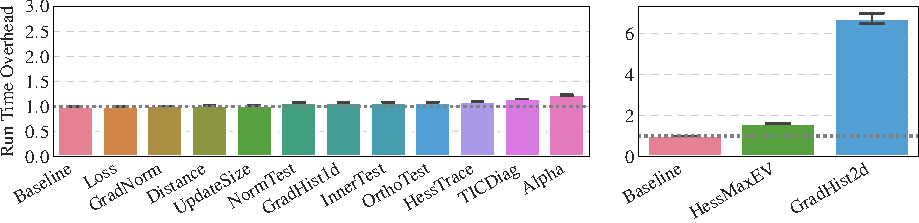
\includegraphics{../repos/cockpit-paper/fig/01_benchmark/output/fig_individual/benchmark_combined_mnist_logreg_cuda_thesis-wide}
    \label{cockpit::fig:app_benchmark_instruments_cuda-mnist_logreg}
  \end{subfigure}
  \vfill
  \begin{subfigure}[t]{\linewidth}
    \caption{Computational overhead for \mnist \mlp (GPU)}
    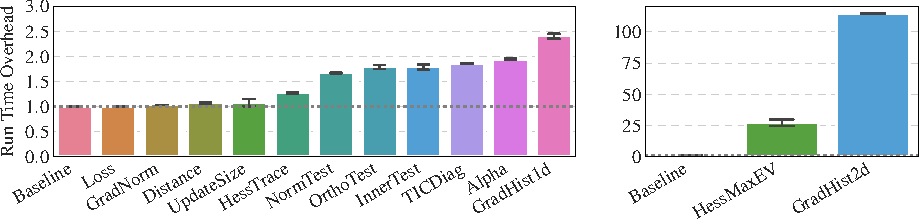
\includegraphics{../repos/cockpit-paper/fig/01_benchmark/output/fig_individual/benchmark_combined_mnist_mlp_cuda_thesis-wide}
    \label{cockpit::fig:app_benchmark_instruments_cuda-mnist_mlp}
  \end{subfigure}
  \vfill
  \begin{subfigure}[t]{\linewidth}
    \caption{Computational overhead for \cifarten \threecthreed (GPU)}
    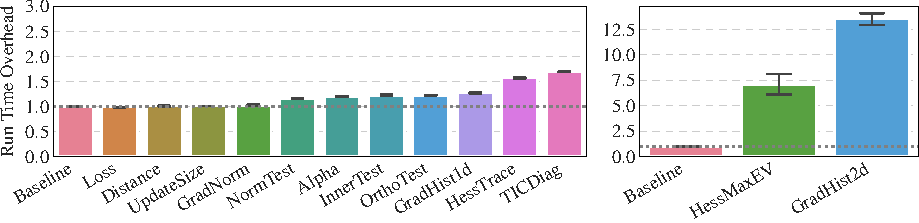
\includegraphics{../repos/cockpit-paper/fig/01_benchmark/output/fig_individual/benchmark_combined_cifar10_3c3d_cuda_thesis-wide}
    \label{cockpit::fig:app_benchmark_instruments_cuda-cifar10}
  \end{subfigure}
  \vfill
  \begin{subfigure}[t]{\linewidth}
    \caption{Computational overhead for \fmnist \twoctwod (GPU)}
    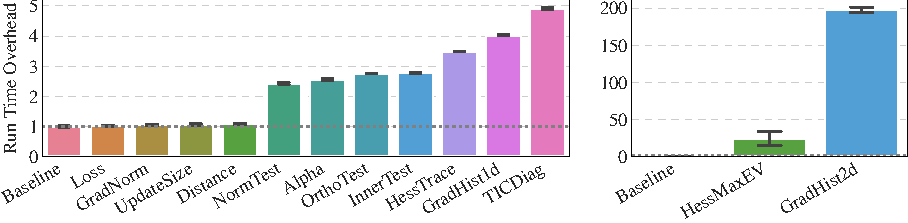
\includegraphics{../repos/cockpit-paper/fig/01_benchmark/output/fig_individual/benchmark_combined_fmnist_2c2d_cuda_thesis-wide}
    \label{cockpit::fig:app_benchmark_instruments_cuda-fmnist}
  \end{subfigure}
  \vfill
  \caption{\textbf{Individual overhead of \cockpittitle's instruments on GPU for
      four different problems.} All run times are shown as multiples of the
    \emph{baseline} without tracking. Expensive quantities are displayed in
    separate panels on the right. Experimental details in the text.}
  \label{cockpit::fig:app_benchmark_instruments_cuda}
\end{figure*}

\captionsetup[subfigure]{justification=centering, singlelinecheck=true}

%%% Local Variables:
%%% mode: latex
%%% TeX-master: "../../../thesis"
%%% End:


\captionsetup[subfigure]{justification=justified,singlelinecheck=false}

\begin{figure*}[p]
  \vfill
  \begin{subfigure}[t]{\linewidth}
    \caption{Computational overhead for \mnist \MNISTNET (CPU)}
    \includegraphics{../repos/cockpit-paper/fig/01_benchmark/output/fig_individual/benchmark_combined_mnist_logreg_cpu_thesis-wide}
    \label{cockpit::fig:app_benchmark_instruments_cpu-mnist_logreg}
  \end{subfigure}
  \vfill
  \begin{subfigure}[t]{\linewidth}
    \caption{Computational overhead for \mnist \mlp (CPU)}
    \includegraphics{../repos/cockpit-paper/fig/01_benchmark/output/fig_individual/benchmark_combined_mnist_mlp_cpu_thesis-wide}
    \label{cockpit::fig:app_benchmark_instruments_cpu-mnist_mlp}
  \end{subfigure}
  \vfill
  \begin{subfigure}[t]{\linewidth}
    \caption{Computational overhead for \cifarten \threecthreed (CPU)}
    \includegraphics{../repos/cockpit-paper/fig/01_benchmark/output/fig_individual/benchmark_combined_cifar10_3c3d_cpu_thesis-wide}
    \label{cockpit::fig:app_benchmark_instruments_cpu-cifar10}
  \end{subfigure}
  \vfill
  \begin{subfigure}[t]{\linewidth}
    \caption{Computational overhead for \fmnist \twoctwod (CPU)}
    \includegraphics{../repos/cockpit-paper/fig/01_benchmark/output/fig_individual/benchmark_combined_fmnist_2c2d_cpu_thesis-wide}
    \label{cockpit::fig:app_benchmark_instruments_cpu-fmnist}
  \end{subfigure}
  \vfill
  \caption{\textbf{Individual overhead of \cockpittitle's instruments on CPU for
      four different problems.} All run times are shown as multiples of the
    \emph{baseline} without tracking. Expensive quantities are displayed in
    separate panels on the right. Experimental details in the text.}
  \label{cockpit::fig:app_benchmark_instruments_cpu}
\end{figure*}

\captionsetup[subfigure]{justification=centering, singlelinecheck=true}

%%% Local Variables:
%%% mode: latex
%%% TeX-master: "../../../thesis"
%%% End:


%%% Local Variables:
%%% mode: latex
%%% TeX-master: "../thesis"
%%% End:

\subsubsection{Configuration Overhead}\label{cockpit::app:benchmark-configuration}

For the estimation of different \cockpit configuration overheads, we use almost
the same setting as described above, training for $512$ iterations and tracking
only every specified interval.

\subsubsection{Configuration Overhead on GPU Versus CPU}

\Cref{cockpit::fig:app_benchmark_configurations_cuda} and
\Cref{cockpit::fig:app_benchmark_configurations_cpu} show the configuration
overhead for four different \deepobs problems. The bottom left part of
\Cref{cockpit::fig:app_benchmark_configurations_cuda} corresponds to
\Cref{cockpit::fig:benchmark_heatmap}. In general, increased parallelism can be
exploited on a GPU, leading to smaller overheads in comparison to a CPU.

\cockpit can even scale to significantly larger problems, such as a \resnetfifty
on \imagenet-like data.
\Cref{cockpit::fig:app_benchmark_configurations_gpu_imagenet} shows the
computational overhead for different tracking intervals on such a large-scale
problem. Using the \textit{economy} configuration, we can achieve our
self-imposed goal of at most doubling the run time even when tracking every
fourth step. More extensive configurations (such as the \textit{full} set) would
indeed have almost prohibitively large costs associated. However, these costs
could be dramatically reduced when one decides to only inspect a part of the
network using \cockpit. Note, individual gradients are not properly defined when
using batch norm, therefore, we replaced these batch norm layers with identity
layers when using the \resnetfifty.

\captionsetup[subfigure]{justification=justified,singlelinecheck=false}

\begin{figure*}[t]
  \centering
  \begin{subfigure}[t]{0.35\linewidth}
    \centering
    \caption{\mnist \MNISTNET (GPU)}
    \includegraphics{../repos/cockpit-paper/fig/01_benchmark/output/fig_grid/benchmark_mnist_logreg_cuda_app_thesis-wide}
    \label{cockpit::fig:app_benchmark_configurations_cuda-mnist_logreg}
  \end{subfigure}
  \hspace{0.1\linewidth}
  \begin{subfigure}[t]{0.35\linewidth}
    \centering
    \caption{\mnist \mlp (GPU)}
    \includegraphics{../repos/cockpit-paper/fig/01_benchmark/output/fig_grid/benchmark_mnist_mlp_cuda_app_thesis-wide}
    \label{cockpit::fig:app_benchmark_configurations_cuda-mnist_mlp}
  \end{subfigure}
  \begin{subfigure}[t]{0.35\linewidth}
    \centering
    \caption{\cifarten \threecthreed (GPU)}
    \includegraphics{../repos/cockpit-paper/fig/01_benchmark/output/fig_grid/benchmark_cifar10_3c3d_cuda_app_thesis-wide}
    \label{cockpit::fig:app_benchmark_configurations_cuda-cifar}
  \end{subfigure}
  \hspace{0.1\linewidth}
  \begin{subfigure}[t]{0.35\linewidth}
    \centering
    \caption{\fmnist \twoctwod (GPU)}
    \includegraphics{../repos/cockpit-paper/fig/01_benchmark/output/fig_grid/benchmark_fmnist_2c2d_cuda_app_thesis-wide}
    \label{cockpit::fig:app_benchmark_configurations_cuda-fmnist}
  \end{subfigure}
  \caption{\textbf{Overhead of \cockpittitle configurations on GPU for four
      different problems with varying tracking interval.} Color bar is the same
    as in \autoref{cockpit::fig:benchmark}.}
  \label{cockpit::fig:app_benchmark_configurations_cuda}
\end{figure*}

\captionsetup[subfigure]{justification=centering, singlelinecheck=true}

%%% Local Variables:
%%% mode: latex
%%% TeX-master: "../../../thesis"
%%% End:


\captionsetup[subfigure]{justification=justified,singlelinecheck=false}

\begin{figure}[t]
	\centering
	\begin{subfigure}[t]{0.4\textwidth}
		\caption{\mnist Log.\,Reg.\,(CPU)}
		\includegraphics[width=\linewidth]{fig/01_benchmark/fig_grid/benchmark_mnist_logreg_cpu_app}
		\label{fig:app_benchmark_configurations_cpu-mnist_logreg}
	\end{subfigure}
	\hspace{0.06\textwidth}
	\begin{subfigure}[t]{0.4\textwidth}
		\caption{\mnist \mlp\,(CPU)}
		\includegraphics[width=\linewidth]{fig/01_benchmark/fig_grid/benchmark_mnist_mlp_cpu_app}
		\label{fig:app_benchmark_configurations_cpu-mnist_mlp}
		\vspace{0.25cm}
	\end{subfigure}
	\begin{subfigure}[t]{0.4\textwidth}
		\caption{\cifarten \threecthreed\,(CPU)}
		\includegraphics[width=\linewidth]{fig/01_benchmark/fig_grid/benchmark_cifar10_3c3d_cpu_app}
		\label{fig:app_benchmark_configurations_cpu-cifar}
	\end{subfigure}
	\hspace{0.06\textwidth}
	\begin{subfigure}[t]{0.4\textwidth}
		\caption{\fmnist \twoctwod\,(GPU)}
		\includegraphics[width=\linewidth]{fig/01_benchmark/fig_grid/benchmark_fmnist_2c2d_cpu_app}
		\label{fig:app_benchmark_configurations_cpu-fmnist}
	\end{subfigure}
	\caption{\textbf{Overhead of \cockpittitle configurations on CPU for four
			different problems with varying tracking interval.} Color bar is the same as in \autoref{fig:benchmark}.}
	\label{fig:app_benchmark_configurations_cpu}
\end{figure}

\captionsetup[subfigure]{justification=centering, singlelinecheck=true}

%%% Local Variables:
%%% mode: latex
%%% TeX-master: "../cockpit_paper"
%%% End:


\clearpage

\begin{figure}[t]
	\centering
	\includegraphics[width=0.59\linewidth]{fig/01_benchmark/fig_grid/benchmark_dummyimagenet_resnet50nobn_cuda_app}
	
	\caption{\textbf{Overhead of \cockpittitle configurations on GPU for \resnetfifty on
			\imagenet.} \cockpit's instruments scale efficiently even to very large problems
			(here: $1000$ classes, $(3, 224, 224)$-sized inputs, and a batch size of $64$.
			For individual gradients to be defined, we replaced the batch norm layers of the 
			\resnetfifty model with identities.) Color bar is the same as in \autoref{fig:benchmark}.}
	\label{fig:app_benchmark_configurations_gpu_imagenet}
\end{figure}


%%% Local Variables:
%%% mode: latex
%%% TeX-master: "../cockpit_paper"
%%% End:


%%% Local Variables:
%%% mode: latex
%%% TeX-master: "../thesis"
%%% End:

\subsection{Performance of Two-dimensional Histograms}\label{cockpit::app:histograms}

Both one- and two-dimensional histograms require $|\sB| \times D$ elements be
accessed, and hence perform similarly. However, we observed different behavior
on GPU and decided to omit the two-dimensional histogram's run time in the main
text. As explained here, this performance lack is not fundamental, but a
shortcoming of the GPU implementation. \pytorch provides built-in functionality
for computing one-dimensional histograms at the time of writing, but is not yet
featuring multi-dimensional histograms. We experimented with three
implementations:
\begin{itemize}
\item \textbf{\pytorch (third party):} A third party
  implementation\footnote{Permission granted by the authors of
    \href{cockpit::https://github.com/miranov25/RootInteractive/blob/7019e4c2b9f291551aeeb8677a969cfcfde690d1/RootInteractive/Tools/Histograms/histogramdd_pytorch.py}{\texttt{github.com/miranov25/.../histogramdd\_pytorch.py}}.}
  under review for being integrated into \pytorch\footnote{See
    \url{https://github.com/pytorch/pytorch/pull/44485}.}. It relies on
  \texttt{torch.bincount}, which uses \inlinecode{atomicAdd}s that represent a
  bottleneck for histograms where most counts are contained in one
  bin.\footnote{See
    \mbox{\url{https://discuss.pytorch.org/t/torch-bincount-1000x-slower-on-cuda/42654}}}
  This occurs often for over-parameterized deep models, as most of the gradient
  elements are zero.

\item \textbf{\pytorch (\cockpittitle):} Our implementation uses a workaround,
  computes bin indices and scatters the counts into their associated bins with
  \inlinecode{torch.Tensor.put\_}. This circumvents \inlinecode{atomicAdd}s, but
  has poor memory locality.

\item \textbf{\numpy:} The single-threaded \inlinecode{numpy.histogram2d} serves
  as baseline, but does not run on GPUs.
\end{itemize}


% pgfplots style "histogrambenchmarkdefault"
\pgfkeys{/pgfplots/histogrambenchmarkdefault/.style={
    enlarge x limits=-0.05,
    width=1.0\linewidth,
    height=0.7\linewidth,
    every axis plot/.append style={line width = 1.5pt},
    tick pos = left,
    ylabel near ticks,
    xlabel near ticks,
    xtick align = inside,
    ytick align = inside,
    legend cell align = left,
    legend columns = 1,
    % legend pos = south east,
    legend style = {
      fill opacity = 0.7,
      text opacity = 1,
      font = \footnotesize,
    },
    xticklabel style = {font = \footnotesize, inner xsep = -5ex},
    xlabel style = {font = \footnotesize},
    axis line style = {black},
    yticklabel style = {font = \footnotesize, inner ysep = -4ex},
    ylabel style = {font = \footnotesize},
    title style = {font = \footnotesize, inner ysep = -3ex},
    grid = major,
    grid style = {dashed}
  }
}

\begin{figure*}
  \begin{subfigure}[t]{0.49\linewidth}
    \pgfkeys{/pgfplots/zmystyle/.style={histogrambenchmarkdefault,
        xlabel={Histogram Balance $b$}
      }}
    \caption{GPU}
    \tikzexternalenable
    % This file was created by tikzplotlib v0.9.3.
\begin{tikzpicture}

\definecolor{color0}{rgb}{0.12156862745098,0.466666666666667,0.705882352941177}
\definecolor{color1}{rgb}{1,0.498039215686275,0.0549019607843137}

\begin{axis}[
axis line style={white!80!black},
legend style={fill opacity=0.8, draw opacity=1, text opacity=1, draw=white!80!black},
tick pos=left,
xlabel={Histogram Balance},
xmin=-0.039, xmax=1.039,
ylabel={Run Time [s]},
ymin=0.0647793941403482, ymax=344.025767453251,
ymode=log,
zmystyle
]
\addplot [, color0, dashed]
table {%
0.01 4.54533004760742
0.0615789473684211 2.08099224567413
0.113157894736842 0.744264936447144
0.164736842105263 0.445815587043762
0.216315789473684 0.335660696029663
0.267894736842105 0.282471227645874
0.319473684210526 0.253187036514282
0.371052631578947 0.232630848884583
0.422631578947368 0.219761872291565
0.474210526315789 0.210704207420349
0.52578947368421 0.206429862976074
0.577368421052632 0.218602991104126
0.628947368421053 0.214805579185486
0.680526315789474 0.20776104927063
0.732105263157895 0.20455629825592
0.783684210526316 0.20727813243866
0.835263157894737 0.206504940986633
0.886842105263158 0.203398704528809
0.9 0.20402295589447
0.938421052631579 0.204293870925903
0.99 0.204171013832092
};
\addlegendentry{\textsc{PyTorch} (\textsc{Cockpit})}
\addplot [, color1, dashed]
table {%
0.01 232.951647591591
0.0615789473684211 67.0944833517075
0.113157894736842 12.7715488433838
0.164736842105263 5.53443562984467
0.216315789473684 2.58965411186218
0.267894736842105 1.4656699180603
0.319473684210526 0.907050752639771
0.371052631578947 0.633884406089783
0.422631578947368 0.44161102771759
0.474210526315789 0.332058143615723
0.52578947368421 0.243267822265625
0.577368421052632 0.193850588798523
0.628947368421053 0.160495829582214
0.680526315789474 0.137686920166016
0.732105263157895 0.118721318244934
0.783684210526316 0.105425000190735
0.835263157894737 0.106805515289307
0.886842105263158 0.108340263366699
0.9 0.105959153175354
0.938421052631579 0.103169775009155
0.99 0.0956669807434082
};
\addlegendentry{\textsc{PyTorch} (third party)}
\end{axis}

\end{tikzpicture}

    \tikzexternaldisable
    \label{cockpit::fig:app-histogram2d-benchmark-gpu}
  \end{subfigure}
  \hfill
  \begin{subfigure}[t]{0.49\linewidth}
    \pgfkeys{/pgfplots/zmystyle/.style={histogrambenchmarkdefault,
        xlabel={Histogram Balance $b$}
      }}
    \caption{CPU}
    \tikzexternalenable
    % This file was created by tikzplotlib v0.9.3.
\begin{tikzpicture}

\definecolor{color0}{rgb}{0.12156862745098,0.466666666666667,0.705882352941177}
\definecolor{color1}{rgb}{1,0.498039215686275,0.0549019607843137}
\definecolor{color2}{rgb}{0.172549019607843,0.627450980392157,0.172549019607843}

\begin{axis}[
axis line style={white!80!black},
legend style={fill opacity=0.8, draw opacity=1, text opacity=1, at={(0.91,0.5)}, anchor=east, draw=white!80!black},
tick pos=left,
xlabel={Histogram Balance},
xmin=-0.039, xmax=1.039,
ylabel={Run Time [s]},
ymin=0.919387552518064, ymax=8.28341609861724,
ymode=log,
zmystyle
]
\addplot [, color0, dashed]
table {%
0.01 1.04204399585724
0.0615789473684211 1.03900332450867
0.113157894736842 1.07859117984772
0.164736842105263 1.06876609325409
0.216315789473684 1.04880547523499
0.267894736842105 1.04529702663422
0.319473684210526 1.05313646793365
0.371052631578947 1.06466472148895
0.422631578947368 1.06266655921936
0.474210526315789 1.05389556884766
0.52578947368421 1.06146202087402
0.577368421052632 1.04773416519165
0.628947368421053 1.06101129055023
0.680526315789474 1.04648265838623
0.732105263157895 1.0483683347702
0.783684210526316 1.04395830631256
0.835263157894737 1.04497628211975
0.886842105263158 1.04231572151184
0.9 1.04766194820404
0.938421052631579 1.04687905311584
0.99 1.0437038898468
};
\addlegendentry{\textsc{PyTorch} (\textsc{Cockpit})}
\addplot [, color1, dashed]
table {%
0.01 1.02336490154266
0.0615789473684211 1.02175369262695
0.113157894736842 1.02237765789032
0.164736842105263 1.02118575572968
0.216315789473684 1.01996810436249
0.267894736842105 1.02348549365997
0.319473684210526 1.0248743057251
0.371052631578947 1.02083847522736
0.422631578947368 1.01863925457001
0.474210526315789 1.02599215507507
0.52578947368421 1.0236154794693
0.577368421052632 1.02260437011719
0.628947368421053 1.03915128707886
0.680526315789474 1.03184995651245
0.732105263157895 1.0255656003952
0.783684210526316 1.0171329498291
0.835263157894737 1.02414612770081
0.886842105263158 1.02574753761292
0.9 1.01600201129913
0.938421052631579 1.01842267513275
0.99 1.02955875396729
};
\addlegendentry{\textsc{PyTorch} (third party)}
\addplot [, color2, dashed]
table {%
0.01 3.44840505123138
0.0615789473684211 3.95587799549103
0.113157894736842 4.67446537017822
0.164736842105263 4.98263554573059
0.216315789473684 5.3127799987793
0.267894736842105 5.58865821361542
0.319473684210526 5.89873046875
0.371052631578947 6.09700152873993
0.422631578947368 6.21813678741455
0.474210526315789 6.48546359539032
0.52578947368421 6.69456965923309
0.577368421052632 6.80199146270752
0.628947368421053 6.89959270954132
0.680526315789474 7.07993612289429
0.732105263157895 7.23664236068726
0.783684210526316 7.27940900325775
0.835263157894737 7.2930465221405
0.886842105263158 7.35840466022491
0.938421052631579 7.44740259647369
0.99 7.4957230091095
};
\addlegendentry{\textsc{NumPy} (single thread)}
\end{axis}

\end{tikzpicture}

    \tikzexternaldisable
    \label{cockpit::fig:app-histogram2d-benchmark-cpu}
  \end{subfigure}
  \caption{\textbf{Performance of two-dimensional histogram GPU implementations
      depends on the data.} (\subref{cockpit::fig:app-histogram2d-benchmark-gpu}) Run
    time for two different GPU implementations with histograms of different
    imbalance. \cockpit's implementation outperforms the third party solution by
    more than one order of magnitude in the deep learning regime ($b \ll 1$).
    (\subref{cockpit::fig:app-histogram2d-benchmark-cpu}) On CPU, performance is robust
    to histogram balance. The run time difference between \numpy and \pytorch is
    due to multi-threading. Data has the same size as \deepobs's \cifarten
    \threecthreed problem ($D =895,210, |\sB| = 128$). Curves represent averages
    over 10 independent runs. Error bars are omitted to improve legibility.}
  \label{cockpit::fig:app-histogram2d-benchmark}
\end{figure*}

To demonstrate the strong performance dependence on the data, we generate data
from a uniform distribution over $[0, b]\times[0, b]$, where $b \in (0, 1)$
parametrizes the histogram's balance, and compute two-dimensional histograms on
$[0,1]\times [0, 1]$. \Cref{cockpit::fig:app-histogram2d-benchmark-gpu} shows a
clear increase in run time of both GPU implementations for more imbalanced
histograms. Note that even though our implementation outperforms the third party
by more than one order of magnitude in the deep neural network regime ($b \ll
1$), it is still considerably slower than a one-dimensional histogram (see
\Cref{cockpit::fig:app_benchmark_instruments_cuda} (c)), and even slower on GPU
than on CPU (\Cref{cockpit::fig:app-histogram2d-benchmark} (b)). As expected,
the CPU implementations do not significantly depend on the data
(\Cref{cockpit::fig:app-histogram2d-benchmark-cpu}). The performance difference
between \pytorch and \numpy is likely due to multi-threading versus
single-threading.

Although a carefully engineered histogram GPU implementation is currently not
available, we think it will reduce the computational overhead to that of a
one-dimensional histogram in future releases.

%%% Local Variables:
%%% mode: latex
%%% TeX-master: "../thesis"
%%% End:

\clearpage

\section{\cockpittitle View of Convex Stochastic Problems}\label{cockpit::app:convex-problems}
\begin{figure*}[!h]
  \centering \Cshadowbox{\includegraphics[width=.97\linewidth, trim={7cm 2.5cm
      5cm 0.5cm}, clip]{../repos/cockpit-paper/tex/fig/10_showcase/quadratic_deep_log.png}}

  \Cshadowbox{\includegraphics[width=.97\linewidth, trim={7cm 2.5cm 5cm 0.5cm},
    clip]{../repos/cockpit-paper/tex/fig/10_showcase/mnist_logreg_log.png}}

  \vspace{0.5\baselineskip}

  \caption{\textbf{Screenshot of \cockpittitle's full view for convex \deepobs
      problems.} Top \cockpit shows training on a noisy quadratic loss function.
    Bottom shows training on logistic regression on \mnist . Figure and labels
    are not meant to be legible. It is evident, that there is a fundamental
    difference in the optimization process, compared to training deep networks,
    \ie \Cref{cockpit::fig:showcase}. This is, for example, visible when comparing the
    gradient norms, which converge to zero for convex problems but not for deep
    learning.}\label{cockpit::fig:convex-problems}
\end{figure*}

%%% Local Variables:
%%% mode: latex
%%% TeX-master: "../thesis"
%%% End:


%%% Local Variables:
%%% mode: latex
%%% TeX-master: "../thesis"
%%% End:


\setchapterpreamble[u]{\margintoc}
\chapter{Additional Material for Chapter \ref{chap:vivit}}
\section{Mathematical Details}\label{vivit::sec:math-details}
\subsection{The \gnn's Eigenvalues \& the Gram
  Matrix}\label{vivit::sec:relation-ggn-gram-eigenvalues}

For \Cref{vivit::eq:ggn-eigenvalues}, consider the left hand side of the \ggn's
characteristic polynomial $\det(\mG - \lambda \mI_D) = 0$. Inserting the \vivit
factorization (\Cref{vivit::eq:ggn-factorization}) and using the matrix determinant
lemma yields
\begin{align*}
  &\det\left(
  - \lambda \mI_D + \mG
  \right)
  \\
  &\qquad =
    \det\!\left(
    - \lambda \mI_D + \mV\mV^\top
    \right)
    \explainmath{(Low-rank structure (\ref{vivit::eq:ggn-factorization}))}
  \\
  &\qquad=
    \det\!\left(
    \mI_{NC} + \mV^\top (-\lambda \mI_D)^{-1} \mV
    \right)
    \det\!\left(
    -\lambda \mI_D
    \right)
    \explainmath{(Matrix determinant lemma)}
  \\
  &\qquad=
    \det\!\left(
    \mI_{NC} - \frac{1}{\lambda} \mV^\top \mV
    \right)
    (-\lambda)^D
    \explainmath{\empty}
  \\
  &\qquad=
    \left(-\frac{1}{\lambda}\right)^{NC}
    \det\!\left(
    \mV^\top \mV - \lambda \mI_{NC}
    \right)
    (-\lambda)^D
    \explainmath{\empty}
  \\
  &\qquad=
    (-\lambda)^{D - NC}
    \det\!\left(
    \mGtilde - \lambda \mI_{NC}
    \right)\,.
    \explainmath{(Gram matrix)}
\end{align*}
Setting the above expression to zero reveals that the \ggn's spectrum decomposes
into $D-NC$ zero eigenvalues and the Gram matrix spectrum obtained from
$\det(\mGtilde - \lambda \mI_{NC} )= 0$.

\subsection{Relation Between \ggn \& Gram Matrix Eigenvectors}
\label{vivit::sec:relation-ggn-gram-eigenvectors}

Assume the nontrivial Gram matrix spectrum $\tilde{\sS}_+ := \{(\lambda_k,
\vetilde_k)\:|\: \lambda_k \neq 0, \mGtilde \vetilde_k = \lambda_k \vetilde_k
\}_{k=1}^K$ with orthonormal eigenvectors $\vetilde_j^\top \vetilde_k =
\delta_{j,k}$ ($\delta$ is the Kronecker delta) and $K = \mathrm{rank}(\mG)$. We
now show that $\ve_k = \nicefrac{1}{\sqrt{\lambda_k}} \mV \vetilde_k$ are
normalized eigenvectors of $\mG$ and inherit orthogonality from $\vetilde_k$.

To see the first, consider right-multiplication of the \ggn with $\ve_k$, then
expand the low-rank structure,
\begin{align*}
  \mG \ve_k
  &=
    \frac{1}{\sqrt{\lambda_k}}
    \mV \mV^\top  \mV \vetilde_k
    \explainmath{(\Cref{vivit::eq:ggn-factorization} and definition of $\ve_k$)}
  \\
  &=
    \frac{1}{\sqrt{\lambda_k}}
    \mV \mGtilde \vetilde_k
    \explainmath{(Gram matrix)}
  \\
  &=
    \lambda_k\frac{1}{\sqrt{\lambda_k}}
    \mV \vetilde_k
    \explainmath{(Eigenvector property of $\vetilde_k$)}
  \\
  &= \lambda_k \ve_k\,.
\end{align*}
Orthonormality of the $\ve_k$ results from the Gram matrix eigenvector
orthonormality,
\begin{align*}
  \ve_j^\top \ve_{k}
  &=
    \left(
    \frac{1}{\sqrt{\lambda_j}} \vetilde_j^\top \mV ^\top
    \right)
    \left(
    \frac{1}{\sqrt{\lambda_k}} \mV \vetilde_k
    \right)
    \explainmath{(Definition of $\ve_j, \ve_k$)}
  \\
  &=
    \frac{1}{\sqrt{\lambda_j\lambda_k}} \vetilde_j^\top \mGtilde \vetilde_k
    \explainmath{(Gram matrix)}
  \\
  &=
    \frac{\lambda_k}{\sqrt{\lambda_j\lambda_k}} \vetilde_j^\top \vetilde_k
    \explainmath{(Eigenvector property of $\vetilde_k$)}
  \\
  &=
    \delta_{j,k}\,.
    \explainmath{(Orthonormality)}
\end{align*}

%%% Local Variables:
%%% mode: latex
%%% TeX-master: "../thesis"
%%% End:


\section{Experimental Details}\label{vivit::sec:experimental-details}
This section uses the notation from \Cref{vivit::sec:experiments} (see
\Cref{vivit::tab:notation_cases}).

\begin{table}[ht]
  \centering
  \caption{ \textbf{Notation for curvature approximations.} The notation is
    introduced in \Cref{vivit::sec:experiments}. This table recapitulates the
    abbreviations (referring to the approximations introduced in
    \Cref{vivit::sec:approximations}) and provides corresponding explanations. }
  \label{vivit::tab:notation_cases}
  \vspace{1ex}
  \begin{footnotesize}
    \begin{tabular}{ll}
      \toprule
      Abbreviation
      & Explanation \\
      \midrule
      \textbf{mb, exact}
      & \makecell[tl]{Exact \ggn with all mini-batch samples.\\
      Backpropagates $NC$ vectors.}
      \\
      \textbf{mb, mc}
      & \makecell[tl]{ \mc-approximated \ggn with all mini-batch samples.\\
      Backpropagates $N M$ vectors with $M$ the number of \mc{}-samples.}
      \\
      \textbf{sub, exact}
      & \makecell[tl]{Exact \ggn on a subset of mini-batch samples ($\floor{\nicefrac{N}{8}}$ as in \cite{zhang2017blockdiagonal}).\\
      Backpropagates $\floor{\nicefrac{N}{8}} C$ vectors.}
      \\
      \textbf{sub, mc}
      & \makecell[tl]{\mc-approximated \ggn on a subset of mini-batch samples.\\
      Backpropagates $\floor{\nicefrac{N}{8}} M$ vectors with $M$ the number of \mc{}-samples.}
      \\
      \bottomrule
    \end{tabular}
  \end{footnotesize}
\end{table}

%%% Local Variables:
%%% mode: latex
%%% TeX-master: "../thesis"
%%% End:

\subsubsection{\ggn Spectra (\Cref{vivit::subfig:visual-abstract1})}

To obtain the spectra of \Cref{vivit::subfig:visual-abstract1} we initialize the
respective architecture, then draw a mini-batch and evaluate the \ggn
eigenvalues under the described approximations, clipping the Gram matrix
eigenvalues at $10^{-4}$. \Cref{vivit::fig:spectrum_1} provides the spectra for
all used architectures with both the full \ggn and a per-layer block-diagonal
approximation.

\begin{figure*}[p]
  \centering

  \begin{minipage}[t]{0.495\linewidth}
    \centering
    \begin{footnotesize}
      \textbf{Full network}
    \end{footnotesize}
  \end{minipage}
  \hfill
  \begin{minipage}[t]{0.495\linewidth}
    \centering
    \begin{footnotesize}
      \textbf{Block-diagonal approximation}
    \end{footnotesize}
  \end{minipage}

  \begin{subfigure}[t]{\linewidth}
    \centering
    \caption{\fmnist \twoctwod}
    \begin{minipage}[t]{0.495\linewidth}
      \centering
      \begin{minipage}[t]{0.33\linewidth}
        \centering
        % load "spectrumdefault{left, center, right}" styles
        \input{figures/vivit/spectrum_default_style}
        % customize "zmystyle" as you wish
        \pgfkeys{/pgfplots/zmystyle/.style={spectrumdefaultleft,
            title={exact, mb}}}
        \tikzexternalenable
        \input{../repos/vivit-paper/fig/exp10_performance_ggn_evals/fig/evals/fmnist_2c2d_cpu_one_group_full_batch_exact}
        \tikzexternaldisable
      \end{minipage}
      \hspace{1.9ex}
      \begin{minipage}[t]{0.33\linewidth}
        \centering
        % load "spectrumdefault{left, center, right}" styles
        \input{figures/vivit/spectrum_default_style}
        % customize "zmystyle" as you wish
        \pgfkeys{/pgfplots/zmystyle/.style={spectrumdefaultcenter,
            title={exact, sub}}}
        \tikzexternalenable
        \input{../repos/vivit-paper/fig/exp10_performance_ggn_evals/fig/evals/fmnist_2c2d_cpu_one_group_frac_batch_exact}
        \tikzexternaldisable
      \end{minipage}
      \hspace{-3.5ex}
      \begin{minipage}[t]{0.33\linewidth}
        \centering
        % load "spectrumdefault{left, center, right}" styles
        \input{figures/vivit/spectrum_default_style}
        % customize "zmystyle" as you wish
        \pgfkeys{/pgfplots/zmystyle/.style={spectrumdefaultright,
            title={mc, full}}}
        \tikzexternalenable
        \input{../repos/vivit-paper/fig/exp10_performance_ggn_evals/fig/evals/fmnist_2c2d_cpu_one_group_full_batch_mc}
        \tikzexternaldisable
      \end{minipage}
    \end{minipage}
    \hfill
    \begin{minipage}[t]{0.495\linewidth}
      \centering
      \begin{minipage}[t]{0.33\linewidth}
        \centering
        % load "spectrumdefault{left, center, right}" styles
        \input{figures/vivit/spectrum_default_style}
        % customize "zmystyle" as you wish
        \pgfkeys{/pgfplots/zmystyle/.style={spectrumdefaultleft, ymax = 5e-4,
            title={exact, mb}}}
        \tikzexternalenable
        \input{../repos/vivit-paper/fig/exp10_performance_ggn_evals/fig/evals/fmnist_2c2d_cpu_layerwise_group_full_batch_exact}
        \tikzexternaldisable
      \end{minipage}
      \hspace{1.9ex}
      \begin{minipage}[t]{0.33\linewidth}
        \centering
        % load "spectrumdefault{left, center, right}" styles
        \input{figures/vivit/spectrum_default_style}
        % customize "zmystyle" as you wish
        \pgfkeys{/pgfplots/zmystyle/.style={spectrumdefaultcenter, ymax = 5e-4,
            title={exact, sub}}}
        \tikzexternalenable
        \input{../repos/vivit-paper/fig/exp10_performance_ggn_evals/fig/evals/fmnist_2c2d_cpu_layerwise_group_frac_batch_exact}
        \tikzexternaldisable
      \end{minipage}
      \hspace{-3.5ex}
      \begin{minipage}[t]{0.33\linewidth}
        \centering
        % load "spectrumdefault{left, center, right}" styles
        \input{figures/vivit/spectrum_default_style}
        % customize "zmystyle" as you wish
        \pgfkeys{/pgfplots/zmystyle/.style={spectrumdefaultright, ymax = 5e-4,
            title={mc, full}}}
        \tikzexternalenable
        \input{../repos/vivit-paper/fig/exp10_performance_ggn_evals/fig/evals/fmnist_2c2d_cpu_layerwise_group_full_batch_mc}
        \tikzexternaldisable
      \end{minipage}
    \end{minipage}
  \end{subfigure}

  \begin{subfigure}{\linewidth}
    \centering
    \caption{\cifarten \threecthreed}
    \begin{minipage}{0.495\linewidth}
      \centering
      \begin{minipage}[t]{0.33\linewidth}
        \centering
        % load "spectrumdefault{left, center, right}" styles
        \input{figures/vivit/spectrum_default_style}
        % customize "zmystyle" as you wish
        \pgfkeys{/pgfplots/zmystyle/.style={spectrumdefaultleft,
            title={exact, mb}}}
        \tikzexternalenable
        \input{../repos/vivit-paper/fig/exp10_performance_ggn_evals/fig/evals/cifar10_3c3d_cpu_one_group_full_batch_exact}
        \tikzexternaldisable
      \end{minipage}
      \hspace{1.9ex}
      \begin{minipage}[t]{0.33\linewidth}
        \centering
        % load "spectrumdefault{left, center, right}" styles
        \input{figures/vivit/spectrum_default_style}
        % customize "zmystyle" as you wish
        \pgfkeys{/pgfplots/zmystyle/.style={spectrumdefaultcenter,
            title={exact, sub}}}
        \tikzexternalenable
        \input{../repos/vivit-paper/fig/exp10_performance_ggn_evals/fig/evals/cifar10_3c3d_cpu_one_group_frac_batch_exact}
        \tikzexternaldisable
      \end{minipage}
      \hspace{-3.5ex}
      \begin{minipage}[t]{0.33\linewidth}
        \centering
        % load "spectrumdefault{left, center, right}" styles
        \input{figures/vivit/spectrum_default_style}
        % customize "zmystyle" as you wish
        \pgfkeys{/pgfplots/zmystyle/.style={spectrumdefaultright,
            title={mc, full}}}
        \tikzexternalenable
        \input{../repos/vivit-paper/fig/exp10_performance_ggn_evals/fig/evals/cifar10_3c3d_cpu_one_group_full_batch_mc}
        \tikzexternaldisable
      \end{minipage}
    \end{minipage}
    \hfill
    \begin{minipage}{0.495\linewidth}
      \centering
      \begin{minipage}[t]{0.33\linewidth}
        \centering
        % load "spectrumdefault{left, center, right}" styles
        \input{figures/vivit/spectrum_default_style}
        % customize "zmystyle" as you wish
        \pgfkeys{/pgfplots/zmystyle/.style={spectrumdefaultleft, ymax = 3e-3,
            title={exact, mb}}}
        \tikzexternalenable
        \input{../repos/vivit-paper/fig/exp10_performance_ggn_evals/fig/evals/cifar10_3c3d_cpu_layerwise_group_full_batch_exact}
        \tikzexternaldisable
      \end{minipage}
      \hspace{1.9ex}
      \begin{minipage}[t]{0.33\linewidth}
        \centering
        % load "spectrumdefault{left, center, right}" styles
        \input{figures/vivit/spectrum_default_style}
        % customize "zmystyle" as you wish
        \pgfkeys{/pgfplots/zmystyle/.style={spectrumdefaultcenter, ymax = 3e-3,
            title={exact, sub}}}
        \tikzexternalenable
        \input{../repos/vivit-paper/fig/exp10_performance_ggn_evals/fig/evals/cifar10_3c3d_cpu_layerwise_group_frac_batch_exact}
        \tikzexternaldisable
      \end{minipage}
      \hspace{-3.5ex}
      \begin{minipage}[t]{0.33\linewidth}
        \centering
        % load "spectrumdefault{left, center, right}" styles
        \input{figures/vivit/spectrum_default_style}
        % customize "zmystyle" as you wish
        \pgfkeys{/pgfplots/zmystyle/.style={spectrumdefaultright, ymax = 3e-3,
            title={mc, full}}}
        \tikzexternalenable
        \input{../repos/vivit-paper/fig/exp10_performance_ggn_evals/fig/evals/cifar10_3c3d_cpu_layerwise_group_full_batch_mc}
        \tikzexternaldisable
      \end{minipage}
    \end{minipage}
  \end{subfigure}

  \begin{subfigure}[t]{\linewidth}
    \centering
    \caption{\cifarten \resnetthirtytwo}
    \begin{minipage}{0.495\linewidth}
      \centering
      \begin{minipage}[t]{0.33\linewidth}
        \centering
        % load "spectrumdefault{left, center, right}" styles
        \input{figures/vivit/spectrum_default_style}
        % customize "zmystyle" as you wish
        \pgfkeys{/pgfplots/zmystyle/.style={spectrumdefaultleft, ymax = 1e-4,
            title={exact, mb}}}
        \tikzexternalenable
        \input{../repos/vivit-paper/fig/exp10_performance_ggn_evals/fig/evals/cifar10_resnet32_cpu_one_group_full_batch_exact}
        \tikzexternaldisable
      \end{minipage}
      \hspace{1.9ex}
      \begin{minipage}[t]{0.33\linewidth}
        \centering
        % load "spectrumdefault{left, center, right}" styles
        \input{figures/vivit/spectrum_default_style}
        % customize "zmystyle" as you wish
        \pgfkeys{/pgfplots/zmystyle/.style={spectrumdefaultcenter, ymax = 1e-4,
            title={exact, sub}}}
        \tikzexternalenable
        \input{../repos/vivit-paper/fig/exp10_performance_ggn_evals/fig/evals/cifar10_resnet32_cpu_one_group_frac_batch_exact}
        \tikzexternaldisable
      \end{minipage}
      \hspace{-3.5ex}
      \begin{minipage}[t]{0.33\linewidth}
        \centering
        % load "spectrumdefault{left, center, right}" styles
        \input{figures/vivit/spectrum_default_style}
        % customize "zmystyle" as you wish
        \pgfkeys{/pgfplots/zmystyle/.style={spectrumdefaultright, ymax = 1e-4,
            title={mc, full}}}
        \tikzexternalenable
        \input{../repos/vivit-paper/fig/exp10_performance_ggn_evals/fig/evals/cifar10_resnet32_cpu_one_group_full_batch_mc}
        \tikzexternaldisable
      \end{minipage}
    \end{minipage}
    \begin{minipage}{0.495\linewidth}
      \centering
      \begin{minipage}[t]{0.33\linewidth}
        \centering
        % load "spectrumdefault{left, center, right}" styles
        \input{figures/vivit/spectrum_default_style}
        % customize "zmystyle" as you wish
        \pgfkeys{/pgfplots/zmystyle/.style={spectrumdefaultleft, ymax = 3e-3,
            title={exact, mb}}}
        \tikzexternalenable
        \input{../repos/vivit-paper/fig/exp10_performance_ggn_evals/fig/evals/cifar10_resnet32_cpu_layerwise_group_full_batch_exact}
        \tikzexternaldisable
      \end{minipage}
      \hspace{1.9ex}
      \begin{minipage}[t]{0.33\linewidth}
        \centering
        % load "spectrumdefault{left, center, right}" styles
        \input{figures/vivit/spectrum_default_style}
        % customize "zmystyle" as you wish
        \pgfkeys{/pgfplots/zmystyle/.style={spectrumdefaultcenter, ymax = 3e-3,
            title={exact, sub}}}
        \tikzexternalenable
        \input{../repos/vivit-paper/fig/exp10_performance_ggn_evals/fig/evals/cifar10_resnet32_cpu_layerwise_group_frac_batch_exact}
        \tikzexternaldisable
      \end{minipage}
      \hspace{-3.5ex}
      \begin{minipage}[t]{0.33\linewidth}
        \centering
        % load "spectrumdefault{left, center, right}" styles
        \input{figures/vivit/spectrum_default_style}
        % customize "zmystyle" as you wish
        \pgfkeys{/pgfplots/zmystyle/.style={spectrumdefaultright, ymax = 3e-3,
            title={mc, full}}}
        \tikzexternalenable
        \input{../repos/vivit-paper/fig/exp10_performance_ggn_evals/fig/evals/cifar10_resnet32_cpu_layerwise_group_full_batch_mc}
        \tikzexternaldisable
      \end{minipage}
    \end{minipage}
  \end{subfigure}
  \caption{\textbf{\ggn spectra of different architectures under \vivittitle's
      approximations:} Left and right columns contain results with the full
    network's \ggn and a per-layer block-diagonal approximation,
    respectively.} \label{vivit::fig:spectrum_1}
\end{figure*}

\addtocounter{figure}{-1}

\begin{figure*}[!t]
  \centering
  \begin{minipage}[t]{0.495\linewidth}
    \centering
    \begin{footnotesize}
      \textbf{Full network}
    \end{footnotesize}
  \end{minipage}
  \hfill
  \begin{minipage}[t]{0.495\linewidth}
    \centering
    \begin{footnotesize}
      \textbf{Block-diagonal approximation}
    \end{footnotesize}
  \end{minipage}

  \begin{subfigure}[t]{\linewidth}
    \addtocounter{subfigure}{3}
    \caption{\cifarten \resnetfiftysix}
    \centering
    \begin{minipage}{0.495\linewidth}
      \centering
      \begin{minipage}[t]{0.33\linewidth}
        \centering
        % load "spectrumdefault{left, center, right}" styles
        \input{figures/vivit/spectrum_default_style}
        % customize "zmystyle" as you wish
        \pgfkeys{/pgfplots/zmystyle/.style={spectrumdefaultleft, ymax = 1e-4,
            title={exact, mb}}}
        \tikzexternalenable
        \input{../repos/vivit-paper/fig/exp10_performance_ggn_evals/fig/evals/cifar10_resnet56_cpu_one_group_full_batch_exact}
        \tikzexternaldisable
      \end{minipage}
      \hspace{1.9ex}
      \begin{minipage}[t]{0.33\linewidth}
        \centering
        % load "spectrumdefault{left, center, right}" styles
        \input{figures/vivit/spectrum_default_style}
        % customize "zmystyle" as you wish
        \pgfkeys{/pgfplots/zmystyle/.style={spectrumdefaultcenter, ymax = 1e-4,
            title={exact, sub}}}
        \tikzexternalenable
        \input{../repos/vivit-paper/fig/exp10_performance_ggn_evals/fig/evals/cifar10_resnet56_cpu_one_group_frac_batch_exact}
        \tikzexternaldisable
      \end{minipage}
      \hspace{-3.5ex}
      \begin{minipage}[t]{0.33\linewidth}
        \centering
        % load "spectrumdefault{left, center, right}" styles
        \input{figures/vivit/spectrum_default_style}
        % customize "zmystyle" as you wish
        \pgfkeys{/pgfplots/zmystyle/.style={spectrumdefaultright, ymax = 1e-4,
            title={mc, full}}}
        \tikzexternalenable
        \input{../repos/vivit-paper/fig/exp10_performance_ggn_evals/fig/evals/cifar10_resnet56_cpu_one_group_full_batch_mc}
        \tikzexternaldisable
      \end{minipage}
    \end{minipage}
    \hfill
    \begin{minipage}{0.495\linewidth}
      \centering
      \begin{minipage}[t]{0.33\linewidth}
        \centering
        % load "spectrumdefault{left, center, right}" styles
        \input{figures/vivit/spectrum_default_style}
        % customize "zmystyle" as you wish
        \pgfkeys{/pgfplots/zmystyle/.style={spectrumdefaultleft, ymax = 3e-3,
            title={exact, mb}}}
        \tikzexternalenable
        \input{../repos/vivit-paper/fig/exp10_performance_ggn_evals/fig/evals/cifar10_resnet56_cpu_layerwise_group_full_batch_exact}
        \tikzexternaldisable
      \end{minipage}
      \hspace{1.9ex}
      \begin{minipage}[t]{0.33\linewidth}
        \centering
        % load "spectrumdefault{left, center, right}" styles
        \input{figures/vivit/spectrum_default_style}
        % customize "zmystyle" as you wish
        \pgfkeys{/pgfplots/zmystyle/.style={spectrumdefaultcenter, ymax = 3e-3,
            title={exact, sub}}}
        \tikzexternalenable
        \input{../repos/vivit-paper/fig/exp10_performance_ggn_evals/fig/evals/cifar10_resnet56_cpu_layerwise_group_frac_batch_exact}
        \tikzexternaldisable
      \end{minipage}
      \hspace{-3.5ex}
      \begin{minipage}[t]{0.33\linewidth}
        \centering
        % load "spectrumdefault{left, center, right}" styles
        \input{figures/vivit/spectrum_default_style}
        % customize "zmystyle" as you wish
        \pgfkeys{/pgfplots/zmystyle/.style={spectrumdefaultright, ymax = 3e-3,
            title={mc, full}}}
        \tikzexternalenable
        \input{../repos/vivit-paper/fig/exp10_performance_ggn_evals/fig/evals/cifar10_resnet56_cpu_layerwise_group_full_batch_mc}
        \tikzexternaldisable
      \end{minipage}
    \end{minipage}
  \end{subfigure}

  \begin{subfigure}[t]{\linewidth}
    \centering
    \caption{\cifarhun \allcnnc}
    \begin{minipage}{0.495\linewidth}
      \centering
      \begin{minipage}[t]{0.33\linewidth}
        \centering
        % load "spectrumdefault{left, center, right}" styles
        \input{figures/vivit/spectrum_default_style}
        % customize "zmystyle" as you wish
        \pgfkeys{/pgfplots/zmystyle/.style={spectrumdefaultleft, ymax = 1e-3,
            title={exact, mb}}}
        \tikzexternalenable
        \input{../repos/vivit-paper/fig/exp10_performance_ggn_evals/fig/evals/cifar100_allcnnc_cpu_one_group_full_batch_exact}
        \tikzexternaldisable
      \end{minipage}
      \hspace{1.9ex}
      \begin{minipage}[t]{0.33\linewidth}
        \centering
        % load "spectrumdefault{left, center, right}" styles
        \input{figures/vivit/spectrum_default_style}
        % customize "zmystyle" as you wish
        \pgfkeys{/pgfplots/zmystyle/.style={spectrumdefaultcenter, ymax = 1e-3,
            title={exact, sub}}}
        \tikzexternalenable
        \input{../repos/vivit-paper/fig/exp10_performance_ggn_evals/fig/evals/cifar100_allcnnc_cpu_one_group_frac_batch_exact}
        \tikzexternaldisable
      \end{minipage}
      \hspace{-3.5ex}
      \begin{minipage}[t]{0.33\linewidth}
        \centering
        % load "spectrumdefault{left, center, right}" styles
        \input{figures/vivit/spectrum_default_style}
        % customize "zmystyle" as you wish
        \pgfkeys{/pgfplots/zmystyle/.style={spectrumdefaultright, ymax = 1e-3,
            title={mc, full}}}
        \tikzexternalenable
        \input{../repos/vivit-paper/fig/exp10_performance_ggn_evals/fig/evals/cifar100_allcnnc_cpu_one_group_full_batch_mc}
        \tikzexternaldisable
      \end{minipage}
    \end{minipage}
    \hfill
    \begin{minipage}{0.495\linewidth}
      \centering
      \begin{minipage}[t]{0.33\linewidth}
        \centering
        % load "spectrumdefault{left, center, right}" styles
        \input{figures/vivit/spectrum_default_style}
        % customize "zmystyle" as you wish
        \pgfkeys{/pgfplots/zmystyle/.style={spectrumdefaultleft, ymax = 5e-3,
            title={exact, mb}}}
        \tikzexternalenable
        \input{../repos/vivit-paper/fig/exp10_performance_ggn_evals/fig/evals/cifar100_allcnnc_cpu_layerwise_group_full_batch_exact}
        \tikzexternaldisable
      \end{minipage}
      \hspace{1.9ex}
      \begin{minipage}[t]{0.33\linewidth}
        \centering
        % load "spectrumdefault{left, center, right}" styles
        \input{figures/vivit/spectrum_default_style}
        % customize "zmystyle" as you wish
        \pgfkeys{/pgfplots/zmystyle/.style={spectrumdefaultcenter, ymax = 5e-3,
            title={exact, sub}}}
        \tikzexternalenable
        \input{../repos/vivit-paper/fig/exp10_performance_ggn_evals/fig/evals/cifar100_allcnnc_cpu_layerwise_group_frac_batch_exact}
        \tikzexternaldisable
      \end{minipage}
      \hspace{-3.5ex}
      \begin{minipage}[t]{0.33\linewidth}
        \centering
        % load "spectrumdefault{left, center, right}" styles
        \input{figures/vivit/spectrum_default_style}
        % customize "zmystyle" as you wish
        \pgfkeys{/pgfplots/zmystyle/.style={spectrumdefaultright, ymax = 5e-3,
            title={mc, full}}}
        \tikzexternalenable
        \input{../repos/vivit-paper/fig/exp10_performance_ggn_evals/fig/evals/cifar100_allcnnc_cpu_layerwise_group_full_batch_mc}
        \tikzexternaldisable
      \end{minipage}
    \end{minipage}
  \end{subfigure}
  \caption{\textbf{\ggn spectra of different architectures under \vivittitle's
      approximations:} Left and right columns contain results with the full
    network's \ggn and a per-layer block-diagonal approximation,
    respectively.} \label{vivit::fig:spectrum_2}
\end{figure*}


%%% Local Variables:
%%% mode: latex
%%% TeX-master: "../../thesis"
%%% End:


%%% Local Variables:
%%% mode: latex
%%% TeX-master: "../thesis"
%%% End:


\subsection{Performance Evaluation}\label{vivit::sec:performance-experiments}
\subsubsection{Hardware Details}

Results were generated on a workstation with an Intel Core i7-8700K CPU (32\,GB)
and one NVIDIA GeForce RTX 2080 Ti GPU (11\,GB).

\subsubsection{Note}

\vivit{}'s quantities are implemented through \backpack, which is triggered by
\pytorch's gradient computation. Consequently, they can only be computed
together with \pytorch{}'s mini-batch gradient.

\subsubsection{Architectures}

We use untrained deep convolutional and residual networks from \deepobs
\cite{schneider2019deepobs} and \cite{idelbayev2018proper}. If a net has batch
normalization layers, we set them to evaluation mode. Otherwise, the loss would
not obey the sum structure of \Cref{vivit::eq:objective-function}. The batch
normalization layers' internal moving averages, required for evaluation mode,
are initialized by performing five forward passes with the current mini-batch in
training mode before.

In experiments with fixed mini-batches the batch sizes correspond to \deepobs'
default value for training where possible (\cifarten: $N=128$, \fmnist:
$N=128$). The ResNets use a batch size of $N=128$. On \cifarhun
(trained with $N=256$), we reduce the batch size to $N=64$ to fit the exact
computation on the full mini-batch, used as baseline, into memory. If the \ggn
approximation is evaluated on a subset of the mini-batch (\textbf{sub}),
$\floor{\nicefrac{N}{8}}$ of the samples are used (as in
\cite{zhang2017blockdiagonal}). The \mc approximation is always evaluated with a
single sample ($M=1$).

\subsubsection{Memory Performance (Critical Batch Sizes)}

Two tasks are considered (see \Cref{vivit::subsec:scalability}):
\begin{enumerate}
\item \textbf{Computing eigenvalues:} Compute the nontrivial eigenvalues
  $\{\lambda_{k}\,|\, (\lambda_{k}, \vetilde_{k}) \in \tilde{\sS}_+\}$ .
\item \textbf{Computing the top eigenpair:} Compute the top eigenpair
  $(\lambda_{1}, \ve_{1})$.
\end{enumerate}

We repeat the tasks above and vary the mini-batch size until the device runs out
of memory. The largest mini-batch size that can be handled by our system is
denoted as $N_{\text{crit}}$, the critical batch size. We determine this number
by bisection on the interval $[1; 32768]$.

Subfigures (a) and (b) of
\Cref{vivit::fig:performance-cifar10-3c3d-cpu,vivit::fig:performance-cifar10-3c3d-cuda,vivit::fig:performance-fmnist-2c2d-cpu,vivit::fig:performance-fmnist-2c2d-cuda,vivit::fig:performance-cifar100-allcnnc-cpu,vivit::fig:performance-cifar100-allcnnc-cuda,vivit::fig:performance-cifar10-resnet32-cpu,vivit::fig:performance-cifar10-resnet32-cuda,vivit::fig:performance-cifar10-resnet56-cpu,vivit::fig:performance-cifar10-resnet56-cuda}
present the results. As described in \Cref{vivit::sec:method-complexity},
computing eigenvalues is more memory-efficient than computing eigenvectors and
exhibits larger critical batch sizes. In line with the description in
\Cref{vivit::sec:approximations}, a block-diagonal approximation is usually more
memory-efficient and results in a larger critical batch size. Curvature
sub-sampling and \mc approximation further increase the applicable batch sizes.

In summary, there always exists a combination of approximations which allows for
critical batch sizes larger than the traditional size used for training (some
architectures even permit exact computation). Different accuracy-cost trade-offs
may be preferred, depending on the application and the computational budget. By
the presented approximations, \vivit's representation is capable to adapt over a
wide range.

\subsubsection{Run Time Performance}

Here, we consider the task of computing the $k$ leading eigenvectors and
eigenvalues of a matrix. \vivit{}'s eigenpair computation is compared with a
power iteration that computes eigenpairs iteratively via matrix-vector products.
The power iteration baseline is based on the \pyhessian library
\cite{yao2020pyhessian} and uses the same termination criterion (at most 100
matrix-vector products per eigenvalue; stop if the eigenvalue estimate's
relative change is less than $10^{-3}$). In contrast to \pyhessian, we use a
different data format and stack the computed eigenvectors. This reduces the
number of \texttt{for}-loops in the orthonormalization step. We repeat each run
time measurement $20$ times and report the shortest execution time as result.

Subfigures (c) and (d) of
\Cref{vivit::fig:performance-cifar10-3c3d-cpu,vivit::fig:performance-cifar10-3c3d-cuda,vivit::fig:performance-fmnist-2c2d-cpu,vivit::fig:performance-fmnist-2c2d-cuda,vivit::fig:performance-cifar100-allcnnc-cpu,vivit::fig:performance-cifar100-allcnnc-cuda,vivit::fig:performance-cifar10-resnet32-cpu,vivit::fig:performance-cifar10-resnet32-cuda,vivit::fig:performance-cifar10-resnet56-cpu,vivit::fig:performance-cifar10-resnet56-cuda}
show the results. For most architectures, our exact method outperforms the power
iteration for $k>1$ and increases only marginally in run time as the number of
requested eigenvectors grows. The proposed approximations share this property,
and further reduce run time.

\subsubsection{Note On \cifarhun (Large $C$)}

For datasets with a large number of classes, like \cifarhun ($C=100$),
computations with the exact \ggn are costly. In particular, constructing the
Gram matrix $\mGtilde$ has quadratic memory cost in $C$, and its
eigendecomposition has cubic cost in time with $C$ (see
\Cref{vivit::sec:method-complexity}).

As a result, the exact computation only works with batch sizes smaller than
\deepobs' default ($N=256$ for \cifarhun, see subfigures (a) and (b) of
\Cref{vivit::fig:performance-cifar100-allcnnc-cpu,vivit::fig:performance-cifar100-allcnnc-cuda}).
For the \ggn block-diagonal approximation, which fits into CPU memory for
$N=64$, the exact computation of top eigenpairs is slower than a power iteration
and only becomes comparable if a large number of eigenpairs is requested, see
\Cref{vivit::subfig:performance-cifar100-allcnnc-cpu-4}.

For such datasets, the approximations proposed in \Cref{vivit::sec:approximations} are
essential to reduce costs. The most effective approximation to eliminate the
scaling with $C$ is using an \mc approximation.
\Cref{vivit::fig:performance-cifar100-allcnnc-cpu,vivit::fig:performance-cifar100-allcnnc-cuda}
confirm that the approximate computations scale to batch sizes used for training
and that computing eigenpairs takes less time than a power iteration.

\input{figures/vivit/performance_plot_command}

% ---------------------------------
% FMNIST 2C2D
% ---------------------------------

\tikzexternalenable
\plotViViTPerformance{fmnist}{2c2d}{cuda}{1}{ \textbf{GPU memory and run time
    performance for the \twoctwod architecture on \fmnist.} Left and right
  columns show results with the full network's \ggn ($D = 3,\!274,\!634$,
  $C=10$) and a per-layer block-diagonal approximation, respectively.
  \subfigref{vivit::subfig:performance-fmnist-2c2d-cuda-1},\subfigref{vivit::subfig:performance-fmnist-2c2d-cuda-2}
  Critical batch sizes $N_{\text{crit}}$ for computing eigenvalues and the top
  eigenpair.
  \subfigref{vivit::subfig:performance-fmnist-2c2d-cuda-3},\subfigref{vivit::subfig:performance-fmnist-2c2d-cuda-4}
  Run time comparison with a power iteration for extracting the $k$ leading
  eigenpairs using a mini-batch of size $N=128$.}
\tikzexternaldisable

\tikzexternalenable
\plotViViTPerformance{fmnist}{2c2d}{cpu}{1}{ \textbf{CPU memory and run time
    performance for the \twoctwod architecture on \fmnist.} Left and right
  columns show results with the full network's \ggn ($D = 3,\!274,\!634$,
  $C=10$) and a per-layer block-diagonal approximation, respectively.
  \subfigref{vivit::subfig:performance-fmnist-2c2d-cpu-1},\subfigref{vivit::subfig:performance-fmnist-2c2d-cpu-2}
  Critical batch sizes $N_{\text{crit}}$ for computing eigenvalues and the top
  eigenpair.
  \subfigref{vivit::subfig:performance-fmnist-2c2d-cpu-3},\subfigref{vivit::subfig:performance-fmnist-2c2d-cpu-4}
  Run time comparison with a power iteration for extracting the $k$ leading
  eigenpairs using a mini-batch of size $N=128$.}
\tikzexternaldisable

% ---------------------------------
% CIFAR10 3C3D
% ---------------------------------

\tikzexternalenable
\plotViViTPerformance{cifar10}{3c3d}{cuda}{1}{ \textbf{GPU
    memory and run time performance for the \threecthreed architecture on
    \cifarten.} Left and right columns show results with the full network's \ggn
  ($D = 895,\!210$, $C=10$) and a per-layer block-diagonal approximation,
  respectively.
  \subfigref{vivit::subfig:performance-cifar10-3c3d-cuda-1},\subfigref{vivit::subfig:performance-cifar10-3c3d-cuda-2}
  Critical batch sizes $N_{\text{crit}}$ for computing eigenvalues and the top
  eigenpair.
  \subfigref{vivit::subfig:performance-cifar10-3c3d-cuda-3},\subfigref{vivit::subfig:performance-cifar10-3c3d-cuda-4}
  Run time comparison with a power iteration for extracting the $k$ leading
  eigenpairs using a mini-batch of size $N=128$.}
\tikzexternaldisable

\tikzexternalenable
\plotViViTPerformance{cifar10}{3c3d}{cpu}{1}{ \textbf{CPU
    memory and run time performance for the \threecthreed architecture on
    \cifarten.} Left and right columns show results with the full network's \ggn
  ($D = 895,\!210$, $C=10$) and a per-layer block-diagonal approximation,
  respectively.
  \subfigref{vivit::subfig:performance-cifar10-3c3d-cpu-1},\subfigref{vivit::subfig:performance-cifar10-3c3d-cpu-2}
  Critical batch sizes $N_{\text{crit}}$ for computing eigenvalues and the top
  eigenpair.
  \subfigref{vivit::subfig:performance-cifar10-3c3d-cpu-3},\subfigref{vivit::subfig:performance-cifar10-3c3d-cpu-4}
  Run time comparison with a power iteration for extracting the $k$ leading
  eigenpairs using a mini-batch of size $N=128$.}
\tikzexternaldisable

% ---------------------------------
% CIFAR10 RESNET32
% ---------------------------------

\tikzexternalenable
\plotViViTPerformance{cifar10}{resnet32}{cuda}{1}{ \textbf{GPU
    memory and run time performance for the \resnetthirtytwo architecture on \cifarten.}
  Left and right columns show results with the full network's \ggn ($D =
  464,\!154$, $C=10$) and a per-layer block-diagonal approximation,
  respectively.
  \subfigref{vivit::subfig:performance-cifar10-resnet32-cuda-1},\subfigref{vivit::subfig:performance-cifar10-resnet32-cuda-2}
  Critical batch sizes $N_{\text{crit}}$ for computing eigenvalues and the top
  eigenpair.
  \subfigref{vivit::subfig:performance-cifar10-resnet32-cuda-3},\subfigref{vivit::subfig:performance-cifar10-resnet32-cuda-4}
  Run time comparison with a power iteration for extracting the $k$ leading
  eigenpairs using a mini-batch of size $N=128$. }
\tikzexternaldisable

\tikzexternalenable
\plotViViTPerformance{cifar10}{resnet32}{cpu}{0}{ \textbf{CPU
    memory and run time performance for the \resnetthirtytwo architecture on \cifarten.}
  Left and right columns show results with the full network's \ggn ($D =
  464,\!154$, $C=10$) and a per-layer block-diagonal approximation,
  respectively.
  % \subfigref{vivit::subfig:performance-cifar10-resnet32-cpu-1},\subfigref{vivit::subfig:performance-cifar10-resnet32-cpu-2}
  % Critical batch sizes $N_{\text{crit}}$ for computing eigenvalues and the top
  % eigenpair.
  \subfigref{vivit::subfig:performance-cifar10-resnet32-cpu-3},\subfigref{vivit::subfig:performance-cifar10-resnet32-cpu-4}
  Run time comparison with a power iteration for extracting the $k$ leading
  eigenpairs using a mini-batch of size $N=128$. }
\tikzexternaldisable

% ---------------------------------
% CIFAR10 RESNET56
% ---------------------------------

\tikzexternalenable
\plotViViTPerformance{cifar10}{resnet56}{cuda}{1}{\textbf{GPU memory and run
    time performance for the \resnetfiftysix architecture on \cifarten.} Left and right
  columns show results with the full network's \ggn ($D = 853,\!018$, $C=10$)
  and a per-layer block-diagonal approximation, respectively.
  % \subfigref{vivit::subfig:performance-cifar10-resnet56-cuda-1},\subfigref{vivit::subfig:performance-cifar10-resnet56-cuda-2}
  % Critical batch sizes $N_{\text{crit}}$ for computing eigenvalues and the top
  % eigenpair.
  \subfigref{vivit::subfig:performance-cifar10-resnet56-cuda-3},\subfigref{vivit::subfig:performance-cifar10-resnet56-cuda-4}
  Run time comparison with a power iteration for extracting the $k$ leading
  eigenpairs using a mini-batch of size $N=128$.}
\tikzexternaldisable

\tikzexternalenable
\plotViViTPerformance{cifar10}{resnet56}{cpu}{0}{\textbf{CPU memory and run
    time performance for the \resnetfiftysix architecture on \cifarten.} Left and right
  columns show results with the full network's \ggn ($D = 853,\!018$, $C=10$)
  and a per-layer block-diagonal approximation, respectively. (a, b)
  % \subfigref{vivit::subfig:performance-cifar10-resnet56-cpu-1},\subfigref{vivit::subfig:performance-cifar10-resnet56-cpu-2}
  % Critical batch sizes $N_{\text{crit}}$ for computing eigenvalues and the top
  % eigenpair.
  \subfigref{vivit::subfig:performance-cifar10-resnet56-cpu-3},\subfigref{vivit::subfig:performance-cifar10-resnet56-cpu-4}
  Run time comparison with a power iteration for extracting the $k$ leading
  eigenpairs using a mini-batch of size $N=128$.}
\tikzexternaldisable

% ---------------------------------
% CIFAR100 ALLCNNC
% ---------------------------------

\tikzexternalenable
\plotViViTPerformance{cifar100}{allcnnc}{cuda}{1}{
  \textbf{GPU memory and run time performance for the \allcnnc
    architecture on \cifarhun.} Left and right columns show results with the
  full network's \ggn ($D = 1,\!387,\!108, C=100$) and a per-layer
  block-diagonal approximation, respectively.
  \subfigref{vivit::subfig:performance-cifar100-allcnnc-cuda-1},\subfigref{vivit::subfig:performance-cifar100-allcnnc-cuda-2}
  Critical batch sizes
  $N_{\text{crit}}$ for computing eigenvalues and the top eigenpair.
  \subfigref{vivit::subfig:performance-cifar100-allcnnc-cuda-3},\subfigref{vivit::subfig:performance-cifar100-allcnnc-cuda-4}
  Run time comparison with a power iteration for extracting the $k$ leading
  eigenpairs using a mini-batch of size $N=64$.
}
\tikzexternaldisable

\tikzexternalenable
\plotViViTPerformance{cifar100}{allcnnc}{cpu}{1}{
  \textbf{CPU memory and run time performance for the \allcnnc
    architecture on \cifarhun.} Left and right columns show results with the
  full network's \ggn ($D = 1,\!387,\!108, C=100$) and a per-layer
  block-diagonal approximation, respectively.
  \subfigref{vivit::subfig:performance-cifar100-allcnnc-cpu-1},\subfigref{vivit::subfig:performance-cifar100-allcnnc-cpu-2}
  Critical batch sizes
  $N_{\text{crit}}$ for computing eigenvalues and the top eigenpair.
  \subfigref{vivit::subfig:performance-cifar100-allcnnc-cpu-3},\subfigref{vivit::subfig:performance-cifar100-allcnnc-cpu-4}
  Run time comparison with a power iteration for extracting the $k$ leading
  eigenpairs using a mini-batch of size $N=64$.
}
\tikzexternaldisable

%%% Local Variables:
%%% mode: latex
%%% TeX-master: "../../thesis"
%%% End:


\subsubsection{Computing Damped Newton Steps}

A Newton step $-(\mG + \delta \mI)^{-1} \vg$ with damping $\delta > 0$ can be
decomposed into updates along the eigenvectors of the \ggn $\mG$,
\begin{equation}
  \label{vivit::eq:newton-step}
  -(\mG + \delta \mI)^{-1} \vg
=
   \sum_{k=1}^{K} \frac{- \gamma_{k}}{\lambda_{k} + \delta} \ve_{k}
  + \sum_{k = K + 1}^{D} \frac{-\gamma_{k}}{\delta} \ve_{k}\,.
\end{equation}
It corresponds to a Newton update along nontrivial eigendirections that uses the
first- and second-order directional derivatives described in
\Cref{vivit::sec:comp-direct-deriv} and a gradient descent step with learning rate
$\nicefrac{1}{\delta}$ along trivial directions (with $\lambda_k = 0$). In the
following, we refer to the first summand of \Cref{vivit::eq:newton-step} as Newton
step. As described in \Cref{vivit::sec:method-complexity}, we can perform the weighted
sum in the Gram matrix space, rather than the parameter space, by computing
\begin{equation*}
  \sum_{k=1}^{K} \frac{- \gamma_{k}}{\lambda_{k} + \delta} \ve_{k}
  =
  \sum_{k=1}^{K} \frac{- \gamma_{k}}{\lambda_{k} + \delta} \frac{1}{\sqrt{\lambda_{k}}} \mV \vetilde_{k}
  =\mV \left(
    \sum_{k=1}^{K} \frac{- \gamma_{k}}{(\lambda_{k} + \delta)\sqrt{\lambda_{k}}} \vetilde_{k}
  \right)\,.
\end{equation*}
This way, only a single vector needs to be transformed from Gram space into
parameter space.

\Cref{vivit::tab:performance} shows critical batch sizes for the Newton step
computation (first term on the right side of \Cref{vivit::eq:newton-step}),
using Gram matrix eigenvalues larger than $10^{-4}$ and constant damping
$\delta=1$. Second-order directional derivatives $\lambda_{k}$ are evaluated on
the same samples as the \ggn eigenvectors, but we \emph{always} use all
mini-batch samples to compute the directional gradients $\gamma_{n}$. Using our
approximations, the Newton step computation scales to batch sizes beyond the
traditional sizes used for training.

% https://texblog.org/2007/08/01/placing-figurestables-side-by-side-minipage/
\begin{table}[tb]
  \centering
  \caption{\textbf{Memory performance for computing damped Newton steps:} Left
    and right columns show the critical batch sizes with the full network's \ggn and
    a per-layer block-diagonal approximation, respectively.}
  \label{tab:performance}
  
%==========================================================  
  
  \begin{small}
    \textbf{\fmnist \twoctwod}
  \end{small}

  \begin{minipage}{0.49\linewidth}
    \centering
    \begin{small}
      \textbf{Full network}
    \end{small}
  \end{minipage}
  \hfill
  \begin{minipage}{0.49\linewidth}
    \centering
    \begin{small}
      \textbf{Block-diagonal approximation}
    \end{small}
  \end{minipage}
  \vspace{1ex}

  \begin{minipage}{0.245\linewidth}
    \centering
    \begin{small}
      $N_{\text{crit}}$ (GPU)
    \end{small}
    \vspace{0.15\baselineskip}

    \begin{small}
      \input{../../fig/exp10_performance_ggn_evals/fig/N_crit/newton/tab_fmnist_2c2d_cuda_one_group.tex}
    \end{small}
  \end{minipage}
  \hfill
  \begin{minipage}{0.245\linewidth}
    \centering
    \begin{small}
      $N_{\text{crit}}$ (CPU)
    \end{small}
    \vspace{0.15\baselineskip}

    \begin{small}
      \input{../../fig/exp10_performance_ggn_evals/fig/N_crit/newton/tab_fmnist_2c2d_cpu_one_group.tex}
    \end{small}
  \end{minipage}
  \hfill
  \begin{minipage}{0.245\linewidth}
    \centering
    \begin{small}
      $N_{\text{crit}}$ (GPU)
    \end{small}
    \vspace{0.15\baselineskip}

    \begin{small}
      \input{../../fig/exp10_performance_ggn_evals/fig/N_crit/newton/tab_fmnist_2c2d_cuda_layerwise_group.tex}
    \end{small}
  \end{minipage}
  \hfill
  \begin{minipage}{0.245\linewidth}
    \centering
    \begin{small}
      $N_{\text{crit}}$ (CPU)
    \end{small}
    \vspace{0.15\baselineskip}

    \begin{small}
      \input{../../fig/exp10_performance_ggn_evals/fig/N_crit/newton/tab_fmnist_2c2d_cpu_layerwise_group.tex}
    \end{small}
  \end{minipage}

  \vspace{5ex}


%==========================================================


\begin{small}
    \textbf{\cifarten \threecthreed}
  \end{small}

  \begin{minipage}{0.49\linewidth}
    \centering
    \begin{small}
      \textbf{Full network}
    \end{small}
  \end{minipage}
  \hfill
  \begin{minipage}{0.49\linewidth}
    \centering
    \begin{small}
      \textbf{Block-diagonal approximation}
    \end{small}
  \end{minipage}
  \vspace{1ex}

  \begin{minipage}{0.245\linewidth}
    \centering
    \begin{small}
      $N_{\text{crit}}$ (GPU)
    \end{small}
    \vspace{0.15\baselineskip}

    \begin{small}
      \input{../../fig/exp10_performance_ggn_evals/fig/N_crit/newton/tab_cifar10_3c3d_cuda_one_group.tex}
    \end{small}
  \end{minipage}
  \hfill
  \begin{minipage}{0.245\linewidth}
    \centering
    \begin{small}
      $N_{\text{crit}}$ (CPU)
    \end{small}
    \vspace{0.15\baselineskip}

    \begin{small}
      \input{../../fig/exp10_performance_ggn_evals/fig/N_crit/newton/tab_cifar10_3c3d_cpu_one_group.tex}
    \end{small}
  \end{minipage}
  \hfill
  \begin{minipage}{0.245\linewidth}
    \centering
    \begin{small}
      $N_{\text{crit}}$ (GPU)
    \end{small}
    \vspace{0.15\baselineskip}

    \begin{small}
      \input{../../fig/exp10_performance_ggn_evals/fig/N_crit/newton/tab_cifar10_3c3d_cuda_layerwise_group.tex}
    \end{small}
  \end{minipage}
  \hfill
  \begin{minipage}{0.245\linewidth}
    \centering
    \begin{small}
      $N_{\text{crit}}$ (CPU)
    \end{small}
    \vspace{0.15\baselineskip}

    \begin{small}
      \input{../../fig/exp10_performance_ggn_evals/fig/N_crit/newton/tab_cifar10_3c3d_cpu_layerwise_group.tex}
    \end{small}
  \end{minipage}

  \vspace{5ex}


%==========================================================


  \begin{small}
    \textbf{\cifarten \resnetthirtytwo}
  \end{small}

  \begin{minipage}{0.49\linewidth}
    \centering
    \begin{small}
      \textbf{Full network}
    \end{small}
  \end{minipage}
  \hfill
  \begin{minipage}{0.49\linewidth}
    \centering
    \begin{small}
      \textbf{Block-diagonal approximation}
    \end{small}
  \end{minipage}
  \vspace{1ex}

  \begin{minipage}{0.245\linewidth}
    \centering
    \begin{small}
      $N_{\text{crit}}$ (GPU)
    \end{small}
    \vspace{0.15\baselineskip}

    \begin{small}
      \input{../../fig/exp10_performance_ggn_evals/fig/N_crit/newton/tab_cifar10_resnet32_cuda_one_group.tex}
    \end{small}
  \end{minipage}
  \hfill
  \begin{minipage}{0.245\linewidth}
  \textcolor{white}{-}
    % \centering
    % \begin{small}
    %   $N_{\text{crit}}$ (CPU)
    % \end{small}
    % \vspace{0.15\baselineskip}

    % \begin{small}
    %   % \input{../../fig/exp10_performance_ggn_evals/fig/N_crit/newton/tab_cifar10_resnet32_cpu_one_group.tex}
    % \end{small}
  \end{minipage}
  \hfill
  \begin{minipage}{0.245\linewidth}
    \centering
    \begin{small}
      $N_{\text{crit}}$ (GPU)
    \end{small}
    \vspace{0.15\baselineskip}

    \begin{small}
      \input{../../fig/exp10_performance_ggn_evals/fig/N_crit/newton/tab_cifar10_resnet32_cuda_layerwise_group.tex}
    \end{small}
  \end{minipage}
  \hfill
  \begin{minipage}{0.245\linewidth}
  \textcolor{white}{.}
    % \centering
    % \begin{small}
    %   $N_{\text{crit}}$ (CPU)
    % \end{small}
    % \vspace{0.15\baselineskip}

    % \begin{small}
    %   % \input{../../fig/exp10_performance_ggn_evals/fig/N_crit/newton/tab_cifar10_resnet32_cpu_layerwise_group.tex}
    % \end{small}
  \end{minipage}
  

  \vspace{5ex}


%==========================================================


  \begin{small}
    \textbf{\cifarten \resnetfiftysix}
  \end{small}

  \begin{minipage}{0.49\linewidth}
    \centering
    \begin{small}
      \textbf{Full network}
    \end{small}
  \end{minipage}
  \hfill
  \begin{minipage}{0.49\linewidth}
    \centering
    \begin{small}
      \textbf{Block-diagonal approximation}
    \end{small}
  \end{minipage}
  \vspace{1ex}

  \begin{minipage}{0.245\linewidth}
    \centering
    \begin{small}
      $N_{\text{crit}}$ (GPU)
    \end{small}
    \vspace{0.15\baselineskip}

    \begin{small}
      \input{../../fig/exp10_performance_ggn_evals/fig/N_crit/newton/tab_cifar10_resnet56_cuda_one_group.tex}
    \end{small}
  \end{minipage}
  \hfill
  \begin{minipage}{0.245\linewidth}
  \textcolor{white}{.}
    % \centering
    % \begin{small}
    %   $N_{\text{crit}}$ (CPU)
    % \end{small}
    % \vspace{0.15\baselineskip}

    % \begin{small}
    %   % \input{../../fig/exp10_performance_ggn_evals/fig/N_crit/newton/tab_cifar10_resnet56_cpu_one_group.tex}
    % \end{small}
  \end{minipage}
  \hfill
  \begin{minipage}{0.245\linewidth}
    \centering
    \begin{small}
      $N_{\text{crit}}$ (GPU)
    \end{small}
    \vspace{0.15\baselineskip}

    \begin{small}
      \input{../../fig/exp10_performance_ggn_evals/fig/N_crit/newton/tab_cifar10_resnet56_cuda_layerwise_group.tex}
    \end{small}
  \end{minipage}
  \hfill
  \begin{minipage}{0.245\linewidth}
  \textcolor{white}{.}
    % \centering
    % \begin{small}
    %   $N_{\text{crit}}$ (CPU)
    % \end{small}
    % \vspace{0.15\baselineskip}

    % \begin{small}
    %   % \input{../../fig/exp10_performance_ggn_evals/fig/N_crit/newton/tab_cifar10_resnet56_cpu_layerwise_group.tex}
    % \end{small}
  \end{minipage}
  
  
\vspace{5ex}
  
%==========================================================  
  
  
  \begin{small}
    \textbf{\cifarhun \allcnnc}
  \end{small}

  \begin{minipage}{0.49\linewidth}
    \centering
    \begin{small}
      \textbf{Full network}
    \end{small}
  \end{minipage}
  \hfill
  \begin{minipage}{0.49\linewidth}
    \centering
    \begin{small}
      \textbf{Block-diagonal approximation}
    \end{small}
  \end{minipage}
  \vspace{1ex}

  \begin{minipage}{0.245\linewidth}
    \centering
    \begin{small}
      $N_{\text{crit}}$ (GPU)
    \end{small}
    \vspace{0.15\baselineskip}

    \begin{small}
      \input{../../fig/exp10_performance_ggn_evals/fig/N_crit/newton/tab_cifar100_allcnnc_cuda_one_group.tex}
    \end{small}
  \end{minipage}
  \hfill
  \begin{minipage}{0.245\linewidth}
    \centering
    \begin{small}
      $N_{\text{crit}}$ (CPU)
    \end{small}
    \vspace{0.15\baselineskip}

    \begin{small}
      \input{../../fig/exp10_performance_ggn_evals/fig/N_crit/newton/tab_cifar100_allcnnc_cpu_one_group.tex}
    \end{small}
  \end{minipage}
  \hfill
  \begin{minipage}{0.245\linewidth}
    \centering
    \begin{small}
      $N_{\text{crit}}$ (GPU)
    \end{small}
    \vspace{0.15\baselineskip}

    \begin{small}
      \input{../../fig/exp10_performance_ggn_evals/fig/N_crit/newton/tab_cifar100_allcnnc_cuda_layerwise_group.tex}
    \end{small}
  \end{minipage}
  \hfill
  \begin{minipage}{0.245\linewidth}
    \centering
    \begin{small}
      $N_{\text{crit}}$ (CPU)
    \end{small}
    \vspace{0.15\baselineskip}

    \begin{small}
      \input{../../fig/exp10_performance_ggn_evals/fig/N_crit/newton/tab_cifar100_allcnnc_cpu_layerwise_group.tex}
    \end{small}
  \end{minipage}

\end{table}

%%% Local Variables:
%%% mode: latex
%%% TeX-master: "../main"
%%% End:


%%% Local Variables:
%%% mode: latex
%%% TeX-master: "../thesis"
%%% End:

\clearpage

\subsection{Training of Neural Networks}\label{vivit::sec:training_of_nns}
\subsubsection{Procedure}

We train the following \deepobs \citep{schneider2019deepobs} architectures with
\sgd and \adam: \threecthreed on \cifarten{}, \twoctwod on \fmnist{} and
\allcnnc on \cifarhun{}; all are equipped with cross-entropy loss. To ensure
successful training, we use the hyperparameters from \cite{dangel2020backpack}
(see \Cref{vivit::tab:noise-hyperparameters}).

We also train a residual network \resnetthirtytwo \cite{he2016deep} with
cross-entropy loss on \cifarten{} with both \sgd and \adam{}. For this, we use a
batch size of $128$ and train for $180$ epochs. Momentum for \sgd was fixed to
$0.9$, and \adam uses the default parameters ($\beta_1 = 0.9$, $\beta_2 =
0.999$, $\epsilon = 10^{-8}$). For both optimizers, the learning rate was
determined via grid search. Following \citep{schneider2019deepobs}, we use a
log-equidistant grid from $10^{-5}$ to $10^2$ and $36$ grid points. As
performance metric, the best test accuracy during training (evaluated once every
epoch) is used.

\subsubsection{Results}

The results for the hyperparameter grid search are reported in
\Cref{vivit::tab:noise-hyperparameters}. The training metrics training/test
loss/accuracy for all eight test problems are shown in
\Cref{vivit::fig:training_metrics_1,vivit::fig:training_metrics_2}.

\begin{table}[ht]
  \centering
  \caption{ \textbf{Hyperparameter settings for training runs.} For both \sgd
    and \adam, we report their learning rates $\eta$ (taken from the baselines
    in \cite{dangel2020backpack} or, for \resnetthirtytwo, determined via grid
    search). Momentum for \sgd is fixed to $0.9$. \adam uses the default
    parameters $\beta_1 = 0.9$, $\beta_2 = 0.999$, $\epsilon = 10^{-8}$. We also
    report the batch size used for training and the number of training epochs. }
  \label{vivit::tab:noise-hyperparameters}
  \vspace{1ex}
  \begin{footnotesize}
    \begin{tabular}{lllll}
      \toprule
      Problem
      & \sgd
      & \adam
      & Batch size
      & Epochs \\
      \midrule
      \fmnist \twoctwod
      & $\eta \approx 2.07 \cdot 10^{-2}$
      & $\eta \approx 1.27\cdot 10^{-4}$
      & $N = 128$
      & $100$
      \\
      \cifarten \threecthreed
      & $\eta \approx 3.79 \cdot 10^{-3}$
      & $\eta \approx 2.98 \cdot 10^{-4}$
      & $N = 128$
      & $100$
      \\
      \cifarten \resnetthirtytwo
      & $\eta \approx 6.31 \cdot 10^{-2}$
      & $\eta \approx 2.51 \cdot 10^{-3}$
      & $N = 128$
      & $180$
      \\
      \cifarhun \allcnnc
      & $\eta \approx 4.83\cdot 10^{-1}$
      & $\eta \approx 6.95\cdot 10^{-4}$
      & $N = 256$
      & $350$
      \\
      \bottomrule
    \end{tabular}
  \end{footnotesize}
\end{table}

\begin{figure*}[p]
  \centering
  \begin{subfigure}{1.0\linewidth}
    \centering
    \caption{\fmnist \twoctwod \sgd}
    \begin{minipage}{0.495\linewidth}
      \centering
      \input{figures/vivit/loss_accuracy_default_style}
      \pgfkeys{/pgfplots/zmystyle/.style={
          lossaccuracydefault,
          legend pos = north east,
        }
      }
      \tikzexternalenable
      \input{../repos/vivit-paper/fig/exp13_full_batch_monitoring/results/plots/loss_accuracy/fmnist_2c2d_sgd_loss}
      \tikzexternaldisable
    \end{minipage}\hfill
    \begin{minipage}{0.495\linewidth}
      \centering
      \input{figures/vivit/loss_accuracy_default_style}
      \pgfkeys{/pgfplots/zmystyle/.style={
          lossaccuracydefault,
          legend pos = south east,
        }
      }
      \tikzexternalenable
      \input{../repos/vivit-paper/fig/exp13_full_batch_monitoring/results/plots/loss_accuracy/fmnist_2c2d_sgd_accuracy}
      \tikzexternaldisable
    \end{minipage}
  \end{subfigure}

  \begin{subfigure}{1.0\linewidth}
    \centering
    \caption{\fmnist \twoctwod \adam}
    \begin{minipage}{0.495\linewidth}
      \centering
      \input{figures/vivit/loss_accuracy_default_style}
      \pgfkeys{/pgfplots/zmystyle/.style={
          lossaccuracydefault,
          legend pos = north east,
        }
      }
      \tikzexternalenable
      \input{../repos/vivit-paper/fig/exp13_full_batch_monitoring/results/plots/loss_accuracy/fmnist_2c2d_adam_loss}
      \tikzexternaldisable
    \end{minipage}\hfill
    \begin{minipage}{0.495\linewidth}
      \centering
      \input{figures/vivit/loss_accuracy_default_style}
      \pgfkeys{/pgfplots/zmystyle/.style={
          lossaccuracydefault,
          legend pos = south east,
        }
      }
      \tikzexternalenable
      \input{../repos/vivit-paper/fig/exp13_full_batch_monitoring/results/plots/loss_accuracy/fmnist_2c2d_adam_accuracy}
      \tikzexternaldisable
    \end{minipage}
  \end{subfigure}

  \begin{subfigure}{1.0\linewidth}
    \centering
    \caption{\cifarten \threecthreed \sgd}
    \begin{minipage}{0.495\linewidth}
      \centering
      \input{figures/vivit/loss_accuracy_default_style}
      \pgfkeys{/pgfplots/zmystyle/.style={
          lossaccuracydefault,
          legend pos = north east,
        }
      }
      \tikzexternalenable
      \input{../repos/vivit-paper/fig/exp13_full_batch_monitoring/results/plots/loss_accuracy/cifar10_3c3d_sgd_loss}
      \tikzexternaldisable
    \end{minipage}\hfill
    \begin{minipage}{0.495\linewidth}
      \centering
      \input{figures/vivit/loss_accuracy_default_style}
      \pgfkeys{/pgfplots/zmystyle/.style={
          lossaccuracydefault,
          legend pos = south east,
        }
      }
      \tikzexternalenable
      \input{../repos/vivit-paper/fig/exp13_full_batch_monitoring/results/plots/loss_accuracy/cifar10_3c3d_sgd_accuracy}
      \tikzexternaldisable
    \end{minipage}
  \end{subfigure}

  \begin{subfigure}{1.0\linewidth}
    \centering
    \caption{\cifarten \threecthreed \adam}
    \begin{minipage}{0.495\linewidth}
      \centering
      \input{figures/vivit/loss_accuracy_default_style}
      \pgfkeys{/pgfplots/zmystyle/.style={
          lossaccuracydefault,
          legend pos = north east,
        }
      }
      \tikzexternalenable
      \input{../repos/vivit-paper/fig/exp13_full_batch_monitoring/results/plots/loss_accuracy/cifar10_3c3d_adam_loss}
      \tikzexternaldisable
    \end{minipage}\hfill
    \begin{minipage}{0.495\linewidth}
      \centering
      \input{figures/vivit/loss_accuracy_default_style}
      \pgfkeys{/pgfplots/zmystyle/.style={
          lossaccuracydefault,
          legend pos = south east,
        }
      }
      \tikzexternalenable
      \input{../repos/vivit-paper/fig/exp13_full_batch_monitoring/results/plots/loss_accuracy/cifar10_3c3d_adam_accuracy}
      \tikzexternaldisable
    \end{minipage}
  \end{subfigure}

  \caption{\textbf{Training metrics (1).} Training/test loss/accuracy for all test
    problems.}
  \label{vivit::fig:training_metrics_1}
\end{figure*}

\begin{figure*}[p]
  \centering
  \begin{subfigure}{1.0\linewidth}
    \centering
    \caption{\cifarten \resnetthirtytwo \sgd}
    \begin{minipage}{0.495\linewidth}
      \centering
      \input{figures/vivit/loss_accuracy_default_style}
      \pgfkeys{/pgfplots/zmystyle/.style={
          lossaccuracydefault,
          legend pos = north east,
        }
      }
      \tikzexternalenable
      \input{../repos/vivit-paper/fig/exp13_full_batch_monitoring/results/plots/loss_accuracy/cifar10_resnet32_sgd_loss}
      \tikzexternaldisable
    \end{minipage}\hfill
    \begin{minipage}{0.495\linewidth}
      \centering
      \input{figures/vivit/loss_accuracy_default_style}
      \pgfkeys{/pgfplots/zmystyle/.style={
          lossaccuracydefault,
          legend pos = south east,
        }
      }
      \tikzexternalenable
      \vspace{-\baselineskip}
      \input{../repos/vivit-paper/fig/exp13_full_batch_monitoring/results/plots/loss_accuracy/cifar10_resnet32_sgd_accuracy}
      \tikzexternaldisable
    \end{minipage}
  \end{subfigure}

  \begin{subfigure}{1.0\linewidth}
    \centering
    \caption{\cifarten \resnetthirtytwo \adam}
    \begin{minipage}{0.495\linewidth}
      \centering
      \input{figures/vivit/loss_accuracy_default_style}
      \pgfkeys{/pgfplots/zmystyle/.style={
          lossaccuracydefault,
          legend pos = north east,
        }
      }
      \tikzexternalenable
      \input{../repos/vivit-paper/fig/exp13_full_batch_monitoring/results/plots/loss_accuracy/cifar10_resnet32_adam_loss}
      \tikzexternaldisable
    \end{minipage}\hfill
    \begin{minipage}{0.495\linewidth}
      \centering
      \input{figures/vivit/loss_accuracy_default_style}
      \pgfkeys{/pgfplots/zmystyle/.style={
          lossaccuracydefault,
          legend pos = south east,
        }
      }
      \tikzexternalenable
      \vspace{-\baselineskip}
      \input{../repos/vivit-paper/fig/exp13_full_batch_monitoring/results/plots/loss_accuracy/cifar10_resnet32_adam_accuracy}
      \tikzexternaldisable
    \end{minipage}
  \end{subfigure}

  \begin{subfigure}{1.0\linewidth}
    \centering
    \caption{\cifarhun \allcnnc \sgd}
    \begin{minipage}{0.495\linewidth}
      \centering
      \input{figures/vivit/loss_accuracy_default_style}
      \pgfkeys{/pgfplots/zmystyle/.style={
          lossaccuracydefault,
          legend pos = north east,
        }
      }
      \tikzexternalenable
      \input{../repos/vivit-paper/fig/exp13_full_batch_monitoring/results/plots/loss_accuracy/cifar100_allcnnc_sgd_loss}
      \tikzexternaldisable
    \end{minipage}\hfill
    \begin{minipage}{0.495\linewidth}
      \centering
      \input{figures/vivit/loss_accuracy_default_style}
      \pgfkeys{/pgfplots/zmystyle/.style={
          lossaccuracydefault,
          legend pos = south east,
        }
      }
      \tikzexternalenable
      \input{../repos/vivit-paper/fig/exp13_full_batch_monitoring/results/plots/loss_accuracy/cifar100_allcnnc_sgd_accuracy}
      \tikzexternaldisable
    \end{minipage}
  \end{subfigure}

  \begin{subfigure}{1.0\linewidth}
    \centering
    \caption{\cifarhun \allcnnc \adam}
    \begin{minipage}{0.495\linewidth}
      \centering
      \input{figures/vivit/loss_accuracy_default_style}
      \pgfkeys{/pgfplots/zmystyle/.style={
          lossaccuracydefault,
          legend pos = north east,
        }
      }
      \tikzexternalenable
      \input{../repos/vivit-paper/fig/exp13_full_batch_monitoring/results/plots/loss_accuracy/cifar100_allcnnc_adam_loss}
      \tikzexternaldisable
    \end{minipage}\hfill
    \begin{minipage}{0.495\linewidth}
      \centering
      \input{figures/vivit/loss_accuracy_default_style}
      \pgfkeys{/pgfplots/zmystyle/.style={
          lossaccuracydefault,
          legend pos = south east,
        }
      }
      \tikzexternalenable
      \input{../repos/vivit-paper/fig/exp13_full_batch_monitoring/results/plots/loss_accuracy/cifar100_allcnnc_adam_accuracy}
      \tikzexternaldisable
    \end{minipage}
  \end{subfigure}

  \caption{\textbf{Training metrics (2).} Training/test loss/accuracy for all test
    problems.}
  \label{vivit::fig:training_metrics_2}
\end{figure*}

%%% Local Variables:
%%% mode: latex
%%% TeX-master: "../../thesis"
%%% End:


%%% Local Variables:
%%% mode: latex
%%% TeX-master: "../thesis"
%%% End:


\subsection{\ggn versus Hessian}\label{vivit::sec:ggn_vs_hessian}
\subsubsection{Checkpoints}

During training of the neural networks (see
\Cref{vivit::sec:training_of_nns}), we store a copy of the model (\ie the network's
current parameters) at specific checkpoints. This grid defines the temporal
resolution for all subsequent computations. Since training progresses much
faster in the early training stages, we use a log-grid with $100$ grid points
between $1$ and the number of training epochs and shift this grid by $-1$.

\subsubsection{Overlap}

Recall from \Cref{vivit::subsec:approx_quality}: for the set of orthonormal
eigenvectors $\{ \ve_c^\mU \}_{c=1}^C$ to the $C$ largest eigenvalues of some
symmetric matrix $\mU$, let $\mP^\mU = (\ve_1^\mU, \dots, \ve_C^\mU) (\ve_1^\mU,
\dots, \ve_C^\mU)^\top$. As in \cite{gurari2018gradient}, the overlap between two
subspaces $\mathcal{E}^\mU = \vecspan{}(\ve_1^\mU, \dots, \ve_C^\mU)$ and
$\mathcal{E}^\mV = \vecspan{}(\ve_1^\mV, \dots, \ve_C^\mV)$ of the matrices $\mU$
and $\mV$ is defined by
\begin{equation*}
  \text{overlap}(\mathcal{E}^\mU, \mathcal{E}^\mV)
  = \frac{\Tr{}(\mP^\mU \mP^\mV)}
  {\sqrt{\Tr{}(\mP^\mU) \Tr{}(\mP^\mV)}}
  \in [0, 1]\, .
\end{equation*}
%
The overlap can be computed efficiently by using the trace's cyclic property: it
holds $\Tr{}(\mP^\mU \mP^\mV) = \Tr{}(\mW^\top \mW)$ with $\mW = (\ve_1^\mU, \dots,
\ve_C^\mU)^\top (\ve_1^\mV, \dots, \ve_C^\mV) \in \mathbb{R}^{C \times C}$. Note
that this is a small $C \times C$ matrix, whereas $\mP^\mU, \mP^\mV \in
\mathbb{R}^{D \times D}$. Since
\begin{align*}
  \Tr{}(\mP^\mU)
  & = \Tr{}((\ve_1^\mU, \dots, \ve_C^\mU) (\ve_1^\mU, \dots, \ve_C^\mU)^\top) \\
  & = \Tr{}((\ve_1^\mU, \dots, \ve_C^\mU)^\top (\ve_1^\mU, \dots, \ve_C^\mU))
    \explainmath{(Cyclic property of trace)}                                 \\
  & = \Tr{}(\mI_C)
    \explainmath{(Orthonormality of the eigenvectors)}                       \\
  & = C
\end{align*}
(and analogous $\Tr{}(\mP^\mV) = C$), the denominator simplifies to $C$.

\subsubsection{Procedure}

For each checkpoint, we compute the top-$C$ eigenvalues and associated
eigenvectors of the full-batch \ggn and Hessian (\ie \ggn and Hessian are both
evaluated on the entire training set) using an iterative matrix-free approach.
We then compute the overlap between the top-$C$ eigenspaces as described above.
The eigspaces (\ie the top-$C$ eigenvalues and associated eigenvectors) are
stored on disk such that they can be used as a reference by subsequent
experiments.

\subsubsection{Results}

The results for all test problems are presented in
\Cref{vivit::fig:ggn_vs_hessian}. Except for a short phase at the beginning of
the optimization procedure (note the log scale for the epoch-axis), a strong
agreement (note the different limits for the overlap-axis) between the top-$C$
eigenspaces is observed. We make similar observations for all test problems, yet
to a slightly lesser extent for \cifarhun{}. A possible explanation for this
would be that the $100$-dimensional eigenspaces differ in the eigenvectors
associated with relatively small curvature. The corresponding eigenvalues
already transition into the bulk of the spectrum, where the "sharpness of
separation" decreases. However, since all directions are equally weighted in the
overlap, overall slightly lower values are obtained.
%
\begin{figure*}[p]
  \centering
  \begin{minipage}[t]{0.495\linewidth}
    \centering
    {\footnotesize\sgd}
  \end{minipage}\hfill
  \begin{minipage}[t]{0.495\linewidth}
    \centering
    {\footnotesize\adam}
  \end{minipage}

  \begin{subfigure}[t]{1.0\linewidth}
    \centering
    \caption{\fmnist \twoctwod}
    \begin{minipage}{0.50\linewidth}
      \centering
      \input{figures/vivit/eigspace_default_style}
      \pgfkeys{/pgfplots/zmystyle/.style={
          eigspacedefault
        }}
      \tikzexternalenable
      \input{../repos/vivit-paper/fig/exp13_full_batch_monitoring/results/plots/eigspace_ggn_vs_hessian/fmnist_2c2d_sgd_eigenspace}
      \tikzexternaldisable
    \end{minipage}\hfill
    \begin{minipage}{0.50\linewidth}
      \centering
      \input{figures/vivit/eigspace_default_style}
      \pgfkeys{/pgfplots/zmystyle/.style={
          eigspacedefault
        }}
      \tikzexternalenable
      \input{../repos/vivit-paper/fig/exp13_full_batch_monitoring/results/plots/eigspace_ggn_vs_hessian/fmnist_2c2d_adam_eigenspace}
      \tikzexternaldisable
    \end{minipage}
  \end{subfigure}

  \begin{subfigure}[t]{1.0\linewidth}
    \centering
    \caption{\cifarten \threecthreed}
    \begin{minipage}{0.50\linewidth}
      \centering
      \input{figures/vivit/eigspace_default_style}
      \pgfkeys{/pgfplots/zmystyle/.style={
          eigspacedefault
        }}
      \tikzexternalenable
      \input{../repos/vivit-paper/fig/exp13_full_batch_monitoring/results/plots/eigspace_ggn_vs_hessian/cifar10_3c3d_sgd_eigenspace}
      \tikzexternaldisable
    \end{minipage}\hfill
    \begin{minipage}{0.50\linewidth}
      \centering
      \input{figures/vivit/eigspace_default_style}
      \pgfkeys{/pgfplots/zmystyle/.style={
          eigspacedefault
        }}
      \tikzexternalenable
      \input{../repos/vivit-paper/fig/exp13_full_batch_monitoring/results/plots/eigspace_ggn_vs_hessian/cifar10_3c3d_adam_eigenspace}
      \tikzexternaldisable
    \end{minipage}
  \end{subfigure}

  \begin{subfigure}[t]{1.0\linewidth}
    \centering
    \caption{\cifarten \resnetthirtytwo}
    \begin{minipage}{0.50\linewidth}
      \centering
      \input{figures/vivit/eigspace_default_style}
      \pgfkeys{/pgfplots/zmystyle/.style={
          eigspacedefault
        }}
      \tikzexternalenable
      \input{../repos/vivit-paper/fig/exp13_full_batch_monitoring/results/plots/eigspace_ggn_vs_hessian/cifar10_resnet32_sgd_eigenspace}
      \tikzexternaldisable
    \end{minipage}\hfill
    \begin{minipage}{0.50\linewidth}
      \centering
      \input{figures/vivit/eigspace_default_style}
      \pgfkeys{/pgfplots/zmystyle/.style={
          eigspacedefault
        }}
      \tikzexternalenable
      \input{../repos/vivit-paper/fig/exp13_full_batch_monitoring/results/plots/eigspace_ggn_vs_hessian/cifar10_resnet32_adam_eigenspace}
      \tikzexternaldisable
    \end{minipage}
  \end{subfigure}

  \begin{subfigure}[t]{1.0\linewidth}
    \centering
    \caption{\cifarhun \allcnnc}
    \begin{minipage}{0.50\linewidth}
      \centering
      \input{figures/vivit/eigspace_default_style}
      \pgfkeys{/pgfplots/zmystyle/.style={
          eigspacedefault
        }}
      \tikzexternalenable
      \input{../repos/vivit-paper/fig/exp13_full_batch_monitoring/results/plots/eigspace_ggn_vs_hessian/cifar100_allcnnc_sgd_eigenspace}
      \tikzexternaldisable
    \end{minipage}\hfill
    \begin{minipage}{0.50\linewidth}
      \centering
      \input{figures/vivit/eigspace_default_style}
      \pgfkeys{/pgfplots/zmystyle/.style={
          eigspacedefault
        }}
      \tikzexternalenable
      \input{../repos/vivit-paper/fig/exp13_full_batch_monitoring/results/plots/eigspace_ggn_vs_hessian/cifar100_allcnnc_adam_eigenspace}
      \tikzexternaldisable
    \end{minipage}
  \end{subfigure}
  \caption{ \textbf{Full-batch \ggn versus full-batch Hessian.} Overlap between
    the top-$C$ eigenspaces of the full-batch \ggn and full-batch Hessian during
    training for all test problems. }
  \label{vivit::fig:ggn_vs_hessian}
\end{figure*}

%%% Local Variables:
%%% mode: latex
%%% TeX-master: "../../thesis"
%%% End:


%%% Local Variables:
%%% mode: latex
%%% TeX-master: "../thesis"
%%% End:

\clearpage

\subsection{Eigenspace Under Noise \&
  Approximations}\label{vivit::sec:eigenspace_noise}
%========== mb and further approximations versus full-batch GGN
\subsubsection{Procedure (1)}

We use the checkpoints and the definition of overlaps between eigenspaces from
\Cref{vivit::sec:ggn_vs_hessian}. For the approximation of the \ggn{}, we consider the
cases listed in \Cref{vivit::tab:cases_full_batch}.

\begin{table*}[ht]
  \centering
  \caption{ \textbf{Considered cases for approximation of the eigenspace:} We
    use a different set of cases for the approximation of the \ggn{}'s
    full-batch eigenspace depending on the test problem. For the test problems
    with $C=10$, we use $M=1$ \mc-sample, for the \cifarhun \allcnnc test
    problem ($C=100$), we use $M=10$ \mc-samples in order to reduce the
    computational costs by the same factor. }
  \label{vivit::tab:cases_full_batch}
  \vspace{1ex}
  \begin{footnotesize}
    \begin{tabular}{ll}
      \toprule
      \textbf{Problem}
      & \textbf{Cases} \\
      \midrule
      \makecell[tl]{
      \fmnist \twoctwod \\
      \cifarten \threecthreed and \\
      \cifarten \resnetthirtytwo}
      & \makecell[tl]{
        \textbf{mb, exact} with mini-batch sizes $N \in \{2, 8, 32, 128\}$\\
      \textbf{mb, mc} with $N=128$ and $M=1$ \mc{}-sample\\
      \textbf{sub, exact} using $16$ samples from the mini-batch\\
      \textbf{sub, mc} using $16$ samples from the mini-batch and $M=1$ \mc{}-sample
      }
      \\
      \midrule
      \cifarhun \allcnnc
      & \makecell[tl]{
        \textbf{mb, exact} with mini-batch sizes $N \in \{2, 8, 32, 128\}$\\
      \textbf{mb, mc} with $N=128$ and $M=10$ \mc{}-samples\\
      \textbf{sub, exact} using $16$ samples from the mini-batch\\
      \textbf{sub, mc} using $16$ samples from the mini-batch and $M=10$ \mc{}-samples
      }
      \\
      \bottomrule
    \end{tabular}
  \end{footnotesize}
\end{table*}

For every checkpoint and case, we compute the top-$C$ eigenvectors of the
respective approximation to the \ggn{}. The eigenvectors are either computed
directly using \vivit (by transforming eigenvectors of the Gram matrix into
parameter space, see \Cref{vivit::sec:computing-full-ggn-eigenspectrum}) or, if not
applicable (because memory requirements exceed $N_\text{crit}$, see
\Cref{vivit::subsec:scalability}), using an iterative matrix-free approach. The overlap
is computed in reference to the \ggn{}'s full-batch top-$C$ eigenspace (see
\Cref{vivit::sec:ggn_vs_hessian}). We extract $5$ mini-batches from the training data
and repeat the above procedure for each mini-batch (\ie we obtain $5$ overlap
measurements for every checkpoint and case). The same $5$ mini-batches are used
over all checkpoints and cases.

\subsubsection{Results (1)}

The results can be found in
\Cref{vivit::fig:vivit_vs_full_batch_ggn_1} and \ref{vivit::fig:vivit_vs_full_batch_ggn_2}.
All test problems show the same characteristics: with decreasing computational
effort, the approximation carries less and less structure of its full-batch
counterpart, as indicated by dropping overlaps. In addition, for a fixed
approximation method, a decrease in approximation quality can be observed over
the course of training.

\begin{figure*}[p]
  \centering
  \begin{minipage}[t]{0.495\linewidth}
    \centering
    {\footnotesize Impact of batch size}
  \end{minipage}\hfill
  \begin{minipage}[t]{0.495\linewidth}
    \centering
    {\footnotesize Impact of batch size \& approximations}
  \end{minipage}

  \begin{subfigure}[t]{\linewidth}
    \centering
    \caption{\fmnist \twoctwod \sgd}
    \begin{minipage}{0.50\linewidth}
      \centering
      \input{figures/vivit/eigspace_default_style}
      \pgfkeys{/pgfplots/zmystyle/.style={
          eigspacedefaultapp,
        }}
      \tikzexternalenable
      \input{../repos/vivit-paper/fig/exp13_full_batch_monitoring/results/plots/eigspace_vivit_vs_fb/fmnist_2c2d_sgd_plot_bs}
      \tikzexternaldisable
    \end{minipage}\hfill
    \begin{minipage}{0.50\linewidth}
      \centering
      \input{figures/vivit/eigspace_default_style}
      \pgfkeys{/pgfplots/zmystyle/.style={
          eigspacedefaultapp,
        }}
      \tikzexternalenable
      \input{../repos/vivit-paper/fig/exp13_full_batch_monitoring/results/plots/eigspace_vivit_vs_fb/fmnist_2c2d_sgd_plot_mc_sub}
      \tikzexternaldisable
    \end{minipage}
  \end{subfigure}

  \begin{subfigure}[t]{\linewidth}
    \centering
    \caption{\fmnist \twoctwod \adam}
    \begin{minipage}{0.50\linewidth}
      \centering
      \input{figures/vivit/eigspace_default_style}
      \pgfkeys{/pgfplots/zmystyle/.style={
          eigspacedefaultapp,
          eigspacenolegend,
        }}
      \tikzexternalenable
      \vspace{-6ex}
      \input{../repos/vivit-paper/fig/exp13_full_batch_monitoring/results/plots/eigspace_vivit_vs_fb/fmnist_2c2d_adam_plot_bs}
      \tikzexternaldisable
    \end{minipage}\hfill
    \begin{minipage}{0.50\linewidth}
      \centering
      \input{figures/vivit/eigspace_default_style}
      \pgfkeys{/pgfplots/zmystyle/.style={
          eigspacedefaultapp,
          eigspacenolegend,
        }}
      \tikzexternalenable
      \vspace{-6ex}
      \input{../repos/vivit-paper/fig/exp13_full_batch_monitoring/results/plots/eigspace_vivit_vs_fb/fmnist_2c2d_adam_plot_mc_sub}
      \tikzexternaldisable
    \end{minipage}
  \end{subfigure}

  \begin{subfigure}[t]{\linewidth}
    \centering
    \caption{\cifarten \threecthreed \sgd}
    \begin{minipage}{0.50\linewidth}
      \centering
      \input{figures/vivit/eigspace_default_style}
      \pgfkeys{/pgfplots/zmystyle/.style={
          eigspacedefaultapp,
          eigspacenolegend,
        }}
      \tikzexternalenable
      \vspace{-6ex}
      \input{../repos/vivit-paper/fig/exp13_full_batch_monitoring/results/plots/eigspace_vivit_vs_fb/cifar10_3c3d_sgd_plot_bs}
      \tikzexternaldisable
    \end{minipage}\hfill
    \begin{minipage}{0.50\linewidth}
      \centering
      \input{figures/vivit/eigspace_default_style}
      \pgfkeys{/pgfplots/zmystyle/.style={
          eigspacedefaultapp,
          eigspacenolegend,
        }}
      \tikzexternalenable
      \vspace{-6ex}
      \input{../repos/vivit-paper/fig/exp13_full_batch_monitoring/results/plots/eigspace_vivit_vs_fb/cifar10_3c3d_sgd_plot_mc_sub}
      \tikzexternaldisable
    \end{minipage}
  \end{subfigure}

  \begin{subfigure}[t]{\linewidth}
    \centering
    \caption{\cifarten \threecthreed \adam}
    \begin{minipage}{0.50\linewidth}
      \centering
      \input{figures/vivit/eigspace_default_style}
      \pgfkeys{/pgfplots/zmystyle/.style={
          eigspacedefaultapp,
          eigspacenolegend,
        }}
      \tikzexternalenable
      \vspace{-6ex}
      \input{../repos/vivit-paper/fig/exp13_full_batch_monitoring/results/plots/eigspace_vivit_vs_fb/cifar10_3c3d_adam_plot_bs}
      \tikzexternaldisable
    \end{minipage}\hfill
    \begin{minipage}{0.50\linewidth}
      \centering
      \input{figures/vivit/eigspace_default_style}
      \pgfkeys{/pgfplots/zmystyle/.style={
          eigspacedefaultapp,
          eigspacenolegend,
        }}
      \tikzexternalenable
      \vspace{-6ex}
      \input{../repos/vivit-paper/fig/exp13_full_batch_monitoring/results/plots/eigspace_vivit_vs_fb/cifar10_3c3d_adam_plot_mc_sub}
      \tikzexternaldisable
    \end{minipage}
  \end{subfigure}
  \caption{\textbf{\bfvivit{} versus full-batch \ggn (1).} Overlap between the
    top-$C$ eigenspaces of different \ggn approximations and the full-batch \ggn
    during training for all test problems. Each approximation is evaluated on
    $5$ different mini-batches.} \label{vivit::fig:vivit_vs_full_batch_ggn_1}
\end{figure*}

\begin{figure*}[p]
  \centering
  \begin{minipage}[t]{0.495\linewidth}
    \centering
    {\footnotesize Impact of batch size}
  \end{minipage}\hfill
  \begin{minipage}[t]{0.495\linewidth}
    \centering
    {\footnotesize Impact of batch size \& approximations}
  \end{minipage}

  \begin{subfigure}[t]{\linewidth}
    \centering
    \caption{\cifarten \resnetthirtytwo \sgd}
    \begin{minipage}{0.50\linewidth}
      \centering
      \input{figures/vivit/eigspace_default_style}
      \pgfkeys{/pgfplots/zmystyle/.style={
          eigspacedefaultapp,
        }}
      \tikzexternalenable
      \input{../repos/vivit-paper/fig/exp13_full_batch_monitoring/results/plots/eigspace_vivit_vs_fb/cifar10_resnet32_sgd_plot_bs}
      \tikzexternaldisable
    \end{minipage}\hfill
    \begin{minipage}{0.50\linewidth}
      \centering
      \input{figures/vivit/eigspace_default_style}
      \pgfkeys{/pgfplots/zmystyle/.style={
          eigspacedefaultapp,
        }}
      \tikzexternalenable
      \input{../repos/vivit-paper/fig/exp13_full_batch_monitoring/results/plots/eigspace_vivit_vs_fb/cifar10_resnet32_sgd_plot_mc_sub}
      \tikzexternaldisable
    \end{minipage}
  \end{subfigure}

  \begin{subfigure}[t]{\linewidth}
    \centering
    \caption{\cifarten \resnetthirtytwo \adam}
    \begin{minipage}{0.50\linewidth}
      \centering
      \input{figures/vivit/eigspace_default_style}
      \pgfkeys{/pgfplots/zmystyle/.style={
          eigspacedefaultapp,
          eigspacenolegend,
        }}
      \tikzexternalenable
      \vspace{-6ex}
      \input{../repos/vivit-paper/fig/exp13_full_batch_monitoring/results/plots/eigspace_vivit_vs_fb/cifar10_3c3d_adam_plot_bs}
      \tikzexternaldisable
    \end{minipage}\hfill
    \begin{minipage}{0.50\linewidth}
      \centering
      \input{figures/vivit/eigspace_default_style}
      \pgfkeys{/pgfplots/zmystyle/.style={
          eigspacedefaultapp,
          eigspacenolegend,
        }}
      \tikzexternalenable
      \vspace{-6ex}
      \input{../repos/vivit-paper/fig/exp13_full_batch_monitoring/results/plots/eigspace_vivit_vs_fb/cifar10_3c3d_adam_plot_mc_sub}
      \tikzexternaldisable
    \end{minipage}
  \end{subfigure}

  \begin{subfigure}[t]{\linewidth}
    \centering
    \caption{\cifarhun \allcnnc \sgd}
    \begin{minipage}{0.50\linewidth}
      \centering
      \input{figures/vivit/eigspace_default_style}
      \pgfkeys{/pgfplots/zmystyle/.style={
          eigspacedefaultapp,
          eigspacenolegend,
        }}
      \tikzexternalenable
      \vspace{-6ex}
      \input{../repos/vivit-paper/fig/exp13_full_batch_monitoring/results/plots/eigspace_vivit_vs_fb/cifar100_allcnnc_sgd_plot_bs}
      \tikzexternaldisable
    \end{minipage}\hfill
    \begin{minipage}{0.50\linewidth}
      \centering
      \input{figures/vivit/eigspace_default_style}
      \pgfkeys{/pgfplots/zmystyle/.style={
          eigspacedefaultapp,
          eigspacenolegend,
        }}
      \tikzexternalenable
      \vspace{-6ex}
      \input{../repos/vivit-paper/fig/exp13_full_batch_monitoring/results/plots/eigspace_vivit_vs_fb/cifar100_allcnnc_sgd_plot_mc_sub}
      \tikzexternaldisable
    \end{minipage}
  \end{subfigure}

  \begin{subfigure}[t]{\linewidth}
    \centering
    \caption{\cifarhun \allcnnc \adam}
    \begin{minipage}{0.50\linewidth}
      \centering
      \input{figures/vivit/eigspace_default_style}
      \pgfkeys{/pgfplots/zmystyle/.style={
          eigspacedefaultapp,
          eigspacenolegend,
        }}
      \tikzexternalenable
      \vspace{-6ex}
      \input{../repos/vivit-paper/fig/exp13_full_batch_monitoring/results/plots/eigspace_vivit_vs_fb/cifar100_allcnnc_adam_plot_bs}
      \tikzexternaldisable
    \end{minipage}\hfill
    \begin{minipage}{0.50\linewidth}
      \centering
      \input{figures/vivit/eigspace_default_style}
      \pgfkeys{/pgfplots/zmystyle/.style={
          eigspacedefaultapp,
          eigspacenolegend,
        }}
      \tikzexternalenable
      \vspace{-6ex}
      \input{../repos/vivit-paper/fig/exp13_full_batch_monitoring/results/plots/eigspace_vivit_vs_fb/cifar100_allcnnc_adam_plot_mc_sub}
      \tikzexternaldisable
    \end{minipage}
  \end{subfigure}
  \caption{\textbf{\bfvivit{} versus full-batch \ggn (2).} Overlap between the
    top-$C$ eigenspaces of different \ggn approximations and the full-batch \ggn
    during training for all test problems. Each approximation is evaluated on
    $5$ different mini-batches.} \label{vivit::fig:vivit_vs_full_batch_ggn_2}
\end{figure*}

%%% Local Variables:
%%% mode: latex
%%% TeX-master: "../../thesis"
%%% End:


% ViViT versus mini-batch GGN
%
%========== approximations versus mini-batch GGN
\subsubsection{Procedure (2)}
Since \vivit{}'s \ggn approximations using curvature sub-sampling and/or the MC
approximation (the cases \textbf{mb, mc} as well as \textbf{sub, exact} and
\textbf{sub, mc} in \Cref{vivit::tab:cases_full_batch}) are based on the
\textit{mini}-batch \ggn{}, we cannot expect them to perform better than this
baseline. We thus repeat the analysis from above but use the mini-batch \ggn
with batch-size $N=128$ as ground truth instead of the full-batch \ggn. Of
course, the mini-batch reference top-$C$ eigenspace is always evaluated on the
same mini-batch as the approximation.

\subsubsection{Results (2)}

\Cref{vivit::fig:vivit_vs_mini_batch_ggn} shows the results. Over large parts of
the optimization (note the log scale for the epoch-axis), the \mc approximation
seems to be better suited than curvature sub-sampling (which has comparable
computational cost). For the \cifarhun \allcnnc problem, the \mc approximation
stands out particularly early from the other approximations and consistently
yields higher overlaps with the mini-batch \ggn.

\newcommand{\plotEigspaceVivitvsMB}[3]{
  \input{fig/eigspace_default_style.tex}
  \pgfkeys{/pgfplots/zmystyle/.style={
      eigspacedefault
    }}
  \input{../../fig/exp13_full_batch_monitoring/results/plots/eigspace_vivit_vs_mb/#1_#2_#3_plot}
}

\begin{figure}[p]
\centering
\begin{minipage}{0.50\textwidth}
\centering
\textbf{\fmnist \twoctwod \sgd}\\[1mm]
\plotEigspaceVivitvsMB{fmnist}{2c2d}{sgd}
% \includegraphics[scale=1.0]{fig/exp13_plots/eigspace_vivit_vs_mb/fmnist_2c2d_sgd_plot.pdf}
\end{minipage}\hfill
\begin{minipage}{0.50\textwidth}
\centering
\textbf{\fmnist \twoctwod \adam}\\[1mm]
\plotEigspaceVivitvsMB{fmnist}{2c2d}{adam}
% \includegraphics[scale=1.0]{fig/exp13_plots/eigspace_vivit_vs_mb/fmnist_2c2d_adam_plot.pdf}
\end{minipage}

\begin{minipage}{0.50\textwidth}
\centering
\textbf{\cifarten \threecthreed \sgd}\\[1mm]
\plotEigspaceVivitvsMB{cifar10}{3c3d}{sgd}
% \includegraphics[scale=1.0]{fig/exp13_plots/eigspace_vivit_vs_mb/cifar10_3c3d_sgd_plot.pdf}
\end{minipage}\hfill
\begin{minipage}{0.50\textwidth}
\centering
\textbf{\cifarten \threecthreed \adam}\\[1mm]
\plotEigspaceVivitvsMB{cifar10}{3c3d}{adam}
% \includegraphics[scale=1.0]{fig/exp13_plots/eigspace_vivit_vs_mb/cifar10_3c3d_adam_plot.pdf}
\end{minipage}

\begin{minipage}{0.50\textwidth}
\centering
\textbf{\cifarten \resnetthirtytwo \sgd}\\[1mm]
\plotEigspaceVivitvsMB{cifar10}{resnet32}{sgd}
% \includegraphics[scale=1.0]{fig/exp13_plots/eigspace_vivit_vs_mb/cifar10_resnet32_sgd_plot.pdf}
\end{minipage}\hfill
\begin{minipage}{0.50\textwidth}
\centering
\textbf{\cifarten \resnetthirtytwo \adam}\\[1mm]
\plotEigspaceVivitvsMB{cifar10}{resnet32}{adam}
% \includegraphics[scale=1.0]{fig/exp13_plots/eigspace_vivit_vs_mb/cifar10_resnet32_adam_plot.pdf}
\end{minipage}

\vspace{3mm}

\begin{minipage}{0.50\textwidth}
\centering
\textbf{\cifarhun \allcnnc \sgd}\\[1mm]
\plotEigspaceVivitvsMB{cifar100}{allcnnc}{sgd}
% \includegraphics[scale=1.0]{fig/exp13_plots/eigspace_vivit_vs_mb/cifar100_allcnnc_sgd_plot.pdf}
\end{minipage}\hfill
\begin{minipage}{0.50\textwidth}
\centering
\textbf{\cifarhun \allcnnc \adam}\\[1mm]
\plotEigspaceVivitvsMB{cifar100}{allcnnc}{adam}
% \includegraphics[scale=1.0]{fig/exp13_plots/eigspace_vivit_vs_mb/cifar100_allcnnc_adam_plot.pdf}
\end{minipage}

\caption{\textbf{\bfvivit{} vs. mini-batch \ggn{}:}
Overlap between the top-$C$ eigenspaces of different \ggn approximations and the mini-batch \ggn during training for all test problems.
Each approximation is evaluated on $5$ different mini-batches.}
\label{fig:vivit_vs_mini_batch_ggn}
\end{figure}

%%% Local Variables:
%%% mode: latex
%%% TeX-master: "../main"
%%% End:


%%% Local Variables:
%%% mode: latex
%%% TeX-master: "../thesis"
%%% End:


\subsection{Curvature Under Noise \&
  Approximations}\label{vivit::sec:curvature_noise}
\ggn and Hessian are predominantly used to locally approximate the loss by a
quadratic model $q$ (see \Cref{vivit::eq:quadratic_model}). Even if the curvature's
eigenspace is completely preserved in spite of the approximations, they can
still alter the curvature \textit{magnitude} along the eigenvectors.

\subsubsection{Procedure}

\Cref{vivit::tab:cases_curvature_noise} shows the cases considered in
this experiment.

\begin{table*}[ht]
  \centering
  \caption{ \textbf{Considered cases for approximation of curvature:} We use a
    different set of cases for the approximation of the \ggn{} depending on the
    test problem. For the test problems with $C=10$, we use $M=1$ \mc-sample,
    for the \cifarhun \allcnnc test problem ($C=100$), we use $M=10$ \mc-samples
    in order to reduce the computational costs by the same factor. }
  \label{vivit::tab:cases_curvature_noise}
  \vspace{1ex}
  \begin{footnotesize}
    \begin{tabular}{llll}
      \toprule
      Problem
      & Cases \\
      \midrule
      \makecell[tl]{
      \fmnist \twoctwod \\
      \cifarten \threecthreed and \\
      \cifarten \resnetthirtytwo}
      & \makecell[tl]{
        \textbf{mb, exact} with mini-batch size $N = 128$\\
      \textbf{mb, mc} with $N=128$ and $M=1$ \mc{}-sample\\
      \textbf{sub, exact} using $16$ samples from the mini-batch\\
      \textbf{sub, mc} using $16$ samples from the mini-batch and $M=1$ \mc{}-sample
      }
      \\
      \midrule
      \cifarhun \allcnnc
      & \makecell[tl]{
        \textbf{mb, exact} with mini-batch size $N = 128$\\
      \textbf{mb, mc} with $N=128$ and $M=10$ \mc{}-samples\\
      \textbf{sub, exact} using $16$ samples from the mini-batch\\
      \textbf{sub, mc} using $16$ samples from the mini-batch and $M=10$ \mc{}-samples
      }
      \\
      \bottomrule
    \end{tabular}
  \end{footnotesize}
\end{table*}

Due to the large computational effort for evaluating the full-batch directional
derivatives, a subset of the checkpoints from \Cref{vivit::sec:ggn_vs_hessian}
is used for two problems: we use every second checkpoint for \cifarten
\resnetthirtytwo and every forth checkpoint for \cifarhun \allcnnc.

For each checkpoint and case, we compute the top-$C$ eigenvectors
$\{\ve_k\}_{k=1}^C$ of the \ggn approximation $\mG^{(\text{ap})}$ either with
\vivit or using an iterative matrix-free approach (as in
\Cref{vivit::sec:eigenspace_noise}). The second-order directional derivative of the
corresponding quadratic model along direction $\ve_k$ is then given by
$\lambda_k^{(\text{ap})} = \ve_k^\top \mG^{(\text{ap})} \ve_k$ (see
\Cref{vivit::eq:directional-derivatives}). As a reference, we compute the full-batch
\ggn $\mG^{(\text{fb})}$ and the resulting directional derivatives along the
same eigenvectors $\{\ve_k\}_{k=1}^C$, \ie $\lambda_k^{(\text{fb})} =
\ve_k^\top \mG^{(\text{fb})} \ve_k$. The average (over all $C$ directions)
relative error is given by
\begin{equation*}
  \epsilon = \frac{1}{C} \sum_{k=1}^C \frac{
    \lvert \lambda_k^{(\text{ap})} - \lambda_k^{(\text{fb})} \rvert
  }{\lambda_k^{(\text{fb})}} \, .
\end{equation*}
The procedure above is repeated on $3$ mini-batches from the training data (\ie
we obtain $3$ average relative errors for every checkpoint and case) -- except
for the \cifarhun \allcnnc test problem, where we perform only a single run to
keep the computational effort manageable.

\subsubsection{Results}

\Cref{vivit::fig:curvature_noise} shows the results. We observe similar results
as in \Cref{vivit::sec:eigenspace_noise}: with increasing computational effort,
the approximated directional derivatives become more precise and the overall
approximation quality decreases over the course of the optimization. For the
\resnetthirtytwo architecture, the average errors are particularly large.

\begin{figure*}[p]
  \centering
  \begin{minipage}[t]{0.495\linewidth}
    \centering
    {\footnotesize \sgd}
  \end{minipage}\hfill
  \begin{minipage}[t]{0.495\linewidth}
    \centering
    {\footnotesize \adam}
  \end{minipage}

  \begin{subfigure}[t]{\linewidth}
    \centering
    \caption{\fmnist \twoctwod}
    \begin{minipage}{0.50\linewidth}
      \centering
      \input{figures/vivit/eigspace_default_style}
      \pgfkeys{/pgfplots/zmystyle/.style={
          eigspacedefaultapp,
        }}
      \tikzexternalenable
      \input{../repos/vivit-paper/fig/exp13_full_batch_monitoring/results/plots/eigvals_vivit_vs_fb/fmnist_2c2d_sgd_plot}
      \tikzexternaldisable
    \end{minipage}\hfill
    \begin{minipage}{0.50\linewidth}
      \centering
      \input{figures/vivit/eigspace_default_style}
      \pgfkeys{/pgfplots/zmystyle/.style={
          eigspacedefaultapp,
        }}
      \tikzexternalenable
      \input{../repos/vivit-paper/fig/exp13_full_batch_monitoring/results/plots/eigvals_vivit_vs_fb/fmnist_2c2d_adam_plot}
      \tikzexternaldisable
    \end{minipage}
  \end{subfigure}

  \begin{subfigure}[t]{\linewidth}
    \centering
    \caption{\cifarten \threecthreed}
    \begin{minipage}{0.50\linewidth}
      \centering
      \input{figures/vivit/eigspace_default_style}
      \pgfkeys{/pgfplots/zmystyle/.style={
          eigspacedefaultapp,
          eigspacenolegend,
        }}
      \tikzexternalenable
      \vspace{-6ex}
      \input{../repos/vivit-paper/fig/exp13_full_batch_monitoring/results/plots/eigvals_vivit_vs_fb/cifar10_3c3d_sgd_plot}
      \tikzexternaldisable
    \end{minipage}\hfill
    \begin{minipage}{0.50\linewidth}
      \centering
      \input{figures/vivit/eigspace_default_style}
      \pgfkeys{/pgfplots/zmystyle/.style={
          eigspacedefaultapp,
          eigspacenolegend,
        }}
      \tikzexternalenable
      \vspace{-6ex}
      \input{../repos/vivit-paper/fig/exp13_full_batch_monitoring/results/plots/eigvals_vivit_vs_fb/cifar10_3c3d_adam_plot}
      \tikzexternaldisable
    \end{minipage}
  \end{subfigure}

  \begin{subfigure}[t]{\linewidth}
    \centering
    \caption{\cifarten \resnetthirtytwo}
    \begin{minipage}{0.50\linewidth}
      \centering
      \input{figures/vivit/eigspace_default_style}
      \pgfkeys{/pgfplots/zmystyle/.style={
          eigspacedefaultapp,
          eigspacenolegend,
        }}
      \tikzexternalenable
      \vspace{-6ex}
      \input{../repos/vivit-paper/fig/exp13_full_batch_monitoring/results/plots/eigvals_vivit_vs_fb/cifar10_resnet32_sgd_plot}
      \tikzexternaldisable
    \end{minipage}\hfill
    \begin{minipage}{0.50\linewidth}
      \centering
      \input{figures/vivit/eigspace_default_style}
      \pgfkeys{/pgfplots/zmystyle/.style={
          eigspacedefaultapp,
          eigspacenolegend,
        }}
      \tikzexternalenable
      \vspace{-6ex}
      \input{../repos/vivit-paper/fig/exp13_full_batch_monitoring/results/plots/eigvals_vivit_vs_fb/cifar10_resnet32_adam_plot}
      \tikzexternaldisable
    \end{minipage}
  \end{subfigure}

  \begin{subfigure}[t]{\linewidth}
    \centering
    \caption{\cifarhun \allcnnc}
    \begin{minipage}{0.50\linewidth}
      \centering
      \input{figures/vivit/eigspace_default_style}
      \pgfkeys{/pgfplots/zmystyle/.style={
          eigspacedefaultapp,
          eigspacenolegend,
        }}
      \tikzexternalenable
      \vspace{-6ex}
      \input{../repos/vivit-paper/fig/exp13_full_batch_monitoring/results/plots/eigvals_vivit_vs_fb/cifar100_allcnnc_sgd_plot}
      \tikzexternaldisable
    \end{minipage}\hfill
    \begin{minipage}{0.50\linewidth}
      \centering
      \input{figures/vivit/eigspace_default_style}
      \pgfkeys{/pgfplots/zmystyle/.style={
          eigspacedefaultapp,
          eigspacenolegend,
        }}
      \tikzexternalenable
      \vspace{-6ex}
      \input{../repos/vivit-paper/fig/exp13_full_batch_monitoring/results/plots/eigvals_vivit_vs_fb/cifar100_allcnnc_adam_plot}
      \tikzexternaldisable
    \end{minipage}
  \end{subfigure}

  \caption{ \textbf{\bfvivit{}'s versus full-batch quadratic model.} Comparison
    between approximations to the quadratic model and the full-batch model in
    terms of the average relative error for the directional curvature during
    training for all test problems. } \label{vivit::fig:curvature_noise}
\end{figure*}

%%% Local Variables:
%%% mode: latex
%%% TeX-master: "../../thesis"
%%% End:


%%% Local Variables:
%%% mode: latex
%%% TeX-master: "../thesis"
%%% End:


\subsection{Directional Derivatives}\label{vivit::sec:directional_derivatives}
\subsubsection{Procedure}

We use the checkpoints from \Cref{vivit::sec:ggn_vs_hessian}. For every
checkpoint, we compute the top-$C$ eigenvectors of the mini-batch \ggn{}
($N=128$) using an iterative matrix-free method. We also compute the mini-batch
gradient. The first- and second-order directional derivatives of the resulting
quadratic model (\Cref{vivit::eq:quadratic_model}) are given by
\Cref{vivit::eq:gammas-lambdas}.

We use these directional derivatives $\{\gamma_{n,k}\}_{n=1, k=1}^{N, C}$,
$\{\lambda_{n,k}\}_{n=1, k=1}^{N, C}$ to compute signal-to-noise ratios (SNRs)
along the top-$C$ eigenvectors. The curvature SNR along direction $\ve_k$ is
given by the squared sample mean divided by the empirical variance of the
samples $\{\lambda_{n,k}\}_{n=1}^{N}$, \ie
\begin{equation*}
  \text{SNR} = \frac{
    \lambda_k^2
  }{
    \nicefrac{1}{N-1} \sum_{n=1}^N (\lambda_{n,k} - \lambda_k)^2
  }
  \quad \text{where} \quad
  \lambda_k = \frac{1}{N} \sum_{n=1}^N \lambda_{n,k} \, .
\end{equation*}
(and similarly for $\{\gamma_{n,k}\}_{n=1}^{N}$).

\subsubsection{Results}

\Cref{vivit::fig:directional_derivatives_1,vivit::fig:directional_derivatives_2}
show the results.
%
These plots show the SNRs in $C$ distinct colors that generated from linear
interpolation in the RGB color space from black
(\tikz\draw[white,fill={black},line width=0mm] (0,0) circle (.8ex);) to light
red (\tikz\draw[white,fill={light_red},line width=0mm] (0,0) circle (.8ex);). At
each checkpoint, the colors are assigned based on the \textit{order} of the
respective directional curvature $\lambda_k$: the SNR that belongs to the
direction with the smallest curvature is shown in black and the SNR that belongs
to the direction with the largest curvature is shown in light red. The color
thus encodes only the order of the top-$C$ directional curvatures --
\textit{not} their magnitude. We use this color encoding to reveal potential
correlations between SNR and curvature.

We find that the gradient SNR along the top-$C$ eigenvectors is consistently
small (in comparison to the curvature SNR) and remains roughly on the same level
during the optimization. The curvature signal decreases as training proceeds.
The SNRs along the top-C eigendirections do not appear to show any significant
correlation with the corresponding curvatures. Only for the \cifarhun test
problems we can suspect a correlation between strong curvature and small
curvature SNR.

\begin{figure*}[p]
  \centering
  \begin{minipage}[t]{0.495\linewidth}
    \centering
    {\footnotesize First-order derivatives}
  \end{minipage}
  \begin{minipage}[t]{0.495\linewidth}
    \centering
    {\footnotesize Second-order derivatives}
  \end{minipage}

  \begin{subfigure}[t]{\linewidth}
    \centering
    \caption{\fmnist \twoctwod \sgd}
    \begin{minipage}{0.50\linewidth}
      \centering
      \input{figures/vivit/gammas_lambdas_default_style}
      \pgfkeys{/pgfplots/zmystyle/.style={
          gammaslambdasdefault
        }}
      \tikzexternalenable
      \input{../repos/vivit-paper/fig/exp13_full_batch_monitoring/results/plots/gammas_lambdas/fmnist_2c2d_sgd_gammas}
      \tikzexternaldisable
    \end{minipage}\hfill
    \begin{minipage}{0.50\linewidth}
      \centering
      \input{figures/vivit/gammas_lambdas_default_style}
      \pgfkeys{/pgfplots/zmystyle/.style={
          gammaslambdasdefault
        }}
      \tikzexternalenable
      \input{../repos/vivit-paper/fig/exp13_full_batch_monitoring/results/plots/gammas_lambdas/fmnist_2c2d_sgd_lambdas}
      \tikzexternaldisable
    \end{minipage}
  \end{subfigure}

  \begin{subfigure}[t]{\linewidth}
    \centering
    \caption{\fmnist \twoctwod \adam}
    \begin{minipage}{0.50\linewidth}
      \centering
      \input{figures/vivit/gammas_lambdas_default_style}
      \pgfkeys{/pgfplots/zmystyle/.style={
          gammaslambdasdefault
        }}
      \tikzexternalenable
      \input{../repos/vivit-paper/fig/exp13_full_batch_monitoring/results/plots/gammas_lambdas/fmnist_2c2d_adam_gammas}
      \tikzexternaldisable
    \end{minipage}\hfill
    \begin{minipage}{0.50\linewidth}
      \centering
      \input{figures/vivit/gammas_lambdas_default_style}
      \pgfkeys{/pgfplots/zmystyle/.style={
          gammaslambdasdefault
        }}
      \tikzexternalenable
      \input{../repos/vivit-paper/fig/exp13_full_batch_monitoring/results/plots/gammas_lambdas/fmnist_2c2d_adam_lambdas}
      \tikzexternaldisable
    \end{minipage}
  \end{subfigure}

  \begin{subfigure}[t]{\linewidth}
    \centering
    \caption{\cifarten \threecthreed \sgd}
    \begin{minipage}{0.50\linewidth}
      \centering
      \input{figures/vivit/gammas_lambdas_default_style}
      \pgfkeys{/pgfplots/zmystyle/.style={
          gammaslambdasdefault
        }}
      \tikzexternalenable
      \input{../repos/vivit-paper/fig/exp13_full_batch_monitoring/results/plots/gammas_lambdas/cifar10_3c3d_sgd_gammas}
      \tikzexternaldisable
    \end{minipage}\hfill
    \begin{minipage}{0.50\linewidth}
      \centering
      \input{figures/vivit/gammas_lambdas_default_style}
      \pgfkeys{/pgfplots/zmystyle/.style={
          gammaslambdasdefault
        }}
      \tikzexternalenable
      \input{../repos/vivit-paper/fig/exp13_full_batch_monitoring/results/plots/gammas_lambdas/cifar10_3c3d_sgd_lambdas}
      \tikzexternaldisable
    \end{minipage}
  \end{subfigure}

  \begin{subfigure}[t]{\linewidth}
    \centering
    \caption{\cifarten \threecthreed \adam}
    \begin{minipage}{0.50\linewidth}
      \centering
      \input{figures/vivit/gammas_lambdas_default_style}
      \pgfkeys{/pgfplots/zmystyle/.style={
          gammaslambdasdefault
        }}
      \tikzexternalenable
      \input{../repos/vivit-paper/fig/exp13_full_batch_monitoring/results/plots/gammas_lambdas/cifar10_3c3d_adam_gammas}
      \tikzexternaldisable
    \end{minipage}\hfill
    \begin{minipage}{0.50\linewidth}
      \centering
      \input{figures/vivit/gammas_lambdas_default_style}
      \pgfkeys{/pgfplots/zmystyle/.style={
          gammaslambdasdefault
        }}
      \tikzexternalenable
      \input{../repos/vivit-paper/fig/exp13_full_batch_monitoring/results/plots/gammas_lambdas/cifar10_3c3d_adam_lambdas}
      \tikzexternaldisable
    \end{minipage}
  \end{subfigure}
  \caption{\textbf{Directional SNRs (1).} SNR along each of the mini-batch
    \ggn{}'s top-$C$ eigenvectors during training for all test problems. At fixed
    epoch, the SNR for the most curved direction is shown in
    {\protect\tikz{\protect\draw[white,fill={light_red},line width=0mm] (0,0)
        circle (.8ex);}} and for the least curved direction in
    {\protect\tikz{\protect\draw[white,fill={black}] (0,0) circle (.8ex);}}.
  } \label{vivit::fig:directional_derivatives_1}
\end{figure*}

\begin{figure*}[p]
  \centering
  \begin{minipage}[t]{0.495\linewidth}
    \centering
    {\footnotesize First-order derivatives}
  \end{minipage}
  \begin{minipage}[t]{0.495\linewidth}
    \centering
    {\footnotesize Second-order derivatives}
  \end{minipage}

  \begin{subfigure}[t]{\linewidth}
    \centering
    \caption{\cifarten \resnetthirtytwo \sgd}
    \begin{minipage}{0.50\linewidth}
      \centering
      \input{figures/vivit/gammas_lambdas_default_style}
      \pgfkeys{/pgfplots/zmystyle/.style={
          gammaslambdasdefault
        }}
      \tikzexternalenable
      \input{../repos/vivit-paper/fig/exp13_full_batch_monitoring/results/plots/gammas_lambdas/cifar10_resnet32_sgd_gammas}
      \tikzexternaldisable
    \end{minipage}\hfill
    \begin{minipage}{0.50\linewidth}
      \centering
      \input{figures/vivit/gammas_lambdas_default_style}
      \pgfkeys{/pgfplots/zmystyle/.style={
          gammaslambdasdefault
        }}
      \tikzexternalenable
      \input{../repos/vivit-paper/fig/exp13_full_batch_monitoring/results/plots/gammas_lambdas/cifar10_resnet32_sgd_lambdas}
      \tikzexternaldisable
    \end{minipage}
  \end{subfigure}

  \begin{subfigure}[t]{\linewidth}
    \centering
    \caption{\cifarten \resnetthirtytwo \adam}
    \begin{minipage}{0.50\linewidth}
      \centering
      \input{figures/vivit/gammas_lambdas_default_style}
      \pgfkeys{/pgfplots/zmystyle/.style={
          gammaslambdasdefault
        }}
      \tikzexternalenable
      \input{../repos/vivit-paper/fig/exp13_full_batch_monitoring/results/plots/gammas_lambdas/cifar10_resnet32_adam_gammas}
      \tikzexternaldisable
    \end{minipage}\hfill
    \begin{minipage}{0.50\linewidth}
      \centering
      \input{figures/vivit/gammas_lambdas_default_style}
      \pgfkeys{/pgfplots/zmystyle/.style={
          gammaslambdasdefault
        }}
      \tikzexternalenable
      \input{../repos/vivit-paper/fig/exp13_full_batch_monitoring/results/plots/gammas_lambdas/cifar10_resnet32_adam_lambdas}
      \tikzexternaldisable
    \end{minipage}
  \end{subfigure}

  \begin{subfigure}[t]{\linewidth}
    \centering
    \caption{\cifarhun \allcnnc \sgd}
    \begin{minipage}{0.50\linewidth}
      \centering
      % \input{figures/vivit/gammas_lambdas_default_style}
      % \pgfkeys{/pgfplots/zmystyle/.style={
      % gammaslambdasdefault
      % }}
      %   NOTE: Too large. pdflatex will run out of memory during externalization
      %   \tikzexternalenable
      %   \input{../repos/vivit-paper/fig/exp13_full_batch_monitoring/results/plots/gammas_lambdas/cifar100_allcnnc_sgd_gammas}
      %   \tikzexternaldisable
      \includegraphics[width=\linewidth]{fig/exp13_plots/gammas_lambdas/cifar100_allcnnc_sgd_gammas.pdf}
    \end{minipage}\hfill
    \begin{minipage}{0.50\linewidth}
      \centering
      % \input{figures/vivit/gammas_lambdas_default_style}
      % \pgfkeys{/pgfplots/zmystyle/.style={
      % gammaslambdasdefault
      % }}
      %   \tikzexternalenable
      %   NOTE: Too large. pdflatex will run out of memory during externalization
      %   \input{../repos/vivit-paper/fig/exp13_full_batch_monitoring/results/plots/gammas_lambdas/cifar100_allcnnc_sgd_lambdas}
      %   \tikzexternaldisable
      \includegraphics[width=\linewidth]{fig/exp13_plots/gammas_lambdas/cifar100_allcnnc_sgd_lambdas.pdf}
    \end{minipage}
  \end{subfigure}

  \begin{subfigure}[t]{\linewidth}
    \centering
    \caption{\cifarhun \allcnnc \adam}
    \begin{minipage}{0.50\linewidth}
      \centering
      % \input{figures/vivit/gammas_lambdas_default_style}
      % \pgfkeys{/pgfplots/zmystyle/.style={
      % gammaslambdasdefault
      % }}
      %   \tikzexternalenable
      %   NOTE: Too large. pdflatex will run out of memory during externalization
      %   \input{../repos/vivit-paper/fig/exp13_full_batch_monitoring/results/plots/gammas_lambdas/cifar100_allcnnc_adam_gammas}
      %   \tikzexternaldisable
      \includegraphics[width=\linewidth]{fig/exp13_plots/gammas_lambdas/cifar100_allcnnc_adam_gammas.pdf}
    \end{minipage}\hfill
    \begin{minipage}{0.50\linewidth}
      \centering
      % \input{figures/vivit/gammas_lambdas_default_style}
      % \pgfkeys{/pgfplots/zmystyle/.style={
      % gammaslambdasdefault
      % }}
      %   \tikzexternalenable
      %   NOTE: Too large. pdflatex will run out of memory during externalization
      %   \input{../repos/vivit-paper/fig/exp13_full_batch_monitoring/results/plots/gammas_lambdas/cifar100_allcnnc_adam_lambdas}
      %   \tikzexternaldisable
      \includegraphics[width=\linewidth]{fig/exp13_plots/gammas_lambdas/cifar100_allcnnc_adam_lambdas.pdf}
    \end{minipage}
  \end{subfigure}
  \caption{\textbf{Directional SNRs (2).} SNR along each of the mini-batch
    \ggn{}'s top-$C$ eigenvectors during training for all test problems. At fixed
    epoch, the SNR for the most curved direction is shown in
    {\protect\tikz{\protect\draw[white,fill={light_red},line width=0mm] (0,0)
        circle (.8ex);}} and for the least curved direction in
    {\protect\tikz{\protect\draw[white,fill={black}] (0,0) circle (.8ex);}}.
  } \label{vivit::fig:directional_derivatives_2}
\end{figure*}
%%% Local Variables:
%%% mode: latex
%%% TeX-master: "../../thesis"
%%% End:


%%% Local Variables:
%%% mode: latex
%%% TeX-master: "../thesis"
%%% End:


\section{Implementation Details}\label{vivit::sec:implementation-details}
\subsubsection{Layer View of Backpropagation}

Consider a single layer $f^{(l)}_{\vtheta^{(l)}}$ that transforms inputs
$\vz_n^{(l-1)} \in \sR^{h^{(l-1)}}$ into outputs $\vz_n^{(l)} \in \sR^{h^{(l)}}$
by means of a parameter $\vtheta^{(l)} \in \sR^{d^{(l)}}$. During
backpropagation for $\mV$, the layer receives vectors $ \vs_{n,c}^{(l)} =
(\jac_{\vz_n^{(l)}}\vf_n)^\top \vs_{n,c}$
% for $n=1,\dots, N$, $c=1,\dots,C$
from the previous stage (recall $\nabla_{\vf_n}^2\ell_n = \sum_{c=1}^C \vs_{n,c}
\vs_{n,c}^\top$). Parameter contributions $\vv_{nc}^{(l)}$ to $\mV$ are obtained
by application of its Jacobian,
\begin{align}
  \nonumber
  \vv_{nc}^{(l)}
  &=
    \left(
    \jac_{\vtheta^{(l)}} \vf_n
    \right)^\top
    \vs_{n,c}
  \\
  \nonumber
  &=
    \left(
    \jac_{\vtheta^{(l)}} \vz_n^{(l)}
    \right)^\top
    \left(
    \jac_{\vz_n^{(l)}} \vf_n
    \right)^\top
    \vs_{n,c}
    \explainmath{(Chain rule)}
  \\
  &=
    \left(
    \jac_{\vtheta^{(l)}} \vz_n^{(l)}
    \right)^\top
    \vs_{n,c}^{(l)}\,.
    \explainmath{(Definition of $\vs_{n,c}^{(l)}$)}
    \label{vivit::eq:ggn-vector-layer-i}
\end{align}
Consequently, $\vtheta^{(l)}$'s contribution to $\mV$, denoted by
$\mV^{(l)} \in \sR^{d^{(l)} \times NC}$, is
\begin{align}
  \label{vivit::eq:layerwise-ggn-factor}
  \begin{split}
    \mV^{(l)}
    &=
      \frac{1}{\sqrt{N}}
      \begin{pmatrix}
        \vv^{(l)}_{1,1} & \vv^{(l)}_{1,2} & \dots & \vv^{(l)}_{N,C}
      \end{pmatrix}
    \\
    \text{with}\qquad
    \vv_{nc}^{(l)}
    &=
      \left(
      \jac_{\vtheta^{(l)}} \vf_n\right)^\top
      \vs_{n,c}\,.
  \end{split}
\end{align}

%%% Local Variables:
%%% mode: latex
%%% TeX-master: "../thesis"
%%% End:


\subsection{Optimized Gram Matrix for Linear
  Layers}\label{vivit::sec:optimized-gram-matrix}
Our goal is to efficiently extract $\vtheta^{(l)}$'s contribution to the Gram matrix,
\begin{align}
  \label{vivit::eq:layerwise-gram-matrix}
  \mGtilde^{(l)} = {\mV^{(l)}}^\top \mV^{(l)} \in \sR^{NC \times NC}\,.
\end{align}

\subsubsection{Gram Matrix via Expanding $\mV^{(l)}$}

One way to construct $\mG^{(l)}$ is to first expand $\mV^{(l)}$
(\Cref{vivit::eq:layerwise-ggn-factor}) via the Jacobian $\jac_{\vtheta^{(l)}}
\vz_n^{(l)}$, then contract it (\Cref{vivit::eq:layerwise-gram-matrix}). This can be a
memory bottleneck for large linear layers which are common in many architectures
close to the network output. However if only the Gram matrix rather than $\mV$
is required, structure in the Jacobian can be used to construct $\mGtilde^{(l)}$
without expanding $\mV^{(l)}$ and thus reduce this overhead.

\subsubsection{Optimization for Linear Layers}

Now, let $f^{(l)}_{\vtheta^{(l)}}$ be a linear layer with weights $\mW^{(l)} \in
\sR^{h^{(l)}\times h^{(l-1)}}$, \ie $\vtheta^{(l)} = \mathrm{vec}(\mW^{(l)}) \in
\sR^{d^{(l)} = h^{(l)} h^{(l-1)}}$ with column stacking as flattening,
\begin{align*}
  f^{(l)}_{\vtheta^{(l)}}:\quad \vz_n^{(l)} = \mW^{(l)} \vz_n^{(l-1)}\,.
\end{align*}
The Jacobian is
\begin{align}
  \label{vivit::eq:jacobian-linear-layer}
  \jac_{\vtheta^{(l)}} \vz_n^{(l)}
  =
  {\vz_n^{(l-1)}}^\top \otimes \mI_{h^{(l)}}\,,
\end{align}
and can be used to compute Gram matrix entries without expanding $\mV^{(l)}$,
\begin{align*}
  &\left[ \mGtilde^{(l)}\right]_{(n,c),(n',c')}
  \\
  &\qquad =
    {\vv_{n,c}^{(l)}}^\top\vv_{n',c'}^{(l)}
    \explainmath{(\Cref{vivit::eq:layerwise-gram-matrix})}
    \\
  &\qquad =
    {\vs^{(l)}_{n,c}}^\top
    \left( \jac_{\vtheta^{(l)}} \vz_n^{(l)} \right)
    \left( \jac_{\vtheta^{(l)}} \vz_{n'}^{(l)} \right)^\top
    {\vs^{(l)}_{n',c'}}
  \\
  &\qquad =
    {\vs^{(l)}_{n,c}}^\top
    \left( {\vz_n^{(l-1)}}^\top \otimes \mI_{h^{(l)}}\right)
    \left( {\vz_{n'}^{(l-1)}}^\top \otimes \mI_{h^{(l)}} \right)^\top
    {\vs^{(l)}_{n',c'}}
    \explainmath{(\Cref{vivit::eq:jacobian-linear-layer})}
    \\
  &\qquad =
    {\vs^{(l)}_{n,c}}^\top
    \left( {\vz_n^{(l-1)}}^\top \vz_{n'}^{(l-1)} \otimes \mI_{h^{(l)}}\right)
    \vs^{(l)}_{n',c'}
    \explainmath{(\Cref{vivit::eq:ggn-vector-layer-i})}
  \\
  &\qquad =
    { \vz_n^{(l-1)}}^\top \vz_{n'}^{(l-1)} {\vs^{(l)}_{n,c}}^\top
     \mI_{h^{(l)}} \vs^{(l)}_{n',c'}
    \explainmath{(${\vz_n^{(l-1)}}^\top \vz_{n'}^{(l-1)}\in \sR$)}
  \\
  &\qquad =
    \left(  { \vz_n^{(l-1)}}^\top \vz_{n'}^{(l-1)}\right)
    \left( {\vs^{(l)}_{n,c}}^\top \vs^{(l)}_{n',c'} \right)\,.
\end{align*}
We see that the Gram matrix is built from two Gram matrices based on $\{
\vz_n^{(l-1)}\}_{n=1}^N$ and $\{\vs_{n,c}^{(l)}\}_{n=1,c=1}^{N,C}$, that require
$\gO(N^2)$ and $\gO((NC)^2)$ memory, respectively. In comparison, the na\"ive
approach via $\mV^{(l)} \in \sR^{d^{(l)} \times N C}$ scales with the number of
weights, which is often comparable to $D$. For instance, the \threecthreed
architecture on \cifarten has $D=895,\!210$ and the largest weight matrix has
$d^{(l)}=589,\!824$, whereas $N C = 1,\!280$ during training
\citep{schneider2019deepobs}.

%%% Local Variables:
%%% mode: latex
%%% TeX-master: "../thesis"
%%% End:


\subsection{Implicit Multiplication by the Inverse (Block-Diagonal)
  \ggn}\label{vivit::sec:implicit-multiplication-inverse}
\subsubsection{Inverse \ggn-Vector Products}

A damped Newton step\sidenote{Instead of $\delta \mI_{D}$, any other
  easy-to-invert matrix can be used.} requires multiplication by $(\mG + \delta
\mI_D)^{-1}$. By means of \Cref{vivit::eq:ggn-factorization} and the matrix
inversion lemma,
\begin{align}
  &\left(
  \delta \mI_D +  \mG
  \right)^{-1}
  \nonumber
    \\
  &\qquad =
    \left(
    \delta \mI_D + \mV \mV^\top
    \right)^{-1}
    \explainmath{(\Cref{vivit::eq:ggn-factorization})}
  \\
  \nonumber
  &\qquad =
    \frac{1}{\delta}
    \left(
    \mI_D + \frac{1}{\delta} \mV \mV^\top
    \right)^{-1}
  \\
  \nonumber
  &\qquad =
    \frac{1}{\delta}
    \left[
    \mI_D
    -
    \frac{1}{\delta} \mV
    \left(
    \mI_{NC}
    + \mV^\top \frac{1}{\delta} \mV
    \right)^{-1}
    \mV^\top
    \right]
    \explainmath{(Matrix inversion lemma)}
  \\
  \nonumber
  &\qquad =
    \frac{1}{\delta}
    \left[
    \mI_D
    -
    \mV
    \left(
    \delta \mI_{NC} + \mV^\top \mV
    \right)^{-1}
    \mV^\top
    \right]
    \explainmath{(Gram matrix)}
  \\
  &\qquad =
    \frac{1}{\delta}
    \left[
    \mI_D
    -
    \mV
    \left(
    \delta \mI_{NC} + \mGtilde
    \right)^{-1}
    \mV^\top
    \right]\,.
    \label{vivit::eq:inverse-ggn}
\end{align}
Inverse \ggn-vector products require inversion of the damped Gram matrix
as well as applications of $\mV, \mV^\top$ for the transformations between Gram
and parameter space.

\subsubsection{Inverse Block-Diagonal \ggn-Vector Products}

Next, we replace the full \ggn by its block diagonal approximation $\mG \approx
\mG_{\text{BDA}} = \diag(\mG^{(1)}, \mG^{(2)}, \dots)$ with
\begin{align*}
  \mG^{(l)} = \mV^{(l)} {\mV^{(l)}}^\top \in \sR^{d^{(l)} \times d^{(l)}}
\end{align*}
and $\mV^{(l)}$ as in \Cref{vivit::eq:layerwise-ggn-factor}. Then, inverse
multiplication reduces to each block,
\begin{align*}
  \mG_{\text{BDA}}^{-1} = \diag\!\left({\mG^{(1)}}^{-1}, {\mG^{(2)}}^{-1}, \dots\right)\,.
\end{align*}
If again a damped Newton step is considered, we can reuse \Cref{vivit::eq:inverse-ggn}
with the substitutions
\begin{align*}
  \left(\mG, D, \mV, \mV^\top, \mGtilde\right)
  \leftrightarrow \left( \mG^{(l)}, d^{(l)}, \mV^{(l)}, {\mV^{(l)}}^\top, \mGtilde^{(l)}\right)
\end{align*}
to apply the inverse and immediately discard the \vivit factors:
At backpropagation of layer $T^{(l)}_{\vtheta^{(l)}}$
\begin{enumerate}
\item Compute $\mV^{(l)}$ using \Cref{vivit::eq:layerwise-ggn-factor}.
\item Compute $\mGtilde^{(l)}$ using \Cref{vivit::eq:layerwise-gram-matrix}.
\item Compute $\left(\delta \mI_{NC} + \mGtilde^{(l)}\right)^{-1}$.
\item Apply the inverse in \Cref{vivit::eq:inverse-ggn} with the above substitutions to the target vector.
\item Discard $\mV^{(l)}$, ${\mV^{(l)}}^\top, \mGtilde^{(l)},$ and $\left(\delta
    \mI_{NC} + \mGtilde^{(l)}\right)^{-1}$. Proceed to layer $i-1$.
\end{enumerate}
Note that the above scheme should only be used for parameters that satisfy
$d^{(l)} > NC$, \ie $\dim(\mG^{(l)}) > \dim(\mGtilde^{(l)})$. Low-dimensional
parameters can be grouped with others to increase their joint dimension, and to
control the block structure of $\mG_{\text{BDA}}$.

%%% Local Variables:
%%% mode: latex
%%% TeX-master: "../thesis"
%%% End:


%%% Local Variables:
%%% mode: latex
%%% TeX-master: "../thesis"
%%% End:


% ===================================================================
% BACKMATTER
% ===================================================================

\backmatter% end of the main document content

% ===================================================================
% BIBLIOGRAPHY
% ===================================================================

\pagelayout{wide} % No margins
\printbibliography[heading=bibintoc, title=Bibliography]

%%% Local Variables:
%%% mode: latex
%%% TeX-master: "../thesis"
%%% End:


\end{document}

%%% Local Variables:
%%% mode: latex
%%% TeX-master: t
%%% End:
